% !arara: clean: { files: [phdthesis.aux, phdthesis.bbl, phdthesis.acn, phdthesis.acr, phdthesis.out, phdthesis.toc, phdthesis.blg, phdthesis.log, phdthesis.makefile, phdthesis.sls] }
% arara: vc
% arara: xelatex: { shell : yes, action : nonstopmode, options : "-8bit -file-line-error -halt-on-error" }
% arara: make: { task : "-j 8 -f phdthesis.makefile"}
% !arara: make: { task : "-j 8 -f phdthesis.makefile -B"}
% arara: biber
% arara: makeglossaries
% arara: xelatex: { shell : yes, synctex : yes, action : nonstopmode, options : "-8bit -file-line-error -halt-on-error" }
% !arara: xelatex: { shell : yes, synctex : yes, action : nonstopmode, options : "-8bit" }
% arara: say: {phrase: "Compilation complete!"}
\documentclass[paper=b5,BCOR=5mm,DIV=11,fontsize=10pt,headings=big,chapterprefix=true,parskip=full]{scrbook}
\usepackage{silence}
% http://tex.stackexchange.com/questions/154781/debug-no-room-for-a-new-write-problem
% http://tex.stackexchange.com/questions/155086/difference-between-morewrites-and-scrwfile
% \usepackage{morewrites}
% \usepackage{scrwfile}


% http://tex.stackexchange.com/questions/16199/test-if-a-package-or-package-option-is-loaded
\makeatletter
\newcommand{\ifDoc}[1]{\@ifclassloaded{beamer}{}{#1}}
\newcommand{\ifPres}[1]{\@ifclassloaded{beamer}{#1}{}}
\makeatother

%\usepackage[utf8]{inputenc}
\usepackage{scrhack} % http://tex.stackexchange.com/questions/51867/koma-warning-about-toc
\ifDoc{\usepackage{vubtitlepage}}
\ifDoc{\usepackage{pdfpages}}
\usepackage[english]{babel}
\usepackage{amsfonts}
\usepackage{amssymb}
\usepackage{amsmath}
\usepackage{amsthm,thmtools}
\usepackage{braket}
\usepackage{mathtools}
\usepackage{soul}
\usepackage{appendix}
\usepackage[english=american]{csquotes}
% \usepackage[l2tabu]{nag}


% Make sure subsubsection are numbered
% http://www.latex-community.org/forum/viewtopic.php?f=5&t=2351
% http://tex.stackexchange.com/questions/56729/where-should-i-insert-setcountersecnumdepth3
\setcounter{secnumdepth}{3}
\setcounter{tocdepth}{3}

% http://tex.stackexchange.com/questions/138/what-are-underfull-hboxes-and-vboxes-and-how-can-i-get-rid-of-them
\usepackage{microtype}

%http://tex.stackexchange.com/questions/4152/how-do-i-prevent-widow-orphan-lines
\usepackage[all]{nowidow}

\usepackage{xspace}
\usepackage{iftex}

%% font configuration
\ifXeTeX
    \usepackage{fontspec}
    %\usepackage{mathspec}

   %% Alegreya
   % \setmainfont{Alegreya}[SmallCapsFont={* SC}]
   %  \setsansfont{Alegreya Sans}[SmallCapsFont={* SC}]
   %  \setmonofont{Fira Code}[UprightFont={*}, ItalicFont={* Medium}, BoldFont={* Medium},BoldItalicFont={* Medium},Scale=MatchLowercase]

    %% Avenir + Alegreya
    \setmainfont{Alegreya}[SmallCapsFont={* SC}]
    \setsansfont{Avenir Next}[UprightFont={* Regular},BoldFont={* Medium},BoldItalicFont={* Medium Italic}]
    \setmonofont{Fira Code}[UprightFont={*}, ItalicFont={* Medium}, BoldFont={* Medium},BoldItalicFont={* Medium},Scale=MatchLowercase]

    %% Avenir + Merriweather
    %\setmainfont{Merriweather}[Scale=MatchUppercase]
    % \setsansfont{Avenir Next}[UprightFont={* Regular},BoldFont={* Medium},BoldItalicFont={* Medium Italic}]
    % \setmonofont{Source Code Pro}[UprightFont={*}, ItalicFont={* Light}, BoldFont={* Semibold},BoldItalicFont={* Black},Scale=MatchLowercase]

    %% Source
    % \setmainfont{Source Serif Pro} %doesn't have small caps, i.e. DO NOT USE
    % \setsansfont{Source Sans Pro}
    % \setmonofont{Source Code Pro}[UprightFont={*}, ItalicFont={* Light}, BoldFont={* Semibold},BoldItalicFont={* Black}]

    % %% Helvetica + Palatino
    % \setmainfont{Palatino}
    % \setsansfont{Helvetica}
    % \setmonofont{Source Code Pro}[UprightFont={*}, ItalicFont={* Light}, BoldFont={* Semibold},BoldItalicFont={* Black}]
\else
    \usepackage{fourier}
\fi

\usepackage[natbib,
citestyle=authoryear-comp,
bibstyle=authortitle,
% style=authortitle,
maxbibnames=10,
minbibnames=4,
maxcitenames=2,
dashed=false,
backend=biber]{biblatex}
% \addbibresource{biblio/ownWork.bib}
% \addbibresource{biblio/references.bib}

% http://tex.stackexchange.com/questions/49140/get-full-name-twice-in-bibliography

% http://tex.stackexchange.com/questions/40798/how-do-i-get-et-al-to-appear-in-italics-when-using-textcite-or-citeauthor-w
\renewbibmacro*{name:andothers}{% Based on name:andothers from biblatex.def
  \ifboolexpr{
    test {\ifnumequal{\value{listcount}}{\value{liststop}}}
    and
    test \ifmorenames
  }
    {\ifnumgreater{\value{liststop}}{1}
       {\finalandcomma}
       {}%
     \andothersdelim\bibstring[\emph]{andothers}}
    {}}

% http://tex.stackexchange.com/questions/5660/redundancy-in-bib-file-conditionally-suppress-url-if-same-as-doi
% do not show URL if there is a DOI
\renewbibmacro*{doi+eprint+url}{%
  \iftoggle{bbx:doi}
    {
     \printfield{doi} 
    }{}%
  \newunit\newblock
  \iftoggle{bbx:eprint}
    {\usebibmacro{eprint}}
    {}%
  \newunit\newblock
  \iftoggle{bbx:url}
  {
   \iffieldundef{doi}{\usebibmacro{url+urldate}}{} 
  }
  {}
}

% http://tex.stackexchange.com/questions/19105/how-can-i-put-more-space-between-bibliography-entries-biblatex
\setlength{\bibitemsep}{1em}

%% Graphics
\usepackage{graphicx}
\usepackage{xcolor}
\usepackage{tangocolors}
\usepackage{grffile}
% \usepackage[caption=false,font=footnotesize]{subfig}
\usepackage{subcaption}

%% TikZ configuration
% http://tex.stackexchange.com/questions/14771/tabs-in-output-file-written-by-xelatex-and-pdflatex-are-different

\usepackage{tikz}
% http://tex.stackexchange.com/questions/76172/tikz-text-along-path-as-node
\usetikzlibrary{positioning}
\usetikzlibrary{decorations.text}
\usetikzlibrary{decorations.pathmorphing}
\usetikzlibrary{spy}

\usepackage{pgfplots}
\usepackage{pgfplotstable}
\usetikzlibrary{arrows.meta}
\usepgfplotslibrary{groupplots}
\usepgfplotslibrary{fillbetween}
\usetikzlibrary{external}
%\tikzset{external/optimize=true}
\tikzexternalize[prefix = \thisDir/tikz/]
\tikzexternalize[prefix=tikz/]
\tikzset{external/mode=list and make}
\tikzsetfigurename{phdfig}
% \tikzsetfigurename{\thisDir}
  \pgfplotsset{compat=newest}

\usetikzlibrary{positioning}  % positioning
\usetikzlibrary{decorations.pathmorphing}  % snake lines
\usetikzlibrary{matrix}                    % block alignment
\usetikzlibrary{arrows}                    % arrow heads
\usetikzlibrary{calc}                      % manipulation of coordinates
\usetikzlibrary{fit}

\pgfdeclarelayer{background}
\pgfdeclarelayer{foreground}
\pgfsetlayers{background,main,foreground}


%% Block diagram settings
\definecolor{weight}{named}{TangoButter3}
\definecolor{plant}{named}{TangoScarletRed2}
\definecolor{plantset}{named}{TangoOrange2}
\definecolor{modelset}{named}{plantset}
\definecolor{delta}{named}{black}
\definecolor{controller}{named}{TangoPlum2}

\definecolor{TPC}{named}{TangoAluminium4}

\tikzstyle{line}      = [thick]
\tikzstyle{block}     = [draw,rectangle,line,minimum height=2em,minimum width=2em]
\tikzstyle{weight}    = [block,color=weight]
\tikzstyle{controller}= [block,color=controller]
\tikzstyle{plant}     = [block,color=plant]
\tikzstyle{sum}       = [draw,circle,inner sep=0mm,minimum size=2mm]
\tikzstyle{connector} = [->,line]
\tikzstyle{branch}    = [circle,inner sep=0pt,minimum size=0.75mm,fill=black,draw=black]
\tikzset{groupbox/.style={draw,rectangle,line, fill opacity=0.2,fill=#1,color=#1}}
\tikzset{groupbox/.default=red}
\tikzstyle{weightbox} = [groupbox=weight]
\tikzstyle{none}      = [inner sep=0,outer sep=-0,fill=#1,#1]
\tikzset{none/.default=black}


\tikzset{groupcirc/.style={rectangle,fill opacity=0.2,fill=#1,color=#1}}
\tikzset{groupcirc/.default=red}

\usetikzlibrary{calc}
\usetikzlibrary{patterns}
\usetikzlibrary{decorations.pathmorphing}
\usetikzlibrary{decorations.markings}
\usepackage{contour}
% http://tex.stackexchange.com/questions/18472/tikz-halo-around-text
% http://tex.stackexchange.com/questions/19348/how-to-draw-a-line-passing-through-a-point-and-perpendicular-to-another
% http://tex.stackexchange.com/questions/13933/drawing-mechanical-systems-in-latex

\tikzstyle{spring}=[thick,decorate,decoration={coil,pre length=0.5em,post length=0.5em,segment length=0.5em,amplitude=0.75em}] %try decoration=zigzag
\tikzstyle{damper}=[thick,decoration={markings,  
  mark connection node=dmp,
  mark=at position 0.5 with 
  {
    \node (dmp) [thick,inner sep=0pt,transform shape,rotate=-90,minimum width=15pt,minimum height=3pt,draw=none] {};
    \draw [thick] ($(dmp.north east)+(2pt,0)$) -- (dmp.south east) -- (dmp.south west) -- ($(dmp.north west)+(2pt,0)$);
    \draw [thick] ($(dmp.north)+(0,-5pt)$) -- ($(dmp.north)+(0,5pt)$);
  }
}, decorate]

\tikzstyle{force}=[everyMechanical,-latex,thick]
\tikzstyle{sensorLine}=[everyMechanical,<->,very thick]

\colorlet{gndcolor}{TangoAluminium5}
\colorlet{skycolor}{TangoSkyBlue2}
\colorlet{darkSkycolor}{TangoSkyBlue3}
\colorlet{masscolor}{TangoAluminium1}

\tikzstyle{everyMechanical}=[draw,outer sep=0pt,thick,font=\bfseries]


\tikzstyle{mass}=[everyMechanical,minimum width=3em,minimum height=1.5em,draw=black,fill=masscolor]
\tikzstyle{mechController}=[mass,very thick,fill=white,minimum height=2.5em,minimum width=2em]


\tikzstyle{ground}=[everyMechanical,pattern color=gndcolor,pattern=north east lines,draw=none,minimum width=3em,minimum height=1.5em]
\tikzstyle{sky}=[ground, pattern color=skycolor,font={\color{darkSkycolor}\bfseries}]

\tikzstyle{groundline}=[everyMechanical,color=gndcolor,line width=1pt]
\tikzstyle{skyline}=[groundline,color=skycolor]


  \newlength\figureheight
   \newlength\figurewidth

% I keep forgetting the exact syntax to remake the figures, so 
\newcommand{\remakeNextFigure}{\tikzset{external/force remake}}

% http://tex.stackexchange.com/questions/37471/pgfplots-externalization-and-legend-referencing
\pgfplotsset{invoke before crossref tikzpicture={\tikzexternaldisable},invoke after crossref tikzpicture={\tikzexternalenable}}


%% Tables
\usepackage{booktabs}
\usepackage{multirow}
\usepackage{pgfplotstable}

\ifDoc{\usepackage[chapter]{algorithm}
\usepackage[noend]{algpseudocode}
}
\ifDoc{\usepackage{listings}

\definecolor{codebackground}{cmyk}{0,0,0,0.05}

\definecolor{matlabCell}{rgb}{0,0.5,0}
\definecolor{matlabComment}{rgb}{0,0.75,0}
\definecolor{matlabString}{rgb}{0.75,0,0.75}
\definecolor{matlabKeyword}{rgb}{0,0,0.5}

\definecolor{javaKeyword}{rgb}{0.5,0,0.33}
\definecolor{javaComment}{rgb}{.25,.5,.37}
\definecolor{javaIdentifier}{rgb}{0,0,0.75}
\definecolor{javaString}{rgb}{0.16,0,1}
\definecolor{javaDocstring}{rgb}{0.5,0.62,.75}

\definecolor{scsKeyword}{rgb}{0.5,0,0.33}
\definecolor{scsComment}{rgb}{.25,.5,.37}
\definecolor{scsIdentifier}{rgb}{0,0,0.75}
\definecolor{scsString}{rgb}{0.16,0,1}

\definecolor{antlrAction}{rgb}{0.36,0.21,0.4}

\lstdefinestyle{common}
{numbers=left,%
  numberstyle=\tiny,%
  numbersep=5pt,%
  tabsize=4,%
  basicstyle=\ttfamily\small,%
  breaklines=true,%
  prebreak={},%
  showstringspaces=false,%
  backgroundcolor=\color{codebackground},%
  frame=lines
}

\lstdefinestyle{matlab}
{language=Matlab,%
  style=common,%
  commentstyle=\color{matlabComment},%
  stringstyle=\color{matlabString},%
  keywordstyle=\color{matlabKeyword},%
  morecomment=[l][\color{matlabCell}\textbf]{\%\%}}

  \lstdefinestyle{matlabbw}
{language=Matlab,%
  style=common,%
  commentstyle=\color{darkgray},%
  stringstyle=\color{gray},%
  keywordstyle=\color{black}\textbf,%
  morecomment=[l][\color{gray}\textit]{\%\%}}

\lstdefinestyle{java}
{language=Java,%
  style=common,%
  commentstyle=\color{javaComment},%
  stringstyle=\color{javaString},%
  keywordstyle=\color{javaKeyword},%
  morecomment=[s][\color{javaDocstring}]{/**}{*/}
  }

\lstdefinelanguage{spice}
{morekeywords={MODEL, AC, TRAN, END},
morecomment=[l]{*},
morestring=[b]",
}

\lstdefinelanguage{antlr}
{
  morekeywords={fragment, header, tokens, grammar, options, lexer, members,@init,returns},
  morecomment=[l]{//},
  morecomment=[s][\color{javaDocstring}]{/**}{*/},
  morecomment=[s][\color{antlrAction}]{\{}{\}},
  morestring=[b]'
}

\lstdefinelanguage{scs}
{morekeywords={M_1_PI, M_2_PI, M_2_SQRTPI, M_DEGPERRAD, M_E, M_LN10, M_LN2,
M_LOG10E, M_LOG2E, M_PI, M_PI_2, M_PI_4, M_SQRT1_2, M_SQRT2, M_TWO_PI,
P_C, P_CELSIUS0, P_EPS0, P_H, P_K, P_Q, P_U0, abs, acos, acosh, altergroup,
asin, asinh, atan, atan2, atanh, ceil, correlate, cos, cosh, else, end, ends,
exp, export, floor, for, function, global, hypot, ic, if, inline, int, library,
local, log, log10, march, max, min, model, nodeset, parameters, paramset,
plot, pow, print, pwr, real, return, save, sens, sin, sinh, sqrt, statistics,
subckt, tan, tanh, to, truncate, vary, backslash, simulator},
morecomment=[l]{//},
morestring=[b]",
}



\lstdefinestyle{spice}
{language=spice,%
 style=common,
 keywordstyle={\color{scsKeyword}},
 commentstyle={\color{scsComment}\textit}
}

\lstdefinestyle{scs}
{language=scs,%
 style=common,%
 keywordstyle={\color{scsKeyword}},
 commentstyle={\color{scsComment}\textit}
}

\lstdefinestyle{antlr}
{language=antlr,%
style=common,%
keywordstyle={\color{javaKeyword}},
commentstyle={\color{javaComment}\textit},
stringstyle={\color{javaString}}
}

\lstset{style=common}
\renewcommand{\lstlistlistingname}{List of Listings}


% http://stackoverflow.com/questions/2809836/math-symbols-in-listings
\newcommand{\mcode}[2][]{\lstinline[style=matlabbw,#1]!#2!}
}
\ifDoc{\usepackage{appendix}
\usepackage{etoolbox}


\AtBeginEnvironment{subappendices}{%
\chapter*{Appendix}
\addcontentsline{toc}{section}{Appendices}
}
}

% https://norwied.wordpress.com/2012/07/10/how-to-break-long-urls-in-bibtex/
% http://tex.stackexchange.com/questions/823/remove-ugly-borders-around-clickable-cross-references-and-hyperlinks
\ifDoc{\usepackage[breaklinks,hidelinks]{hyperref}}

\ifDoc{

%% Theorem styling
\theoremstyle{definition}
\newtheorem{definition}{Definition}[chapter]

\theoremstyle{plain}
\newtheorem{assumption}{Assumption}[chapter]

\theoremstyle{plain}
\newtheorem{conjecture}{Conjecture}[chapter]

\theoremstyle{plain}
\newtheorem{example}{Example}[chapter]

\theoremstyle{remark}
\newtheorem{remark}{Remark}[chapter]

\theoremstyle{definition}
\newtheorem{property}{Property}[chapter]

\theoremstyle{definition}
\newtheorem{theorem}{Theorem}[chapter]

\theoremstyle{definition}
\newtheorem{lemma}{Lemma}[chapter]

%%
\usepackage[nobreak]{mdframed}


\mdfdefinestyle{guidelinestyle}{% 
  linecolor=black,
  linewidth=1pt,
  frametitlerule=true,
  frametitlefont=\sffamily\bfseries,
  frametitlebackgroundcolor=gray!20,
  innertopmargin=\topskip
} 

% http://tex.stackexchange.com/questions/296965/adding-an-mdtheorem-i-e-with-frametitle-to-a-list-of-theorems/297839#297839
\makeatletter
\define@key{thmdef}{mdthm}[{}]{%
\thmt@trytwice{\def\thmt@theoremdefiner{\mdtheorem[#1]}}{}}
\makeatother
\declaretheorem[mdthm={style=guidelinestyle},numberwithin=chapter]{guideline}

% http://tex.stackexchange.com/questions/180747/editing-format-of-list-of-theorems-in-thmtools
\makeatletter
\def\ll@guideline{%
  \protect\numberline{\csname the\thmt@envname\endcsname}%
  \ifx\@empty\thmt@shortoptarg
    \thmt@thmname
  \else
    \thmt@shortoptarg
  \fi}
\def\l@thmt@theorem{} 
\makeatother
}
\newcommand{\photobox}[1]{\frame{#1}}

\newcommand{\TOCInsert}[2]{\addcontentsline{toc}{#1}{#2}}
\newcommand{\chapterNoNum}[1]{\chapter*{#1} \TOCInsert{chapter}{#1}}
\newcommand{\sectionNoNum}[1]{\section*{#1} \TOCInsert{section}{#1}}

\newcommand{\disclaimer}[1]{
    \begin{centering}
    \small\textsf{#1}
    \end{centering}
}

%http://tex.stackexchange.com/questions/31186/how-to-move-a-paragraph-to-the-bottom-of-the-page-without-vspace
\newenvironment{bottompar}{\par\vspace*{\fill}}{\clearpage}

\newcommand{\researchBasedOn}[2][This chapter]{\disclaimer{#1 is based on~\citet{#2}.}}

%% Referencing
\newcommand{\algoref}[1]{Algorithm~\ref{#1}}
\newcommand{\appref}[1]{Appendix~\ref{#1}}
\newcommand{\assref}[1]{Assumption~\ref{#1}}
\newcommand{\chapref}[1]{Chapter~\ref{#1}}
\newcommand{\defref}[1]{Definition~\ref{#1}}
\newcommand{\remref}[1]{Remark~\ref{#1}}
\newcommand{\egref}[1]{Example~\ref{#1}}
\newcommand{\figref}[1]{Figure~\ref{#1}}
\newcommand{\guideref}[1]{Guideline~\ref{#1}}
\newcommand{\legref}[2][1]{(\ref{#2})}
\newcommand{\lstref}[1]{Listing~\ref{#1}}
\newcommand{\propref}[1]{Property~\ref{#1}}
\newcommand{\secref}[1]{Section~\ref{#1}}
\newcommand{\tabref}[1]{Table~\ref{#1}}
\newcommand{\thmref}[1]{Theorem~\ref{#1}}

%% Common names
\newcommand{\MATLAB}{\textsc{Matlab}\textregistered\xspace}
\newcommand{\Simulink}{\mbox{Simulink\textregistered}\xspace}
\newcommand{\labview}{\mbox{Lab\textsc{View}\textregistered}\xspace}
\newcommand{\FDIDENT}{Frequency Domain System Identification Toolbox}
\newcommand{\BK}{Br\"{u}el \& Kj\ae{}r}
\newcommand{\bruelkjaer}{\BK{}}
\newcommand{\HP}{Hewlett~Packard\xspace}
\newcommand{\YK}{Youla-Ku\v{c}era}
\newcommand{\IEEEfloat}{\textsc{IEEE~754}\xspace}

%% Formatting
\newcommand{\mathbold}[1]{\mathbf{#1}} % used instead of fixmath (can only be used with CM math font!!!)
\newcommand{\latin}[1]{\emph{#1}}
\newcommand{\term}[1]{\emph{#1}}
\newcommand{\deemph}[1]{{\color{gray}{#1}}}
\newcommand{\FIXME}[1]{{\color{green} #1}}
\newcommand{\TODO}[1]{{\color{red} #1}}
\newcommand{\TODOfig}[1][figure]{\parbox[h][\figureheight][c]{\figurewidth}{\centering \vfill \TODO{#1} \vfill}}
\newcommand{\TODOtikzfig}[1][TikZ figure]{\begin{tikzpicture}\node[rectangle, draw=red,minimum width=\figurewidth,minimum height=\figureheight] {\TODO{#1}};\end{tikzpicture}}

\newenvironment{personalNote}{\color{blue}}{}

%% Unit formatting
\newcommand{\unit}[1]{\ensuremath{\,\mathrm{#1}}}
\newcommand{\axisunit}[1]{\ensuremath{\,\left[\mathrm{#1}\right]}}
\newcommand{\noaxisunit}{ }

%% Statistical operators
\DeclareMathOperator{\Probability}{P}
\DeclareMathOperator{\Expectancy}{E}
\DeclareMathOperator{\Bias}{Bias}
\DeclareMathOperator{\MSE}{MSE}
\DeclareMathOperator{\RootMeanSquare}{RMS}
\DeclareMathOperator{\lcm}{lcm}

\DeclareMathOperator{\RealPart}{\mathrm{Re}}
\DeclareMathOperator{\ImagPart}{\mathrm{Im}}
\DeclareMathOperator{\RealImagPart}{\stackrel{\mathrm{Re}}{\mathrm{Im}}}
\DeclareMathOperator{\Diagonal}{\mathrm{diag}}
\DeclareMathOperator{\LogLikelihood}{\ell}

\DeclareMathOperator{\DFT}{\mathrm{DFT}}
\DeclareMathOperator{\IDFT}{\mathrm{IDFT}}

\DeclareMathOperator*{\argmin}{argmin}
\DeclareMathOperator*{\Arg}{arg}

\DeclareMathOperator{\ExpectedValue}{\mathrm{E}}
\DeclareMathOperator{\Variance}{\mathrm{Var}}
\DeclareMathOperator{\Covariance}{\mathrm{Cov}}
\DeclareMathOperator{\BiasValue}{\mathrm{bias}}

\newcommand{\Prob}[1]{\ensuremath{\mathrm{P}}\!\left( #1 \right)}
\newcommand{\E}[2][]{\ExpectedValue_{#1} \left[ #2 \right]}
\newcommand{\Var}[2][]{\Variance_{#1} \left[ #2 \right]}
\newcommand{\var}[2][]{\Variance_{#1} \left[ #2 \right]}
\newcommand{\Cov}[3][]{\Covariance_{#1} \left[ #2 , #3 \right]}

\newcommand{\expectedValue}[2][]{\ensuremath{\E[#1]{#2}}}
\newcommand{\bias}[1]{\ensuremath{\Bias \left( #1 \right)}}
\newcommand{\mse}[1]{\ensuremath{\MSE \left( #1 \right)}}
\newcommand{\rms}[1]{\ensuremath{\RootMeanSquare \left( #1 \right)}}

\newcommand{\statisticalHypothesis}[1]{\ensuremath{\mathrm{H}_{\mathrm{#1}}}}
\newcommand{\nullHypothesis}{\statisticalHypothesis{0}}
\newcommand{\altHypothesis}{\statisticalHypothesis{a}}

%% Sampled statistics
\newcommand{\sampleMean}[1]{\ensuremath{\estimated{\mathrm{m}}_{#1}}}
\newcommand{\sampleBias}[1]{\ensuremath{\estimated{\mathrm{b}}_{#1}}}
\newcommand{\sampleVariance}[1]{\ensuremath{\estimated{\sigma}^2_{#1}}}
\newcommand{\sampleError}[1]{\ensuremath{\estimated{\mathrm{e}}^2_{#1}}}
\newcommand{\sampleStd}[1]{\ensuremath{\estimated{\sigma}_{#1}}}

\newcommand{\noiseStd}{\ensuremath{\sampleStd{\mathrm{n}}}}
\newcommand{\crest}[1]{\ensuremath{\mathrm{Cr}\left( #1 \right)}}

%% Counters
\newcommand{\numberOf}{\ensuremath{\#}}
\newcommand{\numel}[1]{\ensuremath{n_{#1}}}
\newcommand{\order}[1]{\ensuremath{N_{#1}}}

\newcommand{\nWind}{\ensuremath{\numel{\Window}}}
\newcommand{\nBW}{\ensuremath{\numel{\BW}}}
\newcommand{\nth}[1][]{\ensuremath{\numel{\theta}}}
\newcommand{\nMC}{\ensuremath{\numel{\mathrm{MC}}}}
\newcommand{\nSegments}{\ensuremath{\numel{\mathrm{S}}}}
\newcommand{\Nbc}{\ensuremath{\order{\mathrm{bc}}}}

%% Calculus operations
\newcommand{\pd}{\partial}
\newcommand{\dd}{\ensuremath{\mathrm{d}}}
\newcommand{\derivativeNotation}[4][]{\frac{{#4}^{#1} #2}{#4 #3}}
\newcommand{\PartialDerivative}[3][]{\derivativeNotation[#1]{#2}{#3}{\pd}}
\newcommand{\FullDerivative}   [3][]{\derivativeNotation[#1]{#2}{#3}{\dd}}
\newcommand{\evaluate}[2]{\ensuremath{\left. #1 \right|_{#2}}}

%% Matrix operations
\newcommand{\I}{\ensuremath{\mathrm{I}}}
\newcommand{\Identity}[1]{\ensuremath{\I_{#1}}}
\newcommand{\Zero}[1]{\ensuremath{\mathrm{0}_{#1}}}

\newcommand{\CostFunc}[1]{\ensuremath{L_{#1}}}
\newcommand{\LSCost}[1]{\ensuremath{L_{\mathrm{LS}}\left( #1 \right)}}
\newcommand{\ELSCost}[2][]{\ensuremath{{E}_{\mathrm{LS#1}}\!\left( #2 \right)}}


\newcommand{\TT}{\ensuremath{\mathrm{T}}}
% http://tex.stackexchange.com/questions/240691/disable-some-xunicode-macros-in-case-of-t1-font-encoding
% redefining seems to work, but it depends on the font used !!!!!!!
\ifcsname C\endcsname
      \renewcommand{\C}{\ensuremath{\mathrm{C}}}
  \else%
       \newcommand{\C}{\ensuremath{\mathrm{C}}}
  \fi
  \ifcsname T\endcsname
     \renewcommand{\T}{\TT}
  \else
     \newcommand{\T}{\TT}
  \fi

\newcommand{\HT}{\ensuremath{\mathrm{H}}}

\newcommand{\inv}[1]{\ensuremath{#1^{-1}}}
\newcommand{\pinv}[1]{\ensuremath{#1^{+}}}
\newcommand{\conj}[1]{\ensuremath{\overline{#1}}}

\newcommand{\hadamard}{\ensuremath{\circ}}
\newcommand{\conv}{\ensuremath{*}}
\newcommand{\kron}{\ensuremath{\otimes}}

\newcommand{\real}[1]{\ensuremath{\RealPart \left[#1\right]}}
\newcommand{\imag}[1]{\ensuremath{\ImagPart \left[#1\right]}}
\newcommand{\realimag}[1]{\ensuremath{\RealImagPart \left[#1\right]}}
\newcommand{\diag}[1]{\ensuremath{\Diagonal \left({#1}\right)}}
\newcommand{\trace}[1]{\ensuremath{\mathrm{tr}\; #1}}
\newcommand{\ReIm}[1]{\ensuremath{#1_{\RealNumbers}}}
\newcommand{\ReImImRe}[1]{\ensuremath{#1_{\RealNumbers\RealNumbers}}}
\newcommand{\ReImTheta}{\ensuremath{\vartheta}}

%% Linear Algebra operations
\newcommand{\OuterProduct} [3][\TT]{{#2}{#3}^{#1}} %AB^T
\newcommand{\OuterProductC}[2]{\OuterProduct[\HT]{#1}{#2}}
\newcommand{\OuterProductR}[2]{\OuterProduct[\TT ]{#1}{#2}}
\newcommand{\OuterProductSelf}[2][\TT]{\OuterProduct[#1]{#2}{#2}} %AA^T

\newcommand{\InnerProduct} [3][\TT]{{#2}^{#1}{#3}}  % A^T A
\newcommand{\InnerProductC}[2]{\InnerProduct[\HT]{#1}{#2}}
\newcommand{\InnerProductR}[2]{\InnerProduct[\TT]{#1}{#2}}
\newcommand{\InnerProductSelf}[2][\TT]{\InnerProduct[#1]{#2}{#2}} %A^T A

\newcommand{\OuterQuadraticForm}[3][\TT]{#2  #3 #2^{#1}} % A B A^T
\newcommand{\InnerQuadraticForm}[3][\TT]{#2^{#1} #3 #2} % A^T B A
\newcommand{\QuadraticForm}[3][\TT]{\InnerQuadraticForm[#1]{#2}{#3}}

\newcommand{\KTK}[2][\HT]{\ensuremath{ \inv{ \left( #2^{#1} #2 \right)} #2^{#1}}}


%% Numbers sets
\newcommand{\Negative}[1]{\ensuremath{{#1}^{-}}}
\newcommand{\Positive}[1]{\ensuremath{{#1}^{+}}}
\newcommand{\Nonzero }[1]{\ensuremath{{#1}_{0}}}

\newcommand{\NaturalNumbers}{\ensuremath{\mathbb{N}}}
\newcommand{\NaturalNumbersWithoutZero}{\ensuremath{\NaturalNumbers_{0}}}
\newcommand{\IntegerNumbers}{\ensuremath{\mathbb{Z}}}
\newcommand{\RationalNumbers}{\ensuremath{\mathbb{Q}}}
\newcommand{\RealNumbers}{\ensuremath{\mathbb{R}}}
\newcommand{\ComplexNumbers}{\ensuremath{\mathbb{C}}}

\newcommand{\MatrixSet}[2]{\ensuremath{{#1}^{#2}}}
\newcommand{\RealMatrix}[1]{\ensuremath{\MatrixSet{\RealNumbers}{#1}}}
\newcommand{\ComplexMatrix}[1]{\ensuremath{\MatrixSet{\ComplexNumbers}{#1}}}

\newcommand{\EvenNaturalNumbers}{\ensuremath{2\NaturalNumbers}}
\newcommand{\OddNaturalNumbers}{\ensuremath{2\NaturalNumbers + 1}}

\newcommand{\GenericField}{\ensuremath{\mathbb{F}}}
\newcommand{\BoundedField}{\ensuremath{\mathbb{B}}}

\newcommand{\Integers}{\IntegerNumbers}
\newcommand{\PositiveRealNumbers}{\ensuremath{\Positive{\RealNumbers}}}
\newcommand{\NegativeRealNumbers}{\ensuremath{\Negative{\RealNumbers}}}
\newcommand{\RealNumbersWithoutZero}{\ensuremath{\Nonzero{\RealNumbers}}}

\newcommand{\NN}{\NaturalNumbers}
\newcommand{\ZN}{\IntegerNumbers}
\newcommand{\QN}{\RationalNumbers}
\newcommand{\RR}{\RealNumbers}
\newcommand{\CN}{\ComplexNumbers}
\newcommand{\FF}{\GenericField}

\newcommand{\BB}{\BoundedField}
\newcommand{\Bound}{\BB}

%% Special Equality symbols
\newcommand{\isdef}{\ensuremath{\triangleq}}
\newcommand{\qeq}{\ensuremath{\stackrel{?}{=}}}
\newcommand{\distributedAs}{\ensuremath{\sim}}
\newcommand{\distributed}[1][]{\ensuremath{\stackrel{#1}{\sim}}}
\newcommand{\equals}[1][]{\ensuremath{\stackrel{#1}{=}}}
\newcommand{\approxequals}[1][]{\ensuremath{\stackrel{#1}{\approx}}}

%% Unary operators
\newcommand{\round}[1]{ \left\lfloor #1 \right\rceil}
\newcommand{\floor}[1]{ \left\lfloor     #1 \right\rfloor}
\newcommand{\ceil }[1]{ \left\lceil      #1 \right\rceil}
\newcommand{\abs }[1]{ \left|      #1 \right|}
\newcommand{\norm}[2][]{\ensuremath{\left\| #2 \right\|_{#1}}}
\newcommand{\infnorm} [1]{\ensuremath{\norm[\infty]{#1}}}

\newcommand{\svdMax}[1]{\ensuremath{ \overline{\sigma} \left( #1 \right)  }}

%% Distributions
\DeclareMathOperator{\NormalDistribution}{\mathcal{N}}
\DeclareMathOperator{\FDistribution}{\mathcal{F}}
\DeclareMathOperator{\DiracDistribution}{\delta}
\DeclareMathOperator{\CircularNormalDistribution}{\mathcal{C}\!\NormalDistribution}
\DeclareMathOperator{\ComplexCircularNormalDistribution}{\CN\!\CircularNormalDistribution}

\newcommand{\Dirac}[1]{\DiracDistribution\left(#1\right)}
\newcommand{\Normal}[2]{\NormalDistribution\left(#1,#2\right)}
\newcommand{\CircularNormal}[3]{\CircularNormalDistribution\!\left(#1,#2,#3\right)}
\newcommand{\ComplexCircularNormal}[2]{\ComplexCircularNormalDistribution\!\left(#1,#2\right)}

\newcommand{\dirac}[1]{\ensuremath{\delta \left( #1 \right)}}

%% Interval Specifications
\newcommand{\LeftOpenInterval}[1]{\ensuremath{\left] #1 \right]}}
\newcommand{\RightOpenInterval}[1]{\ensuremath{\left[ #1 \right[}}
\newcommand{\OpenInterval}[1]{\ensuremath{\left] #1 \right[}}
\newcommand{\ClosedInterval}[1]{\ensuremath{\left[ #1 \right]}}

%% 
\newcommand{\Hardy}{\ensuremath{\mathcal{H}}}
\newcommand{\Hinf}{\ensuremath{\Hardy_{\infty}}}

\newcommand{\MC}{\ensuremath{\mathrm{MC}}}

% http://tex.stackexchange.com/questions/183955/sum-within-a-fraction
\newcommand{\Sum}{\sum\limits}
\newcommand{\costFunc}[1]{\ensuremath{V_{#1}}}
\newcommand{\validationDistance}[1]{\ensuremath{D_{#1}}}
\newcommand{\model}[2][]{\ensuremath{\hat{G}_{\mathrm{#2}}^{\mathrm{#1}}}}

\newcommand{\code}[1]{\texttt{#1}}

\newcommand{\AICc}{\ensuremath{\mathrm{AICc}}}
\newcommand{\AIC}{\ensuremath{\mathrm{AIC}}}
\newcommand{\CT}{\ensuremath{\mathrm{CT}}}
\newcommand{\DOF}{\ensuremath{\mathrm{DOF}}}
\newcommand{\DT}{\ensuremath{\mathrm{DT}}}
\newcommand{\excited }{\ensuremath{\mathrm{exc}}}
\newcommand{\interest}{\ensuremath{\mathrm{int}}}
\newcommand{\LMM}{\ensuremath{\mathrm{local}}}
\newcommand{\LPM}{\ensuremath{\mathrm{LPM}}}
\newcommand{\LRIC}{\ensuremath{\mathrm{LRIC}}}
\newcommand{\LRM}{\ensuremath{\mathrm{LRM}}}
\newcommand{\PRESS}{\ensuremath{\mathrm{PRESS}}}
\newcommand{\RMSE}{\ensuremath{\mathrm{RMSE}}}
\newcommand{\SNR}{\ensuremath{\mathrm{SNR}}}
\newcommand{\trunc}{\ensuremath{\mathrm{trunc}}}
\newcommand{\ETFE}{\ensuremath{\mathrm{ETFE}}}
\newcommand{\CramerRao}{\ensuremath{\mathrm{CR}}}
\newcommand{\DC}{\ensuremath{\mathrm{DC}}}

% \newcommand{\AvisMatrixDiagonal}[2]{
%     \begin{bmatrix}
%       #1 & \deemph{0} & \deemph{0} & \deemph{0}&  \deemph{0}& \deemph{0}\\
%       \deemph{0} & #1 & \deemph{0} & \deemph{0} & \deemph{0}& \deemph{0} \\
%       \deemph{0} & \deemph{0} & #1 & \deemph{0} & \deemph{0} & \deemph{0}\\
%        \deemph{0}& \deemph{0} &  \deemph{0} & #2 & \deemph{0}& \deemph{0}\\
%        \deemph{0}& \deemph{0} &  \deemph{0} &  \deemph{0} & #2 & \deemph{0} \\
%       \deemph{0} & \deemph{0} & \deemph{0} &\deemph{0}  & \deemph{0} & #2\\
%     \end{bmatrix}
% }
\newcommand{\AvisMatrixDiagonal}[2]{
    \begin{bmatrix}
    #1 & \deemph{0}\\
    \deemph{0} & #2\\
    \end{bmatrix}
    \kron
    \Identity{3}
}
\newcommand{\geomean}[2]{\ensuremath{\sqrt{#1 #2}}}

\newcommand{\FisherInformation}{\ensuremath{\mathrm{Fi}}}
\newcommand{\Fi}[1]{\ensuremath{\FisherInformation \left(#1\right)}}

\newcommand{\CR}[1]{\ensuremath{\CramerRao \left(#1\right)}}

\newcommand{\jac}[1]{\ensuremath{J_{#1}}}

\newcommand{\loglikelihood}[1]{\ensuremath{\LogLikelihood\left( #1 \right) }}
\newcommand{\fc}{\ensuremath{f_{\mathrm{c}}}}
%% Sets
\newcommand{\given}[1]{\left| #1 \right.}
\newcommand{\setdiff}{\ensuremath{\backslash}}
\newcommand{\without}{\setdiff}

\newcommand{\ignoring}[2]{\ensuremath{ {#2}_{[#1]}}} 

\newcommand{\decade}{\ensuremath{\mathrm{dec.}}}

\newcommand{\eps }{\varepsilon}

\newcommand{\wallclocktime}[1][]{\ensuremath{t_{\mathrm{wall-clock}}}}
\newcommand{\cputime}[1][]{\ensuremath{t_{\mathrm{CPU}}}}

%%
\newcommand{\trueSymbol}{\ensuremath{\circ}}
\newcommand{\true}[1]{\ensuremath{{#1}_{\trueSymbol}}}
\newcommand{\starred}[1]{\ensuremath{#1_{\star}}}

%% Common symbols
\newcommand{\BW}{\ensuremath{\mathrm{BW}}}
\newcommand{\wdB}{\ensuremath{\BW_{3\unit{dB}}}}
\newcommand{\dc}[1][]{\ensuremath{K_{#1}}}
\newcommand{\timeconst}[1][]{\ensuremath{\tau_{#1}}}
\newcommand{\damping}[1][]{\ensuremath{\xi_{#1}}}
\newcommand{\wn}[1][]{\ensuremath{\omega_{\mathrm{n}#1}}}
\newcommand{\wc}[1][]{\ensuremath{\omega_{\mathrm{c}#1}}}
\newcommand{\wz}[1][]{\ensuremath{\omega_{\mathrm{z}#1}}}
\newcommand{\pole}[1][]{\ensuremath{{p}_{#1}}}
\newcommand{\multiplicity}[1][]{\ensuremath{\nu_{#1}}}
\newcommand{\wM}[1][]{\ensuremath{\omega_{\mathrm{M}#1}}}
\newcommand{\wR}{\ensuremath{\omega_{\mathrm{R}}}}
\newcommand{\wNom}{\ensuremath{\omega_{\mathrm{nom}}}}
\newcommand{\omegaLinLog}{\ensuremath{\omega_{\ell \ell}}}
\newcommand{\fR}{\ensuremath{f_{\mathrm{R}}}}
\newcommand{\fs}{\ensuremath{f_{\mathrm{s}}}}
\newcommand{\Tm}{\ensuremath{T_{\mathrm{meas}}}}
\newcommand{\Ts}{\ensuremath{T_{\mathrm{s}}}}
\newcommand{\Tw}[1][]{\ensuremath{\wn^{#1}\Ts^{#1}}}
\newcommand{\wInterest}{\ensuremath{\omega_{\mathrm{I}}}}
\newcommand{\snorm}[1][]{\frac{s^{#1}}{\wn^{#1}}}

\newcommand{\ICDF}[1]{\ensuremath{\mathrm{CDF}^{-1}_{#1}}}
\newcommand{\pdf}[2][]{\ensuremath{f_{#1} \left(#2 \right)}}
\newcommand{\placeBetweenGrid}[1]{\ensuremath{\mathrm{misalign} \left( #1 \right) }}
\newcommand{\infgrid}[1]{\ensuremath{\vec{#1}}}
\newcommand{\powerspec}[1]{\ensuremath{\phi_{#1}}}


\newcommand{\truncTime}{\ensuremath{t_{\trunc}}}

\newcommand{\successRate}{\ensuremath{\eta}}
\newcommand{\toleranceSymbol}{\ensuremath{\varepsilon}}
\newcommand{\absoluteTolerance}{\ensuremath{\toleranceSymbol_{\mathrm{A}}}}
\newcommand{\relativeTolerance}{\ensuremath{\toleranceSymbol_{\mathrm{R}}}}

% \newcommand{\fMax}[1]{\ensuremath{f_{#1 \max}}}
% \newcommand{\fMin}[1]{\ensuremath{f_{#1 \min}}}

\newcommand{\fMax}[1]{\ensuremath{\overline{f_{#1}}}}
\newcommand{\fMin}[1]{\ensuremath{\underline{f_{#1}}}}

\newcommand{\kMin}{\ensuremath{k_{\min}}}
\newcommand{\kMax}{\ensuremath{k_{\max}}}

\newcommand{\LandauBigO}{\ensuremath{\mathcal{O}}}
\newcommand{\bigO}[1]{\ensuremath{\LandauBigO \left( #1 \right)}}

%\renewcommand{\fMax}[1]{\ensuremath{f_{#1+1/2}}}
%\renewcommand{\fMin}[1]{\ensuremath{f_{#1-1/2}}}
  
\newcommand{\leqByElement}{\ensuremath{\preceq}}
\newcommand{\geqByElement}{\ensuremath{\succeq}}

\newcommand{\placeholder}{\ensuremath{\bullet}}


\newcommand{\DTmethod}{zero-order-hold}
\newcommand{\ContTime}{\CT}
\newcommand{\DiscTime}{\DT}

%% Formatting
\newcommand{\emspace}{\ensuremath{\qquad}}

\newcommand{\f}{\ensuremath{\mathbb{f}}} % alternative frequency: mho symbol
\newcommand{\idx}[2]{\ensuremath{\left( #1 \right)_{#2}}}
\newcommand{\segm}[2]{\ensuremath{{#1}^{[#2]}}}

\newcommand{\atIter}[2][]{\ensuremath{{#2}^{[#1]}}}
\newcommand{\atSimulation}[1]{\mathnormal{[#1]}}

\newcommand{\exponent}[1]{\ensuremath{e^{#1}}}

\newcommand{\LOGGRID}{\ensuremath{\mathrm{LG}}}
\newcommand{\QLOGGRID}{\ensuremath{\mathrm{QLG}}}
\newcommand{\GRID}{\ensuremath{\mathrm{GRD}}}


\newcommand{\num}[1]{\pgfmathprintnumber{#1}}

\usepackage{pifont}
\newcommand{\circledNum}[1]{\ding{\numexpr201 + #1}}

%% Hinf stuff
\newcommand{\HardySpace}[1][]    {\ensuremath{\mathcal{H}_{#1}}}
\newcommand{\LebesgueSpace}[1][] {\ensuremath{\mathcal{L}_{#1}}}

\newcommand{\RealRational}{\ensuremath{\mathcal{R}}}

\renewcommand{\Hinf}{\texorpdfstring{\HardySpace[\infty]}{Hinf}}
% \renewcommand{\Hinf}{\ensuremath{\mathcal{H}_{\infty}}}
\newcommand{\RHinf}{\RealRational\Hinf}

\newcommand{\worstCase}[1]             {\ensuremath{{#1_{\text{wc}}}}}
\newcommand{\Robust}[1]       {\ensuremath{{#1}_\text{R}}}
\newcommand{\ControlRelevant}[1]       {\ensuremath{{#1}_\text{CR}}}
\newcommand{\RobustControlRelevant}[1] {\ensuremath{{#1}_\text{RCR}}}
\newcommand{\RobustStability}[1]       {\ensuremath{{#1}_\text{RS}}}
\newcommand{\RobustPerformance}[1]     {\ensuremath{{#1}_\text{RP}}}

\newcommand{\ControlObjective} {\ensuremath{\mathcal{J}}}
\newcommand{\estimated} [1]    {\ensuremath{\hat{#1}}}

\newcommand{\tuple} [1] {\ensuremath{ \left( {#1} \right) }}
\newcommand{\mat}   [1] {\ensuremath{ \left[ \begin{matrix} #1 \end{matrix} \right] }}
\newcommand{\poly}  [1] {\ensuremath{\widetilde{#1}}}

\newenvironment{Matrix}{\left[ \begin{matrix}}{\end{matrix} \right]}

\newcommand{\ctr}[1]{\ensuremath{\widetilde{#1}}}

\newcommand{\ezbrace}[2]{\ensuremath{\overbrace{\color{black}#1}^{\color{gray!75} #2}}}

\newcommand{\singularValue}[1]{\ensuremath{\mathbf{\sigma} \left( #1 \right) }}


\newcommand{\lpm}[1]{\ensuremath{\LPM \left( #1 \right) }}
\newcommand{\lrm}[1]{\ensuremath{\LRM \left( #1 \right) }}
\newcommand{\lric}[1]{\ensuremath{\LRIC \left( #1 \right) }}

% \newcommand{\stable}{\ensuremath{\;\mbox{stable}}}
% \newcommand{\stablePart}[1]{S}
% \newcommand{\unstablePart}[1]{}

\newcommand{\stateSpace}[4]{\mat{ \begin{array}{c|c} #1 & #2 \\ \hline #3 & #4 \end{array} }}

\newcommand{\dW}{\ensuremath{\delta}}
\newcommand{\dw}[2]{\ensuremath{\dW_{#1#2}}}


\newcommand{\Crit}{\ensuremath{\mathcal{J}}}
\newcommand{\Controller}{\ensuremath{C}}
\newcommand{\ModelSet}[1][\color{modelset}]{{\ensuremath{#1\mathcal{P}}}}
\newcommand{\ModelUncertainty}{\ensuremath{{\color{delta}{\Delta}}}}
\newcommand{\Plant}{\ensuremath{P}}
\newcommand{\nominalModel}{{\color{plant}{\estimated\Plant}}}
\newcommand{\estimatedPlant}{\nominalModel}
\newcommand{\truePlant}{{\color{plant}{\true\Plant}}}

\newcommand{\experimental}[1]{\ensuremath{#1^{\mathrm{exp}}}}
\newcommand{\robust}[1]{\ensuremath{#1^{\mathrm{R}}}}
\newcommand{\controlrelevant}[1]{\ensuremath{#1^{\mathrm{CR}}}}
\newcommand{\robustcontrolrelevant}[1]{\ensuremath{#1^{\mathrm{RCR}}}}
\newcommand{\ClosedLoop}[1]{\ensuremath{\mathrm{T}\left(#1\right)}}

\newcommand{\disturbance}[1]{\ensuremath{F_{\mathrm{d(#1)}}}}
\newcommand{\externalDisturbance}{\disturbance{ext}}
\newcommand{\systemDisturbance}{\disturbance{pl}}


% \newcommand{\LocalModel}[1]{\ensuremath{\widetilde{\mathbold{#1}}}}


\newcommand{\LocalModel}[2][]{\ensuremath{\mathbold{\widetilde{#2}}_{#1} }}
\newcommand{\leftAdjacent}{\ensuremath{k_{\mathrm{L}}}}
\newcommand{\rightAdjacent}{\ensuremath{k_{\mathrm{R}}}}


\newcommand{\LocalVector}[1]{\ensuremath{\mathbold{#1}}}
\newcommand{\LocalMatrix}[1]{\LocalVector{#1}}
\newcommand{\Window}{\ensuremath{\mathbb{W}}}
\newcommand{\LocalWindow}[1][]{\ensuremath{\Omega_{#1}}}
\newcommand{\LocalShifts}[1]{\ensuremath{\mathcal{R}_{#1}}}


\newcommand{\Frequencies}{\ensuremath{\Omega}}
\newcommand{\DFTGrid}{\ensuremath{\Omega_{\mathrm{FRF}}}}
\newcommand{\InterGrid}{\ensuremath{\Omega}}
\newcommand{\IG}{\ensuremath{\mathrm{IG}}}

\newcommand{\gammaIntergrid}{\ensuremath{\gamma_{\IG}}}
\newcommand{\gammaAtGrid}{\ensuremath{\gamma_{\mathrm{FRF}}}}

\pgfplotsset{compat=newest}

\pgfplotsset{tick style={black!30},grid style={black!10}}
\pgfplotsset{every axis legend/.append style={font=\footnotesize}}
\pgfplotsset{every axis label/.append style={font=\footnotesize}}
\pgfplotsset{every tick label/.append style={font=\footnotesize}}
\pgfplotsset{every axis title/.append style={at={(0.5,1.025)}}}
\pgfplotsset{every axis post/.style={unbounded coords=jump, line join=round}}

%http://tex.stackexchange.com/questions/18152/how-can-i-adjust-the-horizontal-spacing-between-legend-entries-in-pgfplots
\pgfplotsset{legendAbovePlot/.style={legend style={at={(0.5,1.025)},anchor={south},nodes=right,legend columns=-1,font=\footnotesize,draw=none,/tikz/every even column/.append style={column sep=1em}}}}

%TODO: avoid duplicated styles !!

%% Number formatting
\pgfset{number format/1000 sep={\,}}

%% Colors
  \colorlet{tangored}{TangoScarletRed1}
  \colorlet{tangoblue}{TangoSkyBlue2}
  \colorlet{tangogreen}{TangoChameleon2}
  \colorlet{tangogrey}{TangoAluminium5}

  \colorlet{meas}{TangoPlum2}

  \colorlet{goallight}{TangoChameleon1}
  \colorlet{goal}{TangoChameleon2}
  \colorlet{goaldark}{TangoChameleon3}

  \colorlet{obtainedlight}{TangoScarletRed1}
  \colorlet{obtained}{TangoScarletRed2}
  \colorlet{obtaineddark}{TangoScarletRed3}

  \colorlet{model}{tangogrey}
  \colorlet{bg}{TangoAluminium2}

\colorlet{model}{black}
\colorlet{truesys}{TangoAluminium5}
% \colorlet{truesys}{TangoAluminium4} % from LRMHinf paper

\colorlet{linms}{TangoSkyBlue3}
\colorlet{logms}{TangoChameleon2}
\colorlet{qlogms}{TangoPlum3}
\colorlet{clogms}{TangoScarletRed3}
\colorlet{plogms}{TangoOrange3}

\colorlet{sigmalinms}{linms}
\colorlet{sigmaqlogms}{qlogms}
\colorlet{sigmaclogms}{clogms}

\colorlet{biaslinms}{TangoSkyBlue1}
\colorlet{biasqlogms}{TangoPlum1}
\colorlet{biasclogms}{TangoScarletRed1}

\colorlet{dbacolor}{TangoScarletRed2}
\colorlet{dbbcolor}{TangoSkyBlue2}
\colorlet{dbccolor}{TangoChameleon2}
\colorlet{dbdcolor}{TangoOrange2}

\definecolor{compen}{rgb}{0.729,0.741,0.714}
\colorlet{signal}{TangoSkyBlue2}
\colorlet{misalign}{TangoScarletRed2}

\colorlet{first}{TangoScarletRed2}
\colorlet{second}{TangoOrange2}
\colorlet{third}{TangoChameleon3}
\colorlet{fourth}{TangoSkyBlue3}
\colorlet{fifth}{TangoPlum1}
\colorlet{sixth}{TangoChocolate2}

\colorlet{LPMTrunc}{TangoSkyBlue2}
\colorlet{LPMTruncInit}{TangoSkyBlue2}
\colorlet{RFIR}{TangoScarletRed3}
\colorlet{RFIRInit}{TangoScarletRed1}
\colorlet{existing}{TangoChameleon3}
\colorlet{G0Hat}{TangoOrange2}
\colorlet{GVXI}{G0Hat}
\colorlet{reference}{black}

\colorlet{heuristic}{TangoPlum2}
\colorlet{observed}{TangoOrange3}

\colorlet{best}{TangoAluminium6}

\colorlet{G0HatFill}{TangoOrange1}
\colorlet{GVXIFill}{G0HatFill}
\colorlet{LPMTruncFill}{TangoSkyBlue1}
\colorlet{RFIRFill}{TangoScarletRed1}
\colorlet{existingFill}{TangoChameleon1}
\colorlet{bestFill}{TangoAluminium3}

\colorlet{FRFMean}{TangoPlum3}
\colorlet{FRFSingle}{TangoPlum1}
\colorlet{FRFNoise}{TangoChocolate1}

\colorlet{LRM}{TangoScarletRed3}
\colorlet{LPM}{TangoSkyBlue2}
\colorlet{SA}{TangoChameleon2}

\colorlet{validation}{TangoChameleon2}

\colorlet{LPMshade}{TangoSkyBlue1}
\colorlet{LRMshade}{TangoScarletRed1}
\colorlet{refColor}{TangoAluminium6}

\colorlet{frf}{TangoButter3} %TODO: replace
\colorlet{param}{TangoScarletRed2}

  \colorlet{bwfill}{TangoAluminium1}
  \colorlet{bwline}{TangoAluminium5}

%% Marker sizes
\pgfplotsset{mediummarkers/.append style={mark size=1pt}}
\pgfplotsset{smallmarkers/.append style={mark size=0.75pt}}
\pgfplotsset{medsmallmarkers/.append style={mark size=0.5pt}}
\pgfplotsset{tinymarkers/.append style={mark size=0.25pt}}
\pgfplotsset{extremelytinymarkers/.append style={mark size=0.05pt}}

%% TikZ styles
  \tikzset{obtainedarrow/.style={color=obtaineddark,line width=1.0pt,->}}
  \tikzset{goalarrow/.style={color=goaldark,line width=1.0pt,->}}
  \tikzset{arrow/.style={color=TangoAluminium5,line width=1pt,->,>={triangle 45}}}

%% pgfplots styles
\pgfplotsset{goal/.style={color=goallight,dashed,line width=0.75pt}}
\pgfplotsset{obtained/.style={color=obtainedlight,line width=0.75pt}}

\pgfplotsset{signalrectangle/.style={fill=signal!60!black,fill opacity=0.8,color=signal!30}}
\pgfplotsset{signalrectanglerobust/.style={fill=signal!50,fill opacity=0.5,color=signal!30}}

\tikzset{showdistance/.style={|-|,line width=1pt}}

\pgfplotsset{frf/.style={color=black,solid,line width=1pt}}
\pgfplotsset{bw/.style={fill=bwfill,draw=bwline,area legend}}
\pgfplotsset{signal/.style={ycomb,color=signal,solid,line width=1pt}}
\pgfplotsset{signalhighlight/.style={ycomb,color=signal,solid,line width=1pt,mark=o,mark size=2pt}}

\pgfplotsset{compen/.style={fill,fill opacity=0.65,color=compen,smooth,forget plot}}
\pgfplotsset{truesys/.style={color=tangogrey,line width=1pt}}
\pgfplotsset{mainsys/.style={color=black,line width=1pt}}
\pgfplotsset{model/.style={color=model,dashed,line width=1.0pt}}

\pgfplotsset{meas/.style={color=meas,only marks,mark=*,mark options={solid},mark size=1pt}}

\pgfplotsset{dbvariance/.style={solid,line width=1.0pt}}
\pgfplotsset{dbvariancemin/.style={dashed,line width=1.0pt}}
\pgfplotsset{dbvariancemax/.style={dbvariance}}

\pgfplotsset{dbavar/.style={color=dbacolor,dbvariance}}
\pgfplotsset{dbbvar/.style={color=dbbcolor,dbvariance}}
\pgfplotsset{dbcvar/.style={color=dbccolor,dbvariance}}
\pgfplotsset{dbdvar/.style={color=dbdcolor,dbvariance}}

\pgfplotsset{dbamin/.style={color=dbacolor,dbvariancemin}}
\pgfplotsset{dbbmin/.style={color=dbbcolor,dbvariancemin}}
\pgfplotsset{dbcmin/.style={color=dbccolor,dbvariancemin}}
\pgfplotsset{dbdmin/.style={color=dbdcolor,dbvariancemin}}

\pgfplotsset{dbamax/.style={color=dbacolor,dbvariancemax,mark=diamond*}}
\pgfplotsset{dbbmax/.style={color=dbbcolor,dbvariancemax,mark=*}}
\pgfplotsset{dbcmax/.style={color=dbccolor,dbvariancemax,mark=square*}}
\pgfplotsset{dbdmax/.style={color=dbdcolor,dbvariancemax,mark=triangle*}}

\pgfplotsset{linmsmarker/.style={mark=*,mark options={solid},mark size=1pt}}
\pgfplotsset{logmsmarker/.style={mark=pentagon*,mark options={solid},mark size=1pt}}
\pgfplotsset{clogmsmarker/.style={mark=triangle*,mark options={solid},mark size=1pt}}
\pgfplotsset{qlogmsmarker/.style={mark=square*,mark options={solid},mark size=1pt}}
\pgfplotsset{plogmsmarker/.style={mark=diamond*,mark options={solid},mark size=1pt}}

\pgfplotsset{model/.style={color=model,line width=1.0pt}}

\pgfplotsset{gridline/.style={ycomb,solid,line width=0.7pt,mark size=1pt}}
\pgfplotsset{biggrid/.style={ycomb,solid,line width=1pt,mark size=1pt}}

\pgfplotsset{linmsgrid/.style={color=linms,gridline,linmsmarker}}
\pgfplotsset{logmsgrid/.style={color=logms,gridline,logmsmarker}}
\pgfplotsset{clogmsgrid/.style={color=clogms,gridline,clogmsmarker}}
\pgfplotsset{plogmsgrid/.style={color=plogms,gridline,plogmsmarker}}

%TODO: replace *res -> *meas
\pgfplotsset{results/.style={solid,line width=0.7pt}}
\pgfplotsset{linmsres/.style={color=linms,results}}
\pgfplotsset{qlogmsres/.style={color=qlogms,results}}
\pgfplotsset{clogmsres/.style={color=clogms,results}}
\pgfplotsset{plogmsres/.style={color=plogms,results}}

\pgfplotsset{measline/.style={solid,line width=0.7pt}}
\pgfplotsset{linmsmeas/.style={color=linms,measline}}
\pgfplotsset{qlogmsmeas/.style={color=qlogms,measline}}
\pgfplotsset{clogmsmeas/.style={color=clogms,measline}}
\pgfplotsset{plogmsmeas/.style={color=plogms,measline}}

\pgfplotsset{connectline/.style={solid,line width=1.0pt}}
\pgfplotsset{linmsconnect/.style={color=linms,connectline,linmsmarker}}
\pgfplotsset{qlogmsconnect/.style={color=qlogms,connectline,qlogmsmarker}}
\pgfplotsset{clogmsconnect/.style={color=clogms,connectline,clogmsmarker}}
\pgfplotsset{plogmsconnect/.style={color=plogms,connectline,plogmsmarker}}

\pgfplotsset{sigmaline/.style={solid,line width=0.8pt}}
\pgfplotsset{sigmalinms/.append style={linms,sigmaline}}
\pgfplotsset{sigmaqlogms/.append style={qlogms,sigmaline}}
\pgfplotsset{sigmaclogms/.append style={clogms,sigmaline}}
\pgfplotsset{sigmaplogms/.append style={plogms,sigmaline}}

\pgfplotsset{biasline/.style={densely dotted}}
\pgfplotsset{biaslinms/.style={color=biaslinms,linmsmarker,biasline}}
\pgfplotsset{biasqlogms/.style={color=biasqlogms,qlogmsmarker,biasline}}
\pgfplotsset{biasclogms/.style={color=biasclogms,clogmsmarker,biasline}}
\pgfplotsset{biasplogms/.style={color=biasplogms,clogmsmarker,biasline}}


\pgfplotsset{linrect/.style={fill=linms,draw=linms,line width=1pt}}

\pgfplotsset{linms/.style={color=linms,solid,line width=0.5pt}}
\pgfplotsset{qlogms/.style={color=qlogms,solid,line width=0.5pt}}
\pgfplotsset{clogms/.style={color=clogms,solid,line width=0.5pt}}

%% Truncation
\pgfplotsset{truncationline/.style={dashdotdotted,line width=1.5pt,line join=round,line cap=round}}


\colorlet{FSmooth}{TangoScarletRed3}
\colorlet{FSmoothLight}{TangoScarletRed2}
\colorlet{expFit}{TangoSkyBlue3}
\colorlet{expFitLight}{TangoSkyBlue2}
\colorlet{trunc}{clogms}

\pgfplotsset{FRFLPM/.style={color=LPM}}
\pgfplotsset{FRFtrunc/.style={color=trunc}}

\pgfplotsset{sigmaLPM/.style={sigmalinms}}
\pgfplotsset{sigmaTrunc/.style={sigmaplogms}}

\pgfplotsset{biasLPM/.style={biaslinms}}
\pgfplotsset{biasTrunc/.style={biasclogms}}

% adapted from xbar legend from pgfplots manual
\pgfplotsset{logHistogramLegend/.style={/pgfplots/legend image code/.code={%
            \draw[##1,/tikz/.cd,bar width=3pt,yshift=-0.2em,bar shift=0pt]
            plot coordinates {(0.15cm,0.6em) (0.3cm,0.8em) (0.45cm,0.6em)};}
}}

\pgfplotsset{logHistogram/.style={ycomb,line width=1.5pt,logHistogramLegend}}
\pgfplotsset{histogramSmootherFTest/.style={logHistogram,fill=FSmoothLight,draw=FSmoothLight}}
\pgfplotsset{histogramSmootherExpFit/.style={logHistogram,fill=expFitLight,draw=expFitLight,opacity=0.8}}

\pgfplotsset{mainCurve/.style={color=black,solid,line width=1.5pt}}
\pgfplotsset{pointOfInterest/.style={color=black,mark size=1.5pt,only marks,mark=*,mark options={solid}}}

\pgfplotsset{rmsOfSegment/.style={color=gray,line width=1pt,densely dotted}}

%% Initial values

\pgfplotsset{FRFMean/.style={color=FRFMean,mark=*,mark options={solid},only marks,medsmallmarkers}}
\pgfplotsset{FRFSingle/.style={color=FRFSingle,mark=square*,mark options={solid},only marks,smallmarkers}}
\pgfplotsset{FRFNoise/.style={color=FRFNoise,mark=x,mark options={solid},only marks,smallmarkers}}


\pgfplotsset{bandwidth/.style={area style,fill=TangoButter1,draw=TangoButter2,fill opacity=0.5}}
\pgfplotsset{goodestimate/.style={color=TangoChameleon2,line join=round}}
\pgfplotsset{badestimate/.style={color=TangoScarletRed2,solid,line join=round}}
\pgfplotsset{exact/.style={color=black,dashed,line width=0.75pt,line join=round}}

\pgfplotsset{LPMTruncmark/.append style={mark=*,mark options={solid}}}
\pgfplotsset{RFIRmark/.append style={mark=square*,mark options={solid}}}
\pgfplotsset{existingmark/.append style={mark=triangle*,mark options={solid}}}
\pgfplotsset{existingInitmark/.append style={mark=triangle,mark options={solid}}}
\pgfplotsset{LPMTruncInitmark/.append style={mark=o,mark options={solid}}}
\pgfplotsset{RFIRInitmark/.append style={mark=square,mark options={solid}}}
\pgfplotsset{bestmark/.append style={mark=diamond*,mark options={solid}}}
\pgfplotsset{G0Hatmark/.append style={mark=asterisk,mark options={solid}}}

\pgfplotsset{GVXI/.style={color=GVXI,line width=1pt}}
\pgfplotsset{G0Hat/.style={color=G0Hat,line width=1.5pt}}
\pgfplotsset{existing/.style={color=existing}}
\pgfplotsset{LPMTruncInit/.style={color=LPMTruncInit,densely dashed}}
\pgfplotsset{LPMTrunc/.style={color=LPMTrunc}}
\pgfplotsset{RFIRInit/.style={color=RFIRInit,densely dashed}}
\pgfplotsset{RFIR/.style={color=RFIR}}
\pgfplotsset{best/.style={color=best}}

\pgfplotsset{myDerivs/.style={color=black,solid,line width=1.0pt}}

\pgfplotsset{degradationBox/.style={area legend,solid,draw=none,fill=TangoOrange1,opacity=0.7}}
\pgfplotsset{degradationMedian/.style={color=TangoOrange3,solid,line width=2.0pt,opacity=0.7}}
\pgfplotsset{degradationMarks/.style={color=TangoScarletRed2,only marks,mark=triangle*,mark options={solid,fill=TangoScarletRed1,rotate=180},opacity=0.7}}

\pgfplotsset{enhancementBox/.style={area legend,solid,draw=none,fill=TangoSkyBlue1!80!white,opacity=0.7}}
\pgfplotsset{enhancementMedian/.style={color=TangoSkyBlue2,solid,line width=2.0pt,opacity=0.7}}
\pgfplotsset{enhancementMarks/.style={color=TangoChameleon3,only marks,mark=triangle*,mark options={solid,fill=TangoChameleon2},opacity=0.7}}

\pgfplotsset{percentileLines/.style={black,dashed}}
%NOTE: we need tikzset here, these styles are used on NODE (\in TikZ) instead of Pgfplots stuff
\tikzset{annotation/.style={align=left,draw=black!0.2,font=\scriptsize,fill=white,fill opacity=0.8}}

\tikzset{numSlope/.style={anchor=center,align=center,font=\scriptsize}}

%% LRM chapters

%TODO: redefine this thingie for LRM chapters
% \pgfplotsset{truesys/.style={color=truesys,densely dotted,line width=1.5pt}}

\pgfplotsset{hinfnorm/.style={dashed}}
\pgfplotsset{interpol/.style={sharp plot,solid,mark options={solid}}}

\pgfplotsset{LRMgrid/.style={color=LRM,mark size=1.5pt,only marks,mark=square*,mark options={solid}}}
\pgfplotsset{LPMgrid/.style={color=LPM,mark size=1.5pt,only marks,mark=*,mark options={solid}}}
\pgfplotsset{SAgrid/.style={color=SA,densely dotted,solid,mark=triangle*,mark size=1.5pt,mark options={solid}}}


\pgfplotsset{frf/.style={color=frf,solid,mark options={solid},mark size=0.2pt}} %TODO: replace

\pgfplotsset{paramPhat/.style={color=param,solid,line width=1.2pt}}


\pgfplotsset{validation/.style={color=validation,densely dotted,mark=diamond*,mark size=1pt,mark options={solid}}}

\pgfplotsset{shaded/.style={opacity=0.5,area legend,solid}}

\pgfplotsset{LPMshade/.style={shaded,fill=LPMshade,draw=LPM}}
\pgfplotsset{LRMshade/.style={shaded,fill=LRMshade,draw=LRM}}

\pgfplotsset{reference/.append style={color=refColor,densely dotted,line width=0.75pt}}
\pgfplotsset{gammafrf/.style={color=black,mark=pentagon,mark options={solid}}}


%% interpolation figure
\pgfplotsset{continuous/.style={line width=0.75pt,mark options={solid},mark size=3pt}}
\pgfplotsset{first/.style={color=first,continuous}}
\pgfplotsset{second/.style={color=second,continuous}}
\pgfplotsset{third/.style={color=third,continuous}}
\pgfplotsset{fourth/.style={color=fourth,continuous}}
\pgfplotsset{fifth/.style={color=fifth,continuous}}
\pgfplotsset{sixth/.style={color=sixth,continuous}}

\pgfplotsset{range/.style={line width=0.75pt,mark options={solid},mark=|,mark size=2pt}}

\pgfplotsset{atGrid/.style={mark=*,mark size=1.5pt,only marks,mark options={solid}}}
\pgfplotsset{firstgrid/.style={atGrid,color=first}}
\pgfplotsset{secondgrid/.style={atGrid,color=second}}
\pgfplotsset{thirdgrid/.style={atGrid,color=third}}
\pgfplotsset{fourthgrid/.style={atGrid,color=fourth}}
\pgfplotsset{fifthgrid/.style={atGrid,color=fifth}}
\pgfplotsset{sixthgrid/.style={atGrid,color=sixth}}

%% TABLE STYLES
% http://tex.stackexchange.com/questions/83487/pgfplotstable-converting-zeros-to-in-a-knitr-inline-table

\pgfplotstableset{
	%zerofill=true,
	after row=[3pt],
         every head row/.style={before row=\toprule, after row={\\\midrule}},
         every last row/.style={after row=\bottomrule},
	assign column name/.code={%
        \pgfkeyssetvalue{/pgfplots/table/column name}{\multicolumn{1}{c}{\multirow{2}{*}{#1}} }%
    },
	columns/method/.style={string type,column name={\shortstack{\textsc{Method}\\\phantom{0}}}}, 
	columns/contribution/.style={column name={\textsc{Contribution}}},
	columns/P000/.style={column type=r,column name={\shortstack[r]{\textsc{Min.}\\{$0\%$}}}},
	columns/P025/.style={column type=r,column name={\shortstack[r]{\vphantom{?}\\\textsc{$25\%$}}}},
	columns/P050/.style={column type=r,column name={\shortstack[r]{\textsc{Median}\\{$50\%$}}}},
	columns/P075/.style={column type=r,column name={\shortstack[r]{\vphantom{?}\\\textsc{$75\%$ }}}},
	columns/P100/.style={column type=r,column name={\shortstack[r]{\textsc{Max.}\\{$100\%$}}}},
	columns/contribution/.style={column name={\shortstack[r]{\textsc{Contribution}\\ \vphantom{0}}},
	postproc cell content/.append code={
            %\ifnum1=\pgfplotstablepartno
                \pgfkeysalso{@cell content/.add={}{\%}}%
            %\fi
        },
	}
}

\ifDoc{\usepackage[sanitize={symbol=false},toc,acronym,section=section,nonumberlist,xindy]{glossaries}

\renewcommand*{\acronymname}{List of Abbreviations}
\renewcommand*{\glssymbolsgroupname}{List of Symbols}

\renewcommand{\newacronym}[4][]{\newglossaryentry{#2}{type=\acronymtype,
name={#3},
description={#4},
text={#3},
first={#4~(#3)},
plural={#3\glspluralsuffix},
firstplural={#4~(#3\glspluralsuffix)},
#1}}


\newglossary[slg]{symbols}{sls}{slo}{\glssymbolsgroupname}
%\newglossary{symbols}{sym}{sbl}{List of Symbols}
\newcommand{\newsymbolglos}[3]{\newglossaryentry{#1}{type=symbols,%
                                 name={\ensuremath{#2}},sort={#1}%
                               symbol={\ensuremath{#2}},description={#3}}}
\newcommand{\sym}[1]{\glssymbol{#1}}

%% SYMBOLS
% \newsymbolglos{0-placeholder}{\placeholder}{Placeholder symbol}

\newsymbolglos{A-SetC}{\ComplexNumbers}{Set of the complex numbers}
\newsymbolglos{A-SetN}{\NaturalNumbers}{Set of the natural numbers}
\newsymbolglos{A-SetNnozero}{\NaturalNumbersWithoutZero}{Set of the natural numbers without the number $0$}
\newsymbolglos{A-SetRpos}{\PositiveRealNumbers}{Set of the positive real numbers}
\newsymbolglos{A-SetRneg}{\NegativeRealNumbers}{Set of negative real numbers}
\newsymbolglos{A-SetRnozero}{\RealNumbersWithoutZero}{Set of the positive real numbers without the number $0$, i.e. $\RealNumbers \without \set{0}$}
\newsymbolglos{A-SetQ}{\RationalNumbers}{Set of the rational numbers}
\newsymbolglos{A-SetR}{\RealNumbers}{Set of the real numbers}
\newsymbolglos{A-SetZ}{\IntegerNumbers}{Set of integer numbers}

\newsymbolglos{B-imagunit}{j}{The imaginary unit, $j = \sqrt{-1}$}
\newsymbolglos{B-epsilon}{\eps}{The numerical precision of a floating point number (\code{eps}), e.g. $\eps \approx 2.2 \cdot 10^{-16}$ for \code{double} precision}

\newsymbolglos{count-mc}{n_{\mathrm{MC}}}{Number of Monte Carlo runs}
\newsymbolglos{count-theta}{n_{\theta}}{Number of parameters}

\newsymbolglos{E-approx}{\approx}{is approximately equal to \ldots}
\newsymbolglos{E-bydef}{\isdef}{is defined as \ldots}
\newsymbolglos{E-propto}{\propto}{is proportional to \ldots}
\newsymbolglos{E-distributed}{\distributedAs}{is distributed as \ldots}

\newsymbolglos{lcm}{\lcm}{Least common multiple}


\newsymbolglos{matrix-eye}{\I_n}{ $n \times n$ identity matrix}

\newsymbolglos{norm-hinf}{\norm[\infty]{\placeholder}}{\Hinf norm of the system $\placeholder$}
\newsymbolglos{norm-two}{\norm[2]{\placeholder}}{$\Hardy_{2}$ norm of the system $\placeholder$}
\newsymbolglos{norm}{\norm[p]{\placeholder}}{$p$-norm of a signal or system $\placeholder$}

\newsymbolglos{operator-cardinality}{\numberOf \placeholder}{Number of elements (cardinality) in the set \placeholder}
\newsymbolglos{operator-exp}{\expval{\placeholder}}{Expected value of \placeholder}
\newsymbolglos{operator-ln}{\ln \placeholder}{Natural logarithm of \placeholder}
\newsymbolglos{operator-conj}{\conj \placeholder}{Complex conjugate of \placeholder}
\newsymbolglos{operator-log}{\log_{B} \placeholder}{Logarithm in base $B$ of \placeholder{}  (when $B$ is omitted, $B=10$ is implied)}
\newsymbolglos{operator-matrix-ht}{\placeholder^{\HT}}{Hermitian (complex conjugated) transpose of the matrix \placeholder}
\newsymbolglos{operator-matrix-pinv}{\pinv{\placeholder}}{Moore-Penrose pseudo-inverse of the matrix \placeholder}
\newsymbolglos{operator-matrix-tran}{\placeholder^{\TT}}{Transpose of the matrix \placeholder}
\newsymbolglos{operator-round-ceil}{\ceil{\placeholder}}{\placeholder{} rounded upwards (\code{ceil})}
\newsymbolglos{operator-round-floor}{\floor{\placeholder}}{\placeholder{} rounded downwards (\code{floor})}
\newsymbolglos{operator-round-round}{\round{\placeholder}}{\placeholder{} rounded towards the nearest integer, as in \glsentrytext{IEEE} 754-2008 (\code{round})}

\newsymbolglos{sys-damping}{\damping}{Relative damping of a system}
\newsymbolglos{sys-resonance}{\wn}{Natural (resonance) frequency of a system}
\newsymbolglos{sys-timeconst}{\tau}{Time constant of a system}

\newsymbolglos{w}{\omega}{Angular frequency (pulsation)}

%% ACRONYMS
\setulcolor{gray}
%\newcommand{\abbrev}[1]{\ul{#1}}
\newcommand{\abbrev}[1]{#1}

\newacronym{BLA}{BLA}{\abbrev{b}est \abbrev{l}inear \abbrev{a}pproximation}
\newacronym{BK}{B\&K}{\bruelkjaer}
\newacronym{BTLS}{BTLS}{\abbrev{b}ootstrapped \abbrev{t}otal \abbrev{l}east \abbrev{s}quares}

\newacronym{CDF}{CDF}{cumulative distribution function}
\newacronym{CPU}{CPU}{central processing unit}
\newacronym{CRLB}{CRLB}{Cramér-Rao lower bound}
\newacronym{CZT}{CZT}{chirp $Z$-transform}

\newacronym{DC}{DC}{direct current (also: mean value)}
\newacronym{DCkernel}{DC kernel}{diagonal correlated kernel}
\newacronym{DFT}{DFT}{discrete Fourier transform}
\newacronym{DSA}{DSA}{dynamic signal analyzer}
\newacronym{DTFT}{DFT}{discrete-time Fourier transform}
\newacronym{DUT}{DUT}{device under test}

\newacronym{ETFE}{ETFE}{empirical transfer function estimate}

\newacronym{FFT}{FFT}{fast Fourier transform}
\newacronym{FRF}{FRF}{frequency response function}

\newacronym{GTLS}{GTLS}{generalized total least squares}

\newacronym{HP}{HP}{Hewlett-Packard}

\newacronym{IDFT}{IDFT}{inverse discrete Fourier transform}
\newacronym{IEEE}{IEEE}{Institute of Electrical and Electronics Engineers}
\newacronym{IFAC}{IFAC}{International Federation of Automatic Control}
\newacronym{iid}{i.i.d.}{independent and identically distributed}
\newacronym{IQR}{IQR}{inter-quartile range}

\newacronym{LML}{LML}{log marginal likelihood}
\newacronym{LPM}{LPM}{Local Polynomial Method}
\newacronym{LRIC}{LRIC}{Local Rational method with Iterative Cost function}
\newacronym{LRM}{LRM}{Local Rational Method}
\newacronym{LS}{LS}{least-squares}
\newacronym{LTI}{LTI}{linear time-invariant}

\newacronym{MIMO}{MIMO}{multiple-input multiple-output}
\newacronym{MISO}{MISO}{multiple-input single-output}
\newacronym{ML}{ML}{maximum-likelihood}
\newacronym{MLE}{MLE}{maximum-likelihood estimator}
\newacronym{MSE}{MSE}{mean squared error}

\newacronym{OE}{OE}{output-error}

\newacronym{PDF}{PDF}{probability distribution function}
\newacronym{PSD}{PSD}{power spectral density}

\newacronym{RARX}{RARX}{\abbrev{r}egularized \abbrev{a}uto-\abbrev{r}egressive e\abbrev{x}ogenous}
\newacronym{RFIR}{RFIR}{\abbrev{r}egularized \abbrev{f}inite \abbrev{i}mpulse \abbrev{r}esponse}
\newacronym{RMS}{RMS}{\abbrev{r}oot-\abbrev{m}ean-\abbrev{s}quare}
\newacronym{RMSE}{RMSE}{\abbrev{r}oot \abbrev{m}ean \abbrev{s}quared \abbrev{e}rror}

\newacronym{SIMO}{SIMO}{single-input multiple-output}
\newacronym{SISO}{SISO}{single-input single-output}
\newacronym{SPICE}{SPICE}{Simulation Program with Integrated Circuit Emphasis}
\newacronym{SNR}{SNR}{signal to noise ratio}

\newacronym{TRIMM}{TRIMM}{Transient Impulse Modeling}

\newacronym{VME}{VME}{Versa Module Eurocard (\glsentrytext{IEEE} 1014)}
\newacronym{VUB}{VUB}{Vrije Universiteit Brussel}
\newacronym{VXI}{VXI}{\abbrev{V}ME e\abbrev{x}tensions for \abbrev{i}nstrumentation}

\makeglossaries
}

%% Version control
% http://tex.stackexchange.com/questions/127822/how-do-i-combine-the-vc-bundle-arara-and-sublime-text-2s-build-methods
\input{vc.tex}

\ifDoc{
%% page formatting
\setkomafont{pageheadfoot}{\color{gray}\sffamily}
\addtokomafont{pagenumber}{\color{gray}\sffamily}

%% chapter formatting
\addtokomafont{chapterprefix}{\raggedleft}

\renewcommand*{\chapterformat}{%
\mbox{\color{gray}\chapappifchapterprefix{\nobreakspace}%
\scalebox{3}{\color{gray}\thechapter\autodot}\enskip}}

\usepackage{scrlayer-scrpage}
\ifoot{\color{lightgray}\footnotesize\texttt{revision \VCRevision}}
}

\usepackage{epigraph}
\usepackage{ifthen}
\usepackage{etoolbox}
\setlength{\beforeepigraphskip}{0pt}
% http://www.latex-community.org/forum/viewtopic.php?f=5&t=5976
\newcommand{\myEpigraph}[3]{\epigraph{#1}{\textsc{#2}\ifthenelse{\equal{#3}{}}{}{\\\textit{`#3'}}}}
\renewcommand{\myEpigraph}[3]{\epigraph{#1}{\textsc{#2}\ifstrempty{#3}{}{\\\textit{`#3'}}}}
\addtolength{\epigraphwidth}{0.05\epigraphwidth}


  \title{Development of User-Friendly System Identification Techniques}
  \author{Egon Geerardyn}

  % These commands set up hyperref & PDF exportation.
% It should take place in the pre-amble, after the title and author are set.

\makeatletter
\hypersetup{
    pdftitle={\@title},
    pdfauthor={\@author},
    pdfcreator={revision \VCRevision},
    pdfduplex=DuplexFlipLongEdge
}
\makeatother


  \addbibresource{biblio/ownWork.bib}
  \addbibresource{biblio/references.bib} 

% \includeonly{ch03-lrm/nonparametric,front-and-back-matter/frontmatter,front-and-back-matter/backmatter}
 % \includeonly{front-and-back-matter/frontmatter,ch02-qlogms/excitation-design,ch04-lrmhinf/lrmhinf,ch05-initvals/initial-values,front-and-back-matter/backmatter}
% \excludeonly{front-and-back-matter/frontmatter}

\begin{document}
  \frontmatter
  %\promotortitle{Promotor/Promotors}
\promotor{
  \jurymember{prof. dr. ir.}{Johan Schoukens}{Vrije Universiteit Brussel (VUB)}
  \jurymember{dr. ir.}{Tom Oomen}{Eindhoven University of Technology}
}

\title{Development of User-Friendly\\System Identification Techniques}

\author{ir. Egon Geerardyn}

\jury{
  \jurymember[president]{prof. dr. ir.}{Johan Deconinck}{VUB --- ETEC}
  \jurymember[vice-president]{prof. dr. ir.}{Patrick Guillaume}{VUB --- MECH}
  \jurymember[secretary]{dr. ir.}{Koen Tiels}{VUB --- ELEC}
  \jurymember{prof. dr. ir.}{Jérôme Antoni}{University of Lyon}
  \jurymember{prof. dr. ir.}{Tomas McKelvey}{Chalmers University of Technology}
  \jurymember{dr. ir.}{Bart Peeters}{Siemens Industry Software --- LMS}
}

\date{\today~~{\color{gray}(\texttt{\VCRevision})}}

\maketitlepage


  \thispagestyle{empty}
\begin{bottompar}

\textsc{isbn:} \FIXME{ISBN}\\
\textsc{doi:} \FIXME{\texttt{DOI}}\\
\textsc{url:} \url{https://github.com/egeerardyn/phdthesis}\\

\copyright{} 2016 Egon Geerardyn\\

All rights reserved. No parts of this document may be reproduced or transmitted in any form or by any means without the prior written permission of the author.


\end{bottompar}

   \chapter*{Acknowledgments}
\myEpigraph{We're all going to die, all of us, what a circus! That alone should make us love each other but it doesn't. \\
We are terrorized and flattened by trivialities, we are eaten up by nothing.}{Charles Bukowski}{The Captain is Out to Lunch and \\ the Sailors have taken over the Ship}
% \myEpigraph{In the End, we will remember not the words of our enemies, but the silence of our friends.}{Martin Luther King Jr.}{}

While the preparation of a PhD is for a large part an endeavor of a single person, it is by no means a solitary experience.
Research without collaboration is unthinkable and is unlikely to yield new scientific and technical insights since personal interactions allow new ideas and applications to germinate.

In the first place, I would like to thank my colleagues at the ELEC department for being an outgoing group that has been combining a fond interest for engineering and leisure.
In particular, I am grateful for the great atmosphere in my office and for my office mates over the last few years: Adam, Anna, David, Diane, Ebrahim, Erlyiang, Francesco, Gustavo, Hannes, Maarten, Mark, Matthias, and Maulik (though not all at the same time).
%FIXME anna/maarten SA
%FIXME: adam -> nobody expects the cauchy distribution

%FIXME EIT people: Matthias, Evi, Dave, Hans
%FIXME NnF people

%FIXME proffen, technici, secretaressen

%FIXME mikaya, John
%FIXME christian larsson, istvan

%FIXME Johan
%FIXME Tom

%FIXME Matthijs
%FIXME CST
%FIXME Rick, Annemiek, Frank, Rolf, MST

%FIXME jury

%FIXME m2t team


%FIXME family
%FIXME family-in-law
%FIXME alexandra

And last but not least, I would like to thank our cat Pixie for being an enjoyably crazy critter and for his enthusiasm when bringing home little presents and leaving them either on the floor or even on my pillow while I'm fast asleep.
His intent has been duly noted and appreciated (the nightly hours and contents of those presents, however, were not always equally well-received).



\cleardoublepage
\addcontentsline{toc}{chapter}{Contents}
\tableofcontents
\clearpage

\KOMAoption{listof}{leveldown,totoc}

\listoffigures
\listoftables

%http://tex.stackexchange.com/questions/74857/toc-like-list-of-definitions-using-theorem-environments
\renewcommand{\listtheoremname}{List of Guidelines}
\listoftheorems[ignoreall,show=guideline]

%\TOCInsert{section}{List of Listings}   \lstlistoflistings %TODO: fix this

\printglossary[type=\acronymtype,style=long,toctitle={List of Abbreviations}, title={List of Abbreviations}] %TODO: change format
    
\glsaddall[types=symbols]
\printglossary[type=symbols,style=altlong4col,title={List of Symbols},toctitle={List of Symbols}]

\newpage


   \mainmatter
   \chapter{Introduction}
\def\thisDir{ch01-intro}
\tikzsetfigurename{ch01fig}
\myEpigraph{It's a dangerous business, Frodo, going out your door. You step onto the road, and if you don't keep your feet, there's no knowing where you might be swept off to.}{John Ronald Reuel Tolkien}{The Fellowship of the Ring}

In this chapter, we first discuss some basic aspects of system identification, some typical choices and how those relate to user-friendly system identification and this dissertation.

\section{System Idenfication}

System identification is the scientific approach of converting observations of a system into mathematical models that describe the behavior of the system under test.
In \figref{fig:intro:identification-cycle}, a high-level flow diagram containing some key steps that are performed when identifying a system.
Note that this is a simplified view, different authors 

\begin{figure}
  \centering
  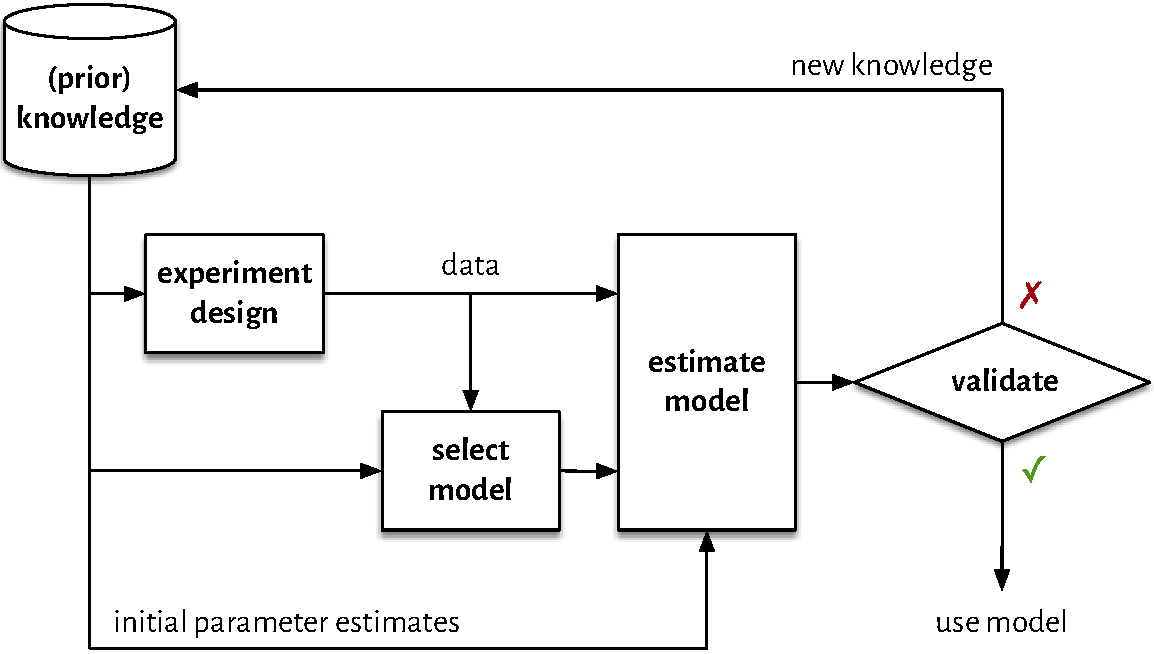
\includegraphics[width=0.9\columnwidth]{\thisDir/figs/id-cycle.pdf}
  \caption[System identification loop]{System identification loop. \disclaimer{Adapted from \citep[Figure 1.10]{Ljung1999} and \citep{Mehra1981}.}}
  \label{fig:intro:identification-cycle}
\end{figure}

\subsection{Linear System theory}
\subsection{System Identification Approaches}

\subsubsection{White Box, Black Box or Grey Box}
\subsubsection{Time or Frequency Domain}
\subsubsection{Linear or nonlinear?}
\subsubsection{Time invariant or non?}

\section{User-friendly System Identification}
In this dissertation, we focus on developing system identification techniques that are `user-friendly'.
User-friendly should be understood as having a good user experience for two groups of users:
\begin{itemize}
  \item novice users, without formal training in system identification, optimization, \ldots and,
  \item well-seasoned identification practitioners that are already able to build good models.
\end{itemize}
Concretely, for novice users it is important to have straightforward techniques that require little interaction.
In practice, this boils down to methods that work well for a wide class of systems.
As such, only very generic assumptions of the system under test should be made and these should be easy to interpret.

For seasoned identification practitioners, methods that require little interaction are an opportunity for automation.
This is especially important for complex systems: systems that have high-order dynamics, \gls{MIMO} systems with a high dimensionality, \ldots
For such complex systems, building a model can be time-consuming and laborious if one has to supervise every step of the process.
For more advanced users, user-friendly methods can hence allow to deal with more complex systems in a shorter amount of time such that the economical cost of building a model is reduced.

In this dissertation, the focus lies on \gls{LTI} systems.
While this might seem as a very restrictive choice, this is one of the fundamental settings for system identification.
In particular, \gls{LTI} systems are a first step to build a system model.
In many cases, such a linear model is accurate enough, e.g. to build a nominal controller, to design electrical filters and obtain a reasonable intuition of the system under test.
Also, most engineers and scientists have a good understanding of linear systems such that \gls{LTI} models align well with their prior knowledge and experience.
Nevertheless, when a linear model is not adequate, a more flexible model needs to be constructed.
Such a model could be more flexible, e.g. by relinquishing the time-invariance and/or its linearity.
However, many of those advanced modeling approaches employ \gls{LTI} models as starting values or intermediate result in building the actual non-linear~\citep{Giri2010} or time-varying model~\citep{Lataire2012,Louarroudi2014}.
As such, improvements in estimating \gls{LTI} models also indirectly improve more advanced methods.

\subsection{Contributions}
In this dissertation, we look into a few aspects of the identification workflow with the goal to make the whole process more user-friendly.

\paragraph{How should a good experiment be designed?}
Can we design a `good experiment' to identify a \gls{LTI} model?
Particularly, this means a robust input signal needs to be constructed without relying on extensive prior knowledge of the system.
Such a signal should cover a wide frequency band to excite all dynamics of the system during the experiment.
However, the signal should ensure that systems in different frequency bands can be identified with a specified level of accuracy.

\paragraph{Can we process the input/output data in a non-parametric way that offers more insight than a standard frequency response function?}


\paragraph{Can we }


\section{Outline and Publications}
   The lion's share of this thesis has been published in either peer-reviewed  journals or conferences.
   This section links my different publications to the different sections in this thesis.
   For an overview of publications grouped by type, please refer to page~\pageref{publicationList}.

\begin{refsection}
% http://tex.stackexchange.com/questions/38580/displaying-selected-bibliographic-items-in-the-body-of-the-text
% http://tex.stackexchange.com/questions/126226/how-do-i-instruct-fullcite-to-use-maxbibnames-rather-than-maxcitenames

\makeatletter
\DeclareCiteCommand{\fullcite}
  {\defcounter{maxnames}{\blx@maxbibnames}%
    \usebibmacro{prenote}}
  {\usedriver
     {\DeclareNameAlias{sortname}{default}}
     {\thefield{entrytype}}}
  {\multicitedelim}
  {\usebibmacro{postnote}}
\DeclareCiteCommand{\footfullcite}[\mkbibfootnote]
  {\defcounter{maxnames}{\blx@maxbibnames}%
    \usebibmacro{prenote}}
  {\usedriver
     {\DeclareNameAlias{sortname}{default}}
     {\thefield{entrytype}}}
  {\multicitedelim}
  {\usebibmacro{postnote}}
\makeatother

% http://tex.stackexchange.com/questions/18664/underline-my-name-in-the-bibliography
% Plus see release notes of BIBLATEX 3.3/3.4
\DeclareNameFormat{author}{%
  \nameparts{#1}%
\ifthenelse{\equal{\namepartfamily}{Geerardyn}}%
    {\textbf{\ifblank{\namepartgiven}{}{\namepartgiven\space}\namepartfamily}}%
    {\ifblank{\namepartgiven}{}{\namepartgiven\space}\ifblank{\namepartprefix}{}{\namepartprefix\space}\namepartfamily}%
\ifthenelse{\value{listcount}<\value{liststop}}%
    {\addcomma\space}
    {}}


The quasi-logarithmic multisines presented in \chapref{sec:excitation} are based on a journal article published in \gls{IEEE} Transactions on Instrumentation \& Measurement:
\begin{itemize}
  \item \fullcite{Geerardyn2013TIM}, 
\end{itemize}
preliminary results were also presented at the 2012 \gls{IFAC} symposium on System Identification (\textsc{SYSID}) and the \gls{IEEE} International Instrumentation and Measurement Conference (\textsc{I$^{\text{2}}$MTC}):
\begin{itemize}
  \item \fullcite{Geerardyn2012IMTC}, and
  \item \fullcite{Larsson2012SYSID}.
\end{itemize}
This work has also been presented at the following local (non-refereed) conferences:
\begin{itemize}
  \item \fullcite{Geerardyn2012Benelux}, and
  \item \fullcite{Geerardyn2012ERNSI}.
\end{itemize}

The non-parametric estimation methods in \chapref{sec:nonparametric} are based on a yet-unpublished manuscript.
 The so-called time-truncated \gls{LPM} that is presented in the same chapter is based on a journal published in \gls{IEEE} Transactions on Instrumentation \& Measurement:
\begin{itemize}
  \item \fullcite{Lumori2014TIM}.
\end{itemize}
In particular, this smoother enables one to reduce the effect of noise on an estimated \gls{FRF} using an automated approach.
Relatedly, a preliminary study of the \gls{LPM} in the context of lightly-damped \gls{MIMO} systems has been presented at the (non-refereed) Benelux Meeting on Systems and Control:
\begin{itemize}
    \item \fullcite{Verbeke2015Benelux}.
\end{itemize}

The use of the non-parametric \gls{FRF} estimation methods for \Hinf gain estimation (and in general the \gls{FRF} interpolation from \chapref{sec:hinf}) has been presented at the 2014 \gls{IFAC} World Conference in South Africa and the 2014 Leuven Conference on Noise and Vibration Engineering (ISMA) in Leuven:
\begin{itemize}
  \item \fullcite{Geerardyn2014IFAC},
  \item \fullcite{Geerardyn2014ISMA}.
\end{itemize}
Preliminary results have been presented at local (non-refereed) conferences:
\begin{itemize}
  \item \fullcite{Geerardyn2013Benelux},
  \item \fullcite{Geerardyn2013ERNSI},
  \item \fullcite{Geerardyn2014Benelux},
  \item \fullcite{Geerardyn2014DYSCO}, and
  \item \fullcite{Geerardyn2014ERNSI}.
\end{itemize}
Experimental work related to \chapref{sec:hinf} has also been presented at the 2015 \gls{IFAC} Symposium on System Identification (\textsc{sysid}) and :
\begin{itemize}
  \item \fullcite{Voorhoeve2015SYSID}
  \item \fullcite{Voorhoeve2015ERNSI}
\end{itemize}

The study of different initialization strategies as depicted in \chapref{sec:initvals} has been published in the \gls{IEEE} Transactions on Instrumentation \& Measurement:
\begin{itemize}
  \item \fullcite{Geerardyn2015TIM},
\end{itemize}
and also at the local (non-refereed) 2015 Benelux Meeting on Systems and Control:
\begin{itemize}
    \item \fullcite{Geerardyn2015Benelux}.
\end{itemize}

In collaboration with fellow researchers, I have written a few other publications.
However, these publications are not covered in this dissertation.

\begin{itemize}
  \item \fullcite{vanBerkel2014Automatica},
  \item \fullcite{Cooman2012SMACD},
  \item \fullcite{Cooman2012DYSCO},
  \item \fullcite{Cooman2012ERNSI}.
\end{itemize}
\end{refsection}



   \chapter{Design of excitation signals}
\label{sec:excitation}
\def\thisDir{ch02-qlogms}
\myEpigraph{A common mistake that people make when trying to design something completely foolproof is to underestimate the ingenuity of complete fools.}{Douglas Adams}{Mostly Harmless}
\researchBasedOn{Larsson2012SYSID, Geerardyn2012IMTC, Geerardyn2013TIM, }

\section{Introduction}
\label{sec:excitation:intro}
Input design deals with the task of choosing an excitation signal in a way so that the information obtained from the experiment is maximized. 
This is a problem which has a long history in statistics. 
In system identification, the focus has mostly been on input design for dynamic systems.
A common approach is to design the input spectrum and thereby maximizing the information matrix of the estimates, see e.g. \citep{Fedorov1972,Goodwin1977}.

A complicating issue in identification of dynamic system is the fact that the information matrix often depends on the true parameter values. 
Consequently, an optimal input design, based on the information matrix, will depend on quantities that are not know at the time of the design.
There are two main solutions to this in the engineering literature~\citep{Goodwin2006GBO}:
\begin{enumerate}
\item Iterative input design where the design updated as more information about the system is available, see e.g.~\citep{Hjalmarsson2005,Gevers2005}.
The disadvantage of this approach is that multiple experiments are required to converge to the optimal design.
Moreover, since the signal is optimized for a specific system model, it is likely that changes in the dynamics are hard to observe using such a signal.

\item Robust (optimal) input design makes the input design robust to uncertainty in the prior knowledge of the parameter values, see e.g.~\citep{Rojas2007,Goodwin2006GBO,Rojas2012} and references therein. 
While the signal is more robust towards uncertainty in the prior knowledge, it requires more forethought than (nominal) optimal designs.
E.g. the approach followed by~\citet{Rojas2007} relies on both nominal parameter values and  knowledge of the distribution function of these parameters to design a robust (optimal) excitation signal.
As such, this requires more advanced prior knowledge of the system to cope with the uncertainty of the prior knowledge.
\end{enumerate}

\subsection{General purpose robust excitation signals}
\label{sec:excitation:intro:approach}
In this chapter, the goal is to construct excitation signals that bridge the properties of general purpose and robust excitation signals to alleviate the chicken-and-the-egg problem that optimal strategies typically incur.
In particular, a generic excitation signal will be used, but its properties are tuned in such a way that it attains some properties of robust excitation signals without requiring extensive prior information.
We will consider input design when it is known that the system has resonances, possibly spanning a frequency band that may cover several decades. 
It is however not necessary to know how many resonances are in the system and at what precise frequencies those may occur.

Such problem settings occur in many diverse fields of experimentation, such as the measurement of biochemical impedances~\citep{Bragos2001,Sanchez2011}, electrochemical impedance spectroscopy~\citep{Niedostatkiewicz2009,VanGheem2004,Breugelmans2010}, electronics~\citep{Munir2011}, mechatronics~\citep{Steinbuch1998,Oomen2016}, vibration analysis~\citep{Karnopp1995,Voorhoeve2015SYSID} and acoustics testing amongst others. %TODO reference acoustics (ISMA?)

  Any \gls{LTI} system of finite order can be expanded into a finite sum of sub-systems of first and second order by means of a partial fraction expansion~\citep{Oppenheim1983}.
  Therefore the performance of the proposed method is assessed on a prototype system of second order.
  This does not limit the generality of the approach as we can add several of such systems to construct a general \gls{LTI} system.
  
  To ensure that any second order system with its resonance frequency in the specified frequency range is measured with an equal accuracy, the system output should contain a comparable power level irrespective of its resonance frequency.
  For a system with a sufficiently low damping, one can intuitively understand that most of the information is contained within the $3 \unit{dB}$ bandwidth of the system.
  Remember that an \gls{LTI} system is naturally described in a logarithmic frequency axis (the slopes of such a system are specified in $\unit{dB}/\text{decade}$).
  Hence, an excitation with a flat power spectrum and a linearly spaced frequency grid will over-excite the high end of the band at the cost of the low frequencies.
  To restore equal excitation signal levels over the complete range of frequencies, we will need to distribute the power in $1/\omega$ over the frequency band~\citep{Goodwin2006,Goodwin2006GBO}.
  In a noise excitation context, this results in pink noise.
  In a periodic setting, this results in a multisine whose frequency components are spaced equidistantly on a logarithmic axis.
  
  The main problem is that network and dynamic signal analyzers typically
  rely on an equidistant frequency grid that comes with the \gls{DFT}.
  A logarithmically spaced signal, on the other hand, does not match well to an equidistant frequency grid.
  More specifically, the lack of frequency resolution at the lowest frequencies hampers the quality of the power distribution at the low edge of the frequency band.
  To circumvent this disadvantage, we will construct quasi-logarithmically spaced signals.
  Their frequency spacing is approximately logarithmic but nevertheless conforms to the linear frequency grid of the \gls{DFT}.

  We will also present a simple method to determine a suitable density of a logarithmically spaced signal for a predefined minimal damping of the system to be tested.

  \paragraph{Contents}
  In \secref{sec:excitation:inputDesign}, we first consider (optimal) input design for an example second-order system.
  \secref{sec:excitation:logarithmic} expounds the use of a signal with $1/f$  power spectrum on some basic sub-systems.
  Next, in \secref{sec:excitation:parametrization} \gls{LTI} systems are parametrized to facilitate a robust input design based on the observations of the preceding section.
  In \secref{sec:excitation:multisine} a comparison of different discrete frequency grids is provided, this is related to the problem of generating a multisine signal with a $1/f$ power spectral density.
  Next, \secref{sec:excitation:optimAlpha} describes the selection of a suitable frequency ratio $\alpha$ for a logarithmically spaced grid such that constant model quality is obtained.
  The usefulness of the proposed signals is illustrated on simulations in \secref{sec:excitation:simulation} and validated on the measurement of a set of band-pass filters in \secref{sec:excitation:measurement}.
  Conclusions are formulated in \secref{sec:excitation:conclusion}.

\section{Input design}
\label{sec:excitation:inputDesign}
For the theoretical analysis, we consider \gls{SISO} \gls{OE} systems, i.e.
\begin{align}
y(t) &=G(s,\theta)u(t)  + e(t),
\end{align}
where $u(t)$ is a known input sequence, $y(t)$ the output sequence, and $e(t)$ is zero mean Gaussian white noise with variance $\sigma_{e}^2$.
$G$ is a rational, time invariant transfer function in continuous time.
For notational simplicity, $s$ is used both as the complex Laplace variable and the differentiation operator; it should be clear from the context which is used. 
The transfer function is parameterized by the vector $\theta$.
These parameters are unknown and hence we are interested in estimating their values. 

The goal of input design is to find an input that under the given experimental conditions, gives as much information as possible about the system.
This can be done by optimizing the input power spectrum such that  a scalar criterion involving the Fisher information matrix is minimized.

In open loop experiments, the scaled average information matrix is given by
\begin{align}
\IF & = \lim_{N\rightarrow\infty}
          \frac{1}{N}
            \sum_{t=1}^{N}
              {\left(\frac{\partial\hat{y}(t)}{\partial\theta}\right)
               \left(\frac{\partial\hat{y}(t)}{\partial\theta}\right)^{\T}},\\
\frac{\partial\hat{y}(t)}{\partial\theta}
    & =\frac{\partial G(s,\theta)}{\partial \theta}u(t).
\end{align}
By Parseval's theorem, $\IF$ can be expressed as
\begin{align}
\IF &= \frac{1}{\pi}
         \int\limits_0^\infty \mathrm{Re}
           \left\{      \frac{\partial G(j\omega)}{\partial \theta}
                  \left[\frac{\partial G(j\omega)}{\partial \theta}\right]^{\HT}
           \right\}
           \powerspec{u}(j\omega)
           \dd{\omega} \text{.}
\label{eq:excitation:IF}
\end{align}
The information matrix is a function of the input power spectrum $\powerspec{u}$, which is the only entity that can be used to improve the quality of the estimates. 
A common optimality criterion is D-optimality where $\det{\IF}$ is maximized~\citep{Goodwin1977}.

\begin{remark}
D-optimal input designs are quite popular since this criterion minimizes the volume of uncertainty ellipsoid of the parameters.
Moreover, the D-optimal input design is independent of the parametrization of the system (as long as the different parametrizations can be related by a bijective function)~\citep[Chapter 6]{Goodwin1977}.
\end{remark}

The information matrix tells us how good the individual parameter estimates are. However, if we are interested in estimating a transfer function $G(s,\theta)$ the quality of this estimate is of more importance. 
It is possible to find an expression for the variance of $\hat{G}(j\omega,\theta)$ using the Gauss approximation formula \citep{Ljung1999, Pintelon2012}. This gives
\begin{align}
\var{\hat{G}(j\omega)} &\approx \frac{\partial G^H(j\omega)}{\partial \theta}\IF^{-1}\frac{\partial G(j\omega)}{\partial \theta}.
\label{eq:excitation:varG}
\end{align}

Typically, the input design formulation depends on the true system parameters. This means that the optimal input depends on the \emph{unknown} system that one wants to identify. 
Furthermore, classical input designs, such as the D-optimal design, typically give signals with sparse spectra. 
This means that only a few frequencies are excited. 
A sparse spectrum is bad from a robustness point of view; there is very limited information about what happens at the unexcited frequencies. 
Therefore, a signal design to be optimal for one system may result in very bad estimates if applied to another system.
To increase the robustness of the design, one could take a small fraction $\delta$, from the optimal power and redistribute this power over the whole frequency band of interest.
From \eqref{eq:excitation:IF} and \eqref{eq:excitation:varG} we see that scaling the input power by $1-\delta$, gives the transfer function variance
\begin{align}
\var{\hat{G}(j\omega)}\frac{1}{1-\delta}.
\end{align}
This is a small loss while the increase in robustness can be significant if the added signal is robust. Such a robust signal is studied in the following parts of the chapter.

\section{Logarithmic power distributions}
\label{sec:excitation:logarithmic}
When no information about the system is known, it is desirable that the excitation signal is such that regardless of the true system characteristics, the resulting estimates have equally good statistical properties.
This can be ensured by a suitable choice of the input power spectrum.

 \subsection{A second order system}
Consider the second order system
\begin{align}
y(t) 
  &= 
  G(s,\theta) u(t) 
  = \frac{1}
                {\frac{s^2}{\wn^2} + 2\frac{\damping}{\wn}s + 1}
      u(t),
\label{eq:excitation:2ndOrderSys}
\end{align}
with parameters $\theta=[\wn\;\damping]^{\T}$. 
The resonance frequency of the system is $\wR \isdef \sqrt{1-\damping^2}\wn$.
  
When $\damping < \frac{1}{\sqrt{2}}$, such a second order system exhibits a peak in the amplitude of the transfer function~\citep{Oppenheim1983}:
  \begin{align}
   \left| G\left(\wM \right) \right| & \isdef
          \max_{\omega} \left| G\left( \omega \right)  \right|
        = \frac{1}
               {2 \damping \sqrt{1-\damping^2}}
               \label{eq:excitation:peakAmplitude}\\
   \wM &
        = \sqrt{1-2\damping^2} \wn
        \label{eq:excitation:peakFrequency}
    \text{.}
  \end{align}
  The $3\unit{dB}$ bandwidth around this resonance peak is given by $\wdB = 2\damping\wn$ for systems that have a sufficiently low damping.

Since information is local in the frequency domain, the input signal power inside $\wdB$, contributes significantly to the information matrix while input power outside $\wdB$ has a smaller contribution. This can be seen by considering the optimal design for a second order system. From \citep[Example 6.4.5]{Goodwin1977} we have that the D-optimal design for \eqref{eq:excitation:2ndOrderSys} is a single sinusoid at frequency
\begin{align}
\omega^\star =\frac%
{\wn
  \sqrt{
    \left(1-2\damping^2\right)
    +
    \sqrt{\left(1-2\damping^2\right)^2+15}
    }
  }
{\sqrt{5}}.
\label{eq:excitation:optFreq}
\end{align}
For lightly-damped systems, i.e $\damping \ll 1$ , $\omega^\star\approx \wn$, which is inside the bandwidth of the system. 
From \eqref{eq:excitation:optFreq} it is clear that the optimal design depends on the resonance of the system to be identified. 
Input design can be based on a guess of $\wn$, however if this guess is wrong, the resulting estimates may be unacceptable~\citep{Rojas2007}.

When no information about the system is available, we propose using an input power spectrum with a logarithmic power distribution. This can be achieved either with a continuous band-limited $1/f$ spectrum or a quasi-logarithmic multisine spectrum \citep{Pintelon2012}. 
We choose to work with an equidistant frequency grid with resolution $f_0$ and design the input in the frequency band $[\wn \kMin\; \wn \kMax]$, where the resolution is $k_0=1/\Tm$ and $\Tm$ is the measurement time. 
Hence, a finite measurement time limits the frequency resolution and therefore we have to put a lower limit on the frequency band of interest. Moreover, we can only impose the logarithmic distribution sufficiently well if $\kMin$ is large enough.

First, we look at the band-limited $1/f$ power spectrum given by
\begin{align*}
\label{eq:excitation:pink}
\phi_u(\omega) &=\begin{cases}\frac{1}{|\omega|} &\text{if $|\omega|\in[\wn \kMin\; \wn \kMax]$,}\\
                        0           &\text{otherwise}.
            \end{cases}
\end{align*}
With this input spectrum, the power inside $\wdB$ is
\begin{align}
  \frac{1}{2\pi}
    \int\limits_{(1-\damping)\wn}^{(1+\damping)\wn}
     \frac{1}{\omega} \dd{\omega}
  = \frac{1}{2\pi}
    \ln{\frac{1+\damping}{1-\damping}},
\end{align}
which is independent of $\wn$. The robustness of the $1/f$ input has been noted previously by e.g. \cite{Rojas2007}

Alternatively, one could also construct a signal with power spectrum concentrated at discrete frequency lines.
Such signals are elaborated in \secref{sec:excitation:multisine}.

% Second, we consider the power spectrum of the quasi-logarithmic multisine signal [\cite{Pintelon2012}] given by
% \begin{align}
%   \phi_u(\omega) &= \frac{1}{M}\sum_{k=1}^{M}{\dirac{\omega - \omega_k}},
% \end{align}
% where $\omega_{k}/\omega_{k+1} \approx \alpha$ and $\dirac{\omega}$ denotes the Dirac distribution.
% Hence, the number of spectral lines inside \wdB is 
% \begin{align}
%   \floor{
%     \log_{\alpha} \frac{1+\damping}{1-\damping} 
%   }
%   \text{,}
% \end{align}
% where $\floor{\placeholder}$ is the nearest integer rounded downwards. 
% The number of spectral lines is independent of $\wn$. 

% More generally, a multisine can be defined as:
% \begin{equation}
%  u \left[ n\right] = \frac{1}{\sqrt{F}}
%    \sum_{k=1}^{F} 
%      A_k 
%      \sin 
%        \left(\frac{2\pi n k f_0}{f_s} + \psi_k \right)
%   \label{eq:excitation:MS}
% \end{equation}
% where $A_k$ and $\psi_k$ are its amplitude and phase spectrum; $f_s$ is the
% sampling frequency and $f_0 = \frac{f_s}{N}$ the base frequency with $N$ the 
% number of points in a period. 

% To construct a quasi-logarithmic multisine, only frequency lines $f_j$ within the set of available sine components $\left\{f_0, 2 f_0, \ldots, F f_0  \right\}$ are excited for which the ratio of two consecutive frequencies $f_j$ and $f_{j-1}$ is approximately constant: $\frac{f_{j-1}}{f_j} \approx \alpha$.

The result of these two choices of input power spectrum is that for a given damping, $\var{\hat{G}}$ is approximately the same independent of $\wn$. 
This is illustrated in \secref{sec:excitation:simulation}.

\subsection{Sums of second order systems}
This section extends the previous section to more general systems than second order.
Consider a system
\begin{align}
G(s,\theta) &= \sum_{i=1}^{K} G_i(s,\theta_i)
             =\sum_{i=1}^{K}  \frac{1}
                                   {   \frac{s^2}{\wn[i]^2}
                                    + 2\frac{\damping[i]}{\wn[i]}s
                                    + 1},\\
\theta_i&=[\wn[i]\;\damping[i]]^{\T}.
\label{eq:excitation:sumSys}
\end{align}
The systems  $G_i$ will be called the \emph{sub-systems} of $G$. 
Without loss of generality, we assume that $\wn[1] < \wn[2] < \cdots < \wn[K]$. 
To properly identify the system $G$, excitation is required such that all subsystems are properly excited, regardless of their individual resonance frequencies.

The information matrix for systems of the type \eqref{eq:excitation:sumSys} will have a block structure commensurate with the dimension of $\theta_i$ given by
\begin{align}
\IF &= \frac{1}{\pi}
\begin{bmatrix}
  \partial G_{1,1}        &\partial G_{1,2}       &\deemph{\cdots}         &\partial G_{1,K}\\
  \partial G_{2,1}        &\partial G_{2,2}       &\deemph{\cdots}         &\partial G_{2,K}\\
  \deemph{\vdots}                  &\deemph{\vdots}                 &\deemph{\ddots}         &\deemph{\vdots}          \\
  \partial G_{K,1}        &\partial G_{K,2}       &\deemph{\cdots}         &\partial G_{K,K}
\end{bmatrix},\\
\partial G_{i,j} &= \int_0^\infty
                      \mathrm{Re}\left\{
                          \frac{\partial G_i}
                               {\partial \theta_i}
                          \frac{\partial G_j^{\HT}}
                               {\partial \theta_j}
                                \right\}
                      \phi_u(\omega)\dd\omega.
\end{align}

Furthermore, when the damping of the systems is low or the resonances of the sub-systems are well separated, the estimates decouple in the sense that the elements off-diagonal blocks become small.
The effect is that the variance of the estimated transfer function approximately becomes the sum of the variances of the sub-systems.
To illustrate this we look at a system with $K=2$, i.e. the sum of two second order systems.
The conclusions from the example are easily extended to systems consisting of more than two sub-systems.

\subsubsection{Example: Sum of two second-order systems}
\label{sec:excitation:ex:sumOfSecondOrderSipmle}
Consider the system
\begin{align}
G(s,\theta) &= G_1(s,\theta_1) + G_2(s,\theta_2)%\\
%&=\frac{1}{\frac{s^2}{\wn[1]^2} + 2\frac{\damping[1]}{\wn[1]}s + 1} + \frac{1}{\frac{s^2}{\wn[2]^2} + 2\frac{\\damping[2]}{\wn[2]}s + 1},
\end{align}
with $\theta_1=[\wn[1]\;\damping[1]]^{\T}$ and $\theta_2=[\wn[2]\;\damping[2]]^{\T}$.
The information matrix for this system is
\begin{align}
\IF &=
       \begin{bmatrix}
         \partial G_{1,1}  & \partial G_{1,2}\\
         \partial G_{2,1}  & \partial G_{2,2}
       \end{bmatrix}.
\label{eq:excitation:infoEx}
\end{align}
To investigate the decoupling, we study the $(1,1)$ elements of blocks $\partial G_{1,1}$ and $\partial G_{1,2}$ of the information matrix \eqref{eq:excitation:infoEx}, when the input spectrum \eqref{eq:excitation:pink} is used; similar arguments can be made for the other elements of the two matrix blocks.

Direct calculations for $\damping < 1$ give
\begin{align}
\label{eq:excitation:auto}
\int_0^\infty\mathrm{Re}\left\{\frac{\partial G_1}{\partial \wn[1]}\frac{\partial G_1^{\HT}}{\partial \wn[1]}\right\}\frac{1}{\omega}\dd\omega = \frac{\pi}{16\wn[1]^2}\damping^{-3} + \mathcal{O}(\damping^{-1}).
\end{align}
For the corresponding element in $\partial G_{1,2}$ we start by bounding the absolute value of the integral by
\begin{gather}
\left|\int_0^\infty\mathrm{Re}\left\{\frac{\partial G_1}{\partial \wn[1]}\frac{\partial G_2^{\HT}}{\partial \wn[2]}\right\}\frac{1}{\omega}\dd\omega\right|
\qquad \qquad \qquad \qquad \qquad
\label{eq:excitation:cross1} \\
\leq
\int_0^\infty\left|\mathrm{Re}\left\{\frac{\partial G_1}{\partial \wn[1]}\frac{\partial G_2^{\HT}}{\partial \wn[2]}\right\}\right|\frac{1}{\omega}\dd\omega
\leq \\
\qquad \qquad \qquad \qquad \qquad
\int_0^\infty\left|\frac{\partial G_1}{\partial \wn[1]}\frac{\partial G_2^{\HT}}{\partial \wn[2]}\right|\frac{1}{\omega}\dd\omega \text{.}\label{eq:excitation:cross}
\end{gather}
To proceed, consider
\begin{align}
\frac{\partial G_1}{\partial \wn[1]} 
  &= \frac{2\damping j\omega\left[1+\frac{j\omega}{\wn[1]\damping}\right]}
  {\wn[1]^2\left[1+2\frac{\damping j\omega}{\wn[1]} + \left(\frac{j\omega}{\wn[1]}\right)^2\right]^2},
\end{align}
which has zeros in $j\omega=\left\{0, \damping\wn[1]\right\}$. 
Hence $\left|\frac{\partial G_1}{\partial \wn[1]} \right|$ has asymptotic slope 20\unit{dB/\decade} for low frequencies, at $j\omega=\damping\wn[1]$ the slope increases to 40\unit{dB/\decade}. 
There are four poles which give a $-40$\unit{dB/\decade} roll-off after the peak. 
The shape of $\frac{\partial G_1}{\partial \wn[1]} $ is illustrated in \figref{fig:excitation:derivatives}.

A crude, albeit useful, bound on the integrand in \eqref{eq:excitation:cross} is
\begin{align}
&f\left(\omega,\theta_1,\theta_2\right)=
  \begin{cases}
   \frac{\omega^2}{\wn[1]^2}
   \frac{1}{\omega}
   \partial G_1^\infty
                                       & \text{if $\omega \leq \wn[1]$,}\\
   \phantom{\frac{\omega^2}{\omega^2}}
   \frac{1}{\omega}
   \partial G_1^\infty
                                       & \text{if $\wn[1] < \omega < \wn[2]$,}\\
   \frac{\wn[2]^2}{\omega^2}
   \frac{1}{\omega}
   \partial G_1^\infty
                                       & \text{if $\omega \geq \wn[2]$,}
  \end{cases}
\end{align}
where $\partial G_1^\infty = \left\|\frac{\partial G_1}{\partial \wn[1]}\right\|_\infty$. 
Again, direct calculations give
\begin{align}
\int_0^\infty f\left(\omega,\theta_1,\theta_2\right)\dd\omega = \frac{\wn[1]\left(2-\ln{\frac{\wn[1]^2}{\wn[2]^2}}\right)}{\wn[2]^2}\damping^{-2} + \mathcal{O}(1).
\end{align}
Hence \eqref{eq:excitation:cross1} cannot grow faster than $\mathcal{O}(\damping^{-2})$ as $\damping\rightarrow0$. From this analysis we conclude that:
\begin{itemize}
\item the integral \eqref{eq:excitation:cross1} decreases as $\wn[2]-\wn[1]$ increases, and
\item lower damping further decreases the integral \eqref{eq:excitation:cross1} in comparison to \eqref{eq:excitation:auto}.
\end{itemize}

To further illustrate the decoupling of the two systems, we calculate \eqref{eq:excitation:infoEx} for different values of the damping $\damping$ and separations of the two resonances $\wn[1]$ and $\wn[2]$. If the separation is taken in terms of $\wdB$-units for the lower resonance, the result only depends on the difference $\wn[1]-\wn[2]$ and not on the actual frequencies. The resulting information matrix is then normalized so that the largest element is $1$.

In \figref{fig:excitation:coupling} the largest element in $\partial G_{1,2}$ is plotted for different dampings and separations. It is clear that highly resonant systems have a large degree of decoupling and that resonances that are well-separated increases the decoupling. 
The diagonal blocks of the normalized $\IF$ in all cases have some elements close to $1$. 
In this example, the $\damping$ is set to be the same in both sub-systems. 
Using different dampings in the sub-systems would, however, not change the argument, the systems with the lowest damping will limit the separation.

Based on the above arguments, we approximate the information matrix for lightly-damped systems as a block-diagonal matrix:
\begin{align}
\IF&\approx \begin{bmatrix}\partial G_{1,1} &\deemph{0}\\
                        \deemph{0}&\partial G_{2,2}\end{bmatrix}.
\end{align}
Hence the variance of the estimate $\hat{G}(s,\theta)$ becomes
\begin{align}
\var{\hat{G}(\omega)} &\approx \frac{\partial G^{\HT}(e^{j\omega})}{\partial \theta}\begin{bmatrix}\partial G_{1,1} &\deemph{0}\\
                        \deemph{0}&\partial G_{2,2}\end{bmatrix}^{-1}\frac{\partial G(e^{j\omega})}{\partial \theta}\\
&=\var{\hat{G}_1(\omega)} + \var{\hat{G}_2(\omega)}.
\end{align}

This results extends mutatis mutandis to systems consisting of more sub-systems.

\begin{figure}
\centering
\setlength\figurewidth{0.68\columnwidth}
\setlength\figureheight{0.68\figurewidth}
% This file was created by matlab2tikz v0.1.1.
% Copyright (c) 2008--2011, Nico Schlömer <nico.schloemer@gmail.com>
% All rights reserved.
% 
% The latest updates can be retrieved from
%   http://www.mathworks.com/matlabcentral/fileexchange/22022-matlab2tikz
% where you can also make suggestions and rate matlab2tikz.
% 
\begin{tikzpicture}
\begin{axis}[%
scale only axis,
width=\figurewidth,
height=\figureheight,
ymode=log,
xmin=1e-005, xmax=0.7,
ymin=1e-007, ymax=1,
xlabel={Damping $\damping$},
ylabel={Largest normalized coupling element of $\IF$},
%xtick={0.1,0.2,0.3,0.4,0.5,0.6,0.7},
ytick={1e-7,1e-5,1e-3,1e-1},grid=major,
legend pos=south east,
cycle list name=linestyles*]

\addplot table[row sep=crcr]{
1e-005	0.00956784\\
1.46917e-005	0.00956848\\
2.15846e-005	0.00956943\\
3.17115e-005	0.00957083\\
4.65896e-005	0.00957288\\
6.84482e-005	0.0095759\\
0.000100562	0.00958033\\
0.000147743	0.00958684\\
0.000217059	0.00959641\\
0.000318898	0.00961047\\
0.000468515	0.00963114\\
0.000688329	0.00966153\\
0.00101127	0.00970623\\
0.00148573	0.009772\\
0.00218279	0.00986886\\
0.0032069	0.0100117\\
0.00471148	0.0102225\\
0.00692197	0.0105346\\
0.0101696	0.0109981\\
0.0149408	0.01169\\
0.0219506	0.0127302\\
0.0322492	0.0143103\\
0.0473796	0.0167451\\
0.0696088	0.0205684\\
0.102267	0.026706\\
0.150248	0.0367524\\
0.22074	0.0532791\\
0.324305	0.0798266\\
0.476459	0.120062\\
0.7	0.175033\\
};
\addlegendentry{$\wn[2] - \wn[1] = 4\wdB$};

\addplot table[row sep=crcr]{ 
1e-005	0.000695711\\
1.46917e-005	0.000695812\\
2.15846e-005	0.000695962\\
3.17115e-005	0.000696182\\
4.65896e-005	0.000696504\\
6.84482e-005	0.000696979\\
0.000100562	0.000697676\\
0.000147743	0.0006987\\
0.000217059	0.000700207\\
0.000318898	0.000702422\\
0.000468515	0.000705682\\
0.000688329	0.000710482\\
0.00101127	0.000717556\\
0.00148573	0.000728001\\
0.00218279	0.000743457\\
0.0032069	0.000766407\\
0.00471148	0.000800661\\
0.00692197	0.000852188\\
0.0101696	0.000930613\\
0.0149408	0.00105211\\
0.0219506	0.00124533\\
0.0322492	0.00156422\\
0.0473796	0.00211629\\
0.0696088	0.00312326\\
0.102267	0.00504068\\
0.150248	0.00875851\\
0.22074	0.0158595\\
0.324305	0.0288538\\
0.476459	0.0517209\\
0.7	0.095736\\
};
\addlegendentry{$\wn[2] - \wn[1] = 8\wdB$};

\addplot table[row sep=crcr]{
 1e-005	4.52139e-005\\
1.46917e-005	4.52274e-005\\
2.15846e-005	4.52472e-005\\
3.17115e-005	4.52763e-005\\
4.65896e-005	4.53191e-005\\
6.84482e-005	4.5382e-005\\
0.000100562	4.54745e-005\\
0.000147743	4.56105e-005\\
0.000217059	4.58106e-005\\
0.000318898	4.61052e-005\\
0.000468515	4.65396e-005\\
0.000688329	4.7181e-005\\
0.00101127	4.81303e-005\\
0.00148573	4.9541e-005\\
0.00218279	5.16494e-005\\
0.0032069	5.48301e-005\\
0.00471148	5.96997e-005\\
0.00692197	6.73309e-005\\
0.0101696	7.9732e-005\\
0.0149408	0.00010098\\
0.0219506	0.000139973\\
0.0322492	0.000217012\\
0.0473796	0.000378608\\
0.0696088	0.000727808\\
0.102267	0.0014789\\
0.150248	0.00304147\\
0.22074	0.00612406\\
0.324305	0.011842\\
0.476459	0.022061\\
0.7	0.0430551\\
};
\addlegendentry{$\wn[2] - \wn[1] = 16\wdB$};

\addplot table[row sep=crcr]{
 1e-005	2.85537e-006\\
1.46917e-005	2.85708e-006\\
2.15846e-005	2.8596e-006\\
3.17115e-005	2.8633e-006\\
4.65896e-005	2.86873e-006\\
6.84482e-005	2.87672e-006\\
0.000100562	2.88848e-006\\
0.000147743	2.90579e-006\\
0.000217059	2.9313e-006\\
0.000318898	2.96898e-006\\
0.000468515	3.02475e-006\\
0.000688329	3.10766e-006\\
0.00101127	3.23176e-006\\
0.00148573	3.41963e-006\\
0.00218279	3.70946e-006\\
0.0032069	4.17095e-006\\
0.00471148	4.94374e-006\\
0.00692197	6.33587e-006\\
0.0101696	9.08064e-006\\
0.0149408	1.49915e-005\\
0.0219506	2.85425e-005\\
0.0322492	6.039e-005\\
0.0473796	0.000134549\\
0.0696088	0.000301814\\
0.102267	0.000662761\\
0.150248	0.00140266\\
0.22074	0.00283444\\
0.324305	0.0054419\\
0.476459	0.0100217\\
0.7	0.019292\\
};
\addlegendentry{$\wn[2] - \wn[1] = 32\wdB$};

\addplot
table[row sep=crcr]{%
 1e-005	1.79126e-007\\
1.46917e-005	1.79341e-007\\
2.15846e-005	1.79657e-007\\
3.17115e-005	1.80121e-007\\
4.65896e-005	1.80804e-007\\
6.84482e-005	1.8181e-007\\
0.000100562	1.83293e-007\\
0.000147743	1.85482e-007\\
0.000217059	1.88724e-007\\
0.000318898	1.93549e-007\\
0.000468515	2.00792e-007\\
0.000688329	2.11825e-007\\
0.00101127	2.29077e-007\\
0.00148573	2.57283e-007\\
0.00218279	3.06753e-007\\
0.0032069	4.02308e-007\\
0.00471148	6.07766e-007\\
0.00692197	1.09122e-006\\
0.0101696	2.28942e-006\\
0.0149408	5.29174e-006\\
0.0219506	1.26689e-005\\
0.0322492	3.01521e-005\\
0.0473796	6.98889e-005\\
0.0696088	0.00015651\\
0.102267	0.000337685\\
0.150248	0.000700247\\
0.22074	0.00138966\\
0.324305	0.00262784\\
0.476459	0.00477076\\
0.7	0.00900354\\
};
\addlegendentry{$\wn[2] - \wn[1] = 64\wdB$};

\draw [->, line width=1pt]
(axis cs:0.4,0.3) -- (axis cs:0.52,0.0006);

\end{axis}
\end{tikzpicture}

\caption[Relative amplitudes of the off-diagonal blocks of the Fisher information matrix.]{The element with the largest absolute value in the off-diagonal blocks of the normalized information matrix for different dampings.
         The different plots are for different separations of the resonance frequencies, from 4\wdB to 64\wdB.
         The arrow indicates the direction of increasing separation.}
\label{fig:excitation:coupling}
\end{figure}

\section{System parametrization} 
\label{sec:excitation:parametrization}

  We consider the transfer function models of proper \gls{LTI} systems of arbitrary but finite orders $\order{B} / \order{A}$:
  \begin{align}
    G\left( \Omega, \theta \right) 
    = \frac{B\left( \Omega,\theta \right)}
                  {A\left( \Omega,\theta \right)}
    = \frac{\sum\limits_{i=0}^{\order{B}} b_i \Omega^i}
                  {\sum\limits_{i=0}^{\order{A}} a_i \Omega^i}
    \text{.} 
    \label{eq:excitation:model}
  \end{align}
  
The model is parametrized by the vector $\theta = \left[b_0 \,\cdots\, b_{n_b-1} \; a_0 \,\cdots\, a_{n_a-1} \right]^{\T}$ and  is evaluated at different frequencies $\Omega$ in the complex plane.
For a continuous time model $\Omega = s$, while for the discrete time case $\Omega = z$.
For the sake of notational simplicity, $\Omega = s$ will be used further on, but the results are similar for $\Omega=z$.
Remember that the rational transfer function of any strictly proper \gls{LTI} system $G$ can be decomposed in its partial fraction form~\citep[Appendix]{Oppenheim1996}:
\begin{align}
  G(s) &= 
    \frac{\sum\limits_{i=0}^{\numel{B}} b_i s^i}
              {\sum\limits_{i=0}^{\numel{A}} a_i s^i} 
        =    
   \frac{\sum\limits_{i=0}^{\numel{B}} b_i s^i}
              {\prod\limits_{i=1}^{I_1} \left( s - \pole[i] \right)^{M_{1,i}} 
               \prod\limits_{i=1}^{I_2} \left(s^2 + 2 \damping[i] \wn[i] s + \wn[i]^2 \right)^{M_{2,i}}}
        \\
        &  = 
        \sum_{i=1}^{I_1} 
          \sum_{\multiplicity=1}^{M_{1,i}} 
            \frac{\dc[i]}
                      { \left( s - \pole[i] \right)^{\multiplicity}}
            + 
        \sum_{i=1}^{I_2} 
          \sum_{\multiplicity=1}^{M_{2,i}}
           \frac{\dc[i,\multiplicity] \wn[i]^{2\multiplicity} \left( s + \wz[i] \right)}
                     {\wz[i] \left(s^2 + 2 \damping[i] \wn[i] s + \wn[i]^2 \right)^{\multiplicity}}
        \label{eq:excitation:PFE}
\end{align}
where $I_1$ denotes the number of real-valued poles, $I_2$ denotes the number of complex conjugated pole pairs.
$M_{1,i}$ and $M_{2,i}$ denotes the multiplicity of the corresponding poles, such that $\numel{A} = \sum_i^{I_1} M_{1,i} + 2 \sum_{i}^{I_2} M_{2,i}$.
Each term in \eqref{eq:excitation:PFE} represents a \term{sub-system} of the system $G(s)$.
  Within these sub-systems, we can distinguish first-order subsystems and second-order subsystems, the latter of which describe resonant phenomena.
  Since such resonances are often a limiting factor, we first focus on these resonant sub-systems.
\begin{remark}
  For non-proper systems, one can write the transfer function $G_{\mathrm{non-proper}}(s) = P(s) + G_{\mathrm{proper}}$ where $P(s)$ is a polynomial and $G_{\mathrm{proper}}(s)$ a proper rational function.
  As such, the polynomial $P(s)$ should be added to equation \eqref{eq:excitation:PFE} for non-proper systems.
\end{remark}

Consider the second-order subsystem with multiplicity $\multiplicity$:
\begin{equation}
  G_2(s, \theta) = \frac{\dc \wn^{2 \multiplicity} \left( s + \wz \right)}{\wz \left(s^2 + 2 \damping \wn s + \wn^2 \right)^{\multiplicity}}
\label{eq:excitation:secondOrderSubsystem}
\end{equation}
parametrized in $\theta =  \left[K, \wn, \wz, \damping \right]^{\T}$.
To determine the Fisher Information matrix, the derivative $\PartialDerivative{G(s,\theta)}{\theta}$ is required; its components are given by:
\begin{align}
  \PartialDerivative{G_2}{\dc} 
    &= 
    \frac{G_2}{\dc}
    =
  \frac{\wn^{2\multiplicity}}{\wz}
  \frac{s + \wz}{\left(s^2 + 2 \damping \wn s + \wn^2\right)^{\multiplicity}}
  \\
  \PartialDerivative{G_2}{\wz} 
    &= 
    \frac{-\dc \wn^{2\multiplicity}}
              {\wz} 
    \frac{s}
              {\left(s^2 + 2 \damping \wn s + \wn^2\right)^{\multiplicity}} 
  \\
  \PartialDerivative{G_2}{\wn} 
  &= 
  \frac{2 \dc \wn^{2\multiplicity-1} \multiplicity}
            {\wz} 
  \frac{\left( s + \wz \right) \left( s+ \damping \wn \right)}
            {\left( s^2 + 2 \damping \wn s + \wn^2 \right)^{\multiplicity + 1}}
  \\
  \PartialDerivative{G_2}{\damping}
  &= 
  \frac{-2 \dc \wn^{2\multiplicity + 1} \multiplicity}
            {\wz}
  \frac{s \left( s + \wz \right)}
             {\left( s^2 + 2 \damping \wn s + \wn^2 \right)^{\multiplicity + 1}}
  \text{.}
\end{align}

The poles of these derivatives coincide with the system poles (possibly with increased multiplicity).
Consequently, this means that for lightly-damped systems ($\damping \ll \sqrt{2}$), these derivatives exhibit a sharp resonance peak at the same frequency as the actual sub-system $G_2$, see also \figref{fig:excitation:derivatives}.
The roll-off near the resonance is determined mainly by the damping $\damping$ and the multiplicity $\multiplicity$ of the sub-system.
The relationship between the frequency of the zero $\wz$ and the resonance frequency $\wn$ alters the shape of these derivatives, but has little impact in the vicinity of the resonance peak.
As such, the Fisher information matrix is pre-dominantly determined by the input power spectrum near $\wn$.
Note that $\PartialDerivative{G_2}{\wn}$ and $\PartialDerivative{G_2}{\damping}$ have the steepest roll-off near the resonance.
As such, those parameters are the most important for the experiment design.

\begin{figure}
  \centering
  \setlength\figurewidth{0.9\columnwidth}
  \setlength\figureheight{\figurewidth}
  \begin{tikzpicture}

\def\varWn{1}
\def\varWzSmall{0.1}
\def\varWzBig{10}
\def\varK{0.5}
\def\varXi{0.025}

% command to compute amplitude of TF (#1+j#2)/(#3+j#4)
\newcommand{\amplitudeTf}[4]{sqrt((#1)^2 + (#2)^2)/sqrt((#3)^2 + (#4)^2)}

% definition of the derivatives for the (K, wn, wz, xi) and \omega = x
\newcommand{\dGdK}[4]{(#2)^2/(#3)*\amplitudeTf{#3}{x}{2*(#4)*(#2)*x}{(#2)^2-x^2}}
\newcommand{\dGdWz}[4]{(#1)*(#2)^2/(#3)*\amplitudeTf{0}{x}{2*(#4)*(#2)*x}{(#2)^2-x^2}}
\newcommand{\dGdWn}[4]{2*(#1)*(#2)/(#3)*\amplitudeTf{(#4)*(#2)*(#3)-x^2}{x*((#3)+(#2)*(#4))}{((#2)^2 - x^2)^2 - 4*(#2)^2*x^2*(#4)^2}{4*(#2)*x*(#4)*((#2)^2 - x^2)}}
\newcommand{\dGdXi}[4]{2*(#1)*(#2)^3/(#3)*\amplitudeTf{-x^2}{(#3)*x}{((#2)^2 - x^2)^2 - 4*(#2)^2*x^2*(#4)^2}{4*(#2)*x*(#4)*((#2)^2 - x^2)}}
% Use MATLAB/mupad to derive the equations in terms of (K, wn, wz, xi)
% Then, retrieve real/imag parts
% Then, replace K -> (#1), wn -> (#2), etc.

\pgfplotsset{dGdK/.style={ylabel={$\abs{\PartialDerivative{G}{K}}$},ymin=0.001,ymax=500,ytickten={-2,...,2}}}
\pgfplotsset{dGdWz/.style={ylabel={$\abs{\PartialDerivative{G}{\wz}}$},ymin=0.01,ymax=500,ytickten={-2,...,2}}}
\pgfplotsset{dGdWn/.style={ylabel={$\abs{\PartialDerivative{G}{\wn}}$},ymin=0.001,ymax=10000,ytickten={-3,...,4}}}
\pgfplotsset{dGdXi/.style={ylabel={$\abs{\PartialDerivative{G}{\damping}}$},ymin=0.0001,ymax=10000,ytickten={-3,...,4}}}

%NOTE: these styles depend on wn==1
\pgfplotsset{smallZero/.style={title={$\wz \ll \wn$}, extra x ticks={\varWzSmall,\varXi},extra x tick labels={$\wz$,$\damping\wn$}}}
\pgfplotsset{equalZero/.style={title={$\wz = \wn$}, extra x ticks={\varXi},extra x tick labels={$\damping\wn$}}}
\pgfplotsset{largeZero/.style={title={$\wz \gg \wn$},extra x ticks={\varWzBig,\varXi},extra x tick labels={$\wz$,$\damping\wn$}}}

\pgfplotsset{noTitle/.append style={title={}}}
\pgfplotsset{noYLabel/.append style={ylabel={}}}
\pgfplotsset{noXTicks/.append style={extra x tick labels={}}}

\begin{groupplot}[%
group style={%
  group name=derivs,
  group size=3 by 4,
  horizontal sep=0.2cm,
  vertical sep=0.2cm,
  y descriptions at=edge left,
  x descriptions at=edge bottom},
xlabel={$\omega \axisunit{rad/s}$},
scale only axis,
xmin=0.004,
xmax=50,
xmode=log,
ymode=log,
domain=0.004:50,
xtick={0.004,\varWn,50},
xticklabels={{},{$\wn$},{}},
yticklabels={\empty},
samples=500, % log(xmax/xmin)/log(1+\varXi)
% xtick={0,1.2566,1.5708,1.885,3.1416},
% xticklabels={{},{$\frac{2\pi}{5}$},{},{$\frac{3\pi}{5}$},{}},
grid=major,
height=0.25\figureheight,
width=0.33\figurewidth]


% ================================================
\nextgroupplot[dGdK, smallZero, noXTicks]
%\node[anchor=south west] at (rel axis cs:0,0) {1};
\addplot[myDerivs] expression {\dGdK{\varK}{\varWn}{\varWzSmall}{\varXi}};

% ================================================
\nextgroupplot[dGdK, equalZero, noYLabel, noXTicks]
%\node[plotnum,anchor=south] at (rel axis cs:0.5,0) {2};
\addplot[myDerivs] expression {\dGdK{\varK}{\varWn}{\varWn}{\varXi}};

% ================================================
\nextgroupplot[dGdK, largeZero, noYLabel, noXTicks]
%\node[plotnum,anchor=south east] at (rel axis cs:1,0) {3};
\addplot[myDerivs] expression {\dGdK{\varK}{\varWn}{\varWzBig}{\varXi}};

% ================================================
% ================================================

\nextgroupplot[dGdWz, smallZero, noTitle, noXTicks]
%\node[plotnum,anchor=south east] at (rel axis cs:1,0) {4};
\addplot[myDerivs] expression {\dGdWz{\varK}{\varWn}{\varWzSmall}{\varXi}};

% ================================================
\nextgroupplot[dGdWz, equalZero, noTitle, noYLabel, noXTicks]
%\node[plotnum,anchor=south west] at (rel axis cs:0,0) {5};
\addplot[myDerivs] expression {\dGdWz{\varK}{\varWn}{\varWn}{\varXi}};

% ================================================
\nextgroupplot[dGdWz, largeZero, noTitle, noYLabel, noXTicks]
%\node[plotnum,anchor=south west] at (rel axis cs:0,0) {5};
\addplot[myDerivs] expression {\dGdWz{\varK}{\varWn}{\varWzBig}{\varXi}};

% ================================================
% ================================================

\nextgroupplot[dGdWn, smallZero, noTitle, noXTicks]
%\node[plotnum,anchor=south east] at (rel axis cs:1,0) {4};
\addplot[myDerivs] expression {\dGdWn{\varK}{\varWn}{\varWzSmall}{\varXi}};

% ================================================
\nextgroupplot[dGdWn, equalZero, noTitle, noYLabel, noXTicks]
%\node[plotnum,anchor=south west] at (rel axis cs:0,0) {5};
\addplot[myDerivs] expression {\dGdWn{\varK}{\varWn}{\varWn}{\varXi}};

% ================================================
\nextgroupplot[dGdWn, largeZero, noTitle, noYLabel, noXTicks]
%\node[plotnum,anchor=south west] at (rel axis cs:0,0) {5};
\addplot[myDerivs] expression {\dGdWn{\varK}{\varWn}{\varWzBig}{\varXi}};

% ================================================
% ================================================

\nextgroupplot[dGdXi, smallZero, noTitle]
%\node[plotnum,anchor=south east] at (rel axis cs:1,0) {4};
\addplot[myDerivs] expression {\dGdXi{\varK}{\varWn}{\varWzSmall}{\varXi}};

% ================================================
\nextgroupplot[dGdXi, equalZero, noTitle, noYLabel]
%\node[plotnum,anchor=south west] at (rel axis cs:0,0) {5};
\addplot[myDerivs] expression {\dGdXi{\varK}{\varWn}{\varWn}{\varXi}};

% ================================================
\nextgroupplot[dGdXi, largeZero, noTitle, noYLabel]
%\node[plotnum,anchor=south west] at (rel axis cs:0,0) {5};
\addplot[myDerivs] expression {\dGdXi{\varK}{\varWn}{\varWzBig}{\varXi}};

\end{groupplot}

\end{tikzpicture}

  \caption[Derivatives of a second-order sub-system towards each of its parameters.]{Bode plots of the elements of $\PartialDerivative{G_2}{\theta}$ for small $\damping$. 
  % The numbers indicate the (asymptotic) slope as a multiple of $20 \unit{dB/\decade}$.
  The roll-off near $\wn$ is significant and depends strongly on $\damping$.
  It can be seen that the derivatives are dominated by the resonance peak, an effect that is even more prominent when $\multiplicity$ is large.
  This means that for a good input signal, it is critical to have power near the resonance peak. 
  Note also that $\PartialDerivative{G_2}{\wn}$ and $\PartialDerivative{G_2}{\damping}$ exhibit a sharper peak and hence $\damping$ and $\wn$ are the most important parameters of the model.
  In this example, $\damping = \varXi$, $K = \varK$, $\frac{\wz}{\wn} \in \Set{\varWzSmall, 1, \varWzBig}$, $\multiplicity=1$ and $\wn = \varWn \unit{rad/s}$ were used.
}
\label{fig:excitation:derivatives}
\end{figure}

Moreover, the results from \secref{sec:excitation:ex:sumOfSecondOrderSipmle} for the sum of simplified second order systems, i.e. equation \eqref{eq:excitation:sumSys}, extend directly to the generic \gls{LTI} system in \eqref{eq:excitation:PFE} for the second-order sub-systems under the assumptions given below.

\begin{assumption}
The sub-systems in \eqref{eq:excitation:PFE} all are either lightly damped ($\damping \ll \sqrt{1/2}$) or are not of interest to the user.
\end{assumption}

\begin{assumption}
The resonance frequencies $\wn[i]$ and $\wn[j]$ of all the different sub-systems in \eqref{eq:excitation:PFE} are well-separated in the frequency domain.
\end{assumption}

Under these assumptions, the Fisher information matrix will be approximately a diagonal block matrix, where the $i^{\text{th}}$ block corresponds to the parameters $\left[\wn[i], \wz[i], \damping[i], \dc[i,1], \ldots, \dc[i,M_{2,i}] \right]$ of a particular sub-system.
Using the same logic as in \secref{sec:excitation:ex:sumOfSecondOrderSipmle}, this means that the variance of the complete system is approximately equal to the variance obtained for each sub-system, due to the decoupling of the Fisher information matrix.

\section{Multisine Excitations}
\label{sec:excitation:multisine}
In contrast to signals with a continuous $1/f$ \gls{PSD} presented in \secref{sec:excitation:logarithmic}, similar results can be obtained by using signals that have a discrete frequency grid.
Such signals are presented in this section.

  To excite the system under test we consider a generalization of multisine excitations \citep{Pintelon2012}:
  \begin{definition}[Generalized multisine] \label{def:excitation:generalized-MS}
  A generalized multisine $u(t)$ is a signal consisting of $F$ sine waves with a different frequencies $f_k$, amplitudes $A_k$ and phase shifts $\phi_k$:
  \begin{equation}
    u \left( t\right) = \frac{1}{\sqrt{F}}
   \sum_{k=1}^{F} 
     A_k 
     \sin 
       \left(2\pi f_k t + \phi_k \right)
  \text{.}
  \label{eq:excitation:MultisineCT}
  \end{equation}
  Without loss of generality, one can stipulate that the frequency grid is sorted, i.e. $f_1 < f_2 < \ldots < f_F$.
  \end{definition}

  For \gls{LTI} systems, it is well-known that the information matrix only depends upon the amplitude spectrum of the input and not upon its phase spectrum as indicated in \eqref{eq:excitation:IF}.
  As such, the results presented in this chapter also do not depend on the particular choice of the phase spectrum.
  This means a user is free to make an appropriate choice for their application.
  
  In this chapter, random-phase multisines are used since this is a reasonable choice for systems that are dominantly linear~\citep{Schoukens2004}.
  Hence, $\phi_k$ is the outcome of a uniform random process over $\left[0,2\pi\right[$.
  This leaves two sets of free parameters to create a signal that suits our needs:
  \begin{itemize}
    \item the amplitude of the spectral lines $A_k$, and
    \item the frequency grid $\left\{f_1, \ldots, f_F \right\}$.
  \end{itemize}
  Note that the $k^{\text{th}}$ term in \eqref{eq:excitation:MultisineCT} is periodic with period $T_k \isdef f_k^{-1}$.

  Consequently, the complete multisine has a period $T_{u(t)}$ that is the (least) common multiple of the period of its components:
  \begin{equation}
    T_{u(t)}  = \lcm \set{T_1, \ldots, T_F}
      = \lcm \set{f_1^{-1}, \ldots, f_F^{-1}}
  \end{equation}
  if a common multiple exists, i.e. $T_{u(t)} = n_1 T_1 = \ldots = n_F T_F$ with $n_i \in \NaturalNumbersWithoutZero$ for $i \in \set{1,\ldots,F}$.

  \begin{example}
   Consider a generalized multisine where $f_1 = 1 \unit{Hz}$ and $f_2 = \tfrac{2}{3} \unit{Hz}$.
   The corresponding periods are $T_1 = f_1^{-1} = 1 \unit{s}$ and $T_2 = f_2^{-1} = 1.5 \unit{s}$.
   The overall period of the multisine is $T_{u(t)} = n_1 T_1 = n_2 T_2 = 3 \unit{s}$, i.e. $n_1 = 3$ and $n_2=2$.
  \end{example}

  \begin{example}\label{eg:excitation:non-periodic}
   Consider the generalized multisine with $f_1 = 1 \unit{Hz}$, $f_2 = \pi \unit{Hz}$, and $f_3 = \pi^2 \unit{Hz}$.
   The corresponding periods are then $T_1 = 1 \unit{s}$, $T_2 = \pi^{-1} \unit{s}$, and $T_3 = \pi^{-2} \unit{s}$.
   However, a common multiple of those periods cannot be found since there exist no positive integers $n_1$, $n_2$, and $n_3$ that ensure that $T_{u(t)} = n_1 T_1 = n_2 T_2 = n_3 T_3$.
   As such, this generalized `multisine' is not periodic.
  \end{example}

  This last example illustrates that a least common multiple of real numbers is not guaranteed to exist.
  Consequently, the generalized multisine of \defref{def:excitation:generalized-MS} is not guaranteed to be periodic.
  
\subsection{Equidistant (Linear) Grid Multisine}
  In many applications, an equidistant frequency grid is used for $u\left( t\right) $ because this fits best with the classical \gls{DFT} analysis \citep{OppenheimDT,Mandal2007}.
  It allows to analyze periodic signals on an equidistant frequency grid very efficiently.
  For such a frequency grid, it is guaranteed that the signal is periodic in the time domain, unlike for the generalized multisines of the previous section.
  Moreover, such a signal can be created easily using a waveform generator that has a constant sampling frequency $f_s$.
  
  An equidistant frequency grid $\set{f_1, \ldots, f_F}$ with spacing $\Delta f$
  consisting of $F$ lines conforms to the following relation:
  \begin{equation}
    f_k = k \Delta f + k_0 \Delta f
    \emspace \forall k \in \set{1,\ldots,F},
    \emspace k_0 \in \NN
    \text{.}
  \label{eq:excitation:linGrid}
  \end{equation}
  
  Using such linear grid, we can easily construct a representation of a multisine
  in discrete time that is suited for use with the \gls{DFT} by sampling at a given sampling rate $f_s$:
  \begin{equation}
     u \left[ n\right] = \frac{1}{\sqrt{F}}
     \sum_{k=1}^{F} 
       A_k 
       \sin 
         \left(\frac{2\pi n \left( k + k_0 \right) \Delta f}{f_s} + \phi_k \right)
    \label{eq:excitation:MultiSineDT}
  \end{equation}
  
  Such an equidistant grid is a very common choice.
  Note that it has more frequency lines per decade (or octave) at higher frequencies.
  Therefore, the excitation power per octave is larger at higher frequencies
  when a constant amplitude spectrum ($A_k = A_{\mathrm{in}}$) is used.
  This is a rather common choice in multisine excitations when no other constraints are taken into account.
  For a constant amplitude spectrum, this means that a model of the low-frequency dynamics is typically plagued by a higher uncertainty than for models of high-frequency dynamics.
  This is caused by the fact that the lower frequency bands receive less signal power than the high frequency bands.
  
  Therefore a signal with an equidistant frequency grid is undesirable for
  our situation as it wastes signal power at high frequencies at the cost of an increased variance in the lower side of the band.
  
\subsection{(Ideal) Logarithmic Grid Multisine}
  For a logarithmic frequency grid $\set{f_1, \ldots, f_F}$ of $F$ lines, the following relation holds between excited frequencies:
  \begin{equation}
    f_k = \alpha \cdot f_{k-1}
    \emspace \forall k \in \set{1,\ldots,F}
  \label{eq:excitation:logGrid}
  \end{equation}
  for a given lowest frequency $f_0$ and frequency ratio $\alpha > 1$.
  Note that for $\alpha \in \NaturalNumbers$, such a frequency grid is a subset of a linear frequency grid and hence the multisine is periodic.
  However, when $\alpha \not\in \NaturalNumbers$, the signal is not guaranteed to be periodic (see \egref{eg:excitation:non-periodic}).

  When designing an excitation signal, it is common only to specify a (large) frequency band by its boundary frequencies $f_{\min}$ and $f_{\max}$.
  For a given $\alpha$ it is easy to determine the number of excited lines within the frequency range of interest:
    \begin{equation}
      F = \floor{
                  \frac{\log{f_{\max}} - \log{f_{\min}}}
                       {\log{\alpha}}
                }
    \label{eq:excitation:logms:F}
    \end{equation}
  where $\floor{\bullet}$ denotes rounding towards the nearest smaller integer value.
  In the Section \ref{sec:excitation:optimAlpha}, the choice of a suitable $\alpha$ is elaborated.

  \begin{property}\label{prop:excitation:log:relBW}
   Each frequency band $B = \ClosedInterval{f, \kappa f}$ with $\kappa \in \PositiveRealNumbers \without \set{0,1}$ that is completely within the range of the excited logarithmic grid of frequencies $\set{f_1, \ldots, f_F}$ contains a constant number of frequency lines
   \begin{equation}
     F_{B} \isdef
     \floor{\frac{\log (\kappa f) - \log( f )}{\log \alpha}}
         = \floor{\log_{\alpha} \kappa}
         \text{.}
   \end{equation}
   \end{property}
  \begin{example}
    For the frequency decade band $\decade(f) \isdef \ClosedInterval{f, 10 f}$, a logarithmic frequency grid contains $F_{\decade} = \floor{\log_{\alpha} 10}$ excited lines.
    Note that this is independent of the frequency $f$.
  \end{example}
  \begin{remark}
    In different contexts, e.g. electrical circuit simulators such as \gls{SPICE}~\citep{Kundert1995}, measurement equipment such as \glspl{DSA} and programming languages, it is more common to specify the spacing of a logarithmic grid using the total number of frequencies ($F$) or the number of frequencies per decade ($F_{\decade}$) instead of the grid ratio $\alpha$.
    Obviously, such alternative specifications are equivalent.
  \end{remark}
  \begin{example} \label{eg:excitation:logarithmicGrid:matlab}
    The \MATLAB code \mcode[mathescape]{f = logspace(log10($f_{\min}$), log10($f_{\max}$), $F$)} produces a logarithmically spaced frequency vector \mcode{f} with $F$ elements in the range $\left[ f_{\min}, f_{\max} \right]$.
    As such, the effective frequency ratio $\alpha = \sqrt[F]{\frac{f_{\max}}{f_{\min}}}$ in this vector.
  \end{example}
  \begin{example}
    The~\citet{HP3562A} has a logarithmic measurement mode that ensures that each decade is covered by $F_{\decade} = 80$ lines~ to measure an \gls{FRF}.
    This is equivalent to a grid spacing $\alpha = \sqrt[80]{10} \approx 1.029$.
  \end{example}

   From \propref{prop:excitation:log:relBW}, it can be seen that for any set of frequency bands with a constant relative bandwidth (e.g. decades~($\kappa=10$), octaves~($\kappa=2$),\ldots ), a logarithmic  frequency grid contains a constant number of lines per frequency band.
   Consequently, the power in each relative bandwidth is identical when a constant amplitude spectrum ($A_k = A_{\mathrm{in}}$) is used.   

  To return to the \gls{FRF}, in \secref{sec:excitation:optimAlpha} we will show that for a dense logarithmic frequency grid, any second order system with damping $\damping$ and a resonance within the bulk of the frequency grid, will receive the same number of frequency lines in its $3 \unit{dB}$ bandwidth regardless of the actual value of the resonance frequency.
  As most of the information of such systems is obtained from the measurements at frequencies inside the $3 \unit{dB}$
  bandwidth, one expects an equal variance for each system, as will be shown in \secref{sec:excitation:bestFrequencyResolution}.
  
  For that reason, a logarithmic multisine is a good candidate for our purposes.
  However, it is more involved both to generate and to analyze such a signal, as the excited frequencies do not lie on a commensurate frequency grid.
  Especially for periodic measurements, this is a major downside since the period of such signal does not always exist (i.e. this leads to infinite measurement times).
  It is therefore not practical to use a perfectly logarithmically spaced frequency grid as the \gls{DFT} or \gls{CZT}~\citep{Rabiner2004} explicitly rely on an equidistantly-spaced frequency grid.
  
\subsection{Quasi-Logarithmic Grid Multisine}
  Since most measurement equipment and analysis methods rely on signals with an equidistant frequency grid, we create a frequency grid
  $\set{f_1, f_2, f_3,\ldots, f_F}$ for which \eqref{eq:excitation:logGrid} is approximately valid but with the strict constraint that the frequencies must be a subset  of an equidistant frequency grid. 
  This yields the following relation for  subsequent frequency lines:
  \begin{equation}
    f_k \approx \alpha \cdot f_{k-1}
    \emspace \forall k \in \set{1,\ldots,F}
  \label{eq:excitation:qlogGrid}
  \end{equation}
  under the constraint that
  \begin{equation}
    f_k = N_k \cdot \Delta f,\; N_k \in \NN
    \text{.}
    \label{eq:excitation:constraintLinGrid}
  \end{equation}
  Such a grid is called a quasi-logarithmic (quasi-log) grid~\citep{Pintelon2012}. 

  \begin{remark}
  When $\alpha \not\in \NaturalNumbers$, it is possible that at the low end of the frequency band, $\Delta f > \left(\alpha -1 \right) f_{k-1}$ for some integer values of $k$.
  In such cases, the commensurate frequency grid is not dense enough to realize a frequency ratio $\alpha$.
  Consequently, the power spectrum at these low frequencies will be less than the one of an ideal logarithmic frequency grid.
  \end{remark}

  \begin{definition} \label{def:excitation:bulk}
  We denote the `\term{bulk}' of the quasi-logarithmic frequency grid as the frequency region where $\frac{f_k}{f_{k-1}} \approx \alpha$ can be attained.
  A necessary condition for $f_k$ to be part of the bulk is that $\Delta f \leq \left(\alpha -1 \right) f_{k-1}$.
  Equivalently, the bulk can be seen as the frequency interval $\RightOpenInterval{\frac{\Delta f}{\alpha - 1} , +\infty}$.
  \end{definition}

  \begin{definition}
  The effective frequency ratio $\alpha_k$ of a frequency grid is
  \begin{equation}
    \alpha_k \isdef  \frac{f_k}{f_{k-1}}
    \text{.}
  \end{equation}
  \end{definition}

  \begin{definition}
  For the implementation of a quasi-logarithmic frequency grid,  the approximate equality \eqref{eq:excitation:qlogGrid} does not define the grid unambiguously.
  The quasi-logarithmic grids depicted in this chapter are constructed using the relationship
  \begin{align}
       \label{eq:excitation:qlog:gridDef}
    f_k & = \alpha_k(n_k) f_{k-1}  
        \quad
            \forall k \in \set{1,\ldots,F}
\end{align}
with
\begin{align}
     \label{eq:excitation:qlog:roundAlpha}
      \alpha_k(N_k) & \isdef 
          \round{   \frac{\alpha^{n_k} f_{k-1}}{\Delta f}}    
           \frac{\Delta f}{f_{k-1}}
      \approx \alpha \text{, and}\\
         \label{eq:excitation:qlog:alphaPowerDef}
          n_k & \isdef 
            \min 
            \set{n | n \in \NaturalNumbers, \alpha_k(n) > 1}
     \text{.}
  \end{align}
  \end{definition}
  In the equation above, $\round{\placeholder}$ denotes rounding towards the nearest integer according to the \IEEEfloat standards and as implemented in the \MATLAB function \mcode{round}.
  This satisfies the approximate definition.
  
  \begin{remark}
  The use of different rounding strategies --- e.g. the \mcode{ceil} function $\ceil{}$  and \mcode{floor} function $\floor{}$ --- in \eqref{eq:excitation:qlog:roundAlpha}, allows for slightly different guarantees on the effective $\alpha_k$ attained by the grid.
  By denoting $\alpha_k^{\placeholder}$ as the effective frequency ratio for a rounding strategy $\placeholder$  in that equation, one can trivially see that the following relationships hold:
  \begin{equation}
  \alpha_k^{\floor{}} \leq \alpha \leq  \alpha_k^{\ceil{}}
  \qquad \text{and} \qquad
  \alpha_k^{\floor{}} \leq \alpha_k^{\round{}} \leq  \alpha_k^{\ceil{}}
  \qquad
  \forall k \in \NaturalNumbersWithoutZero
  \text{.}
  \end{equation}
  This means that rounding using the \mcode{floor} operator favors to strictly attain the specified frequency bin density at the cost of a few more excited lines (and hence less allottable power per line).
  The \mcode{ceil} function produces a grid that has more power per line at the cost of a reduced bin density.
  On the other hand, using \mcode{round} as in \eqref{eq:excitation:qlog:roundAlpha}, provides a grid that is somewhere in-between both extremes.
  For this reason, the grid constructed using $\alpha_k^{\round{}}$, i.e. by using the normal \mcode{round} function, has been used in the remainder of this chapter.
  \end{remark}

  \begin{example} \label{eg:excitation:quasilogarithmicGrid:matlab}
  An easy way to produce a quasi-logarithmic grid in \MATLAB is to first produce the logarithmic grid \code{fLog} as in  \egref{eg:excitation:logarithmicGrid:matlab} and reducing it to a quasi-logarithmic grid with resolution $\Delta f$ using \mcode[mathescape]{f = unique(round(fLog/$\Delta f$))*$\Delta f$}.
  Note that this is a computationally efficient way since both \mcode{logspace} and \mcode{unique} require at most $\bigO{ F }$ time, where \mcode[mathescape]{$F\;$ = numel(fLog)}.
  \end{example}

  As this signal approximates a logarithmically spaced signal,  we expect that it will exhibit comparable properties.
  On the other hand, by imposing \eqref{eq:excitation:constraintLinGrid}, it remains
  possible to use signal techniques which rely on a commensurate frequency grid.

\subsection{Compensated Quasi-Logarithmic Grid Multisine}
  The power density of the quasi-log multisine at the low frequencies is reduced in comparison to that of the logarithmic grid multisine.
  This is due to the limited available frequency resolution if one sticks to the \gls{DFT} frequency grid.
  To compensate for this loss in \gls{PSD}, we can increase the amplitude spectrum $A_k$ at these lines.
  Note that we are not able to restore the frequency resolution, only the power in a certain band is made equal to the power in the logarithmic multisine in the same band.

  First of all, we need to determine the factor $A_k$ needed to correct the power spectrum to match that of a log grid multisine.
  To this end, one first constructs a logarithmic frequency grid $\LOGGRID = \set{\f_1, \ldots, \f_{F'}}$ for a given factor $\alpha$ and the corresponding quasi-log grid $\QLOGGRID = \set{f_1, \ldots, f_F}$ for a resolution $\Delta f$.
  For each frequency $f_k$ in the quasi-log grid, we define $n\left(f_k\right)$ as the number of frequencies in the logarithmic grid that are nearer to $f_k$ than to any other grid line in the quasi-log grid:
  
  \begin{equation}
    n\left(f_k\right) = \numberOf \mathrm{nearestLines}_{f_k}
    \label{eq:excitation:nfk}
  \end{equation}
  \begin{equation}
    \mathrm{nearestLines}_{f_k} =
      \left\{ 
        \f_l \given{\begin{aligned} 
                       \f_l \in \LOGGRID, \\
                       \norm{\f_l - f_k} < \norm{\f_l - f_{k'}},\\
                       \forall k' \neq k: f_k, f_{k'} \in \QLOGGRID
                    \end{aligned}}
      \right\}
    \label{eq:excitation:nearestLines}
  \end{equation}  
  
  When approximating a log multisine with constant amplitude spectrum $A_{\mathrm{in}}$, we choose the amplitude spectrum of the compensated quasi-log multisine as follows
  \begin{equation}
    A_k = A_{\mathrm{in}} \cdot \sqrt{n\left(f_k\right)}\emspace \forall k \in \set{1,\ldots,F}
  \text{.}
  \label{eq:excitation:compensationAk}
  \end{equation}
  This effectively concentrates the total power of the $n\left( f_k \right)$ surrounding lines in the log grid multisine at the frequency $f_k$ in the compensated quasi-log multisine.
  
  The power spectrum of this compensated signal approximates the one of the log grid multisine better than an uncompensated quasi-log grid.
  As the power spectrum approximates the power spectrum of the log grid multisine, the uncertainty of the frequency response function will be approximately independent of the frequency within the measured frequency band.

  \subsection{Pink Quasi-Logarithmic Multisine}
  In \citep{Rojas2007} it is suggested that band-limited $1/f$ noise is a reasonable, albeit not optimal, robust excitation signal.

  For $1/f$ noise (`pink noise'), the power spectral density $S(f)$ is proportional to $1/f$.
  We can again approximate such a signal by means of a quasi-logarithmic grid multisine.
  To do so, we construct a quasi-logarithmic frequency grid $\set{f_1,\ldots,f_k,\ldots,f_F}$ and determine the corresponding amplitude spectrum $A_k$ such that each excited line carries the same power as the corresponding frequency band does for pink noise.

  This allows to define the amplitude spectrum $A_k$ as
  \begin{equation}
    A_k = A_{\mathrm{in}}
                 \sqrt{\int_{\fMin{k}}
                     ^{\fMax{k}}
                     \limits
                     \frac{1}
                          {f}
                     \,\dd{f}}
          = A_{\mathrm{in}}
                \cdot
                \sqrt{
                \ln \frac{\;\fMax{k}\;}{\fMin{k}}
                }
  \end{equation}
  where $\left[ \fMin{k}, \fMax{k} \right] $ denote the frequency range over which \gls{PSD} of the pink noise is to be approximated by the power at frequency line $f_k$.

  To reduce the complexity of the expressions for $\fMin{k}$ and $\fMax{k}$, we extend the frequency grid by one component to the left and to the right by means of the grid relation (equations \eqref{eq:excitation:qlogGrid} and \eqref{eq:excitation:constraintLinGrid}) to obtain the grid $\set{f_0, f_1, \ldots, f_F, f_{F+1}}$.

  Using this extension, the frequency range covered by $f_k$ can then be calculated as
    \begin{align}
      \fMin{k} &= \mean{f_{k-1}}{f_k}\\
      \fMax{k} &= \mean{f_{k+1}}{f_k}
    \label{eq:excitation:fRange}
    \text{.}
    \end{align}
  This range can be seen as the power-spectral density counterpart of the discrete spectrum relation \eqref{eq:excitation:nearestLines}.
  Consequently, both signals can be expected to behave in approximately the same way.

  Note that instead of the geometric mean, the arithmetic mean can be used in \eqref{eq:excitation:fRange} to calculate almost identical boundaries.

  \subsection{Comparison of the frequency grids}
  To gain some insight into these different grids, \figref{fig:excitation:freqGrids} depicts the amplitude spectrum for a linear, log, compensated quasi-log and pink quasi-log grid multisine that all carry the same total power.
  For this example, a frequency spacing $\Delta f = 1\unit{Hz}$ and frequency ratio $\alpha = 1.05$ are used.
  
  \begin{figure}[ht]
    \centering
      \setlength\figurewidth{0.8\columnwidth}
      \setlength\figureheight{0.5\figurewidth}
    % This file was created by matlab2tikz v0.1.3.
% Copyright (c) 2008--2011, Nico Schlömer <nico.schloemer@gmail.com>
% All rights reserved.
% 
% The latest updates can be retrieved from
%   http://www.mathworks.com/matlabcentral/fileexchange/22022-matlab2tikz
% where you can also make suggestions and rate matlab2tikz.
%
\begin{tikzpicture}

\begin{semilogxaxis}[%
scale only axis,
width=\figurewidth,
height=\figureheight,
xmin=0.96, xmax=102,
ymin=0,
xlabel={Frequency $f_k \axisunit{Hz}$ },
ylabel={Amplitude spectrum $A_k$},
ymajorgrids,yminorgrids,
legend entries={{Linear grid multisine},
                {Log grid multisine},
                {Comp. quasi-log multisine},
                {Pink quasi-log multisine}},
legend style={{at=(1,0.95)}, anchor={north east},nodes=left}]

\addplot[linmsgrid] table[row sep=crcr]{
 0 	 0.3 \\
 1 	 0.3 \\
 2 	 0.3 \\
 3 	 0.3 \\
 4 	 0.3 \\
 5 	 0.3 \\
 6 	 0.3 \\
 7 	 0.3 \\
 8 	 0.3 \\
 9 	 0.3 \\
 10 	 0.3 \\
 11 	 0.3 \\
 12 	 0.3 \\
 13 	 0.3 \\
 14 	 0.3 \\
 15 	 0.3 \\
 16 	 0.3 \\
 17 	 0.3 \\
 18 	 0.3 \\
 19 	 0.3 \\
 20 	 0.3 \\
 21 	 0.3 \\
 22 	 0.3 \\
 23 	 0.3 \\
 24 	 0.3 \\
 25 	 0.3 \\
 26 	 0.3 \\
 27 	 0.3 \\
 28 	 0.3 \\
 29 	 0.3 \\
 30 	 0.3 \\
 31 	 0.3 \\
 32 	 0.3 \\
 33 	 0.3 \\
 34 	 0.3 \\
 35 	 0.3 \\
 36 	 0.3 \\
 37 	 0.3 \\
 38 	 0.3 \\
 39 	 0.3 \\
 40 	 0.3 \\
 41 	 0.3 \\
 42 	 0.3 \\
 43 	 0.3 \\
 44 	 0.3 \\
 45 	 0.3 \\
 46 	 0.3 \\
 47 	 0.3 \\
 48 	 0.3 \\
 49 	 0.3 \\
 50 	 0.3 \\
 51 	 0.3 \\
 52 	 0.3 \\
 53 	 0.3 \\
 54 	 0.3 \\
 55 	 0.3 \\
 56 	 0.3 \\
 57 	 0.3 \\
 58 	 0.3 \\
 59 	 0.3 \\
 60 	 0.3 \\
 61 	 0.3 \\
 62 	 0.3 \\
 63 	 0.3 \\
 64 	 0.3 \\
 65 	 0.3 \\
 66 	 0.3 \\
 67 	 0.3 \\
 68 	 0.3 \\
 69 	 0.3 \\
 70 	 0.3 \\
 71 	 0.3 \\
 72 	 0.3 \\
 73 	 0.3 \\
 74 	 0.3 \\
 75 	 0.3 \\
 76 	 0.3 \\
 77 	 0.3 \\
 78 	 0.3 \\
 79 	 0.3 \\
 80 	 0.3 \\
 81 	 0.3 \\
 82 	 0.3 \\
 83 	 0.3 \\
 84 	 0.3 \\
 85 	 0.3 \\
 86 	 0.3 \\
 87 	 0.3 \\
 88 	 0.3 \\
 89 	 0.3 \\
 90 	 0.3 \\
 91 	 0.3 \\
 92 	 0.3 \\
 93 	 0.3 \\
 94 	 0.3 \\
 95 	 0.3 \\
 96 	 0.3 \\
 97 	 0.3 \\
 98 	 0.3 \\
 99 	 0.3 \\
 100 	 0.3 \\
 101 	 0.3 \\
 102 	 0.3 \\
 103 	 0.3 \\
 104 	 0.3 \\
 105 	 0.3 \\
 106 	 0.3 \\
 107 	 0.3 \\
 108 	 0.3 \\
 109 	 0.3 \\
 110 	 0.3 \\
 111 	 0.3 \\
 112 	 0.3 \\
 113 	 0.3 \\
 114 	 0.3 \\
 115 	 0.3 \\
 116 	 0.3 \\
 117 	 0.3 \\
 118 	 0.3 \\
 119 	 0.3 \\
 120 	 0.3 \\
 121 	 0.3 \\
 122 	 0.3 \\
 123 	 0.3 \\
 124 	 0.3 \\
 125 	 0.3 \\
 126 	 0.3 \\
 127 	 0.3 \\
 128 	 0.3 \\
 129 	 0.3 \\
 130 	 0.3 \\
 131 	 0.3 \\
 132 	 0.3 \\
 133 	 0.3 \\
 134 	 0.3 \\
 135 	 0.3 \\
 136 	 0.3 \\
 137 	 0.3 \\
 138 	 0.3 \\
 139 	 0.3 \\
 140 	 0.3 \\
 141 	 0.3 \\
 142 	 0.3 \\
 143 	 0.3 \\
 144 	 0.3 \\
 145 	 0.3 \\
 146 	 0.3 \\
 147 	 0.3 \\
 148 	 0.3 \\
 149 	 0.3 \\
 150 	 0.3 \\
 151 	 0.3 \\
 152 	 0.3 \\
 153 	 0.3 \\
 154 	 0.3 \\
 155 	 0.3 \\
 156 	 0.3 \\
 157 	 0.3 \\
 158 	 0.3 \\
 159 	 0.3 \\
 160 	 0.3 \\
 161 	 0.3 \\
 162 	 0.3 \\
 163 	 0.3 \\
 164 	 0.3 \\
 165 	 0.3 \\
 166 	 0.3 \\
 167 	 0.3 \\
 168 	 0.3 \\
 169 	 0.3 \\
 170 	 0.3 \\
 171 	 0.3 \\
 172 	 0.3 \\
 173 	 0.3 \\
 174 	 0.3 \\
 175 	 0.3 \\
 176 	 0.3 \\
 177 	 0.3 \\
 178 	 0.3 \\
 179 	 0.3 \\
 180 	 0.3 \\
 181 	 0.3 \\
 182 	 0.3 \\
 183 	 0.3 \\
 184 	 0.3 \\
 185 	 0.3 \\
 186 	 0.3 \\
 187 	 0.3 \\
 188 	 0.3 \\
 189 	 0.3 \\
 190 	 0.3 \\
 191 	 0.3 \\
 192 	 0.3 \\
 193 	 0.3 \\
 194 	 0.3 \\
 195 	 0.3 \\
 196 	 0.3 \\
 197 	 0.3 \\
 198 	 0.3 \\
 199 	 0.3 \\
 200 	 0.3 \\
 201 	 0.3 \\
 202 	 0.3 \\
 203 	 0.3 \\
 204 	 0.3 \\
 205 	 0.3 \\
 206 	 0.3 \\
 207 	 0.3 \\
 208 	 0.3 \\
 209 	 0.3 \\
 210 	 0.3 \\
 211 	 0.3 \\
 212 	 0.3 \\
 213 	 0.3 \\
 214 	 0.3 \\
 215 	 0.3 \\
 216 	 0.3 \\
 217 	 0.3 \\
 218 	 0.3 \\
 219 	 0.3 \\
 220 	 0.3 \\
 221 	 0.3 \\
 222 	 0.3 \\
 223 	 0.3 \\
 224 	 0.3 \\
 225 	 0.3 \\
 226 	 0.3 \\
 227 	 0.3 \\
 228 	 0.3 \\
 229 	 0.3 \\
 230 	 0.3 \\
 231 	 0.3 \\
 232 	 0.3 \\
 233 	 0.3 \\
 234 	 0.3 \\
 235 	 0.3 \\
 236 	 0.3 \\
 237 	 0.3 \\
 238 	 0.3 \\
 239 	 0.3 \\
 240 	 0.3 \\
 241 	 0.3 \\
 242 	 0.3 \\
 243 	 0.3 \\
 244 	 0.3 \\
 245 	 0.3 \\
 246 	 0.3 \\
 247 	 0.3 \\
 248 	 0.3 \\
 249 	 0.3 \\
 250 	 0.3 \\
 251 	 0.3 \\
 252 	 0.3 \\
 253 	 0.3 \\
 254 	 0.3 \\
 255 	 0.3 \\
 256 	 0.3 \\
 257 	 0.3 \\
 258 	 0.3 \\
 259 	 0.3 \\
 260 	 0.3 \\
 261 	 0.3 \\
 262 	 0.3 \\
 263 	 0.3 \\
 264 	 0.3 \\
 265 	 0.3 \\
 266 	 0.3 \\
 267 	 0.3 \\
 268 	 0.3 \\
 269 	 0.3 \\
 270 	 0.3 \\
 271 	 0.3 \\
 272 	 0.3 \\
 273 	 0.3 \\
 274 	 0.3 \\
 275 	 0.3 \\
 276 	 0.3 \\
 277 	 0.3 \\
 278 	 0.3 \\
 279 	 0.3 \\
 280 	 0.3 \\
 281 	 0.3 \\
 282 	 0.3 \\
 283 	 0.3 \\
 284 	 0.3 \\
 285 	 0.3 \\
 286 	 0.3 \\
 287 	 0.3 \\
 288 	 0.3 \\
 289 	 0.3 \\
 290 	 0.3 \\
 291 	 0.3 \\
 292 	 0.3 \\
 293 	 0.3 \\
 294 	 0.3 \\
 295 	 0.3 \\
 296 	 0.3 \\
 297 	 0.3 \\
 298 	 0.3 \\
 299 	 0.3 \\
 300 	 0.3 \\
 301 	 0.3 \\
 302 	 0.3 \\
 303 	 0.3 \\
 304 	 0.3 \\
 305 	 0.3 \\
 306 	 0.3 \\
 307 	 0.3 \\
 308 	 0.3 \\
 309 	 0.3 \\
 310 	 0.3 \\
 311 	 0.3 \\
 312 	 0.3 \\
 313 	 0.3 \\
 314 	 0.3 \\
 315 	 0.3 \\
 316 	 0.3 \\
 317 	 0.3 \\
 318 	 0.3 \\
 319 	 0.3 \\
 320 	 0.3 \\
 321 	 0.3 \\
 322 	 0.3 \\
 323 	 0.3 \\
 324 	 0.3 \\
 325 	 0.3 \\
 326 	 0.3 \\
 327 	 0.3 \\
 328 	 0.3 \\
 329 	 0.3 \\
 330 	 0.3 \\
 331 	 0.3 \\
 332 	 0.3 \\
 333 	 0.3 \\
 334 	 0.3 \\
 335 	 0.3 \\
 336 	 0.3 \\
 337 	 0.3 \\
 338 	 0.3 \\
 339 	 0.3 \\
 340 	 0.3 \\
 341 	 0.3 \\
 342 	 0.3 \\
 343 	 0.3 \\
 344 	 0.3 \\
 345 	 0.3 \\
 346 	 0.3 \\
 347 	 0.3 \\
 348 	 0.3 \\
 349 	 0.3 \\
 350 	 0.3 \\
 351 	 0.3 \\
 352 	 0.3 \\
 353 	 0.3 \\
 354 	 0.3 \\
 355 	 0.3 \\
 356 	 0.3 \\
 357 	 0.3 \\
 358 	 0.3 \\
 359 	 0.3 \\
 360 	 0.3 \\
 361 	 0.3 \\
 362 	 0.3 \\
 363 	 0.3 \\
 364 	 0.3 \\
 365 	 0.3 \\
 366 	 0.3 \\
 367 	 0.3 \\
 368 	 0.3 \\
 369 	 0.3 \\
 370 	 0.3 \\
 371 	 0.3 \\
 372 	 0.3 \\
 373 	 0.3 \\
 374 	 0.3 \\
 375 	 0.3 \\
 376 	 0.3 \\
 377 	 0.3 \\
 378 	 0.3 \\
 379 	 0.3 \\
 380 	 0.3 \\
 381 	 0.3 \\
 382 	 0.3 \\
 383 	 0.3 \\
 384 	 0.3 \\
 385 	 0.3 \\
 386 	 0.3 \\
 387 	 0.3 \\
 388 	 0.3 \\
 389 	 0.3 \\
 390 	 0.3 \\
 391 	 0.3 \\
 392 	 0.3 \\
 393 	 0.3 \\
 394 	 0.3 \\
 395 	 0.3 \\
 396 	 0.3 \\
 397 	 0.3 \\
 398 	 0.3 \\
 399 	 0.3 \\
 400 	 0.3 \\
 401 	 0.3 \\
 402 	 0.3 \\
 403 	 0.3 \\
 404 	 0.3 \\
 405 	 0.3 \\
 406 	 0.3 \\
 407 	 0.3 \\
 408 	 0.3 \\
 409 	 0.3 \\
 410 	 0.3 \\
 411 	 0.3 \\
 412 	 0.3 \\
 413 	 0.3 \\
 414 	 0.3 \\
 415 	 0.3 \\
 416 	 0.3 \\
 417 	 0.3 \\
 418	0.3 \\ 
 419 	 0.3 \\
 420 	 0.3 \\
 421 	 0.3 \\
 422 	 0.3 \\
 423 	 0.3 \\
 424 	 0.3 \\
 425 	 0.3 \\
 426 	 0.3 \\
 427 	 0.3 \\
 428 	 0.3 \\
 429 	 0.3 \\
 430 	 0.3 \\
 431 	 0.3 \\
 432 	 0.3 \\
 433 	 0.3 \\
 434 	 0.3 \\
 435 	 0.3 \\
 436 	 0.3 \\
 437 	 0.3 \\
 438 	 0.3 \\
 439 	 0.3 \\
 440 	 0.3 \\
 441 	 0.3 \\
 442 	 0.3 \\
 443 	 0.3 \\
 444 	 0.3 \\
 445 	 0.3 \\
 446 	 0.3 \\
 447 	 0.3 \\
 448 	 0.3 \\
 449 	 0.3 \\
 450 	 0.3 \\
 451 	 0.3 \\
 452 	 0.3 \\
 453 	 0.3 \\
 454 	 0.3 \\
 455 	 0.3 \\
 456 	 0.3 \\
 457 	 0.3 \\
 458 	 0.3 \\
 459 	 0.3 \\
 460 	 0.3 \\
 461 	 0.3 \\
 462 	 0.3 \\
 463 	 0.3 \\
 464 	 0.3 \\
 465 	 0.3 \\
 466 	 0.3 \\
 467 	 0.3 \\
 468 	 0.3 \\
 469 	 0.3 \\
 470 	 0.3 \\
 471 	 0.3 \\
 472 	 0.3 \\
 473 	 0.3 \\
 474 	 0.3 \\
 475 	 0.3 \\
 476 	 0.3 \\
 477 	 0.3 \\
 478 	 0.3 \\
 479 	 0.3 \\
 480 	 0.3 \\
 481 	 0.3 \\
 482 	 0.3 \\
 483 	 0.3 \\
 484 	 0.3 \\
 485 	 0.3 \\
 486 	 0.3 \\
 487 	 0.3 \\
 488 	 0.3 \\
 489 	 0.3 \\
 490 	 0.3 \\
 491 	 0.3 \\
 492 	 0.3 \\
 493 	 0.3 \\
 494 	 0.3 \\
 495 	 0.3 \\
 496 	 0.3 \\
 497 	 0.3 \\
 498 	 0.3 \\
 499 	 0.3 \\
 500 	 0.3 \\
 501 	 0.3 \\
 502 	 0.3 \\
 503 	 0.3 \\
 504 	 0.3 \\
 505 	 0.3 \\
 506 	 0.3 \\
 507 	 0.3 \\
 508 	 0.3 \\
 509 	 0.3 \\
 510 	 0.3 \\
 511 	 0.3 \\
 512 	 0.3 \\
 513 	 0.3 \\
 514 	 0.3 \\
 515 	 0.3 \\
 516 	 0.3 \\
 517 	 0.3 \\
 518 	 0.3 \\
 519 	 0.3 \\
 520 	 0.3 \\
 521 	 0.3 \\
 522 	 0.3 \\
 523 	 0.3 \\
 524 	 0.3 \\
 525 	 0.3 \\
 526 	 0.3 \\
 527 	 0.3 \\
 528 	 0.3 \\
 529 	 0.3 \\
 530 	 0.3 \\
 531 	 0.3 \\
 532 	 0.3 \\
 533 	 0.3 \\
 534 	 0.3 \\
 535 	 0.3 \\
 536 	 0.3 \\
 537 	 0.3 \\
 538 	 0.3 \\
 539 	 0.3 \\
 540 	 0.3 \\
 541 	 0.3 \\
 542 	 0.3 \\
 543 	 0.3 \\
 544 	 0.3 \\
 545 	 0.3 \\
 546 	 0.3 \\
 547 	 0.3 \\
 548 	 0.3 \\
 549 	 0.3 \\
 550 	 0.3 \\
 551 	 0.3 \\
 552 	 0.3 \\
 553 	 0.3 \\
 554 	 0.3 \\
 555 	 0.3 \\
 556 	 0.3 \\
 557 	 0.3 \\
 558 	 0.3 \\
 559 	 0.3 \\
 560 	 0.3 \\
 561 	 0.3 \\
 562 	 0.3 \\
 563 	 0.3 \\
 564 	 0.3 \\
 565 	 0.3 \\
 566 	 0.3 \\
 567 	 0.3 \\
 568 	 0.3 \\
 569 	 0.3 \\
 570 	 0.3 \\
 571 	 0.3 \\
 572 	 0.3 \\
 573 	 0.3 \\
 574 	 0.3 \\
 575 	 0.3 \\
 576 	 0.3 \\
 577 	 0.3 \\
 578 	 0.3 \\
 579 	 0.3 \\
 580 	 0.3 \\
 581 	 0.3 \\
 582 	 0.3 \\
 583 	 0.3 \\
 584 	 0.3 \\
 585 	 0.3 \\
 586 	 0.3 \\
 587 	 0.3 \\
 588 	 0.3 \\
 589 	 0.3 \\
 590 	 0.3 \\
 591 	 0.3 \\
 592 	 0.3 \\
 593 	 0.3 \\
 594 	 0.3 \\
 595 	 0.3 \\
 596 	 0.3 \\
 597 	 0.3 \\
 598 	 0.3 \\
 599 	 0.3 \\
 600 	 0.3 \\
 601 	 0.3 \\
 602 	 0.3 \\
 603 	 0.3 \\
 604 	 0.3 \\
 605 	 0.3 \\
 606 	 0.3 \\
 607 	 0.3 \\
 608 	 0.3 \\
 609 	 0.3 \\
 610 	 0.3 \\
 611 	 0.3 \\
 612 	 0.3 \\
 613 	 0.3 \\
 614 	 0.3 \\
 615 	 0.3 \\
 616 	 0.3 \\
 617 	 0.3 \\
 618 	 0.3 \\
 619 	 0.3 \\
 620 	 0.3 \\
 621 	 0.3 \\
 622 	 0.3 \\
 623 	 0.3 \\
 624 	 0.3 \\
 625 	 0.3 \\
 626 	 0.3 \\
 627 	 0.3 \\
 628 	 0.3 \\
 629 	 0.3 \\
 630 	 0.3 \\
 631 	 0.3 \\
 632 	 0.3 \\
 633 	 0.3 \\
 634 	 0.3 \\
 635 	 0.3 \\
 636 	 0.3 \\
 637 	 0.3 \\
 638 	 0.3 \\
 639 	 0.3 \\
 640 	 0.3 \\
 641 	 0.3 \\
 642 	 0.3 \\
 643 	 0.3 \\
 644 	 0.3 \\
 645 	 0.3 \\
 646 	 0.3 \\
 647 	 0.3 \\
 648 	 0.3 \\
 649 	 0.3 \\
 650 	 0.3 \\
 651 	 0.3 \\
 652 	 0.3 \\
 653 	 0.3 \\
 654 	 0.3 \\
 655 	 0.3 \\
 656 	 0.3 \\
 657 	 0.3 \\
 658 	 0.3 \\
 659 	 0.3 \\
 660 	 0.3 \\
 661 	 0.3 \\
 662 	 0.3 \\
 663 	 0.3 \\
 664 	 0.3 \\
 665 	 0.3 \\
 666 	 0.3 \\
 667 	 0.3 \\
 668 	 0.3 \\
 669 	 0.3 \\
 670 	 0.3 \\
 671 	 0.3 \\
 672 	 0.3 \\
 673 	 0.3 \\
 674 	 0.3 \\
 675 	 0.3 \\
 676 	 0.3 \\
 677 	 0.3 \\
 678 	 0.3 \\
 679 	 0.3 \\
 680 	 0.3 \\
 681 	 0.3 \\
 682 	 0.3 \\
 683 	 0.3 \\
 684 	 0.3 \\
 685 	 0.3 \\
 686 	 0.3 \\
 687 	 0.3 \\
 688 	 0.3 \\
 689 	 0.3 \\
 690 	 0.3 \\
 691 	 0.3 \\
 692 	 0.3 \\
 693 	 0.3 \\
 694 	 0.3 \\
 695 	 0.3 \\
 696 	 0.3 \\
 697 	 0.3 \\
 698 	 0.3 \\
 699 	 0.3 \\
 700 	 0.3 \\
 701 	 0.3 \\
 702 	 0.3 \\
 703 	 0.3 \\
 704 	 0.3 \\
 705 	 0.3 \\
 706 	 0.3 \\
 707 	 0.3 \\
 708 	 0.3 \\
 709 	 0.3 \\
 710 	 0.3 \\
 711 	 0.3 \\
 712 	 0.3 \\
 713 	 0.3 \\
 714 	 0.3 \\
 715 	 0.3 \\
 716 	 0.3 \\
 717 	 0.3 \\
 718 	 0.3 \\
 719 	 0.3 \\
 720 	 0.3 \\
 721 	 0.3 \\
 722 	 0.3 \\
 723 	 0.3 \\
 724 	 0.3 \\
 725 	 0.3 \\
 726 	 0.3 \\
 727 	 0.3 \\
 728 	 0.3 \\
 729 	 0.3 \\
 730 	 0.3 \\
 731 	 0.3 \\
 732 	 0.3 \\
 733 	 0.3 \\
 734 	 0.3 \\
 735 	 0.3 \\
 736 	 0.3 \\
 737 	 0.3 \\
 738 	 0.3 \\
 739 	 0.3 \\
 740 	 0.3 \\
 741 	 0.3 \\
 742 	 0.3 \\
 743 	 0.3 \\
 744 	 0.3 \\
 745 	 0.3 \\
 746 	 0.3 \\
 747 	 0.3 \\
 748 	 0.3 \\
 749 	 0.3 \\
 750 	 0.3 \\
 751 	 0.3 \\
 752 	 0.3 \\
 753 	 0.3 \\
 754 	 0.3 \\
 755 	 0.3 \\
 756 	 0.3 \\
 757 	 0.3 \\
 758 	 0.3 \\
 759 	 0.3 \\
 760 	 0.3 \\
 761 	 0.3 \\
 762 	 0.3 \\
 763 	 0.3 \\
 764 	 0.3 \\
 765 	 0.3 \\
 766 	 0.3 \\
 767 	 0.3 \\
 768 	 0.3 \\
 769 	 0.3 \\
 770 	 0.3 \\
 771 	 0.3 \\
 772 	 0.3 \\
 773 	 0.3 \\
 774 	 0.3 \\
 775 	 0.3 \\
 776 	 0.3 \\
 777 	 0.3 \\
 778 	 0.3 \\
 779 	 0.3 \\
 780 	 0.3 \\
 781 	 0.3 \\
 782 	 0.3 \\
 783 	 0.3 \\
 784 	 0.3 \\
 785 	 0.3 \\
 786 	 0.3 \\
 787 	 0.3 \\
 788 	 0.3 \\
 789 	 0.3 \\
 790 	 0.3 \\
 791 	 0.3 \\
 792 	 0.3 \\
 793 	 0.3 \\
 794 	 0.3 \\
 795 	 0.3 \\
 796 	 0.3 \\
 797 	 0.3 \\
 798 	 0.3 \\
 799 	 0.3 \\
 800 	 0.3 \\
 801 	 0.3 \\
 802 	 0.3 \\
 803 	 0.3 \\
 804 	 0.3 \\
 805 	 0.3 \\
 806 	 0.3 \\
 807 	 0.3 \\
 808 	 0.3 \\
 809 	 0.3 \\
 810 	 0.3 \\
 811 	 0.3 \\
 812 	 0.3 \\
 813 	 0.3 \\
 814 	 0.3 \\
 815 	 0.3 \\
 816 	 0.3 \\
 817 	 0.3 \\
 818 	 0.3 \\
 819 	 0.3 \\
 820 	 0.3 \\
 821 	 0.3 \\
 822 	 0.3 \\
 823 	 0.3 \\
 824 	 0.3 \\
 825 	 0.3 \\
 826 	 0.3 \\
 827 	 0.3 \\
 828 	 0.3 \\
 829 	 0.3 \\
 830 	 0.3 \\
 831 	 0.3 \\
 832 	 0.3 \\
 833 	 0.3 \\
 834 	 0.3 \\
 835 	 0.3 \\
 836 	 0.3 \\
 837 	 0.3 \\
 838 	 0.3 \\
 839 	 0.3 \\
 840 	 0.3 \\
 841 	 0.3 \\
 842 	 0.3 \\
 843 	 0.3 \\
 844 	 0.3 \\
 845 	 0.3 \\
 846 	 0.3 \\
 847 	 0.3 \\
 848 	 0.3 \\
 849 	 0.3 \\
 850 	 0.3 \\
 851 	 0.3 \\
 852 	 0.3 \\
 853 	 0.3 \\
 854 	 0.3 \\
 855 	 0.3 \\
 856 	 0.3 \\
 857 	 0.3 \\
 858 	 0.3 \\
 859 	 0.3 \\
 860 	 0.3 \\
 861 	 0.3 \\
 862 	 0.3 \\
 863 	 0.3 \\
 864 	 0.3 \\
 865 	 0.3 \\
 866 	 0.3 \\
 867 	 0.3 \\
 868 	 0.3 \\
 869 	 0.3 \\
 870 	 0.3 \\
 871 	 0.3 \\
 872 	 0.3 \\
 873 	 0.3 \\
 874	 0.3 \\ 
 875 	 0.3 \\
 876 	 0.3 \\
 877 	 0.3 \\
 878 	 0.3 \\
 879 	 0.3 \\
 880 	 0.3 \\
 881 	 0.3 \\
 882 	 0.3 \\
 883 	 0.3 \\
 884 	 0.3 \\
 885 	 0.3 \\
 886 	 0.3 \\
 887 	 0.3 \\
 888 	 0.3 \\
 889 	 0.3 \\
 890 	 0.3 \\
 891 	 0.3 \\
 892 	 0.3 \\
 893 	 0.3 \\
 894 	 0.3 \\
 895 	 0.3 \\
 896 	 0.3 \\
 897 	 0.3 \\
 898 	 0.3 \\
 899 	 0.3 \\
 900 	 0.3 \\
 901 	 0.3 \\
 902 	 0.3 \\
 903 	 0.3 \\
 904 	 0.3 \\
 905 	 0.3 \\
 906 	 0.3 \\
 907 	 0.3 \\
 908 	 0.3 \\
 909 	 0.3 \\
 910 	 0.3 \\
 911 	 0.3 \\
 912 	 0.3 \\
 913 	 0.3 \\
 914 	 0.3 \\
 915 	 0.3 \\
 916 	 0.3 \\
 917 	 0.3 \\
 918 	 0.3 \\
 919 	 0.3 \\
 920	 0.3 \\
 921 	 0.3 \\
 922 	 0.3 \\
 923 	 0.3 \\
 924 	 0.3 \\
 925 	 0.3 \\
 926 	 0.3 \\
 927 	 0.3 \\
 928 	 0.3 \\
 929 	 0.3 \\
 930 	 0.3 \\
 931 	 0.3 \\
 932 	 0.3 \\
 933 	 0.3 \\
 934 	 0.3 \\
 935 	 0.3 \\
 936 	 0.3 \\
 937 	 0.3 \\
 938 	 0.3 \\
 939 	 0.3 \\
 940 	 0.3 \\
 941 	 0.3 \\
 942 	 0.3 \\
 943 	 0.3 \\
 944 	 0.3 \\
 945 	 0.3 \\
 946 	 0.3 \\
 947 	 0.3 \\
 948 	 0.3 \\
 949 	 0.3 \\
 950 	 0.3 \\
 951 	 0.3 \\
 952 	 0.3 \\
 953 	 0.3 \\
 954 	 0.3 \\
 955 	 0.3 \\
 956 	 0.3 \\
 957 	 0.3 \\
 958 	 0.3 \\
 959 	 0.3 \\
 960 	 0.3 \\
 961 	 0.3 \\
 962 	 0.3 \\
 963 	 0.3 \\
 964 	 0.3 \\
 965 	 0.3 \\
 966 	 0.3 \\
 967 	 0.3 \\
 968 	 0.3 \\
 969 	 0.3 \\
 970 	 0.3 \\
 971 	 0.3 \\
 972 	 0.3 \\
 973 	 0.3 \\
 974 	 0.3 \\
 975 	 0.3 \\
 976 	 0.3 \\
 977 	 0.3 \\
 978 	 0.3 \\
 979 	 0.3 \\
 980 	 0.3 \\
 981 	 0.3 \\
 982 	 0.3 \\
 983 	 0.3 \\
 984 	 0.3 \\
 985 	 0.3 \\
 986 	 0.3 \\
 987 	 0.3 \\
 988 	 0.3 \\
 989 	 0.3 \\
 990 	 0.3 \\
 991 	 0.3 \\
 992 	 0.3 \\
 993 	 0.3 \\
 994 	 0.3 \\
 995 	 0.3 \\
 996 	 0.3 \\
 997 	 0.3 \\
 998 	 0.3 \\
 999 	 0.3 \\
 1000 	 0.3 \\
 1001 	 0.3 \\
 1002 	 0.3 \\
 1003 	 0.3 \\
 1004 	 0.3 \\
 1005 	 0.3 \\
 1006 	 0.3 \\
 1007 	 0.3 \\
 1008 	 0.3 \\
 1009 	 0.3 \\
 1010 	 0.3 \\
 1011 	 0.3 \\
 1012 	 0.3 \\
 1013 	 0.3 \\
 1014 	 0.3 \\
 1015 	 0.3 \\
 1016 	 0.3 \\
 };

\addplot[logmsgrid] table[row sep=crcr]{
 1 	 1 \\
 1.05027 	 1 \\
 1.10306 	 1 \\
 1.1585 	 1 \\
 1.21674 	 1 \\
 1.2779 	 1 \\
 1.34213 	 1 \\
 1.4096 	 1 \\
 1.48045 	 1 \\
 1.55487 	 1 \\
 1.63303 	 1 \\
 1.71511 	 1 \\
 1.80132 	 1 \\
 1.89187 	 1 \\
 1.98696 	 1 \\
 2.08684 	 1 \\
 2.19174 	 1 \\
 2.30191 	 1 \\
 2.41762 	 1 \\
 2.53914 	 1 \\
 2.66677 	 1 \\
 2.80082 	 1 \\
 2.94161 	 1 \\
 3.08947 	 1 \\
 3.24476 	 1 \\
 3.40786 	 1 \\
 3.57916 	 1 \\
 3.75907 	 1 \\
 3.94803 	 1 \\
 4.14648 	 1 \\
 4.35491 	 1 \\
 4.57381 	 1 \\
 4.80372 	 1 \\
 5.04518 	 1 \\
 5.29878 	 1 \\
 5.56513 	 1 \\
 5.84487 	 1 \\
 6.13866 	 1 \\
 6.44723 	 1 \\
 6.77131 	 1 \\
 7.11167 	 1 \\
 7.46915 	 1 \\
 7.84459 	 1 \\
 8.23891 	 1 \\
 8.65304 	 1 \\
 9.088 	 1 \\
 9.54481 	 1 \\
 10.0246 	 1 \\
 10.5285 	 1 \\
 11.0577 	 1 \\
 11.6135 	 1 \\
 12.1973 	 1 \\
 12.8104 	 1 \\
 13.4543 	 1 \\
 14.1306 	 1 \\
 14.8409 	 1 \\
 15.5869 	 1 \\
 16.3704 	 1 \\
 17.1933 	 1 \\
 18.0575 	 1 \\
 18.9652 	 1 \\
 19.9185 	 1 \\
 20.9197 	 1 \\
 21.9713 	 1 \\
 23.0757 	 1 \\
 24.2356 	 1 \\
 25.4538 	 1 \\
 26.7333 	 1 \\
 28.0771 	 1 \\
 29.4884 	 1 \\
 30.9707 	 1 \\
 32.5274 	 1 \\
 34.1625 	 1 \\
 35.8797 	 1 \\
 37.6832 	 1 \\
 39.5774 	 1 \\
 41.5668 	 1 \\
 43.6562 	 1 \\
 45.8506 	 1 \\
 48.1553 	 1 \\
 50.5759 	 1 \\
 53.1181 	 1 \\
 55.7881 	 1 \\
 58.5924 	 1 \\
 61.5376 	 1 \\
 64.6308 	 1 \\
 67.8796 	 1 \\
 71.2916 	 1 \\
 74.8752 	 1 \\
 78.6388 	 1 \\
 82.5917 	 1 \\
 86.7432 	 1 \\
 91.1035 	 1 \\
 95.6829 	 1 \\
 100.492 	 1 \\
 105.544 	 1 \\
 110.849 	 1 \\
 116.421 	 1 \\
 122.273 	 1 \\
 128.419 	 1 \\
 134.874 	 1 \\
 141.654 	 1 \\
 148.774 	 1 \\
 156.253 	 1 \\
 164.107 	 1 \\
 172.356 	 1 \\
 181.019 	 1 \\
 190.118 	 1 \\
 199.675 	 1 \\
 209.712 	 1 \\
 220.253 	 1 \\
 231.324 	 1 \\
 242.952 	 1 \\
 255.164 	 1 \\
 267.99 	 1 \\
 281.461 	 1 \\
 295.609 	 1 \\
 310.468 	 1 \\
 326.074 	 1 \\
 342.465 	 1 \\
 359.679 	 1 \\
 377.759 	 1 \\
 396.747 	 1 \\
 416.69 	 1 \\
 437.635 	 1 \\
 459.633 	 1 \\
 482.737 	 1 \\
 507.003 	 1 \\
 532.487 	 1 \\
 559.253 	 1 \\
 587.365 	 1 \\
 616.889 	 1 \\
 647.898 	 1 \\
 680.465 	 1 \\
 714.669 	 1 \\
 750.593 	 1 \\
 788.322 	 1 \\
 827.948 	 1 \\
 869.566 	 1 \\
 913.275 	 1 \\
 959.182 	 1 \\
 1007.4 	 1 \\
 1058.03 	 1 \\
 1111.22 	 1 \\
 1167.07 	 1 \\
 1225.74 	 1 \\
 1287.35 	 1 \\
 1352.06 	 1 \\
 1420.02 	 1 \\
 1491.4 	 1 \\
 1566.37 	 1 \\
 1645.1 	 1 \\
 1727.8 	 1 \\
 1814.65 	 1 \\
 1905.86 	 1 \\
 2001.66 	 1 \\
 2102.28 	 1 \\
 2207.95 	 1 \\
 2318.93 	 1 \\
 2435.5 	 1 \\
 2557.92 	 1 \\
 2686.49 	 1 \\
 2821.53 	 1 \\
 2963.36 	 1 \\
 3112.32 	 1 \\
 3268.76 	 1 \\
 3433.07 	 1 \\
 3605.64 	 1 \\
 34.91 	 1 \\
 6821.39 	 1 \\
 7164.27 	 1 \\
 7524.39 	 1 \\
 7902.61 	 1 \\
 8299.84 	 1 \\
 8717.04 	 1 \\
 9155.21 	 1 \\
 9615.41 	 1 \\
 10098.7 	 1 \\
 10606.4 	 1 \\
 1113786.88 	 1 \\
 3977.23 	 1 \\
 4177.15 	 1 \\
 4387.11 	 1 \\
 4607.64 	 1 \\
 4839.24 	 1 \\
 5082.49 	 1 \\
 5337.97 	 1 \\
 5606.29 	 1 \\
 5888.09 	 1 \\
 6184.06 	 1 \\
 6499.5 	 1 \\
 11699.4 	 1 \\
 12287.5 	 1 \\
 12905.2 	 1 \\
 13553.9 	 1 \\
 14235.1 	 1 \\
 14950.7 	 1 \\
 15702.2 	 1 \\
 16491.5 	 1 \\
 17320.4 	 1 \\
 18191.1 	 1 \\
 19105.5 	 1 \\
 20065.8 	 1 \\
 21074.5 	 1 \\
 22133.8 	 1 \\
 23246.4 	 1 \\
 24414.9 	 1 \\
 25642.1 	 1 \\
 26931 	 1 \\
 28284.7 	 1 \\
 29706.5 	 1 \\
 31199.7 	 1 \\
 32768 	 1 \\
 };

\addplot[clogmsgrid] table[row sep=crcr]{
 1 	 4.15 \\
 2 	 3.16228 \\
 3 	 2.64575 \\
 4 	 2.23607 \\
 5 	 2 \\
 6 	 2 \\
 7 	 1.73205 \\
 8 	 1.41421 \\
 9 	 1.41421 \\
 10 	 1.41421 \\
 11 	 1.41421 \\
 12 	 1.41421 \\
 13 	 1.41421 \\
 14 	 1 \\
 15 	 1 \\
 16 	 1.41421 \\
 17 	 1 \\
 18 	 1 \\
 19 	 1 \\
 20 	 1 \\
 21 	 1 \\
 22 	 1 \\
 23 	 1 \\
 24 	 1 \\
 25 	 1 \\
 27 	 1 \\
 28 	 1 \\
 29 	 1 \\
 31 	 1 \\
 33 	 1 \\
 34 	 1 \\
 36 	 1 \\
 38 	 1 \\
 40 	 1 \\
 42 	 1 \\
 44 	 1 \\
 46 	 1 \\
 48 	 1 \\
 51 	 1 \\
 53 	 1 \\
 56 	 1 \\
 59 	 1 \\
 62 	 1 \\
 65 	 1 \\
 68 	 1 \\
 71 	 1 \\
 75 	 1 \\
 79 	 1 \\
 83 	 1 \\
 87 	 1 \\
 91 	 1 \\
 96 	 1 \\
 100 	 1 \\
 106 	 1 \\
 111 	 1 \\
 116 	 1 \\
 122 	 1 \\
 128 	 1 \\
 135 	 1 \\
 142 	 1 \\
 149 	 1 \\
 156 	 1 \\
 164 	 1 \\
 172 	 1 \\
 181 	 1 \\
 190 	 1 \\
 200 	 1 \\
 210 	 1 \\
 220 	 1 \\
 231 	 1 \\
 243 	 1 \\
 255 	 1 \\
 268 	 1 \\
 281 	 1 \\
 296 	 1 \\
 310 	 1 \\
 326 	 1 \\
 342 	 1 \\
 360 	 1 \\
 378 	 1 \\
 397 	 1 \\
 417 	 1 \\
 438 	 1 \\
 460 	 1 \\
 483 	 1 \\
 507 	 1 \\
 532 	 1 \\
 559 	 1 \\
 587 	 1 \\
 617 	 1 \\
 648 	 1 \\
 680 	 1 \\
 715 	 1 \\
 751 	 1 \\
 788 	 1 \\
 828 	 1 \\
 870 	 1 \\
 913 	 1 \\
 959 	 1 \\
 1007 	 1 \\
 1058 	 1 \\
 1111 	 1 \\
 1167 	 1 \\
 1226 	 1 \\
 1287 	 1 \\
 1352 	 1 \\
 1420 	 1 \\
 1491 	 1 \\
 1566 	 1 \\
 1645 	 1 \\
 1728 	 1 \\
 1815 	 1 \\
 1906 	 1 \\
 2002 	 1 \\
 2102 	 1 \\
 2208 	 1 \\
 2319 	 1 \\
 2435 	 1 \\
 2558 	 1 \\
 2686 	 1 \\
 2822 	 1 \\
 2963 	 1 \\
 3112 	 1 \\
 3269 	 1 \\
 3433 	 1 \\
 3606 	 1 \\
 3787 	 1 \\
 3977 	 1 \\
 4177 	 1 \\
 4387 	 1 \\
 4608 	 1 \\
 4839 	 1 \\
 5082 	 1 \\
 5338 	 1 \\
 5606 	 1 \\
 5888 	 1 \\
 6184 	 1 \\
 6495 	 1 \\
 6821 	 1 \\
 7164 	 1 \\
 7524 	 1 \\
 7903 	 1 \\
 8300 	 1 \\
 8717 	 1 \\
 9155 	 1 \\
 9615 	 1 \\
 10099 	 1 \\
 10606 	 1 \\
 11139 	 1 \\
 11699 	 1 \\
 12288 	 1 \\
 12905 	 1 \\
 13554 	 1 \\
 14235 	 1 \\
 14951 	 1 \\
 15702 	 1 \\
 16491 	 1 \\
 17320 	 1 \\
 18191 	 1 \\
 19105 	 1 \\
 20066 	 1 \\
 21074 	 1 \\
 22134 	 1 \\
 23246 	 1 \\
 24415 	 1 \\
 25642 	 1 \\
 26931 	 1 \\
 28285 	 1 \\
 29706 	 1 \\
 31200 	 1 \\
 32768 	 1 \\
 };

\addplot[plogmsgrid] table[row sep=crcr]{
 1 	 4.74522 \\
 2 	 3.23571 \\
 3 	 2.62608 \\
 4 	 2.26956 \\
 5 	 2.02804 \\
 6 	 1.85039 \\
 7 	 1.7126 \\
 8 	 1.60167 \\
 9 	 1.50986 \\
 10 	 1.43224 \\
 11 	 1.36549 \\
 12 	 1.30728 \\
 13 	 1.25594 \\
 14 	 1.21021 \\
 15 	 1.16915 \\
 16 	 1.132 \\
 17 	 1.09818 \\
 18 	 1.06722 \\
 19 	 1.03874 \\
 20 	 1.01243 \\
 21 	 0.988019 \\
 22 	 0.965295 \\
 23 	 0.94407 \\
 24 	 0.924187 \\
 25 	 1.1036 \\
 27 	 1.0722 \\
 28 	 0.855614 \\
 29 	 1.02533 \\
 31 	 1.15012 \\
 33 	 0.968973 \\
 34 	 0.94751 \\
 36 	 1.06722 \\
 38 	 1.03874 \\
 40 	 1.01243 \\
 42 	 0.988019 \\
 44 	 0.965295 \\
 46 	 0.94407 \\
 48 	 1.03063 \\
 51 	 1.00492 \\
 53 	 0.981034 \\
 56 	 1.04798 \\
 59 	 1.02098 \\
 62 	 0.995958 \\
 65 	 0.972694 \\
 68 	 0.950988 \\
 71 	 1.0035 \\
 75 	 1.04565 \\
 79 	 1.01882 \\
 83 	 0.993955 \\
 87 	 0.970828 \\
 91 	 1.00547 \\
 96 	 0.981546 \\
 100 	 1.00991 \\
 106 	 1.03258 \\
 111 	 0.960935 \\
 116 	 0.984825 \\
 122 	 1.00409 \\
 128 	 1.01931 \\
 135 	 1.03101 \\
 142 	 1.00527 \\
 149 	 0.981363 \\
 156 	 0.991965 \\
 164 	 1 \\
 172 	 1.00579 \\
 181 	 1.00963 \\
 190 	 1.01176 \\
 200 	 1.01243 \\
 210 	 0.988019 \\
 220 	 0.98858 \\
 231 	 1.00969 \\
 243 	 1.00616 \\
 255 	 1.00196 \\
 268 	 0.997196 \\
 281 	 1.00973 \\
 296 	 1.00253 \\
 310 	 0.995155 \\
 326 	 1.00306 \\
 342 	 1.00872 \\
 360 	 1.01243 \\
 378 	 1.00132 \\
 397 	 1.00314 \\
 417 	 1.00359 \\
 438 	 1.00285 \\
 460 	 1.00109 \\
 483 	 0.998446 \\
 507 	 0.995057 \\
 532 	 1.00047 \\
 559 	 1.00402 \\
 587 	 1.00594 \\
 617 	 1.00646 \\
 648 	 0.998069 \\
 680 	 1.0044 \\
 715 	 1.0087 \\
 751 	 0.998001 \\
 788 	 1.00032 \\
 828 	 1.00722 \\
 870 	 1.00057 \\
 913 	 0.999179 \\
 959 	 1.00208 \\
 1007 	 1.00347 \\
 1058 	 1.00354 \\
 1111 	 1.00247 \\
 1167 	 1.0047 \\
 1226 	 1.00143 \\
 1287 	 1.00136 \\
 1352 	 1.00388 \\
 1420 	 1.00141 \\
 1491 	 1.00151 \\
 1566 	 1.00366 \\
 1645 	 1.0044 \\
 1728 	 1.0039 \\
 1815 	 1.00234 \\
 1906 	 1.00249 \\
 2002 	 1.0015 \\
 2102 	 1.0019 \\
 2208 	 1.00339 \\
 2319 	 1.0014 \\
 2435 	 1.00267 \\
 2558 	 1.00264 \\
 2686 	 1.00334 \\
 2822 	 1.00283 \\
 2963 	 1.00126 \\
 3112 	 1.00361 \\
 3269 	 1.00298 \\
 3433 	 1.00276 \\
 3606 	 1.00284 \\
 3787 	 1.00178 \\
 3977 	 1.00226 \\
 4177 	 1.00275 \\
 4387 	 1.00319 \\
 4608 	 1.00244 \\
 4839 	 1.0017 \\
 5082 	 1.0029 \\
 5338 	 1.00281 \\
 5606 	 1.00249 \\
 5888 	 1.0028 \\
 6184 	 1.00274 \\
 6495 	 1.00234 \\
 6821 	 1.00234 \\
 7164 	 1.00261 \\
 7524 	 1.00305 \\
 7903 	 1.00294 \\
 8300 	 1.00232 \\
 8717 	 1.00238 \\
 9155 	 1.0024 \\
 9615 	 1.00286 \\
 10099 	 1.00262 \\
 10606 	 1.00224 \\
 11139 	 1.00258 \\
 11699 	 1.00303 \\
 12288 	 1.0027 \\
 12905 	 1.00246 \\
 13554 	 1.0026 \\
 14235 	 1.00265 \\
 14951 	 1.00257 \\
 15702 	 1.00234 \\
 16491 	 1.00253 \\
 17320 	 1.00272 \\
 18191 	 1.00259 \\
 19105 	 1.00267 \\
 20066 	 1.0026 \\
 21074 	 1.00261 \\
 22134 	 1.00262 \\
 23246 	 1.00258 \\
 24415 	 1.00265 \\
 25642 	 1.00256 \\
 26931 	 1.00266 \\
 28285 	 1.00251 \\
 29706 	 1.0026 \\
 31200 	 1.00267 \\
 32768 	 1 \\
 };

\end{semilogxaxis}
\end{tikzpicture}

    \caption[Amplitude spectrum for linear, logarithmic, quasi-logarithmic grids.]{Comparison of the amplitude spectrum of a linear grid multisine, a logarithmic grid multisine, the compensated quasi-logarithmic multisine and the `pink' quasi-log multisine.}%
    \label{fig:excitation:freqGrids}
  \end{figure}

  \begin{table}
  \centering
   \caption{Summary of  properties of the different frequency grids.}
    \begin{tabular}{rccc} 
    \toprule
     & \textsc{Linear} & \textsc{Logarithmic} & \textsc{Quasi-logarithmic} \\
    \midrule
    % Limits & \multicolumn{3}{c}{$\ClosedInterval{\fMin, \fMax}$}\\
    Properties 
       & $f_0, \Delta f$ 
       & $f_0, \alpha$ 
       & $f_0, \Delta f, \alpha$\\
    \midrule
    $f_{k+1} \isdef$ 
       & $f_{k} + \Delta f$ 
       & $\alpha f_{k}$
       & $\round{\frac{\alpha^{N_k} f_k}{\Delta f}} \Delta f$,   $N_k \in \NaturalNumbersWithoutZero$
       \\[5pt]
    $\Delta f_k \isdef f_{k+1} - f_k$ 
       & $\Delta f$
       & $(\alpha - 1) f_k$
       & $ \in \NaturalNumbersWithoutZero \Delta f$ \\[5pt]
    $\alpha_k \isdef \frac{f_{k+1}}{f_k}$ 
       & $1 + \frac{\Delta f}{f_k}$ 
       & $\alpha$ 
       & $\approx \alpha $ \\[5pt]
    $F_{\ClosedInterval{a,b}}$
       & $\floor{\frac{b - a}{\Delta f}}$
       & $\floor{\log_{\alpha} \frac{b}{a}}$
       & $\approx \floor{\log_{\alpha} \frac{b}{a}}$\\[5pt]
    $F_{\ClosedInterval{f, \kappa f}}$
      & $\floor{\frac{(\kappa - 1)f}{\Delta f}}$
      & $\floor{\log_{\alpha} \kappa}$
      & $\approx \floor{\log_{\alpha} \kappa}$\\[5pt]
    \bottomrule
    \end{tabular}
  \end{table}

  \TODO{plot: $\alpha $ (evt. $\cdot A_k^2$) i.f.v. $\omega$ voor verschillende signalen.}
  \TODO{plot: $\Delta f $ i.f.v. $\omega$ voor verschillende signalen} 
  \TODO{plot: $\# \omega / \mathrm{decade}$ i.f.v. $\omega$ voor verschillende signalen} 

  At the lowest frequencies the quasi-log grid and the linear grid frequencies do coincide and each line in the quasi-log grid is surrounded by many lines of the log grid.
  The amplitudes of the compensated and pink quasi-log lines show that the compensation only has effect at the lower frequencies since the uncompensated counterpart has an amplitude spectrum close to $1$.
  We can expect a very similar behavior from properly designed compensated quasi-log multisines and from the `pink' quasi-log multisine, since their amplitude spectra are almost identical.
  As such, it is advised to use `pink' quasi-log multisines as those can be constructed using more straightforward code (equation \eqref{eq:excitation:pink}) than the compensated quasi-log multisines (equations \eqref{eq:excitation:nfk}, \eqref{eq:excitation:nearestLines} , and \eqref{eq:excitation:compensationAk}).
  %TODO: mention crest factor? (here compensation/pink hurts)

\section{Optimization of the frequency spacing} 
\label{sec:excitation:optimAlpha}
  \subsection{Calculation of the model uncertainty}
  In the previous section logarithmically spaced multisines were introduced, but up to now their major parameter, the frequency spacing $\alpha$, has not been designed.

  In this section we show a possible approach to compare the performance of different excitation signals with respect to the theoretically minimal attainable uncertainty of the transfer function as expressed by the \gls{CRLB}.
  Doing so allows to determine a suitable value for the frequency spacing $\alpha$.

  Denote
    $U  \left(\omega\right)$ as the excitation signal,
    $\true{Y}\left(\omega\right)$ the exact, unperturbed system output,
    $E  \left(\omega\right)$ for the output noise source,
    $Y  \left(\omega\right) = \true{Y}\left( \omega \right) + E\left( \omega \right)$ depicts the measured output signal as shown in \figref{fig:excitation:OE}.
    The output noise is assumed to be zero-mean and white with a standard deviation of $\sigma_e$ in the time domain or $\sigma_E$ in the frequency domain.

  \begin{figure}[h]
    \centering
    \tikzstyle{block}     = [draw,rectangle,minimum height=2em,minimum width=1.5em,inner sep=2mm]
\tikzstyle{sum}       = [draw,circle,inner sep=0mm,minimum size=2mm]
\tikzstyle{input} = []
\tikzstyle{output} = []
\tikzstyle{pinstyle} = [pin edge={<-,black},color=black]

\begin{tikzpicture}[auto, node distance=2cm,>=latex]

    \node [near start] (input) {$\true{u}(t)$};
    \node [block, right of=input] (system) {$\true{G}(q^{-1})$};
    \node [sum, right of=system,
           node distance=2.2cm] (sum) {\footnotesize$+$};
    \node [right of=sum, node distance=1.3cm] (output) {$y(t)$};

    \node [above of=sum, node distance=1.3cm] (noise) {$v(t)$};

    \draw [->] (input)  --   (system);
    \draw [->] (system) -- node[name=y0] {$\true{y}(t)$} (sum);
    \draw [->] (sum)    --    (output);

    \draw [->] (noise) -- (sum);

\end{tikzpicture}

    \caption[Output-error]{Output-error set-up.}
    \label{fig:excitation:OE}
  \end{figure}

  As in \citep{Pintelon2012, Gallager2008, matrixcookbook}, and equivalently to the derivation in \secref{sec:excitation:inputDesign}, the covariance matrix $\C_{G\left(\omega_{\interest}\right)}$ of the parametric transfer function $G(\theta,\omega)$ can be shown to be approximately equal to
  \begin{align}
    \C_{G\left( \omega_{\interest}\right) } \approx
      \InnerQuadraticForm[\HT]
                         {\jac{\interest}}
                         {\FisherInformation_{\theta}^{-1}}
     \label{eq:excitation:varPeak}
  \end{align}
  with 
  \begin{equation}
    \FisherInformation_{\theta} =
    2
    \real{
          \InnerQuadraticForm[\HT]
                              {\jac{\excited}}
                              {\C_{X}^{-1}}
          }
    \label{eq:excitation:FisherInfo}
  \end{equation}
  the Fisher information matrix \citep{Pintelon2012}.

  In these expressions, the Jacobian $\jac{\interest}$ matrix of the transfer function evaluated at the frequency of interest $\omega_{\interest}$ with respect to the model parameters $\theta$ is defined as
  \begin{equation}
    \jac{\interest} \isdef
         \PartialDerivative{G\left( \omega_{\interest}, \theta \right) }
                           {\theta}
    \text{.}
  \end{equation}
  Similarly, $\jac{\excited}$ is the Jacobian calculated at the excited frequency lines $\omega_{\excited} = \set{\omega_1, \ldots, \omega_F}$.

  Finally, $\C_{X}$ denotes the covariance matrix of $X\left(\omega\right) = G\left(\omega, \theta_0 \right) - \frac{Y_0\left(\omega \right) + E\left( \omega \right)  }{ U\left( \omega \right) } $, evaluated at the excited frequencies $\omega_{\excited}$.
  By assuming that the $X\left( \omega \right) $ are independently distributed over the frequency $\omega$, the variance-covariance matrix $\C_{X}$ is a diagonal matrix \citep{Pintelon2012}:
  \begin{equation}
    \C_{X} =
               \left[ \left.
               \begin{matrix}
                 \frac{\sigma^2_E\left(\omega_1 \right) }
                      {\abs{ U\left(\omega_1 \right)}^2 } & \deemph{0} & \deemph{0}\\
                 \deemph{0} & \ddots & \deemph{0} \\
                 \deemph{0} & \deemph{0} & \frac{\sigma^2_E\left(\omega_F \right) }
                              {\abs{U\left(\omega_F \right)}^2 }
               \end{matrix}
               \right.^{\vphantom{x}}\right]
    \text{.}
  \end{equation}

  In this chapter, we select a single frequency of interest $\omega_{\interest}$ to obtain a scalar performance criterion.
  This is allowed as the matrix $\C_{X}$ is diagonal.

\begin{remark}
\citet{Goodwin1977} note that for optimal input designs:
\begin{quote}
The choice of criteria is often not critical since it is usually the case that a good experiment according to one criterion will be deemed good by other criteria. 
Naturally this will only be true for sensibly chosen criteria.
\end{quote}
Also for the design of robust excitation signals, this is worthwhile observation.
\end{remark}

  \subsection{Relation between the frequency grid and the system resonance} 
  \label{sec:excitation:relationLogGridSystem}
  To determine an appropriate frequency ratio $\alpha$ for a logarithmically spaced signal, we study the estimated \glspl{FRF} of a set of prototype second-order systems excited by logarithmically spaced excitation signals.

  Instead of studying the response of all possible second-order sub-systems for every possible logarithmically spaced multisine-- a six-dimensional problem with parameters $(\omega_0, \alpha)$ for the grid, and $(\wz, \wn, \damping, \dc)$ for the sub-system-- we argue to simplify the problem in such a way that the results are still valid for the more complicated setting.

  \subsubsection{Exploiting the grid misalignment between the system and the grid}
  Denote $G(\omega; \wn)$ a second-order sub-system as in \eqref{eq:excitation:secondOrderSubsystem} with natural frequency $\wn$, damping ratio $\damping$ and static gain $\dc$, and zero at $\wz$.
  Similarly, $G(\omega; m\wn)$ where $m \in \RealNumbersWithoutZero$ is a second order sub-system that shares the same parameters, except its natural frequency which is situated at $m\wn$.

  If one calculates their \glspl{FRF} by evaluating \eqref{eq:excitation:secondOrderSubsystem}, one sees that $G(\omega; \wn)$ and $G(m\omega; m\wn)$ yield the same numerical values for any value of the pulsation $\omega$.
  Both \glspl{FRF} share the same `shape', but are `located' at different frequencies.

  Denote $\infgrid{\omega}$ to be a logarithmic frequency grid with an infinite number of grid lines
  \begin{equation}
    \infgrid{\omega} \isdef \Set{\alpha^k \omega_0 | k \in \ZN}
    \label{eq:excitation:freqGridLog}
  \end{equation}
  and consequently an infinite span.
  We can define a second grid as the $m$-fold multiple (with $m \in \RealNumbersWithoutZero$) of this grid and denote it $m\infgrid{\omega}$:
  \begin{equation}
    m \infgrid{\omega} \isdef \Set{m \alpha^k \omega_0 | k \in \ZN}
    \text{.}
  \end{equation}
  Both $\infgrid{\omega}$ and $m\infgrid{\omega}$ share the frequency ratio $\alpha$.
  \begin{remark} \label{rem:excitation:exc:gridscaling}
    For $N \in \ZN$ it is obvious that $\infgrid{\omega} = \alpha^{N} \infgrid{\omega}$, i.e. both grids coincide.
  \end{remark}

  \begin{definition}
  To evaluate a function $G$ over the grid $\infgrid{\omega}$ with infinite span, let us introduce the shorthand notation $G(\infgrid{\omega})$ to mean $\set{G(\omega) | \omega \in \infgrid{\omega}}$.
  \end{definition}

  \begin{lemma} \label{lem:excitation:exc:sysscaling}
  Consider the second-order systems $G(\omega; \wn)$ and $G(\omega; m\wn)$ with $m \in \RealNumbersWithoutZero$. 
  For a frequency grid $\infgrid{\omega}$ with infinite span, $G(\infgrid{\omega}; \wn) = G(m \infgrid{\omega}; m\wn)$.
  \end{lemma}
  \begin{proof}
  Consider any $\omega_{\star} \in \infgrid{\omega}$. The frequency $m\omega_{\star}$ is then by definition an element of the grid $m\infgrid{\omega}$.
  Substituting $\omega = \omega_{\star}$ and $\omega = m \omega_{\star}$  into  $G(\omega; \wn)$ and $G(m\omega; m\wn)$  respectively, directly yields
  \begin{equation}
    \frac{\dc}{- \omega_{\star}^2 \wn^{-2} + 2j\damping \omega_{\star} \wn^{-1} + 1} = 
    \frac{\dc}{- (m\omega_{\star})^2 (m\wn)^{-2} + 2j\damping (m\omega_{\star}) (m\wn)^{-1} + 1}
    \text{.}
  \end{equation}
  Since all the factors ``$m$'' cancel in the equation above, this proves the stated.
  \end{proof}

  \begin{theorem}
    Second-order  systems with equal damping $\damping$ and \gls{DC} gain $\dc$ but resonance frequencies that differ by a factor $\alpha^N$ with $N \in \IntegerNumbers$, share an identical `shape` of their \gls{FRF} at the lines of a logarithmically spaced frequency grid with infinite span and a frequency ratio $\alpha$.
    Or, formally: $\forall N \in \NaturalNumbers: G(\infgrid{\omega};\wn) = G(\infgrid{\omega}; \alpha^{N}\wn)$.
  \end{theorem}
  \begin{proof}
    This is an immediate consequence from Lemma~\ref{lem:excitation:exc:sysscaling} for $m= \alpha^{N}$ and Remark~\ref{rem:excitation:exc:gridscaling}.
  \end{proof}

  Taking this into account allows to limit the study of second order systems to a small set of systems that should be considered in the search for a suitable grid spacing $\alpha$.
  We can limit the evaluation of the theoretical uncertainty \eqref{eq:excitation:varPeak} obtained by exciting the system with a logarithmic signal with ratio $\alpha$ to the analysis of second order systems with a resonance frequency set to
  \begin{equation}
    \wn \alpha^{N+\gamma}\qquad \text{ with } 0 \leq \gamma < 1\text{.}
    \label{eq:excitation:theoreticalBestVariationOmega}
  \end{equation}
  The value $\gamma$ is varied for a fixed value of $N \in \ZN$.
  The value of $N$ will not influence the `shape` (and uncertainty) of the FRF.

  The arguments for a logarithmically spaced grid with an infinite span remain approximately valid for quasi-logarithmically spaced grids with a finite frequency support if the resonance peak of the system under test lies well within the `bulk' of the frequency grid with finite support, i.e. $\RightOpenInterval{\frac{2\pi \Delta f}{\alpha - 1}, +\infty}$.
  In particular for lightly-damped sub-systems, $\wdB \approx \ClosedInterval{(1-\damping)\wn, (1+\damping)\wn}$, such that the resonance peak is in the bulk of the frequency grid when
  \begin{equation} 
    \frac{2 \pi \Delta f}{\alpha -1} \leq \left( 1 - \damping \right) \wn
    \text{.}
    \label{eq:excitation:systemInBulk:generic}
  \end{equation}
  %TODO: turn this into a guideline?
  For more reliable results, however, it is advisable to also have a few logarithmically spaced frequency lines, outside of the resonance peak of the actual system for a more robust result.
  In practice, this means that systems with their resonance peak at the lowest and the very highest edge of the frequency band may not be observed with identical quality as systems at intermediate frequencies.

  The validity of this approximation can be understood intuitively by inspecting the derivatives that constitute the Fisher information matrix (see \figref{fig:excitation:derivatives}): those derivatives are significantly larger near the resonance frequency than at other frequencies.

  \subsection{Exploiting the shape of the derivatives}
   In particular, from \figref{fig:excitation:derivatives}, it can be seen that the derivatives with respect to $(\wn, \damping)$ exhibit a sharper resonance and hence $(\wn, \damping)$ will prove the hardest to identify.
   This means that if one would design a signal to identify just $(\wn, \damping)$, such a signal would also be well-suited to identify the other parameters since their corresponding weight in the Fisher information matrix is very similar (especially in the vicinity of the resonance, where their amplitude is most significant).

   As such, the free parameters $(\dc, \damping, \wn, \wz)$ of the sub-system are reduced to only $(\damping, \wn)$ and the others are fixed during our experiments: $\dc = 1$ and $\wz \to \infty$.

  % When we now take a closer look at the general second order system \eqref{eq:excitation:secondOrderSubsystem}, we still are left with $\dc$ and $\damping$ as free parameters in the prototypes.
  % Note that $\dc$ is a scaling factor for the FRF.
  % Hence the results for different values of $\dc$ only differ by a scaling factor.
  % So we only need to perform the analysis for a fixed value of $\dc$, which was chosen equal to $1$ in our test case.

  The choice of the damping is more important.
  Instead of choosing the damping directly, we choose the peak gain $\left| G\left( \wM \right) \right| \in \set{5 \unit{dB}, 10 \unit{dB}, 20 \unit{dB}, 40 \unit{dB} }$ of the transfer function \eqref{eq:excitation:peakAmplitude} to study the effect of differently damped systems.
  However, do remember that $\abs{G(\wM)} = (2\damping\sqrt{1-\damping^2})^{-1}$ for the simplifications introduced above as in \eqref{eq:excitation:peakAmplitude}.

  \subsection{Selection of the frequency grid spacing $\alpha$}
  Since the damping influences the $3\unit{dB}$ bandwidths, this will become important when one has to determine the grid spacing $\alpha$.
  To deal with this, we introduce the normalized frequency ratio
  \begin{equation}
    \tilde{\alpha} = \frac{\alpha - 1}
                          {\damping}
                   \propto \frac{\omega_{k+1} - \omega_k}
                                {\wdB}
                           \cdot
                           \frac{\wn}{\omega_k}
    \text{.}
    \label{eq:excitation:normAlpha} 
  \end{equation}
  This normalized frequency ratio can be interpreted as a measure of the grid resolution, relative to the $3\unit{dB}$ bandwidth of the second order system.
  The grid resolution in a (quasi-) log grid is $\left( \alpha - 1\right)\omega_k$ while the system bandwidth is approximately $2\damping\wn$.
  Around the resonance, $\omega_k \approx \wn$, such that the last fraction in \eqref{eq:excitation:normAlpha} can safely be neglected.
  
  To determine a suitable value of the frequency spacing ratio $\alpha$ for the logarithmic and (compensated) quasi-logarithmic grid, we construct a logarithmic multisine signal in the frequency domain for a given frequency band (in this example, $\left[ 0.01 \unit{rad/s}, 100 \unit{rad/s}\right]$ was used).
  In the previous section we saw that systems with equal damping and \gls{DC} gain, will behave very similarly when excited by a log signal with spacing $\alpha$.

  Instead of using \eqref{eq:excitation:theoreticalBestVariationOmega} to establish the influence of the resonance frequency, we follow an equivalent approach that is more intuitive to interpret.

  \begin{figure}
    \centering
      \setlength\figurewidth{0.8\columnwidth}
      \setlength\figureheight{0.5\figurewidth}
    % This file was created by matlab2tikz v0.1.3.
% Copyright (c) 2008--2011, Nico Schlömer <nico.schloemer@gmail.com>
% All rights reserved.
% 
% The latest updates can be retrieved from
%   http://www.mathworks.com/matlabcentral/fileexchange/22022-matlab2tikz
% where you can also make suggestions and rate matlab2tikz.
% 
\begin{tikzpicture}

% defining custom colors

%% marker styles
  \definecolor{bwfill}{named}{TangoAluminium2}
  \definecolor{bwline}{named}{TangoAluminium5}

%% pgfplots styles
\pgfplotsset{signalrectangle/.style={fill=signal!60!black,fill opacity=0.8,color=signal!30}}
\pgfplotsset{signalrectanglerobust/.style={fill=signal!50,fill opacity=0.5,color=signal!30}}

\tikzset{showdistance/.style={|-|,line width=1pt}}

% \pgfplotsset{frf/.style={color=black,solid,line width=3.0pt}}
\pgfplotsset{bw/.style={fill=bwfill,draw=bwline}}
% \pgfplotsset{signal/.style={ycomb,color=signal,solid,line width=3.0pt}}

\begin{semilogxaxis}[%
name=plotSetup,
scale only axis,
width=0.5\figurewidth,
height=\figureheight,
xmin=1.5, xmax=8.6,
ymin=0, ymax=25,
xlabel={Frequency \axisunit{\log}},
ylabel={Amplitude $\abs{G}, \abs{U}$ \axisunit{dB}},
yticklabels={},
xticklabels={},
axis on top]
\addplot [bw] table[row sep=crcr]{%
 3.10099	0\\
3.10099	17.2294\\
3.1248	17.827\\
3.14878	18.4114\\
3.17295	18.9571\\
3.19731	19.4292\\
3.22185	19.7853\\
3.24658	19.9825\\
3.27151	19.9888\\
3.29662	19.7945\\
3.32192	19.4163\\
3.34742	18.8906\\
3.37312	18.2612\\
3.39901	17.5688\\
3.39901	0\\
3.37312	0\\
3.34742	0\\
3.32192	0\\
3.29662	0\\
3.27151	0\\
3.24658	0\\
3.22185	0\\
3.19731	0\\
3.17295	0\\
3.14878	0\\
3.1248	0\\
3.10099	0\\
};


\draw [color=misalign,line width=1pt]
        (axis cs: 3.26,19.9888) -- (axis cs: 3.26,21.5) node[above]{$\mathbf{\beta}$};

\addplot [frf] table[row sep=crcr]{
 1	0.84897\\
1.00768	0.862718\\
1.01541	0.876699\\
1.02321	0.890918\\
1.03106	0.90538\\
1.03897	0.920089\\
1.04695	0.935051\\
1.05499	0.950268\\
1.06308	0.965748\\
1.07124	0.981494\\
1.07947	0.997511\\
1.08775	1.0138\\
1.0961	1.03038\\
1.10452	1.04724\\
1.113	1.0644\\
1.12154	1.08186\\
1.13015	1.09962\\
1.13882	1.11769\\
1.14756	1.13607\\
1.15637	1.15478\\
1.16525	1.17382\\
1.17419	1.1932\\
1.18321	1.21291\\
1.19229	1.23298\\
1.20144	1.2534\\
1.21066	1.27419\\
1.21996	1.29534\\
1.22932	1.31688\\
1.23876	1.3388\\
1.24827	1.36111\\
1.25785	1.38382\\
1.2675	1.40695\\
1.27723	1.43049\\
1.28704	1.45447\\
1.29692	1.47887\\
1.30687	1.50373\\
1.3169	1.52904\\
1.32701	1.55481\\
1.3372	1.58106\\
1.34746	1.60779\\
1.35781	1.63502\\
1.36823	1.66275\\
1.37873	1.691\\
1.38932	1.71978\\
1.39998	1.7491\\
1.41073	1.77897\\
1.42156	1.80941\\
1.43247	1.84042\\
1.44346	1.87202\\
1.45454	1.90422\\
1.46571	1.93705\\
1.47696	1.9705\\
1.4883	2.0046\\
1.49972	2.03936\\
1.51123	2.07479\\
1.52283	2.11092\\
1.53452	2.14776\\
1.5463	2.18532\\
1.55817	2.22363\\
1.57013	2.26269\\
1.58218	2.30254\\
1.59433	2.34318\\
1.60657	2.38465\\
1.6189	2.42695\\
1.63133	2.47011\\
1.64385	2.51416\\
1.65647	2.5591\\
1.66918	2.60498\\
1.682	2.65181\\
1.69491	2.69961\\
1.70792	2.74842\\
1.72103	2.79825\\
1.73424	2.84914\\
1.74755	2.90112\\
1.76096	2.95421\\
1.77448	3.00845\\
1.7881	3.06386\\
1.80183	3.12049\\
1.81566	3.17836\\
1.8296	3.23751\\
1.84364	3.29798\\
1.85779	3.3598\\
1.87205	3.42302\\
1.88642	3.48768\\
1.9009	3.55382\\
1.91549	3.62149\\
1.9302	3.69073\\
1.94501	3.76159\\
1.95994	3.83413\\
1.97499	3.90839\\
1.99015	3.98444\\
2.00543	4.06233\\
2.02082	4.14212\\
2.03633	4.22388\\
2.05196	4.30767\\
2.06771	4.39356\\
2.08359	4.48163\\
2.09958	4.57196\\
2.1157	4.66462\\
2.13194	4.75969\\
2.1483	4.85728\\
2.16479	4.95747\\
2.18141	5.06036\\
2.19815	5.16606\\
2.21503	5.27467\\
2.23203	5.38631\\
2.24916	5.50111\\
2.26643	5.6192\\
2.28383	5.7407\\
2.30136	5.86577\\
2.31902	5.99457\\
2.33682	6.12724\\
2.35476	6.26398\\
2.37284	6.40497\\
2.39105	6.55039\\
2.4094	6.70047\\
2.4279	6.85543\\
2.44654	7.01551\\
2.46531	7.18097\\
2.48424	7.35208\\
2.50331	7.52915\\
2.52252	7.71248\\
2.54189 7.90242\\
2.5614	8.09935\\
2.58106	8.30366\\
2.60087	8.51578\\
2.62084	8.73618\\
2.64095	8.96536\\
2.66123	9.20388\\
2.68165	9.45233\\
2.70224	9.71135\\
2.72298	9.98165\\
2.74388	10.264\\
2.76495	10.5592\\
2.78617	10.8682\\
2.80756	11.192\\
2.82911	11.5315\\
2.85082	11.888\\
2.87271	12.2627\\
2.89476	12.6569\\
2.91698	13.0717\\
2.93937	13.5087\\
2.96193	13.969\\
2.98467	14.4537\\
3.00758	14.9633\\
3.03067	15.498\\
3.05393	16.0565\\
3.07737	16.6357\\
3.10099	17.2294\\
3.1248	17.827\\
3.14878	18.4114\\
3.17295	18.9571\\
3.19731	19.4292\\
3.22185	19.7853\\
3.24658	19.9825\\
3.27151	19.9888\\
3.29662	19.7945\\
3.32192	19.4163\\
3.34742	18.8906\\
3.37312	18.2612\\
3.39901	17.5688\\
3.4251	16.8457\\
3.45139	16.1149\\
3.47789	15.3916\\
3.50458	14.6849\\
3.53148	14\\
3.55859	13.3393\\
3.58591	12.7038\\
3.61343	12.0932\\
3.64117	11.5066\\
3.66912	10.9431\\
3.69728	10.4013\\
3.72567	9.87988\\
3.75426	9.37753\\
3.78308	8.89301\\
3.81212	8.42511\\
3.84138	7.97273\\
3.87087	7.53483\\
3.90058	7.11044\\
3.93052	6.69869\\
3.9607	6.29876\\
3.9911	5.90991\\
4.02173	5.53145\\
4.05261	5.16275\\
4.08371	4.80322\\
4.11506	4.45234\\
4.14665	4.10959\\
4.17848	3.77454\\
4.21055	3.44676\\
4.24287	3.12585\\
4.27544	2.81146\\
4.30826	2.50325\\
4.34133	2.2009\\
4.37466	1.90413\\
4.40824	1.61266\\
4.44207	1.32624\\
4.47617	1.04464\\
4.51053	0.76763\\
4.54515	0.495008\\
4.58004	0.226579\\
};

\draw [color=signal!80,dotted] (axis cs: 2.6827,12) -- (axis cs: 2.6827,21) (axis cs: 3.72759,12) -- (axis cs: 3.72759,21);

\addplot[signal] plot table[row sep=crcr]{%
 1	12\\
1.3895	12\\
1.9307	12\\
2.6827	12\\
3.72759	12\\
5.17947	12\\
7.19686	12\\
10	12\\
};

\draw [<->,color=signal] (axis cs: 5.17947,4) -- (axis cs: 7.19686,4) node[above,pos=0.5] {$\alpha$};

\draw [|-|,color=misalign] (axis cs: 2.6827,21)   node[above]{\footnotesize{$0$}} -- (axis cs: 3.72759,21)  node[above]{\footnotesize{$1$}};

\end{semilogxaxis}

\begin{semilogxaxis}[%
name=plotFineMisaligned,
at=(plotSetup.right of north east),
anchor=left of north west,
scale only axis,
width=0.5\figurewidth,
height=\figureheight,
xmin=1.5, xmax=8.6,
ymin=0, ymax=25,
xlabel={Frequency},
%ylabel={Amplitude},
yticklabels={},
xticklabels={},
axis on top]
\addplot [bw] table[row sep=crcr]{
 2.83309610183932	0\\
2.83309610183932	14.9872776800972\\
2.86606761694825	15.0569720173571\\
2.89942285388288	15.128152946445\\
2.93316627839004	15.2007494636477\\
2.96730240818887	15.2746667234921\\
3.00183581357559	15.3497816634669\\
3.03677111803546	15.4259379989377\\
3.07211299886176	15.5029405520902\\
3.10786618778201	15.5805489030749\\
3.1440354715915	15.6584703905177\\
3.18062569279412	15.7363525470691\\
3.21764175025074	15.8137751391438\\
3.25508859983506	15.8902420937922\\
3.29297125509715	15.9651737438144\\
3.33129478793467	16.0379000054577\\
3.37006432927193	16.1076553156107\\
3.40928506974681	16.1735763811505\\
3.44896226040576	16.2347040008635\\
3.48910121340677	16.2899903603587\\
3.52970730273065	16.338313203681\\
3.57078596490046	16.3784980700332\\
3.61234269970943	16.4093492717132\\
3.65438307095726	16.4296894336096\\
3.69691270719503	16.438406238005\\
3.7399373024788	16.4345036472162\\
3.78346261713193	16.4171535529368\\
3.82749447851631	16.3857428528214\\
3.87203878181256	16.339910712549\\
3.91710149080926	16.2795714508046\\
3.96268863870148	16.2049200771557\\
4.00880632889846	16.1164197457155\\
4.05546073584083	16.0147727843703\\
4.10265810582719	15.9008789897704\\
4.15040475785048	15.7757861315221\\
4.19870708444391	15.6406379143749\\
4.2475715525369	15.4966240938211\\
4.29700470432084	15.3449363037046\\
4.34701315812502	15.1867317765728\\
4.39760360930272	15.0231058198626\\
4.39760360930272	0\\
2.83309610183932	0\\
};

% this is a very fine signal
% \addplot[signal] plot table[row sep=crcr]{%
%  1	12\\
% 1.05133017702624	12\\
% 1.10529514112602	12\\
% 1.16203013638626	12\\
% 1.22167734899679	12\\
% 1.28438626358974	12\\
% 1.35031403786987	12\\
% 1.41962589647475	12\\
% 1.49249554505183	12\\
% 1.56910560559021	12\\
% 1.64964807409802	12\\
% 1.73432480177246	12\\
% 1.82334800086844	12\\
% 1.91694077653346	12\\
% 2.01533768594173	12\\
% 2.11878532612877	12\\
% 2.22754295199956	12\\
% 2.34188312605924	12\\
% 2.46209240149463	12\\
% 2.5884720403183	12\\
% 2.72133876837531	12\\
% 2.86102556910438	12\\
% 3.0078825180431	12\\
% 3.16227766016838	12\\
% 3.32459793227094	12\\
% 3.49525013267547	12\\
% 3.67466194073669	12\\
% 3.86328298866628	12\\
% 4.06158598837698	12\\
% 4.27006791616766	12\\
% 4.48925125821861	12\\
% 4.71968532001823	12\\
% 4.9619476030029	12\\
% 5.21664525185996	12\\
% 5.48441657612102	12\\
% 5.76593264985895	12\\
% 6.06189899349757	12\\
% 6.37305734194898	12\\
% 6.70018750350959	12\\
% 7.04410931417372	12\\
% 7.40568469226244	12\\
% 7.78581979851677	12\\
% 8.18546730706903	12\\
% 8.60562879298337	12\\
% 9.0473572423493	12\\
% 9.51175969121871	12\\
% 10	12\\
% };

% this is the same signal as the other plot
\addplot[signal] plot table[row sep=crcr]{%
 1	12\\
1.3895	12\\
1.9307	12\\
2.6827	12\\
3.72759	12\\
5.17947	12\\
7.19686	12\\
10	12\\
};

\addplot [frf] table[row sep=crcr]{
 1.49926843278605	13.0081922428338\\
1.51671688847092	13.0240158341446\\
1.53436840893001	13.040254059183\\
1.55222535742705	13.0569188170235\\
1.57029012472938	13.074022393293\\
1.58856512942805	13.0915774742182\\
1.60705281826164	13.1095971611698\\
1.62575566644379	13.1280949857095\\
1.64467617799466	13.1470849251433\\
1.66381688607613	13.1665814185797\\
1.68318035333096	13.1865993834907\\
1.7027691722259	13.207154232766\\
1.72258596539879	13.2282618922458\\
1.74263338600965	13.2499388187125\\
1.76291411809595	13.272202018312\\
1.78343087693191	13.2950690653644\\
1.80418640939207	13.3185581215164\\
1.82518349431904	13.3426879551692\\
1.84642494289554	13.3674779611028\\
1.86791359902078	13.3929481801972\\
1.88965233969121	13.4191193191275\\
1.9116440753857	13.4460127698834\\
1.93389175045523	13.4736506289329\\
1.95639834351706	13.5020557158081\\
1.97916686785356	13.5312515908524\\
2.00220037181558	13.5612625718086\\
2.02550193923067	13.5921137488715\\
2.04907468981585	13.6238309977494\\
2.07292177959537	13.6564409901966\\
2.09704640132323	13.6899712013712\\
2.12145178491063	13.7244499132565\\
2.1461411978584	13.7599062132354\\
2.1711179456945	13.7963699867416\\
2.19638537241655	13.8338719027088\\
2.22194686093952	13.8724433903037\\
2.24780583354873	13.912116605146\\
2.27396575235793	13.952924382891\\
2.30043011977292	13.9949001776564\\
2.32720247896041	14.0380779823117\\
2.35428641432242	14.0824922271046\\
2.38168555197616	14.1281776524499\\
2.40940356023953	14.1751691509436\\
2.43744415012222	14.2235015727664\\
2.4658110758226	14.2732094875791\\
2.49450813523032	14.3243268947619\\
2.52353917043477	14.376886872389\\
2.55290806823952	14.4309211536075\\
2.58261876068268	14.4864596170887\\
2.61267522556333	14.54352967589\\
2.64308148697411	14.6021555463718\\
2.67384161583995	14.6623573757234\\
2.70495973046313	14.7241502031369\\
2.73643999707467	14.7875427257167\\
2.76828663039207	14.8525358358462\\
2.80050389418363	14.9191208920068\\
2.83309610183932	14.9872776800972\\
2.86606761694825	15.0569720173571\\
2.89942285388288	15.128152946445\\
2.93316627839004	15.2007494636477\\
2.96730240818887	15.2746667234921\\
3.00183581357559	15.3497816634669\\
3.03677111803546	15.4259379989377\\
3.07211299886176	15.5029405520902\\
3.10786618778201	15.5805489030749\\
3.1440354715915	15.6584703905177\\
3.18062569279412	15.7363525470691\\
3.21764175025074	15.8137751391438\\
3.25508859983506	15.8902420937922\\
3.29297125509715	15.9651737438144\\
3.33129478793467	16.0379000054577\\
3.37006432927193	16.1076553156107\\
3.40928506974681	16.1735763811505\\
3.44896226040576	16.2347040008635\\
3.48910121340677	16.2899903603587\\
3.52970730273065	16.338313203681\\
3.57078596490046	16.3784980700332\\
3.61234269970943	16.4093492717132\\
3.65438307095726	16.4296894336096\\
3.69691270719503	16.438406238005\\
3.7399373024788	16.4345036472162\\
3.78346261713193	16.4171535529368\\
3.82749447851631	16.3857428528214\\
3.87203878181256	16.339910712549\\
3.91710149080926	16.2795714508046\\
3.96268863870148	16.2049200771557\\
4.00880632889846	16.1164197457155\\
4.05546073584083	16.0147727843703\\
4.10265810582719	15.9008789897704\\
4.15040475785048	15.7757861315221\\
4.19870708444391	15.6406379143749\\
4.2475715525369	15.4966240938211\\
4.29700470432084	15.3449363037046\\
4.34701315812502	15.1867317765728\\
4.39760360930272	15.0231058198626\\
4.44878283112758	14.8550728512716\\
4.5005576757005	14.6835550772859\\
4.55293507486695	14.5093775108148\\
4.60592204114511	14.3332679041549\\
4.65952566866468	14.1558602395664\\
4.71375313411672	13.9777005934617\\
4.76861169771447	13.7992544098482\\
4.82410870416537	13.6209144420353\\
4.88025158365443	13.4430088239629\\
4.937047852839	13.2658089022606\\
4.99450511585514	13.0895365945422\\
5.05263106533568	12.9143711407747\\
5.11143348344017	12.7404551876118\\
5.17092024289676	12.5679001958217\\
5.23109930805626	12.3967911936623\\
5.29197873595844	12.2271909188145\\
5.35356667741073	12.0591434020131\\
5.41587137807947	11.892677049706\\
5.47890117959394	11.7278072830963\\
5.54266452066311	11.5645387883599\\
5.60716993820546	11.4028674287821\\
5.67242606849198	11.2427818647985\\
5.73844164830239	11.08426492294\\
5.8052255160949	10.9272947498025\\
5.87278661318948	10.7718457825634\\
5.94113398496503	10.6178895633595\\
6.01027678207038	10.4653954210613\\
6.08022426164942	10.3143310406299\\
6.1509857885805	10.1646629373127\\
6.22257083673023	10.0163568503878\\
6.29498899022189	9.86937806896722\\
6.36824994471859	9.72369170048617\\
6.44236350872137	9.57926289088599\\
6.51733960488242	9.43605700412587\\
6.59318827133355	9.29403976748409\\
6.66991966303012	9.15317738811612\\
6.74754405311069	9.01343664549231\\
6.82607183427239	8.8747849636232\\
6.90551352016233	8.73719046637478\\
6.98587974678525	8.6006220186641\\
7.06718127392749	8.46504925589144\\
7.14942898659758	8.33044260359972\\
7.23263389648354	8.19677328904055\\
7.3168071434272	8.06401334606477\\
7.40195999691564	7.93213561453297\\
7.48810385759002	7.80111373525443\\
7.57525025877191	7.67092214130273\\
7.66341086800746	7.54153604642346\\
7.75259748862946	7.41293143113421\\
7.84282206133768	7.28508502702155\\
7.93409666579749	7.15797429965772\\
8.02643352225718	7.03157743049093\\
8.11984499318401	6.90587329800434\\
8.21434358491943	6.7808414583894\\
8.30994194935339	6.65646212593785\\
8.40665288561832	6.53271615332019\\
8.50448934180268	6.40958501188913\\
8.6034644166845	6.28705077212157\\
};

% \draw (rel axis cs:0.99,0.99) node[anchor=north east] { \includegraphics[width=2.5cm,keepaspectratio=true]{happy.pdf}};

\end{semilogxaxis}

\end{tikzpicture}

    \caption[Depiction of the grid misalignment $\beta$ for a logarithmic generalized multisine.]{Graphical depiction of the misalignment coefficient $\beta$ with respect to a logarithmic frequency grid with spacing $\alpha$ for two systems with different damping.
    The $3\unit{dB}$ bandwidth (\sysBW) around the peak frequency $\wM$ of the system is highlighted.}
    \label{fig:excitation:misalignment-logms}
  \end{figure}


  We choose the resonance frequency of the systems such that
  \begin{equation}
   \wM\left( \wn \right)  = \omega_k + \beta \left( \omega_{k+1} - \omega_k \right)
   \text{ with } 0 \leq \beta < 1
   \label{eq:excitation:chosenVariationOmega}
  \end{equation}
  where $\omega_k$ and $\omega_{k+1}$ are the excited grid lines closest to the frequency $\wM$ where the FRF has its peak amplitude and $\beta$ is the misalignment coefficient that is varied over the interval $\RightOpenInterval{0,1}$ as depicted graphically in \figref{fig:excitation:misalignment-logms}
  This means that $\omega_k \leq \wM \leq \omega_{k+1}$ and that $\beta$ replaces the $\gamma$ factor in \eqref{eq:excitation:theoreticalBestVariationOmega}.
  If we take a look at the special case when $\beta=0$ (or $\beta=1$) in this expression, we see that this situation occurs when the peak value of the \gls{FRF} at $\wM$ coincides with the grid line $\omega_k$ or $\omega_{k+1}$ respectively.
  Intuitively, we study second order systems whose peak frequency $\wM$ is shifted between two neighboring excited frequency lines.
  From the previous section, we know that the exact frequency matters little as long as it remains within the bulk of the frequency grid.
  In this particular example $\wn$ was chosen at approximately $1 \unit{rad/s}$.

  We normalize the \gls{RMS} value of the excitation signal to $1$ and choose $\sigma_E\left( \omega \right) = 0.1$ for all evaluations.
  The noise level is kept constant, which causes the \gls{SNR} per excited line to drop for more finely spaced excitation signals.
  % SNR correct: Pnoise ~ sE^2
  %              Psignal ~F*U^2 = 1 ==> U^2 = 1/F
  %              SNR = Psignal / Pnoise = 1/(sE^2 * F)
  %          ==> SNR decreases as F increases
  
  We then calculate the theoretical variance on the magnitude of the peak in the \gls{FRF} ($\left| G\left( \wM \right) \right|$) as shown in \eqref{eq:excitation:varPeak} for a coarse grid.
  A coarse grid was chosen with $\tilde{\alpha} = 10$; this means that the spacing between the excited lines around the resonance are much larger than the system bandwidth.
  It is obvious that such an excitation signal will not perform well in most cases, as the resonance peak is very likely to be overlooked in such an \gls{FRF}.
  
  For each set of second order systems, we determine for which value of the misalignment coefficient $\beta$ the maximum variance on the FRF is obtained.
  
  For these worst cases, we study how the frequency spacing $\alpha$ influences the uncertainty by decreasing $\alpha$ until no further improvement can be obtained.

  \subsection{Discussion} 
  \label{sec:excitation:bestFrequencyResolution}
  As stated above, we start by evaluating the variance $\sigma_G\left( \wM\right)$ for a coarse frequency spacing $\tilde{\alpha} = 10$ for each of the prototype systems.
  This is shown by the solid lines in \figref{fig:excitation:worstCaseBeta}.
  One immediately notices that the variance depends strongly on the misalignment $\beta$ of the system and the frequency grid.
  
  \begin{figure}
    \centering
      \setlength\figurewidth{0.68\columnwidth}
      \setlength\figureheight{0.68\figurewidth}
    % This file was created by matlab2tikz v0.1.3.
% Copyright (c) 2008--2011, Nico Schlömer <nico.schloemer@gmail.com>
% All rights reserved.
% 
% The latest updates can be retrieved from
%   http://www.mathworks.com/matlabcentral/fileexchange/22022-matlab2tikz
% where you can also make suggestions and rate matlab2tikz.
% 
\begin{tikzpicture}

% defining custom colors
%% Colors
  \definecolor{tangored}{named}{TangoScarletRed1}
  \definecolor{tangoblue}{rgb}{0.203922,0.396078,0.643137}
  \definecolor{tangogreen}{named}{TangoChameleon2}
  \definecolor{tangogrey}{named}{TangoAluminium5}

  \definecolor{meas}{named}{TangoPlum2}

  \definecolor{goallight}{named}{TangoChameleon1}
  \definecolor{goal}{named}{TangoChameleon2}
  \definecolor{goaldark}{named}{TangoChameleon3}

  \definecolor{obtainedlight}{named}{TangoScarletRed1}
  \definecolor{obtained}{named}{TangoScarletRed2}
  \definecolor{obtaineddark}{named}{TangoScarletRed3}

  \definecolor{model}{named}{tangogrey}
  \definecolor{bg}{named}{TangoAluminium2}

\definecolor{linms}{named}{TangoScarletRed3}
\definecolor{logms}{named}{TangoChameleon2}
\definecolor{qlogms}{named}{TangoPlum3}
\definecolor{clogms}{named}{TangoSkyBlue3}
\definecolor{plogms}{named}{black}

  \definecolor{compen}{rgb}{0.729,0.741,0.714}
  \definecolor{signal}{named}{TangoSkyBlue2}
  \definecolor{misalign}{named}{TangoScarletRed2}

  \definecolor{dbacolor}{named}{TangoScarletRed2}
  \definecolor{dbbcolor}{named}{TangoSkyBlue2}
  \definecolor{dbccolor}{named}{TangoChameleon2}
  \definecolor{dbdcolor}{named}{TangoOrange2}

%% TikZ styles
  \tikzset{obtainedarrow/.style={color=obtaineddark,line width=1.0pt,->}}
  \tikzset{goalarrow/.style={color=goaldark,line width=1.0pt,->}}
  \tikzset{arrow/.style={color=TangoAluminium5,line width=1pt,->,>={triangle 45}}}

%% marker styles
  \definecolor{bwfill}{named}{TangoAluminium1}
  \definecolor{bwline}{named}{TangoAluminium5}

  \definecolor{safezone}{named}{bwfill}

%% pgfplots styles
\pgfplotsset{goal/.style={color=goallight,dashed,line width=0.75pt}}
\pgfplotsset{obtained/.style={color=obtainedlight,line width=0.75pt}}

\pgfplotsset{signalrectangle/.style={fill=signal!60!black,fill opacity=0.8,color=signal!30}}
\pgfplotsset{signalrectanglerobust/.style={fill=signal!50,fill opacity=0.5,color=signal!30}}

\pgfplotsset{safezone/.style={fill=safezone,fill opacity=0.5,color=safezone}}

\tikzset{showdistance/.style={|-|,line width=1pt}}

\pgfplotsset{frf/.style={color=black,solid,line width=1pt}}
\pgfplotsset{bw/.style={fill=bwfill,draw=bwline}}
\pgfplotsset{signal/.style={ycomb,color=signal,solid,line width=0.75pt}}

\pgfplotsset{dbvariance/.style={solid,line width=1.0pt}}
\pgfplotsset{dbvariancemin/.style={dashed,line width=1.0pt}}
\pgfplotsset{dbvariancemax/.style={dbvariance}}

\pgfplotsset{dbavar/.style={color=dbacolor,dbvariance}}
\pgfplotsset{dbbvar/.style={color=dbbcolor,dbvariance}}
\pgfplotsset{dbcvar/.style={color=dbccolor,dbvariance}}
\pgfplotsset{dbdvar/.style={color=dbdcolor,dbvariance}}

\pgfplotsset{dbamin/.style={color=dbacolor,dbvariancemin}}
\pgfplotsset{dbbmin/.style={color=dbbcolor,dbvariancemin}}
\pgfplotsset{dbcmin/.style={color=dbccolor,dbvariancemin}}
\pgfplotsset{dbdmin/.style={color=dbdcolor,dbvariancemin}}

\pgfplotsset{dbamax/.style={color=dbacolor,dbvariancemax,mark=diamond*}}
\pgfplotsset{dbbmax/.style={color=dbbcolor,dbvariancemax,mark=*}}
\pgfplotsset{dbcmax/.style={color=dbccolor,dbvariancemax,mark=square*}}
\pgfplotsset{dbdmax/.style={color=dbdcolor,dbvariancemax,mark=triangle*}}

\pgfplotsset{linmsmarker/.style={mark=*,mark options={solid},mark size=1pt}}
\pgfplotsset{logmsmarker/.style={mark=pentagon*,mark options={solid},mark size=1pt}}
\pgfplotsset{clogmsmarker/.style={mark=triangle*,mark options={solid},mark size=1pt}}
\pgfplotsset{qlogmsmarker/.style={mark=square*,mark options={solid},mark size=1pt}}
\pgfplotsset{plogmsmarker/.style={mark=diamond*,mark options={solid},mark size=1pt}}

\pgfplotsset{model/.style={color=model,line width=1.0pt}}

\pgfplotsset{gridline/.style={ycomb,solid,line width=0.7pt,mark size=1pt}}
\pgfplotsset{biggrid/.style={ycomb,solid,line width=1pt,mark size=1pt}}

\pgfplotsset{linmsgrid/.style={color=linms,gridline,mark=square*,mark options={solid}}}
\pgfplotsset{logmsgrid/.style={color=logms,gridline,mark=*,mark options={solid}}}
\pgfplotsset{clogmsgrid/.style={color=clogms,gridline,mark size=2pt,mark=x,mark options={solid}}}
\pgfplotsset{plogmsgrid/.style={color=plogms,gridline,mark size=2pt,mark=triangle,mark options={solid,line width=0.7pt}}}

\pgfplotsset{linms/.style={color=linms}}
\pgfplotsset{clogms/.style={color=clogms}}
\pgfplotsset{rlogms/.style={color=rlogms}}
\pgfplotsset{qlogms/.style={color=qlogms}}
\pgfplotsset{plogms/.style={color=plogms}}

\pgfplotsset{compen/.style={fill,fill opacity=0.65,color=compen,smooth,forget plot}}
\pgfplotsset{truesys/.style={color=tangogrey,line width=0.9pt}}

\pgfplotsset{meas/.style={color=meas,only marks,mark=*,mark options={solid},mark size=1pt}}

\pgfplotsset{results/.style={solid,line width=0.7pt}}
\pgfplotsset{linmsres/.style={color=linms,results}}
\pgfplotsset{qlogmsres/.style={color=qlogms,results}}
\pgfplotsset{clogmsres/.style={color=clogms,results}}
\pgfplotsset{plogmsres/.style={color=plogms,results}}

\pgfplotsset{linmsmeas/.style={color=linms,densely dashed,line width=0.7pt}}
\pgfplotsset{qlogmsmeas/.style={color=qlogms,densely dotted,line width=0.7pt}}
\pgfplotsset{clogmsmeas/.style={color=clogms,solid,line width=0.7pt}}
\pgfplotsset{plogmsmeas/.style={color=plogms,solid,line width=0.7pt}}

\pgfplotsset{connectline/.style={solid,line width=1.0pt}}
\pgfplotsset{linmsconnect/.style={color=linms,connectline,linmsmarker}}
\pgfplotsset{qlogmsconnect/.style={color=qlogms,connectline,qlogmsmarker}}
\pgfplotsset{clogmsconnect/.style={color=clogms,connectline,clogmsmarker}}
\pgfplotsset{plogmsconnect/.style={color=plogms,connectline,plogmsmarker}}

\pgfplotsset{sigmalinms/.style={linms,connectline}}
\pgfplotsset{sigmaqlogms/.style={qlogms,connectline}}
\pgfplotsset{sigmaclogms/.style={clogms,connectline}}
\pgfplotsset{sigmaplogms/.style={plogms,connectline}}

\pgfplotsset{linrect/.style={fill=linms,draw=linms,line width=1pt}}


\begin{axis}[%
scale only axis,
width=\figurewidth,
height=\figureheight,
xmin=0, xmax=1,
ymin=-15, ymax=30,
xlabel={Misalignment coefficient $\beta$},
ylabel={Variance $\sigma^2_{G}(\omega_M)$ \axisunit{dB}},
xmajorgrids,
ymajorgrids,
zmajorgrids,
legend style={at={(0.5,1.025)},anchor={south},nodes=right,legend columns=2,transpose legend,font=\footnotesize,draw=none,/tikz/every even column/.append style={column sep=1em}}]

\addplot [dbavar, forget plot]
coordinates{
 (0,2.76362)(0.005,2.91689)(0.01,3.34007)(0.015,3.96386)(0.02,4.7098)(0.025,5.51311)(0.03,6.3294)(0.035,7.13189)(0.04,7.90615)(0.045,8.64544)(0.05,9.34754)(0.055,10.0127)(0.06,10.6425)(0.065,11.2391)(0.07,11.8048)(0.075,12.3421)(0.08,12.8531)(0.085,13.3401)(0.09,13.8049)(0.095,14.2494)(0.1,14.6751)(0.105,15.0835)(0.11,15.4759)(0.115,15.8534)(0.12,16.2172)(0.125,16.5681)(0.13,16.907)(0.135,17.2347)(0.14,17.552)(0.145,17.8594)(0.15,18.1575)(0.155,18.447)(0.16,18.7283)(0.165,19.0017)(0.17,19.2678)(0.175,19.527)(0.18,19.7795)(0.185,20.0257)(0.19,20.2659)(0.195,20.5003)(0.2,20.7292)(0.205,20.9529)(0.21,21.1716)(0.215,21.3854)(0.22,21.5945)(0.225,21.7992)(0.23,21.9995)(0.235,22.1957)(0.24,22.3878)(0.245,22.576)(0.25,22.7605)(0.255,22.9412)(0.26,23.1183)(0.265,23.292)(0.27,23.4622)(0.275,23.6291)(0.28,23.7927)(0.285,23.9531)(0.29,24.1103)(0.295,24.2644)(0.3,24.4155)(0.305,24.5635)(0.31,24.7085)(0.315,24.8505)(0.32,24.9896)(0.325,25.1256)(0.33,25.2587)(0.335,25.3888)(0.34,25.5159)(0.345,25.64)(0.35,25.7611)(0.355,25.
879)(0.36,25.9939)(0.365,26.1056)(0.37,26.2141)(0.375,26.3194)(0.38,26.4213)(0.385,26.5198)(0.39,26.6148)(0.395,26.7063)(0.4,26.7941)(0.405,26.8782)(0.41,26.9585)(0.415,27.0348)(0.42,27.1072)(0.425,27.1754)(0.43,27.2393)(0.435,27.299)(0.44,27.3542)(0.445,27.4049)(0.45,27.451)(0.455,27.4924)(0.46,27.529)(0.465,27.5607)(0.47,27.5875)(0.475,27.6093)(0.48,27.626)(0.485,27.6376)(0.49,27.644)(0.495,27.6453)(0.5,27.6413)(0.505,27.6322)(0.51,27.6178)(0.515,27.5983)(0.52,27.5736)(0.525,27.5439)(0.53,27.509)(0.535,27.4692)(0.54,27.4244)(0.545,27.3747)(0.55,27.3202)(0.555,27.2611)(0.56,27.1974)(0.565,27.1291)(0.57,27.0565)(0.575,26.9795)(0.58,26.8984)(0.585,26.8132)(0.59,26.724)(0.595,26.631)(0.6,26.5342)(0.605,26.4337)(0.61,26.3296)(0.615,26.2221)(0.62,26.1112)(0.625,25.997)(0.63,25.8796)(0.635,25.7591)(0.64,25.6355)(0.645,25.5089)(0.65,25.3793)(0.655,25.2468)(0.66,25.1115)(0.665,24.9734)(0.67,24.8325)(0.675,24.6888)(0.68,24.5424)(0.685,24.3932)(0.69,24.2414)(0.695,24.0868)(0.7,23.9295)(0.705,23.7694)(0.71,23.6066)(0.
715,23.441)(0.72,23.2725)(0.725,23.1012)(0.73,22.9269)(0.735,22.7496)(0.74,22.5693)(0.745,22.3859)(0.75,22.1992)(0.755,22.0092)(0.76,21.8159)(0.765,21.619)(0.77,21.4184)(0.775,21.2141)(0.78,21.0059)(0.785,20.7937)(0.79,20.5771)(0.795,20.3562)(0.8,20.1307)(0.805,19.9003)(0.81,19.6649)(0.815,19.4241)(0.82,19.1778)(0.825,18.9256)(0.83,18.6673)(0.835,18.4024)(0.84,18.1305)(0.845,17.8514)(0.85,17.5644)(0.855,17.2693)(0.86,16.9653)(0.865,16.652)(0.87,16.3286)(0.875,15.9946)(0.88,15.649)(0.885,15.2912)(0.89,14.9201)(0.895,14.5347)(0.9,14.1339)(0.905,13.7164)(0.91,13.2808)(0.915,12.8257)(0.92,12.3494)(0.925,11.85)(0.93,11.3257)(0.935,10.7743)(0.94,10.1939)(0.945,9.58237)(0.95,8.93816)(0.955,8.26035)(0.96,7.54953)(0.965,6.80894)(0.97,6.04636)(0.975,5.27705)(0.98,4.52765)(0.985,3.84016)(0.99,3.27321)(0.995,2.89493)(1,2.76362) 
};

\addplot [dbamax]
coordinates{
 (0.495,27.6453) 
};
\addlegendentry{$|G(\omega_{\mathrm{M}})| = 40 \unit{dB}$}

\addplot [dbamin, forget plot]
coordinates{
 (0,10.5784)(0.005,10.5786)(0.01,10.5789)(0.015,10.5792)(0.02,10.5798)(0.025,10.5804)(0.03,10.5811)(0.035,10.582)(0.04,10.5829)(0.045,10.584)(0.05,10.5852)(0.055,10.5865)(0.06,10.5879)(0.065,10.5894)(0.07,10.591)(0.075,10.5927)(0.08,10.5945)(0.085,10.5965)(0.09,10.5985)(0.095,10.6006)(0.1,10.6028)(0.105,10.6051)(0.11,10.6075)(0.115,10.61)(0.12,10.6125)(0.125,10.6152)(0.13,10.6179)(0.135,10.6207)(0.14,10.6236)(0.145,10.6265)(0.15,10.6295)(0.155,10.6326)(0.16,10.6358)(0.165,10.639)(0.17,10.6422)(0.175,10.6455)(0.18,10.6489)(0.185,10.6523)(0.19,10.6557)(0.195,10.6592)(0.2,10.6627)(0.205,10.6662)(0.21,10.6698)(0.215,10.6734)(0.22,10.677)(0.225,10.6807)(0.23,10.6843)(0.235,10.688)(0.24,10.6917)(0.245,10.6953)(0.25,10.699)(0.255,10.7027)(0.26,10.7063)(0.265,10.71)(0.27,10.7136)(0.275,10.7172)(0.28,10.7208)(0.285,10.7244)(0.29,10.7279)(0.295,10.7314)(0.3,10.7349)(0.305,10.7383)(0.31,10.7417)(0.315,10.7451)(0.32,10.7484)(0.325,10.7516)(0.33,10.7548)(0.335,10.7579)(0.34,10.761)(0.345,10.764)(0.35,10.7669)(0.355,10.
7697)(0.36,10.7725)(0.365,10.7752)(0.37,10.7779)(0.375,10.7804)(0.38,10.7829)(0.385,10.7852)(0.39,10.7875)(0.395,10.7897)(0.4,10.7918)(0.405,10.7938)(0.41,10.7957)(0.415,10.7976)(0.42,10.7993)(0.425,10.8009)(0.43,10.8024)(0.435,10.8038)(0.44,10.8051)(0.445,10.8063)(0.45,10.8073)(0.455,10.8083)(0.46,10.8091)(0.465,10.8099)(0.47,10.8105)(0.475,10.811)(0.48,10.8114)(0.485,10.8117)(0.49,10.8119)(0.495,10.8119)(0.5,10.8119)(0.505,10.8117)(0.51,10.8114)(0.515,10.811)(0.52,10.8105)(0.525,10.8099)(0.53,10.8092)(0.535,10.8083)(0.54,10.8073)(0.545,10.8063)(0.55,10.8051)(0.555,10.8038)(0.56,10.8024)(0.565,10.8009)(0.57,10.7993)(0.575,10.7976)(0.58,10.7958)(0.585,10.7939)(0.59,10.7919)(0.595,10.7898)(0.6,10.7876)(0.605,10.7853)(0.61,10.7829)(0.615,10.7805)(0.62,10.7779)(0.625,10.7753)(0.63,10.7726)(0.635,10.7699)(0.64,10.767)(0.645,10.7641)(0.65,10.7611)(0.655,10.758)(0.66,10.7549)(0.665,10.7518)(0.67,10.7485)(0.675,10.7452)(0.68,10.7419)(0.685,10.7385)(0.69,10.7351)(0.695,10.7317)(0.7,10.7282)(0.705,10.7246)(0.71,10.
7211)(0.715,10.7175)(0.72,10.7139)(0.725,10.7103)(0.73,10.7066)(0.735,10.703)(0.74,10.6993)(0.745,10.6957)(0.75,10.692)(0.755,10.6883)(0.76,10.6847)(0.765,10.681)(0.77,10.6774)(0.775,10.6738)(0.78,10.6702)(0.785,10.6666)(0.79,10.6631)(0.795,10.6596)(0.8,10.6561)(0.805,10.6527)(0.81,10.6493)(0.815,10.6459)(0.82,10.6426)(0.825,10.6394)(0.83,10.6362)(0.835,10.6331)(0.84,10.63)(0.845,10.627)(0.85,10.624)(0.855,10.6211)(0.86,10.6183)(0.865,10.6156)(0.87,10.613)(0.875,10.6104)(0.88,10.6079)(0.885,10.6055)(0.89,10.6032)(0.895,10.601)(0.9,10.5989)(0.905,10.5968)(0.91,10.5949)(0.915,10.5931)(0.92,10.5914)(0.925,10.5897)(0.93,10.5882)(0.935,10.5868)(0.94,10.5855)(0.945,10.5843)(0.95,10.5832)(0.955,10.5822)(0.96,10.5813)(0.965,10.5805)(0.97,10.5799)(0.975,10.5794)(0.98,10.5789)(0.985,10.5786)(0.99,10.5785)(0.995,10.5784)(1,10.5784) 
};

\addplot [dbbvar, forget plot]
coordinates{
 (0,-6.38467)(0.005,-6.28201)(0.01,-6.05415)(0.015,-5.71763)(0.02,-5.29423)(0.025,-4.80677)(0.03,-4.27613)(0.035,-3.71957)(0.04,-3.15048)(0.045,-2.57868)(0.05,-2.01102)(0.055,-1.45213)(0.06,-0.904983)(0.065,-0.371336)(0.07,0.147863)(0.075,0.652235)(0.08,1.14178)(0.085,1.61674)(0.09,2.07751)(0.095,2.52458)(0.1,2.95848)(0.105,3.37975)(0.11,3.78896)(0.115,4.18662)(0.12,4.57326)(0.125,4.94935)(0.13,5.31536)(0.135,5.67171)(0.14,6.0188)(0.145,6.35701)(0.15,6.68668)(0.155,7.00812)(0.16,7.32163)(0.165,7.62749)(0.17,7.92595)(0.175,8.21724)(0.18,8.50156)(0.185,8.77913)(0.19,9.05012)(0.195,9.3147)(0.2,9.57302)(0.205,9.82523)(0.21,10.0715)(0.215,10.3118)(0.22,10.5464)(0.225,10.7754)(0.23,10.9987)(0.235,11.2167)(0.24,11.4292)(0.245,11.6363)(0.25,11.8382)(0.255,12.0349)(0.26,12.2265)(0.265,12.4129)(0.27,12.5942)(0.275,12.7705)(0.28,12.9419)(0.285,13.1082)(0.29,13.2697)(0.295,13.4262)(0.3,13.5778)(0.305,13.7245)(0.31,13.8664)(0.315,14.0034)(0.32,14.1356)(0.325,14.263)(0.33,14.3856)(0.335,14.5033)(0.34,14.6163)(0.345,14.
7244)(0.35,14.8277)(0.355,14.9262)(0.36,15.0199)(0.365,15.1087)(0.37,15.1927)(0.375,15.2718)(0.38,15.346)(0.385,15.4153)(0.39,15.4797)(0.395,15.5392)(0.4,15.5936)(0.405,15.643)(0.41,15.6874)(0.415,15.7267)(0.42,15.7609)(0.425,15.7899)(0.43,15.8137)(0.435,15.8322)(0.44,15.8455)(0.445,15.8533)(0.45,15.8559)(0.455,15.8529)(0.46,15.8446)(0.465,15.8307)(0.47,15.8113)(0.475,15.7863)(0.48,15.7558)(0.485,15.7197)(0.49,15.678)(0.495,15.6308)(0.5,15.5779)(0.505,15.5195)(0.51,15.4556)(0.515,15.3862)(0.52,15.3113)(0.525,15.231)(0.53,15.1454)(0.535,15.0545)(0.54,14.9584)(0.545,14.8572)(0.55,14.751)(0.555,14.6398)(0.56,14.5239)(0.565,14.4032)(0.57,14.2779)(0.575,14.148)(0.58,14.0138)(0.585,13.8753)(0.59,13.7326)(0.595,13.5859)(0.6,13.4352)(0.605,13.2807)(0.61,13.1225)(0.615,12.9607)(0.62,12.7953)(0.625,12.6265)(0.63,12.4545)(0.635,12.2791)(0.64,12.1007)(0.645,11.9192)(0.65,11.7348)(0.655,11.5474)(0.66,11.3573)(0.665,11.1644)(0.67,10.9688)(0.675,10.7706)(0.68,10.5698)(0.685,10.3664)(0.69,10.1606)(0.695,9.95236)(0.7,9.74169)
(0.705,9.52865)(0.71,9.31325)(0.715,9.09552)(0.72,8.87546)(0.725,8.65311)(0.73,8.42845)(0.735,8.20149)(0.74,7.97223)(0.745,7.74066)(0.75,7.50676)(0.755,7.27052)(0.76,7.03191)(0.765,6.79091)(0.77,6.54748)(0.775,6.30157)(0.78,6.05315)(0.785,5.80215)(0.79,5.54852)(0.795,5.29219)(0.8,5.0331)(0.805,4.77115)(0.81,4.50627)(0.815,4.23836)(0.82,3.96732)(0.825,3.69304)(0.83,3.41541)(0.835,3.13431)(0.84,2.84961)(0.845,2.56118)(0.85,2.26889)(0.855,1.97259)(0.86,1.67216)(0.865,1.36745)(0.87,1.05834)(0.875,0.744705)(0.88,0.426458)(0.885,0.103522)(0.89,-0.224142)(0.895,-0.556521)(0.9,-0.893538)(0.905,-1.23503)(0.91,-1.58073)(0.915,-1.93022)(0.92,-2.2829)(0.925,-2.63795)(0.93,-2.99427)(0.935,-3.35041)(0.94,-3.70451)(0.945,-4.05421)(0.95,-4.39659)(0.955,-4.7281)(0.96,-5.0445)(0.965,-5.34091)(0.97,-5.61184)(0.975,-5.85139)(0.98,-6.05351)(0.985,-6.21237)(0.99,-6.32287)(0.995,-6.38107)(1,-6.38467) 
};

\addplot [dbbmax]
coordinates{
 (0.45,15.8559) 
};
\addlegendentry{$|G(\omega_{\mathrm{M}})| = 20 \unit{dB}$}

\addplot [dbbmin, forget plot]
coordinates{
 (0,0.593624)(0.005,0.594596)(0.01,0.595672)(0.015,0.59685)(0.02,0.598128)(0.025,0.599505)(0.03,0.60098)(0.035,0.602552)(0.04,0.604217)(0.045,0.605975)(0.05,0.607824)(0.055,0.609762)(0.06,0.611786)(0.065,0.613895)(0.07,0.616087)(0.075,0.618358)(0.08,0.620707)(0.085,0.623131)(0.09,0.625627)(0.095,0.628194)(0.1,0.630827)(0.105,0.633526)(0.11,0.636285)(0.115,0.639104)(0.12,0.641979)(0.125,0.644906)(0.13,0.647883)(0.135,0.650907)(0.14,0.653975)(0.145,0.657083)(0.15,0.660228)(0.155,0.663407)(0.16,0.666617)(0.165,0.669855)(0.17,0.673116)(0.175,0.676398)(0.18,0.679698)(0.185,0.683012)(0.19,0.686336)(0.195,0.689667)(0.2,0.693003)(0.205,0.696338)(0.21,0.699671)(0.215,0.702998)(0.22,0.706315)(0.225,0.709618)(0.23,0.712906)(0.235,0.716173)(0.24,0.719418)(0.245,0.722636)(0.25,0.725825)(0.255,0.728981)(0.26,0.732101)(0.265,0.735182)(0.27,0.738221)(0.275,0.741215)(0.28,0.74416)(0.285,0.747055)(0.29,0.749896)(0.295,0.75268)(0.3,0.755404)(0.305,0.758066)(0.31,0.760663)(0.315,0.763193)(0.32,0.765653)(0.325,0.768041)(0.33,0.
770354)(0.335,0.77259)(0.34,0.774747)(0.345,0.776822)(0.35,0.778815)(0.355,0.780722)(0.36,0.782542)(0.365,0.784274)(0.37,0.785915)(0.375,0.787464)(0.38,0.788919)(0.385,0.79028)(0.39,0.791544)(0.395,0.792711)(0.4,0.79378)(0.405,0.794749)(0.41,0.795618)(0.415,0.796386)(0.42,0.797052)(0.425,0.797616)(0.43,0.798077)(0.435,0.798434)(0.44,0.798688)(0.445,0.798839)(0.45,0.798886)(0.455,0.798828)(0.46,0.798668)(0.465,0.798404)(0.47,0.798037)(0.475,0.797567)(0.48,0.796996)(0.485,0.796323)(0.49,0.795549)(0.495,0.794676)(0.5,0.793704)(0.505,0.792634)(0.51,0.791467)(0.515,0.790205)(0.52,0.788849)(0.525,0.7874)(0.53,0.78586)(0.535,0.78423)(0.54,0.782512)(0.545,0.780708)(0.55,0.778819)(0.555,0.776849)(0.56,0.774797)(0.565,0.772667)(0.57,0.770461)(0.575,0.768181)(0.58,0.765829)(0.585,0.763408)(0.59,0.76092)(0.595,0.758368)(0.6,0.755753)(0.605,0.753079)(0.61,0.750348)(0.615,0.747564)(0.62,0.744728)(0.625,0.741844)(0.63,0.738914)(0.635,0.735941)(0.64,0.732929)(0.645,0.72988)(0.65,0.726796)(0.655,0.723683)(0.66,0.720541)(0.
665,0.717375)(0.67,0.714187)(0.675,0.71098)(0.68,0.707758)(0.685,0.704524)(0.69,0.701281)(0.695,0.698031)(0.7,0.694779)(0.705,0.691527)(0.71,0.688279)(0.715,0.685037)(0.72,0.681805)(0.725,0.678585)(0.73,0.675382)(0.735,0.672197)(0.74,0.669034)(0.745,0.665897)(0.75,0.662787)(0.755,0.659709)(0.76,0.656664)(0.765,0.653657)(0.77,0.650689)(0.775,0.647763)(0.78,0.644883)(0.785,0.642051)(0.79,0.639269)(0.795,0.636541)(0.8,0.633869)(0.805,0.631255)(0.81,0.628702)(0.815,0.626212)(0.82,0.623788)(0.825,0.621432)(0.83,0.619146)(0.835,0.616932)(0.84,0.614793)(0.845,0.612729)(0.85,0.610744)(0.855,0.608839)(0.86,0.607016)(0.865,0.605276)(0.87,0.603622)(0.875,0.602054)(0.88,0.600574)(0.885,0.599183)(0.89,0.597883)(0.895,0.596675)(0.9,0.59556)(0.905,0.594538)(0.91,0.593612)(0.915,0.592781)(0.92,0.592046)(0.925,0.591408)(0.93,0.590868)(0.935,0.590426)(0.94,0.590082)(0.945,0.589837)(0.95,0.58969)(0.955,0.589642)(0.96,0.589693)(0.965,0.589843)(0.97,0.590091)(0.975,0.590437)(0.98,0.590881)(0.985,0.591422)(0.99,0.59206)(0.995,0.
592794)(1,0.593624) 
};

\addplot [dbcvar, forget plot]
coordinates{
 (0,-10.0063)(0.005,-9.84771)(0.01,-9.61548)(0.015,-9.31905)(0.02,-8.96909)(0.025,-8.57644)(0.03,-8.15133)(0.035,-7.70286)(0.04,-7.23876)(0.045,-6.7654)(0.05,-6.28785)(0.055,-5.81009)(0.06,-5.33515)(0.065,-4.86533)(0.07,-4.4023)(0.075,-3.94727)(0.08,-3.5011)(0.085,-3.06436)(0.09,-2.6374)(0.095,-2.22043)(0.1,-1.81353)(0.105,-1.41671)(0.11,-1.0299)(0.115,-0.652996)(0.12,-0.285871)(0.125,0.0716271)(0.13,0.419658)(0.135,0.758384)(0.14,1.08797)(0.145,1.40856)(0.15,1.72032)(0.155,2.02338)(0.16,2.31788)(0.165,2.60392)(0.17,2.88163)(0.175,3.15109)(0.18,3.41238)(0.185,3.66559)(0.19,3.91077)(0.195,4.14798)(0.2,4.37726)(0.205,4.59864)(0.21,4.81216)(0.215,5.01785)(0.22,5.21571)(0.225,5.40576)(0.23,5.58803)(0.235,5.76253)(0.24,5.92927)(0.245,6.08827)(0.25,6.23957)(0.255,6.38319)(0.26,6.51918)(0.265,6.64757)(0.27,6.76842)(0.275,6.8818)(0.28,6.9878)(0.285,7.08648)(0.29,7.17797)(0.295,7.26236)(0.3,7.33979)(0.305,7.41037)(0.31,7.47426)(0.315,7.5316)(0.32,7.58255)(0.325,7.62727)(0.33,7.66592)(0.335,7.69867)(0.34,7.72569)(0.
345,7.74714)(0.35,7.76318)(0.355,7.77397)(0.36,7.77964)(0.365,7.78034)(0.37,7.77618)(0.375,7.7673)(0.38,7.75378)(0.385,7.73571)(0.39,7.71316)(0.395,7.68621)(0.4,7.65488)(0.405,7.61922)(0.41,7.57924)(0.415,7.53494)(0.42,7.48634)(0.425,7.4334)(0.43,7.37612)(0.435,7.31446)(0.44,7.2484)(0.445,7.17791)(0.45,7.10294)(0.455,7.02348)(0.46,6.93948)(0.465,6.85093)(0.47,6.7578)(0.475,6.66009)(0.48,6.5578)(0.485,6.45092)(0.49,6.33949)(0.495,6.22351)(0.5,6.10304)(0.505,5.97812)(0.51,5.84882)(0.515,5.71519)(0.52,5.57732)(0.525,5.4353)(0.53,5.28923)(0.535,5.13921)(0.54,4.98536)(0.545,4.82779)(0.55,4.66662)(0.555,4.50198)(0.56,4.33401)(0.565,4.16283)(0.57,3.98859)(0.575,3.81141)(0.58,3.63143)(0.585,3.44879)(0.59,3.26362)(0.595,3.07606)(0.6,2.88622)(0.605,2.69425)(0.61,2.50027)(0.615,2.30439)(0.62,2.10675)(0.625,1.90745)(0.63,1.70661)(0.635,1.50434)(0.64,1.30074)(0.645,1.09593)(0.65,0.889993)(0.655,0.683033)(0.66,0.475144)(0.665,0.266416)(0.67,0.0569388)(0.675,-0.153203)(0.68,-0.363924)(0.685,-0.575145)(0.69,-0.786786)(0.695,
-0.998769)(0.7,-1.21102)(0.705,-1.42346)(0.71,-1.63602)(0.715,-1.84863)(0.72,-2.06122)(0.725,-2.27371)(0.73,-2.48604)(0.735,-2.69813)(0.74,-2.90991)(0.745,-3.12132)(0.75,-3.33228)(0.755,-3.54272)(0.76,-3.75257)(0.765,-3.96174)(0.77,-4.17016)(0.775,-4.37775)(0.78,-4.58442)(0.785,-4.79009)(0.79,-4.99466)(0.795,-5.19804)(0.8,-5.40011)(0.805,-5.60078)(0.81,-5.79993)(0.815,-5.99743)(0.82,-6.19316)(0.825,-6.38696)(0.83,-6.57869)(0.835,-6.76819)(0.84,-6.95527)(0.845,-7.13977)(0.85,-7.32146)(0.855,-7.50015)(0.86,-7.67559)(0.865,-7.84755)(0.87,-8.01576)(0.875,-8.17994)(0.88,-8.3398)(0.885,-8.49503)(0.89,-8.6453)(0.895,-8.79028)(0.9,-8.9296)(0.905,-9.0629)(0.91,-9.18982)(0.915,-9.30996)(0.92,-9.42295)(0.925,-9.5284)(0.93,-9.62594)(0.935,-9.7152)(0.94,-9.79583)(0.945,-9.86751)(0.95,-9.92991)(0.955,-9.98279)(0.96,-10.0259)(0.965,-10.059)(0.97,-10.0821)(0.975,-10.0949)(0.98,-10.0975)(0.985,-10.0898)(0.99,-10.072)(0.995,-10.0441)(1,-10.0064) 
};

\addplot [dbcmax]
coordinates{
 (0.365,7.78034) 
};
\addlegendentry{$|G(\omega_{\mathrm{M}})| = 10 \unit{dB}$}

\addplot [dbcmin, forget plot]
coordinates{
 (0,-4.50578)(0.005,-4.50349)(0.01,-4.50115)(0.015,-4.49877)(0.02,-4.49634)(0.025,-4.49386)(0.03,-4.49135)(0.035,-4.4888)(0.04,-4.48622)(0.045,-4.4836)(0.05,-4.48096)(0.055,-4.4783)(0.06,-4.47561)(0.065,-4.4729)(0.07,-4.47018)(0.075,-4.46745)(0.08,-4.46471)(0.085,-4.46196)(0.09,-4.45921)(0.095,-4.45646)(0.1,-4.45371)(0.105,-4.45097)(0.11,-4.44824)(0.115,-4.44552)(0.12,-4.44282)(0.125,-4.44013)(0.13,-4.43747)(0.135,-4.43483)(0.14,-4.43221)(0.145,-4.42963)(0.15,-4.42708)(0.155,-4.42456)(0.16,-4.42209)(0.165,-4.41965)(0.17,-4.41726)(0.175,-4.41491)(0.18,-4.41261)(0.185,-4.41036)(0.19,-4.40817)(0.195,-4.40603)(0.2,-4.40394)(0.205,-4.40192)(0.21,-4.39996)(0.215,-4.39806)(0.22,-4.39623)(0.225,-4.39446)(0.23,-4.39276)(0.235,-4.39114)(0.24,-4.38958)(0.245,-4.3881)(0.25,-4.3867)(0.255,-4.38537)(0.26,-4.38412)(0.265,-4.38295)(0.27,-4.38186)(0.275,-4.38085)(0.28,-4.37992)(0.285,-4.37907)(0.29,-4.37831)(0.295,-4.37763)(0.3,-4.37704)(0.305,-4.37653)(0.31,-4.3761)(0.315,-4.37577)(0.32,-4.37551)(0.325,-4.37535)(0.33,-4.
37526)(0.335,-4.37527)(0.34,-4.37536)(0.345,-4.37553)(0.35,-4.37579)(0.355,-4.37613)(0.36,-4.37656)(0.365,-4.37707)(0.37,-4.37766)(0.375,-4.37833)(0.38,-4.37909)(0.385,-4.37992)(0.39,-4.38083)(0.395,-4.38182)(0.4,-4.38289)(0.405,-4.38403)(0.41,-4.38524)(0.415,-4.38653)(0.42,-4.38789)(0.425,-4.38931)(0.43,-4.39081)(0.435,-4.39237)(0.44,-4.39399)(0.445,-4.39568)(0.45,-4.39742)(0.455,-4.39923)(0.46,-4.40109)(0.465,-4.40301)(0.47,-4.40498)(0.475,-4.407)(0.48,-4.40907)(0.485,-4.41119)(0.49,-4.41335)(0.495,-4.41555)(0.5,-4.41779)(0.505,-4.42007)(0.51,-4.42238)(0.515,-4.42473)(0.52,-4.4271)(0.525,-4.42951)(0.53,-4.43194)(0.535,-4.43439)(0.54,-4.43686)(0.545,-4.43935)(0.55,-4.44186)(0.555,-4.44438)(0.56,-4.44691)(0.565,-4.44945)(0.57,-4.45199)(0.575,-4.45454)(0.58,-4.45709)(0.585,-4.45964)(0.59,-4.46218)(0.595,-4.46472)(0.6,-4.46725)(0.605,-4.46976)(0.61,-4.47227)(0.615,-4.47475)(0.62,-4.47722)(0.625,-4.47967)(0.63,-4.4821)(0.635,-4.4845)(0.64,-4.48687)(0.645,-4.48922)(0.65,-4.49153)(0.655,-4.49381)(0.66,-4.49605)(0.
665,-4.49826)(0.67,-4.50042)(0.675,-4.50254)(0.68,-4.50463)(0.685,-4.50666)(0.69,-4.50865)(0.695,-4.51059)(0.7,-4.51248)(0.705,-4.51431)(0.71,-4.5161)(0.715,-4.51782)(0.72,-4.5195)(0.725,-4.52111)(0.73,-4.52266)(0.735,-4.52415)(0.74,-4.52559)(0.745,-4.52695)(0.75,-4.52826)(0.755,-4.5295)(0.76,-4.53067)(0.765,-4.53177)(0.77,-4.53281)(0.775,-4.53378)(0.78,-4.53468)(0.785,-4.5355)(0.79,-4.53626)(0.795,-4.53695)(0.8,-4.53756)(0.805,-4.5381)(0.81,-4.53857)(0.815,-4.53897)(0.82,-4.53929)(0.825,-4.53955)(0.83,-4.53972)(0.835,-4.53983)(0.84,-4.53986)(0.845,-4.53982)(0.85,-4.5397)(0.855,-4.53952)(0.86,-4.53926)(0.865,-4.53893)(0.87,-4.53852)(0.875,-4.53805)(0.88,-4.53751)(0.885,-4.53689)(0.89,-4.53621)(0.895,-4.53546)(0.9,-4.53464)(0.905,-4.53376)(0.91,-4.53281)(0.915,-4.53179)(0.92,-4.53071)(0.925,-4.52957)(0.93,-4.52837)(0.935,-4.52711)(0.94,-4.52578)(0.945,-4.5244)(0.95,-4.52296)(0.955,-4.52147)(0.96,-4.51992)(0.965,-4.51832)(0.97,-4.51667)(0.975,-4.51497)(0.98,-4.51323)(0.985,-4.51143)(0.99,-4.50959)(0.995,-4.
50771)(1,-4.50579) 
};

\addplot [dbdvar, forget plot]
coordinates{
 (0,-11.5625)(0.005,-11.286)(0.01,-10.9466)(0.015,-10.5564)(0.02,-10.1274)(0.025,-9.67021)(0.03,-9.19414)(0.035,-8.7068)(0.04,-8.21432)(0.045,-7.72146)(0.05,-7.2319)(0.055,-6.74839)(0.06,-6.27294)(0.065,-5.80702)(0.07,-5.35168)(0.075,-4.90762)(0.08,-4.47532)(0.085,-4.05509)(0.09,-3.64709)(0.095,-3.25144)(0.1,-2.86817)(0.105,-2.49728)(0.11,-2.13877)(0.115,-1.79263)(0.12,-1.45883)(0.125,-1.13739)(0.13,-0.828297)(0.135,-0.531588)(0.14,-0.247293)(0.145,0.0245416)(0.15,0.28386)(0.155,0.530603)(0.16,0.76471)(0.165,0.986127)(0.17,1.19481)(0.175,1.39073)(0.18,1.57388)(0.185,1.74428)(0.19,1.902)(0.195,2.04712)(0.2,2.17978)(0.205,2.30017)(0.21,2.40851)(0.215,2.50508)(0.22,2.59021)(0.225,2.66427)(0.23,2.72766)(0.235,2.78084)(0.24,2.82429)(0.245,2.85852)(0.25,2.88405)(0.255,2.90142)(0.26,2.91119)(0.265,2.91389)(0.27,2.91006)(0.275,2.90022)(0.28,2.88487)(0.285,2.86448)(0.29,2.8395)(0.295,2.81032)(0.3,2.77733)(0.305,2.74085)(0.31,2.70116)(0.315,2.65851)(0.32,2.6131)(0.325,2.5651)(0.33,2.51461)(0.335,2.46171)(0.34,2.40645)(
0.345,2.34883)(0.35,2.28882)(0.355,2.22638)(0.36,2.16141)(0.365,2.09384)(0.37,2.02353)(0.375,1.95037)(0.38,1.87421)(0.385,1.79492)(0.39,1.71236)(0.395,1.62638)(0.4,1.53687)(0.405,1.44369)(0.41,1.34673)(0.415,1.24591)(0.42,1.14115)(0.425,1.03238)(0.43,0.919572)(0.435,0.802701)(0.44,0.68177)(0.445,0.556799)(0.45,0.427831)(0.455,0.294927)(0.46,0.158166)(0.465,0.0176443)(0.47,-0.126526)(0.475,-0.274219)(0.48,-0.425295)(0.485,-0.579606)(0.49,-0.736991)(0.495,-0.897285)(0.5,-1.06031)(0.505,-1.2259)(0.51,-1.39387)(0.515,-1.56404)(0.52,-1.73622)(0.525,-1.91023)(0.53,-2.0859)(0.535,-2.26305)(0.54,-2.44149)(0.545,-2.62107)(0.55,-2.80161)(0.555,-2.98295)(0.56,-3.16493)(0.565,-3.3474)(0.57,-3.53022)(0.575,-3.71323)(0.58,-3.89631)(0.585,-4.07931)(0.59,-4.26212)(0.595,-4.44462)(0.6,-4.62667)(0.605,-4.80818)(0.61,-4.98903)(0.615,-5.16912)(0.62,-5.34835)(0.625,-5.52662)(0.63,-5.70385)(0.635,-5.87995)(0.64,-6.05483)(0.645,-6.2284)(0.65,-6.4006)(0.655,-6.57135)(0.66,-6.74057)(0.665,-6.90818)(0.67,-7.07414)(0.675,-7.23836)(0.
68,-7.40078)(0.685,-7.56133)(0.69,-7.71997)(0.695,-7.87662)(0.7,-8.03123)(0.705,-8.18373)(0.71,-8.33408)(0.715,-8.4822)(0.72,-8.62805)(0.725,-8.77157)(0.73,-8.91271)(0.735,-9.0514)(0.74,-9.18759)(0.745,-9.32122)(0.75,-9.45224)(0.755,-9.58059)(0.76,-9.70621)(0.765,-9.82905)(0.77,-9.94904)(0.775,-10.0661)(0.78,-10.1802)(0.785,-10.2913)(0.79,-10.3994)(0.795,-10.5042)(0.8,-10.6059)(0.805,-10.7043)(0.81,-10.7993)(0.815,-10.891)(0.82,-10.9792)(0.825,-11.064)(0.83,-11.1451)(0.835,-11.2226)(0.84,-11.2964)(0.845,-11.3665)(0.85,-11.4328)(0.855,-11.4952)(0.86,-11.5537)(0.865,-11.6083)(0.87,-11.6589)(0.875,-11.7055)(0.88,-11.748)(0.885,-11.7865)(0.89,-11.8208)(0.895,-11.851)(0.9,-11.877)(0.905,-11.899)(0.91,-11.9167)(0.915,-11.9303)(0.92,-11.9398)(0.925,-11.9452)(0.93,-11.9464)(0.935,-11.9436)(0.94,-11.9368)(0.945,-11.926)(0.95,-11.9113)(0.955,-11.8926)(0.96,-11.8702)(0.965,-11.844)(0.97,-11.8142)(0.975,-11.7807)(0.98,-11.7438)(0.985,-11.7034)(0.99,-11.6596)(0.995,-11.6127)(1,-11.5626) 
};

\addplot [dbdmax]
coordinates{
 (0.265,2.91389) 
};
\addlegendentry{$|G(\omega_{\mathrm{M}})| = \phantom{0}5 \unit{dB}$}

\addplot [dbdmin, forget plot]
coordinates{
 (0,-7.43929)(0.005,-7.43746)(0.01,-7.43568)(0.015,-7.43392)(0.02,-7.43221)(0.025,-7.43054)(0.03,-7.4289)(0.035,-7.42732)(0.04,-7.42577)(0.045,-7.42428)(0.05,-7.42283)(0.055,-7.42143)(0.06,-7.42009)(0.065,-7.4188)(0.07,-7.41756)(0.075,-7.41638)(0.08,-7.41526)(0.085,-7.4142)(0.09,-7.41319)(0.095,-7.41225)(0.1,-7.41137)(0.105,-7.41055)(0.11,-7.40979)(0.115,-7.4091)(0.12,-7.40847)(0.125,-7.40791)(0.13,-7.40741)(0.135,-7.40698)(0.14,-7.40661)(0.145,-7.40631)(0.15,-7.40608)(0.155,-7.40591)(0.16,-7.4058)(0.165,-7.40577)(0.17,-7.4058)(0.175,-7.40589)(0.18,-7.40605)(0.185,-7.40627)(0.19,-7.40656)(0.195,-7.40691)(0.2,-7.40732)(0.205,-7.40779)(0.21,-7.40833)(0.215,-7.40892)(0.22,-7.40957)(0.225,-7.41029)(0.23,-7.41106)(0.235,-7.41188)(0.24,-7.41276)(0.245,-7.41369)(0.25,-7.41468)(0.255,-7.41572)(0.26,-7.4168)(0.265,-7.41794)(0.27,-7.41912)(0.275,-7.42035)(0.28,-7.42162)(0.285,-7.42293)(0.29,-7.42428)(0.295,-7.42567)(0.3,-7.4271)(0.305,-7.42856)(0.31,-7.43006)(0.315,-7.43159)(0.32,-7.43315)(0.325,-7.43474)(0.33,-7.
43635)(0.335,-7.43799)(0.34,-7.43965)(0.345,-7.44134)(0.35,-7.44304)(0.355,-7.44476)(0.36,-7.44649)(0.365,-7.44824)(0.37,-7.45)(0.375,-7.45177)(0.38,-7.45355)(0.385,-7.45533)(0.39,-7.45711)(0.395,-7.4589)(0.4,-7.46069)(0.405,-7.46248)(0.41,-7.46426)(0.415,-7.46604)(0.42,-7.46782)(0.425,-7.46958)(0.43,-7.47133)(0.435,-7.47307)(0.44,-7.4748)(0.445,-7.47651)(0.45,-7.4782)(0.455,-7.47988)(0.46,-7.48153)(0.465,-7.48317)(0.47,-7.48478)(0.475,-7.48636)(0.48,-7.48792)(0.485,-7.48945)(0.49,-7.49095)(0.495,-7.49242)(0.5,-7.49385)(0.505,-7.49526)(0.51,-7.49663)(0.515,-7.49796)(0.52,-7.49926)(0.525,-7.50052)(0.53,-7.50174)(0.535,-7.50292)(0.54,-7.50406)(0.545,-7.50516)(0.55,-7.50621)(0.555,-7.50723)(0.56,-7.50819)(0.565,-7.50911)(0.57,-7.50999)(0.575,-7.51082)(0.58,-7.5116)(0.585,-7.51234)(0.59,-7.51303)(0.595,-7.51366)(0.6,-7.51425)(0.605,-7.51479)(0.61,-7.51529)(0.615,-7.51573)(0.62,-7.51612)(0.625,-7.51646)(0.63,-7.51675)(0.635,-7.51699)(0.64,-7.51718)(0.645,-7.51732)(0.65,-7.5174)(0.655,-7.51744)(0.66,-7.51743)(0.
665,-7.51737)(0.67,-7.51726)(0.675,-7.5171)(0.68,-7.51689)(0.685,-7.51663)(0.69,-7.51632)(0.695,-7.51597)(0.7,-7.51556)(0.705,-7.51512)(0.71,-7.51462)(0.715,-7.51408)(0.72,-7.51349)(0.725,-7.51286)(0.73,-7.51219)(0.735,-7.51147)(0.74,-7.51071)(0.745,-7.50991)(0.75,-7.50907)(0.755,-7.50819)(0.76,-7.50728)(0.765,-7.50632)(0.77,-7.50533)(0.775,-7.5043)(0.78,-7.50323)(0.785,-7.50213)(0.79,-7.501)(0.795,-7.49984)(0.8,-7.49865)(0.805,-7.49743)(0.81,-7.49617)(0.815,-7.4949)(0.82,-7.49359)(0.825,-7.49226)(0.83,-7.49091)(0.835,-7.48954)(0.84,-7.48814)(0.845,-7.48672)(0.85,-7.48529)(0.855,-7.48383)(0.86,-7.48236)(0.865,-7.48088)(0.87,-7.47938)(0.875,-7.47787)(0.88,-7.47635)(0.885,-7.47482)(0.89,-7.47328)(0.895,-7.47173)(0.9,-7.47018)(0.905,-7.46862)(0.91,-7.46705)(0.915,-7.46549)(0.92,-7.46392)(0.925,-7.46236)(0.93,-7.46079)(0.935,-7.45923)(0.94,-7.45767)(0.945,-7.45612)(0.95,-7.45457)(0.955,-7.45303)(0.96,-7.4515)(0.965,-7.44998)(0.97,-7.44847)(0.975,-7.44697)(0.98,-7.44549)(0.985,-7.44402)(0.99,-7.44256)(0.995,-7.
44112)(1,-7.4397) 
};

\addlegendimage{dbdvar,color=black}
\addlegendentry{$\alpha \ggg \alpha^{\star}$}

\addlegendimage{dbdmin,color=black}
\addlegendentry{$\alpha=\alpha^{\star}$}


\end{axis}
\end{tikzpicture}

    \caption[Variance $\sigma_G^2\left( \wM \right)$ as a function of the grid misalignment coefficient $\beta$.]{Evaluation of the variance $\sigma_G^2\left( \wM \right) $ for different prototype systems as function of the misalignment $\beta$.
             The full lines depict the variance for a coarsely spaced signal.
             The dashed lines show the variance for a signal with the optimal $\alpha = \alpha^{\star}$ (see \eqref{eq:excitation:optimAlpha}).}
    \label{fig:excitation:worstCaseBeta}
  \end{figure}

  Such signals are clearly undesirable, as a misalignment smaller than the grid spacing of the excitation grid and the system will lead to a large increase in the uncertainty of estimate.
  
  For a large peak amplitude of the \gls{FRF} (low damping), the worst case increase (marked with a cross) is approximately centered around $\beta = 0.5$ (i.e. midway between the nearest excited lines).
  In systems with a higher damping, this symmetry is lost.
  This can be explained intuitively as the $3\unit{dB}$ bandwidth is less symmetric for highly damped systems than in lightly damped systems with a very narrow resonance peak.
  Also note that the value of $\sigma_G\left(\wM \right)$ is practically identical for $\beta=0$ and $\beta=1$.
  This is in accordance with the claim that in the bulk of the grid, a shift over an integer number of lines will only marginally influence the uncertainty.
  
  We explore the systems which have the worst uncertainty (as marked by a cross in \figref{fig:excitation:worstCaseBeta}).
  For the corresponding values of the misalignment $\beta$, we evaluate the uncertainty when the frequency ratio $\alpha$ of the signal is decreased, while the total signal power is kept identical.
  The results are displayed in \figref{fig:excitation:worstCaseAlpha}, where the marked points correspond to the marked points in \figref{fig:excitation:worstCaseBeta}.
  
  \begin{figure}[ht]
    \centering
      \setlength\figurewidth{0.68\columnwidth}
      \setlength\figureheight{0.68\figurewidth}
    % This file was created by matlab2tikz v0.1.3.
% Copyright (c) 2008--2011, Nico Schlömer <nico.schloemer@gmail.com>
% All rights reserved.
% 
% The latest updates can be retrieved from
%   http://www.mathworks.com/matlabcentral/fileexchange/22022-matlab2tikz
% where you can also make suggestions and rate matlab2tikz.
% 
\begin{tikzpicture}



\begin{semilogxaxis}[%
scale only axis,
width=\figurewidth,
height=\figureheight,
xmin=0.01, xmax=10,
ymin=-10, ymax=30,
xlabel={Normalized frequency ratio $\frac{\alpha - 1}{\damping}$},
ylabel={Variance $\sigma^2_{G}(\wM)$ axisunit{dB}},
xmajorgrids,
xminorgrids,
ymajorgrids,
zmajorgrids,
legend entries={{$|G(\wM)| = 40 \,\unit{dB}$},
                {$|G(\wM)| = 20 \,\unit{dB}$},
                {$|G(\wM)| = 10 \,\unit{dB}$},
                {$|G(\wM)| =  5 \,\unit{dB}$}},
legend style={at={(0.05,0.95)},anchor=north west,nodes=right}]

\addplot [dbavar,forget plot]
coordinates{
 (0.01,10.6917)(0.0107227,10.6917)(0.0114976,10.6917)(0.0123285,10.6917)(0.0132194,10.6917)(0.0141747,10.6917)(0.0151991,10.6917)(0.0162975,10.6917)(0.0174753,10.6917)(0.0187382,10.6917)(0.0200923,10.6917)(0.0215443,10.6917)(0.0231013,10.6917)(0.0247708,10.6917)(0.0265609,10.6917)(0.0284804,10.6917)(0.0305386,10.6917)(0.0327455,10.6917)(0.0351119,10.6917)(0.0376494,10.6917)(0.0403702,10.6917)(0.0432876,10.6917)(0.0464159,10.6918)(0.0497702,10.6918)(0.053367,10.6918)(0.0572237,10.6918)(0.0613591,10.6918)(0.0657933,10.6918)(0.070548,10.6918)(0.0756463,10.6918)(0.0811131,10.6918)(0.0869749,10.6918)(0.0932603,10.6919)(0.1,10.6919)(0.107227,10.6919)(0.114976,10.6919)(0.123285,10.6919)(0.132194,10.692)(0.141747,10.692)(0.151991,10.692)(0.162975,10.692)(0.174753,10.6921)(0.187382,10.6921)(0.200923,10.6921)(0.215443,10.6921)(0.231013,10.6922)(0.247708,10.6922)(0.265609,10.6923)(0.284804,10.6923)(0.305386,10.6924)(0.327455,10.6924)(0.351119,10.6925)(0.376494,10.6925)(0.403702,10.6926)(0.432876,10.6927)(0.464159,10.
6929)(0.497702,10.6932)(0.53367,10.6937)(0.572237,10.6947)(0.613591,10.6965)(0.657933,10.6997)(0.70548,10.7048)(0.756463,10.7132)(0.811131,10.7261)(0.869749,10.7453)(0.932603,10.7732)(1,10.8119)(1.07227,10.865)(1.14976,10.9341)(1.23285,11.0236)(1.32194,11.1366)(1.41747,11.2758)(1.51991,11.4427)(1.62975,11.6432)(1.74753,11.8764)(1.87382,12.1456)(2.00923,12.4559)(2.15443,12.7962)(2.31013,13.1816)(2.47708,13.6051)(2.65609,14.0632)(2.84804,14.5619)(3.05386,15.0857)(3.27455,15.655)(3.51119,16.2532)(3.76494,16.8732)(4.03702,17.5274)(4.32876,18.2125)(4.64159,18.9241)(4.97702,19.6285)(5.3367,20.373)(5.72237,21.1585)(6.13591,21.9106)(6.57933,22.6907)(7.0548,23.4974)(7.56463,24.3288)(8.11131,25.1302)(8.69749,25.9988)(9.32603,26.8215)(10,27.6453) 
};

\addplot [dbamax] coordinates{(10,27.6453) };

\addplot [dbbvar, forget plot]
coordinates{
 (0.01,0.670515)(0.0107227,0.670532)(0.0114976,0.67055)(0.0123285,0.67057)(0.0132194,0.670591)(0.0141747,0.670613)(0.0151991,0.670637)(0.0162975,0.670663)(0.0174753,0.670691)(0.0187382,0.670721)(0.0200923,0.670753)(0.0215443,0.670787)(0.0231013,0.670824)(0.0247708,0.670863)(0.0265609,0.670905)(0.0284804,0.670951)(0.0305386,0.670999)(0.0327455,0.671051)(0.0351119,0.671107)(0.0376494,0.671167)(0.0403702,0.671231)(0.0432876,0.6713)(0.0464159,0.671373)(0.0497702,0.671452)(0.053367,0.671537)(0.0572237,0.671628)(0.0613591,0.671725)(0.0657933,0.671829)(0.070548,0.671942)(0.0756463,0.672061)(0.0811131,0.67219)(0.0869749,0.672328)(0.0932603,0.672476)(0.1,0.672635)(0.107227,0.672804)(0.114976,0.672985)(0.123285,0.673181)(0.132194,0.673391)(0.141747,0.673613)(0.151991,0.673855)(0.162975,0.674114)(0.174753,0.674389)(0.187382,0.674686)(0.200923,0.675002)(0.215443,0.675337)(0.231013,0.675704)(0.247708,0.676096)(0.265609,0.676514)(0.284804,0.676955)(0.305386,0.67744)(0.327455,0.677959)(0.351119,0.678498)(0.376494,0.679104)(
0.403702,0.67975)(0.432876,0.680445)(0.464159,0.681262)(0.497702,0.68224)(0.53367,0.683483)(0.572237,0.685166)(0.613591,0.687683)(0.657933,0.69139)(0.70548,0.697157)(0.756463,0.7055)(0.811131,0.718862)(0.869749,0.737339)(0.932603,0.763371)(1,0.798886)(1.07227,0.85038)(1.14976,0.911658)(1.23285,0.99551)(1.32194,1.09823)(1.41747,1.23477)(1.51991,1.37573)(1.62975,1.57792)(1.74753,1.7754)(1.87382,2.01684)(2.00923,2.31236)(2.15443,2.61821)(2.31013,2.98287)(2.47708,3.34032)(2.65609,3.75533)(2.84804,4.23819)(3.05386,4.68141)(3.27455,5.18335)(3.51119,5.75292)(3.76494,6.40081)(4.03702,6.94562)(4.32876,7.54862)(4.64159,8.21666)(4.97702,8.95995)(5.3367,9.50221)(5.72237,10.0865)(6.13591,11.0512)(6.57933,11.7619)(7.0548,12.5341)(7.56463,12.9463)(8.11131,13.8265)(8.69749,14.7919)(9.32603,15.3098)(10,15.8559) 
};

\addplot[dbbmax] coordinates {(10,15.8559) };

\addplot [dbcvar, forget plot]
coordinates{
 (0.01,-4.528)(0.0107227,-4.52795)(0.0114976,-4.52789)(0.0123285,-4.52783)(0.0132194,-4.52776)(0.0141747,-4.52769)(0.0151991,-4.52761)(0.0162975,-4.52753)(0.0174753,-4.52744)(0.0187382,-4.52734)(0.0200923,-4.52724)(0.0215443,-4.52713)(0.0231013,-4.52701)(0.0247708,-4.52689)(0.0265609,-4.52675)(0.0284804,-4.52661)(0.0305386,-4.52645)(0.0327455,-4.52629)(0.0351119,-4.52611)(0.0376494,-4.52592)(0.0403702,-4.52571)(0.0432876,-4.5255)(0.0464159,-4.52526)(0.0497702,-4.52501)(0.053367,-4.52474)(0.0572237,-4.52445)(0.0613591,-4.52414)(0.0657933,-4.52381)(0.070548,-4.52346)(0.0756463,-4.52307)(0.0811131,-4.52266)(0.0869749,-4.52223)(0.0932603,-4.52176)(0.1,-4.52126)(0.107227,-4.52072)(0.114976,-4.52015)(0.123285,-4.51953)(0.132194,-4.51888)(0.141747,-4.51815)(0.151991,-4.5174)(0.162975,-4.51657)(0.174753,-4.51573)(0.187382,-4.51477)(0.200923,-4.51381)(0.215443,-4.5127)(0.231013,-4.51156)(0.247708,-4.5104)(0.265609,-4.50906)(0.284804,-4.50762)(0.305386,-4.5062)(0.327455,-4.50456)(0.351119,-4.50284)(0.376494,-4.50101)(
0.403702,-4.49912)(0.432876,-4.49694)(0.464159,-4.49467)(0.497702,-4.49232)(0.53367,-4.48952)(0.572237,-4.48649)(0.613591,-4.48256)(0.657933,-4.47797)(0.70548,-4.47143)(0.756463,-4.46351)(0.811131,-4.44902)(0.869749,-4.43461)(0.932603,-4.40819)(1,-4.37707)(1.07227,-4.33292)(1.14976,-4.27018)(1.23285,-4.20632)(1.32194,-4.12324)(1.41747,-4.01512)(1.51991,-3.87444)(1.62975,-3.75778)(1.74753,-3.53917)(1.87382,-3.35743)(2.00923,-3.13993)(2.15443,-2.87908)(2.31013,-2.5654)(2.47708,-2.38538)(2.65609,-1.96924)(2.84804,-1.72844)(3.05386,-1.17026)(3.27455,-0.847289)(3.51119,-0.486808)(3.76494,-0.0898672)(4.03702,0.847102)(4.32876,1.40219)(4.64159,1.40219)(4.97702,2.01589)(5.3367,2.71389)(5.72237,3.48807)(6.13591,4.37501)(6.57933,4.37501)(7.0548,5.36325)(7.56463,5.36325)(8.11131,6.50297)(8.69749,6.50297)(9.32603,7.78034)(10,7.78034) 
};

\addplot [dbcmax] coordinates {(10,7.78034)};

\addplot [dbdvar, forget plot]
coordinates{
 (0.01,-7.58242)(0.0107227,-7.58232)(0.0114976,-7.58222)(0.0123285,-7.5821)(0.0132194,-7.58198)(0.0141747,-7.58185)(0.0151991,-7.58171)(0.0162975,-7.58155)(0.0174753,-7.58138)(0.0187382,-7.58121)(0.0200923,-7.58102)(0.0215443,-7.58083)(0.0231013,-7.58062)(0.0247708,-7.58038)(0.0265609,-7.58013)(0.0284804,-7.57988)(0.0305386,-7.57958)(0.0327455,-7.5793)(0.0351119,-7.57897)(0.0376494,-7.5786)(0.0403702,-7.57824)(0.0432876,-7.57783)(0.0464159,-7.57743)(0.0497702,-7.57694)(0.053367,-7.57645)(0.0572237,-7.57593)(0.0613591,-7.57537)(0.0657933,-7.57476)(0.070548,-7.5741)(0.0756463,-7.57343)(0.0811131,-7.57267)(0.0869749,-7.57192)(0.0932603,-7.57106)(0.1,-7.57016)(0.107227,-7.56915)(0.114976,-7.56814)(0.123285,-7.56704)(0.132194,-7.56577)(0.141747,-7.56447)(0.151991,-7.56317)(0.162975,-7.56168)(0.174753,-7.56016)(0.187382,-7.55849)(0.200923,-7.55657)(0.215443,-7.55473)(0.231013,-7.55277)(0.247708,-7.55054)(0.265609,-7.54815)(0.284804,-7.54562)(0.305386,-7.543)(0.327455,-7.54022)(0.351119,-7.53741)(0.376494,-7.53421)(
0.403702,-7.53055)(0.432876,-7.5272)(0.464159,-7.52313)(0.497702,-7.51878)(0.53367,-7.51471)(0.572237,-7.51009)(0.613591,-7.50594)(0.657933,-7.49961)(0.70548,-7.49377)(0.756463,-7.48599)(0.811131,-7.47441)(0.869749,-7.45745)(0.932603,-7.4408)(1,-7.41794)(1.07227,-7.38638)(1.14976,-7.34275)(1.23285,-7.28255)(1.32194,-7.19983)(1.41747,-7.08677)(1.51991,-7.01546)(1.62975,-6.93302)(1.74753,-6.72468)(1.87382,-6.59419)(2.00923,-6.44242)(2.15443,-6.26515)(2.31013,-6.0577)(2.47708,-5.81369)(2.65609,-5.52537)(2.84804,-5.18102)(3.05386,-4.76881)(3.27455,-4.76881)(3.51119,-4.26422)(3.76494,-3.65123)(4.03702,-3.65123)(4.32876,-2.87641)(4.64159,-2.87641)(4.97702,-1.92261)(5.3367,-1.92261)(5.72237,-0.676595)(6.13591,-0.676595)(6.57933,-0.676595)(7.0548,0.867653)(7.56463,0.867653)(8.11131,0.867653)(8.69749,2.91389)(9.32603,2.91389)(10,2.91389) 
};
\addplot[dbdmax] coordinates {(10,2.91389) };

\addplot [color=black,dashed,line width=1pt, forget plot]
coordinates{
 (1,-10)(1,30)
};

\end{semilogxaxis}
\end{tikzpicture}

    \caption[Worst-case variance $\sigma_G^2\left( \wM \right)$ as a function of the frequency ratio $\alpha$.]{Worst case variance of the peak in the transfer function for logarithmic
             grid multisines and systems with different peak amplitudes.
             The dashed vertical line represents the optimal frequency spacing $\alpha^{\star}$.}
    \label{fig:excitation:worstCaseAlpha}
  \end{figure}

  We notice that for sufficiently low $\tilde{\alpha}$, the variance on $G\left( \omega_M \right)$ is roughly independent of $\alpha$.
  We will choose the optimal grid spacing
  \begin{equation}
    \alpha^{\star} = 1 + \damping
    \label{eq:excitation:optimAlpha}
  \end{equation}
  such that it represents the coarsest frequency spacing for which the variance is approximately equal to that constant value.
  This choice is indicated by the dashed line in \figref{fig:excitation:worstCaseAlpha}.

   \begin{guideline}[Design the logarithmic grid for the damping of the system: $\alpha \leq  1 + \xi_{\min}$]
   To measure a resonant system with damping $\damping > \damping[\min]$ well, a (pink) quasi-logarithmic multisine with frequency ratio $\frac{\omega_k}{\omega_{k-1}} \leq \alpha \leq 1 + \damping[\min]$ is recommended.
   Smaller frequency ratios provide more measurement points at the cost of a reduced \gls{SNR} per frequency bin.
   As such, $\alpha = 1 + \damping \isdef \alpha^{\star}$ provides the required resolution and the best \gls{SNR} per bin.
\end{guideline}

  Choosing a finer grid will not improve the estimated $G\left( \wM \right)$ significantly, but will rather produce an \gls{FRF} where the \gls{SNR} per bin is decreased.
  On the other hand, a coarser grid will significantly decrease the quality of the measurement as it overlooks the resonance peak.
  Hence little information can be extracted from such a measurement (i.e. the variance on the estimate will be large).

  If we determine the effect of the misalignment factor $\beta$ for a grid with frequency ratio $\alpha^{\star}$, we see that misalignment has a negligible effect on the uncertainty as shown by the dashed lines in \figref{fig:excitation:worstCaseBeta} for each of the prototype systems.
  Note that these values do indeed coincide with the limiting values found in \figref{fig:excitation:worstCaseAlpha}.
  
  Now we can interpret \figref{fig:excitation:worstCaseBeta} in more detail.
  We see that for $\beta \in \set{0,1}$ (i.e. perfect alignment), the variance of a course grid (full lines) is lower than it is for a fine grid (dashed lines).
  This is to be expected as a coarse grid places more power at each individual line.
  Thereby it yields a smaller variance at those lines.
  It is better tailored to systems which are closely aligned to the excited frequency grid.
  However, there is a critical consequence: when there is a moderate misalignment $\beta$ of the system and the excitation grid, the variance increases significantly.
  This effect is more important for lightly-damped systems, as their $3\unit{dB}$ bandwidth is very narrow and hence their main response is easier to `miss'.

  To give a more intuitive feeling how the frequency spacing $\alpha$ and the system under test react, both the input spectrum and the \gls{FRF} of the system are visualized in \figref{fig:excitation:signalAndSystem} for the worst value of $\beta$ and the optimal frequency spacing $\alpha^{\star}$.
  The $3\unit{dB}$ bandwidth of the system is highlighted in gray together with the excited frequency lines that lie within that bandwidth.

  \begin{figure}%
    \centering
      \setlength\figurewidth{0.5\columnwidth}
      \setlength\figureheight{0.68\figurewidth}
    % This file was created by matlab2tikz v0.1.3.
% Copyright (c) 2008--2011, Nico Schlömer <nico.schloemer@gmail.com>
% All rights reserved.
% 
% The latest updates can be retrieved from
%   http://www.mathworks.com/matlabcentral/fileexchange/22022-matlab2tikz
% where you can also make suggestions and rate matlab2tikz.
% 
\begin{tikzpicture}

% defining custom colors
\definecolor{mycolor1}{rgb}{0.203922,0.396078,0.643137}
\definecolor{mycolor2}{rgb}{0.9,0.9,0.9}
\definecolor{mycolor3}{rgb}{0.6,0.6,0.6}
\definecolor{mycolor4}{rgb}{0.305882,0.603922,0.0235294}


\begin{semilogxaxis}[%
scale only axis,
width=\figurewidth,
height=\figureheight,
xmin=0.17, xmax=3.5,
ymin=-25, ymax=5.5,
xlabel={Frequency $\omega$ [rad/s]},
ylabel={$|G(\omega)|$, $|U(\omega)|$ [dB]},
xtick={0.3162278,1,3.162278},
axis on top]
\addplot [
color=mycolor1,
mark size=2.0pt,
only marks,
mark=x,
mark options={solid}
]
coordinates{
 (0.158489,-17.0757)(0.190546,-17.0757)(0.229087,-17.0757)(0.275423,-17.0757)(0.331131,-17.0757)(0.398107,-17.0757)(0.47863,-17.0757)(0.57544,-17.0757)(0.691831,-17.0757)(0.831764,-17.0757)(1,-17.0757)(1.20226,-17.0757)(1.44544,-17.0757)(1.7378,-17.0757)(2.0893,-17.0757)(2.51189,-17.0757)(3.01995,-17.0757)(3.63078,-17.0757) 
};

\addplot [fill=mycolor2,draw=mycolor3] coordinates{ (0.510069,-313.071) (0.510069,2) (0.512519,2.01977) (0.517266,2.05835) (0.522057,2.09764) (0.526892,2.13766) (0.531772,2.17841) (0.536698,2.21989) (0.541669,2.26213) (0.546686,2.30512) (0.551749,2.34888) (0.55686,2.3934) (0.562017,2.43871) (0.567223,2.4848) (0.572477,2.53168) (0.577779,2.57935) (0.583131,2.62782) (0.588532,2.67708) (0.593983,2.72714) (0.599484,2.778) (0.605037,2.82966) (0.610641,2.8821) (0.616297,2.93533) (0.622005,2.98934) (0.627766,3.04411) (0.63358,3.09963) (0.634631,3.10968) (0.639449,3.15588) (0.645372,3.21285) (0.651349,3.27052) (0.657382,3.32884) (0.663471,3.3878) (0.669616,3.44736) (0.675818,3.50747) (0.682078,3.5681) (0.688395,3.62918) (0.694771,3.69065) (0.701206,3.75246) (0.707701,3.81452) (0.714256,3.87675) (0.720872,3.93907) (0.727548,4.00136) (0.734287,4.06353) (0.741088,4.12543) (0.747952,4.18695) (0.75488,4.24792) (0.761872,4.3082) (0.768928,4.36761) (0.77605,4.42595) (0.783238,4.48302) (0.790493,4.5386) (0.797814,4.59245) (0.805204,4.64433) (0.812662,4.69395) (0.820189,4.74105) (0.827786,4.7853) (0.835453,4.82641) (0.843191,4.86403) (0.851001,4.89783) (0.858883,4.92745) (0.866838,4.95252) (0.874867,4.97269) (0.88297,4.98757) (0.891148,4.99679) (0.899402,5) (0.907733,4.99682) (0.91614,4.98692) (0.924626,4.96997) (0.93319,4.94565) (0.941833,4.91369) (0.950557,4.87385) (0.959361,4.82591) (0.968247,4.7697) (0.977215,4.70509) (0.986266,4.63199) (0.995401,4.55037) (1.00462,4.46023) (1.01393,4.36163) (1.02332,4.25467) (1.03279,4.1395) (1.04236,4.01631) (1.05202,3.88531) (1.06176,3.74677) (1.07159,3.60098) (1.08152,3.44825) (1.09154,3.28892) (1.10165,3.12334) (1.11185,2.95186) (1.12215,2.77487) (1.13254,2.59272) (1.14303,2.4058) (1.15362,2.21447) (1.1643,2.01909) (1.16534,2) (1.16534,-313.071) (1.1643,-313.071) (1.15362,-313.071) (1.14303,-313.071) (1.13254,-313.071) (1.12215,-313.071) (1.11185,-313.071) (1.10165,-313.071) (1.09154,-313.071) (1.08152,-313.071) (1.07159,-313.071) (1.06176,-313.071) (1.05202,-313.071) (1.04236,-313.071) (
1.03279,-313.071) (1.02332,-313.071) (1.01393,-313.071) (1.00462,-313.071) (0.995401,-313.071) (0.986266,-313.071) (0.977215,-313.071) (0.968247,-313.071) (0.959361,-313.071) (0.950557,-313.071) (0.941833,-313.071) (0.93319,-313.071) (0.924626,-313.071) (0.91614,-313.071) (0.907733,-313.071) (0.899402,-313.071) (0.891148,-313.071) (0.88297,-313.071) (0.874867,-313.071) (0.866838,-313.071) (0.858883,-313.071) (0.851001,-313.071) (0.843191,-313.071) (0.835453,-313.071) (0.827786,-313.071) (0.820189,-313.071) (0.812662,-313.071) (0.805204,-313.071) (0.797814,-313.071) (0.790493,-313.071) (0.783238,-313.071) (0.77605,-313.071) (0.768928,-313.071) (0.761872,-313.071) (0.75488,-313.071) (0.747952,-313.071) (0.741088,-313.071) (0.734287,-313.071) (0.727548,-313.071) (0.720872,-313.071) (0.714256,-313.071) (0.707701,-313.071) (0.701206,-313.071) (0.694771,-313.071) (0.688395,-313.071) (0.682078,-313.071) (0.675818,-313.071) (0.669616,-313.071) (0.663471,-313.071) (0.657382,-313.071) (0.651349,-313.071) (0.645372,-313.071) (0.639449,-313.071) (0.634631,-313.071) (0.63358,-313.071) (0.627766,-313.071) (0.622005,-313.071) (0.616297,-313.071) (0.610641,-313.071) (0.605037,-313.071) (0.599484,-313.071) (0.593983,-313.071) (0.588532,-313.071) (0.583131,-313.071) (0.577779,-313.071) (0.572477,-313.071) (0.567223,-313.071) (0.562017,-313.071) (0.55686,-313.071) (0.551749,-313.071) (0.546686,-313.071) (0.541669,-313.071) (0.536698,-313.071) (0.531772,-313.071) (0.526892,-313.071) (0.522057,-313.071) (0.517266,-313.071) (0.512519,-313.071) (0.510069,-313.071)};
\addplot [
color=black,
solid,
line width=1.0pt
]
coordinates{
 (0.169523,0.212312)(0.171093,0.216289)(0.172678,0.22034)(0.174277,0.224468)(0.175892,0.228674)(0.177521,0.232959)(0.179165,0.237325)(0.180824,0.241773)(0.182499,0.246305)(0.18419,0.250923)(0.185896,0.255628)(0.187617,0.260422)(0.189355,0.265306)(0.191109,0.270283)(0.192879,0.275353)(0.194666,0.28052)(0.196469,0.285784)(0.198288,0.291148)(0.200125,0.296613)(0.201979,0.302182)(0.203849,0.307856)(0.205737,0.313638)(0.207643,0.319529)(0.209566,0.325532)(0.211507,0.331649)(0.213466,0.337881)(0.215443,0.344232)(0.217439,0.350703)(0.219453,0.357297)(0.221486,0.364016)(0.223537,0.370863)(0.225607,0.37784)(0.227697,0.384949)(0.229806,0.392194)(0.231935,0.399576)(0.234083,0.407099)(0.236251,0.414765)(0.238439,0.422576)(0.240648,0.430537)(0.242876,0.438649)(0.245126,0.446916)(0.247396,0.45534)(0.249688,0.463925)(0.252,0.472673)(0.254335,0.481589)(0.25669,0.490675)(0.259068,0.499934)(0.261467,0.50937)(0.263889,0.518986)(0.266333,0.528787)(0.2688,0.538775)(0.27129,0.548953)(0.273803,0.559327)(0.276339,0.569899)(0.278898,0.580674)(0.281481,0.591656)(0.284088,0.602848)(0.28672,0.614254)(0.289375,0.625879)(0.292056,0.637728)(0.294761,0.649804)(0.297491,0.662112)(0.300246,0.674657)(0.303027,0.687442)(0.305834,0.700474)(0.308666,0.713757)(0.311525,0.727295)(0.314411,0.741093)(0.317323,0.755158)(0.320262,0.769494)(0.323228,0.784106)(0.326222,0.798999)(0.329244,0.81418)(0.332293,0.829655)(0.335371,0.845427)(0.338477,0.861505)(0.341612,0.877893)(0.344776,0.894598)(0.34797,0.911626)(0.351193,0.928982)(0.354446,0.946675)(0.357729,0.96471)(0.361042,0.983094)(0.364386,1.00183)(0.367761,1.02094)(0.371167,1.04041)(0.374605,1.06026)(0.378075,1.08049)(0.381576,1.10112)(0.385111,1.12215)(0.388678,1.14358)(0.392278,1.16543)(0.395911,1.1877)(0.399578,1.2104)(0.403279,1.23354)(0.407014,1.25714)(0.410784,1.28118)(0.414589,1.3057)(0.418429,1.33068)(0.422304,1.35615)(0.426216,1.38212)(0.430164,1.40858)(0.434148,1.43556)(0.438169,1.46305)(0.442227,1.49108)(0.446323,1.51965)(0.450457,1.54876)(0.45463,1.57844)(0.45884,1.60868)(0.46309,1.63951)(0.
46738,1.67092)(0.471708,1.70293)(0.476078,1.73556)(0.480487,1.7688)(0.484937,1.80268)(0.489429,1.8372)(0.493962,1.87237)(0.498537,1.9082)(0.503155,1.9447)(0.507815,1.98189)(0.510069,2)(0.512519,2.01977)(0.517266,2.05835)(0.522057,2.09764)(0.526892,2.13766)(0.531772,2.17841)(0.536698,2.21989)(0.541669,2.26213)(0.546686,2.30512)(0.551749,2.34888)(0.55686,2.3934)(0.562017,2.43871)(0.567223,2.4848)(0.572477,2.53168)(0.577779,2.57935)(0.583131,2.62782)(0.588532,2.67708)(0.593983,2.72714)(0.599484,2.778)(0.605037,2.82966)(0.610641,2.8821)(0.616297,2.93533)(0.622005,2.98934)(0.627766,3.04411)(0.63358,3.09963)(0.634631,3.10968)(0.639449,3.15588)(0.645372,3.21285)(0.651349,3.27052)(0.657382,3.32884)(0.663471,3.3878)(0.669616,3.44736)(0.675818,3.50747)(0.682078,3.5681)(0.688395,3.62918)(0.694771,3.69065)(0.701206,3.75246)(0.707701,3.81452)(0.714256,3.87675)(0.720872,3.93907)(0.727548,4.00136)(0.734287,4.06353)(0.741088,4.12543)(0.747952,4.18695)(0.75488,4.24792)(0.761872,4.3082)(0.768928,4.36761)(0.77605,4.42595)(0.783238,4.48302)(0.790493,4.5386)(0.797814,4.59245)(0.805204,4.64433)(0.812662,4.69395)(0.820189,4.74105)(0.827786,4.7853)(0.835453,4.82641)(0.843191,4.86403)(0.851001,4.89783)(0.858883,4.92745)(0.866838,4.95252)(0.874867,4.97269)(0.88297,4.98757)(0.891148,4.99679)(0.899402,5)(0.907733,4.99682)(0.91614,4.98692)(0.924626,4.96997)(0.93319,4.94565)(0.941833,4.91369)(0.950557,4.87385)(0.959361,4.82591)(0.968247,4.7697)(0.977215,4.70509)(0.986266,4.63199)(0.995401,4.55037)(1.00462,4.46023)(1.01393,4.36163)(1.02332,4.25467)(1.03279,4.1395)(1.04236,4.01631)(1.05202,3.88531)(1.06176,3.74677)(1.07159,3.60098)(1.08152,3.44825)(1.09154,3.28892)(1.10165,3.12334)(1.11185,2.95186)(1.12215,2.77487)(1.13254,2.59272)(1.14303,2.4058)(1.15362,2.21447)(1.1643,2.01909)(1.16534,2)(1.17509,1.82001)(1.18597,1.61757)(1.19696,1.41209)(1.20804,1.20389)(1.21923,0.993254)(1.23052,0.780472)(1.24192,0.565805)(1.25342,0.349499)(1.26503,0.131785)(1.27675,-0.0871221)(1.28858,-0.307023)(1.30051,-0.527733)(1.31256,-0.749083)(1.32471,-0.970917)(1.
33698,-1.19309)(1.34937,-1.41548)(1.36187,-1.63795)(1.37448,-1.86041)(1.38721,-2.08275)(1.40006,-2.30489)(1.41303,-2.52674)(1.42611,-2.74824)(1.43932,-2.96932)(1.45265,-3.18993)(1.46611,-3.41001)(1.47969,-3.62951)(1.49339,-3.84841)(1.50723,-4.06666)(1.52119,-4.28423)(1.53528,-4.50111)(1.5495,-4.71726)(1.56385,-4.93267)(1.57833,-5.14733)(1.59295,-5.36121)(1.6077,-5.57432)(1.6226,-5.78664)(1.63762,-5.99817)(1.65279,-6.2089)(1.6681,-6.41883)(1.68355,-6.62797)(1.69914,-6.83631)(1.71488,-7.04385)(1.73077,-7.2506)(1.7468,-7.45657)(1.76298,-7.66176)(1.7793,-7.86616)(1.79578,-8.0698)(1.81242,-8.27268)(1.8292,-8.4748)(1.84615,-8.67618)(1.86325,-8.87682)(1.8805,-9.07674)(1.89792,-9.27593)(1.9155,-9.47442)(1.93324,-9.67221)(1.95115,-9.86931)(1.96922,-10.0657)(1.98746,-10.2615)(2.00587,-10.4566)(2.02445,-10.651)(2.0432,-10.8448)(2.06212,-11.038)(2.08122,-11.2306)(2.1005,-11.4225)(2.11995,-11.6139)(2.13959,-11.8047)(2.15941,-11.9949)(2.17941,-12.1845)(2.19959,-12.3736)(2.21997,-12.5621)(2.24053,-12.7501)(2.26128,-12.9376)(2.28222,-13.1245)(2.30336,-13.3109)(2.3247,-13.4969)(2.34623,-13.6823)(2.36796,-13.8673)(2.38989,-14.0518)(2.41203,-14.2359)(2.43437,-14.4195)(2.45692,-14.6026)(2.47967,-14.7853)(2.50264,-14.9676)(2.52582,-15.1494)(2.54921,-15.3309)(2.57283,-15.5119)(2.59666,-15.6926)(2.62071,-15.8728)(2.64498,-16.0527)(2.66948,-16.2322)(2.6942,-16.4113)(2.71916,-16.5901)(2.74434,-16.7685)(2.76976,-16.9466)(2.79542,-17.1243)(2.82131,-17.3017)(2.84744,-17.4788)(2.87381,-17.6555)(2.90043,-17.832)(2.92729,-18.0081)(2.95441,-18.1839)(2.98177,-18.3594)(3.00939,-18.5347)(3.03726,-18.7096)(3.0654,-18.8843)(3.09379,-19.0587)(3.12244,-19.2328)(3.15136,-19.4067)(3.18055,-19.5803)(3.21001,-19.7537)(3.23974,-19.9268)(3.26975,-20.0996)(3.30003,-20.2722)(3.3306,-20.4446)(3.36145,-20.6168)(3.39258,-20.7887)(3.42401,-20.9604)(3.45572,-21.1319)(3.48773,-21.3032)(3.52003,-21.4742) 
};

\addplot [
color=mycolor4,
mark size=2.0pt,
only marks,
mark=o,
mark options={solid}
]
coordinates{
 (0.57544,-17.0757)(0.691831,-17.0757)(0.831764,-17.0757)(1,-17.0757) 
};

\end{semilogxaxis}
\end{tikzpicture}

    \caption[System with highlighted bandwidth and multisine components.]{Depiction of the transfer function $G$ of a second order system, along with a logarithmic multisine excitation $U$ for $\alpha = \alpha^{\star}$. The circled sine components lie within the $3 \unit{dB}$ bandwidth of $G$.}%
    \label{fig:excitation:signalAndSystem}
  \end{figure}

  We see that to attain this, four frequency components are needed within this bandwidth in order to be almost completely independent of misalignment.

  In this section, we have shown that signals with a logarithmic frequency spacing allow to identify systems with equal damping equally well, when the frequency spacing is dense enough.
  Practically, four frequency lines in the $3\unit{dB}$ bandwidth of each second order subsystem suffice to suppress the effect of misalignment of such a subsystem and the frequency grid of the excitation signal.
  
\section{Simulations} \label{sec:excitation:simulation}
In the following set of simulations, we will study how the \gls{FRF} of different second order systems with equal damping (and the corresponding uncertainty) are measured by the multisine excitation signals from \secref{sec:excitation:multisine}.
  \subsection{Setup}
  We consider second-order systems with an equal damping and with resonance frequencies $4$, $8$, $20$, $40$, $80$, $200$, $400$, $800$, $2000$ and $4000 \unit{Hz}$.
  Using the \matlab\ instruction \texttt{cheby1}, discrete-time equivalents of these systems are generated.
  These can be represented by a transfer function of the form:
  \begin{equation}
    G \left( z \right)\Big|_{\damping, \fR} =
       \frac{         b_2  z^{2} + b_1 z + b_0}%
            {\phantom{a_2} z^{2} + a_1 z + a_0}
  \text{.}
  \label{eq:excitation:secondOrderSystemDTidentifiable}
  \end{equation}

  This form can also be obtained by applying Tustin's method or bilinear transform~\citep{Oppenheim1983} to the continuous time system \eqref{eq:excitation:secondOrderSubsystem}.

  The input signal has an equidistant frequency grid with a resolution $\Delta f = 1\unit{Hz}$ between $1 \unit{Hz}$ and $16\,384\unit{Hz}$.
  The sampling frequency $f_s$ is set to $65\,536\unit{Hz}$ to prevent aliasing.
  For the quasi-log grid multisine, the compensated and pink quasi-log multisine, we chose a frequency ratio $\alpha = 1.05$.
  According to \eqref{eq:excitation:optimAlpha}, this frequency ratio is suited for second-order systems with a damping $\damping \geq 0.05$, or a peak amplitude of the \gls{FRF} $\abs{G(\wM)}$ less than approximately $20\unit{dB}$.
  Each of these signals is constructed to have an \gls{RMS} value of $1$.
  The amplitude spectra of these signals are displayed in \figref{fig:excitation:freqGrids} for identical signal power.

  At the output of the systems, white Gaussian noise $e[n]$ is added such that its standard deviation is approximately $10\%$ of the RMS value of the output.

  
  The obtained FRF is then fitted to the transfer function model \eqref{eq:excitation:secondOrderSystemDTidentifiable} using the \texttt{elis} function of the \FDIDENT~\citep{FDIDENT} for \MATLAB.
  This is a maximum likelihood estimator that fits a parametric model to the measured data in the frequency domain.
  %TODO: add formulas with cost function etc.
  To improve convergence and avoid local minima, the initial values for the model are chosen equal to the parameters of the true system $G_0(z)$, so that we can focus completely on the variance of the estimations.

  Such an experiment is repeated $R=1000$ times with a different random phase  spectrum $\phi_k$ and a different noise realization $e[n]$ for each experiment.

  \begin{remark}
  All simulations  have been repeated as well by fitting with the \MATLAB System Identification Toolbox by means of the \mcode{oe} function~\citep{TDIDENT}.
  The observed results were similar and hence are not elaborated further in this text.
  For more information, please refer to~\citep{Larsson2012SYSID}.
  \end{remark}

  \subsection{Systems with a `high' damping}
  To test the signals for systems with a high damping with respect to the frequency ratio in the excitation signal, systems with a damping $\damping = 0.2$ are used.
  White Gaussian noise $e[n]$ with a standard deviation $\sigma_e \approx 0.0678$ added to the output.

  The resulting frequency response function $\hat{G}$ for one such system is shown in \figref{fig:excitation:FRF1} together with the standard deviation $\sigma_{\hat{G}}$ of the estimated parametric model for each of the different excitation signals.
  The bias is at least $20\unit{dB}$ smaller than the standard  deviation.
  Therefore the \gls{MSE} will be determined mainly by the variance of the estimate instead of the bias.

  \begin{figure}[th]
    \centering
      \setlength\figurewidth{0.68\columnwidth}
      \setlength\figureheight{0.68\figurewidth}
    % This file was created by matlab2tikz v0.1.3.
% Copyright (c) 2008--2011, Nico Schlömer <nico.schloemer@gmail.com>
% All rights reserved.
% 
% The latest updates can be retrieved from
%   http://www.mathworks.com/matlabcentral/fileexchange/22022-matlab2tikz
% where you can also make suggestions and rate matlab2tikz.
% 
\begin{tikzpicture}

% defining custom colors
%% Colors
  \definecolor{tangored}{named}{TangoScarletRed1}
  \definecolor{tangoblue}{rgb}{0.203922,0.396078,0.643137}
  \definecolor{tangogreen}{named}{TangoChameleon2}
  \definecolor{tangogrey}{named}{TangoAluminium5}

  \definecolor{meas}{named}{TangoPlum2}

  \definecolor{goallight}{named}{TangoChameleon1}
  \definecolor{goal}{named}{TangoChameleon2}
  \definecolor{goaldark}{named}{TangoChameleon3}

  \definecolor{obtainedlight}{named}{TangoScarletRed1}
  \definecolor{obtained}{named}{TangoScarletRed2}
  \definecolor{obtaineddark}{named}{TangoScarletRed3}

  \definecolor{model}{named}{tangogrey}
  \definecolor{bg}{named}{TangoAluminium2}

\definecolor{linms}{named}{TangoScarletRed3}
\definecolor{logms}{named}{TangoChameleon2}
\definecolor{qlogms}{named}{TangoPlum3}
\definecolor{clogms}{named}{TangoSkyBlue3}
\definecolor{plogms}{named}{black}

  \definecolor{compen}{rgb}{0.729,0.741,0.714}
  \definecolor{signal}{named}{TangoSkyBlue2}
  \definecolor{misalign}{named}{TangoScarletRed2}

  \definecolor{dbacolor}{named}{TangoScarletRed2}
  \definecolor{dbbcolor}{named}{TangoSkyBlue2}
  \definecolor{dbccolor}{named}{TangoChameleon2}
  \definecolor{dbdcolor}{named}{TangoOrange2}

%% TikZ styles
  \tikzset{obtainedarrow/.style={color=obtaineddark,line width=1.0pt,->}}
  \tikzset{goalarrow/.style={color=goaldark,line width=1.0pt,->}}
  \tikzset{arrow/.style={color=TangoAluminium5,line width=1pt,->,>={triangle 45}}}

%% marker styles
  \definecolor{bwfill}{named}{TangoAluminium1}
  \definecolor{bwline}{named}{TangoAluminium5}

  \definecolor{safezone}{named}{bwfill}

%% pgfplots styles
\pgfplotsset{goal/.style={color=goallight,dashed,line width=0.75pt}}
\pgfplotsset{obtained/.style={color=obtainedlight,line width=0.75pt}}

\pgfplotsset{signalrectangle/.style={fill=signal!60!black,fill opacity=0.8,color=signal!30}}
\pgfplotsset{signalrectanglerobust/.style={fill=signal!50,fill opacity=0.5,color=signal!30}}

\pgfplotsset{safezone/.style={fill=safezone,fill opacity=0.5,color=safezone}}

\tikzset{showdistance/.style={|-|,line width=1pt}}

\pgfplotsset{frf/.style={color=black,solid,line width=1pt}}
\pgfplotsset{bw/.style={fill=bwfill,draw=bwline}}
\pgfplotsset{signal/.style={ycomb,color=signal,solid,line width=0.75pt}}

\pgfplotsset{dbvariance/.style={solid,line width=1.0pt}}
\pgfplotsset{dbvariancemin/.style={dashed,line width=1.0pt}}
\pgfplotsset{dbvariancemax/.style={dbvariance}}

\pgfplotsset{dbavar/.style={color=dbacolor,dbvariance}}
\pgfplotsset{dbbvar/.style={color=dbbcolor,dbvariance}}
\pgfplotsset{dbcvar/.style={color=dbccolor,dbvariance}}
\pgfplotsset{dbdvar/.style={color=dbdcolor,dbvariance}}

\pgfplotsset{dbamin/.style={color=dbacolor,dbvariancemin}}
\pgfplotsset{dbbmin/.style={color=dbbcolor,dbvariancemin}}
\pgfplotsset{dbcmin/.style={color=dbccolor,dbvariancemin}}
\pgfplotsset{dbdmin/.style={color=dbdcolor,dbvariancemin}}

\pgfplotsset{dbamax/.style={color=dbacolor,dbvariancemax,mark=diamond*}}
\pgfplotsset{dbbmax/.style={color=dbbcolor,dbvariancemax,mark=*}}
\pgfplotsset{dbcmax/.style={color=dbccolor,dbvariancemax,mark=square*}}
\pgfplotsset{dbdmax/.style={color=dbdcolor,dbvariancemax,mark=triangle*}}

\pgfplotsset{linmsmarker/.style={mark=*,mark options={solid},mark size=1pt}}
\pgfplotsset{logmsmarker/.style={mark=pentagon*,mark options={solid},mark size=1pt}}
\pgfplotsset{clogmsmarker/.style={mark=triangle*,mark options={solid},mark size=1pt}}
\pgfplotsset{qlogmsmarker/.style={mark=square*,mark options={solid},mark size=1pt}}
\pgfplotsset{plogmsmarker/.style={mark=diamond*,mark options={solid},mark size=1pt}}

\pgfplotsset{model/.style={color=model,line width=1.0pt}}

\pgfplotsset{gridline/.style={ycomb,solid,line width=0.7pt,mark size=1pt}}
\pgfplotsset{biggrid/.style={ycomb,solid,line width=1pt,mark size=1pt}}

\pgfplotsset{linmsgrid/.style={color=linms,gridline,mark=square*,mark options={solid}}}
\pgfplotsset{logmsgrid/.style={color=logms,gridline,mark=*,mark options={solid}}}
\pgfplotsset{clogmsgrid/.style={color=clogms,gridline,mark size=2pt,mark=x,mark options={solid}}}
\pgfplotsset{plogmsgrid/.style={color=plogms,gridline,mark size=2pt,mark=triangle,mark options={solid,line width=0.7pt}}}

\pgfplotsset{linms/.style={color=linms}}
\pgfplotsset{clogms/.style={color=clogms}}
\pgfplotsset{rlogms/.style={color=rlogms}}
\pgfplotsset{qlogms/.style={color=qlogms}}
\pgfplotsset{plogms/.style={color=plogms}}

\pgfplotsset{compen/.style={fill,fill opacity=0.65,color=compen,smooth,forget plot}}
\pgfplotsset{truesys/.style={color=tangogrey,line width=0.9pt}}

\pgfplotsset{meas/.style={color=meas,only marks,mark=*,mark options={solid},mark size=1pt}}

\pgfplotsset{results/.style={solid,line width=0.7pt}}
\pgfplotsset{linmsres/.style={color=linms,results}}
\pgfplotsset{qlogmsres/.style={color=qlogms,results}}
\pgfplotsset{clogmsres/.style={color=clogms,results}}
\pgfplotsset{plogmsres/.style={color=plogms,results}}

\pgfplotsset{linmsmeas/.style={color=linms,densely dashed,line width=0.7pt}}
\pgfplotsset{qlogmsmeas/.style={color=qlogms,densely dotted,line width=0.7pt}}
\pgfplotsset{clogmsmeas/.style={color=clogms,solid,line width=0.7pt}}
\pgfplotsset{plogmsmeas/.style={color=plogms,solid,line width=0.7pt}}

\pgfplotsset{connectline/.style={solid,line width=1.0pt}}
\pgfplotsset{linmsconnect/.style={color=linms,connectline,linmsmarker}}
\pgfplotsset{qlogmsconnect/.style={color=qlogms,connectline,qlogmsmarker}}
\pgfplotsset{clogmsconnect/.style={color=clogms,connectline,clogmsmarker}}
\pgfplotsset{plogmsconnect/.style={color=plogms,connectline,plogmsmarker}}

\pgfplotsset{sigmalinms/.style={linms,connectline}}
\pgfplotsset{sigmaqlogms/.style={qlogms,connectline}}
\pgfplotsset{sigmaclogms/.style={clogms,connectline}}
\pgfplotsset{sigmaplogms/.style={plogms,connectline}}

\pgfplotsset{linrect/.style={fill=linms,draw=linms,line width=1pt}}


\begin{semilogxaxis}[%
scale only axis,
unbounded coords=jump,
width=\figurewidth,
height=\figureheight,
xmin=1, xmax=16384,
ymin=-70, ymax=10,
xlabel={Frequency $f$ [$\mathrm{Hz}$]},
ylabel={Frequency Response Function [$\mathrm{dB}$]},
ymajorgrids, yminorgrids,
legend entries={True System $G_0$,
                %Mean Model $\hat{G}$,
                $\sigma_{\hat{G}}$ (linear),
                $\sigma_{\hat{G}}$ (quasi-log),
                $\sigma_{\hat{G}}$ (comp. log),
                $\mathrm{Bias}(\hat{G})$ (linear),
                $\mathrm{Bias}(\hat{G})$ (quasi-log),
                $\mathrm{Bias}(\hat{G})$ (comp. log)},
legend style={at={(1,1)}, anchor={north east},nodes=right,font=\footnotesize}]

\addplot [truesys]
coordinates{
 (1,0.00459581)(2,0.0183952)(3,0.041434)(4,0.0737725)(5,0.115495)(6,0.166712)(7,0.227557)(8,0.298194)(9,0.37881)(10,0.469623)(11,0.570879)(12,0.682857)(13,0.805863)(14,0.940239)(15,1.08636)(16,1.24464)(17,1.41551)(18,1.59946)(19,1.797)(20,2.00865)(21,2.235)(22,2.47659)(23,2.73402)(24,3.00781)(25,3.29845)(27,3.9316)(28,4.27419)(29,4.63355)(31,5.397)(32,5.79558)(34,6.59994)(36,7.34815)(38,7.91434)(39,8.07813)(41,8.07519)(44,7.19136)(46,6.1685)(48,4.98309)(50,3.75301)(53,1.95951)(56,0.298197)(58,-0.727664)(61,-2.151)(64,-3.45062)(68,-5.02023)(71,-6.09423)(75,-7.41151)(78,-8.32593)(82,-9.46177)(86,-10.5156)(91,-11.7352)(95,-12.6438)(100,-13.7076)(105,-14.7018)(110,-15.6355)(116,-16.6866)(122,-17.6715)(128,-18.5986)(134,-19.4746)(141,-20.4396)(148,-21.3501)(156,-22.3318)(164,-23.2579)(172,-24.1345)(180,-24.9669)(189,-25.856)(199,-26.7912)(209,-27.6768)(219,-28.518)(230,-29.3972)(242,-30.3067)(254,-31.1699)(267,-32.058)(280,-32.9019)(294,-33.7664)(309,-34.6464)(325,-35.5377)(341,-36.3849)(358,-37.2414)(376,-38.104)(395,-38.9698)(415,-39.8365)(436,-40.702)(458,-41.5643)(481,-42.422)(505,-43.2737)(530,-44.1185)(557,-44.9868)(585,-45.8434)(614,-46.6882)(645,-47.5478)(677,-48.3926)(712,-49.2718)(747,-50.1087)(785,-50.9737)(824,-51.819)(866,-52.6855)(909,-53.5301)(955,-54.3904)(1003,-55.2449)(1053,-56.0927)(1106,-56.9485)(1162,-57.8093)(1220,-58.6582)(1281,-59.5087)(1346,-60.3716)(1413,-61.2187)(1484,-62.0737)(1559,-62.9338)(1637,-63.7858)(1719,-64.639)(1805,-65.4916)(1896,-66.3509)(1991,-67.2055)(2091,-68.0626)(2197,-68.9281)(2307,-69.7837)(2423,-70.6435)(2544,-71.4983)(2672,-72.3602)(2806,-73.2203)(2947,-74.083)(3096,-74.9521)(3251,-75.8141)(3414,-76.6788)(3586,-77.549)(3766,-78.4177)(3955,-79.2882)(4154,-80.163)(4362,-81.0358)(4582,-81.9174)(4812,-82.7978)(5053,-83.6792)(5307,-84.5673)(5574,-85.46)(5854,-86.3556)(6148,-87.2557)(6457,-88.1618)(6781,-89.0722)(7122,-89.9911)(7479,-90.9143)(7855,-91.8483)(8250,-92.7915)(8664,-93.743)(9099,-94.7063)(9556,-95.6826)(10036,-96.6733)(10540,-97.68)(11070,-98.7062)(11626,-99.7519)(
12210,-100.821)(12823,-101.917)(13467,-103.044)(14144,-104.207)(14854,-105.409)(15600,-106.659)(16384,-107.966) 
};
% 
% \addplot [model]
% coordinates{
%  (1,0.0046653)(2,0.0184649)(3,0.0415042)(4,0.0738432)(5,0.115567)(6,0.166784)(7,0.227631)(8,0.298268)(9,0.378886)(10,0.469701)(11,0.570959)(12,0.682938)(13,0.805947)(14,0.940326)(15,1.08645)(16,1.24473)(17,1.41561)(18,1.59956)(19,1.7971)(20,2.00876)(21,2.23511)(22,2.47671)(23,2.73414)(24,3.00794)(25,3.29859)(27,3.93175)(28,4.27435)(29,4.63373)(31,5.39719)(32,5.79578)(34,6.60016)(36,7.34837)(38,7.91454)(39,8.0783)(41,8.07529)(44,7.19133)(46,6.1684)(48,4.98295)(50,3.75285)(53,1.95934)(56,0.298021)(58,-0.727838)(61,-2.15117)(64,-3.45078)(68,-5.0204)(71,-6.09439)(75,-7.41166)(78,-8.32608)(82,-9.46193)(86,-10.5158)(91,-11.7354)(95,-12.644)(100,-13.7077)(105,-14.7019)(110,-15.6357)(116,-16.6868)(122,-17.6717)(128,-18.5988)(134,-19.4748)(141,-20.4398)(148,-21.3504)(156,-22.3321)(164,-23.2581)(172,-24.1348)(180,-24.9672)(189,-25.8563)(199,-26.7915)(209,-27.6771)(219,-28.5183)(230,-29.3975)(242,-30.3072)(254,-31.1704)(267,-32.0585)(280,-32.9025)(294,-33.7669)(309,-34.647)(325,-35.5384)(341,-36.3856)(358,-37.2422)(376,-38.1049)(395,-38.9708)(415,-39.8376)(436,-40.7031)(458,-41.5656)(481,-42.4234)(505,-43.2753)(530,-44.1202)(557,-44.9886)(585,-45.8455)(614,-46.6904)(645,-47.5503)(677,-48.3953)(712,-49.2748)(747,-50.1119)(785,-50.9774)(824,-51.8229)(866,-52.6899)(909,-53.5349)(955,-54.3957)(1003,-55.2508)(1053,-56.0991)(1106,-56.9556)(1162,-57.8171)(1220,-58.6668)(1281,-59.5182)(1346,-60.3821)(1413,-61.2302)(1484,-62.0865)(1559,-62.9479)(1637,-63.8013)(1719,-64.6562)(1805,-65.5105)(1896,-66.3718)(1991,-67.2285)(2091,-68.088)(2197,-68.9561)(2307,-69.8145)(2423,-70.6776)(2544,-71.5359)(2672,-72.4018)(2806,-73.2662)(2947,-74.1337)(3096,-75.0081)(3251,-75.876)(3414,-76.7471)(3586,-77.6246)(3766,-78.5013)(3955,-79.3806)(4154,-80.2652)(4362,-81.149)(4582,-82.0427)(4812,-82.9365)(5053,-83.833)(5307,-84.7377)(5574,-85.6491)(5854,-86.5654)(6148,-87.4888)(6457,-88.4208)(6781,-89.3603)(7122,-90.3119)(7479,-91.2719)(7855,-92.2474)(8250,-93.2376)(8664,-94.2422)(9099,-95.266)(9556,-96.3113)(10036,-97.3812)(10540,-98.4789)(11070,-99.
6107)(
% 11626,-100.779)(12210,-101.993)(12823,-103.259)(13467,-104.588)(14144,-105.997)(14854,-107.5)(15600,-109.124)(16384,-110.907) 
% };
\addplot[linmsconnect] coordinates{ (1,-45.2774) (nan,nan) (16384,-68.7194)};

\addplot [sigmalinms, forget plot]
coordinates{
 (1,-45.2774)(2,-45.2573)(3,-45.2237)(4,-45.1766)(5,-45.116)(6,-45.0418)(7,-44.9539)(8,-44.8523)(9,-44.7368)(10,-44.6074)(11,-44.4638)(12,-44.3059)(13,-44.1336)(14,-43.9465)(15,-43.7444)(16,-43.5271)(17,-43.2942)(18,-43.0454)(19,-42.7802)(20,-42.4983)(21,-42.1992)(22,-41.8825)(23,-41.5476)(24,-41.1941)(25,-40.8217)(27,-40.0187)(28,-39.5882)(29,-39.1388)(31,-38.1889)(32,-37.6937)(34,-36.6883)(36,-35.728)(38,-34.9403)(39,-34.6642)(41,-34.4467)(44,-35.0263)(46,-35.8626)(48,-36.8672)(50,-37.9177)(53,-39.4406)(56,-40.8294)(58,-41.6732)(61,-42.8238)(64,-43.8522)(68,-45.0643)(71,-45.8738)(75,-46.8442)(78,-47.5031)(82,-48.3046)(86,-49.0317)(91,-49.8533)(95,-50.4518)(100,-51.1382)(105,-51.7661)(110,-52.3441)(116,-52.9816)(122,-53.5667)(128,-54.107)(134,-54.6085)(141,-55.151)(148,-55.6536)(156,-56.1858)(164,-56.6786)(172,-57.1371)(180,-57.5653)(189,-58.0151)(199,-58.4797)(209,-58.9116)(219,-59.3146)(230,-59.7281)(242,-60.1476)(254,-60.5375)(267,-60.9304)(280,-61.2957)(294,-61.6614)(309,-62.0248)(325,-62.3833)(341,-62.715)(358,-63.041)(376,-63.3596)(395,-63.6692)(415,-63.9688)(436,-64.2574)(458,-64.5342)(481,-64.7987)(505,-65.0506)(530,-65.2897)(557,-65.5243)(585,-65.7446)(614,-65.9511)(645,-66.1503)(677,-66.3355)(712,-66.5173)(747,-66.6802)(785,-66.8384)(824,-66.9833)(866,-67.1223)(909,-67.2487)(955,-67.3686)(1003,-67.4794)(1053,-67.5815)(1106,-67.677)(1162,-67.7658)(1220,-67.8467)(1281,-67.9215)(1346,-67.9914)(1413,-68.0545)(1484,-68.113)(1559,-68.1671)(1637,-68.2161)(1719,-68.2612)(1805,-68.3023)(1896,-68.3403)(1991,-68.3748)(2091,-68.4063)(2197,-68.4354)(2307,-68.4615)(2423,-68.4855)(2544,-68.5072)(2672,-68.5271)(2806,-68.5452)(2947,-68.5617)(3096,-68.5768)(3251,-68.5903)(3414,-68.6027)(3586,-68.614)(3766,-68.6242)(3955,-68.6335)(4154,-68.642)(4362,-68.6496)(4582,-68.6566)(4812,-68.663)(5053,-68.6687)(5307,-68.6739)(5574,-68.6787)(5854,-68.6829)(6148,-68.6868)(6457,-68.6904)(6781,-68.6936)(7122,-68.6965)(7479,-68.6991)(7855,-68.7015)(8250,-68.7037)(8664,-68.7057)(9099,-68.7074)(9556,-68.7091)(10036,-68.7105)(10540,-68.
7119)(11070,-68.7131)(11626,-68.7142)(12210,-68.7151)(12823,-68.716)(13467,-68.7168)(14144,-68.7176)(14854,-68.7182)(15600,-68.7188)(16384,-68.7194) 
};

\addplot[qlogmsconnect] coordinates{ (1,-65.3229) (nan,nan) (16384,-66.7235)};

\addplot [sigmaqlogms, forget plot]
coordinates{
 (1,-65.3229)(2,-65.2913)(3,-65.2388)(4,-65.1654)(5,-65.0713)(6,-64.9566)(7,-64.8217)(8,-64.6666)(9,-64.4917)(10,-64.2972)(11,-64.0833)(12,-63.8503)(13,-63.5982)(14,-63.3274)(15,-63.0377)(16,-62.7294)(17,-62.4025)(18,-62.0568)(19,-61.6922)(20,-61.3085)(21,-60.9056)(22,-60.483)(23,-60.0404)(24,-59.5774)(25,-59.0936)(27,-58.0619)(28,-57.5137)(29,-56.944)(31,-55.744)(32,-55.118)(34,-53.8374)(36,-52.584)(38,-51.4945)(39,-51.0717)(41,-50.5893)(44,-50.8752)(46,-51.5703)(48,-52.4503)(50,-53.3773)(53,-54.7048)(56,-55.8851)(58,-56.5846)(61,-57.5142)(64,-58.3191)(68,-59.2329)(71,-59.8204)(75,-60.4985)(78,-60.9416)(82,-61.4606)(86,-61.9112)(91,-62.3963)(95,-62.7328)(100,-63.1005)(105,-63.4193)(110,-63.6977)(116,-63.9877)(122,-64.2379)(128,-64.4554)(134,-64.6456)(141,-64.8388)(148,-65.0065)(156,-65.1722)(164,-65.3151)(172,-65.4393)(180,-65.5478)(189,-65.6543)(199,-65.7566)(209,-65.845)(219,-65.9218)(230,-65.9953)(242,-66.0645)(254,-66.1244)(267,-66.1805)(280,-66.2291)(294,-66.2746)(309,-66.3166)(325,-66.3553)(341,-66.3888)(358,-66.4196)(376,-66.4478)(395,-66.4735)(415,-66.4969)(436,-66.5181)(458,-66.5372)(481,-66.5545)(505,-66.5702)(530,-66.5842)(557,-66.5974)(585,-66.6091)(614,-66.6197)(645,-66.6294)(677,-66.6381)(712,-66.6463)(747,-66.6533)(785,-66.6599)(824,-66.6658)(866,-66.6713)(909,-66.6761)(955,-66.6806)(1003,-66.6846)(1053,-66.6882)(1106,-66.6915)(1162,-66.6945)(1220,-66.6972)(1281,-66.6997)(1346,-66.7019)(1413,-66.7039)(1484,-66.7058)(1559,-66.7075)(1637,-66.709)(1719,-66.7103)(1805,-66.7116)(1896,-66.7127)(1991,-66.7137)(2091,-66.7146)(2197,-66.7155)(2307,-66.7162)(2423,-66.7169)(2544,-66.7175)(2672,-66.7181)(2806,-66.7186)(2947,-66.7191)(3096,-66.7195)(3251,-66.7199)(3414,-66.7202)(3586,-66.7206)(3766,-66.7208)(3955,-66.7211)(4154,-66.7213)(4362,-66.7215)(4582,-66.7217)(4812,-66.7219)(5053,-66.7221)(5307,-66.7222)(5574,-66.7223)(5854,-66.7225)(6148,-66.7226)(6457,-66.7227)(6781,-66.7228)(7122,-66.7228)(7479,-66.7229)(7855,-66.723)(8250,-66.723)(8664,-66.7231)(9099,-66.7231)(9556,-66.7232)(10036,-66.7232)(10540,-
66.7233)(11070,-66.7233)(11626,-66.7233)(12210,-66.7233)(12823,-66.7234)(13467,-66.7234)(14144,-66.7234)(14854,-66.7234)(15600,-66.7234)(16384,-66.7235)
};

\addplot[clogmsconnect] coordinates{ (1,-63.8309) (nan,nan) (16384,-67.5156)};

\addplot [sigmaclogms, forget plot]
coordinates{
 (1,-63.8309)(2,-63.81)(3,-63.7751)(4,-63.7263)(5,-63.6634)(6,-63.5863)(7,-63.495)(8,-63.3893)(9,-63.269)(10,-63.134)(11,-62.9841)(12,-62.819)(13,-62.6385)(14,-62.4424)(15,-62.2302)(16,-62.0017)(17,-61.7565)(18,-61.4941)(19,-61.2142)(20,-60.9161)(21,-60.5995)(22,-60.2636)(23,-59.908)(24,-59.532)(25,-59.135)(27,-58.2756)(28,-57.8122)(29,-57.3261)(31,-56.2866)(32,-55.7356)(34,-54.5868)(36,-53.4243)(38,-52.364)(39,-51.9294)(41,-51.3818)(44,-51.5473)(46,-52.1968)(48,-53.0661)(50,-54.0074)(53,-55.3804)(56,-56.6153)(58,-57.3506)(61,-58.3293)(64,-59.1766)(68,-60.1361)(71,-60.7508)(75,-61.4569)(78,-61.9159)(82,-62.4505)(86,-62.9117)(91,-63.4043)(95,-63.7434)(100,-64.1113)(105,-64.4278)(110,-64.7021)(116,-64.9855)(122,-65.2282)(128,-65.4375)(134,-65.6194)(141,-65.803)(148,-65.9611)(156,-66.1164)(164,-66.2496)(172,-66.3646)(180,-66.4647)(189,-66.5624)(199,-66.6558)(209,-66.7361)(219,-66.8057)(230,-66.872)(242,-66.9342)(254,-66.9879)(267,-67.038)(280,-67.0814)(294,-67.1218)(309,-67.1591)(325,-67.1933)(341,-67.2229)(358,-67.25)(376,-67.2749)(395,-67.2975)(415,-67.318)(436,-67.3366)(458,-67.3534)(481,-67.3686)(505,-67.3822)(530,-67.3945)(557,-67.406)(585,-67.4162)(614,-67.4254)(645,-67.4339)(677,-67.4415)(712,-67.4486)(747,-67.4547)(785,-67.4605)(824,-67.4656)(866,-67.4703)(909,-67.4745)(955,-67.4784)(1003,-67.4819)(1053,-67.485)(1106,-67.4879)(1162,-67.4905)(1220,-67.4929)(1281,-67.495)(1346,-67.497)(1413,-67.4987)(1484,-67.5003)(1559,-67.5017)(1637,-67.503)(1719,-67.5042)(1805,-67.5053)(1896,-67.5063)(1991,-67.5072)(2091,-67.508)(2197,-67.5087)(2307,-67.5094)(2423,-67.51)(2544,-67.5105)(2672,-67.511)(2806,-67.5114)(2947,-67.5118)(3096,-67.5122)(3251,-67.5125)(3414,-67.5128)(3586,-67.5131)(3766,-67.5134)(3955,-67.5136)(4154,-67.5138)(4362,-67.514)(4582,-67.5141)(4812,-67.5143)(5053,-67.5144)(5307,-67.5145)(5574,-67.5147)(5854,-67.5148)(6148,-67.5149)(6457,-67.5149)(6781,-67.515)(7122,-67.5151)(7479,-67.5151)(7855,-67.5152)(8250,-67.5153)(8664,-67.5153)(9099,-67.5153)(9556,-67.5154)(10036,-67.5154)(10540,-67.5154)(11070,-67.
5155)(11626,-67.5155)(12210,-67.5155)(12823,-67.5155)(13467,-67.5156)(14144,-67.5156)(14854,-67.5156)(15600,-67.5156)(16384,-67.5156) 
};

% \addplot [biaslinms]
% coordinates{
%  (1,-81.1271)(2,-81.0934)(3,-81.0374)(4,-80.959)(5,-80.8582)(6,-80.7351)(7,-80.5896)(8,-80.4218)(9,-80.2317)(10,-80.019)(11,-79.7838)(12,-79.5258)(13,-79.2447)(14,-78.9403)(15,-78.612)(16,-78.2593)(17,-77.8815)(18,-77.4779)(19,-77.0476)(20,-76.5896)(21,-76.1026)(22,-75.5856)(23,-75.0372)(24,-74.4561)(25,-73.8411)(27,-72.5052)(28,-71.7832)(29,-71.0257)(31,-69.413)(32,-68.5675)(34,-66.8458)(36,-65.1997)(38,-63.8417)(39,-63.352)(41,-62.8911)(44,-63.5971)(46,-64.7897)(48,-66.2686)(50,-67.8271)(53,-70.0636)(56,-72.0487)(58,-73.2204)(61,-74.7712)(64,-76.1093)(68,-77.6285)(71,-78.61)(75,-79.754)(78,-80.5123)(82,-81.4167)(86,-82.2216)(91,-83.116)(95,-83.7588)(100,-84.4882)(105,-85.1494)(110,-85.7539)(116,-86.4168)(122,-87.0228)(128,-87.5807)(134,-88.0978)(141,-88.6568)(148,-89.1749)(156,-89.7238)(164,-90.2332)(172,-90.7082)(180,-91.1532)(189,-91.6222)(199,-92.1088)(209,-92.5634)(219,-92.9898)(230,-93.4299)(242,-93.8793)(254,-94.3002)(267,-94.7276)(280,-95.1282)(294,-95.533)(309,-95.9391)(325,-96.3441)(341,-96.7229)(358,-97.0996)(376,-97.4722)(395,-97.8393)(415,-98.1994)(436,-98.5513)(458,-98.894)(481,-99.2266)(505,-99.5486)(530,-99.8592)(557,-100.169)(585,-100.466)(614,-100.748)(645,-101.026)(677,-101.289)(712,-101.552)(747,-101.792)(785,-102.029)(824,-102.25)(866,-102.466)(909,-102.666)(955,-102.859)(1003,-103.04)(1053,-103.21)(1106,-103.371)(1162,-103.523)(1220,-103.664)(1281,-103.795)(1346,-103.92)(1413,-104.034)(1484,-104.141)(1559,-104.241)(1637,-104.332)(1719,-104.417)(1805,-104.495)(1896,-104.568)(1991,-104.634)(2091,-104.696)(2197,-104.753)(2307,-104.804)(2423,-104.852)(2544,-104.895)(2672,-104.935)(2806,-104.971)(2947,-105.004)(3096,-105.035)(3251,-105.062)(3414,-105.088)(3586,-105.111)(3766,-105.132)(3955,-105.151)(4154,-105.168)(4362,-105.184)(4582,-105.198)(4812,-105.212)(5053,-105.223)(5307,-105.234)(5574,-105.244)(5854,-105.253)(6148,-105.261)(6457,-105.268)(6781,-105.275)(7122,-105.281)(7479,-105.287)(7855,-105.292)(8250,-105.296)(8664,-105.3)(9099,-105.304)(9556,-105.308)(10036,-105.311)(10540,-105.313)
(
% 11070,-105.316)(11626,-105.318)(12210,-105.32)(12823,-105.322)(13467,-105.324)(14144,-105.325)(14854,-105.327)(15600,-105.328)(16384,-105.329)
% };
% 
% \addplot [biasqlogms]
% coordinates{
%  (1,-101.913)(2,-101.807)(3,-101.634)(4,-101.401)(5,-101.113)(6,-100.778)(7,-100.403)(8,-99.9943)(9,-99.5584)(10,-99.1003)(11,-98.6239)(12,-98.1328)(13,-97.6292)(14,-97.1152)(15,-96.5919)(16,-96.0603)(17,-95.5207)(18,-94.9732)(19,-94.4179)(20,-93.8545)(21,-93.2825)(22,-92.7016)(23,-92.1113)(24,-91.5114)(25,-90.9016)(27,-89.6534)(28,-89.0169)(29,-88.3747)(31,-87.0899)(32,-86.461)(34,-85.2906)(36,-84.3752)(38,-83.9623)(39,-84.0351)(41,-84.8524)(44,-87.35)(46,-89.007)(48,-90.1458)(50,-90.8547)(53,-91.5864)(56,-92.2283)(58,-92.6496)(61,-93.2731)(64,-93.8778)(68,-94.6432)(71,-95.1833)(75,-95.8581)(78,-96.3321)(82,-96.9248)(86,-97.477)(91,-98.117)(95,-98.5935)(100,-99.1502)(105,-99.6691)(110,-100.155)(116,-100.699)(122,-101.206)(128,-101.682)(134,-102.129)(141,-102.619)(148,-103.078)(156,-103.571)(164,-104.033)(172,-104.468)(180,-104.879)(189,-105.314)(199,-105.769)(209,-106.197)(219,-106.601)(230,-107.02)(242,-107.449)(254,-107.853)(267,-108.265)(280,-108.652)(294,-109.045)(309,-109.44)(325,-109.835)(341,-110.205)(358,-110.574)(376,-110.94)(395,-111.301)(415,-111.656)(436,-112.004)(458,-112.343)(481,-112.672)(505,-112.991)(530,-113.3)(557,-113.608)(585,-113.903)(614,-114.185)(645,-114.462)(677,-114.725)(712,-114.987)(747,-115.227)(785,-115.465)(824,-115.687)(866,-115.903)(909,-116.104)(955,-116.298)(1003,-116.48)(1053,-116.651)(1106,-116.813)(1162,-116.966)(1220,-117.108)(1281,-117.241)(1346,-117.367)(1413,-117.482)(1484,-117.59)(1559,-117.691)(1637,-117.783)(1719,-117.869)(1805,-117.948)(1896,-118.022)(1991,-118.089)(2091,-118.151)(2197,-118.209)(2307,-118.261)(2423,-118.309)(2544,-118.353)(2672,-118.394)(2806,-118.43)(2947,-118.464)(3096,-118.495)(3251,-118.523)(3414,-118.549)(3586,-118.572)(3766,-118.594)(3955,-118.613)(4154,-118.631)(4362,-118.647)(4582,-118.661)(4812,-118.675)(5053,-118.687)(5307,-118.698)(5574,-118.708)(5854,-118.717)(6148,-118.725)(6457,-118.732)(6781,-118.739)(7122,-118.745)(7479,-118.751)(7855,-118.756)(8250,-118.761)(8664,-118.765)(9099,-118.769)(9556,-118.772)(10036,-118.775)(10540,-118.
% 778)(11070,-118.781)(11626,-118.783)(12210,-118.785)(12823,-118.787)(13467,-118.789)(14144,-118.79)(14854,-118.792)(15600,-118.793)(16384,-118.794)
% };
% 
% \addplot [biasclogms]
% coordinates{
%  (1,-91.2614)(2,-91.2503)(3,-91.2317)(4,-91.2056)(5,-91.1718)(6,-91.1303)(7,-91.0809)(8,-91.0234)(9,-90.9576)(10,-90.8832)(11,-90.8)(12,-90.7077)(13,-90.6058)(14,-90.4939)(15,-90.3715)(16,-90.2381)(17,-90.0931)(18,-89.9358)(19,-89.7654)(20,-89.5809)(21,-89.3814)(22,-89.1657)(23,-88.9325)(24,-88.6803)(25,-88.4074)(27,-87.7915)(28,-87.444)(29,-87.0667)(31,-86.2131)(32,-85.733)(34,-84.6678)(36,-83.5091)(38,-82.4099)(39,-81.9664)(41,-81.484)(44,-82.0335)(46,-83.09)(48,-84.4214)(50,-85.8386)(53,-87.9048)(56,-89.7837)(58,-90.9169)(61,-92.4447)(64,-93.7837)(68,-95.311)(71,-96.2868)(75,-97.3916)(78,-98.0908)(82,-98.8738)(86,-99.5108)(91,-100.138)(95,-100.529)(100,-100.91)(105,-101.198)(110,-101.414)(116,-101.605)(122,-101.74)(128,-101.836)(134,-101.904)(141,-101.958)(148,-101.994)(156,-102.019)(164,-102.034)(172,-102.041)(180,-102.043)(189,-102.042)(199,-102.037)(209,-102.032)(219,-102.025)(230,-102.017)(242,-102.008)(254,-102)(267,-101.992)(280,-101.984)(294,-101.976)(309,-101.969)(325,-101.961)(341,-101.955)(358,-101.949)(376,-101.943)(395,-101.937)(415,-101.932)(436,-101.928)(458,-101.923)(481,-101.919)(505,-101.916)(530,-101.913)(557,-101.91)(585,-101.907)(614,-101.904)(645,-101.902)(677,-101.9)(712,-101.898)(747,-101.896)(785,-101.895)(824,-101.893)(866,-101.892)(909,-101.891)(955,-101.889)(1003,-101.889)(1053,-101.888)(1106,-101.887)(1162,-101.886)(1220,-101.885)(1281,-101.885)(1346,-101.884)(1413,-101.884)(1484,-101.883)(1559,-101.883)(1637,-101.882)(1719,-101.882)(1805,-101.882)(1896,-101.881)(1991,-101.881)(2091,-101.881)(2197,-101.881)(2307,-101.881)(2423,-101.88)(2544,-101.88)(2672,-101.88)(2806,-101.88)(2947,-101.88)(3096,-101.88)(3251,-101.88)(3414,-101.88)(3586,-101.879)(3766,-101.879)(3955,-101.879)(4154,-101.879)(4362,-101.879)(4582,-101.879)(4812,-101.879)(5053,-101.879)(5307,-101.879)(5574,-101.879)(5854,-101.879)(6148,-101.879)(6457,-101.879)(6781,-101.879)(7122,-101.879)(7479,-101.879)(7855,-101.879)(8250,-101.879)(8664,-101.879)(9099,-101.879)(9556,-101.879)(10036,-101.879)(10540,-101.879)(11070,-
% 101.879)(11626,-101.879)(12210,-101.879)(12823,-101.879)(13467,-101.879)(14144,-101.879)(14854,-101.879)(15600,-101.879)(16384,-101.879)
% };


\end{semilogxaxis}
\end{tikzpicture}

    \caption[Simulated \gls{FRF} and its variance for different excitation signals.]{\gls{FRF}~\legref{leg:excitation:sim:FRF} of a second order system with $\fR=40\unit{Hz}$ and $\damping=0.2$ along with the corresponding variance and bias of the parametric models obtained using three different kinds of multisine excitations.}%
    \label{fig:excitation:FRF1}
  \end{figure}

  \figref{fig:excitation:damping02} displays the estimated transfer functions and their uncertainty in the vicinity of their corresponding resonances for the whole set of considered systems.
  Using this condensed representation and the displayed envelopes of the uncertainty, we can deduce the frequency-dependent behavior of the model variance obtained by the different excitation signals.

  \begin{figure}%
    \centering
      \setlength\figurewidth{0.68\columnwidth}
      \setlength\figureheight{0.68\figurewidth}
    % This file was created by matlab2tikz v0.1.3.
% Copyright (c) 2008--2011, Nico Schlömer <nico.schloemer@gmail.com>
% All rights reserved.
% 
% The latest updates can be retrieved from
%   http://www.mathworks.com/matlabcentral/fileexchange/22022-matlab2tikz
% where you can also make suggestions and rate matlab2tikz.
% 
\begin{tikzpicture}

% defining custom colors
\definecolor{mycolor1}{rgb}{0,0.501961,0}
\definecolor{mycolor2}{rgb}{0,1,1}
\definecolor{mycolor3}{rgb}{1,0,1}


\begin{semilogxaxis}[%
scale only axis,
unbounded coords=jump,
width=\figurewidth,
height=\figureheight,
xmin=2, xmax=7000,
ymin=-70, ymax=10,
xlabel={Frequency $f$ \axisunit{Hz}},
ylabel={Amplitude $\abs{G(\omega)}$ \axisunit{dB}},
ymajorgrids, xmajorgrids, yminorgrids,
legend entries={True Systems $G_0$,
                %Mean Model $\hat{G}$,
                $\sigma_{\hat{G}}$ (Linear),
                $\sigma_{\hat{G}}$ (Quasi-Log),
                $\sigma_{\hat{G}}$ (Compensated Log)},
legend style={at={(axis cs:7000,0)}, anchor={north east},nodes=right,font=\footnotesize}]

\addplot [truesys]
table[]{\thisDir/data/damping02-cmp/truesys.tsv};

% \addplot [model]
% table[]{\thisDir/data/damping02-cmp/model.tsv};

\addplot [linms,forget plot]
table[]{\thisDir/data/damping02-cmp/linms.tsv};

\addplot [linmsconnect]
table[]{\thisDir/data/damping02-cmp/linms-connect.tsv};

\addplot [qlogms,forget plot]
table[]{\thisDir/data/damping02-cmp/qlogms.tsv};

\addplot [qlogmsconnect]
table[]{\thisDir/data/damping02-cmp/qlogms-connect.tsv};

\addplot [clogms,forget plot]
table[]{\thisDir/data/damping02-cmp/clogms.tsv};

\addplot [clogmsconnect]
table[]{\thisDir/data/damping02-cmp/clogms-connect.tsv};

\end{semilogxaxis}
\end{tikzpicture}

    \caption[Simulated \glspl{FRF} and their variances of systems with $\damping=0.2$ for different excitation signals.]{%
       \Glspl{FRF} for different second order systems with constant damping $\damping=0.2$ but different resonance frequencies. 
       Comparison of the variance around the respective resonance frequency reveals the performance of each excitation signal.}%
    \label{fig:excitation:damping02}
  \end{figure}

  For the linear grid multisine, the uncertainty is strongly dependent on the frequency, and is proportional to $1/\fR$.
  The uncertainty is generally higher than the uncertainty obtained with logarithmically spaced multisines, as the power has been divided over more excited lines.

  The quasi-log multisine already shows a fairly flat uncertainty of about $-52 \unit{dB}$ at the higher frequency ranges.
  Yet at the lowest frequencies, the $1/\fR$ dependence can be observed again.
  This is caused by the linear distribution of excited frequencies in this range, as shown in \figref{fig:excitation:freqGrids}.

  The compensated quasi-log multisine shows a more constant variance of about $-51 \unit{dB}$ even at these low frequencies.
  As more power is placed at low frequencies, less power can be placed at the higher ones.
  This causes a slightly increased variance compared to the regular quasi-log multisine.
  At the studied system with the lowest resonance frequency, the compensation fails to completely compensate the effects of the reduced number of lines in the $3\unit{dB}$ bandwidth of that system.
  Nevertheless an improvement of about $5\unit{dB}$ is obtained with respect to the regular quasi-log multisine.

  \subsection{Systems with a lower damping}
  Given the optimal frequency ratio \eqref{eq:excitation:optimAlpha}, one expects that quasi-logarithmic grids with a frequency ratio $\alpha = 1.05$ will allow to identify second order systems with damping $\damping = 0.05$ with a constant uncertainty.
  In this set of simulations, we check this by repeating the previous set for such systems.
  In this case, the output noise is chosen $\sigma_e \approx 0.1123$ to keep the \gls{SNR} of $20\unit{dB}$.
  The corresponding results are shown in \figref{fig:excitation:damping005}.
 
  \begin{figure}%
    \centering
      \setlength\figurewidth{0.68\columnwidth}
      \setlength\figureheight{0.68\figurewidth}
    % This file was created by matlab2tikz v0.1.3.
% Copyright (c) 2008--2011, Nico Schlömer <nico.schloemer@gmail.com>
% All rights reserved.
% 
% The latest updates can be retrieved from
%   http://www.mathworks.com/matlabcentral/fileexchange/22022-matlab2tikz
% where you can also make suggestions and rate matlab2tikz.
% 
\begin{tikzpicture}

% defining custom colors



\begin{semilogxaxis}[%
scale only axis,
unbounded coords=jump,
width=\figurewidth,
height=\figureheight,
xmin=2, xmax=7000,
ymin=-65, ymax=22,
xlabel={Frequency $f$ \axisunit{Hz}},
ylabel={Amplitude $\abs{G(\omega)}$ \axisunit{dB}},
ymajorgrids, xmajorgrids, yminorgrids,
legend entries={True Systems $G_0$,
%                 Mean Models $\hat{G}$,
                $\sigma_{\hat{G}}$ (Linear),
                $\sigma_{\hat{G}}$ (Quasi-Log),
                $\sigma_{\hat{G}}$ (Compensated Log)},
legend style={at={(axis cs:7000,0)}, anchor={north east},nodes=right,font=\footnotesize}]
%%%%%%%%%%%%%%%%%%%%%%%%%%%%%%%%%%%%%%
\addplot [truesys]
table[]{\thisDir/data/damping005-cmp/truesys.tsv};

%%%%%%%%%%%%%%%%%%%%%%%%%%%%%%%%%%%%%%%%%%%%%%%
% \addplot [model, forget plot]
% table[]{\thisDir/data/damping005-cmp/model.tsv};

%%%%%%%%%%%%%%%%%%%%%%%%%%%%%%%%%%%%%%%%%%%%%%%%

\addplot [linms, forget plot]
table[]{\thisDir/data/damping005-cmp/linms.tsv};

\addplot[linmsconnect]
table[]{\thisDir/data/damping005-cmp/linms-connect.tsv};

%%%%%%%%%%%%%%%%%%%%%%%%%%%%%%%%%%%%%%%%%%%%%%%%%

\addplot [qlogms,forget plot]
table[]{\thisDir/data/damping005-cmp/qlogms.tsv};

\addplot [qlogmsconnect]
table[]{\thisDir/data/damping005-cmp/qlogms-connect.tsv};

%%%%%%%%%%%%%%%%%%%%%%%%%%%%%%%%%%%%%%%%%%%%%%%%%%%%%%

\addplot [clogms, forget plot]
table[]{\thisDir/data/damping005-cmp/clogms.tsv};

\addplot [clogmsconnect]
table[]{\thisDir/data/damping005-cmp/clogms-connect.tsv};

\end{semilogxaxis}
\end{tikzpicture}

    \caption[Simulated \glspl{FRF} and their variances of systems with $\damping=0.05$ for different excitation signals.]{\Glspl{FRF} for different second order systems with constant damping $\damping=0.05$ but different resonance frequencies. 
    Comparison of the variance around the respective resonance frequency reveals the performance of each excitation signal.}%
    \label{fig:excitation:damping005}
  \end{figure}

  At the higher frequency bands, an approximately constant quality is still obtained for the (compensated) quasi-logarithmic signals.
  At lower frequencies, however, the logarithmically spaced signals perform only slightly better than the linearly spaced excitation signal.
  This is due to the fact that as the damping $\damping$ decreases, the $3\unit{dB}$ bandwidth of the resonance decreases and therefore less points can be fitted in this bandwidth at the lower frequencies.
  In our case, only $1$ line was excited in the $3 \unit{dB}$ bandwidth (respectively $0.4 \unit{Hz}$ and $0.8\unit{Hz}$ wide) of the systems with the lowest resonance frequencies.
  It is clearly unfeasible to estimate the five parameters in
  \eqref{eq:excitation:secondOrderSystemDTidentifiable} using this little information in the $3\unit{dB}$ bandwidth of the system.
  In other words, the resonances of the systems at low frequencies, can no longer be considered to lie within the bulk of the logarithmic part of the quasi-logarithmic frequency grids.
  This can also be understood from equation \eqref{eq:excitation:systemInBulk:generic}.
  In that equation, $\alpha = \alpha^{\star} = 1 + \damping$ (see \secref{sec:excitation:optimAlpha}) such that the following guideline is the necessary condition for the $3\unit{dB}$ bandwidth of the system to lie within the bulk of the frequency grid.

\begin{guideline}[Choose $2 \pi \Delta f \leq (\damping - \damping^2) \wn$]
\label{guide:excitation:systemInBulk:tuned}
 A quasi-logarithmic multisine with frequency resolution $\Delta f$ and tuned frequency spacing $\alpha=1+\damping$ is only guaranteed to properly excite resonances peaks with damping $\damping$ and resonance frequency $\wn$ when 
  \begin{equation}
    2 \pi \Delta f \leq (\damping - \damping^2) \wn 
    \approx \damping \wn \text{ if $\damping \ll 1$}
    \text{.}
    \label{eq:excitation:systemInBulk:tuned}
  \end{equation}
  \end{guideline}

  \begin{remark}
  \guideref{guide:excitation:systemInBulk:tuned} can be interpreted either as
  \begin{itemize}
     \item  a lower limit on the allowable $\wn$ of the system (when the multisine has been designed ($\Delta f$ and $\damping$ are fixed)), or 
     \item as a requirement on the measurement time $\Tm = (\Delta f)^{-1}$ when lower bounds on $\damping$ and $\wn$ are known.
   \end{itemize}
  \end{remark}

  For this simulation, with $\Delta f=1\unit{Hz}$, $\damping=0.05$, \eqref{eq:excitation:systemInBulk:tuned} evaluates to $\wn \geq 132 \unit{rad/s} = 21 \unit{Hz}$.
  The system with $\wR = 20 \unit{Hz} < 21 \unit{Hz}$ is still well-identified, even though `only' $3$ lines are excited in its bandwidth.
  In that particular case, the frequency grid and the resonance peak are well-aligned ($\beta \approx 0$), which leads to a reduced variance (see also \figref{fig:excitation:worstCaseBeta}).

  We do see, however, that the variance in the vicinity of the resonance of every system is lower than in the case of a linearly spaced excitation.

  \subsection{Simulation example on higher order systems}
To show that the suggested method also works on more general systems, we considered a system that consists of two second order systems \eqref{eq:excitation:secondOrderSystemDTidentifiable} in parallel. This is equivalent to adding their respective transfer functions, therefore, the resulting transfer function is of the form:
\begin{equation}
  G \left( z \right) 
  = \frac{         b_4 z^{4} + b_3 z^{3} + b_2 z^{2} + b_1 z + b_0}%
         {\phantom{a_4}z^{4} + a_3 z^{3} + a_2 z^{2} + a_1 z + a_0}
  \text{.}
\label{eq:excitation:tfO4}
\end{equation}

For example, a system composed of two second order systems with $\damping = 0.2$ and $\fR = 400 \unit{Hz}$ for the first system and $\fR=4 \unit{kHz}$ for the second system was simulated similarly to the previous examples. The standard deviation of the noise $\sigma_e$ was put at $0.0678$. The corresponding results are  shown in \figref{fig:excitation:sumSys}.

\begin{figure}%
  \centering
  \setlength\figurewidth{0.68\columnwidth}
  \setlength\figureheight{0.68\figurewidth}
  % This file was created by matlab2tikz v0.1.3.
% Copyright (c) 2008--2011, Nico Schlömer <nico.schloemer@gmail.com>
% All rights reserved.
% 
% The latest updates can be retrieved from
%   http://www.mathworks.com/matlabcentral/fileexchange/22022-matlab2tikz
% where you can also make suggestions and rate matlab2tikz.
% 
\begin{tikzpicture}

\begin{semilogxaxis}[%
scale only axis,
width=\figurewidth,
height=\figureheight,
xmin=1, xmax=16384,
ymin=-100, ymax=20,
xlabel={Frequency $f$ \axisunit{Hz}},
ylabel={Frequency Response Function \axisunit{dB}},
ymajorgrids,
legend style={nodes=right, anchor={west}, at={(0,0.6)},font=\footnotesize}]
\addplot [truesys]
table[]{\thisDir/data/Sum02log0-2/truesys.tsv};
\addlegendentry{True System $\true{G}$};

\addplot [color=black,dashed,line width=1.0pt]
table[]{\thisDir/data/Sum02log0-2/model.tsv};
\addlegendentry{Mean Model $\hat{G}$};

\addplot [color=biasqlogms,dashed,line width=2pt]
table[]{\thisDir/data/Sum02log0-2/qlogms-mse.tsv};
\addlegendentry{$\mathrm{MSE}(\hat{G})$};

\addplot [sigmaqlogms]
table[]{\thisDir/data/Sum02log0-2/qlogms-sigma.tsv};
\addlegendentry{$\sigma_{\hat{G}}$};

\addplot [biasqlogms]
table[]{\thisDir/data/Sum02log0-2/qlogms-bias.tsv};
\addlegendentry{$\mathrm{Bias}(\hat{G})$};

\end{semilogxaxis}
\end{tikzpicture}

  \caption{FRF for the sum of two second order systems with $\damping=0.2$ and
           resonances at $ 400 \unit{Hz}$ and 4 \unit{kHz} as observed by a quasi-logarithmic multisine.}%
  \label{fig:excitation:sumSys}
\end{figure}

We observe that the amplitude of the transfer function is $9.8\unit{dB}$ and $8.1\unit{dB}$ at the resonant frequencies.
The standard deviation on the \glspl{FRF} lies respectively $59.7 \unit{dB}$ and $59.6 \unit{dB}$ lower than the \gls{FRF} at these frequencies. 
This shows that both resonances are captured with a practically identical relative error.
  
\section{Measurements} 
\label{sec:excitation:measurement}
  \subsection{Setup}
    \label{sec:excitation:measurement:setup}
    To show that this methodology also works for more complicated systems, we measured the frequency response functions of a \bruelkjaer Type 1613 Octave Filter Set using a National Instruments Elvis~II board driven by \labview.
    
    The \BK~1613 contains a set of eleven analog passive band-pass filters with center frequencies $\fc$ that are logarithmically distributed between $31.5\unit{Hz}$ and $31.5\unit{kHz}$ inclusive.
    According to its manual~\citep{datasheet_bk1613}, a $0.5\unit{dB}$ ripple with three resonances is present in the pass-band and the $3\unit{dB}$ break frequencies are located at $\frac{\fc}{\sqrt{2}}$ and $\fc \sqrt{2}$.
    A first guess to realize such a filter is a sixth-order Chebyshev band-pass filter of Type I~\citep{Zverev1967} for which the poles have a damping that is larger than $0.09$.
    %TODO: datasheet FRF?, pzmap with \damping shown, evt. tabel: per pool-paar: \wn ifv \wc, \damping
    Since the different pole pairs that constitute such a filter have a different damping, this is an ideally suited system to evaluate the proposed method.
    The `shape' of the transfer function of the different filters is nominally identical, which allows for an easy visual comparison between the model uncertainty of the different filters.

    As excitation signals, a linear grid multisine, an uncompensated quasi-log multisine and pink quasi-log multisine with excited frequencies between $1 \unit{Hz}$ and $64 \unit{kHz}$ were used.
    These multisines were sampled at $\fs = 256\unit{kHz}$ and had a frequency resolution of $\Delta f = 1 \unit{Hz}$, a frequency spacing $\alpha = 1.05$ and identical \gls{RMS} values of approximately $0.25 \unit{V}$.
    This amplitude was chosen such that the peak amplitude $\max \abs{u(t)}$ was approximately $1 \unit{V}$.

    $R=50$ periods of the multisine were measured, from which the first period was discarded to suppress transient effects.
    For each of the remaining periods, the \gls{FRF} of the filter is calculated and its average $G\left(\omega \right)$ over the periods is calculated.
    We also calculate the corresponding standard deviation $\sigma_G\left( \omega \right)$ of the \gls{FRF} and normalize it for a single period of the excitation signal.
    We denote $G\left(\omega \right)$ the non-parametric FRF and $\sigma_G\left( \omega \right)$ its standard deviation, as these measures are determined completely nonparametrically from the measurements.

    For the parametric model, on the other hand, a continuous time \gls{LTI} model of the form
    \begin{equation}
      G(s) = \frac{\Sum_{i=0}^3 b_i s^i}{\Sum_{i=0}^6 a_i s^i}
    \end{equation}
    was estimated using \texttt{elis}~\citep{FDIDENT}.
    The initial estimate was a sixth-order band-pass type I Chebyshev filter~\citep{Zverev1967} that conformed to the information given in the datasheet~\citep{datasheet_bk1613} to aid convergence to a good optimum.

    We summarize the behavior of these parametric models by their average $G\left(\theta,\omega \right)$ over the different periods and their standard deviation $\sigma_G\left(\theta,\omega \right)$.

    \subsection{Results}
    In \figref{fig:excitation:measurements} the nonparametric \gls{FRF} and the standard deviation of the corresponding parametric estimates are shown in a similar way as for the simulations in the previous section.

    \begin{figure}%
    \centering
      \setlength\figurewidth{0.8\columnwidth}
      \setlength\figureheight{0.68\figurewidth}
    % This file was created by matlab2tikz v0.2.0.
% Copyright (c) 2008--2012, Nico Schlömer <nico.schloemer@gmail.com>
% All rights reserved.
%
% The latest updates can be retrieved from
%   http://www.mathworks.com/matlabcentral/fileexchange/22022-matlab2tikz
% where you can also make suggestions and rate matlab2tikz.
%
%
%
\begin{tikzpicture}


%% Colors
  \definecolor{tangored}{named}{TangoScarletRed1}
  \definecolor{tangoblue}{rgb}{0.203922,0.396078,0.643137}
  \definecolor{tangogreen}{named}{TangoChameleon2}
  \definecolor{tangogrey}{named}{TangoAluminium5}

  \definecolor{meas}{named}{TangoPlum2}

  \definecolor{goallight}{named}{TangoChameleon1}
  \definecolor{goal}{named}{TangoChameleon2}
  \definecolor{goaldark}{named}{TangoChameleon3}

  \definecolor{obtainedlight}{named}{TangoScarletRed1}
  \definecolor{obtained}{named}{TangoScarletRed2}
  \definecolor{obtaineddark}{named}{TangoScarletRed3}

  \definecolor{model}{named}{tangogrey}
  \definecolor{bg}{named}{TangoAluminium2}

\definecolor{linms}{named}{TangoScarletRed3}
\definecolor{logms}{named}{TangoChameleon2}
\definecolor{qlogms}{named}{TangoPlum3}
\definecolor{clogms}{named}{TangoSkyBlue3}
\definecolor{plogms}{named}{black}

  \definecolor{compen}{rgb}{0.729,0.741,0.714}
  \definecolor{signal}{named}{TangoSkyBlue2}
  \definecolor{misalign}{named}{TangoScarletRed2}

  \definecolor{dbacolor}{named}{TangoScarletRed2}
  \definecolor{dbbcolor}{named}{TangoSkyBlue2}
  \definecolor{dbccolor}{named}{TangoChameleon2}
  \definecolor{dbdcolor}{named}{TangoOrange2}

%% TikZ styles
  \tikzset{obtainedarrow/.style={color=obtaineddark,line width=1.0pt,->}}
  \tikzset{goalarrow/.style={color=goaldark,line width=1.0pt,->}}
  \tikzset{arrow/.style={color=TangoAluminium5,line width=1pt,->,>={triangle 45}}}

%% marker styles
  \definecolor{bwfill}{named}{TangoAluminium1}
  \definecolor{bwline}{named}{TangoAluminium5}

  \definecolor{safezone}{named}{bwfill}

%% pgfplots styles
\pgfplotsset{goal/.style={color=goallight,dashed,line width=0.75pt}}
\pgfplotsset{obtained/.style={color=obtainedlight,line width=0.75pt}}

\pgfplotsset{signalrectangle/.style={fill=signal!60!black,fill opacity=0.8,color=signal!30}}
\pgfplotsset{signalrectanglerobust/.style={fill=signal!50,fill opacity=0.5,color=signal!30}}

\pgfplotsset{safezone/.style={fill=safezone,fill opacity=0.5,color=safezone}}

\tikzset{showdistance/.style={|-|,line width=1pt}}

\pgfplotsset{frf/.style={color=black,solid,line width=1pt}}
\pgfplotsset{bw/.style={fill=bwfill,draw=bwline}}
\pgfplotsset{signal/.style={ycomb,color=signal,solid,line width=0.75pt}}

\pgfplotsset{dbvariance/.style={solid,line width=1.0pt}}
\pgfplotsset{dbvariancemin/.style={dashed,line width=1.0pt}}
\pgfplotsset{dbvariancemax/.style={dbvariance}}

\pgfplotsset{dbavar/.style={color=dbacolor,dbvariance}}
\pgfplotsset{dbbvar/.style={color=dbbcolor,dbvariance}}
\pgfplotsset{dbcvar/.style={color=dbccolor,dbvariance}}
\pgfplotsset{dbdvar/.style={color=dbdcolor,dbvariance}}

\pgfplotsset{dbamin/.style={color=dbacolor,dbvariancemin}}
\pgfplotsset{dbbmin/.style={color=dbbcolor,dbvariancemin}}
\pgfplotsset{dbcmin/.style={color=dbccolor,dbvariancemin}}
\pgfplotsset{dbdmin/.style={color=dbdcolor,dbvariancemin}}

\pgfplotsset{dbamax/.style={color=dbacolor,dbvariancemax,mark=diamond*}}
\pgfplotsset{dbbmax/.style={color=dbbcolor,dbvariancemax,mark=*}}
\pgfplotsset{dbcmax/.style={color=dbccolor,dbvariancemax,mark=square*}}
\pgfplotsset{dbdmax/.style={color=dbdcolor,dbvariancemax,mark=triangle*}}

\pgfplotsset{linmsmarker/.style={mark=*,mark options={solid},mark size=1pt}}
\pgfplotsset{logmsmarker/.style={mark=pentagon*,mark options={solid},mark size=1pt}}
\pgfplotsset{clogmsmarker/.style={mark=triangle*,mark options={solid},mark size=1pt}}
\pgfplotsset{qlogmsmarker/.style={mark=square*,mark options={solid},mark size=1pt}}
\pgfplotsset{plogmsmarker/.style={mark=diamond*,mark options={solid},mark size=1pt}}

\pgfplotsset{model/.style={color=model,line width=1.0pt}}

\pgfplotsset{gridline/.style={ycomb,solid,line width=0.7pt,mark size=1pt}}
\pgfplotsset{biggrid/.style={ycomb,solid,line width=1pt,mark size=1pt}}

\pgfplotsset{linmsgrid/.style={color=linms,gridline,mark=square*,mark options={solid}}}
\pgfplotsset{logmsgrid/.style={color=logms,gridline,mark=*,mark options={solid}}}
\pgfplotsset{clogmsgrid/.style={color=clogms,gridline,mark size=2pt,mark=x,mark options={solid}}}
\pgfplotsset{plogmsgrid/.style={color=plogms,gridline,mark size=2pt,mark=triangle,mark options={solid,line width=0.7pt}}}

\pgfplotsset{linms/.style={color=linms}}
\pgfplotsset{clogms/.style={color=clogms}}
\pgfplotsset{rlogms/.style={color=rlogms}}
\pgfplotsset{qlogms/.style={color=qlogms}}
\pgfplotsset{plogms/.style={color=plogms}}

\pgfplotsset{compen/.style={fill,fill opacity=0.65,color=compen,smooth,forget plot}}
\pgfplotsset{truesys/.style={color=tangogrey,line width=0.9pt}}

\pgfplotsset{meas/.style={color=meas,only marks,mark=*,mark options={solid},mark size=1pt}}

\pgfplotsset{results/.style={solid,line width=0.7pt}}
\pgfplotsset{linmsres/.style={color=linms,results}}
\pgfplotsset{qlogmsres/.style={color=qlogms,results}}
\pgfplotsset{clogmsres/.style={color=clogms,results}}
\pgfplotsset{plogmsres/.style={color=plogms,results}}

\pgfplotsset{linmsmeas/.style={color=linms,densely dashed,line width=0.7pt}}
\pgfplotsset{qlogmsmeas/.style={color=qlogms,densely dotted,line width=0.7pt}}
\pgfplotsset{clogmsmeas/.style={color=clogms,solid,line width=0.7pt}}
\pgfplotsset{plogmsmeas/.style={color=plogms,solid,line width=0.7pt}}

\pgfplotsset{connectline/.style={solid,line width=1.0pt}}
\pgfplotsset{linmsconnect/.style={color=linms,connectline,linmsmarker}}
\pgfplotsset{qlogmsconnect/.style={color=qlogms,connectline,qlogmsmarker}}
\pgfplotsset{clogmsconnect/.style={color=clogms,connectline,clogmsmarker}}
\pgfplotsset{plogmsconnect/.style={color=plogms,connectline,plogmsmarker}}

\pgfplotsset{sigmalinms/.style={linms,connectline}}
\pgfplotsset{sigmaqlogms/.style={qlogms,connectline}}
\pgfplotsset{sigmaclogms/.style={clogms,connectline}}
\pgfplotsset{sigmaplogms/.style={plogms,connectline}}

\pgfplotsset{linrect/.style={fill=linms,draw=linms,line width=1pt}}


\begin{semilogxaxis}[%
width=\figurewidth,
height=\figureheight,
scale only axis,
unbounded coords=jump,
ymajorgrids, yminorgrids,
xmajorgrids, xminorgrids,
xminorticks,
xmin=10, xmax=64000,
xlabel={Frequency $f$ $\axisunit{Hz}$},
ytick={0,-20,...,-110},
ymin=-110, ymax=2,
ylabel={Frequency Response Function $\axisunit{dB}$},
legend style={at={(1,1.05)},anchor={south east},nodes=right,legend columns=2,font=\footnotesize},
legend entries={{Measured FRF $G$},{$\sigma_G$ Linear grid},{$\sigma_G$ Quasi-log grid},{$\sigma_G$ Pink quasi-log grid}}]
 
% \addplot [meas,forget plot]
% coordinates{
% %  (11443,-26.9495682587279)(12020,-26.528698176779)(12626,-25.9908598047832)(13263,-25.3081195378707)(13931,-24.4534314364203)(14634,-23.3954642690465)(15372,-22.1110198417421)(16146,-20.5801198729783)(16960,-18.7788164734217)(17816,-16.6848438187346)(18714,-14.2752551468107)(19657,-11.5116380847785)(20648,-8.36047099042008)(21689,-4.88105884171767)(22783,-1.53647615766181)(23931,0.450984435234716)(25138,0.624117148414257)(26405,0.175448360360917)(27736,-0.112398123714627)(29134,-0.144615037822916)(30603,-0.0864672427364894)(32146,-0.15884244567394)(33767,-0.465724410389669)(35469,-0.887431910822841)(37257,-1.16767843966903)(39136,-1.09863219037925)(41109,-0.873827514565278)(43181,-1.97413796897064)(45358,-5.72259556798633)(47645,-10.3955552242656)(50047,-14.7645512286538)(52570,-18.6699266722362)(55220,-22.1850887917447)(58004,-25.3957423128252)(60928,-28.3671335490949)(64000,-31.1488808431559)(NaN,NaN)(11443,-26.9480989352949)(12020,-26.5276166605533)(12626,-25.9901987653885)(13263,-25.3078922441111)(13931,-24.4536213982796)(14634,-23.3960224967008)(15372,-22.1118644792607)(16146,-20.5811475660797)(16960,-18.7799182426725)(17816,-16.6859191470931)(18714,-14.276222956975)(19657,-11.5124426329007)(20648,-8.36108984013839)(21689,-4.88153534640929)(22783,-1.53700364373378)(23931,0.450166854336373)(25138,0.623180173047729)(26405,0.174611994240763)(27736,-0.113105339126776)(29134,-0.145218952233108)(30603,-0.0869658230271284)(32146,-0.159175784674289)(33767,-0.465806264444723)(35469,-0.887218023433093)(37257,-1.16719560907489)(39136,-1.09800972903923)(41109,-0.873491743852696)(43181,-1.97477899487046)(45358,-5.72364632318568)(47645,-10.3963382345696)(50047,-14.7650407775407)(52570,-18.6702111323265)(55220,-22.1852394113937)(58004,-25.3958086576916)(60928,-28.3671510071728)(64000,-31.1488760926365)(NaN,NaN)(11443,-26.9530459265174)(12020,-26.5318656500477)(12626,-25.9936493788797)(13263,-25.3104697975147)(13931,-24.4553007245403)(14634,-23.396840074514)(15372,-22.1119296118172)(16146,-20.5806299561004)(16960,-18.
% 779022676997)(17816,-16.684861321552)(18714,-14.2752096442096)(19657,-11.511664879142)(20648,-8.36072758550165)(21689,-4.8817348136609)(22783,-1.53766602876652)(23931,0.449719382667581)(25138,0.623249921815102)(26405,0.174800244307562)(27736,-0.113068910827167)(29134,-0.145409443436449)(30603,-0.0873543833907888)(32146,-0.159687050891193)(33767,-0.46638836286985)(35469,-0.887889422418311)(37257,-1.16802392678454)(39136,-1.09904709624573)(41109,-0.874570128609548)(43181,-1.97516388811601)(45358,-5.72329830037825)(47645,-10.3959054787345)(50047,-14.7647246479081)(52570,-18.6700210244203)(55220,-22.1851505885719)(58004,-25.3957947719155)(60928,-28.3671890447771)(64000,-31.1489463378955)};
%  \addplot [meas,forget plot]
% % coordinates{(NaN,NaN)(11443,-26.9551282402215)(12020,-26.5337763609922)(12626,-25.9953546193642)(13263,-25.3119394871536)(13931,-24.4565151828104)(14634,-23.3977940668836)(15372,-22.1126368059736)(16146,-20.5811208509538)(16960,-18.7793377475752)(17816,-16.6850429061407)(18714,-14.2752922162615)(19657,-11.5116635886473)(20648,-8.36062259998732)(21689,-4.88144917608167)(22783,-1.53710322240732)(23931,0.450365893640196)(25138,0.623583124619643)(26405,0.174796414672812)(27736,-0.113286791248527)(29134,-0.145726024625503)(30603,-0.087655711911907)(32146,-0.15986915352056)(33767,-0.466402490224823)(35469,-0.887753860541693)(37257,-1.16777793350121)(39136,-1.09872140743147)(41109,-0.874256357257821)(43181,-1.9751829518604)(45358,-5.72370149903247)(47645,-10.3964246000095)(50047,-14.7652625509362)(52570,-18.6705626517211)(55220,-22.1856972655528)(58004,-25.3963497528954)(60928,-28.3677549882552)(64000,-31.1495251256443)(NaN,NaN)(11443,-26.9516535707631)(12020,-26.5309147195351)(12626,-25.993182335696)(13263,-25.3105053039525)(13931,-24.4558194612501)(14634,-23.3977789028328)(15372,-22.1131785880202)(16146,-20.5820436681352)(16960,-18.7804372116603)(17816,-16.6861093719187)(18714,-14.2761316387359)(19657,-11.5121130213421)(20648,-8.36058157220947)(21689,-4.88100828853885)(22783,-1.53689761727492)(23931,0.449451864191019)(25138,0.622235961948149)(26405,0.174038188159614)(27736,-0.113181070540179)(29134,-0.144871664365667)(30603,-0.0864312554073763)(32146,-0.158843603836715)(33767,-0.466029262421159)(35469,-0.888084656776584)(37257,-1.16853694839438)(39136,-1.0994836521233)(41109,-0.87453317474791)(43181,-1.97510556753861)(45358,-5.72428223447378)(47645,-10.3976232237232)(50047,-14.7667578019989)(52570,-18.6721935201878)(55220,-22.18739573715)(58004,-25.3980884768934)(60928,-28.369525157109)(64000,-31.1513271324176)(NaN,NaN)(11443,-26.9448834020108)(12020,-26.5240023659671)(12626,-25.9861941418072)(13263,-25.3035356162002)(13931,-24.4489868794662)(14634,-23.3912162137452)(15372,-22.1070152002022)(16146,-20.
5763882295492)
% (16960,-18.7753689535153)(17816,-16.6816768394855)(18714,-14.2723621345543)(19657,-11.5090351594599)(20648,-8.35825185562607)(21689,-4.87952141533486)(22783,-1.53623322689054)(23931,0.449868680874602)(25138,0.622886421636679)(26405,0.174678478525152)(27736,-0.112822275041594)(29134,-0.144887697133015)(30603,-0.0867275010218691)(32146,-0.159154883955523)(33767,-0.466094125347183)(35469,-0.887867771209187)(37257,-1.16825215642643)(39136,-1.09948320945705)(41109,-0.874962634687165)(43181,-1.97464983267844)(45358,-5.72181426356059)(47645,-10.3941888535621)(50047,-14.7630163686409)(52570,-18.6683461062297)(55220,-22.1834956452527)(58004,-25.3941444001874)(60928,-28.3655312343386)(64000,-31.1472722894928)(NaN,NaN)(11443,-26.9520106473788)(12020,-26.5308278087484)(12626,-25.9925988491953)(13263,-25.3093928251389)(13931,-24.4541803883041)(14634,-23.3956572477207)(15372,-22.1106651681682)(16146,-20.5792668849593)(16960,-18.777547375748)(17816,-16.6832650930234)(18714,-14.2734911191126)(19657,-11.5098366706873)(20648,-8.35884038435387)(21689,-4.8799489492767)(22783,-1.53635585207797)(23931,0.450360167654139)(25138,0.623812596286996)(26405,0.175646770580329)(27736,-0.112011588929875)(29134,-0.144357147012386)(30603,-0.0865719738971507)(32146,-0.159372049725221)(33767,-0.466510500807431)(35469,-0.888198433309242)(37257,-1.16821232120026)(39136,-1.0988500621819)(41109,-0.873941246073116)(43181,-1.9749744661728)(45358,-5.7241924739759)(47645,-10.3972239247361)(50047,-14.7660950916865)(52570,-18.6713497261309)(55220,-22.1864262571782)(58004,-25.397027604093)(60928,-28.368394255816)(64000,-31.1501396022506)(NaN,NaN)};
% % \addplot [meas,forget plot]
% % coordinates{(5748,-27.8531294412496)(6038,-27.4198534167504)(6342,-26.8568100897583)(6662,-26.1311813983056)(6998,-25.2138321124766)(7350,-24.0802764431464)(7721,-22.701414107487)(8110,-21.0675076242071)(8519,-19.160691061391)(8948,-16.9696347890915)(9400,-14.4597971118664)(9873,-11.6149407279219)(10371,-8.39083167188699)(10894,-4.86125690117194)(11443,-1.50399271279417)(12020,0.494263725510393)(12626,0.723616389319091)(13263,0.342725354986669)(13931,0.100828332023639)(14634,0.0845121605700001)(15372,0.135460289857519)(16146,0.0600533425119352)(16960,-0.20976868542084)(17816,-0.545829737751376)(18714,-0.72062542918934)(19657,-0.601025885151955)(20648,-0.549487758433941)(21689,-2.05470554964757)(22783,-5.79150227146346)(23931,-10.1546764528372)(25138,-14.228567587797)(26405,-17.8806319096468)(27736,-21.1718007658768)(29134,-24.1729797706029)(30603,-26.943110036187)(32146,-29.5246850976654)(33767,-31.9510823410399)(35469,-34.2462459495057)(37257,-36.4311003205123)(39136,-38.5218582047299)(41109,-40.5293397159189)(43181,-42.4642224020405)(NaN,NaN)(5748,-27.8477532387311)(6038,-27.4144738947737)(6342,-26.8514925040244)(6662,-26.1260122337243)(6998,-25.2089134302927)(7350,-24.075714421003)(7721,-22.6973096075436)(8110,-21.0639424888977)(8519,-19.1577305911558)(8948,-16.9673332785025)(9400,-14.4582178155728)(9873,-11.6141644177907)(10371,-8.39096360967972)(10894,-4.86229617520758)(11443,-1.50527644207097)(12020,0.494343586831349)(12626,0.72507916156809)(13263,0.344324211406672)(13931,0.101917107311749)(14634,0.0849394454844514)(15372,0.135376824225943)(16146,0.0598313625280866)(16960,-0.209744293100982)(17816,-0.545386949547776)(18714,-0.719799189450669)(19657,-0.599899707484724)(20648,-0.548063824672397)(21689,-2.05303209993428)(22783,-5.78990445434226)(23931,-10.153311513139)(25138,-14.2274443333558)(26405,-17.8797432950147)(27736,-21.1711444746592)(29134,-24.1725565730152)(30603,-26.9429218991669)(32146,-29.5247338880125)(33767,-31.9513694147647)(35469,-34.2467717164399)(37257,-36.4318643756332)(39136,-38.
% 5228592229443)(41109,-40.530575166008)(43181,-42.4656888030719)(NaN,NaN)(5748,-27.8615629261433)(6038,-27.4271486404083)(6342,-26.8628075607107)(6662,-26.1357729056526)(6998,-25.2170068147917)(7350,-24.082144270963)(7721,-22.7021918124823)(8110,-21.067498964852)(8519,-19.1602273662336)(8948,-16.9690307786991)(9400,-14.4593189148885)(9873,-11.6147886526898)(10371,-8.39111769643955)(10894,-4.86189314106684)(11443,-1.50439241990279)(12020,0.494899715259578)(12626,0.724754183316406)(13263,0.343553999818198)(13931,0.101149768932373)(14634,0.0843922226306404)(15372,0.13504460377419)(16146,0.0595032638451585)(16960,-0.210323353199044)(17816,-0.546298086926299)(18714,-0.720920838141581)(19657,-0.601097743281969)(20648,-0.549744942750863)(21689,-2.05655042423763)(22783,-5.79498459214761)(23931,-10.1587527860912)(25138,-14.2328110587882)(26405,-17.8849418852823)(27736,-21.1761620655914)(29134,-24.1773959123603)(30603,-26.9475870533523)(32146,-29.5292278278924)(33767,-31.9556939365453)(35469,-34.2509280428935)(37257,-36.4358534267323)(39136,-38.5266819908631)(41109,-40.5342331372137)(43181,-42.4691839350255)(NaN,NaN)};
% % \addplot [meas,forget plot]
% % coordinates{(5748,-27.8641028855214)(6038,-27.4296920684721)(6342,-26.8653148446432)(6662,-26.1381933214606)(6998,-25.2192829338155)(7350,-24.0842196639005)(7721,-22.7040172562752)(8110,-21.069040335825)(8519,-19.1614638693752)(8948,-16.9699507293699)(9400,-14.459906809118)(9873,-11.6150126438206)(10371,-8.39090008088272)(10894,-4.86108633838904)(11443,-1.50287405512745)(12020,0.496759017068598)(12626,0.726402880643207)(13263,0.345048029840882)(13931,0.102677282130571)(14634,0.0860016475609768)(15372,0.136606277432634)(16146,0.0607540121025636)(16960,-0.20961174385593)(17816,-0.546167585001513)(18714,-0.721232433261946)(19657,-0.6015168312382)(20648,-0.549462761791006)(21689,-2.05475247995696)(22783,-5.79269312620426)(23931,-10.1567839213943)(25138,-14.2311904086401)(26405,-17.8835566115443)(27736,-21.1749205029359)(29134,-24.1762357642077)(30603,-26.9464664996318)(32146,-29.5281181910598)(33767,-31.9545751058134)(35469,-34.2497856637286)(37257,-36.4346771303793)(39136,-38.5254642662393)(41109,-40.5329686480226)(43181,-42.4678689812469)(NaN,NaN)(5748,-27.8598194706784)(6038,-27.4252875098233)(6342,-26.8608366501346)(6662,-26.1337138592783)(6998,-25.2148978509354)(7350,-24.0800383266709)(7721,-22.7001513600999)(8110,-21.0655881573815)(8519,-19.1585058275999)(8948,-16.9675493630026)(9400,-14.4581207873615)(9873,-11.6139042453818)(10371,-8.39055091761583)(10894,-4.86153876331144)(11443,-1.50383445176641)(12020,0.496165675799773)(12626,0.72629830428815)(13263,0.344794824240751)(13931,0.101941501213048)(14634,0.0847945878533096)(15372,0.135222903249996)(16146,0.0596622252062957)(16960,-0.210068396208555)(17816,-0.546000783989712)(18714,-0.720743197016361)(19657,-0.601161867630765)(20648,-0.549736646732867)(21689,-2.05538385974876)(22783,-5.79277940648086)(23931,-10.1563943809515)(25138,-14.2306218801249)(26405,-17.8829811620066)(27736,-21.1744264806714)(29134,-24.1758708298737)(30603,-26.9462580688675)(32146,-29.5280826659063)(33767,-31.9547224830596)(35469,-34.2501217383788)(37257,-36.4352049767302)(39136,-38.
% 5261849437292)(41109,-40.5338814311503)(43181,-42.4689718513231)(NaN,NaN)(5748,-27.863074877301)(6038,-27.4287972864401)(6342,-26.8645726956037)(6662,-26.1376161611026)(6998,-25.2188702114334)(7350,-24.0839551264434)(7721,-22.7038711429907)(8110,-21.0689732542884)(8519,-19.1614361759542)(8948,-16.9699317532257)(9400,-14.4598858954157)(9873,-11.6150163596001)(10371,-8.39102941770739)(10894,-4.86158910642388)(11443,-1.50411839282691)(12020,0.495013897038064)(12626,0.725100203849422)(13263,0.344381142780492)(13931,0.102387379544041)(14634,0.0858016645686916)(15372,0.136257166815483)(16146,0.0601553090605762)(16960,-0.21034432535555)(17816,-0.546773755274955)(18714,-0.721447446842149)(19657,-0.601162377605419)(20648,-0.548749701831241)(21689,-2.05477810395962)(22783,-5.79367770731886)(23931,-10.157980091062)(25138,-14.2322607698807)(26405,-17.8844210341951)(27736,-21.1755720914495)(29134,-24.1766853664517)(30603,-26.9467277804454)(32146,-29.5282040031704)(33767,-31.9544966379526)(35469,-34.249552651178)(37257,-36.4342979740432)(39136,-38.5249463741328)(41109,-40.5323188424831)(43181,-42.4670935519933)(NaN,NaN)};
% % \addplot [meas,forget plot]
% % coordinates{(5748,-27.8722709277444)(6038,-27.4370765433629)(6342,-26.8717803749029)(6662,-26.1436343411932)(6998,-25.2236588789747)(7350,-24.0875762251899)(7721,-22.7064805327402)(8110,-21.0708073423414)(8519,-19.1627597381603)(8948,-16.9709948755392)(9400,-14.4608831629953)(9873,-11.6160509992269)(10371,-8.39204932196697)(10894,-4.86224367859785)(11443,-1.50368112333553)(12020,0.496513644105903)(12626,0.726149824182528)(13263,0.344429689560172)(13931,0.101777750516476)(14634,0.0850403482701836)(15372,0.135807783942482)(16146,0.0602286618382664)(16960,-0.209939659586553)(17816,-0.546460314934393)(18714,-0.721561776595877)(19657,-0.601742153849557)(20648,-0.549210511290539)(21689,-2.05417585286108)(22783,-5.7927706792492)(23931,-10.1576466294696)(25138,-14.2326132780266)(26405,-17.8853784220146)(27736,-21.1770478846429)(29134,-24.1786120560812)(30603,-26.9490547441659)(32146,-29.5308924172857)(33767,-31.9575160570881)(35469,-34.2528782637751)(37257,-36.4379092384272)(39136,-38.5288257502757)(41109,-40.5364506725978)(43181,-42.4714637619219)(NaN,NaN)(2748,-32.3495460414503)(2887,-31.7756109373673)(3033,-31.0432979654677)(3185,-30.138246241824)(3346,-29.0273379870119)(3515,-27.7076894211734)(3692,-26.1782589682402)(3878,-24.4320960110823)(4074,-22.4587559463829)(4279,-20.2619274205921)(4495,-17.8031422336912)(4721,-15.0629044237913)(4959,-11.9731083977493)(5209,-8.49753381654966)(5472,-4.71483940159385)(5748,-1.27921432482992)(6038,0.402729783802329)(6342,0.347836787329356)(6662,-0.0396824112847298)(6998,-0.161050767548886)(7350,-0.0309454528007223)(7721,0.14428433997216)(8110,0.148965661832165)(8519,-0.0707262495385521)(8948,-0.35193755629183)(9400,-0.447465399228804)(9873,-0.215781816630908)(10371,0.000995035126152288)(10894,-1.27349984654006)(11443,-4.8051794044631)(12020,-9.01536104482665)(12626,-12.9385260734162)(13263,-16.4417041986731)(13931,-19.5753139987647)(14634,-22.4236425187969)(15372,-25.0383701769684)(16146,-27.4627184749069)(16960,-29.7373722272127)(17816,-31.8875178660173)(18714,-33.
% 9283066486689)(19657,-35.8781833447035)(20648,-37.7515494360214)(21689,-39.5581435384229)(NaN,NaN)(2748,-32.3345395531211)(2887,-31.7611693949442)(3033,-31.0296370403571)(3185,-30.1255597902045)(3346,-29.0157924997338)(3515,-27.6973748240787)(3692,-26.1691881775041)(3878,-24.4242242403097)(4074,-22.4520019733474)(4279,-20.2561869601181)(4495,-17.7983240663012)(4721,-15.0589321827932)(4959,-11.9699495360699)(5209,-8.49522344805462)(5472,-4.71354834665357)(5748,-1.27920211726592)(6038,0.401796085686385)(6342,0.346683353012793)(6662,-0.0408939591112585)(6998,-0.1622658741598)(7350,-0.0319485860957229)(7721,0.143826754681697)(8110,0.149243011693727)(8519,-0.0699112171469665)(8948,-0.351043767213469)(9400,-0.446910675334152)(9873,-0.215776850125906)(10371,0.000663816674546069)(10894,-1.27337814097109)(11443,-4.80472284044913)(12020,-9.01520654226266)(12626,-12.9388624723127)(13263,-16.442529948159)(13931,-19.576588317221)(14634,-22.4253237446781)(15372,-25.040419732705)(16146,-27.4651022194913)(16960,-29.7400609415274)(17816,-31.8904854502916)(18714,-33.9315290175734)(19657,-35.88163896797)(20648,-37.755218860941)(21689,-39.5620088695571)(NaN,NaN)(2748,-32.3363174785939)(2887,-31.7635980789009)(3033,-31.0326905688433)(3185,-30.1291468520923)(3346,-29.0197737425019)(3515,-27.7015667964217)(3692,-26.1733968261612)(3878,-24.4282713843414)(4074,-22.4557402727379)(4279,-20.259509341713)(4495,-17.8011554806253)(4721,-15.0612289469916)(4959,-11.9716867995964)(5209,-8.49640504874424)(5472,-4.71425251751117)(5748,-1.27971501832587)(6038,0.401175630407124)(6342,0.346158001363335)(6662,-0.0411885654014554)(6998,-0.16243740159382)(7350,-0.032193433521968)(7721,0.143366341204683)(8110,0.148646808553906)(8519,-0.0703362532477172)(8948,-0.351004087101501)(9400,-0.446342130085156)(9873,-0.215009169903226)(10371,0.00060020150795026)(10894,-1.27504081560829)(11443,-4.80622160133032)(12020,-9.01553880523039)(12626,-12.9381631231894)(13263,-16.4410442699649)(13931,-19.5744931202096)(14634,-22.4227358497109)(15372,-25.0374214609345)(
% 16146,-27.461753986726)(16960,-29.7364081476418)(17816,-31.8865643302307)(18714,-33.9273699151674)(19657,-35.8772671704591)(20648,-37.7506559240262)(21689,-39.5572736511362)(NaN,NaN)(2748,-32.3583381547226)(2887,-31.7837584223169)(3033,-31.0506893983445)(3185,-30.1448081432496)(3346,-29.0330270712462)(3515,-27.7125180108406)(3692,-26.1822791755908)(3878,-24.4353757237083)(4074,-22.4613583144198)(4279,-20.2638981284259)(4495,-17.8044841181035)(4721,-15.0635734719161)(4959,-11.9729951096006)(5209,-8.49649267809207)(5472,-4.71292593966922)(5748,-1.27765134966506)(6038,0.401803858015569)(6342,0.345307712194312)(6662,-0.0421185366679993)(6998,-0.162693422815948)(7350,-0.0316097473398145)(7721,0.144449155375639)(8110,0.149471475250891)(8519,-0.0704508823281458)(8948,-0.352202976664557)(9400,-0.448286233871045)(9873,-0.217020933891092)(10371,-0.000439868986802594)(10894,-1.27485230833156)(11443,-4.80645612496426)(12020,-9.01666435488653)(12626,-12.9398575263652)(13263,-16.443038945907)(13931,-19.576630421993)(14634,-22.4249255793659)(15372,-25.0396102998745)(16146,-27.4639100321892)(16960,-29.7385121760435)(17816,-31.8886050582647)(18714,-33.9293413814268)(19657,-35.8791667687551)(20648,-37.7524832813256)(21689,-39.5590299645938)(NaN,NaN)(2748,-32.3436369270868)(2887,-31.7696011287011)(3033,-31.0372537938726)(3185,-30.1322573292694)(3346,-29.0215101626233)(3515,-27.7021302660709)(3692,-26.1730639750696)(3878,-24.4273427450661)(4074,-22.454503713711)(4279,-20.2582170976092)(4495,-17.8000135962781)(4721,-15.0604018213184)(4959,-11.971309386525)(5209,-8.49657404599799)(5472,-4.71491764806757)(5748,-1.28024826325401)(6038,0.401793369407812)(6342,0.347585840699367)(6662,-0.0395387437568502)(6998,-0.160651947117174)(7350,-0.0302016865696828)(7721,0.145494277240743)(8110,0.150531713875466)(8519,-0.0692250201286129)(8948,-0.350991776601745)(9400,-0.44739353499557)(9873,-0.216565677579865)(10371,0.000267519122644444)(10894,-1.27222267732776)(11443,-4.8025948702749)(12020,-9.01309700283787)(12626,-12.9369754661773)(13263,-16.
% 4408318154875)(13931,-19.5750221409174)(14634,-22.4238452851069)(15372,-25.0389975883481)(16146,-27.4637146908083)(16960,-29.738693097136)(17816,-31.8891268866933)(18714,-33.9301724870295)(19657,-35.8802794717913)(20648,-37.7538529856521)(21689,-39.5606343463913)(NaN,NaN)(2748,-32.3175942929071)(2887,-31.7477309059977)(3033,-31.0199449301626)(3185,-30.1195660207839)(3346,-29.0132229343693)(3515,-27.697664539332)(3692,-26.1716107032477)(3878,-24.4280240876186)(4074,-22.4564843695861)(4279,-20.2607714415026)(4495,-17.8025662786911)(4721,-15.0625126090051)(4959,-11.9726479764511)(5209,-8.4969312682108)(5472,-4.71440276851558)(5748,-1.27999999394115)(6038,0.400189891478078)(6342,0.345025290831757)(6662,-0.0419516937006961)(6998,-0.162761348519325)(7350,-0.0322091524318466)(7721,0.143399757412453)(8110,0.148408064568969)(8519,-0.071070621494755)(8948,-0.352267559966151)(9400,-0.448003807363193)(9873,-0.216607515930775)(10371,0.000595528397127509)(10894,-1.27150747162261)(11443,-4.80121082948341)(12020,-9.01109581401056)(12626,-12.934507177106)(13263,-16.4379996534133)(13931,-19.5718945309891)(14634,-22.4204697744843)(15372,-25.0354107476409)(16146,-27.45994563285)(16960,-29.7347651530347)(17816,-31.8850595841774)(18714,-33.9259826690435)(19657,-35.8759814194011)(20648,-37.7494589532822)(21689,-39.5561550249754)(NaN,NaN)};
% % \addplot [meas,forget plot]
% % coordinates{(2748,-32.3229793475055)(2887,-31.7506005327439)(3033,-31.0202348619192)(3185,-30.1174291317478)(3346,-29.0089748784964)(3515,-27.6918069296228)(3692,-26.1647267405313)(3878,-24.4206834519383)(4074,-22.4491837692303)(4279,-20.2538998881377)(4495,-17.7964061189115)(4721,-15.0572468674347)(4959,-11.9683864255888)(5209,-8.49369401693298)(5472,-4.71202241921401)(5748,-1.27788258764537)(6038,0.40248652523951)(6342,0.346840504871636)(6662,-0.0410082836052652)(6998,-0.162563226736324)(7350,-0.0324049206512882)(7721,0.143251858166309)(8110,0.148615228952849)(8519,-0.0705691909183201)(8948,-0.351811618053659)(9400,-0.447954152921227)(9873,-0.217237945818795)(10371,-0.000841187950584299)(10894,-1.27332914457668)(11443,-4.80294245918265)(12020,-9.01290840299254)(12626,-12.936566006942)(13263,-16.4403558633492)(13931,-19.574549949489)(14634,-22.4234103936585)(15372,-25.0386165152363)(16146,-27.4633952977502)(16960,-29.7384387436513)(17816,-31.8889382254956)(18714,-33.9300483825273)(19657,-35.8802178580925)(20648,-37.7538512316479)(21689,-39.5606894324895)(NaN,NaN)(1381,-35.3585382179222)(1450,-34.296474944279)(1523,-33.0869456454657)(1600,-31.7317919224697)(1681,-30.234317189035)(1765,-28.616938548053)(1854,-26.8416114525837)(1948,-24.9029777575291)(2046,-22.8121655974345)(2149,-20.5317004852367)(2258,-18.0124584752735)(2371,-15.265889068485)(2491,-12.1760602846497)(2617,-8.73850092484122)(2748,-5.07927146285829)(2887,-1.68847651634633)(3033,0.181690934820324)(3185,0.398451756302848)(3346,0.15104017246108)(3515,0.0548425308272726)(3692,0.132173609043207)(3878,0.211919238803375)(4074,0.143607366194544)(4279,-0.0629053883469624)(4495,-0.239516925335181)(4721,-0.185478602470312)(4959,0.135449803940503)(5209,0.126804040993477)(5472,-1.7336831479231)(5748,-5.45295899304222)(6038,-9.4980666857569)(6342,-13.2087439771884)(6662,-16.5364602490741)(6998,-19.53131582948)(7350,-22.2536327364647)(7721,-24.772414488817)(8110,-27.1143145476868)(8519,-29.3168633059855)(8948,-31.3986515530288)(9400,-33.3873868955434)(9873,-
35.
% 2845714712082)(10371,-37.1140985886623)(10894,-38.8809421378294)(NaN,NaN)(1381,-35.3672056182451)(1450,-34.3012727696874)(1523,-33.0884501607665)(1600,-31.7306741541191)(1681,-30.2312608020585)(1765,-28.6125866539761)(1854,-26.8364865002933)(1948,-24.897514434822)(2046,-22.8067042710128)(2149,-20.5264944126271)(2258,-18.0076995485785)(2371,-15.261714536292)(2491,-12.1726016894959)(2617,-8.73589296149737)(2748,-5.07764816870014)(2887,-1.68776462921664)(3033,0.182286531846898)(3185,0.399518008906739)(3346,0.15249146613678)(3515,0.0566355763737079)(3692,0.134389620114916)(3878,0.214557352734516)(4074,0.146407757583233)(4279,-0.0603775591425801)(4495,-0.237600912530013)(4721,-0.184234897791498)(4959,0.136414140313661)(5209,0.128710682503822)(5472,-1.73017900627133)(5748,-5.44948667255966)(6038,-9.49544400892051)(6342,-13.2069296054041)(6662,-16.5352890355956)(6998,-19.5306498164594)(7350,-22.2533705951879)(7721,-24.7724842446903)(8110,-27.1146606343468)(8519,-29.3174435622017)(8948,-31.3994321163475)(9400,-33.3883411516682)(9873,-35.2856764447714)(10371,-37.1153359529512)(10894,-38.8822960479187)(NaN,NaN)(1381,-35.3969700193739)(1450,-34.3309817969422)(1523,-33.1174864938576)(1600,-31.7584864295627)(1681,-30.2574063360266)(1765,-28.6367719843554)(1854,-26.8584898278998)(1948,-24.9172128794163)(2046,-22.8240782811459)(2149,-20.5415572458395)(2258,-18.020482183834)(2371,-15.272308698093)(2491,-12.1810389610694)(2617,-8.74218236154843)(2748,-5.08168467399418)(2887,-1.68923583477266)(3033,0.183127474462026)(3185,0.401589143247463)(3346,0.155086760108645)(3515,0.0591994945696115)(3692,0.136227449566547)(3878,0.215074893202484)(4074,0.145634521739339)(4279,-0.0616526566010407)(4495,-0.238382680936525)(4721,-0.183829852038059)(4959,0.138189671571411)(5209,0.131069913169199)(5472,-1.72854647614997)(5748,-5.44790872430076)(6038,-9.49304605812802)(6342,-13.2035434247368)(6662,-16.5309766045484)(6998,-19.5255150724678)(7350,-22.2475137027238)(7721,-24.7659884004139)(8110,-27.1076003333676)(8519,-29.3098812621147)(8948,-31.
% 3914229032594)(9400,-33.3799311955077)(9873,-35.2769087352146)(10371,-37.1062462686229)(10894,-38.8729169204464)(NaN,NaN)(1381,-35.4086071074983)(1450,-34.3389705380159)(1523,-33.1224836571254)(1600,-31.7612276328684)(1681,-30.2586201746118)(1765,-28.6371216256304)(1854,-26.8585104306985)(1948,-24.9173356905174)(2046,-22.8246200187978)(2149,-20.5427328643113)(2258,-18.0224167037778)(2371,-15.2750071296509)(2491,-12.1843724614856)(2617,-8.74571424539857)(2748,-5.08437087704675)(2887,-1.68943736445243)(3033,0.184808835940316)(3185,0.402182249958173)(3346,0.154126892120871)(3515,0.057784273590471)(3692,0.135571515536469)(3878,0.215913655503812)(4074,0.14772657590305)(4279,-0.0594149901140781)(4495,-0.237185021078972)(4721,-0.184398344414831)(4959,0.135771225945291)(5209,0.128120406539551)(5472,-1.7297689113164)(5748,-5.44828030534484)(6038,-9.49398807811548)(6342,-13.2054043857808)(6662,-16.5337226586414)(6998,-19.52903546137)(7350,-22.2516973626488)(7721,-24.7707434458216)(8110,-27.1128473154426)(8519,-29.3155554471394)(8948,-31.3974692553502)(9400,-33.3863047921603)(9873,-35.2835693683322)(10371,-37.1131611786847)(10894,-38.8800571897924)(NaN,NaN)(1381,-35.3839726597354)(1450,-34.3168106846815)(1523,-33.1026606611192)(1600,-31.7435077673569)(1681,-30.242710992167)(1765,-28.6226937757548)(1854,-26.8452773027018)(1948,-24.9050258052456)(2046,-22.8129853859566)(2149,-20.5315733691023)(2258,-18.0115821863635)(2371,-15.2644172148919)(2491,-12.1741135912978)(2617,-8.73628907248866)(2748,-5.07733849174559)(2887,-1.68798233918244)(3033,0.180512957820497)(3185,0.397611927025991)(3346,0.15172925856217)(3515,0.057176672777473)(3692,0.135864807164239)(3878,0.216323599488021)(4074,0.147814805112603)(4279,-0.0596198450786574)(4495,-0.23736936283575)(4721,-0.18421289475441)(4959,0.136552033439386)(5209,0.12916990152695)(5472,-1.72958707081483)(5748,-5.44894676109362)(6038,-9.49484738380335)(6342,-13.2061811159913)(6662,-16.534349154048)(6998,-19.5295084768539)(7350,-22.2520313101304)(7721,-24.7709552563211)(8110,-27.
% 112953767256)(8519,-29.3155710627893)(8948,-31.3974067051186)(9400,-33.3861745452492)(9873,-35.2833807235725)(10371,-37.1129216885442)(10894,-38.8797734155125)(NaN,NaN)(1381,-35.432524832559)(1450,-34.360666019459)(1523,-33.141836615728)(1600,-31.7781869307314)(1681,-30.273191742776)(1765,-28.6493769309964)(1854,-26.8684861696778)(1948,-24.9250793686184)(2046,-22.8301997435235)(2149,-20.5461858095121)(2258,-18.0237566371969)(2371,-15.274300240636)(2491,-12.1817127993289)(2617,-8.74152236839728)(2748,-5.08002740182496)(2887,-1.68816587145056)(3033,0.181504743106473)(3185,0.398568919772117)(3346,0.152640255401082)(3515,0.0579591330351263)(3692,0.136081236732593)(3878,0.215539764153391)(4074,0.146134020578813)(4279,-0.0614221840876894)(4495,-0.238359729638148)(4721,-0.183868668109994)(4959,0.137730687391013)(5209,0.128322135369899)(5472,-1.73501799143531)(5748,-5.45537855176224)(6038,-9.49974887004981)(6342,-13.2092907875323)(6662,-16.5359119538994)(6998,-19.5297920454797)(7350,-22.2512519678688)(7721,-24.7692745239294)(8110,-27.1105022540321)(8519,-29.3124510837764)(8948,-31.3937031830492)(9400,-33.3819558112272)(9873,-35.2787076913023)(10371,-37.1078438310361)(10894,-38.8743345608329)(NaN,NaN)(1381,-35.4064645770332)(1450,-34.335738765259)(1523,-33.1183466967221)(1600,-31.7563722643201)(1681,-30.2532138202394)(1765,-28.6313023603652)(1854,-26.8523677932106)(1948,-24.9109241979167)(2046,-22.8179644872984)(2149,-20.5358306284609)(2258,-18.0152500838902)(2371,-15.2675750214534)(2491,-12.1767423056888)(2617,-8.73822151083442)(2748,-5.07811762325412)(2887,-1.68688691300412)(3033,0.182982138630621)(3185,0.399763113786548)(3346,0.153083155863385)(3515,0.0578870836961869)(3692,0.136073730804071)(3878,0.216147224490555)(4074,0.14746059802934)(4279,-0.0598369589867502)(4495,-0.237130624096324)(4721,-0.183308408461926)(4959,0.137972058810476)(5209,0.129681392834073)(5472,-1.73198482442018)(5748,-5.45288099268987)(6038,-9.49873606178653)(6342,-13.2096327152426)(6662,-16.537355649706)(6998,-19.5321328535233)(7350,-22.
% 2543375166268)(7721,-24.7729942507703)(8110,-27.114767287144)(8519,-29.3171916829056)(8948,-31.398861049342)(9400,-33.3874837282871)(9873,-35.2845631554736)(10371,-37.1139921184748)(10894,-38.8807446850851)(NaN,NaN)(693,-37.692814592489)(728,-36.2455348233623)(765,-34.6904292175705)(804,-33.0319034288938)(844,-31.3146978238502)(887,-29.451238690787)(931,-27.5228598678656)(978,-25.432229880341)(1028,-23.1621673602063)(1080,-20.735033812357)(1134,-18.1217881041086)(1191,-15.23387416296)(1251,-12.0225839061135)(1314,-8.46385259288166)(1381,-4.6438323497851)(1450,-1.40466814440663)(1523,0.112692553121803)(1600,0.132928183522893)(1681,-0.10811196768077)(1765,-0.128024470362561)(1854,0.0365989671278726)(1948,0.195944658519124)(2046,0.181212141800927)(2149,-0.0101815253860309)(2258,-0.21561743008516)(2371,-0.229280063197791)(2491,0.0163995109663233)(2617,0.0944802752568421)(2748,-1.28778526731509)(2887,-4.61454903075787)(3033,-8.54201983268314)(3185,-12.2168455447352)(3346,-15.5570793600055)(3515,-18.5651736180684)(3692,-21.2970394833437)(3878,-23.8151256487847)(4074,-26.165939582525)(4279,-28.3636136444477)(4495,-30.4490147813738)(4721,-32.4267093934944)(4959,-34.3249532419678)(5209,-36.1507425486089)(5472,-37.9166842570116)(5748,-39.6267461967622)(NaN,NaN)(693,-37.7290417544178)(728,-36.2791443692656)(765,-34.7213161863509)(804,-33.0600625144153)(844,-31.3402583586762)(887,-29.4742469377328)(931,-27.5435072708407)(978,-25.4506110365145)(1028,-23.1783896831162)(1080,-20.7492383336547)(1134,-18.1340817335944)(1191,-15.2442665192985)(1251,-12.030948088975)(1314,-8.46973797814718)(1381,-4.64608376962235)(1450,-1.40221370042383)(1523,0.117555702976802)(1600,0.136801357167201)(1681,-0.105618108700867)(1765,-0.12651901158921)(1854,0.0372829267301427)(1948,0.195920501996966)(2046,0.180825579043869)(2149,-0.010354052862624)(2258,-0.215015222224054)(2371,-0.227560533949202)(2491,0.0193127216266475)(2617,0.097843150865117)(2748,-1.28576172734205)(2887,-4.61384696564147)(3033,-8.54139527847104)(3185,-12.2157994828997)(3346,-15.
% 555525605477)(3515,-18.5631442103317)(3692,-21.2945894199567)(3878,-23.8123069971679)(4074,-26.1627973405947)(4279,-28.3601885247649)(4495,-30.4453395343254)(4721,-32.4228136750385)(4959,-34.3208612445439)(5209,-36.1464757852341)(5472,-37.9122612810517)(5748,-39.6221836467255)(NaN,NaN)};
% % \addplot [meas,forget plot]
% % coordinates{(693,-37.699455722837)(728,-36.2512702699616)(765,-34.695327299674)(804,-33.0360390208681)(844,-31.3181629547782)(887,-29.4540912258154)(931,-27.5251852167972)(978,-25.4340889312464)(1028,-23.1636283066596)(1080,-20.7361798344872)(1134,-18.122710384788)(1191,-15.2346739159957)(1251,-12.0233741383697)(1314,-8.4647032149565)(1381,-4.64449677698906)(1450,-1.40398598079906)(1523,0.115717857154323)(1600,0.13697154061623)(1681,-0.104362478846497)(1765,-0.125143616867319)(1854,0.0383059919309403)(1948,0.196452922629589)(2046,0.180924390857456)(2149,-0.0106476553588095)(2258,-0.215840877317191)(2371,-0.22927691738721)(2491,0.0161203137566304)(2617,0.0930280238184196)(2748,-1.29002304753857)(2887,-4.61562218901514)(3033,-8.54157490189368)(3185,-12.215331904453)(3346,-15.5548412950303)(3515,-18.5624275300164)(3692,-21.2939186195245)(3878,-23.8117151729346)(4074,-26.162297374668)(4279,-28.3597827812835)(4495,-30.4450262327338)(4721,-32.4225880432243)(4959,-34.3207180124442)(5209,-36.1464090519319)(5472,-37.9122652229859)(5748,-39.6222524442267)(NaN,NaN)(693,-37.710437880865)(728,-36.2638909979214)(765,-34.7088300799334)(804,-33.0498256232455)(844,-31.3317943354432)(887,-29.4672467411194)(931,-27.5376615804723)(978,-25.4457228727464)(1028,-23.1742947695705)(1080,-20.7457880663123)(1134,-18.1311530365847)(1191,-15.2417557977968)(1251,-12.0287484521338)(1314,-8.46774485108807)(1381,-4.64430476617861)(1450,-1.4011706933486)(1523,0.116960829556888)(1600,0.134767193939581)(1681,-0.108534809197067)(1765,-0.130017984519895)(1854,0.0334540807642725)(1948,0.192148993301259)(2046,0.177539372344825)(2149,-0.0129389941585032)(2258,-0.216991436047408)(2371,-0.229247667561879)(2491,0.0173939305120143)(2617,0.0948646442988093)(2748,-1.28996998956899)(2887,-4.61800481694974)(3033,-8.54495576042149)(3185,-12.2189006912335)(3346,-15.5583398768509)(3515,-18.5657880458735)(3692,-21.2971334425549)(3878,-23.8147938784057)(4074,-26.1652535953928)(4279,-28.3626310849488)(4495,-30.4477791031554)(4721,-32.4252570882705)(4959,-34.
% 3233128085086)(5209,-36.1489381105647)(5472,-37.914735858456)(5748,-39.6246711665311)(NaN,NaN)(693,-37.7489299593771)(728,-36.295452310403)(765,-34.7345691931886)(804,-33.0707213800443)(844,-31.3487553223167)(887,-29.4808309782449)(931,-27.548450964848)(978,-25.4540530161344)(1028,-23.1804315059927)(1080,-20.74997010262)(1134,-18.1335565327654)(1191,-15.242490854654)(1251,-12.0279385950315)(1314,-8.46564652993004)(1381,-4.64165289294948)(1450,-1.39950599027156)(1523,0.117442625103138)(1600,0.136125761427479)(1681,-0.105463867877404)(1765,-0.125526516308014)(1854,0.0386969946705449)(1948,0.197271315293222)(2046,0.181858918573937)(2149,-0.00953930212205023)(2258,-0.214184471350393)(2371,-0.226694474873284)(2491,0.0196435989981296)(2617,0.096121557396657)(2748,-1.28997580488112)(2887,-4.61777330471347)(3033,-8.54367296030307)(3185,-12.216647764321)(3346,-15.5553043871906)(3515,-18.5621249552673)(3692,-21.2929546823241)(3878,-23.8101799051381)(4074,-26.1602649710982)(4279,-28.3573182509289)(4495,-30.4421810013232)(4721,-32.4194080417503)(4959,-34.3172404293235)(5209,-36.1426667601098)(5472,-37.9082864657041)(5748,-39.6180624815593)(NaN,NaN)(693,-37.6623481582562)(728,-36.2201786702038)(765,-34.6693332088321)(804,-33.0143043811505)(844,-31.2998843176674)(887,-29.4387523599596)(931,-27.5122347831325)(978,-25.4231764582802)(1028,-23.1544501604972)(1080,-20.7284472202184)(1134,-18.1161788811292)(1191,-15.2291432903705)(1251,-12.018654850261)(1314,-8.46065330029222)(1381,-4.64125155831425)(1450,-1.4024668802939)(1523,0.114557802753609)(1600,0.134114292675406)(1681,-0.107840919076978)(1765,-0.128740185626896)(1854,0.0349283871967145)(1948,0.193580982595108)(2046,0.17866116681796)(2149,-0.012419746226044)(2258,-0.217275451391345)(2371,-0.230344760183925)(2491,0.0157383953272756)(2617,0.0935384412553049)(2748,-1.29001620956552)(2887,-4.61769067027279)(3033,-8.54525740016277)(3185,-12.2199487792545)(3346,-15.560044437928)(3515,-18.5680382379645)(3692,-21.2998388215598)(3878,-23.8178858087314)(4074,-26.1686790018963)(4279,-
28.
% 3663451750241)(4495,-30.4517471095272)(4721,-32.4294483249367)(4959,-34.3277025882762)(5209,-36.153504676682)(5472,-37.9194605415929)(5748,-39.6295372626166)(NaN,NaN)(693,-37.7599632752211)(728,-36.3009683334188)(765,-34.7362741740704)(804,-33.0699974465967)(844,-31.3466848052415)(887,-29.478148744296)(931,-27.5456970611804)(978,-25.4515809949384)(1028,-23.1784718643432)(1080,-20.7486402560503)(1134,-18.1328953735376)(1191,-15.2424908677406)(1251,-12.0285384570066)(1314,-8.46671645405161)(1381,-4.64294441412034)(1450,-1.40065107663543)(1523,0.116469492927479)(1600,0.135045460763251)(1681,-0.10662681427948)(1765,-0.126663309452397)(1854,0.0375182361222528)(1948,0.195685147610163)(2046,0.179359823005086)(2149,-0.0131948864550395)(2258,-0.21873359906732)(2371,-0.231377890977228)(2491,0.0161191955869526)(2617,0.0952860666031938)(2748,-1.28954271211296)(2887,-4.6198374293441)(3033,-8.54847446991857)(3185,-12.2231688993216)(3346,-15.5628787451668)(3515,-18.5703733776961)(3692,-21.3016621855047)(3878,-23.8192186857804)(4074,-26.1695538319876)(4279,-28.3668009408391)(4495,-30.4518191244997)(4721,-32.4291725600635)(4959,-34.327110156307)(5209,-36.15262499342)(5472,-37.9183200774676)(5748,-39.6281607109946)(NaN,NaN)(348,-38.4278216697336)(366,-36.7672542119948)(384,-35.1230897679861)(404,-33.3111807444317)(424,-31.5092361449715)(445,-29.6206186448236)(468,-27.5464367493171)(491,-25.4549392209984)(516,-23.147287752771)(542,-20.6911966705521)(570,-17.9581518893326)(598,-15.1071039493421)(628,-11.8960340323919)(660,-8.30093300035514)(693,-4.58789545067492)(728,-1.36590966867004)(765,0.155557801244015)(804,0.209663798022632)(844,-0.0147964228464161)(887,-0.0643383702821438)(931,0.0387183221296254)(978,0.137302365143057)(1028,0.104793185960602)(1080,-0.0403341038678491)(1134,-0.149671557676356)(1191,-0.0700825555102256)(1251,0.181888127196657)(1314,0.0157478242960565)(1381,-1.83915778886956)(1450,-5.25895299329039)(1523,-9.05911356038109)(1600,-12.6282786554797)(1681,-15.8591698002091)(1765,-18.7501583374701)(1854,-21.
% 4196549718812)(1948,-23.9003974744198)(2046,-26.1981236089937)(2149,-28.3622477347639)(2258,-30.4282604297072)(2371,-32.3727684587877)(2491,-34.2575393966211)(2617,-36.071275673015)(2748,-37.8072053088593)(2887,-39.5087756543072)(NaN,NaN)(348,-38.5032830806278)(366,-36.8330489386059)(384,-35.180414675936)(404,-33.3602742297697)(424,-31.5511354566747)(445,-29.6558921425573)(468,-27.5753593643353)(491,-25.4782991547823)(516,-23.1653487986553)(542,-20.7044496374555)(570,-17.9669331356734)(598,-15.1121159808247)(628,-11.8978880118247)(660,-8.3008532108945)(693,-4.58838520557015)(728,-1.37002011734978)(765,0.150259173021652)(804,0.208440232361113)(844,-0.0118301147698503)(887,-0.0589967364154518)(931,0.0444042440661292)(978,0.141921873498404)(1028,0.108107392239788)(1080,-0.0373643638568524)(1134,-0.145879407125449)(1191,-0.0649596516470865)(1251,0.187461052076628)(1314,0.0189352758810628)(1381,-1.83929871775615)(1450,-5.25840448562565)(1523,-9.05586406930883)(1600,-12.6223951708751)(1681,-15.8511162954055)(1765,-18.7403661138102)(1854,-21.4084191586912)(1948,-23.8879488259403)(2046,-26.1846541571097)(2149,-28.3479013020494)(2258,-30.4131489454105)(2371,-32.3569980162767)(2491,-34.2411840076314)(2617,-36.054404922555)(2748,-37.7898828055029)(2887,-39.4910477102004)(NaN,NaN)};
% % \addplot [meas,forget plot]
% % coordinates{(348,-38.4369051060216)(366,-36.7762172590237)(384,-35.1312710405585)(404,-33.318078593663)(424,-31.5146513935099)(445,-29.6244202099044)(468,-27.5485124330324)(491,-25.4553965040392)(516,-23.1461488259844)(542,-20.6886072431572)(570,-17.9542775640832)(598,-15.1023047669669)(628,-11.8908194316844)(660,-8.29636481639574)(693,-4.58593757628353)(728,-1.3683562088155)(765,0.152168608998124)(804,0.209780666324662)(844,-0.011562076118139)(887,-0.0595043004174727)(931,0.0438299374876578)(978,0.141951622254339)(1028,0.108952654212089)(1080,-0.036134197086426)(1134,-0.144933081497868)(1191,-0.0647942514918327)(1251,0.186810028906393)(1314,0.0182838432689323)(1381,-1.83905010679149)(1450,-5.25808999630954)(1523,-9.05629129844402)(1600,-12.6237284324627)(1681,-15.8532936536311)(1765,-18.7432776056505)(1854,-21.4119771996131)(1948,-23.8920748684362)(2046,-26.189275069548)(2149,-28.3529591294105)(2258,-30.4185964733726)(2371,-32.3627873704742)(2491,-34.2472814293747)(2617,-36.0607772752893)(2748,-37.7964987936444)(2887,-39.4978844088191)(NaN,NaN)(348,-38.4820301014005)(366,-36.8133717910681)(384,-35.1631639725999)(404,-33.3461822928025)(424,-31.5403465981903)(445,-29.6485069626424)(468,-27.5714813806736)(491,-25.4776170681632)(516,-23.1677387475611)(542,-20.7095534603318)(570,-17.9743518024077)(598,-15.121094205197)(628,-11.9073972320307)(660,-8.30892259007163)(693,-4.59170078286365)(728,-1.36612908079684)(765,0.15506475905147)(804,0.207929265823452)(844,-0.015585339120662)(887,-0.062409335671191)(931,0.0439003586052991)(978,0.145019820532525)(1028,0.112988273517317)(1080,-0.0339143117728895)(1134,-0.14629854521877)(1191,-0.0700058058372406)(1251,0.179469965367275)(1314,0.0135357748991396)(1381,-1.83809552305013)(1450,-5.25620945173165)(1523,-9.0567267801901)(1600,-12.6267820245007)(1681,-15.858516810558)(1765,-18.7501852476563)(1854,-21.4202223576727)(1948,-23.9013898318039)(2046,-26.1994471650855)(2149,-28.3638335707057)(2258,-30.4300567674255)(2371,-32.3747316689098)(2491,-34.2596391367496)(2617,-36.
% 0734864495408)(2748,-37.8095061804841)(2887,-39.5111515729344)(NaN,NaN)(348,-38.5303886178489)(366,-36.8589771873916)(384,-35.204834280431)(404,-33.3828403733018)(424,-31.5717918505177)(445,-29.6745595571837)(468,-27.5919081293234)(491,-25.4928008581095)(516,-23.1776913559862)(542,-20.7145823532464)(570,-17.9746645528343)(598,-15.1173455473185)(628,-11.9002485114158)(660,-8.30001700836061)(693,-4.58506078788594)(728,-1.36823548694178)(765,0.145693044638051)(804,0.200606130128449)(844,-0.0188012060571054)(887,-0.0634279289607775)(931,0.0427282408307406)(978,0.14241788664657)(1028,0.109457118062664)(1080,-0.0365358338032138)(1134,-0.146348096712302)(1191,-0.0669019513919693)(1251,0.184469103483082)(1314,0.0163905538055928)(1381,-1.83973052670996)(1450,-5.25769879241574)(1523,-9.05519425940258)(1600,-12.6220759249367)(1681,-15.8511361559982)(1765,-18.740648929913)(1854,-21.4088987149514)(1948,-23.888571667186)(2046,-26.1853788989609)(2149,-28.3486984855016)(2258,-30.4139972362766)(2371,-32.3578809833713)(2491,-34.2420903698332)(2617,-36.0553260837169)(2748,-37.7908124436763)(2887,-39.4919813812871)(NaN,NaN)(348,-38.4180663223883)(366,-36.7578907445933)(384,-35.1141308164474)(404,-33.3026792748921)(424,-31.5011993920206)(445,-29.6130810445148)(468,-27.5394677730358)(491,-25.4485759444281)(516,-23.1416482965538)(542,-20.6864195332128)(570,-17.9544928818195)(598,-15.1048615128035)(628,-11.8958119164608)(660,-8.30367093334183)(693,-4.59437696032563)(728,-1.37438644037599)(765,0.151022553246094)(804,0.210010597619032)(844,-0.012608135405344)(887,-0.0622134066082936)(931,0.0400574180259241)(978,0.137939891479562)(1028,0.105348663595521)(1080,-0.0392798253411115)(1134,-0.148078269223674)(1191,-0.0685898421787101)(1251,0.18183755008971)(1314,0.0126373121622123)(1381,-1.84321134310062)(1450,-5.26043258210518)(1523,-9.05794099387811)(1600,-12.625355116783)(1681,-15.8551436719139)(1765,-18.7454198958014)(1854,-21.4144235817459)(1948,-23.8948129524802)(2046,-26.1922807915056)(2149,-28.35620898193)(2258,-30.4220688635688)(
2371,-
% 32.3664578919527)(2491,-34.2511323946873)(2617,-36.0647904945662)(2748,-37.8006565816995)(2887,-39.5021736842651)(NaN,NaN)(348,-38.4181997929339)(366,-36.7597652203306)(384,-35.1166880445851)(404,-33.3052264329132)(424,-31.5032478138944)(445,-29.6142998851007)(468,-27.5395756014348)(491,-25.4474555131293)(516,-23.1391147496392)(542,-20.6823520280153)(570,-17.9486984229731)(598,-15.0972528027778)(628,-11.8861948071749)(660,-8.29212249028501)(693,-4.58230395438579)(728,-1.36624411481034)(765,0.152246895471194)(804,0.209096203085608)(844,-0.0119571124967592)(887,-0.0591541294094213)(931,0.0450583836645251)(978,0.143891599533958)(1028,0.111009141463512)(1080,-0.0347381686233348)(1134,-0.144770217091377)(1191,-0.0660987419631169)(1251,0.184456624177642)(1314,0.0169023359005678)(1381,-1.83707630824239)(1450,-5.25434000284361)(1523,-9.05265073943957)(1600,-12.6207489104039)(1681,-15.8509989999293)(1765,-18.7415696513706)(1854,-21.4107640290821)(1948,-23.8912754553085)(2046,-26.1888193600007)(2149,-28.3527939455421)(2258,-30.4186804722265)(2371,-32.3630825002402)(2491,-34.2477611186215)(2617,-36.0614172754324)(2748,-37.7972775243031)(2887,-39.4987862117839)(NaN,NaN)(175,-39.0554026932833)(184,-37.3243945384062)(193,-35.6193255080086)(203,-33.7481219307259)(213,-31.8935529808007)(224,-29.8628436782466)(235,-27.8309949338072)(247,-25.5994876871761)(259,-23.336939985831)(272,-20.8310026538191)(286,-18.0420799332632)(301,-14.9155333514139)(316,-11.6136177433798)(332,-7.90522987194242)(348,-4.20216289877692)(366,-0.93531145384577)(384,0.277991531204691)(404,0.133498857654445)(424,-0.138180494162043)(445,-0.170604127239415)(468,-0.022013732845096)(491,0.113086989187138)(516,0.103782756857356)(542,-0.0452995847910529)(570,-0.184409759506138)(598,-0.136188834923871)(628,0.113948515869936)(660,0.0706889960387116)(693,-1.4918082028712)(728,-4.81010367291958)(765,-8.64663642677124)(804,-12.2751076834082)(844,-15.4812754542255)(887,-18.4513303811775)(931,-21.0956692650454)(978,-23.5810950166522)(1028,-25.9260812595297)(1080,-28.
% 1073333071768)(1134,-30.1504491442362)(1191,-32.1083041883676)(1251,-33.9885643763855)(1314,-35.797996732134)(1381,-37.5679434798473)(1450,-39.251022025501)(NaN,NaN)(175,-39.1221469897477)(184,-37.3802710364766)(193,-35.6669391593097)(203,-33.7887353539052)(213,-31.9288137287534)(224,-29.8935759437617)(235,-27.858223127914)(247,-25.6237296521315)(259,-23.3588210425154)(272,-20.850821014391)(286,-18.0600580663031)(301,-14.9317726036783)(316,-11.6281202329707)(332,-7.91750739562201)(348,-4.21136663329833)(366,-0.940764968518295)(384,0.273312532543116)(404,0.127717830075937)(424,-0.144060121215205)(445,-0.175287452287421)(468,-0.0243574404209426)(491,0.113377805589266)(516,0.106160600643648)(542,-0.0422876644813641)(570,-0.182183517254487)(598,-0.135528922055585)(628,0.112928930758699)(660,0.0695083901999851)(693,-1.4902776288726)(728,-4.80633592561753)(765,-8.64262918055203)(804,-12.2716304872613)(844,-15.4784284978372)(887,-18.44907087269)(931,-21.0938970056815)(978,-23.5797379613828)(1028,-25.9250749851585)(1080,-28.1066179225615)(1134,-30.1499766710937)(1191,-32.1080393461847)(1251,-33.9884774542863)(1314,-35.7980627218776)(1381,-37.5681431169673)(1450,-39.2513353889987)(NaN,NaN)(175,-39.0525475188617)(184,-37.3175486525089)(193,-35.6103015745298)(203,-33.7380629557065)(213,-31.8833990112627)(224,-29.8532666662906)(235,-27.8224374575246)(247,-25.5923480273757)(259,-23.3314130721665)(272,-20.8273644298437)(286,-18.0406008774573)(301,-14.9165073964392)(316,-11.6171961451922)(332,-7.91163702618803)(348,-4.21067755393545)(366,-0.942725317050019)(384,0.274537318632099)(404,0.131583579541086)(424,-0.140575103478284)(445,-0.173364375039171)(468,-0.0239602449559015)(491,0.113301071795263)(516,0.106914276989357)(542,-0.0399569591996283)(570,-0.178483354237414)(598,-0.131603410001844)(628,0.114967598332271)(660,0.0663129331840082)(693,-1.49831633266871)(728,-4.81370174162294)(765,-8.64737549665472)(804,-12.2743837433758)(844,-15.479963659261)(887,-18.4498489481911)(931,-21.0942293073828)(978,-23.5797984164057)(1028,-25.
% 9249772249549)(1080,-28.1064373411132)(1134,-30.1497607148216)(1191,-32.1078180817534)(1251,-33.9882705156983)(1314,-35.7978825403482)(1381,-37.5679976965195)(1450,-39.2512282424786)(NaN,NaN)(175,-38.9366744019846)(184,-37.2164335989962)(193,-35.5215491964426)(203,-33.6608547382818)(213,-31.8159265407873)(224,-29.794873456641)(235,-27.771787449326)(247,-25.5489633593358)(259,-23.2943457948878)(272,-20.7963462871048)(286,-18.0154643078918)(301,-14.8972939639649)(316,-11.6039346663566)(332,-7.90529012262226)(348,-4.21184985446075)(366,-0.949128991212888)(384,0.271365937609403)(404,0.132991968130284)(424,-0.138020327693823)(445,-0.171482305077859)(468,-0.0235082789197349)(491,0.112305692443385)(516,0.104701263012828)(542,-0.0429530621411232)(570,-0.181865174351742)(598,-0.13493750086468)(628,0.112280672458212)(660,0.06478979590986)(693,-1.49998853857153)(728,-4.81738514028257)(765,-8.65295561825246)(804,-12.281260911016)(844,-15.4877295673207)(887,-18.458303887197)(931,-21.1032246224311)(978,-23.5892550485314)(1028,-25.9348351374762)(1080,-28.1166421800754)(1134,-30.1602688576912)(1191,-32.1185977883545)(1251,-33.9992936930232)(1314,-35.8091241388456)(1381,-37.5794380444823)(1450,-39.2628441146979)(NaN,NaN)(175,-39.1419498638988)(184,-37.4040352167297)(193,-35.6925039713581)(203,-33.8147025722729)(213,-31.9541469239845)(224,-29.9175115357232)(235,-27.8803549595979)(247,-25.6436649146893)(259,-23.3764608138576)(272,-20.8659415478741)(286,-18.0724458324284)(301,-14.9411410817989)(316,-11.63417095095)(332,-7.91922401714368)(348,-4.20733868116065)(366,-0.930245218506457)(384,0.284555235798109)(404,0.135960344800992)(424,-0.137950223542816)(445,-0.170641212806174)(468,-0.0212467624161832)(491,0.114872306569453)(516,0.106322071453008)(542,-0.0424969744399846)(570,-0.181734839273133)(598,-0.134031968118222)(628,0.114642904788241)(660,0.0679859368731286)(693,-1.49782885398901)(728,-4.81583606778889)(765,-8.65050674338096)(804,-12.2773341202433)(844,-15.4823018544813)(887,-18.4514308876011)(931,-21.0950648813359)(978,-23.
% 5799100844584)(1028,-25.9244087425215)(1080,-28.1052521364775)(1134,-30.1480199267913)(1191,-32.1055700869642)(1251,-33.985561893579)(1314,-35.7947571366539)(1381,-37.5644908850673)(1450,-39.2473833374292)(NaN,NaN)};
% % \addplot [meas,forget plot]
% % coordinates{(175,-39.0090853557402)(184,-37.2863561386578)(193,-35.588088943663)(203,-33.723118539197)(213,-31.8737112446257)(224,-29.8477309382046)(235,-27.8198438955642)(247,-25.5919838086434)(259,-23.3325370214495)(272,-20.8294810486647)(286,-18.043227918866)(301,-14.9191414991208)(316,-11.6192996283173)(332,-7.91251949842132)(348,-4.20969398261309)(366,-0.940119598618082)(384,0.276405572114129)(404,0.132360316537131)(424,-0.139780402491567)(445,-0.172147991192958)(468,-0.0227774910663356)(491,0.113306059083982)(516,0.104494963848538)(542,-0.0450637013795472)(570,-0.185429469111966)(598,-0.138677577866986)(628,0.109897883970064)(660,0.0647132974761462)(693,-1.50015811873499)(728,-4.8202378185818)(765,-8.65775170243933)(804,-12.2868663904645)(844,-15.493533704271)(887,-18.4640272930311)(931,-21.1087416787995)(978,-23.5945058620424)(1028,-25.9397960824592)(1080,-28.1213155079694)(1134,-30.1646669709624)(1191,-32.1227334893748)(1251,-34.0031830942784)(1314,-35.8127848795766)(1381,-37.582885169457)(1450,-39.266098688391)(NaN,NaN)(175,-38.9041971062595)(184,-37.1840116054767)(193,-35.4898967954015)(203,-33.630532981212)(213,-31.7871915152386)(224,-29.7679971845503)(235,-27.7467732419757)(247,-25.5259055209582)(259,-23.2731208639404)(272,-20.776940054969)(286,-17.9978042283379)(301,-14.881241293035)(316,-11.5891871541048)(332,-7.89156031634849)(348,-4.19883128445014)(366,-0.937428179589347)(384,0.280302305906957)(404,0.139041504767931)(424,-0.133910942688317)(445,-0.168788099766005)(468,-0.0218607590945226)(491,0.113360810312827)(516,0.105469793863278)(542,-0.0423760895922669)(570,-0.181588042686542)(598,-0.134971662328894)(628,0.112481543650631)(660,0.0672551554173992)(693,-1.49364164301579)(728,-4.80962923626527)(765,-8.64597394809789)(804,-12.2754275016072)(844,-15.4828753506759)(887,-18.4542617679518)(931,-21.0998234740588)(978,-23.5863906201931)(1028,-25.932424086486)(1080,-28.1146108948367)(1134,-30.1585597134002)(1191,-32.1171691998159)(1251,-33.9981104339035)(1314,-35.8081561378791)(1381,-37.
5786620961258)
% (1450,-39.2622348715041)(NaN,NaN)(88,-38.6280060382928)(92,-37.0724048541554)(97,-35.1635403636901)(102,-33.2845588785641)(107,-31.4257505097949)(112,-29.5779013414084)(118,-27.3623660356959)(124,-25.1343868554747)(130,-22.8783131249653)(137,-20.1889493324767)(144,-17.412124054757)(151,-14.5212636535655)(159,-11.0549117040051)(167,-7.44631757469068)(175,-3.92796654249406)(184,-0.9090648569574)(193,0.2783128476363)(203,0.277601598816943)(213,0.0921733932042912)(224,0.06076167460958)(235,0.131086312835919)(247,0.156578454289843)(259,0.0562191453821583)(272,-0.122819695194664)(286,-0.228864383490361)(301,-0.10608908269046)(316,0.160496227865735)(332,-0.112446257628676)(348,-2.00442920883182)(366,-5.56209063880533)(384,-9.23254063713154)(404,-12.8465840493979)(424,-15.9559832667695)(445,-18.7830294289669)(468,-21.4823094098239)(491,-23.8610440526342)(516,-26.1631706286141)(542,-28.3092327561499)(570,-30.3940148119896)(598,-32.2882409513875)(628,-34.1442222323037)(660,-35.9598381940846)(693,-37.6840010772654)(728,-39.3743384307996)(NaN,NaN)(88,-38.5582699417886)(92,-37.0077318422974)(97,-35.1043356024578)(102,-33.230029178114)(107,-31.375241916166)(112,-29.5308704713357)(118,-27.3189150752398)(124,-25.0939838244551)(130,-22.8405264006765)(137,-20.1537854715875)(144,-17.379251053826)(151,-14.4905208438393)(159,-11.0267749912535)(167,-7.4217929976798)(175,-3.90954555970916)(184,-0.900454505507469)(193,0.28129217878876)(203,0.281222081350052)(213,0.0976685572920246)(224,0.067497189214464)(235,0.138328166991414)(247,0.164007942348519)(259,0.0638192612837543)(272,-0.114871651981957)(286,-0.220334404586538)(301,-0.0967521724826952)(316,0.170585501202709)(332,-0.102675638374649)(348,-1.9967677787119)(366,-5.55639587436013)(384,-9.22760505403676)(404,-12.8419045495514)(424,-15.951377595894)(445,-18.7784510909742)(468,-21.4777494626037)(491,-23.8565030748456)(516,-26.1586532827185)(542,-28.3047424675804)(570,-30.3895549073092)(598,-32.2838113918684)(628,-34.1398241541516)(660,-35.9554718693623)(693,-37.6796651858922)(728,-
39.
% 3700321531713)(NaN,NaN)(88,-38.4290540658498)(92,-36.893000818753)(97,-35.0055532501957)(102,-33.1451989268869)(107,-31.3027224783563)(112,-29.4693127174647)(118,-27.2690686822632)(124,-25.0545987646702)(130,-22.8106384306984)(137,-20.1340777709541)(144,-17.3690552312363)(151,-14.4894003624545)(159,-11.0355233610512)(167,-7.43895842509357)(175,-3.9299576417236)(184,-0.911106218431144)(193,0.285110555151846)(203,0.287609499560801)(213,0.0987996493782362)(224,0.0623013118514564)(235,0.129195730842468)(247,0.154006479319321)(259,0.0554689189060582)(272,-0.120737101157204)(286,-0.224482338872178)(301,-0.100857630240398)(316,0.164507786419165)(332,-0.112459898305303)(348,-2.00862756773176)(366,-5.56774328292511)(384,-9.23829981476166)(404,-12.8524932099357)(424,-15.962248004394)(445,-18.7897929820138)(468,-21.4896704537852)(491,-23.8689998075548)(516,-26.171738714266)(542,-28.318386524559)(570,-30.4037377096087)(598,-32.2984719591161)(628,-34.1549361880353)(660,-35.9710055346382)(693,-37.6955782577527)(728,-39.3862956572158)(NaN,NaN)(88,-38.5020212888225)(92,-36.963101609674)(97,-35.072047161256)(102,-33.208172665866)(107,-31.3623157373092)(112,-29.5256761015127)(118,-27.32173412931)(124,-25.1037082798092)(130,-22.8562550242796)(137,-20.1755571113221)(144,-17.4061099242553)(151,-14.5214100529767)(159,-11.0603722336298)(167,-7.45427392381407)(175,-3.93353004868931)(184,-0.906151349675781)(193,0.284802248439689)(203,0.279101757544254)(213,0.0884925335778917)(224,0.054787045234832)(235,0.126008402046693)(247,0.154232486621936)(259,0.0560779080212797)(272,-0.122680727619525)(286,-0.230646854974623)(301,-0.111306935903542)(316,0.151375508778585)(332,-0.125335741315268)(348,-2.01970149901496)(366,-5.57912488130216)(384,-9.25129518066876)(404,-12.8671738252373)(424,-15.978215197253)(445,-18.8067579709187)(468,-21.5074368139739)(491,-23.8873594603793)(516,-26.1905823383703)(542,-28.3376105728164)(570,-30.4232739870756)(598,-32.3182490746503)(628,-34.1749147526654)(660,-35.9911523451167)(693,-37.7158618878992)(728,-39.
% 4066945642148)(NaN,NaN)(88,-38.5722748130241)(92,-37.0273324295121)(97,-35.1296071826729)(102,-33.2599027923877)(107,-31.4089449907626)(112,-29.5678340826216)(118,-27.3592368622519)(124,-25.1372115628101)(130,-22.8863074426886)(137,-20.2021527293931)(144,-17.4297294229615)(151,-14.5423801097655)(159,-11.0784304781112)(167,-7.46898434830865)(175,-3.94354943173465)(184,-0.909580499770414)(193,0.284621616265724)(203,0.27806606324566)(213,0.0860722254645339)(224,0.0517458638123003)(235,0.123445439114391)(247,0.153327440111298)(259,0.0575355134805022)(272,-0.11860166761852)(286,-0.224111469859906)(301,-0.102316969450044)(316,0.163559657196572)(332,-0.108209593094273)(348,-1.99909013287606)(366,-5.55868163414362)(384,-9.23210344318056)(404,-12.8490067944314)(424,-15.9606623686869)(445,-18.7895816444462)(468,-21.4904953232881)(491,-23.8705484728958)(516,-26.1738462226075)(542,-28.3209098013112)(570,-30.4065836719351)(598,-32.3015530404864)(628,-34.158202789689)(660,-35.9744176998738)(693,-37.6991012302298)(728,-39.3899056885671)(NaN,NaN)(88,-38.330333362336)(92,-36.806122882396)(97,-34.9317960378314)(102,-33.0829793053315)(107,-31.2507159700287)(112,-29.4264100388336)(118,-27.2358764884673)(124,-25.030030600778)(130,-22.793813438777)(137,-20.1253915693331)(144,-17.367729940744)(151,-14.4947686636124)(159,-11.0476444238114)(167,-7.45615232375059)(175,-3.94830589692145)(184,-0.923070548606404)(193,0.28024103027559)(203,0.282731522592655)(213,0.0915997720092605)(224,0.0548230247218271)(235,0.124673942752395)(247,0.154860780007596)(259,0.0610377833565963)(272,-0.113189829924693)(286,-0.218611787711211)(301,-0.099568917611748)(316,0.160981633590211)(332,-0.115782815661362)(348,-2.00461154184779)(366,-5.55872504521153)(384,-9.22953700121457)(404,-12.8459320007528)(424,-15.9580913248179)(445,-18.7879013286293)(468,-21.4898855057841)(491,-23.8709772429589)(516,-26.1753155630395)(542,-28.32335041871)(570,-30.4099487804925)(598,-32.3057295544572)(628,-34.1631397887884)(660,-35.9800601319484)(693,-37.7053749438048)(728,-39.
% 3967598303208)(NaN,NaN)};
% % \addplot [meas,forget plot]
% % coordinates{(88,-38.4043669892794)(92,-36.8698292914052)(97,-34.9843134416727)(102,-33.1258745439848)(107,-31.2852672143751)(112,-29.4536699772738)(118,-27.2555282929811)(124,-25.0430949039529)(130,-22.8011259548055)(137,-20.1268625279096)(144,-17.3641408395653)(151,-14.4868038064383)(159,-11.0355237778202)(167,-7.4411048882609)(175,-3.93259029030992)(184,-0.910592558930205)(193,0.28876451856371)(203,0.289743374616364)(213,0.0972217299150202)(224,0.0570972638144553)(235,0.122171507483358)(247,0.147681307681182)(259,0.0520439745891395)(272,-0.120285839948622)(286,-0.220737703096006)(301,-0.0955107714569863)(316,0.169159913312797)(332,-0.11013562658394)(348,-2.00634584929873)(366,-5.56263765547749)(384,-9.23084839411899)(404,-12.843563578512)(424,-15.9525357192797)(445,-18.7796429157654)(468,-21.479274477604)(491,-23.8584872884468)(516,-26.1611780602085)(542,-28.3078226126233)(570,-30.393198175412)(598,-32.2879711577793)(628,-34.1444837583942)(660,-35.9606068302705)(693,-37.6852339045258)(728,-39.3760059041515)(NaN,NaN)(44,-38.8980200949037)(46,-37.3591276823927)(49,-35.0882344688545)(51,-33.5936974341295)(54,-31.3709226345474)(56,-29.8957282428679)(59,-27.6823351780569)(62,-25.4550897175577)(65,-23.198514521094)(69,-20.1154206458068)(72,-17.7242244863335)(76,-14.3960561754303)(80,-10.8785485859239)(84,-7.19915576532952)(88,-3.60889875359356)(92,-0.842827769284099)(97,0.448772865985973)(102,0.355023266423984)(107,0.175116046405151)(112,0.195928967254929)(118,0.356644753915134)(124,0.445423034480029)(130,0.352986204240267)(137,0.104041004018882)(144,-0.0813253689599378)(151,-0.0414658660853888)(159,0.231453299715042)(167,0.106581334236466)(175,-1.56302824792846)(184,-5.05220182676288)(193,-8.76839916280886)(203,-12.4453888949302)(213,-15.6043285946726)(224,-18.5963578766294)(235,-21.1992547564415)(247,-23.6984437533353)(259,-25.9205569712556)(272,-28.0808326611827)(286,-30.1772714287069)(301,-32.2099981045004)(316,-34.062532571446)(332,-35.8746882254069)(348,-37.5453313630475)(366,-39.2825398641089)(NaN,NaN)(44,
-
% 38.6628881731864)(46,-37.1607697857918)(49,-34.9328694830168)(51,-33.4610069252269)(54,-31.2657924499908)(56,-29.8057046283308)(59,-27.6113416575369)(62,-25.3998503220556)(65,-23.1566385736234)(69,-20.0887351977539)(72,-17.707566822076)(76,-14.3915931149737)(80,-10.8853045714367)(84,-7.21549026657664)(88,-3.62918291107349)(92,-0.853920249224871)(97,0.45732257136018)(102,0.369149908129032)(107,0.186974654119808)(112,0.20455227666821)(118,0.362278812756642)(124,0.448668680653725)(130,0.353484740748286)(137,0.100475715074481)(144,-0.0892820124095692)(151,-0.053185289246926)(159,0.218013759562666)(167,0.0971247018900954)(175,-1.56596133171524)(184,-5.05472133982744)(193,-8.77449621309353)(203,-12.4554552395754)(213,-15.6175309829348)(224,-18.6122085523543)(235,-21.2171609919826)(247,-23.7181234702689)(259,-25.941662289064)(272,-28.1031977145076)(286,-30.2007481114254)(301,-32.2344549554637)(316,-34.0878039170283)(332,-35.9006877713078)(348,-37.5719455027385)(366,-39.3097386057175)(NaN,NaN)(44,-38.6549125975677)(46,-37.1423611315336)(49,-34.9055427618558)(51,-33.4306457415718)(54,-31.2335249418384)(56,-29.7732918966292)(59,-27.5796933920109)(62,-25.3696175493253)(65,-23.128096040715)(69,-20.0624855291517)(72,-17.6828856644559)(76,-14.3686348924579)(80,-10.863556753567)(84,-7.19461019276343)(88,-3.60996276954933)(92,-0.839683964350286)(97,0.4625654611973)(102,0.369698131067537)(107,0.18608610171168)(112,0.203359963430785)(118,0.361064059068099)(124,0.447086005020424)(130,0.350793678416551)(137,0.0957859575074735)(144,-0.0959506963309877)(151,-0.060788477519452)(159,0.212872231804852)(167,0.101322455520972)(175,-1.55176949484235)(184,-5.04034733007688)(193,-8.76465843271984)(203,-12.4500533679798)(213,-15.6152967530965)(224,-18.6124320950829)(235,-21.2191604655576)(247,-23.7215668777308)(259,-25.94621021814)(272,-28.1086823911514)(286,-30.2070306192842)(301,-32.2414199053835)(316,-34.0953218364027)(332,-35.9086898213086)(348,-37.5803490046105)(366,-39.3185181867322)(NaN,NaN)};
% % \addplot [meas,forget plot]
% % coordinates{(44,-39.1058403155393)(46,-37.547430769631)(49,-35.2502950799805)(51,-33.7401733747923)(54,-31.4965650946353)(56,-30.0089684800764)(59,-27.7788533320405)(62,-25.5367578455148)(65,-23.2668119969964)(69,-20.167580381643)(72,-17.7651196200691)(76,-14.4224386706452)(80,-10.8903592486175)(84,-7.19621425133823)(88,-3.59386703121368)(92,-0.827256975025762)(97,0.44998342717912)(102,0.350095685015447)(107,0.172511514583505)(112,0.197399321306534)(118,0.360946426141993)(124,0.44856775850991)(130,0.351897482791173)(137,0.097246320648253)(144,-0.0924842044694856)(151,-0.0553462690914444)(159,0.216637476246035)(167,0.0956270094107481)(175,-1.56489151385438)(184,-5.04697599466135)(193,-8.76069729704346)(203,-12.4366595574168)(213,-15.5949536754082)(224,-18.5863463484641)(235,-21.1886285648399)(247,-23.6871769477176)(259,-25.9086913663499)(272,-28.0683716756704)(286,-30.1642318781265)(301,-32.1964066019722)(316,-34.0484526412508)(332,-35.8601489249211)(348,-37.5303878876434)(366,-39.2671981435466)(NaN,NaN)(44,-38.96262117678)(46,-37.4357007123211)(49,-35.1727097599501)(51,-33.6792461575848)(54,-31.454440811858)(56,-29.9764097081118)(59,-27.7575307437969)(62,-25.5240067184121)(65,-23.260785182258)(69,-20.168559716395)(72,-17.7703303663737)(76,-14.4323149032728)(80,-10.9038957892867)(84,-7.21186657453887)(88,-3.60812808987708)(92,-0.834587310332381)(97,0.450757170785323)(102,0.351130853672316)(107,0.17166722368205)(112,0.195434750531263)(118,0.359130253082014)(124,0.44797330261116)(130,0.352713038523348)(137,0.0993519485577394)(144,-0.0891855239447636)(151,-0.0503926060818003)(159,0.223778353330431)(167,0.101227306887324)(175,-1.56900826315859)(184,-5.06139704559058)(193,-8.77952960247859)(203,-12.4572209681105)(213,-15.6161661982347)(224,-18.607887666284)(235,-21.2103606161572)(247,-23.709058231457)(259,-25.9306942818761)(272,-28.0904889454744)(286,-30.1864582009595)(301,-32.2187368286123)(316,-34.0708753664164)(332,-35.8826593789383)(348,-37.5529762068749)(366,-39.2898638370029)(NaN,NaN)(44,-38.7479743991763)(
46,-
% 37.2325705812559)(49,-34.9892972146986)(51,-33.5093967280225)(54,-31.3044618020386)(56,-29.8390529288055)(59,-27.6379599703935)(62,-25.4208278389338)(65,-23.1727258292975)(69,-20.0990493203271)(72,-17.7138770944078)(76,-14.3927618680839)(80,-10.8815052441241)(84,-7.20756669230695)(88,-3.62082460984226)(92,-0.853428172389329)(97,0.444756838829676)(102,0.354523789736731)(107,0.175857224915092)(112,0.197614240602888)(118,0.359066590656312)(124,0.44676055333224)(130,0.350482081249368)(137,0.0945575208799028)(144,-0.0983254552104427)(151,-0.0647092435258969)(159,0.205705088416209)(167,0.0894372762735429)(175,-1.56453761739527)(184,-5.04828987094641)(193,-8.76797703808433)(203,-12.4500220220284)(213,-15.6130832399729)(224,-18.6085443272182)(235,-21.2140333194985)(247,-23.7153919358262)(259,-25.9391980866084)(272,-28.1009292458459)(286,-30.1986198104985)(301,-32.2324246359105)(316,-34.0858367746453)(332,-35.8987632054184)(348,-37.5700467753363)(366,-39.3078560012974)(NaN,NaN)(44,-38.9521925144556)(46,-37.4033781102845)(49,-35.1206205986848)(51,-33.6196964766739)(54,-31.3890343472382)(56,-29.9094666178086)(59,-27.690539611489)(62,-25.4587383463266)(65,-23.1983877305493)(69,-20.1112687556457)(72,-17.7177484446269)(76,-14.387489164483)(80,-10.8694718083948)(84,-7.1922495940488)(88,-3.60838362727145)(92,-0.850766974964586)(97,0.440382941139831)(102,0.353800415996318)(107,0.178702268945301)(112,0.200746714875038)(118,0.359302638004067)(124,0.443809806289266)(130,0.347321677229274)(137,0.0956688097864458)(144,-0.0906077040483524)(151,-0.0511091463977777)(159,0.221334741631154)(167,0.0980010394225133)(175,-1.56481021013298)(184,-5.0461540793749)(193,-8.75827124667035)(203,-12.4330406481577)(213,-15.5907024918361)(224,-18.5817785463005)(235,-21.1839613332055)(247,-23.6825324551558)(259,-25.9041406936775)(272,-28.0639611390333)(286,-30.1599900524877)(301,-32.1923486605106)(316,-34.0445724710175)(332,-35.8564467577858)(348,-37.5268498445478)(366,-39.2638279033594)(NaN,NaN)(22,-39.2335010657652)(23,-37.6685678922682)(24,-36.
% 1258287901371)(26,-33.0938873091863)(27,-31.597096121202)(28,-30.1076704808147)(30,-27.1339284945195)(31,-25.640858877091)(33,-22.6194762268059)(35,-19.5187444766279)(36,-17.9259087831609)(38,-14.6301194550009)(40,-11.1640132075717)(42,-7.55214838272121)(44,-4.01280311344158)(46,-1.19047047384004)(49,0.371558384927596)(51,0.302198963672652)(54,0.0631249147108406)(56,0.0278432371067083)(59,0.0866679675722253)(62,0.117611350095899)(65,0.0367176960580196)(69,-0.153493059813854)(72,-0.218168301738956)(76,-0.0751990081319036)(80,0.167179705203864)(84,-0.296755826911351)(88,-2.3727970700765)(92,-5.51427994602977)(97,-9.50828085712334)(102,-13.0320965791466)(107,-16.0734089700657)(112,-18.7235060700962)(118,-21.5029910999585)(124,-23.9443478290617)(130,-26.1219961888075)(137,-28.3990330068532)(144,-30.4487198061473)(151,-32.3141936406834)(159,-34.2611688652967)(167,-36.0446268532121)(175,-37.6913677427613)(184,-39.4060603399741)(NaN,NaN)(22,-39.2344752679452)(23,-37.6774796447575)(24,-36.1411860447383)(26,-33.119025584515)(27,-31.6260416459218)(28,-30.1399182411001)(30,-27.1716869197782)(31,-25.6809717008674)(33,-22.6637173378706)(35,-19.5664425040187)(36,-17.9750504302353)(38,-14.6812465401821)(40,-11.2147532873909)(42,-7.59689128129145)(44,-4.03975808597966)(46,-1.18674769050784)(49,0.396097316665475)(51,0.316561045294065)(54,0.0605294209062208)(56,0.0184655398935547)(59,0.0737081639884423)(62,0.106640632354811)(65,0.0298869835438609)(69,-0.156308521097003)(72,-0.220446359863786)(76,-0.079601580041583)(80,0.159278939273975)(84,-0.305127018504493)(88,-2.37656050587771)(92,-5.51426324087276)(97,-9.50715745505573)(102,-13.0315961602357)(107,-16.0739598701001)(112,-18.7251336336797)(118,-21.5057939759541)(124,-23.9481686246559)(130,-26.1266889608642)(137,-28.4045868612359)(144,-30.4549971613786)(151,-32.3210837194317)(159,-34.2686505512198)(167,-36.0526074329666)(175,-37.6997730048514)(184,-39.4148721427109)(NaN,NaN)(22,-38.8294409607067)(23,-37.3313667172956)(24,-35.8442199206295)(26,-32.8984375112617)(27,-31.
% 4354078624881)(28,-29.975075180947)(30,-27.0486829720649)(31,-25.5750349295054)(33,-22.5860000877463)(35,-19.5106199362364)(36,-17.9281924841599)(38,-14.6487488281281)(40,-11.1919045252055)(42,-7.57852841145092)(44,-4.02075687528901)(46,-1.1670999818503)(49,0.400918669212274)(51,0.311123637538742)(54,0.0512711426796955)(56,0.0128362779224744)(59,0.0785613555147506)(62,0.122113998524981)(65,0.0503072905611361)(69,-0.140338855735934)(72,-0.212817023530931)(76,-0.0835612332192568)(80,0.149719598164609)(84,-0.309585759718914)(88,-2.37604165269704)(92,-5.51889524567508)(97,-9.52288379116152)(102,-13.0570182764791)(107,-16.1069574768219)(112,-18.7640670972895)(118,-21.5503134492162)(124,-23.9970890383241)(130,-26.1791626359436)(137,-28.4604243884522)(144,-30.5135739925594)(151,-32.3819300609882)(159,-34.3316516318949)(167,-36.117401827188)(175,-37.7660791846815)(184,-39.4826144060833)(NaN,NaN)(22,-39.1589550385963)(23,-37.6210083204374)(24,-36.0996946286149)(26,-33.0990676299068)(27,-31.6139167313469)(28,-30.1342473856104)(30,-27.1758823703228)(31,-25.6889566985012)(33,-22.6775922019697)(35,-19.5843814236542)(36,-17.9944023925456)(38,-14.7020968253869)(40,-11.2348268413413)(42,-7.61269003898371)(44,-4.0465049348212)(46,-1.18332454377588)(49,0.395637006356992)(51,0.307408508074332)(54,0.0451154855782647)(56,0.00345941707382735)(59,0.0638477094412337)(62,0.104148889015107)(65,0.0333680480281942)(69,-0.15006041220289)(72,-0.215409001272519)(76,-0.0779186145992981)(80,0.159133358492227)(84,-0.301830153816809)(88,-2.36827523700993)(92,-5.50579459915838)(97,-9.50199941637766)(102,-13.0299829031724)(107,-16.0752872381202)(112,-18.7288191786778)(118,-21.5117198016873)(124,-23.955863768886)(130,-26.1358106271605)(137,-28.4150543878489)(144,-30.4665556505278)(151,-32.3335417042963)(159,-34.281958225338)(167,-36.0666186560333)(175,-37.7143745275696)(184,-39.4300318547888)(NaN,NaN)(22,-38.5476662424936)(23,-37.0625338130938)(24,-35.5906023726151)(26,-32.6775969154434)(27,-31.2308866885864)(28,-29.786402176086)(30,-26.
% 8898225690655)(31,-25.430085970916)(33,-22.4670574241514)(35,-19.4157499983617)(36,-17.8448684090787)(38,-14.588099965056)(40,-11.1541949311439)(42,-7.56459738526053)(44,-4.02903847229237)(46,-1.18552128328747)(49,0.396264114743644)(51,0.310967658788911)(54,0.045276041296745)(56,0.000843817673171543)(59,0.0605698641147683)(62,0.104502854518728)(65,0.0383453094359538)(69,-0.143215311796837)(72,-0.211649729698706)(76,-0.0828829752845195)(80,0.143126438260197)(84,-0.324587009303571)(88,-2.38908334480607)(92,-5.524212349116)(97,-9.52190780754785)(102,-13.0536081287051)(107,-16.1029989409586)(112,-18.7603951341903)(118,-21.5474414314253)(124,-23.9951903150077)(130,-26.1782615639653)(137,-28.4606367809926)(144,-30.5148114643114)(151,-32.3840955443053)(159,-34.3347630157068)(167,-36.1213478228187)(175,-37.7707617266315)(184,-39.4880241873753)(NaN,NaN)};
% % \addplot [meas,forget plot]
% % coordinates{(22,-38.879243553384)(23,-37.3638436406239)(24,-35.8633398712227)(26,-32.8991519992192)(27,-31.4298476257946)(28,-29.9646403136638)(30,-27.0316696959946)(31,-25.5559755817939)(33,-22.564841141127)(35,-19.4897731013539)(36,-17.9084279464955)(38,-14.6333238435932)(40,-11.1845878652861)(42,-7.58449472620157)(44,-4.04471148849672)(46,-1.2031852313674)(49,0.382586403493974)(51,0.306531022970319)(54,0.0511026708446138)(56,0.00907000445937456)(59,0.0665796076841616)(62,0.104579551640938)(65,0.0334687014117208)(69,-0.148435588275277)(72,-0.212819580095584)(76,-0.0763642280071508)(80,0.15469487460399)(84,-0.316791522618701)(88,-2.38830765881386)(92,-5.52300324528619)(97,-9.51428103916925)(102,-13.0390987508436)(107,-16.0826220733148)(112,-18.735176090731)(118,-21.5174879620846)(124,-23.9613918919949)(130,-26.1412871439687)(137,-28.4205977750727)(144,-30.4722357653594)(151,-32.3393905004129)(159,-34.2880132375059)(167,-36.0728792450521)(175,-37.7208322148469)(184,-39.4366968064764)(NaN,NaN)(22,-39.1193130695233)(23,-37.5847893112693)(24,-36.065273708549)(26,-33.0654074009869)(27,-31.5798433383425)(28,-30.099485774009)(30,-27.1393542882043)(31,-25.6514961317511)(33,-22.6384321942907)(35,-19.544084164483)(36,-17.9539161451702)(38,-14.6625651452347)(40,-11.1994581172704)(42,-7.58782489336437)(44,-4.04256161256802)(46,-1.20557763338894)(49,0.372574162647879)(51,0.301840905965548)(54,0.0573567144779759)(56,0.0198304711364017)(59,0.077692924925941)(62,0.109276090964045)(65,0.0289784147764749)(69,-0.161967438507929)(72,-0.228214598073635)(76,-0.0877491866023092)(80,0.153063157621318)(84,-0.309867589652526)(88,-2.38400482819969)(92,-5.5256515075597)(97,-9.52142098759776)(102,-13.0470864006184)(107,-16.089947771658)(112,-18.7413037436663)(118,-21.5220016594787)(124,-23.9643295525075)(130,-26.1427702720683)(137,-28.4205628807142)(144,-30.4708685590812)(151,-32.3368570752432)(159,-34.2843223139051)(167,-36.0681889629217)(175,-37.7152748463095)(184,-39.4302954979123)(NaN,NaN)(11,-38.8408855777587)(12,-35.8727256468586)
(
% 13,-32.9339141249915)(14,-30.0092717697236)(15,-27.0742298272071)(16,-24.0983007458534)(17,-21.0458238342204)(18,-17.8758285578538)(19,-14.5436279149141)(20,-11.0121604220193)(21,-7.30178968491811)(22,-3.66175120787665)(23,-0.869961457777606)(24,0.267684931483927)(26,-0.03161435595797)(27,-0.198766328661975)(28,-0.2187414631141)(30,-0.0614244931747976)(31,-0.0118981782931087)(33,-0.0995563480072406)(35,-0.293015046328492)(36,-0.339050721461774)(38,-0.211676577172227)(40,0.114818304973255)(42,-0.0778383059077896)(44,-1.89796590724887)(46,-5.02133448269706)(49,-9.89145244861436)(51,-12.7472927422998)(54,-16.4327620266457)(56,-18.5657782420549)(59,-21.3915468021441)(62,-23.8666609958275)(65,-26.0698505530544)(69,-28.6780598205792)(72,-30.4369978930426)(76,-32.5716258213114)(80,-34.5088161019677)(84,-36.2838432872725)(88,-37.9232307736017)(92,-39.4474200276682)(NaN,NaN)(11,-38.9240093033384)(12,-36.0065490569742)(13,-33.0788512593983)(14,-30.1468218683835)(15,-27.1964899513611)(16,-24.2025493321895)(17,-21.1318303135222)(18,-17.9445623048725)(19,-14.596715416615)(20,-11.0518383897506)(21,-7.33134911766848)(22,-3.68613562125933)(23,-0.892998646368483)(24,0.250186030364603)(26,-0.030177528591139)(27,-0.192386120055801)(28,-0.211422869573767)(30,-0.0620695791862431)(31,-0.0187890344145671)(33,-0.114540010414942)(35,-0.304557227374403)(36,-0.345157192444162)(38,-0.203593310703695)(40,0.132512560167015)(42,-0.0741731810718989)(44,-1.92837145775212)(46,-5.06740741939871)(49,-9.93197894209965)(51,-12.7801109788633)(54,-16.4550804923526)(56,-18.5822796615784)(59,-21.4008672038647)(62,-23.8702433819176)(65,-26.0687682537362)(69,-28.6719828441234)(72,-30.427863500258)(76,-32.559101526891)(80,-34.4935046929342)(84,-36.2662064540338)(88,-37.9036295490523)(92,-39.4261417122707)(NaN,NaN)(11,-38.8872056240097)(12,-36.020476796337)(13,-33.1211226072774)(14,-30.2044494625919)(15,-27.2620822757561)(16,-24.2718605861725)(17,-21.2023054427833)(18,-18.0144403994698)(19,-14.664348685026)(20,-11.1148954460118)(21,-7.38551021140859)(22,-
3.
% 7238479932933)(23,-0.909411345920432)(24,0.243518735866644)(26,-0.0404329615300867)(27,-0.19975471064248)(28,-0.211899420457598)(30,-0.0427420686883124)(31,0.00939609611197056)(33,-0.0792152423371135)(35,-0.276706271012472)(36,-0.324238107048984)(38,-0.197457998587367)(40,0.132106614430597)(42,-0.0550917966683642)(44,-1.8729693621766)(46,-4.99786351800321)(49,-9.86951915085785)(51,-12.7252403366893)(54,-16.409718234397)(56,-18.5418500489259)(59,-21.3662104766823)(62,-23.8399459357479)(65,-26.0418452211492)(69,-28.6485008231323)(72,-30.4063984653391)(76,-32.5397923191011)(80,-34.4759039033199)(84,-36.2499864799847)(88,-37.88854422038)(92,-39.4120019511529)(NaN,NaN)(11,-38.8411048781863)(12,-35.9806839119574)(13,-33.0852291127683)(14,-30.1708381548443)(15,-27.2295715672002)(16,-24.2394880339528)(17,-21.1692039129135)(18,-17.9797821566709)(19,-14.6273914267655)(20,-11.0753256205665)(21,-7.34477501754918)(22,-3.68887576359793)(23,-0.894118995805115)(24,0.2376609148331)(26,-0.0500998277814233)(27,-0.205846779924741)(28,-0.215743675816555)(30,-0.0484869048242444)(31,-0.000185942117695959)(33,-0.0982681472411855)(35,-0.302163715980214)(36,-0.350844354972025)(38,-0.222214036752632)(40,0.114215438045392)(42,-0.0656585824163471)(44,-1.88646454529913)(46,-5.02017986641999)(49,-9.89968659649463)(51,-12.7575588388135)(54,-16.4433413444345)(56,-18.5757665421688)(59,-21.4002058097831)(62,-23.8738290560117)(65,-26.0755449534532)(69,-28.6819282971409)(72,-30.4396263313771)(76,-32.5727738082652)(80,-34.5086655598419)(84,-36.2825542893278)(88,-37.9209417279329)(92,-39.4442498142441)(NaN,NaN)(11,-38.6210002619612)(12,-35.7473554402434)(13,-32.8621276998495)(14,-29.9679108548057)(15,-27.0500991637556)(16,-24.0837283564051)(17,-21.0361964993943)(18,-17.8681929290795)(19,-14.5358290050827)(20,-11.0022082855745)(21,-7.28735615701663)(22,-3.6405919399806)(23,-0.844183630075804)(24,0.289632327543018)(26,-0.0208831362119781)(27,-0.189953496399767)(28,-0.210277644022369)(30,-0.0507608588632138)(31,0.000766903264945995)(33,-0.
% 0825913545269827)(35,-0.273221322309723)(36,-0.318914787086385)(38,-0.194440882870708)(40,0.120241789791066)(42,-0.096077264395376)(44,-1.9322510185583)(46,-5.05119442764226)(49,-9.90718800113683)(51,-12.756297457592)(54,-16.4351728256253)(56,-18.565252512533)(59,-21.3878922241349)(62,-23.8608250542691)(65,-26.0624157224477)(69,-28.6690625174674)(72,-30.4271117032572)(76,-32.560807765675)(80,-34.4972704884834)(84,-36.2717150959865)(88,-37.9106265593031)(92,-39.4344203648918)(NaN,NaN)(11,-38.607494381809)(12,-35.7623478455654)(13,-32.8930459949101)(14,-30.0075033334803)(15,-27.0942500504207)(16,-24.130100687289)(17,-21.0834419962162)(18,-17.9154818683627)(19,-14.5825187849156)(20,-11.0474757106664)(21,-7.3295284498605)(22,-3.676077130235)(23,-0.868957491586968)(24,0.272370582425083)(26,-0.0371389997270057)(27,-0.205413018019556)(28,-0.223621928495788)(30,-0.0570935599074573)(31,-0.00162713940181902)(33,-0.0783290498057454)(35,-0.26387176350903)(36,-0.306803846487469)(38,-0.174375832503017)(40,0.152333922982734)(42,-0.0570920870235909)(44,-1.90832159618668)(46,-5.0488667022932)(49,-9.9218935800987)(51,-12.7758074433639)(54,-16.4581420508786)(56,-18.5894083658412)(59,-21.413082077614)(62,-23.886595768835)(65,-26.0885383009891)(69,-28.6954672274776)(72,-30.4536489649835)(76,-32.587461552059)(80,-34.5239988163069)(84,-36.2984924033076)(88,-37.9374366223712)(92,-39.4612525482107)(NaN,NaN)(11,-38.5792666723353)(12,-35.7090878776243)(13,-32.8290066284266)(14,-29.9402541271681)(15,-27.0276973292671)(16,-24.0662513870543)(17,-21.0234025685934)(18,-17.8600752903109)(19,-14.5327930690598)(20,-11.0053558626191)(21,-7.29880821372637)(22,-3.66259463191068)(23,-0.872928803322679)(24,0.266489218533252)(26,-0.0275738819453295)(27,-0.193213446687366)(28,-0.211922920753466)(30,-0.0521822876567057)(31,-0.0015850179275958)(33,-0.0880728090717753)(35,-0.282257432727931)(36,-0.329507429421938)(38,-0.207018571623053)(40,0.109159505560342)(42,-0.0987503718588414)(44,-1.92496703044566)(46,-5.04179590077922)(49,-9.90128795849841)(51,-12.
% 7528398460416)(54,-16.434471035896)(56,-18.5658994788329)(59,-21.3900686541068)(62,-23.8641306991555)(65,-26.0665855829153)(69,-28.6741095342364)(72,-30.4326731165576)(76,-32.5669210660099)(80,-34.5038239696605)(84,-36.2786270673401)(88,-37.9178354898638)(92,-39.4418787737378)
% % };

\addplot [truesys]
coordinates{
 (11443,-26.9494446004075)(12020,-26.5285751494555)(12626,-25.990728699624)(13263,-25.3079690575664)(13931,-24.4532484317777)(14634,-23.3952349383214)(15372,-22.1107318288211)(16146,-20.5797641300593)(16960,-18.7783883748733)(17816,-16.684344415257)(18714,-14.2746934628204)(19657,-11.5110379824883)(20648,-8.35989421733188)(21689,-4.8806692758468)(22783,-1.53661773500596)(23931,0.450187834884218)(25138,0.623248630566763)(26405,0.174832650572114)(27736,-0.112797567849327)(29134,-0.144895531242412)(30603,-0.0867094333971181)(32146,-0.159089891842484)(33767,-0.465974812106424)(35469,-0.887660486023606)(37257,-1.16787564425056)(39136,-1.09883564148834)(41109,-0.874178889563325)(43181,-1.97479755198685)(45358,-5.72329427461466)(47645,-10.3961117041911)(50047,-14.7649943787804)(52570,-18.6703003006913)(55220,-22.1854225386063)(58004,-25.3960557795466)(60928,-28.3674405989713)(64000,-31.1491920528239)(NaN,NaN)(5748,-27.8615575968428)(6038,-27.4273311002322)(6342,-26.8631764982448)(6662,-26.1363125413642)(6998,-25.2176833358359)(7350,-24.0829081175435)(7721,-22.7029849319568)(8110,-21.0682636539609)(8519,-19.1609155170783)(8948,-16.9696095195536)(9400,-14.4597712770646)(9873,-11.6151134792915)(10371,-8.39132456256135)(10894,-4.86199236389461)(11443,-1.50434982962031)(12020,0.495206940017965)(12626,0.725353301249356)(13263,0.34435479927356)(13931,0.102079799199771)(14634,0.0853801942433279)(15372,0.135981506622272)(16146,0.0602497392438295)(16960,-0.209877049045588)(17816,-0.546189452586248)(18714,-0.721128120707419)(19657,-0.601488365394857)(20648,-0.549705309174499)(21689,-2.05498003474668)(22783,-5.79242104873776)(23931,-10.1561428797498)(25138,-14.2303752093597)(26405,-17.8826674112074)(27736,-21.1740059992463)(29134,-24.1753217663294)(30603,-26.9455680014264)(32146,-29.5272445663253)(33767,-31.953732530649)(35469,-34.2489783087892)(37257,-36.4339078538264)(39136,-38.5247349890907)(41109,-40.5322805382754)(43181,-42.4672226439861)(NaN,NaN)(2748,-32.3435691050693)(2887,-31.7703558032462)(3033,-31.0388453178807)(3185,-
30.1346224657633)(3346,-29.024525116383)(3515,-27.7056046729423)(3692,-26.1767769830372)(3878,-24.431074968953)(4074,-22.4580562317323)(4279,-20.2614222371002)(4495,-17.8027260808565)(4721,-15.0624887422833)(4959,-11.9726176057925)(5209,-8.49690947198803)(5472,-4.71410522282662)(5748,-1.27872313554877)(6038,0.402433207080207)(6342,0.347042417346643)(6662,-0.0405244195884507)(6998,-0.161749849394084)(7350,-0.0313967300051559)(7721,0.144159334559106)(8110,0.149160561659414)(8519,-0.0703413304243554)(8948,-0.351547414057507)(9400,-0.447222971061024)(9873,-0.215774031420779)(10371,0.000857719485964026)(10894,-1.2733162181965)(11443,-4.80458750802114)(12020,-9.01469170695947)(12626,-12.9379232809565)(13263,-16.4411981558414)(13931,-19.5749036815197)(14634,-22.4233203419899)(15372,-25.0381275496906)(16146,-27.4625474491032)(16960,-29.7372659790672)(17816,-31.8874703890434)(18714,-33.9283125141083)(19657,-35.8782377851646)(20648,-37.7516482129594)(21689,-39.5582828074773)(NaN,NaN)(1381,-35.4011674218166)(1450,-34.3326425452385)(1523,-33.117099707402)(1600,-31.7565829728612)(1681,-30.2544978748035)(1765,-28.6333110451952)(1854,-26.8548305935464)(1948,-24.9136291118942)(2046,-22.8207595639496)(2149,-20.5386216512379)(2258,-18.0179900952242)(2371,-15.2702594109209)(2491,-12.1793990663568)(2617,-8.74089201113145)(2748,-5.08076087024028)(2887,-1.68909376720654)(3033,0.181843019060125)(3185,0.399345095825254)(3346,0.152748611587299)(3515,0.0573489343016718)(3692,0.135268010738912)(3878,0.215159375703308)(4074,0.146476000999769)(4279,-0.0606692808660796)(4495,-0.237804074986059)(4721,-0.183930485072437)(4959,0.137354754851117)(5209,0.129601270423223)(5472,-1.73047026470647)(5748,-5.45024089898442)(6038,-9.49578222479539)(6342,-13.2066436885739)(6662,-16.5343945132353)(6998,-19.5292075078974)(7350,-22.251443429922)(7721,-24.7701253677502)(8110,-27.1119181690343)(8519,-29.3143580889432)(8948,-31.3960397027059)(9400,-33.384672182383)(9873,-35.2817594862526)(10371,-37.1111948908894)(10894,-38.8779527674901)(NaN,NaN)(693,-37.
7252864052475)(728,-36.2743277995228)(765,-34.7159078432151)(804,-33.0544295141531)(844,-31.3346666522953)(887,-29.4688822822804)(931,-27.538481062365)(978,-25.445999420107)(1028,-23.1742334143194)(1080,-20.7455419483866)(1134,-18.1308317647616)(1191,-15.2414469523686)(1251,-12.0285419399318)(1314,-8.46775583113617)(1381,-4.64466181909853)(1450,-1.40170665605109)(1523,0.117014744056632)(1600,0.135719642347908)(1681,-0.106911717982143)(1765,-0.127898938394651)(1854,0.0359444477287525)(1948,0.194790189101752)(2046,0.18000348885306)(2149,-0.0109396604549943)(2258,-0.215596117345967)(2371,-0.228473252588287)(2491,0.0175676374098543)(2617,0.0947123789704278)(2748,-1.28962211555086)(2887,-4.61689280701563)(3033,-8.54352709069906)(3185,-12.2174095517699)(3346,-15.5568630978842)(3515,-18.5643424408578)(3692,-21.2957180220358)(3878,-23.8134034027091)(4074,-26.1638824884074)(4279,-28.3612743712824)(4495,-30.4464328611274)(4721,-32.4239181841509)(4959,-34.3219788769593)(5209,-36.1476073356079)(5472,-37.9134068747077)(5748,-39.6233429525015)(NaN,NaN)(348,-38.4551053299137)(366,-36.7917914825099)(384,-35.1450082975621)(404,-33.3303923284944)(424,-31.5259722005084)(445,-29.6350006626321)(468,-27.5585097066138)(491,-25.464958165395)(516,-23.155332353437)(542,-20.697444024228)(570,-17.9627343115039)(598,-15.1103053423731)(628,-11.8981324788317)(660,-8.30249520302283)(693,-4.5900460712981)(728,-1.36987547098261)(765,0.151316031977217)(804,0.207780091925883)(844,-0.0141958145371177)(887,-0.0618736053833686)(931,0.0423000559649722)(978,0.1413433777401)(1028,0.108732256372548)(1080,-0.0368143370280904)(1134,-0.146728061145268)(1191,-0.0679843634297868)(1251,0.182575859385054)(1314,0.0147916135571791)(1381,-1.83966678799743)(1450,-5.25716608016774)(1523,-9.05545946046857)(1600,-12.6234626546145)(1681,-15.8536079147362)(1765,-18.7440811140665)(1854,-21.4131857990307)(1948,-23.8936154110742)(2046,-26.1910855512861)(2149,-28.3549929258806)(2258,-30.4208177361238)(2371,-32.3651641779233)(2491,-34.2497914851295)(2617,-36.0634008432711)(
2748,-37.7992188051721)(2887,-39.5006885088072)(NaN,NaN)(175,-39.0081962048108)(184,-37.2783348550798)(193,-35.5754287240862)(203,-33.7072701932545)(213,-31.8560613635603)(224,-29.8291546728379)(235,-27.8010692298031)(247,-25.573534986902)(259,-23.3147910038)(272,-20.8127929978286)(286,-18.027952403442)(301,-14.9056941304368)(316,-11.6081082070298)(332,-7.90445115485585)(348,-4.20564046441297)(366,-0.939879442924166)(384,0.276996038714913)(404,0.134580621001192)(424,-0.137482694464211)(445,-0.170666947408449)(468,-0.0221286399402629)(491,0.113944306025701)(516,0.106191631389777)(542,-0.0417910612574133)(570,-0.180890963323634)(598,-0.133788791044708)(628,0.114221470386667)(660,0.068572188894052)(693,-1.49420073647167)(728,-4.81111639476205)(765,-8.64696133202642)(804,-12.2754963297823)(844,-15.4820460961601)(887,-18.4526019987163)(931,-21.0974479177373)(978,-23.5833718558375)(1028,-25.9288295737134)(1080,-28.1105108471098)(1134,-30.1540141802642)(1191,-32.1122233405442)(1251,-33.9928052375234)(1314,-35.8025286620315)(1381,-37.5727416910764)(1450,-39.2560561700505)(NaN,NaN)(88,-38.4004454992989)(92,-36.8691853031524)(97,-34.987021996175)(102,-33.1312797026222)(107,-31.2928444136537)(112,-29.4629874494626)(118,-27.2664540927989)(124,-25.0551727316933)(130,-22.8139381515603)(137,-20.1400133226041)(144,-17.3770333483845)(151,-14.4987390883364)(159,-11.0452916451356)(167,-7.44734311637427)(175,-3.93455738232007)(184,-0.911169875841779)(193,0.28336146831856)(203,0.28066639961196)(213,0.0893879861247342)(224,0.0537785780753097)(235,0.124080901302023)(247,0.153398521344286)(259,0.057939867679238)(272,-0.117712694196655)(286,-0.223394051675086)(301,-0.102842440264055)(316,0.161120996837894)(332,-0.111482702577007)(348,-2.00018842302228)(366,-5.55746291633483)(384,-9.23042845367718)(404,-12.8478152132552)(424,-15.9602423832117)(445,-18.7900022775323)(468,-21.4917747370396)(491,-23.8725976027271)(516,-26.1766325484487)(542,-28.3243646723128)(570,-30.4106627065955)(598,-32.3061726396488)(628,-34.1633242678765)(660,-35.
9800014264747)(693,-37.7050964084316)(728,-39.3962776341145)(NaN,NaN)(44,-38.9106606756753)(46,-37.3754208364366)(49,-35.1074086272977)(51,-33.6136817638423)(54,-31.3911176591275)(56,-29.9156325129638)(59,-27.7014122745671)(62,-25.4730520985178)(65,-23.2151934162373)(69,-20.1302236576432)(72,-17.7375201693136)(76,-14.4071876422708)(80,-10.8872704856772)(84,-7.2051657832904)(88,-3.6121895607659)(92,-0.84468805625346)(97,0.446314685839525)(102,0.352788939759023)(107,0.174369512459975)(112,0.196805028076483)(118,0.35833784050925)(124,0.445716722560292)(130,0.349837504655966)(137,0.095968122716954)(144,-0.0936784741454062)(151,-0.0566573487838014)(159,0.216137150241082)(167,0.0975533500009647)(175,-1.5622868684697)(184,-5.04783915105935)(193,-8.76542322496641)(203,-12.444567154225)(213,-15.6051626523116)(224,-18.5984622667892)(235,-21.2022350035576)(247,-23.7020909240042)(259,-25.9246768062504)(272,-28.0853218913902)(286,-30.1820488409811)(301,-32.2150004690505)(316,-34.0677014022126)(332,-35.8799904597364)(348,-37.5507350875972)(366,-39.2880308960679)(NaN,NaN)(22,-38.968646891376)(23,-37.4468427295465)(24,-35.9400836228265)(26,-32.9642754454732)(27,-31.4896770255216)(28,-30.0195131570999)(30,-27.0775316819373)(31,-25.5977117954449)(33,-22.5988825924673)(35,-19.5165640533037)(36,-17.9316351231248)(38,-14.6491425106116)(40,-11.1922154517372)(42,-7.58251841126224)(44,-4.03224764139406)(46,-1.18443287701643)(49,0.394034968615131)(51,0.312887135367532)(54,0.0563664229806591)(56,0.0155678750165862)(59,0.0748094510993838)(62,0.112589293289034)(65,0.0390613587080111)(69,-0.147450112608908)(72,-0.21474724889822)(76,-0.0802497530377764)(80,0.151763449403745)(84,-0.316484514281569)(88,-2.38680558871977)(92,-5.52323521515495)(97,-9.51691888029268)(102,-13.0432376772941)(107,-16.0876070007934)(112,-18.7406309666418)(118,-21.5232322737551)(124,-23.9672608709882)(130,-26.147190968231)(137,-28.4264809795142)(144,-30.4780640815406)(151,-32.3451477246288)(159,-34.2936817131358)(167,-36.0784582387699)(175,-37.7263248607563)(184,-39.
4420982682008)(NaN,NaN)(11,-38.7292118665462)(12,-35.8751774237471)(13,-32.9921165382859)(14,-30.0918296325337)(15,-27.1645186776249)(16,-24.187586828871)(17,-21.1295278501895)(18,-17.9514677885034)(19,-14.6095803125907)(20,-11.0667206211829)(21,-7.34219217376182)(22,-3.68390013142107)(23,-0.873923617335436)(24,0.270335912163773)(26,-0.0309642474643397)(27,-0.196471620688271)(28,-0.21362502755801)(30,-0.0508974105136417)(31,0.000123627623906941)(33,-0.0869955477263034)(35,-0.280690558524611)(36,-0.326393233525891)(38,-0.197405547621543)(40,0.129557387796638)(42,-0.0703704514583023)(44,-1.90430999904805)(46,-5.03440451526711)(49,-9.9035628949257)(51,-12.7570679539974)(54,-16.4391829565391)(56,-18.5702826655863)(59,-21.3936284817781)(62,-23.866756616586)(65,-26.0682944102015)(69,-28.6746936101892)(72,-30.4325005244404)(76,-32.5658521017368)(80,-34.5019744874886)(84,-36.2760972575661)(88,-37.914710864039)(92,-39.4382320441449)
};

\addplot [linmsmeas]
coordinates{
 (11443,-93.407708440929)(12020,-92.9956969591989)(12626,-92.5387951717664)(13263,-92.0306529056394)(13931,-91.4654798264271)(14634,-90.8327164065705)(15372,-90.1234112128524)(16146,-89.3256747808957)(16960,-88.4215941373116)(17816,-87.3918991586668)(18714,-86.2181006468222)(19657,-84.8835116775678)(20648,-83.4048776600804)(21689,-81.9275527003659)(22783,-80.8819231103992)(23931,-80.7363410202779)(25138,-81.7550155992855)(26405,-83.3227314898837)(27736,-84.2238031240035)(29134,-84.1512152369367)(30603,-83.8033971355015)(32146,-83.9613390965131)(33767,-84.6612341061387)(35469,-85.036140528231)(37257,-84.4155057075844)(39136,-83.1547635133987)(41109,-82.1471700514636)(43181,-82.4724872844488)(45358,-84.2030453546391)(47645,-87.1187446124601)(50047,-90.2204901127743)(52570,-93.1159804134974)(55220,-95.7649284586875)(58004,-98.201296579787)(60928,-100.463718888563)(64000,-102.585712991585)(NaN,NaN)(5748,-89.9040026823408)(6038,-89.5067294330344)(6342,-89.0669515017125)(6662,-88.5771899846404)(6998,-88.031861146288)(7350,-87.424409279294)(7721,-86.7413495873612)(8110,-85.9741942481129)(8519,-85.1063811952901)(8948,-84.1226578134043)(9400,-82.998952151988)(9873,-81.7271599716448)(10371,-80.3070598895649)(10894,-78.8265427961601)(11443,-77.5200735628529)(12020,-76.9434562953052)(12626,-77.9301880094437)(13263,-79.5433480453132)(13931,-80.3655991795404)(14634,-80.2111308367514)(15372,-79.8519021696388)(16146,-79.976372668163)(16960,-80.5674094659347)(17816,-80.94553153428)(18714,-80.5835145734207)(19657,-79.6597829488089)(20648,-78.732596952987)(21689,-78.589814503186)(22783,-80.4517423005106)(23931,-83.5543249672544)(25138,-86.7260917631313)(26405,-89.6494402142405)(27736,-92.3135622828869)(29134,-94.759205788975)(30603,-97.0292933994643)(32146,-99.1567995107016)(33767,-101.168320796298)(35469,-103.083053669417)(37257,-104.917861051321)(39136,-106.685784371687)(41109,-108.395379628079)(43181,-110.055122980524)(NaN,NaN)(2748,-87.408209313717)(2887,-87.0860041939046)(3033,-86.725336609907)(3185,-86.3243848920075)(3346,-
85.8696742929406)(3515,-85.3568725069356)(3692,-84.7777630947257)(3878,-84.1187669973063)(4074,-83.3629201164564)(4279,-82.4979124669966)(4495,-81.4959691365307)(4721,-80.3420091913865)(4959,-79.0182548957699)(5209,-77.5763374863744)(5472,-76.2631993218193)(5748,-75.5160487730739)(6038,-75.0020537332491)(6342,-75.4850698816314)(6662,-76.6522768341945)(6998,-77.4879392149648)(7350,-77.8235903628042)(7721,-78.010484891749)(8110,-78.3690976119863)(8519,-78.7841165711077)(8948,-78.9524628816287)(9400,-78.8761481209191)(9873,-78.836421916629)(10371,-78.7235511946476)(10894,-77.2562395167958)(11443,-78.1641639958249)(12020,-81.2211543000061)(12626,-84.5568389333988)(13263,-87.6679836574425)(13931,-90.4961885331379)(14634,-93.087964581567)(15372,-95.4806985858495)(16146,-97.7101134319889)(16960,-99.8117097997815)(17816,-101.807520561789)(18714,-103.71056964462)(19657,-105.537105361231)(20648,-107.299756476579)(21689,-109.006882388919)(NaN,NaN)(1381,-84.3631806331425)(1450,-84.0549736325938)(1523,-83.7094099410369)(1600,-83.3223120448119)(1681,-82.8888402629735)(1765,-82.4092043971982)(1854,-81.8652069991603)(1948,-81.247196003228)(2046,-80.5503291931852)(2149,-79.7524813401275)(2258,-78.8230088451801)(2371,-77.7473443239116)(2491,-76.4457458531276)(2617,-74.8444124765724)(2748,-72.8812521707047)(2887,-70.8747789914579)(3033,-70.5315478356123)(3185,-72.3091085901236)(3346,-73.9608842238947)(3515,-74.2347958321461)(3692,-73.8081769267564)(3878,-73.6558963079457)(4074,-74.2021392045598)(4279,-75.1813558117162)(4495,-75.9117777549869)(4721,-75.9726033543492)(4959,-75.4697413631052)(5209,-74.3550976081982)(5472,-73.7067320940682)(5748,-75.734042710509)(6038,-78.9474478398362)(6342,-82.1502039568272)(6662,-85.0980151117305)(6998,-87.7822476235156)(7350,-90.2412828057326)(7721,-92.5317376083995)(8110,-94.6749316333467)(8519,-96.7031039988044)(8948,-98.6316229581469)(9400,-100.484629362969)(9873,-102.262111692669)(10371,-103.985168055754)(10894,-105.65737318791)(NaN,NaN)(693,-80.4497691956856)(728,-80.1308777640596)(765,-79.
7725776000241)(804,-79.3703277714155)(844,-78.9302782511114)(887,-78.424456686188)(931,-77.8695465204327)(978,-77.2322300845856)(1028,-76.4999926339402)(1080,-75.6749173008537)(1134,-74.7459993927107)(1191,-73.6869620568601)(1251,-72.5045541525205)(1314,-71.2663591619869)(1381,-70.1645590238612)(1450,-69.4078001693223)(1523,-69.2562409446883)(1600,-70.6959099096487)(1681,-72.56257984169)(1765,-73.4388298157865)(1854,-73.272808959552)(1948,-72.9748580983954)(2046,-73.1846485026476)(2149,-73.7517796259412)(2258,-74.1120968778283)(2371,-73.9455445394255)(2491,-73.2108675476877)(2617,-71.6382978276906)(2748,-70.4313746084865)(2887,-72.0684105306532)(3033,-75.2680730474563)(3185,-78.5567973027729)(3346,-81.6186488674794)(3515,-84.3977612277501)(3692,-86.9319611229016)(3878,-89.2760477676199)(4074,-91.4725308958416)(4279,-93.5340718177032)(4495,-95.4983661669124)(4721,-97.3689720922527)(4959,-99.1718044885707)(5209,-100.912731978501)(5472,-102.603006436941)(5748,-104.245690292804)(NaN,NaN)(348,-76.944097903565)(366,-76.6440054292302)(384,-76.3259432503511)(404,-75.9508045527816)(424,-75.5520021419411)(445,-75.1068425067672)(468,-74.5870221343547)(491,-74.0321819193874)(516,-73.3881158623892)(542,-72.672508622854)(570,-71.8518912086174)(598,-70.9888116695394)(628,-70.0446343156307)(660,-69.0754563286818)(693,-68.1013808032508)(728,-66.6256069778332)(765,-65.7407410772955)(804,-66.9613089044395)(844,-68.3889116026438)(887,-68.8331157167061)(931,-68.6560413359592)(978,-68.6789470661455)(1028,-69.2402131796386)(1080,-69.9633299367345)(1134,-70.2212869743682)(1191,-69.9082278651015)(1251,-69.5193426010985)(1314,-69.6225211000119)(1381,-69.9993373010761)(1450,-71.5484794177626)(1523,-74.1626218150987)(1600,-76.9899898265022)(1681,-79.7041027709556)(1765,-82.2090287075185)(1854,-84.5687236647921)(1948,-86.7945458969912)(2046,-88.8810786849803)(2149,-90.8662858296343)(2258,-92.7783006259648)(2371,-94.591899500746)(2491,-96.361955511705)(2617,-98.0758987785876)(2748,-99.7254184863923)(2887,-101.350347271656)(NaN,NaN)(175,-73.
5622168245939)(184,-73.282596338397)(193,-72.9850775489216)(203,-72.6325785229011)(213,-72.2558636313543)(224,-71.8119257715925)(235,-71.3351104720978)(247,-70.774873662972)(259,-70.1698368409992)(272,-69.4602539803423)(286,-68.6295458172024)(301,-67.6617901965054)(316,-66.6198750838689)(332,-65.4324296374146)(348,-64.0429886018044)(366,-62.0110449317019)(384,-61.4159352072905)(404,-63.0607383121744)(424,-64.8431849219984)(445,-65.917602121732)(468,-66.4867685470389)(491,-66.9737710087284)(516,-67.4106378295617)(542,-67.2950330148436)(570,-66.5858520928582)(598,-65.7760437266048)(628,-65.2172261211414)(660,-65.3216605208216)(693,-65.7913138429661)(728,-67.3319287680394)(765,-70.0547631245731)(804,-73.0406130518751)(844,-75.8405690237108)(887,-78.5140009804463)(931,-80.9391118852053)(978,-83.2485361296485)(1028,-85.4498850085158)(1080,-87.5146247047983)(1134,-89.4619821693911)(1191,-91.3390620161775)(1251,-93.1509487645539)(1314,-94.9023229252254)(1381,-96.6221465039936)(1450,-98.2631059813507)(NaN,NaN)(88,-71.013212459452)(92,-70.7517433873185)(97,-70.4038235373857)(102,-70.0312646625673)(107,-69.6325516625648)(112,-69.2059022095258)(118,-68.6540691432286)(124,-68.0546437270977)(130,-67.4024459736499)(137,-66.5667770601168)(144,-65.6407843515606)(151,-64.6166059987852)(159,-63.333973580809)(167,-62.0147949695799)(175,-60.9548091701677)(184,-60.6834116524588)(193,-61.2265377390731)(203,-61.9377417601509)(213,-62.3340819579666)(224,-62.4800691051998)(235,-62.7207540580083)(247,-63.3179195738915)(259,-63.9644705193628)(272,-64.1136571328947)(286,-63.5952101881521)(301,-62.8068815086354)(316,-62.2281276661911)(332,-61.9813940594419)(348,-62.252531974385)(366,-64.2292521218124)(384,-67.0515158731856)(404,-70.1319455151824)(424,-72.8970712305821)(445,-75.4656940704402)(468,-77.9528338045127)(491,-80.1672631879975)(516,-82.3279492273845)(542,-84.3562701753558)(570,-86.3386967011505)(598,-88.1494765490821)(628,-89.9319140300157)(660,-91.682911043792)(693,-93.3519342534215)(728,-94.9936602349012)(NaN,NaN)(44,-67.
9125025873248)(46,-67.6567896196578)(49,-67.2458481282635)(51,-66.9527442641454)(54,-66.4825772988295)(56,-66.1475605578675)(59,-65.6101841864264)(62,-65.0273787055245)(65,-64.3942320600179)(69,-63.4611103201391)(72,-62.6847876036854)(76,-61.5309645512015)(80,-60.2247611924358)(84,-58.7784398770733)(88,-57.3511749236139)(92,-56.5416227230452)(97,-57.482564658173)(102,-59.2707066590065)(107,-60.063120224016)(112,-60.0126824408905)(118,-59.9478682738483)(124,-60.5641956895207)(130,-61.7002356970932)(137,-62.4456288608019)(144,-61.8931147600126)(151,-60.7907822920332)(159,-59.6791740593975)(167,-59.2793255406368)(175,-59.8778609780631)(184,-61.9549786963277)(193,-64.7634398468389)(203,-67.8217158215062)(213,-70.5670489261532)(224,-73.2318203269145)(235,-75.5888032665276)(247,-77.8803832260298)(259,-79.9387837288878)(272,-81.9571171735348)(286,-83.9308079163679)(301,-85.8575828160565)(316,-87.6239337786637)(332,-89.360636590833)(348,-90.9688869524843)(366,-92.6479318820518)(NaN,NaN)(22,-65.6726705458478)(23,-65.3849849840928)(24,-65.0821501095513)(26,-64.4289708859351)(27,-64.0774161937883)(28,-63.7082738241531)(30,-62.9138159328824)(31,-62.4865188395769)(33,-61.5659110562987)(35,-60.5479631774206)(36,-59.9985924639433)(38,-58.8110671851925)(40,-57.4967205955845)(42,-56.0517381087013)(44,-54.486812743016)(46,-53.0255288540678)(49,-52.9435311409252)(51,-54.1385654705617)(54,-55.5511125955816)(56,-55.9161401115954)(59,-56.1066806429291)(62,-56.4802187457421)(65,-57.1708848042704)(69,-57.9410502233787)(72,-57.9491637858399)(76,-57.2741371525602)(80,-56.3482645882672)(84,-55.8657192980074)(88,-56.6975558542324)(92,-58.8683423520073)(97,-62.1084787911435)(102,-65.1383868385849)(107,-67.8156417383088)(112,-70.1798671974761)(118,-72.685544868024)(124,-74.9068534122425)(130,-76.9039445144211)(137,-79.0078197725895)(144,-80.9150849544354)(151,-82.6617593306638)(159,-84.4954046505254)(167,-86.1842415438592)(175,-87.7510708127401)(184,-89.3897836783265)(NaN,NaN)(11,-62.8560825008124)(12,-62.2473641576607)(13,-61.565568925139)(
14,-60.8021451766866)(15,-59.9458083856046)(16,-58.9816641292647)(17,-57.890306087655)(18,-56.6477199163558)(19,-55.2293037847428)(20,-53.6303521322909)(21,-51.9458069230655)(22,-50.6103960387681)(23,-50.5890611296532)(24,-51.8957472217056)(26,-53.7243703544054)(27,-53.9572131229884)(28,-53.9027636865246)(30,-53.69976394034)(31,-53.8166514835151)(33,-54.4850689705079)(35,-55.0595813863492)(36,-55.1181570255523)(38,-54.7544484132782)(40,-53.8121702723447)(42,-52.4738502042795)(44,-52.4541342444157)(46,-54.5661754393011)(49,-58.8371456282047)(51,-61.4821834916875)(54,-64.9357815198761)(56,-66.9432299905832)(59,-69.6089012781266)(62,-71.9499434040342)(65,-74.039588075294)(69,-76.5217009982991)(72,-78.2012778073021)(76,-80.2461687450777)(80,-82.1083599021395)(84,-83.820087138862)(88,-85.405566821828)(92,-86.8834688894634)
};

\addplot [qlogmsmeas]
coordinates{
 (11443,-89.3544481565946)(12020,-88.991845507504)(12626,-88.5891850002299)(13263,-88.1407587805569)(13931,-87.6413058425363)(14634,-87.0812461441385)(15372,-86.4521849729536)(16146,-85.7425971442788)(16960,-84.9343376460418)(17816,-84.0048996304656)(18714,-82.9243231327694)(19657,-81.6413072168466)(20648,-80.0668330684916)(21689,-78.0515719718147)(22783,-75.6433439722533)(23931,-74.4457756428917)(25138,-75.8382549967247)(26405,-77.6372688843274)(27736,-78.1234675177955)(29134,-77.5466024786314)(30603,-76.8979851681017)(32146,-76.8629580756816)(33767,-77.4019759881696)(35469,-77.8300047810699)(37257,-77.6417589065118)(39136,-76.8264453534406)(41109,-75.3016984196522)(43181,-73.7035279485237)(45358,-75.562739270823)(47645,-79.3944705446574)(50047,-83.144159169096)(52570,-86.4669915110496)(55220,-89.4131790720243)(58004,-92.0677172099048)(60928,-94.4970587457285)(64000,-96.750900539183)(NaN,NaN)(5748,-88.3250078213414)(6038,-87.9650324109222)(6342,-87.565480751308)(6662,-87.1192492190307)(6998,-86.6208440479567)(7350,-86.0637222962163)(7721,-85.4346757201421)(8110,-84.7245151959416)(8519,-83.9154649670788)(8948,-82.9885089055084)(9400,-81.9104969920671)(9873,-80.6488022760437)(10371,-79.1383331244569)(10894,-77.3096177280917)(11443,-75.2868736123575)(12020,-74.400758930047)(12626,-75.7342853759597)(13263,-77.3527129591692)(13931,-77.7819193691445)(14634,-77.316353584888)(15372,-76.850488255418)(16146,-76.8962931966959)(16960,-77.2709633463312)(17816,-77.4165367156352)(18714,-77.0570914236312)(19657,-76.1586501932988)(20648,-74.4965824707093)(21689,-73.4585395312405)(22783,-75.7681686356781)(23931,-79.4823694805762)(25138,-83.0806274077392)(26405,-86.2978282421937)(27736,-89.1752184789816)(29134,-91.7827911419122)(30603,-94.1801820472595)(32146,-96.4103512567866)(33767,-98.5063364401446)(35469,-100.491608815458)(37257,-102.38609229506)(39136,-104.205023105203)(41109,-105.958538902845)(43181,-107.656366629104)(NaN,NaN)(2748,-87.6949091297735)(2887,-87.4083678901026)(3033,-87.088137728771)(3185,-86.7328687694891)(
3346,-86.331018129599)(3515,-85.8793426116169)(3692,-85.3714277002883)(3878,-84.7965596212515)(4074,-84.1417029898853)(4279,-83.3986405447392)(4495,-82.5466894448175)(4721,-81.5757226859021)(4959,-80.4652774654454)(5209,-79.1999607703279)(5472,-77.6401943268704)(5748,-75.3266599760429)(6038,-73.9297935279185)(6342,-75.367189943625)(6662,-77.518092427038)(6998,-78.804703012325)(7350,-79.002615924445)(7721,-78.6925823913607)(8110,-78.3702581393318)(8519,-78.0470783162506)(8948,-77.590405939314)(9400,-76.9430735948322)(9873,-76.092765271563)(10371,-75.1576943354272)(10894,-75.0882402288233)(11443,-77.4879903302183)(12020,-81.1062305125792)(12626,-84.6511571003282)(13263,-87.8581265027046)(13931,-90.7408838901933)(14634,-93.3699747487937)(15372,-95.7915397162606)(16146,-98.0449836423782)(16960,-100.167560149292)(17816,-102.182132594153)(18714,-104.102141629905)(19657,-105.944134208901)(20648,-107.720933863906)(21689,-109.441026743803)(NaN,NaN)(1381,-89.208514912828)(1450,-88.8651498256619)(1523,-88.4802904019881)(1600,-88.0491779415362)(1681,-87.5662323410419)(1765,-87.031395910838)(1854,-86.4239465016772)(1948,-85.7325054208325)(2046,-84.9510058993409)(2149,-84.0542572180874)(2258,-83.0087697529129)(2371,-81.803830878141)(2491,-80.3707454541085)(2617,-78.6911563083908)(2748,-76.8341071355636)(2887,-75.1469287522784)(3033,-74.6876111555501)(3185,-75.7421227806034)(3346,-76.961201342909)(3515,-77.4650633489716)(3692,-77.3462024097489)(3878,-77.0650717866224)(4074,-76.9256776382778)(4279,-76.900282342316)(4495,-76.8008620911376)(4721,-76.4789355355058)(4959,-75.8140960354575)(5209,-74.7075329238139)(5472,-74.6989994599696)(5748,-77.3647184745285)(6038,-80.968325135374)(6342,-84.4207522383649)(6662,-87.544318412426)(6998,-90.359319051283)(7350,-92.9189622344721)(7721,-95.2891039309233)(8110,-97.4961224705822)(8519,-99.5762243613281)(8948,-101.54733842716)(9400,-103.435745645652)(9873,-105.24267686414)(10371,-106.990552573811)(10894,-108.683744621013)(NaN,NaN)(693,-88.4096037224726)(728,-88.1049220485884)(765,-87.
7616814978554)(804,-87.3749676432605)(844,-86.9499145187087)(887,-86.4582021184261)(931,-85.9140710953697)(978,-85.2816324472911)(1028,-84.5425446619975)(1080,-83.6891939072775)(1134,-82.6937834793362)(1191,-81.4964054699151)(1251,-80.0400723825702)(1314,-78.278086020076)(1381,-76.2847103402236)(1450,-74.8456109025587)(1523,-75.1542299052826)(1600,-76.6154010799132)(1681,-77.7066134556842)(1765,-78.0864502558164)(1854,-78.0777981013258)(1948,-77.9671812430228)(2046,-77.7566774341903)(2149,-77.355675776986)(2258,-76.835099302662)(2371,-76.2915875818881)(2491,-75.7529243517922)(2617,-75.2553059242415)(2748,-75.2038271674039)(2887,-77.1299469958133)(3033,-80.3499567455447)(3185,-83.6512571277281)(3346,-86.7443891450441)(3515,-89.5660669850656)(3692,-92.14678875876)(3878,-94.5373092802984)(4074,-96.7781232000546)(4279,-98.8806122305272)(4495,-100.882459597425)(4721,-102.7869745315)(4959,-104.620472379978)(5209,-106.388975209146)(5472,-108.104040965132)(5748,-109.76894084042)(NaN,NaN)(348,-87.9392046700283)(366,-87.6109557630507)(384,-87.2621274618477)(404,-86.84925126485)(424,-86.4082874288391)(445,-85.9130972383701)(468,-85.3300821719238)(491,-84.7008692422497)(516,-83.9592945516682)(542,-83.1172830654318)(570,-82.12017707404)(598,-81.0193912296029)(628,-79.7194654538142)(660,-78.2165707137785)(693,-76.6480237831364)(728,-75.3017461071523)(765,-75.1114378109565)(804,-76.3679720135973)(844,-77.7032780224116)(887,-78.4053159914277)(931,-78.5791477134131)(978,-78.6799188414979)(1028,-78.9092807754876)(1080,-79.0983522652643)(1134,-79.038455696373)(1191,-78.6888913464167)(1251,-77.9986010015145)(1314,-76.779474637446)(1381,-76.4683100315667)(1450,-78.6233285660351)(1523,-81.8589202028245)(1600,-85.1193261745651)(1681,-88.1313989538678)(1765,-90.8462060634503)(1854,-93.3624503659134)(1948,-95.7077701186401)(2046,-97.8864653010006)(2149,-99.9447437294997)(2258,-101.915916956877)(2371,-103.777061369661)(2491,-105.586693128109)(2617,-107.33346571624)(2748,-109.010200349802)(2887,-110.658317357937)(NaN,NaN)(175,-87.
4770164309064)(184,-87.1446460165939)(193,-86.7927325768962)(203,-86.3777951145812)(213,-85.9363560858408)(224,-85.4181742589056)(235,-84.8631857927753)(247,-84.2117457975447)(259,-83.506849973781)(272,-82.6745901871679)(286,-81.6855257989631)(301,-80.4994763566556)(316,-79.1626179827171)(332,-77.5811904730932)(348,-76.0312314794003)(366,-75.2374852104199)(384,-76.3788460243589)(404,-78.0091651785349)(424,-78.2372160810947)(445,-77.5650159638994)(468,-76.8464792985367)(491,-76.6889057935526)(516,-77.1872274824165)(542,-77.9067645054581)(570,-78.1220454313336)(598,-77.5121978663198)(628,-76.2020458179965)(660,-74.698899954792)(693,-74.7418958783827)(728,-77.2368311855646)(765,-80.6891478350955)(804,-84.0522293958698)(844,-87.0319153610743)(887,-89.790373475721)(931,-92.2472629598599)(978,-94.5607221673239)(1028,-96.7499265994254)(1080,-98.793744239629)(1134,-100.715783438071)(1191,-102.565215387349)(1251,-104.348691356431)(1314,-106.071903813645)(1381,-107.764061323994)(1450,-109.379068616147)(NaN,NaN)(88,-86.0873883292404)(92,-85.7915230057741)(97,-85.4016098927084)(102,-84.9888613027116)(107,-84.5526512832183)(112,-84.0923000940123)(118,-83.5070281501631)(124,-82.8848771912267)(130,-82.2251456839023)(137,-81.4085058620974)(144,-80.5459404107217)(151,-79.6518712304226)(159,-78.6370419961488)(167,-77.7243091670607)(175,-76.9262509421034)(184,-75.6870179476477)(193,-75.2464803213568)(203,-76.6600309262427)(213,-78.0717442010879)(224,-78.5330821801797)(235,-78.4296543736917)(247,-78.452631826535)(259,-78.6471165633403)(272,-78.5990471395584)(286,-78.0562419390279)(301,-77.2141967070316)(316,-76.453213744047)(332,-75.8854849211737)(348,-76.0606687471186)(366,-78.0851323490945)(384,-80.9100876406006)(404,-83.9576976349816)(424,-86.6774597627817)(445,-89.1962811248898)(468,-91.6312380866935)(491,-93.7976645676333)(516,-95.9112857856831)(542,-97.8960164501231)(570,-99.8369751918695)(598,-101.611241645784)(628,-103.359278817731)(660,-105.07816237435)(693,-106.718250376654)(728,-108.333186352344)(NaN,NaN)(44,-87.
9004982751852)(46,-87.6406098821297)(49,-87.2230097716341)(51,-86.9250938604898)(54,-86.4468739048562)(56,-86.1057034822604)(59,-85.5573712642884)(62,-84.9606056421089)(65,-84.3090235022556)(69,-83.3406720547534)(72,-82.5261171447925)(76,-81.2985091145433)(80,-79.8858896466152)(84,-78.3086660221855)(88,-76.7659310791598)(92,-75.7820818447133)(97,-75.8550266234907)(102,-76.465727158932)(107,-76.7360461395479)(112,-76.7408604102717)(118,-76.8746251906406)(124,-77.4486782689322)(130,-78.2183281851944)(137,-78.5863426635779)(144,-78.1900242555316)(151,-77.4586245550094)(159,-76.6994534265324)(167,-76.5354788654899)(175,-77.3334166464721)(184,-79.5996884273237)(193,-82.5276279551242)(203,-85.6715251636559)(213,-88.4759583690624)(224,-91.1875177813074)(235,-93.5788911388776)(247,-95.8984557535541)(259,-97.9779191879807)(272,-100.013567099397)(286,-102.001348629596)(301,-103.939493247871)(316,-105.714455419515)(332,-107.458155510204)(348,-109.07175839012)(366,-110.755395569273)(NaN,NaN)(22,-87.1580922898113)(23,-86.877189939729)(24,-86.5815444820675)(26,-85.9440183113443)(27,-85.6009629476613)(28,-85.2408018122092)(30,-84.4659210376411)(31,-84.0493596069999)(33,-83.1527957748765)(35,-82.1643519353462)(36,-81.6333159039575)(38,-80.4967138703252)(40,-79.2746896680463)(42,-78.0231729012633)(44,-76.8315956320585)(46,-75.7018370187046)(49,-75.218770842149)(51,-76.0309677983575)(54,-77.2079079815634)(56,-77.6281632336441)(59,-77.9882777761416)(62,-78.347741972624)(65,-78.6324365711726)(69,-78.4601609021558)(72,-77.9538615653929)(76,-77.1464642364775)(80,-76.5722045721945)(84,-76.5106024035557)(88,-77.2588272166271)(92,-79.2019745369417)(97,-82.3059751772519)(102,-85.3018005062162)(107,-87.9839735001995)(112,-90.3666716292232)(118,-92.8992090089085)(124,-95.1470028299254)(130,-97.1683058357797)(137,-99.2970362104752)(144,-101.225697866596)(151,-102.990752356468)(159,-104.842303998764)(167,-106.546324784486)(175,-108.126118211641)(184,-109.777260407904)(NaN,NaN)(11,-86.1416132733154)(12,-85.6165731311599)(13,-85.0373660200106)(
14,-84.4012335229557)(15,-83.705265315598)(16,-82.9469053839566)(17,-82.1251733042036)(18,-81.2433556076701)(19,-80.3138562835369)(20,-79.3592410848265)(21,-78.3483711400644)(22,-76.8620057651572)(23,-74.6900011280632)(24,-74.1219429575573)(26,-77.4404290278242)(27,-78.5141201605269)(28,-78.6332402950915)(30,-77.6351691656699)(31,-77.165735096763)(33,-76.6507205089289)(35,-76.4383529740379)(36,-76.3615773583189)(38,-76.2678680907787)(40,-76.3502123730444)(42,-75.9987815700007)(44,-75.5539622948712)(46,-77.0825403183554)(49,-80.9394589096286)(51,-83.4705881987134)(54,-86.8493805644367)(56,-88.8368608636558)(59,-91.4925070595854)(62,-93.8348614602386)(65,-95.9306337473853)(69,-98.4236037888559)(72,-100.111746922331)(76,-102.167643533919)(80,-104.039955390473)(84,-105.760798090597)(88,-107.35441539013)(92,-108.83955954376)
};

\addplot [plogmsmeas]
coordinates{
 (11443,-87.4382682749696)(12020,-87.0634750542717)(12626,-86.6479929553988)(13263,-86.1861188812803)(13931,-85.6726486153321)(14634,-85.097985598961)(15372,-84.4538143108912)(16146,-83.7286838825435)(16960,-82.904506564797)(17816,-81.9590324889072)(18714,-80.8632525689549)(19657,-79.5696371254256)(20648,-78.0057481485161)(21689,-76.0894820441534)(22783,-74.0300805318055)(23931,-73.3974493856912)(25138,-75.1772768512943)(26405,-76.8436695086954)(27736,-76.7347153385564)(29134,-75.6719874369697)(30603,-74.8786090783987)(32146,-75.0670921795144)(33767,-76.2151198077358)(35469,-77.3336158015865)(37257,-77.3528902130507)(39136,-76.3228230846501)(41109,-74.7032516390166)(43181,-73.3132065918173)(45358,-75.0320510498367)(47645,-78.6219539436218)(50047,-82.1783516602177)(52570,-85.3561848644778)(55220,-88.1918506673745)(58004,-90.760042382022)(60928,-93.1204333803564)(64000,-95.3181680422947)(NaN,NaN)(5748,-87.9393937932419)(6038,-87.5344536732067)(6342,-87.0863208878635)(6662,-86.5873170385381)(6998,-86.0316374686327)(7350,-85.4123957603927)(7721,-84.7154925278259)(8110,-83.9316826337617)(8519,-83.043083641744)(8948,-82.032496610699)(9400,-80.872543586734)(9873,-79.5504560847991)(10371,-78.0584306271424)(10894,-76.4722998311098)(11443,-74.9756848488888)(12020,-74.0699281968975)(12626,-74.7772033107757)(13263,-76.1341078362166)(13931,-76.8655696309356)(14634,-76.8992498080847)(15372,-76.8713265786571)(16146,-77.2874347467653)(16960,-77.9177500396431)(17816,-78.0652103373332)(18714,-77.5087008611008)(19657,-76.4319824241071)(20648,-74.8232582855587)(21689,-73.8539605345529)(22783,-76.0249903674893)(23931,-79.5860023083395)(25138,-83.0640805240441)(26405,-86.1887705516591)(27736,-88.9930394844508)(29134,-91.5412566154641)(30603,-93.8893787891332)(32146,-96.0779640311499)(33767,-98.138376553009)(35469,-100.092917698614)(37257,-101.960619671245)(39136,-103.756051793059)(41109,-105.488858449898)(43181,-107.168354207241)(NaN,NaN)(2748,-86.3866309235087)(2887,-86.0485938078153)(3033,-85.6724669123877)(3185,-85.2569281700174)(
3346,-84.7887029663245)(3515,-84.264129141282)(3692,-83.6755955657093)(3878,-83.010072002167)(4074,-82.2510393271071)(4279,-81.3861638962378)(4495,-80.3863566700554)(4721,-79.2322298990755)(4959,-77.8951100226523)(5209,-76.4043239396553)(5472,-74.9956516041317)(5748,-74.3703648994488)(6038,-74.6043606563579)(6342,-75.2678394289863)(6662,-75.9332953328099)(6998,-76.0585998466694)(7350,-75.9524055006927)(7721,-76.2099293987957)(8110,-76.9934231987792)(8519,-77.5089438614588)(8948,-77.0550368545386)(9400,-76.0733820499271)(9873,-75.0688452724259)(10371,-74.1508941105238)(10894,-73.4081443442035)(11443,-75.0212143316499)(12020,-78.2440722986613)(12626,-81.5747864597126)(13263,-84.6413733029927)(13931,-87.419825459522)(14634,-89.9650875530594)(15372,-92.3164134506495)(16146,-94.5094229399499)(16960,-96.5789379314223)(17816,-98.5463939276742)(18714,-100.424336723523)(19657,-102.228525970109)(20648,-103.971200200416)(21689,-105.660421250322)(NaN,NaN)(1381,-86.7028852028645)(1450,-86.3583689039654)(1523,-85.9739465472717)(1600,-85.5455685347079)(1681,-85.0686255753403)(1765,-84.5442517806397)(1854,-83.9538560251698)(1948,-83.2890272073873)(2046,-82.5476765755542)(2149,-81.7116093248239)(2258,-80.7592320117271)(2371,-79.6964861268613)(2491,-78.4917449993607)(2617,-77.1845569636248)(2748,-75.9048134606301)(2887,-74.8363652029653)(3033,-74.4921381237862)(3185,-75.5296353420634)(3346,-76.6025879249753)(3515,-76.5622428392717)(3692,-75.9111284758762)(3878,-75.5186688645495)(4074,-75.7249355768045)(4279,-76.18619470449)(4495,-76.2557510159781)(4721,-75.6192100108882)(4959,-74.4140702683319)(5209,-73.3160428282184)(5472,-74.0486973580535)(5748,-77.0093184502004)(6038,-80.5284540900589)(6342,-83.806278242016)(6662,-86.7565070995992)(6998,-89.419978445431)(7350,-91.8515448375649)(7721,-94.1134414637298)(8110,-96.2292506146077)(8519,-98.2318754606746)(8948,-100.136939503986)(9400,-101.968459202585)(9873,-103.726454194237)(10371,-105.431755940451)(10894,-107.087841806582)(NaN,NaN)(693,-86.436468263818)(728,-86.1143894888067)(765,-
85.7540579986361)(804,-85.3512572279898)(844,-84.9123937482726)(887,-84.4097865697746)(931,-83.8600201087721)(978,-83.2296555732326)(1028,-82.5050286170484)(1080,-81.6850155920279)(1134,-80.751835104933)(1191,-79.6638136657954)(1251,-78.3926375197203)(1314,-76.9303455087335)(1381,-75.3557985092595)(1450,-74.1726539906233)(1523,-74.2455277543117)(1600,-75.420586873873)(1681,-76.2820847529686)(1765,-76.4408870740114)(1854,-76.4176443250294)(1948,-76.7439802290081)(2046,-77.3734222879185)(2149,-77.5762592113437)(2258,-76.9952137717405)(2371,-76.0589315915776)(2491,-75.0760377566516)(2617,-74.1093418792431)(2748,-73.6569649695937)(2887,-75.3768109757134)(3033,-78.4655649669341)(3185,-81.6594587949822)(3346,-84.6590245530537)(3515,-87.3996497641429)(3692,-89.910162758155)(3878,-92.2394545821221)(4074,-94.426527849025)(4279,-96.4820019353025)(4495,-98.4422466041237)(4721,-100.310073063103)(4959,-102.110899578529)(5209,-103.850309019719)(5472,-105.539369835157)(5748,-107.181035523036)(NaN,NaN)(348,-87.2740707401306)(366,-86.9791793587722)(384,-86.664900030683)(404,-86.291505031377)(424,-85.8906989676744)(445,-85.437628612175)(468,-84.8992926396784)(491,-84.310983059539)(516,-83.6055250213174)(542,-82.7847919837693)(570,-81.7790944747366)(598,-80.6169205415341)(628,-79.1638091945396)(660,-77.3838339480587)(693,-75.5539587670668)(728,-74.5807712910679)(765,-75.2360723770418)(804,-75.854735866546)(844,-75.8817527613014)(887,-75.7378227210308)(931,-75.7472819087359)(978,-76.0866392733991)(1028,-76.5965088942647)(1080,-76.8119638653599)(1134,-76.588861568099)(1191,-76.1575264732803)(1251,-75.7681125755277)(1314,-75.3161930371745)(1381,-75.1763315059591)(1450,-77.050013578399)(1523,-80.072995512133)(1600,-83.2167449133956)(1681,-86.1695317214937)(1765,-88.8570659129769)(1854,-91.3634418032392)(1948,-93.7090045120736)(2046,-95.8936620720469)(2149,-97.961064816902)(2258,-99.9430738781513)(2371,-101.815599558801)(2491,-103.636851620661)(2617,-105.394995281645)(2748,-107.082536674358)(2887,-108.740996301331)(NaN,NaN)(175,-86.
0411493914771)(184,-85.7764045101821)(193,-85.4937840450498)(203,-85.1575032922287)(213,-84.7961083916459)(224,-84.367033507929)(235,-83.901507744694)(247,-83.3468245688791)(259,-82.7358668076229)(272,-81.9985976890209)(286,-81.0966029428252)(301,-79.9700151007911)(316,-78.6243443645007)(332,-76.8873709229023)(348,-74.9318497215876)(366,-73.4613434696544)(384,-74.2686321623177)(404,-76.2577466612807)(424,-77.2871874995046)(445,-77.4305854265971)(468,-77.2997923454543)(491,-77.2996843942706)(516,-77.3837110520088)(542,-77.278377151902)(570,-76.9147671503174)(598,-76.4362906894789)(628,-75.8264928270016)(660,-74.8723404213171)(693,-74.4950653827178)(728,-76.483603134111)(765,-79.7681388391291)(804,-83.1518894080668)(844,-86.2224339368487)(887,-89.0972555323833)(931,-91.671221494542)(978,-94.0997188855466)(1028,-96.3981307970833)(1080,-98.5418696312716)(1134,-100.554679142956)(1191,-102.48764832737)(1251,-104.347594546567)(1314,-106.140540696059)(1381,-107.897005673643)(1450,-109.569443640391)(NaN,NaN)(88,-86.8451317565081)(92,-86.570322652127)(97,-86.2094760933551)(102,-85.8289215690866)(107,-85.4280200691049)(112,-85.0059178153527)(118,-84.4697832875347)(124,-83.8987341825998)(130,-83.2888118439231)(137,-82.5200282658798)(144,-81.6746949362711)(151,-80.7253890428521)(159,-79.4474880233285)(167,-77.842687120019)(175,-75.8704360502999)(184,-74.0966546132149)(193,-74.3016042744212)(203,-75.5052863883558)(213,-75.9560040713785)(224,-75.8999883385212)(235,-75.9820741444779)(247,-76.4974231168517)(259,-77.1110890816171)(272,-77.2578283489073)(286,-76.8177351820884)(301,-76.2284831730181)(316,-75.7807714549883)(332,-74.7235894316528)(348,-73.9277081188131)(366,-75.6396856570386)(384,-78.4793580601956)(404,-81.6080879686904)(424,-84.4085900373755)(445,-86.9996581397578)(468,-89.4993864043217)(491,-91.7184499924401)(516,-93.8786994889176)(542,-95.9030094100717)(570,-97.878878447757)(598,-99.6819397251454)(628,-101.455609089123)(660,-103.197223576199)(693,-104.856876519313)(728,-106.489202696078)(NaN,NaN)(44,-86.
3975428804037)(46,-86.1314823525267)(49,-85.7056414285793)(51,-85.4031978892494)(54,-84.9202670394959)(56,-84.577815615068)(59,-84.0313984961794)(62,-83.4428193177541)(65,-82.8081724950212)(69,-81.8817987441732)(72,-81.1186999181848)(76,-79.9938184904412)(80,-78.7176272434851)(84,-77.2373313663745)(88,-75.521784872432)(92,-74.0820703141744)(97,-74.5342046070662)(102,-76.5123521963346)(107,-77.6333384524685)(112,-77.6202220725571)(118,-77.2226765284891)(124,-77.2385190066238)(130,-77.7347048181028)(137,-78.3751408247181)(144,-78.6260514855847)(151,-78.4781239696423)(159,-77.6674835480736)(167,-75.5751041188079)(175,-74.4776639031832)(184,-76.4484750606915)(193,-79.62579344747)(203,-83.038556505694)(213,-86.0344138404772)(224,-88.8894750835673)(235,-91.3790398693513)(247,-93.7732266649552)(259,-95.9055834051225)(272,-97.9826059107683)(286,-100.002702836304)(301,-101.966100318682)(316,-103.75976554573)(332,-105.518461325272)(348,-107.143473672266)(366,-108.83692258524)(NaN,NaN)(22,-86.7642588582078)(23,-86.5103237738923)(24,-86.2438210546286)(26,-85.6713316806423)(27,-85.3641805910206)(28,-85.0420748976757)(30,-84.3487238051407)(31,-83.9746092645265)(33,-83.1610955459986)(35,-82.2387251799853)(36,-81.7245964418778)(38,-80.5527421545032)(40,-79.1188262605603)(42,-77.3537863798292)(44,-75.4406429588222)(46,-74.3184566356502)(49,-75.6268728966025)(51,-76.4160145316326)(54,-76.2084076423778)(56,-75.8898326300397)(59,-75.7407951414405)(62,-76.0912692365354)(65,-76.6148725061377)(69,-76.7822048717993)(72,-76.4648556635683)(76,-75.92751075421)(80,-75.5239960018036)(84,-74.7342530344811)(88,-74.505598096761)(92,-76.1607905878438)(97,-79.2634462304087)(102,-82.3249332928422)(107,-85.0711520071676)(112,-87.5073352696213)(118,-90.0912703726037)(124,-92.3796881582667)(130,-94.4336352845552)(137,-96.5930141902384)(144,-98.5463854656871)(151,-100.331709213845)(159,-102.202313016445)(167,-103.922033997196)(175,-105.514944351805)(184,-107.178440154074)(NaN,NaN)(11,-86.9309305919062)(12,-86.4020862129012)(13,-85.8105458273357)(14,-
85.1489220115109)(15,-84.4072230312866)(16,-83.5718597226236)(17,-82.6244593323217)(18,-81.5411194708031)(19,-80.2949094370869)(20,-78.8722569352589)(21,-77.3379312138216)(22,-76.008347641406)(23,-75.4639739443629)(24,-75.6363541895658)(26,-76.327298386674)(27,-76.4185369896032)(28,-76.3578176547997)(30,-76.2340886749311)(31,-76.2851252467766)(33,-76.4575385556585)(35,-76.4110723030388)(36,-76.2951907857328)(38,-75.9735110532169)(40,-75.5791116024407)(42,-74.8629633728296)(44,-74.8146822498776)(46,-76.7156745616747)(49,-80.839671485643)(51,-83.4645749352936)(54,-86.9341398997962)(56,-88.9646651869843)(59,-91.6702357885871)(62,-94.051268732561)(65,-96.1782621895986)(69,-98.7048099697787)(72,-100.413707131217)(76,-102.492874953149)(80,-104.384570020577)(84,-106.121783172854)(88,-107.729383305369)(92,-109.226584487793)
};



\end{semilogxaxis}
\end{tikzpicture}

    \caption[Measured FRFs of all BK1613 octave filters and their variance for different excitation signals.]{Measured FRFs of the different \bruelkjaer BK1613 octave filters together with the observed variance for a linear, quasi-log and pink quasi-log grid multisine.}
    \TODO{use styles from above}
      \label{fig:excitation:measurements}
    \end{figure}

    The uncertainty $\sigma_G\left(\theta,\omega\right)$ on the parametric model in its pass-band is observed to be nearly constant for most of the filters when excited by the (pink) quasi-log multisine.
    For the linear grid multisine excitation, $\sigma_G\left(\theta,\omega\right)$ in the pass-band is clearly decreasing proportional to $1 / f$ for the different octave filters.
    One can see that the performance of both uncompensated quasi-log and pink quasi-log multisines is practically identical.
    This can be explained by the fact that in this experiment, $f_0$ was chosen low enough to ensure that all the second-order subsystems had their $3\unit{dB}$ bandwidth within the bulk of logarithmic part of the excited grid.
    This observation also shows that in this practical application, the increase in uncertainty between the uncompensated and compensated quasi-log multisines is negligible, as was observed earlier in the simulations.
    However, if the system under test would have a lower resonance frequency, a quasi-log multisine with power compensation would perform better as was seen in the simulations.

\section{Conclusion}
\label{sec:excitation:conclusion}
In this chapter, we recalled that the design of optimal excitation signals may require prior knowledge that is either not sufficiently accurate or even unavailable.
When only the limited prior knowledge that the system resonances lie in a certain (possibly very wide) frequency band, a suitable class of excitation signals can be constructed such that the relative uncertainty of the estimated resonance is independent of the resonance frequency.
We showed that such a signal should have a power spectrum that is distributed in $1/f$.

In this chapter we have illustrated that quasi-logarithmic multisine excitations are a well-suited to measure transfer functions over broad frequency ranges with a constant relative uncertainty of the present resonances.
The suggested amplitude compensation methods allow the user to measure a parametric \gls{LTI} model for systems in an even wider frequency band with a constant uncertainty.
The variance of the estimates at lower frequencies is improved in comparison to the uncompensated case at the cost of a slightly increased (yet constant) variance at higher frequencies for excitation signals with an equal power content.
In practice, this slight increase is likely to be negligible.
The suggested compensation works well as long as the considered systems are sufficiently damped with respect to the density of the excited frequency lines.

We have also shown an effective way to choose the frequency spacing of a (quasi)-logarithmically spaced multisine for an equi-damped set of systems.
The presented method allows to select a maximal value for the frequency ratio $\alpha = 1 + \damping$ for which the performance will not suffer from the unavoidable misalignment of the system with respect to the excited frequencies.
In practice we advise to use an excitation signal with approximately four excited lines within the $3\unit{dB}$ bandwidth of each second-order subsystem.

\TODO{move this guideline somewhere else}
\begin{guideline}[Use quasi-logarithmic multisines as initial excitation]
  Quasi-logarithmic multisines with pink-colored amplitude spectrum facilitate the measurement of many sharp resonance peaks over a wide frequency band of interest with a constant quality.
\end{guideline}


   \chapter{Non-parametric Modeling}
\AddThumb{Non-parametric Modeling}
\label{sec:nonparametric}
\def\thisDir{ch03-lrm}
\tikzsetfigurename{ch03fig}
\myEpigraph{I love deadlines. I like the whooshing sound they make as they fly by.}{Douglas Adams}{}

\section{Introduction}
\label{sec:nonparametric:introduction}

Whereas many areas of system identification focus on parametric identification and/or parameter estimation, non-parametric techniques have received renewed interest from the community over the last decade.
One of the reasons for this is that non-parametric techniques typically require less assumptions and knowledge of the system than building parametric models.
As a consequence, non-parametric methods are often more robust than fully parametric methods.
Besides, \glspl{FRF} have been shown to provide a quick insight into the basic dynamic properties of \gls{LTI} systems.
This capability is very useful for system design, manual controller tuning, model validation and model selection for parametric models~\citep{Pintelon2012}.

The measurement of \glspl{FRF} of dynamic systems is an important step in many technical applications, often used as a simple visualization of the system dynamics.
However, obtaining a good non-parametric \gls{FRF} from a measured input-output data set can be challenging due to the presence of noise, leakage and measurement time limitations to observe lightly-damped dynamics well.
\gls{FRF} measurement techniques are discussed, for instance, in
\citep{Schoukens1998,Schoukens2006LPM,Guillaume1996,Broersen1995,Pintelon2010LPM1,Antoni2007FRF,Pintelon2012}, and applied to practical devices and systems~\citep{Lim2010,Robinson1990,Behjat2010}, among others.

In this chapter, we will investigate local modeling techniques to capture the \gls{FRF} of resonant systems.
In particular, a comparison between the \gls{LPM} and \gls{LRM} will be made such that it can be decided which method is to be preferred over the other in what conditions of \gls{SNR} and frequency resolution (or, equivalently, measurement time).

\paragraph*{Outline}
\secref{sec:theory} introduces theory of estimating \glspl{FRF} using local modeling techniques.
In \secref{sec:biascalc}, the bias of the \gls{LRM} is derived.
In \secref{sec:simulations} the performance of the different modeling methods are compared by means of simulations.
In \secref{sec:nparam:orderSelection}, some options for model order selection are discussed.
In \secref{sec:nonparametric:truncation}, an approach is developed to further reduce the variance of the \gls{LPM} estimate by truncation of the impulse response.
Finally, conclusions are presented in \secref{sec:conclusion}.

\section{Local modeling approaches}
\label{sec:theory}

Consider a discrete-time generalized output-error \gls{LTI} set-up, excited by the input signal $u[n]$.
For an infinite data length, such a system can be described in the time domain by
\begin{equation}
  y[n] = \ezbrace{\true{G}(q) u[n]}{\true{y}[n]} + \ezbrace{\true{H}(q) \true{e}[n]}{v[n]} \text{ with } n \in \IntegerNumbers
  \label{eq:output-error-TD-infinite}
\end{equation}
where $v[n]$ is filtered white noise, $v[n] = \true{H}(q) \true{e}[n]$ where $q^{-1}$ is the backward shift operator, i.e. $q^ {-1}x[n] = x[n-1]$.
The transfer functions $\true{G}$ and $\true{H}$ are rational functions that are causal and stable.

During typical measurements, however, $y[n]$ and $u[n]$ are only measured over a limited time span, i.e. $n \in \set{0,1,\ldots,N-1}$.
This introduces transient terms $t_{\bullet}$ in this relationship~\citep{Pintelon1997ARB}:
\begin{equation}
y[n] = \true{G}(q) u[n] + \true{H}(q) \true{e}[n] + \ezbrace{t_G[n] + t_H[n]}{t[n]}
\label{eq:output-error-TD-finite}
\end{equation}
where $t_G[n]$ and $t_H[n]$ are due to the different conditions of respectively $\true{G}$ and $\true{H}$ at the beginning and end of the measurement record~\citep{Pintelon1997ARB}.
Both terms can be lumped together as $t[n]$, which is often~\citep{Pintelon2010LPM1} determined predominantly by $t_G[n]$.

\begin{definition}\label{def:DFT}
The $N$-points \glsfirst{DFT} of a signal $x(n\Ts) = x[n]$ with $n \in \set{0,\ldots,N-1}$ is
\begin{equation}
  X \left[ k \right] =
  X \left( \omega_k \right)
  \isdef
  \frac{1}{\sqrt{N}}\sum_{n=0}^{N-1} x \left( n \Ts \right)  \exponent{- j \omega_k n \Ts }
  \label{eq:DFT}
\end{equation}
where $\omega_k \isdef \tfrac{2 \pi k }{N \Ts}$, $k \in \set{0,\ldots,N-1}$ and $\Ts$ is the sampling time.
\end{definition}

By applying the \gls{DFT}~\eqref{eq:DFT} to both sides of \eqref{eq:output-error-TD-finite}, one obtains its frequency-domain counterpart:
\begin{align}
    Y \left( \omega_k \right) 
    & = \true{G} \left( \omega_k \right) U \left( \omega_k \right) 
      + \true{H} \left( \omega_k \right) E \left( \omega_k \right)
      + T \left( \omega_k \right)\\
      &= \true{G} \left( \omega_k \right) U \left( \omega_k \right)  + V(\omega_k) + T(\omega_k)
      \text{.}
  \label{eq:output-error-FD}
\end{align}

Here, we focus on using local modeling to separate the different terms, i.e.
\begin{itemize}
  \item the transfer function $\true{G}$,
  \item the leakage term $T$, and
  \item the noise term $V$.
\end{itemize}
The main term of interest, however, is the transfer function $\true{G}$ and the noise variance $\sigma^2_{V}$.

\subsection{Local modeling}
Local modeling methods  exploit the `smoothness' (or conversely `roughness') of the different terms of \eqref{eq:output-error-FD} over the frequency $\omega$.
In particular, we will assume that $U(\omega)$ is `rough' over the frequency~\citep{Schoukens2009LPM}, e.g. as is the case for noise excitations or random phase multisines (see further).
On the other hand, it is well-known that the transfer functions $\true{G}$, $\true{H}$ and hence also the corresponding transient contributions $T = T_G + T_H$ are smooth over the frequency.
As such, these smooth contributions can be approximated well around each frequency $\omega_k$ using a local rational model:
\begin{align}
  \true{G}(\omega_{k}+d) 
  &\approx
  \frac{\Sum_{i=0}^{\order{B}} b_i(k) d^i}
            {1 + \Sum_{i=1}^{\order{A}} a_i(k) d^i}
    &\isdef
    \frac{\LocalModel[k]{B}(d)}%
           {\LocalModel[k]{A}(d)} 
           = \LocalModel[k]{G}(d)
  \text{,}
  \label{eq:LRM:model:G}
  \\
  \true{T}(\omega_k + d) &\approx
  \frac{\Sum_{i=0}^{\order{C}} c_i(k) d^i}
            {1 + \Sum_{i=1}^{\order{A}} a_i(k) d^i}
    &\isdef 
      \frac{\LocalModel[k]{C}(d)}%
           {\LocalModel[k]{A}(d)}
      = \LocalModel[k]{T}(d)
  \text{.}
  \label{eq:LRM:model:T}
\end{align}

In these expressions, we denote $\LocalModel[k]{G}$ and $\LocalModel[k]{T}$ for the local model for respectively transfer function and the transient.
Note that such local quantities (which depend on the frequency bin $k$) are denoted in bold.
To alleviate the notations, the subscript $k$ is omitted whenever this does not cause ambiguity. 

To estimate the local parameters $\theta$  
\begin{equation}
\theta \isdef 
  \begin{bmatrix}
  \theta_A\\ 
  \theta_B\\
  \theta_C
  \end{bmatrix}
\qquad \text{ with }
\theta_A \isdef
\begin{bmatrix}
a_1\\ \vdots\\ a_{\order{A}}
\end{bmatrix}
\text{, }
\theta_B \isdef
\begin{bmatrix}
b_0\\ \vdots\\ b_{\order{B}}
\end{bmatrix}
\text{, and }
\theta_C \isdef
\begin{bmatrix}
c_0\\ \vdots\\ c_{\order{C}}
\end{bmatrix}
\end{equation}
in \eqref{eq:LRM:model:G} and \eqref{eq:LRM:model:T}, we consider a local window
\begin{equation}
  \LocalWindow[k] 
  \isdef
  \Set{
    \omega_{k+r} 
    | 
    r \in \LocalShifts{k}
  }
\end{equation}
with $\LocalShifts{k} \isdef \Set{-\numel{W}, -\numel{W}+1, \ldots, 0, \ldots, \numel{W}}$
such that the local window around $\omega_k$ consists of $\nWind = 2 \numel{W} + 1$ bins. 
If one denotes the input/output spectra in such a local frequency window $\LocalWindow[k]$ as
\begin{equation}
  \LocalVector{U}_k \isdef 
  \mat{
    U(\omega_{k-\numel{W}})\\
    \vdots\\
    U(\omega_{k})\\
    \vdots\\
    U(\omega_{k+\numel{W}})\\
  }
  \text{ and }
  \LocalVector{Y}_k \isdef 
  \mat{
    Y(\omega_{k-\numel{W}})\\
    \vdots\\
    Y(\omega_{k})\\
    \vdots\\
    Y(\omega_{k+\numel{W}})\\
  }
  \text{,}
\end{equation}
and similarly for the other quantities, equation \eqref{eq:output-error-FD} limited to $\LocalWindow[k]$ can be written as
\begin{equation}
  \LocalVector{Y}_k  = {\LocalVector{G}}_k \hadamard \LocalVector{U}_k + \LocalVector{T}_k + \LocalVector{V}_k
\text{,}
\end{equation} 
where $\hadamard$ denotes the element-wise product (also, Hadamard product).
Substituting $\true{\LocalVector{G}}$ and $\LocalVector{T}$ with the local models $\LocalModel{G}$ and $\LocalModel{T}$ and neglecting the influence of $\LocalVector{V}$ yields
\begin{equation}
  \LocalVector{Y} 
  \approx 
  \hat{\LocalVector{Y}} 
    =
      \LocalModel{G} \hadamard \LocalVector{U} + \LocalModel{T}
      \text{.}
      \label{eq:local-system-equations}
\end{equation}
Note that this encompasses $\nWind$ complex equations in the $\nth = \order{A} + \order{B} + \order{C} + 2$  unknown complex model parameters ($a_i$, $b_i$ and $c_i$ in \eqref{eq:LRM:model:G} and \eqref{eq:LRM:model:T}).
Consequently, a necessary condition to compute the model parameters is that
\begin{equation}
  \DOF = \nWind - \nth
       = 2 \numel{W} - \order{A} - \order{B} - \order{C} - 1
       \label{eq:nparam:DOF}
\end{equation}
is positive.
To effectively compute the local model parameters, the equation error in \eqref{eq:local-system-equations} is minimized by formulating a quadratic cost function:
\begin{equation}
  \LocalVector{\CostFunc{\LRIC}} 
    \isdef 
      \left( \LocalVector{Y}  -  \LocalModel{G} \hadamard \LocalVector{U} - \LocalModel{T} \right)^{\HT} 
      \left( \LocalVector{Y}  -  \LocalModel{G} \hadamard \LocalVector{U} - \LocalModel{T} \right)
   \label{eq:costfunc:LRIC}
   \text{.}
\end{equation}
Due to the presence of the denominator of $\LocalModel{G} = \frac{\LocalModel{B}}{\LocalModel{A}}$, the equation error is not linear in the parameters $a_i$ and hence \eqref{eq:costfunc:LRIC} requires starting values and time-consuming iterative optimization schemes to obtain a parameter estimate.
We hence call this method the \gls{LRIC} and denote specific configurations of this method as $\lric{\numel{W},\order{B},\order{A},\order{C}}$.

Note that the estimated \gls{FRF} is given by evaluating the local model $\LocalModel{G}$:
\begin{equation}
  \hat{G}_{\LRIC}(\omega_k) \isdef \LocalModel[k]{G}(d=0)
  \text{.}
\end{equation}
In \figref{fig:nparam:illustration}, the local window $\LocalWindow[k]$, the local input-output spectra ($\LocalVector[k]{U}$ and $\LocalVector[k]{U}$) are illustrated.

\begin{figure}[htb] %  figure placement: here, top, bottom, or page
   \centering
   \setlength{\figurewidth}{0.8\columnwidth}
   \setlength{\figureheight}{0.68\figurewidth}
   % This file was created by matlab2tikz.
%
\begin{tikzpicture}

\pgfplotsset{xlimits/.append style={%
xmin=0.4,
xmax=0.7718,
xtick={0.5,0.7},
extra x ticks={0.5859375},
extra x tick labels={$\omega_k$}}}
\pgfplotsset{ylimits/.append style={ymin=0,ymax=42}}

\begin{axis}[%
width=\figurewidth,
height=0.5\figureheight,
scale only axis,
name=FRF,
xlabel={Frequency \axisunit{Hz}},
ymin=-25,
ymax=5,
ytick={-40, -30, -20, -10,   0,  10,  20},
xlimits,
ylabel={FRF $\abs{G}$ \axisunit{dB}}
]

\addplot[bw] plot table[row sep=crcr]{
0.56640625	-50\\
0.56640625	60\\
0.60546875	60\\
0.60546875	-50\\
};

\addplot [color=black,solid,line width=3.0pt,forget plot] table[]{\thisDir/data/LPMfig/LPMfig-2.tsv};


\addplot [color=black,line width=1.0pt,mark size=2.5pt,only marks,mark=*,mark options={solid,fill=white},forget plot] table[]{\thisDir/data/LPMfig/LPMfig-3.tsv};

\addplot [FRFMean] table[]{\thisDir/data/LPMfig/LPMfig-1.tsv};


\end{axis}

\begin{axis}[%
width=0.45\figurewidth,
height=0.5\figureheight,
anchor=south west,
at={($(FRF.north west) + (0,2em)$)},
scale only axis,
name=specU,
xlimits,
ylimits,
ylabel={$\abs{U}$ \axisunit{dB}},
]
\addplot[bw] plot table[row sep=crcr]{
0.56640625	-10\\
0.56640625	60\\
0.60546875	60\\
0.60546875	-10\\
};
\addplot [FRFMean,forget plot] table[]{\thisDir/data/LPMfig/spectU-2.tsv};
\end{axis}

\begin{axis}[%
name=specY,
anchor=south east,
at={($(FRF.north east) + (0,2em)$)},
width=0.45\figurewidth,
height=0.5\figureheight,
scale only axis,
xlimits,
ylimits,
ylabel={$\abs{Y}$ \axisunit{dB}},
ylabel near ticks, 
yticklabel pos=right,
]
\addplot[bw] plot table[row sep=crcr]{
0.56640625	-10\\
0.56640625	60\\
0.60546875	50\\
0.60546875	-10\\
};
\addplot [FRFMean, forget plot] table[]{\thisDir/data/LPMfig/spectY-2.tsv};
\end{axis}

\end{tikzpicture}%

   \caption[Illustration of local modeling.]{Illustration of local modeling. Top figures: input spectrum (left) and output spectrum (right). 
   A small frequency window $\LocalWindow[k]$ is selected, in which the local model $\LocalModel[k]{G}$ is estimated. Its central value $\hat{G}(\omega_k)$ is an estimate of the \gls{FRF}. This procedure is repeated for all frequencies $\omega_k$. \disclaimer{Figure based on \citep[Fig.~2]{Lumori2014TIM}.}}
   \label{fig:nparam:illustration}
\end{figure}

\begin{remark}
It should be noted that \eqref{eq:LRM:model:G} and \eqref{eq:LRM:model:T} are essentially isomorphic to a continuous-time transfer function model with complex coefficients.
The discrete-time counterparts (i.e. substituting $d^i \to \exp (ji d \Ts)$ in the expressions), have been tried as well.
However, these preliminary experiments did not yield estimates that were numerically reliable.
This is in correspondence with the remark from \citet{Pintelon2006BJ1}.
\end{remark}

\subsection{The Local Rational Method}
\label{sec:nparam:LRM}
The \gls{LRM} as first introduced by \citet{McKelvey2012LRM}, overcomes the computational burden of an iterative procedure by weighting the equation error by the denominator polynomial $\LocalModel{A}$  akin to the procedure in \citep{Levy1959}.
I.e. the \gls{LRM} procedure tries to minimize the equation error in
\begin{equation}
  \LocalModel{A} \hadamard \LocalVector{Y} = \LocalModel{B} \hadamard \LocalVector{U}  + \LocalVector{C} + \LocalVector{V}
  \text{,}
\end{equation}
for which the corresponding cost function is
\begin{equation}
  \LocalVector{\CostFunc{\LRM}}
  \isdef 
  \left( \LocalModel{A} \hadamard \LocalVector{Y}  -  \LocalModel{B} \hadamard \LocalVector{U} - \LocalModel{C} \right)^{\HT} 
      \left( \LocalModel{A} \hadamard \LocalVector{Y}  -  \LocalModel{B} \hadamard \LocalVector{U} - \LocalModel{C} \right)
      \text{.}
      \label{eq:nparam:LRM:costFunc}
\end{equation}
where $\LocalVector{V}$ is vector consisting of \gls{iid} complex normally distributed variables~\citep{Gallager2008} that each have a variance $\sigma_V^2$, i.e. the disturbing noise is assumed white over the local frequency window.
Equivalently, the last equation can be rewritten as a linear regression problem
\begin{equation}
  \LocalVector{Y} = \LocalMatrix{K} \LocalVector{\theta} + \LocalVector{V}
  \label{eq:nparam:linearRegression}
\end{equation}
where $\LocalMatrix{K}$ is the so-called design matrix (or observation matrix):
\begin{align}
  \label{eq:nparam:designMatrix}
  \LocalMatrix{K} 
    & \isdef 
    \phantom{+}
  \mat{
     \LocalMatrix{K}_A &
     \LocalMatrix{K}_B & 
     \LocalMatrix{K}_C
  }\\
  \LocalMatrix{K}_A 
    &\isdef
    \phantom{+}
    \mat{
      \LocalVector{Y} \hadamard \LocalVector{d}^1 &
      \cdots &
      \LocalVector{Y} \hadamard \LocalVector{d}^{\order{A}}
    }\\
  \LocalMatrix{K}_B 
    &\isdef
    - \mat{
      \LocalVector{U} \hadamard \LocalVector{d}^0 &
      \cdots &
      \LocalVector{U} \hadamard \LocalVector{d}^{\order{B}}
    }\\
  \LocalMatrix{K}_C
    &\isdef
    - \mat{
      \LocalVector{d}^0 &
      \cdots &
      \LocalVector{d}^{\order{C}}
    }
    \text{.}
\end{align}
In this formulation, we have used $\LocalVector{d}^{n}$ to denote the $n^{\text{th}}$ Hadamard power of $\LocalVector{d}$ (this corresponds to \mcode{d.^n} in \MATLAB) such that
\begin{equation}
    \LocalVector{d}^{n} 
    \isdef
    \mat{
      (-\numel{W})^{n} &
      \cdots &
      (\numel{W})^{n}
    }^{\T}
    \text{ with $n \in \mathbb{Z}$}
\end{equation}
where every element corresponds to a value of $d^{n}$ in accordance with $\LocalShifts{k}$.

This formulation facilitates to solve the problem in a one-step approach:
\begin{equation}
  \estimated{\LocalVector{\theta}}_{\LRM} 
    \isdef \pinv{\LocalMatrix{K}} \LocalVector{Y}
    = \KTK{\LocalMatrix{K}} \LocalVector{Y}
    \label{eq:nparam:LRM:normalEquations}
\end{equation}
where $\pinv{\LocalMatrix{K}}$ denotes the Moore-Penroose pseudo-inverse of $\LocalMatrix{K}$.
Furthermore, it is possible to define the relationship between the measured output spectrum $\LocalVector{Y}$ and the periodic output spectrum $\estimated{\LocalVector{Y}}$:
\begin{equation}
  \estimated{\LocalVector{Y}} 
  = \LocalMatrix{K} \LocalVector{\theta}_{\LRM} 
  = \LocalMatrix{K} \pinv{\LocalMatrix{K}} \LocalVector{Y}
  = \LocalMatrix{H} \LocalVector{Y}
\end{equation}
where $\LocalMatrix{H}$ is sometimes called the `hat' matrix since it projects measurements ($\LocalVector{Y}$) onto the estimates ($\estimated{\LocalVector{Y}}$).
It should be noted that the hat matrix is idempotent~\citep[Section 2.1.1]{Cook1982}.

Following the approach in \citet[equation (12) and further]{Pintelon2010LPM1} or \citet[Chapter 2]{Cook1982}, the (ordinary) residuals $\LocalVector{E}$ of the fit are given by
\begin{equation}
  \LocalVector{E} = \LocalVector{Y} - \estimated{\LocalVector{Y}}
  = \LocalVector{Y} - \LocalMatrix{H}\LocalVector{Y}
  =  \left( \Identity{\nWind} - \LocalMatrix{H} \right) \LocalVector{Y}
  \text{.}
\end{equation}
Substitution of \eqref{eq:nparam:linearRegression} in this equation yields
\begin{align}
  \LocalVector{E}  
  &= (\I - \LocalMatrix{H})(\LocalMatrix{K} \LocalVector{\theta} + \LocalVector{V})\\
  &= (\I - \LocalMatrix{H}) \LocalVector{V} + (\I - \LocalMatrix{H})\LocalMatrix{K}\LocalVector{\theta}\\
  &= (\I - \LocalMatrix{H}) \LocalVector{V} + \LocalMatrix{K}\LocalVector{\theta} - \LocalMatrix{K} \pinv{\LocalMatrix{K}} \LocalMatrix{K} \LocalVector{\theta}\\
   &= (\I - \LocalMatrix{H}) \LocalVector{V}
\end{align}
since $\LocalMatrix{K} \pinv{\LocalMatrix{K}} \LocalMatrix{K} = \LocalMatrix{K}$ by construction of the pseudo-inverse~\citep{Penrose1955}.
This equation relates the residuals $\LocalVector{E}$ to the noise $\LocalVector{V}$, which aids to estimate the noise variance:
\begin{equation}
  \estimated{\sigma}^2_{\LocalVector{V}} =
    \frac{1}{\DOF} 
     \LocalVector{E}^{\HT} \LocalVector{E}
\end{equation}
as elaborated in~\citep[Appendix B]{Pintelon2010LPM1}.
Note that $\DOF$ indicates the degrees of freedom of the residuals as in \eqref{eq:nparam:DOF} and could also be computed as either the rank or the trace of the idempotent matrix $(\I - \LocalMatrix{H})$.

\begin{remark}
This system can only be solved reliably if the columns in \eqref{eq:nparam:designMatrix} are linearly independent.
In practice, this corresponds to the requirements on the input spectrum as stated in \citet{Schoukens2009LPM}: the input spectrum should be sufficiently `rough' to separate the transient contribution from the contribution $\LocalModel{G} \LocalModel{U}$.
This can be obtained e.g. using random phase multisines or random input signals.
\end{remark}

\begin{remark}
Since it is well-known that the Vandemonde structure in the design matrix \eqref{eq:nparam:designMatrix} leads to numerical ill-conditioning for higher model complexities, additional measures are taken to improve numerical conditioning.
To improve numerical conditioning~\citep{Pintelon2005} of the estimation problem, we substitute $d = \dw{r}{k}$ in equations \eqref{eq:LRM:model:G} and \eqref{eq:LRM:model:T}
\begin{equation}
\dw{r}{k} \isdef \frac{\omega_{k+r} - \omega_k}{\Delta \omega_k}
\label{eq:freqScaling}
\end{equation}
where
\begin{equation}
  \Delta \omega_k \isdef
  \max
  \Set{
    \abs{ \omega_k - \omega_j} |  \vphantom{\frac{a}{b}}  \omega_j \in \LocalWindow[k]
  }
\end{equation}
such that $\abs{\dw{r}{k}} \leq 1$ when $r \in \LocalShifts{k}$.
\end{remark}

We denote a method that solves \eqref{eq:nparam:LRM:costFunc} as $\lrm{\numel{W}, \order{B},\order{A},\order{C}}$ where $\numel{W}$ is the half-bandwidth, and $\order{B}$, $\order{A}$ and $\order{C}$ are the local model orders.

\subsection{The Local Polynomial Method}
\label{sec:nparam:LPM}
The \gls{LPM} is method that predates the \gls{LRM} and has been devised by~\citet{Schoukens2006LPM}.
The \gls{LPM} approximates both the \gls{FRF} and transient contribution by means of complex-valued local polynomials in the frequency domain.

The \gls{LPM} can be understood as a specific case of the \gls{LRM}: for  $\order{A} = 0$, the \gls{LRM} reduces to the \gls{LPM}.
As such, we use the notation $\lpm{\numel{W}, \order{B}, \order{C}}$ as a synonym for $\lrm{\nWind, \order{B}, 0, \order{C}}$.
In the remainder of this text, we refer to \gls{LRM} as a group of methods which have $\order{A} \neq 0$ to make the distinction with \gls{LPM} more obvious.
For more information regarding \gls{LPM}, we refer to e.g. \citet{Schoukens2009LPM,Pintelon2010LPM1,Pintelon2010LPM2,Gevers2011lpm}.

\begin{remark}
The trivial setting for local `modeling' where a window with a total width of $1\unit{bin}$ and no transient estimation ($\order{C} = -1$), actually corresponds to the simple \gls{ETFE}~\citep{Broersen1995,Stenman2000ASETFE,Stenman2001ASFRF} when no further smoothing or windowing is applied:
\begin{equation}
  \estimated{G}_{\ETFE}(\omega_k) \isdef \frac{Y(\omega_k)}{U(\omega_k)}
  \label{eq:nparam:ETFE}
\end{equation}
As such, $\ETFE \equiv \lrm{0,0,0,-1} \equiv \lpm{0,0,-1}$.
\end{remark}

\begin{remark}
The methods proposed by \citet{Stenman2001ASFRF,Stenman2000ASETFE} also refer to `local polynomial regression' to smoothen the \gls{FRF}.
It should be noted, however, that such methods differ in a few aspects from the \gls{LPM}.
Specifically, those methods operate directly on the raw \gls{ETFE}, in contrast to the \gls{LPM} which uses the input-output spectra and can hence estimate both an \gls{FRF} and a transient contribution.
Moreover, the methods proposed by \citet{Stenman2001ASFRF} build upon `local regression` approaches such as \gls{LOWESS}.
See e.g. \citet{Loader1999} for more information regarding these `local regression' approaches.
\end{remark}

\section{Derivation of the Bias of the \glsentrytext{LRM}}
\label{sec:biascalc}
Since the local design matrix $\LocalMatrix{K}$, see \eqref{eq:nparam:designMatrix}, of the \gls{LRM} contains the noisy output spectrum $\LocalVector{Y}$ when $\order{A} > 0$, the \gls{LRM} is expected to be a biased estimator.
In this section, we will derive expressions for the bias such that it can be quantified how important this bias is in different situations.

To determine the bias, an approach similar to \citep[Appendix A]{Guillaume1995} is followed.
Let us denote the expected value of the cost function over all measurements $\LocalVector{Z} = \mat{\LocalMatrix{Y}, \LocalMatrix{U}}$ as
\begin{align}
  \ELSCost{\theta}
              & \isdef 
                   \E[\LocalVector{Z}]%
                         {    
                                \LSCost{\LocalVector{\theta}, \LocalVector{Z}}} \\
              & = \ELSCost[0]{\theta} + \ELSCost[n]{\theta} \\
    \ELSCost[0]{\theta} & \isdef 
            \frac{1}{\nWind} 
                \sum_{\dW} 
                     \left| 
                             \LocalModel{A}(\dW, \LocalVector{\theta}) \true{\LocalVector{Y}}
                          - \LocalModel{B}(\dW, \LocalVector{\theta}) \true{\LocalVector{U}}
                          - \LocalModel{C}(\dW, \LocalVector{\theta}) 
                    \right|^2 \\
    \ELSCost[n]{\theta} & \isdef 
              \frac{1}{\nWind} 
                     \sum_{\dW} 
                              \left| \LocalModel{A}(\dW,\LocalVector{\theta}) \right|^2 
                              \sigma_V^2
\end{align}
where $\true{\LocalVector{U}}$ and $\true{\LocalVector{Y}}$ denote the `true' (noiseless) input-output spectra in the local window.
Note that this function is a quadratic function of $\LocalVector{\theta}$ and hence it can be represented exactly by its second order Taylor series around $\true\theta$:
\begin{multline}
  \ELSCost{\theta} = \ELSCost{\true\theta} 
  + \PartialDerivative{\ELSCost{\true\theta}}{\true\theta}  \left( \theta - \true\theta \right) %\\
  + \frac{1}{2} \left( \theta - \true\theta \right)^{\T} 
  \PartialDerivative[2]{\ELSCost{\true\theta}}{\true\theta} 
   \left( \theta - \true\theta \right)
   \text{.}
\end{multline}
We use the notation
\begin{equation}
  \PartialDerivative{\ELSCost{\true\theta}}{\true\theta}
  \isdef
  \evaluate{\PartialDerivative{\ELSCost(\theta)}{\theta}}{\theta = \true\theta}
\end{equation}
for the derivative of $\ELSCost{\theta}$ with respect to $\theta$, evaluated in $\true\theta$.
The minimizer $\estimated\theta$ of this function can be obtained by equating the derivative
\begin{equation}
  \PartialDerivative{\ELSCost{\estimated\theta}}
                                          {\estimated\theta} 
  = 
  \left( \PartialDerivative{\ELSCost{\true\theta}}{\true\theta} \right)^{\T} 
  + \PartialDerivative[2]{\ELSCost{\true\theta}}{\true\theta} \left( \estimated\theta - \true\theta \right)
\end{equation}
to zero.
This is equivalent to 
\begin{equation}
  \left( \estimated\theta - \true\theta \right) 
  = 
  - \left(   \PartialDerivative[2]{\ELSCost{\true\theta}}{\true\theta} \right)^{-1}  
     \left( \PartialDerivative{\ELSCost{\true\theta}}{\true\theta} \right)^{\T}
  \text{.}
\end{equation}
which expresses the bias $\Delta\theta = \left( \estimated\theta - \true\theta \right)$ of the estimated parameters.
Remark that 
\begin{equation}
  \PartialDerivative{\ELSCost{\true\theta}}{\true\theta}  
  = 
  \PartialDerivative{\ELSCost[0]{\theta} + \ELSCost[n]{\theta} }{\true\theta} 
  = 
  \PartialDerivative{\ELSCost[n]{\theta} }{\true\theta} 
\end{equation}
since $\ELSCost[0]{\theta}$ is minimized in $\true\theta$ by definition.
As such, the bias on the parameters can be simplified to
\begin{equation}
  \Delta\theta = 
  - \left(   \PartialDerivative[2]{\ELSCost{\true\theta}}{\true\theta^2} \right)^{-1} 
     \left( \PartialDerivative{\ELSCost[n]{\true\theta}}{\true\theta} \right)^{\T}
  \text{.}
  \label{eq:nparam:bias-basic}
\end{equation}

Note that the estimated parameters $\theta \in \ComplexMatrix{\nth \times 1}$ but that $\ELSCost{\theta}$ is a real-valued function.
In contrast to a complex-valued function, this requires additional attention when the derivatives are calculated~\citep{Messerschmitt2006} and~\citep[Section 15.9]{Pintelon2012} since $\ELSCost{\theta}$ is not an analytic function.
Particularly, the function $\ELSCost{\theta}$ is regarded as a two-dimensional function $\ELSCost{\theta,\conj{\theta}}$ where $\conj{\theta}$ and $\theta$ are considered as independent variables~\citep{Hjorungnes2007,Hjorungnes2011}.
The derivatives are then computed with respect to these variables.

To facilitate the derivations, we rewrite the expected value of the cost function in terms of $\theta$ and $\conj{\theta}$:
\begin{align}
   \ELSCost[0]{\theta,\conj{\theta}} & =
      \frac{1}{\nWind}
           \sum_{\dW}
           \LocalModel{Q}(      \dW,        \LocalVector{\theta},  \true{      \LocalVector{Y}},  \true{      \LocalVector{U} })
           \LocalModel{Q}(\conj{\dW}, \conj{\LocalVector{\theta}}, \true{\conj{\LocalVector{Y}}}, \true{\conj{\LocalVector{U}}})
   \\
   \LocalModel{Q}(\dW, \LocalVector{\theta},  \true{\LocalVector{Y}},  \true{ \LocalVector{U} }) & \isdef
                 \LocalModel{A}(\dW, \LocalVector{\theta}) \true{\LocalVector{Y}}(\dW)
               - \LocalModel{B}(\dW, \LocalVector{\theta}) \true{\LocalVector{U}}(\dW)
               - \LocalModel{C}(\dW, \LocalVector{\theta})
    \\             
    \ELSCost[n]{\theta,\conj{\theta}} & =
              \frac{\sigma_V^2}{\nWind} 
                     \sum_{\delta} 
                               \LocalModel{A}(      \dW,        \LocalVector{\theta} ) 
                               \LocalModel{A}(\conj{\dW}, \conj{\LocalVector{\theta}}) 
\end{align}
since $\conj{ \LocalModel{A}(\dW,\theta)} =  \LocalModel{A}(\conj{\dW},\conj{\theta}) $, and similar for $\LocalModel{B}$ and $\LocalModel{C}$ and $\LocalModel{Q}$.

\paragraph{Contributions to the first order derivative}
The last term in \eqref{eq:nparam:bias-basic}, i.e. the first order derivative,  is given by
\begin{equation}
  \PartialDerivative{\ELSCost[n]{\true\theta, \conj{\true\theta}}}{\theta}
  = 
  \begin{bmatrix}
  \PartialDerivative{\ELSCost[n]{\true\theta, \conj{\true\theta}}}{\theta_A} &
  \PartialDerivative{\ELSCost[n]{\true\theta, \conj{\true\theta}}}{\theta_B} &
  \PartialDerivative{\ELSCost[n]{\true\theta, \conj{\true\theta}}}{\theta_C}
  \end{bmatrix}
\end{equation}
and split into the parts pertaining to respectively $\LocalModel{A}$, $\LocalModel{B}$ and, $\LocalModel{C}$.
The respective components are given by:
\begin{align}
  \PartialDerivative{\ELSCost[n]{\theta,\conj{\theta}}}{a_i} 
     &= 
     \frac{\sigma_V^2}{\nWind}
     \sum_{\dW} \dW^i \LocalModel{A}(\conj{\dW},\conj{\LocalVector{\theta}}) 
     && \forall i \in \set{1,\ldots,\order{A}}
     \\
   \PartialDerivative{\ELSCost[n]{\theta,\conj{\theta}}}{b_i} 
   &= 0
   && \forall i \in \set{0,\ldots,\order{B}}
   \\
   \PartialDerivative{\ELSCost[n]{\theta,\conj{\theta}}}{c_i} 
   &= 0
   &&\forall i \in \set{0,\ldots,\order{C}}
   \text{.}
\end{align}
It can be seen that only the factors pertaining to $\theta_{A}$ are present.
As this term occurs linearly in expression \eqref{eq:nparam:bias-basic}, only $\theta_A$ can incur a bias.
Consequently, only the poles can shifted by the presence of noise.
As such, the bias term $\Delta \theta$ can be written in the following sparse form:
\begin{equation}
  \Delta \theta = 
  \begin{bmatrix}
    \Delta \theta_A\\
    \Delta \theta_B\\
    \Delta \theta_C
  \end{bmatrix}
  =
  \begin{bmatrix}
    \Delta \theta_A\\
    \deemph{0}\\
    \deemph{0}
  \end{bmatrix}
  \text{.}
  \label{eq:nparam:lrm:bias:sparse}
\end{equation}

\paragraph{Contributions to the Hessian}
Computing the Hessian in \eqref{eq:nparam:bias-basic} also boils down to recognizing the block structure.
This results in the following block matrix:
\begin{equation}
  \PartialDerivative[2]{\ELSCost{\true\theta}}{\true\theta^2} =
  \begin{bmatrix}
    \PartialDerivative[2]{\ELSCost{\theta}}{ \conj{\theta}_A \pd \theta_A } &
    \PartialDerivative[2]{\ELSCost{\theta}}{ \conj{\theta}_B \pd \theta_A } & 
    \PartialDerivative[2]{\ELSCost{\theta}}{ \conj{\theta}_C \pd \theta_A } \\
    \PartialDerivative[2]{\ELSCost{\theta}}{ \conj{\theta}_A \pd \theta_B } &
    \PartialDerivative[2]{\ELSCost{\theta}}{ \conj{\theta}_B \pd \theta_B } & 
    \PartialDerivative[2]{\ELSCost{\theta}}{ \conj{\theta}_C \pd \theta_B } \\
    \PartialDerivative[2]{\ELSCost{\theta}}{ \conj{\theta}_A \pd \theta_C } &
    \PartialDerivative[2]{\ELSCost{\theta}}{ \conj{\theta}_B \pd \theta_C } & 
    \PartialDerivative[2]{\ELSCost{\theta}}{ \conj{\theta}_C \pd \theta_C }
  \end{bmatrix}
  \label{eq:nparam:lrm:bias:hessian}
\end{equation}
where every sub-block consists of the different second-order derivatives and exhibits a similar pattern.

The different contributions are given below:
\begin{align}
  \PartialDerivative[2]{\ELSCost{\theta}}{ \conj{a_{i_1}} \pd a_{i_2}} & = 
  \frac{1}{\nWind} \sum_{\dW} \dW^{i_1+i_2} \abs{\true{\LocalVector{Y}}(\dW)}^2\\
  \PartialDerivative[2]{\ELSCost{\theta}}{ \conj{b_{i_1}} \pd b_{i_2}} & = 
  \frac{1}{\nWind} \sum_{\dW} \dW^{i_1+i_2} \abs{\true{\LocalVector{U}}(\dW)}^2\\
  \PartialDerivative[2]{\ELSCost{\theta}}{ \conj{c_{i_1}} \pd c_{i_2}} & = 
  \frac{1}{\nWind} \sum_{\dW} \dW^{i_1+i_2}\\
  \PartialDerivative[2]{\ELSCost{\theta}}{ \conj{b_{i_1}} \pd a_{i_2}}  =
  \conj{ \PartialDerivative[2]{\ELSCost{\theta}}{ \conj{a_{i_2}} \pd b_{i_1}} }& = 
  \frac{1}{\nWind} \sum_{\dW} \dW^{i_1+i_2} \conj{\true{\LocalVector{U}}(\dW)} \true{\LocalVector{Y}}(\dW)\\
  \PartialDerivative[2]{\ELSCost{\theta}}{ \conj{c_{i_1}} \pd a_{i_2}}  =
  \conj{ \PartialDerivative[2]{\ELSCost{\theta}}{ \conj{a_{i_2}} \pd c_{i_1}} }& = 
  \frac{1}{\nWind} \sum_{\dW} \dW^{i_1+i_2} \true{\LocalVector{Y}}(\dW)\\
  \PartialDerivative[2]{\ELSCost{\theta}}{ \conj{c_{i_1}} \pd b_{i_2}}  =
  \conj{ \PartialDerivative[2]{\ELSCost{\theta}}{ \conj{c_{i_2}} \pd b_{i_1}} }& = 
  \frac{1}{\nWind} \sum_{\dW} \dW^{i_1+i_2} \true{\LocalVector{U}}(\dW)
  \text{.}
\end{align}

\begin{remark}
Computing the inverse of this Hessian cannot, to the knowledge of the author, be reduced to a form that yields more insight.
However, if the non-diagonal blocks can be neglected, this would lead to an inverse that is also block-diagonal:
\begin{equation}
   \begin{bmatrix}
    \PartialDerivative[2]{\ELSCost{\theta}}{ \conj{\theta}_A \pd \theta_A } &
    \deemph{0} & 
    \deemph{0} \\
    \deemph{0} &
    \PartialDerivative[2]{\ELSCost{\theta}}{ \conj{\theta}_B \pd \theta_B } & 
    \deemph{0} \\
    \deemph{0} &
    \deemph{0} & 
    \PartialDerivative[2]{\ELSCost{\theta}}{ \conj{\theta}_C \pd \theta_C }
  \end{bmatrix}^{-1}
  \!\!\!=
  \begin{bmatrix}
    \left( \PartialDerivative[2]{\ELSCost{\theta}}{ \conj{\theta}_A \pd \theta_A }\right)^{-1} &
    \deemph{0} & 
    \deemph{0} \\
    \deemph{0} &
    \left( \PartialDerivative[2]{\ELSCost{\theta}}{ \conj{\theta}_B \pd \theta_B }\right)^{-1} & 
    \deemph{0} \\
    \deemph{0} &
    \deemph{0} & 
    \left( \PartialDerivative[2]{\ELSCost{\theta}}{ \conj{\theta}_C \pd \theta_C }\right)^{-1}
  \end{bmatrix}
  % \text{.}
\end{equation}
\end{remark}
\paragraph{Bias on the \glsentrydesc{FRF}}
As a first order approximation, the bias on the \gls{FRF} can be written as
\begin{equation}
  \Delta \LocalModel{G}(\omega_k) 
  =
  \Delta \LocalModel{G}(\dw{0}{k}) 
     \approx 
        \PartialDerivative{\LocalModel{G}(\dw{0}{k},\theta)}
                                          {\theta} 
      \Delta \theta
      \text{.}
\end{equation}
The derivative in that expression can be evaluated easily
\begin{align}
    \PartialDerivative{\LocalModel{G}(\dW, \theta)}{\theta} 
     &=
     \begin{bmatrix}
       \PartialDerivative{\LocalModel{G}(\dW,\theta)}{\theta_A} &
       \PartialDerivative{\LocalModel{G}(\dW,\theta)}{\theta_B} &
       \PartialDerivative{\LocalModel{G}(\dW,\theta)}{\theta_C} 
     \end{bmatrix}
     \\
     \PartialDerivative{\LocalModel{G}(\dW, \theta)}{\theta_A} 
     &=
     - \frac{\LocalModel{B}(\dW, \theta)}{\LocalModel{A}^2(\dW, \theta)}
     \begin{bmatrix}
         \dW^1 & \dW^2 & \deemph{\cdots} & \dW^{\order{A}}
     \end{bmatrix}
     \\
     \PartialDerivative{\LocalModel{G}(\dW, \theta)}{\theta_B} 
     &=
     \frac{1}{\LocalModel{A}(\dW, \theta)}
     \begin{bmatrix}
         1 & \dW^1 & \dW^2 & \deemph{\cdots} & \dW^{\order{B}}
     \end{bmatrix}
     \\
     \PartialDerivative{\LocalModel{G}(\dW, \theta)}{\theta_C} 
     &=
     \Zero{1 \times \order{C}+1}
     \text{.}
\end{align}

However, the sparsity of $\Delta\theta$, see \eqref{eq:nparam:lrm:bias:sparse}, can be exploited such that the bias on the \gls{FRF} can be expressed as:
\begin{equation}
  \Delta \LocalModel{G}(\dW,\theta)
  \approx
  \frac{\LocalModel{G}(\dW, \theta)}
           {\LocalModel{A}(\dW, \theta)}
  \begin{bmatrix}
    \dW^1 & \deemph{\cdots} & \dW^{\order{A}}
  \end{bmatrix}
  \Delta \theta_A
  \text{.}
\end{equation}
Equivalently, the relative bias of the \gls{FRF} can be written as
\begin{align}
\frac{\Delta \LocalModel{G}(\dw{\omega}{}, \theta)}{\LocalModel{G}(\dw{\omega}{}, \theta)}
&\approx
\LocalModel{A}(\dw{\omega}{}, \theta)^{-1}
\begin{bmatrix}
    \dw{\omega}{}^1 & \deemph{\cdots} & \dw{\omega}{}^{\order{A}}
  \end{bmatrix}
  \left(  \PartialDerivative[2]{\ELSCost{\theta}}{ \theta^2 } \right)^{-1}_{A}
  \PartialDerivative{\ELSCost[n]{\true\theta}}{\theta_A}^{\TT}
  \\
  &=
  \frac{\sigma_V^2}{\nWind}
\begin{bmatrix}
    \dw{\omega}{}^1 & \deemph{\cdots} & \dw{\omega}{}^{\order{A}}
  \end{bmatrix}
  \left(  \PartialDerivative[2]{\ELSCost{\theta}}{ \theta^2 } \right)^{-1}_{A}
  \begin{bmatrix}
     \Sum_{\dW} \dW^1 
     \frac{\LocalModel{A}(\conj{\dW},\conj{\LocalVector{\theta}})}
               {\LocalModel{A}(\dw{\omega}{}, \theta)}\\
  \deemph{\vdots}\\
     \Sum_{\dW} \dW^{\order{A}} 
     \frac{\LocalModel{A}(\conj{\dW},\conj{\LocalVector{\theta}})}
               {\LocalModel{A}(\dw{\omega}{}, \theta)}\\
  \end{bmatrix}
\end{align}
where $\left(  \PartialDerivative[2]{\ELSCost{\theta}}{ \theta^2 } \right)^{-1}_{A}$ denotes the upper left $\order{A}\times\order{A}$ subblock of $\left(  \PartialDerivative[2]{\ELSCost{\theta}}{ \theta^2 } \right)^{-1}$ which pertains to the parameters of $\LocalModel{A}$.
From the leading factor, it can be seen that the bias on the \gls{FRF} is $\bigO{\sigma_V^2}$.
Consequently, one can expect that the bias is inherently linked to the \gls{SNR} of the output signal in the frequency domain.

\section{Simulations}
\label{sec:simulations}

In the simulations, we consider a discrete-time second order system with transfer function
\begin{equation}
\true{G}(z) = \frac{0.64587 z + 0.64143}
                                      {47.9426 z^2 - 51.2955 z + 46.9933}
                                      \text{,}
\end{equation}
this is a resonant system with a resonance near $\omega=1\unit{rad/sample}$, $\damping=0.05$.
The system is scaled such that its peak amplitude is $3\unit{dB}$ and hence its $3\unit{dB}$ bandwidth can be read easily from bode plots.
As indicated in \figref{fig:nparam:blockH0}, the noise filter $\true{H}' = 1$ is used such that white noise is disturbing the output.
The gain $\kappa$ of this filter is adapted such that the \gls{SNR} in the $3\unit{dB}$ bandwidth of the system, i.e.
\begin{equation}
  \SNR_{\BW} \isdef
  \frac{\int\limits_{\BW} \powerspec{\true{Y}}(\omega) \dd\omega}
            {\int\limits_{\BW} \powerspec{V}(\omega) \dd{\omega}}
  % \frac{\int_{\BW} \abs{\true{Y}(\omega)}^2 \dd{\omega}}
  %           {\int_{\BW} \abs{V(\omega)}^2 \dd{\omega}}
\end{equation}
where $\powerspec{\bullet}$ denotes the \gls{PSD} of $\bullet$ and $\BW$ is the $3 \unit{dB}$ bandwidth of the system, is fixed to \[
\SNR_{\BW} \in \set{10, 20, 40, 60, \infty} \unit{dB}\text{.}
\]
This ensures that the excited bins in the $3\unit{dB}$ bandwidth of the system each receive a pre-defined \gls{SNR}.

\begin{figure}
 \centering
  \begin{tikzpicture}[scale=1,>=stealth]
    \matrix[ampersand replacement=\&, row sep=0.3cm, column sep=0.4cm] {
%% FIRST ROW
        \node (E) {$\true{E}$}; \&
        \node[block] (H0) {$\true{H}'$}; \&
        \node[amplifier] (K) {$\kappa$}; \&
        \node[none] (v) {};\\
%% SECOND ROW
        \node[input] (U) {$U$}; \&
        \node[block] (G0) {$\true{G}$}; \&
        \&
        \node[sum]    (sum)  {}; \& 
        \node (Y) {$Y$};\\
    };
    \draw [connector] (E)   -- (H0);
    \draw [connector] (U)   -- (G0);
    \draw [connector] (G0)  -- node[above] {$\true{Y}$} (sum);
    \draw [connector] (H0)  -- (K);
    \draw [connector] (K) -| node[above] {$V$} (sum);
    \draw [connector] (sum) -- (Y);
    % \draw [connector] (y)    -- ++(0,-1.5em) -| node[left,very near end,name=min] {{$-$}} (sum2);

    \begin{pgfonlayer}{background}
      \node[groupbox=black, inner sep=5pt,fit=(H0) (K)] (H0act) {};
      \node at (H0act.north) [color=black, above] {$\true{H}$};
   \end{pgfonlayer}
\end{tikzpicture}

  \caption{Block schematic used in the simulations. }
  \label{fig:nparam:blockH0}
\end{figure}

The input signal used is a random-phase multisine with a full linear grid.
A number of samples of the input- and output are measured, in such a way that the \gls{DFT} grid excited $\nBW$ bins within the $3\unit{dB}$ bandwidth of the system.
The different values for 
\[\nBW \in \set{2, 3, 4, 5, 6, 7, 8, 9, 10, 11, 12, 14, 16, 32, 40, 64, 80, 92, 128, 256}\] are tried. 
The use of $\nBW$ makes that the experiment length is normalized to take the bandwidth of the resonance into account.
This means that the obtained results generalize to systems with a different relative damping.

The \gls{FRF} is estimated using the local modeling approaches indicated in \tabref{tbl:nparam:methods}.
This table also indicate $\Delta\SNR$ which indicates the expected gain in \gls{SNR} if the error is mainly determined by the variance.
Concretely,
\begin{equation}
  \Delta\SNR \isdef \sqrt{\frac{\nth}{\nWind}}
  \label{eq:nparam:deltaSNR}
\end{equation}
accounts for the smoothing action of local modeling.

% \begin{figure}
%   \centering
%   \setlength{\figurewidth}{0.85\columnwidth}
%   \setlength{\figureheight}{0.62\figurewidth}
%   \TODOtikzfig[figure with G and errors for 1 simulation]
%   \caption[Estimated FRF using local modeling]{The figure shows the \gls{FRF} of a single simulation for $\SNR= 40 \unit{dB}$ and $\nBW =  64$, together the the error ($\model{\bullet} - \true{G}$) for the different methods. The $3\unit{dB}$ bandwidth of the system is highlighted.}
% \end{figure}

We then compute basic statistics of the estimated \glspl{FRF} $\model[\atSimulation{i}]{\bullet}$ over $\nMC=\num{2000}$ Monte Carlo runs of the simulations above.
Specifically, the following values
\begin{align}
  \sampleMean{\bullet}(\omega_k) & 
  \isdef
    \frac{1}{\nMC}
    \sum_{i=1}^{\nMC}
    \model[\atSimulation{i}]{\bullet}(\omega_k)
  \\
  \sampleBias{\bullet}(\omega_k) &
    \isdef
    \frac{1}{\nMC}
    \sum_{i=1}^{\nMC}
    \model[\atSimulation{i}]{\bullet}(\omega_k) - \true{G}(\omega_k)
    = 
    \sampleMean{\bullet}(\omega_k) - \true{G}(\omega_k)
    \\
    \sampleVariance{\bullet}(\omega_k) &
    \isdef
    \frac{1}{\nMC - 1}
    \sum_{i=1}^{\nMC}
                   \left({\model[\atSimulation{i}]{\bullet}}(\omega_k) - \sampleMean{\bullet}(\omega_k) \right)
    \conj { \left({\model[\atSimulation{i}]{\bullet}}(\omega_k) - \sampleMean{\bullet}(\omega_k) \right) }
    \\
    \RMSE_{\bullet}(\omega_k) & \isdef \sqrt{\sampleVariance{\bullet}(\omega_k) + \sampleBias{\bullet}^{2}(\omega_k)}
\end{align}
are computed and are the sample estimates of respectively the expected value $\E{\model{\bullet}}$, bias $\bias{\model{\bullet}}$ and variance $\Var{\model{\bullet}}$ of the model.
Remark, that the standard deviation on the $\sampleBias{\bullet} \approx \sqrt{\sampleVariance{\bullet} / \nMC}$ which limits the precision with which we can hence observe $\sampleBias{\bullet}$. 
For $\nMC=\num{2000}$, this means that we can detect the bias only when it is at most $20 \log \sqrt{\num{2000}} \unit{dB} \approx 33 \unit{dB}$ smaller than $\sampleStd{\bullet}$ and smaller biasses cannot be detected by the simulations.

  % \subsection{Implications of the model structure}
  % \subsection{Implications of the noise coloring}

\begin{figure}[p]
  \centering 
  \setlength{\figurewidth}{0.85\columnwidth}
  \setlength{\figureheight}{0.62\figurewidth}
  % This file was created by matlab2tikz.
%
%The latest updates can be retrieved from
%  http://www.mathworks.com/matlabcentral/fileexchange/22022-matlab2tikz-matlab2tikz
%where you can also make suggestions and rate matlab2tikz.
%
%
\begin{tikzpicture}

\begin{groupplot}[%
group style={
  group name=singleMC,
  group size=2 by 1,
  horizontal sep=1em,
  y descriptions at=edge left,
  x descriptions at=edge bottom
},
cell picture=true, % http://tex.stackexchange.com/questions/207450/fillbetween-from-pgfplots-does-not-work-inside-groupplots
width=0.5\figurewidth,
height=\figureheight,
ylabel={$\abs{G}$ \axisunit{dB}},
xlabel={$\omega$ \axisunit{rad/s}},
scale only axis,
ymin=-90,
ymax=5,
xmajorgrids,
ymajorgrids,
xtick={0.1575585,0.15915,0.1607415},
%http://tex.stackexchange.com/questions/75531/is-it-possible-to-multiply-the-x-coordinates-of-a-plot-by-a-certain-factor-using
scaled x ticks={real:0.15915}, %Hz -> rad/s
xtick scale label code/.code={},
]

\nextgroupplot[title={$\nBW = 8$},xmin=0.1543755,xmax=0.1639245]


\addplot [black,line width=2.0pt,name path=G01] table[]{\thisDir/data/MC-SNR40-NBW8/G0.tsv};
% \addlegendentry{$\true{G}$};
\label{leg:nparam:trueG}

\path[name path=bottom1] (rel axis cs:0,0) -- (rel axis cs:1,0);

\addplot[bw,forget plot] fill between[of=G01 and bottom1,soft clip={domain=0.157555466719968:0.160703577853288}];

\addplot [black,dashdotted,line width=1.5pt] table[]{\thisDir/data/MC-SNR40-NBW8/H0.tsv};
% \addlegendentry{$\true{H}$};
\label{leg:nparam:trueH}



\addplot [mcrmse,lrm7222,forget plot]
  table[]{\thisDir/data/MC-SNR40-NBW8/LRM7222-rmse.tsv};
\addplot [mcbias,lrm7222,forget plot]
  table[]{\thisDir/data/MC-SNR40-NBW8/LRM7222-bias.tsv};
\label{leg:nparam:lrm7222}
\addplot [mcvar,lrm7222,forget plot]
  table[]{\thisDir/data/MC-SNR40-NBW8/LRM7222-std.tsv};
% \addlegendentry{$\lrm{7,2,2,2}$};


\addplot [lpm744,mcrmse,forget plot]
  table[]{\thisDir/data/MC-SNR40-NBW8/LPM744-rmse.tsv};
\addplot [lpm744,mcbias,forget plot]
  table[]{\thisDir/data/MC-SNR40-NBW8/LPM744-bias.tsv};
\label{leg:nparam:lpm744}
\addplot [lpm744,mcvar,forget plot]
  table[]{\thisDir/data/MC-SNR40-NBW8/LPM744-std.tsv};
% \addlegendentry{$\lpm{7,4,4}$};

\addplot [etfe,mcrmse,forget plot]
  table[]{\thisDir/data/MC-SNR40-NBW8/ETFE-rmse.tsv};
\addplot [etfe,mcbias,forget plot]
  table[]{\thisDir/data/MC-SNR40-NBW8/ETFE-bias.tsv};
\label{leg:nparam:etfe}
\addplot [etfe,mcvar,forget plot]
  table[]{\thisDir/data/MC-SNR40-NBW8/ETFE-std.tsv};
% \addlegendentry{$\ETFE$};

\addplot [lrm7111,mcrmse,forget plot]
  table[]{\thisDir/data/MC-SNR40-NBW8/LRM7111-rmse.tsv};
\addplot [lrm7111,mcbias,forget plot]
  table[]{\thisDir/data/MC-SNR40-NBW8/LRM7111-bias.tsv};
\label{leg:nparam:lrm7111}
\addplot [lrm7111,mcvar,forget plot]
  table[]{\thisDir/data/MC-SNR40-NBW8/LRM7111-std.tsv};
% \addlegendentry{LRM(7,1,1,1)};


\addplot [lrm6222,mcrmse,forget plot]
  table[]{\thisDir/data/MC-SNR40-NBW8/LRM6222-rmse.tsv};
\addplot [lrm6222,mcbias,forget plot]
  table[]{\thisDir/data/MC-SNR40-NBW8/LRM6222-bias.tsv};
% \addlegendentry{LRM(6,2,2,2)};
\label{leg:nparam:lrm6222}
\addplot [lrm6222,mcvar,forget plot]
  table[]{\thisDir/data/MC-SNR40-NBW8/LRM6222-std.tsv};

\addplot [lric7222,mcrmse,forget plot]
  table[]{\thisDir/data/MC-SNR40-NBW8/LRIC7222-rmse.tsv};
\addplot [lric7222,mcbias,forget plot]
  table[]{\thisDir/data/MC-SNR40-NBW8/LRIC7222-bias.tsv};
% \addlegendentry{CT-Rik(7,2,2,2)};
\label{leg:nparam:lric7222}
\addplot [lric7222,mcvar,forget plot]
  table[]{\thisDir/data/MC-SNR40-NBW8/LRIC7222-std.tsv};

\node at (axis cs:0.1549,-2.5) {$\true{G}$};
\node at (axis cs:0.1549,-34) {$\true{H}$};


%%%%%%%%%%%%%%%%%%%%%%%%%%%%%%%%%%%%%%%%%%%%%%%%%%%%%%%%%%%%%%%%%%%%%%%%%%%%%
\nextgroupplot[title={$\nBW = 64$},xmax=0.16120327803318,
xmin=0.157055766540076,
legend style={at={(0.5,0.95)},anchor=north,legend cell align=left,align=left}]

% \node[annotation] at (rel axis cs:1,1) {$\nBW = 8$};
\addplot [black,dashdotted,line width=1.5pt,forget plot]
  table[]{\thisDir/data/MC-SNR40-NBW64/H0.tsv};
\addplot [black,line width=2.0pt,forget plot,name path=G02]
  table[]{\thisDir/data/MC-SNR40-NBW64/G0.tsv};

\path[name path=bottom2] (rel axis cs:0,0) -- (rel axis cs:1,0);

\addplot[bw,forget plot] fill between[of=G02 and bottom2,soft clip={domain=0.157555466719968:0.160703577853288}];

\addplot [lrm7222,mcrmse,forget plot]
  table[]{\thisDir/data/MC-SNR40-NBW64/LRM7222-rmse.tsv};
\addplot [lrm7222,mcbias,forget plot]
  table[]{\thisDir/data/MC-SNR40-NBW64/LRM7222-bias.tsv};

\addplot [lrm7222,mcvar,forget plot]
  table[]{\thisDir/data/MC-SNR40-NBW64/LRM7222-std.tsv};
\addplot [lpm744,mcrmse,forget plot]
  table[]{\thisDir/data/MC-SNR40-NBW64/LPM744-rmse.tsv};
\addplot [lpm744,mcbias,forget plot]
  table[]{\thisDir/data/MC-SNR40-NBW64/LPM744-bias.tsv};

\addplot [lpm744,mcvar,forget plot]
  table[]{\thisDir/data/MC-SNR40-NBW64/LPM744-std.tsv};
\addplot [etfe,mcrmse,forget plot]
  table[]{\thisDir/data/MC-SNR40-NBW64/ETFE-rmse.tsv};
\addplot [etfe,mcbias,forget plot]
  table[]{\thisDir/data/MC-SNR40-NBW64/ETFE-bias.tsv};

\addplot [etfe,mcvar,forget plot]
  table[]{\thisDir/data/MC-SNR40-NBW64/ETFE-std.tsv};
\addplot [lrm7111,mcrmse,forget plot]
  table[]{\thisDir/data/MC-SNR40-NBW64/LRM7111-rmse.tsv};
\addplot [lrm7111,mcbias,forget plot]
  table[]{\thisDir/data/MC-SNR40-NBW64/LRM7111-bias.tsv};

\addplot [lrm7111,mcvar,forget plot]
  table[]{\thisDir/data/MC-SNR40-NBW64/LRM7111-std.tsv};
\addplot [lrm6222,mcrmse,forget plot]
  table[]{\thisDir/data/MC-SNR40-NBW64/LRM6222-rmse.tsv};
\addplot [lrm6222,mcbias,forget plot]
  table[]{\thisDir/data/MC-SNR40-NBW64/LRM6222-bias.tsv};

\addplot [lrm6222,mcvar,forget plot]
  table[]{\thisDir/data/MC-SNR40-NBW64/LRM6222-std.tsv};
\addplot [lric7222,mcrmse,forget plot]
  table[]{\thisDir/data/MC-SNR40-NBW64/LRIC7222-rmse.tsv};
\addplot [lric7222,mcbias,forget plot]
  table[]{\thisDir/data/MC-SNR40-NBW64/LRIC7222-bias.tsv};

\addplot [lric7222,mcvar,forget plot]
  table[]{\thisDir/data/MC-SNR40-NBW64/LRIC7222-std.tsv};

\addlegendimage{mcrmse}
\addlegendentry{$\RMSE_{\bullet}(\omega_k)$}

\addlegendimage{mcvar}
\addlegendentry{$\sampleStd{\bullet}(\omega_k)$}

\addlegendimage{mcbias}
\addlegendentry{$\sampleBias{\bullet}(\omega_k)$}

\end{groupplot}

\end{tikzpicture}%

  \caption[Bias, variance for $\nBW \in \set{8,64}$ at $\SNR=40\unit{dB}$]{The bias, variance and \gls{RMS} error of the \gls{FRF} using the different estimators is shown for $\SNR= 40 \unit{dB}$ and $\nBW \in \set{8,64}$ samples in the $3 \unit{dB}$ bandwidth of the system (as highlighted). See \tabref{tbl:nparam:methods} for the color legend.}
  \label{fig:nparam:mc:singleTuple}
\end{figure}

\begin{table}[p]
\centering
\caption{Local modeling methods used in the Monte Carlo analysis.}
\label{tbl:nparam:methods}
\begin{tabular}{lccccr} 
\toprule
\textsc{Method} & \textsc{Color} & $\nWind$ & $\nth$ & \DOF & $\Delta\SNR \axisunit{dB}$ \\
\midrule
 $\ETFE$ & \ref{leg:nparam:etfe} & 1  & 1  & 0 & 0 \\
 $\lrm{7,1,1,1}$ &  \ref{leg:nparam:lrm7111} & 15  & 5 & 10  & 4.77 \\
 $\lric{7,2,2,2}$ & \ref{leg:nparam:lric7222} &   15 & 8 & 7  & 2.73 \\
 $\lrm{7,2,2,2}$ & \ref{leg:nparam:lrm7222}  &   15 & 8 & 7  & 2.73 \\
 $\lrm{6,2,2,2}$ & \ref{leg:nparam:lrm6222}  &   13 & 8 & 5  & 2.11 \\
 $\lpm{7,4,4}$ & \ref{leg:nparam:lpm744} &   15 & 10 & 5  & 1.76 \\
\bottomrule
\end{tabular}
\end{table}

As the Monte Carlo simulations yield the estimated \gls{FRF}, the bias and variance for the different methods as a function of frequency, a huge amount of data is generated.
In \figref{fig:nparam:mc:singleTuple}, two such sets of data are shown as an example.
It can be seen that the \gls{RMSE} of \gls{LRIC} behaves erratically and exhibits spikes over the whole frequency band.
For a short data length ($\nBW=8$), the \gls{LPM} and \gls{ETFE} shows a significant bias, whereas the \gls{LRM}-based methods have a very small bias and variance that lies below the noise floor of each experiment.
However, the variance of the \gls{LRM} is still elevated by a few decibels near the resonance frequency.
For long data lengths ($\nBW=64$), both \gls{LPM} and \gls{LRM} perform comparably.

To interpret the data from the whole Monte Carlo simulation, we combine the observed values over the frequencies to obtain the \term{aggregated error}, respectively:
\begin{align}
  \sampleVariance{\bullet} &= \frac{1}{\nBW} \sum_{\omega_k \in \BW} \abs{\sampleVariance{\bullet}(\omega_k)} \\
  \sampleBias{\bullet} &= \frac{1}{\nBW} \sum_{\omega_k \in \BW} \abs{\sampleBias{\bullet}(\omega_k)}\\
  \RMSE_{\bullet} &= \sqrt{\sampleBias{\bullet}^2 + \sampleVariance{\bullet}}
\end{align}
which can be visualized for the different values of the $\SNR$, $\nBW$ and for each method.
Note that this aggregation is limited to the $3\unit{dB}$ bandwidth of the system, which is where the worst-case behavior is typically encountered.

\paragraph{Noiseless case}
In the noiseless case, one can observe the approximation error that is made by using the \gls{LRM}, \gls{LPM}, \gls{LRIC} and \gls{ETFE} as shown in \figref{fig:nparam:comparison:noiseless}.
For the \gls{ETFE}, it can be seen that the error is very high.
This can be expected since the \gls{ETFE} does not separate transient/leakage contributions.
Consequently, the leakage contributions (which change over the different Monte Carlo runs), lead to a large variance error for the \gls{ETFE}.
The approximation error of the \gls{LPM} for short datasets ($\nBW \leq 8$) is dominated by the bias error.
The is to be expected since the resonance in the band of interest is modeled using only polynomials instead of the full rational form.
For longer datasets, the error decays approximately as $\bigO{\nBW^{-6}}$.
This is in line with the theoretical derivation from \citet{Schoukens2013LPMerror} that state that the approximation error decays as $\bigO{ \nBW^{-(\order{B}+2)}}$.
For the \gls{LRM} and \gls{LRIC}, the \gls{RMS} error is already very low for small datasets ($-64 \unit{dB}$ for the first-order method, $-114\unit{dB}$ for second-order methods).
For short datasets ($\nBW \leq 16$), the $\lrm{7,1,1,1}$ error has a bias contribution that is slightly larger ($1$ to $4\unit{dB}$) than the variance contribution.
For larger datasets ($\nBW \geq 16$), this bias contribution starts to diminish significantly as $\bigO{\nBW^{-2}}$.
For second-order rational methods, the error is dominated by the variance and is about $50\unit{dB}$ smaller than for the first-order methods.
Practically, this approximation error is very likely to be negligible in measurements as such an error level corresponds to the quantization noise level of a $19\unit{bit}$ \gls{ADC}.

\begin{figure}[htb]
  \centering
  \setlength{\figurewidth}{0.85\columnwidth}
  \setlength{\figureheight}{0.62\figurewidth}
  % This file was created by matlab2tikz.
%
%The latest updates can be retrieved from
%  http://www.mathworks.com/matlabcentral/fileexchange/22022-matlab2tikz-matlab2tikz
%where you can also make suggestions and rate matlab2tikz.
%
\begin{tikzpicture}

\def\dataDir{\thisDir/data/MC-SNR-Inf}
\def\SNRval{\infty}

\begin{axis}[%
width=\figurewidth,
height=\figureheight,
scale only axis,
unbounded coords=jump,
xmode=log,
xmin=2,
xmax=256,
xtick={2,4,8,16,32,64,128,256},
log basis x=2,
extra x ticks={3,5,6,7,9,10,11,12,14,40,80,92},
extra x tick labels={},
xminorticks=true,
xlabel={$\nBW$},
ymin=-300,
ymax=0,
ylabel={Aggregated Error \axisunit{dB}},
axis x line*=bottom,
axis y line*=left,
xmajorgrids,
xminorgrids,
ymajorgrids,
legend pos=south west,
legend cell align=left,
domain=2:256,
]

\pgfplotsinvokeforeach{1,2,...,9} {
	\addplot[slopegrid,
	         text mark={\footnotesize \color{gray} {$\hphantom{---}\nBW^{-#1}$}}] 
	         expression {-20*#1*log10(x)};
}

\node[annotation, anchor=north east] at (rel axis cs: 1,1) {$\SNR = \SNRval \unit{dB}$};

\addplot [lrm7222,mcrmse,forget plot] table[]{\dataDir/LRM7222-rmse.tsv};
\addplot [lrm7222,forget plot] table[]{\dataDir/LRM7222-bias.tsv};
\addplot [lrm7222,mcvar,forget plot] table[]{\dataDir/LRM7222-std.tsv};
\addplot [lpm744,mcrmse,forget plot] table[]{\dataDir/LPM744-rmse.tsv};
\addplot [lpm744,forget plot] table[]{\dataDir/LPM744-bias.tsv};
\addplot [lpm744,mcvar,forget plot] table[]{\dataDir/LPM744-std.tsv};
\addplot [etfe,mcrmse,forget plot] table[]{\dataDir/ETFE-rmse.tsv};
\addplot [etfe,forget plot] table[]{\dataDir/ETFE-bias.tsv};
\addplot [etfe,mcvar,forget plot] table[]{\dataDir/ETFE-std.tsv};
\addplot [lrm7111,mcrmse,forget plot] table[]{\dataDir/LRM7111-rmse.tsv};
\addplot [lrm7111,forget plot] table[]{\dataDir/LRM7111-bias.tsv};
\addplot [lrm7111,mcvar,forget plot] table[]{\dataDir/LRM7111-std.tsv};
\addplot [lrm6222,mcrmse,forget plot] table[]{\dataDir/LRM6222-rmse.tsv};
\addplot [lrm6222,forget plot] table[]{\dataDir/LRM6222-bias.tsv};
\addplot [lrm6222,mcvar,forget plot] table[]{\dataDir/LRM6222-std.tsv};
\addplot [lric7222,mcrmse,forget plot] table[]{\dataDir/LRIC7222-rmse.tsv};
\addplot [lric7222,forget plot] table[]{\dataDir/LRIC7222-bias.tsv};
\addplot [lric7222,mcvar,forget plot] table[]{\dataDir/LRIC7222-std.tsv};

\addlegendimage{mcrmse}
\addlegendentry{\RMSE}

\addlegendimage{mcvar}
\addlegendentry{$\sampleStd{\bullet}$}

\addlegendimage{mcbias}
\addlegendentry{$\sampleBias{\bullet}$}

\end{axis}
\end{tikzpicture}%

  \caption[Comparison of local models for $\SNR = \infty$]{Local modeling of a discrete-time system results in an approximation error that is small enough for many practical uses. }
  \label{fig:nparam:comparison:noiseless}
\end{figure}

\paragraph{Good signal-to-noise ratios}
The next situation we consider is when $\SNR=60\unit{dB}$ as shown in \figref{fig:nparam:comparison:hiSNR}.
Here, the \gls{LPM} remains severly biased for small datasets ($\nBW < 12$).
However, for sufficiently long experiments ($\nBW > 32$), the bias becomes negligible.
For the \gls{LRM} and \gls{LRIC}, the bias is always much smaller than the variance.
In contrast to \gls{LPM}, the \gls{LRM} already reaches a constant variance level when $\nBW > 10$.
It should also be noted that for the \gls{LRIC}, the variance is almost $10\unit{dB}$ more than the corresponding \gls{LPM} method.
It is hence not advantageous to use the \gls{LRIC} as-is.
For all methods (except the \gls{ETFE} and \gls{LRIC}), the simulations show that the \gls{RMSE} reaches the noise floor minus $\Delta \SNR$.

For the more noisy situation where $\SNR = 40 \unit{dB}$ (\figref{fig:nparam:comparison:midSNR}), the situation is qualitatively equal except the bias incurred by the \gls{LRM} is similar to the noise level.

\begin{figure}[p]
  \centering
  \setlength{\figurewidth}{0.85\columnwidth}
  \setlength{\figureheight}{0.62\figurewidth}
  % This file was created by matlab2tikz.
%
%The latest updates can be retrieved from
%  http://www.mathworks.com/matlabcentral/fileexchange/22022-matlab2tikz-matlab2tikz
%where you can also make suggestions and rate matlab2tikz.
%
\begin{tikzpicture}

\def\dataDir{\thisDir/data/MC-SNR-60}
\def\SNRval{60}

\begin{axis}[%
width=\figurewidth,
height=\figureheight,
scale only axis,
unbounded coords=jump,
xmode=log,
xmin=2,
xmax=256,
xtick={2,4,8,16,32,64,128,256},
log basis x=2,
extra x ticks={3,5,6,7,9,10,11,12,14,40,80,92},
extra x tick labels={},
xminorticks=true,
xlabel={$\nBW$},
ymin=-120,
ymax=0,
ylabel={Aggregated Error \axisunit{dB}},
axis x line*=bottom,
axis y line*=left,
xmajorgrids,
xminorgrids,
ymajorgrids,
legend pos=south west,
legend cell align=left,
domain=2:256,
]

\draw[opacity=0.5, fill=TangoAluminium1] (axis cs:2,-120) rectangle (axis cs:256,-60);

\pgfplotsinvokeforeach{1,2,...,9} {
	\addplot[slopegrid,
	         text mark={\footnotesize \color{gray} {$\hphantom{---}\nBW^{-#1}$}}] 
	         expression {-20*#1*log10(x)};
}

\node[annotation, anchor=north east] at (rel axis cs: 1,1) {$\SNR = \SNRval \unit{dB}$};

\addplot [lrm7222,mcrmse,forget plot] table[]{\dataDir/LRM7222-rmse.tsv};
\addplot [lrm7222,forget plot] table[]{\dataDir/LRM7222-bias.tsv};
\addplot [lrm7222,mcvar,forget plot] table[]{\dataDir/LRM7222-std.tsv};
\addplot [lpm744,mcrmse,forget plot] table[]{\dataDir/LPM744-rmse.tsv};
\addplot [lpm744,forget plot] table[]{\dataDir/LPM744-bias.tsv};
\addplot [lpm744,mcvar,forget plot] table[]{\dataDir/LPM744-std.tsv};
\addplot [etfe,mcrmse,forget plot] table[]{\dataDir/ETFE-rmse.tsv};
\addplot [etfe,forget plot] table[]{\dataDir/ETFE-bias.tsv};
\addplot [etfe,mcvar,forget plot] table[]{\dataDir/ETFE-std.tsv};
\addplot [lrm7111,mcrmse,forget plot] table[]{\dataDir/LRM7111-rmse.tsv};
\addplot [lrm7111,forget plot] table[]{\dataDir/LRM7111-bias.tsv};
\addplot [lrm7111,mcvar,forget plot] table[]{\dataDir/LRM7111-std.tsv};
\addplot [lrm6222,mcrmse,forget plot] table[]{\dataDir/LRM6222-rmse.tsv};
\addplot [lrm6222,forget plot] table[]{\dataDir/LRM6222-bias.tsv};
\addplot [lrm6222,mcvar,forget plot] table[]{\dataDir/LRM6222-std.tsv};
\addplot [lric7222,mcrmse,forget plot] table[]{\dataDir/LRIC7222-rmse.tsv};
\addplot [lric7222,forget plot] table[]{\dataDir/LRIC7222-bias.tsv};
\addplot [lric7222,mcvar,forget plot] table[]{\dataDir/LRIC7222-std.tsv};

\addlegendimage{mcrmse}
\addlegendentry{\RMSE}

\addlegendimage{mcvar}
\addlegendentry{$\sampleStd{\bullet}$}

\addlegendimage{mcbias}
\addlegendentry{$\sampleBias{\bullet}$}

\end{axis}
\end{tikzpicture}%

  \caption[Comparison of local models for $\SNR = 60 \unit{dB}$]{Comparison of bias and variance of local modeling for $\SNR=60\unit{dB}$. The shaded area denotes the noise floor.}
  \label{fig:nparam:comparison:hiSNR}
\end{figure}

\begin{figure}[p]
  \centering
  \setlength{\figurewidth}{0.85\columnwidth}
  \setlength{\figureheight}{0.62\figurewidth}
  % This file was created by matlab2tikz.
%
%The latest updates can be retrieved from
%  http://www.mathworks.com/matlabcentral/fileexchange/22022-matlab2tikz-matlab2tikz
%where you can also make suggestions and rate matlab2tikz.
%
\begin{tikzpicture}

\def\dataDir{\thisDir/data/MC-SNR-40}
\def\SNRval{40}

\begin{axis}[%
width=\figurewidth,
height=\figureheight,
scale only axis,
unbounded coords=jump,
xmode=log,
xmin=2,
xmax=256,
xtick={2,4,8,16,32,64,128,256},
log basis x=2,
extra x ticks={3,5,6,7,9,10,11,12,14,40,80,92},
extra x tick labels={},
xminorticks=true,
xlabel={$\nBW$},
ymin=-90,
ymax=0,
ylabel={Aggregated Error \axisunit{dB}},
axis x line*=bottom,
axis y line*=left,
xmajorgrids,
xminorgrids,
ymajorgrids,
legend columns=-1,
legend pos=south west,
legend cell align=left,
domain=2:256
]

\draw[opacity=0.5, fill=TangoAluminium1] (axis cs:2,-90) rectangle (axis cs:256,-40);

\pgfplotsinvokeforeach{1,2,...,9} {
	\addplot[slopegrid,
	         text mark={\footnotesize \color{gray} {$\hphantom{---}\nBW^{-#1}$}}] 
	         expression {-20*#1*log10(x)};
}

\node[trace=none,lrm7222] at (axis cs:32,-82) {$\lrm{7,2,2,2}$};
\node[etfe,trace,rotate=-5] at (axis cs:180,-25) {$\ETFE$};
\node[lpm744,trace,rotate=-35] at (axis cs:8,-22) {$\lpm{7,4,4}$};
\node[trace=none,lrm7111,rotate=-30] at (axis cs:5,-55) {$\lrm{7,1,1,1}$};
\node[trace=none,lrm6222,rotate=-20] at (axis cs:5,-73) {$\lrm{6,2,2,2}$};
\node[trace=none,lric7222] at (axis cs:128,-65) {$\lric{7,2,2,2}$};

\node[annotation, anchor=north east] at (rel axis cs: 1,1) {$\SNR = \SNRval \unit{dB}$};

\addplot [lrm7222  , mcrmse , forget plot] table[]{\dataDir/LRM7222-rmse.tsv};
\addplot [lrm7222  , mcbias , forget plot] table[]{\dataDir/LRM7222-bias.tsv};
\addplot [lrm7222  , mcvar  , forget plot] table[]{\dataDir/LRM7222-std.tsv};
\addplot [lpm744   , mcrmse , forget plot] table[]{\dataDir/LPM744-rmse.tsv};
\addplot [lpm744   , mcbias , forget plot] table[]{\dataDir/LPM744-bias.tsv};
\addplot [lpm744   , mcvar  , forget plot] table[]{\dataDir/LPM744-std.tsv};
\addplot [etfe     , mcrmse , forget plot] table[]{\dataDir/ETFE-rmse.tsv};
\addplot [etfe     , mcbias , forget plot] table[]{\dataDir/ETFE-bias.tsv};
\addplot [etfe     , mcvar  , forget plot] table[]{\dataDir/ETFE-std.tsv};
\addplot [lrm7111  , mcrmse , forget plot] table[]{\dataDir/LRM7111-rmse.tsv};
\addplot [lrm7111  , mcbias , forget plot] table[]{\dataDir/LRM7111-bias.tsv};
\addplot [lrm7111  , mcvar  , forget plot] table[]{\dataDir/LRM7111-std.tsv};
\addplot [lrm6222  , mcrmse , forget plot] table[]{\dataDir/LRM6222-rmse.tsv};
\addplot [lrm6222  , mcbias , forget plot] table[]{\dataDir/LRM6222-bias.tsv};
\addplot [lrm6222  , mcvar  , forget plot] table[]{\dataDir/LRM6222-std.tsv};
\addplot [lric7222 , mcrmse , forget plot] table[]{\dataDir/LRIC7222-rmse.tsv};
\addplot [lric7222 , mcbias , forget plot] table[]{\dataDir/LRIC7222-bias.tsv};
\addplot [lric7222 , mcvar  , forget plot] table[]{\dataDir/LRIC7222-std.tsv};

\addlegendimage{mcrmse}
\addlegendentry{$\RMSE_{\bullet}$}

\addlegendimage{mcvar}
\addlegendentry{$\sampleStd{\bullet}$}

\addlegendimage{mcbias}
\addlegendentry{$\sampleBias{\bullet}$}

\end{axis}
\end{tikzpicture}%

  \caption[Comparison of local models for $\SNR = 40 \unit{dB}$]{Comparison of bias and variance of local modeling for $\SNR=40\unit{dB}$. The shaded area denotes the noise floor.}
  \label{fig:nparam:comparison:midSNR}
\end{figure}

\paragraph{Poor signal-to-noise ratios}
In \figref{fig:nparam:comparison:lowSNR} and \figref{fig:nparam:comparison:terribleSNR}, the results are shown for $\SNR=20\unit{dB}$ and $\SNR=10\unit{dB}$ respectively.
Again, it can be seen that \gls{LRIC} is plagued by high variance and is hence not directly usable.
However, its bias for small datasets is much lower than for the other methods.
At $\SNR=20\unit{dB}$ the \gls{LPM} and the \gls{LRM} is significantly biased for small datasets ($\nBW < 6$), however, the \gls{LRM} still perform better than the \gls{LPM}.
For larger datasets ($\nBW \geq 16$), all methods perform similarly and at a nearly constant level of (variance) error.
The \gls{LRM}, in contrast to the \gls{LPM}, still contains an observable bias in the simulations.
At even lower $\SNR=10\unit{dB}$,  most methods perform quite poorly for short datasets ($\nBW < 6$).
However, here it can be seen that the $\lpm{7,4,4}$ outperforms both the $\lrm{7,1,1,1}$ and $\lrm{7,2,2,2}$ and slightly worse than $\lrm{6,2,2,2}$.
It can be seen that the bias error of the \gls{LPM} drops off more quickly ($\bigO{\nBW^{-3}}$) than the \gls{LRM} bias which drops in approximately $\bigO{\nBW^{-1}}$.

\begin{figure}[p]
  \centering
  \setlength{\figurewidth}{0.85\columnwidth}
  \setlength{\figureheight}{0.62\figurewidth}
  % This file was created by matlab2tikz.
%
%The latest updates can be retrieved from
%  http://www.mathworks.com/matlabcentral/fileexchange/22022-matlab2tikz-matlab2tikz
%where you can also make suggestions and rate matlab2tikz.
%
\begin{tikzpicture}

\def\dataDir{\thisDir/data/MC-SNR-20}
\def\SNRval{20}

\begin{axis}[%
width=\figurewidth,
height=\figureheight,
scale only axis,
unbounded coords=jump,
xmode=log,
xmin=2,
xmax=256,
xtick={2,4,8,16,32,64,128,256},
log basis x=2,
extra x ticks={3,5,6,7,9,10,11,12,14,40,80,92},
extra x tick labels={},
xminorticks=true,
xlabel={$\nBW$},
ymin=-60,
ymax=0,
ylabel={Aggregated Error \axisunit{dB}},
axis x line*=bottom,
axis y line*=left,
xmajorgrids,
xminorgrids,
ymajorgrids,
legend pos=north west,
legend cell align=left,
legend columns=-1,
domain=2:256,
]

\draw[opacity=0.5, fill=TangoAluminium1] (axis cs:2,-60) rectangle (axis cs:256,-20);


\pgfplotsinvokeforeach{1,2,...,9} {
	\addplot[slopegrid,
	         text mark={\footnotesize \color{gray} {$\hphantom{---}\nBW^{-#1}$}}] 
	         expression {-20*#1*log10(x)};
}

\node[trace=none,lrm7222] (LRM7222label) at (axis cs:8,-45) {$\lrm{7,2,2,2}$};
\node[trace=none,etfe,rotate=-25] at (axis cs:25,-35) {$\ETFE$};
\node[trace=none,lpm744] at (axis cs:40,-53) {$\lpm{7,4,4}$};
\node[trace=none,lrm7111] (LRM7111label)  at (axis cs:3.5,-32) {$\lrm{7,1,1,1}$};
\node[trace=none,lrm6222,rotate=-15] at (axis cs:22,-45) {$\lrm{6,2,2,2}$};
\node[trace=none,lric7222] at (axis cs:5,-53) {$\lric{7,2,2,2}$};

\draw[-{Circle[]},opacity=0.5] (LRM7222label) -- (axis cs:8,-33.5);
\draw[-{Circle[]},opacity=0.5] (LRM7111label) -- (axis cs:9.2,-32);

\node[annotation, anchor=north east] at (rel axis cs: 1,1) {$\SNR = \SNRval \unit{dB}$};

\addplot [lrm7222  , mcrmse , forget plot] table[]{\dataDir/LRM7222-rmse.tsv};
\addplot [lrm7222  , mcbias , forget plot] table[]{\dataDir/LRM7222-bias.tsv};
\addplot [lrm7222  , mcvar  , forget plot] table[]{\dataDir/LRM7222-std.tsv};
\addplot [lpm744   , mcrmse , forget plot] table[]{\dataDir/LPM744-rmse.tsv};
\addplot [lpm744   , mcbias , forget plot] table[]{\dataDir/LPM744-bias.tsv};
\addplot [lpm744   , mcvar  , forget plot] table[]{\dataDir/LPM744-std.tsv};
\addplot [etfe     , mcrmse , forget plot] table[]{\dataDir/ETFE-rmse.tsv};
\addplot [etfe     , mcbias , forget plot] table[]{\dataDir/ETFE-bias.tsv};
\addplot [etfe     , mcvar  , forget plot] table[]{\dataDir/ETFE-std.tsv};
\addplot [lrm7111  , mcrmse , forget plot] table[]{\dataDir/LRM7111-rmse.tsv};
\addplot [lrm7111  , mcbias , forget plot] table[]{\dataDir/LRM7111-bias.tsv};
\addplot [lrm7111  , mcvar  , forget plot] table[]{\dataDir/LRM7111-std.tsv};
\addplot [lrm6222  , mcrmse , forget plot] table[]{\dataDir/LRM6222-rmse.tsv};
\addplot [lrm6222  , mcbias , forget plot] table[]{\dataDir/LRM6222-bias.tsv};
\addplot [lrm6222  , mcvar  , forget plot] table[]{\dataDir/LRM6222-std.tsv};
\addplot [lric7222 , mcrmse , forget plot] table[]{\dataDir/LRIC7222-rmse.tsv};
\addplot [lric7222 , mcbias , forget plot] table[]{\dataDir/LRIC7222-bias.tsv};
\addplot [lric7222 , mcvar  , forget plot] table[]{\dataDir/LRIC7222-std.tsv};

\addlegendimage{mcrmse}
\addlegendentry{$\RMSE_{\bullet}$}

\addlegendimage{mcvar}
\addlegendentry{$\sampleStd{\bullet}$}

\addlegendimage{mcbias}
\addlegendentry{$\sampleBias{\bullet}$}

\end{axis}
\end{tikzpicture}%

  \caption[Comparison of local models for $\SNR = 20 \unit{dB}$]{Comparison of bias and variance of local modeling for $\SNR=20\unit{dB}$.
  The shaded area denotes the noise floor.}
  \label{fig:nparam:comparison:lowSNR}
\end{figure}

\begin{figure}[p]
  \centering
  \setlength{\figurewidth}{0.85\columnwidth}
  \setlength{\figureheight}{0.62\figurewidth}
  % This file was created by matlab2tikz.
%
%The latest updates can be retrieved from
%  http://www.mathworks.com/matlabcentral/fileexchange/22022-matlab2tikz-matlab2tikz
%where you can also make suggestions and rate matlab2tikz.
%

\begin{tikzpicture}

\def\dataDir{\thisDir/data/MC-SNR-10}
\def\SNRval{10}

\begin{axis}[%
width=\figurewidth,
height=\figureheight,
scale only axis,
unbounded coords=jump,
xmode=log,
xmin=2,
xmax=256,
xtick={2,4,8,16,32,64,128,256},
log basis x=2,
extra x ticks={3,5,6,7,9,10,11,12,14,40,80,92},
extra x tick labels={},
xminorticks=true,
xlabel={$\nBW$},
ymin=-60,
ymax=0,
ylabel={Aggregated Error \axisunit{dB}},
axis x line*=bottom,
axis y line*=left,
xmajorgrids,
xminorgrids,
ymajorgrids,
legend pos=south west,
legend cell align=left,
domain=2:256,
]

\draw[opacity=0.5, fill=TangoAluminium1] (axis cs:2,-60) rectangle (axis cs:256,-10);

\pgfplotsinvokeforeach{1,2,...,9} {
	\addplot[slopegrid,
	         text mark={\footnotesize \color{gray} {$\hphantom{---}\nBW^{-#1}$}}] 
	         expression {-20*#1*log10(x)};
}

\node[trace=none,lrm7222,rotate=-30] at (axis cs:28,-30) {$\lrm{7,2,2,2}$};
\node[trace=none,etfe,rotate=-28] at (axis cs:3,-20) {$\ETFE$};
\node[trace=none,lpm744] at (axis cs:25,-43) {$\lpm{7,4,4}$};
\node[trace=none,lrm7111,rotate=-30] at (axis cs:32,-26) {$\lrm{7,1,1,1}$};
\node[trace=none,lrm6222,rotate=-28] at (axis cs:12,-28) {$\lrm{6,2,2,2}$};
\node[trace=none,lric7222] at (axis cs:5,-40) {$\lric{7,2,2,2}$};

\node[annotation, anchor=north east] at (rel axis cs: 1,1) {$\SNR = \SNRval \unit{dB}$};

\addplot [lrm7222,mcrmse,forget plot] table[]{\dataDir/LRM7222-rmse.tsv};
\addplot [lrm7222,forget plot] table[]{\dataDir/LRM7222-bias.tsv};
\addplot [lrm7222,mcvar,forget plot] table[]{\dataDir/LRM7222-std.tsv};
\addplot [lpm744,mcrmse,forget plot] table[]{\dataDir/LPM744-rmse.tsv};
\addplot [lpm744,forget plot] table[]{\dataDir/LPM744-bias.tsv};
\addplot [lpm744,mcvar,forget plot] table[]{\dataDir/LPM744-std.tsv};
\addplot [etfe,mcrmse,forget plot] table[]{\dataDir/ETFE-rmse.tsv};
\addplot [etfe,forget plot] table[]{\dataDir/ETFE-bias.tsv};
\addplot [etfe,mcvar,forget plot] table[]{\dataDir/ETFE-std.tsv};
\addplot [lrm7111,mcrmse,forget plot] table[]{\dataDir/LRM7111-rmse.tsv};
\addplot [lrm7111,forget plot] table[]{\dataDir/LRM7111-bias.tsv};
\addplot [lrm7111,mcvar,forget plot] table[]{\dataDir/LRM7111-std.tsv};
\addplot [lrm6222,mcrmse,forget plot] table[]{\dataDir/LRM6222-rmse.tsv};
\addplot [lrm6222,forget plot] table[]{\dataDir/LRM6222-bias.tsv};
\addplot [lrm6222,mcvar,forget plot] table[]{\dataDir/LRM6222-std.tsv};
\addplot [lric7222,mcrmse,forget plot] table[]{\dataDir/LRIC7222-rmse.tsv};
\addplot [lric7222,forget plot] table[]{\dataDir/LRIC7222-bias.tsv};
\addplot [lric7222,mcvar,forget plot] table[]{\dataDir/LRIC7222-std.tsv};

\addlegendimage{mcrmse}
\addlegendentry{$\RMSE_{\bullet}$}

\addlegendimage{mcvar}
\addlegendentry{$\sampleStd{\bullet}$}

\addlegendimage{mcbias}
\addlegendentry{$\sampleBias{\bullet}$}

\end{axis}
\end{tikzpicture}%

 \caption[Comparison of local models for $\SNR = 10 \unit{dB}$]{Comparison of bias and variance of local modeling for $\SNR=10\unit{dB}$. The shaded area denotes the noise floor.}
  \label{fig:nparam:comparison:terribleSNR}
\end{figure}

\subsection{Summary}
In general, it can be seen that the \gls{LRM} performs better than \gls{LPM} unless the \gls{SNR} near the resonance is very low ($10\unit{dB}$).
For the \gls{LPM}, it should be noted that near resonances,it more advantageous to use even model orders~\citep{Schoukens2013LPMerror}.
The results for the $\lpm{7,4,4}$ in the previous section are representative of the best-case performance of an $\lpm{7,\order{B},\order{A}}$ technique.
Concretely, for small $\nBW$, the dominant error in the \gls{LPM} is due to the bias.
Reducing the model order of the \gls{LPM} further will only increase the \gls{RMS} error.
Increasing the model order of the \gls{LPM} (e.g. to $\lpm{7,6,6}$) would result in an estimation where the residuals have very few degrees of freedom ($\DOF=1$ for $\lpm{7,6,6}$) such that estimated noise level is less reliable~\citep{Pintelon2010LPM1}.

For the \gls{LRM}, it can be seen that its model order as a significant influence on the approximation error.
In small datasets with high \gls{SNR} ($\SNR=60\unit{dB},\nBW<3$), and in datasets with low \gls{SNR} ($\SNR < 40 \unit{dB}$), selecting a better local model can reduce the bias significantly.
Nevertheless, the bias of the \gls{LRM} is only a significant contributor to the \gls{RMS} error for short datasets with low \gls{SNR}.
As such, selection of a better local model is only reduces the \gls{RMS} error for those settings.
Practically, this means that in most other settings of \gls{SNR} and frequency resolution, either a first-order or second-order \gls{LRM} ($\order{A},\order{B} \in \set{1,2}$) will perform almost equally well.
From an intuitive point of view: this works well when each local bandwidth $\LocalWindow$ is affected by at most two resonances.

The \gls{LRIC} is not practically viable due to the high variability.
However, since its bias is much lower than for the other methods, \gls{LRIC} offers perspectives for improving the overall performance significantly.

\begin{guideline}[Use the LRM for resonant systems when $\SNR > 10 \unit{dB}$]
For resonant systems, the \gls{LRM} offers better performance than \gls{LPM} when a good \gls{SNR} is obtained in the frequency domain.
When the \gls{SNR} is poor ($\leq 10\unit{dB}$), the \gls{LPM} may perform a bit better than \gls{LRM}.
The \gls{LRIC} is unsuitable due to a high variance, but has a much smaller bias error than the non-iterative solutions.
\end{guideline}

\begin{guideline}[Use the LRM for resonant systems when $\SNR > 10 \unit{dB}$]
For resonant systems, the \gls{LRM} offers better performance than \gls{LPM} when a good \gls{SNR} is obtained in the frequency domain.
When the \gls{SNR} is poor ($\leq 10\unit{dB}$), the \gls{LPM} may perform a bit better than \gls{LRM}.
The \gls{LRIC} is unsuitable due to a high variance, but has a much smaller bias error than the non-iterative solutions.
\end{guideline}

\begin{guideline}[For long measurements, LPM and LRM are similar]
For very long measurements, the difference between \gls{LPM} and \gls{LRM} becomes negligible if the different resonances are well-separated.
\end{guideline}

\section{Trading off the bias and variance}
In the last section, it was illustrated that the model order of the local \gls{LRM} models, can significantly affect the obtained \gls{RMS} error.
This is specifically the case for small and noisy datasets.
Moreover, it was observed that the \gls{LRIC} has a high variance which might be due to pole-zero cancellations in the \gls{LRIC}.
As such, it makes sense to ask ourselves the question: ``can we determine a good local model order''?
That is the question we will investigate in this section.
First, some classical approaches are compared in the context of local modeling, i.e. relatively small (local) datasets.


\subsection{Order selection}
\label{sec:nparam:orderSelection}
Selecting suitable values of $\nWind$, $\order{B}$, $\order{A}$ and $\order{C}$ obviously affects the quality of the obtained local models.
For local rational models, there are a few insights from parametric system identification that can be retained to make these choices easier.
In particular~\citep{Pintelon2010LPM1}:
\begin{equation}
\order{C} \leq \max\set{\order{B},\order{A}}
\end{equation}
 and from statistical point of view~\citep{Mahata2006}, the degrees of freedom should remain positive such that 
 \begin{equation}
 \nWind \geq \order{B} + \order{A} + \order{C} + 2
 \text{.}
 \end{equation}
 
Different heuristics exist to select the local bandwidth $\nWind$, e.g.~\citet{Fan1995,Thummala2012LPMBW,Stenman2000ASETFE} in the framework of local modeling approaches.
As such, we focus mainly on the selection of the model order hyper-parameters ($\order{A}$, $\order{B}$ and $\order{C}$) for a fixed value of $\nWind$.

Here, we take an approach that decides amongst a group of candidate models $\Set{M_1, \ldots, M_N}$, which model $M_i$ is the best model according to some criterion: i.e. one that captures that system dynamics but remains parsimonious.
To do so, one needs to define a criterion that both takes `goodness-of-fit' (e.g. value of the cost function, $R^2$, \ldots) and model complexity into account to ensure that the model captures only the systematic behavior and not random variations of the particular measurement.
The latter is often done using `cross-validation'.

In statistical learning, many relevant cross-validation approaches exist.
Within the system identification community a few simple approaches have been widely adopted~\citep[Chapter 11]{Pintelon2012} to ensure that one does not overmodel the data.
In the following, a short overview is given of different approaches.

\paragraph{Plug-in methods}
In plug-in methods, a goodness-of-fit criterion (e.g. the log-likelihood function $\LogLikelihood$ of the estimated local model $\LocalModel{M}$ given the estimation dataset $\LocalVector{Z}$), is penalized with a term accounting for the complexity of the model~\citep{Burnham2002}.
E.g. a common choice is the \gls{AIC}~\citep{Akaike1974} or the \gls{AICc}~\citep{Hurvich1989}, which are defined as
\begin{align}
L_{\mathrm{\AIC}} &=
 - 2  \loglikelihood{\LocalModel{M} | \LocalVector{Z}} 
 + 2 \nth
\label{eq:nparam:AIC}\\
L_{\mathrm{\AICc}} &= 
- 2  \loglikelihood{\LocalModel{M} | \LocalVector{Z}} 
+   \frac{2 \nth\nWind}{\nWind - \nth - 1}
\label{eq:nparam:AICc}
\end{align}
where $\nth$ is the number of  estimated parameters in the model $\LocalModel{M}(\theta)$.
In the context of local modeling, the \gls{AIC} is a poor choice since it relies on asymptotic arguments of the data set, i.e. $\nWind \to \infty$, which is obviously an unwarranted choice in this context.
The best model among a set of $q$ possible models $\Set{M_1, \ldots, M_q}$ is then
\begin{equation}
  M_{\star} \isdef 
  \arg_{M} \min 
  \Set{
    L_{\mathrm{AIC(c)}}(M)
  }
  \text{,}
\end{equation}
which is the only model that is hence retained.

\begin{remark}
From a theoretical point of view, equations \eqref{eq:nparam:AIC} and \eqref{eq:nparam:AICc}, require full knowledge of the likelihood function.
This means specifically that the noise variance $\sigma^{2}_{V}$ needs to be known beforehand.
When the variance is unknown, however, it is more robust to incorporate the \gls{AIC} as a penalty factor on the cost function as indicated in \citet[Section 7.4]{Ljung1999} and \citet[Section  11.3 and 19.7]{Pintelon2012}.
\end{remark}

\begin{remark}
It should be noted that due to $\loglikelihood{\LocalModel{M} | \LocalVector{Z}}$ , the value of $L_{\mathrm{AIC(c)}}(\LocalModel{M},\LocalVector{Z})$ is inherently coupled with the particular dataset $\LocalVector{Z}$.
Practically, this means that such criteria can only be used to compare local models that are estimated from the same local dataset (i.e. they have the same $\nWind$ and center frequency).
Consequently, the \gls{AICc} criterion cannot be used to select $\nWind$, but only $\order{A},\order{B},\order{C}$ when $\nWind$ is fixed.
\end{remark}

\paragraph{Holdout method}
The so-called `holdout' cross-validation method ensures a good model by first splitting the dataset into two smaller disjoint datasets: e.g. $70\%$ of the data  is used to estimate the model and a goodness-of-fit criterion (e.g. cost function) is used on the remaining data to determine which model has the best out-of-sample performance.
By using independent datasets and assessing the performance of the model on (unseen) validation data, overfitted models can be rejected.

\begin{remark}
The typical approaches, such as the holdout and plug-in methods, either assume that an abundantly large dataset is available or  assume the models are estimated on a fixed dataset.
As such, these methods are not ideal for local modeling where the (local) dataset is rather small by design and could change by means of the local bandwidth $\nWind$ over the frequency.
\end{remark}

\paragraph{Leave-out cross-validation}
Instead, we use a better-suited cross-validation approach known as \gls{LOOCV} that is related to the \gls{AIC}~\citep{Stone1977}.
Plainly, \gls{LOOCV} cross-validates the model by in turn leaving out each data point, estimating the local model parameters and observing the difference between the omitted data point and the estimate.
In effect, such an approach calculates the \gls{PRESS} for each local model:
\begin{equation}
 \PRESS = 
 \frac{1}{\nWind} 
  \sum_{r \in \LocalShifts{}}
    \abs{\ignoring{r}{\LocalVector{E}}}^2
    \text{,}
\label{eq:PRESS-general}
\end{equation}
where $\ignoring{r}{\LocalVector{E}} = \LocalVector{Y}_{r} - \ignoring{r}{\LocalVector{\estimated{Y}}}$, i.e. the difference between the observed (local) output spectrum at the $r^{\text{th}}$ line and the predicted output spectrum at the same line when the corresponding data point is removed from the estimation procedure.
To select the best model from a set of candidate models, only the model with the lowest \gls{PRESS} value is retained.
In general, this means that \gls{LOOCV} requires estimating $\nWind$ additional models (one for each omitted data point) and hence can be very time-consuming.

For linear models (i.e. $\LocalVector{Y} = \LocalMatrix{K} \LocalVector{\theta}$, such as for the \gls{LRM} and \gls{LPM}), however, the \gls{PRESS} can be calculated in a single step without estimating any additional models~\citep[Sec.~12.3.2]{Seber2003}:
\begin{equation}
\PRESS = \frac{\LocalVector{E}^{\HT} \LocalVector{W}^{-1} \LocalVector{E}}{2N_W + 1}
\end{equation}
where $\LocalVector{E}$ is the residual vector of the full estimation and $\LocalVector{W}$ is a diagonal weighting matrix with $\LocalVector{W}_{ii} = (1 - \LocalVector{H}_{ii})^{\HT} (1 - \LocalVector{H}_{ii})$ and
$\LocalVector{H} = \LocalMatrix{K} \pinv{\LocalMatrix{K}}$ is the so-called `hat-matrix' that is known to be idempotent.

Note that since the \gls{PRESS} can be interpreted similar to the residuals, this forms a convenient metric to select models on.
In particular, when there is a large difference between the level of the residuals and the \gls{PRESS}, this indicates that a poor model has been selected.

\subsection{Results}

%TODO: discussie: 1 globale modelorder of verschillende
% voor parametrische schatting: vensterbreedte constant houden, DOF constant houden over alle geselecteerde modellen
% voor niet-parametrisch: orde kan per frequentielijn verschillen, geeft betere smoothing \citep{Thummala2012LPMBW,Fan1996}

% \begin{figure}
%   \centering
%   \setlength{\figurewidth}{0.85\columnwidth}
%   \setlength{\figureheight}{0.62\figurewidth}
%   \TODOtikzfig[PRESS and noise for single simulation]
%   \caption[Output spectrum for local modeling, together the PRESS statistic]{It is convenient to compare the variance of the residuals and the \glsentrytext{PRESS} statistic to select a good local model.}
%   \label{fig:nparam:PRESS}
% \end{figure}

\section{Smoothing the \glsentryshort{FRF} by Impulse Response Truncation}
\label{sec:nonparametric:truncation}
\researchBasedOn[This section]{Lumori2014TIM}
%TODO: {labels into standardized form}

% This section uses nonparametric models in conjunction with the \gls{LPM}~\citep{Pintelon2010LPM1} to estimate the complex-valued \gls{FRF} in a linear \gls{LS} fashion.
% The advantage of using the nonparametric models is basically that the `models` often are very simple and hence require little user interaction to construct.
% Among the current nonparametric methods, the \gls{LPM} method is chosen due to its superiority over the classical nonparametric methods (windowing) in suppressing leakage errors~\citep{Bendat1993,Oppenheim1983,Schoukens2006LPM}. 
% Consequently, the \gls{LPM} estimate of the \gls{FRF} is not hampered by leakage errors \citep{Pintelon2010LPM1,Schoukens2009LPM}. 
% Note that a more general discussion on the \gls{LPM}, applied to noisy, real-valued data is found in \citep{Fan1996} with a specific focus on parametric tuning.

The main contribution of this section is to come up with an improved \gls{FRF} by developing a method for smoothing the \gls{FRF} estimated via the \gls{LPM}. 
This is done by truncating the associated impulse response, as in~\citet{Schoukens1998}, but with the following additional extension: the determination of the optimal truncation time, without any user interaction, in conjunction with the use of the \gls{LPM} for leakage reduction. 
The truncation point (cut-off index) is determined by one of two statistically inspired methods.
It is then shown that a smooth \gls{LPM} estimate of the \gls{FRF} lowers the variance, thus improving the assessment level of the dynamic properties of a given \gls{LTI} system.

Based on \citet{Schoukens2009LPM}, the nonparametric method developed in this work is formulated in an \gls{OE} framework. 
A \gls{SISO} \gls{LTI} system is considered.
The input signal is a known random noise signal and the output signal is corrupted by measurement noise. This is depicted in \figref{fig:nparam:blockH0} as a linear dynamic discrete-time \gls{SISO} system, whose full mathematical model is of the form:
\begin{equation}\label{eq:nparam:trunc:LPM:TD}
y(t)=G_0(q)u_0(t)+H_0(q)e(t)=G_0(q)u_0(t)+v(t)
\end{equation}
where $G_0(q)$ represents the dynamics of the system to be estimated, $u_0(t)$ is the input signal, $v(t)= H_0(q)e(t)$ is the noise source at the output, $H_0(q)$ is the noise dynamics, $e(t)$ is white noise, and $q^{-m}$ is the backwards shift operator ($q^{-m}x(t)$ = $x(t-m)$  with $m$ a positive integer).

Numerous parametric identification techniques are devoted to the development of parametric plant $G(q,\theta)$ and noise models  $H(q,\theta)$, where  $\theta$ is the model parameters vector~\citep{Ljung1999,Soderstrom1989}. 
In this section, however, a nonparametric technique is developed, and formulated in the frequency domain, consistent with \citep{Pintelon2012,Mahata2006}. 

The following  choices are made:

\begin{itemize}

\item The work in this section is for discrete-time systems. 
Denote the $k^{\text{th}}$ discretized frequency as $\omega_k$ = $e^{-j2{\pi}k\fs/N}$, with $\fs$ the sample frequency and $N$ the total number of sample points.

\item  Describe the parametric plant model  $G(q,\theta)$ by the nonparametric \gls{FRF} counterpart  $G(\omega_k)$  at the $k^{\text{th}}$ frequency.

\item Describe  the parametric noise model $H(q,\theta)$ (associated with the output noise source $v(t)$) by a nonparametric noise variance contribution $\sigma^2_v(\omega_k)$ at the $k^{\text{th}}$ frequency.

\end{itemize}

The rest of the section is structured as follows. 
\secref{sec:nparam:trunc:theoryLPMandWindowing} covers the theory on the \gls{LPM} and windowing for an \gls{OE} setup.
\secref{sec:nparam:trunc:smoothingFRFestimate} discusses the novel smoothing method.
Ultimately, in \secref{sec:nparam:trunc:simResults}, simulation results of the following \gls{FRF} estimates and their corresponding variances are compared: (i) the smooth \gls{LPM} estimate $\hat{G}_{\trunc}(\omega_k)$, (ii) the \gls{LPM} estimate $\hat{G}_{\LPM}(\omega_k)$.

These \gls{FRF} estimates are also compared with the true \gls{LTI} system ${G}_0(\omega_k)$.
Discussion of the simulation results is then followed by a conclusion in \secref{sec:nparam:trunc:conclusion}.

\subsection*{Theory on the LPM and Windowing}
\label{sec:nparam:trunc:theoryLPMandWindowing}

Details of the theory pertaining to this section may be found in \citet{Schoukens2009LPM}, basic aspects of which are presented below.


\subsubsection{Spectral Nonparametric Model and Assumptions}

Using convolution, the noiseless output signal in \figref{fig:nparam:blockH0} is $y_0(t) = g_0(t)*u_0(t)$, where the signals are sampled at $t = 0, 1, 2,...,N-1$ and the excitation signal $u_0(t)$ is random noise. 
As shown in \citet{Pintelon2012} and \citet{Pintelon1997ARB} the \gls{DFT} spectra of the sampled signals at the frequency $\omega_k$ are related as follows:
\begin{equation}\label{eq:nparam:trunc:LPM:leakage}
Y_0(k)=G_0(\omega_k)U_0(k)+T_G(\omega_k)
\end{equation}
where $U_0(k)$ is the \gls{DFT} spectrum of the random noise excitation,  $G_0(\omega_k)$ is the transfer function and $T_G(\omega_k)$ is the transients leakage term.
In this section, the \gls{DFT} of a signal $x(t)$ is defined explicitly as~\citep{Oppenheim1983}

\begin{equation}\label{eq:defDFT}
X(\omega_k) = \frac{1}{\sqrt{N}}\sum_{t=0}^{N-1}x(t)e^{-\frac{j2\pi kt}{N}}
\end{equation}


The following assumptions are consistent with \citep{Schoukens2009LPM} for an \gls{OE} setup (\figref{fig:nparam:blockH0}):
\begin{assumption}
The \gls{SISO} system $G_0$ and  the transients leakage spectrum $T_G$ are both smooth functions of the frequency.
\end{assumption}

\begin{assumption}
The spectrum of the  input signal $U_0$ is not a smooth function of the frequency, but a rough function, i.e. $U_0(k+1) - U_0(k)$ should not vanish to zero~\citep{Schoukens2009LPM}.
\end{assumption}

In other words, for the excitation signal to be rough: the magnitude of the spectral difference $|U_0(k+1) - U_0(k)|$ must have a probability of 1 (unity) for it to remain in the same order of magnitude as $|U_0(k)|$, irrespective of the record length $N\rightarrow\infty$ and the corresponding  frequency resolution $f_0\rightarrow{0}$.

\begin{assumption}
The measured output signal is $y(t) = y_0(t) + v(t)$ with the exact input signal $u_0(t)$ known. 
The filtered white noise $v(t) = H_0(q)e(t)$ is the disturbing noise source at the output.
\end{assumption}


\subsubsection{The Hanning Window and the \glsentrytext{LPM}}
\label{sec:nparam:trunc:LPMFRFest}
\paragraph{Windowing}
The effect of windowing may be  exemplified by use of the Hanning window, which is a popular choice.
In a nutshell, the Hanning window is effective in reducing  the leakage errors, but  with a trade off of increased interpolation errors. 
Pertinent details of the Hanning window are discussed in \citep{Schoukens2006LPM,Antoni2007FRF,Schoukens2009LPM,Wellstead1981} and \citep{Harris1978}.

The anomalies due to interpolation errors, associated with windowing, can easily be mitigated or circumvented by use of the \gls{LPM}. 
As shown in \citep{Pintelon2012}, the leakage errors are reduced from  $\bigO{{N}^{-1}}$, for Hanning windowing, to $\bigO{{N}^{-3}}$ or better, for the \gls{LPM}.


% \paragraph{Formulation of the Linear LS LPM}
% The \gls{LPM} is formulated as a nonparametric local linear \gls{LS} estimate using the full data record of length $N$ as outlined below \citep{Schoukens2009LPM}.
% \citet[Section 7.2.2]{Pintelon2012} gives the general formulation of the \gls{LPM} for \gls{MIMO} systems.
% The formulation in this section is a summary for a \gls{SISO} system.

% The \gls{DFT} spectra at the output of the \gls{SISO} system in \figref{fig:nparam:blockH0} are derived from equations \eqref{eq:nparam:trunc:LPM:TD} and \eqref{eq:nparam:trunc:LPM:leakage}, \emph{viz}:
% \begin{equation}\label{lpm1spectra}
% Y(k)=G_0(\omega_k)U_0(k)+T(\omega_k)+V_0(k)
% \end{equation}
% where $V_0(k) = H_0(\omega_k)E(k)$ is a noise term, and $T(\omega_k)$ is the leakage term. The latter is the sum of the system and the noise leakage terms, i.e. $T(\omega_k) = T_G(\omega_k) + T_H(\omega_k)$.

% The smooth characteristics of $G_0(\omega_k)$ and $T(\omega_k)$ allow for the use of the Taylor series representations at the frequency lines $k+r$ in a frequency domain window of width $2n+1$, with a remainder $\bigO{\left(\frac{r}{N}\right)^{R+1}}$ of the first order Taylor series expansion \citep{Schoukens2009LPM}, \emph{viz}:
% \begin{align}\label{lpmGTaylorS}
% G_0(\omega_{k+r})&=G_0(\omega_k)+\sum_{p=1}^{R}g_p(k)r^p+
% \bigO{\left(\frac{r}{N}\right)^{R+1}},
% \\
% \label{lpmTTaylorS}
% T(\omega_{k+r})&=T(\omega_k)+\sum_{p=1}^{R}t_p(k)r^p+N^{-1/2}
% \bigO{  \left(\frac{r}{N}\right)^{R+1}  }
% ,
% \\
% \text{where}&\ r\in\mathbb{W}_n,\quad \mathbb{W}_n = \{-n,-n+1,\dots,n\}
% \end{align}

% The choice of the tunable parameters $n$ and $R$ is discussed later on.

% Neglecting the remainder, the Taylor series approximation of \eqref{lpm1spectra} can be written in a matrix vector form, \emph{viz}:
% \begin{equation}\label{lpmGTMatrix}
% Y(k+r)\approx{K(k, r)\theta(k)+V_0(k+r)}
% \end{equation}
% where $\theta(k)\in\mathbb{C}^{2R+2}$ is the column vector of the  parameters ($G_0(\omega_k)$, $T(\omega_k)$, $g_p$, $t_p$, and $p = 1, 2, ...., R$) and $K(k, r)$ is the row vector of their respective coefficients:
% \begin{align}
% K(k,r) = &\left[
% \begin{matrix}
% U_0(k+r) & U_0(k+r)r & \dots
% \end{matrix}
% \right.
% \\
% &\quad\left.\begin{matrix}U_0(k+r)r^R & 1& r&\dots&r^R\end{matrix}\right]\nonumber
% \end{align}


% Equation \eqref{lpmGTMatrix} can be written in the more compact (stacked vectors) form:
% \begin{equation}\label{lpmGTMatrixStack}
% Y_n(k)\approx K_n(k)\theta(k)+V_n(k)
% \end{equation}
% where $Y_n(k), V_n(k)\in\mathbb{C}^{2n+1}$, and $K_n(k)\in\mathbb{C}^{(2n+1)\times(2R+2)}$ are the stacked values of $Y(k+r)$, $K(k,r)$, and $V_0(k+r)$, respectively, for $r\in\mathbb{W}_n$.
% The estimates of the parameters $\theta(k)$ are obtained as the minimizers of the least squares problem, \emph{viz}:
% \begin{align}\label{eq:LSsolutionLPM}
% \hat\theta(k) = \argmin_{\theta(k)} \left\|Y_n(k) - K_n(k)\theta(k)\right\|_2^2
% \end{align}

% The formulation of equation \eqref{eq:LSsolutionLPM} must take into account the fact that  a full rank of $K_n$ requires $n \geq R + 1$. The choice $n = R + 1$ results in the highest variance on the estimate, but with the smallest interpolation error \citep{Schoukens2009LPM}.

% The values $R = 2$, and $n=R+1=3$ will be used in the \gls{LPM}.
In this section, the $\lpm{3,2,2}$ is used.

% When substituted into equations \eqref{lpmGTaylorS} and \eqref{lpmGTMatrix},  these yield the following quadratic local polynomials of $G_0$ and $T$ around a central frequency $\omega_{k}$:
% \begin{align}
% G_0(\omega_{k+r})
%   &\approx 
%   G_0(\omega_k)+g_1r+g_2r^2
%   \label{eq:lpm:expansionG:quadratic}
% \\
%   T(\omega_{k+r})
%     &\approx 
%     T(\omega_k)+t_1r+t_2r^2
%     \label{eq:lpm:expansionT:quadratic}
% \end{align}
% with ($r\in\mathbb{W}_3$) and the vector of parameters:
% \begin{equation}\label{lpmThetaEst}
% \theta^{\TT}(k)=\left[G_0(\omega_k) \ g_1 \ g_2\  T_G(k)\  t_1 \ t_2\right]
% \end{equation}
% The \gls{LPM} estimate of the \gls{FRF} is the first element of the estimate $\hat\theta(k)$, obtained from \eqref{eq:LSsolutionLPM}, \emph{viz}:
% \begin{equation}
% \hat{G}_{\LPM}(\omega_k) = \hat\theta_1(k)
% \end{equation}


The estimation of $\hat{G}_{\LPM}(\omega_k)$ at a single frequency $\omega_k = 0.586\unit{Hz}$ is illustrated in \figref{LPM_Schematic_EG}.% centered at $k$, where $r = 0$.
\begin{figure}[htb] %  figure placement: here, top, bottom, or page
   \centering
   \setlength{\figurewidth}{0.8\columnwidth}
   \setlength{\figureheight}{0.68\figurewidth}
   % This file was created by matlab2tikz.
%
\begin{tikzpicture}

\pgfplotsset{xlimits/.append style={%
xmin=0.4,
xmax=0.7718,
xtick={0.5,0.7},
extra x ticks={0.5859375},
extra x tick labels={$\omega_k$}}}
\pgfplotsset{ylimits/.append style={ymin=0,ymax=42}}

\begin{axis}[%
width=\figurewidth,
height=0.5\figureheight,
scale only axis,
name=FRF,
xlabel={Frequency \axisunit{Hz}},
ymin=-25,
ymax=5,
ytick={-40, -30, -20, -10,   0,  10,  20},
xlimits,
ylabel={FRF $\abs{G}$ \axisunit{dB}}
]

\addplot[bw] plot table[row sep=crcr]{
0.56640625	-50\\
0.56640625	60\\
0.60546875	60\\
0.60546875	-50\\
};

\addplot [color=black,solid,line width=3.0pt,forget plot] table[]{\thisDir/data/LPMfig/LPMfig-2.tsv};


\addplot [color=black,line width=1.0pt,mark size=2.5pt,only marks,mark=*,mark options={solid,fill=white},forget plot] table[]{\thisDir/data/LPMfig/LPMfig-3.tsv};

\addplot [FRFMean] table[]{\thisDir/data/LPMfig/LPMfig-1.tsv};


\end{axis}

\begin{axis}[%
width=0.45\figurewidth,
height=0.5\figureheight,
anchor=south west,
at={($(FRF.north west) + (0,2em)$)},
scale only axis,
name=specU,
xlimits,
ylimits,
ylabel={$\abs{U}$ \axisunit{dB}},
]
\addplot[bw] plot table[row sep=crcr]{
0.56640625	-10\\
0.56640625	60\\
0.60546875	60\\
0.60546875	-10\\
};
\addplot [FRFMean,forget plot] table[]{\thisDir/data/LPMfig/spectU-2.tsv};
\end{axis}

\begin{axis}[%
name=specY,
anchor=south east,
at={($(FRF.north east) + (0,2em)$)},
width=0.45\figurewidth,
height=0.5\figureheight,
scale only axis,
xlimits,
ylimits,
ylabel={$\abs{Y}$ \axisunit{dB}},
ylabel near ticks, 
yticklabel pos=right,
]
\addplot[bw] plot table[row sep=crcr]{
0.56640625	-10\\
0.56640625	60\\
0.60546875	50\\
0.60546875	-10\\
};
\addplot [FRFMean, forget plot] table[]{\thisDir/data/LPMfig/spectY-2.tsv};
\end{axis}

\end{tikzpicture}%

   \caption[Illustration of the LPM.]{Illustration of the \gls{LPM}. Top figures: input spectrum (left) and output spectrum (right). 
   A small band is selected (gray area), in which $\hat G_{\LPM}(\omega_{k+r})$ is estimated (black thick line, bottom figure) as a local polynomial. Only its central value $\hat G_{\LPM}(\omega_k)$ (white circle) is retained. This procedure is repeated for all frequencies $\omega_k$.}
   \label{LPM_Schematic_EG}
\end{figure}
This procedure is repeated at each central frequency $\omega_k$ for  $k\in \Set{1,\dots,N/2}$ (i.e. the entire frequency band, including Nyquist, but excluding \gls{DC}, and regularizing at the boundaries). This completes the \gls{LPM}, yielding an intrinsic averaging of the spectra of the estimated \gls{FRF}, $\hat{G}_{\LPM}(\omega_k)$.

\subsubsection{Smoothing the \gls{FRF} estimate}
\label{sec:nparam:trunc:smoothingFRFestimate}
The method for smoothing (improving) the \gls{LPM} estimate of the frequency response function  is presented in this section together with pertinent assumptions. 
After obtaining the \gls{LPM} estimate of the \gls{FRF} (denoted as $\hat{G}_{{\LPM}}(\omega_k)$) from \secref{sec:nparam:trunc:LPMFRFest}, the smoothing method is decomposed into the following procedures, which will be elaborated on later:
\begin{enumerate}
\item The impulse response $\hat g_{\LPM}(t)$  is computed from the \gls{IDFT} of $\hat{G}_{{\LPM}}(\omega_k)$.

\item Assuming that the impulse response decays with the passing of time, the noise is bound to predominate after a certain time interval. 
In particular, when $t > \truncTime$, the impulse response has decayed below the noise floor.
In \secref{sec:nonparametric:truncation:ftest} and \secref{sec:nonparametric:truncation:exponentialfit}, two approaches are introduced to estimate $\truncTime$.

\item An accurate estimate of the \gls{DC} value of the \gls{FRF} is computed by inspecting the average value of the tail of the estimated impulse response.

\item A truncation is effected at the point beyond which the data record (impulse response) is buried in noise.

This action results in smoothing the \gls{LPM} estimate of the \gls{FRF}.
\end{enumerate}

These procedures require that the following assumptions are satisfied.

\begin{assumption}
The estimate $\hat G_{\LPM}(\omega_k)$ is available at all frequencies $\omega_k$ for $k\in\{1,2,\dots,N/2\}$.
\end{assumption}

This assumption ensures that the impulse response corresponding to the \gls{FRF} can be computed (up to its mean value). It requires that the input signal excites the whole unit circle. This is satisfied, for instance, by using white noise as an excitation signal.


\begin{assumption}\label{ass:imprespdecay}
The impulse response $g(t)$ decays exponentially over time, i.e. $\exists A \in \PositiveRealNumbers, \exists a \in \NegativeRealNumbers \without \Set{0}, \forall t \in \PositiveRealNumbers: \abs{g(t)} \leq A \exp(- a t)$.
\end{assumption}

\begin{assumption}\label{ass:decay90perctime}
Within $90\%$ of the measurement window, the impulse response decays
 to a level that is indistinguishable from the noise.
\end{assumption}

Note that \assref{ass:imprespdecay} and \assref{ass:decay90perctime} exclude the possibility of considering a system that is a pure integrator.

\subsubsection{Obtaining the Impulse Response Function}

The estimated impulse response function  $\hat g_{{\LPM}\setminus \mathrm{DC}}(t)$ is obtained explicitly via the \gls{IDFT} of the \gls{LPM}-estimate $\hat G_{\LPM}(\omega_k)$ of the \gls{FRF} in accordance with equation \eqref{eq:defDFT}, \emph{viz}:
\begin{align}\label{eq:impRespiDFT}
\hat g_{{\LPM}\setminus \mathrm{DC
}}(t) &= \frac{1}{\sqrt{N}}\sum_{k=1}^{N-1}\hat G_{\LPM}(\omega_k)e^{\frac{j2\pi kt}{N}}
\end{align}
where the estimated \gls{FRF} in the frequency band between  the Nyquist and the sample frequencies is obtained as follows:
\begin{align}
\hat G_{\LPM}(\omega_{N-k}) = \overline{\hat G_{\LPM}(\omega_k)},\ \text{for}\ k=1,\dots,N/2
\end{align}
(with $\conj{\hat G_{\LPM}}$ the complex conjugate of $\hat G_{\LPM}$) to ensure $\hat g_{\LPM}(t)$ to be real.

Smoothing of the estimated \gls{FRF} requires the correct estimate of the impulse response. 
Unfortunately, the \gls{LPM} presented in \secref{sec:nparam:LRM} and in \citep{Schoukens2009LPM} does not estimate the \gls{DC} value of the \gls{FRF}, hence the subscript ``$\setminus\mathrm{DC}$'' in equation \eqref{eq:impRespiDFT}. 
Consequently, the mean value of the corresponding estimated impulse response given in equation \eqref{eq:impRespiDFT} is not correct. 
This limitation is lifted by developing a simple estimator of the mean value, presented below.

\subsubsection{Estimating the \glsentrytext{DC} Value of the \glsentrytext{FRF}}\label{sec:nparam:trunc:DCvalueEst}
The correct mean value of the impulse response accounts for (i.e. estimates) the \gls{DC} value of the \gls{FRF}. A time-domain method is proposed for estimating the mean value of the impulse response in equation \eqref{eq:impRespiDFT}. %The first is a frequency-domain technique and the second is a time-domain technique.

According to \assref{ass:imprespdecay}, the true impulse response tends to zero asymptotically; and by \assref{ass:decay90perctime}, the last $10\%$ of the estimated impulse response is noise, plus a constant value due to an inaccuracy in the    average value of the impulse response. The correct estimate of the mean value is obtained by shifting the whole signal such that the last $10\%$ of the impulse response is centered around 0.
To this end, the following procedure is executed:


\begin{enumerate}
\item Compute the mean value $m_{g10}$ of the last 10\% of the impulse response $\hat g_{{\LPM}\setminus \mathrm{DC
}}(t)$, estimated by the \gls{LPM}, as %$\hat g_{\LPM}(t)$ as
\begin{align}
   m_{g10} 
   = 
   \frac{1}{\lceil0.1N - 1\rceil}
   \sum_{t=\lfloor0.9N\rfloor}^{N-1}
      \hat g_{{\LPM}\setminus \mathrm{DC}}(t)
\end{align}

\item Next, subtract the computed mean value $m_{g10}$ from $\hat g_{{\LPM}\setminus \mathrm{DC
}}(t)$ to obtain the improved impulse response $\hat g_{\LPM}(t)$, \emph{viz}:
\begin{align}
\hat g_{\LPM}(t) = \hat g_{{\LPM}\setminus \mathrm{DC}}(t) - m_{g10},\ \text{for}\ t=0,1,\dots,N-1
\end{align}
\end{enumerate}

\subsubsection{Truncation Via the $F$-Test}
\label{sec:nonparametric:truncation:ftest}
To distinguish the part of the measured impulse response where the actual impulse response dominates from the part where the noise dominates, the estimated impulse response $\hat{g}_{\LPM}$ is split into smaller segments. 
One can then gradually determine whether these segments are noise or the actual impulse response.

% 1) cut into NS segments of minimally NM samples
% 2) assume last segment == noise
%    start from back
% 3) F-test on Var, Var==RMS if dc == 0 (i.e. noise)
%    H0: s²(1) =  s²(2)
%    H1: s²(1) >  s²(2)
%    alpha >> ==> beta <<
% 4) if H1 and RMS(signal)/RMS(noise) > f
%    robustness, SNR
%    select segment i
% 5) refine until wanted resolution is obtained

\begin{enumerate}
  \item The impulse response $\hat{g}_{\LPM}(t)$ is split into $N_S$ segments of approximate equal lengths
$L_S = \floor{\frac{N}{N_S}}$. 
If necessary, the length of the first segment is reduced to allow for the others to have equal lengths.
The $i^{\text{th}}$ segment is denoted $\segm{\hat{g}}{i}$, for $i \in \left\{1,\ldots,N_S\right\}$.
  By \assref{ass:decay90perctime}, the last segment, $\segm{\hat{g}}{N_S}$, is noise when $L_S \leqslant 0.1N$.
  
  \item Iteration is then carried out from the last segment ($i = N_S$) towards the beginning of the impulse response. To determine whether the preceding segment $\segm{\hat{g}}{i-1}$ is completely dominated by noise,  both an $F$-test and an absolute criterion on the RMS are used.

  The $F$-test is suited to compare the variances of different segments $\segm{\hat{g}}{i}$ and $\segm{\hat{g}}{i-1}$ \citep{Parsons1974}, while accounting for the degrees of freedom in each segment.
  For zero-mean noise, these variances are the \gls{RMS} value of each noise segment.
  This has the advantage that a segment in which the impulse response still has a significant amplitude is likely to have a large \gls{RMS} value, which is more likely to be detected.
  Let $s^2(i)$ denote the mean square value of segment $\segm{\hat{g}}{i}$, \emph{viz}:
  \begin{equation}
    s^2(i) 
    \isdef \frac{1}{L_S} \sum_{j=1}^{L_S} \left(\segm{\hat{g}}{i}(j)\right)^2
    = \left( \rms{\hat{g}^{[i]}} \right)^2
           \text{.}
  \end{equation}
  Starting with the last segment ($i = N_S$), the following null hypothesis and the alternative hypothesis are formulated:
  \begin{align}
     \nullHypothesis &: s^2(i-1) = s^2(i)\\
     \altHypothesis    &: s^2(i-1) > s^2(i)
     \text{.}
  \end{align}
  As segment $\segm{\hat{g}}{i}$ has been tested and been classified as noise (or assumed to be noise if $i=N_S$), the null hypothesis effectively states that the segment $\segm{\hat{g}}{i-1}$ is also noise.
  The alternative case occurs when $\segm{\hat{g}}{i-1}$ has a significant change, which indicates the presence of the signal.
  Using the $F$-test on the \gls{RMS} values of the two segments with a high confidence level of $\alpha=0.999$ and the aforementioned hypotheses, we can determine whether $\segm{\hat{g}}{i-1}$ is likely to be part of the actual impulse response.
  In particular, the null hypothesis is rejected when the empirical $F$ statistic is small, i.e.
  \begin{equation}
    F \isdef \frac{s^2(i-1)}{s^2(i)} \leq \ICDF{\FDistribution} \left( \alpha; n_{i-1}, n_{i} \right)
  \end{equation}
  where $ \ICDF{\FDistribution}$ is the inverse \gls{CDF} of the \mbox{$F$-distribution} with $n_{i-1}$ and $n_{i}$ degrees of freedom~\citep{EncyclopediaOfMathematics}.
  In this case $n_{i-1}$ and $n_{i}$ are the respective number of samples in the $(i-1)^{\text{th}}$ and $i^{\text{th}}$ segment of the impulse response.

  The high level of confidence ($\alpha=0.999$) ensures that the probability of a Type~II error is smaller than $1-\alpha$~\citep{Parsons1974}.
  In our case, such an error means that a part of the actual impulse response would be falsely classified as noise, which could significantly increase the bias as information of the system is discarded.
  A Type~I error is less detrimental since, in that case, noise is falsely classified as a signal component and kept in the impulse response, thereby causing a sub-optimal value of the variance of the estimate.
  As the \gls{LPM} samples are correlated over a short frequency span, the actual noise present in $\hat{g}$ may be slightly non-stationary.
  To cope with this, one can introduce other criteria which must be satisfied together with the outcome of the $F$-test.
  A criterion that shows good results is to check whether the segment $\segm{\hat{g}}{i-1}$ has an RMS value that is at least a factor $\kappa$ larger than the RMS of the noise.
  Even for a moderate $\kappa = 1.1$, a large improvement in the detection was observed. 
%  \JL{Q: doesn't this increase the probability of a Type II error?}
%  \EG{A: This slightly increases for small $\kappa$ and increases significantly for large values of $\kappa$. But it is needed to overcome nonstationarity of the noise.}

  \item This procedure is repeated until a segment $\segm{\hat{g}}{\starred{i}-1}$ is found that is dominated by the actual impulse response according to the outcome of the $F$-test and the absolute \gls{RMS} value of the segment.
  At that point, it is very likely that the transition from noise to the actual impulse response happens within the segment $\segm{\hat{g}}{\starred{i}-1}$.
  One now has the choice to accept the last sample of $\segm{\hat{g}}{\starred{i}-1}$ to be the last meaningful sample $\truncTime$ for the impulse response.
  The accuracy of this estimate is limited by the length of the segment $L_S$.

  \item
  A more accurate estimate can be obtained by dividing the segment $\segm{\hat{g}}{\starred{i}-1}$ -- which may contain both the signal and noise -- yet again into smaller segments.
  The procedure described above is then repeated until a satisfactory, accurate $\truncTime$ is obtained, or until the subsegments have a length that is too short ($L_{S\min} = 10$) to guarantee the accuracy of the RMS values. %rely on the RMS values to be accurate.
  To start this refinement, the last $\segm{\hat{g}}{\starred{i}}$ should be used to compare the RMS with the $F$-test, since the last subsegment of $\segm{\hat{g}}{\starred{i}-1}$ cannot be asserted to be dominated by noise.

\end{enumerate}
This procedure is illustrated in \figref{fig:nparam:trunc:nonparametric:truncation:Ftest} for the system described by the following equations, which are relevant to the \gls{LPM} outlined in \secref{sec:nparam:trunc:LPMFRFest}:
\begin{subequations}
\label{eq:trunc:systemODEs}
\begin{align}
y_0(t)  &= 1.5371y_0(t-1)    -0.9025y_0(t-2) + u(t)\\
y(t)       &= y_0(t) + e(t),
\end{align}
\end{subequations}
where $e(t)$ is a white noise sequence, such that the SNR of the output signal is $78.2\unit{dB}$.
The figure shows segments of the estimated impulse response. The last two segments are dominated by the noise, while all samples at $t<80$ have large system contributions. The algorithm outlined above selects $\truncTime = 80$, beyond which all samples are set to zero, resulting in a smoothed \gls{FRF} estimate. 

\begin{figure}[tbh]
\centering
 \setlength\figurewidth{0.68\columnwidth}
 \setlength\figureheight{0.68\figurewidth}
  % This file was created by matlab2tikz v0.2.2.
% Copyright (c) 2008--2012, Nico Schlömer <nico.schloemer@gmail.com>
% All rights reserved.
%
% The latest updates can be retrieved from
%   http://www.mathworks.com/matlabcentral/fileexchange/22022-matlab2tikz
% where you can also make suggestions and rate matlab2tikz.
%
%
%
\begin{tikzpicture}

\begin{axis}[%
width={\figurewidth},
height={\figureheight},
scale only axis,
xmin=0, xmax=160,
xtick={0,40,120,160},
extra x ticks={80},
extra x tick labels={$\truncTime$},
xlabel={Time $t$ \axisunit{samples}},
ymin=-1.3, ymax=1.7,
ylabel={Impulse Response $g$ \noaxisunit},
xmajorgrids,
legend style={nodes=right},
unbounded coords=jump]
\addplot [G0Hat]
coordinates{
 (0,1)(1,1.5371322893124)(2,1.46027567484678)(3,0.857375)(4,-9.19403442267708e-17)(5,-0.7737809375)(6,-1.18940366388567)(7,-1.12993348069139)(8,-0.663420431289062)(9,2.58473797920544e-16)(10,0.598736939238379)(11,0.920337882107388)(12,0.874320988002018)(13,0.513342083279504)(14,-2.97288235695525e-16)(15,-0.463291230159753)(16,-0.712139909233819)(17,-0.676532913772128)(18,-0.397214318458218)(19,3.70688722772794e-16)(20,0.358485922408542)(21,0.551040286598109)(22,0.523488272268203)(23,0.307356867725023)(24,-3.69062419514066e-16)(25,-0.277389573121834)(26,-0.426384469564153)(27,-0.405065246085946)(28,-0.237826885255332)(29,3.25911173049143e-16)(30,0.214638763942937)(31,0.329928174594791)(32,0.313431765865051)(33,0.184025910235575)(34,-3.30708767662391e-16)(35,-0.166083383987607)(36,-0.255292132245621)(37,-0.242527525633339)(38,-0.142395741346374)(39,2.46276523480082e-16)(40,0.128512156565103)(41,0.19754018542539)(42,0.187663176154121)(43,0.110183110235005)(44,-1.57683653460861e-16)(45,-0.0994402569870922)(46,-0.152852829872382)(47,-0.145210188378763)(48,-0.085257590334308)(49,1.08691267791672e-16)(50,0.0769449752767131)(51,0.11827460599818)(52,0.112360875698271)(53,0.0659706981778718)(54,-9.03953561309789e-18)(55,-0.0595385551055293)(56,-0.0915186355117147)(57,-0.086942703736129)(58,-0.0510468686836032)(59,-3.37119113007212e-17)(60,0.0460697989869518)(61,0.0708153755849754)(62,0.0672746068057266)(63,0.0394990939064379)(64,6.96464370550376e-17)(65,-0.0356479322505601)(66,-0.0547955877095567)(67,-0.052055808324079)(68,-0.030563645913324)(69,-6.6223576915183e-17)(70,0.0275836904367748)(71,0.0423997812287643)(72,0.0402797921673261)(73,0.0236495665882299)(74,7.47171997937755e-17)(75,-0.0213437338458773)(76,-0.032808142468988)(77,-0.0311677353455387)(78,-0.0182995838061092)(79,-1.10264207974723e-16)(80,0.0165153743850134)(81,0.0253863152372871)(82,0.0241169994754228)(83,0.014159869113351)(84,1.09491713926827e-16)(85,-0.0127792818747991)(86,-0.0196434468039785)(87,-0.0186612744637796)(88,-0.010956636797406)(89,-9.
04008618451361e-17)(90,0.00988836470965878)(91,0.0151997246837138)(92,0.0144397384495282)(93,0.00847803669294386)(94,1.089870940485e-16)(95,-0.00765142811538167)(96,-0.011761257215506)(97,-0.0111731943547307)(98,-0.00656014318042556)(99,-6.94431491476966e-17)(100,0.00592052922033389)(101,0.0091006366343929)(102,0.00864560480267328)(103,0.00507611374028394)(104,8.28330459778925e-17)(105,-0.00458119265060614)(106,-0.00704189914680743)(107,-0.00668980418946712)(108,-0.00392780004881355)(109,-4.17417836406919e-17)(110,0.00354483954405415)(111,0.00544888732359714)(112,0.0051764429574173)(113,0.00303925680408351)(114,2.99646375420681e-17)(115,-0.00274292926568532)(116,-0.00421624514158486)(117,-0.00400543288450561)(118,-0.00235171897916694)(119,-1.51313965697508e-17)(120,0.00212242637869816)(121,0.00326245011838534)(122,0.00309932761246606)(123,0.00181971531643633)(124,1.34170018845081e-17)(125,-0.00164229307308376)(126,-0.00252442171115117)(127,-0.00239820062559361)(128,-0.00140806102353516)(129,2.98195402915553e-17)(130,0.00127077507374057)(131,0.00195334939829986)(132,0.00185568192838489)(133,0.00108953077884828)(134,8.01099519434303e-17)(135,-0.000983301527910587)(136,-0.00151146452868156)(137,-0.00143589130224749)(138,-0.000843058147492346)(139,-1.34370239721807e-17)(140,0.000760859978111791)(141,0.00116954244000115)(142,0.00111106531800114)(143,0.000652342323733666)(144,5.27699411142e-17)(145,-0.000588738947169537)(146,-0.000904969645670134)(147,-0.00085972116338667)(148,-0.000504770054829573)(149,-5.87227774375603e-17)(150,0.000455554974483582)(151,0.000700248260835645)(152,0.000665235847793916)(153,0.000390581446247955)(154,6.47222614612674e-17)(155,-0.000352499755238696)(156,-0.000541838755752168)(157,-0.000514746817964564)(158,-0.000302224477647856)(159,-5.72914901895746e-17)(160,0.000272757591077104)(161,0.000419264500399693)
};
\addlegendentry{True Value};

\addplot [color=lightgray!80!black,solid]
coordinates{
 (0,1.0530788305713)(1,1.5401750859347)(2,1.45802774931507)(3,0.86442459854892)(4,-0.00639046554012114)(5,-0.770899909268136)(6,-1.18642954089334)(7,-1.0988342169306)(8,-0.68506381347042)(9,0.0399708891574246)(10,0.582041248283753)(11,0.959424942889007)(12,0.868352149881463)(13,0.534339065002973)(14,-0.0219200884705951)(15,-0.449211924918872)(16,-0.721946250583923)(17,-0.669426778593483)(18,-0.373376001506991)(19,-0.0022709676474749)(20,0.350322200100093)(21,0.571403202780426)(22,0.554205136082806)(23,0.29909565187015)(24,-0.0237986799431506)(25,-0.304203990253186)(26,-0.42813701795974)(27,-0.367058311722921)(28,-0.262557190612986)(29,-0.0274661695854109)(30,0.214175682648701)(31,0.310962412196269)(32,0.311037958803447)(33,0.209104758359952)(34,-0.00671904544159164)(35,-0.140494255746866)(36,-0.244750270738285)(37,-0.262875783709227)(38,-0.132322023640012)(39,0.00465465753686413)(40,0.115106772116674)(41,0.203431970436252)(42,0.182567654517998)(43,0.102159013124422)(44,-0.0107930930701593)(45,-0.0875488023510008)(46,-0.176735503357052)(47,-0.154047657658991)(48,-0.0947508213911722)(49,0.0205217625161969)(50,0.0997857617656283)(51,0.0911535793373973)(52,0.0962798164812225)(53,0.100578841992491)(54,0.0218501379371979)(55,-0.0411361498567127)(56,-0.0979354125787488)(57,-0.0941558858726104)(58,-0.0578038943961262)(59,-0.00247128921399623)(60,0.0371278788838963)(61,0.0426006567812478)(62,0.0583295959870679)(63,0.0287880172912928)(64,0.0301903935276118)(65,-0.0449464000912856)(66,-0.0431775699553004)(67,-0.0460879462916128)(68,-0.0109525225196768)(69,0.0259314140642792)(70,0.0393948296460815)(71,0.0734869744237198)(72,0.0126729865460558)(73,0.0210051418814731)(74,-0.00869414240387733)(75,-0.0037755930378919)(76,-0.0454813480527951)(77,-0.0345628267483219)(78,-0.0235173536721714)(79,-0.0191423884800511)(80,0.0139275469015572)(81,-0.0249685037417402)(82,0.0453234250443737)(83,-0.0363632237008142)(84,0.0526588455311864)(85,-0.00871880635556728)(86,0.00463223578390932)(87,-0.00295275845366561)(88,0.00226087007098701)(89,0.
0223031498517009)(90,0.00930507847920215)(91,0.0424493033614078)(92,0.0210554804986187)(93,0.0137926092452841)(94,-0.00879273684783215)(95,-0.0427631467397175)(96,0.0169742643303203)(97,-0.0102483098273445)(98,0.00702007059731766)(99,0.00389680308259893)(100,0.0200203386030399)(101,-0.0149723885519309)(102,0.0206932320549459)(103,-0.00990016880749287)(104,0.0122169096634572)(105,0.0326093021489499)(106,-0.0158280378400942)(107,-0.00384069310189821)(108,-0.0189978612360518)(109,0.00361300963961247)(110,-0.0086414779648314)(111,0.00967489049278187)(112,0.0127767263747594)(113,0.0223467406790162)(114,0.0220451436115617)(115,-0.0158533266301636)(116,-0.0327964043145136)(117,0.00160788974757907)(118,-0.015110510620568)(119,0.0213032326112286)(120,0.0023400304500529)(121,-0.00470808405409158)(122,-0.0116699533631736)(123,0.0439627790305935)(124,0.00405244981816977)(125,-0.00984448738347365)(126,0.0188834343586767)(127,0.016776623851269)(128,-0.0230014411021799)(129,-0.0257812870197883)(130,-0.0115513955393953)(131,0.0228515414156505)(132,-0.0018548544080748)(133,0.0170199205246556)(134,-0.00242844944846287)(135,-0.0103573115285161)(136,0.00143309952240079)(137,-0.0141897295156295)(138,0.0240191779599644)(139,0.00108024180330641)(140,0.0228388372432649)(141,0.0271013681331801)(142,0.00534558063780137)(143,-0.00249336000305963)(144,0.00561667226430895)(145,-0.00532193212122067)(146,0.00774716772437572)(147,-0.0153978136373772)(148,0.0101929461603683)(149,-0.0187856514764983)(150,0.0042812902722015)(151,0.0204403243691005)(152,0.00316252335774176)(153,0.027806894789268)(154,-0.0023256911611946)(155,0.0479062715493156)(156,0.0293056334746769)(157,-0.00149486623807802)(158,-0.000558253064721262)(159,0.0156180853939494)(160,0.0517576654594346)(161,-0.00540006188689709)
};
\addlegendentry{$\estimated g$};

\addplot [
color=black,
solid,
line width=1pt
]
coordinates{
 (0,1.0530788305713)(1,1.5401750859347)(2,1.45802774931507)(3,0.86442459854892)(4,-0.00639046554012114)(5,-0.770899909268136)(6,-1.18642954089334)(7,-1.0988342169306)(8,-0.68506381347042)(9,0.0399708891574246)(10,0.582041248283753)(11,0.959424942889007)(12,0.868352149881463)(13,0.534339065002973)(14,-0.0219200884705951)(15,-0.449211924918872)(16,-0.721946250583923)(17,-0.669426778593483)(18,-0.373376001506991)(19,-0.0022709676474749)(20,0.350322200100093)(21,0.571403202780426)(22,0.554205136082806)(23,0.29909565187015)(24,-0.0237986799431506)(25,-0.304203990253186)(26,-0.42813701795974)(27,-0.367058311722921)(28,-0.262557190612986)(29,-0.0274661695854109)(30,0.214175682648701)(31,0.310962412196269)(32,0.311037958803447)(33,0.209104758359952)(34,-0.00671904544159164)(35,-0.140494255746866)(36,-0.244750270738285)(37,-0.262875783709227)(38,-0.132322023640012)(39,0.00465465753686413)(40,0.115106772116674)(41,0.203431970436252)(42,0.182567654517998)(43,0.102159013124422)(44,-0.0107930930701593)(45,-0.0875488023510008)(46,-0.176735503357052)(47,-0.154047657658991)(48,-0.0947508213911722)(49,0.0205217625161969)(50,0.0997857617656283)(51,0.0911535793373973)(52,0.0962798164812225)(53,0.100578841992491)(54,0.0218501379371979)(55,-0.0411361498567127)(56,-0.0979354125787488)(57,-0.0941558858726104)(58,-0.0578038943961262)(59,-0.00247128921399623)(60,0.0371278788838963)(61,0.0426006567812478)(62,0.0583295959870679)(63,0.0287880172912928)(64,0.0301903935276118)(65,-0.0449464000912856)(66,-0.0431775699553004)(67,-0.0460879462916128)(68,-0.0109525225196768)(69,0.0259314140642792)(70,0.0393948296460815)(71,0.0734869744237198)(72,0.0126729865460558)(73,0.0210051418814731)(74,-0.00869414240387733)(75,-0.0037755930378919)(76,-0.0454813480527951)(77,-0.0345628267483219)(78,-0.0235173536721714)(79,-0.0191423884800511)(80,0)(81,0)(82,0)(83,0)(84,0)(85,0)(86,0)(87,0)(88,0)(89,0)(90,0)(91,0)(92,0)(93,0)(94,0)(95,0)(96,0)(97,0)(98,0)(99,0)(100,0)(101,0)(102,0)(103,0)(104,0)(105,0)(106,0)(107,0)(108,0)(109,0)(110,0)(111,0)(112,0)(113,0)(
114,0)(115,0)(116,0)(117,0)(118,0)(119,0)(120,0)(121,0)(122,0)(123,0)(124,0)(125,0)(126,0)(127,0)(128,0)(129,0)(130,0)(131,0)(132,0)(133,0)(134,0)(135,0)(136,0)(137,0)(138,0)(139,0)(140,0)(141,0)(142,0)(143,0)(144,0)(145,0)(146,0)(147,0)(148,0)(149,0)(150,0)(151,0)(152,0)(153,0)(154,0)(155,0)(156,0)(157,0)(158,0)(159,0)(160,0)(161,0)
};
\addlegendentry{$\estimated g_{\trunc}$};

\addplot [
color=gray,
densely dotted
]
coordinates{
 (0,0.628802731910641)(1,0.628802731910641)(2,0.628802731910641)(3,0.628802731910641)(4,0.628802731910641)(5,0.628802731910641)(6,0.628802731910641)(7,0.628802731910641)(8,0.628802731910641)(9,0.628802731910641)(10,0.628802731910641)(11,0.628802731910641)(12,0.628802731910641)(13,0.628802731910641)(14,0.628802731910641)(15,0.628802731910641)(16,0.628802731910641)(17,0.628802731910641)(18,0.628802731910641)(19,0.628802731910641)(20,0.628802731910641)(21,0.628802731910641)(22,0.628802731910641)(23,0.628802731910641)(24,0.628802731910641)(25,0.628802731910641)(26,0.628802731910641)(27,0.628802731910641)(28,0.628802731910641)(29,0.628802731910641)(30,0.628802731910641)(31,0.628802731910641)(32,0.628802731910641)(33,0.628802731910641)(34,0.628802731910641)(35,0.628802731910641)(36,0.628802731910641)(37,0.628802731910641)(38,0.628802731910641)(39,0.0795043572643008)(40,0.0795043572643008)(41,0.0795043572643008)(42,0.0795043572643008)(43,0.0795043572643008)(44,0.0795043572643008)(45,0.0795043572643008)(46,0.0795043572643008)(47,0.0795043572643008)(48,0.0795043572643008)(49,0.0795043572643008)(50,0.0795043572643008)(51,0.0795043572643008)(52,0.0795043572643008)(53,0.0795043572643008)(54,0.0795043572643008)(55,0.0795043572643008)(56,0.0795043572643008)(57,0.0795043572643008)(58,0.0795043572643008)(59,0.0795043572643008)(60,0.0795043572643008)(61,0.0795043572643008)(62,0.0795043572643008)(63,0.0795043572643008)(64,0.0795043572643008)(65,0.0795043572643008)(66,0.0795043572643008)(67,0.0795043572643008)(68,0.0795043572643008)(69,0.0795043572643008)(70,0.0795043572643008)(71,0.0795043572643008)(72,0.0795043572643008)(73,0.0795043572643008)(74,0.0795043572643008)(75,0.0795043572643008)(76,0.0795043572643008)(77,0.0795043572643008)(78,0.0795043572643008)(79,0.0795043572643008)(80,0.0214125686888731)(81,0.0214125686888731)(82,0.0214125686888731)(83,0.0214125686888731)(84,0.0214125686888731)(85,0.0214125686888731)(86,0.0214125686888731)(87,0.0214125686888731)(88,0.0214125686888731)(89,0.0214125686888731)(90,0.0214125686888731)(
91,0.0214125686888731)(92,0.0214125686888731)(93,0.0214125686888731)(94,0.0214125686888731)(95,0.0214125686888731)(96,0.0214125686888731)(97,0.0214125686888731)(98,0.0214125686888731)(99,0.0214125686888731)(100,0.0214125686888731)(101,0.0214125686888731)(102,0.0214125686888731)(103,0.0214125686888731)(104,0.0214125686888731)(105,0.0214125686888731)(106,0.0214125686888731)(107,0.0214125686888731)(108,0.0214125686888731)(109,0.0214125686888731)(110,0.0214125686888731)(111,0.0214125686888731)(112,0.0214125686888731)(113,0.0214125686888731)(114,0.0214125686888731)(115,0.0214125686888731)(116,0.0214125686888731)(117,0.0214125686888731)(118,0.0214125686888731)(119,0.0214125686888731)(120,0.0214125686888731)(121,0.0193285829589688)(122,0.0193285829589688)(123,0.0193285829589688)(124,0.0193285829589688)(125,0.0193285829589688)(126,0.0193285829589688)(127,0.0193285829589688)(128,0.0193285829589688)(129,0.0193285829589688)(130,0.0193285829589688)(131,0.0193285829589688)(132,0.0193285829589688)(133,0.0193285829589688)(134,0.0193285829589688)(135,0.0193285829589688)(136,0.0193285829589688)(137,0.0193285829589688)(138,0.0193285829589688)(139,0.0193285829589688)(140,0.0193285829589688)(141,0.0193285829589688)(142,0.0193285829589688)(143,0.0193285829589688)(144,0.0193285829589688)(145,0.0193285829589688)(146,0.0193285829589688)(147,0.0193285829589688)(148,0.0193285829589688)(149,0.0193285829589688)(150,0.0193285829589688)(151,0.0193285829589688)(152,0.0193285829589688)(153,0.0193285829589688)(154,0.0193285829589688)(155,0.0193285829589688)(156,0.0193285829589688)(157,0.0193285829589688)(158,0.0193285829589688)(159,0.0193285829589688)(160,0.0193285829589688)(161,0.0193285829589688)
};
\addlegendentry{$\mathrm{RMS} (\segm{\estimated g}{i})$};

% \addplot [color=black,dotted,forget plot]
% table[row sep=crcr]{
% 39	-1.5\\
% 39	 2.0\\
% nan nan\\
% 80	-1.5\\
% 80	 2.0\\
% nan nan\\
% 121 -1.5\\
% 121 2\\
% };

\addplot [truncationline] table[row sep=crcr]{
80	-1.5\\
80	 2.0\\
};

\node[annotation] at (axis cs: 20,-1.1) {Segment 1};
\node[annotation] at (axis cs: 60,-1.1) {Segment 2};
\node[annotation] at (axis cs: 100,-1.1) {Segment 3};
\node[annotation] at (axis cs: 140,-1.1) {Segment 4}; 

\end{axis}


\end{tikzpicture}%

\caption[Illustration of impulse response truncation using the $F$-test.]{Illustration of truncating the impulse response by performing an $F$-test on successive segments of the impulse response.}
\label{fig:nparam:trunc:nonparametric:truncation:Ftest}
\end{figure}

\subsubsection{Truncation of the Impulse Response Via Exponential Fitting}
\label{sec:nonparametric:truncation:exponentialfit}

The \gls{FRF} estimate is smoothed by truncating the estimated impulse response function. 
The truncation is applied at the time index beyond which the signal is indistinguishable from the noise.

This is done via the fit of an exponential function on the maxima of the impulse response, implemented as follows.

\begin{enumerate}
\item Obtain the estimate of the impulse response $\hat g_{\LPM}(t)$ from the \gls{LPM}, corrected for its \gls{DC} value as discussed in \secref{sec:nparam:trunc:DCvalueEst}. 
Henceforth, $\hat g_{\LPM}(t)$ will simply be denoted as $\hat g(t)$.

\item Obtain an estimate $\hat \sigma_\mathrm{n}$ of the standard deviation of the noise from the last 10\% of the data, \emph{viz}:
\begin{align}
\hat \sigma^2_\mathrm{n}=\frac{1}{\lceil0.1N - 1\rceil}\sum_{t=\lfloor0.9N\rfloor}^{N-1}\hat g^2(t).
\end{align}
This is valid, as per \assref{ass:decay90perctime}.

%This assumes that the impulse response of the system is not longer than 90\% of the length of the measured time interval.

\item Obtain $\mathbb{T}_\mathrm{HSNR}$ as the set of time instants where $\hat g(t)$ is significantly above the standard deviation of the noise. Only samples with absolute values of at least $5\hat\sigma_\mathrm{n}$ are retained: %Only samples with an absolute value of at least $5\hat\sigma_\mathrm{n}$ have been retained:
\begin{align}
\mathbb{T}_\mathrm{HSNR} = \left\{
t:|\hat g(t)|\geqslant 5\hat\sigma_\mathrm{n}
\right\}.
\end{align}
(Subscript HSNR stands for High \gls{SNR}.)

%This choice leaves a probability of $6\times10^{-7}$ of retaining a pure noise sample, in the case of Gaussian noise.

\item Find the set $\mathbb{T}_\mathrm{max}$ of indices corresponding to monotonically decreasing maxima of the impulse response:
\begin{align}\label{eq:TmaxDef}
\mathbb{T}_\mathrm{max} = \left\{
t: \left| \hat g(t)\right|>
\left|\hat g(t')\right|,
t < t' < N \land t'\in\mathbb{T}_\mathrm{HSNR}
\right\},
\end{align}

\item Fit an exponential function $Ae^{at}$ approximating $\hat g(t)$, in $t_\mathrm{max}\in\mathbb{T}_\mathrm{max}$. 
This is done by solving the following expression

\begin{align}\label{eq:expFit}
\ln \left|\hat g(t)\right|\approx \ln A+at,\ \mathrm{with}\ t\in\mathbb{T}_\mathrm{max},
\end{align}
for $\ln A$ and $a$ in a least squares sense.
This is a quadratic problem in the parameters and, thus, amount to a convex optimization problem that can be solved directly.
Since  $\ln \left|\hat g(t)\right|$ decreases for an increasing $t$ in $\mathbb{T}_\mathrm{max}$ (by construction in equation \eqref{eq:TmaxDef}), the estimated $a$ from equation \eqref{eq:expFit} is always negative.

\item
Determine the first time-instant $\truncTime$ at which the estimated exponential gets significantly below the noise floor, \emph{viz}:
\begin{align}\label{eq:truncTimeExpFit}
\truncTime = \min \left\{t:Ae^{at} < \gamma\hat\sigma_\mathrm{n}\right\}
\end{align}
where the parameter $\gamma$ can be tuned such that an appropriate trade-off between the decreased variance and the increased bias on the estimated smoothed FRF is found. This is discussed below. 

\item
 Truncate the estimated impulse response for $t \geqslant \truncTime$.

\end{enumerate}
  
\begin{figure}[tbh] %top bottom here
\centering
\setlength\figurewidth{0.85\columnwidth}
\setlength\figureheight{0.68\figurewidth}
% This file was created by matlab2tikz.
%
%The latest updates can be retrieved from
%  http://www.mathworks.com/matlabcentral/fileexchange/22022-matlab2tikz-matlab2tikz
%where you can also make suggestions and rate matlab2tikz.
%
\begin{tikzpicture}
% \input{styles.inc.tex}
\begin{axis}[%
width=\figurewidth,
height=\figureheight,
% scale only axis,
xmin=0,
xmax=1024,
xtick={ 0, 1024},
xlabel={Time $t$ \axisunit{samples}},
ymin=-5,
ymax=41,
ytick={-10,0,40},
extra y ticks={1.87,9.37},
extra y tick labels={{$\noiseStd$},{$5\noiseStd$}},
extra x ticks={704},
extra x tick labels={$\truncTime$},
ylabel={Impulse response $g(t)$ \noaxisunit},
ymajorgrids,
legend style={legend cell align=left},
]
\addplot [imprespFull] table{\thisDir/figs/expfit-full.tsv};
\addlegendentry{$g(t)$}

\addplot [imprespAbs] table{\thisDir/figs/expfit-abs.tsv};
\addlegendentry{$\abs{g(t)}$}

\addplot [imprespExpFit] table{\thisDir/figs/expfit-exp.tsv};
\addlegendentry{Exponential fit}

\addplot [imprespPeaks] table{\thisDir/figs/expfit-peaks.tsv};
\addlegendentry{Peaks}

\addplot [imprespTrunc] table{\thisDir/figs/expfit-result.tsv};
\addlegendentry{$g_{\trunc}(t)$}

\addplot [truncationline] table[row sep=crcr]{%
704	-28.3097809794082\\
704	40.7143028069402\\
};
\addlegendentry{$\truncTime$}

\addplot [imprespDetectLevel, forget plot] table[row sep=crcr]{%
0	9.37\\
1033.23	9.37\\
};
\addplot [imprespNoiseLevel, forget plot] table[row sep=crcr]{%
0	1.87\\
1033.23	1.87\\
};
\end{axis}
\end{tikzpicture}%

\caption[Impulse response truncation using exponential fit.]{Truncation of the impulse response $g(t)$ via the fit of  an exponential through the peaks of $\abs{g(t)}$ that are above $5\noiseStd$ with $\noiseStd$ is the estimated noise level, as per \eqref{eq:TmaxDef}.}
\label{fig:nparam:trunc:nonparametric:trunc:impresp:expfit}
\end{figure}

As an illustration, this procedure was applied to the noisy impulse response of the system described by the following difference equation:

\begin{equation}
y_0(t) = 2.583y_0(t - 1) -2.176y_0(t - 2)+0.592y_0(t-3) + u(t)
\end{equation}

The measured signal was disturbed by random white noise, $y(t) = y_0(t) + e(t)$, such that the \gls{SNR} was $14.2\unit{dB}$.
The result is depicted in \figref{fig:nparam:trunc:nonparametric:trunc:impresp:expfit}. 
An exponential function (black thick line) is fitted on the maxima (gray circles) of the absolute value of a noisy impulse response (dark gray line). The truncation time (black vertical line) $\truncTime$ was selected as the time instant at which the fitted exponential fell below $0.4\noiseStd$ (i.e. $\gamma = 0.4$ in equation \eqref{eq:truncTimeExpFit}).

\paragraph*{Considerations on the choice of $\gamma$}

\begin{itemize}
\item The tuning parameter $\gamma$ is application- and system-dependent.  A higher value lowers the variance of the estimated \gls{FRF}, but increases its bias, and vice versa.

\item The bias error is highest in the vicinity of (sharp) resonance peaks. 
If the latter is to be estimated with a high accuracy, a value $\gamma \ll 1$ must be used.

\item If one is interested in obtaining a smooth initial estimate of the \gls{FRF}, a (small) bias error is acceptable, and choosing $\gamma \approx 1$ was found to be a good rule of thumb.
\end{itemize}

\subsubsection{Simulation Results}
\label{sec:nparam:trunc:simResults}

\figref{fig:nparam:trunc:LPMvsTRunc} and \figref{fig:nparam:trunc:pdfAndRMSeVStruncTime} compare the \gls{LPM} with and without truncation of the impulse response.
Here, the truncation instant $\truncTime$ is determined using the exponential fitting method.
They were obtained from simulations on the system in \eqref{eq:trunc:systemODEs} where the noise variance was set such that the \gls{SNR} of the output signal is $18.3\unit{dB}$.

\begin{figure}
    \centering
    \setlength\figurewidth{0.85\columnwidth}
    \setlength\figureheight{0.68\figurewidth}
    \input{\thisDir/figs/figLPMvsTRunc.tikz}
    \caption[Comparison of FRF estimated using LPM and Truncated LPM.]{The bias $\sampleBias{\placeholder}$ and standard deviation $\sampleStd{\placeholder}$ of the \gls{FRF} estimates using both the \gls{LPM} (blue) and truncated~\gls{LPM} (red) are shown. 
    It can be seen that the truncation reduces the variance at the cost of an increased bias, however, the overall \gls{RMS} error is reduced by the truncation.}
    \label{fig:nparam:trunc:LPMvsTRunc}
\end{figure}


In \figref{fig:nparam:trunc:LPMvsTRunc} one observes the following:
\begin{itemize}
\item a decrease of the variance on the truncated estimate of about $10 \unit{dB}$ compared to the non-truncated \gls{LPM}, is observed.

\item the error on the truncated \gls{LPM} estimate is strongly correlated over the frequency. This must be taken into account when formulating a maximum likelihood parametric estimator of the system.

\item an increase of the bias of the truncated estimate, especially in the vicinity of the resonance frequency. Still, this bias lies below the variance of the non-truncated estimate. As such, for a single experiment, the increase in bias still yields a better estimate when truncation is invoked.

This bias depends on the time instant at which the truncation is performed, as discussed below.

\end{itemize}

\begin{figure}
   \centering
        \setlength\figurewidth{0.68\columnwidth}
        \setlength\figureheight{0.68\figurewidth}
        % This file was created by matlab2tikz.
%
\begin{tikzpicture}

\begin{axis}[%
width=0.951\figurewidth,
height=\figureheight,
at={(0\figurewidth,0\figureheight)},
scale only axis,
xmode=log,
xmin=10,
xmax=2048,
xtick={10,100,1000},
xticklabels={\empty},
xminorticks=true,
ymin=0,
ymax=500,
ytick={  0, 100, 200, 300, 400, 500},
ylabel={Number of realizations},
axis x line*=bottom,
axis y line*=right
]
\addplot[histogramSmootherFTest] plot table[] {\thisDir/figs/pdfs-3.tsv};
% \addplot[forget plot,color=white!15!black,solid,line width=2.0pt] table[] {\thisDir/figs/pdfs-4.tsv};

\addplot[histogramSmootherExpFit] plot table[] {\thisDir/figs/pdfs-5.tsv};
% \addplot[forget plot,color=white!15!black,solid,line width=2.0pt] table[] {\thisDir/figs/pdfs-6.tsv};

\end{axis}


\begin{axis}[%
width=0.951\figurewidth,
height=\figureheight,
at={(0\figurewidth,0\figureheight)},
scale only axis,
xmode=log,
xmin=10,
xmax=2048,
xminorticks=true,
xlabel={Truncation Time $\truncTime$ \axisunit{samples}},
ymin=0,
ymax=2.5,
ytick={  0, 0.5,   1, 1.5,   2, 2.5},
ylabel={RMS Error \noaxisunit},
legend style={legend cell align=left,align=left,draw=black}
]
\addplot [mainCurve] table[]{\thisDir/figs/pdfs-1.tsv};
\addlegendentry{RMS Error};

\addplot [pointOfInterest] table[]{\thisDir/figs/pdfs-2.tsv};
\addlegendentry{Theoretical optimum};

% \addlegendimage{empty legend}
% \addlegendentry{\textbf{Histograms using:}};

\addlegendimage{histogramSmootherFTest}
\addlegendentry{$F$-test};

\addlegendimage{histogramSmootherExpFit}
\addlegendentry{Exponential fitting};



\end{axis}
\end{tikzpicture}%

         \caption[RMS error of the FRF versus truncation time.]{
         The left y-axis shows the \gls{RMS} error of the estimated \gls{FRF} as a function of the chosen truncation time $\truncTime$.
         The corresponding optimal $\truncTime$ is indicated as well.
         Both bar plots (right y-axis) indicate for $\nMC =1000$ realizations of the disturbing noise and excitation signal, the number of times that $\truncTime$ has been selected by means of either the method using the $F$-test or the method that fits an exponential.
         It can be seen that both methods allow to almost halve the \gls{RMS} error and approach the optimal truncation time.}
   \label{fig:nparam:trunc:pdfAndRMSeVStruncTime}
\end{figure}

In \figref{fig:nparam:trunc:pdfAndRMSeVStruncTime}, the \gls{RMS} error of the estimated \gls{FRF} (without the \gls{DC} value) as a function of the time $\truncTime$ at which the impulse response is truncated, is shown.
To the left of the optimal truncation length, the \gls{RMS} error increases steeply.
In that region, one is essentially using a overly simplified impulse response to represent the system and hence the \gls{RMS} error is dominated by the bias error.
To the right hand side of the minimum, the \gls{RMS} error increases more gradually, due to an increase of the noise variance.

A good practice would be to truncate the impulse response at the minimizer (black dot) of the \gls{RMS} error. 
However, this minimizer is unknown in practice, since it depends on the true underlying system.
Nevertheless, the proposed approaches provide a reasonable way to approximate the optimal truncation length.

The truncation time is determined from the data as described in \secref{sec:nonparametric:truncation:exponentialfit}. 
This was done on $1000$ realizations of the noise, and depicted in \figref{fig:nparam:trunc:pdfAndRMSeVStruncTime} by the histogram.
Clearly, both methods for selecting the truncation time $\truncTime$ have a good overall performance, based on the mode of their distribution (around the $90^{\text{th}}$ sample). 

For the $F$-test based method, the obtained $\truncTime$ values only take a discrete set of values due to the limitation of the segment length.
While most trials result in $\truncTime \in \Set{70, 80, 90}$, a few outliers with much higher truncation times can be observed.
These outliers can be attributed to the high power of the $F$-tests.

For the exponential fitting approach, however, a closely grouped set of (continuous) values for $\truncTime$ is obtained around the $90^{\text{th}}$ sample, without significant outliers.
Although this distribution has a mode that is quite a bit higher than the method using the $F$-test, due to the absence of outliers, this method is more reliable to use for the particular system that we studied.

From the plot, we can conclude that the \gls{RMSE} increases rapidly when $\truncTime$ is smaller than the optimal.
On the other hand, selection of a value of $\truncTime$ that is too large, is not nearly as detrimental to the modeling error.
The graph also shows that the \gls{RMSE} of the model can be decreased from $0.62$ (without truncation) to $0.18$ when the optimal truncation is applied. 
Also, one observes a low sensitivity of the \gls{RMSE} w.r.t.~$\truncTime$, when truncating at times beyond that optimum. 
Therefore, a somewhat conservative truncation method is still likely to yield a close to optimal result.

\paragraph{Interaction of the truncation method and the system properties}
As seen in the previous simulation example, the exponential fitting method is well-suited to determine $\truncTime$ when the underlying system exhibits an exponential decay.
However, if the system under test is not part of this class of systems, the exponential fitting method may provide sub-optimal results or even be ineffective.

Consider instead that we are measuring a boxcar averager, i.e. a moving-average filter.
Such a system is governed by the difference equation:
\begin{align}
  y(t) = \sum_{i=0}^{\Nbc-1} \Nbc^{-1} u(t-i) 
  \text{,}
\end{align}
where $\Nbc = 88$.
Since this system is a trivial \gls{FIR}, it is easy to see that $\truncTime = \Nbc$ provides the optimal truncation point. 

We simulate the boxcar averager for a white noise input $u(t)$ and add white noise with standard deviation $\sigma_e \approx 0.1$ to the output $y(t)$ for $2\,048$ samples from which the first $1\,024$ samples are discarded to randomize the state of the system under test.
A single realization of the impulse response function is shown in \figref{fig:nparam:trunc:boxcar:impresp} together with the $\truncTime$ and other relevant quantities of the exponential fitting method.
It is easy to observe that the exponential fitting provides sub-optimal results since it truncates well past the end of the finite impulse response.

\begin{figure}
   \centering
        \setlength\figurewidth{0.68\columnwidth}
        \setlength\figureheight{0.68\figurewidth}
        % This file was created by matlab2tikz.
%
\begin{tikzpicture}

\begin{axis}[%
width=\figurewidth,
height=\figureheight,
at={(0\figurewidth,0\figureheight)},
scale only axis,
xmin=0,
xmax=1024,
xtick={0,1024},
extra x ticks={89,338},
extra x tick labels={{$\Nbc$},{$\truncTime$}},
extra y ticks={0.35},
extra y tick labels={$5\noiseStd$},
xlabel={Time \axisunit{samples}},
ymin=-0.17410927258308,
ymax=1.13796758214927,
ytick={-100,  -90,  -80,  -70,  -60,  -50,  -40,  -30,  -20,  -10,    0,   10,   20,   30,   40,   50,   60,   70,   80,   90,  100},
ylabel={Impulse response $g(t)$ \noaxisunit},
grid=major,
legend style={legend cell align=left},
]
\addplot [imprespFull]
  table[]{\thisDir/data/expfit-boxcar/full.tsv};

\addlegendentry{$g(t)$};

\addplot [imprespAbs]
  table[]{\thisDir/data/expfit-boxcar/abs.tsv};

\addlegendentry{$\abs{g(t)}$};

\addplot [imprespExpFit]
  table[]{\thisDir/data/expfit-boxcar/expfit.tsv};

\addlegendentry{Exponential fit};

\addplot [imprespPeaks]
  table[]{\thisDir/data/expfit-boxcar/peaks.tsv};
\addlegendentry{Peaks};

\addplot [truncationline, forget plot]
  table[]{\thisDir/data/expfit-boxcar/truncationTime.tsv};
\addplot [imprespNoiseLevel,forget plot]
  table[]{\thisDir/data/expfit-boxcar/noiseLevel.tsv};
\addplot [imprespDetectLevel,forget plot]
  table[]{\thisDir/data/expfit-boxcar/detectionLevel.tsv};
\end{axis}
\end{tikzpicture}%

         \caption[Exponential fit of boxcar averager]{Exponential fit of the impulse response of a boxcar averager. $\truncTime \gg \Nbc$ shows that a sub-optimal truncation point is found.}
         \label{fig:nparam:trunc:boxcar:impresp}
\end{figure}

By repeating the experiment above $\nMC = 1\,000$ times as a Monte Carlo simulation where both the input signal and disturbing noise are varied, we gain insight into the behavior of both truncation methods.
The histograms of the observed values of $\truncTime$ for both methods is shown in \figref{fig:nparam:trunc:boxcar:trunctime} together with the \gls{RMS} error as a function of $\truncTime$.
It can be seen that the $F$-test based method mostly selects the optimal truncation point.
On the other hand, the exponential fitting method is largely ineffective and doesn't truncate the response in most of the cases.

\begin{figure}
   \centering
        \setlength\figurewidth{0.68\columnwidth}
        \setlength\figureheight{0.68\figurewidth}
        % This file was created by matlab2tikz.
%
%The latest updates can be retrieved from
%  http://www.mathworks.com/matlabcentral/fileexchange/22022-matlab2tikz-matlab2tikz
%where you can also make suggestions and rate matlab2tikz.
%
\begin{tikzpicture}

\begin{axis}[%
width=\figurewidth,
height=\figureheight,
at={(0\figurewidth,0\figureheight)},
scale only axis,
xmode=log,
xmin=1,
xmax=1100,
xtick={10,100,1000},
xticklabels={\empty},
xminorticks=true,
ymin=0,
ymax=1000,
ylabel={Number of realizations},
axis x line*=bottom,
axis y line*=right,
legend style={nodes=right},
]
\addplot[histogramSmootherFTest] plot table[] {\thisDir/data/rmse-boxcar/histogram-F-test.tsv};

\addplot[histogramSmootherExpFit] plot table[] {\thisDir/data/rmse-boxcar/histogram-expFit.tsv};

\end{axis}

\begin{axis}[%
width=\figurewidth,
height=\figureheight,
at={(0\figurewidth,0\figureheight)},
scale only axis,
separate axis lines,
xmode=log,
xmin=1,
xmax=1100,
xminorticks=true,
xlabel={Truncation Time $\truncTime$ \axisunit{samples}},
ymin=0,
ymax=0.15,
y tick label style={
        /pgf/number format/.cd,
            fixed,
            precision=3,
        /tikz/.cd
    },
ytick={0,0.0577,0.101,0.135,0.150},
ylabel={RMS Error \noaxisunit},
legend style={legend cell align=left,align=left,draw=black},
legend pos=south west
]
\addplot [mainCurve] table[]{\thisDir/data/rmse-boxcar/rmse.tsv};
\addlegendentry{RMS Error};

\addplot [pointOfInterest] table[]{\thisDir/data/rmse-boxcar/optimum.tsv};
\addlegendentry{Optimum};

\addlegendimage{histogramSmootherFTest}
\addlegendentry{$F$-test};

\addlegendimage{histogramSmootherExpFit}
\addlegendentry{Exponential fitting};


\end{axis}
\end{tikzpicture}%

         \caption[RMS error of the FRF versus truncation time (boxcar)]{RMSE of a boxcar averager as a function of the truncation time $\truncTime$.
         Empirical histograms of $\truncTime$ as determined using both the $F$-test and exponential fitting are shown.
         For this system, the $F$-test based method is clearly superior.
         The exponential fitting method is not effective in most cases.}
         \label{fig:nparam:trunc:boxcar:trunctime}
\end{figure}

It can be seen that both the $F$-test method and the exponential fitting method each have their own strengths and weaknesses.
Particularly, the $F$-test method can only select $\truncTime$ from a discrete set of values, but works well for specifically designed \gls{FIR} filters where there is a clear jump in the amplitude of the impulse response.
On the other hand, the exponential fitting method relies on the exponential decay of the impulse response to obtain sensible values of $\truncTime$ and is hence a better match for `physical' systems.
One should remember, however, that for the studied examples, both approaches only very seldomly select a $\truncTime$ that increases the \gls{RMS} error on the impulse response compared to not truncating the response.
As such, a use has little to lose by trying out both methods: the model quality is very unlikely to decrease and the additional computational effort is minimal.

\begin{guideline}[Check and reinforce assumptions in the data.]
As illustrated by the presented smoothing operation, it pays off to check typical assumptions of the system (e.g. smoothness of the \gls{FRF}, finite support of the impulse response) and even reinforce such assumptions to improve the model quality.
For the truncation approaches, even if the assumptions do not hold, the methods are constructed such that the unavoidable model error is unlikely to increase.
\end{guideline}

\subsubsection{Conclusion}
\label{sec:nparam:trunc:conclusion}

This section introduced a time domain method to smooth the \gls{LPM}-estimate of an \gls{FRF}. 
It consisted of, after obtaining the \gls{FRF} from the \gls{LPM}, computing the associated estimated impulse response via the \gls{IDFT}.
Then, it was determined statistically at which time index the impulse response had decayed below the noise floor, yielding a point beyond which the response may be set to zero.

The different methods to determine $\truncTime$ presented in this section, essentially enforce different prior knowledge of the impulse response of the system.
The exponential fitting technique relies on the exponential decay present in most physical systems.
The $F$-test based technique is better suited for systems where a sudden jump in the impulse response is present.

The results clearly indicate that the truncation technique lowers the impact of the noise on the estimate of the \gls{FRF}, resulting in a decreased variance. 
A bias-variance trade-off is possible by tuning the time beyond which the impulse response is indistinguishable from the noise.



\section{Conclusions}
\label{sec:conclusion}
In this chapter, the performance of non-parametric \gls{LPM} and \gls{LRM} estimators were compared to observe the \gls{FRF} of resonant systems.
Since the \gls{LRM} is a biased estimator while the \gls{LPM} is asymptotically unbiased, it is important to compare their behavior.
Hence, expressions for the bias of the \gls{LRM} were derived.
%TODO: tom: "inherently biased": verregaande uitspraak in relatie met Levy: is normaal ook biased, maar voor ARX niet. Hoe zit dat hier?
For good \glspl{SNR} in resonant systems, it was seen that the \gls{LRM} is always superior to the \gls{LPM}.
For extremely poor \gls{SNR}, i.e. $\SNR \approx 10\unit{dB}$, the \gls{LPM} may perform slightly better than the \gls{LRM} when short measurement records are available.
In this chapter, the \gls{LRIC} was introduced.
This is an extension of the \gls{LRM} which solves the non-linear optimization problem and should thus be able to avoid a bias altogether.
However, it is seen that this estimator is extremely noisy but seems to provide a smaller bias than the \gls{LRM}.
Since the overall \gls{RMS} error for the \gls{LRIC} is much larger than most other methods, the \gls{LRIC} cannot be used in its current form.

Relatedly, two approaches to aid in performing the bias-variance trade-off for these local methods are illustrated.
First, a short study of cross-validation for local models is given.
Secondly, an approach to truncate the impulse response obtained from the \gls{LPM} is illustrated.
The latter can improve the performance of the \gls{LPM} considerably if a large number of noisy samples is measured.


% \begin{subappendices}
  \section{Proof of the \glsentrytext{LOOCV} statistic for linear models}

  We follow an approach similar to \citet{Hyndman2014LOOCV} and \citet[Section 12.3.2]{Seber2003} to prove that for a linear model, one can easily compute the \gls{PRESS}/\gls{LOOCV} statistic by means of the so-called `hat-diagonals', the diagonal entries of the hat matrix $H$.
  This is relevant, e.g. for local linear models used in the \gls{LRM} and hence also the \gls{LPM}.

  We consider the linear model
  \begin{equation}
    Z = K \theta + V
  \end{equation}
  with $Z \in \ComplexMatrix{N\times1}$, $\theta \in \ComplexMatrix{\nth \times 1}$, $K \in \ComplexMatrix{N \times \nth}$.
$V \in \ComplexMatrix{N \times 1}$ is a \gls{iid} complex gaussian random variable.
The least-squares solution of such a linear model is:
\begin{equation}
  \hat{\theta} = \left(K^{\HT} K \right)^{-1} K^{\HT} Z = \pinv{K} Z
\end{equation}
such that the estimated output $\hat{Z}$ is given by
\begin{equation}
  \hat{Z} = K \pinv{K} Z = H Z
\end{equation}
where $H$ is the so-called `hat matrix' that projects the measurements $Z$ onto the estimates $\hat{Z}$.

The \gls{PRESS} statistic used in \gls{LOOCV} is defined as~\citep[Chapter 12]{Seber2003}
\begin{equation}
  \PRESS \isdef 
    \frac{1}{N} 
      \sum_{i=1}^{N}
      \abs{
        Z_i - \ignoring{i}{\hat{Z}}
      }^2
\end{equation}
where $\hat{Z}_i$ is the $i^{\text{th}}$ row of $\hat{Z}$ and $\ignoring{i}{\hat{Z}}$ denotes the estimated $\hat{Z}_i$ when the $i^{\text{th}}$ data point (i.e. row) is removed from the estimation problem.
For linear models, this is equivalent to
\begin{equation}
  \PRESS_{\mathrm{linear}} = 
     \frac{1}{N}
     \sum_{i=1}^{N}
     \abs{
       \frac{Z_i - \hat{Z}_i}
                {1 - H_{ii}}
     }^2
     \text{.}
\end{equation}
Note that in this last expression, no terms $\ignoring{i}{\hat{Z}}$ occur, such that the statistic can be computed without having to compute $N$ additional linear models.
In this appendix, we prove that these last two expressions are equivalent for linear models.

\paragraph{Proof}
\TODO{proof}
Denote the design matrix $\ignoring{i}{K}$ to be the design matrix $K$ where the $i^{\text{th}}$ row has been removed:
\begin{equation}
  \ignoring{i}{K}
  \isdef
  \begin{bmatrix}
    K_{1,1} & K_{1,2} & \cdots & K_{1,\nth}\\
   && \vdots\\
    K_{i-1,1} & K_{i-1,1} & \cdots & K_{i-1,\nth}\\
    K_{i+1,1} & K_{i+1,1} & \cdots & K_{i+1,\nth}\\
    && \vdots\\
    K_{N,1} & K_{N,2} & \cdots & K_{N,\nth}\\
  \end{bmatrix}
\end{equation}

\begin{lemma}[Matrix Inversion Lemma]\label{lem:matrix-inversion-lemma}
The Woodbury formula, states that
\begin{equation*}
\left(A+UCV \right)^{-1} 
= 
A^{-1} - A^{-1} U \left(C^{-1}+VA^{-1}U \right)^{-1} VA^{-1}
\end{equation*}
when the dimensions of the matrices allow for the multiplications~\citep[Section 3.2.2]{matrixcookbook}.
\end{lemma}

\TODO{evt. Seber2003/ChristensenXXXX: QR decomposition to compute $H$}


\end{subappendices}


   \chapter{Non-parametric Peak Modeling}
\label{sec:hinf}
\def\thisDir{ch04-lrmhinf}
\tikzsetfigurename{ch04fig}
\myEpigraph{Design is not just what it looks like and feels like. Design is how it works.}{Steve Jobs}{}
\researchBasedOn{Geerardyn2014IFAC,Geerardyn2014ISMA}
\glsresetall{}

%TODO: The quality of the estimate of the H-infinity norm of Delta is completely unknown. In other words, there is no theoretical guarantee about the error. --> Tom: addresseren. Feitelijk hangt dit samen met de kwaliteit van standaard lpm/lrm, toch?

\newcommand{\wnValue}{\ensuremath{0.95 \unit{rad/s}}}
\newcommand{\dampingValue}{\ensuremath{0.025}}
\newcommand{\TsValue}{\ensuremath{1 \unit{s}}}

For mechatronic design and many other engineering disciplines it is important to obtain good  models that approximate the physical reality.
Recent trends in many disciplines have led to increasingly complicated systems.
Consequently, building a full-complexity parametric model rapidly becomes disproportionately expensive for a required model fidelity.
Often, such parametric models are required to understand elementary properties of the system such as the resonance frequencies, damping of different poles, the maximal gain of the system.
In this chapter, we will investigate the use of the local parametric approaches to extract such basic information from the system without having to build a full parametric model.
The approach that is followed in this chapter is applied to estimating the \Hinf{} norm of the transfer function of a system.
This is a problem that is important in the design of robust controllers~\citep{Oomen2016} to characterize the effect of unmodeled dynamics in low-complexity models used for control.
Such analysis allows one to verify that the eventually designed controller stabilizes the system.

Robustness is of key importance in feedback controlled systems, since feedback can lead to performance degradation or even closed-loop instability.
An important example includes an \gls{AVIS}, where feedback is used to isolate high-precision equipment from external disturbances. 
The underlying feedback control principle is skyhook damping~\citep{Karnopp1995,Collette2011}. 
However, the performance of skyhook damping is limited by high-frequent lightly-damped parasitic resonance phenomena.
Such model uncertainties can be taken into account explicitly in a robust control design~\citep{Zhang2005HybridAvis} for approaches based on \Hinf{} optimization.
However, the uncertainty estimation in these references is based on rough prior assumptions and may be inaccurate. 
On the one hand, this can lead to potentially dangerous results, since no stability and performance guarantees can be given if the estimated uncertainty is too small. 
On the other hand, this can also lead to overly conservative controllers if the estimated uncertainty is too large.

Several approaches have been developed to determine bounds on the model uncertainty. 
First, model validation techniques have been developed~\citep[see e.g.][]{Smith1992,Xu1999}.
However, these results are typically overly optimistic~\citep{Oomen2009UncEstim}.
Second, model error modeling approaches based on parametric system identification~\citep{Ljung1999MEM} with explicit characterization of bias and variance errors have been proposed, but these require a significant amount of user intervention.
Third, non-parametric identification approaches have been adopted~\citep[][see e.g.]{vandeWal2002,deVries1994}. 
In~\citet{vandeWal2002}, an identified frequency response function is used directly to evaluate the \Hinf{} norm on a discrete frequency grid. 
In~\citet{deVries1994}, an extended method is presented that bounds the error in between frequency points in a worst-case fashion. 
However, such worst-case methods are well-known to be overly conservative~\citep[Section 9.5.2]{Vinnicombe2001}. 
Fourth, recently a data-driven \Hinf{} norm estimation has been developed in \citet{Wahlberg2010,Oomen2014ILH}.
These methods rely on a sequence of iterative experiments and directly deliver an estimate of the \Hinf{} norm, and combine an optimal experiment design while essentially taking inter-grid errors into account.
A recent application of this method in \citet{Oomen2014ILH} has revealed that these iterative methods lead to significantly more accurate \Hinf{} estimates compared with traditional frequency response-based methods, thereby underlining the importance of the inter-grid error.
Unfortunately, these methods require a sequence of dedicated iterative experiments.
This increases the measurement time significantly, especially for \gls{MIMO} plants.
When measurement time is expensive, this is a severe impediment.

Although important steps have been made in model-error-modeling, existing methods involve a trade-off between accuracy, measurement time, and user intervention.
The aim of this chapter is to develop a golden mean between traditional non-parametric techniques (third approach) and a full parametric model (second approach).
The proposed $\Hinf{}$ norm estimation procedure exploits recent developments in frequency domain estimation using the \gls{LPM} \citep{Schoukens2009LPM} and the \gls{LRM} \citep{McKelvey2012LRM} as introduced in \citet{Geerardyn2014IFAC,Geerardyn2014ISMA}.
Before, these \gls{LPM} and \gls{LRM} techniques have been used to enhance at-grid frequency response estimates.
Here, these methods are extended to provide both an at-grid and inter-grid evaluation of the maximum singular value near resonances, as is required for the $\Hinf{}$ norm and consequently the design of robust controllers.
The performance of these local parametric models in the context of robust control design is investigated, and bounds on the required measurement time to obtain a reliable estimate of the \Hinf{} norm are obtained.

\paragraph*{Outline}
\label{par:lrmhinf:toc}
The problem is formulated in \secref{sec:lrmhinf:Problem}.
In \secref{sec:lrmhinf:LPMHinf} the proposed method to estimate the $\Hinf{}$ norm by means of the \gls{LRM} is introduced.
In \secref{sec:lrmhinf:simulation} the method is illustrated on simulations, and the required measurement time is determined.
The technique is demonstrated on measurements of an \gls{AVIS} in \secref{sec:lrmhinf:measurement}.
Finally, the results and some challenges are discussed in \secref{sec:lrmhinf:conclusion}.

\section{Problem Formulation}
\label{sec:lrmhinf:Problem}
Robust control based on \Hinf{} optimization requires a nominal parametric model $\estimated\Plant$ and a bound on the model error $\Delta$. 
After the model $\estimated\Plant$ is determined, either through first principles modeling or system identification, it remains to determine a bound on the model error $\Delta$.
The \Hinf{} norm of the error system $\Delta$ is
\begin{equation}
  \gamma 
     = 
       \infnorm{\Delta} 
    \isdef 
       \sup_{\omega} 
         \svdMax{\Delta(\omega)}
  \label{eq:lrmhinf:HinfNorm}
\end{equation}
for a stable system where $\svdMax{\placeholder}$ denotes the maximum singular value of $\placeholder$.
Note that for \gls{SISO} systems, $\svdMax{\Delta} = \abs{\Delta}$ and the definition above reduces to
\begin{equation}
  \gamma 
    = 
       \infnorm{\Delta} 
    \isdef 
         \sup_{\omega} 
         \abs{\Delta(\omega)}
  \text{ for \gls{SISO} systems}
  \text{.}
  \label{eq:lrmhinf:HinfNormSISO}
\end{equation}
In robust control design methodologies, such \Hinf{} norms often play an important role to specify the `size' of a model class for which the controller that is to be designed should meet certain requirements~\citep{Skogestad2005}.

\begin{remark}
It is even more common to use a weighted norm $\infnorm{W \Delta V}$ in robust control designs where $(W,V)$ are stable and minimum-phase weighting filters.
Two use cases can be distinguished: either these filters are chosen by the control engineer and hence known, or, one wishes to construct such filters from data.
In the case where the weighting filters are `known', the approach of this chapter can be adapted in a straightforward manner to account for these weights, i.e., by replacing $\svdMax{\Delta}$ with $\svdMax{W \Delta V}$ in the formulas.
The other case is explained in Remark~\ref{rem:lrmhinf:constructWeights}.
\end{remark}

To estimate $\gamma$, only $\Delta(\omega_{\star})$ is of interest, where
\begin{equation}
 \omega_{\star} 
     \isdef 
       \arg
         \sup_{\omega} 
           \svdMax{\Delta(\omega)}
  \text{.}
  \label{eq:lrmhinf:omega-star}
\end{equation}
If the measurement time is finite, non-parametric approaches only give access to a finite and discrete grid of frequencies $\omega_k \in \DFTGrid $, i.e. $\DFTGrid \isdef \set{\omega_1, \omega_2, \ldots, \omega_{N-1}}$.
Typically, this discrete grid is the frequency grid of the \gls{DFT}.
As such, \eqref{eq:lrmhinf:HinfNorm} can be rewritten as
\begin{equation}
  \gamma \isdef 
    \sup_{\omega} 
      \svdMax{\Delta(\omega)}
         = \max 
             \Set{
                \max_{\omega \in \DFTGrid  } 
                  \svdMax{\Delta(\omega)}
                \;,\;
                \sup_{\omega \in \InterGrid} 
                  \svdMax{\Delta(\omega)}
                }
  \label{eq:lrmhinf:gamma-split-grid}
  \text{.}
\end{equation}
For convenience, we extract both contributions above as:
\begin{align}
  \gammaAtGrid & \isdef 
    \max_{\omega \in \DFTGrid  } 
      \svdMax{\Delta(\omega)}
  \label{eq:lrmhinf:gamma:atGrid}\\
  \gammaIntergrid & \isdef 
    \sup_{\omega \in \InterGrid} 
      \svdMax{\Delta(\omega)}
   \label{eq:lrmhinf:gamma:interGrid}
\end{align}
where $\Omega \isdef \OpenInterval{0,\frac{2\pi}{\Ts}}$ is the measured frequency range for a sampling time $\Ts$.
Direct inspection of the \gls{FRF} data only allows access to $\gammaAtGrid$.
Two cases can be distinguished:
\begin{enumerate}
  \item $\omega_{\star} \in \DFTGrid$ such that $\svdMax{\Delta(\omega_{\star})} = \gamma =\gamma_{\FRF}$ is observed directly on the discrete frequency grid,
  \item $\omega_{\star} \not\in \DFTGrid$, i.e. the extremal value $\svdMax{\Delta(\omega_{\star})}  = \gamma = \gammaIntergrid$ is determined by the inter-grid behavior.
\end{enumerate}

The use of $\gamma_{\FRF}$ is standard in \gls{FRF}-based approaches, e.g.~\citet{vandeWal2002}.
However, when the measurement time is finite, the expected value of  $\gamma_{\FRF}$  for different realizations of the input signal and noise, may underestimate the actual peak gain $\gamma$, i.e. $\expectedValue{\gammaAtGrid} \leq \gamma$.
This is due to the limited frequency resolution imposed by the measurement time: the frequency where the actual peak gain occurs might not coincide with the excited frequency grid.
Such an underestimate of $\gamma$ leads to overly optimistic controller designs which in turn can cause unstable behavior of the plant.

The main contribution of this chapter is to  estimate the inter-grid term $\gammaIntergrid$ without the need for a (global) parametric model or imposing worst-case prior knowledge that leads to conservatism.
Instead, a  realistic value of $\gamma$ is obtained using parametric models that are valid over a finite frequency range.

\subsection{Set-Up}
Consider an output error \gls{LTI} discrete-time \gls{SISO} system $\Delta(q)$ excited by an input signal $u_{\Delta}(n)$.
For an infinitely long data record, this can be described in the time-domain as
\begin{equation}
  y_{\Delta}(n) 
    = 
      y_{\Delta0}(n)
      + v(n) 
    = 
      \Delta(q)u_{\Delta}(n) 
      + H(q)e(n)
  \label{eq:lrmhinf:sysDeltaInfData}
\end{equation}
where $q^{-1}$ is the lag operator, $e(n)$ is white Gaussian noise with unity variance such that $v(n) = H(q)e(n)$ can be colored noise, and both $\Delta(q)$ and $H(q)$ are stable causal real-rational functions.
For a limited data record ($n \in \Set{0,\ldots,N-1}$), the transient contributions $t_{\Delta}(n)$ lead to:
\begin{equation}
    y_{\Delta}(n) 
      = 
        \Delta(q)u(n) 
        + H(q)e(n) 
        + t_{\Delta}(n)
    \text{.}
    \label{eq:lrmhinf:sysDeltaFiniteData}
\end{equation}
By applying the \gls{DFT}
\begin{equation}
  X(k) 
       = 
         \frac{1}
              {\sqrt{N}} 
         \sum_{n=0}^{N-1} 
            x(n) \exp \left( \frac{- j 2 \pi k n }{N} \right)
         \quad   
         \forall k \in \mathbb{Z}
  \label{eq:lrmhinf:DFT}
\end{equation} 
to both sides of~\eqref{eq:lrmhinf:sysDeltaFiniteData}, one obtains:
\begin{equation}
  Y_{\Delta}(k) 
                = 
                  \Delta(\omega_k) U_{\Delta}(k) 
                  + T_{\Delta}(\omega_k) 
                  + V(k) 
  \text{.}
  \label{eq:lrmhinf:sysDeltaFiniteDataFD}
\end{equation}
The $T_{\Delta}$ contribution models the difference between the begin and end conditions of the filters $\Delta$ and $H$ in the measurement~\citep{Pintelon1997ARB}.
The index $k$ corresponds to the $k^{\text{th}}$ frequency bin with frequency $\omega_{k} = 2\pi k / (N \Ts)$ such that the frequency grid $\DFTGrid \isdef \Set{\left.\omega_k \right| k = 1,\ldots,N-1}$.

The presented results in this paper directly extend to closed-loop systems, as is shown in \secref{sec:lrmhinf:control}.
The results in this chapter are presented in discrete time, but the extension to the continuous time case is straightforward.

\section{\Hinf{} Norm Estimation Procedure}
\label{sec:lrmhinf:LPMHinf}
To estimate $\gammaIntergrid$, we propose to identify local parametric models in the frequency domain.
The frequency axis is partitioned into continuous segments $\Omega_k \isdef \ClosedInterval{ \omega_{k-1} , \omega_{k+1} }$ in view of the local validity of the local models.
In particular, the inter-grid aspect of the $\Hinf$ norm is estimated as
\begin{equation}
  \gammaIntergrid = 
    \sup \Set{ 
                \sup_{\omega \in \Omega_k} \svdMax{\LocalModel[k(\omega)]{\Delta}}
                |
                k = 1,\ldots,N-1
                }
   \label{eq:lrmhinf:gamma-inter-grid}
\end{equation}
where the $\LocalModel[k]{\Delta}$ is the local model around the ($k^{\text{th}}$) frequency bin $\omega_k$.
An example of such local models is shown in \figref{fig:lrmhinf:interpol-quantities}.

\begin{figure}
  \centering
  \setlength{\figurewidth}{0.68\columnwidth}
  \setlength{\figureheight}{0.68\figurewidth}
  % This actually uses an LPM(1,2,-1) model to FRF data. Since the FRF contains no transient, the input can be mocked to a 1-spectrum and the output to the FRF. It can be seen that DOF = 0, as all models pass through the same points, this is logical as a parabola is fitted through 3 points.
\begin{tikzpicture}

% \setlength{\figurewidth}{0.8\figurewidth}

\begin{axis}[%
name=delta,
width=\figurewidth,
height=0.64\figureheight,
unbounded coords=jump,
scale only axis,
xtick={0.83776,0.90757,0.97738,1.0472,1.117,1.1868},
xtick={\empty},
%xticklabels={$\omega_1$,$\omega_2$,$\omega_3$,$\omega_4$,$\omega_5$,$\omega_6$},
xticklabels={},
ytick={22.5},
yticklabels={},
xmin=0.78,
xmax=1.25,
xminorticks=true,
xmajorgrids=false,
%xlabel={Frequency $\omega$ \axisunit{rad/s}},
ymin=1.6,
ymax=26,
ylabel={Amplitude $\abs{\Delta}$}
% axis x line*=bottom,
% axis y line*=left,
]

\addplot[ycomb,mark=none,color=gray!25,forget plot]
table[row sep=crcr]{
0.837758040957278 12.6525858136145  1\\
0.907571211037051 19.7498852795118  2\\
0.977384381116825 21.817938976794   3\\
1.0471975511966 12.6615323622864    4\\
1.11701072127637 7.76219534512876   5\\
1.18682389135614 4.43297964103573   6\\
};

\addplot [firstgrid, forget plot]
table[row sep=crcr]{
x   y   index\\
0.837758040957278 12.6525858136145  1\\
};

\addplot [secondgrid, forget plot]
table[row sep=crcr]{
x   y   index\\
0.907571211037051 19.7498852795118  2\\
};

\addplot [thirdgrid, forget plot]
table[row sep=crcr]{
x   y   index\\
0.977384381116825 21.817938976794   3\\
};

\addplot [fourthgrid, forget plot]
table[row sep=crcr]{
x   y   index\\
1.0471975511966 12.6615323622864    4\\
};

\addplot [fifthgrid, forget plot]
table[row sep=crcr]{
x   y   index\\
1.11701072127637 7.76219534512876   5\\
};

\addplot [sixthgrid, forget plot]
table[row sep=crcr]{
x   y   index\\
1.18682389135614 4.43297964103573   6\\
};

% \addplot [grid, forget plot]
% table[row sep=crcr]{
% x   y   index\\
% 0.767944870877505 8.94875028468152  0\\
% 1.25663706143592 1.84419128906495   7\\
% 1.32645023151569 -0.282194626651631 8\\
% };

\addplot [dashed, black, forget plot]
table[row sep=crcr]{
x     y\\
0     22.5\\
2     22.5\\
};

% Model evaluations

% \addplot[domain=0.628319:0.767945,first]{70.1362*x^2 + -68.5975*x + 20.2658};
% \addplot[domain=0.698132:0.837758,second]{134.831*x^2 + -163.445*x + 54.9505};

\addplot[domain=0.767945:0.907571,first] { 348.128*x^2 + -505.936*x + 192.175 };
\addplot[domain=0.837758:0.977384,second]{-515.939*x^2 +  1002.14*x + -464.796};
\addplot[domain=0.907571:1.047200,third] {-1151.49*x^2 +  2200.13*x + -1028.56};
\addplot[domain=0.977384:1.117010,fourth]{ 436.723*x^2 + -1015.34*x + 597     };
\addplot[domain=1.047200:1.186820,fifth] { 161.075*x^2 + -418.778*x + 274.566 };
\addplot[domain=1.117010:1.256640,sixth] { 75.9587*x^2 + -222.684*x + 161.728 };

% \addplot[domain=1.18682:1.32645,first]{47.4368*x^2 + -152.992*x + 119.19};

\node[first]  (D1) at (axis cs:0.837758,10)   {$\hphantom{_1}\LocalModel{\Delta}_1$};
\node[second] (D2) at (axis cs:0.907571,17)   {$\hphantom{_2}\LocalModel{\Delta}_2$};
\node[third]  (D3) at (axis cs:0.977384,24) {$\hphantom{_3}\LocalModel{\Delta}_3$};
\node[fourth] (D4) at (axis cs:1.0472,10)     {$\hphantom{_4}\LocalModel{\Delta}_4$};
\node[fifth]  (D5) at (axis cs:1.11701,10)    {$\hphantom{_5}\LocalModel{\Delta}_5$};
\node[sixth]  (D6) at (axis cs:1.18682,6.5)     {$\hphantom{_6}\LocalModel{\Delta}_6$};

\node[color=black] (gamma) at (axis cs:1.15,21) {$\gamma_{\mathrm{IG}}$};

\end{axis}

\begin{axis}[%
name=Omega,
anchor=north west,
at={($(delta.south west) - (0pt,0.25em)$)},
width=\figurewidth,
height=0.18\figureheight,
unbounded coords=jump,
scale only axis,
xtick={0.83776,0.90757,0.97738,1.0472,1.117,1.1868},
xticklabels={},
ytick={0.75},
yticklabels={$\Omega_k$},
xmin=0.78,
xmax=1.25,
xminorticks=true,
yminorticks=false,
xmajorgrids,
ymin=-3.25,
ymax=4.75,
%ylabel={$\Omega_k$}
% axis x line*=bottom,
% axis y line*=left,
]

% Segmentation

\addplot[first,range]  coordinates { (0.771436,1.25) (0.904081,1.25) };
\addplot[second,range] coordinates { (0.841249,0.25) (0.973894,0.25) };
\addplot[third,range]  coordinates { (0.911062,1.25) (1.04371,1.25) };
\addplot[fourth,range] coordinates { (0.980875,0.25) (1.11352,0.25) };
\addplot[fifth,range]  coordinates { (1.05069,1.25)  (1.18333,1.25) };
\addplot[sixth,range]  coordinates { (1.1205,0.25)   (1.25315,0.25) };

\node[first]  (W1) at (axis cs:0.837758,3)      {$\hphantom{_1}\Omega_1$};
\node[second] (W2) at (axis cs:0.907571,-1.55)  {$\hphantom{_2}\Omega_2$};
\node[third]  (W3) at (axis cs:0.977384,3)      {$\hphantom{_3}\Omega_3$};
\node[fourth] (W4) at (axis cs:1.0472,-1.55)    {$\hphantom{_4}\Omega_4$};
\node[fifth]  (W5) at (axis cs:1.11701,3)       {$\hphantom{_5}\Omega_5$};
\node[sixth]  (W6) at (axis cs:1.18682,-1.55)   {$\hphantom{_6}\Omega_6$};

\end{axis}

\begin{axis}[%
name=kk,
anchor=north west,
at={(Omega.south west)},
width=\figurewidth,
height=0.18\figureheight,
unbounded coords=jump,
scale only axis,
xtick={0.83776,0.90757,0.97738,1.0472,1.117,1.1868},
xticklabels={$\omega_1$,$\omega_2$,$\omega_3$,$\omega_4$,$\omega_5$,$\omega_6$},
ytick={2.5,-1.5},
yticklabels={$k_L(\omega)=$,$k_R(\omega)=$},
xmin=0.78,
xmax=1.25,
xminorticks=true,
yminorticks=false,
xmajorgrids,
xlabel={Frequency $\omega$ $[\mathrm{rad/s}]$},
ymin=-3.3,
ymax=4.7,
% axis x line*=bottom,
% axis y line*=left,
]

% Segmentation

\addplot[first,range] coordinates { (0.75000,0.10) (0.83776,0.10) };
\addplot[first,range] coordinates { (0.83776,1.40) (0.904081,1.40) };

\addplot[second,range] coordinates { (0.841249,0.10) (0.90757,0.10) };
\addplot[second,range] coordinates { (0.90757,1.40) (0.973894,1.40) };

\addplot[third,range] coordinates { (0.911062,0.10) (0.97738,0.10) };
\addplot[third,range] coordinates { (0.97738,1.40) (1.04371,1.40) };

\addplot[fourth,range] coordinates { (0.980875,0.10) (1.0472,0.10) };
\addplot[fourth,range] coordinates { (1.0472,1.40) (1.11352,1.40) };

\addplot[fifth,range] coordinates { (1.05069,0.10) (1.117,0.10) };
\addplot[fifth,range] coordinates { (1.117,1.40) (1.18333,1.40) };

\addplot[sixth,range] coordinates { (1.1205,0.10) (1.1868,0.10) };
\addplot[sixth,range] coordinates { (1.1868,1.40) (1.25315,1.40) };


% \addplot[second,range] coordinates { (0.841249,0.25) (0.973894,0.25) };
% \addplot[third,range] coordinates { (0.911062,1.25) (1.04371,1.25) };
% \addplot[first,range] coordinates { (0.980875,0.25) (1.11352,0.25) };
% \addplot[second,range] coordinates { (1.05069,1.25) (1.18333,1.25) };
% \addplot[third,range] coordinates { (1.1205,0.25) (1.25315,0.25) };

%
% 1       2       3       4      5     6   
% 0.83776,0.90757,0.97738,1.0472,1.117,1.1868


% interval centers
      % 0.66323
      % 0.73304
      % 0.80285
      % 0.87266
      % 0.94248
      %  1.0123
      %  1.0821
      %  1.1519
      %  1.2217
      %  1.2915
      %  1.3614

\node[first]  (L1) at (axis cs:0.87266,3)  {$1$};
\node[second] (L2) at (axis cs:0.94248,3)  {$2$};
\node[third]  (L3) at (axis cs:1.0123,3)   {$3$};
\node[fourth] (L4) at (axis cs:1.0821,3)   {$4$};
\node[fifth]  (L5) at (axis cs:1.1519,3)   {$5$};
\node[sixth]  (L6) at (axis cs:1.2217,3)   {$6$};

\node[first]  (R1) at (axis cs:0.80285,-1.5)  {$1$};
\node[second] (R2) at (axis cs:0.87266,-1.5)  {$2$};
\node[third]  (R3) at (axis cs:0.94248,-1.5)  {$3$};
\node[fourth] (R4) at (axis cs:1.0123,-1.5)   {$4$};
\node[fifth]  (R5) at (axis cs:1.0821,-1.5)   {$5$};
\node[sixth]  (R6) at (axis cs:1.1519,-1.5)   {$6$};

\end{axis}


\end{tikzpicture}%

  \caption[Illustration of the local models.]{Illustration of the local models $\LocalModel[k]{\Delta}$ around each frequency bin $\omega_k$ for $k\in\Set{1,\ldots,6}$.
  The bottom part shows the equivalence of the frequency segments $\Omega_k$ and the intervals $\Set{\omega \given{\leftAdjacent(\omega) = k \vee \rightAdjacent(\omega) = k}}$.}
\label{fig:lrmhinf:interpol-quantities}
\end{figure}

Direct implementation of \eqref{eq:lrmhinf:gamma-inter-grid} allows a simple and efficient evaluation of $\gammaIntergrid$ that matches well to parallel computation frameworks such as \code{MapReduce}~\citep{Dean2008}.
In particular, the inner $\sup_{\omega\in\Omega_k}$ can be understood as a \code{map} operation that maps a local model to its peak value and the outer $\sup$ is a \code{reduce} that only retains the global peak value given the peak value of each local model.
Unfortunately, such an implementation offers no access to the behavior of $\svdMax{\Delta(\omega)}$, e.g. around the peak amplitude.

\paragraph{Interpolation method}
To allow inspection of $\svdMax{\Delta(\omega)}$ in~\eqref{eq:lrmhinf:HinfNormSISO} for arbitrary values of $\omega \in \Omega$, we propose an interpolation approach to estimate $\gamma$ and to allow visual inspection of $\svdMax{\Delta(\omega)}$.
It can be understood intuitively that due to the limited validity domain of the local models, an estimate of $\Delta(\omega)$ can only be obtained from $\LocalModel[k(\omega)]{\Delta}$ when the distance $\abs{\omega_k-\omega}$ is small.
As the local models are each constructed around the frequency $\omega_k$, for an arbitrary $\omega \in \Omega$, one can find two adjacent frequencies around which such local models are available.
To this end, two functions that indicate respectively the left and the right adjacent local models for frequency $\omega \in \Omega$ are defined:
\begin{align}
  \leftAdjacent(\omega) & 
                \isdef
                  \max
                  \Set{
                    k 
                    |
                      \omega_k \in \DFTGrid,  \omega_k \leq \omega
                  }\\
  \rightAdjacent(\omega) & 
                \isdef
                  \min
                  \Set{
                    k
                    |
                      \omega_k \in \DFTGrid,  \omega_k \geq \omega
                  }
  \text{.}
  \label{eq:lrmhinf:kL-kR-indexing-functions}
\end{align}
Using the $\leftAdjacent(\omega)$ and $\rightAdjacent(\omega)$ functions, two candidate values for $\svdMax{\Delta(\omega)}$ are obtained:
\begin{equation*}
 \svdMax{\LocalModel[\leftAdjacent(\omega)]{\Delta}(\omega)} 
 \quad \text{ and } \quad
 \svdMax{\LocalModel[\rightAdjacent(\omega)]{\Delta}(\omega)}
\end{equation*}
In view of obtaining the maximum singular value, these are `interpolated' to obtain a single estimate:
\begin{equation}
  \svdMax{\Delta_{\LMM}(\omega)}
    \isdef
    \max \Set{
       \svdMax{\LocalModel[\leftAdjacent(\omega)]{\Delta}(\omega)},
        \svdMax{\LocalModel[\rightAdjacent(\omega)]{\Delta}(\omega)}
    }
    \label{eq:lrmhinf:DeltaLRMInterpolation}
\end{equation}
by retaining the largest of both.
It follows that
\begin{align}
  \widehat{\infnorm{\Delta_{\LMM}}}
    & \isdef
    \sup_{\omega\in\Omega}
    \svdMax{\Delta_{\LMM}(\omega)} \\
   &  =
      \sup_{\omega\in\Omega} \; 
      \max \Set{
                 \svdMax{\LocalModel[\leftAdjacent(\omega)]{\Delta}(\omega)}, 
                 \svdMax{\LocalModel[\rightAdjacent(\omega)]{\Delta}(\omega)}}
  \label{eq:lrmhinf:gammaInterpolOptim}
  \text{.}
\end{align}

\begin{remark}
The construction of $ \svdMax{\Delta_{\LMM}(\omega)}$  makes it more involved to implement the interpolation approach in an efficient and/or parallel fashion.
\end{remark}

\begin{remark}
The optimization problems \eqref{eq:lrmhinf:gammaInterpolOptim} and \eqref{eq:lrmhinf:gamma-inter-grid} each amount to one-dimensional optimization problems, hence they can be solved accurately, fast and easily by gridding the frequency $\omega$.
The peak amplitudes obtained using both implementations are identical since the local models $\LocalModel[k]{\Delta}$ are evaluated over identical frequency ranges
 \begin{equation}
  \Omega_k 
     = 
       \Set{
           \omega 
           | 
               \leftAdjacent(\omega) = k 
               \vee 
               \rightAdjacent(\omega) = k
      }
 \end{equation}
for both methods (but in different order) and aggregated using the supremum operator, which is indifferent to the order of its arguments.
In \figref{fig:lrmhinf:interpol-quantities} the functions $\leftAdjacent(\omega)$ and $\rightAdjacent(\omega)$ are visualized and the equivalence with $\Omega_k$ is apparent.
\end{remark}

\subsection{The \glsentrydesc{LRM}}
\label{sec:lrmhinf:LRM}

\disclaimer{
The \gls{LRM} and \gls{LPM} are described in \chapref{sec:nonparametric} and \citep{Schoukens2009LPM,Pintelon2010LPM1,Pintelon2010LPM2,McKelvey2012LRM} in more detail.
Below, we briefly re-iterate some pertinent aspects and notations.
}

The local models $\LocalModel[k]{\Delta}$ are estimated using the \gls{LRM}~\citep{McKelvey2012LRM}.
The \gls{LRM} exploits the fact that the transfer function $\Delta(\omega)$ and the leakage term $T_{\Delta}(\omega)$  in \eqref{eq:lrmhinf:sysDeltaFiniteDataFD} are smooth functions of the frequency.
As such, $\Delta$ and $T_{\Delta}$ are approximated locally by rational functions around each bin $k$:
\begin{align}
  \Delta(\omega_{k+r})     
    &\approx 
        \frac{\sum_{i=0}^{N_{B}} b_{i}(k) r^{i}}{1 + \sum_{i=1}^{N_{A}} a_{i}(k) r^{i}} 
      = 
        \frac{B_k(r)}{A_k(r)} 
      \isdef 
        \LocalModel[k]{\Delta}(\omega_{k+r})
      \label{eq:lrmhinf:LRMTaylorSystem} \\
  T_{\Delta}(\omega_{k+r}) 
    &\approx 
        \frac{\sum_{i=0}^{N_{T}} t_{i}(k) r^{i}}{1 + \sum_{i=1}^{N_{A}} a_{i}(k) r^{i}}  
      = 
        \frac{T_k'(r)}{A_k(r)} 
      \isdef 
        \LocalModel[k]{T}(\omega_{k+r})
  \label{eq:lrmhinf:LRMTaylorTransient}
  \text{.}
\end{align}
Its local parameters $a_{i}(k)$, $b_{i}(k)$ and $t_{i}(k)$ are estimated by considering~\eqref{eq:lrmhinf:sysDeltaFiniteDataFD} in the local window $\LocalWindow = \Set{-N_W,\ldots,+N_W}$ around each bin $k$.
This yields
\begin{equation}
  Y_{\Delta}(k+r) 
                 \approx
                    \Delta(\omega_{k+r}) U_{\Delta}(k+r) 
                    + T_{\Delta}(\omega_{k+r}) 
    \quad
    \forall r \in \LocalWindow
    \text{.}
    \label{eq:lrmhinf:LocalWindowSpectra}
\end{equation}
By substituting the local models $\LocalModel[k]{\Delta}$ and $\LocalModel[k]{T}$, one obtains
\begin{align}
  Y_{\Delta}(k+r) 
                  & \approx
                    \LocalModel[k]{\Delta}(\omega_{k+r}) U_{\Delta}(k+r) 
                    + \LocalModel[k]{T}(\omega_{k+r}) 
                    & \forall r \in \LocalWindow \\
                  & = 
                    \frac{B_k(r)}{A_k(r)} U_{\Delta}(k+r) 
                    + 
                    \frac{T'_k(r)}{A_k(r)} 
                    & \forall r \in \LocalWindow
    \text{.}
    \label{eq:lrmhinf:LocalWindowSpectraLRM}
\end{align}
To make this expression linear in the parameters $a_i(k)$, both sides are multiplied by $A_k(r)$ as in~\citep{Levy1959}.
By doing so, the local linear-least-squares cost function
\begin{equation}
  \sum_{r=-N_W}^{N_W} 
  \left| 
    A_k(r) Y_{\Delta}(k+r) - B_k(r) U_{\Delta}(k+r) - T'_{k}(r)
  \right|^2
  \label{eq:lrmhinf:localCostLRM}
\end{equation}
 around each bin $k$ can be constructed.

We denote $\lrm{N_W,\order{B},\order{A},\order{T}}$ to be the \gls{LRM} with the orders $\order{B}$, $\order{A}$, $\order{T}$ and bandwidth $N_W$ defined above.
For $\order{A}=0$ the \gls{LRM} simplifies to the \gls{LPM} which we shall denote as $\lpm{N_W,\order{B},\order{T}}$.

\section{Simulation}
\label{sec:lrmhinf:simulation}
To allow the generalization of the results of the simulations, we first introduce a way to decompose complex systems into simpler systems.
The behavior of these simpler systems then allows to predict the behavior for these more complex systems.
Concretely, any proper real-rational system $\Delta$ can be decomposed in a parallel connection of lower-order sub-systems by means of a partial fraction expansion as in \eqref{eq:excitation:PFE}, i.e.
\begin{equation}
\Delta(s) = 
         \deemph{
         \sum_{i=1}^{I_1} 
          \sum_{\multiplicity=1}^{M_{1,i}} 
            \frac{\dc[i]}
                      { \left( s - \pole[i] \right)^{\multiplicity}}
            + 
        }
        \sum_{i=1}^{I_2} 
          \deemph{\sum_{\multiplicity=1}^{M_{2,i}}}
           \frac{\dc[i,\multiplicity] \wn[i]^{2\multiplicity} \left( s + \wz[i] \right)}
                     {\wz[i] \left(s^2 + 2 \damping[i] \wn[i] s + \wn[i]^2 \right)^{\multiplicity}}
\end{equation}
with the same notations as in \chapref{sec:excitation}, most importantly, each resonant pole can be characterized by its frequency $\wn[i]$ and damping $\damping[i]$.
In the structural engineering community\citep[Section 2.2.2][see e.g.{Gawronski2004} it is well-known that around sharp resonance peaks ($\omega \approx \wn[i]$), the shape of a structural transfer function is mainly determined by its modal transfer function.
In many practical situations, this means that the gray terms in the equation often have a negligible influence.
For local modeling, the response is hence well-approximated by only considering the poles and zeros in the local frequency window.
To estimate $\infnorm{\Delta}$ mainly the resonant sub-systems are of interest as those are responsible for large gains of the system.
Assuming such resonances are sufficiently separated in the frequency,~\citep{Schoukens2013LPMerror,Geerardyn2013TIM,Gawronski2004} show that results for a single resonance are applicable to more complex systems.
This is done by considering only the dominant resonance -- \emph{viz.} the one that is the most relevant for the $\Hinf{}$ controller design.
By normalizing the conclusions for the time constant $\timeconst$ (or the $3\unit{dB}$ bandwidth), the results are generally valid for different values of the damping $\damping$.
Specifically, the time constant $\timeconst \isdef (\damping \wn)^{-1}$ of the dominant pole dictates the required measurement time~\citep{Schoukens2013LPMerror}, where $\damping$ is the relative damping and $\wn$ the natural frequency of the dominant pole.

\subsection{A Concrete Simulation}
Consider a discrete time system $\Delta$ (see \figref{fig:lrmhinf:exampleIntergrid}) as unmodeled dynamics in an output-error setting:
\begin{equation}
  \Delta(z) 
    =  \frac{0.45373 z + 0.44752}
            {z^2 - 1.0595 z + 0.96079}
  \label{eq:lrmhinf:O2sysDT}
  \text{,}
\end{equation}
which has $\timeconst = 50 \unit{samples}$ (i.e. $\damping=0.02$ and $\wn = 1 \unit{rad/s}$).
The input signal $u_{\Delta}$ is white Gaussian noise with unit variance and the disturbing noise variance $\sigma_v^2$ is chosen such that a \gls{SNR} 
\begin{equation}
  \SNR = \frac{\sqrt{\inv{N}\sum_n y_{\Delta0}^2(n) }}%
              {\sqrt{\inv{N}\sum_n v^2(n) }}
       = \frac{\sigma_{y_{\Delta0}}}{\sigma_v}
       \approx \frac{\norm[2]{\Delta} \sigma_{u_{\Delta}}}{\sigma_v}
  \label{eq:lrmhinf:SNR}
\end{equation}
of $10$ is obtained.
In the frequency domain, this corresponds to $\SNR_{\BW} \approx 26 \unit{dB}$ in the $3\unit{dB}$ bandwidth of this resonance peak.

Classical \gls{SA} techniques~\citep{Bendat1993} can estimate the \gls{FRF} of $\Delta$.
This is done by first splitting the input and output signals ($u(n)$ and $y(n)$)  into $\nSegments$ segments of $N/\nSegments$ samples that we will denote as
\begin{equation}
  x^{[i]}(n) = x\left( (i-1) \nSegments + n \right) 
  \text{ with }
  n \in \set{0, \ldots N/\nSegments - 1}
  \text{ and }
  i \in \set{1, \ldots, \nSegments}
  \text{.}
  \label{eq:lrmhinf:SA:segmentation}
\end{equation}
Each of these segments is windowed using a function $w_{N/\nSegments}(n)$ to reduce leakage such that 
\begin{equation}
x^{[i]}_{w}(n) = x^{[i]}(n) \cdot w_{N/\nSegments}(n)
\text{.}
\end{equation}
The frequency domain counterparts are obtained by means of the \gls{DFT}, and are denoted 
\begin{equation}
X^{[i]}_W(k) = \DFT(x^{[i]}_w(n))
\text{,}
\end{equation}
where it should be noted that $k \in \set{0,N/\nSegments}$ such that the frequency resolution is $\frac{2\pi \nSegments}{N}$.
By dividing the resulting auto- and cross-spectra, the \gls{FRF} of $\Delta$ can be estimated
\begin{equation}
  \hat{\Delta}_{\mathrm{SA}}(k) \isdef 
  \frac{\frac{1}{\nSegments} \Sum_{i=1}^{\nSegments} Y_W^{[i]}(k) \conj{U_{W}^{[i]}(k)} }
           {\frac{1}{\nSegments} \Sum_{i=1}^{\nSegments} U_W^{[i]}(k) \conj{U_{W}^{[i]}(k)} }
\end{equation}
In this chapter a Hann window ($w_{N/\nSegments}(n) = \sin^2 (\frac{\pi n}{N/\nSegments -1})$) and $\nSegments=1$ are used.
Note that $\nSegments>1$  increases the measurement time by a factor $\nSegments$ to attain the same frequency resolution (but would improve transient and noise rejection).

\figref{fig:lrmhinf:exampleIntergrid} illustrates for $N=97$ that $\gamma_{\FRF}$ for the \gls{SA}, $\lpm{5,4,4}$ and $\lrm{5,2,2,2}$ approaches yield unreliable estimates of $\infnorm{\Delta}$, since the frequency resolution is too coarse.
The specific orders of  \gls{LRM}/\gls{LPM} have been chosen to  keep $N_W$ small while not restricting ourselves to local linear models ($\order{B}=1$). 
Slightly different orders (e.g. $\lrm{4,1,1,1}$) yield comparable results.

\begin{figure}
  \centering
  \setlength{\figurewidth}{0.75\columnwidth}
  \setlength{\figureheight}{0.68\figurewidth}
  % This file was created by matlab2tikz v0.4.7 (commit f204e544bf36a123713b8051de724c0d3f0daa30) running on MATLAB 8.3.
% Copyright (c) 2008--2014, Nico Schlömer <nico.schloemer@gmail.com>
% All rights reserved.
% Minimal pgfplots version: 1.3
% 
% The latest updates can be retrieved from
%   http://www.mathworks.com/matlabcentral/fileexchange/22022-matlab2tikz
% where you can also make suggestions and rate matlab2tikz.
% 
% workdir  : /Users/egon/Dropbox/VUB/PhD/LPMHinf/Code/MCLARX
% stack    : /Users/egon/Dropbox/VUB/PhD/LPMHinf/Code/MCLARX/test_hinf_length_mc_paper.m (50)
% git info : commit a8ab01207283cbc86f952083a2d49e011faa50b4
%            Author: Egon Geerardyn <egon.geerardyn@gmail.com>
%            Date:   Mon Aug 18 11:33:44 2014 +0200
%            
%                Hinf vs runlength: MC for paper
%            
%             test_hinf_length_mc_paper.m | 172 ++++++++++++++++++++++++++------------------
%             1 file changed, 102 insertions(+), 70 deletions(-)
%            
% 
% 
%
\begin{tikzpicture}


\begin{axis}[%
width=0.5\figurewidth,
height=\figureheight,
unbounded coords=jump,
scale only axis,
xmin=0.625,
xmax=1.375,
xmajorgrids,
xminorgrids,
title={$\gamma_{\mathrm{FRF}}$},
xlabel={$\omega$ \axisunit{rad/s}},
ymin=0,
ytick={20,10,0,24,14},
xtick={0.75,1,1.25},
ymajorgrids,
yminorgrids,
ymax=25,
name=gammaFRF,
ylabel={Amplitude $\abs{\Delta(\omega)}$}
]

\addplot [truesys,hinfnorm,forget plot]
  table[]{\thisDir/figs/example-true-hinf.tsv};
\label{leg:example-true-Hinf}

\addplot [truesys]
  table[]{\thisDir/figs/example-true.tsv};
\label{leg:example-true}

\addplot [SA,hinfnorm]
  table[]{\thisDir/figs/example-sa-hinf.tsv};
\label{leg:example-SA-hinfnorm}
\addplot [SAgrid]
  table[]{\thisDir/figs/example-sa-frf.tsv};
\label{leg:example-SA}

\addplot [LRM, hinfnorm, dash phase=2pt]
  table[]{\thisDir/figs/example-lrm-gammafrf.tsv};
\label{leg:example-LRM-hinfnorm}

\addplot [LRMgrid]
  table[]{\thisDir/figs/example-lrm-frf.tsv};
\label{leg:example-LRM}

\addplot [LPM, hinfnorm]
  table[]{\thisDir/figs/example-lpm-gammafrf.tsv};
\label{leg:example-LPM-hinfnorm}

\addplot [LPMgrid]
  table[]{\thisDir/figs/example-lpm-frf.tsv};
\label{leg:example-LPM}

\node at (axis cs:0.75,15.5) [color=SA] {SA};
\node at (axis cs:0.75,12.9) [color=LRM] {LRM};
\node at (axis cs:0.75,11) [color=LPM] {LPM};
\node at (axis cs:0.75,22) [color=truesys] {$\hinfnorm{\Delta}$};

\end{axis}

\begin{axis}[%
anchor=north west,
at={(gammaFRF.north east)},
width=0.5\figurewidth,
height=\figureheight,
scale only axis,
xmin=0.625,
xmax=1.375,
ytick={20,10,0,24,14},
yticklabels={},
xtick={0.75,1,1.25},
xmajorgrids,
xminorgrids,
title={$\gamma_{\mathrm{IG}}$},
xlabel={$\omega$ \axisunit{rad/s}},
ymin=0,
ymax=25,
ymajorgrids,
yminorgrids,
name=gammaIG,
xshift=1em,
%ylabel={Amplitude $\abs{\Delta}$}
]

\addplot [truesys,hinfnorm]
  table[]{\thisDir/figs/example-true-hinf.tsv};

\addplot [truesys,forget plot]
  table[]{\thisDir/figs/example-true.tsv};


\addplot [SA,hinfnorm,forget plot]
  table[]{\thisDir/figs/example-sa-hinf.tsv};
\addplot [SAgrid,forget plot]
  table[]{\thisDir/figs/example-sa-frf.tsv};

\addplot [LRM,hinfnorm,forget plot,dash phase=2pt]
  table[]{\thisDir/figs/example-lrm-gammaig.tsv};
\label{leg:example-LRM-interpol-Hinf}

\addplot [LRM,interpol,forget plot]
  table[]{\thisDir/figs/example-lrm-interpol.tsv};
\addplot [LRMgrid,forget plot]
  table[]{\thisDir/figs/example-lrm-frf.tsv};

%placeholder
\addplot [LRMgrid,interpol,forget plot]
  table[row sep=crcr]{%
10	10\\
10	10\\
};
\label{leg:example-LRM-interpol}

\addplot [LPM,hinfnorm,forget plot]
  table[]{\thisDir/figs/example-lpm-gammaig.tsv};
\addplot [LPM,interpol,forget plot]
  table[]{\thisDir/figs/example-lpm-interpol.tsv};
\addplot [LPMgrid,forget plot]
  table[]{\thisDir/figs/example-lpm-frf.tsv};

%placeholder
\addplot [LPMgrid,interpol,forget plot]
  table[row sep=crcr]{%
  10	10\\
  10	10\\
};
\label{leg:example-LPM-interpol}

\node at (axis cs:0.75,15.5) [color=SA] {SA};
\node at (axis cs:0.75,22) [color=LRM] {LRM};
\node at (axis cs:0.75,11.7) [color=LPM] {LPM};
\node at (axis cs:1.25,22) [color=truesys] {$\hinfnorm{\Delta}$};

\end{axis}
\end{tikzpicture}%

  \caption[Example: \glsentryshort{FRF} underestimates $\E{\gamma}$]{Simulation example revealing that $\gamma_{\FRF}$ (left) for both the \glsfirst{SA}~\legref{leg:example-SA} and \gls{LRM}~\legref{leg:example-LRM} underestimate the true $\gamma = \infnorm{\Delta} = 24$~\legref{leg:example-true-Hinf} due to limited frequency resolution.
  Using the proposed \gls{LRM}-based approach, both the at-grid~($\gamma_{\FRF}$) and intergrid~($\gammaIntergrid$) estimate are improved.
  The interpolated \gls{LRM}~\legref{leg:example-LRM-interpol} and true $\Delta$~\legref{leg:example-true} almost coincide.
  Hence, $\widehat{\infnorm{\Delta_{\LRM}}}_{\infty}$~\legref{leg:example-LRM-interpol-Hinf} approaches the theoretical $\gamma=24$.}
  \label{fig:lrmhinf:exampleIntergrid}
\end{figure}

It can be observed for $\gammaIntergrid$ in \figref{fig:lrmhinf:exampleIntergrid} that the \gls{LRM} is able to model the resonance well and yields a useful estimate $\infnorm{\Delta_{\LRM}} = 24$ in the simulation.
Intuitively, the \gls{LRM} locally approximates the resonant pole which allows for a reliable inter-grid estimate.
The \gls{LPM}, on the other hand, does not provide a reliable estimate.

\subsection{Study of the Experiment Length}
The frequency resolution, and hence the experiment length, is key to obtain a reliable \Hinf{} norm estimate.
In this section, we determine the minimal experiment length needed for the proposed approach by means of simulations.

We simulate the system \eqref{eq:lrmhinf:O2sysDT} for $16\,100$ samples and discard the first $2\tau=100$ samples to randomize the initial conditions.
To mimic the effect of progressively measuring longer data records, the first remaining $N$ samples are used to estimate $\infnorm{\Delta}$ as in \secref{sec:lrmhinf:LPMHinf}.
The values of $N \in \ClosedInterval{35,16\,000}$ are chosen such that $\expectedValue{\gamma_{\FRF}(N)}$ is a non-decreasing function of $N$.
This ensures that grid misalignment between the actual resonance frequency and the observed frequency grid is accounted for such that the worst-case estimate of the resonance is obtained.
These simulations are then repeated in a Monte Carlo simulation of $n_{\mathrm{MC}}=200$ runs where each run has a different realization of  $u_{\Delta}(n)$ and $v(n)$.
The resulting sample average and standard deviation $\sigma$ are shown in \figref{fig:lrmhinf:MC-run-length}.

\begin{figure}
  \centering
  \setlength{\figurewidth}{0.75\columnwidth}
  \setlength{\figureheight}{0.68\figurewidth}
  % This file was created by matlab2tikz v0.4.7 (commit f204e544bf36a123713b8051de724c0d3f0daa30) running on MATLAB 8.3.
% Copyright (c) 2008--2014, Nico Schlömer <nico.schloemer@gmail.com>
% All rights reserved.
% Minimal pgfplots version: 1.3
% 
% The latest updates can be retrieved from
%   http://www.mathworks.com/matlabcentral/fileexchange/22022-matlab2tikz
% where you can also make suggestions and rate matlab2tikz.
% 
% workdir  : /Users/egon/Dropbox/VUB/PhD/LPMHinf/Code/MCLARX
% stack    : /Users/egon/Dropbox/VUB/PhD/LPMHinf/Code/MCLARX/test_hinf_length_mc_paper.m (50)
% git info : commit a8ab01207283cbc86f952083a2d49e011faa50b4
%            Author: Egon Geerardyn <egon.geerardyn@gmail.com>
%            Date:   Mon Aug 18 11:33:44 2014 +0200
%            
%                Hinf vs runlength: MC for paper
%            
%             test_hinf_length_mc_paper.m | 172 ++++++++++++++++++++++++++------------------
%             1 file changed, 102 insertions(+), 70 deletions(-)
%            
% 
% 
%
% defining custom colors
% \definecolor{mycolor1}{rgb}{0.92941,0.83137,0.00000}%
% \definecolor{mycolor2}{rgb}{0.53333,0.54118,0.52157}%
% \definecolor{mycolor3}{rgb}{0.44706,0.62353,0.81176}%
% \definecolor{mycolor4}{rgb}{0.20392,0.39608,0.64314}%
% \definecolor{mycolor5}{rgb}{0.93725,0.16078,0.16078}%
%
\begin{tikzpicture}

\begin{axis}[%
width=\figurewidth,
height=\figureheight,
scale only axis,
xmode=log,
xmin=35,
xmax=16000,
x tick label style={align=center},
xtick={100,1000,10000},
xticklabels={{$100$\\$2\timeconst$},{$1\,000$\\$20\timeconst$},{$10\,000$\\$200\timeconst$}},
xmajorgrids,
xminorgrids,
xminorticks=true,
extra y ticks={24},
ytick={0,10,20,30},
xlabel={Data length $N$ \axisunit{samples}},
ymin=0,
ymax=30,
ymajorgrids,
yminorgrids,
ylabel={Amplitude $\svdMax{\Delta(\omega_{\star})}$}
%legend style={draw=black,fill=white,legend cell align=left}
]

\addplot [gammafrf,mediummarkers] table[]{\thisDir/data/mc-runlength/E-gamma-frf.tsv};
\label{leg:runlength-frf}
%\addlegendentry{True Value (DFT)};

\addplot [reference]
  table[row sep=crcr]{%
97	0\\
97	50\\
};
\label{leg:runlength-special-case}
%\addlegendentry{N = 97};

%
% \addplot[area legend,solid,fill=mycolor3,opacity=5.000000e-01,draw=mycolor3]
% table[row sep=crcr] {%
% x y\\
% 35    1.81560713340585\\
% 41    1.56999410222808\\
% 47    1.81697531891568\\
% 53    2.53084101382831\\
% 60    3.0503503812844\\
% 66    3.15404480553949\\
% 72    3.61302193648694\\
% 79    3.93791305243213\\
% 91    4.36665733649132\\
% 97    4.51074644526152\\
% 116   5.28016880076408\\
% 123   5.56024576016332\\
% 135   5.98807230661911\\
% 141   6.20960076645457\\
% 160   6.96441005675687\\
% 167   7.33623831088588\\
% 185   7.83513351531706\\
% 204   8.42201653223282\\
% 211   8.66382432181177\\
% 229   9.21791021262874\\
% 248   9.87134948479537\\
% 255   10.1288996693274\\
% 273   10.5115253203875\\
% 292   10.9255376593992\\
% 299   11.0943398226093\\
% 317   11.53575522997\\
% 336   11.9940566534107\\
% 343   12.1679102478731\\
% 361   12.4814327085875\\
% 380   12.9865246385691\\
% 387   13.147679437555\\
% 405   13.4755627977348\\
% 431   14.0683630532143\\
% 449   14.4517566969513\\
% 475   14.8709495733971\\
% 493   15.2111720405974\\
% 519   15.7506792618461\\
% 537   16.0714271226282\\
% 563   16.5151675148748\\
% 581   16.6933114133843\\
% 607   17.060951891627\\
% 625   17.3101243539131\\
% 651   17.5865090609801\\
% 669   17.8721414644464\\
% 695   18.1607923957859\\
% 713   18.3640285870386\\
% 739   18.6669701565261\\
% 757   18.8401990393886\\
% 783   19.0895538487323\\
% 801   19.2320913733712\\
% 827   19.4851484273624\\
% 845   19.6534922353075\\
% 871   19.8858296861036\\
% 889   20.0245986070564\\
% 915   20.1954107924043\\
% 933   20.3355578454656\\
% 977   20.6500407118445\\
% 1021  20.9309830719126\\
% 1065  21.1803846264483\\
% 1109  21.3881277385729\\
% 1153  21.5592064271881\\
% 1197  21.7207735140979\\
% 1241  21.8967315241155\\
% 1285  22.0506766510044\\
% 1329  22.2025197068129\\
% 1373  22.3234146746556\\
% 1417  22.4622025374827\\
% 1461  22.5785166144417\\
% 1505  22.6382321271423\\
% 1549  22.7093211940836\\
% 1593  22.7696842495787\\
% 1637  22.8445862518237\\
% 1681  22.9055785295265\\
% 1725  22.9672231387976\\
% 1769  23.0375893414858\\
% 1813  23.1073478847728\\
% 1857  23.1647127824911\\
% 1901  23.2174893740375\\
% 1945  23.2616548539506\\
% 1990  23.2851987104153\\
% 2034  23.3248272138905\\
% 2078  23.3631038319337\\
% 2122  23.3895773977022\\
% 2166  23.4134123280743\\
% 2210  23.4422261819587\\
% 2254  23.4632121252416\\
% 2298  23.4874771866855\\
% 2342  23.5150457101234\\
% 2386  23.5411834593371\\
% 2430  23.5560173485216\\
% 2474  23.5674224093588\\
% 2518  23.5747943596037\\
% 2562  23.5875057472283\\
% 2606  23.6005773451139\\
% 2650  23.6162153638289\\
% 2694  23.6302824356788\\
% 2738  23.6455642096851\\
% 2782  23.6572460680993\\
% 2826  23.6648944021098\\
% 2870  23.6710977973009\\
% 2914  23.6796287704932\\
% 2958  23.691776467382\\
% 3000  23.7064916662788\\
% 3908  23.8025013148402\\
% 5559  23.862553279883\\
% 6630  23.8873027626911\\
% 16000 23.995142285077\\
% 16000 24.2401116799406\\
% 6630  24.1763974180633\\
% 5559  24.1598117716954\\
% 3908  24.0959776994886\\
% 3000  24.0410542905627\\
% 2958  24.0375147578285\\
% 2914  24.0402079250619\\
% 2870  24.036935405524\\
% 2826  24.0284831991962\\
% 2782  24.0204367220456\\
% 2738  24.0128024582589\\
% 2694  24.0082103526\\
% 2650  24.0003302748751\\
% 2606  23.9948378415657\\
% 2562  23.989910283706\\
% 2518  23.9875613743855\\
% 2474  23.9819151771506\\
% 2430  23.9723434264391\\
% 2386  23.9679286235254\\
% 2342  23.9602134089791\\
% 2298  23.9558275793117\\
% 2254  23.9446375996646\\
% 2210  23.93683751804\\
% 2166  23.9340604701998\\
% 2122  23.9223898573715\\
% 2078  23.9007845578171\\
% 2034  23.9012966990911\\
% 1990  23.8988473660501\\
% 1945  23.8646790922119\\
% 1901  23.8401741492027\\
% 1857  23.820309955149\\
% 1813  23.7992453679796\\
% 1769  23.7836543462212\\
% 1725  23.7672087378416\\
% 1681  23.750481724566\\
% 1637  23.709922620313\\
% 1593  23.700220262426\\
% 1549  23.6444207170249\\
% 1505  23.5983186163522\\
% 1461  23.5643398055694\\
% 1417  23.5434604813283\\
% 1373  23.4947882247654\\
% 1329  23.4153385608772\\
% 1285  23.3695807205837\\
% 1241  23.2872821789\\
% 1197  23.1776674566771\\
% 1153  23.0853864456019\\
% 1109  23.0152088566975\\
% 1065  22.9702360578761\\
% 1021  22.8960437201898\\
% 977   22.7672031282098\\
% 933   22.5902762402738\\
% 915   22.5263599272658\\
% 889   22.4106475158437\\
% 871   22.3525985070646\\
% 845   22.2343034361605\\
% 827   22.1577473164143\\
% 801   22.0566459838074\\
% 783   21.9851686773425\\
% 757   21.8048622655595\\
% 739   21.7491610575607\\
% 713   21.6332738391341\\
% 695   21.5115119614712\\
% 669   21.3796733821955\\
% 651   21.3149966783791\\
% 625   21.0630943535243\\
% 607   20.908508121555\\
% 581   20.6699326334698\\
% 563   20.5010404522234\\
% 537   20.2426058150109\\
% 519   20.1430651645238\\
% 493   19.8473494119751\\
% 475   19.6010491185152\\
% 449   19.2262012109257\\
% 431   19.0434329407977\\
% 405   18.8831794950682\\
% 387   18.5168238207693\\
% 380   18.4039932592543\\
% 361   18.1271787348029\\
% 343   17.6872508944613\\
% 336   17.5435302232125\\
% 317   17.3792453376541\\
% 299   17.0257169658561\\
% 292   16.8110516660221\\
% 273   16.2922036298524\\
% 255   15.8822408257973\\
% 248   15.677120823265\\
% 229   15.1917364701432\\
% 211   14.6749308201787\\
% 204   14.5094039031603\\
% 185   13.9280449781014\\
% 167   13.2009217704541\\
% 160   13.0053058108001\\
% 141   12.1722927287192\\
% 135   11.9988751438759\\
% 123   11.450419206995\\
% 116   11.090889186263\\
% 97    10.0999095285891\\
% 91    9.83373235911541\\
% 79    9.09922613037694\\
% 72    8.76508058013312\\
% 66    9.67935241173424\\
% 60    8.89127799833867\\
% 53    8.60458273471775\\
% 47    9.06454222431114\\
% 41    8.97714143813841\\
% 35    8.11695641445667\\
% };

% \addlegendentry{data4};

% \addplot [color=mycolor4,dotted]
%   table[row sep=crcr]{%
% 35    4.96628177393126\\
% 41    5.27356777018325\\
% 47    5.44075877161341\\
% 53    5.56771187427303\\
% 60    5.97081418981154\\
% 66    6.41669860863687\\
% 72    6.18905125831003\\
% 79    6.51856959140453\\
% 91    7.10019484780336\\
% 97    7.30532798692533\\
% 116   8.18552899351356\\
% 123   8.50533248357918\\
% 135   8.99347372524751\\
% 141   9.19094674758688\\
% 160   9.98485793377849\\
% 167   10.26858004067\\
% 185   10.8815892467092\\
% 204   11.4657102176966\\
% 211   11.6693775709952\\
% 229   12.204823341386\\
% 248   12.7742351540302\\
% 255   13.0055702475623\\
% 273   13.4018644751199\\
% 292   13.8682946627107\\
% 299   14.0600283942327\\
% 317   14.457500283812\\
% 336   14.7687934383116\\
% 343   14.9275805711672\\
% 361   15.3043057216952\\
% 380   15.6952589489117\\
% 387   15.8322516291622\\
% 405   16.1793711464015\\
% 431   16.555897997006\\
% 449   16.8389789539385\\
% 475   17.2359993459562\\
% 493   17.5292607262862\\
% 519   17.9468722131849\\
% 537   18.1570164688195\\
% 563   18.5081039835491\\
% 581   18.681622023427\\
% 607   18.984730006591\\
% 625   19.1866093537187\\
% 651   19.4507528696796\\
% 669   19.625907423321\\
% 695   19.8361521786286\\
% 713   19.9986512130863\\
% 739   20.2080656070434\\
% 757   20.3225306524741\\
% 783   20.5373612630374\\
% 801   20.6443686785893\\
% 827   20.8214478718884\\
% 845   20.943897835734\\
% 871   21.1192140965841\\
% 889   21.2176230614501\\
% 915   21.3608853598351\\
% 933   21.4629170428697\\
% 977   21.7086219200271\\
% 1021  21.9135133960512\\
% 1065  22.0753103421622\\
% 1109  22.2016682976352\\
% 1153  22.322296436395\\
% 1197  22.4492204853875\\
% 1241  22.5920068515077\\
% 1285  22.7101286857941\\
% 1329  22.808929133845\\
% 1373  22.9091014497105\\
% 1417  23.0028315094055\\
% 1461  23.0714282100056\\
% 1505  23.1182753717472\\
% 1549  23.1768709555542\\
% 1593  23.2349522560024\\
% 1637  23.2772544360684\\
% 1681  23.3280301270463\\
% 1725  23.3672159383196\\
% 1769  23.4106218438535\\
% 1813  23.4532966263762\\
% 1857  23.4925113688201\\
% 1901  23.5288317616201\\
% 1945  23.5631669730812\\
% 1990  23.5920230382327\\
% 2034  23.6130619564908\\
% 2078  23.6319441948754\\
% 2122  23.6559836275369\\
% 2166  23.673736399137\\
% 2210  23.6895318499994\\
% 2254  23.7039248624531\\
% 2298  23.7216523829986\\
% 2342  23.7376295595512\\
% 2386  23.7545560414313\\
% 2430  23.7641803874804\\
% 2474  23.7746687932547\\
% 2518  23.7811778669946\\
% 2562  23.7887080154672\\
% 2606  23.7977075933398\\
% 2650  23.808272819352\\
% 2694  23.8192463941394\\
% 2738  23.829183333972\\
% 2782  23.8388413950725\\
% 2826  23.846688800653\\
% 2870  23.8540166014125\\
% 2914  23.8599183477776\\
% 2958  23.8646456126052\\
% 3000  23.8737729784208\\
% 3908  23.9492395071644\\
% 5559  24.0111825257892\\
% 6630  24.0318500903772\\
% 16000 24.1176269825088\\
% };
% \addlegendentry{Factory:LPM(5,2,2) (DFT)};


\addplot[LPMshade] table[] {\thisDir/data/mc-runlength/LPM-IG-uncertainty.tsv};
\label{leg:runlength-LPM-uncertainty}
%\addlegendentry{data6};

\addplot [LPMgrid,interpol,medsmallmarkers] table[]{\thisDir/data/mc-runlength/LPM-IG.tsv};
%\addlegendentry{Factory:LPM(5,2,2)};
\label{leg:runlength-LPM}


% 
% \addplot[area legend,solid,fill=mycolor5,opacity=5.000000e-01,draw=mycolor5]
% table[row sep=crcr] {%
% x y\\
% 35    3.99856997854726\\
% 41    4.43419280619551\\
% 47    5.33539108370522\\
% 53    6.24663693529195\\
% 60    7.00251386207033\\
% 66    7.73761038298303\\
% 72    8.63859771199307\\
% 79    9.47165840342075\\
% 91    10.7120632181946\\
% 97    11.7218074977735\\
% 116   13.3657953761622\\
% 123   14.0810920278741\\
% 135   14.6896758602484\\
% 141   15.5807089186708\\
% 160   16.5287500937621\\
% 167   17.0676907263333\\
% 185   18.0488404920805\\
% 204   18.5865963659318\\
% 211   19.0618591986806\\
% 229   19.6723314471738\\
% 248   19.9789354756151\\
% 255   20.2777060104645\\
% 273   20.7110117233687\\
% 292   20.8703384138973\\
% 299   21.1441954061682\\
% 317   21.4505378108037\\
% 336   21.5258703329214\\
% 343   21.6835383799795\\
% 361   21.9367003378412\\
% 380   22.0106874367409\\
% 387   22.1208859539571\\
% 405   22.2857639473276\\
% 431   22.4418855449587\\
% 449   22.5759499962955\\
% 475   22.6522674180268\\
% 493   22.7642325217223\\
% 519   22.8527803910971\\
% 537   22.9090798700585\\
% 563   23.0005135793708\\
% 581   23.0421956697691\\
% 607   23.0994886110111\\
% 625   23.1566730429276\\
% 651   23.1807737058295\\
% 669   23.2309320885834\\
% 695   23.2534529453161\\
% 713   23.3110189706393\\
% 739   23.3100332093008\\
% 757   23.3606722997316\\
% 783   23.3599566437383\\
% 801   23.4012467195739\\
% 827   23.4022473998143\\
% 845   23.4528759448223\\
% 871   23.4514581250825\\
% 889   23.4860219791268\\
% 915   23.4860126394255\\
% 933   23.5155539551283\\
% 977   23.5397416848769\\
% 1021  23.5703001200671\\
% 1065  23.5939124993033\\
% 1109  23.6228078313688\\
% 1153  23.6437588457624\\
% 1197  23.6589783762477\\
% 1241  23.6706054177789\\
% 1285  23.6798785549011\\
% 1329  23.6874490080291\\
% 1373  23.6969901763419\\
% 1417  23.7082686452029\\
% 1461  23.7223885029244\\
% 1505  23.7281357471112\\
% 1549  23.7340217837155\\
% 1593  23.7417496294606\\
% 1637  23.7473535157963\\
% 1681  23.7539963789325\\
% 1725  23.764191753833\\
% 1769  23.7699871806193\\
% 1813  23.7740091585566\\
% 1857  23.7784328026732\\
% 1901  23.7808720318496\\
% 1945  23.7849311938689\\
% 1990  23.7899216406005\\
% 2034  23.7910354149547\\
% 2078  23.7909069092353\\
% 2122  23.7907552477666\\
% 2166  23.788960383452\\
% 2210  23.7888594758005\\
% 2254  23.7910476166057\\
% 2298  23.794361541281\\
% 2342  23.7986491994456\\
% 2386  23.8023411135815\\
% 2430  23.8023065778923\\
% 2474  23.8019387059051\\
% 2518  23.8052800236333\\
% 2562  23.8101568993093\\
% 2606  23.8148201961974\\
% 2650  23.8180891355401\\
% 2694  23.8203970556185\\
% 2738  23.8216902259026\\
% 2782  23.8235063650783\\
% 2826  23.8259244265614\\
% 2870  23.8265041493174\\
% 2914  23.8270067564726\\
% 2958  23.8285355645068\\
% 3000  23.831071490141\\
% 3908  23.8506982109347\\
% 5559  23.8740315755862\\
% 6630  23.8855951933328\\
% 16000 23.9762405152338\\
% 16000 24.2144371749198\\
% 6630  24.1672271896646\\
% 5559  24.1508258255053\\
% 3908  24.1322128140983\\
% 3000  24.1180885682495\\
% 2958  24.1144535905078\\
% 2914  24.1156969159128\\
% 2870  24.1136181284035\\
% 2826  24.1107655770191\\
% 2782  24.1081183519384\\
% 2738  24.1057738349357\\
% 2694  24.1040971421681\\
% 2650  24.1036960638427\\
% 2606  24.1032083457032\\
% 2562  24.1020454672504\\
% 2518  24.1008338416104\\
% 2474  24.1007289644224\\
% 2430  24.0986205798349\\
% 2386  24.095537791811\\
% 2342  24.0945551983956\\
% 2298  24.0940846752377\\
% 2254  24.0947910069458\\
% 2210  24.0942125994443\\
% 2166  24.0932044002592\\
% 2122  24.0912664673482\\
% 2078  24.0926591430655\\
% 2034  24.0936391363507\\
% 1990  24.0930728823839\\
% 1945  24.0874616160208\\
% 1901  24.0827558984725\\
% 1857  24.0785655710949\\
% 1813  24.0787876229339\\
% 1769  24.0784140568109\\
% 1725  24.0717866016554\\
% 1681  24.0641944071553\\
% 1637  24.0614215739908\\
% 1593  24.0586124804984\\
% 1549  24.0519043394904\\
% 1505  24.0459766164961\\
% 1461  24.0400465170796\\
% 1417  24.0366176084191\\
% 1373  24.033313972892\\
% 1329  24.0287064127282\\
% 1285  24.0196908815231\\
% 1241  24.003231500849\\
% 1197  23.9889515671138\\
% 1153  23.9757304657656\\
% 1109  23.9626043112948\\
% 1065  23.9479562677061\\
% 1021  23.9359629336592\\
% 977   23.9205657551303\\
% 933   23.9091270880969\\
% 915   23.8948297898889\\
% 889   23.8843527754559\\
% 871   23.8736707801433\\
% 845   23.8602060949378\\
% 827   23.8450404938031\\
% 801   23.8432525017195\\
% 783   23.8140634738169\\
% 757   23.8099189365562\\
% 739   23.7851935680987\\
% 713   23.7639943167378\\
% 695   23.7266568748194\\
% 669   23.7067910784045\\
% 651   23.6673786350706\\
% 625   23.6530123483114\\
% 607   23.596031667625\\
% 581   23.5830597014005\\
% 563   23.5242604951328\\
% 537   23.5080088835209\\
% 519   23.4064890694206\\
% 493   23.3551903099296\\
% 475   23.2769694049357\\
% 449   23.2226865547694\\
% 431   23.1019038796709\\
% 405   23.0356121694315\\
% 387   22.8761317339887\\
% 380   22.7408584880227\\
% 361   22.7557063323859\\
% 343   22.5467307419294\\
% 336   22.385086215896\\
% 317   22.3519476348046\\
% 299   22.093843418271\\
% 292   21.8677581290684\\
% 273   21.7918481751758\\
% 255   21.41709852496\\
% 248   21.0877403114459\\
% 229   20.9582429420132\\
% 211   20.3587655678454\\
% 204   19.9883810056831\\
% 185   19.6986450215658\\
% 167   18.7545746546618\\
% 160   18.2402503020402\\
% 141   17.6126419388426\\
% 135   16.4015921785017\\
% 123   16.0701718413999\\
% 116   15.4582070500784\\
% 97    14.1941961624609\\
% 91    12.8147417142325\\
% 79    11.7970032679097\\
% 72    11.0332271269866\\
% 66    9.71406481712909\\
% 60    9.10283104534936\\
% 53    8.83488224464421\\
% 47    7.41000723657569\\
% 41    6.41154661366687\\
% 35    5.84215624945584\\
% };

% \addlegendentry{data8};

% \addplot [color=black!20!red,dotted]
%   table[row sep=crcr]{%
% 35    4.92036311400155\\
% 41    5.42286970993119\\
% 47    6.37269916014046\\
% 53    7.54075958996808\\
% 60    8.05267245370984\\
% 66    8.72583760005606\\
% 72    9.83591241948984\\
% 79    10.6343308356652\\
% 91    11.7634024662136\\
% 97    12.9580018301172\\
% 116   14.4120012131203\\
% 123   15.075631934637\\
% 135   15.5456340193751\\
% 141   16.5966754287567\\
% 160   17.3845001979011\\
% 167   17.9111326904975\\
% 185   18.8737427568232\\
% 204   19.2874886858075\\
% 211   19.710312383263\\
% 229   20.3152871945935\\
% 248   20.5333378935305\\
% 255   20.8474022677123\\
% 273   21.2514299492722\\
% 292   21.3690482714828\\
% 299   21.6190194122196\\
% 317   21.9012427228042\\
% 336   21.9554782744087\\
% 343   22.1151345609545\\
% 361   22.3462033351136\\
% 380   22.3757729623818\\
% 387   22.4985088439729\\
% 405   22.6606880583796\\
% 431   22.7718947123148\\
% 449   22.8993182755325\\
% 475   22.9646184114813\\
% 493   23.059711415826\\
% 519   23.1296347302589\\
% 537   23.2085443767897\\
% 563   23.2623870372518\\
% 581   23.3126276855848\\
% 607   23.3477601393181\\
% 625   23.4048426956195\\
% 651   23.4240761704501\\
% 669   23.4688615834939\\
% 695   23.4900549100677\\
% 713   23.5375066436886\\
% 739   23.5476133886997\\
% 757   23.5852956181439\\
% 783   23.5870100587776\\
% 801   23.6222496106467\\
% 827   23.6236439468087\\
% 845   23.6565410198801\\
% 871   23.6625644526129\\
% 889   23.6851873772914\\
% 915   23.6904212146572\\
% 933   23.7123405216126\\
% 977   23.7301537200036\\
% 1021  23.7531315268631\\
% 1065  23.7709343835047\\
% 1109  23.7927060713318\\
% 1153  23.809744655764\\
% 1197  23.8239649716808\\
% 1241  23.8369184593139\\
% 1285  23.8497847182121\\
% 1329  23.8580777103786\\
% 1373  23.8651520746169\\
% 1417  23.872443126811\\
% 1461  23.881217510002\\
% 1505  23.8870561818036\\
% 1549  23.892963061603\\
% 1593  23.9001810549795\\
% 1637  23.9043875448935\\
% 1681  23.9090953930439\\
% 1725  23.9179891777442\\
% 1769  23.9242006187151\\
% 1813  23.9263983907453\\
% 1857  23.928499186884\\
% 1901  23.931813965161\\
% 1945  23.9361964049448\\
% 1990  23.9414972614922\\
% 2034  23.9423372756527\\
% 2078  23.9417830261504\\
% 2122  23.9410108575574\\
% 2166  23.9410823918556\\
% 2210  23.9415360376224\\
% 2254  23.9429193117758\\
% 2298  23.9442231082594\\
% 2342  23.9466021989206\\
% 2386  23.9489394526962\\
% 2430  23.9504635788636\\
% 2474  23.9513338351637\\
% 2518  23.9530569326219\\
% 2562  23.9561011832799\\
% 2606  23.9590142709503\\
% 2650  23.9608925996914\\
% 2694  23.9622470988933\\
% 2738  23.9637320304192\\
% 2782  23.9658123585084\\
% 2826  23.9683450017902\\
% 2870  23.9700611388604\\
% 2914  23.9713518361927\\
% 2958  23.9714945775073\\
% 3000  23.9745800291952\\
% 3908  23.9914555125165\\
% 5559  24.0124287005458\\
% 6630  24.0264111914987\\
% 16000 24.0953388450768\\
% };
% \addlegendentry{Factory:LRM(6,2,2,2) (DFT)};


\addplot[LRMshade] table[] {\thisDir/data/mc-runlength/LRM-IG-uncertainty.tsv};
\label{leg:runlength-LRM-uncertainty}
%\addlegendentry{data10};

\addplot [truesys,hinfnorm]
  table[row sep=crcr]{%
35	23.9713487917402\\
16000	23.9713487917402\\
};
\label{leg:runlength-true}
%\addlegendentry{True Value (theoretical)}; 

\addplot [LRMgrid,interpol,medsmallmarkers] table[]{\thisDir/data/mc-runlength/LRM-IG.tsv};
%\addlegendentry{Factory:LRM(6,2,2,2)};
\label{leg:runlength-LRM}

\node at (axis cs:200,26.5) [color=LRM] {LRM};
\node at (axis cs:600,17) [color=LPM,rotate=50] {LPM};
\node at (axis cs:160,15) [rotate=50] {$\expectedValue{\gammaAtGrid}$};
\node at (axis cs:10000,25.75) [color=truesys] {$\hinfnorm{\Delta}$};

\end{axis}
\end{tikzpicture}%

  %\input{figures/runLength.tikz}
  \caption[Estimated $\gamma$ versus measurement time.]{This Monte Carlo simulation shows that the $\Hinf{}$ norm~\legref{leg:runlength-true} is underestimated significantly for short experiments ($N<20\timeconst$) by $\expectedValue{\gammaAtGrid}$~\legref{leg:runlength-frf} and the \gls{LPM}~\legref{leg:runlength-LPM}.
  However, the proposed $\widehat{\infnorm{\Delta_{\LRM}}}$~\legref{leg:runlength-LRM} is already reliable from much shorter experiments ($N \geq 4 \timeconst$). A single observation for $N=97$~\legref{leg:runlength-special-case} is shown in \figref{fig:lrmhinf:exampleIntergrid}. The shaded areas show the $\pm \sigma$ intervals which are due to the noise.
  }
\label{fig:lrmhinf:MC-run-length}
\end{figure}

It can be seen in \figref{fig:lrmhinf:MC-run-length} that $N \geq 20\timeconst$ is required to attain a frequency grid that is dense enough to obtain a reliable $\gammaAtGrid$, i.e. $\expectedValue{\gammaAtGrid} \approx \gamma$.
Starting from about $N=4 \text{ to } 5\timeconst$, the interpolated \gls{LRM} starts to yield good estimates for $\gammaIntergrid$.
For long experiments $(N \to \infty)$, the true $\infnorm{\Delta}$ is recovered.
Practically, this implies that the interpolated \gls{LRM} beats the on-grid estimate using a data record that is only a fraction of the length.

\begin{remark} \label{rem:lrmhinf:constructWeights}
In robust control design, often the interest is not only in determining the peak value of the uncertainty, but also in obtaining a tight overbound of the uncertainty, e.g. as in \citet{Scheid1995}.
This is closely related to the design of (parametric) weighting filters $(W,V)$ such that $\abs{W \Delta V}$ is almost a constant function of the frequency in the frequency bands of interest for control design.
Essentially, this is done to ensure that a synthesized robust controller is largely invariant under the choice of uncertainty structure chosen in the model set.

The proposed local parametric approach can be extended straightforwardly to accommodate for this.
In particular, the overbound of $\Delta$ can be generated for an arbitrarily dense frequency grid---i.e. this includes the inter-grid behavior--- such that the approach of \citet{Scheid1995} can be used directly.
\end{remark}

\begin{guideline}[Measure at least $5\timeconst\,$ to observe the peak value using the local models]
\begin{minipage}{0.725\textwidth}
After $4$ to $5$ time constants of the dominant pole, the local models offer a reliable insight into the peak value of a transfer function when a sufficient \gls{SNR} of approximately $20\unit{dB}$ is available such that the \gls{LRM} can be used.
For purely \gls{FRF}-based estimates, on the other hand, the measurement only attains similar performance when measuring for $20\timeconst$.
\end{minipage}
\hfill
\begin{minipage}{0.25\textwidth}
\setlength\figurewidth{\columnwidth}
\setlength\figureheight{0.618\figurewidth}
% This file was created by matlab2tikz.
%
%The latest updates can be retrieved from
%  http://www.mathworks.com/matlabcentral/fileexchange/22022-matlab2tikz-matlab2tikz
%where you can also make suggestions and rate matlab2tikz.
%
\begin{tikzpicture}

\begin{axis}[%
width=\figurewidth,
height=\figureheight,
scale only axis,
xmin=0,
xmax=2.5,
ymin=-30,
ymax=2,
xtick=\empty,
ytick=\empty,
xlabel={$\omega$},
ylabel={$\abs{Y}$},
axis x line=bottom,
axis y line=left,
every axis y label/.style={at={(axis description cs:0.08,0.925)},rotate=0},
every axis x label/.style={at={(axis description cs:0.925,-0.1))},rotate=0},
]

\draw[<->,line width=1.25pt] (axis cs:0.95,0) -- (axis cs:0.95,-15);
% \node[meas] (SNR) at (rel axis cs:0.75,0.8) {\textbf{SNR}};
\node[] (SNR) at (axis cs:0.6,-9) {\textbf{SNR}};
% \draw[meas,line width=1.25pt] (axis cs:0.95,-7.5) -- (SNR.west);

\addplot [truesys] table[]{\thisDir/data/sketch-SNR/sketch-SNR-1.tsv};
\addplot [color=TangoAluminium4,mark size=0.5pt,mark=*,mark options={solid},forget plot]
  table[]{\thisDir/data/sketch-SNR/sketch-SNR-2.tsv};


\end{axis}
\end{tikzpicture}%

\end{minipage}
\end{guideline}

\section{Application to an \glsentryname{AVIS}}
\label{sec:lrmhinf:measurement}
The proposed method is illustrated on the \gls{AVIS} shown in \figref{fig:lrmhinf:avis}.
The broad aim of vibration isolation~\citep{Karnopp1995,Collette2011} is to suppress vibrations such that a certain payload---e.g. passengers in a car, sensitive equipment such as atomic force microscopes and wafer-scanners used for lithography---is not disturbed by vibrations generated by either the payload itself ($\systemDisturbance$) or by the outside world ($\systemDisturbance$) as indicated in \figref{fig:lrmhinf:vibration-isolation}.

\begin{figure}
 \centering
  \setlength{\figurewidth}{0.45\columnwidth}
  \begin{subfigure}[b]{0.49\columnwidth}
    \begin{tikzpicture}

\tikzstyle{payload}=[mass,minimum width=0.8\figurewidth, minimum height=3em]

\node (gnd) [ground,minimum width=\figurewidth] {\contour[150]{white}{Floor}};

\node (payload) at ($(gnd) + (0,7em)$) [payload] {Payload};

\coordinate (payload1) at ($(payload.south west)!0.25!(payload.south east)$);
\coordinate (payload2) at ($(payload.south west)!0.5!(payload.south east)$);
\coordinate (payload3) at ($(payload.south west)!0.75!(payload.south east)$);
\coordinate (payloadD) at ($(payload.north west)!0.667!(payload.north east)$);
\coordinate (gndD) at ($(gnd.north west)!0.9!(gnd.north east)$);
\coordinate (help) at ($(payload.west)!-0.1!(payload.east)$);
\coordinate (refVelocity) at ($(help)!0.25!(payload.west)$);


\draw[spring] (payload2) -- ($(gnd.north west)!(payload2)!(gnd.north east)$);
\draw[damper] (payload3) -- ($(gnd.north west)!(payload3)!(gnd.north east)$);
\draw[thick] (payload1) -- ($(gnd.north west)!(payload1)!(gnd.north east)$) node [midway, mechController] {$C$};

%% draw forces
\draw[force] ($(payloadD)+(0,2em)$) -- (payloadD) node[pos=0,above] {$\systemDisturbance$};

\draw[force] ($(gndD)+(0,2em)$) -- (gndD) node[pos=0,above] {$\externalDisturbance$};

%% draw sensors
\draw[help lines] (help) -- (payload.west);
\draw[sensorLine] (refVelocity) -- ($(gnd.north east)!(refVelocity)!(gnd.north west)$) node[midway,right] {\small $y = v_z$};

%% draw lines again
\draw [groundline] (gnd.north east) -- (gnd.north west);

\end{tikzpicture}

    \caption{Traditional set-up.}  
    \label{fig:lrmhinf:vibration-isolation:traditional}
  \end{subfigure}
  \begin{subfigure}[b]{0.49\columnwidth}
    \begin{tikzpicture}

\tikzstyle{payload}=[mass,minimum width=0.8\figurewidth, minimum height=3em]

\node (gnd) [ground,minimum width=\figurewidth] {\contour[150]{white}{Floor}};

\node (payload) at ($(gnd) + (0,7em)$) [payload] {Payload};

\node (sky) at ($(payload) + (0,7em)$) [sky,minimum width=\figurewidth] {\contour[150]{white}{``Sky''}};


\coordinate (payload1) at ($(payload.north west)!0.333!(payload.north east)$);
\coordinate (payload2) at ($(payload.south west)!0.333!(payload.south east)$);
\coordinate (payload3) at ($(payload.south west)!0.666!(payload.south east)$);
\coordinate (payloadD) at ($(payload.north west)!0.666!(payload.north east)$);
\coordinate (gndD) at ($(gnd.north west)!0.9!(gnd.north east)$);
\coordinate (help) at ($(payload.west)!-0.1!(payload.east)$);
\coordinate (refVelocity) at ($(help)!0.5!(payload.west)$);


\draw[spring] (payload2) -- ($(gnd.north west)!(payload2)!(gnd.north east)$);
\draw[damper] (payload3) -- ($(gnd.north west)!(payload3)!(gnd.north east)$);
\draw[thick] (payload1) -- ($(sky.south west)!(payload1)!(sky.south east)$) node [midway, mechController] {$C$};

%% draw forces
\draw[force] ($(payloadD)+(0,2em)$) -- (payloadD) node[pos=0,above] {$\systemDisturbance$};

\draw[force] ($(gndD)+(0,2em)$) -- (gndD) node[pos=0,above] {$\externalDisturbance$};

%% draw sensors
\draw[help lines] (help) -- (payload.west);
\draw[sensorLine] (refVelocity) -- ($(sky.south east)!(refVelocity)!(sky.south west)$) node[midway,right] {\small $y = v_z$};

%% draw lines again
\draw [groundline] (gnd.north east) -- (gnd.north west);
\draw [skyline] (sky.south east) -- (sky.south west);

\end{tikzpicture}

    \caption{Principle of sky-hook damping.}  
    \label{fig:lrmhinf:vibration-isolation:skyhook}
  \end{subfigure}
  \disclaimer{Figure based on \citep[Fig. 3 and 4]{Voorhoeve2015SYSID} and \citep[Fig. 3 and 6]{Karnopp1995}.}
  \caption[Vibration isolation set-ups (traditional, sky-hook dampinng)]{Conceptual illustration of (active) vibration isolation set-ups. 
  In addition to the passive isolation (spring and damper), the active controller $C$ provides additional isolation using the measurement of the payload velocity ($y=v_z$).
  % If the velocity relative to ground is measured (a), the controller design involves trading-off which disturbance should be suppressed better.
  % When the absolute velocity the payload is measured (b), the controller can suppress both disturbances as it acts as a damper between a virtual fixed point (``sky'') and the payload.
  }
  \label{fig:lrmhinf:vibration-isolation}
\end{figure}

The typical set-up for vibration isolation is illustrated in \figref{fig:lrmhinf:vibration-isolation:traditional}.
If the controller $C$ is removed, the set-up reduces to a passive isolation system where the suspension is to be designed such that the payload velocity $y=v_z$ is influenced as little as possible by both the internal disturbances ($\systemDisturbance$) and the external disturbances ($\externalDisturbance$).
To suppress $\externalDisturbance$, a compliant suspension is required such that the payload and the floor are decoupled.
However, to enable suppression of the system disturbances $\systemDisturbance$, a stiff suspension is desirable to minimize the deflection of the payload~\citep{Voorhoeve2015SYSID}.
This obviously leads to a trade-off in the design.
In active vibration isolation, measurements of the position, velocity and even acceleration of the payload allow more freedom in tuning the suspension of the payload.
Typically, the controller $C$ acts as an additional damping term.
However, when such measurements are relative to the floor or other objects which are subject to the external disturbances $\externalDisturbance$ themselves, the trade-off for passive vibration isolation remains applicable.

On the other hand, when a measurement of the absolute velocity of the payload is available, the external disturbances can be reduced effectively.
Absolute velocity measurements can be obtained e.g. from inertial sensors such as geophones~\citep{MunnigSchmidt2014}.
In particular, such sensors suspend an inertial mass using suspension with very low resonance frequency to the payload.
By observing the relative movement of the inertial mass and the payload, the absolute velocity of the payload can be measured~\citep{Collette2011}.
Conceptually, the active controller $C$ can be seen as connected to an imaginary fixed point in the `sky' (\figref{fig:lrmhinf:vibration-isolation:skyhook}), which is not disturbed by $\externalDisturbance$ for an ideal sensor.
Consequently, the trade-off that exists in passive isolation is eliminated.
A compliant passive suspension can decouple the payload from external disturbances while the active controller acts as a stiff damper to the `sky' such that the effect $\systemDisturbance$ is suppressed.

The particular \gls{AVIS} used for the experiments, consists of a support fixed to the ground and a payload platform, suspended on airmounts (see \figref{fig:lrmhinf:avis:details}) providing passive vibration isolation.
The payload platform is able to move in six mechanical degrees of freedom.
Six geophones measure the payload velocity in an inertial reference frame, hence providing absolute velocity measurements, and eight linear motors (see \figref{fig:lrmhinf:avis:details}) allow to actively compensate for vibration of the platform using the principle of `sky-hook damping'.
Please refer to \appref{app:avis-setup} for more details regarding the mechanical set-up, placement of the sensor and the signal processing involved.
To facilitate the presentation, only the vertical translative velocity ($v_z$), i.e. a \gls{SISO} system, is considered.

\begin{figure}[p]
  \centering
  \setlength\figurewidth{0.75\columnwidth}
  \photobox{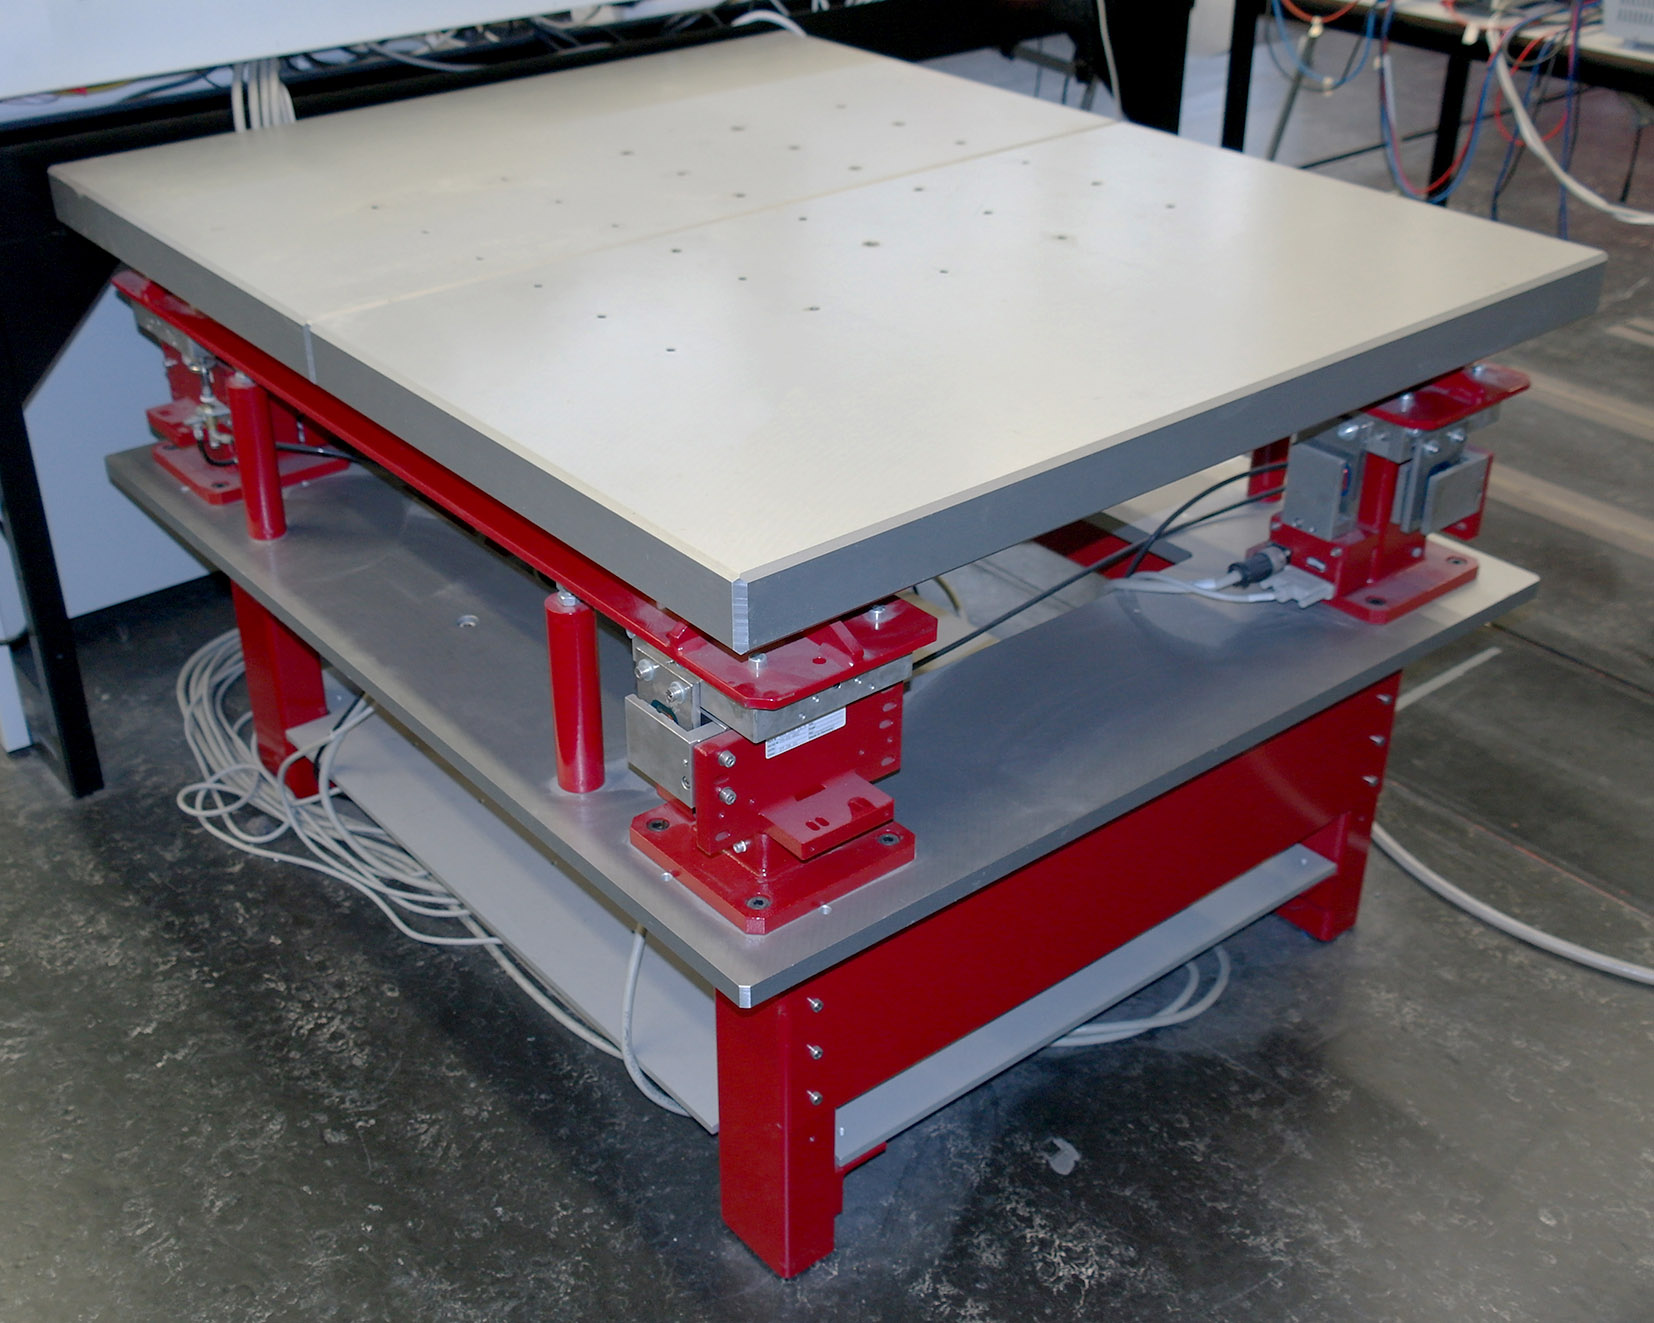
\includegraphics[width=\figurewidth]{\thisDir/figs/avis.jpg}}
  \caption{\Glsentryfirst{AVIS}.}
  \label{fig:lrmhinf:avis}
\end{figure}

\begin{figure}[p]
  \centering
  \setlength{\figurewidth}{0.475\columnwidth}
  \photobox{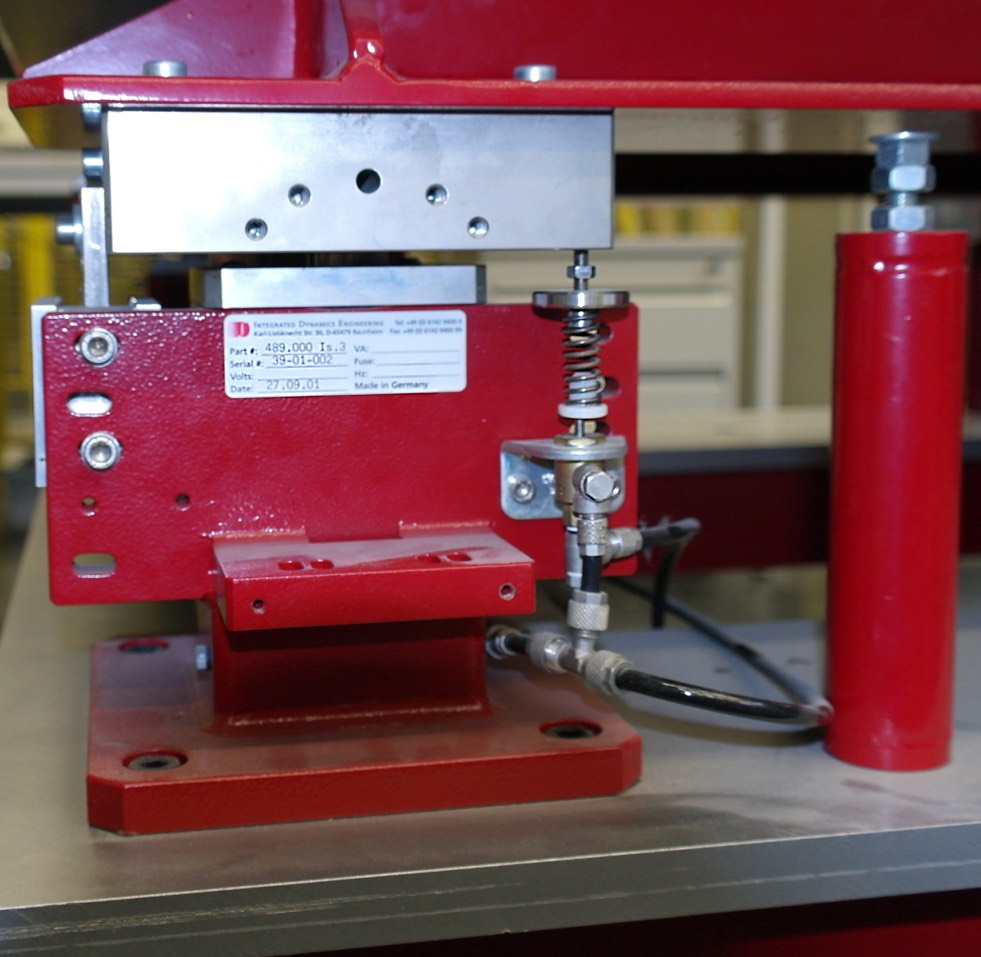
\includegraphics[width=\figurewidth]{\thisDir/figs/avis-airmount-cropped.jpg}}
  \hfill
  \photobox{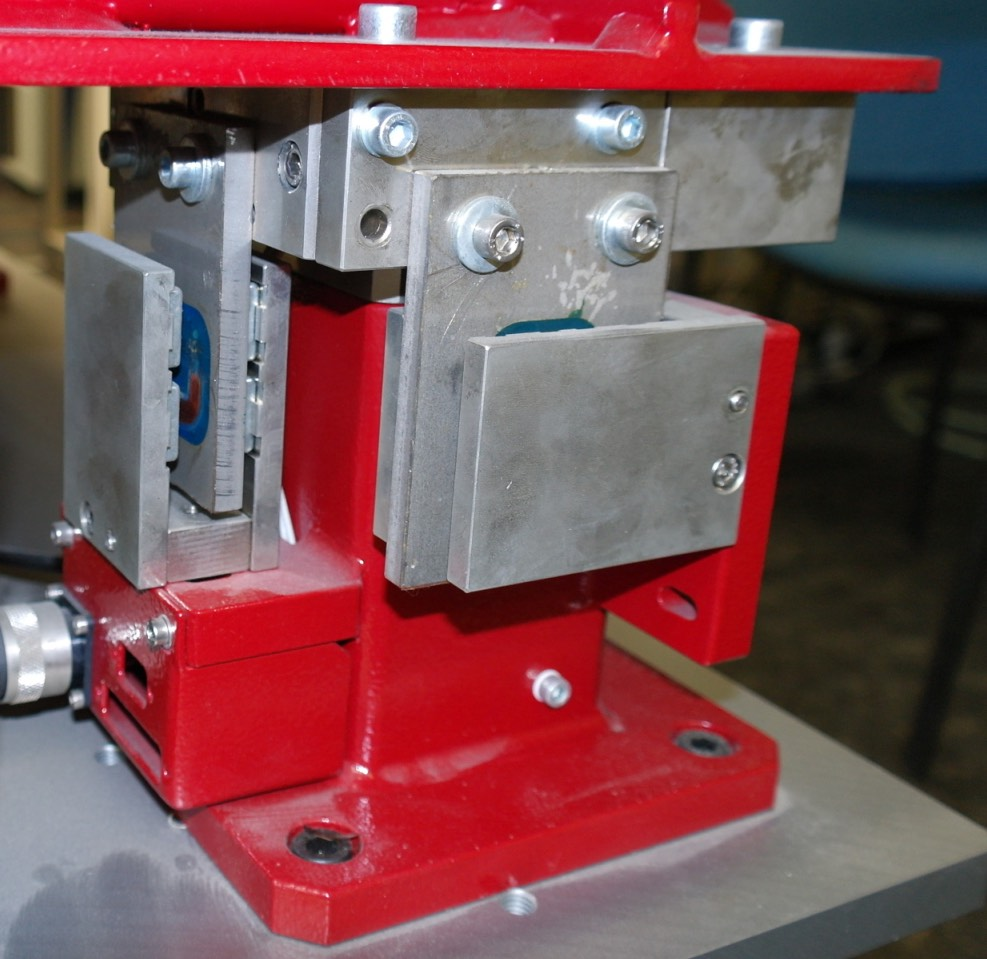
\includegraphics[width=1.005\figurewidth]{\thisDir/figs/avis-motors-cropped.jpg}}
  \caption[\glsentryshort{AVIS} isolation module.]{Isolation module of the \glsentrytext{AVIS}. 
  The left photo shows one of the air mounts providing passive vibration isolation.
  The right photo shows two linear motors that play a role in the active vibration isolation.}
  \label{fig:lrmhinf:avis:details}
\end{figure}

\subsection{Measurement \& Control Framework}
\label{sec:lrmhinf:control}
The experiments on the \gls{AVIS} are carried out in closed-loop (\figref{fig:lrmhinf:tpc}) with $r_2 = 0$.
The controller $\Controller=\experimental\Controller$ is a diagonal \gls{PI} regulator which stabilizes the \gls{AVIS} but yields only moderate vibration isolation.
See \appref{app:avis-setup} for detailed information regarding both the experimental setup and the experimental controller.
The $r_1$ input consists of five periods of a random phase multisine of $65\,536$ samples with excited bins such that $\omega_k \approx 1.001 \omega_{k-1}$  and $\Ts=1\unit{ms}$.
See \chapref{sec:excitation} and \citep{Geerardyn2013TIM} for more information regarding the design of such a signal.

\begin{figure}
 \centering
 \begin{tikzpicture}[scale=1,auto, >=stealth]
    \matrix[ampersand replacement=\&, row sep=0.3cm, column sep=0.6cm] {
%% FIRST ROW
        \node (r1) {$r_1$}; \&
        \&
        \&
        \&
        \node (guide) {}; \&
        \&
        \&
        \&
        \node        (uout) {$u$};  \\
%% SECOND ROW
        \node         (r2) {$r_2$}; \&
        \&
        \node[sum]    (sum2)  {};   \&
        \node[block]  (C)  {$C$};   \&
        \node[sum]    (sum1)  {};   \&
        \node[branch] (u)  {};      \&
        \node[block,color=modelset]  (P)  {$\ModelSet$};   \&
        \node[branch] (y)  {};      \&
        \node       (yout) {$y$};   \\
    };

    \draw [connector] (r2)   -- (sum2);
    \draw [connector] (sum2) -- node {$e_{\vphantom{c}}$}  (C);
    \draw [connector] (C)    -- node {$u_c$}  (sum1);
    \draw [connector] (sum1) -- (P);
    \draw [connector] (P)    -- (yout);
    \draw [connector] (r1)   -| (sum1);
    \draw [connector] (u)    |- (uout);
    \draw [connector] (y)    -- ++(0,-2em) -| node[near end,name=min] {\rotatebox{90}{$-$}} (sum2);

   \begin{pgfonlayer}{background}
     \node[groupbox=TPC, fit=(sum2) (y) (C) (min) (guide)] (TPC) {};
     \node at (TPC.north) [color=TPC, above] {$\ClosedLoop{\ModelSet[],\Controller}$};
   \end{pgfonlayer}

  \end{tikzpicture}

 \caption[Closed-loop block schematic.]{The considered feedback configuration $\ClosedLoop{\ModelSet[],\Controller}$.}
 \label{fig:lrmhinf:tpc}
\end{figure}

\begin{figure}
 \centering
 \begin{tikzpicture}[scale=1, >=stealth]
    \matrix[ampersand replacement=\&, row sep=0.2cm, column sep=0.32cm] {
%% FIRST ROW
        \node        (r1)   {$r_1$};              \&[-0.5em]
        \&
        \&
        \&
        \&
        \&
        \&
        \node[block] (NCp)   {$N_c$};              \&[-0.5em]
        \&[-0.5em]
        \node[block] (DCp)   {$D_c$};              \\
%% SECOND ROW
        \&
        \&
        \&
        \&
        \&
        \&
        \&
        \&
        \node[block] (Delta) {$\Delta$};          \\
%% THIRD ROW
        \node         (r2)   {$r_2$};             \&
        \&
        \node[sum]    (sum2) {};                  \&
        \node[block]  (DC)   {$D_c^{-1}$};        \&
        \node[block]  (NC)   {$N_c$};             \&
        \node[sum]    (sum1) {};                  \&
        \node[sum]    (u)    {};                  \&
        \node[block]  (DP)   {$\hat{D}^ {-1}$};   \&
        \&
        \node[block]  (NP)   {$\hat{N}$};         \&
        \node[sum]    (y)    {};                  \&
        \node         (yout) {$y$};               \\
    };

    \draw [connector] (r1)   -| (sum1);

    \draw [connector] (r2)   -- (sum2);
    \draw [connector] (sum2) -- (DC);
    \draw [connector] (DC)   -- (NC);
    \draw [connector] (NC)   -- (sum1);
    \draw [connector] (sum1) --  node[pos=0.3,above] {$u$} (u);
    \draw [connector] (u)    -- (DP);
    \draw [connector] (DP)   -- (NP);
    \draw [connector] (NP)   -- (y);
    
    \draw [connector] (y)    -- (yout);
    
    \draw [connector] (DP)    -| node [below,name=ud] {$u_{\Delta}$} (Delta);
    \draw [connector] (Delta) |- node [above,name=yd] {$y_{\Delta}$} (DCp) ;
    \draw [connector] (Delta) |- (NCp) ;
    \draw [connector] (DCp)   -| (y) ;
    \draw [connector] (NCp)   -| (u) ;

    \draw [connector] (y) -- ++(0.5em,0) -- ++(0,-2em) -| node[near end,left] {\rotatebox{90}{$-$}} (sum2);

    \begin{pgfonlayer}{background}

      \node[groupbox=controller,fit=(NC) (DC)]                            (C) {};
      \node[groupbox=plant,fit=(NP) (DP)]                           (P) {};
      \node[groupbox=plantset,fit=(P) (Delta) (DCp) (NCp) (y) (u)] (setP) {};

      \node at (C.north)      [color=controller, above]   {$C$};
      \node at (P.north west) [color=plant, above]  {$\hat{P}$};
      \node at (setP.north)   [color=plantset, above] {$\mathcal{P}$};

    \end{pgfonlayer}
\end{tikzpicture}

 \caption[Dual-Youla parametrization.]{Dual-Youla parametrization of the closed-loop set-up  with controller $\Controller$,  model set $\ModelSet[]$ and nominal plant model $\estimated\Plant$.}
\label{fig:lrmhinf:dualYoula}
\end{figure}

The parametrization of the plant model set $\ModelSet[]$ conforms to the dual-\YK{} framework~\citep{Hansen1989,Anderson1998} that parametrizes $\ModelSet[]$ in terms of  all plants $P$ that are stabilized by the controller $C$:
\begin{equation}
  \ModelSet[] 
    \isdef 
      \Set{
            \frac{\hat{N} + D_c \Delta}
                 {\hat{D} - N_c \Delta} 
          |
            \infnorm{\Delta} \leq \gamma
        }
  \label{eq:lrmhinf:dualYoulaModelSet}
  \text{,}
\end{equation}
where $C=N_c D_c^{-1}$ and $\estimated\Plant = \estimated{N}\estimated{D}^{-1}$ are decomposed as \gls{RCF} (see \figref{fig:lrmhinf:dualYoula}).
To estimate $\Delta$ and $\infnorm{\Delta}$, the signals $u_{\Delta}$ and $y_{\Delta}$ in~\figref{fig:lrmhinf:dualYoula} are required.
These can be computed from $u$ and $y$ directly~\citep{Anderson1998}:
\begin{align}
  u_{\Delta}(t) &= \left(\hat{D} + C \hat{N} \right)^{-1} \mat{C & \I} \mat{y(t)\\u(t)}\\
  y_{\Delta}(t) &= \left(D_c + \hat{P} N_c \right)^{-1} \mat{\I & -\hat{P}} \mat{y(t)\\u(t)}
\end{align}
In addition, $u_{\Delta}$ is noise free under standard assumptions~\citep{Hansen1989} and uncorrelated to $y_{\Delta}$. 
Hence the method of \secref{sec:lrmhinf:LPMHinf} applies directly.

The non-uniqueness of the \gls{RCF} can be exploited to satisfy additional conditions.
In view of the robust control criterion
\begin{equation}
  \Crit(\Plant,\Controller) 
    \isdef 
      \infnorm{W \ClosedLoop{\Plant,\Controller} V}
  \label{eq:lrmhinf:controlCrit}
  \text{,}
\end{equation}
the \glspl{RCF} are constructed such that
$
  \worstCase\Crit \left( \ModelSet[], \experimental\Controller \right)
  \leq
  \Crit \left( \estimated\Plant, \experimental\Controller \right)
  + \gamma
$
where $\worstCase\Crit(\ModelSet[],C) \isdef \sup_{P\in\ModelSet[]} \Crit(P,C)$~\citep{Oomen2012SIRP}.
% Obviously, $\Crit( \true\Plant, \experimental\Controller) \leq \worstCase\Crit ( \ModelSet[], \experimental\Controller )$ is guaranteed when $\true\Plant \in \ModelSet[]$.
I.e. even for a weighted control criterion \eqref{eq:lrmhinf:controlCrit}, there is no need to incorporate weights $W'$ and $V'$ into the estimation of the uncertainty bound as $\infnorm{W' \Delta V'}$.
In this chapter, an eighth-order $\estimated\Plant$~(\figref{fig:lrmhinf:avis-frf}) is estimated.
Some dynamics are left unmodeled and are hence part of $\Delta$~(\figref{fig:lrmhinf:avisMeas}).

\begin{figure}
 \centering
    \setlength{\figurewidth}{0.75\columnwidth}
    \setlength{\figureheight}{0.68\figurewidth}
    % This file was created by matlab2tikz v0.4.3 (commit 2110609f2d993ab5074ce6b8f3e699d75d77a6b6).
% Copyright (c) 2008--2013, Nico Schlömer <nico.schloemer@gmail.com>
% All rights reserved.
% 
% The latest updates can be retrieved from
%   http://www.mathworks.com/matlabcentral/fileexchange/22022-matlab2tikz
% where you can also make suggestions and rate matlab2tikz.
% 
\begin{tikzpicture}

\begin{axis}[%
width=\figurewidth,
height=\figureheight,
scale only axis,
xmode=log,
xmin=9.9,
xmax=500,
ymajorgrids,
xmajorgrids,
xminorgrids,
xminorticks=true,
ymin=-70,
ymax=16,
ylabel={Amplitude $\abs{P}$ \axisunit{dB}},
xlabel={Frequency $\omega$  \axisunit{Hz}},
name=plot0
]

\addplot [paramPhat]
table[row sep=crcr] {
% 0.0152587890625 23.7722447525977\\
% 0.0457763671875 22.3080847897672\\
% 0.0762939453125 20.2741569707957\\
% 0.1068115234375 18.2257529897462\\
% 0.1373291015625 16.3079974146639\\
% 0.1678466796875 14.5181085972517\\
% 0.1983642578125 12.8172522087776\\
% 0.2288818359375 11.1608733787134\\
% 0.2593994140625 9.50397723607956\\
% 0.2899169921875 7.79899510770321\\
% 0.3204345703125 5.99029715556577\\
% 0.3509521484375 4.00469298301403\\
% 0.3814697265625 1.73365389099158\\
% 0.4119873046875 -1.00426577865468\\
% 0.4425048828125 -4.54966533123516\\
% 0.4730224609375 -9.51643537709583\\
% 0.5035400390625 -13.8964915122691\\
% 0.5340576171875 -9.50421779076407\\
% 0.5645751953125 -5.12612382304163\\
% 0.5950927734375 -2.12859036094432\\
% 0.6256103515625 0.0795243024252674\\
% 0.6561279296875 1.81283230611915\\
% 0.6866455078125 3.23551080308591\\
% 0.7171630859375 4.44140167314812\\
% 0.7476806640625 5.48852713143906\\
% 0.7781982421875 6.41503322856487\\
% 0.8087158203125 7.24723490797363\\
% 0.8392333984375 8.00399673011526\\
% 0.8697509765625 8.69927256044658\\
% 0.9002685546875 9.34365587383497\\
% 0.9307861328125 9.94536758467433\\
% 0.9613037109375 10.5109086205\\
% 0.9918212890625 11.0455044893486\\
% 1.0223388671875 11.5534162767064\\
% 1.0528564453125 12.0381632797992\\
% 1.0833740234375 12.5026856473201\\
% 1.1138916015625 12.9494653430929\\
% 1.1444091796875 13.3806175660085\\
% 1.1749267578125 13.7979608445429\\
% 1.2054443359375 14.2030714862825\\
% 1.2359619140625 14.5973263807037\\
% 1.2664794921875 14.9819370161158\\
% 1.2969970703125 15.3579767887555\\
% 1.3275146484375 15.7264031341724\\
% 1.3580322265625 16.0880756219148\\
% 1.3885498046875 16.4437708743058\\
% 1.4190673828125 16.7941949657516\\
% 1.4495849609375 17.1399938082556\\
% 1.4801025390625 17.4817619163763\\
% 1.5106201171875 17.8200498601774\\
% 1.5411376953125 18.1553706503383\\
% 1.5716552734375 18.4882052502356\\
% 1.6021728515625 18.8190073716575\\
% 1.6326904296875 19.1482076811222\\
% 1.6632080078125 19.4762175204909\\
% 1.6937255859375 19.8034322272109\\
% 1.7242431640625 20.1302341249468\\
% 1.7547607421875 20.4569952437229\\
% 1.7852783203125 20.7840798193475\\
% 1.8157958984375 21.1118466143154\\
% 1.8463134765625 21.4406510961916\\
% 1.8768310546875 21.7708475043434\\
% 1.9073486328125 22.1027908315403\\
% 1.9378662109375 22.4368387431394\\
% 1.9683837890625 22.7733534531064\\
% 1.9989013671875 23.112703572744\\
% 2.0294189453125 23.4552659444922\\
% 2.0599365234375 23.8014274692076\\
% 2.0904541015625 24.1515869305938\\
% 2.1209716796875 24.5061568144554\\
% 2.1514892578125 24.8655651125802\\
% 2.1820068359375 25.2302570904768\\
% 2.2125244140625 25.600696983754\\
% 2.2430419921875 25.9773695680442\\
% 2.2735595703125 26.3607815198056\\
% 2.3040771484375 26.7514624470049\\
% 2.3345947265625 27.1499654151986\\
% 2.3651123046875 27.556866719776\\
% 2.3956298828125 27.9727645504501\\
% 2.4261474609375 28.398276047329\\
% 2.4566650390625 28.8340320419987\\
% 2.4871826171875 29.2806684882203\\
% 2.5177001953125 29.738813182202\\
% 2.5482177734375 30.2090658074338\\
% 2.5787353515625 30.6919685550836\\
% 2.6092529296875 31.1879634947029\\
% 2.6397705078125 31.6973314186676\\
% 2.6702880859375 32.2201049841374\\
% 2.7008056640625 32.7559466142805\\
% 2.7313232421875 33.3039789538858\\
% 2.7618408203125 33.8625532646832\\
% 2.7923583984375 34.4289403934151\\
% 2.8228759765625 34.998932818317\\
% 2.8533935546875 35.5663602956612\\
% 2.8839111328125 36.1225545670644\\
% 2.9144287109375 36.6558610950166\\
% 2.9449462890625 37.1513927585097\\
% 2.9754638671875 37.5913317342492\\
% 3.0059814453125 37.9561374983115\\
% 3.0364990234375 38.2268760492636\\
% 3.0670166015625 38.388435532638\\
% 3.0975341796875 38.4327465267617\\
% 3.1280517578125 38.3607353513796\\
% 3.1585693359375 38.1820974821149\\
% 3.1890869140625 37.9130018010624\\
% 3.2196044921875 37.5727752169157\\
% 3.2501220703125 37.1808111366764\\
% 3.2806396484375 36.7544592218602\\
% 3.3111572265625 36.3080196085472\\
% 3.3416748046875 35.8525763470607\\
% 3.3721923828125 35.3963117506141\\
% 3.4027099609375 34.9450157498753\\
% 3.4332275390625 34.5026165737593\\
% 3.4637451171875 34.0716497331852\\
% 3.4942626953125 33.6536382712904\\
% 3.5247802734375 33.249385659551\\
% 3.5552978515625 32.8591941702117\\
% 3.5858154296875 32.4830241866703\\
% 3.6163330078125 32.1206086666063\\
% 3.6468505859375 31.771534437305\\
% 3.6773681640625 31.4352993686595\\
% 3.7078857421875 31.1113521929172\\
% 3.7384033203125 30.7991199322042\\
% 3.7689208984375 30.4980265233318\\
% 3.7994384765625 30.2075052166461\\
% 3.8299560546875 29.9270065898856\\
% 3.8604736328125 29.6560034886193\\
% 3.8909912109375 29.3939938260787\\
% 3.9215087890625 29.1405019050057\\
% 3.9520263671875 28.8950787316553\\
% 3.9825439453125 28.6573016549751\\
% 4.0130615234375 28.4267735662919\\
% 4.0435791015625 28.2031218251764\\
% 4.0740966796875 27.9859970274679\\
% 4.1046142578125 27.775071695985\\
% 4.1351318359375 27.5700389491584\\
% 4.1656494140625 27.3706111848061\\
% 4.1961669921875 27.1765188034565\\
% 4.2266845703125 26.9875089865579\\
% 4.2572021484375 26.8033445385226\\
% 4.2877197265625 26.6238027970888\\
% 4.3182373046875 26.448674613411\\
% 4.3487548828125 26.2777634012001\\
% 4.3792724609375 26.1108842528586\\
% 4.4097900390625 25.9478631196883\\
% 4.4403076171875 25.7885360527342\\
% 4.4708251953125 25.6327485005659\\
% 4.5013427734375 25.4803546602147\\
% 4.5318603515625 25.3312168775128\\
% 4.5623779296875 25.1852050931961\\
% 4.5928955078125 25.0421963312868\\
% 4.6234130859375 24.9020742264696\\
% 4.6539306640625 24.7647285873746\\
% 4.6844482421875 24.6300549928949\\
% 4.7149658203125 24.4979544188742\\
% 4.7454833984375 24.3683328927045\\
% 4.7760009765625 24.2411011735653\\
% 4.8065185546875 24.1161744562232\\
% 4.8370361328125 23.9934720964781\\
% 4.8675537109375 23.8729173565049\\
% 4.8980712890625 23.7544371684859\\
% 4.9285888671875 23.6379619150655\\
% 4.9591064453125 23.5234252252845\\
% 4.9896240234375 23.4107637847641\\
% 5.0201416015625 23.2999171590175\\
% 5.0506591796875 23.1908276288606\\
% 5.0811767578125 23.0834400369808\\
% 5.1116943359375 22.9777016448047\\
% 5.1422119140625 22.8735619988752\\
% 5.1727294921875 22.7709728060182\\
% 5.2032470703125 22.6698878166361\\
% 5.2337646484375 22.5702627155228\\
% 5.2642822265625 22.4720550196442\\
% 5.2947998046875 22.3752239823726\\
% 5.3253173828125 22.2797305037082\\
% 5.3558349609375 22.1855370460544\\
% 5.3863525390625 22.0926075551535\\
% 5.4168701171875 22.0009073858157\\
% 5.4473876953125 21.9104032321067\\
% 5.4779052734375 21.8210630616861\\
% 5.5084228515625 21.7328560540075\\
% 5.5389404296875 21.6457525421218\\
% 5.5694580078125 21.5597239578368\\
% 5.5999755859375 21.4747427800109\\
% 5.6304931640625 21.3907824857722\\
% 5.6610107421875 21.3078175044717\\
% 5.6915283203125 21.2258231741913\\
% 5.7220458984375 21.1447757006444\\
% 5.7525634765625 21.0646521183131\\
% 5.7830810546875 20.9854302536835\\
% 5.8135986328125 20.9070886904451\\
% 5.8441162109375 20.8296067365336\\
% 5.8746337890625 20.7529643929023\\
% 5.9051513671875 20.6771423239184\\
% 5.9356689453125 20.6021218292832\\
% 5.9661865234375 20.5278848173871\\
% 5.9967041015625 20.4544137800129\\
% 6.0272216796875 20.3816917683075\\
% 6.0577392578125 20.3097023699493\\
% 6.0882568359375 20.2384296874399\\
% 6.1187744140625 20.1678583174577\\
% 6.1492919921875 20.0979733312107\\
% 6.1798095703125 20.0287602557339\\
% 6.2103271484375 19.9602050560772\\
% 6.2408447265625 19.8922941183343\\
% 6.2713623046875 19.8250142334668\\
% 6.3018798828125 19.7583525818799\\
% 6.3323974609375 19.6922967187082\\
% 6.3629150390625 19.6268345597746\\
% 6.3934326171875 19.5619543681849\\
% 6.4239501953125 19.4976447415258\\
% 6.4544677734375 19.4338945996339\\
% 6.4849853515625 19.370693172906\\
% 6.5155029296875 19.3080299911225\\
% 6.5460205078125 19.2458948727579\\
% 6.5765380859375 19.1842779147538\\
% 6.6070556640625 19.1231694827303\\
% 6.6375732421875 19.0625602016145\\
% 6.6680908203125 19.0024409466643\\
% 6.6986083984375 18.9428028348697\\
% 6.7291259765625 18.8836372167118\\
% 6.7596435546875 18.8249356682611\\
% 6.7901611328125 18.7666899836022\\
% 6.8206787109375 18.7088921675647\\
% 6.8511962890625 18.6515344287496\\
% 6.8817138671875 18.5946091728347\\
% 6.9122314453125 18.5381089961471\\
% 6.9427490234375 18.4820266794898\\
% 6.9732666015625 18.4263551822117\\
% 7.0037841796875 18.3710876365075\\
% 7.0343017578125 18.3162173419396\\
% 7.0648193359375 18.2617377601706\\
% 7.0953369140625 18.2076425098967\\
% 7.1258544921875 18.1539253619737\\
% 7.1563720703125 18.1005802347269\\
% 7.1868896484375 18.0476011894361\\
% 7.2174072265625 17.9949824259891\\
% 7.2479248046875 17.9427182786955\\
% 7.2784423828125 17.8908032122542\\
% 7.3089599609375 17.8392318178679\\
% 7.3394775390625 17.7879988094988\\
% 7.3699951171875 17.7370990202583\\
% 7.4005126953125 17.6865273989263\\
% 7.4310302734375 17.6362790065947\\
% 7.4615478515625 17.5863490134282\\
% 7.4920654296875 17.5367326955395\\
% 7.5225830078125 17.487425431974\\
% 7.5531005859375 17.4384227017976\\
% 7.5836181640625 17.389720081286\\
% 7.6141357421875 17.3413132412099\\
% 7.6446533203125 17.2931979442118\\
% 7.6751708984375 17.2453700422729\\
% 7.7056884765625 17.1978254742634\\
% 7.7362060546875 17.1505602635765\\
% 7.7667236328125 17.1035705158395\\
% 7.7972412109375 17.0568524167007\\
% 7.8277587890625 17.0104022296899\\
% 7.8582763671875 16.9642162941472\\
% 7.8887939453125 16.9182910232204\\
% 7.9193115234375 16.8726229019257\\
% 7.9498291015625 16.8272084852716\\
% 7.9803466796875 16.7820443964416\\
% 8.0108642578125 16.7371273250358\\
% 8.0413818359375 16.6924540253663\\
% 8.0718994140625 16.6480213148072\\
% 8.1024169921875 16.6038260721958\\
% 8.1329345703125 16.5598652362826\\
% 8.1634521484375 16.5161358042302\\
% 8.1939697265625 16.472634830157\\
% 8.2244873046875 16.4293594237263\\
% 8.2550048828125 16.3863067487773\\
% 8.2855224609375 16.3434740219981\\
% 8.3160400390625 16.3008585116377\\
% 8.3465576171875 16.2584575362571\\
% 8.3770751953125 16.2162684635168\\
% 8.4075927734375 16.1742887090009\\
% 8.4381103515625 16.1325157350745\\
% 8.4686279296875 16.0909470497756\\
% 8.4991455078125 16.0495802057382\\
% 8.5296630859375 16.0084127991474\\
% 8.5601806640625 15.9674424687237\\
% 8.5906982421875 15.9266668947367\\
% 8.6212158203125 15.8860837980471\\
% 8.6517333984375 15.8456909391749\\
% 8.6822509765625 15.8054861173949\\
% 8.7127685546875 15.7654671698568\\
% 8.7432861328125 15.72563197073\\
% 8.7738037109375 15.685978430372\\
% 8.8043212890625 15.6465044945199\\
% 8.8348388671875 15.6072081435041\\
% 8.8653564453125 15.5680873914829\\
% 8.8958740234375 15.529140285699\\
% 8.9263916015625 15.4903649057547\\
% 8.9569091796875 15.4517593629078\\
% 8.9874267578125 15.4133217993855\\
% 9.0179443359375 15.3750503877171\\
% 9.0484619140625 15.3369433300839\\
% 9.0789794921875 15.298998857687\\
% 9.1094970703125 15.2612152301306\\
% 9.1400146484375 15.2235907348225\\
% 9.1705322265625 15.1861236863892\\
% 9.2010498046875 15.1488124261069\\
% 9.2315673828125 15.111655321347\\
% 9.2620849609375 15.0746507650352\\
% 9.2926025390625 15.0377971751251\\
% 9.3231201171875 15.001092994085\\
% 9.3536376953125 14.9645366883972\\
% 9.3841552734375 14.9281267480708\\
% 9.4146728515625 14.8918616861655\\
% 9.4451904296875 14.8557400383283\\
% 9.4757080078125 14.8197603623414\\
% 9.5062255859375 14.7839212376807\\
% 9.5367431640625 14.748221265086\\
% 9.5672607421875 14.7126590661409\\
% 9.5977783203125 14.677233282864\\
% 9.6282958984375 14.6419425773086\\
% 9.6588134765625 14.6067856311732\\
% 9.6893310546875 14.5717611454208\\
% 9.7198486328125 14.5368678399078\\
% 9.7503662109375 14.5021044530208\\
9.7808837890625 14.4674697413231\\
9.8114013671875 14.4329624792088\\
9.8419189453125 14.3985814585653\\
9.8724365234375 14.3643254884439\\
9.9029541015625 14.3301933947372\\
9.9334716796875 14.2961840198655\\
9.9639892578125 14.2622962224688\\
9.9945068359375 14.228528877107\\
10.0250244140625 14.1948808739665\\
10.0555419921875 14.1613511185736\\
10.0860595703125 14.1279385315143\\
10.1165771484375 14.0946420481607\\
10.1470947265625 14.0614606184031\\
10.1776123046875 14.0283932063886\\
10.2081298828125 13.9954387902654\\
10.2386474609375 13.9625963619322\\
10.2691650390625 13.9298649267941\\
10.2996826171875 13.8972435035233\\
10.3302001953125 13.8647311238251\\
10.3607177734375 13.8323268322089\\
10.3912353515625 13.8000296857646\\
10.4217529296875 13.7678387539438\\
10.4522705078125 13.7357531183448\\
10.4827880859375 13.7037718725037\\
10.5133056640625 13.6718941216888\\
10.5438232421875 13.6401189826999\\
10.5743408203125 13.6084455836716\\
10.6048583984375 13.5768730638813\\
10.6353759765625 13.5454005735605\\
10.6658935546875 13.5140272737106\\
10.6964111328125 13.4827523359222\\
10.7269287109375 13.4515749421985\\
10.7574462890625 13.4204942847822\\
10.7879638671875 13.3895095659856\\
10.8184814453125 13.3586199980252\\
10.8489990234375 13.3278248028585\\
10.8795166015625 13.2971232120247\\
10.9100341796875 13.266514466489\\
10.9405517578125 13.2359978164894\\
10.9710693359375 13.2055725213867\\
11.0015869140625 13.175237849518\\
11.0321044921875 13.1449930780526\\
11.0626220703125 13.1148374928508\\
11.0931396484375 13.0847703883262\\
11.1236572265625 13.0547910673096\\
11.1541748046875 13.0248988409165\\
11.1846923828125 12.9950930284171\\
11.2152099609375 12.9653729571079\\
11.2457275390625 12.9357379621872\\
11.2762451171875 12.9061873866321\\
11.3067626953125 12.876720581078\\
11.3372802734375 12.847336903701\\
11.3677978515625 12.8180357201012\\
11.3983154296875 12.7888164031902\\
11.4288330078125 12.7596783330788\\
11.4593505859375 12.7306208969682\\
11.4898681640625 12.7016434890426\\
11.5203857421875 12.6727455103641\\
11.5509033203125 12.643926368769\\
11.5814208984375 12.6151854787671\\
11.6119384765625 12.5865222614421\\
11.6424560546875 12.5579361443536\\
11.6729736328125 12.529426561442\\
11.7034912109375 12.5009929529339\\
11.7340087890625 12.4726347652501\\
11.7645263671875 12.444351450915\\
11.7950439453125 12.4161424684678\\
11.8255615234375 12.3880072823747\\
11.8560791015625 12.3599453629436\\
11.8865966796875 12.3319561862398\\
11.9171142578125 12.3040392340031\\
11.9476318359375 12.276193993567\\
11.9781494140625 12.2484199577786\\
12.0086669921875 12.2207166249204\\
12.0391845703125 12.1930834986332\\
12.0697021484375 12.1655200878409\\
12.1002197265625 12.1380259066756\\
12.1307373046875 12.1106004744055\\
12.1612548828125 12.0832433153624\\
12.1917724609375 12.0559539588717\\
12.2222900390625 12.0287319391832\\
12.2528076171875 12.0015767954029\\
12.2833251953125 11.9744880714262\\
12.3138427734375 11.9474653158724\\
12.3443603515625 11.92050808202\\
12.3748779296875 11.8936159277431\\
12.4053955078125 11.8667884154491\\
12.4359130859375 11.8400251120177\\
12.4664306640625 11.8133255887401\\
12.4969482421875 11.7866894212599\\
12.5274658203125 11.7601161895151\\
12.5579833984375 11.7336054776803\\
12.5885009765625 11.7071568741107\\
12.6190185546875 11.6807699712867\\
12.6495361328125 11.6544443657591\\
12.6800537109375 11.6281796580957\\
12.7105712890625 11.6019754528288\\
12.7410888671875 11.5758313584027\\
12.7716064453125 11.5497469871235\\
12.8021240234375 11.5237219551083\\
12.8326416015625 11.4977558822361\\
12.8631591796875 11.4718483920992\\
12.8936767578125 11.4459991119555\\
12.9241943359375 11.4202076726812\\
12.9547119140625 11.3944737087249\\
12.9852294921875 11.368796858062\\
13.0157470703125 11.3431767621495\\
13.0462646484375 11.3176130658826\\
13.0767822265625 11.2921054175508\\
13.1072998046875 11.2666534687952\\
13.1378173828125 11.241256874567\\
13.1683349609375 11.2159152930852\\
13.1988525390625 11.190628385797\\
13.2293701171875 11.1653958173365\\
13.2598876953125 11.1402172554864\\
13.2904052734375 11.1150923711383\\
13.3209228515625 11.0900208382547\\
13.3514404296875 11.0650023338314\\
13.3819580078125 11.0400365378604\\
13.4124755859375 11.0151231332933\\
13.4429931640625 10.9902618060052\\
13.4735107421875 10.9654522447596\\
13.5040283203125 10.9406941411732\\
13.5345458984375 10.9159871896818\\
13.5650634765625 10.8913310875061\\
13.5955810546875 10.8667255346189\\
13.6260986328125 10.8421702337115\\
13.6566162109375 10.8176648901621\\
13.6871337890625 10.7932092120036\\
13.7176513671875 10.768802909892\\
13.7481689453125 10.7444456970759\\
13.7786865234375 10.7201372893656\\
13.8092041015625 10.6958774051034\\
13.8397216796875 10.6716657651338\\
13.8702392578125 10.6475020927743\\
13.9007568359375 10.6233861137871\\
13.9312744140625 10.5993175563502\\
13.9617919921875 10.5752961510297\\
13.9923095703125 10.5513216307524\\
14.0228271484375 10.5273937307787\\
14.0533447265625 10.5035121886758\\
14.0838623046875 10.4796767442912\\
14.1143798828125 10.455887139727\\
14.1448974609375 10.4321431193141\\
14.1754150390625 10.4084444295873\\
14.2059326171875 10.3847908192599\\
14.2364501953125 10.3611820391997\\
14.2669677734375 10.3376178424043\\
14.2974853515625 10.3140979839777\\
14.3280029296875 10.2906222211067\\
14.3585205078125 10.2671903130375\\
14.3890380859375 10.2438020210529\\
14.4195556640625 10.22045710845\\
14.4500732421875 10.1971553405177\\
14.4805908203125 10.1738964845149\\
14.5111083984375 10.1506803096488\\
14.5416259765625 10.1275065870537\\
14.5721435546875 10.1043750897697\\
14.6026611328125 10.0812855927223\\
14.6331787109375 10.0582378727017\\
14.6636962890625 10.0352317083424\\
14.6942138671875 10.012266880104\\
14.7247314453125 9.98934317025066\\
14.7552490234375 9.96646036283231\\
14.7857666015625 9.9436182436653\\
14.8162841796875 9.92081660031357\\
14.8468017578125 9.89805522207\\
14.8773193359375 9.87533389993805\\
14.9078369140625 9.85265242661365\\
14.9383544921875 9.83001059646725\\
14.9688720703125 9.80740820552622\\
14.9993896484375 9.78484505145737\\
15.0299072265625 9.7623209335498\\
15.0604248046875 9.73983565269793\\
15.0909423828125 9.71738901138468\\
15.1214599609375 9.69498081366498\\
15.1519775390625 9.6726108651495\\
15.1824951171875 9.65027897298842\\
15.2130126953125 9.62798494585566\\
15.2435302734375 9.60572859393307\\
15.2740478515625 9.583509728895\\
15.3045654296875 9.561328163893\\
15.3350830078125 9.53918371354067\\
15.3656005859375 9.5170761938988\\
15.3961181640625 9.49500542246062\\
15.4266357421875 9.47297121813725\\
15.4571533203125 9.45097340124339\\
15.4876708984375 9.42901179348313\\
15.5181884765625 9.40708621793591\\
15.5487060546875 9.38519649904277\\
15.5792236328125 9.36334246259269\\
15.6097412109375 9.34152393570905\\
15.6402587890625 9.31974074683639\\
15.6707763671875 9.29799272572725\\
15.7012939453125 9.27627970342915\\
15.7318115234375 9.25460151227182\\
15.7623291015625 9.23295798585454\\
15.7928466796875 9.21134895903353\\
15.8233642578125 9.1897742679097\\
15.8538818359375 9.16823374981642\\
15.8843994140625 9.14672724330747\\
15.9149169921875 9.12525458814505\\
15.9454345703125 9.10381562528812\\
15.9759521484375 9.08241019688072\\
16.0064697265625 9.0610381462405\\
16.0369873046875 9.03969931784732\\
16.0675048828125 9.01839355733217\\
16.0980224609375 8.99712071146595\\
16.1285400390625 8.97588062814859\\
16.1590576171875 8.95467315639825\\
16.1895751953125 8.9334981463406\\
16.2200927734375 8.91235544919827\\
16.2506103515625 8.89124491728043\\
16.2811279296875 8.87016640397246\\
16.3116455078125 8.84911976372578\\
16.3421630859375 8.82810485204775\\
16.3726806640625 8.80712152549171\\
16.4031982421875 8.78616964164721\\
16.4337158203125 8.76524905913021\\
16.4642333984375 8.7443596375735\\
16.4947509765625 8.72350123761718\\
16.5252685546875 8.70267372089935\\
16.5557861328125 8.68187695004671\\
16.5863037109375 8.66111078866546\\
16.6168212890625 8.64037510133222\\
16.6473388671875 8.61966975358509\\
16.6778564453125 8.59899461191467\\
16.7083740234375 8.57834954375548\\
16.7388916015625 8.55773441747715\\
16.7694091796875 8.53714910237591\\
16.7999267578125 8.51659346866614\\
16.8304443359375 8.49606738747194\\
16.8609619140625 8.4755707308189\\
16.8914794921875 8.45510337162595\\
16.9219970703125 8.43466518369715\\
16.9525146484375 8.41425604171381\\
16.9830322265625 8.39387582122649\\
17.0135498046875 8.37352439864721\\
17.0440673828125 8.35320165124173\\
17.0745849609375 8.33290745712187\\
17.1051025390625 8.31264169523793\\
17.1356201171875 8.29240424537123\\
17.1661376953125 8.27219498812669\\
17.1966552734375 8.25201380492555\\
17.2271728515625 8.23186057799806\\
17.2576904296875 8.21173519037637\\
17.2882080078125 8.19163752588742\\
17.3187255859375 8.17156746914593\\
17.3492431640625 8.15152490554753\\
17.3797607421875 8.13150972126179\\
17.4102783203125 8.11152180322553\\
17.4407958984375 8.09156103913611\\
17.4713134765625 8.07162731744471\\
17.5018310546875 8.05172052734986\\
17.5323486328125 8.03184055879088\\
17.5628662109375 8.0119873024415\\
17.5933837890625 7.99216064970347\\
17.6239013671875 7.97236049270026\\
17.6544189453125 7.95258672427089\\
17.6849365234375 7.93283923796372\\
17.7154541015625 7.91311792803038\\
17.7459716796875 7.89342268941975\\
17.7764892578125 7.87375341777194\\
17.8070068359375 7.8541100094125\\
17.8375244140625 7.83449236134646\\
17.8680419921875 7.81490037125262\\
17.8985595703125 7.79533393747781\\
17.9290771484375 7.77579295903122\\
17.9595947265625 7.75627733557886\\
17.9901123046875 7.73678696743791\\
18.0206298828125 7.71732175557132\\
18.0511474609375 7.69788160158236\\
18.0816650390625 7.67846640770924\\
18.1121826171875 7.6590760768198\\
18.1427001953125 7.63971051240622\\
18.1732177734375 7.62036961857987\\
18.2037353515625 7.60105330006607\\
18.2342529296875 7.58176146219908\\
18.2647705078125 7.56249401091696\\
18.2952880859375 7.54325085275665\\
18.3258056640625 7.52403189484894\\
18.3563232421875 7.50483704491362\\
18.3868408203125 7.48566621125467\\
18.4173583984375 7.46651930275532\\
18.4478759765625 7.44739622887348\\
18.4783935546875 7.42829689963687\\
18.5089111328125 7.40922122563846\\
18.5394287109375 7.39016911803183\\
18.5699462890625 7.37114048852659\\
18.6004638671875 7.3521352493839\\
18.6309814453125 7.3331533134119\\
18.6614990234375 7.31419459396143\\
18.6920166015625 7.2952590049215\\
18.7225341796875 7.27634646071503\\
18.7530517578125 7.25745687629449\\
18.7835693359375 7.23859016713771\\
18.8140869140625 7.21974624924357\\
18.8446044921875 7.20092503912794\\
18.8751220703125 7.18212645381942\\
18.9056396484375 7.16335041085535\\
18.9361572265625 7.14459682827768\\
18.9666748046875 7.125865624629\\
18.9971923828125 7.10715671894853\\
19.0277099609375 7.08847003076823\\
19.0582275390625 7.06980548010881\\
19.0887451171875 7.05116298747598\\
19.1192626953125 7.03254247385653\\
19.1497802734375 7.01394386071459\\
19.1802978515625 6.99536706998786\\
19.2108154296875 6.97681202408391\\
19.2413330078125 6.95827864587645\\
19.2718505859375 6.93976685870177\\
19.3023681640625 6.92127658635502\\
19.3328857421875 6.90280775308673\\
19.3634033203125 6.88436028359922\\
19.3939208984375 6.86593410304305\\
19.4244384765625 6.84752913701364\\
19.4549560546875 6.82914531154775\\
19.4854736328125 6.81078255312009\\
19.5159912109375 6.79244078863994\\
19.5465087890625 6.7741199454478\\
19.5770263671875 6.75581995131207\\
19.6075439453125 6.73754073442577\\
19.6380615234375 6.71928222340328\\
19.6685791015625 6.70104434727712\\
19.6990966796875 6.68282703549474\\
19.7296142578125 6.66463021791537\\
19.7601318359375 6.64645382480689\\
19.7906494140625 6.6282977868427\\
19.8211669921875 6.61016203509864\\
19.8516845703125 6.59204650104995\\
19.8822021484375 6.57395111656827\\
19.9127197265625 6.55587581391859\\
19.9432373046875 6.53782052575635\\
19.9737548828125 6.51978518512443\\
20.0042724609375 6.50176972545029\\
20.0347900390625 6.48377408054303\\
20.0653076171875 6.46579818459061\\
20.0958251953125 6.44784197215695\\
20.1263427734375 6.42990537817908\\
20.1568603515625 6.41198833796449\\
20.1873779296875 6.39409078718827\\
20.2178955078125 6.37621266189035\\
20.2484130859375 6.3583538984729\\
20.2789306640625 6.34051443369755\\
20.3094482421875 6.32269420468276\\
20.3399658203125 6.30489314890121\\
20.3704833984375 6.28711120417712\\
20.4010009765625 6.26934830868375\\
20.4315185546875 6.25160440094071\\
20.4620361328125 6.23387941981156\\
20.4925537109375 6.21617330450117\\
20.5230712890625 6.19848599455327\\
20.5535888671875 6.18081742984796\\
20.5841064453125 6.16316755059928\\
20.6146240234375 6.14553629735274\\
20.6451416015625 6.12792361098292\\
20.6756591796875 6.11032943269106\\
20.7061767578125 6.09275370400278\\
20.7366943359375 6.07519636676555\\
20.7672119140625 6.05765736314657\\
20.7977294921875 6.04013663563027\\
20.8282470703125 6.02263412701618\\
20.8587646484375 6.00514978041654\\
20.8892822265625 5.98768353925414\\
20.9197998046875 5.97023534726001\\
20.9503173828125 5.95280514847126\\
20.9808349609375 5.93539288722887\\
21.0113525390625 5.91799850817557\\
21.0418701171875 5.90062195625357\\
21.0723876953125 5.88326317670251\\
21.1029052734375 5.86592211505734\\
21.1334228515625 5.8485987171462\\
21.1639404296875 5.83129292908835\\
21.1944580078125 5.81400469729206\\
21.2249755859375 5.79673396845264\\
21.2554931640625 5.77948068955037\\
21.2860107421875 5.76224480784847\\
21.3165283203125 5.74502627089113\\
21.3470458984375 5.72782502650156\\
21.3775634765625 5.71064102277996\\
21.4080810546875 5.69347420810163\\
21.4385986328125 5.67632453111502\\
21.4691162109375 5.65919194073982\\
21.4996337890625 5.64207638616508\\
21.5301513671875 5.62497781684731\\
21.5606689453125 5.6078961825086\\
21.5911865234375 5.59083143313484\\
21.6217041015625 5.57378351897381\\
21.6522216796875 5.55675239053339\\
21.6827392578125 5.53973799857976\\
21.7132568359375 5.52274029413563\\
21.7437744140625 5.50575922847843\\
21.7742919921875 5.48879475313859\\
21.8048095703125 5.47184681989774\\
21.8353271484375 5.45491538078707\\
21.8658447265625 5.43800038808551\\
21.8963623046875 5.42110179431809\\
21.9268798828125 5.40421955225429\\
21.9573974609375 5.38735361490626\\
21.9879150390625 5.37050393552727\\
22.0184326171875 5.35367046760995\\
22.0489501953125 5.3368531648848\\
22.0794677734375 5.32005198131844\\
22.1099853515625 5.30326687111208\\
22.1405029296875 5.28649778869987\\
22.1710205078125 5.26974468874741\\
22.2015380859375 5.25300752615007\\
22.2320556640625 5.23628625603154\\
22.2625732421875 5.21958083374221\\
22.2930908203125 5.20289121485766\\
22.3236083984375 5.1862173551772\\
22.3541259765625 5.16955921072225\\
22.3846435546875 5.152916737735\\
22.4151611328125 5.13628989267676\\
22.4456787109375 5.11967863222663\\
22.4761962890625 5.10308291327997\\
22.5067138671875 5.08650269294698\\
22.5372314453125 5.06993792855124\\
22.5677490234375 5.05338857762833\\
22.5982666015625 5.03685459792438\\
22.6287841796875 5.02033594739469\\
22.6593017578125 5.00383258420232\\
22.6898193359375 4.98734446671676\\
22.7203369140625 4.97087155351248\\
22.7508544921875 4.9544138033677\\
22.7813720703125 4.93797117526287\\
22.8118896484375 4.92154362837953\\
22.8424072265625 4.90513112209883\\
22.8729248046875 4.88873361600028\\
22.9034423828125 4.87235106986048\\
22.9339599609375 4.85598344365172\\
22.9644775390625 4.83963069754083\\
22.9949951171875 4.8232927918878\\
23.0255126953125 4.8069696872446\\
23.0560302734375 4.79066134435382\\
23.0865478515625 4.77436772414755\\
23.1170654296875 4.75808878774606\\
23.1475830078125 4.74182449645659\\
23.1781005859375 4.72557481177218\\
23.2086181640625 4.70933969537039\\
23.2391357421875 4.69311910911218\\
23.2696533203125 4.67691301504068\\
23.3001708984375 4.66072137538\\
23.3306884765625 4.64454415253409\\
23.3612060546875 4.62838130908558\\
23.3917236328125 4.61223280779461\\
23.4222412109375 4.59609861159771\\
23.4527587890625 4.57997868360663\\
23.4832763671875 4.56387298710727\\
23.5137939453125 4.54778148555851\\
23.5443115234375 4.53170414259114\\
23.5748291015625 4.51564092200674\\
23.6053466796875 4.49959178777659\\
23.6358642578125 4.4835567040406\\
23.6663818359375 4.46753563510624\\
23.6968994140625 4.45152854544744\\
23.7274169921875 4.43553539970357\\
23.7579345703125 4.4195561626784\\
23.7884521484375 4.40359079933896\\
23.8189697265625 4.38763927481464\\
23.8494873046875 4.3717015543961\\
23.8800048828125 4.35577760353423\\
23.9105224609375 4.33986738783917\\
23.9410400390625 4.3239708730793\\
23.9715576171875 4.30808802518024\\
24.0020751953125 4.29221881022387\\
24.0325927734375 4.27636319444734\\
24.0631103515625 4.26052114424211\\
24.0936279296875 4.24469262615296\\
24.1241455078125 4.22887760687703\\
24.1546630859375 4.21307605326291\\
24.1851806640625 4.19728793230965\\
24.2156982421875 4.18151321116586\\
24.2462158203125 4.16575185712871\\
24.2767333984375 4.1500038376431\\
24.3072509765625 4.13426912030068\\
24.3377685546875 4.11854767283894\\
24.3682861328125 4.10283946314035\\
24.3988037109375 4.08714445923141\\
24.4293212890625 4.07146262928178\\
24.4598388671875 4.05579394160342\\
24.4903564453125 4.04013836464967\\
24.5208740234375 4.02449586701443\\
24.5513916015625 4.00886641743123\\
24.5819091796875 3.99324998477242\\
24.6124267578125 3.97764653804833\\
24.6429443359375 3.96205604640634\\
24.6734619140625 3.94647847913016\\
24.7039794921875 3.9309138056389\\
24.7344970703125 3.91536199548631\\
24.7650146484375 3.89982301835988\\
24.7955322265625 3.88429684408009\\
24.8260498046875 3.8687834425996\\
24.8565673828125 3.85328278400241\\
24.8870849609375 3.83779483850309\\
24.9176025390625 3.82231957644594\\
24.9481201171875 3.80685696830429\\
24.9786376953125 3.79140698467965\\
25.0091552734375 3.77596959630091\\
25.0396728515625 3.7605447740237\\
25.0701904296875 3.74513248882947\\
25.1007080078125 3.72973271182483\\
25.1312255859375 3.71434541424076\\
25.1617431640625 3.69897056743187\\
25.1922607421875 3.68360814287567\\
25.2227783203125 3.66825811217179\\
25.2532958984375 3.65292044704133\\
25.2838134765625 3.637595119326\\
25.3143310546875 3.62228210098757\\
25.3448486328125 3.60698136410701\\
25.3753662109375 3.59169288088384\\
25.4058837890625 3.57641662363544\\
25.4364013671875 3.56115256479627\\
25.4669189453125 3.54590067691729\\
25.4974365234375 3.53066093266517\\
25.5279541015625 3.51543330482164\\
25.5584716796875 3.50021776628284\\
25.5889892578125 3.48501429005857\\
25.6195068359375 3.46982284927167\\
25.6500244140625 3.45464341715738\\
25.6805419921875 3.43947596706259\\
25.7110595703125 3.42432047244524\\
25.7415771484375 3.4091769068737\\
25.7720947265625 3.39404524402602\\
25.8026123046875 3.37892545768937\\
25.8331298828125 3.36381752175939\\
25.8636474609375 3.34872141023952\\
25.8941650390625 3.33363709724039\\
25.9246826171875 3.31856455697919\\
25.9552001953125 3.30350376377907\\
25.9857177734375 3.28845469206846\\
26.0162353515625 3.27341731638055\\
26.0467529296875 3.25839161135259\\
26.0772705078125 3.24337755172534\\
26.1077880859375 3.22837511234243\\
26.1383056640625 3.21338426814982\\
26.1688232421875 3.19840499419515\\
26.1993408203125 3.18343726562719\\
26.2298583984375 3.16848105769521\\
26.2603759765625 3.15353634574848\\
26.2908935546875 3.13860310523558\\
26.3214111328125 3.12368131170396\\
26.3519287109375 3.10877094079924\\
26.3824462890625 3.09387196826474\\
26.4129638671875 3.07898436994087\\
26.4434814453125 3.06410812176461\\
26.4739990234375 3.04924319976894\\
26.5045166015625 3.03438958008222\\
26.5350341796875 3.01954723892781\\
26.5655517578125 3.00471615262335\\
26.5960693359375 2.98989629758034\\
26.6265869140625 2.97508765030357\\
26.6571044921875 2.96029018739055\\
26.6876220703125 2.94550388553106\\
26.7181396484375 2.93072872150655\\
26.7486572265625 2.91596467218965\\
26.7791748046875 2.9012117145437\\
26.8096923828125 2.88646982562216\\
26.8402099609375 2.87173898256813\\
26.8707275390625 2.85701916261386\\
26.9012451171875 2.84231034308023\\
26.9317626953125 2.82761250137627\\
26.9622802734375 2.81292561499862\\
26.9927978515625 2.79824966153109\\
27.0233154296875 2.78358461864413\\
27.0538330078125 2.76893046409435\\
27.0843505859375 2.75428717572409\\
27.1148681640625 2.73965473146085\\
27.1453857421875 2.7250331093169\\
27.1759033203125 2.71042228738871\\
27.2064208984375 2.69582224385662\\
27.2369384765625 2.68123295698421\\
27.2674560546875 2.66665440511795\\
27.2979736328125 2.65208656668672\\
27.3284912109375 2.63752942020131\\
27.3590087890625 2.62298294425399\\
27.3895263671875 2.60844711751809\\
27.4200439453125 2.5939219187475\\
27.4505615234375 2.57940732677624\\
27.4810791015625 2.56490332051803\\
27.5115966796875 2.55040987896585\\
27.5421142578125 2.53592698119148\\
27.5726318359375 2.5214546063451\\
27.6031494140625 2.50699273365483\\
27.6336669921875 2.4925413424263\\
27.6641845703125 2.47810041204226\\
27.6947021484375 2.4636699219621\\
27.7252197265625 2.4492498517215\\
27.7557373046875 2.43484018093195\\
27.7862548828125 2.42044088928038\\
27.8167724609375 2.40605195652871\\
27.8472900390625 2.39167336251346\\
27.8778076171875 2.37730508714536\\
27.9083251953125 2.36294711040892\\
27.9388427734375 2.34859941236203\\
27.9693603515625 2.33426197313559\\
27.9998779296875 2.31993477293308\\
28.0303955078125 2.30561779203017\\
28.0609130859375 2.29131101077435\\
28.0914306640625 2.27701440958453\\
28.1219482421875 2.26272796895066\\
28.1524658203125 2.24845166943333\\
28.1829833984375 2.23418549166342\\
28.2135009765625 2.21992941634168\\
28.2440185546875 2.20568342423837\\
28.2745361328125 2.19144749619293\\
28.3050537109375 2.17722161311354\\
28.3355712890625 2.16300575597679\\
28.3660888671875 2.14879990582731\\
28.3966064453125 2.13460404377739\\
28.4271240234375 2.12041815100666\\
28.4576416015625 2.10624220876164\\
28.4881591796875 2.09207619835552\\
28.5186767578125 2.0779201011677\\
28.5491943359375 2.06377389864344\\
28.5797119140625 2.04963757229356\\
28.6102294921875 2.03551110369407\\
28.6407470703125 2.02139447448582\\
28.6712646484375 2.00728766637415\\
28.7017822265625 1.99319066112858\\
28.7322998046875 1.97910344058243\\
28.7628173828125 1.96502598663248\\
28.7933349609375 1.95095828123873\\
28.8238525390625 1.93690030642389\\
28.8543701171875 1.92285204427327\\
28.8848876953125 1.90881347693421\\
28.9154052734375 1.89478458661598\\
28.9459228515625 1.88076535558931\\
28.9764404296875 1.86675576618611\\
29.0069580078125 1.85275580079915\\
29.0374755859375 1.83876544188175\\
29.0679931640625 1.82478467194746\\
29.0985107421875 1.81081347356973\\
29.1290283203125 1.79685182938162\\
29.1595458984375 1.78289972207548\\
29.1900634765625 1.76895713440261\\
29.2205810546875 1.75502404917303\\
29.2510986328125 1.7411004492551\\
29.2816162109375 1.72718631757525\\
29.3121337890625 1.71328163711768\\
29.3426513671875 1.69938639092407\\
29.3731689453125 1.68550056209324\\
29.4036865234375 1.6716241337809\\
29.4342041015625 1.65775708919936\\
29.4647216796875 1.64389941161719\\
29.4952392578125 1.63005108435897\\
29.5257568359375 1.61621209080499\\
29.5562744140625 1.60238241439097\\
29.5867919921875 1.58856203860779\\
29.6173095703125 1.57475094700115\\
29.6478271484375 1.56094912317135\\
29.6783447265625 1.547156550773\\
29.7088623046875 1.53337321351471\\
29.7393798828125 1.51959909515885\\
29.7698974609375 1.50583417952125\\
29.8004150390625 1.49207845047096\\
29.8309326171875 1.47833189192994\\
29.8614501953125 1.46459448787282\\
29.8919677734375 1.45086622232662\\
29.9224853515625 1.43714707937048\\
29.9530029296875 1.42343704313543\\
29.9835205078125 1.40973609780407\\
30.0140380859375 1.39604422761035\\
30.0445556640625 1.38236141683933\\
30.0750732421875 1.36868764982684\\
30.1055908203125 1.35502291095932\\
30.1361083984375 1.34136718467351\\
30.1666259765625 1.3277204554562\\
30.1971435546875 1.31408270784403\\
30.2276611328125 1.30045392642313\\
30.2581787109375 1.286834095829\\
30.2886962890625 1.27322320074619\\
30.3192138671875 1.25962122590806\\
30.3497314453125 1.24602815609655\\
30.3802490234375 1.23244397614193\\
30.4107666015625 1.21886867092256\\
30.4412841796875 1.20530222536468\\
30.4718017578125 1.19174462444209\\
30.5023193359375 1.17819585317603\\
30.5328369140625 1.16465589663483\\
30.5633544921875 1.15112473993379\\
30.5938720703125 1.13760236823482\\
30.6243896484375 1.12408876674633\\
30.6549072265625 1.11058392072291\\
30.6854248046875 1.09708781546517\\
30.7159423828125 1.08360043631946\\
30.7464599609375 1.07012176867769\\
30.7769775390625 1.05665179797707\\
30.8074951171875 1.0431905096999\\
30.8380126953125 1.02973788937334\\
30.8685302734375 1.01629392256921\\
30.8990478515625 1.00285859490378\\
30.9295654296875 0.989431892037521\\
30.9600830078125 0.976013799674875\\
30.9906005859375 0.962604303564104\\
31.0211181640625 0.949203389497025\\
31.0516357421875 0.935811043308812\\
31.0821533203125 0.922427250877778\\
31.1126708984375 0.909051998125187\\
31.1431884765625 0.895685271015031\\
31.1737060546875 0.882327055553818\\
31.2042236328125 0.868977337790369\\
31.2347412109375 0.855636103815622\\
31.2652587890625 0.842303339762416\\
31.2957763671875 0.828979031805291\\
31.3262939453125 0.815663166160318\\
31.3568115234375 0.802355729084829\\
31.3873291015625 0.789056706877309\\
31.4178466796875 0.775766085877104\\
31.4483642578125 0.762483852464316\\
31.4788818359375 0.749209993059513\\
31.5093994140625 0.735944494123638\\
31.5399169921875 0.722687342157721\\
31.5704345703125 0.709438523702759\\
31.6009521484375 0.696198025339466\\
31.6314697265625 0.68296583368816\\
31.6619873046875 0.669741935408458\\
31.6925048828125 0.656526317199223\\
31.7230224609375 0.643318965798282\\
31.7535400390625 0.630119867982279\\
31.7840576171875 0.616929010566478\\
31.8145751953125 0.603746380404589\\
31.8450927734375 0.590571964388589\\
31.8756103515625 0.577405749448535\\
31.9061279296875 0.564247722552365\\
31.9366455078125 0.551097870705766\\
31.9671630859375 0.537956180951949\\
31.9976806640625 0.52482264037149\\
32.0281982421875 0.511697236082176\\
32.0587158203125 0.498579955238799\\
32.0892333984375 0.485470785032988\\
32.1197509765625 0.472369712693059\\
32.1502685546875 0.459276725483808\\
32.1807861328125 0.446191810706369\\
32.2113037109375 0.433114955698027\\
32.2418212890625 0.420046147832083\\
32.2723388671875 0.406985374517611\\
32.3028564453125 0.393932623199385\\
32.3333740234375 0.380887881357653\\
32.3638916015625 0.367851136507984\\
32.3944091796875 0.354822376201119\\
32.4249267578125 0.341801588022786\\
32.4554443359375 0.328788759593547\\
32.4859619140625 0.315783878568652\\
32.5164794921875 0.302786932637848\\
32.5469970703125 0.289797909525259\\
32.5775146484375 0.276816796989191\\
32.6080322265625 0.263843582821988\\
32.6385498046875 0.250878254849891\\
32.6690673828125 0.237920800932853\\
32.6995849609375 0.224971208964427\\
32.7301025390625 0.212029466871525\\
32.7606201171875 0.199095562614403\\
32.7911376953125 0.186169484186393\\
32.8216552734375 0.173251219613768\\
32.8521728515625 0.160340756955663\\
32.8826904296875 0.147438084303823\\
32.9132080078125 0.134543189782554\\
32.9437255859375 0.121656061548487\\
32.9742431640625 0.108776687790506\\
33.0047607421875 0.0959050567295678\\
33.0352783203125 0.0830411566185232\\
33.0657958984375 0.070184975742045\\
33.0963134765625 0.0573365024164123\\
33.1268310546875 0.0444957249894221\\
33.1573486328125 0.0316626318402386\\
33.1878662109375 0.0188372113791975\\
33.2183837890625 0.00601945204774484\\
33.2489013671875 -0.00679065768175723\\
33.2794189453125 -0.0195931293061396\\
33.3099365234375 -0.0323879742915886\\
33.3404541015625 -0.045175204073775\\
33.3709716796875 -0.0579548300579764\\
33.4014892578125 -0.0707268636192309\\
33.4320068359375 -0.0834913161024609\\
33.4625244140625 -0.0962481988226039\\
33.4930419921875 -0.10899752306477\\
33.5235595703125 -0.121739300084358\\
33.5540771484375 -0.134473541107179\\
33.5845947265625 -0.147200257329597\\
33.6151123046875 -0.159919459918659\\
33.6456298828125 -0.172631160012243\\
33.6761474609375 -0.185335368719126\\
33.7066650390625 -0.198032097119229\\
33.7371826171875 -0.210721356263588\\
33.7677001953125 -0.223403157174625\\
33.7982177734375 -0.236077510846192\\
33.8287353515625 -0.248744428243717\\
33.8592529296875 -0.26140392030433\\
33.8897705078125 -0.27405599793699\\
33.9202880859375 -0.286700672022603\\
33.9508056640625 -0.299337953414173\\
33.9813232421875 -0.311967852936865\\
34.0118408203125 -0.324590381388172\\
34.0423583984375 -0.337205549538034\\
34.0728759765625 -0.349813368128934\\
34.1033935546875 -0.362413847876045\\
34.1339111328125 -0.37500699946734\\
34.1644287109375 -0.387592833563683\\
34.1949462890625 -0.400171360799006\\
34.2254638671875 -0.412742591780354\\
34.2559814453125 -0.425306537088048\\
34.2864990234375 -0.437863207275804\\
34.3170166015625 -0.450412612870835\\
34.3475341796875 -0.462954764373936\\
34.3780517578125 -0.475489672259656\\
34.4085693359375 -0.488017346976349\\
34.4390869140625 -0.500537798946373\\
34.4696044921875 -0.513051038566098\\
34.5001220703125 -0.52555707620608\\
34.5306396484375 -0.538055922211155\\
34.5611572265625 -0.550547586900583\\
34.5916748046875 -0.563032080568084\\
34.6221923828125 -0.575509413482013\\
34.6527099609375 -0.58797959588545\\
34.6832275390625 -0.600442637996298\\
34.7137451171875 -0.612898550007392\\
34.7442626953125 -0.625347342086602\\
34.7747802734375 -0.637789024376948\\
34.8052978515625 -0.650223606996747\\
34.8358154296875 -0.662651100039602\\
34.8663330078125 -0.675071513574635\\
34.8968505859375 -0.687484857646498\\
34.9273681640625 -0.699891142275543\\
34.9578857421875 -0.712290377457873\\
34.9884033203125 -0.724682573165475\\
35.0189208984375 -0.737067739346309\\
35.0494384765625 -0.749445885924417\\
35.0799560546875 -0.761817022799994\\
35.1104736328125 -0.774181159849555\\
35.1409912109375 -0.786538306925952\\
35.1715087890625 -0.798888473858542\\
35.2020263671875 -0.811231670453234\\
35.2325439453125 -0.823567906492624\\
35.2630615234375 -0.835897191736047\\
35.2935791015625 -0.848219535919753\\
35.3240966796875 -0.860534948756912\\
35.3546142578125 -0.87284343993777\\
35.3851318359375 -0.885145019129741\\
35.4156494140625 -0.897439695977441\\
35.4461669921875 -0.909727480102856\\
35.4766845703125 -0.922008381105414\\
35.5072021484375 -0.934282408562084\\
35.5377197265625 -0.94654957202741\\
35.5682373046875 -0.958809881033673\\
35.5987548828125 -0.97106334509099\\
35.6292724609375 -0.98330997368731\\
35.6597900390625 -0.995549776288637\\
35.6903076171875 -1.00778276233901\\
35.7208251953125 -1.02000894126065\\
35.7513427734375 -1.03222832245403\\
35.7818603515625 -1.04444091529797\\
35.8123779296875 -1.05664672914973\\
35.8428955078125 -1.06884577334509\\
35.8734130859375 -1.08103805719844\\
35.9039306640625 -1.09322359000285\\
35.9344482421875 -1.10540238103021\\
35.9649658203125 -1.11757443953124\\
35.9954833984375 -1.12973977473565\\
36.0260009765625 -1.14189839585215\\
36.0565185546875 -1.15405031206863\\
36.0870361328125 -1.16619553255214\\
36.1175537109375 -1.17833406644906\\
36.1480712890625 -1.19046592288509\\
36.1785888671875 -1.20259111096547\\
36.2091064453125 -1.21470963977492\\
36.2396240234375 -1.22682151837783\\
36.2701416015625 -1.23892675581825\\
36.3006591796875 -1.25102536112006\\
36.3311767578125 -1.26311734328699\\
36.3616943359375 -1.27520271130271\\
36.3922119140625 -1.28728147413095\\
36.4227294921875 -1.29935364071551\\
36.4532470703125 -1.31141921998042\\
36.4837646484375 -1.32347822082993\\
36.5142822265625 -1.33553065214869\\
36.5447998046875 -1.34757652280174\\
36.5753173828125 -1.35961584163461\\
36.6058349609375 -1.37164861747345\\
36.6363525390625 -1.38367485912502\\
36.6668701171875 -1.39569457537687\\
36.6973876953125 -1.40770777499728\\
36.7279052734375 -1.41971446673551\\
36.7584228515625 -1.43171465932167\\
36.7889404296875 -1.44370836146701\\
36.8194580078125 -1.45569558186381\\
36.8499755859375 -1.46767632918558\\
36.8804931640625 -1.47965061208706\\
36.9110107421875 -1.49161843920433\\
36.9415283203125 -1.50357981915489\\
36.9720458984375 -1.51553476053768\\
37.0025634765625 -1.52748327193321\\
37.0330810546875 -1.53942536190361\\
37.0635986328125 -1.55136103899271\\
37.0941162109375 -1.56329031172606\\
37.1246337890625 -1.57521318861113\\
37.1551513671875 -1.58712967813719\\
37.1856689453125 -1.59903978877555\\
37.2161865234375 -1.61094352897955\\
37.2467041015625 -1.62284090718466\\
37.2772216796875 -1.63473193180849\\
37.3077392578125 -1.64661661125093\\
37.3382568359375 -1.65849495389419\\
37.3687744140625 -1.67036696810285\\
37.3992919921875 -1.68223266222399\\
37.4298095703125 -1.69409204458715\\
37.4603271484375 -1.7059451235045\\
37.4908447265625 -1.71779190727088\\
37.5213623046875 -1.7296324041638\\
37.5518798828125 -1.74146662244361\\
37.5823974609375 -1.7532945703535\\
37.6129150390625 -1.76511625611953\\
37.6434326171875 -1.77693168795084\\
37.6739501953125 -1.78874087403955\\
37.7044677734375 -1.80054382256091\\
37.7349853515625 -1.81234054167338\\
37.7655029296875 -1.82413103951859\\
37.7960205078125 -1.83591532422155\\
37.8265380859375 -1.8476934038906\\
37.8570556640625 -1.85946528661751\\
37.8875732421875 -1.87123098047756\\
37.9180908203125 -1.88299049352959\\
37.9486083984375 -1.89474383381604\\
37.9791259765625 -1.90649100936304\\
38.0096435546875 -1.91823202818045\\
38.0401611328125 -1.92996689826195\\
38.0706787109375 -1.94169562758507\\
38.1011962890625 -1.95341822411127\\
38.1317138671875 -1.96513469578598\\
38.1622314453125 -1.9768450505387\\
38.1927490234375 -1.98854929628299\\
38.2232666015625 -2.00024744091661\\
38.2537841796875 -2.01193949232153\\
38.2843017578125 -2.02362545836399\\
38.3148193359375 -2.03530534689457\\
38.3453369140625 -2.04697916574827\\
38.3758544921875 -2.0586469227445\\
38.4063720703125 -2.07030862568722\\
38.4368896484375 -2.08196428236493\\
38.4674072265625 -2.09361390055078\\
38.4979248046875 -2.10525748800257\\
38.5284423828125 -2.11689505246288\\
38.5589599609375 -2.12852660165906\\
38.5894775390625 -2.1401521433033\\
38.6199951171875 -2.15177168509271\\
38.6505126953125 -2.16338523470935\\
38.6810302734375 -2.17499279982033\\
38.7115478515625 -2.18659438807779\\
38.7420654296875 -2.19819000711903\\
38.7725830078125 -2.20977966456649\\
38.8031005859375 -2.22136336802787\\
38.8336181640625 -2.23294112509615\\
38.8641357421875 -2.24451294334968\\
38.8946533203125 -2.25607883035215\\
38.9251708984375 -2.26763879365274\\
38.9556884765625 -2.27919284078611\\
38.9862060546875 -2.29074097927248\\
39.0167236328125 -2.30228321661767\\
39.0472412109375 -2.31381956031317\\
39.0777587890625 -2.32535001783616\\
39.1082763671875 -2.33687459664957\\
39.1387939453125 -2.34839330420219\\
39.1693115234375 -2.35990614792863\\
39.1998291015625 -2.37141313524942\\
39.2303466796875 -2.38291427357106\\
39.2608642578125 -2.39440957028606\\
39.2913818359375 -2.40589903277299\\
39.3218994140625 -2.41738266839654\\
39.3524169921875 -2.42886048450757\\
39.3829345703125 -2.44033248844314\\
39.4134521484375 -2.45179868752656\\
39.4439697265625 -2.46325908906748\\
39.4744873046875 -2.4747137003619\\
39.5050048828125 -2.4861625286922\\
39.5355224609375 -2.49760558132724\\
39.5660400390625 -2.5090428655224\\
39.5965576171875 -2.52047438851959\\
39.6270751953125 -2.53190015754728\\
39.6575927734375 -2.54332017982068\\
39.6881103515625 -2.55473446254162\\
39.7186279296875 -2.56614301289868\\
39.7491455078125 -2.57754583806723\\
39.7796630859375 -2.5889429452095\\
39.8101806640625 -2.60033434147458\\
39.8406982421875 -2.61172003399845\\
39.8712158203125 -2.62310002990412\\
39.9017333984375 -2.6344743363016\\
39.9322509765625 -2.64584296028793\\
39.9627685546875 -2.6572059089473\\
39.9932861328125 -2.668563189351\\
40.0238037109375 -2.67991480855759\\
40.0543212890625 -2.69126077361281\\
40.0848388671875 -2.70260109154969\\
40.1153564453125 -2.71393576938861\\
40.1458740234375 -2.72526481413734\\
40.1763916015625 -2.73658823279102\\
40.2069091796875 -2.7479060323323\\
40.2374267578125 -2.75921821973128\\
40.2679443359375 -2.77052480194566\\
40.2984619140625 -2.7818257859207\\
40.3289794921875 -2.79312117858928\\
40.3594970703125 -2.804410986872\\
40.3900146484375 -2.81569521767714\\
40.4205322265625 -2.82697387790077\\
40.4510498046875 -2.83824697442671\\
40.4815673828125 -2.84951451412669\\
40.5120849609375 -2.86077650386027\\
40.5426025390625 -2.87203295047496\\
40.5731201171875 -2.88328386080624\\
40.6036376953125 -2.89452924167759\\
40.6341552734375 -2.90576909990055\\
40.6646728515625 -2.91700344227474\\
40.6951904296875 -2.92823227558792\\
40.7257080078125 -2.93945560661599\\
40.7562255859375 -2.95067344212309\\
40.7867431640625 -2.96188578886164\\
40.8172607421875 -2.97309265357228\\
40.8477783203125 -2.98429404298403\\
40.8782958984375 -2.99548996381425\\
40.9088134765625 -3.00668042276874\\
40.9393310546875 -3.01786542654172\\
40.9698486328125 -3.0290449818159\\
41.0003662109375 -3.04021909526254\\
41.0308837890625 -3.05138777354143\\
41.0614013671875 -3.06255102330098\\
41.0919189453125 -3.07370885117824\\
41.1224365234375 -3.08486126379893\\
41.1529541015625 -3.0960082677775\\
41.1834716796875 -3.10714986971713\\
41.2139892578125 -3.1182860762098\\
41.2445068359375 -3.12941689383633\\
41.2750244140625 -3.14054232916641\\
41.3055419921875 -3.1516623887586\\
41.3360595703125 -3.16277707916043\\
41.3665771484375 -3.17388640690839\\
41.3970947265625 -3.18499037852799\\
41.4276123046875 -3.19608900053378\\
41.4581298828125 -3.20718227942941\\
41.4886474609375 -3.21827022170762\\
41.5191650390625 -3.22935283385035\\
41.5496826171875 -3.2404301223287\\
41.5802001953125 -3.25150209360301\\
41.6107177734375 -3.26256875412288\\
41.6412353515625 -3.27363011032721\\
41.6717529296875 -3.28468616864424\\
41.7022705078125 -3.29573693549155\\
41.7327880859375 -3.30678241727618\\
41.7633056640625 -3.31782262039454\\
41.7938232421875 -3.32885755123256\\
41.8243408203125 -3.33988721616567\\
41.8548583984375 -3.35091162155881\\
41.8853759765625 -3.36193077376654\\
41.9158935546875 -3.372944679133\\
41.9464111328125 -3.38395334399197\\
41.9769287109375 -3.39495677466693\\
42.0074462890625 -3.40595497747107\\
42.0379638671875 -3.41694795870728\\
42.0684814453125 -3.42793572466827\\
42.0989990234375 -3.43891828163651\\
42.1295166015625 -3.44989563588441\\
42.1600341796875 -3.46086779367415\\
42.1905517578125 -3.47183476125785\\
42.2210693359375 -3.4827965448776\\
42.2515869140625 -3.49375315076544\\
42.2821044921875 -3.5047045851434\\
42.3126220703125 -3.51565085422358\\
42.3431396484375 -3.52659196420811\\
42.3736572265625 -3.53752792128926\\
42.4041748046875 -3.5484587316494\\
42.4346923828125 -3.55938440146107\\
42.4652099609375 -3.57030493688701\\
42.4957275390625 -3.5812203440802\\
42.5262451171875 -3.59213062918385\\
42.5567626953125 -3.60303579833147\\
42.5872802734375 -3.61393585764689\\
42.6177978515625 -3.6248308132443\\
42.6483154296875 -3.63572067122825\\
42.6788330078125 -3.64660543769371\\
42.7093505859375 -3.65748511872609\\
42.7398681640625 -3.66835972040128\\
42.7703857421875 -3.67922924878564\\
42.8009033203125 -3.6900937099361\\
42.8314208984375 -3.70095310990014\\
42.8619384765625 -3.71180745471583\\
42.8924560546875 -3.72265675041184\\
42.9229736328125 -3.73350100300751\\
42.9534912109375 -3.74434021851286\\
42.9840087890625 -3.75517440292863\\
43.0145263671875 -3.76600356224624\\
43.0450439453125 -3.77682770244795\\
43.0755615234375 -3.78764682950677\\
43.1060791015625 -3.79846094938656\\
43.1365966796875 -3.809270068042\\
43.1671142578125 -3.82007419141869\\
43.1976318359375 -3.8308733254531\\
43.2281494140625 -3.84166747607269\\
43.2586669921875 -3.85245664919582\\
43.2891845703125 -3.86324085073189\\
43.3197021484375 -3.87402008658132\\
43.3502197265625 -3.88479436263555\\
43.3807373046875 -3.89556368477713\\
43.4112548828125 -3.90632805887972\\
43.4417724609375 -3.91708749080805\\
43.4722900390625 -3.92784198641808\\
43.5028076171875 -3.93859155155694\\
43.5333251953125 -3.94933619206296\\
43.5638427734375 -3.96007591376571\\
43.5943603515625 -3.97081072248602\\
43.6248779296875 -3.98154062403607\\
43.6553955078125 -3.9922656242193\\
43.6859130859375 -4.00298572883051\\
43.7164306640625 -4.01370094365589\\
43.7469482421875 -4.02441127447305\\
43.7774658203125 -4.03511672705097\\
43.8079833984375 -4.04581730715013\\
43.8385009765625 -4.05651302052249\\
43.8690185546875 -4.06720387291147\\
43.8995361328125 -4.07788987005208\\
43.9300537109375 -4.08857101767086\\
43.9605712890625 -4.09924732148594\\
43.9910888671875 -4.10991878720702\\
44.0216064453125 -4.1205854205355\\
44.0521240234375 -4.13124722716437\\
44.0826416015625 -4.14190421277838\\
44.1131591796875 -4.15255638305393\\
44.1436767578125 -4.16320374365917\\
44.1741943359375 -4.17384630025402\\
44.2047119140625 -4.18448405849017\\
44.2352294921875 -4.19511702401114\\
44.2657470703125 -4.20574520245227\\
44.2962646484375 -4.21636859944073\\
44.3267822265625 -4.22698722059564\\
44.3572998046875 -4.23760107152799\\
44.3878173828125 -4.24821015784067\\
44.4183349609375 -4.25881448512857\\
44.4488525390625 -4.26941405897857\\
44.4793701171875 -4.28000888496949\\
44.5098876953125 -4.29059896867224\\
44.5404052734375 -4.30118431564976\\
44.5709228515625 -4.31176493145707\\
44.6014404296875 -4.32234082164127\\
44.6319580078125 -4.3329119917416\\
44.6624755859375 -4.34347844728943\\
44.6929931640625 -4.35404019380835\\
44.7235107421875 -4.36459723681406\\
44.7540283203125 -4.37514958181453\\
44.7845458984375 -4.38569723430996\\
44.8150634765625 -4.39624019979283\\
44.8455810546875 -4.40677848374785\\
44.8760986328125 -4.41731209165208\\
44.9066162109375 -4.42784102897488\\
44.9371337890625 -4.43836530117804\\
44.9676513671875 -4.44888491371561\\
44.9981689453125 -4.45939987203413\\
45.0286865234375 -4.46991018157252\\
45.0592041015625 -4.48041584776212\\
45.0897216796875 -4.4909168760268\\
45.1202392578125 -4.50141327178286\\
45.1507568359375 -4.51190504043913\\
45.1812744140625 -4.52239218739696\\
45.2117919921875 -4.53287471805029\\
45.2423095703125 -4.54335263778557\\
45.2728271484375 -4.55382595198191\\
45.3033447265625 -4.56429466601099\\
45.3338623046875 -4.57475878523715\\
45.3643798828125 -4.58521831501739\\
45.3948974609375 -4.59567326070141\\
45.4254150390625 -4.60612362763157\\
45.4559326171875 -4.61656942114299\\
45.4864501953125 -4.62701064656352\\
45.5169677734375 -4.63744730921379\\
45.5474853515625 -4.64787941440718\\
45.5780029296875 -4.65830696744995\\
45.6085205078125 -4.66872997364113\\
45.6390380859375 -4.67914843827261\\
45.6695556640625 -4.68956236662917\\
45.7000732421875 -4.69997176398847\\
45.7305908203125 -4.71037663562108\\
45.7611083984375 -4.7207769867905\\
45.7916259765625 -4.73117282275319\\
45.8526611328125 -4.75195097004912\\
45.9136962890625 -4.77271111942035\\
45.9747314453125 -4.79345331266694\\
46.0357666015625 -4.81417759147808\\
46.0968017578125 -4.83488399743281\\
46.1578369140625 -4.8555725720006\\
46.2188720703125 -4.876243356542\\
46.2799072265625 -4.89689639230923\\
46.3409423828125 -4.9175317204468\\
46.4019775390625 -4.93814938199223\\
46.4630126953125 -4.95874941787645\\
46.5240478515625 -4.97933186892457\\
46.5850830078125 -4.99989677585644\\
46.6461181640625 -5.02044417928722\\
46.7071533203125 -5.04097411972798\\
46.7681884765625 -5.0614866375863\\
46.8292236328125 -5.08198177316682\\
46.8902587890625 -5.10245956667188\\
46.9512939453125 -5.12292005820202\\
47.0123291015625 -5.14336328775657\\
47.0733642578125 -5.1637892952343\\
47.1343994140625 -5.18419812043387\\
47.1954345703125 -5.20458980305439\\
47.2564697265625 -5.22496438269611\\
47.3175048828125 -5.2453218988608\\
47.3785400390625 -5.26566239095243\\
47.4395751953125 -5.28598589827761\\
47.5006103515625 -5.30629246004622\\
47.5616455078125 -5.32658211537188\\
47.6226806640625 -5.34685490327252\\
47.6837158203125 -5.36711086267088\\
47.7447509765625 -5.38735003239508\\
47.8057861328125 -5.40757245117908\\
47.8668212890625 -5.42777815766324\\
47.9278564453125 -5.44796719039485\\
47.9888916015625 -5.46813958782861\\
48.0499267578125 -5.48829538832713\\
48.1109619140625 -5.50843463016146\\
48.1719970703125 -5.52855735151158\\
48.2330322265625 -5.54866359046691\\
48.2940673828125 -5.56875338502679\\
48.3551025390625 -5.58882677310098\\
48.4161376953125 -5.60888379251015\\
48.4771728515625 -5.62892448098636\\
48.5382080078125 -5.64894887617355\\
48.5992431640625 -5.66895701562802\\
48.6602783203125 -5.68894893681887\\
48.7213134765625 -5.70892467712853\\
48.7823486328125 -5.72888427385319\\
48.8433837890625 -5.7488277642033\\
48.9044189453125 -5.76875518530403\\
48.9654541015625 -5.78866657419565\\
49.0264892578125 -5.80856196783413\\
49.0875244140625 -5.82844140309149\\
49.1485595703125 -5.84830491675628\\
49.2095947265625 -5.86815254553403\\
49.2706298828125 -5.88798432604773\\
49.3316650390625 -5.90780029483824\\
49.3927001953125 -5.9276004883647\\
49.4537353515625 -5.94738494300506\\
49.5147705078125 -5.96715369505644\\
49.5758056640625 -5.98690678073556\\
49.6368408203125 -6.00664423617928\\
49.6978759765625 -6.02636609744487\\
49.7589111328125 -6.04607240051053\\
49.8199462890625 -6.06576318127583\\
49.8809814453125 -6.08543847556207\\
49.9420166015625 -6.10509831911276\\
50.0030517578125 -6.12474274759394\\
50.0640869140625 -6.14437179659473\\
50.1251220703125 -6.16398550162761\\
50.1861572265625 -6.18358389812893\\
50.2471923828125 -6.20316702145926\\
50.3082275390625 -6.2227349069038\\
50.3692626953125 -6.2422875896728\\
50.4302978515625 -6.26182510490194\\
50.4913330078125 -6.28134748765275\\
50.5523681640625 -6.30085477291296\\
50.6134033203125 -6.32034699559697\\
50.6744384765625 -6.33982419054616\\
50.7354736328125 -6.35928639252934\\
50.7965087890625 -6.37873363624307\\
50.8575439453125 -6.39816595631212\\
50.9185791015625 -6.41758338728978\\
50.9796142578125 -6.43698596365831\\
51.0406494140625 -6.45637371982928\\
51.1016845703125 -6.4757466901439\\
51.1627197265625 -6.49510490887349\\
51.2237548828125 -6.51444841021979\\
51.2847900390625 -6.53377722831534\\
51.3458251953125 -6.55309139722382\\
51.4068603515625 -6.57239095094049\\
51.4678955078125 -6.59167592339248\\
51.5289306640625 -6.61094634843918\\
51.5899658203125 -6.63020225987261\\
51.6510009765625 -6.64944369141777\\
51.7120361328125 -6.66867067673295\\
51.7730712890625 -6.68788324941018\\
51.8341064453125 -6.70708144297548\\
51.8951416015625 -6.72626529088932\\
51.9561767578125 -6.74543482654683\\
52.0172119140625 -6.76459008327828\\
52.0782470703125 -6.78373109434933\\
52.1392822265625 -6.80285789296144\\
52.2003173828125 -6.82197051225215\\
52.2613525390625 -6.84106898529548\\
52.3223876953125 -6.86015334510223\\
52.3834228515625 -6.8792236246203\\
52.4444580078125 -6.89827985673508\\
52.5054931640625 -6.91732207426974\\
52.5665283203125 -6.93635030998557\\
52.6275634765625 -6.95536459658231\\
52.6885986328125 -6.97436496669849\\
52.7496337890625 -6.99335145291172\\
52.8106689453125 -7.01232408773909\\
52.8717041015625 -7.03128290363737\\
52.9327392578125 -7.05022793300346\\
52.9937744140625 -7.06915920817463\\
53.0548095703125 -7.08807676142888\\
53.1158447265625 -7.10698062498523\\
53.1768798828125 -7.12587083100402\\
53.2379150390625 -7.14474741158728\\
53.2989501953125 -7.16361039877899\\
53.3599853515625 -7.18245982456543\\
53.4210205078125 -7.20129572087546\\
53.4820556640625 -7.22011811958081\\
53.5430908203125 -7.23892705249644\\
53.6041259765625 -7.25772255138084\\
53.6651611328125 -7.27650464793626\\
53.7261962890625 -7.29527337380912\\
53.7872314453125 -7.31402876059019\\
53.8482666015625 -7.33277083981503\\
53.9093017578125 -7.35149964296415\\
53.9703369140625 -7.37021520146338\\
54.0313720703125 -7.3889175466842\\
54.0924072265625 -7.40760670994391\\
54.1534423828125 -7.42628272250609\\
54.2144775390625 -7.44494561558073\\
54.2755126953125 -7.46359542032462\\
54.3365478515625 -7.48223216784163\\
54.3975830078125 -7.50085588918293\\
54.4586181640625 -7.51946661534738\\
54.5196533203125 -7.53806437728174\\
54.5806884765625 -7.55664920588095\\
54.6417236328125 -7.57522113198846\\
54.7027587890625 -7.5937801863965\\
54.7637939453125 -7.61232639984631\\
54.8248291015625 -7.6308598030285\\
54.8858642578125 -7.64938042658326\\
54.9468994140625 -7.66788830110068\\
55.0079345703125 -7.68638345712098\\
55.0689697265625 -7.70486592513484\\
55.1300048828125 -7.72333573558362\\
55.1910400390625 -7.74179291885971\\
55.2520751953125 -7.76023750530667\\
55.3131103515625 -7.77866952521964\\
55.3741455078125 -7.79708900884553\\
55.4351806640625 -7.8154959863833\\
55.4962158203125 -7.83389048798423\\
55.5572509765625 -7.85227254375221\\
55.6182861328125 -7.87064218374395\\
55.6793212890625 -7.88899943796931\\
55.7403564453125 -7.9073443363915\\
55.8013916015625 -7.92567690892738\\
55.8624267578125 -7.94399718544772\\
55.9234619140625 -7.96230519577745\\
55.9844970703125 -7.98060096969589\\
56.0455322265625 -7.99888453693708\\
56.1065673828125 -8.01715592718995\\
56.1676025390625 -8.03541517009867\\
56.2286376953125 -8.05366229526279\\
56.2896728515625 -8.07189733223759\\
56.3507080078125 -8.09012031053431\\
56.4117431640625 -8.10833125962039\\
56.4727783203125 -8.12653020891969\\
56.5338134765625 -8.14471718781281\\
56.5948486328125 -8.16289222563726\\
56.6558837890625 -8.18105535168778\\
56.7169189453125 -8.19920659521656\\
56.7779541015625 -8.21734598543346\\
56.8389892578125 -8.2354735515063\\
56.9000244140625 -8.25358932256105\\
56.9610595703125 -8.27169332768215\\
57.0220947265625 -8.28978559591267\\
57.0831298828125 -8.30786615625461\\
57.1441650390625 -8.32593503766912\\
57.2052001953125 -8.34399226907674\\
57.2662353515625 -8.36203787935765\\
57.3272705078125 -8.38007189735189\\
57.3883056640625 -8.39809435185961\\
57.4493408203125 -8.41610527164131\\
57.5103759765625 -8.43410468541807\\
57.5714111328125 -8.45209262187178\\
57.6324462890625 -8.47006910964541\\
57.6934814453125 -8.48803417734316\\
57.7545166015625 -8.50598785353083\\
57.8155517578125 -8.52393016673589\\
57.8765869140625 -8.54186114544784\\
57.9376220703125 -8.55978081811839\\
57.9986572265625 -8.57768921316167\\
58.0596923828125 -8.59558635895452\\
58.1207275390625 -8.61347228383666\\
58.1817626953125 -8.63134701611094\\
58.2427978515625 -8.64921058404356\\
58.3038330078125 -8.66706301586433\\
58.3648681640625 -8.68490433976685\\
58.4259033203125 -8.70273458390877\\
58.4869384765625 -8.72055377641197\\
58.5479736328125 -8.73836194536284\\
58.6090087890625 -8.75615911881247\\
58.6700439453125 -8.77394532477689\\
58.7310791015625 -8.79172059123724\\
58.7921142578125 -8.80948494614009\\
58.8531494140625 -8.82723841739755\\
58.9141845703125 -8.84498103288758\\
58.9752197265625 -8.86271282045414\\
59.0362548828125 -8.88043380790746\\
59.0972900390625 -8.89814402302422\\
59.1583251953125 -8.91584349354782\\
59.2193603515625 -8.93353224718851\\
59.2803955078125 -8.9512103116237\\
59.3414306640625 -8.96887771449811\\
59.4024658203125 -8.98653448342401\\
59.4635009765625 -9.00418064598144\\
59.5245361328125 -9.0218162297184\\
59.5855712890625 -9.0394412621511\\
59.6466064453125 -9.05705577076414\\
59.7076416015625 -9.07465978301071\\
59.7686767578125 -9.09225332631288\\
59.8297119140625 -9.10983642806168\\
59.8907470703125 -9.12740911561743\\
59.9517822265625 -9.14497141630992\\
60.0128173828125 -9.16252335743856\\
60.0738525390625 -9.18006496627265\\
60.1348876953125 -9.19759627005158\\
60.1959228515625 -9.215117295985\\
60.2569580078125 -9.23262807125308\\
60.3179931640625 -9.2501286230067\\
60.3790283203125 -9.2676189783676\\
60.4400634765625 -9.28509916442867\\
60.5010986328125 -9.30256920825409\\
60.5621337890625 -9.32002913687958\\
60.6231689453125 -9.33747897731257\\
60.6842041015625 -9.35491875653244\\
60.7452392578125 -9.37234850149068\\
60.8062744140625 -9.38976823911109\\
60.8673095703125 -9.40717799629005\\
60.9283447265625 -9.42457779989665\\
60.9893798828125 -9.44196767677292\\
61.0504150390625 -9.45934765373401\\
61.1114501953125 -9.47671775756844\\
61.1724853515625 -9.49407801503823\\
61.2335205078125 -9.51142845287916\\
61.2945556640625 -9.52876909780093\\
61.3555908203125 -9.54609997648737\\
61.4166259765625 -9.56342111559663\\
61.4776611328125 -9.5807325417614\\
61.5386962890625 -9.5980342815891\\
61.5997314453125 -9.61532636166202\\
61.6607666015625 -9.63260880853763\\
61.7218017578125 -9.64988164874867\\
61.7828369140625 -9.66714490880338\\
61.8438720703125 -9.6843986151857\\
61.9049072265625 -9.70164279435547\\
61.9659423828125 -9.71887747274863\\
62.0269775390625 -9.73610267677737\\
62.0880126953125 -9.75331843283037\\
62.1490478515625 -9.77052476727295\\
62.2100830078125 -9.78772170644732\\
62.2711181640625 -9.80490927667272\\
62.3321533203125 -9.82208750424562\\
62.3931884765625 -9.83925641543993\\
62.4542236328125 -9.85641603650716\\
62.5152587890625 -9.87356639367668\\
62.5762939453125 -9.89070751315579\\
62.6373291015625 -9.90783942113002\\
62.6983642578125 -9.92496214376327\\
62.7593994140625 -9.942075707198\\
62.8204345703125 -9.95918013755544\\
62.8814697265625 -9.97627546093572\\
62.9425048828125 -9.99336170341813\\
63.0035400390625 -10.0104388910613\\
63.0645751953125 -10.0275070499033\\
63.1256103515625 -10.0445662059618\\
63.1866455078125 -10.0616163852347\\
63.2476806640625 -10.0786576136996\\
63.3087158203125 -10.0956899173143\\
63.3697509765625 -10.1127133220175\\
63.4307861328125 -10.129727853728\\
63.4918212890625 -10.1467335383456\\
63.5528564453125 -10.1637304017511\\
63.6138916015625 -10.1807184698065\\
63.6749267578125 -10.197697768355\\
63.7359619140625 -10.2146683232214\\
63.7969970703125 -10.2316301602124\\
63.8580322265625 -10.2485833051163\\
63.9190673828125 -10.2655277837035\\
63.9801025390625 -10.2824636217269\\
64.0411376953125 -10.2993908449216\\
64.1021728515625 -10.3163094790055\\
64.1632080078125 -10.3332195496792\\
64.2242431640625 -10.3501210826261\\
64.2852783203125 -10.3670141035132\\
64.3463134765625 -10.3838986379904\\
64.4073486328125 -10.4007747116913\\
64.4683837890625 -10.4176423502333\\
64.5294189453125 -10.4345015792175\\
64.5904541015625 -10.4513524242291\\
64.6514892578125 -10.4681949108376\\
64.7125244140625 -10.4850290645968\\
64.7735595703125 -10.5018549110451\\
64.8345947265625 -10.5186724757057\\
64.8956298828125 -10.5354817840868\\
64.9566650390625 -10.5522828616817\\
65.0177001953125 -10.5690757339688\\
65.0787353515625 -10.5858604264121\\
65.1397705078125 -10.6026369644614\\
65.2008056640625 -10.6194053735519\\
65.2618408203125 -10.6361656791053\\
65.3228759765625 -10.6529179065292\\
65.3839111328125 -10.6696620812173\\
65.4449462890625 -10.6863982285504\\
65.5059814453125 -10.7031263738954\\
65.5670166015625 -10.7198465426064\\
65.6280517578125 -10.7365587600244\\
65.6890869140625 -10.7532630514778\\
65.7501220703125 -10.7699594422821\\
65.8111572265625 -10.7866479577405\\
65.8721923828125 -10.8033286231439\\
65.9332275390625 -10.8200014637712\\
65.9942626953125 -10.8366665048891\\
66.0552978515625 -10.8533237717528\\
66.1163330078125 -10.8699732896058\\
66.1773681640625 -10.8866150836802\\
66.2384033203125 -10.9032491791968\\
66.2994384765625 -10.9198756013653\\
66.3604736328125 -10.9364943753847\\
66.4215087890625 -10.953105526443\\
66.4825439453125 -10.9697090797177\\
66.5435791015625 -10.9863050603759\\
66.6046142578125 -11.0028934935747\\
66.6656494140625 -11.0194744044606\\
66.7266845703125 -11.0360478181708\\
66.7877197265625 -11.0526137598322\\
66.8487548828125 -11.0691722545627\\
66.9097900390625 -11.0857233274704\\
66.9708251953125 -11.1022670036543\\
67.0318603515625 -11.1188033082043\\
67.0928955078125 -11.1353322662015\\
67.1539306640625 -11.1518539027181\\
67.2149658203125 -11.168368242818\\
67.2760009765625 -11.1848753115563\\
67.3370361328125 -11.2013751339804\\
67.3980712890625 -11.2178677351291\\
67.4591064453125 -11.2343531400336\\
67.5201416015625 -11.2508313737173\\
67.5811767578125 -11.2673024611961\\
67.6422119140625 -11.2837664274782\\
67.7032470703125 -11.3002232975649\\
67.7642822265625 -11.3166730964503\\
67.8253173828125 -11.3331158491215\\
67.8863525390625 -11.3495515805589\\
67.9473876953125 -11.3659803157362\\
68.0084228515625 -11.3824020796209\\
68.0694580078125 -11.398816897174\\
68.1304931640625 -11.4152247933505\\
68.1915283203125 -11.4316257930995\\
68.2525634765625 -11.4480199213642\\
68.3135986328125 -11.4644072030821\\
68.3746337890625 -11.4807876631855\\
68.4356689453125 -11.4971613266013\\
68.4967041015625 -11.513528218251\\
68.5577392578125 -11.5298883630515\\
68.6187744140625 -11.5462417859145\\
68.6798095703125 -11.5625885117474\\
68.7408447265625 -11.5789285654529\\
68.8018798828125 -11.5952619719292\\
68.8629150390625 -11.6115887560707\\
68.9239501953125 -11.6279089427674\\
68.9849853515625 -11.6442225569056\\
69.0460205078125 -11.6605296233678\\
69.1070556640625 -11.676830167033\\
69.1680908203125 -11.6931242127769\\
69.2291259765625 -11.7094117854718\\
69.2901611328125 -11.7256929099868\\
69.3511962890625 -11.7419676111883\\
69.4122314453125 -11.7582359139399\\
69.4732666015625 -11.7744978431025\\
69.5343017578125 -11.7907534235344\\
69.5953369140625 -11.8070026800919\\
69.6563720703125 -11.8232456376288\\
69.7174072265625 -11.8394823209972\\
69.7784423828125 -11.8557127550471\\
69.8394775390625 -11.8719369646269\\
69.9005126953125 -11.8881549745836\\
69.9615478515625 -11.9043668097625\\
70.0225830078125 -11.920572495008\\
70.0836181640625 -11.936772055163\\
70.1446533203125 -11.9529655150699\\
70.2056884765625 -11.9691528995701\\
70.2667236328125 -11.9853342335043\\
70.3277587890625 -12.0015095417129\\
70.3887939453125 -12.0176788490357\\
70.4498291015625 -12.0338421803127\\
70.5108642578125 -12.0499995603834\\
70.5718994140625 -12.0661510140879\\
70.6329345703125 -12.0822965662662\\
70.6939697265625 -12.0984362417588\\
70.7550048828125 -12.1145700654069\\
70.8160400390625 -12.1306980620523\\
70.8770751953125 -12.1468202565377\\
70.9381103515625 -12.1629366737067\\
70.9991455078125 -12.1790473384041\\
71.0601806640625 -12.1951522754761\\
71.1212158203125 -12.2112515097702\\
71.1822509765625 -12.2273450661356\\
71.2432861328125 -12.2434329694232\\
71.3043212890625 -12.2595152444857\\
71.3653564453125 -12.2755919161779\\
71.4263916015625 -12.2916630093568\\
71.4874267578125 -12.3077285488816\\
71.5484619140625 -12.3237885596141\\
71.6094970703125 -12.3398430664185\\
71.6705322265625 -12.3558920941619\\
71.7315673828125 -12.3719356677143\\
71.7926025390625 -12.3879738119485\\
71.8536376953125 -12.4040065517407\\
71.9146728515625 -12.4200339119703\\
71.9757080078125 -12.4360559175201\\
72.0367431640625 -12.4520725932766\\
72.0977783203125 -12.46808396413\\
72.1588134765625 -12.4840900549742\\
72.2198486328125 -12.5000908907073\\
72.2808837890625 -12.5160864962313\\
72.3419189453125 -12.5320768964528\\
72.4029541015625 -12.5480621162824\\
72.4639892578125 -12.5640421806357\\
72.5250244140625 -12.5800171144327\\
72.5860595703125 -12.5959869425981\\
72.6470947265625 -12.6119516900618\\
72.7081298828125 -12.6279113817588\\
72.7691650390625 -12.6438660426291\\
72.8302001953125 -12.6598156976181\\
72.8912353515625 -12.6757603716769\\
72.9522705078125 -12.6917000897619\\
73.0133056640625 -12.7076348768355\\
73.0743408203125 -12.7235647578658\\
73.1353759765625 -12.7394897578271\\
73.1964111328125 -12.7554099016996\\
73.2574462890625 -12.7713252144698\\
73.3184814453125 -12.7872357211309\\
73.3795166015625 -12.8031414466821\\
73.4405517578125 -12.8190424161298\\
73.5015869140625 -12.8349386544868\\
73.5626220703125 -12.8508301867728\\
73.6236572265625 -12.8667170380148\\
73.6846923828125 -12.8825992332466\\
73.7457275390625 -12.8984767975096\\
73.8067626953125 -12.9143497558524\\
73.8677978515625 -12.9302181333311\\
73.9288330078125 -12.9460819550096\\
73.9898681640625 -12.9619412459593\\
74.0509033203125 -12.9777960312597\\
74.1119384765625 -12.9936463359983\\
74.1729736328125 -13.0094921852706\\
74.2340087890625 -13.0253336041805\\
74.2950439453125 -13.0411706178399\\
74.3560791015625 -13.0570032513696\\
74.4171142578125 -13.0728315298988\\
74.4781494140625 -13.0886554785653\\
74.5391845703125 -13.1044751225158\\
74.6002197265625 -13.1202904869061\\
74.6612548828125 -13.1361015969008\\
74.7222900390625 -13.1519084776737\\
74.7833251953125 -13.1677111544079\\
74.8443603515625 -13.183509652296\\
74.9053955078125 -13.1993039965398\\
74.9664306640625 -13.2150942123509\\
75.0274658203125 -13.2308803249506\\
75.0885009765625 -13.24666235957\\
75.1495361328125 -13.2624403414499\\
75.2105712890625 -13.2782142958413\\
75.2716064453125 -13.2939842480055\\
75.3326416015625 -13.3097502232136\\
75.3936767578125 -13.3255122467473\\
75.4547119140625 -13.3412703438987\\
75.5157470703125 -13.3570245399705\\
75.5767822265625 -13.3727748602757\\
75.6378173828125 -13.3885213301384\\
75.6988525390625 -13.4042639748933\\
75.7598876953125 -13.4200028198861\\
75.8209228515625 -13.4357378904735\\
75.8819580078125 -13.4514692120232\\
75.9429931640625 -13.4671968099142\\
76.0040283203125 -13.4829207095368\\
76.0650634765625 -13.4986409362926\\
76.1260986328125 -13.5143575155947\\
76.1871337890625 -13.5300704728678\\
76.2481689453125 -13.5457798335481\\
76.3092041015625 -13.5614856230838\\
76.4007568359375 -13.5850376671876\\
76.4923095703125 -13.6085818194803\\
76.5838623046875 -13.632118166\\
76.6754150390625 -13.6556467928462\\
76.7669677734375 -13.6791677861802\\
76.8585205078125 -13.7026812322262\\
76.9500732421875 -13.7261872172714\\
77.0416259765625 -13.7496858276665\\
77.1331787109375 -13.7731771498269\\
77.2247314453125 -13.7966612702322\\
77.3162841796875 -13.8201382754277\\
77.4078369140625 -13.8436082520241\\
77.4993896484375 -13.8670712866984\\
77.5909423828125 -13.8905274661941\\
77.6824951171875 -13.9139768773219\\
77.7740478515625 -13.9374196069597\\
77.8656005859375 -13.9608557420535\\
77.9571533203125 -13.9842853696173\\
78.0487060546875 -14.0077085767336\\
78.1402587890625 -14.031125450554\\
78.2318115234375 -14.0545360782989\\
78.3233642578125 -14.0779405472585\\
78.4149169921875 -14.1013389447925\\
78.5064697265625 -14.1247313583306\\
78.5980224609375 -14.1481178753727\\
78.6895751953125 -14.1714985834891\\
78.7811279296875 -14.1948735703205\\
78.8726806640625 -14.2182429235783\\
78.9642333984375 -14.2416067310449\\
79.0557861328125 -14.2649650805735\\
79.1473388671875 -14.288318060088\\
79.2388916015625 -14.3116657575838\\
79.3304443359375 -14.335008261127\\
79.4219970703125 -14.3583456588548\\
79.5135498046875 -14.3816780389754\\
79.6051025390625 -14.4050054897681\\
79.6966552734375 -14.4283280995829\\
79.7882080078125 -14.4516459568403\\
79.8797607421875 -14.4749591500317\\
79.9713134765625 -14.4982677677188\\
80.0628662109375 -14.5215718985334\\
80.1544189453125 -14.5448716311772\\
80.2459716796875 -14.5681670544216\\
80.3375244140625 -14.5914582571074\\
80.4290771484375 -14.6147453281441\\
80.5206298828125 -14.6380283565101\\
80.6121826171875 -14.6613074312519\\
80.7037353515625 -14.6845826414836\\
80.7952880859375 -14.7078540763866\\
80.8868408203125 -14.7311218252092\\
80.9783935546875 -14.7543859772654\\
81.0699462890625 -14.7776466219353\\
81.1614990234375 -14.8009038486634\\
81.2530517578125 -14.8241577469586\\
81.3446044921875 -14.8474084063933\\
81.4361572265625 -14.8706559166026\\
81.5277099609375 -14.8939003672833\\
81.6192626953125 -14.9171418481935\\
81.7108154296875 -14.9403804491512\\
81.8023681640625 -14.9636162600337\\
81.8939208984375 -14.9868493707763\\
81.9854736328125 -15.0100798713717\\
82.0770263671875 -15.0333078518682\\
82.1685791015625 -15.0565334023695\\
82.2601318359375 -15.0797566130325\\
82.3516845703125 -15.1029775740668\\
82.4432373046875 -15.1261963757331\\
82.5347900390625 -15.1494131083419\\
82.6263427734375 -15.1726278622519\\
82.7178955078125 -15.1958407278688\\
82.8094482421875 -15.2190517956437\\
82.9010009765625 -15.2422611560715\\
82.9925537109375 -15.265468899689\\
83.0841064453125 -15.2886751170737\\
83.1756591796875 -15.3118798988417\\
83.2672119140625 -15.3350833356459\\
83.3587646484375 -15.358285518174\\
83.4503173828125 -15.3814865371469\\
83.5418701171875 -15.4046864833164\\
83.6334228515625 -15.4278854474629\\
83.7249755859375 -15.4510835203939\\
83.8165283203125 -15.4742807929408\\
83.9080810546875 -15.4974773559576\\
83.9996337890625 -15.5206733003178\\
84.0911865234375 -15.5438687169122\\
84.1827392578125 -15.5670636966462\\
84.2742919921875 -15.5902583304376\\
84.3658447265625 -15.6134527092134\\
84.4573974609375 -15.6366469239072\\
84.5489501953125 -15.6598410654565\\
84.6405029296875 -15.6830352247994\\
84.7320556640625 -15.7062294928721\\
84.8236083984375 -15.7294239606052\\
84.9151611328125 -15.7526187189207\\
85.0067138671875 -15.7758138587288\\
85.0982666015625 -15.7990094709246\\
85.1898193359375 -15.8222056463841\\
85.2813720703125 -15.8454024759612\\
85.3729248046875 -15.8686000504835\\
85.4644775390625 -15.891798460749\\
85.5560302734375 -15.9149977975218\\
85.6475830078125 -15.9381981515282\\
85.7391357421875 -15.9613996134528\\
85.8306884765625 -15.9846022739339\\
85.9222412109375 -16.0078062235597\\
86.0137939453125 -16.0310115528632\\
86.1053466796875 -16.0542183523183\\
86.1968994140625 -16.0774267123345\\
86.2884521484375 -16.1006367232528\\
86.3800048828125 -16.1238484753401\\
86.4715576171875 -16.1470620587846\\
86.5631103515625 -16.1702775636904\\
86.6546630859375 -16.1934950800725\\
86.7462158203125 -16.216714697851\\
86.8377685546875 -16.2399365068457\\
86.9293212890625 -16.2631605967706\\
87.0208740234375 -16.2863870572278\\
87.1124267578125 -16.3096159777015\\
87.2039794921875 -16.3328474475522\\
87.2955322265625 -16.35608155601\\
87.3870849609375 -16.3793183921685\\
87.4786376953125 -16.4025580449783\\
87.5701904296875 -16.4258006032399\\
87.6617431640625 -16.4490461555971\\
87.7532958984375 -16.4722947905299\\
87.8448486328125 -16.4955465963474\\
87.9364013671875 -16.5188016611803\\
88.0279541015625 -16.5420600729733\\
88.1195068359375 -16.5653219194775\\
88.2110595703125 -16.5885872882426\\
88.3026123046875 -16.6118562666086\\
88.3941650390625 -16.635128941698\\
88.4857177734375 -16.6584054004066\\
88.5772705078125 -16.6816857293958\\
88.6688232421875 -16.7049700150831\\
88.7603759765625 -16.7282583436334\\
88.8519287109375 -16.7515508009498\\
88.9434814453125 -16.774847472664\\
89.0350341796875 -16.7981484441272\\
89.1265869140625 -16.8214538003995\\
89.2181396484375 -16.8447636262406\\
89.3096923828125 -16.8680780060992\\
89.4012451171875 -16.8913970241026\\
89.4927978515625 -16.914720764046\\
89.5843505859375 -16.9380493093818\\
89.6759033203125 -16.9613827432082\\
89.7674560546875 -16.9847211482579\\
89.8590087890625 -17.0080646068865\\
89.9505615234375 -17.0314132010607\\
90.0421142578125 -17.0547670123464\\
90.1336669921875 -17.0781261218958\\
90.2252197265625 -17.1014906104353\\
90.3167724609375 -17.1248605582526\\
90.4083251953125 -17.1482360451833\\
90.4998779296875 -17.1716171505977\\
90.5914306640625 -17.1950039533874\\
90.6829833984375 -17.2183965319507\\
90.7745361328125 -17.2417949641793\\
90.8660888671875 -17.2651993274428\\
90.9576416015625 -17.288609698575\\
91.0491943359375 -17.3120261538579\\
91.1407470703125 -17.3354487690069\\
91.2322998046875 -17.358877619155\\
91.3238525390625 -17.3823127788367\\
91.4154052734375 -17.4057543219719\\
91.5069580078125 -17.4292023218494\\
91.5985107421875 -17.4526568511096\\
91.6900634765625 -17.4761179817276\\
91.7816162109375 -17.4995857849957\\
91.8731689453125 -17.5230603315053\\
91.9647216796875 -17.5465416911288\\
92.0562744140625 -17.570029933001\\
92.1478271484375 -17.5935251255001\\
92.2393798828125 -17.6170273362288\\
92.3309326171875 -17.6405366319941\\
92.4224853515625 -17.664053078788\\
92.5140380859375 -17.6875767417667\\
92.6055908203125 -17.71110768523\\
92.6971435546875 -17.7346459726004\\
92.7886962890625 -17.7581916664015\\
92.8802490234375 -17.7817448282361\\
92.9718017578125 -17.8053055187641\\
93.0633544921875 -17.8288737976802\\
93.1549072265625 -17.8524497236901\\
93.2464599609375 -17.8760333544881\\
93.3380126953125 -17.8996247467325\\
93.4295654296875 -17.9232239560219\\
93.5211181640625 -17.9468310368701\\
93.6126708984375 -17.9704460426817\\
93.7042236328125 -17.9940690257263\\
93.7957763671875 -18.0177000371125\\
93.8873291015625 -18.0413391267619\\
93.9788818359375 -18.0649863433823\\
94.0704345703125 -18.0886417344404\\
94.1619873046875 -18.1123053461345\\
94.2535400390625 -18.1359772233661\\
94.3450927734375 -18.159657409712\\
94.4366455078125 -18.1833459473947\\
94.5281982421875 -18.2070428772536\\
94.6197509765625 -18.230748238715\\
94.7113037109375 -18.2544620697618\\
94.8028564453125 -18.2781844069029\\
94.8944091796875 -18.3019152851421\\
94.9859619140625 -18.3256547379462\\
95.0775146484375 -18.3494027972133\\
95.1690673828125 -18.3731594932403\\
95.2606201171875 -18.3969248546894\\
95.3521728515625 -18.4206989085554\\
95.4437255859375 -18.4444816801313\\
95.5352783203125 -18.468273192974\\
95.6268310546875 -18.49207346887\\
95.7183837890625 -18.5158825277995\\
95.8099365234375 -18.5397003879012\\
95.9014892578125 -18.5635270654359\\
95.9930419921875 -18.5873625747502\\
96.0845947265625 -18.6112069282391\\
96.1761474609375 -18.6350601363089\\
96.2677001953125 -18.6589222073392\\
96.3592529296875 -18.6827931476447\\
96.4508056640625 -18.7066729614363\\
96.5423583984375 -18.7305616507821\\
96.6339111328125 -18.7544592155679\\
96.7254638671875 -18.7783656534573\\
96.8170166015625 -18.8022809598514\\
96.9085693359375 -18.8262051278481\\
97.0001220703125 -18.850138148201\\
97.0916748046875 -18.8740800092785\\
97.1832275390625 -18.8980306970213\\
97.2747802734375 -18.9219901949011\\
97.3663330078125 -18.9459584838782\\
97.4578857421875 -18.9699355423583\\
97.5494384765625 -18.9939213461506\\
97.6409912109375 -19.0179158684237\\
97.7325439453125 -19.0419190796632\\
97.8240966796875 -19.0659309476275\\
97.9156494140625 -19.0899514373043\\
98.0072021484375 -19.1139805108669\\
98.0987548828125 -19.1380181276303\\
98.1903076171875 -19.1620642440068\\
98.2818603515625 -19.1861188134621\\
98.3734130859375 -19.2101817864711\\
98.4649658203125 -19.2342531104741\\
98.5565185546875 -19.2583327298323\\
98.6480712890625 -19.2824205857841\\
98.7396240234375 -19.3065166164009\\
98.8311767578125 -19.3306207565441\\
98.9227294921875 -19.3547329378212\\
99.0142822265625 -19.3788530885427\\
99.1058349609375 -19.4029811336794\\
99.1973876953125 -19.4271169948201\\
99.2889404296875 -19.4512605901293\\
99.3804931640625 -19.4754118343064\\
99.4720458984375 -19.4995706385442\\
99.5635986328125 -19.5237369104891\\
99.6551513671875 -19.5479105542017\\
99.7467041015625 -19.5720914701178\\
99.8382568359375 -19.5962795550113\\
99.9298095703125 -19.620474701957\\
100.021362304688 -19.644676800295\\
100.112915039062 -19.6688857355967\\
100.204467773438 -19.6931013896309\\
100.296020507813 -19.7173236403327\\
100.387573242188 -19.7415523617728\\
100.479125976562 -19.7657874241293\\
100.570678710938 -19.7900286936602\\
100.662231445313 -19.8142760326791\\
100.753784179688 -19.8385292995318\\
100.845336914062 -19.8627883485759\\
100.936889648438 -19.887053030162\\
101.028442382812 -19.9113231906181\\
101.119995117188 -19.935598672236\\
101.211547851562 -19.9598793132614\\
101.303100585938 -19.984164947886\\
101.394653320312 -20.0084554062437\\
101.486206054688 -20.03275051441\\
101.577758789062 -20.0570500944045\\
101.669311523438 -20.0813539641983\\
101.760864257812 -20.1056619377249\\
101.852416992188 -20.1299738248951\\
101.943969726562 -20.1542894316177\\
102.035522460938 -20.1786085598241\\
102.127075195312 -20.2029310074985\\
102.218627929688 -20.2272565687137\\
102.310180664062 -20.2515850336722\\
102.401733398438 -20.2759161887546\\
102.493286132812 -20.300249816573\\
102.584838867188 -20.324585696033\\
102.676391601562 -20.348923602401\\
102.767944335938 -20.373263307381\\
102.859497070312 -20.3976045791986\\
102.951049804688 -20.4219471826933\\
103.042602539062 -20.4462908794205\\
103.134155273438 -20.4706354277624\\
103.225708007812 -20.4949805830493\\
103.317260742188 -20.5193260976909\\
103.408813476562 -20.5436717213195\\
103.500366210938 -20.5680172009438\\
103.591918945312 -20.5923622811158\\
103.683471679688 -20.6167067041103\\
103.775024414062 -20.641050210118\\
103.866577148438 -20.6653925374526\\
103.958129882812 -20.6897334227733\\
104.049682617188 -20.7140726013231\\
104.141235351562 -20.738409807183\\
104.232788085938 -20.7627447735445\\
104.324340820312 -20.7870772329996\\
104.415893554688 -20.8114069178506\\
104.507446289063 -20.8357335604397\\
104.598999023438 -20.8600568934998\\
104.690551757812 -20.8843766505277\\
104.782104492188 -20.9086925661806\\
104.873657226563 -20.9330043766967\\
104.965209960938 -20.957311820342\\
105.056762695312 -20.9816146378842\\
105.148315429688 -21.0059125730936\\
105.239868164063 -21.0302053732757\\
105.331420898438 -21.054492789833\\
105.422973632812 -21.0787745788606\\
105.514526367188 -21.1030505017758\\
105.606079101563 -21.1273203259833\\
105.697631835938 -21.151583825578\\
105.789184570312 -21.1758407820884\\
105.880737304688 -21.2000909852593\\
105.972290039063 -21.2243342338802\\
106.063842773438 -21.2485703366573\\
106.155395507812 -21.2727991131344\\
106.246948242188 -21.2970203946633\\
106.338500976563 -21.3212340254264\\
106.430053710938 -21.3454398635149\\
106.521606445312 -21.3696377820643\\
106.613159179688 -21.3938276704496\\
106.704711914063 -21.4180094355449\\
106.796264648438 -21.4421830030486\\
106.887817382812 -21.4663483188784\\
107.009887695312 -21.4985558513712\\
107.131958007812 -21.5307486475087\\
107.254028320312 -21.5629267758538\\
107.376098632812 -21.5950903927154\\
107.498168945312 -21.6272397500433\\
107.620239257812 -21.6593752038681\\
107.742309570312 -21.6914972233202\\
107.864379882812 -21.7236064002658\\
107.986450195312 -21.755703459601\\
108.108520507812 -21.7877892702468\\
108.230590820312 -21.8198648568904\\
108.352661132812 -21.8519314125235\\
108.474731445312 -21.8839903118286\\
108.596801757812 -21.9160431254713\\
108.718872070312 -21.9480916353569\\
108.840942382812 -21.9801378509177\\
108.963012695312 -22.0121840264982\\
109.085083007812 -22.0442326799133\\
109.207153320312 -22.0762866122582\\
109.329223632812 -22.1083489290541\\
109.451293945312 -22.1404230628226\\
109.573364257812 -22.1725127971836\\
109.695434570312 -22.2046222925834\\
109.817504882812 -22.2367561137646\\
109.939575195312 -22.2689192590985\\
110.061645507812 -22.3011171919084\\
110.183715820312 -22.3333558739253\\
110.305786132812 -22.3656418010225\\
110.427856445312 -22.397982041392\\
110.549926757812 -22.4303842763342\\
110.671997070312 -22.4628568438468\\
110.794067382812 -22.4954087852123\\
110.916137695312 -22.5280498947985\\
111.038208007813 -22.5607907733024\\
111.160278320313 -22.5936428846851\\
111.282348632813 -22.626618617063\\
111.404418945313 -22.6597313478415\\
111.526489257813 -22.6929955133958\\
111.648559570313 -22.7264266836275\\
111.770629882813 -22.7600416417458\\
111.892700195313 -22.7938584696491\\
112.014770507813 -22.827896639304\\
112.136840820313 -22.8621771105454\\
112.258911132813 -22.8967224357461\\
112.380981445313 -22.9315568718289\\
112.503051757813 -22.9667065001148\\
112.625122070313 -23.0021993545262\\
112.747192382813 -23.0380655586752\\
112.869262695313 -23.074337472383\\
112.991333007813 -23.1110498481759\\
113.113403320313 -23.1482399982963\\
113.235473632813 -23.1859479727424\\
113.357543945313 -23.2242167488045\\
113.479614257813 -23.2630924324926\\
113.601684570313 -23.3026244721345\\
113.723754882813 -23.3428658842662\\
113.845825195313 -23.3838734917003\\
113.967895507813 -23.4257081733476\\
114.089965820313 -23.4684351249297\\
114.212036132813 -23.5121241291414\\
114.334106445312 -23.5568498330368\\
114.456176757812 -23.602692029377\\
114.578247070312 -23.6497359372927\\
114.700317382812 -23.6980724757907\\
114.822387695312 -23.7477985212183\\
114.944458007812 -23.7990171366161\\
115.066528320312 -23.8518377566876\\
115.188598632812 -23.9063763065729\\
115.310668945312 -23.9627552252996\\
115.432739257812 -24.0211033551221\\
115.554809570312 -24.081555645184\\
115.676879882812 -24.1442526010217\\
115.798950195312 -24.2093393889994\\
115.921020507812 -24.2769644749892\\
116.043090820312 -24.3472776370267\\
116.165161132812 -24.4204271390071\\
116.287231445312 -24.4965557823558\\
116.409301757812 -24.5757954592414\\
116.531372070312 -24.6582597066819\\
116.653442382812 -24.7440335960187\\
116.775512695312 -24.8331600742359\\
116.897583007812 -24.9256215872953\\
117.019653320312 -25.0213154435396\\
117.141723632812 -25.1200208994191\\
117.263793945312 -25.2213553567557\\
117.385864257812 -25.3247163515371\\
117.507934570312 -25.4292052246507\\
117.630004882812 -25.533527603048\\
117.752075195312 -25.6358653305042\\
117.874145507812 -25.7337147558971\\
117.996215820312 -25.8236881868824\\
118.118286132812 -25.9012802733539\\
118.240356445312 -25.9606111487156\\
118.362426757812 -25.9941757005738\\
118.484497070312 -25.9926548281235\\
118.606567382812 -25.9448776253104\\
118.728637695312 -25.8380522112707\\
118.850708007812 -25.6583836901128\\
118.972778320312 -25.3921372711244\\
119.094848632812 -25.0270613688373\\
119.216918945312 -24.5538876518007\\
119.338989257812 -23.9674730099728\\
119.461059570312 -23.2671698362274\\
119.583129882812 -22.4562476619913\\
119.705200195312 -21.5405241122656\\
119.827270507812 -20.5265966736953\\
119.949340820312 -19.4200810189975\\
120.071411132812 -18.2240962224974\\
120.193481445312 -16.9380154463358\\
120.315551757812 -15.5563147097339\\
120.437622070312 -14.0672134636391\\
120.559692382812 -12.4506523885986\\
120.681762695312 -10.6748886231076\\
120.803833007812 -8.6904262603648\\
120.925903320312 -6.41885016252514\\
121.047973632812 -3.73247266949523\\
121.170043945312 -0.426422477759784\\
121.292114257812 3.68886244760438\\
121.414184570312 7.15226132312156\\
121.536254882812 5.43735979821494\\
121.658325195312 2.07813270463017\\
121.780395507812 -0.513350405700571\\
121.902465820312 -2.43027793503653\\
122.024536132812 -3.89499196738402\\
122.146606445312 -5.05064123518807\\
122.268676757812 -5.98565445313844\\
122.390747070312 -6.75680187325555\\
122.512817382812 -7.4022029358515\\
122.634887695312 -7.94849734284505\\
122.756958007812 -8.4149421953524\\
122.879028320312 -8.8158581786532\\
123.001098632812 -9.1621522939878\\
123.123168945312 -9.46230168773189\\
123.245239257812 -9.72301036634169\\
123.367309570312 -9.94966022282853\\
123.489379882812 -10.1466286170048\\
123.611450195312 -10.3175169477476\\
123.733520507812 -10.4653183810691\\
123.855590820312 -10.5925430667222\\
123.977661132812 -10.7013130658858\\
124.099731445312 -10.7934353161043\\
124.221801757813 -10.8704584166243\\
124.343872070313 -10.9337173222267\\
124.465942382813 -10.9843688819929\\
124.588012695313 -11.0234203631985\\
124.710083007813 -11.051752541142\\
124.832153320313 -11.0701385369315\\
124.954223632813 -11.0792592970861\\
125.076293945313 -11.0797163979714\\
125.198364257813 -11.0720427020349\\
125.320434570313 -11.0567112760491\\
125.442504882813 -11.0341428933537\\
125.564575195313 -11.0047123747889\\
125.686645507813 -10.9687539712443\\
125.808715820313 -10.9265659505776\\
125.930786132813 -10.878414520265\\
126.052856445313 -10.8245371924135\\
126.174926757813 -10.7651456781677\\
126.296997070313 -10.7004283828884\\
126.419067382813 -10.6305525609163\\
126.541137695313 -10.5556661785748\\
126.663208007813 -10.4758995258095\\
126.785278320313 -10.3913666101099\\
126.907348632813 -10.3021663608068\\
127.029418945313 -10.2083836672454\\
127.151489257813 -10.1100902705089\\
127.273559570313 -10.0073455251679\\
127.395629882813 -9.90019704482626\\
127.517700195313 -9.7886812429401\\
127.639770507813 -9.67282377842015\\
127.761840820312 -9.55263991382203\\
127.883911132812 -9.42813479244233\\
128.005981445312 -9.29930363931542\\
128.128051757812 -9.16613188991992\\
128.250122070312 -9.02859524931546\\
128.372192382812 -8.88665968341936\\
128.494262695312 -8.74028134316646\\
128.616333007812 -8.5894064213598\\
128.738403320312 -8.43397094108387\\
128.860473632812 -8.27390047360323\\
128.982543945312 -8.10910978267756\\
129.104614257812 -7.93950239117525\\
129.226684570312 -7.76497006472642\\
129.348754882812 -7.5853922059067\\
129.470825195312 -7.40063515104244\\
129.592895507812 -7.21055136015037\\
129.714965820312 -7.01497848871809\\
129.837036132812 -6.8137383279538\\
129.959106445312 -6.60663559771814\\
130.081176757812 -6.39345657352699\\
130.203247070312 -6.17396752569426\\
130.325317382812 -5.94791294475684\\
130.447387695312 -5.71501352265873\\
130.569458007812 -5.47496385360705\\
130.691528320312 -5.22742981184235\\
130.813598632812 -4.97204555554296\\
130.935668945312 -4.70841009640255\\
131.057739257812 -4.43608336268788\\
131.179809570312 -4.15458166933468\\
131.301879882812 -3.86337249127601\\
131.423950195312 -3.56186841499563\\
131.546020507812 -3.24942011736308\\
131.668090820312 -2.92530818905669\\
131.790161132812 -2.58873358102885\\
131.912231445312 -2.23880640503469\\
132.034301757812 -1.87453276162607\\
132.156372070312 -1.4947991996713\\
132.278442382812 -1.09835432937242\\
132.400512695312 -0.683787016321906\\
132.522583007812 -0.249500481099783\\
132.644653320312 0.206318471919305\\
132.766723632812 0.685735946150345\\
132.888793945312 1.19111400539205\\
133.010864257812 1.72516092329188\\
133.132934570312 2.29098863321735\\
133.255004882812 2.89217585088217\\
133.377075195312 3.53283195068009\\
133.499145507812 4.21764944849688\\
133.621215820312 4.95191777423164\\
133.743286132812 5.7414393050894\\
133.865356445312 6.59222229178346\\
133.987426757812 7.50968677229799\\
134.109497070312 8.49683454713151\\
134.231567382812 9.55027733947334\\
134.353637695312 10.6520864834957\\
134.475708007812 11.7546204317891\\
134.597778320312 12.7581804200879\\
134.719848632812 13.4974557099427\\
134.841918945312 13.7839862445727\\
134.963989257812 13.5275175532321\\
135.086059570312 12.8159896067378\\
135.208129882812 11.8374262167942\\
135.330200195312 10.7579537424089\\
135.452270507812 9.67815584264172\\
135.574340820312 8.6462319646411\\
135.696411132812 7.68039237729813\\
135.818481445312 6.78414731812663\\
135.940551757812 5.95453650314464\\
136.062622070312 5.18614341324034\\
136.184692382812 4.47294621813066\\
136.306762695312 3.80912178212533\\
136.428833007812 3.18935732981996\\
136.550903320312 2.6089364637373\\
136.672973632812 2.06372624059566\\
136.795043945312 1.55012497494687\\
136.917114257812 1.06499839295513\\
137.039184570312 0.605616429755209\\
137.161254882812 0.169595658653562\\
137.283325195312 -0.245151088272792\\
137.405395507812 -0.640457897887978\\
137.557983398438 -1.10970026837943\\
137.710571289062 -1.55384051546071\\
137.863159179688 -1.97526113761954\\
138.015747070312 -2.37603119632752\\
138.168334960938 -2.75795722339538\\
138.320922851562 -3.12262460537557\\
138.473510742188 -3.4714313946196\\
138.626098632812 -3.80561608119275\\
138.778686523438 -4.12628052992623\\
138.931274414062 -4.43440902854686\\
139.083862304688 -4.73088419182187\\
139.236450195312 -5.01650031056415\\
139.389038085938 -5.29197461302121\\
139.541625976562 -5.55795681164403\\
139.694213867188 -5.81503723431109\\
139.846801757812 -6.06375378103994\\
139.999389648438 -6.30459790142907\\
140.151977539062 -6.53801975177734\\
140.304565429688 -6.76443266191656\\
140.457153320312 -6.9842170186521\\
140.609741210938 -7.19772365408969\\
140.762329101562 -7.40527681208309\\
140.914916992188 -7.60717675381995\\
141.067504882812 -7.80370205359778\\
141.220092773438 -7.99511162767718\\
141.372680664062 -8.18164653237974\\
141.525268554688 -8.36353156204726\\
141.677856445312 -8.54097667287146\\
141.830444335938 -8.71417825476852\\
141.983032226562 -8.88332027026417\\
142.135620117188 -9.04857527666498\\
142.288208007812 -9.21010534552532\\
142.440795898438 -9.36806289150541\\
142.593383789062 -9.52259142109259\\
142.745971679688 -9.67382621027913\\
142.898559570312 -9.82189491911245\\
143.051147460938 -9.96691815002757\\
143.203735351562 -10.1090099560075\\
143.356323242188 -10.2482783038748\\
143.508911132812 -10.3848254973772\\
143.661499023438 -10.5187485641745\\
143.814086914062 -10.6501396103568\\
143.966674804688 -10.7790861457029\\
144.119262695312 -10.9056713825267\\
144.271850585938 -11.0299745106422\\
144.424438476562 -11.1520709506978\\
144.577026367188 -11.2720325878894\\
144.729614257812 -11.3899279878465\\
144.882202148438 -11.5058225962985\\
145.034790039062 -11.6197789239594\\
145.187377929688 -11.7318567179273\\
145.339965820312 -11.8421131207587\\
145.492553710938 -11.9506028182687\\
145.645141601562 -12.0573781770009\\
145.797729492188 -12.1624893722215\\
145.950317382812 -12.2659845072119\\
146.102905273438 -12.3679097245599\\
146.255493164062 -12.4683093100841\\
146.408081054688 -12.5672257899711\\
146.560668945312 -12.6647000216493\\
146.713256835938 -12.7607712788787\\
146.865844726562 -12.8554773314927\\
147.018432617188 -12.948854520191\\
147.171020507812 -13.0409378267476\\
147.323608398438 -13.1317609399669\\
147.476196289062 -13.2213563176938\\
147.628784179688 -13.3097552451585\\
147.781372070312 -13.3969878899119\\
147.933959960938 -13.4830833535885\\
148.086547851562 -13.5680697207153\\
148.239135742188 -13.6519741047651\\
148.391723632812 -13.7348226916406\\
148.544311523438 -13.8166407807579\\
148.696899414062 -13.8974528238887\\
148.849487304688 -13.9772824619044\\
149.002075195312 -14.0561525595582\\
149.154663085938 -14.1340852384291\\
149.307250976562 -14.2111019081432\\
149.459838867188 -14.2872232959794\\
149.612426757812 -14.362469474959\\
149.765014648438 -14.4368598905107\\
149.917602539062 -14.5104133857984\\
150.070190429688 -14.5831482257897\\
150.222778320312 -14.6550821201409\\
150.375366210938 -14.7262322449666\\
150.527954101562 -14.7966152635595\\
150.680541992188 -14.86624734612\\
150.833129882812 -14.9351441885516\\
150.985717773438 -15.0033210303754\\
151.138305664062 -15.0707926718123\\
151.290893554688 -15.137573490079\\
151.443481445312 -15.2036774549403\\
151.596069335938 -15.2691181435592\\
151.748657226562 -15.3339087546811\\
151.901245117188 -15.3980621221891\\
152.053833007812 -15.4615907280615\\
152.206420898438 -15.5245067147655\\
152.359008789062 -15.5868218971131\\
152.511596679688 -15.6485477736104\\
152.664184570312 -15.7096955373228\\
152.816772460938 -15.7702760862828\\
152.969360351562 -15.8303000334626\\
153.121948242188 -15.8897777163324\\
153.274536132812 -15.9487192060264\\
153.427124023438 -16.0071343161342\\
153.579711914062 -16.0650326111364\\
153.732299804688 -16.1224234145017\\
153.884887695312 -16.1793158164609\\
154.037475585938 -16.2357186814741\\
154.190063476562 -16.2916406554048\\
154.342651367188 -16.3470901724141\\
154.495239257812 -16.40207546159\\
154.647827148438 -16.456604553321\\
154.800415039062 -16.5106852854277\\
154.953002929688 -16.5643253090634\\
155.105590820312 -16.6175320943925\\
155.258178710938 -16.6703129360581\\
155.410766601562 -16.7226749584474\\
155.563354492188 -16.7746251207636\\
155.715942382812 -16.8261702219138\\
155.868530273438 -16.877316905219\\
156.021118164062 -16.9280716629562\\
156.173706054688 -16.9784408407371\\
156.326293945312 -17.0284306417327\\
156.478881835938 -17.0780471307491\\
156.631469726562 -17.1272962381603\\
156.784057617188 -17.1761837637051\\
156.936645507812 -17.2247153801526\\
157.089233398438 -17.2728966368427\\
157.241821289062 -17.3207329631058\\
157.394409179688 -17.3682296715666\\
157.546997070312 -17.4153919613375\\
157.699584960938 -17.4622249211051\\
157.852172851562 -17.5087335321145\\
158.004760742188 -17.5549226710551\\
158.157348632812 -17.6007971128521\\
158.309936523438 -17.6463615333671\\
158.462524414062 -17.6916205120113\\
158.615112304688 -17.7365785342747\\
158.767700195312 -17.7812399941748\\
158.920288085938 -17.8256091966269\\
159.072875976562 -17.8696903597408\\
159.225463867188 -17.9134876170438\\
159.378051757812 -17.9570050196361\\
159.530639648438 -18.0002465382778\\
159.683227539062 -18.0432160654129\\
159.835815429688 -18.0859174171305\\
159.988403320312 -18.1283543350664\\
160.140991210938 -18.1705304882473\\
160.293579101562 -18.2124494748794\\
160.446166992188 -18.2541148240832\\
160.598754882812 -18.2955299975769\\
160.751342773438 -18.3366983913099\\
160.903930664062 -18.3776233370483\\
161.056518554688 -18.4183081039134\\
161.209106445312 -18.4587558998763\\
161.361694335938 -18.4989698732086\\
161.514282226562 -18.5389531138912\\
161.666870117188 -18.5787086549834\\
161.819458007812 -18.618239473952\\
161.972045898438 -18.657548493964\\
162.124633789062 -18.6966385851411\\
162.277221679688 -18.7355125657812\\
162.429809570312 -18.7741732035435\\
162.582397460938 -18.8126232166025\\
162.734985351562 -18.8508652747692\\
162.887573242188 -18.8889020005818\\
163.040161132812 -18.9267359703665\\
163.192749023438 -18.9643697152692\\
163.345336914062 -19.0018057222599\\
163.497924804688 -19.0390464351093\\
163.650512695312 -19.07609425534\\
163.803100585938 -19.1129515431514\\
163.955688476562 -19.1496206183211\\
164.108276367188 -19.1861037610815\\
164.260864257812 -19.2224032129742\\
164.413452148438 -19.2585211776815\\
164.566040039063 -19.2944598218366\\
164.718627929688 -19.3302212758123\\
164.871215820312 -19.3658076344902\\
165.023803710938 -19.4012209580093\\
165.176391601562 -19.4364632724962\\
165.328979492188 -19.471536570776\\
165.481567382812 -19.506442813066\\
165.634155273438 -19.5411839276511\\
165.786743164063 -19.5757618115433\\
165.939331054688 -19.6101783311235\\
166.091918945312 -19.6444353227685\\
166.244506835938 -19.6785345934614\\
166.397094726562 -19.7124779213885\\
166.549682617188 -19.7462670565195\\
166.702270507812 -19.7799037211756\\
166.854858398438 -19.8133896105821\\
167.007446289063 -19.8467263934091\\
167.160034179688 -19.8799157122979\\
167.312622070312 -19.9129591843756\\
167.465209960938 -19.945858401757\\
167.617797851562 -19.978614932035\\
167.770385742188 -20.0112303187589\\
167.922973632812 -20.0437060819016\\
168.106079101562 -20.0824948005133\\
168.289184570312 -20.1210871589841\\
168.472290039063 -20.1594856549203\\
168.655395507812 -20.1976927410397\\
168.838500976562 -20.2357108261937\\
169.021606445312 -20.2735422763602\\
169.204711914063 -20.3111894156104\\
169.387817382812 -20.3486545270489\\
169.570922851562 -20.385939853728\\
169.754028320312 -20.423047599538\\
169.937133789062 -20.4599799300735\\
170.120239257812 -20.4967389734762\\
170.303344726562 -20.5333268212558\\
170.486450195312 -20.5697455290888\\
170.669555664062 -20.605997117597\\
170.852661132813 -20.6420835731044\\
171.035766601562 -20.6780068483758\\
171.218872070312 -20.7137688633353\\
171.401977539062 -20.7493715057665\\
171.585083007813 -20.7848166319948\\
171.768188476562 -20.8201060675519\\
171.951293945312 -20.8552416078244\\
172.134399414062 -20.8902250186842\\
172.317504882813 -20.925058037105\\
172.500610351562 -20.9597423717615\\
172.683715820312 -20.9942797036151\\
172.866821289062 -21.0286716864838\\
173.049926757813 -21.0629199475989\\
173.233032226562 -21.0970260881475\\
173.416137695312 -21.1309916838017\\
173.599243164062 -21.1648182852347\\
173.782348632813 -21.1985074186248\\
173.965454101562 -21.232060586147\\
174.148559570312 -21.2654792664521\\
174.331665039062 -21.2987649151353\\
174.514770507813 -21.3319189651927\\
174.697875976562 -21.3649428274674\\
174.880981445312 -21.3978378910851\\
175.064086914062 -21.4306055238786\\
175.247192382813 -21.4632470728034\\
175.430297851562 -21.4957638643428\\
175.613403320312 -21.5281572049037\\
175.796508789062 -21.5604283812031\\
175.979614257813 -21.5925786606462\\
176.162719726562 -21.6246092916949\\
176.345825195312 -21.6565215042284\\
176.528930664062 -21.6883165098954\\
176.712036132812 -21.7199955024585\\
176.895141601562 -21.7515596581301\\
177.078247070312 -21.7830101359016\\
177.261352539062 -21.8143480778643\\
177.444458007812 -21.8455746095238\\
177.627563476563 -21.8766908401071\\
177.810668945312 -21.9076978628626\\
177.993774414062 -21.938596755354\\
178.176879882812 -21.9693885797469\\
178.359985351563 -22.0000743830902\\
178.543090820312 -22.0306551975901\\
178.726196289062 -22.0611320408793\\
178.909301757812 -22.0915059162791\\
179.092407226563 -22.121777813057\\
179.275512695312 -22.1519487066778\\
179.458618164062 -22.1820195590499\\
179.641723632812 -22.2119913187663\\
179.824829101563 -22.2418649213396\\
180.007934570312 -22.2716412894334\\
180.191040039062 -22.3013213330873\\
180.374145507812 -22.3309059499386\\
180.557250976563 -22.3603960254382\\
180.740356445312 -22.3897924330623\\
180.923461914062 -22.4190960345199\\
181.106567382812 -22.448307679956\\
181.289672851563 -22.4774282081501\\
181.472778320312 -22.506458446711\\
181.655883789062 -22.5353992122676\\
181.838989257812 -22.5642513106555\\
182.022094726563 -22.5930155371\\
182.205200195312 -22.6216926763956\\
182.388305664062 -22.650283503081\\
182.571411132812 -22.6787887816116\\
182.754516601563 -22.7072092665278\\
182.937622070312 -22.7355457026202\\
183.120727539062 -22.7637988250917\\
183.303833007812 -22.7919693597156\\
183.486938476562 -22.8200580229914\\
183.670043945312 -22.8480655222973\\
183.853149414062 -22.8759925560392\\
184.036254882812 -22.9038398137971\\
184.219360351562 -22.9316079764692\\
184.402465820313 -22.959297716412\\
184.585571289062 -22.9869096975785\\
184.768676757812 -23.0144445756535\\
184.951782226562 -23.0419029981866\\
185.134887695313 -23.0692856047216\\
185.317993164062 -23.0965930269247\\
185.501098632812 -23.1238258887097\\
185.684204101562 -23.1509848063601\\
185.867309570313 -23.1780703886504\\
186.050415039062 -23.2050832369636\\
186.233520507812 -23.2320239454074\\
186.416625976562 -23.2588931009278\\
186.599731445313 -23.2856912834208\\
186.782836914062 -23.3124190658417\\
186.965942382812 -23.3390770143127\\
187.149047851562 -23.3656656882282\\
187.332153320313 -23.3921856403584\\
187.515258789062 -23.4186374169509\\
187.698364257812 -23.4450215578301\\
187.881469726562 -23.4713385964954\\
188.064575195313 -23.4975890602169\\
188.247680664062 -23.5237734701301\\
188.430786132812 -23.5498923413282\\
188.613891601562 -23.575946182953\\
188.796997070313 -23.6019354982843\\
188.980102539062 -23.6278607848274\\
189.163208007812 -23.6537225343994\\
189.346313476562 -23.6795212332132\\
189.529418945313 -23.7052573619611\\
189.712524414062 -23.7309313958961\\
189.895629882812 -23.7565438049117\\
190.078735351562 -23.7820950536209\\
190.261840820312 -23.8075856014335\\
190.444946289063 -23.8330159026317\\
190.628051757812 -23.8583864064447\\
190.811157226562 -23.8836975571224\\
190.994262695312 -23.9089497940068\\
191.177368164063 -23.934143551603\\
191.360473632812 -23.9592792596489\\
191.543579101562 -23.9843573431831\\
191.726684570312 -24.0093782226123\\
191.909790039063 -24.034342313777\\
192.092895507812 -24.0592500280167\\
192.276000976562 -24.0841017722333\\
192.459106445312 -24.1088979489539\\
192.642211914063 -24.1336389563923\\
192.825317382812 -24.1583251885095\\
193.008422851562 -24.1829570350733\\
193.191528320312 -24.2075348817168\\
193.374633789063 -24.2320591099956\\
193.557739257812 -24.256530097445\\
193.740844726562 -24.2809482176349\\
193.923950195312 -24.3053138402248\\
194.107055664063 -24.3296273310178\\
194.290161132812 -24.353889052013\\
194.473266601562 -24.3780993614578\\
194.656372070312 -24.4022586138989\\
194.839477539063 -24.4263671602329\\
195.022583007812 -24.4504253477552\\
195.205688476562 -24.4744335202096\\
195.388793945312 -24.498392017835\\
195.571899414063 -24.5223011774135\\
195.755004882812 -24.5461613323162\\
195.938110351562 -24.5699728125491\\
196.121215820312 -24.5937359447974\\
196.304321289063 -24.6174510524706\\
196.487426757812 -24.6411184557448\\
196.670532226562 -24.6647384716064\\
196.853637695312 -24.6883114138934\\
197.036743164062 -24.7118375933372\\
197.219848632813 -24.7353173176034\\
197.402954101562 -24.7587508913316\\
197.586059570312 -24.7821386161748\\
197.769165039062 -24.8054807908386\\
197.952270507813 -24.8287777111191\\
198.135375976562 -24.8520296699406\\
198.318481445312 -24.8752369573928\\
198.501586914062 -24.8983998607669\\
198.715209960938 -24.925367530933\\
198.928833007813 -24.9522756237362\\
199.142456054688 -24.9791245813341\\
199.356079101562 -25.0059148409813\\
199.569702148438 -25.032646835101\\
199.783325195312 -25.059320991357\\
199.996948242188 -25.0859377327227\\
200.210571289062 -25.1124974775505\\
200.424194335938 -25.1390006396387\\
200.637817382813 -25.1654476282979\\
200.851440429688 -25.1918388484163\\
201.065063476562 -25.2181747005234\\
201.278686523438 -25.2444555808528\\
201.492309570312 -25.2706818814041\\
201.705932617188 -25.2968539900034\\
201.919555664062 -25.322972290363\\
202.133178710938 -25.34903716214\\
202.346801757813 -25.3750489809938\\
202.560424804688 -25.4010081186429\\
202.774047851562 -25.42691494292\\
202.987670898438 -25.4527698178275\\
203.201293945312 -25.4785731035903\\
203.414916992188 -25.5043251567095\\
203.628540039062 -25.5300263300137\\
203.842163085938 -25.5556769727104\\
204.055786132812 -25.5812774304362\\
204.269409179688 -25.6068280453061\\
204.483032226563 -25.6323291559619\\
204.696655273438 -25.6577810976202\\
204.910278320312 -25.6831842021193\\
205.123901367188 -25.7085387979651\\
205.337524414062 -25.7338452103768\\
205.551147460938 -25.7591037613316\\
205.764770507812 -25.7843147696083\\
205.978393554688 -25.8094785508308\\
206.192016601563 -25.8345954175104\\
206.405639648438 -25.8596656790878\\
206.619262695312 -25.8846896419741\\
206.832885742188 -25.9096676095914\\
207.046508789062 -25.9345998824122\\
207.260131835938 -25.9594867579993\\
207.473754882812 -25.9843285310437\\
207.687377929688 -26.0091254934027\\
207.901000976563 -26.0338779341376\\
208.114624023438 -26.0585861395497\\
208.328247070312 -26.0832503932172\\
208.541870117188 -26.1078709760302\\
208.755493164062 -26.132448166226\\
208.969116210938 -26.1569822394236\\
209.182739257812 -26.1814734686575\\
209.396362304688 -26.2059221244109\\
209.609985351563 -26.230328474649\\
209.823608398438 -26.2546927848511\\
210.037231445312 -26.2790153180424\\
210.250854492188 -26.3032963348256\\
210.464477539062 -26.3275360934114\\
210.678100585938 -26.3517348496494\\
210.891723632812 -26.3758928570576\\
211.105346679688 -26.4000103668519\\
211.318969726562 -26.4240876279756\\
211.532592773438 -26.4481248871273\\
211.746215820313 -26.4721223887896\\
211.959838867188 -26.4960803752567\\
212.173461914062 -26.5199990866613\\
212.387084960938 -26.5438787610021\\
212.600708007812 -26.5677196341698\\
212.814331054688 -26.5915219399736\\
213.027954101562 -26.6152859101666\\
213.241577148438 -26.639011774471\\
213.455200195313 -26.6626997606035\\
213.668823242188 -26.6863500942996\\
213.882446289062 -26.7099629993378\\
214.096069335938 -26.7335386975632\\
214.309692382812 -26.7570774089118\\
214.523315429688 -26.7805793514327\\
214.736938476562 -26.8040447413114\\
214.950561523438 -26.8274737928924\\
215.164184570313 -26.850866718701\\
215.377807617188 -26.8742237294655\\
215.591430664062 -26.8975450341382\\
215.805053710938 -26.9208308399173\\
216.018676757812 -26.9440813522672\\
216.232299804688 -26.9672967749393\\
216.445922851562 -26.9904773099924\\
216.659545898438 -27.0136231578127\\
216.873168945312 -27.0367345171334\\
217.086791992188 -27.0598115850542\\
217.300415039063 -27.0828545570605\\
217.514038085938 -27.1058636270421\\
217.727661132812 -27.1288389873125\\
217.941284179688 -27.1517808286262\\
218.154907226562 -27.1746893401977\\
218.368530273438 -27.1975647097191\\
218.582153320312 -27.2204071233775\\
218.795776367188 -27.2432167658725\\
219.009399414063 -27.2659938204334\\
219.223022460938 -27.2887384688361\\
219.436645507812 -27.3114508914195\\
219.650268554688 -27.3341312671023\\
219.863891601562 -27.3567797733987\\
220.077514648438 -27.3793965864348\\
220.291137695312 -27.4019818809643\\
220.504760742188 -27.4245358303837\\
220.718383789063 -27.4470586067481\\
220.932006835938 -27.4695503807859\\
221.145629882812 -27.4920113219139\\
221.359252929688 -27.514441598252\\
221.572875976562 -27.5368413766379\\
221.786499023438 -27.5592108226409\\
222.000122070312 -27.5815501005766\\
222.213745117188 -27.6038593735204\\
222.427368164063 -27.6261388033215\\
222.640991210938 -27.6483885506163\\
222.854614257812 -27.6706087748421\\
223.068237304688 -27.6927996342497\\
223.281860351562 -27.7149612859171\\
223.495483398438 -27.7370938857619\\
223.709106445312 -27.7591975885543\\
223.922729492188 -27.7812725479292\\
224.136352539062 -27.8033189163992\\
224.349975585938 -27.8253368453662\\
224.563598632813 -27.8473264851335\\
224.777221679688 -27.8692879849182\\
224.990844726562 -27.8912214928623\\
225.204467773438 -27.9131271560447\\
225.418090820312 -27.9350051204923\\
225.631713867188 -27.9568555311917\\
225.845336914062 -27.9786785320997\\
226.058959960938 -28.000474266155\\
226.272583007813 -28.0222428752886\\
226.486206054688 -28.0439845004346\\
226.699829101562 -28.0656992815409\\
226.913452148438 -28.0873873575793\\
227.127075195312 -28.1090488665563\\
227.340698242188 -28.1306839455228\\
227.554321289062 -28.1522927305847\\
227.767944335938 -28.1738753569122\\
227.981567382813 -28.1954319587499\\
228.195190429688 -28.2169626694267\\
228.408813476562 -28.2384676213648\\
228.622436523438 -28.2599469460898\\
228.836059570312 -28.2814007742394\\
229.049682617188 -28.302829235573\\
229.293823242188 -28.3272880095616\\
229.537963867188 -28.3517140107206\\
229.782104492188 -28.3761074286201\\
230.026245117188 -28.4004684513967\\
230.270385742188 -28.4247972657706\\
230.514526367188 -28.4490940570617\\
230.758666992188 -28.4733590092061\\
231.002807617188 -28.4975923047725\\
231.246948242188 -28.5217941249775\\
231.491088867188 -28.5459646497016\\
231.735229492188 -28.5701040575047\\
231.979370117188 -28.5942125256411\\
232.223510742188 -28.6182902300749\\
232.467651367188 -28.6423373454942\\
232.711791992188 -28.6663540453263\\
232.955932617188 -28.6903405017519\\
233.200073242188 -28.7142968857192\\
233.444213867188 -28.7382233669582\\
233.688354492188 -28.7621201139942\\
233.932495117188 -28.7859872941618\\
234.176635742188 -28.809825073618\\
234.420776367188 -28.8336336173559\\
234.664916992188 -28.8574130892176\\
234.909057617188 -28.8811636519071\\
235.153198242188 -28.904885467003\\
235.397338867188 -28.9285786949714\\
235.641479492188 -28.9522434951781\\
235.885620117188 -28.9758800259009\\
236.129760742188 -28.9994884443418\\
236.373901367188 -29.0230689066388\\
236.618041992188 -29.0466215678778\\
236.862182617188 -29.0701465821044\\
237.106323242188 -29.0936441023349\\
237.350463867188 -29.1171142805682\\
237.594604492188 -29.1405572677967\\
237.838745117188 -29.1639732140173\\
238.082885742188 -29.1873622682427\\
238.327026367188 -29.2107245785115\\
238.571166992188 -29.2340602918995\\
238.815307617188 -29.2573695545299\\
239.059448242188 -29.2806525115836\\
239.303588867188 -29.3039093073096\\
239.547729492188 -29.3271400850349\\
239.791870117188 -29.3503449871748\\
240.036010742188 -29.3735241552423\\
240.280151367188 -29.3966777298585\\
240.524291992188 -29.4198058507613\\
240.768432617188 -29.4429086568158\\
241.012573242188 -29.465986286023\\
241.256713867188 -29.4890388755294\\
241.500854492188 -29.512066561636\\
241.744995117188 -29.5350694798076\\
241.989135742188 -29.5580477646811\\
242.233276367188 -29.5810015500751\\
242.477416992188 -29.6039309689979\\
242.721557617188 -29.6268361536567\\
242.965698242188 -29.6497172354655\\
243.209838867188 -29.6725743450539\\
243.453979492188 -29.6954076122753\\
243.698120117188 -29.7182171662151\\
243.942260742188 -29.7410031351985\\
244.186401367188 -29.7637656467989\\
244.430541992188 -29.7865048278457\\
244.674682617188 -29.8092208044319\\
244.918823242188 -29.831913701922\\
245.162963867188 -29.8545836449595\\
245.407104492188 -29.8772307574745\\
245.651245117188 -29.8998551626912\\
245.895385742188 -29.9224569831349\\
246.139526367188 -29.94503634064\\
246.383666992188 -29.9675933563563\\
246.627807617188 -29.9901281507568\\
246.871948242188 -30.0126408436442\\
247.116088867188 -30.0351315541583\\
247.360229492188 -30.0576004007823\\
247.604370117188 -30.0800475013503\\
247.848510742188 -30.1024729730534\\
248.092651367188 -30.1248769324464\\
248.336791992188 -30.1472594954545\\
248.580932617188 -30.1696207773799\\
248.825073242188 -30.191960892908\\
249.069213867188 -30.2142799561135\\
249.313354492188 -30.2365780804671\\
249.557495117188 -30.2588553788415\\
249.801635742188 -30.2811119635175\\
250.045776367188 -30.3033479461899\\
250.289916992188 -30.3255634379738\\
250.534057617188 -30.3477585494102\\
250.778198242188 -30.3699333904722\\
251.022338867188 -30.3920880705702\\
251.266479492188 -30.4142226985583\\
251.510620117188 -30.4363373827396\\
251.754760742188 -30.4584322308716\\
251.998901367188 -30.4805073501722\\
252.243041992188 -30.5025628473249\\
252.487182617188 -30.524598828484\\
252.731323242188 -30.5466153992806\\
252.975463867188 -30.5686126648272\\
253.219604492188 -30.5905907297233\\
253.463745117188 -30.6125496980606\\
253.707885742188 -30.6344896734279\\
253.952026367188 -30.6564107589164\\
254.196166992188 -30.6783130571248\\
254.440307617188 -30.7001966701637\\
254.684448242188 -30.7220616996613\\
254.928588867188 -30.7439082467677\\
255.172729492188 -30.7657364121599\\
255.416870117188 -30.7875462960465\\
255.661010742188 -30.8093379981727\\
255.905151367188 -30.8311116178245\\
256.149291992188 -30.8528672538334\\
256.393432617188 -30.8746050045815\\
256.637573242188 -30.8963249680053\\
256.881713867188 -30.9180272416007\\
257.125854492188 -30.939711922427\\
257.369995117188 -30.9613791071117\\
257.614135742188 -30.9830288918545\\
257.858276367188 -31.0046613724318\\
258.102416992188 -31.026276644201\\
258.346557617188 -31.0478748021043\\
258.590698242188 -31.0694559406735\\
258.834838867188 -31.0910201540334\\
259.078979492188 -31.1125675359067\\
259.323120117188 -31.1340981796172\\
259.567260742188 -31.1556121780944\\
259.841918945312 -31.1797956453327\\
260.116577148438 -31.2039582942315\\
260.391235351562 -31.2281002553536\\
260.665893554688 -31.2522216586564\\
260.940551757812 -31.2763226334989\\
261.215209960938 -31.3004033086483\\
261.489868164062 -31.3244638122868\\
261.764526367188 -31.348504272018\\
262.039184570312 -31.3725248148739\\
262.313842773438 -31.396525567321\\
262.588500976562 -31.4205066552668\\
262.863159179688 -31.4444682040664\\
263.137817382812 -31.4684103385283\\
263.412475585938 -31.4923331829211\\
263.687133789062 -31.5162368609792\\
263.961791992188 -31.5401214959094\\
264.236450195312 -31.5639872103965\\
264.511108398438 -31.5878341266093\\
264.785766601562 -31.6116623662067\\
265.060424804688 -31.6354720503435\\
265.335083007812 -31.6592632996761\\
265.609741210938 -31.683036234368\\
265.884399414062 -31.7067909740961\\
266.159057617188 -31.7305276380556\\
266.433715820312 -31.7542463449659\\
266.708374023438 -31.7779472130761\\
266.983032226562 -31.8016303601703\\
267.257690429688 -31.8252959035733\\
267.532348632812 -31.8489439601553\\
267.807006835938 -31.872574646338\\
268.081665039062 -31.8961880780992\\
268.356323242188 -31.9197843709781\\
268.630981445312 -31.9433636400807\\
268.905639648438 -31.9669260000846\\
269.180297851562 -31.9904715652442\\
269.454956054688 -32.0140004493954\\
269.729614257812 -32.037512765961\\
270.004272460938 -32.0610086279552\\
270.278930664062 -32.0844881479886\\
270.553588867188 -32.107951438273\\
270.828247070312 -32.1313986106261\\
271.102905273438 -32.1548297764762\\
271.377563476562 -32.1782450468669\\
271.652221679688 -32.2016445324618\\
271.926879882812 -32.225028343549\\
272.201538085938 -32.2483965900456\\
272.476196289062 -32.2717493815024\\
272.750854492188 -32.2950868271079\\
273.025512695312 -32.3184090356934\\
273.300170898438 -32.3417161157367\\
273.574829101562 -32.3650081753671\\
273.849487304688 -32.388285322369\\
274.124145507812 -32.4115476641868\\
274.398803710938 -32.4347953079287\\
274.673461914062 -32.4580283603712\\
274.948120117188 -32.481246927963\\
275.222778320312 -32.5044511168293\\
275.497436523438 -32.5276410327759\\
275.772094726562 -32.550816781293\\
276.046752929688 -32.5739784675597\\
276.321411132812 -32.5971261964475\\
276.596069335938 -32.6202600725244\\
276.870727539062 -32.643380200059\\
277.145385742188 -32.6664866830244\\
277.420043945312 -32.6895796251017\\
277.694702148438 -32.7126591296841\\
277.969360351562 -32.7357252998809\\
278.244018554688 -32.7587782385208\\
278.518676757812 -32.7818180481559\\
278.793334960938 -32.8048448310656\\
279.067993164062 -32.8278586892597\\
279.342651367188 -32.8508597244829\\
279.617309570312 -32.8738480382176\\
279.891967773438 -32.8968237316879\\
280.166625976562 -32.9197869058633\\
280.441284179688 -32.942737661462\\
280.715942382812 -32.9656760989545\\
280.990600585938 -32.988602318567\\
281.265258789062 -33.0115164202851\\
281.539916992188 -33.0344185038571\\
281.814575195312 -33.0573086687972\\
282.089233398438 -33.0801870143896\\
282.363891601562 -33.1030536396909\\
282.638549804688 -33.1259086435342\\
282.913208007812 -33.1487521245322\\
283.187866210938 -33.1715841810804\\
283.462524414062 -33.1944049113604\\
283.737182617188 -33.2172144133433\\
284.011840820312 -33.240012784793\\
284.286499023438 -33.2628001232689\\
284.561157226562 -33.2855765261297\\
284.835815429688 -33.3083420905365\\
285.110473632812 -33.3310969134554\\
285.385131835938 -33.3538410916613\\
285.659790039062 -33.3765747217407\\
285.934448242188 -33.3992979000948\\
286.209106445312 -33.4220107229426\\
286.483764648438 -33.4447132863239\\
286.758422851562 -33.4674056861026\\
287.033081054688 -33.4900880179694\\
287.307739257812 -33.5127603774449\\
287.582397460938 -33.5354228598826\\
287.857055664062 -33.558075560472\\
288.131713867188 -33.5807185742413\\
288.406372070312 -33.6033519960606\\
288.681030273438 -33.6259759206446\\
288.955688476562 -33.6485904425555\\
289.230346679688 -33.6711956562061\\
289.505004882812 -33.6937916558625\\
289.779663085938 -33.7163785356471\\
290.054321289062 -33.738956389541\\
290.359497070312 -33.7640324220813\\
290.664672851562 -33.7890975559322\\
290.969848632812 -33.8141519194251\\
291.275024414062 -33.8391956406945\\
291.580200195312 -33.8642288476828\\
291.885375976562 -33.889251668145\\
292.190551757812 -33.914264229653\\
292.495727539062 -33.9392666596006\\
292.800903320312 -33.9642590852081\\
293.106079101562 -33.9892416335265\\
293.411254882812 -34.0142144314421\\
293.716430664062 -34.0391776056814\\
294.021606445312 -34.0641312828153\\
294.326782226562 -34.0890755892635\\
294.631958007812 -34.1140106512992\\
294.937133789062 -34.1389365950533\\
295.242309570312 -34.163853546519\\
295.547485351562 -34.188761631556\\
295.852661132812 -34.2136609758952\\
296.157836914062 -34.2385517051425\\
296.463012695312 -34.2634339447837\\
296.768188476562 -34.2883078201887\\
297.073364257812 -34.3131734566154\\
297.378540039062 -34.3380309792146\\
297.683715820312 -34.3628805130337\\
297.988891601562 -34.3877221830213\\
298.294067382812 -34.4125561140314\\
298.599243164062 -34.4373824308276\\
298.904418945312 -34.4622012580873\\
299.209594726562 -34.4870127204056\\
299.514770507812 -34.5118169423003\\
299.819946289062 -34.536614048215\\
300.125122070312 -34.5614041625241\\
300.430297851562 -34.5861874095365\\
300.735473632812 -34.6109639135001\\
301.040649414062 -34.6357337986055\\
301.345825195312 -34.6604971889903\\
301.651000976562 -34.6852542087432\\
301.956176757812 -34.7100049819082\\
302.261352539062 -34.7347496324886\\
302.566528320312 -34.7594882844507\\
302.871704101562 -34.7842210617287\\
303.176879882812 -34.8089480882278\\
303.482055664062 -34.833669487829\\
303.787231445312 -34.8583853843927\\
304.092407226562 -34.8830959017629\\
304.397583007812 -34.9078011637712\\
304.702758789062 -34.9325012942406\\
305.007934570312 -34.9571964169899\\
305.313110351562 -34.9818866558374\\
305.618286132812 -35.0065721346051\\
305.923461914062 -35.0312529771224\\
306.228637695312 -35.0559293072303\\
306.533813476562 -35.0806012487856\\
306.838989257812 -35.1052689256642\\
307.144165039062 -35.1299324617657\\
307.449340820312 -35.1545919810172\\
307.754516601562 -35.1792476073771\\
308.059692382812 -35.2038994648392\\
308.364868164062 -35.2285476774367\\
308.670043945312 -35.253192369246\\
308.975219726562 -35.2778336643907\\
309.280395507812 -35.3024716870458\\
309.585571289062 -35.3271065614412\\
309.890747070312 -35.3517384118661\\
310.195922851562 -35.3763673626724\\
310.501098632812 -35.4009935382794\\
310.806274414062 -35.4256170631771\\
311.111450195312 -35.4502380619305\\
311.416625976562 -35.4748566591834\\
311.721801757812 -35.4994729796622\\
312.026977539062 -35.5240871481804\\
312.332153320312 -35.5486992896419\\
312.637329101562 -35.5733095290455\\
312.942504882812 -35.5979179914884\\
313.247680664062 -35.6225248021705\\
313.552856445312 -35.6471300863981\\
313.858032226562 -35.6717339695883\\
314.163208007812 -35.6963365772725\\
314.468383789062 -35.7209380351004\\
314.773559570312 -35.7455384688446\\
315.078735351562 -35.7701380044036\\
315.383911132812 -35.7947367678068\\
315.689086914062 -35.8193348852177\\
315.994262695312 -35.8439324829384\\
316.299438476562 -35.8685296874134\\
316.604614257812 -35.8931266252337\\
316.909790039062 -35.9177234231407\\
317.214965820312 -35.9423202080303\\
317.520141601562 -35.9669171069572\\
317.825317382812 -35.9915142471383\\
318.130493164062 -36.0161117559575\\
318.435668945312 -36.0407097609693\\
318.740844726562 -36.065308389903\\
319.046020507812 -36.0899077706667\\
319.351196289062 -36.1145080313516\\
319.656372070312 -36.1391093002359\\
319.961547851562 -36.1637117057891\\
320.266723632812 -36.1883153766757\\
320.571899414062 -36.2129204417602\\
320.907592773438 -36.2399877776999\\
321.243286132812 -36.2670571288752\\
321.578979492188 -36.2941286676766\\
321.914672851562 -36.3212025668125\\
322.250366210938 -36.3482789993157\\
322.586059570312 -36.3753581385501\\
322.921752929688 -36.4024401582177\\
323.257446289062 -36.429525232365\\
323.593139648438 -36.4566135353906\\
323.928833007812 -36.4837052420516\\
324.264526367188 -36.5108005274703\\
324.600219726562 -36.5378995671418\\
324.935913085938 -36.5650025369403\\
325.271606445312 -36.5921096131268\\
325.607299804688 -36.6192209723554\\
325.942993164062 -36.6463367916809\\
326.278686523438 -36.6734572485656\\
326.614379882813 -36.7005825208865\\
326.950073242188 -36.7277127869428\\
327.285766601563 -36.7548482254623\\
327.621459960938 -36.7819890156096\\
327.957153320312 -36.8091353369925\\
328.292846679688 -36.83628736967\\
328.628540039062 -36.8634452941591\\
328.964233398438 -36.8906092914425\\
329.299926757812 -36.9177795429759\\
329.635620117188 -36.9449562306954\\
329.971313476562 -36.9721395370251\\
330.307006835938 -36.9993296448847\\
330.642700195312 -37.0265267376967\\
330.978393554688 -37.0537309993946\\
331.314086914062 -37.0809426144301\\
331.649780273438 -37.1081617677809\\
331.985473632812 -37.1353886449586\\
332.321166992188 -37.1626234320164\\
332.656860351563 -37.1898663155568\\
332.992553710938 -37.2171174827399\\
333.328247070313 -37.2443771212909\\
333.663940429688 -37.2716454195082\\
333.999633789062 -37.2989225662718\\
334.335327148438 -37.3262087510509\\
334.671020507812 -37.3535041639121\\
335.006713867188 -37.3808089955281\\
335.342407226562 -37.4081234371853\\
335.678100585938 -37.4354476807924\\
336.013793945312 -37.462781918889\\
336.349487304688 -37.4901263446535\\
336.685180664062 -37.517481151912\\
337.020874023438 -37.5448465351467\\
337.356567382812 -37.5722226895043\\
337.692260742188 -37.5996098108049\\
338.027954101562 -37.6270080955509\\
338.363647460938 -37.6544177409351\\
338.699340820313 -37.6818389448502\\
339.035034179688 -37.7092719058974\\
339.370727539063 -37.7367168233956\\
339.706420898438 -37.76417389739\\
340.042114257812 -37.7916433286618\\
340.377807617188 -37.8191253187367\\
340.713500976562 -37.8466200698948\\
341.049194335938 -37.8741277851795\\
341.384887695312 -37.901648668407\\
341.720581054688 -37.9291829241759\\
342.056274414062 -37.9567307578765\\
342.391967773438 -37.9842923757005\\
342.727661132812 -38.0118679846507\\
343.063354492188 -38.039457792551\\
343.399047851562 -38.0670620080557\\
343.734741210938 -38.0946808406601\\
344.070434570312 -38.1223145007098\\
344.406127929688 -38.1499631994115\\
344.741821289063 -38.1776271488426\\
345.077514648438 -38.2053065619617\\
345.413208007813 -38.2330016526192\\
345.748901367188 -38.2607126355671\\
346.084594726562 -38.2884397264702\\
346.420288085938 -38.3161831419163\\
346.755981445312 -38.3439430994271\\
347.091674804688 -38.3717198174687\\
347.427368164062 -38.3995135154631\\
347.763061523438 -38.4273244137985\\
348.098754882812 -38.4551527338409\\
348.434448242188 -38.482998697945\\
348.770141601562 -38.5108625294658\\
349.105834960938 -38.5387444527694\\
349.441528320312 -38.5666446932453\\
349.777221679688 -38.5945634773172\\
350.112915039062 -38.6225010324556\\
350.448608398438 -38.6504575871885\\
350.784301757813 -38.6784333711145\\
351.119995117188 -38.706428614914\\
351.486206054688 -38.73699134716\\
351.852416992188 -38.7675778165248\\
352.218627929688 -38.7981883270036\\
352.584838867188 -38.8288231841977\\
352.951049804688 -38.8594826953331\\
353.317260742188 -38.8901671692811\\
353.683471679688 -38.9208769165776\\
354.049682617188 -38.9516122494436\\
354.415893554688 -38.9823734818058\\
354.782104492188 -39.0131609293166\\
355.148315429688 -39.0439749093753\\
355.514526367188 -39.0748157411494\\
355.880737304688 -39.1056837455954\\
356.246948242188 -39.1365792454805\\
356.613159179688 -39.1675025654046\\
356.979370117188 -39.198454031822\\
357.345581054688 -39.2294339730637\\
357.711791992188 -39.2604427193601\\
358.078002929688 -39.2914806028633\\
358.444213867188 -39.3225479576708\\
358.810424804688 -39.353645119848\\
359.176635742188 -39.3847724274524\\
359.542846679688 -39.4159302205569\\
359.909057617188 -39.4471188412742\\
360.275268554688 -39.4783386337811\\
360.641479492188 -39.509589944343\\
361.007690429688 -39.5408731213389\\
361.373901367188 -39.5721885152866\\
361.740112304688 -39.6035364788685\\
362.106323242188 -39.6349173669569\\
362.472534179688 -39.6663315366404\\
362.838745117188 -39.6977793472508\\
363.204956054688 -39.7292611603888\\
363.571166992188 -39.760777339952\\
363.937377929688 -39.792328252162\\
364.303588867188 -39.8239142655919\\
364.669799804688 -39.855535751195\\
365.036010742188 -39.8871930823324\\
365.402221679688 -39.9188866348025\\
365.768432617188 -39.9506167868695\\
366.134643554688 -39.9823839192935\\
366.500854492188 -40.01418841536\\
366.867065429688 -40.0460306609099\\
367.233276367188 -40.0779110443707\\
367.599487304688 -40.1098299567871\\
367.965698242188 -40.1417877918523\\
368.331909179688 -40.1737849459399\\
368.698120117188 -40.2058218181364\\
369.064331054688 -40.2378988102731\\
369.430541992188 -40.2700163269598\\
369.796752929688 -40.3021747756178\\
370.162963867188 -40.3343745665138\\
370.529174804688 -40.3666161127946\\
370.895385742188 -40.3988998305213\\
371.261596679688 -40.4312261387048\\
371.627807617188 -40.4635954593416\\
371.994018554688 -40.4960082174495\\
372.360229492188 -40.5284648411047\\
372.726440429688 -40.5609657614786\\
373.092651367188 -40.5935114128754\\
373.458862304688 -40.6261022327705\\
373.825073242188 -40.6587386618486\\
374.191284179688 -40.6914211440433\\
374.557495117188 -40.7241501265764\\
374.923706054688 -40.7569260599984\\
375.289916992188 -40.7897493982289\\
375.656127929688 -40.8226205985981\\
376.022338867188 -40.8555401218887\\
376.388549804688 -40.8885084323781\\
376.754760742188 -40.9215259978819\\
377.120971679688 -40.9545932897966\\
377.487182617188 -40.987710783145\\
377.853393554688 -41.0208789566199\\
378.219604492188 -41.0540982926304\\
378.585815429688 -41.0873692773475\\
378.952026367188 -41.1206924007511\\
379.318237304688 -41.1540681566771\\
379.684448242188 -41.1874970428659\\
380.050659179688 -41.2209795610109\\
380.416870117188 -41.2545162168078\\
380.783081054688 -41.2881075200051\\
381.149291992188 -41.3217539844548\\
381.515502929688 -41.3554561281639\\
381.912231445312 -41.3920302221232\\
382.308959960938 -41.4286709444247\\
382.705688476562 -41.4653789706128\\
383.102416992188 -41.5021549822623\\
383.499145507812 -41.5389996670619\\
383.895874023438 -41.5759137188982\\
384.292602539062 -41.6128978379413\\
384.689331054688 -41.6499527307323\\
385.086059570313 -41.6870791102715\\
385.482788085938 -41.724277696108\\
385.879516601563 -41.7615492144319\\
386.276245117188 -41.7988943981663\\
386.672973632812 -41.8363139870622\\
387.069702148438 -41.8738087277943\\
387.466430664062 -41.9113793740584\\
387.863159179688 -41.9490266866706\\
388.259887695312 -41.986751433668\\
388.656616210938 -42.0245543904112\\
389.053344726562 -42.0624363396885\\
389.450073242188 -42.1003980718216\\
389.846801757812 -42.1384403847734\\
390.243530273438 -42.1765640842575\\
390.640258789063 -42.2147699838495\\
391.036987304688 -42.2530589051001\\
391.433715820313 -42.2914316776507\\
391.830444335938 -42.3298891393499\\
392.227172851562 -42.3684321363732\\
392.623901367188 -42.407061523344\\
393.020629882812 -42.4457781634568\\
393.417358398438 -42.4845829286029\\
393.814086914062 -42.5234766994977\\
394.210815429688 -42.5624603658108\\
394.607543945312 -42.601534826298\\
395.004272460938 -42.6407009889361\\
395.401000976562 -42.6799597710591\\
395.797729492188 -42.7193120994982\\
396.194458007813 -42.758758910723\\
396.591186523438 -42.798301150986\\
396.987915039063 -42.8379397764697\\
397.384643554688 -42.8776757534357\\
397.781372070312 -42.9175100583769\\
398.178100585938 -42.957443678173\\
398.574829101562 -42.9974776102479\\
398.971557617188 -43.0376128627303\\
399.368286132812 -43.0778504546176\\
399.765014648438 -43.1181914159422\\
400.161743164062 -43.1586367879416\\
400.558471679688 -43.1991876232308\\
400.955200195312 -43.2398449859788\\
401.351928710938 -43.2806099520874\\
401.748657226562 -43.3214836093746\\
402.145385742188 -43.36246705776\\
402.542114257813 -43.403561409455\\
402.938842773438 -43.4447677891556\\
403.335571289062 -43.4860873342397\\
403.732299804688 -43.5275211949673\\
404.129028320312 -43.5690705346856\\
404.525756835938 -43.6107365300366\\
404.922485351562 -43.6525203711703\\
405.319213867188 -43.6944232619608\\
405.715942382812 -43.7364464202273\\
406.112670898438 -43.7785910779586\\
406.509399414062 -43.8208584815434\\
406.906127929688 -43.8632498920036\\
407.302856445312 -43.905766585233\\
407.699584960938 -43.9484098522406\\
408.096313476563 -43.9911809993989\\
408.493041992188 -44.0340813486965\\
408.889770507812 -44.0771122379966\\
409.286499023438 -44.1202750213001\\
409.683227539062 -44.1635710690141\\
410.079956054688 -44.2070017682261\\
410.476684570312 -44.2505685229835\\
410.873413085938 -44.2942727545786\\
411.270141601562 -44.3381159018401\\
411.666870117188 -44.3820994214298\\
412.063598632812 -44.4262247881462\\
412.490844726563 -44.473904760801\\
412.918090820312 -44.521752864025\\
413.345336914062 -44.5697710128976\\
413.772583007812 -44.617961148679\\
414.199829101562 -44.6663252392996\\
414.627075195313 -44.7148652798593\\
415.054321289062 -44.7635832931391\\
415.481567382812 -44.8124813301237\\
415.908813476562 -44.8615614705372\\
416.336059570312 -44.9108258233896\\
416.763305664063 -44.9602765275374\\
417.190551757812 -45.0099157522567\\
417.617797851562 -45.0597456978291\\
418.045043945313 -45.1097685961425\\
418.472290039062 -45.1599867113052\\
418.899536132812 -45.2104023402746\\
419.326782226562 -45.2610178135015\\
419.754028320312 -45.3118354955887\\
420.181274414063 -45.3628577859664\\
420.608520507812 -45.414087119583\\
421.035766601562 -45.4655259676134\\
421.463012695313 -45.5171768381835\\
421.890258789062 -45.569042277113\\
422.317504882813 -45.6211248686766\\
422.744750976562 -45.6734272363829\\
423.171997070312 -45.7259520437731\\
423.599243164063 -45.7787019952401\\
424.026489257812 -45.8316798368661\\
424.453735351562 -45.8848883572833\\
424.880981445312 -45.9383303885543\\
425.308227539062 -45.9920088070759\\
425.735473632813 -46.045926534505\\
426.162719726562 -46.1000865387081\\
426.589965820312 -46.1544918347352\\
427.017211914063 -46.2091454858183\\
427.444458007812 -46.2640506043956\\
427.871704101562 -46.3192103531622\\
428.298950195312 -46.3746279461478\\
428.726196289062 -46.4303066498223\\
429.153442382813 -46.4862497842306\\
429.580688476562 -46.5424607241564\\
430.007934570312 -46.5989429003175\\
430.435180664062 -46.6556998005918\\
430.862426757812 -46.7127349712759\\
431.289672851563 -46.770052018378\\
431.716918945312 -46.8276546089436\\
432.144165039062 -46.8855464724185\\
432.571411132813 -46.9437314020473\\
432.998657226562 -47.0022132563101\\
433.425903320312 -47.0609959603977\\
433.853149414062 -47.1200835077277\\
434.280395507812 -47.179479961501\\
434.707641601563 -47.2391894563017\\
435.134887695312 -47.2992161997404\\
435.562133789062 -47.3595644741434\\
435.989379882812 -47.4202386382882\\
436.416625976562 -47.4812431291873\\
436.843872070313 -47.5425824639221\\
437.271118164062 -47.6042612415275\\
437.698364257812 -47.6662841449299\\
438.125610351563 -47.7286559429395\\
438.552856445312 -47.791381492299\\
438.980102539062 -47.85446573979\\
439.407348632812 -47.9179137244004\\
439.834594726562 -47.9817305795518\\
440.261840820313 -48.0459215353923\\
440.689086914062 -48.1104919211538\\
441.116333007812 -48.1754471675783\\
441.543579101563 -48.2407928094128\\
441.970825195312 -48.3065344879773\\
442.398071289063 -48.3726779538068\\
442.825317382812 -48.4392290693705\\
443.283081054688 -48.5109929956236\\
443.740844726562 -48.5832392520331\\
444.198608398438 -48.6559754994336\\
444.656372070313 -48.7292095621617\\
445.114135742188 -48.8029494325119\\
445.571899414062 -48.8772032753342\\
446.029663085938 -48.951979432775\\
446.487426757812 -49.0272864291691\\
446.945190429688 -49.1031329760852\\
447.402954101562 -49.1795279775312\\
447.860717773438 -49.2564805353243\\
448.318481445312 -49.3339999546297\\
448.776245117188 -49.4120957496756\\
449.234008789063 -49.4907776496472\\
449.691772460938 -49.5700556047667\\
450.149536132812 -49.6499397925646\\
450.607299804688 -49.730440624347\\
451.065063476562 -49.8115687518657\\
451.522827148438 -49.8933350741953\\
451.980590820312 -49.9757507448235\\
452.438354492188 -50.0588271789604\\
452.896118164062 -50.1425760610709\\
453.353881835938 -50.2270093526375\\
453.811645507813 -50.3121393001556\\
454.269409179688 -50.3979784433692\\
454.727172851562 -50.4845396237497\\
455.184936523438 -50.5718359932215\\
455.642700195312 -50.65988102314\\
456.100463867188 -50.7486885135235\\
456.558227539062 -50.8382726025414\\
457.015991210938 -50.928647776262\\
457.473754882812 -51.0198288786585\\
457.931518554688 -51.1118311218739\\
458.389282226563 -51.204670096744\\
458.847045898438 -51.2983617835728\\
459.304809570312 -51.3929225631585\\
459.762573242188 -51.4883692280602\\
460.220336914062 -51.5847189940985\\
460.678100585938 -51.6819895120763\\
461.135864257813 -51.7801988797048\\
461.593627929688 -51.8793656537181\\
462.051391601562 -51.9795088621498\\
462.509155273438 -52.0806480167484\\
462.966918945313 -52.1828031254941\\
463.424682617188 -52.2859947051822\\
463.882446289062 -52.3902437940237\\
464.340209960938 -52.4955719642094\\
464.797973632812 -52.6020013343749\\
465.255737304688 -52.7095545818914\\
465.713500976563 -52.8182549548952\\
466.171264648438 -52.9281262839576\\
466.629028320312 -53.0391929932765\\
467.086791992188 -53.1514801112577\\
467.544555664062 -53.2650132803298\\
468.002319335938 -53.3798187658151\\
468.460083007812 -53.4959234636503\\
468.917846679688 -53.6133549067219\\
469.375610351562 -53.7321412695447\\
469.833374023438 -53.852311370972\\
470.291137695313 -53.9738946745817\\
470.748901367188 -54.0969212863273\\
471.206665039062 -54.2214219489873\\
471.664428710938 -54.3474280328732\\
472.122192382812 -54.4749715221841\\
472.579956054688 -54.6040849963015\\
473.037719726562 -54.7348016052194\\
473.526000976562 -54.8760376333023\\
474.014282226562 -55.0191775213944\\
474.502563476562 -55.1642633608846\\
474.990844726562 -55.3113377404796\\
475.479125976562 -55.4604436455377\\
475.967407226562 -55.6116243364712\\
476.455688476562 -55.7649232028744\\
476.943969726562 -55.920383589518\\
477.432250976562 -56.0780485897675\\
477.920532226562 -56.2379608013034\\
478.408813476562 -56.4001620382507\\
478.897094726562 -56.5646929929357\\
479.385375976562 -56.7315928394783\\
479.873657226562 -56.9008987702737\\
480.361938476562 -57.0726454551086\\
480.850219726562 -57.2468644111771\\
481.338500976562 -57.4235832705989\\
481.826782226562 -57.6028249301781\\
482.315063476562 -57.7846065660846\\
482.803344726562 -57.9689384938717\\
483.291625976562 -58.1558228517973\\
483.779907226562 -58.3452520828057\\
484.268188476562 -58.5372071878211\\
484.756469726562 -58.73165572028\\
485.244750976562 -58.9285494892421\\
485.733032226562 -59.1278219361509\\
486.221313476562 -59.3293851486833\\
486.709594726562 -59.5331264745042\\
487.197875976562 -59.7389046987021\\
487.686157226562 -59.946545751932\\
488.174438476562 -60.1558379227932\\
488.662719726562 -60.3665265589072\\
489.151000976562 -60.5783082580378\\
489.639282226562 -60.7908245751701\\
490.127563476562 -61.0036553057858\\
490.615844726562 -61.216311451822\\
491.104125976562 -61.4282280371341\\
491.592407226562 -61.6387570154447\\
492.080688476562 -61.8471606065521\\
492.568969726562 -62.0526055050341\\
493.057250976562 -62.2541585260577\\
493.545532226562 -62.4507843773489\\
494.033813476562 -62.6413463616487\\
494.522094726562 -62.8246109003729\\
495.010375976562 -62.9992568003043\\
495.498657226562 -63.1638901291362\\
495.986938476562 -63.3170653889687\\
496.475219726562 -63.4573133506706\\
496.963500976562 -63.5831754220846\\
497.451782226562 -63.6932437808365\\
497.940063476562 -63.7862057554933\\
498.428344726562 -63.8608901752001\\
498.916625976562 -63.9163127511635\\
499.404907226562 -63.9517171432758\\
499.893188476562 -63.9666083268071\\
499.984741210938 -63.9670947665445\\
};
%\addlegendentry{Model $\hat{P}$};
\label{m2t:plantModel}

\addplot [frf, forget plot]
table[row sep=crcr]{
9.0179443359375 15.3883733662002\\
%9.0484619140625 15.5178110316006\\
%9.0789794921875 15.5054723429697\\
9.1094970703125 15.2138403366343\\
%9.1400146484375 15.227116879061\\
%9.1705322265625 15.2378600512608\\
9.2010498046875 15.1446661364503\\
%9.2315673828125 15.0711236189099\\
%9.2620849609375 15.2252231462627\\
9.2926025390625 15.1643565400779\\
%9.3231201171875 15.0288444172769\\
%9.3536376953125 15.0311357429839\\
9.3841552734375 14.9538609143735\\
%9.4146728515625 14.989279807746\\
%9.4451904296875 14.9813603992828\\
9.4757080078125 14.9670006235486\\
%9.5062255859375 14.7258695141575\\
%9.5367431640625 14.7570502261695\\
9.5672607421875 14.7965967791337\\
%9.5977783203125 14.5782591480695\\
%9.6282958984375 14.8342572560874\\
9.6588134765625 14.5751782533543\\
%9.6893310546875 14.6186835752451\\
%9.7198486328125 14.4556966334705\\
9.7503662109375 14.5393369991675\\
%9.7808837890625 14.2921375297925\\
%9.8114013671875 14.5767937977799\\
9.8419189453125 14.3446214852055\\
%9.8724365234375 14.2445110413124\\
%9.9029541015625 14.3569141422931\\
9.9334716796875 14.3486004651505\\
%9.9639892578125 14.2346730690829\\
%9.9945068359375 14.2262426073276\\
10.0250244140625 14.131142115802\\
%10.0555419921875 14.0479324138739\\
%10.0860595703125 14.1967848820025\\
10.1165771484375 14.0491948086043\\
%10.1470947265625 14.0171945040817\\
%10.1776123046875 14.1417212662678\\
10.2081298828125 13.8916473842004\\
%10.2386474609375 13.9793033477931\\
%10.2691650390625 14.13792832583\\
10.2996826171875 14.0644677919739\\
%10.3302001953125 13.5642605902816\\
%10.3607177734375 13.8476710568569\\
10.3912353515625 13.6407362838619\\
%10.4217529296875 13.5650143492925\\
%10.4522705078125 13.6842438583045\\
10.4827880859375 13.6397650835149\\
%10.5133056640625 13.5352160739943\\
%10.5438232421875 13.713138032561\\
10.5743408203125 13.4967188813377\\
%10.6048583984375 13.5766197496464\\
%10.6353759765625 13.6131336879554\\
10.6658935546875 13.5869059933975\\
%10.6964111328125 13.394162173085\\
%10.7269287109375 13.2723271404641\\
10.7574462890625 13.4027268777199\\
%10.7879638671875 13.325522607391\\
%10.8184814453125 13.4039293020112\\
10.8489990234375 13.2458097621548\\
%10.8795166015625 13.3218423795096\\
%10.9100341796875 13.1761698666843\\
10.9405517578125 13.1249073781763\\
%10.9710693359375 13.284076028156\\
%11.0015869140625 13.1603997279633\\
11.0321044921875 13.1328266063105\\
%11.0626220703125 13.0402292772754\\
%11.0931396484375 13.0666434380439\\
11.1236572265625 12.9098447997215\\
%11.1541748046875 12.9500899334331\\
%11.1846923828125 12.9350512046263\\
11.2152099609375 12.8407283446893\\
%11.2457275390625 12.9591770672384\\
%11.2762451171875 12.9001224366914\\
11.3067626953125 12.7468997630622\\
%11.3372802734375 12.8115253479625\\
%11.3677978515625 12.7423662366874\\
11.3983154296875 12.5940488151502\\
%11.4288330078125 12.8009070114976\\
%11.4593505859375 12.7369500709224\\
11.4898681640625 12.4147567372064\\
%11.5203857421875 12.6894218096852\\
%11.5509033203125 12.7335902674375\\
11.5814208984375 12.6547253792365\\
%11.6119384765625 12.3962170212643\\
%11.6424560546875 12.5627083863953\\
11.6729736328125 12.2361758983956\\
%11.7034912109375 12.489749115698\\
%11.7340087890625 12.4454268419936\\
11.7645263671875 12.5944176392559\\
%11.7950439453125 12.2111764396883\\
%11.8255615234375 12.1222576155065\\
11.8560791015625 12.1955055366049\\
%11.8865966796875 12.3461806543683\\
%11.9171142578125 12.3655218867708\\
11.9476318359375 12.3668884126823\\
%11.9781494140625 12.10872064879\\
%12.0086669921875 12.1763880639569\\
12.0391845703125 12.2828437331442\\
%12.0697021484375 12.2729499348623\\
%12.1002197265625 12.2132008016579\\
12.1307373046875 12.0641286547836\\
%12.1612548828125 11.8268298268559\\
%12.1917724609375 12.0669479717062\\
12.2222900390625 12.1132468176934\\
%12.2528076171875 11.9168931275984\\
%12.2833251953125 11.8162442380214\\
12.3138427734375 11.839004449425\\
%12.3443603515625 11.7318453886122\\
%12.3748779296875 11.676624674333\\
12.4053955078125 11.6776797558409\\
%12.4359130859375 11.7183655619522\\
%12.4664306640625 11.8233977942072\\
12.4969482421875 11.7825142439688\\
%12.5274658203125 11.5676501939818\\
%12.5579833984375 11.6444384417772\\
12.5885009765625 11.6088996152533\\
%12.6190185546875 11.4799913955944\\
%12.6495361328125 11.6596403096701\\
12.6800537109375 11.3494481329573\\
%12.7105712890625 11.4628139820706\\
%12.7410888671875 11.3860050579384\\
12.7716064453125 11.5408901373582\\
12.8021240234375 11.2926931266681\\
%12.8326416015625 11.2967960111019\\
%12.8631591796875 11.2973508229727\\
12.8936767578125 11.31527428286\\
%12.9241943359375 11.1971798234197\\
%12.9547119140625 11.3240112412887\\
12.9852294921875 11.2384251100733\\
%13.0157470703125 11.1823829205399\\
%13.0462646484375 11.1175576506843\\
13.0767822265625 11.117342519125\\
%13.1072998046875 11.1749028525287\\
%13.1378173828125 11.0116808420722\\
13.1683349609375 10.9827668948657\\
%13.1988525390625 11.1363951079835\\
%13.2293701171875 10.9090691358996\\
13.2598876953125 11.0604933325232\\
%13.2904052734375 10.8145999720665\\
%13.3209228515625 10.9804019025969\\
13.3514404296875 10.9899061096212\\
%13.3819580078125 10.8283519353396\\
%13.4124755859375 10.8050582954775\\
13.4429931640625 10.7596487633243\\
%13.4735107421875 10.8758961859718\\
%13.5040283203125 10.8626850311997\\
13.5345458984375 10.7525884573852\\
%13.5650634765625 10.7927877850543\\
%13.5955810546875 10.6737449996182\\
13.6260986328125 10.6786271141833\\
%13.6566162109375 10.7087237743308\\
%13.6871337890625 10.5234871169312\\
13.7176513671875 10.7075655856894\\
%13.7481689453125 10.6398458608961\\
%13.7786865234375 10.5099114220498\\
13.8092041015625 10.5697220308866\\
%13.8397216796875 10.5121473612536\\
%13.8702392578125 10.4191648261682\\
13.9007568359375 10.5080985063385\\
%13.9312744140625 10.4566324641128\\
%13.9617919921875 10.3642976333774\\
13.9923095703125 10.371691729121\\
%14.0228271484375 10.37715371538\\
%14.0533447265625 10.3735466486108\\
14.0838623046875 10.2256868813761\\
%14.1143798828125 10.3019698472544\\
%14.1448974609375 10.2687604543491\\
14.1754150390625 10.2134596420106\\
%14.2059326171875 10.2268839452642\\
%14.2364501953125 10.1888086604056\\
14.2669677734375 10.1105987526246\\
%14.2974853515625 10.2084475144267\\
%14.3280029296875 10.1737405533972\\
14.3585205078125 10.0748228714634\\
%14.3890380859375 10.0411212671081\\
%14.4195556640625 9.97506043012875\\
14.4500732421875 9.93676840585966\\
%14.4805908203125 10.0200657871031\\
%14.5111083984375 9.9692048123832\\
14.5416259765625 9.93032149091461\\
%14.5721435546875 9.91481654732701\\
%14.6026611328125 9.94797849964181\\
14.6331787109375 9.86931682026702\\
%14.6636962890625 9.86003411743309\\
%14.6942138671875 9.82002033230065\\
14.7247314453125 9.7713109846078\\
%14.7552490234375 9.76967862467846\\
%14.7857666015625 9.79943455238269\\
14.8162841796875 9.79322797578364\\
%14.8468017578125 9.68945094059105\\
%14.8773193359375 9.65188022911721\\
14.9078369140625 9.65915192848293\\
%14.9383544921875 9.60556201384753\\
%14.9688720703125 9.59513998887646\\
14.9993896484375 9.584901593157\\
%15.0299072265625 9.55502240853204\\
%15.0604248046875 9.51727030512863\\
15.0909423828125 9.5468195245526\\
%15.1214599609375 9.52902933990344\\
%15.1519775390625 9.4621052527876\\
15.1824951171875 9.42982041123727\\
%15.2130126953125 9.43850466133416\\
%15.2435302734375 9.35933344765208\\
15.2740478515625 9.37936129021552\\
%15.3045654296875 9.34769435536782\\
%15.3350830078125 9.32977850765655\\
15.3656005859375 9.28922816805637\\
%15.3961181640625 9.24988462623945\\
%15.4266357421875 9.26968802935969\\
15.4571533203125 9.1789254500103\\
%15.4876708984375 9.21445938963307\\
%15.5181884765625 9.13061810925301\\
15.5487060546875 9.14335494344999\\
%15.5792236328125 9.12881606557032\\
%15.6097412109375 9.09798704425685\\
15.6402587890625 9.01458824428936\\
%15.6707763671875 9.04990478563223\\
%15.7012939453125 9.07207738643674\\
15.7318115234375 9.00206211294758\\
%15.7623291015625 9.01533865176097\\
%15.7928466796875 8.96139170613033\\
15.8233642578125 8.96591940309524\\
%15.8538818359375 8.88612878487115\\
%15.8843994140625 8.93230768370432\\
15.9149169921875 8.89086228535261\\
%15.9454345703125 8.90076983409136\\
%15.9759521484375 8.84025871922599\\
16.0064697265625 8.8386425560111\\
%16.0369873046875 8.81407850616621\\
%16.0675048828125 8.78951620786673\\
16.0980224609375 8.73642694849358\\
%16.1285400390625 8.68476790646615\\
%16.1590576171875 8.69946691997312\\
16.1895751953125 8.70864492977116\\
%16.2200927734375 8.63294869350303\\
%16.2506103515625 8.67347673727293\\
16.2811279296875 8.58867782162645\\
%16.3116455078125 8.59099872364534\\
%16.3421630859375 8.56662716537795\\
16.3726806640625 8.56958740021183\\
%16.4031982421875 8.56623071128404\\
%16.4337158203125 8.48470759151854\\
16.4642333984375 8.5004887187695\\
%16.4947509765625 8.45604413600805\\
%16.5252685546875 8.49351750365192\\
16.5557861328125 8.42562518499296\\
%16.5863037109375 8.39252352220953\\
%16.6168212890625 8.41581613575442\\
16.6473388671875 8.33188744635297\\
%16.6778564453125 8.37996611348724\\
%16.7083740234375 8.29161229789794\\
16.7388916015625 8.31815915394247\\
%16.7694091796875 8.26106779404551\\
%16.7999267578125 8.27440656358451\\
16.8304443359375 8.25826346321409\\
%16.8609619140625 8.21687979342772\\
%16.8914794921875 8.20183471479249\\
16.9219970703125 8.1703489743494\\
%16.9525146484375 8.13532431778814\\
%16.9830322265625 8.1501622924279\\
17.0135498046875 8.10163489677913\\
%17.0440673828125 8.09992786105892\\
%17.0745849609375 8.05972393692733\\
17.1051025390625 8.07318390276582\\
%17.1356201171875 8.00853289517557\\
%17.1661376953125 8.00500031906488\\
17.1966552734375 8.01582689431817\\
%17.2271728515625 7.94997066585089\\
%17.2576904296875 7.93527815470469\\
17.2882080078125 7.9099058318206\\
%17.3187255859375 7.88574538766953\\
%17.3492431640625 7.88031880284162\\
17.3797607421875 7.86726693598821\\
%17.4102783203125 7.84922577140804\\
%17.4407958984375 7.82627445688699\\
17.4713134765625 7.78068503919014\\
%17.5018310546875 7.7708846968611\\
%17.5323486328125 7.76643998180693\\
17.5628662109375 7.74303460830907\\
%17.5933837890625 7.71985741687097\\
%17.6239013671875 7.70144763501666\\
17.6544189453125 7.64345504719728\\
%17.6849365234375 7.67683068118723\\
%17.7154541015625 7.60065939234094\\
17.7459716796875 7.64013556428332\\
%17.7764892578125 7.61918587935591\\
%17.8070068359375 7.57628688574203\\
17.8375244140625 7.56514981607788\\
%17.8680419921875 7.52245931387005\\
%17.8985595703125 7.51753713796838\\
17.9290771484375 7.46360037123629\\
%17.9595947265625 7.45027281316571\\
%17.9901123046875 7.42804247067744\\
18.0206298828125 7.43794798545891\\
%18.0511474609375 7.40416842173118\\
%18.0816650390625 7.40580892866301\\
18.1121826171875 7.33533021797001\\
%18.1427001953125 7.31628607914133\\
%18.1732177734375 7.30339949072031\\
18.2037353515625 7.30178249441228\\
%18.2342529296875 7.27939684802147\\
%18.2647705078125 7.24955669414424\\
18.2952880859375 7.24096264437333\\
%18.3258056640625 7.22292274612312\\
%18.3563232421875 7.1910737184856\\
18.3868408203125 7.18942271926552\\
%18.4173583984375 7.16063156396644\\
%18.4478759765625 7.16001975754283\\
18.4783935546875 7.11455073196965\\
%18.5089111328125 7.09139975660589\\
%18.5394287109375 7.06381946725364\\
18.5699462890625 7.05868770663816\\
%18.6004638671875 7.03141942992076\\
%18.6309814453125 7.04254286665003\\
18.6614990234375 6.99913537239685\\
%18.6920166015625 7.01536730361461\\
%18.7225341796875 6.95872689693856\\
18.7530517578125 6.96323382730203\\
%18.7835693359375 6.92824314777805\\
%18.8140869140625 6.89918470281098\\
18.8446044921875 6.87535760041064\\
%18.8751220703125 6.88301832560463\\
%18.9056396484375 6.84844959564694\\
18.9361572265625 6.80796388759036\\
%18.9666748046875 6.79767904661686\\
%18.9971923828125 6.79140239292069\\
19.0277099609375 6.79492785547228\\
%19.0582275390625 6.73381345771188\\
%19.0887451171875 6.72892191162171\\
19.1192626953125 6.71016378441174\\
%19.1497802734375 6.68830563608221\\
%19.1802978515625 6.67449401710642\\
19.2108154296875 6.62216558394817\\
%19.2413330078125 6.64567735671461\\
%19.2718505859375 6.62651434058703\\
19.3023681640625 6.57744934292329\\
%19.3328857421875 6.58419512983353\\
%19.3634033203125 6.54019014342083\\
19.3939208984375 6.53090910079855\\
%19.4244384765625 6.51858345025359\\
%19.4549560546875 6.4953482530259\\
19.4854736328125 6.46950046864979\\
%19.5159912109375 6.44659379684663\\
%19.5465087890625 6.43512408793261\\
19.5770263671875 6.4176861949339\\
%19.6075439453125 6.40461627217974\\
%19.6380615234375 6.39083539971426\\
19.6685791015625 6.34289958218459\\
%19.6990966796875 6.34469585103769\\
%19.7296142578125 6.32139638139925\\
19.7601318359375 6.3118784792783\\
%19.7906494140625 6.30242779407846\\
%19.8211669921875 6.28138463457731\\
19.8516845703125 6.23456469348361\\
%19.8822021484375 6.24129580524165\\
%19.9127197265625 6.19771072190274\\
19.9432373046875 6.18606761676446\\
%19.9737548828125 6.20101886180957\\
%20.0042724609375 6.19131781850602\\
20.0347900390625 6.14013932696686\\
%20.0653076171875 6.1358840939577\\
%20.0958251953125 6.096422405269\\
20.1263427734375 6.08614644293816\\
%20.1568603515625 6.07133897863974\\
%20.1873779296875 6.02529775543007\\
20.2178955078125 6.02267343265256\\
%20.2484130859375 5.98650297895684\\
%20.2789306640625 5.98141834787141\\
20.3094482421875 5.95605321289528\\
%20.3399658203125 5.9601172165315\\
%20.3704833984375 5.93449648363223\\
20.4010009765625 5.91946543630328\\
%20.4315185546875 5.89318890358116\\
%20.4620361328125 5.87019992130025\\
20.4925537109375 5.83785261445026\\
%20.5230712890625 5.84158720447673\\
%20.5535888671875 5.81031535147416\\
20.5841064453125 5.79727455696572\\
%20.6146240234375 5.79195944721915\\
%20.6451416015625 5.76796581900526\\
20.6756591796875 5.73558833053229\\
%20.7061767578125 5.71848175879366\\
%20.7366943359375 5.72225991481536\\
20.7672119140625 5.68901143767969\\
%20.7977294921875 5.68247747892254\\
%20.8282470703125 5.66376819183741\\
20.8587646484375 5.63526761773316\\
%20.8892822265625 5.60860285776493\\
%20.9197998046875 5.60780305586061\\
20.9503173828125 5.57372746112152\\
%20.9808349609375 5.58101120477042\\
%21.0113525390625 5.54655448675271\\
21.0418701171875 5.5275866256671\\
%21.0723876953125 5.52025026674032\\
%21.1029052734375 5.48448910985194\\
21.1334228515625 5.48559957750233\\
%21.1639404296875 5.4389062198878\\
%21.1944580078125 5.43514433222433\\
21.2249755859375 5.4207585852703\\
%21.2554931640625 5.39501658008246\\
%21.2860107421875 5.3753726708132\\
21.3165283203125 5.36719331112901\\
%21.3470458984375 5.34672500585361\\
%21.3775634765625 5.32689757647271\\
21.4080810546875 5.28337310906523\\
%21.4385986328125 5.29348975767132\\
%21.4691162109375 5.26569913520697\\
21.4996337890625 5.26388796050703\\
%21.5301513671875 5.24935624372011\\
%21.5606689453125 5.21193812142974\\
21.5911865234375 5.21207710914358\\
%21.6217041015625 5.18087475917028\\
%21.6522216796875 5.15819962518447\\
21.6827392578125 5.14906903733964\\
%21.7132568359375 5.14096859076832\\
%21.7437744140625 5.11479256652513\\
21.7742919921875 5.09563514518882\\
%21.8048095703125 5.07744517059931\\
%21.8353271484375 5.07437541817231\\
21.8658447265625 5.05529327682709\\
%21.8963623046875 5.01864695829057\\
%21.9268798828125 5.01528740823662\\
21.9573974609375 4.99409744821139\\
%21.9879150390625 4.98291421121599\\
%22.0184326171875 4.96659327079667\\
22.0489501953125 4.93969775771366\\
%22.0794677734375 4.9233055296527\\
%22.1099853515625 4.91254210257405\\
22.1405029296875 4.87574227012762\\
%22.1710205078125 4.85120813177684\\
%22.2015380859375 4.84773073096484\\
22.2320556640625 4.81602159717314\\
%22.2625732421875 4.8126141013429\\
%22.2930908203125 4.7923652531525\\
22.3236083984375 4.76598797024981\\
%22.3541259765625 4.78103890927915\\
%22.3846435546875 4.74626832610736\\
22.4151611328125 4.73168379288171\\
%22.4456787109375 4.70829573998412\\
%22.4761962890625 4.6927797899663\\
22.5067138671875 4.65445563058208\\
%22.5372314453125 4.6534098454474\\
%22.5677490234375 4.63510813051835\\
22.5982666015625 4.62660683482836\\
%22.6287841796875 4.60912200056715\\
%22.6593017578125 4.57050726266067\\
22.6898193359375 4.5519698607868\\
%22.7203369140625 4.54445011699271\\
%22.7508544921875 4.53049575118457\\
22.7813720703125 4.50499942463553\\
%22.8118896484375 4.49556147571667\\
%22.8424072265625 4.47978932149674\\
22.8729248046875 4.4643324367803\\
%22.9034423828125 4.44383574205399\\
%22.9339599609375 4.42515430150437\\
22.9644775390625 4.40113448689492\\
%22.9949951171875 4.38033563500463\\
%23.0255126953125 4.37274530263047\\
23.0560302734375 4.36161574444939\\
%23.0865478515625 4.33851120961361\\
%23.1170654296875 4.31304640933926\\
23.1475830078125 4.29464588157643\\
%23.1781005859375 4.28955623390421\\
%23.2086181640625 4.26580183358082\\
23.2391357421875 4.24075522653611\\
%23.2696533203125 4.24216358817501\\
%23.3001708984375 4.23505485712714\\
23.3306884765625 4.19190315725183\\
%23.3612060546875 4.17193590810544\\
%23.3917236328125 4.16904287533464\\
23.4222412109375 4.15235817041756\\
%23.4527587890625 4.16031836499129\\
%23.4832763671875 4.12753213515298\\
23.5137939453125 4.0865118017624\\
%23.5443115234375 4.06787513686832\\
%23.5748291015625 4.05011081125871\\
23.6053466796875 4.03102609176336\\
%23.6358642578125 4.0404884190659\\
%23.6663818359375 4.02473261519942\\
23.6968994140625 3.9886484362953\\
%23.7274169921875 3.98446104320936\\
%23.7579345703125 3.9625089585989\\
23.7884521484375 3.93281935501864\\
%23.8189697265625 3.91626847748719\\
%23.8494873046875 3.91303975500438\\
23.8800048828125 3.88136366738547\\
%23.9105224609375 3.86321052275539\\
%23.9410400390625 3.86352996993004\\
23.9715576171875 3.84745038479423\\
%24.0020751953125 3.82025634423447\\
%24.0325927734375 3.80707597473584\\
24.0631103515625 3.7798100523437\\
%24.0936279296875 3.77232359641486\\
%24.1241455078125 3.74737917035628\\
24.1546630859375 3.73428347745735\\
%24.1851806640625 3.72328997345761\\
%24.2156982421875 3.68820265585878\\
24.2462158203125 3.67515493311039\\
%24.2767333984375 3.67180096030479\\
%24.3072509765625 3.63485548012776\\
24.3377685546875 3.64737064625763\\
%24.3682861328125 3.62527990098944\\
%24.3988037109375 3.58176049477663\\
24.4293212890625 3.59196109102966\\
%24.4598388671875 3.56813909870446\\
%24.4903564453125 3.53801002914629\\
24.5208740234375 3.52010094154533\\
%24.5513916015625 3.50622756793518\\
%24.5819091796875 3.49726899102173\\
24.6124267578125 3.45875271391598\\
%24.6429443359375 3.44267377749302\\
%24.6734619140625 3.44236745599129\\
24.7039794921875 3.41872586646692\\
%24.7344970703125 3.42091005319391\\
%24.7650146484375 3.37679251401364\\
24.7955322265625 3.34900303063821\\
%24.8260498046875 3.35726645745934\\
%24.8565673828125 3.33851185148121\\
24.8870849609375 3.33271510403777\\
%24.9176025390625 3.29522793557319\\
%24.9481201171875 3.27385302016098\\
24.9786376953125 3.26551474651904\\
%25.0091552734375 3.21770914605493\\
%25.0396728515625 3.23891102172378\\
25.0701904296875 3.2250019155654\\
%25.1007080078125 3.20556780136615\\
%25.1312255859375 3.19131687799001\\
25.1617431640625 3.15976509123361\\
%25.1922607421875 3.14703120442098\\
%25.2227783203125 3.13547896090823\\
25.2532958984375 3.11535726560356\\
%25.2838134765625 3.11427215332357\\
%25.3143310546875 3.07676026190181\\
25.3448486328125 3.07623389917217\\
%25.3753662109375 3.04865197329552\\
%25.4058837890625 3.05435128027153\\
25.4364013671875 3.01764491239264\\
%25.4669189453125 2.99691796756754\\
%25.4974365234375 2.99463009354672\\
25.5279541015625 2.96988820654636\\
%25.5584716796875 2.9557399382426\\
%25.5889892578125 2.9269919784721\\
25.6195068359375 2.91219419182307\\
%25.6500244140625 2.90365186994126\\
%25.6805419921875 2.88768098792496\\
25.7110595703125 2.89103816367595\\
%25.7415771484375 2.84442162364779\\
%25.7720947265625 2.83093794739137\\
25.8026123046875 2.8334049793772\\
%25.8331298828125 2.79937078653437\\
%25.8636474609375 2.76938964959766\\
25.8941650390625 2.77157546146315\\
%25.9246826171875 2.7543175914951\\
%25.9552001953125 2.71718499430058\\
25.9857177734375 2.72361448285629\\
%26.0162353515625 2.6983787347357\\
%26.0467529296875 2.70120189533583\\
26.0772705078125 2.6684501747936\\
%26.1077880859375 2.6491446559495\\
%26.1383056640625 2.6498339354031\\
26.1688232421875 2.6378187096302\\
%26.1993408203125 2.58017220447358\\
%26.2298583984375 2.60076892099949\\
26.2603759765625 2.5882775814712\\
%26.2908935546875 2.54714955211592\\
%26.3214111328125 2.52011137502708\\
26.3519287109375 2.52793676944871\\
%26.3824462890625 2.50797145314431\\
%26.4129638671875 2.51678979540271\\
26.4434814453125 2.47282376263935\\
%26.4739990234375 2.4493736634463\\
%26.5045166015625 2.48218819177054\\
26.5350341796875 2.42869027783533\\
%26.5655517578125 2.40839020892754\\
%26.5960693359375 2.36351932970285\\
26.6265869140625 2.36952740886732\\
%26.6571044921875 2.33172491291978\\
%26.6876220703125 2.3565852544158\\
26.7181396484375 2.3215223885274\\
%26.7486572265625 2.31566790794243\\
%26.7791748046875 2.3058997150534\\
26.8096923828125 2.32098078662065\\
%26.8402099609375 2.26765984700639\\
%26.8707275390625 2.25745942604176\\
26.9012451171875 2.23035871316962\\
%26.9317626953125 2.257281941366\\
%26.9622802734375 2.20448626642186\\
26.9927978515625 2.16376664622835\\
%27.0233154296875 2.19459002574611\\
%27.0538330078125 2.14553822310534\\
27.0843505859375 2.16113828999393\\
%27.1148681640625 2.16807165243032\\
%27.1453857421875 2.09641037632938\\
27.1759033203125 2.09527684441665\\
%27.2064208984375 2.07772616442263\\
%27.2369384765625 2.07568813716079\\
27.2674560546875 2.05112765188328\\
%27.2979736328125 2.06207870720143\\
%27.3284912109375 2.01003112354689\\
27.3590087890625 2.01981990182576\\
%27.3895263671875 1.99721990065808\\
%27.4200439453125 1.97840142278233\\
27.4505615234375 1.98005075992042\\
%27.4810791015625 1.94282872885338\\
%27.5115966796875 1.95620375328595\\
27.5421142578125 1.89751824175718\\
%27.5726318359375 1.90993164110798\\
%27.6031494140625 1.88933702177775\\
27.6336669921875 1.87079980657149\\
%27.6641845703125 1.8445404404978\\
%27.6947021484375 1.83351228958947\\
27.7252197265625 1.83319715851062\\
%27.7557373046875 1.81521355004536\\
%27.7862548828125 1.81854749990634\\
27.8167724609375 1.7777705206885\\
%27.8472900390625 1.76595393367523\\
%27.8778076171875 1.7543877052541\\
27.9083251953125 1.71921680850006\\
%27.9388427734375 1.68226843728727\\
%27.9693603515625 1.70872459743633\\
27.9998779296875 1.68474120555713\\
%28.0303955078125 1.68920842733226\\
%28.0609130859375 1.63657170754294\\
28.0914306640625 1.63580537122721\\
%28.1219482421875 1.60757964256805\\
%28.1524658203125 1.60837264050552\\
28.1829833984375 1.58459186379383\\
%28.2135009765625 1.58474656924635\\
%28.2440185546875 1.56903669373721\\
28.2745361328125 1.52955646620909\\
%28.3050537109375 1.52239943986674\\
%28.3355712890625 1.51881674184583\\
28.3660888671875 1.50188002093164\\
%28.3966064453125 1.48636879041557\\
%28.4271240234375 1.47964973394778\\
28.4576416015625 1.42882372815559\\
%28.4881591796875 1.43526366883028\\
%28.5186767578125 1.40746120982885\\
28.5491943359375 1.43192540442532\\
%28.5797119140625 1.41446118708245\\
%28.6102294921875 1.36876851885385\\
28.6407470703125 1.33994707770749\\
%28.6712646484375 1.34632841806389\\
%28.7017822265625 1.35106954402741\\
28.7322998046875 1.32830663028243\\
%28.7628173828125 1.31249979412314\\
%28.7933349609375 1.30330880284419\\
28.8238525390625 1.28928553554771\\
%28.8543701171875 1.27065879285583\\
%28.8848876953125 1.25710895338263\\
28.9154052734375 1.22732575806594\\
%28.9459228515625 1.2098082335645\\
%28.9764404296875 1.20012845636969\\
29.0069580078125 1.17174527237606\\
%29.0374755859375 1.17202471244495\\
%29.0679931640625 1.16852048660727\\
29.0985107421875 1.14583379960709\\
%29.1290283203125 1.13552582192265\\
%29.1595458984375 1.12372095140101\\
29.1900634765625 1.08883108329766\\
%29.2205810546875 1.0937770145175\\
%29.2510986328125 1.07901097437549\\
29.2816162109375 1.05428159529403\\
%29.3121337890625 1.02519191543801\\
%29.3426513671875 1.02138829624421\\
29.3731689453125 0.995143475050482\\
%29.4036865234375 0.998157499957303\\
%29.4342041015625 0.971754039755901\\
29.4647216796875 0.976851959152831\\
%29.4952392578125 0.950125334591465\\
%29.5257568359375 0.92499045731176\\
29.5562744140625 0.927972934834152\\
%29.5867919921875 0.914183986973577\\
%29.6173095703125 0.89230410622606\\
29.6478271484375 0.885530136122724\\
%29.6783447265625 0.843858973959284\\
%29.7088623046875 0.845444774589319\\
29.7393798828125 0.863659326768291\\
%29.7698974609375 0.833363160557058\\
%29.8004150390625 0.816686606002995\\
29.8309326171875 0.78543094265422\\
%29.8614501953125 0.80070774446509\\
%29.8919677734375 0.754167905373169\\
29.9224853515625 0.74133272120136\\
%29.9530029296875 0.746458171354747\\
%29.9835205078125 0.704669929869692\\
30.0140380859375 0.702636047133783\\
%30.0445556640625 0.691540098054785\\
%30.0750732421875 0.669470976572428\\
30.1055908203125 0.653000202949948\\
%30.1361083984375 0.626504063252264\\
%30.1666259765625 0.630299648761105\\
30.1971435546875 0.598933268167191\\
%30.2276611328125 0.610256494943505\\
%30.2581787109375 0.602703399443592\\
30.2886962890625 0.571943741006912\\
%30.3192138671875 0.571425402953827\\
%30.3497314453125 0.560201643260572\\
30.3802490234375 0.532007741683584\\
%30.4107666015625 0.521831944141936\\
%30.4412841796875 0.504346370263738\\
30.4718017578125 0.468410390717019\\
%30.5023193359375 0.467695984097029\\
%30.5328369140625 0.452227255738679\\
30.5633544921875 0.433020664469921\\
%30.5938720703125 0.415607349564674\\
%30.6243896484375 0.42288005814346\\
30.6549072265625 0.408784442802952\\
%30.6854248046875 0.371633159765655\\
%30.7159423828125 0.36459357954486\\
30.7464599609375 0.349475825828835\\
%30.7769775390625 0.335385266164693\\
%30.8074951171875 0.321333294873956\\
30.8380126953125 0.315308112610045\\
%30.8685302734375 0.302432289556484\\
%30.8990478515625 0.275696253509977\\
30.9295654296875 0.281439510963585\\
%30.9600830078125 0.277159111075642\\
%30.9906005859375 0.228112786412453\\
31.0211181640625 0.251903816516127\\
%31.0516357421875 0.210652066054229\\
%31.0821533203125 0.193067725477915\\
31.1126708984375 0.164374245802171\\
%31.1431884765625 0.207325837073648\\
%31.1737060546875 0.167325569453251\\
31.2042236328125 0.153458028863472\\
%31.2347412109375 0.106166761657985\\
%31.2652587890625 0.11976304398526\\
31.2957763671875 0.118668350516633\\
%31.3262939453125 0.131845922220351\\
%31.3568115234375 0.0858414838095025\\
31.3873291015625 0.053788959178647\\
%31.4178466796875 0.0489867956281246\\
%31.4483642578125 0.0257384676980328\\
31.4788818359375 0.00452384165770724\\
%31.5093994140625 0.0272348289832033\\
%31.5399169921875 -0.0274438524616427\\
31.5704345703125 -0.0113282269410031\\
%31.6009521484375 -0.0564771694913196\\
%31.6314697265625 -0.0851312910608747\\
31.6619873046875 -0.0557683884125104\\
%31.6925048828125 -0.0614300365778558\\
%31.7230224609375 -0.0830697532237466\\
31.7535400390625 -0.0940874560725586\\
%31.7840576171875 -0.135347733698421\\
%31.8145751953125 -0.165369821664111\\
31.8450927734375 -0.16363654181573\\
%31.8756103515625 -0.177488600223202\\
%31.9061279296875 -0.180391621221528\\
31.9366455078125 -0.181673781350733\\
%31.9671630859375 -0.195166351631459\\
%31.9976806640625 -0.207905873237146\\
32.0281982421875 -0.268059834594144\\
%32.0587158203125 -0.269961932928816\\
%32.0892333984375 -0.277933783565842\\
32.1197509765625 -0.272823456765374\\
%32.1502685546875 -0.30288945270999\\
%32.1807861328125 -0.319113642586386\\
32.2113037109375 -0.324083315888869\\
%32.2418212890625 -0.338134095265546\\
%32.2723388671875 -0.319608269729059\\
32.3028564453125 -0.342025422287413\\
%32.3333740234375 -0.375523916496746\\
%32.3638916015625 -0.372427258693211\\
32.3944091796875 -0.405814951780144\\
%32.4249267578125 -0.403996306841377\\
%32.4554443359375 -0.424137508416066\\
32.4859619140625 -0.448673289528018\\
%32.5164794921875 -0.490530621985693\\
%32.5469970703125 -0.478882156139898\\
32.5775146484375 -0.468981363575276\\
%32.6080322265625 -0.516055222256989\\
%32.6385498046875 -0.50973366392629\\
32.6690673828125 -0.525141455074155\\
%32.6995849609375 -0.529932346085868\\
%32.7301025390625 -0.572517620188054\\
32.7606201171875 -0.581506687560684\\
%32.7911376953125 -0.606063562242522\\
%32.8216552734375 -0.621681870122357\\
32.8521728515625 -0.611949909294206\\
%32.8826904296875 -0.620146192073276\\
%32.9132080078125 -0.628669261475073\\
32.9437255859375 -0.641192960769742\\
%32.9742431640625 -0.673433538770005\\
%33.0047607421875 -0.694083304190909\\
33.0352783203125 -0.700820652095453\\
%33.0657958984375 -0.707053668897261\\
%33.0963134765625 -0.71136493988795\\
33.1268310546875 -0.73906338928194\\
%33.1573486328125 -0.750228909395634\\
%33.1878662109375 -0.782978300475221\\
33.2183837890625 -0.79332802463828\\
%33.2489013671875 -0.767365222399059\\
%33.2794189453125 -0.813699721667136\\
33.3099365234375 -0.794315766471942\\
%33.3404541015625 -0.854257107690661\\
%33.3709716796875 -0.857087372364436\\
33.4014892578125 -0.862198440343142\\
%33.4320068359375 -0.861454452952634\\
%33.4625244140625 -0.857399586621372\\
33.4930419921875 -0.904657817777518\\
%33.5235595703125 -0.918056012088456\\
%33.5540771484375 -0.928802660234678\\
33.5845947265625 -0.968617765054235\\
%33.6151123046875 -0.958925801819945\\
%33.6456298828125 -0.986261843409259\\
33.6761474609375 -0.977787587726154\\
%33.7066650390625 -0.971299537817756\\
%33.7371826171875 -1.01785024713717\\
33.7677001953125 -1.04255933545307\\
%33.7982177734375 -1.04146823519225\\
%33.8287353515625 -1.04172894508069\\
33.8592529296875 -1.06278804791097\\
%33.8897705078125 -1.09072258790969\\
%33.9202880859375 -1.05171302141007\\
33.9508056640625 -1.09747439910244\\
%33.9813232421875 -1.10686976036999\\
%34.0118408203125 -1.13005587008411\\
34.0423583984375 -1.16308342786514\\
%34.0728759765625 -1.16355165869373\\
%34.1033935546875 -1.17921738620436\\
34.1339111328125 -1.18729716439701\\
%34.1644287109375 -1.18971163226767\\
%34.1949462890625 -1.22139180042549\\
34.2254638671875 -1.2191921056668\\
%34.2559814453125 -1.25683584825683\\
%34.2864990234375 -1.28340608864005\\
34.3170166015625 -1.29345668920652\\
%34.3475341796875 -1.28152653509654\\
%34.3780517578125 -1.27947835238652\\
34.4085693359375 -1.28887683037608\\
%34.4390869140625 -1.33829398273916\\
%34.4696044921875 -1.34453140908262\\
34.5001220703125 -1.34178166434092\\
%34.5306396484375 -1.35391828149706\\
%34.5611572265625 -1.38597169223887\\
34.5916748046875 -1.40721948081374\\
%34.6221923828125 -1.41431210443807\\
%34.6527099609375 -1.41963885651815\\
34.6832275390625 -1.44685814791473\\
%34.7137451171875 -1.42126770844207\\
%34.7442626953125 -1.45311041215126\\
34.7747802734375 -1.47166181726506\\
%34.8052978515625 -1.48977403779815\\
%34.8358154296875 -1.49643699438905\\
34.8663330078125 -1.50873162562946\\
%34.8968505859375 -1.54163036031441\\
%34.9273681640625 -1.53183381329476\\
34.9578857421875 -1.56747476954632\\
%34.9884033203125 -1.59237153973998\\
%35.0189208984375 -1.57322569997269\\
35.0494384765625 -1.60359769719056\\
%35.0799560546875 -1.63667352848499\\
%35.1104736328125 -1.62450679962058\\
35.1409912109375 -1.62876827959049\\
%35.1715087890625 -1.63626838011123\\
%35.2020263671875 -1.65131640899649\\
35.2325439453125 -1.67114746255206\\
%35.2630615234375 -1.67345557039176\\
%35.2935791015625 -1.73993985738381\\
35.3240966796875 -1.71890768142415\\
%35.3546142578125 -1.71915491688506\\
%35.3851318359375 -1.76306160571212\\
35.4156494140625 -1.75908210008582\\
%35.4461669921875 -1.77855910235402\\
%35.4766845703125 -1.77550531793013\\
35.5072021484375 -1.79151177313454\\
%35.5377197265625 -1.7879004660812\\
%35.5682373046875 -1.8268735394918\\
35.5987548828125 -1.84049341794186\\
%35.6292724609375 -1.8458059720116\\
%35.6597900390625 -1.88234642319627\\
35.6903076171875 -1.87908758443981\\
%35.7208251953125 -1.8879880512493\\
%35.7513427734375 -1.90985942787345\\
35.7818603515625 -1.89961890500258\\
%35.8123779296875 -1.94102458643063\\
%35.8428955078125 -1.95321718569085\\
35.8734130859375 -1.94271535442949\\
%35.9039306640625 -1.97219201202057\\
%35.9344482421875 -1.99116646244508\\
35.9649658203125 -2.00457902811992\\
%35.9954833984375 -2.01644597336933\\
%36.0260009765625 -2.01598357521318\\
36.0565185546875 -2.03530825008449\\
%36.0870361328125 -2.06968627031807\\
%36.1175537109375 -2.06870994232936\\
36.1480712890625 -2.05443654927396\\
%36.1785888671875 -2.10323679394277\\
%36.2091064453125 -2.10679377787303\\
36.2396240234375 -2.10456349880774\\
%36.2701416015625 -2.140542673059\\
%36.3006591796875 -2.1548578677235\\
36.3311767578125 -2.15549532708498\\
%36.3616943359375 -2.17091510507921\\
%36.3922119140625 -2.20112825953615\\
36.4227294921875 -2.18937379765719\\
%36.4532470703125 -2.21068339900423\\
%36.4837646484375 -2.22176310707642\\
36.5142822265625 -2.23115811428\\
%36.5447998046875 -2.24517337014979\\
%36.5753173828125 -2.2576505285018\\
36.6058349609375 -2.25162110077298\\
%36.6363525390625 -2.28097243338726\\
%36.6668701171875 -2.32107734884026\\
36.6973876953125 -2.30639868039406\\
%36.7279052734375 -2.36475073510173\\
%36.7584228515625 -2.33408708635015\\
36.7889404296875 -2.36041821802444\\
%36.8194580078125 -2.37614339705848\\
%36.8499755859375 -2.39141708981707\\
36.8804931640625 -2.39549593634585\\
%36.9110107421875 -2.40748716556427\\
%36.9415283203125 -2.4577234872433\\
36.9720458984375 -2.41760628888156\\
%37.0025634765625 -2.45083659648032\\
%37.0330810546875 -2.44336342029477\\
37.0635986328125 -2.45305145025991\\
%37.0941162109375 -2.47034273834509\\
%37.1246337890625 -2.50179320011007\\
37.1551513671875 -2.52373201375433\\
%37.1856689453125 -2.5244179169951\\
%37.2161865234375 -2.55605936611143\\
37.2467041015625 -2.54966218919439\\
%37.2772216796875 -2.55956883483623\\
%37.3077392578125 -2.56395680690514\\
37.3382568359375 -2.58766010399068\\
%37.3687744140625 -2.58411385862186\\
%37.3992919921875 -2.61660271403776\\
37.4298095703125 -2.6341363363681\\
%37.4603271484375 -2.65904373103737\\
%37.4908447265625 -2.6467225155243\\
37.5213623046875 -2.688557398521\\
%37.5518798828125 -2.69503044656339\\
%37.5823974609375 -2.71652957331477\\
37.6129150390625 -2.69827479868938\\
%37.6434326171875 -2.75035134916551\\
%37.6739501953125 -2.73081967602958\\
37.7044677734375 -2.73444663289648\\
%37.7349853515625 -2.77311807260526\\
%37.7655029296875 -2.77286580384443\\
37.7960205078125 -2.79620257230345\\
%37.8265380859375 -2.7991550261912\\
%37.8570556640625 -2.82193826525972\\
37.8875732421875 -2.84413739258993\\
%37.9180908203125 -2.82831663284848\\
%37.9486083984375 -2.85595914735518\\
37.9791259765625 -2.8614838988544\\
%38.0096435546875 -2.8747626964527\\
%38.0401611328125 -2.87442823499369\\
38.0706787109375 -2.89956546480401\\
%38.1011962890625 -2.92784434932495\\
%38.1317138671875 -2.9358492883661\\
38.1622314453125 -2.93665379806252\\
%38.1927490234375 -2.97394773967206\\
%38.2232666015625 -2.97980356066785\\
38.2537841796875 -2.97468735866594\\
%38.2843017578125 -2.99834142255456\\
%38.3148193359375 -2.97797180041202\\
38.3453369140625 -3.03465228810748\\
%38.3758544921875 -3.04772715588242\\
%38.4063720703125 -3.04777845340736\\
38.4368896484375 -3.07126445521541\\
%38.4674072265625 -3.09448538629972\\
%38.4979248046875 -3.06946692820315\\
38.5284423828125 -3.10467123503831\\
%38.5589599609375 -3.10228091412599\\
%38.5894775390625 -3.13985410526241\\
38.6199951171875 -3.11305536196574\\
%38.6505126953125 -3.1620702789348\\
%38.6810302734375 -3.16098888341314\\
38.7115478515625 -3.15402909365509\\
38.7420654296875 -3.183887535343\\
};
\addplot [frf, forget plot]
table[row sep=crcr]{
38.7420654296875 -3.183887535343\\
38.7725830078125 -3.18526520336091\\
%38.8031005859375 -3.22627071123977\\
%38.8336181640625 -3.23613377785707\\
38.8641357421875 -3.24137688013623\\
%38.8946533203125 -3.2517833766583\\
%38.9251708984375 -3.26392310480158\\
38.9556884765625 -3.30727582848907\\
%38.9862060546875 -3.28758315361212\\
%39.0167236328125 -3.30814903769719\\
39.0472412109375 -3.32604972870196\\
%39.0777587890625 -3.31809382468127\\
%39.1082763671875 -3.33235349556369\\
39.1387939453125 -3.35525153962539\\
%39.1693115234375 -3.36382995009625\\
%39.1998291015625 -3.38124652104166\\
39.2303466796875 -3.39377171134627\\
%39.2608642578125 -3.41002917287923\\
%39.2913818359375 -3.42629470786737\\
39.3218994140625 -3.44468082718424\\
%39.3524169921875 -3.4309211014987\\
%39.3829345703125 -3.45906507848416\\
39.4134521484375 -3.48523127206942\\
%39.4439697265625 -3.48037462167039\\
%39.4744873046875 -3.51349825282947\\
39.5050048828125 -3.51839205736965\\
%39.5355224609375 -3.54929335183613\\
%39.5660400390625 -3.52217062992811\\
39.5965576171875 -3.54329570361354\\
%39.6270751953125 -3.56555100507268\\
%39.6575927734375 -3.57518825104845\\
39.6881103515625 -3.5836802120944\\
%39.7186279296875 -3.60006977164714\\
%39.7491455078125 -3.61990850582484\\
39.7796630859375 -3.63342946838234\\
%39.8101806640625 -3.63600392015148\\
%39.8406982421875 -3.64157563271991\\
39.8712158203125 -3.63694163549447\\
%39.9017333984375 -3.66797434092388\\
%39.9322509765625 -3.70535548741657\\
39.9627685546875 -3.6837059635546\\
%39.9932861328125 -3.69859974447595\\
%40.0238037109375 -3.71859847411782\\
40.0543212890625 -3.74875817550472\\
%40.0848388671875 -3.75637175023399\\
%40.1153564453125 -3.77113345758037\\
40.1458740234375 -3.76123414437308\\
%40.1763916015625 -3.79124663882294\\
%40.2069091796875 -3.80997495752489\\
40.2374267578125 -3.81431375493723\\
%40.2679443359375 -3.83228628569493\\
%40.2984619140625 -3.84606166009521\\
40.3289794921875 -3.85892513454008\\
%40.3594970703125 -3.85563302393891\\
%40.3900146484375 -3.89646592951882\\
40.4205322265625 -3.86104225185015\\
%40.4510498046875 -3.86986546688233\\
%40.4815673828125 -3.89193978529138\\
40.5120849609375 -3.9120286231354\\
%40.5426025390625 -3.93816906926483\\
%40.5731201171875 -3.95286151812161\\
40.6036376953125 -3.94543152086773\\
%40.6341552734375 -3.96240217530201\\
%40.6646728515625 -3.99353729679254\\
40.6951904296875 -3.99062533622844\\
%40.7257080078125 -4.00696317134255\\
%40.7562255859375 -4.01476346590674\\
40.7867431640625 -4.02587120184217\\
%40.8172607421875 -4.05190652395325\\
%40.8477783203125 -4.0594561373817\\
40.8782958984375 -4.07130919074079\\
%40.9088134765625 -4.07898252095616\\
%40.9393310546875 -4.11033155668901\\
40.9698486328125 -4.09870268661974\\
%41.0003662109375 -4.12193340556589\\
%41.0308837890625 -4.11366790546296\\
41.0614013671875 -4.13172875105019\\
%41.0919189453125 -4.15822340707064\\
%41.1224365234375 -4.16946153555185\\
41.1529541015625 -4.17444029906111\\
%41.1834716796875 -4.19215236271238\\
%41.2139892578125 -4.2100097644277\\
41.2445068359375 -4.23153105843984\\
%41.2750244140625 -4.21819770470023\\
%41.3055419921875 -4.23980459986172\\
41.3360595703125 -4.25681807522513\\
%41.3665771484375 -4.24544149993166\\
%41.3970947265625 -4.28155885969894\\
41.4276123046875 -4.28320616346435\\
%41.4581298828125 -4.28985363402369\\
%41.4886474609375 -4.30685833470445\\
41.5191650390625 -4.32820977283519\\
%41.5496826171875 -4.33149831935996\\
%41.5802001953125 -4.35019579568845\\
41.6107177734375 -4.34614180011323\\
%41.6412353515625 -4.34839281064716\\
%41.6717529296875 -4.39807731346126\\
41.7022705078125 -4.38629016796015\\
%41.7327880859375 -4.40248935802776\\
%41.7633056640625 -4.40653630557468\\
41.7938232421875 -4.43759835217678\\
%41.8243408203125 -4.43731530127043\\
%41.8548583984375 -4.44258035229686\\
41.8853759765625 -4.45811070063342\\
%41.9158935546875 -4.49259157323434\\
%41.9464111328125 -4.49820339561021\\
41.9769287109375 -4.48839151176443\\
%42.0074462890625 -4.52623855569444\\
%42.0379638671875 -4.52165896684405\\
42.0684814453125 -4.50761815655166\\
%42.0989990234375 -4.54459270783845\\
%42.1295166015625 -4.55456763837983\\
42.1600341796875 -4.58113208294288\\
%42.1905517578125 -4.57629785918709\\
%42.2210693359375 -4.56675921016906\\
42.2515869140625 -4.59873759717702\\
%42.2821044921875 -4.62289225418258\\
%42.3126220703125 -4.63229158554522\\
42.3431396484375 -4.64980229031088\\
%42.3736572265625 -4.65233174728273\\
%42.4041748046875 -4.66819279908844\\
42.4346923828125 -4.69369497806235\\
%42.4652099609375 -4.70863802386684\\
%42.4957275390625 -4.70837496751021\\
42.5262451171875 -4.72188450208399\\
%42.5567626953125 -4.7290524544283\\
%42.5872802734375 -4.73103908806316\\
42.6177978515625 -4.73732465695225\\
%42.6483154296875 -4.75667685230638\\
%42.6788330078125 -4.78518372402658\\
42.7093505859375 -4.78450336096297\\
%42.7398681640625 -4.80900543049435\\
%42.7703857421875 -4.81507322991316\\
42.8009033203125 -4.82529422043412\\
%42.8314208984375 -4.84266271831128\\
%42.8619384765625 -4.8370932063506\\
42.8924560546875 -4.86502302706366\\
%42.9229736328125 -4.82506586342102\\
%42.9534912109375 -4.87263090864456\\
42.9840087890625 -4.87489345534457\\
%43.0145263671875 -4.89403679750374\\
%43.0450439453125 -4.93113168029753\\
43.0755615234375 -4.93442946700147\\
%43.1060791015625 -4.93546856968322\\
%43.1365966796875 -4.92503381778064\\
43.1671142578125 -4.96731472133577\\
%43.1976318359375 -4.94378523755156\\
%43.2281494140625 -4.99621551409693\\
43.2586669921875 -4.97703804494695\\
%43.2891845703125 -5.02865735377495\\
%43.3197021484375 -5.03042137521573\\
43.3502197265625 -4.98360953903458\\
%43.3807373046875 -5.09886288170965\\
%43.4112548828125 -5.11006572893675\\
43.4417724609375 -5.13242457260937\\
%43.4722900390625 -5.00783613477634\\
%43.5028076171875 -5.2730009827461\\
43.5333251953125 -5.20961814298784\\
%43.5638427734375 -5.09336489242547\\
%43.5943603515625 -5.14467708592012\\
43.6248779296875 -5.20769076779412\\
%43.6553955078125 -5.12743301713271\\
%43.6859130859375 -5.13008794218691\\
43.7164306640625 -5.11639778996601\\
%43.7469482421875 -5.21750940194349\\
%43.7774658203125 -5.22447914357883\\
43.8079833984375 -5.21636339410067\\
%43.8385009765625 -5.21066868815961\\
%43.8690185546875 -5.28252520085911\\
43.8995361328125 -5.28898835171462\\
%43.9300537109375 -5.26080742621565\\
%43.9605712890625 -5.30760143239473\\
43.9910888671875 -5.27332378722384\\
%44.0216064453125 -5.30664109555197\\
%44.0521240234375 -5.31080985820091\\
44.0826416015625 -5.32781319486763\\
%44.1131591796875 -5.3283003434844\\
%44.1436767578125 -5.30339034137643\\
44.1741943359375 -5.35069785049221\\
%44.2047119140625 -5.40268227329827\\
%44.2352294921875 -5.38099469213686\\
44.2657470703125 -5.30979889293445\\
%44.2962646484375 -5.53206235341005\\
%44.3267822265625 -5.50581444690925\\
44.3572998046875 -5.43005644933758\\
%44.3878173828125 -5.4482101992543\\
%44.4183349609375 -5.46579308444248\\
44.4488525390625 -5.4853601681731\\
%44.4793701171875 -5.44603887232188\\
%44.5098876953125 -5.4553780489083\\
44.5404052734375 -5.48612675087958\\
%44.5709228515625 -5.49342394554563\\
%44.6014404296875 -5.53371815165319\\
44.6319580078125 -5.51470882582394\\
%44.6624755859375 -5.54419717806242\\
%44.6929931640625 -5.52981982479834\\
44.7235107421875 -5.56852059029382\\
%44.7540283203125 -5.58821029059114\\
%44.7845458984375 -5.58367529040942\\
44.8150634765625 -5.5973292438484\\
%44.8455810546875 -5.60721335748637\\
%44.8760986328125 -5.6301978939252\\
44.9066162109375 -5.59619700968695\\
%44.9371337890625 -5.63756515791252\\
%44.9676513671875 -5.64040664921487\\
44.9981689453125 -5.66215923103465\\
%45.0286865234375 -5.68371434309155\\
%45.0592041015625 -5.66638872351235\\
45.0897216796875 -5.71718653808001\\
%45.1202392578125 -5.70329621323043\\
%45.1507568359375 -5.71641982680391\\
45.1812744140625 -5.74347932198624\\
%45.2117919921875 -5.74475324725733\\
%45.2423095703125 -5.77446870839145\\
45.2728271484375 -5.7718400040872\\
%45.3033447265625 -5.77068453538989\\
%45.3338623046875 -5.80757808302586\\
45.3643798828125 -5.80908980588093\\
%45.3948974609375 -5.83160203622617\\
%45.4254150390625 -5.84611782641497\\
45.4559326171875 -5.85323047038686\\
%45.4864501953125 -5.84675540313264\\
%45.5169677734375 -5.87352700601649\\
45.5474853515625 -5.8810168685118\\
%45.5780029296875 -5.90723918311065\\
%45.6085205078125 -5.9189830348282\\
45.6390380859375 -5.9163799844445\\
%45.6695556640625 -5.93912360530374\\
%45.7000732421875 -5.94053125932402\\
45.7305908203125 -5.95403825799455\\
%45.7611083984375 -5.96994775218343\\
%45.7916259765625 -5.98708652218527\\
45.8526611328125 -6.01374562921398\\
%45.9136962890625 -6.01231560169326\\
%45.9747314453125 -6.03221060131502\\
46.0357666015625 -6.04317405718288\\
%46.0968017578125 -6.08598370803475\\
%46.1578369140625 -6.11398826659415\\
46.2188720703125 -6.12789753474135\\
%46.2799072265625 -6.16928857223594\\
%46.3409423828125 -6.18672877024497\\
46.4019775390625 -6.20170137149058\\
%46.4630126953125 -6.22853268077803\\
%46.5240478515625 -6.26675871637956\\
46.5850830078125 -6.28049178439439\\
%46.6461181640625 -6.31830443416803\\
%46.7071533203125 -6.31801506411483\\
46.7681884765625 -6.33799834793165\\
%46.8292236328125 -6.36546211980556\\
%46.8902587890625 -6.39462465722779\\
46.9512939453125 -6.42418300044356\\
%47.0123291015625 -6.42507674559997\\
%47.0733642578125 -6.48592611484428\\
47.1343994140625 -6.47437367339647\\
%47.1954345703125 -6.51265390787571\\
%47.2564697265625 -6.53688533679029\\
47.3175048828125 -6.55661822377186\\
%47.3785400390625 -6.59824605228564\\
%47.4395751953125 -6.60953706125567\\
47.5006103515625 -6.60955258337536\\
%47.5616455078125 -6.64282308312268\\
%47.6226806640625 -6.70562764252776\\
47.6837158203125 -6.6927053078945\\
%47.7447509765625 -6.74946415335894\\
%47.8057861328125 -6.72853250398146\\
47.8668212890625 -6.76978458765804\\
%47.9278564453125 -6.77343112143216\\
%47.9888916015625 -6.82063247367136\\
48.0499267578125 -6.81367291433589\\
%48.1109619140625 -6.84726492488006\\
%48.1719970703125 -6.86902991017731\\
48.2330322265625 -6.90869477839023\\
%48.2940673828125 -6.9162338584766\\
%48.3551025390625 -6.96535707555947\\
48.4161376953125 -6.99581627032608\\
%48.4771728515625 -7.01123849609951\\
%48.5382080078125 -6.99490286853275\\
48.5992431640625 -7.0528726870979\\
%48.6602783203125 -7.07722155798997\\
%48.7213134765625 -7.08252165072167\\
48.7823486328125 -7.10839010472638\\
%48.8433837890625 -7.15571669453132\\
%48.9044189453125 -7.1741395229331\\
48.9654541015625 -7.18206571510154\\
%49.0264892578125 -7.22591066925865\\
%49.0875244140625 -7.23947234683367\\
49.1485595703125 -7.26480909129584\\
%49.2095947265625 -7.28736089647429\\
%49.2706298828125 -7.29251794041687\\
49.3316650390625 -7.31762972403262\\
%49.3927001953125 -7.3539454089295\\
%49.4537353515625 -7.39208346775178\\
49.5147705078125 -7.38523930713316\\
%49.5758056640625 -7.44567742786092\\
%49.6368408203125 -7.46881873047616\\
49.6978759765625 -7.48636149291549\\
%49.7589111328125 -7.48677444672587\\
%49.8199462890625 -7.49110580095818\\
49.8809814453125 -7.54296412262096\\
%49.9420166015625 -7.58206054723953\\
%50.0030517578125 -8.03666974753518\\
50.0640869140625 -7.57539504969707\\
%50.1251220703125 -7.59306404464448\\
%50.1861572265625 -7.60974085773302\\
50.2471923828125 -7.67577505248921\\
%50.3082275390625 -7.67056741955635\\
%50.3692626953125 -7.68392956069113\\
50.4302978515625 -7.76401177299639\\
%50.4913330078125 -7.73923615076126\\
%50.5523681640625 -7.78479557085605\\
50.6134033203125 -7.83160558017715\\
%50.6744384765625 -7.81459923108815\\
%50.7354736328125 -7.8421063798931\\
50.7965087890625 -7.87366884759867\\
%50.8575439453125 -7.90780353935868\\
%50.9185791015625 -7.871549644724\\
50.9796142578125 -7.87795920624777\\
%51.0406494140625 -7.91246929623853\\
%51.1016845703125 -8.00195955960965\\
51.1627197265625 -8.00077388497705\\
%51.2237548828125 -8.01536735947156\\
%51.2847900390625 -8.04248993283214\\
51.3458251953125 -8.08096499988406\\
%51.4068603515625 -8.06542190064301\\
%51.4678955078125 -8.0882734933833\\
51.5289306640625 -8.1357664116195\\
%51.5899658203125 -8.1761691026404\\
%51.6510009765625 -8.18937407490848\\
51.7120361328125 -8.19826834428621\\
%51.7730712890625 -8.21976678703359\\
%51.8341064453125 -8.25331799100481\\
51.8951416015625 -8.2837471443795\\
%51.9561767578125 -8.35034150262938\\
%52.0172119140625 -8.36421486680802\\
52.0782470703125 -8.35035727203937\\
%52.1392822265625 -8.41179027343531\\
%52.2003173828125 -8.40516794625868\\
52.2613525390625 -8.39671166051436\\
%52.3223876953125 -8.4804042594614\\
%52.3834228515625 -8.48193621210558\\
52.4444580078125 -8.50109584709988\\
%52.5054931640625 -8.48212058780063\\
%52.5665283203125 -8.53813454925861\\
52.6275634765625 -8.54996886418161\\
%52.6885986328125 -8.55816197152003\\
%52.7496337890625 -8.63224814208755\\
52.8106689453125 -8.65320798669811\\
%52.8717041015625 -8.67601982012605\\
%52.9327392578125 -8.69139104023964\\
52.9937744140625 -8.72019477118662\\
%53.0548095703125 -8.75043105600328\\
%53.1158447265625 -8.71695890269288\\
53.1768798828125 -8.72752345512583\\
%53.2379150390625 -8.78585091665675\\
%53.2989501953125 -8.78875693368835\\
53.3599853515625 -8.8541675105765\\
%53.4210205078125 -8.81755488875073\\
%53.4820556640625 -8.90599041445278\\
53.5430908203125 -8.89633056667221\\
%53.6041259765625 -8.89363856418414\\
%53.6651611328125 -8.90478695845279\\
53.7261962890625 -8.95252803266832\\
%53.7872314453125 -8.99213484064595\\
%53.8482666015625 -9.03399917638669\\
53.9093017578125 -9.04168106825576\\
%53.9703369140625 -9.09371998252849\\
%54.0313720703125 -9.11536610782987\\
54.0924072265625 -9.09392217436938\\
%54.1534423828125 -9.09953242226452\\
%54.2144775390625 -9.14012443438211\\
54.2755126953125 -9.14800500942796\\
%54.3365478515625 -9.1606093861194\\
%54.3975830078125 -9.25855181440048\\
54.4586181640625 -9.25701008669411\\
%54.5196533203125 -9.30497253589041\\
%54.5806884765625 -9.30491814969912\\
54.6417236328125 -9.34122929908019\\
%54.7027587890625 -9.34063697310131\\
%54.7637939453125 -9.40638321295538\\
54.8248291015625 -9.36444835019026\\
%54.8858642578125 -9.46498953301151\\
%54.9468994140625 -9.47504641611368\\
55.0079345703125 -9.46878819266154\\
%55.0689697265625 -9.45440908176551\\
%55.1300048828125 -9.51945447657099\\
55.1910400390625 -9.51563485677975\\
%55.2520751953125 -9.5489731291419\\
%55.3131103515625 -9.60593586396724\\
55.3741455078125 -9.59517856581488\\
%55.4351806640625 -9.64908040471533\\
%55.4962158203125 -9.65094901550619\\
55.5572509765625 -9.69121927257583\\
%55.6182861328125 -9.67557185179926\\
%55.6793212890625 -9.70941992627443\\
55.7403564453125 -9.7372828307854\\
%55.8013916015625 -9.76913792178392\\
%55.8624267578125 -9.7902673010607\\
55.9234619140625 -9.83956151693312\\
%55.9844970703125 -9.85960314620167\\
%56.0455322265625 -9.87654569529828\\
56.1065673828125 -9.93968187032311\\
%56.1676025390625 -9.92890422700809\\
%56.2286376953125 -9.98446967807703\\
56.2896728515625 -9.955462514943\\
%56.3507080078125 -10.012552890617\\
%56.4117431640625 -10.0618415236039\\
56.4727783203125 -10.0507809282571\\
%56.5338134765625 -10.0940627101205\\
%56.5948486328125 -10.0984895751275\\
56.6558837890625 -10.1544276467195\\
%56.7169189453125 -10.171903880465\\
%56.7779541015625 -10.2355222652564\\
56.8389892578125 -10.2068702494349\\
%56.9000244140625 -10.2693367754215\\
%56.9610595703125 -10.3154306143252\\
57.0220947265625 -10.2927484809824\\
%57.0831298828125 -10.312085836911\\
%57.1441650390625 -10.3549282052644\\
57.2052001953125 -10.3745158199469\\
%57.2662353515625 -10.439385874878\\
%57.3272705078125 -10.4394168985537\\
57.3883056640625 -10.4939510600403\\
%57.4493408203125 -10.5101612719738\\
%57.5103759765625 -10.505889704895\\
57.5714111328125 -10.5685050562969\\
%57.6324462890625 -10.5692542773107\\
%57.6934814453125 -10.5760304974487\\
57.7545166015625 -10.6592851723186\\
%57.8155517578125 -10.6197235088793\\
%57.8765869140625 -10.6574033679282\\
57.9376220703125 -10.7205220391258\\
%57.9986572265625 -10.6960076773344\\
%58.0596923828125 -10.7215988628868\\
58.1207275390625 -10.772789474246\\
%58.1817626953125 -10.7864468180075\\
%58.2427978515625 -10.868510971214\\
58.3038330078125 -10.8399968181344\\
%58.3648681640625 -10.9197498210971\\
%58.4259033203125 -10.9139521108405\\
58.4869384765625 -10.9133890407843\\
%58.5479736328125 -10.9754145073738\\
%58.6090087890625 -10.9854380064543\\
58.6700439453125 -10.9632838064637\\
%58.7310791015625 -11.0358657861417\\
%58.7921142578125 -11.044133645003\\
58.8531494140625 -11.0845714854272\\
%58.9141845703125 -11.1059943308009\\
%58.9752197265625 -11.1574692702707\\
59.0362548828125 -11.1463454804538\\
%59.0972900390625 -11.1682094163888\\
%59.1583251953125 -11.2441224030293\\
59.2193603515625 -11.2559479774924\\
%59.2803955078125 -11.2795930774084\\
%59.3414306640625 -11.2803568885256\\
59.4024658203125 -11.3068830680188\\
%59.4635009765625 -11.3165093142731\\
%59.5245361328125 -11.3699726596696\\
59.5855712890625 -11.3994378731165\\
%59.6466064453125 -11.4177984127663\\
%59.7076416015625 -11.4577033995584\\
59.7686767578125 -11.5007859366677\\
%59.8297119140625 -11.5374598537909\\
%59.8907470703125 -11.536250412291\\
59.9517822265625 -11.5601224356575\\
%60.0128173828125 -11.5169949396038\\
%60.0738525390625 -11.6037755770789\\
60.1348876953125 -11.5981444508992\\
%60.1959228515625 -11.6185287543068\\
%60.2569580078125 -11.6672254544207\\
60.3179931640625 -11.6529155999607\\
%60.3790283203125 -11.7228371273263\\
%60.4400634765625 -11.7894020398951\\
60.5010986328125 -11.7854177876579\\
%60.5621337890625 -11.7659912342468\\
%60.6231689453125 -11.8320725989181\\
60.6842041015625 -11.8139438113465\\
%60.7452392578125 -11.8562433159781\\
%60.8062744140625 -11.9142326824721\\
60.8673095703125 -11.9243072475527\\
%60.9283447265625 -11.9462237412487\\
%60.9893798828125 -11.9809458227132\\
61.0504150390625 -12.0435286365136\\
%61.1114501953125 -12.0343772357654\\
%61.1724853515625 -12.0428492268991\\
61.2335205078125 -12.0842857909031\\
%61.2945556640625 -12.0592677578686\\
%61.3555908203125 -12.1186219414358\\
61.4166259765625 -12.1524522203279\\
%61.4776611328125 -12.1640233446789\\
%61.5386962890625 -12.2229025172429\\
61.5997314453125 -12.25046959965\\
%61.6607666015625 -12.2746144099865\\
%61.7218017578125 -12.2878205612863\\
61.7828369140625 -12.2945819972871\\
%61.8438720703125 -12.3099399573349\\
%61.9049072265625 -12.3563381900427\\
61.9659423828125 -12.3899669939789\\
%62.0269775390625 -12.3769923050927\\
%62.0880126953125 -12.4118683923852\\
62.1490478515625 -12.4540811556914\\
%62.2100830078125 -12.4526257607918\\
%62.2711181640625 -12.5010592969381\\
62.3321533203125 -12.5311547060251\\
%62.3931884765625 -12.5283897973103\\
%62.4542236328125 -12.5741552311871\\
62.5152587890625 -12.5589809290994\\
%62.5762939453125 -12.5754431642938\\
%62.6373291015625 -12.6333624447214\\
62.6983642578125 -12.6850470243711\\
%62.7593994140625 -12.6241534838894\\
%62.8204345703125 -12.7263803457473\\
62.8814697265625 -12.6953838192737\\
%62.9425048828125 -12.7188488862201\\
%63.0035400390625 -12.7410632311824\\
63.0645751953125 -12.7720298858634\\
%63.1256103515625 -12.8256687616862\\
%63.1866455078125 -12.8127702933126\\
63.2476806640625 -12.8554084726953\\
%63.3087158203125 -12.888820213454\\
%63.3697509765625 -12.9470193318275\\
63.4307861328125 -12.9151513575753\\
%63.4918212890625 -13.0021469190442\\
%63.5528564453125 -12.9475553231373\\
63.6138916015625 -12.9814281394868\\
%63.6749267578125 -13.0978898931427\\
%63.7359619140625 -13.0827997308752\\
63.7969970703125 -13.0968614341157\\
%63.8580322265625 -13.0327623877902\\
%63.9190673828125 -13.0891050196993\\
63.9801025390625 -13.1132347017234\\
%64.0411376953125 -13.1812019758288\\
%64.1021728515625 -13.2243685119192\\
64.1632080078125 -13.2042686052677\\
%64.2242431640625 -13.2114507619265\\
%64.2852783203125 -13.3032153866244\\
64.3463134765625 -13.2715386918235\\
%64.4073486328125 -13.2545534093261\\
%64.4683837890625 -13.3218223136579\\
64.5294189453125 -13.3536108120254\\
%64.5904541015625 -13.3666544021428\\
%64.6514892578125 -13.3853345350337\\
64.7125244140625 -13.419703769347\\
%64.7735595703125 -13.4721542446079\\
%64.8345947265625 -13.4868284647911\\
64.8956298828125 -13.5327470914735\\
%64.9566650390625 -13.510890338924\\
%65.0177001953125 -13.5122767499111\\
65.0787353515625 -13.5415953641615\\
%65.1397705078125 -13.5994277643114\\
%65.2008056640625 -13.6257004755373\\
65.2618408203125 -13.6054429124913\\
%65.3228759765625 -13.6704946953024\\
%65.3839111328125 -13.7173674450487\\
65.4449462890625 -13.6980137571821\\
%65.5059814453125 -13.677933890959\\
%65.5670166015625 -13.7312962070013\\
65.6280517578125 -13.7459247537571\\
%65.6890869140625 -13.7570437325842\\
%65.7501220703125 -13.8263716664685\\
65.8111572265625 -13.8060655194341\\
%65.8721923828125 -13.8406987306461\\
%65.9332275390625 -13.8379138146463\\
65.9942626953125 -13.8966860233668\\
%66.0552978515625 -13.9305157733593\\
%66.1163330078125 -13.9352131681383\\
66.1773681640625 -13.9636108367881\\
%66.2384033203125 -13.9779814618575\\
%66.2994384765625 -14.0121768202415\\
66.3604736328125 -14.0279658190516\\
%66.4215087890625 -14.0582735751864\\
%66.4825439453125 -14.0574924953383\\
66.5435791015625 -14.1125425428678\\
%66.6046142578125 -14.1774985201545\\
%66.6656494140625 -14.1699086124288\\
66.7266845703125 -14.2021571182863\\
%66.7877197265625 -14.1897518567908\\
%66.8487548828125 -14.2272682114828\\
66.9097900390625 -14.2389359146257\\
%66.9708251953125 -14.2949128590898\\
%67.0318603515625 -14.3019609549713\\
67.0928955078125 -14.3147425486605\\
%67.1539306640625 -14.3595438616169\\
%67.2149658203125 -14.3888987545815\\
67.2760009765625 -14.3611538204197\\
%67.3370361328125 -14.4236357403425\\
%67.3980712890625 -14.4416929097498\\
67.4591064453125 -14.4734111180552\\
%67.5201416015625 -14.5051069892063\\
%67.5811767578125 -14.4909410080875\\
67.6422119140625 -14.54545853361\\
%67.7032470703125 -14.5667563637605\\
%67.7642822265625 -14.6007295441478\\
67.8253173828125 -14.6008814892217\\
%67.8863525390625 -14.6218532356757\\
%67.9473876953125 -14.6510115222546\\
68.0084228515625 -14.6238112086401\\
%68.0694580078125 -14.6694734221255\\
%68.1304931640625 -14.6854191847177\\
68.1915283203125 -14.7297001234232\\
%68.2525634765625 -14.7164443623941\\
%68.3135986328125 -14.7945151158265\\
68.3746337890625 -14.8025444599365\\
%68.4356689453125 -14.8108161105473\\
%68.4967041015625 -14.8502223883938\\
68.5577392578125 -14.8542257118788\\
%68.6187744140625 -14.886102615165\\
%68.6798095703125 -14.9518264735699\\
68.7408447265625 -14.9942588525251\\
%68.8018798828125 -14.9767425406357\\
%68.8629150390625 -14.9610697340473\\
68.9239501953125 -14.9976589233365\\
%68.9849853515625 -15.0811131590394\\
%69.0460205078125 -15.0274542750821\\
69.1070556640625 -15.0852054923812\\
%69.1680908203125 -15.1761707656818\\
%69.2291259765625 -15.1752049963567\\
69.2901611328125 -15.1499774572912\\
%69.3511962890625 -15.2417385916677\\
%69.4122314453125 -15.1976551369894\\
69.4732666015625 -15.2064570114508\\
%69.5343017578125 -15.2045214951526\\
%69.5953369140625 -15.2404337937157\\
69.6563720703125 -15.2224541843996\\
%69.7174072265625 -15.3425319665791\\
%69.7784423828125 -15.4270319947108\\
69.8394775390625 -15.4299770924857\\
%69.9005126953125 -15.4383498238554\\
%69.9615478515625 -15.4412012722038\\
70.0225830078125 -15.449171125778\\
%70.0836181640625 -15.4610965859433\\
%70.1446533203125 -15.5104785933412\\
70.2056884765625 -15.5414442076736\\
%70.2667236328125 -15.5302412554015\\
%70.3277587890625 -15.6162629690078\\
70.3887939453125 -15.6366299691829\\
%70.4498291015625 -15.6320022493318\\
%70.5108642578125 -15.6517546843089\\
70.5718994140625 -15.6682567758011\\
%70.6329345703125 -15.7237135632898\\
%70.6939697265625 -15.8096337578357\\
70.7550048828125 -15.7085217638921\\
%70.8160400390625 -15.8351030794132\\
%70.8770751953125 -15.8176682216133\\
70.9381103515625 -15.8069911848308\\
%70.9991455078125 -15.8949339193367\\
%71.0601806640625 -15.908250159432\\
71.1212158203125 -15.973008771164\\
%71.1822509765625 -15.9273030627756\\
%71.2432861328125 -15.9347655880577\\
71.3043212890625 -16.0229498509179\\
%71.3653564453125 -15.9430718597261\\
%71.4263916015625 -16.0266667543736\\
71.4874267578125 -16.0154152042702\\
%71.5484619140625 -16.1420886526391\\
%71.6094970703125 -16.1153398675839\\
71.6705322265625 -16.1271060757091\\
%71.7315673828125 -16.2048696693816\\
%71.7926025390625 -16.1671057034978\\
71.8536376953125 -16.2454070865529\\
%71.9146728515625 -16.2087352883982\\
%71.9757080078125 -16.2814130924097\\
72.0367431640625 -16.3280237493137\\
%72.0977783203125 -16.360672251407\\
%72.1588134765625 -16.3469036793872\\
72.2198486328125 -16.4036058264306\\
%72.2808837890625 -16.300979173618\\
%72.3419189453125 -16.3692828389783\\
72.4029541015625 -16.5324325149134\\
%72.4639892578125 -16.4403682970459\\
%72.5250244140625 -16.4322638494322\\
72.5860595703125 -16.5114770264246\\
%72.6470947265625 -16.5119571211423\\
%72.7081298828125 -16.4623084236543\\
72.7691650390625 -16.5444499188877\\
%72.8302001953125 -16.6652971699228\\
%72.8912353515625 -16.5175622085944\\
72.9522705078125 -16.6737614982085\\
%73.0133056640625 -16.679646922677\\
%73.0743408203125 -16.6894147636755\\
73.1353759765625 -16.6848952084099\\
%73.1964111328125 -16.7461916431429\\
%73.2574462890625 -16.8238831412145\\
73.3184814453125 -16.8507241502812\\
%73.3795166015625 -16.8407261190073\\
%73.4405517578125 -16.9314612888371\\
73.5015869140625 -16.8942224542563\\
%73.5626220703125 -16.9754837826466\\
%73.6236572265625 -16.9965679098883\\
73.6846923828125 -16.9407316226191\\
%73.7457275390625 -17.0530006385554\\
%73.8067626953125 -16.9082461665723\\
73.8677978515625 -16.9821320696948\\
%73.9288330078125 -17.024209398858\\
%73.9898681640625 -17.1119951667898\\
74.0509033203125 -17.0889209263292\\
%74.1119384765625 -17.1138716502372\\
%74.1729736328125 -17.1581511747088\\
74.2340087890625 -17.165829446682\\
%74.2950439453125 -17.2304931728437\\
%74.3560791015625 -17.1700299126996\\
74.4171142578125 -17.2782345823444\\
%74.4781494140625 -17.2876726886792\\
%74.5391845703125 -17.261937541897\\
74.6002197265625 -17.3989384471464\\
%74.6612548828125 -17.3041314598977\\
%74.7222900390625 -17.3696707104001\\
74.7833251953125 -17.3919511735616\\
%74.8443603515625 -17.443732807571\\
%74.9053955078125 -17.4615778514986\\
74.9664306640625 -17.520394489605\\
%75.0274658203125 -17.4559220693779\\
%75.0885009765625 -17.5479117838191\\
75.1495361328125 -17.5369575359414\\
%75.2105712890625 -17.6843942499287\\
%75.2716064453125 -17.523789164617\\
75.3326416015625 -17.5878895196822\\
%75.3936767578125 -17.597072161749\\
%75.4547119140625 -17.7344845646983\\
75.5157470703125 -17.7489549248355\\
%75.5767822265625 -17.7610710585272\\
%75.6378173828125 -17.7799289089085\\
75.6988525390625 -17.7768122139778\\
%75.7598876953125 -17.8270822817341\\
%75.8209228515625 -17.7924969356866\\
75.8819580078125 -17.9165908213448\\
%75.9429931640625 -17.8893830649555\\
%76.0040283203125 -17.9850199425466\\
76.0650634765625 -17.8726157522537\\
%76.1260986328125 -17.9504383717022\\
%76.1871337890625 -17.9982281142084\\
76.2481689453125 -18.017663977733\\
%76.3092041015625 -18.0525024420896\\
%76.4007568359375 -18.0942138491169\\
76.4923095703125 -18.1393069261011\\
%76.5838623046875 -18.0456442512129\\
%76.6754150390625 -18.2168090358713\\
76.7669677734375 -18.2224309811719\\
%76.8585205078125 -18.2929880194634\\
%76.9500732421875 -18.2846944549195\\
77.0416259765625 -18.3890177356244\\
%77.1331787109375 -18.3896059210689\\
%77.2247314453125 -18.4041387211202\\
77.3162841796875 -18.5009491625371\\
%77.4078369140625 -18.5079196228826\\
%77.4993896484375 -18.5701158925095\\
77.5909423828125 -18.5483510770482\\
%77.6824951171875 -18.6564754578213\\
%77.7740478515625 -18.6464890901182\\
77.8656005859375 -18.7256442225257\\
%77.9571533203125 -18.769242682008\\
%78.0487060546875 -18.8259408039934\\
78.1402587890625 -18.8915477939503\\
%78.2318115234375 -18.9060437116539\\
%78.3233642578125 -18.9047513849646\\
78.4149169921875 -18.9910833348909\\
%78.5064697265625 -19.0044997242141\\
%78.5980224609375 -18.9776850152386\\
78.6895751953125 -19.1027887743652\\
%78.7811279296875 -19.1451083299484\\
%78.8726806640625 -19.1729510995815\\
78.9642333984375 -19.1396777651384\\
%79.0557861328125 -19.2748480300548\\
%79.1473388671875 -19.2516339253071\\
79.2388916015625 -19.3310219596545\\
%79.3304443359375 -19.4239354350958\\
%79.4219970703125 -19.4296416006328\\
79.5135498046875 -19.4938738666095\\
%79.6051025390625 -19.5056570490519\\
%79.6966552734375 -19.5962821543702\\
79.7882080078125 -19.5774713560115\\
%79.8797607421875 -19.6912001214547\\
%79.9713134765625 -19.6581530992543\\
80.0628662109375 -19.7123528352076\\
%80.1544189453125 -19.7225635764653\\
%80.2459716796875 -19.766652579038\\
80.3375244140625 -19.9545466030227\\
%80.4290771484375 -19.9095038077326\\
%80.5206298828125 -19.824536588094\\
80.6121826171875 -20.0058635900298\\
%80.7037353515625 -20.0564769428559\\
%80.7952880859375 -20.0613344488332\\
80.8868408203125 -20.1489100038328\\
%80.9783935546875 -20.1582228149502\\
%81.0699462890625 -20.1021884414046\\
81.1614990234375 -20.2072021467139\\
%81.2530517578125 -20.4136987343847\\
%81.3446044921875 -20.4165475546192\\
81.4361572265625 -20.2948388190719\\
%81.5277099609375 -20.1504886415549\\
%81.6192626953125 -20.4413768782134\\
81.7108154296875 -20.4297581469853\\
%81.8023681640625 -20.5678450875406\\
%81.8939208984375 -20.5869011055457\\
81.9854736328125 -20.5853048001917\\
%82.0770263671875 -20.5867726492506\\
%82.1685791015625 -20.6152381514243\\
82.2601318359375 -20.7310024441005\\
%82.3516845703125 -20.7747541898363\\
%82.4432373046875 -20.7535776878233\\
82.5347900390625 -20.9649696710654\\
%82.6263427734375 -21.05352724788\\
%82.7178955078125 -21.0476793334963\\
82.8094482421875 -20.8899407832769\\
%82.9010009765625 -21.0512913693216\\
%82.9925537109375 -21.1251817823418\\
83.0841064453125 -21.058853262517\\
%83.1756591796875 -21.2331332100911\\
%83.2672119140625 -21.2516967353354\\
83.3587646484375 -21.1426008231532\\
%83.4503173828125 -21.2947416663434\\
%83.5418701171875 -21.3813922693399\\
83.6334228515625 -21.3043635294474\\
%83.7249755859375 -21.4995894292177\\
%83.8165283203125 -21.5380268361824\\
83.9080810546875 -21.2897283802063\\
%83.9996337890625 -21.664859173867\\
%84.0911865234375 -21.6410922685031\\
84.1827392578125 -21.7000824809461\\
%84.2742919921875 -21.7824893581702\\
%84.3658447265625 -21.8386031943835\\
84.4573974609375 -21.7370057578467\\
%84.5489501953125 -21.7599520499548\\
%84.6405029296875 -21.8919597936216\\
84.7320556640625 -22.035162859427\\
%84.8236083984375 -22.1294795107296\\
%84.9151611328125 -22.0440762532882\\
85.0067138671875 -22.0235879660572\\
%85.0982666015625 -22.0378083933983\\
%85.1898193359375 -22.3238140119167\\
85.2813720703125 -22.2715974363208\\
%85.3729248046875 -22.2636785262674\\
%85.4644775390625 -22.2465462497895\\
85.5560302734375 -22.4547037016568\\
%85.6475830078125 -22.4200547239317\\
%85.7391357421875 -22.5346346364813\\
85.8306884765625 -22.571552658451\\
%85.9222412109375 -22.5940642805844\\
%86.0137939453125 -22.5999601265838\\
86.1053466796875 -22.8192127507097\\
%86.1968994140625 -22.755235209793\\
%86.2884521484375 -22.8227758666445\\
86.3800048828125 -22.8419831501171\\
%86.4715576171875 -22.8118585079928\\
%86.5631103515625 -23.0690698356112\\
86.6546630859375 -23.1494000019891\\
%86.7462158203125 -23.1525764278814\\
%86.8377685546875 -23.2649909109809\\
86.9293212890625 -23.2653756364754\\
%87.0208740234375 -23.4046881968727\\
%87.1124267578125 -23.4261416193397\\
87.2039794921875 -23.4453575664576\\
%87.2955322265625 -23.5650997330897\\
%87.3870849609375 -23.4570855283533\\
87.4786376953125 -23.6907125183079\\
%87.5701904296875 -23.5738703170646\\
%87.6617431640625 -23.6599971387688\\
87.7532958984375 -23.8497382693922\\
%87.8448486328125 -23.8968093848577\\
%87.9364013671875 -23.9102712392606\\
88.0279541015625 -24.0158355194331\\
%88.1195068359375 -24.0257002498431\\
%88.2110595703125 -24.170776005379\\
88.3026123046875 -24.2330706421673\\
%88.3941650390625 -24.3404584583034\\
%88.4857177734375 -24.2895842144132\\
88.5772705078125 -24.4877882445659\\
%88.6688232421875 -24.3949166682734\\
%88.7603759765625 -24.5252604941934\\
88.8519287109375 -24.5366158254849\\
%88.9434814453125 -24.6200709923611\\
%89.0350341796875 -24.5898927016275\\
89.1265869140625 -24.830903528203\\
%89.2181396484375 -24.946443092927\\
%89.3096923828125 -24.9997717432998\\
89.4012451171875 -24.9486479955319\\
%89.4927978515625 -24.9298020424853\\
%89.5843505859375 -25.194832323995\\
89.6759033203125 -24.9943096725111\\
%89.7674560546875 -25.3114413242483\\
%89.8590087890625 -25.3767055836973\\
89.9505615234375 -25.3421886572399\\
%90.0421142578125 -25.4131893441157\\
%90.1336669921875 -25.5788813262979\\
90.2252197265625 -25.6917854934108\\
%90.3167724609375 -25.7188409359714\\
%90.4083251953125 -25.6244775467225\\
90.4998779296875 -25.6770232492169\\
%90.5914306640625 -25.7727593907812\\
%90.6829833984375 -25.8969857340928\\
90.7745361328125 -26.2134893202893\\
%90.8660888671875 -26.2072256246354\\
%90.9576416015625 -26.2343785967398\\
91.0491943359375 -26.2092505893682\\
%91.1407470703125 -26.3868011820137\\
%91.2322998046875 -26.5953192039193\\
91.3238525390625 -26.5192324783872\\
%91.4154052734375 -26.8220928656774\\
%91.5069580078125 -26.7499557889668\\
91.5985107421875 -26.8935982811566\\
%91.6900634765625 -27.136670903989\\
%91.7816162109375 -27.2348373646462\\
91.8731689453125 -26.9763236746688\\
%91.9647216796875 -27.1087143546475\\
%92.0562744140625 -27.4640865502317\\
92.1478271484375 -27.3794070667734\\
%92.2393798828125 -27.764705667705\\
%92.3309326171875 -27.7070785302718\\
92.4224853515625 -27.8693025899681\\
%92.5140380859375 -27.8466557379734\\
%92.6055908203125 -28.1610873271698\\
92.6971435546875 -28.301798683708\\
%92.7886962890625 -28.21127454317\\
%92.8802490234375 -28.5816272816587\\
92.9718017578125 -28.6018431951489\\
%93.0633544921875 -28.8416802512314\\
%93.1549072265625 -28.7657198326233\\
93.2464599609375 -29.1173881066602\\
%93.3380126953125 -29.3584928208285\\
%93.4295654296875 -29.3396511659088\\
93.5211181640625 -29.6130258710621\\
%93.6126708984375 -29.9828911186241\\
%93.7042236328125 -29.9989594851298\\
93.7957763671875 -30.4514931090316\\
%93.8873291015625 -30.1782073685533\\
%93.9788818359375 -30.4659238484982\\
94.0704345703125 -30.7428728850737\\
%94.1619873046875 -30.7742702075848\\
%94.2535400390625 -31.1752620211899\\
94.3450927734375 -30.7726857411879\\
%94.4366455078125 -30.983405278174\\
%94.5281982421875 -31.3028382305694\\
94.6197509765625 -31.3413002652616\\
%94.7113037109375 -31.7793248548636\\
%94.8028564453125 -31.9705163024747\\
94.8944091796875 -32.2528961074409\\
%94.9859619140625 -31.6651045716623\\
%95.0775146484375 -32.382382964021\\
95.1690673828125 -32.6618661490405\\
%95.2606201171875 -32.6836134889453\\
%95.3521728515625 -32.9804041837111\\
95.4437255859375 -33.2974147846787\\
%95.5352783203125 -33.2921283386748\\
%95.6268310546875 -33.2592124773748\\
95.7183837890625 -33.3980695447256\\
%95.8099365234375 -33.8564070941942\\
%95.9014892578125 -34.2245241684666\\
95.9930419921875 -34.3765191171812\\
%96.0845947265625 -34.2842297124814\\
%96.1761474609375 -34.3736975551448\\
96.2677001953125 -34.8398237554349\\
%96.3592529296875 -35.0959767809189\\
%96.4508056640625 -35.1818487311093\\
96.5423583984375 -35.8399591245196\\
%96.6339111328125 -35.3902622955579\\
%96.7254638671875 -35.641130085096\\
96.8170166015625 -35.8842358166414\\
%96.9085693359375 -35.9015336320278\\
%97.0001220703125 -36.4244694794279\\
97.0916748046875 -36.9036631082288\\
%97.1832275390625 -37.5787611791238\\
%97.2747802734375 -37.0060929810511\\
97.3663330078125 -37.1913234065788\\
%97.4578857421875 -38.1092590187438\\
%97.5494384765625 -38.121486110957\\
97.6409912109375 -37.9142276831394\\
%97.7325439453125 -37.818937667501\\
%97.8240966796875 -38.5705583967549\\
97.9156494140625 -39.1915617556346\\
%98.0072021484375 -40.2691563822524\\
%98.0987548828125 -39.6995749242718\\
98.1903076171875 -40.3059002925922\\
%98.2818603515625 -40.3865194794237\\
%98.3734130859375 -40.9265795049074\\
98.4649658203125 -40.7688570157437\\
98.5565185546875 -41.3590685907094\\
98.6480712890625 -42.1912571061631\\
%98.7396240234375 -42.0221211857989\\
%98.8311767578125 -42.9123959419882\\
98.9227294921875 -42.6150903711019\\
99.0142822265625 -44.070934439817\\
%99.1058349609375 -44.1413555944404\\
%99.1973876953125 -44.902547979365\\
99.2889404296875 -45.0363845819724\\
99.3804931640625 -45.4720830304904\\
99.4720458984375 -45.1095487125202\\
99.5635986328125 -46.6442524505795\\
99.6551513671875 -46.2758055375091\\
99.7467041015625 -47.8080459942796\\
99.8382568359375 -47.307091809712\\
99.9298095703125 -43.7439876561534\\
100.021362304688 -47.5801267005078\\
100.112915039062 -47.1841379967276\\
100.204467773438 -48.5229012865204\\
100.296020507813 -50.8995175850146\\
100.387573242188 -49.273036586417\\
100.479125976562 -48.5531999884141\\
%100.570678710938 -48.1132679467942\\
%100.662231445313 -48.5252542225353\\
100.753784179688 -47.764902209173\\
100.845336914062 -48.7087725082902\\
100.936889648438 -47.627882551618\\
101.028442382812 -47.9654395203611\\
101.119995117188 -48.3421393085776\\
101.211547851562 -45.7380919181091\\
101.303100585938 -44.4712790541782\\
101.394653320312 -43.7911646944471\\
101.486206054688 -42.2780907670599\\
};
\addplot [frf, forget plot]
table[row sep=crcr]{
101.486206054688 -42.2780907670599\\
101.577758789062 -41.7829973016396\\
101.669311523438 -40.6645875218498\\
%101.760864257812 -40.7391173106072\\
%101.852416992188 -40.1711685595811\\
101.943969726562 -40.1039602628311\\
102.035522460938 -39.1715299385658\\
102.127075195312 -39.2051920168374\\
102.218627929688 -39.3328190865274\\
102.310180664062 -38.5951167901444\\
102.401733398438 -39.7643690934852\\
102.493286132812 -38.8183779095672\\
102.584838867188 -39.3910394400033\\
102.676391601562 -39.0148260755834\\
102.767944335938 -39.4770500766635\\
102.859497070312 -39.321354098696\\
102.951049804688 -39.0118866675595\\
103.042602539062 -38.1621634906942\\
103.134155273438 -38.9315597843628\\
103.225708007812 -37.940979728496\\
103.317260742188 -38.619378450919\\
103.408813476562 -38.1830804745067\\
103.500366210938 -37.9156325183595\\
103.591918945312 -38.2930731816563\\
103.683471679688 -38.0330839607535\\
103.775024414062 -37.9954502834199\\
%103.866577148438 -37.7833009735285\\
%103.958129882812 -37.4223343255985\\
104.049682617188 -37.4368183905335\\
104.141235351562 -37.905162791775\\
104.232788085938 -37.3680168968547\\
104.324340820312 -37.2198627130019\\
104.415893554688 -36.9560226580893\\
%104.507446289063 -36.4044664709013\\
%104.598999023438 -36.2899170230103\\
104.690551757812 -36.0334786769109\\
104.782104492188 -35.8290272525344\\
%104.873657226563 -35.6026514542659\\
%104.965209960938 -35.3174132333057\\
105.056762695312 -34.9017328139108\\
%105.148315429688 -34.8200457924378\\
%105.239868164063 -34.8236862109468\\
105.331420898438 -34.2955808698534\\
105.422973632812 -33.8839976937884\\
105.514526367188 -33.690041223739\\
105.606079101563 -34.0974656392539\\
%105.697631835938 -33.0757074142388\\
%105.789184570312 -32.8275148044954\\
105.880737304688 -33.0721091164746\\
105.972290039063 -32.8857229187687\\
106.063842773438 -32.7585588324104\\
106.155395507812 -32.853720646422\\
106.246948242188 -33.440784732015\\
106.338500976563 -33.5156655507959\\
106.430053710938 -34.1259074069794\\
106.521606445312 -34.0650200335345\\
106.613159179688 -35.0398098376744\\
106.704711914063 -35.6645470310255\\
106.796264648438 -35.9289105357576\\
106.887817382812 -36.4701407871664\\
107.009887695312 -36.8681878678345\\
107.131958007812 -37.8705454519924\\
107.254028320312 -38.7386915291778\\
107.376098632812 -39.5229460461523\\
107.498168945312 -40.399936207506\\
107.620239257812 -40.7069964794382\\
107.742309570312 -42.6078536499371\\
107.864379882812 -44.1140844048069\\
107.986450195312 -47.6304417208891\\
108.108520507812 -50.4661186782128\\
108.230590820312 -57.6869454793876\\
108.352661132812 -51.2513118162582\\
108.474731445312 -47.5618878737456\\
108.596801757812 -49.6888310885746\\
108.718872070312 -44.5320866448378\\
108.840942382812 -45.0595333825582\\
108.963012695312 -40.8199563665332\\
109.085083007812 -41.669548709301\\
109.207153320312 -42.4369532960293\\
109.329223632812 -41.953416849848\\
109.451293945312 -41.7228928350391\\
109.573364257812 -40.7421281033895\\
109.695434570312 -39.6647252328008\\
109.817504882812 -39.2466585265362\\
109.939575195312 -39.1709754770111\\
110.061645507812 -40.1984837383409\\
110.183715820312 -38.8423555619884\\
%110.305786132812 -38.8673008745593\\
%110.427856445312 -38.5574582278816\\
110.549926757812 -37.9478908087079\\
110.671997070312 -38.4357317682542\\
110.794067382812 -38.8339900976833\\
110.916137695312 -37.9549534129168\\
111.038208007813 -39.1557671622465\\
111.160278320313 -40.8659814785563\\
111.282348632813 -39.3681280078005\\
111.404418945313 -40.683602023162\\
111.526489257813 -38.9484756900392\\
111.648559570313 -40.2401641337011\\
111.770629882813 -40.4506174172274\\
111.892700195313 -39.2557526387987\\
112.014770507813 -40.3722650910032\\
112.136840820313 -40.4320901136531\\
112.258911132813 -40.6438003710726\\
112.380981445313 -40.5485851009497\\
112.503051757813 -40.5925369495214\\
112.625122070313 -42.2363262138457\\
112.747192382813 -40.2275774683729\\
112.869262695313 -40.5864783173736\\
112.991333007813 -44.6913203833102\\
113.113403320313 -40.4150452628884\\
113.235473632813 -40.3258623650782\\
113.357543945313 -40.8429570640684\\
113.479614257813 -38.3016831488341\\
113.601684570313 -38.5126698627283\\
113.723754882813 -36.8726664674013\\
113.845825195313 -34.7654201728121\\
113.967895507813 -33.5082273045055\\
114.089965820313 -31.4921058153307\\
114.212036132813 -29.5799663517495\\
114.334106445312 -26.9361254683411\\
114.456176757812 -24.9114449894108\\
114.578247070312 -25.4439708191908\\
114.700317382812 -30.3920479948244\\
114.822387695312 -29.963200336238\\
114.944458007812 -27.9885450924127\\
115.066528320312 -26.0973352421914\\
115.188598632812 -25.6960849576628\\
115.310668945312 -28.7446322025427\\
115.432739257812 -30.8440443577247\\
115.554809570312 -28.0112900707028\\
115.676879882812 -23.8067211338438\\
115.798950195312 -21.0033610393481\\
115.921020507812 -19.6905947410673\\
116.043090820312 -21.6926181096474\\
116.165161132812 -24.9913417034372\\
116.287231445312 -24.114481604605\\
116.409301757812 -22.8694016059198\\
116.531372070312 -24.244909924929\\
116.653442382812 -26.8530680237954\\
116.775512695312 -30.2510646657591\\
116.897583007812 -33.6950444840572\\
117.019653320312 -32.6458506271973\\
117.141723632812 -30.3353014784935\\
117.263793945312 -27.1597723990789\\
117.385864257812 -26.0979128365419\\
117.507934570312 -24.3584737266434\\
117.630004882812 -23.6828610640593\\
117.752075195312 -22.8264483616331\\
117.874145507812 -22.2553435177411\\
117.996215820312 -21.8720385465583\\
118.118286132812 -22.0392170712773\\
118.240356445312 -21.8983641262122\\
118.362426757812 -21.8729795588636\\
118.484497070312 -22.0036989092015\\
118.606567382812 -22.5557673431019\\
118.728637695312 -22.7741595568295\\
118.850708007812 -23.4587612163293\\
118.972778320312 -24.7204923620762\\
119.094848632812 -24.3010596629572\\
119.216918945312 -25.9058856569473\\
119.338989257812 -25.1767091999351\\
119.461059570312 -25.464242353037\\
119.583129882812 -26.054286896841\\
119.705200195312 -26.0977072061228\\
119.827270507812 -24.7010983570876\\
119.949340820312 -23.5408831518366\\
120.071411132812 -21.7418944059696\\
120.193481445312 -20.7501362763974\\
120.315551757812 -17.8530348930117\\
120.437622070312 -16.0757397946036\\
120.559692382812 -13.7645434837689\\
120.681762695312 -12.3817397732108\\
120.803833007812 -10.2951788676741\\
120.925903320312 -7.68998444195356\\
121.047973632812 -4.80288039112424\\
121.170043945312 -1.89029101233875\\
121.292114257812 3.54605529323954\\
121.414184570312 7.51245043070171\\
121.536254882812 4.95725984809332\\
121.658325195312 1.74029206547261\\
121.780395507812 -0.887820485249823\\
121.902465820312 -2.43364115285063\\
122.024536132812 -3.8449241828969\\
122.146606445312 -4.95795230785779\\
122.268676757812 -5.67332000256312\\
122.390747070312 -6.21665598508104\\
122.512817382812 -6.95579891511871\\
122.634887695312 -7.34254219108147\\
122.756958007812 -7.63962776575099\\
122.879028320312 -7.95638189696175\\
123.001098632812 -8.43452993083917\\
123.123168945312 -8.48015120255986\\
123.245239257812 -8.82283033790945\\
123.367309570312 -8.94047979778003\\
123.489379882812 -9.16586656245365\\
123.611450195312 -9.15484014891865\\
123.733520507812 -9.42679023301161\\
123.855590820312 -9.60155492177823\\
123.977661132812 -9.55812701588153\\
124.099731445312 -9.76238042284664\\
124.221801757813 -9.7347172024997\\
124.343872070313 -9.76967751323276\\
124.465942382813 -9.88602769318021\\
124.588012695313 -9.84778955792419\\
124.710083007813 -9.94292599393129\\
124.832153320313 -10.0345793838229\\
124.954223632813 -9.91204955874589\\
125.076293945313 -10.0000157170644\\
125.198364257813 -9.9855118650747\\
125.320434570313 -10.0753605127771\\
125.442504882813 -10.1348640448437\\
125.564575195313 -10.0440883450803\\
125.686645507813 -10.0432022268945\\
125.808715820313 -10.0497702627167\\
125.930786132813 -10.1555296284458\\
126.052856445313 -10.1234138640041\\
126.174926757813 -10.189141982722\\
126.296997070313 -10.2267906250164\\
126.419067382813 -10.1649408973119\\
126.541137695313 -10.1544690788814\\
126.663208007813 -10.1516839831207\\
126.785278320313 -10.1504445915592\\
126.907348632813 -10.0690743443163\\
127.029418945313 -10.0462441731955\\
127.151489257813 -9.93409302764704\\
127.273559570313 -9.94972633551906\\
127.395629882813 -9.7812522920877\\
127.517700195313 -9.81003235822811\\
127.639770507813 -9.64995820286699\\
127.761840820312 -9.59440857317835\\
127.883911132812 -9.45149171987751\\
128.005981445312 -9.43241736238214\\
128.128051757812 -9.35201933288747\\
128.250122070312 -9.32973491249406\\
128.372192382812 -9.29769296381522\\
128.494262695312 -9.23061400553738\\
128.616333007812 -9.12852413296575\\
128.738403320312 -8.84351532943759\\
128.860473632812 -8.41799713006989\\
128.982543945312 -7.68712737823197\\
129.104614257812 -6.65307347406332\\
129.226684570312 -5.7826665511067\\
129.348754882812 -5.26619308011801\\
129.470825195312 -4.93543428152317\\
129.592895507812 -4.80207704122277\\
129.714965820312 -4.69086412242673\\
129.837036132812 -4.55812131698859\\
129.959106445312 -4.41051186349532\\
130.081176757812 -4.24743778654654\\
130.203247070312 -4.06944372864525\\
130.325317382812 -3.90834824760076\\
130.447387695312 -3.73530091792142\\
130.569458007812 -3.54141801734723\\
130.691528320312 -3.35809268505873\\
130.813598632812 -3.10877988803991\\
130.935668945312 -2.86573785879335\\
131.057739257812 -2.60599763944334\\
131.179809570312 -2.37745150285269\\
131.301879882812 -2.1468426740816\\
131.423950195312 -1.88351747930868\\
131.546020507812 -1.57345783830601\\
131.668090820312 -1.33652380756001\\
131.790161132812 -0.997900089207924\\
131.912231445312 -0.653194451344676\\
132.034301757812 -0.317491611888009\\
132.156372070312 -0.0271949993599402\\
132.278442382812 0.294465412642127\\
132.400512695312 0.701133179920262\\
132.522583007812 1.0738825797819\\
132.644653320312 1.46624178169167\\
132.766723632812 1.88882307833582\\
132.888793945312 2.34881693276097\\
133.010864257812 2.82343575589469\\
133.132934570312 3.21365131045771\\
133.255004882812 3.81123157506072\\
133.377075195312 4.29287303452952\\
133.499145507812 4.96304033737024\\
133.621215820312 5.69683866225306\\
133.743286132812 6.33530272081002\\
133.865356445312 7.05792681567654\\
133.987426757812 7.82396505370622\\
134.109497070312 8.72149093386976\\
134.231567382812 9.66172983707679\\
134.353637695312 10.7229374870405\\
134.475708007812 11.4703300961014\\
134.597778320312 12.5308824354225\\
134.719848632812 13.0756272240846\\
134.841918945312 13.5871670903808\\
134.963989257812 13.5948190818878\\
135.086059570312 13.1456965558342\\
135.208129882812 12.4642660313838\\
135.330200195312 11.4461892024158\\
135.452270507812 10.5263745853362\\
135.574340820312 9.54799430194424\\
135.696411132812 8.65574978066175\\
135.818481445312 7.73272754498109\\
135.940551757812 6.91707042615596\\
136.062622070312 6.09315368718642\\
136.184692382812 5.43565231994082\\
136.306762695312 4.77596313485236\\
136.428833007812 4.1484168502123\\
136.550903320312 3.60601165640542\\
136.672973632812 2.98198740994865\\
136.795043945312 2.48020114769558\\
136.917114257812 2.03230194948254\\
137.039184570312 1.49282499500469\\
137.161254882812 1.02505304662303\\
137.283325195312 0.646250311621011\\
137.405395507812 0.163430394313606\\
137.557983398438 -0.351937591293948\\
137.710571289062 -0.773800012783896\\
137.863159179688 -1.22974017004771\\
138.015747070312 -1.63349545964609\\
138.168334960938 -2.05121868888012\\
138.320922851562 -2.44044249193088\\
138.473510742188 -2.82696021004823\\
138.626098632812 -3.18613609557616\\
138.778686523438 -3.52557838059506\\
138.931274414062 -3.89372347960266\\
139.083862304688 -4.19744862234668\\
139.236450195312 -4.49443649241202\\
139.389038085938 -4.80868182299047\\
139.541625976562 -5.12146747206272\\
139.694213867188 -5.42724427771522\\
139.846801757812 -5.71911931743134\\
139.999389648438 -6.01960259279097\\
140.151977539062 -6.29793252860234\\
140.304565429688 -6.53464055072316\\
140.457153320312 -6.85123920755033\\
140.609741210938 -7.07713120579568\\
140.762329101562 -7.33118564412849\\
140.914916992188 -7.58275405348951\\
141.067504882812 -7.8145815631177\\
141.220092773438 -8.06095967599468\\
141.372680664062 -8.29175197355631\\
141.525268554688 -8.5366292746735\\
141.677856445312 -8.78558047193706\\
141.830444335938 -8.98646988277\\
141.983032226562 -9.19736824965548\\
142.135620117188 -9.42688507221347\\
142.288208007812 -9.63272116944059\\
142.440795898438 -9.83216143085652\\
142.593383789062 -10.0208286630555\\
142.745971679688 -10.2170363718994\\
142.898559570312 -10.3848333729508\\
143.051147460938 -10.5889336969539\\
143.203735351562 -10.7951593548524\\
143.356323242188 -10.9679872050573\\
143.508911132812 -11.1739884863557\\
143.661499023438 -11.3438356847149\\
143.814086914062 -11.4996939914932\\
143.966674804688 -11.6625234011001\\
144.119262695312 -11.8054821841765\\
144.271850585938 -11.9964448654894\\
144.424438476562 -12.1721405724685\\
144.577026367188 -12.3314549674069\\
144.729614257812 -12.4767977011021\\
144.882202148438 -12.6087184799752\\
145.034790039062 -12.7870654485461\\
145.187377929688 -12.9234776526715\\
145.339965820312 -13.0784858414984\\
145.492553710938 -13.2224249230957\\
145.645141601562 -13.3788992870287\\
145.797729492188 -13.5076635418414\\
145.950317382812 -13.6445508418381\\
146.102905273438 -13.7943537436102\\
146.255493164062 -13.9375352756632\\
146.408081054688 -14.0579984373118\\
146.560668945312 -14.1811918334099\\
146.713256835938 -14.309933621807\\
146.865844726562 -14.4817015816385\\
147.018432617188 -14.5913870604728\\
147.171020507812 -14.7225032858185\\
147.323608398438 -14.8275315264741\\
147.476196289062 -14.9673866924227\\
147.628784179688 -15.0991467935818\\
147.781372070312 -15.1873707606784\\
147.933959960938 -15.3212772139588\\
148.086547851562 -15.4792843773502\\
148.239135742188 -15.5873998836287\\
148.391723632812 -15.6900807733364\\
148.544311523438 -15.808372553022\\
148.696899414062 -15.9507251676447\\
148.849487304688 -16.0446898743307\\
149.002075195312 -16.1690834557656\\
149.154663085938 -16.2590938046084\\
149.307250976562 -16.4107165288379\\
149.459838867188 -16.5033899186502\\
149.612426757812 -16.6285296434979\\
149.765014648438 -16.7466548854706\\
149.917602539062 -16.9169821598159\\
150.070190429688 -16.9431358563086\\
150.222778320312 -17.0653598983421\\
150.375366210938 -17.1637913194232\\
150.527954101562 -17.2791454895726\\
150.680541992188 -17.3684153285902\\
150.833129882812 -17.4731164541492\\
150.985717773438 -17.5843106916275\\
151.138305664062 -17.6645436676575\\
151.290893554688 -17.7894313269481\\
151.443481445312 -17.8893485310032\\
151.596069335938 -17.9692318773512\\
151.748657226562 -18.0757333671339\\
151.901245117188 -18.1932095980795\\
152.053833007812 -18.2932348517689\\
152.206420898438 -18.3961627828832\\
152.359008789062 -18.4816060942269\\
152.511596679688 -18.5769207941992\\
152.664184570312 -18.6631724978423\\
152.816772460938 -18.7677808410454\\
152.969360351562 -18.8623821749994\\
153.121948242188 -18.9563370455239\\
153.274536132812 -19.0531869920082\\
153.427124023438 -19.1549959222656\\
153.579711914062 -19.1942951641154\\
153.732299804688 -19.3442209217073\\
153.884887695312 -19.4172882861032\\
154.037475585938 -19.5089249350261\\
154.190063476562 -19.5989364270994\\
154.342651367188 -19.7021423224493\\
154.495239257812 -19.7737309710653\\
154.647827148438 -19.8700278895875\\
154.800415039062 -19.937744770789\\
154.953002929688 -20.0705457705646\\
155.105590820312 -20.1455213005903\\
155.258178710938 -20.2409985042208\\
155.410766601562 -20.3416347078434\\
155.563354492188 -20.4065691142806\\
155.715942382812 -20.4905126225699\\
155.868530273438 -20.6108661733674\\
156.021118164062 -20.7111670094906\\
156.173706054688 -20.7900092600725\\
156.326293945312 -20.855954141158\\
156.478881835938 -20.9586850615645\\
156.631469726562 -21.0165036596067\\
156.784057617188 -21.1205759830411\\
156.936645507812 -21.2090665345045\\
157.089233398438 -21.3195331688277\\
157.241821289062 -21.3509732037972\\
157.394409179688 -21.5107192221667\\
157.546997070312 -21.576499552945\\
157.699584960938 -21.6770657397607\\
157.852172851562 -21.7574740900562\\
158.004760742188 -21.8525567916748\\
158.157348632812 -21.9291189312557\\
158.309936523438 -22.0467966427403\\
158.462524414062 -22.1220091137422\\
158.615112304688 -22.2370622273184\\
158.767700195312 -22.3316416083086\\
158.920288085938 -22.4007579839401\\
159.072875976562 -22.5366717358117\\
159.225463867188 -22.6194558906936\\
159.378051757812 -22.7178563485151\\
159.530639648438 -22.8102659267605\\
159.683227539062 -22.9157229949726\\
159.835815429688 -23.0310553722116\\
159.988403320312 -23.1679182263847\\
160.140991210938 -23.2553927500775\\
160.293579101562 -23.4192092721007\\
160.446166992188 -23.4907267800632\\
160.598754882812 -23.6107520853126\\
160.751342773438 -23.7663447985239\\
160.903930664062 -23.8389949888563\\
161.056518554688 -23.9582433057213\\
161.209106445312 -24.0852525910405\\
161.361694335938 -24.1644953161615\\
161.514282226562 -24.1996660359729\\
161.666870117188 -24.2845101275361\\
161.819458007812 -24.2777254572542\\
161.972045898438 -24.3338571596319\\
162.124633789062 -24.3096027916072\\
162.277221679688 -24.2997117178429\\
162.429809570312 -24.2899105579976\\
162.582397460938 -24.2713072718664\\
162.734985351562 -24.3232431003271\\
162.887573242188 -24.3346577588157\\
163.040161132812 -24.3730877487242\\
163.192749023438 -24.3688147885074\\
163.345336914062 -24.4034030489387\\
163.497924804688 -24.4534743033823\\
163.650512695312 -24.4952497881093\\
163.803100585938 -24.5304926491238\\
163.955688476562 -24.5877812409164\\
164.108276367188 -24.6457073557266\\
164.260864257812 -24.7289106689841\\
164.413452148438 -24.7345210449442\\
164.566040039063 -24.8541739125025\\
164.718627929688 -24.8790333120393\\
164.871215820312 -24.9761391794717\\
165.023803710938 -24.9821129124909\\
165.176391601562 -25.0783503366901\\
165.328979492188 -25.1277879985693\\
165.481567382812 -25.2168471354208\\
165.634155273438 -25.2689484287656\\
165.786743164063 -25.3454477783338\\
165.939331054688 -25.4046152830329\\
166.091918945312 -25.4601134085061\\
166.244506835938 -25.5697903047202\\
166.397094726562 -25.5969033308802\\
166.549682617188 -25.6129864518098\\
166.702270507812 -25.7367896433283\\
166.854858398438 -25.7976409913377\\
167.007446289063 -25.8759339897947\\
167.160034179688 -25.9671839149053\\
167.312622070312 -26.018090346119\\
167.465209960938 -26.0750661019586\\
167.617797851562 -26.204556564979\\
167.770385742188 -26.2129042992434\\
167.922973632812 -26.2913580033025\\
168.106079101562 -26.3587266040887\\
168.289184570312 -26.4795599232356\\
168.472290039063 -26.555949835928\\
168.655395507812 -26.6186074391309\\
168.838500976562 -26.7054506718525\\
169.021606445312 -26.8083299471936\\
169.204711914063 -26.899830802414\\
169.387817382812 -26.9621720507789\\
169.570922851562 -27.060047953894\\
169.754028320312 -27.1238353965709\\
169.937133789062 -27.2378559714373\\
170.120239257812 -27.3153848062661\\
170.303344726562 -27.3786583652061\\
170.486450195312 -27.4919608135546\\
170.669555664062 -27.5473986075823\\
170.852661132813 -27.6686437815648\\
171.035766601562 -27.7310077827126\\
171.218872070312 -27.8288748847942\\
171.401977539062 -27.93594256064\\
171.585083007813 -27.9732279000169\\
171.768188476562 -28.0788072769737\\
171.951293945312 -28.1342950065324\\
172.134399414062 -28.2503964154363\\
172.317504882813 -28.3952950871069\\
172.500610351562 -28.4077515704138\\
172.683715820312 -28.5136605271541\\
172.866821289062 -28.6202782879278\\
173.049926757813 -28.6646597192895\\
173.233032226562 -28.7829293376461\\
173.416137695312 -28.8843506924594\\
173.599243164062 -29.011833111837\\
173.782348632813 -29.0858163981412\\
173.965454101562 -29.1500057682164\\
174.148559570312 -29.2472945091192\\
174.331665039062 -29.340534250542\\
174.514770507813 -29.3995216691059\\
174.697875976562 -29.540775574843\\
174.880981445312 -29.6364485292909\\
175.064086914062 -29.7156668261678\\
175.247192382813 -29.8161044114985\\
175.430297851562 -29.9513800967258\\
175.613403320312 -29.9948006630708\\
175.796508789062 -30.0713162771976\\
175.979614257813 -30.1714299833233\\
176.162719726562 -30.25008334275\\
176.345825195312 -30.280773315637\\
176.528930664062 -30.3931774687104\\
176.712036132812 -30.4441181802243\\
176.895141601562 -30.5589657401514\\
177.078247070312 -30.6412013514234\\
177.261352539062 -30.7036791152414\\
177.444458007812 -30.6957927962604\\
177.627563476563 -30.7469717961148\\
177.810668945312 -30.860650889805\\
177.993774414062 -30.8338636718512\\
178.176879882812 -30.9084851295774\\
178.359985351563 -30.9837935281283\\
178.543090820312 -31.0846895896947\\
178.726196289062 -31.1029519962581\\
178.909301757812 -31.2327361699036\\
179.092407226563 -31.2817680377125\\
179.275512695312 -31.3370738240009\\
179.458618164062 -31.4935588874388\\
179.641723632812 -31.523988571829\\
179.824829101563 -31.6295025731179\\
180.007934570312 -31.7004250492294\\
180.191040039062 -31.7647626596459\\
180.374145507812 -31.828315300828\\
180.557250976563 -31.9126644163056\\
180.740356445312 -32.0451455959046\\
180.923461914062 -32.1606001831237\\
181.106567382812 -32.2374763247442\\
181.289672851563 -32.3616347583232\\
181.472778320312 -32.454888424894\\
181.655883789062 -32.5126547920573\\
181.838989257812 -32.6476049633524\\
182.022094726563 -32.7189866132383\\
182.205200195312 -32.8517604385656\\
182.388305664062 -33.0265486668871\\
182.571411132812 -33.1214570831511\\
182.754516601563 -33.1297122602489\\
182.937622070312 -33.2905225111351\\
183.120727539062 -33.4093789048234\\
183.303833007812 -33.3844750361431\\
183.486938476562 -33.5202856791661\\
183.670043945312 -33.5836687289817\\
183.853149414062 -33.639942467103\\
184.036254882812 -33.6378049708204\\
184.219360351562 -33.5410987635555\\
184.402465820313 -33.4332979201747\\
184.585571289062 -33.2397785222918\\
184.768676757812 -32.8256885394834\\
184.951782226562 -33.5039950591372\\
185.134887695313 -33.4901624622201\\
185.317993164062 -33.3107935139342\\
185.501098632812 -33.1602475599425\\
185.684204101562 -33.1340569288926\\
185.867309570313 -33.1005976916161\\
186.050415039062 -33.1619718679672\\
186.233520507812 -33.1709869113869\\
186.416625976562 -33.2047947751807\\
186.599731445313 -33.4278848256089\\
186.782836914062 -33.4409128455754\\
186.965942382812 -33.5491311335668\\
187.149047851562 -33.6739797457052\\
187.332153320313 -33.8239951327471\\
187.515258789062 -33.9890182489537\\
187.698364257812 -34.0382035552436\\
187.881469726562 -34.167159689419\\
188.064575195313 -34.2720404284897\\
188.247680664062 -34.3772429540396\\
188.430786132812 -34.4243270675435\\
188.613891601562 -34.652048068899\\
188.796997070313 -34.6730517812979\\
188.980102539062 -34.8062357318416\\
189.163208007812 -34.9807905466518\\
189.346313476562 -35.0449326972276\\
189.529418945313 -35.1957921355423\\
189.712524414062 -35.1303874261874\\
189.895629882812 -35.5492688874863\\
190.078735351562 -35.7832576739921\\
190.261840820312 -35.7918775831786\\
190.444946289063 -35.8745455096399\\
190.628051757812 -35.8819487974791\\
190.811157226562 -36.1188319652924\\
190.994262695312 -36.12314492771\\
191.177368164063 -36.1997355052494\\
191.360473632812 -36.6294207068894\\
191.543579101562 -36.6295786145792\\
191.726684570312 -36.6250027481916\\
191.909790039063 -36.7811804463675\\
192.092895507812 -36.977801155017\\
192.276000976562 -37.0944042556956\\
192.459106445312 -37.1369047911574\\
192.642211914063 -37.2953563479879\\
192.825317382812 -37.2781488426605\\
193.008422851562 -37.540505111028\\
193.191528320312 -37.6152530494246\\
193.374633789063 -37.6506252816464\\
193.557739257812 -37.80113961639\\
193.740844726562 -38.01235525033\\
193.923950195312 -38.0033138705125\\
194.107055664063 -38.1407671041229\\
194.290161132812 -38.2525574328125\\
194.473266601562 -38.3741932949045\\
194.656372070312 -38.4093490523011\\
194.839477539063 -38.597886193043\\
195.022583007812 -38.860172695351\\
195.205688476562 -38.9275876661096\\
195.388793945312 -39.1089616746328\\
195.571899414063 -39.2220486553428\\
195.755004882812 -39.3127485402528\\
195.938110351562 -39.4041164559071\\
196.121215820312 -39.5289955803585\\
196.304321289063 -39.6474824379618\\
196.487426757812 -39.9581287484072\\
196.670532226562 -40.0073409987274\\
196.853637695312 -40.1162828326389\\
197.036743164062 -40.2909677814267\\
197.219848632813 -40.4289606297798\\
197.402954101562 -40.6843071456949\\
197.586059570312 -40.7647227947953\\
197.769165039062 -40.9028356658564\\
197.952270507813 -41.0252980304441\\
198.135375976562 -41.2437790936983\\
198.318481445312 -41.3466515352209\\
198.501586914062 -41.5509357217395\\
198.715209960938 -41.6835762908059\\
198.928833007813 -41.8074675351467\\
199.142456054688 -41.9852745918766\\
199.356079101562 -42.1330235069208\\
199.569702148438 -42.4063883836272\\
199.783325195312 -42.6160415533558\\
199.996948242188 -42.3756052058574\\
200.210571289062 -43.105975735241\\
200.424194335938 -43.0205019888571\\
200.637817382813 -43.4809355256367\\
200.851440429688 -43.560319982828\\
201.065063476562 -43.7416486419624\\
201.278686523438 -44.0143234636857\\
201.492309570312 -43.8718543176409\\
201.705932617188 -44.2863335224123\\
201.919555664062 -44.3809899425362\\
202.133178710938 -44.3926451351592\\
202.346801757813 -44.7005759944491\\
202.560424804688 -44.6241145247806\\
202.774047851562 -45.0867414707933\\
202.987670898438 -44.7780082251082\\
203.201293945312 -45.0235353365975\\
203.414916992188 -44.8634504929416\\
203.628540039062 -45.0502688263986\\
203.842163085938 -44.7254162107809\\
204.055786132812 -44.9076799090767\\
204.269409179688 -44.7822434618885\\
204.483032226563 -44.4490796284875\\
204.696655273438 -44.3193982155946\\
204.910278320312 -43.8643562775303\\
205.123901367188 -43.5654186741415\\
205.337524414062 -43.1152170128244\\
205.551147460938 -42.6697086343661\\
205.764770507812 -42.2567430454407\\
205.978393554688 -41.8107626562032\\
206.192016601563 -41.6462683880811\\
206.405639648438 -41.3799301245752\\
206.619262695312 -41.1511379754937\\
206.832885742188 -40.9503534784062\\
207.046508789062 -41.0181614800473\\
207.260131835938 -40.7624865236702\\
207.473754882812 -40.9803660793226\\
207.687377929688 -40.9795081013977\\
207.901000976563 -41.2540041675442\\
208.114624023438 -41.5047670310478\\
208.328247070312 -41.4213466207062\\
208.541870117188 -41.8427392959755\\
208.755493164062 -41.9560380030476\\
208.969116210938 -42.1448561115395\\
209.182739257812 -42.518917193509\\
209.396362304688 -42.6999171034679\\
209.609985351563 -43.0046762145332\\
209.823608398438 -43.2590778527383\\
210.037231445312 -43.4432952764352\\
210.250854492188 -43.8380324431781\\
210.464477539062 -44.2013604572193\\
210.678100585938 -44.2841583245731\\
210.891723632812 -44.6680065825176\\
211.105346679688 -44.5431476204364\\
211.318969726562 -45.075758423821\\
211.532592773438 -45.1892033805493\\
211.746215820313 -45.3893879520213\\
211.959838867188 -45.3391975659684\\
212.173461914062 -45.5428720687116\\
212.387084960938 -45.3455348800066\\
212.600708007812 -45.4905124592663\\
212.814331054688 -45.0708136639584\\
213.027954101562 -45.1696760379844\\
213.241577148438 -44.7589239205439\\
213.455200195313 -44.2846566510106\\
213.668823242188 -44.2340176636043\\
213.882446289062 -43.6214402087911\\
214.096069335938 -43.3031573601561\\
214.309692382812 -42.8550186527562\\
214.523315429688 -42.6249644285003\\
214.736938476562 -41.7988113466016\\
214.950561523438 -41.7286162848965\\
215.164184570313 -41.3552644173058\\
215.377807617188 -40.8622949371828\\
215.591430664062 -40.4358391834839\\
215.805053710938 -39.9968649447944\\
216.018676757812 -39.6680054036403\\
216.232299804688 -39.2954543344465\\
216.445922851562 -39.0537188617255\\
216.659545898438 -38.996577250948\\
216.873168945312 -38.7035657652714\\
217.086791992188 -38.5106716391729\\
217.300415039063 -38.3688169684589\\
217.514038085938 -38.2321849926318\\
217.727661132812 -38.1994838287535\\
217.941284179688 -38.1672343121294\\
218.154907226562 -38.1063266653843\\
218.368530273438 -38.2187492713869\\
218.582153320312 -38.2093669120714\\
218.795776367188 -38.1551299472451\\
219.009399414063 -38.1687256112904\\
219.223022460938 -38.2333513286366\\
219.436645507812 -38.2337011753668\\
219.650268554688 -38.27380801491\\
219.863891601562 -38.2735011876003\\
220.077514648438 -38.2742297465092\\
220.291137695312 -38.3222979068558\\
220.504760742188 -38.130914720153\\
220.718383789063 -38.2811079754606\\
220.932006835938 -38.1356866634294\\
221.145629882812 -37.9987678467744\\
221.359252929688 -37.8701324053117\\
221.572875976562 -37.6975583484142\\
221.786499023438 -37.4562140979088\\
222.000122070312 -37.1815052186818\\
222.213745117188 -36.9085676434867\\
222.427368164063 -36.4037645029845\\
222.640991210938 -35.8337293793478\\
222.854614257812 -35.3045914972876\\
223.068237304688 -34.6818481134447\\
223.281860351562 -33.9318982101064\\
223.495483398438 -32.926888029274\\
223.709106445312 -31.8509228528393\\
223.922729492188 -30.6848450479148\\
224.136352539062 -29.936408341338\\
224.349975585938 -29.8712752424545\\
224.563598632813 -30.2581489082513\\
224.777221679688 -30.7264075845926\\
224.990844726562 -30.9426086765157\\
225.204467773438 -30.6833533599103\\
225.418090820312 -30.1716436977919\\
225.631713867188 -29.4556234709482\\
225.845336914062 -28.6364330236122\\
226.058959960938 -28.096730342918\\
226.272583007813 -27.8538856146361\\
226.486206054688 -28.1326339131936\\
226.699829101562 -28.6047820572779\\
226.913452148438 -29.3280701065088\\
227.127075195312 -30.0908595130157\\
227.340698242188 -30.9722364881775\\
227.554321289062 -31.6806539788109\\
227.767944335938 -31.9602860106721\\
227.981567382813 -31.9481076546512\\
228.195190429688 -32.063414406681\\
228.408813476562 -32.2676073362136\\
228.622436523438 -32.6221390510134\\
228.836059570312 -32.5162694931451\\
229.049682617188 -31.920216650215\\
229.293823242188 -30.4126122532788\\
229.537963867188 -28.2797207143005\\
229.782104492188 -25.9753255350562\\
230.026245117188 -24.1482144740263\\
230.270385742188 -22.9009573421831\\
230.514526367188 -22.2173793673735\\
230.758666992188 -21.877460028166\\
231.002807617188 -21.7487888612858\\
231.246948242188 -21.8484345055401\\
231.491088867188 -22.2500231088316\\
231.735229492188 -22.7921501649991\\
231.979370117188 -23.5943309250471\\
232.223510742188 -24.5097460520549\\
232.467651367188 -25.4037868786389\\
232.711791992188 -26.2299901120035\\
232.955932617188 -27.3073362413709\\
233.200073242188 -28.2652570810675\\
233.444213867188 -29.269730221826\\
233.688354492188 -30.2189500953123\\
233.932495117188 -31.2411849793931\\
234.176635742188 -32.1900088822144\\
234.420776367188 -32.9439076913975\\
234.664916992188 -33.644966437048\\
234.909057617188 -34.2702082089884\\
235.153198242188 -34.7623199373714\\
235.397338867188 -35.1745393144904\\
235.641479492188 -35.4593285209898\\
235.885620117188 -35.8150084002735\\
236.129760742188 -36.0040560297981\\
236.373901367188 -36.3060614410042\\
236.618041992188 -36.4538679963629\\
236.862182617188 -36.7764916541564\\
237.106323242188 -37.0168327526254\\
237.350463867188 -37.1537054317395\\
237.594604492188 -37.4095824462258\\
237.838745117188 -37.5553364955882\\
238.082885742188 -37.8340932397084\\
238.327026367188 -37.9365702086428\\
238.571166992188 -38.1710149299869\\
238.815307617188 -38.4304682488332\\
239.059448242188 -38.6142307727133\\
239.303588867188 -38.7564048100111\\
239.547729492188 -38.9394047252193\\
239.791870117188 -39.1415761893688\\
240.036010742188 -39.3160821650863\\
240.280151367188 -39.3402319333759\\
240.524291992188 -39.477166920542\\
240.768432617188 -39.768298700706\\
241.012573242188 -39.8511700463062\\
241.256713867188 -39.9947650279486\\
241.500854492188 -40.0525115217759\\
241.744995117188 -40.1035844040675\\
241.989135742188 -40.2072242045939\\
242.233276367188 -40.2521926308616\\
242.477416992188 -40.3832446242753\\
242.721557617188 -40.4480645093544\\
242.965698242188 -40.4620855913522\\
243.209838867188 -40.4802580839091\\
243.453979492188 -40.5357096545286\\
243.698120117188 -40.5311647766332\\
243.942260742188 -40.4714127405214\\
244.186401367188 -40.4472572871019\\
244.430541992188 -40.5217297911667\\
244.674682617188 -40.5954513857567\\
244.918823242188 -40.5631394903544\\
245.162963867188 -40.5049100832474\\
245.407104492188 -40.6234537297563\\
245.651245117188 -40.5388080473369\\
245.895385742188 -40.4853608779976\\
246.139526367188 -40.4218909710044\\
246.383666992188 -40.5278324308587\\
246.627807617188 -40.4567674569337\\
246.871948242188 -40.5123706417448\\
247.116088867188 -40.5152001341578\\
247.360229492188 -40.575372907189\\
247.604370117188 -40.4419052850046\\
247.848510742188 -40.4353379026646\\
248.092651367188 -40.4927408202588\\
248.336791992188 -40.4021955518532\\
248.580932617188 -40.337711948788\\
248.825073242188 -40.4719706635142\\
249.069213867188 -40.3550632839214\\
249.313354492188 -40.4260551089812\\
249.557495117188 -40.3360015064589\\
249.801635742188 -40.3421631135985\\
250.045776367188 -40.6666648371983\\
250.289916992188 -40.2189292883719\\
250.534057617188 -40.2941919531735\\
250.778198242188 -40.1133856819813\\
251.022338867188 -40.0837815085059\\
251.266479492188 -40.0194278396962\\
251.510620117188 -39.8416802039781\\
251.754760742188 -39.8429381896688\\
251.998901367188 -39.7630656145004\\
252.243041992188 -39.5797988756268\\
252.487182617188 -39.5214209658692\\
252.731323242188 -39.4072247162113\\
252.975463867188 -39.3856364488888\\
253.219604492188 -39.223550484307\\
253.463745117188 -39.1437293818137\\
253.707885742188 -39.1800723245273\\
253.952026367188 -39.0577670925721\\
254.196166992188 -39.0061101185767\\
254.440307617188 -38.932661118075\\
254.684448242188 -38.9508509698699\\
254.928588867188 -38.8686365110537\\
255.172729492188 -38.9005969356903\\
255.416870117188 -38.8277493933784\\
255.661010742188 -38.8537176022082\\
255.905151367188 -38.7607114867234\\
256.149291992188 -38.7234106857339\\
256.393432617188 -38.8127389369733\\
256.637573242188 -38.7064192126438\\
256.881713867188 -38.8683511383334\\
257.125854492188 -38.8074726860189\\
257.369995117188 -38.8853863962092\\
257.614135742188 -38.8757698621019\\
257.858276367188 -38.8013699491794\\
258.102416992188 -38.8828910265307\\
258.346557617188 -38.9512176924694\\
258.590698242188 -38.9631811840811\\
258.834838867188 -39.0680149445166\\
259.078979492188 -39.1259985651743\\
259.323120117188 -39.2654009372315\\
259.567260742188 -39.3533248720139\\
259.841918945312 -39.5213849534003\\
260.116577148438 -39.7642489936944\\
260.391235351562 -39.9343007236667\\
260.665893554688 -40.3347257731144\\
260.940551757812 -40.5457839648597\\
261.215209960938 -40.9235538238127\\
261.489868164062 -41.3362525359894\\
261.764526367188 -41.6812725613497\\
262.039184570312 -41.999904290295\\
262.313842773438 -42.3046773222469\\
262.588500976562 -42.3125323475334\\
262.863159179688 -42.1917461079152\\
263.137817382812 -41.9984476130928\\
263.412475585938 -41.7797549007119\\
263.687133789062 -41.4310015307203\\
263.961791992188 -41.0606537559425\\
264.236450195312 -40.6517604964171\\
264.511108398438 -40.3441922477359\\
264.785766601562 -40.0895260829726\\
265.060424804688 -39.6712407937651\\
265.335083007812 -39.4631844987626\\
265.609741210938 -39.1927738195117\\
265.884399414062 -38.9345810088184\\
266.159057617188 -38.8117009053585\\
266.433715820312 -38.6251913208439\\
266.708374023438 -38.5071067300555\\
266.983032226562 -38.3541059767743\\
267.257690429688 -38.2419557508445\\
267.532348632812 -38.2275550588597\\
267.807006835938 -38.1598777763515\\
268.081665039062 -38.2013260072647\\
268.356323242188 -38.2395859858737\\
268.630981445312 -38.4499098914113\\
268.905639648438 -38.5490413086232\\
269.180297851562 -38.8554338348172\\
269.454956054688 -39.0266464023104\\
269.729614257812 -38.5921336912153\\
270.004272460938 -38.55107732976\\
270.278930664062 -38.7646912787949\\
270.553588867188 -38.6157003836085\\
270.828247070312 -38.6252369110364\\
271.102905273438 -38.4819925674473\\
271.377563476562 -38.2763872578359\\
271.652221679688 -38.0189571630644\\
271.926879882812 -37.8347839256406\\
272.201538085938 -37.6332214236706\\
272.476196289062 -37.406883730289\\
272.750854492188 -37.1937107064692\\
273.025512695312 -36.937394672557\\
};
\addplot [frf]
table[row sep=crcr]{
273.025512695312 -36.937394672557\\
273.300170898438 -36.675004867896\\
273.574829101562 -36.4187994604164\\
273.849487304688 -36.0961630405728\\
274.124145507812 -35.8444197736439\\
274.398803710938 -35.5005803690458\\
274.673461914062 -35.1703075182441\\
274.948120117188 -34.8793978835789\\
275.222778320312 -34.5268241131136\\
275.497436523438 -34.199149426142\\
275.772094726562 -33.8931799469982\\
276.046752929688 -33.6079189633853\\
276.321411132812 -33.3829984653308\\
276.596069335938 -33.2110386905936\\
276.870727539062 -33.1733941839262\\
277.145385742188 -33.1786317534418\\
277.420043945312 -33.2436824248188\\
277.694702148438 -33.3097520960282\\
277.969360351562 -33.4828641921058\\
278.244018554688 -33.6621836611328\\
278.518676757812 -33.8608157576315\\
278.793334960938 -34.024002335369\\
279.067993164062 -34.2189617378359\\
279.342651367188 -34.3644895375376\\
279.617309570312 -34.5246244239581\\
279.891967773438 -34.6262161502549\\
280.166625976562 -34.7634004270994\\
280.441284179688 -34.9005893576496\\
280.715942382812 -34.9929097162614\\
280.990600585938 -35.053967170973\\
281.265258789062 -35.1743483826541\\
281.539916992188 -35.2110581113015\\
281.814575195312 -35.3299159412496\\
282.089233398438 -35.5570670747377\\
282.363891601562 -35.8091520610298\\
282.638549804688 -35.944638682633\\
282.913208007812 -35.989946562142\\
283.187866210938 -36.0930372951921\\
283.462524414062 -36.1004531116746\\
283.737182617188 -36.0631469450404\\
284.011840820312 -35.8702406852595\\
284.286499023438 -35.6621475520279\\
284.561157226562 -35.8532182614752\\
284.835815429688 -36.0267421856365\\
285.110473632812 -36.0583398431692\\
285.385131835938 -35.9462650457725\\
285.659790039062 -35.7387872666605\\
285.934448242188 -35.4909230187903\\
286.209106445312 -35.3381816643573\\
286.483764648438 -35.6026083535909\\
286.758422851562 -35.7252849554478\\
287.033081054688 -35.6502743531209\\
287.307739257812 -35.4700097232753\\
287.582397460938 -35.2882363916696\\
287.857055664062 -35.1470301549759\\
288.131713867188 -34.9734206569882\\
288.406372070312 -34.7890261071387\\
288.681030273438 -34.6181915756245\\
288.955688476562 -34.4944105390014\\
289.230346679688 -34.2782979714087\\
289.505004882812 -34.1163766675386\\
289.779663085938 -33.9164453314853\\
290.054321289062 -33.7620530376355\\
290.359497070312 -33.5715042399244\\
290.664672851562 -33.323898180136\\
290.969848632812 -33.0682856921756\\
291.275024414062 -32.8812032068102\\
291.580200195312 -32.6026735611005\\
291.885375976562 -32.3363555267286\\
292.190551757812 -32.0557582927135\\
292.495727539062 -31.7015486918246\\
292.800903320312 -31.3281949768964\\
293.106079101562 -30.9144062903075\\
293.411254882812 -30.4137869564015\\
293.716430664062 -29.8991712375511\\
294.021606445312 -29.2467667052925\\
294.326782226562 -28.4075696855411\\
294.631958007812 -27.4512652401267\\
294.937133789062 -26.1051898530588\\
295.242309570312 -24.2481723469216\\
295.547485351562 -21.3775938270621\\
295.852661132812 -16.4820283253322\\
296.157836914062 -14.619615478286\\
296.463012695312 -22.7820997779145\\
296.768188476562 -28.8021445926427\\
297.073364257812 -33.7881299867243\\
297.378540039062 -38.5291034339379\\
297.683715820312 -43.5783154772716\\
297.988891601562 -48.8593519154186\\
298.294067382812 -51.052309614127\\
298.599243164062 -48.1037144806268\\
298.904418945312 -45.5050618646308\\
299.209594726562 -43.7719059930062\\
299.514770507812 -42.4458921715888\\
299.819946289062 -41.4441663291632\\
300.125122070312 -40.6552643565482\\
300.430297851562 -39.9943021978995\\
300.735473632812 -39.5109809062631\\
301.040649414062 -39.0034376638197\\
301.345825195312 -38.6164669084945\\
301.651000976562 -38.3449256476227\\
301.956176757812 -37.9999341099257\\
302.261352539062 -37.7408552501199\\
302.566528320312 -37.4975343190581\\
302.871704101562 -37.2110640566338\\
303.176879882812 -37.0579452352923\\
303.482055664062 -36.8226297391507\\
303.787231445312 -36.5939230209501\\
304.092407226562 -36.3859032987074\\
304.397583007812 -36.224752380773\\
304.702758789062 -36.0747554720015\\
305.007934570312 -35.9261815033499\\
305.313110351562 -35.7978431373789\\
305.618286132812 -35.6119516488666\\
305.923461914062 -35.5281926734016\\
306.228637695312 -35.353901139194\\
306.533813476562 -35.171689724656\\
306.838989257812 -34.9868190091165\\
307.144165039062 -34.8507315188404\\
307.449340820312 -34.6860042285551\\
307.754516601562 -34.540596858338\\
308.059692382812 -34.3791404899357\\
308.364868164062 -34.2750824111596\\
308.670043945312 -34.1974480991962\\
308.975219726562 -34.0676433939441\\
309.280395507812 -33.9222712048363\\
309.585571289062 -33.7341477796312\\
309.890747070312 -33.5670952396841\\
310.195922851562 -33.4271994093563\\
310.501098632812 -33.2245496047683\\
310.806274414062 -33.0994862933146\\
311.111450195312 -32.938105897692\\
311.416625976562 -32.8394011272145\\
311.721801757812 -32.6925692884504\\
312.026977539062 -32.576671688364\\
312.332153320312 -32.4248410018169\\
312.637329101562 -32.3239386217988\\
312.942504882812 -32.2413443466451\\
313.247680664062 -32.1578933888263\\
313.552856445312 -32.0896974082411\\
313.858032226562 -32.0046205017202\\
314.163208007812 -31.9538398850536\\
314.468383789062 -31.8990099300717\\
314.773559570312 -31.8434376938199\\
315.078735351562 -31.7894166063995\\
315.383911132812 -31.7025420661962\\
315.689086914062 -31.5651923823992\\
315.994262695312 -31.4745754883423\\
316.299438476562 -31.3238054760985\\
316.604614257812 -31.1482900754642\\
316.909790039062 -30.9944808493548\\
317.214965820312 -30.7891980433435\\
317.520141601562 -30.5970996706151\\
317.825317382812 -30.4319939632568\\
318.130493164062 -30.2189566439265\\
318.435668945312 -29.9840800832091\\
318.740844726562 -29.7510060976464\\
319.046020507812 -29.5248341742711\\
319.351196289062 -29.2666634699962\\
319.656372070312 -29.0169322082201\\
319.961547851562 -28.7354444201533\\
320.266723632812 -28.4769040681912\\
320.571899414062 -28.1852038037864\\
320.907592773438 -27.8683891542773\\
321.243286132812 -27.5258840334112\\
321.578979492188 -27.177936825117\\
321.914672851562 -26.7964151927249\\
322.250366210938 -26.4282646477715\\
322.586059570312 -25.9938284401303\\
322.921752929688 -25.5457032951244\\
323.257446289062 -25.0543161043073\\
323.593139648438 -24.5402666088606\\
323.928833007812 -23.9949543938907\\
324.264526367188 -23.3903740998102\\
324.600219726562 -22.6924766337501\\
324.935913085938 -21.9787635633356\\
325.271606445312 -21.1320334393715\\
325.607299804688 -20.1476603723157\\
325.942993164062 -19.0411761777747\\
326.278686523438 -17.7301093319963\\
326.614379882813 -16.1237332389189\\
326.950073242188 -14.0948910232815\\
327.285766601563 -11.3918555278881\\
327.621459960938 -7.64924823158193\\
327.957153320312 -3.14625618729086\\
328.292846679688 -4.9165269492032\\
328.628540039062 -9.76776822349025\\
328.964233398438 -13.359675138857\\
329.299926757812 -16.1073313398983\\
329.635620117188 -18.2504876926813\\
329.971313476562 -20.0080946957053\\
330.307006835938 -21.6009906904349\\
330.642700195312 -22.9487893583706\\
330.978393554688 -24.2404205101129\\
331.314086914062 -25.3211319604354\\
331.649780273438 -26.3897701055797\\
331.985473632812 -27.4671690666259\\
332.321166992188 -28.5120133150385\\
332.656860351563 -29.0407832412988\\
332.992553710938 -28.548979196707\\
333.328247070313 -29.3367430212518\\
333.663940429688 -30.0635407585176\\
333.999633789062 -30.7533640697175\\
334.335327148438 -31.2794202729213\\
334.671020507812 -31.7797613694134\\
335.006713867188 -32.2247143262524\\
335.342407226562 -32.6159572174883\\
335.678100585938 -32.9198533752272\\
336.013793945312 -33.1914491057481\\
336.349487304688 -33.4141049935029\\
336.685180664062 -33.5095134857309\\
337.020874023438 -33.5205071157542\\
337.356567382812 -33.4807906274235\\
337.692260742188 -33.3954705494604\\
338.027954101562 -33.1960765516294\\
338.363647460938 -32.8847520244012\\
338.699340820313 -32.6036947549868\\
339.035034179688 -32.3677915368286\\
339.370727539063 -32.2154985728543\\
339.706420898438 -32.0569993382764\\
340.042114257812 -31.8637737072911\\
340.377807617188 -31.5945786370969\\
340.713500976562 -31.2855600153616\\
341.049194335938 -30.9396242003663\\
341.384887695312 -30.5217459925584\\
341.720581054688 -30.119503182739\\
342.056274414062 -29.6962771009605\\
342.391967773438 -29.2158218021279\\
342.727661132812 -28.7073133431255\\
343.063354492188 -28.1725232247467\\
343.399047851562 -27.6777510990234\\
343.734741210938 -27.0966233552452\\
344.070434570312 -26.538381480274\\
344.406127929688 -25.9857548513525\\
344.741821289063 -25.3981621321468\\
345.077514648438 -24.843167723002\\
345.413208007813 -24.3508894961766\\
345.748901367188 -23.8730206654892\\
346.084594726562 -23.459698865414\\
346.420288085938 -23.1246028065518\\
346.755981445312 -22.9183831004816\\
347.091674804688 -22.8219498345362\\
347.427368164062 -22.8446354306756\\
347.763061523438 -22.9889310020359\\
348.098754882812 -23.1945216486323\\
348.434448242188 -23.5050645952983\\
348.770141601562 -23.8859846028857\\
349.105834960938 -24.2634904233413\\
349.441528320312 -24.7260521956556\\
349.777221679688 -25.1609778726092\\
350.112915039062 -25.6211229856926\\
350.448608398438 -26.0323376894597\\
350.784301757813 -26.4573472878044\\
351.119995117188 -26.8835185944979\\
351.486206054688 -27.3088678200237\\
351.852416992188 -27.7325346003504\\
352.218627929688 -28.12447501796\\
352.584838867188 -28.4937950500156\\
352.951049804688 -28.8497242471484\\
353.317260742188 -29.1606020616905\\
353.683471679688 -29.4885187433364\\
354.049682617188 -29.7916191434248\\
354.415893554688 -30.0630565819496\\
354.782104492188 -30.296965816548\\
355.148315429688 -30.5455184975219\\
355.514526367188 -30.7743400086079\\
355.880737304688 -30.9897080011298\\
356.246948242188 -31.1934135965849\\
356.613159179688 -31.3976551743029\\
356.979370117188 -31.5711347669772\\
357.345581054688 -31.7210612795883\\
357.711791992188 -31.8709508298973\\
358.078002929688 -32.0199270408115\\
358.444213867188 -32.1360785144421\\
358.810424804688 -32.250061404887\\
359.176635742188 -32.3540403336178\\
359.542846679688 -32.4700218542999\\
359.909057617188 -32.5134777599618\\
360.275268554688 -32.5968922592163\\
360.641479492188 -32.6742570021579\\
361.007690429688 -32.7111841527406\\
361.373901367188 -32.7417721953137\\
361.740112304688 -32.8001496708011\\
362.106323242188 -32.7903398338305\\
362.472534179688 -32.7988819440875\\
362.838745117188 -32.8283570832591\\
363.204956054688 -32.7963533607639\\
363.571166992188 -32.7869722716132\\
363.937377929688 -32.7392159438034\\
364.303588867188 -32.7732682115586\\
364.669799804688 -32.779618730499\\
365.036010742188 -32.722826551876\\
365.402221679688 -32.6044671169167\\
365.768432617188 -32.4437304966954\\
366.134643554688 -32.3543902927151\\
366.500854492188 -32.2999611482089\\
366.867065429688 -32.1536336943626\\
367.233276367188 -31.9992766802902\\
367.599487304688 -31.8380352038661\\
367.965698242188 -31.6832047356852\\
368.331909179688 -31.4550536180026\\
368.698120117188 -31.1569045997344\\
369.064331054688 -30.8361408824196\\
369.430541992188 -30.4884942572148\\
369.796752929688 -30.049690101305\\
370.162963867188 -29.5541511644432\\
370.529174804688 -29.0385668152656\\
370.895385742188 -28.7319823987935\\
371.261596679688 -28.5108397304999\\
371.627807617188 -28.3419831658599\\
371.994018554688 -28.1344410651951\\
372.360229492188 -27.9261310844324\\
372.726440429688 -27.6579196233595\\
373.092651367188 -27.3201922149249\\
373.458862304688 -26.9064695179879\\
373.825073242188 -26.4663564326889\\
374.191284179688 -25.9287022129281\\
374.557495117188 -25.3706322561284\\
374.923706054688 -24.7386943050999\\
375.289916992188 -24.0489661368501\\
375.656127929688 -23.1942088831154\\
376.022338867188 -22.3089408874272\\
376.388549804688 -21.2940531549391\\
376.754760742188 -20.087648706688\\
377.120971679688 -19.1367176742033\\
377.487182617188 -18.1709932347454\\
377.853393554688 -17.3309102857845\\
378.219604492188 -16.8863696652054\\
378.585815429688 -16.6569321116699\\
378.952026367188 -17.0891203000463\\
379.318237304688 -18.0676971205099\\
379.684448242188 -19.4085771466921\\
380.050659179688 -20.8572167376006\\
380.416870117188 -22.4123090994751\\
380.783081054688 -23.7213561729964\\
381.149291992188 -25.030767402792\\
381.515502929688 -26.2030255856653\\
381.912231445312 -27.5143211560448\\
382.308959960938 -28.6324919627558\\
382.705688476562 -29.7340166527822\\
383.102416992188 -30.8459482909328\\
383.499145507812 -31.8733726997812\\
383.895874023438 -33.0089295660569\\
384.292602539062 -34.124887073709\\
384.689331054688 -35.4767284620564\\
385.086059570313 -36.9890006831868\\
385.482788085938 -38.8956323195762\\
385.879516601563 -41.776243103478\\
386.276245117188 -45.5544159807864\\
386.672973632812 -46.1224640519676\\
387.069702148438 -41.4801100130268\\
387.466430664062 -38.2344294270404\\
387.863159179688 -36.3391944540421\\
388.259887695312 -34.8835431446685\\
388.656616210938 -33.3411974605257\\
389.053344726562 -31.8745402687376\\
389.450073242188 -29.486771524404\\
389.846801757812 -26.5734752977838\\
390.243530273438 -22.9426915944201\\
390.640258789063 -20.077336679172\\
391.036987304688 -21.1086053540044\\
391.433715820313 -23.9329705275009\\
391.830444335938 -26.4490457355246\\
392.227172851562 -28.3258414831418\\
392.623901367188 -29.8533075902607\\
393.020629882812 -31.1635042794703\\
393.417358398438 -32.1483524850607\\
393.814086914062 -33.0655866784144\\
394.210815429688 -33.8953038997081\\
394.607543945312 -34.592872816737\\
395.004272460938 -35.2311127933401\\
395.401000976562 -35.8124264100446\\
395.797729492188 -36.3660416054035\\
396.194458007813 -36.8116926992163\\
396.591186523438 -37.2962700234852\\
396.987915039063 -37.6567772219418\\
397.384643554688 -38.1299124287424\\
397.781372070312 -38.4468606666141\\
398.178100585938 -38.8034453056294\\
398.574829101562 -39.1027175631521\\
398.971557617188 -39.4076779875227\\
399.368286132812 -39.6843326327654\\
399.765014648438 -40.0300702364795\\
400.161743164062 -40.4029846078406\\
400.558471679688 -40.7765589187108\\
400.955200195312 -41.0951209024361\\
401.351928710938 -41.3313344861021\\
401.748657226562 -41.6267514369614\\
402.145385742188 -41.8053177597077\\
402.542114257813 -42.0515343669454\\
402.938842773438 -42.3069853552695\\
403.335571289062 -42.520756519061\\
403.732299804688 -42.7059671868308\\
404.129028320312 -42.9912390527792\\
404.525756835938 -43.1875523192057\\
404.922485351562 -43.3292559237537\\
405.319213867188 -43.5168030253137\\
405.715942382812 -43.6938653951643\\
406.112670898438 -43.7913085025191\\
406.509399414062 -43.7997270109052\\
406.906127929688 -43.8403696437369\\
407.302856445312 -43.9610805788\\
407.699584960938 -44.067080190558\\
408.096313476563 -44.2532811140906\\
408.493041992188 -44.3180283123096\\
408.889770507812 -44.2959376465072\\
409.286499023438 -44.3469391814724\\
409.683227539062 -44.1568310783383\\
410.079956054688 -43.8858753291001\\
410.476684570312 -43.1911118067488\\
410.873413085938 -42.4407089355817\\
411.270141601562 -41.8360735183505\\
411.666870117188 -42.8282545986501\\
412.063598632812 -44.3344890763943\\
412.490844726563 -44.425654572046\\
412.918090820312 -43.4045753762419\\
413.345336914062 -41.8925909880907\\
413.772583007812 -40.4011645137716\\
414.199829101562 -39.4455550432977\\
414.627075195313 -39.2731365516379\\
415.054321289062 -39.79072290557\\
415.481567382812 -40.6988467955418\\
415.908813476562 -41.5617186444618\\
416.336059570312 -42.4299603162232\\
416.763305664063 -43.1079004212441\\
417.190551757812 -43.7457304472814\\
417.617797851562 -44.337576123697\\
418.045043945313 -44.8187919141943\\
418.472290039062 -45.2012030463115\\
418.899536132812 -45.5901784445679\\
419.326782226562 -45.9942958857254\\
419.754028320312 -46.2657486562588\\
420.181274414063 -46.536970844986\\
420.608520507812 -46.8967306859171\\
421.035766601562 -47.1654891410497\\
421.463012695313 -47.3893911701809\\
421.890258789062 -47.6544140436116\\
422.317504882813 -47.8187606965558\\
422.744750976562 -48.0255932519046\\
423.171997070312 -48.2690692591375\\
423.599243164063 -48.4097271651533\\
424.026489257812 -48.6711509789083\\
424.453735351562 -48.8201304839656\\
424.880981445312 -48.9449517852933\\
425.308227539062 -49.1252534245891\\
425.735473632813 -49.274414855792\\
426.162719726562 -49.4991889531414\\
426.589965820312 -49.5916458599933\\
427.017211914063 -49.608570173999\\
427.444458007812 -49.8023108206164\\
427.871704101562 -49.879277884434\\
428.298950195312 -49.8876341686962\\
428.726196289062 -50.0094900883447\\
429.153442382813 -50.1806344270391\\
429.580688476562 -50.1838221728623\\
430.007934570312 -50.2504027093744\\
430.435180664062 -50.2773156078471\\
430.862426757812 -50.2454907542768\\
431.289672851563 -50.2611301334994\\
431.716918945312 -50.3036757032161\\
432.144165039062 -50.3706591835063\\
432.571411132813 -50.4452323594154\\
432.998657226562 -50.5361267645673\\
433.425903320312 -50.6617453748936\\
433.853149414062 -50.6952852935236\\
434.280395507812 -50.8665863653473\\
434.707641601563 -50.8798519877927\\
435.134887695312 -50.9148933224369\\
435.562133789062 -50.9307711805967\\
435.989379882812 -50.9201809286935\\
436.416625976562 -50.8949809694618\\
436.843872070313 -50.804922100377\\
437.271118164062 -50.7150558884676\\
437.698364257812 -50.7129086250767\\
438.125610351563 -50.5781068695989\\
438.552856445312 -50.4309464446446\\
438.980102539062 -50.1925369577449\\
439.407348632812 -49.8980422284267\\
439.834594726562 -49.6491348853579\\
440.261840820313 -49.2391191796712\\
440.689086914062 -48.8396256949698\\
441.116333007812 -48.3403114827833\\
441.543579101563 -47.8711049811106\\
441.970825195312 -47.285932215881\\
442.398071289063 -46.6093489038823\\
442.825317382812 -45.9054673186747\\
443.283081054688 -45.0152285102987\\
443.740844726562 -44.0213039226425\\
444.198608398438 -42.8655747803023\\
444.656372070313 -41.4421315023459\\
445.114135742188 -39.8373753489235\\
445.571899414062 -37.9077670126204\\
446.029663085938 -35.6430211111451\\
446.487426757812 -33.284194499113\\
446.945190429688 -31.9425703417507\\
447.402954101562 -32.6189668171281\\
447.860717773438 -34.7568594154124\\
448.318481445312 -36.8910856509494\\
448.776245117188 -38.6496946463989\\
449.234008789063 -40.1952212603416\\
449.691772460938 -41.5485233795174\\
450.149536132812 -42.6508959569281\\
450.607299804688 -43.6744514722631\\
451.065063476562 -44.3653785629943\\
451.522827148438 -44.9643662018045\\
451.980590820312 -45.3159677940551\\
452.438354492188 -45.5692147155703\\
452.896118164062 -45.7968632790467\\
453.353881835938 -46.0985185031812\\
453.811645507813 -46.6520359151643\\
454.269409179688 -47.1992675513495\\
454.727172851562 -47.9053413636763\\
455.184936523438 -48.551016316154\\
455.642700195312 -49.0816595438553\\
456.100463867188 -49.4896968870401\\
456.558227539062 -49.9053271244252\\
457.015991210938 -50.2123844511091\\
457.473754882812 -50.4863014720558\\
457.931518554688 -50.7605576996279\\
458.389282226563 -51.0014396724001\\
458.847045898438 -51.2729762972659\\
459.304809570312 -51.5065927729921\\
459.762573242188 -51.6246215444316\\
460.220336914062 -51.8683145622277\\
460.678100585938 -52.0448082461997\\
461.135864257813 -52.3214319840639\\
461.593627929688 -52.4369089442425\\
462.051391601562 -52.6808668291436\\
462.509155273438 -52.8623596350399\\
462.966918945313 -53.0451268799322\\
463.424682617188 -53.2416214010857\\
463.882446289062 -53.3798225589953\\
464.340209960938 -53.5695963723294\\
464.797973632812 -53.7281869072607\\
465.255737304688 -53.9243789360573\\
465.713500976563 -54.0185157799813\\
466.171264648438 -54.1866733346473\\
466.629028320312 -54.3123386564757\\
467.086791992188 -54.4075605370535\\
467.544555664062 -54.5821346480158\\
468.002319335938 -54.707459155943\\
468.460083007812 -54.8946702298036\\
468.917846679688 -55.0766928696183\\
469.375610351562 -55.2956088141557\\
469.833374023438 -55.4868787046934\\
470.291137695313 -55.7197005681825\\
470.748901367188 -55.9590156022735\\
471.206665039062 -56.1958147256554\\
471.664428710938 -56.359969128611\\
472.122192382812 -56.6048277125771\\
472.579956054688 -56.8052895732985\\
473.037719726562 -57.0703249811197\\
473.526000976562 -57.3201873155991\\
474.014282226562 -57.5851656578797\\
474.502563476562 -57.8740305044663\\
474.990844726562 -58.2372010628472\\
475.479125976562 -58.5371257468719\\
475.967407226562 -58.8295035702069\\
476.455688476562 -59.1700791646547\\
476.943969726562 -59.3822223872072\\
477.432250976562 -59.7387433242906\\
477.920532226562 -60.0341705568812\\
478.408813476562 -60.264404992593\\
478.897094726562 -60.4746835262298\\
479.385375976562 -60.5202290068101\\
479.873657226562 -60.1471375026795\\
480.361938476562 -59.3301710926724\\
480.850219726562 -58.3854009377494\\
481.338500976562 -57.1778035089375\\
481.826782226562 -55.7102000741862\\
482.315063476562 -53.8774672142952\\
482.803344726562 -51.901620948577\\
483.291625976562 -50.0291726947724\\
483.779907226562 -49.0686944152187\\
484.268188476562 -49.3062004321982\\
484.756469726562 -50.347033561616\\
485.244750976562 -51.5409771198621\\
485.733032226562 -52.7011634300555\\
486.221313476562 -53.7503314036556\\
486.709594726562 -54.658558253451\\
487.197875976562 -55.5388349220832\\
487.686157226562 -56.1892355530825\\
488.174438476562 -56.882699665998\\
488.662719726562 -57.4189091321131\\
489.151000976562 -58.0231986340724\\
489.639282226562 -58.5364106192776\\
490.127563476562 -59.0393026515932\\
490.615844726562 -59.5222701456913\\
491.104125976562 -60.0128077420414\\
491.592407226562 -60.5175303918911\\
492.080688476562 -61.0325743425444\\
492.568969726562 -61.5340757336514\\
493.057250976562 -62.2092824410782\\
493.545532226562 -62.9244295658532\\
494.033813476562 -63.9112851584894\\
494.522094726562 -65.5493299465408\\
495.010375976562 -67.7864574061762\\
495.498657226562 -65.0278811289096\\
495.986938476562 -60.8140438314117\\
496.475219726562 -60.2685606847353\\
496.963500976562 -60.3910257312709\\
497.451782226562 -60.7594487147321\\
497.940063476562 -61.0196005993587\\
498.428344726562 -61.2022365464234\\
498.916625976562 -61.3975620116103\\
499.404907226562 -61.4539883278733\\
499.893188476562 -61.5157188121727\\
499.984741210938 -61.4375424585283\\
};
%\addlegendentry{FRF $P(\omega_k)$};
\label{m2t:plantFRF}

% \addplot [
% color=green!65!black,
% solid,
% forget plot
% ]
% table[row sep=crcr]{
% 8.0108642578125 263.036145614564\\
% 8.0413818359375 262.945078512062\\
% 8.0718994140625 262.854338025453\\
% 8.1024169921875 262.763919809447\\
% 8.1329345703125 262.67381961555\\
% 8.1634521484375 262.584033289237\\
% 8.1939697265625 262.494556767221\\
% 8.2244873046875 262.405386074822\\
% 8.2550048828125 262.316517323431\\
% 8.2855224609375 262.227946708054\\
% 8.3160400390625 262.139670504956\\
% 8.3465576171875 262.051685069374\\
% 8.3770751953125 261.963986833314\\
% 8.4075927734375 261.876572303423\\
% 8.4381103515625 261.789438058937\\
% 8.4686279296875 261.702580749686\\
% 8.4991455078125 261.615997094188\\
% 8.5296630859375 261.529683877782\\
% 8.5601806640625 261.44363795084\\
% 8.5906982421875 261.357856227032\\
% 8.6212158203125 261.27233568165\\
% 8.6517333984375 261.187073349983\\
% 8.6822509765625 261.102066325749\\
% 8.7127685546875 261.017311759576\\
% 8.7432861328125 260.932806857529\\
% 8.7738037109375 260.848548879689\\
% 8.8043212890625 260.764535138775\\
% 8.8348388671875 260.680762998807\\
% 8.8653564453125 260.597229873812\\
% 8.8958740234375 260.513933226574\\
% 8.9263916015625 260.430870567419\\
% 8.9569091796875 260.348039453036\\
% 8.9874267578125 260.265437485338\\
% 9.0179443359375 260.183062310359\\
% 9.0484619140625 260.100911617175\\
% 9.0789794921875 260.01898313687\\
% 9.1094970703125 259.937274641521\\
% 9.1400146484375 259.855783943227\\
% 9.1705322265625 259.774508893149\\
% 9.2010498046875 259.693447380598\\
% 9.2315673828125 259.61259733213\\
% 9.2620849609375 259.531956710686\\
% 9.2926025390625 259.451523514742\\
% 9.3231201171875 259.371295777491\\
% 9.3536376953125 259.291271566049\\
% 9.3841552734375 259.211448980679\\
% 9.4146728515625 259.131826154038\\
% 9.4451904296875 259.052401250452\\
% 9.4757080078125 258.9731724652\\
% 9.5062255859375 258.894138023829\\
% 9.5367431640625 258.81529618148\\
% 9.5672607421875 258.736645222235\\
% 9.5977783203125 258.658183458483\\
% 9.6282958984375 258.579909230303\\
% 9.6588134765625 258.501820904866\\
% 9.6893310546875 258.423916875846\\
% 9.7198486328125 258.34619556285\\
% 9.7503662109375 258.268655410873\\
% 9.7808837890625 258.191294889751\\
% 9.8114013671875 258.114112493639\\
% 9.8419189453125 258.037106740499\\
% 9.8724365234375 257.960276171607\\
% 9.9029541015625 257.883619351063\\
% 9.9334716796875 257.807134865321\\
% 9.9639892578125 257.730821322729\\
% 9.9945068359375 257.654677353084\\
% 10.0250244140625 257.578701607188\\
% 10.0555419921875 257.50289275643\\
% 10.0860595703125 257.427249492368\\
% 10.1165771484375 257.351770526323\\
% 10.1470947265625 257.276454588985\\
% 10.1776123046875 257.201300430034\\
% 10.2081298828125 257.126306817756\\
% 10.2386474609375 257.051472538682\\
% 10.2691650390625 256.976796397233\\
% 10.2996826171875 256.902277215368\\
% 10.3302001953125 256.827913832244\\
% 10.3607177734375 256.75370510389\\
% 10.3912353515625 256.679649902875\\
% 10.4217529296875 256.605747117999\\
% 10.4522705078125 256.531995653981\\
% 10.4827880859375 256.45839443116\\
% 10.5133056640625 256.384942385196\\
% 10.5438232421875 256.311638466793\\
% 10.5743408203125 256.238481641405\\
% 10.6048583984375 256.165470888976\\
% 10.6353759765625 256.092605203659\\
% 10.6658935546875 256.019883593566\\
% 10.6964111328125 255.947305080505\\
% 10.7269287109375 255.874868699732\\
% 10.7574462890625 255.80257349971\\
% 10.7879638671875 255.730418541868\\
% 10.8184814453125 255.658402900364\\
% 10.8489990234375 255.586525661864\\
% 10.8795166015625 255.514785925317\\
% 10.9100341796875 255.443182801732\\
% 10.9405517578125 255.371715413971\\
% 10.9710693359375 255.300382896539\\
% 11.0015869140625 255.229184395377\\
% 11.0321044921875 255.158119067665\\
% 11.0626220703125 255.087186081626\\
% 11.0931396484375 255.016384616335\\
% 11.1236572265625 254.945713861535\\
% 11.1541748046875 254.875173017448\\
% 11.1846923828125 254.804761294599\\
% 11.2152099609375 254.734477913643\\
% 11.2457275390625 254.664322105189\\
% 11.2762451171875 254.594293109636\\
% 11.3067626953125 254.524390177005\\
% 11.3372802734375 254.45461256678\\
% 11.3677978515625 254.384959547752\\
% 11.3983154296875 254.315430397859\\
% 11.4288330078125 254.246024404037\\
% 11.4593505859375 254.176740862078\\
% 11.4898681640625 254.107579076474\\
% 11.5203857421875 254.038538360282\\
% 11.5509033203125 253.969618034983\\
% 11.5814208984375 253.900817430344\\
% 11.6119384765625 253.832135884285\\
% 11.6424560546875 253.763572742748\\
% 11.6729736328125 253.695127359568\\
% 11.7034912109375 253.626799096347\\
% 11.7340087890625 253.558587322328\\
% 11.7645263671875 253.490491414282\\
% 11.7950439453125 253.422510756375\\
% 11.8255615234375 253.354644740066\\
% 11.8560791015625 253.286892763984\\
% 11.8865966796875 253.219254233816\\
% 11.9171142578125 253.151728562204\\
% 11.9476318359375 253.084315168627\\
% 11.9781494140625 253.017013479305\\
% 12.0086669921875 252.949822927088\\
% 12.0391845703125 252.882742951356\\
% 12.0697021484375 252.815772997925\\
% 12.1002197265625 252.748912518937\\
% 12.1307373046875 252.682160972775\\
% 12.1612548828125 252.615517823964\\
% 12.1917724609375 252.548982543076\\
% 12.2222900390625 252.482554606643\\
% 12.2528076171875 252.416233497067\\
% 12.2833251953125 252.350018702529\\
% 12.3138427734375 252.283909716907\\
% 12.3443603515625 252.217906039691\\
% 12.3748779296875 252.152007175894\\
% 12.4053955078125 252.086212635981\\
% 12.4359130859375 252.02052193578\\
% 12.4664306640625 251.954934596407\\
% 12.4969482421875 251.889450144187\\
% 12.5274658203125 251.824068110583\\
% 12.5579833984375 251.758788032115\\
% 12.5885009765625 251.69360945029\\
% 12.6190185546875 251.628531911531\\
% 12.6495361328125 251.563554967105\\
% 12.6800537109375 251.498678173053\\
% 12.7105712890625 251.433901090122\\
% 12.7410888671875 251.369223283701\\
% 12.7716064453125 251.30464432375\\
% 12.8021240234375 251.240163784739\\
% 12.8326416015625 251.175781245583\\
% 12.8631591796875 251.111496289579\\
% 12.8936767578125 251.047308504347\\
% 12.9241943359375 250.983217481765\\
% 12.9547119140625 250.919222817914\\
% 12.9852294921875 250.855324113018\\
% 13.0157470703125 250.791520971385\\
% 13.0462646484375 250.727813001352\\
% 13.0767822265625 250.66419981523\\
% 13.1072998046875 250.600681029248\\
% 13.1378173828125 250.537256263501\\
% 13.1683349609375 250.473925141894\\
% 13.1988525390625 250.410687292092\\
% 13.2293701171875 250.347542345473\\
% 13.2598876953125 250.284489937068\\
% 13.2904052734375 250.22152970552\\
% 13.3209228515625 250.158661293033\\
% 13.3514404296875 250.095884345321\\
% 13.3819580078125 250.033198511567\\
% 13.4124755859375 249.970603444369\\
% 13.4429931640625 249.908098799701\\
% 13.4735107421875 249.845684236865\\
% 13.5040283203125 249.783359418446\\
% 13.5345458984375 249.721124010272\\
% 13.5650634765625 249.658977681368\\
% 13.5955810546875 249.596920103915\\
% 13.6260986328125 249.534950953208\\
% 13.6566162109375 249.473069907616\\
% 13.6871337890625 249.411276648541\\
% 13.7176513671875 249.349570860379\\
% 13.7481689453125 249.287952230483\\
% 13.7786865234375 249.226420449121\\
% 13.8092041015625 249.164975209437\\
% 13.8397216796875 249.103616207422\\
% 13.8702392578125 249.042343141868\\
% 13.9007568359375 248.981155714339\\
% 13.9312744140625 248.920053629132\\
% 13.9617919921875 248.85903659324\\
% 13.9923095703125 248.798104316323\\
% 14.0228271484375 248.73725651067\\
% 14.0533447265625 248.676492891169\\
% 14.0838623046875 248.61581317527\\
% 14.1143798828125 248.555217082954\\
% 14.1448974609375 248.494704336704\\
% 14.1754150390625 248.43427466147\\
% 14.2059326171875 248.373927784641\\
% 14.2364501953125 248.313663436008\\
% 14.2669677734375 248.253481347747\\
% 14.2974853515625 248.193381254372\\
% 14.3280029296875 248.133362892722\\
% 14.3585205078125 248.073426001921\\
% 14.3890380859375 248.013570323357\\
% 14.4195556640625 247.953795600648\\
% 14.4500732421875 247.89410157962\\
% 14.4805908203125 247.834488008275\\
% 14.5111083984375 247.77495463677\\
% 14.5416259765625 247.715501217383\\
% 14.5721435546875 247.656127504493\\
% 14.6026611328125 247.596833254555\\
% 14.6331787109375 247.537618226068\\
% 14.6636962890625 247.47848217956\\
% 14.6942138671875 247.419424877553\\
% 14.7247314453125 247.360446084548\\
% 14.7552490234375 247.301545566994\\
% 14.7857666015625 247.242723093268\\
% 14.8162841796875 247.183978433655\\
% 14.8468017578125 247.125311360317\\
% 14.8773193359375 247.066721647278\\
% 14.9078369140625 247.008209070399\\
% 14.9383544921875 246.949773407353\\
% 14.9688720703125 246.891414437611\\
% 14.9993896484375 246.833131942413\\
% 15.0299072265625 246.774925704751\\
% 15.0604248046875 246.716795509348\\
% 15.0909423828125 246.658741142636\\
% 15.1214599609375 246.600762392739\\
% 15.1519775390625 246.542859049449\\
% 15.1824951171875 246.48503090421\\
% 15.2130126953125 246.427277750096\\
% 15.2435302734375 246.369599381794\\
% 15.2740478515625 246.311995595585\\
% 15.3045654296875 246.254466189324\\
% 15.3350830078125 246.197010962421\\
% 15.3656005859375 246.139629715828\\
% 15.3961181640625 246.082322252016\\
% 15.4266357421875 246.025088374958\\
% 15.4571533203125 245.967927890115\\
% 15.4876708984375 245.910840604415\\
% 15.5181884765625 245.853826326238\\
% 15.5487060546875 245.796884865401\\
% 15.5792236328125 245.740016033138\\
% 15.6097412109375 245.683219642086\\
% 15.6402587890625 245.62649550627\\
% 15.6707763671875 245.569843441085\\
% 15.7012939453125 245.51326326328\\
% 15.7318115234375 245.456754790946\\
% 15.7623291015625 245.400317843498\\
% 15.7928466796875 245.343952241659\\
% 15.8233642578125 245.287657807452\\
% 15.8538818359375 245.231434364175\\
% 15.8843994140625 245.175281736394\\
% 15.9149169921875 245.119199749931\\
% 15.9454345703125 245.063188231838\\
% 15.9759521484375 245.007247010398\\
% 16.0064697265625 244.9513759151\\
% 16.0369873046875 244.895574776634\\
% 16.0675048828125 244.839843426871\\
% 16.0980224609375 244.784181698851\\
% 16.1285400390625 244.728589426775\\
% 16.1590576171875 244.673066445987\\
% 16.1895751953125 244.617612592965\\
% 16.2200927734375 244.562227705302\\
% 16.2506103515625 244.506911621705\\
% 16.2811279296875 244.451664181969\\
% 16.3116455078125 244.396485226979\\
% 16.3421630859375 244.341374598686\\
% 16.3726806640625 244.286332140104\\
% 16.4031982421875 244.231357695294\\
% 16.4337158203125 244.176451109352\\
% 16.4642333984375 244.121612228402\\
% 16.4947509765625 244.066840899582\\
% 16.5252685546875 244.012136971032\\
% 16.5557861328125 243.957500291884\\
% 16.5863037109375 243.902930712255\\
% 16.6168212890625 243.848428083228\\
% 16.6473388671875 243.793992256852\\
% 16.6778564453125 243.739623086123\\
% 16.7083740234375 243.685320424978\\
% 16.7388916015625 243.631084128286\\
% 16.7694091796875 243.576914051832\\
% 16.7999267578125 243.522810052317\\
% 16.8304443359375 243.468771987337\\
% 16.8609619140625 243.414799715383\\
% 16.8914794921875 243.360893095826\\
% 16.9219970703125 243.30705198891\\
% 16.9525146484375 243.253276255743\\
% 16.9830322265625 243.199565758284\\
% 17.0135498046875 243.145920359339\\
% 17.0440673828125 243.092339922551\\
% 17.0745849609375 243.038824312388\\
% 17.1051025390625 242.98537339414\\
% 17.1356201171875 242.931987033901\\
% 17.1661376953125 242.878665098573\\
% 17.1966552734375 242.825407455848\\
% 17.2271728515625 242.772213974203\\
% 17.2576904296875 242.719084522893\\
% 17.2882080078125 242.666018971939\\
% 17.3187255859375 242.613017192126\\
% 17.3492431640625 242.560079054991\\
% 17.3797607421875 242.507204432814\\
% 17.4102783203125 242.454393198615\\
% 17.4407958984375 242.401645226141\\
% 17.4713134765625 242.348960389864\\
% 17.5018310546875 242.296338564969\\
% 17.5323486328125 242.243779627349\\
% 17.5628662109375 242.191283453598\\
% 17.5933837890625 242.138849921001\\
% 17.6239013671875 242.086478907531\\
% 17.6544189453125 242.03417029184\\
% 17.6849365234375 241.981923953252\\
% 17.7154541015625 241.929739771754\\
% 17.7459716796875 241.877617627996\\
% 17.7764892578125 241.825557403274\\
% 17.8070068359375 241.773558979535\\
% 17.8375244140625 241.721622239361\\
% 17.8680419921875 241.669747065969\\
% 17.8985595703125 241.6179333432\\
% 17.9290771484375 241.566180955516\\
% 17.9595947265625 241.514489787991\\
% 17.9901123046875 241.462859726307\\
% 18.0206298828125 241.411290656749\\
% 18.0511474609375 241.359782466194\\
% 18.0816650390625 241.308335042112\\
% 18.1121826171875 241.256948272554\\
% 18.1427001953125 241.205622046149\\
% 18.1732177734375 241.1543562521\\
% 18.2037353515625 241.103150780173\\
% 18.2342529296875 241.052005520697\\
% 18.2647705078125 241.000920364556\\
% 18.2952880859375 240.949895203183\\
% 18.3258056640625 240.898929928557\\
% 18.3563232421875 240.848024433194\\
% 18.3868408203125 240.797178610145\\
% 18.4173583984375 240.746392352988\\
% 18.4478759765625 240.695665555827\\
% 18.4783935546875 240.644998113282\\
% 18.5089111328125 240.594389920487\\
% 18.5394287109375 240.543840873085\\
% 18.5699462890625 240.49335086722\\
% 18.6004638671875 240.442919799538\\
% 18.6309814453125 240.392547567174\\
% 18.6614990234375 240.342234067758\\
% 18.6920166015625 240.291979199397\\
% 18.7225341796875 240.241782860683\\
% 18.7530517578125 240.191644950682\\
% 18.7835693359375 240.141565368928\\
% 18.8140869140625 240.091544015423\\
% 18.8446044921875 240.041580790629\\
% 18.8751220703125 239.991675595467\\
% 18.9056396484375 239.941828331309\\
% 18.9361572265625 239.892038899976\\
% 18.9666748046875 239.842307203733\\
% 18.9971923828125 239.792633145284\\
% 19.0277099609375 239.743016627771\\
% 19.0582275390625 239.693457554766\\
% 19.0887451171875 239.64395583027\\
% 19.1192626953125 239.594511358706\\
% 19.1497802734375 239.545124044918\\
% 19.1802978515625 239.495793794163\\
% 19.2108154296875 239.446520512113\\
% 19.2413330078125 239.397304104848\\
% 19.2718505859375 239.348144478851\\
% 19.3023681640625 239.299041541004\\
% 19.3328857421875 239.249995198589\\
% 19.3634033203125 239.201005359278\\
% 19.3939208984375 239.152071931134\\
% 19.4244384765625 239.103194822606\\
% 19.4549560546875 239.054373942525\\
% 19.4854736328125 239.005609200101\\
% 19.5159912109375 238.956900504919\\
% 19.5465087890625 238.908247766935\\
% 19.5770263671875 238.859650896475\\
% 19.6075439453125 238.811109804229\\
% 19.6380615234375 238.762624401251\\
% 19.6685791015625 238.714194598951\\
% 19.6990966796875 238.665820309094\\
% 19.7296142578125 238.617501443799\\
% 19.7601318359375 238.569237915534\\
% 19.7906494140625 238.521029637111\\
% 19.8211669921875 238.472876521686\\
% 19.8516845703125 238.424778482754\\
% 19.8822021484375 238.376735434146\\
% 19.9127197265625 238.328747290028\\
% 19.9432373046875 238.280813964896\\
% 19.9737548828125 238.232935373571\\
% 20.0042724609375 238.185111431204\\
% 20.0347900390625 238.137342053264\\
% 20.0653076171875 238.089627155539\\
% 20.0958251953125 238.041966654134\\
% 20.1263427734375 237.994360465469\\
% 20.1568603515625 237.946808506272\\
% 20.1873779296875 237.899310693579\\
% 20.2178955078125 237.851866944734\\
% 20.2484130859375 237.804477177381\\
% 20.2789306640625 237.757141309465\\
% 20.3094482421875 237.709859259227\\
% 20.3399658203125 237.662630945205\\
% 20.3704833984375 237.615456286227\\
% 20.4010009765625 237.568335201411\\
% 20.4315185546875 237.521267610165\\
% 20.4620361328125 237.474253432178\\
% 20.4925537109375 237.427292587422\\
% 20.5230712890625 237.380384996152\\
% 20.5535888671875 237.333530578895\\
% 20.5841064453125 237.286729256459\\
% 20.6146240234375 237.239980949919\\
% 20.6451416015625 237.193285580626\\
% 20.6756591796875 237.146643070195\\
% 20.7061767578125 237.10005334051\\
% 20.7366943359375 237.053516313714\\
% 20.7672119140625 237.007031912218\\
% 20.7977294921875 236.960600058686\\
% 20.8282470703125 236.914220676043\\
% 20.8587646484375 236.867893687468\\
% 20.8892822265625 236.821619016392\\
% 20.9197998046875 236.775396586498\\
% 20.9503173828125 236.729226321717\\
% 20.9808349609375 236.683108146226\\
% 21.0113525390625 236.637041984448\\
% 21.0418701171875 236.591027761046\\
% 21.0723876953125 236.545065400927\\
% 21.1029052734375 236.499154829236\\
% 21.1334228515625 236.45329597135\\
% 21.1639404296875 236.407488752887\\
% 21.1944580078125 236.361733099694\\
% 21.2249755859375 236.316028937851\\
% 21.2554931640625 236.270376193665\\
% 21.2860107421875 236.224774793673\\
% 21.3165283203125 236.179224664634\\
% 21.3470458984375 236.133725733534\\
% 21.3775634765625 236.088277927578\\
% 21.4080810546875 236.042881174193\\
% 21.4385986328125 235.997535401024\\
% 21.4691162109375 235.952240535931\\
% 21.4996337890625 235.906996506992\\
% 21.5301513671875 235.861803242494\\
% 21.5606689453125 235.81666067094\\
% 21.5911865234375 235.771568721039\\
% 21.6217041015625 235.726527321711\\
% 21.6522216796875 235.681536402081\\
% 21.6827392578125 235.636595891479\\
% 21.7132568359375 235.591705719439\\
% 21.7437744140625 235.546865815698\\
% 21.7742919921875 235.50207611019\\
% 21.8048095703125 235.457336533051\\
% 21.8353271484375 235.412647014612\\
% 21.8658447265625 235.368007485401\\
% 21.8963623046875 235.323417876141\\
% 21.9268798828125 235.278878117745\\
% 21.9573974609375 235.234388141319\\
% 21.9879150390625 235.18994787816\\
% 22.0184326171875 235.145557259751\\
% 22.0489501953125 235.101216217764\\
% 22.0794677734375 235.056924684056\\
% 22.1099853515625 235.012682590667\\
% 22.1405029296875 234.968489869821\\
% 22.1710205078125 234.924346453924\\
% 22.2015380859375 234.880252275562\\
% 22.2320556640625 234.836207267498\\
% 22.2625732421875 234.792211362675\\
% 22.2930908203125 234.748264494211\\
% 22.3236083984375 234.7043665954\\
% 22.3541259765625 234.660517599707\\
% 22.3846435546875 234.616717440773\\
% 22.4151611328125 234.572966052407\\
% 22.4456787109375 234.529263368592\\
% 22.4761962890625 234.485609323474\\
% 22.5067138671875 234.442003851372\\
% 22.5372314453125 234.398446886768\\
% 22.5677490234375 234.35493836431\\
% 22.5982666015625 234.311478218811\\
% 22.6287841796875 234.268066385246\\
% 22.6593017578125 234.224702798751\\
% 22.6898193359375 234.181387394624\\
% 22.7203369140625 234.138120108321\\
% 22.7508544921875 234.094900875458\\
% 22.7813720703125 234.051729631807\\
% 22.8118896484375 234.008606313297\\
% 22.8424072265625 233.96553085601\\
% 22.8729248046875 233.922503196186\\
% 22.9034423828125 233.879523270213\\
% 22.9339599609375 233.836591014635\\
% 22.9644775390625 233.793706366146\\
% 22.9949951171875 233.750869261588\\
% 23.0255126953125 233.708079637954\\
% 23.0560302734375 233.665337432384\\
% 23.0865478515625 233.622642582164\\
% 23.1170654296875 233.579995024729\\
% 23.1475830078125 233.537394697656\\
% 23.1781005859375 233.494841538666\\
% 23.2086181640625 233.452335485624\\
% 23.2391357421875 233.409876476538\\
% 23.2696533203125 233.367464449556\\
% 23.3001708984375 233.325099342966\\
% 23.3306884765625 233.282781095197\\
% 23.3612060546875 233.240509644813\\
% 23.3917236328125 233.198284930522\\
% 23.4222412109375 233.15610689116\\
% 23.4527587890625 233.113975465707\\
% 23.4832763671875 233.071890593273\\
% 23.5137939453125 233.029852213104\\
% 23.5443115234375 232.987860264579\\
% 23.5748291015625 232.945914687208\\
% 23.6053466796875 232.904015420636\\
% 23.6358642578125 232.862162404634\\
% 23.6663818359375 232.820355579109\\
% 23.6968994140625 232.778594884092\\
% 23.7274169921875 232.736880259745\\
% 23.7579345703125 232.695211646356\\
% 23.7884521484375 232.653588984342\\
% 23.8189697265625 232.612012214244\\
% 23.8494873046875 232.57048127673\\
% 23.8800048828125 232.528996112591\\
% 23.9105224609375 232.487556662742\\
% 23.9410400390625 232.446162868224\\
% 23.9715576171875 232.404814670196\\
% 24.0020751953125 232.363512009941\\
% 24.0325927734375 232.322254828863\\
% 24.0631103515625 232.281043068486\\
% 24.0936279296875 232.239876670453\\
% 24.1241455078125 232.198755576525\\
% 24.1546630859375 232.157679728585\\
% 24.1851806640625 232.116649068627\\
% 24.2156982421875 232.075663538769\\
% 24.2462158203125 232.03472308124\\
% 24.2767333984375 231.993827638387\\
% 24.3072509765625 231.95297715267\\
% 24.3377685546875 231.912171566665\\
% 24.3682861328125 231.87141082306\\
% 24.3988037109375 231.830694864657\\
% 24.4293212890625 231.79002363437\\
% 24.4598388671875 231.749397075224\\
% 24.4903564453125 231.708815130356\\
% 24.5208740234375 231.668277743014\\
% 24.5513916015625 231.627784856553\\
% 24.5819091796875 231.587336414441\\
% 24.6124267578125 231.546932360253\\
% 24.6429443359375 231.50657263767\\
% 24.6734619140625 231.466257190485\\
% 24.7039794921875 231.425985962594\\
% 24.7344970703125 231.385758898001\\
% 24.7650146484375 231.345575940817\\
% 24.7955322265625 231.305437035255\\
% 24.8260498046875 231.265342125637\\
% 24.8565673828125 231.225291156385\\
% 24.8870849609375 231.185284072029\\
% 24.9176025390625 231.145320817197\\
% 24.9481201171875 231.105401336625\\
% 24.9786376953125 231.065525575148\\
% 25.0091552734375 231.025693477702\\
% 25.0396728515625 230.985904989326\\
% 25.0701904296875 230.946160055158\\
% 25.1007080078125 230.906458620439\\
% 25.1312255859375 230.866800630506\\
% 25.1617431640625 230.827186030796\\
% 25.1922607421875 230.787614766847\\
% 25.2227783203125 230.748086784293\\
% 25.2532958984375 230.708602028865\\
% 25.2838134765625 230.669160446393\\
% 25.3143310546875 230.629761982802\\
% 25.3448486328125 230.590406584117\\
% 25.3753662109375 230.551094196455\\
% 25.4058837890625 230.511824766027\\
% 25.4364013671875 230.472598239145\\
% 25.4669189453125 230.433414562211\\
% 25.4974365234375 230.394273681721\\
% 25.5279541015625 230.355175544267\\
% 25.5584716796875 230.316120096532\\
% 25.5889892578125 230.277107285294\\
% 25.6195068359375 230.238137057422\\
% 25.6500244140625 230.199209359876\\
% 25.6805419921875 230.160324139709\\
% 25.7110595703125 230.121481344066\\
% 25.7415771484375 230.08268092018\\
% 25.7720947265625 230.043922815377\\
% 25.8026123046875 230.005206977072\\
% 25.8331298828125 229.966533352769\\
% 25.8636474609375 229.927901890062\\
% 25.8941650390625 229.889312536633\\
% 25.9246826171875 229.850765240253\\
% 25.9552001953125 229.812259948782\\
% 25.9857177734375 229.773796610166\\
% 26.0162353515625 229.735375172438\\
% 26.0467529296875 229.69699558372\\
% 26.0772705078125 229.65865779222\\
% 26.1077880859375 229.620361746231\\
% 26.1383056640625 229.582107394133\\
% 26.1688232421875 229.543894684391\\
% 26.1993408203125 229.505723565556\\
% 26.2298583984375 229.467593986264\\
% 26.2603759765625 229.429505895233\\
% 26.2908935546875 229.391459241269\\
% 26.3214111328125 229.353453973258\\
% 26.3519287109375 229.315490040173\\
% 26.3824462890625 229.277567391069\\
% 26.4129638671875 229.239685975082\\
% 26.4434814453125 229.201845741433\\
% 26.4739990234375 229.164046639426\\
% 26.5045166015625 229.126288618443\\
% 26.5350341796875 229.088571627951\\
% 26.5655517578125 229.050895617498\\
% 26.5960693359375 229.013260536711\\
% 26.6265869140625 228.9756663353\\
% 26.6571044921875 228.938112963056\\
% 26.6876220703125 228.900600369847\\
% 26.7181396484375 228.863128505623\\
% 26.7486572265625 228.825697320413\\
% 26.7791748046875 228.788306764327\\
% 26.8096923828125 228.75095678755\\
% 26.8402099609375 228.713647340351\\
% 26.8707275390625 228.676378373073\\
% 26.9012451171875 228.639149836139\\
% 26.9317626953125 228.60196168005\\
% 26.9622802734375 228.564813855385\\
% 26.9927978515625 228.527706312799\\
% 27.0233154296875 228.490639003025\\
% 27.0538330078125 228.453611876874\\
% 27.0843505859375 228.416624885231\\
% 27.1148681640625 228.37967797906\\
% 27.1453857421875 228.342771109399\\
% 27.1759033203125 228.305904227363\\
% 27.2064208984375 228.269077284143\\
% 27.2369384765625 228.232290231002\\
% 27.2674560546875 228.195543019284\\
% 27.2979736328125 228.158835600404\\
% 27.3284912109375 228.122167925851\\
% 27.3590087890625 228.08553994719\\
% 27.3895263671875 228.04895161606\\
% 27.4200439453125 228.012402884174\\
% 27.4505615234375 227.975893703319\\
% 27.4810791015625 227.939424025354\\
% 27.5115966796875 227.902993802212\\
% 27.5421142578125 227.866602985901\\
% 27.5726318359375 227.830251528498\\
% 27.6031494140625 227.793939382155\\
% 27.6336669921875 227.757666499097\\
% 27.6641845703125 227.72143283162\\
% 27.6947021484375 227.685238332092\\
% 27.7252197265625 227.649082952952\\
% 27.7557373046875 227.612966646713\\
% 27.7862548828125 227.576889365957\\
% 27.8167724609375 227.540851063337\\
% 27.8472900390625 227.50485169158\\
% 27.8778076171875 227.46889120348\\
% 27.9083251953125 227.432969551903\\
% 27.9388427734375 227.397086689785\\
% 27.9693603515625 227.361242570135\\
% 27.9998779296875 227.325437146027\\
% 28.0303955078125 227.289670370608\\
% 28.0609130859375 227.253942197095\\
% 28.0914306640625 227.218252578772\\
% 28.1219482421875 227.182601468993\\
% 28.1524658203125 227.146988821182\\
% 28.1829833984375 227.111414588833\\
% 28.2135009765625 227.075878725504\\
% 28.2440185546875 227.040381184826\\
% 28.2745361328125 227.004921920497\\
% 28.3050537109375 226.969500886283\\
% 28.3355712890625 226.934118036016\\
% 28.3660888671875 226.8987733236\\
% 28.3966064453125 226.863466703002\\
% 28.4271240234375 226.82819812826\\
% 28.4576416015625 226.792967553478\\
% 28.4881591796875 226.757774932826\\
% 28.5186767578125 226.722620220543\\
% 28.5491943359375 226.687503370933\\
% 28.5797119140625 226.652424338368\\
% 28.6102294921875 226.617383077287\\
% 28.6407470703125 226.582379542192\\
% 28.6712646484375 226.547413687654\\
% 28.7017822265625 226.51248546831\\
% 28.7322998046875 226.477594838862\\
% 28.7628173828125 226.442741754078\\
% 28.7933349609375 226.40792616879\\
% 28.8238525390625 226.373148037899\\
% 28.8543701171875 226.338407316368\\
% 28.8848876953125 226.303703959226\\
% 28.9154052734375 226.269037921568\\
% 28.9459228515625 226.234409158552\\
% 28.9764404296875 226.199817625402\\
% 29.0069580078125 226.165263277406\\
% 29.0374755859375 226.130746069917\\
% 29.0679931640625 226.096265958351\\
% 29.0985107421875 226.06182289819\\
% 29.1290283203125 226.027416844979\\
% 29.1595458984375 225.993047754325\\
% 29.1900634765625 225.958715581902\\
% 29.2205810546875 225.924420283445\\
% 29.2510986328125 225.890161814756\\
% 29.2816162109375 225.855940131694\\
% 29.3121337890625 225.821755190188\\
% 29.3426513671875 225.787606946225\\
% 29.3731689453125 225.753495355858\\
% 29.4036865234375 225.719420375201\\
% 29.4342041015625 225.685381960433\\
% 29.4647216796875 225.651380067793\\
% 29.4952392578125 225.617414653583\\
% 29.5257568359375 225.583485674168\\
% 29.5562744140625 225.549593085976\\
% 29.5867919921875 225.515736845495\\
% 29.6173095703125 225.481916909276\\
% 29.6478271484375 225.448133233932\\
% 29.6783447265625 225.414385776137\\
% 29.7088623046875 225.380674492628\\
% 29.7393798828125 225.346999340203\\
% 29.7698974609375 225.31336027572\\
% 29.8004150390625 225.279757256099\\
% 29.8309326171875 225.246190238323\\
% 29.8614501953125 225.212659179433\\
% 29.8919677734375 225.179164036533\\
% 29.9224853515625 225.145704766787\\
% 29.9530029296875 225.112281327421\\
% 29.9835205078125 225.078893675719\\
% 30.0140380859375 225.045541769028\\
% 30.0445556640625 225.012225564754\\
% 30.0750732421875 224.978945020364\\
% 30.1055908203125 224.945700093385\\
% 30.1361083984375 224.912490741405\\
% 30.1666259765625 224.879316922069\\
% 30.1971435546875 224.846178593085\\
% 30.2276611328125 224.81307571222\\
% 30.2581787109375 224.7800082373\\
% 30.2886962890625 224.746976126211\\
% 30.3192138671875 224.713979336899\\
% 30.3497314453125 224.681017827369\\
% 30.3802490234375 224.648091555683\\
% 30.4107666015625 224.615200479968\\
% 30.4412841796875 224.582344558403\\
% 30.4718017578125 224.549523749231\\
% 30.5023193359375 224.516738010752\\
% 30.5328369140625 224.483987301327\\
% 30.5633544921875 224.451271579371\\
% 30.5938720703125 224.418590803363\\
% 30.6243896484375 224.385944931838\\
% 30.6549072265625 224.353333923388\\
% 30.6854248046875 224.320757736666\\
% 30.7159423828125 224.288216330383\\
% 30.7464599609375 224.255709663306\\
% 30.7769775390625 224.223237694263\\
% 30.8074951171875 224.190800382138\\
% 30.8380126953125 224.158397685873\\
% 30.8685302734375 224.12602956447\\
% 30.8990478515625 224.093695976985\\
% 30.9295654296875 224.061396882535\\
% 30.9600830078125 224.029132240295\\
% 30.9906005859375 223.996902009494\\
% 31.0211181640625 223.96470614942\\
% 31.0516357421875 223.932544619421\\
% 31.0821533203125 223.900417378898\\
% 31.1126708984375 223.868324387313\\
% 31.1431884765625 223.836265604182\\
% 31.1737060546875 223.80424098908\\
% 31.2042236328125 223.772250501638\\
% 31.2347412109375 223.740294101545\\
% 31.2652587890625 223.708371748545\\
% 31.2957763671875 223.676483402441\\
% 31.3262939453125 223.64462902309\\
% 31.3568115234375 223.612808570409\\
% 31.3873291015625 223.581022004367\\
% 31.4178466796875 223.549269284994\\
% 31.4483642578125 223.517550372373\\
% 31.4788818359375 223.485865226645\\
% 31.5093994140625 223.454213808007\\
% 31.5399169921875 223.422596076712\\
% 31.5704345703125 223.391011993068\\
% 31.6009521484375 223.35946151744\\
% 31.6314697265625 223.327944610249\\
% 31.6619873046875 223.296461231972\\
% 31.6925048828125 223.265011343142\\
% 31.7230224609375 223.233594904345\\
% 31.7535400390625 223.202211876228\\
% 31.7840576171875 223.170862219487\\
% 31.8145751953125 223.139545894878\\
% 31.8450927734375 223.108262863212\\
% 31.8756103515625 223.077013085354\\
% 31.9061279296875 223.045796522225\\
% 31.9366455078125 223.0146131348\\
% 31.9671630859375 222.983462884112\\
% 31.9976806640625 222.952345731245\\
% 32.0281982421875 222.921261637343\\
% 32.0587158203125 222.890210563601\\
% 32.0892333984375 222.85919247127\\
% 32.1197509765625 222.828207321655\\
% 32.1502685546875 222.797255076119\\
% 32.1807861328125 222.766335696076\\
% 32.2113037109375 222.735449142997\\
% 32.2418212890625 222.704595378406\\
% 32.2723388671875 222.673774363882\\
% 32.3028564453125 222.642986061058\\
% 32.3333740234375 222.612230431624\\
% 32.3638916015625 222.581507437321\\
% 32.3944091796875 222.550817039946\\
% 32.4249267578125 222.520159201349\\
% 32.4554443359375 222.489533883435\\
% 32.4859619140625 222.458941048164\\
% 32.5164794921875 222.428380657547\\
% 32.5469970703125 222.397852673654\\
% 32.5775146484375 222.367357058603\\
% 32.6080322265625 222.336893774569\\
% 32.6385498046875 222.306462783782\\
% 32.6690673828125 222.276064048524\\
% 32.6995849609375 222.245697531129\\
% 32.7301025390625 222.215363193988\\
% 32.7606201171875 222.185060999544\\
% 32.7911376953125 222.154790910292\\
% 32.8216552734375 222.124552888783\\
% 32.8521728515625 222.094346897621\\
% 32.8826904296875 222.06417289946\\
% 32.9132080078125 222.034030857013\\
% 32.9437255859375 222.00392073304\\
% 32.9742431640625 221.97384249036\\
% 33.0047607421875 221.943796091841\\
% 33.0352783203125 221.913781500405\\
% 33.0657958984375 221.883798679027\\
% 33.0963134765625 221.853847590736\\
% 33.1268310546875 221.823928198613\\
% 33.1573486328125 221.794040465791\\
% 33.1878662109375 221.764184355459\\
% 33.2183837890625 221.734359830853\\
% 33.2489013671875 221.704566855268\\
% 33.2794189453125 221.674805392047\\
% 33.3099365234375 221.645075404588\\
% 33.3404541015625 221.61537685634\\
% 33.3709716796875 221.585709710805\\
% 33.4014892578125 221.556073931539\\
% 33.4320068359375 221.526469482147\\
% 33.4625244140625 221.496896326289\\
% 33.4930419921875 221.467354427677\\
% 33.5235595703125 221.437843750074\\
% 33.5540771484375 221.408364257295\\
% 33.5845947265625 221.378915913208\\
% 33.6151123046875 221.349498681733\\
% 33.6456298828125 221.320112526843\\
% 33.6761474609375 221.290757412561\\
% 33.7066650390625 221.261433302962\\
% 33.7371826171875 221.232140162173\\
% 33.7677001953125 221.202877954375\\
% 33.7982177734375 221.173646643797\\
% 33.8287353515625 221.144446194723\\
% 33.8592529296875 221.115276571487\\
% 33.8897705078125 221.086137738474\\
% 33.9202880859375 221.057029660123\\
% 33.9508056640625 221.027952300921\\
% 33.9813232421875 220.998905625409\\
% 34.0118408203125 220.96988959818\\
% 34.0423583984375 220.940904183875\\
% 34.0728759765625 220.911949347188\\
% 34.1033935546875 220.883025052867\\
% 34.1339111328125 220.854131265707\\
% 34.1644287109375 220.825267950556\\
% 34.1949462890625 220.796435072314\\
% 34.2254638671875 220.76763259593\\
% 34.2559814453125 220.738860486405\\
% 34.2864990234375 220.710118708791\\
% 34.3170166015625 220.681407228192\\
% 34.3475341796875 220.65272600976\\
% 34.3780517578125 220.624075018701\\
% 34.4085693359375 220.59545422027\\
% 34.4390869140625 220.566863579773\\
% 34.4696044921875 220.538303062566\\
% 34.5001220703125 220.509772634058\\
% 34.5306396484375 220.481272259706\\
% 34.5611572265625 220.452801905018\\
% 34.5916748046875 220.424361535554\\
% 34.6221923828125 220.395951116922\\
% 34.6527099609375 220.367570614784\\
% 34.6832275390625 220.339219994849\\
% 34.7137451171875 220.310899222877\\
% 34.7442626953125 220.28260826468\\
% 34.7747802734375 220.254347086118\\
% 34.8052978515625 220.226115653102\\
% 34.8358154296875 220.197913931594\\
% 34.8663330078125 220.169741887607\\
% 34.8968505859375 220.141599487199\\
% 34.9273681640625 220.113486696484\\
% 34.9578857421875 220.085403481622\\
% 34.9884033203125 220.057349808825\\
% 35.0189208984375 220.029325644355\\
% 35.0494384765625 220.001330954521\\
% 35.0799560546875 219.973365705685\\
% 35.1104736328125 219.945429864258\\
% 35.1409912109375 219.917523396699\\
% 35.1715087890625 219.889646269519\\
% 35.2020263671875 219.861798449277\\
% 35.2325439453125 219.833979902582\\
% 35.2630615234375 219.806190596092\\
% 35.2935791015625 219.778430496516\\
% 35.3240966796875 219.750699570611\\
% 35.3546142578125 219.722997785183\\
% 35.3851318359375 219.69532510709\\
% 35.4156494140625 219.667681503237\\
% 35.4461669921875 219.640066940577\\
% 35.4766845703125 219.612481386116\\
% 35.5072021484375 219.584924806906\\
% 35.5377197265625 219.557397170049\\
% 35.5682373046875 219.529898442698\\
% 35.5987548828125 219.502428592053\\
% 35.6292724609375 219.474987585361\\
% 35.6597900390625 219.447575389924\\
% 35.6903076171875 219.420191973087\\
% 35.7208251953125 219.392837302246\\
% 35.7513427734375 219.365511344848\\
% 35.7818603515625 219.338214068385\\
% 35.8123779296875 219.3109454404\\
% 35.8428955078125 219.283705428485\\
% 35.8734130859375 219.256494000278\\
% 35.9039306640625 219.229311123471\\
% 35.9344482421875 219.202156765799\\
% 35.9649658203125 219.175030895047\\
% 35.9954833984375 219.14793347905\\
% 36.0260009765625 219.120864485692\\
% 36.0565185546875 219.093823882902\\
% 36.0870361328125 219.066811638661\\
% 36.1175537109375 219.039827720996\\
% 36.1480712890625 219.012872097984\\
% 36.1785888671875 218.985944737749\\
% 36.2091064453125 218.959045608463\\
% 36.2396240234375 218.932174678348\\
% 36.2701416015625 218.905331915672\\
% 36.3006591796875 218.878517288752\\
% 36.3311767578125 218.851730765954\\
% 36.3616943359375 218.824972315691\\
% 36.3922119140625 218.798241906422\\
% 36.4227294921875 218.77153950666\\
% 36.4532470703125 218.744865084958\\
% 36.4837646484375 218.718218609923\\
% 36.5142822265625 218.691600050206\\
% 36.5447998046875 218.66500937451\\
% 36.5753173828125 218.63844655158\\
% 36.6058349609375 218.611911550213\\
% 36.6363525390625 218.585404339254\\
% 36.6668701171875 218.558924887592\\
% 36.6973876953125 218.532473164166\\
% 36.7279052734375 218.506049137963\\
% 36.7584228515625 218.479652778016\\
% 36.7889404296875 218.453284053406\\
% 36.8194580078125 218.426942933261\\
% 36.8499755859375 218.400629386759\\
% 36.8804931640625 218.374343383121\\
% 36.9110107421875 218.348084891619\\
% 36.9415283203125 218.321853881569\\
% 36.9720458984375 218.295650322339\\
% 37.0025634765625 218.269474183338\\
% 37.0330810546875 218.243325434027\\
% 37.0635986328125 218.217204043911\\
% 37.0941162109375 218.191109982546\\
% 37.1246337890625 218.16504321953\\
% 37.1551513671875 218.139003724512\\
% 37.1856689453125 218.112991467185\\
% 37.2161865234375 218.087006417292\\
% 37.2467041015625 218.06104854462\\
% 37.2772216796875 218.035117819003\\
% 37.3077392578125 218.009214210326\\
% 37.3382568359375 217.983337688514\\
% 37.3687744140625 217.957488223545\\
% 37.3992919921875 217.931665785439\\
% 37.4298095703125 217.905870344265\\
% 37.4603271484375 217.880101870138\\
% 37.4908447265625 217.85436033322\\
% 37.5213623046875 217.828645703719\\
% 37.5518798828125 217.80295795189\\
% 37.5823974609375 217.777297048034\\
% 37.6129150390625 217.751662962497\\
% 37.6434326171875 217.726055665675\\
% 37.6739501953125 217.700475128006\\
% 37.7044677734375 217.674921319978\\
% 37.7349853515625 217.649394212124\\
% 37.7655029296875 217.623893775021\\
% 37.7960205078125 217.598419979296\\
% 37.8265380859375 217.572972795618\\
% 37.8570556640625 217.547552194706\\
% 37.8875732421875 217.522158147322\\
% 37.9180908203125 217.496790624276\\
% 37.9486083984375 217.471449596424\\
% 37.9791259765625 217.446135034666\\
% 38.0096435546875 217.420846909949\\
% 38.0401611328125 217.395585193267\\
% 38.0706787109375 217.370349855657\\
% 38.1011962890625 217.345140868205\\
% 38.1317138671875 217.319958202041\\
% 38.1622314453125 217.294801828341\\
% 38.1927490234375 217.269671718326\\
% 38.2232666015625 217.244567843264\\
% 38.2537841796875 217.219490174467\\
% 38.2843017578125 217.194438683294\\
% 38.3148193359375 217.16941334115\\
% 38.3453369140625 217.144414119482\\
% 38.3758544921875 217.119440989786\\
% 38.4063720703125 217.094493923602\\
% 38.4368896484375 217.069572892516\\
% 38.4674072265625 217.044677868159\\
% 38.4979248046875 217.019808822207\\
% 38.5284423828125 216.994965726381\\
% 38.5589599609375 216.970148552448\\
% 38.5894775390625 216.94535727222\\
% 38.6199951171875 216.920591857553\\
% 38.6505126953125 216.89585228035\\
% 38.6810302734375 216.871138512557\\
% 38.7115478515625 216.846450526168\\
% 38.7420654296875 216.821788293218\\
% 38.7725830078125 216.797151785791\\
% 38.8031005859375 216.772540976012\\
% 38.8336181640625 216.747955836054\\
% 38.8641357421875 216.723396338133\\
% 38.8946533203125 216.698862454511\\
% 38.9251708984375 216.674354157494\\
% 38.9556884765625 216.649871419433\\
% 38.9862060546875 216.625414212723\\
% 39.0167236328125 216.600982509805\\
% 39.0472412109375 216.576576283164\\
% 39.0777587890625 216.552195505328\\
% 39.1082763671875 216.527840148872\\
% 39.1387939453125 216.503510186415\\
% 39.1693115234375 216.479205590618\\
% 39.1998291015625 216.45492633419\\
% 39.2303466796875 216.430672389882\\
% 39.2608642578125 216.40644373049\\
% 39.2913818359375 216.382240328855\\
% 39.3218994140625 216.358062157861\\
% 39.3524169921875 216.333909190437\\
% 39.3829345703125 216.309781399556\\
% 39.4134521484375 216.285678758234\\
% 39.4439697265625 216.261601239535\\
% 39.4744873046875 216.237548816562\\
% 39.5050048828125 216.213521462466\\
% 39.5355224609375 216.189519150439\\
% 39.5660400390625 216.165541853719\\
% 39.5965576171875 216.141589545589\\
% 39.6270751953125 216.117662199371\\
% 39.6575927734375 216.093759788437\\
% 39.6881103515625 216.069882286199\\
% 39.7186279296875 216.046029666112\\
% 39.7491455078125 216.02220190168\\
% 39.7796630859375 215.998398966444\\
% 39.8101806640625 215.974620833993\\
% 39.8406982421875 215.95086747796\\
% 39.8712158203125 215.927138872018\\
% 39.9017333984375 215.903434989886\\
% 39.9322509765625 215.879755805327\\
% 39.9627685546875 215.856101292146\\
% 39.9932861328125 215.832471424194\\
% 40.0238037109375 215.80886617536\\
% 40.0543212890625 215.785285519583\\
% 40.0848388671875 215.761729430842\\
% 40.1153564453125 215.738197883159\\
% 40.1458740234375 215.714690850598\\
% 40.1763916015625 215.691208307272\\
% 40.2069091796875 215.66775022733\\
% 40.2374267578125 215.644316584969\\
% 40.2679443359375 215.620907354427\\
% 40.2984619140625 215.597522509986\\
% 40.3289794921875 215.574162025971\\
% 40.3594970703125 215.55082587675\\
% 40.3900146484375 215.527514036733\\
% 40.4205322265625 215.504226480374\\
% 40.4510498046875 215.48096318217\\
% 40.4815673828125 215.45772411666\\
% 40.5120849609375 215.434509258426\\
% 40.5426025390625 215.411318582093\\
% 40.5731201171875 215.38815206233\\
% 40.6036376953125 215.365009673846\\
% 40.6341552734375 215.341891391396\\
% 40.6646728515625 215.318797189774\\
% 40.6951904296875 215.295727043821\\
% 40.7257080078125 215.272680928416\\
% 40.7562255859375 215.249658818483\\
% 40.7867431640625 215.226660688989\\
% 40.8172607421875 215.203686514941\\
% 40.8477783203125 215.180736271392\\
% 40.8782958984375 215.157809933435\\
% 40.9088134765625 215.134907476205\\
% 40.9393310546875 215.112028874882\\
% 40.9698486328125 215.089174104684\\
% 41.0003662109375 215.066343140875\\
% 41.0308837890625 215.043535958759\\
% 41.0614013671875 215.020752533685\\
% 41.0919189453125 214.997992841041\\
% 41.1224365234375 214.975256856258\\
% 41.1529541015625 214.95254455481\\
% 41.1834716796875 214.929855912212\\
% 41.2139892578125 214.907190904022\\
% 41.2445068359375 214.88454950584\\
% 41.2750244140625 214.861931693306\\
% 41.3055419921875 214.839337442104\\
% 41.3360595703125 214.816766727959\\
% 41.3665771484375 214.794219526639\\
% 41.3970947265625 214.771695813951\\
% 41.4276123046875 214.749195565747\\
% 41.4581298828125 214.726718757917\\
% 41.4886474609375 214.704265366398\\
% 41.5191650390625 214.681835367163\\
% 41.5496826171875 214.65942873623\\
% 41.5802001953125 214.637045449658\\
% 41.6107177734375 214.614685483547\\
% 41.6412353515625 214.592348814039\\
% 41.6717529296875 214.570035417317\\
% 41.7022705078125 214.547745269606\\
% 41.7327880859375 214.525478347172\\
% 41.7633056640625 214.503234626322\\
% 41.7938232421875 214.481014083405\\
% 41.8243408203125 214.458816694811\\
% 41.8548583984375 214.436642436971\\
% 41.8853759765625 214.414491286359\\
% 41.9158935546875 214.392363219486\\
% 41.9464111328125 214.37025821291\\
% 41.9769287109375 214.348176243224\\
% 42.0074462890625 214.326117287068\\
% 42.0379638671875 214.304081321117\\
% 42.0684814453125 214.282068322093\\
% 42.0989990234375 214.260078266754\\
% 42.1295166015625 214.238111131902\\
% 42.1600341796875 214.216166894379\\
% 42.1905517578125 214.194245531068\\
% 42.2210693359375 214.172347018891\\
% 42.2515869140625 214.150471334814\\
% 42.2821044921875 214.128618455842\\
% 42.3126220703125 214.10678835902\\
% 42.3431396484375 214.084981021436\\
% 42.3736572265625 214.063196420216\\
% 42.4041748046875 214.041434532529\\
% 42.4346923828125 214.019695335583\\
% 42.4652099609375 213.997978806628\\
% 42.4957275390625 213.976284922951\\
% 42.5262451171875 213.954613661884\\
% 42.5567626953125 213.932965000798\\
% 42.5872802734375 213.911338917103\\
% 42.6177978515625 213.88973538825\\
% 42.6483154296875 213.868154391731\\
% 42.6788330078125 213.846595905078\\
% 42.7093505859375 213.825059905864\\
% 42.7398681640625 213.8035463717\\
% 42.7703857421875 213.78205528024\\
% 42.8009033203125 213.760586609176\\
% 42.8314208984375 213.739140336242\\
% 42.8619384765625 213.71771643921\\
% 42.8924560546875 213.696314895894\\
% 42.9229736328125 213.674935684147\\
% 42.9534912109375 213.653578781862\\
% 42.9840087890625 213.632244166973\\
% 43.0145263671875 213.610931817452\\
% 43.0450439453125 213.589641711313\\
% 43.0755615234375 213.568373826608\\
% 43.1060791015625 213.547128141431\\
% 43.1365966796875 213.525904633914\\
% 43.1671142578125 213.504703282229\\
% 43.1976318359375 213.483524064588\\
% 43.2281494140625 213.462366959243\\
% 43.2586669921875 213.441231944486\\
% 43.2891845703125 213.420118998646\\
% 43.3197021484375 213.399028100097\\
% 43.3502197265625 213.377959227246\\
% 43.3807373046875 213.356912358544\\
% 43.4112548828125 213.335887472481\\
% 43.4417724609375 213.314884547585\\
% 43.4722900390625 213.293903562423\\
% 43.5028076171875 213.272944495604\\
% 43.5333251953125 213.252007325775\\
% 43.5638427734375 213.231092031621\\
% 43.5943603515625 213.210198591868\\
% 43.6248779296875 213.189326985282\\
% 43.6553955078125 213.168477190665\\
% 43.6859130859375 213.147649186861\\
% 43.7164306640625 213.126842952752\\
% 43.7469482421875 213.106058467261\\
% 43.7774658203125 213.085295709346\\
% 43.8079833984375 213.064554658009\\
% 43.8385009765625 213.043835292287\\
% 43.8690185546875 213.023137591258\\
% 43.8995361328125 213.00246153404\\
% 43.9300537109375 212.981807099786\\
% 43.9605712890625 212.961174267692\\
% 43.9910888671875 212.940563016991\\
% 44.0216064453125 212.919973326956\\
% 44.0521240234375 212.899405176896\\
% 44.0826416015625 212.878858546162\\
% 44.1131591796875 212.858333414143\\
% 44.1436767578125 212.837829760264\\
% 44.1741943359375 212.817347563992\\
% 44.2047119140625 212.796886804832\\
% 44.2352294921875 212.776447462325\\
% 44.2657470703125 212.756029516055\\
% 44.2962646484375 212.735632945641\\
% 44.3267822265625 212.715257730741\\
% 44.3572998046875 212.694903851052\\
% 44.3878173828125 212.674571286311\\
% 44.4183349609375 212.654260016291\\
% 44.4488525390625 212.633970020803\\
% 44.4793701171875 212.6137012797\\
% 44.5098876953125 212.593453772869\\
% 44.5404052734375 212.573227480238\\
% 44.5709228515625 212.553022381772\\
% 44.6014404296875 212.532838457477\\
% 44.6319580078125 212.51267568739\\
% 44.6624755859375 212.492534051596\\
% 44.6929931640625 212.472413530209\\
% 44.7235107421875 212.452314103388\\
% 44.7540283203125 212.432235751325\\
% 44.7845458984375 212.412178454255\\
% 44.8150634765625 212.392142192446\\
% 44.8455810546875 212.372126946207\\
% 44.8760986328125 212.352132695883\\
% 44.9066162109375 212.332159421859\\
% 44.9371337890625 212.312207104557\\
% 44.9676513671875 212.292275724437\\
% 44.9981689453125 212.272365261995\\
% 45.0286865234375 212.252475697766\\
% 45.0592041015625 212.232607012325\\
% 45.0897216796875 212.212759186282\\
% 45.1202392578125 212.192932200284\\
% 45.1507568359375 212.173126035018\\
% 45.1812744140625 212.153340671208\\
% 45.2117919921875 212.133576089614\\
% 45.2423095703125 212.113832271036\\
% 45.2728271484375 212.094109196309\\
% 45.3033447265625 212.074406846307\\
% 45.3338623046875 212.054725201941\\
% 45.3643798828125 212.035064244161\\
% 45.3948974609375 212.015423953951\\
% 45.4254150390625 211.995804312334\\
% 45.4559326171875 211.976205300374\\
% 45.4864501953125 211.956626899165\\
% 45.5169677734375 211.937069089844\\
% 45.5474853515625 211.917531853584\\
% 45.5780029296875 211.898015171593\\
% 45.6085205078125 211.878519025119\\
% 45.6390380859375 211.859043395446\\
% 45.6695556640625 211.839588263894\\
% 45.7000732421875 211.820153611821\\
% 45.7305908203125 211.800739420624\\
% 45.7611083984375 211.781345671734\\
% 45.7916259765625 211.761972346621\\
% 45.8526611328125 211.723286893784\\
% 45.9136962890625 211.684682914607\\
% 45.9747314453125 211.64616026217\\
% 46.0357666015625 211.607718790146\\
% 46.0968017578125 211.569358352793\\
% 46.1578369140625 211.531078804957\\
% 46.2188720703125 211.49288000207\\
% 46.2799072265625 211.45476180015\\
% 46.3409423828125 211.416724055797\\
% 46.4019775390625 211.378766626197\\
% 46.4630126953125 211.340889369116\\
% 46.5240478515625 211.303092142902\\
% 46.5850830078125 211.265374806485\\
% 46.6461181640625 211.227737219372\\
% 46.7071533203125 211.19017924165\\
% 46.7681884765625 211.152700733982\\
% 46.8292236328125 211.115301557611\\
% 46.8902587890625 211.077981574353\\
% 46.9512939453125 211.040740646599\\
% 47.0123291015625 211.003578637316\\
% 47.0733642578125 210.966495410042\\
% 47.1343994140625 210.929490828888\\
% 47.1954345703125 210.892564758536\\
% 47.2564697265625 210.855717064238\\
% 47.3175048828125 210.818947611818\\
% 47.3785400390625 210.782256267664\\
% 47.4395751953125 210.745642898736\\
% 47.5006103515625 210.709107372559\\
% 47.5616455078125 210.672649557224\\
% 47.6226806640625 210.636269321388\\
% 47.6837158203125 210.59996653427\\
% 47.7447509765625 210.563741065654\\
% 47.8057861328125 210.527592785888\\
% 47.8668212890625 210.491521565878\\
% 47.9278564453125 210.455527277093\\
% 47.9888916015625 210.419609791563\\
% 48.0499267578125 210.383768981875\\
% 48.1109619140625 210.348004721173\\
% 48.1719970703125 210.312316883164\\
% 48.2330322265625 210.276705342106\\
% 48.2940673828125 210.241169972815\\
% 48.3551025390625 210.205710650662\\
% 48.4161376953125 210.170327251571\\
% 48.4771728515625 210.13501965202\\
% 48.5382080078125 210.099787729041\\
% 48.5992431640625 210.064631360215\\
% 48.6602783203125 210.029550423675\\
% 48.7213134765625 209.994544798105\\
% 48.7823486328125 209.959614362737\\
% 48.8433837890625 209.924758997352\\
% 48.9044189453125 209.889978582278\\
% 48.9654541015625 209.855272998391\\
% 49.0264892578125 209.820642127112\\
% 49.0875244140625 209.78608585041\\
% 49.1485595703125 209.751604050793\\
% 49.2095947265625 209.717196611319\\
% 49.2706298828125 209.682863415586\\
% 49.3316650390625 209.648604347735\\
% 49.3927001953125 209.614419292447\\
% 49.4537353515625 209.580308134946\\
% 49.5147705078125 209.546270760995\\
% 49.5758056640625 209.512307056897\\
% 49.6368408203125 209.478416909491\\
% 49.6978759765625 209.444600206157\\
% 49.7589111328125 209.410856834812\\
% 49.8199462890625 209.377186683907\\
% 49.8809814453125 209.343589642429\\
% 49.9420166015625 209.310065599904\\
% 50.0030517578125 209.276614446387\\
% 50.0640869140625 209.243236072469\\
% 50.1251220703125 209.209930369274\\
% 50.1861572265625 209.176697228458\\
% 50.2471923828125 209.143536542208\\
% 50.3082275390625 209.110448203241\\
% 50.3692626953125 209.077432104807\\
% 50.4302978515625 209.044488140684\\
% 50.4913330078125 209.011616205176\\
% 50.5523681640625 208.978816193118\\
% 50.6134033203125 208.946087999873\\
% 50.6744384765625 208.91343152133\\
% 50.7354736328125 208.880846653902\\
% 50.7965087890625 208.84833329453\\
% 50.8575439453125 208.815891340678\\
% 50.9185791015625 208.783520690338\\
% 50.9796142578125 208.751221242021\\
% 51.0406494140625 208.718992894762\\
% 51.1016845703125 208.686835548121\\
% 51.1627197265625 208.654749102177\\
% 51.2237548828125 208.622733457529\\
% 51.2847900390625 208.590788515302\\
% 51.3458251953125 208.558914177134\\
% 51.4068603515625 208.527110345186\\
% 51.4678955078125 208.495376922139\\
% 51.5289306640625 208.463713811188\\
% 51.5899658203125 208.432120916048\\
% 51.6510009765625 208.400598140953\\
% 51.7120361328125 208.369145390648\\
% 51.7730712890625 208.337762570399\\
% 51.8341064453125 208.306449585984\\
% 51.8951416015625 208.275206343696\\
% 51.9561767578125 208.244032750344\\
% 52.0172119140625 208.212928713249\\
% 52.0782470703125 208.181894140246\\
% 52.1392822265625 208.150928939681\\
% 52.2003173828125 208.120033020413\\
% 52.2613525390625 208.089206291813\\
% 52.3223876953125 208.058448663762\\
% 52.3834228515625 208.027760046651\\
% 52.4444580078125 207.997140351381\\
% 52.5054931640625 207.966589489365\\
% 52.5665283203125 207.936107372521\\
% 52.6275634765625 207.905693913278\\
% 52.6885986328125 207.875349024572\\
% 52.7496337890625 207.845072619846\\
% 52.8106689453125 207.81486461305\\
% 52.8717041015625 207.784724918642\\
% 52.9327392578125 207.754653451584\\
% 52.9937744140625 207.724650127345\\
% 53.0548095703125 207.694714861899\\
% 53.1158447265625 207.664847571722\\
% 53.1768798828125 207.635048173799\\
% 53.2379150390625 207.605316585614\\
% 53.2989501953125 207.575652725157\\
% 53.3599853515625 207.546056510921\\
% 53.4210205078125 207.516527861899\\
% 53.4820556640625 207.48706669759\\
% 53.5430908203125 207.45767293799\\
% 53.6041259765625 207.428346503601\\
% 53.6651611328125 207.399087315421\\
% 53.7261962890625 207.369895294952\\
% 53.7872314453125 207.340770364196\\
% 53.8482666015625 207.311712445652\\
% 53.9093017578125 207.28272146232\\
% 53.9703369140625 207.253797337699\\
% 54.0313720703125 207.224939995786\\
% 54.0924072265625 207.196149361077\\
% 54.1534423828125 207.167425358565\\
% 54.2144775390625 207.13876791374\\
% 54.2755126953125 207.110176952592\\
% 54.3365478515625 207.081652401603\\
% 54.3975830078125 207.053194187756\\
% 54.4586181640625 207.024802238527\\
% 54.5196533203125 206.99647648189\\
% 54.5806884765625 206.968216846314\\
% 54.6417236328125 206.940023260762\\
% 54.7027587890625 206.911895654692\\
% 54.7637939453125 206.88383395806\\
% 54.8248291015625 206.855838101311\\
% 54.8858642578125 206.827908015388\\
% 54.9468994140625 206.800043631726\\
% 55.0079345703125 206.772244882253\\
% 55.0689697265625 206.744511699393\\
% 55.1300048828125 206.716844016061\\
% 55.1910400390625 206.689241765662\\
% 55.2520751953125 206.6617048821\\
% 55.3131103515625 206.634233299765\\
% 55.3741455078125 206.606826953543\\
% 55.4351806640625 206.579485778809\\
% 55.4962158203125 206.552209711431\\
% 55.5572509765625 206.524998687769\\
% 55.6182861328125 206.497852644673\\
% 55.6793212890625 206.470771519482\\
% 55.7403564453125 206.443755250031\\
% 55.8013916015625 206.416803774641\\
% 55.8624267578125 206.389917032124\\
% 55.9234619140625 206.363094961784\\
% 55.9844970703125 206.336337503414\\
% 56.0455322265625 206.309644597296\\
% 56.1065673828125 206.283016184201\\
% 56.1676025390625 206.256452205393\\
% 56.2286376953125 206.229952602623\\
% 56.2896728515625 206.203517318132\\
% 56.3507080078125 206.177146294647\\
% 56.4117431640625 206.15083947539\\
% 56.4727783203125 206.124596804065\\
% 56.5338134765625 206.098418224871\\
% 56.5948486328125 206.072303682492\\
% 56.6558837890625 206.0462531221\\
% 56.7169189453125 206.020266489358\\
% 56.7779541015625 205.994343730416\\
% 56.8389892578125 205.968484791913\\
% 56.9000244140625 205.942689620975\\
% 56.9610595703125 205.916958165216\\
% 57.0220947265625 205.89129037274\\
% 57.0831298828125 205.865686192139\\
% 57.1441650390625 205.840145572489\\
% 57.2052001953125 205.81466846336\\
% 57.2662353515625 205.789254814804\\
% 57.3272705078125 205.763904577366\\
% 57.3883056640625 205.738617702074\\
% 57.4493408203125 205.713394140449\\
% 57.5103759765625 205.688233844496\\
% 57.5714111328125 205.66313676671\\
% 57.6324462890625 205.638102860071\\
% 57.6934814453125 205.613132078051\\
% 57.7545166015625 205.588224374607\\
% 57.8155517578125 205.563379704185\\
% 57.8765869140625 205.538598021719\\
% 57.9376220703125 205.513879282629\\
% 57.9986572265625 205.489223442828\\
% 58.0596923828125 205.464630458711\\
% 58.1207275390625 205.440100287166\\
% 58.1817626953125 205.415632885567\\
% 58.2427978515625 205.391228211777\\
% 58.3038330078125 205.366886224148\\
% 58.3648681640625 205.342606881518\\
% 58.4259033203125 205.318390143218\\
% 58.4869384765625 205.294235969063\\
% 58.5479736328125 205.270144319361\\
% 58.6090087890625 205.246115154906\\
% 58.6700439453125 205.222148436982\\
% 58.7310791015625 205.198244127365\\
% 58.7921142578125 205.174402188316\\
% 58.8531494140625 205.150622582587\\
% 58.9141845703125 205.126905273423\\
% 58.9752197265625 205.103250224554\\
% 59.0362548828125 205.079657400204\\
% 59.0972900390625 205.056126765085\\
% 59.1583251953125 205.0326582844\\
% 59.2193603515625 205.009251923842\\
% 59.2803955078125 204.985907649598\\
% 59.3414306640625 204.962625428341\\
% 59.4024658203125 204.939405227241\\
% 59.4635009765625 204.916247013955\\
% 59.5245361328125 204.893150756634\\
% 59.5855712890625 204.870116423921\\
% 59.6466064453125 204.84714398495\\
% 59.7076416015625 204.824233409349\\
% 59.7686767578125 204.801384667238\\
% 59.8297119140625 204.77859772923\\
% 59.8907470703125 204.755872566432\\
% 59.9517822265625 204.733209150446\\
% 60.0128173828125 204.710607453364\\
% 60.0738525390625 204.688067447776\\
% 60.1348876953125 204.665589106766\\
% 60.1959228515625 204.643172403911\\
% 60.2569580078125 204.620817313286\\
% 60.3179931640625 204.59852380946\\
% 60.3790283203125 204.576291867498\\
% 60.4400634765625 204.554121462961\\
% 60.5010986328125 204.532012571908\\
% 60.5621337890625 204.509965170895\\
% 60.6231689453125 204.487979236974\\
% 60.6842041015625 204.466054747696\\
% 60.7452392578125 204.444191681111\\
% 60.8062744140625 204.422390015766\\
% 60.8673095703125 204.400649730707\\
% 60.9283447265625 204.378970805483\\
% 60.9893798828125 204.357353220138\\
% 61.0504150390625 204.33579695522\\
% 61.1114501953125 204.314301991776\\
% 61.1724853515625 204.292868311356\\
% 61.2335205078125 204.271495896009\\
% 61.2945556640625 204.250184728291\\
% 61.3555908203125 204.228934791255\\
% 61.4166259765625 204.207746068462\\
% 61.4776611328125 204.186618543973\\
% 61.5386962890625 204.165552202358\\
% 61.5997314453125 204.144547028687\\
% 61.6607666015625 204.123603008537\\
% 61.7218017578125 204.102720127993\\
% 61.7828369140625 204.081898373644\\
% 61.8438720703125 204.061137732585\\
% 61.9049072265625 204.040438192423\\
% 61.9659423828125 204.019799741269\\
% 62.0269775390625 203.999222367743\\
% 62.0880126953125 203.978706060978\\
% 62.1490478515625 203.958250810613\\
% 62.2100830078125 203.937856606798\\
% 62.2711181640625 203.917523440196\\
% 62.3321533203125 203.897251301982\\
% 62.3931884765625 203.877040183841\\
% 62.4542236328125 203.856890077973\\
% 62.5152587890625 203.836800977091\\
% 62.5762939453125 203.816772874423\\
% 62.6373291015625 203.79680576371\\
% 62.6983642578125 203.776899639213\\
% 62.7593994140625 203.757054495707\\
% 62.8204345703125 203.737270328482\\
% 62.8814697265625 203.71754713335\\
% 62.9425048828125 203.69788490664\\
% 63.0035400390625 203.6782836452\\
% 63.0645751953125 203.658743346398\\
% 63.1256103515625 203.639264008124\\
% 63.1866455078125 203.619845628788\\
% 63.2476806640625 203.600488207325\\
% 63.3087158203125 203.581191743191\\
% 63.3697509765625 203.561956236366\\
% 63.4307861328125 203.542781687357\\
% 63.4918212890625 203.523668097194\\
% 63.5528564453125 203.504615467437\\
% 63.6138916015625 203.485623800169\\
% 63.6749267578125 203.466693098005\\
% 63.7359619140625 203.447823364086\\
% 63.7969970703125 203.429014602085\\
% 63.8580322265625 203.410266816205\\
% 63.9190673828125 203.391580011182\\
% 63.9801025390625 203.372954192282\\
% 64.0411376953125 203.354389365306\\
% 64.1021728515625 203.335885536591\\
% 64.1632080078125 203.317442713006\\
% 64.2242431640625 203.29906090196\\
% 64.2852783203125 203.280740111395\\
% 64.3463134765625 203.262480349795\\
% 64.4073486328125 203.244281626182\\
% 64.4683837890625 203.226143950118\\
% 64.5294189453125 203.208067331706\\
% 64.5904541015625 203.190051781592\\
% 64.6514892578125 203.172097310964\\
% 64.7125244140625 203.154203931556\\
% 64.7735595703125 203.136371655644\\
% 64.8345947265625 203.118600496055\\
% 64.8956298828125 203.10089046616\\
% 64.9566650390625 203.083241579881\\
% 65.0177001953125 203.065653851686\\
% 65.0787353515625 203.048127296597\\
% 65.1397705078125 203.030661930187\\
% 65.2008056640625 203.013257768582\\
% 65.2618408203125 202.995914828461\\
% 65.3228759765625 202.978633127059\\
% 65.3839111328125 202.961412682167\\
% 65.4449462890625 202.944253512135\\
% 65.5059814453125 202.92715563587\\
% 65.5670166015625 202.910119072839\\
% 65.6280517578125 202.893143843071\\
% 65.6890869140625 202.876229967158\\
% 65.7501220703125 202.859377466254\\
% 65.8111572265625 202.842586362077\\
% 65.8721923828125 202.825856676915\\
% 65.9332275390625 202.809188433618\\
% 65.9942626953125 202.792581655611\\
% 66.0552978515625 202.776036366882\\
% 66.1163330078125 202.759552591996\\
% 66.1773681640625 202.743130356086\\
% 66.2384033203125 202.726769684863\\
% 66.2994384765625 202.710470604611\\
% 66.3604736328125 202.694233142189\\
% 66.4215087890625 202.678057325038\\
% 66.4825439453125 202.661943181175\\
% 66.5435791015625 202.645890739198\\
% 66.6046142578125 202.629900028289\\
% 66.6656494140625 202.613971078212\\
% 66.7266845703125 202.598103919316\\
% 66.7877197265625 202.582298582537\\
% 66.8487548828125 202.566555099399\\
% 66.9097900390625 202.550873502013\\
% 66.9708251953125 202.535253823086\\
% 67.0318603515625 202.519696095912\\
% 67.0928955078125 202.50420035438\\
% 67.1539306640625 202.488766632978\\
% 67.2149658203125 202.473394966785\\
% 67.2760009765625 202.458085391485\\
% 67.3370361328125 202.442837943356\\
% 67.3980712890625 202.427652659281\\
% 67.4591064453125 202.412529576746\\
% 67.5201416015625 202.397468733841\\
% 67.5811767578125 202.382470169262\\
% 67.6422119140625 202.367533922314\\
% 67.7032470703125 202.352660032911\\
% 67.7642822265625 202.337848541581\\
% 67.8253173828125 202.32309948946\\
% 67.8863525390625 202.308412918302\\
% 67.9473876953125 202.29378887048\\
% 68.0084228515625 202.279227388978\\
% 68.0694580078125 202.264728517407\\
% 68.1304931640625 202.250292299996\\
% 68.1915283203125 202.235918781599\\
% 68.2525634765625 202.221608007694\\
% 68.3135986328125 202.207360024386\\
% 68.3746337890625 202.19317487841\\
% 68.4356689453125 202.179052617131\\
% 68.4967041015625 202.164993288546\\
% 68.5577392578125 202.150996941287\\
% 68.6187744140625 202.137063624623\\
% 68.6798095703125 202.123193388459\\
% 68.7408447265625 202.109386283342\\
% 68.8018798828125 202.095642360461\\
% 68.8629150390625 202.081961671647\\
% 68.9239501953125 202.068344269378\\
% 68.9849853515625 202.05479020678\\
% 69.0460205078125 202.041299537629\\
% 69.1070556640625 202.027872316352\\
% 69.1680908203125 202.01450859803\\
% 69.2291259765625 202.0012084384\\
% 69.2901611328125 201.987971893858\\
% 69.3511962890625 201.974799021457\\
% 69.4122314453125 201.961689878915\\
% 69.4732666015625 201.948644524613\\
% 69.5343017578125 201.935663017597\\
% 69.5953369140625 201.922745417584\\
% 69.6563720703125 201.909891784961\\
% 69.7174072265625 201.897102180785\\
% 69.7784423828125 201.884376666791\\
% 69.8394775390625 201.871715305388\\
% 69.9005126953125 201.859118159669\\
% 69.9615478515625 201.846585293404\\
% 70.0225830078125 201.834116771048\\
% 70.0836181640625 201.821712657743\\
% 70.1446533203125 201.809373019318\\
% 70.2056884765625 201.797097922295\\
% 70.2667236328125 201.784887433887\\
% 70.3277587890625 201.772741622002\\
% 70.3887939453125 201.760660555247\\
% 70.4498291015625 201.748644302929\\
% 70.5108642578125 201.736692935055\\
% 70.5718994140625 201.724806522341\\
% 70.6329345703125 201.712985136207\\
% 70.6939697265625 201.701228848782\\
% 70.7550048828125 201.689537732912\\
% 70.8160400390625 201.677911862154\\
% 70.8770751953125 201.666351310781\\
% 70.9381103515625 201.654856153789\\
% 70.9991455078125 201.643426466896\\
% 71.0601806640625 201.632062326541\\
% 71.1212158203125 201.620763809895\\
% 71.1822509765625 201.609530994856\\
% 71.2432861328125 201.598363960057\\
% 71.3043212890625 201.587262784865\\
% 71.3653564453125 201.576227549384\\
% 71.4263916015625 201.565258334461\\
% 71.4874267578125 201.554355221684\\
% 71.5484619140625 201.543518293389\\
% 71.6094970703125 201.532747632658\\
% 71.6705322265625 201.522043323329\\
% 71.7315673828125 201.51140544999\\
% 71.7926025390625 201.500834097989\\
% 71.8536376953125 201.490329353432\\
% 71.9146728515625 201.479891303189\\
% 71.9757080078125 201.469520034897\\
% 72.0367431640625 201.459215636957\\
% 72.0977783203125 201.448978198547\\
% 72.1588134765625 201.438807809616\\
% 72.2198486328125 201.428704560892\\
% 72.2808837890625 201.418668543881\\
% 72.3419189453125 201.408699850876\\
% 72.4029541015625 201.398798574954\\
% 72.4639892578125 201.38896480998\\
% 72.5250244140625 201.379198650615\\
% 72.5860595703125 201.369500192313\\
% 72.6470947265625 201.359869531328\\
% 72.7081298828125 201.350306764714\\
% 72.7691650390625 201.340811990333\\
% 72.8302001953125 201.33138530685\\
% 72.8912353515625 201.322026813748\\
% 72.9522705078125 201.312736611318\\
% 73.0133056640625 201.303514800673\\
% 73.0743408203125 201.294361483747\\
% 73.1353759765625 201.285276763294\\
% 73.1964111328125 201.276260742901\\
% 73.2574462890625 201.267313526983\\
% 73.3184814453125 201.25843522079\\
% 73.3795166015625 201.249625930409\\
% 73.4405517578125 201.24088576277\\
% 73.5015869140625 201.232214825645\\
% 73.5626220703125 201.223613227655\\
% 73.6236572265625 201.215081078274\\
% 73.6846923828125 201.206618487829\\
% 73.7457275390625 201.198225567506\\
% 73.8067626953125 201.189902429352\\
% 73.8677978515625 201.181649186284\\
% 73.9288330078125 201.173465952083\\
% 73.9898681640625 201.165352841406\\
% 74.0509033203125 201.157309969783\\
% 74.1119384765625 201.14933745363\\
% 74.1729736328125 201.141435410243\\
% 74.2340087890625 201.133603957806\\
% 74.2950439453125 201.125843215394\\
% 74.3560791015625 201.118153302978\\
% 74.4171142578125 201.11053434143\\
% 74.4781494140625 201.10298645252\\
% 74.5391845703125 201.095509758929\\
% 74.6002197265625 201.088104384248\\
% 74.6612548828125 201.080770452981\\
% 74.7222900390625 201.073508090551\\
% 74.7833251953125 201.066317423304\\
% 74.8443603515625 201.059198578512\\
% 74.9053955078125 201.052151684378\\
% 74.9664306640625 201.045176870039\\
% 75.0274658203125 201.03827426557\\
% 75.0885009765625 201.031444001991\\
% 75.1495361328125 201.024686211267\\
% 75.2105712890625 201.018001026315\\
% 75.2716064453125 201.011388581005\\
% 75.3326416015625 201.00484901017\\
% 75.3936767578125 200.998382449605\\
% 75.4547119140625 200.991989036073\\
% 75.5157470703125 200.985668907309\\
% 75.5767822265625 200.979422202025\\
% 75.6378173828125 200.973249059915\\
% 75.6988525390625 200.967149621658\\
% 75.7598876953125 200.961124028922\\
% 75.8209228515625 200.95517242437\\
% 75.8819580078125 200.949294951664\\
% 75.9429931640625 200.94349175547\\
% 76.0040283203125 200.937762981461\\
% 76.0650634765625 200.932108776322\\
% 76.1260986328125 200.926529287757\\
% 76.1871337890625 200.921024664491\\
% 76.2481689453125 200.915595056275\\
% 76.3092041015625 200.910240613891\\
% 76.4007568359375 200.902350218641\\
% 76.4923095703125 200.894629805134\\
% 76.5838623046875 200.887079895458\\
% 76.6754150390625 200.879701017047\\
% 76.7669677734375 200.87249370271\\
% 76.8585205078125 200.865458490679\\
% 76.9500732421875 200.858595924634\\
% 77.0416259765625 200.851906553756\\
% 77.1331787109375 200.845390932757\\
% 77.2247314453125 200.839049621918\\
% 77.3162841796875 200.832883187138\\
% 77.4078369140625 200.826892199961\\
% 77.4993896484375 200.821077237629\\
% 77.5909423828125 200.815438883113\\
% 77.6824951171875 200.809977725162\\
% 77.7740478515625 200.804694358339\\
% 77.8656005859375 200.799589383066\\
% 77.9571533203125 200.794663405667\\
% 78.0487060546875 200.789917038405\\
% 78.1402587890625 200.785350899537\\
% 78.2318115234375 200.780965613346\\
% 78.3233642578125 200.776761810191\\
% 78.4149169921875 200.772740126551\\
% 78.5064697265625 200.768901205071\\
% 78.5980224609375 200.765245694605\\
% 78.6895751953125 200.761774250263\\
% 78.7811279296875 200.75848753346\\
% 78.8726806640625 200.755386211958\\
% 78.9642333984375 200.752470959918\\
% 79.0557861328125 200.749742457944\\
% 79.1473388671875 200.747201393136\\
% 79.2388916015625 200.744848459133\\
% 79.3304443359375 200.742684356166\\
% 79.4219970703125 200.740709791108\\
% 79.5135498046875 200.738925477522\\
% 79.6051025390625 200.737332135712\\
% 79.6966552734375 200.735930492778\\
% 79.7882080078125 200.734721282659\\
% 79.8797607421875 200.733705246196\\
% 79.9713134765625 200.732883131177\\
% 80.0628662109375 200.732255692391\\
% 80.1544189453125 200.731823691686\\
% 80.2459716796875 200.731587898018\\
% 80.3375244140625 200.731549087511\\
% 80.4290771484375 200.731708043505\\
% 80.5206298828125 200.732065556618\\
% 80.6121826171875 200.732622424802\\
% 80.7037353515625 200.733379453394\\
% 80.7952880859375 200.734337455181\\
% 80.8868408203125 200.735497250453\\
% 80.9783935546875 200.736859667061\\
% 81.0699462890625 200.73842554048\\
% 81.1614990234375 200.740195713865\\
% 81.2530517578125 200.742171038112\\
% 81.3446044921875 200.744352371919\\
% 81.4361572265625 200.746740581847\\
% 81.5277099609375 200.749336542382\\
% 81.6192626953125 200.752141135998\\
% 81.7108154296875 200.755155253216\\
% 81.8023681640625 200.758379792674\\
% 81.8939208984375 200.761815661188\\
% 81.9854736328125 200.76546377381\\
% 82.0770263671875 200.769325053907\\
% 82.1685791015625 200.773400433217\\
% 82.2601318359375 200.777690851915\\
% 82.3516845703125 200.782197258688\\
% 82.4432373046875 200.786920610791\\
% 82.5347900390625 200.791861874129\\
% 82.6263427734375 200.797022023313\\
% 82.7178955078125 200.802402041737\\
% 82.8094482421875 200.808002921648\\
% 82.9010009765625 200.813825664214\\
% 82.9925537109375 200.819871279594\\
% 83.0841064453125 200.826140787017\\
% 83.1756591796875 200.832635214845\\
% 83.2672119140625 200.839355600656\\
% 83.3587646484375 200.846302991309\\
% 83.4503173828125 200.853478443026\\
% 83.5418701171875 200.860883021462\\
% 83.6334228515625 200.868517801783\\
% 83.7249755859375 200.876383868744\\
% 83.8165283203125 200.884482316762\\
% 83.9080810546875 200.892814249998\\
% 83.9996337890625 200.901380782432\\
% 84.0911865234375 200.910183037946\\
% 84.1827392578125 200.919222150399\\
% 84.2742919921875 200.928499263714\\
% 84.3658447265625 200.938015531952\\
% 84.4573974609375 200.947772119396\\
% 84.5489501953125 200.957770200639\\
% 84.6405029296875 200.968010960659\\
% 84.7320556640625 200.978495594907\\
% 84.8236083984375 200.989225309392\\
% 84.9151611328125 201.000201320764\\
% 85.0067138671875 201.011424856403\\
% 85.0982666015625 201.022897154503\\
% 85.1898193359375 201.034619464157\\
% 85.2813720703125 201.046593045452\\
% 85.3729248046875 201.05881916955\\
% 85.4644775390625 201.071299118782\\
% 85.5560302734375 201.084034186737\\
% 85.6475830078125 201.097025678353\\
% 85.7391357421875 201.110274910005\\
% 85.8306884765625 201.123783209602\\
% 85.9222412109375 201.137551916676\\
% 86.0137939453125 201.151582382478\\
% 86.1053466796875 201.165875970069\\
% 86.1968994140625 201.180434054418\\
% 86.2884521484375 201.195258022496\\
% 86.3800048828125 201.210349273371\\
% 86.4715576171875 201.225709218307\\
% 86.5631103515625 201.241339280859\\
% 86.6546630859375 201.257240896974\\
% 86.7462158203125 201.273415515087\\
% 86.8377685546875 201.289864596222\\
% 86.9293212890625 201.306589614091\\
% 87.0208740234375 201.323592055196\\
% 87.1124267578125 201.340873418931\\
% 87.2039794921875 201.35843521768\\
% 87.2955322265625 201.376278976925\\
% 87.3870849609375 201.394406235346\\
% 87.4786376953125 201.412818544925\\
% 87.5701904296875 201.431517471051\\
% 87.6617431640625 201.450504592626\\
% 87.7532958984375 201.469781502172\\
% 87.8448486328125 201.489349805932\\
% 87.9364013671875 201.509211123981\\
% 88.0279541015625 201.529367090334\\
% 88.1195068359375 201.549819353053\\
% 88.2110595703125 201.570569574352\\
% 88.3026123046875 201.591619430714\\
% 88.3941650390625 201.612970612992\\
% 88.4857177734375 201.634624826527\\
% 88.5772705078125 201.656583791251\\
% 88.6688232421875 201.678849241806\\
% 88.7603759765625 201.701422927648\\
% 88.8519287109375 201.724306613165\\
% 88.9434814453125 201.747502077787\\
% 89.0350341796875 201.771011116097\\
% 89.1265869140625 201.794835537948\\
% 89.2181396484375 201.818977168576\\
% 89.3096923828125 201.84343784871\\
% 89.4012451171875 201.868219434694\\
% 89.4927978515625 201.893323798593\\
% 89.5843505859375 201.918752828314\\
% 89.6759033203125 201.94450842772\\
% 89.7674560546875 201.970592516743\\
% 89.8590087890625 201.997007031504\\
% 89.9505615234375 202.023753924425\\
% 90.0421142578125 202.050835164347\\
% 90.1336669921875 202.078252736647\\
% 90.2252197265625 202.10600864335\\
% 90.3167724609375 202.134104903252\\
% 90.4083251953125 202.162543552031\\
% 90.4998779296875 202.191326642366\\
% 90.5914306640625 202.220456244051\\
% 90.6829833984375 202.249934444115\\
% 90.7745361328125 202.279763346935\\
% 90.8660888671875 202.309945074352\\
% 90.9576416015625 202.340481765788\\
% 91.0491943359375 202.371375578361\\
% 91.1407470703125 202.402628687002\\
% 91.2322998046875 202.434243284565\\
% 91.3238525390625 202.466221581946\\
% 91.4154052734375 202.498565808196\\
% 91.5069580078125 202.531278210633\\
% 91.5985107421875 202.564361054956\\
% 91.6900634765625 202.597816625356\\
% 91.7816162109375 202.631647224629\\
% 91.8731689453125 202.665855174287\\
% 91.9647216796875 202.700442814665\\
% 92.0562744140625 202.735412505034\\
% 92.1478271484375 202.770766623707\\
% 92.2393798828125 202.806507568146\\
% 92.3309326171875 202.842637755066\\
% 92.4224853515625 202.879159620544\\
% 92.5140380859375 202.91607562012\\
% 92.6055908203125 202.953388228897\\
% 92.6971435546875 202.991099941647\\
% 92.7886962890625 203.029213272902\\
% 92.8802490234375 203.06773075706\\
% 92.9718017578125 203.106654948474\\
% 93.0633544921875 203.145988421549\\
% 93.1549072265625 203.18573377083\\
% 93.2464599609375 203.225893611098\\
% 93.3380126953125 203.266470577451\\
% 93.4295654296875 203.307467325393\\
% 93.5211181640625 203.348886530914\\
% 93.6126708984375 203.390730890572\\
% 93.7042236328125 203.433003121569\\
% 93.7957763671875 203.475705961825\\
% 93.8873291015625 203.518842170053\\
% 93.9788818359375 203.562414525822\\
% 94.0704345703125 203.606425829625\\
% 94.1619873046875 203.650878902941\\
% 94.2535400390625 203.69577658829\\
% 94.3450927734375 203.741121749292\\
% 94.4366455078125 203.78691727071\\
% 94.5281982421875 203.833166058501\\
% 94.6197509765625 203.879871039859\\
% 94.7113037109375 203.927035163246\\
% 94.8028564453125 203.97466139843\\
% 94.8944091796875 204.022752736507\\
% 94.9859619140625 204.071312189929\\
% 95.0775146484375 204.120342792513\\
% 95.1690673828125 204.169847599461\\
% 95.2606201171875 204.219829687358\\
% 95.3521728515625 204.270292154174\\
% 95.4437255859375 204.321238119254\\
% 95.5352783203125 204.372670723309\\
% 95.6268310546875 204.424593128389\\
% 95.7183837890625 204.477008517858\\
% 95.8099365234375 204.529920096357\\
% 95.9014892578125 204.58333108976\\
% 95.9930419921875 204.637244745125\\
% 96.0845947265625 204.691664330629\\
% 96.1761474609375 204.7465931355\\
% 96.2677001953125 204.802034469944\\
% 96.3592529296875 204.857991665048\\
% 96.4508056640625 204.914468072686\\
% 96.5423583984375 204.971467065417\\
% 96.6339111328125 205.028992036355\\
% 96.7254638671875 205.087046399047\\
% 96.8170166015625 205.145633587327\\
% 96.9085693359375 205.204757055165\\
% 97.0001220703125 205.264420276499\\
% 97.0916748046875 205.324626745058\\
% 97.1832275390625 205.385379974165\\
% 97.2747802734375 205.446683496538\\
% 97.3663330078125 205.508540864059\\
% 97.4578857421875 205.570955647548\\
% 97.5494384765625 205.633931436504\\
% 97.6409912109375 205.69747183884\\
% 97.7325439453125 205.761580480599\\
% 97.8240966796875 205.826261005651\\
% 97.9156494140625 205.891517075371\\
% 98.0072021484375 205.957352368305\\
% 98.0987548828125 206.023770579807\\
% 98.1903076171875 206.090775421664\\
% 98.2818603515625 206.158370621693\\
% 98.3734130859375 206.226559923321\\
% 98.4649658203125 206.29534708515\\
% 98.5565185546875 206.364735880474\\
% 98.6480712890625 206.434730096806\\
% 98.7396240234375 206.505333535349\\
% 98.8311767578125 206.576550010462\\
% 98.9227294921875 206.648383349088\\
% 99.0142822265625 206.72083739016\\
% 99.1058349609375 206.793915983978\\
% 99.1973876953125 206.867622991548\\
% 99.2889404296875 206.941962283904\\
% 99.3804931640625 207.016937741385\\
% 99.4720458984375 207.092553252889\\
% 99.5635986328125 207.168812715084\\
% 99.6551513671875 207.24572003159\\
% 99.7467041015625 207.323279112123\\
% 99.8382568359375 207.401493871596\\
% 99.9298095703125 207.480368229188\\
% 100.021362304688 207.559906107366\\
% 100.112915039062 207.640111430869\\
% 100.204467773438 207.720988125644\\
% 100.296020507813 207.802540117741\\
% 100.387573242188 207.884771332158\\
% 100.479125976562 207.967685691639\\
% 100.570678710938 208.051287115419\\
% 100.662231445313 208.135579517923\\
% 100.753784179688 208.2205668074\\
% 100.845336914062 208.306252884514\\
% 100.936889648438 208.392641640868\\
% 101.028442382812 208.479736957471\\
% 101.119995117188 208.567542703145\\
% 101.211547851562 208.656062732862\\
% 101.303100585938 208.745300886022\\
% 101.394653320312 208.835260984655\\
% 101.486206054688 208.925946831556\\
% 101.577758789062 209.017362208346\\
% 101.669311523438 209.109510873453\\
% 101.760864257812 209.202396560019\\
% 101.852416992188 209.296022973719\\
% 101.943969726562 209.390393790501\\
% 102.035522460938 209.485512654235\\
% 102.127075195312 209.581383174268\\
% 102.218627929688 209.67800892289\\
% 102.310180664062 209.775393432702\\
% 102.401733398438 209.873540193876\\
% 102.493286132812 209.972452651319\\
% 102.584838867188 210.072134201721\\
% 102.676391601562 210.172588190496\\
% 102.767944335938 210.273817908604\\
% 102.859497070312 210.375826589249\\
% 102.951049804688 210.478617404459\\
% 103.042602539062 210.582193461532\\
% 103.134155273438 210.686557799345\\
% 103.225708007812 210.791713384531\\
% 103.317260742188 210.897663107501\\
% 103.408813476562 211.004409778331\\
% 103.500366210938 211.111956122478\\
% 103.591918945312 211.220304776347\\
% 103.683471679688 211.329458282687\\
% 103.775024414062 211.439419085811\\
% 103.866577148438 211.550189526643\\
% 103.958129882812 211.661771837573\\
% 104.049682617188 211.774168137124\\
% 104.141235351562 211.887380424413\\
% 104.232788085938 212.001410573414\\
% 104.324340820312 212.116260326993\\
% 104.415893554688 212.231931290728\\
% 104.507446289063 212.348424926495\\
% 104.598999023438 212.465742545812\\
% 104.690551757812 212.583885302932\\
% 104.782104492188 212.702854187677\\
% 104.873657226563 212.822650018001\\
% 104.965209960938 212.943273432276\\
% 105.056762695312 213.064724881282\\
% 105.148315429688 213.187004619893\\
% 105.239868164063 213.310112698454\\
% 105.331420898438 213.434048953827\\
% 105.422973632812 213.558813000095\\
% 105.514526367188 213.684404218912\\
% 105.606079101563 213.810821749487\\
% 105.697631835938 213.938064478185\\
% 105.789184570312 214.066131027723\\
% 105.880737304688 214.195019745953\\
% 105.972290039063 214.324728694217\\
% 106.063842773438 214.455255635242\\
% 106.155395507812 214.586598020572\\
% 106.246948242188 214.718752977506\\
% 106.338500976563 214.851717295529\\
% 106.430053710938 214.985487412199\\
% 106.521606445312 215.120059398498\\
% 106.613159179688 215.255428943584\\
% 106.704711914063 215.391591338944\\
% 106.796264648438 215.528541461916\\
% 106.887817382812 215.66627375855\\
% 107.009887695312 215.851123092639\\
% 107.131958007812 216.037336699962\\
% 107.254028320312 216.224897488483\\
% 107.376098632812 216.41378671938\\
% 107.498168945312 216.603983915808\\
% 107.620239257812 216.795466766547\\
% 107.742309570312 216.988211024221\\
% 107.864379882812 217.182190397727\\
% 107.986450195312 217.377376438497\\
% 108.108520507812 217.573738420155\\
% 108.230590820312 217.771243211154\\
% 108.352661132812 217.969855139876\\
% 108.474731445312 218.169535851673\\
% 108.596801757812 218.370244157299\\
% 108.718872070312 218.571935872075\\
% 108.840942382812 218.77456364513\\
% 108.963012695312 218.978076777986\\
% 109.085083007812 219.182421031658\\
% 109.207153320312 219.387538421426\\
% 109.329223632812 219.593366998283\\
% 109.451293945312 219.799840616033\\
% 109.573364257812 220.00688868289\\
% 109.695434570312 220.214435896303\\
% 109.817504882812 220.422401959638\\
% 109.939575195312 220.630701279185\\
% 110.061645507812 220.839242639826\\
% 110.183715820312 221.047928857518\\
% 110.305786132812 221.256656406549\\
% 110.427856445312 221.46531501933\\
% 110.549926757812 221.673787256237\\
% 110.671997070312 221.881948042746\\
% 110.794067382812 222.089664170812\\
% 110.916137695312 222.29679376111\\
% 111.038208007813 222.503185682365\\
% 111.160278320313 222.708678923587\\
% 111.282348632813 222.913101914524\\
% 111.404418945313 223.116271789138\\
% 111.526489257813 223.317993586247\\
% 111.648559570313 223.518059380823\\
% 111.770629882813 223.716247338621\\
% 111.892700195313 223.912320685922\\
% 112.014770507813 224.106026585137\\
% 112.136840820313 224.297094905887\\
% 112.258911132813 224.485236879794\\
% 112.380981445313 224.670143625732\\
% 112.503051757813 224.851484530534\\
% 112.625122070313 225.028905468112\\
% 112.747192382813 225.202026837699\\
% 112.869262695313 225.370441399227\\
% 112.991333007813 225.533711880789\\
% 113.113403320313 225.691368329623\\
% 113.235473632813 225.842905173923\\
% 113.357543945313 225.987777958037\\
% 113.479614257813 226.12539970807\\
% 113.601684570313 226.255136878483\\
% 113.723754882813 226.376304822735\\
% 113.845825195313 226.488162722248\\
% 113.967895507813 226.589907897661\\
% 114.089965820313 226.680669414291\\
% 114.212036132813 226.759500879495\\
% 114.334106445312 226.825372312948\\
% 114.456176757812 226.877160951156\\
% 114.578247070312 226.913640824293\\
% 114.700317382812 226.933470915941\\
% 114.822387695312 226.935181683914\\
% 114.944458007812 226.917159681802\\
% 115.066528320312 226.877629975478\\
% 115.188598632812 226.814635994894\\
% 115.310668945312 226.726016398001\\
% 115.432739257812 226.609378448596\\
% 115.554809570312 226.462067321895\\
% 115.676879882812 226.281130648759\\
% 115.798950195312 226.063277490303\\
% 115.921020507812 225.804830798059\\
% 116.043090820312 225.501672261246\\
% 116.165161132812 225.14917827426\\
% 116.287231445312 224.742145580725\\
% 116.409301757812 224.274704978184\\
% 116.531372070312 223.740221323887\\
% 116.653442382812 223.131178009254\\
% 116.775512695312 222.439044139514\\
% 116.897583007812 221.654122982881\\
% 117.019653320312 220.765381028465\\
% 117.141723632812 219.76025851208\\
% 117.263793945312 218.624464994429\\
% 117.385864257812 217.341768203107\\
% 117.507934570312 215.893791895258\\
% 117.630004882812 214.259850377968\\
% 117.752075195312 212.416865361414\\
% 117.874145507812 210.339437034397\\
% 117.996215820312 208.000177130109\\
% 118.118286132812 205.370456470575\\
% 118.240356445312 202.421766333513\\
% 118.362426757812 199.127923395856\\
% 118.484497070312 195.468323988982\\
% 118.606567382812 191.43231376534\\
% 118.728637695312 187.024412797001\\
% 118.850708007812 182.269594892869\\
% 118.972778320312 177.217174415036\\
% 119.094848632812 171.941442552147\\
% 119.216918945312 166.537511688676\\
% 119.338989257812 161.112155992231\\
% 119.461059570312 155.771380266692\\
% 119.583129882812 150.607916586005\\
% 119.705200195312 145.691836062922\\
% 119.827270507812 141.06596743206\\
% 119.949340820312 136.745829016801\\
% 120.071411132812 132.722382670449\\
% 120.193481445312 128.965478005799\\
% 120.315551757812 125.426028262815\\
% 120.437622070312 122.035115262333\\
% 120.559692382812 118.697686921837\\
% 120.681762695312 115.27628485437\\
% 120.803833007812 111.553735731128\\
% 120.925903320312 107.144412280636\\
% 121.047973632812 101.259042718437\\
% 121.170043945312 91.9774601369992\\
% 121.292114257812 73.6843031061573\\
% 121.414184570312 33.1059000410034\\
% 121.536254882812 -12.507228953271\\
% 121.658325195312 -34.0708442442616\\
% 121.780395507812 -44.0798421951575\\
% 121.902465820312 -49.7005220272584\\
% 122.024536132812 -53.3165445388874\\
% 122.146606445312 -55.8571031440028\\
% 122.268676757812 -57.7495626420123\\
% 122.390747070312 -59.2168180305067\\
% 122.512817382812 -60.3867154395374\\
% 122.634887695312 -61.3381955950945\\
% 122.756958007812 -62.1229493927408\\
% 122.879028320312 -62.7764804617255\\
% 123.001098632812 -63.3241575587492\\
% 123.123168945312 -63.7847186316902\\
% 123.245239257812 -64.1723982369118\\
% 123.367309570312 -64.4982725613457\\
% 123.489379882812 -64.7711400789828\\
% 123.611450195312 -64.9981160615358\\
% 123.733520507812 -65.185044880808\\
% 123.855590820312 -65.3367928746147\\
% 123.977661132812 -65.4574608761063\\
% 124.099731445312 -65.550541441143\\
% 124.221801757813 -65.6190372039181\\
% 124.343872070313 -65.6655513874734\\
% 124.465942382813 -65.6923580209131\\
% 124.588012695313 -65.7014571321702\\
% 124.710083007813 -65.6946186552034\\
% 124.832153320313 -65.6734177467974\\
% 124.954223632813 -65.639263483987\\
% 125.076293945313 -65.5934224030141\\
% 125.198364257813 -65.5370379762231\\
% 125.320434570313 -65.4711468593316\\
% 125.442504882813 -65.3966925480354\\
% 125.564575195313 -65.3145369393414\\
% 125.686645507813 -65.2254701855163\\
% 125.808715820313 -65.1302191470001\\
% 125.930786132813 -65.0294546884123\\
% 126.052856445313 -64.9237980137198\\
% 126.174926757813 -64.813826199307\\
% 126.296997070313 -64.7000770544444\\
% 126.419067382813 -64.5830534155281\\
% 126.541137695313 -64.4632269621959\\
% 126.663208007813 -64.3410416287265\\
% 126.785278320313 -64.2169166724225\\
% 126.907348632813 -64.0912494512075\\
% 127.029418945313 -63.9644179549969\\
% 127.151489257813 -63.8367831292595\\
% 127.273559570313 -63.708691024131\\
% 127.395629882813 -63.5804747984588\\
% 127.517700195313 -63.4524566048787\\
% 127.639770507813 -63.3249493795215\\
% 127.761840820312 -63.1982585579326\\
% 127.883911132812 -63.0726837373482\\
% 128.005981445312 -62.948520304462\\
% 128.128051757812 -62.8260610471902\\
% 128.250122070312 -62.705597768783\\
% 128.372192382812 -62.5874229227766\\
% 128.494262695312 -62.4718312878948\\
% 128.616333007812 -62.3591217029529\\
% 128.738403320312 -62.249598883296\\
% 128.860473632812 -62.1435753421679\\
% 128.982543945312 -62.0413734429261\\
% 129.104614257812 -61.9433276111111\\
% 129.226684570312 -61.8497867392085\\
% 129.348754882812 -61.7611168217658\\
% 129.470825195312 -61.6777038642526\\
% 129.592895507812 -61.5999571162465\\
% 129.714965820312 -61.5283126881395\\
% 129.837036132812 -61.4632376212378\\
% 129.959106445312 -61.4052344940962\\
% 130.081176757812 -61.3548466639461\\
% 130.203247070312 -61.3126642617786\\
% 130.325317382812 -61.2793310840373\\
% 130.447387695312 -61.2555525541774\\
% 130.569458007812 -61.2421049652661\\
% 130.691528320312 -61.2398462622358\\
% 130.813598632812 -61.2497286824283\\
% 130.935668945312 -61.2728136491054\\
% 131.057739257812 -61.3102894097676\\
% 131.179809570312 -61.3634920359139\\
% 131.301879882812 -61.4339305623099\\
% 131.423950195312 -61.5233172541416\\
% 131.546020507812 -61.6336042664695\\
% 131.668090820312 -61.7670283254809\\
% 131.790161132812 -61.9261655481073\\
% 131.912231445312 -62.1139991718581\\
% 132.034301757812 -62.3340038565679\\
% 132.156372070312 -62.5902514399006\\
% 132.278442382812 -62.8875447184786\\
% 132.400512695312 -63.2315881924665\\
% 132.522583007812 -63.6292080608032\\
% 132.644653320312 -64.088638550897\\
% 132.766723632812 -64.6198986183272\\
% 132.888793945312 -65.2352932503437\\
% 133.010864257812 -65.950088749842\\
% 133.132934570312 -66.7834341235809\\
% 133.255004882812 -67.7596352220241\\
% 133.377075195312 -68.909941075318\\
% 133.499145507812 -70.2750828008012\\
% 133.621215820312 -71.9089285087858\\
% 133.743286132812 -73.8837991819085\\
% 133.865356445312 -76.2982370047221\\
% 133.987426757812 -79.2882757620265\\
% 134.109497070312 -83.0432472745094\\
% 134.231567382812 -87.8258102735573\\
% 134.353637695312 -93.9898977575297\\
% 134.475708007812 -101.97126093922\\
% 134.597778320312 -112.181604922522\\
% 134.719848632812 -124.69764404737\\
% 134.841918945312 -138.797038959746\\
% 134.963989257812 -152.910243798501\\
% 135.086059570312 -165.460002347641\\
% 135.208129882812 -175.71028635174\\
% 135.330200195312 -183.729681257897\\
% 135.452270507812 -189.9279041498\\
% 135.574340820312 -194.741455985134\\
% 135.696411132812 -198.525613039066\\
% 135.818481445312 -201.544220698877\\
% 135.940551757812 -203.987498827813\\
% 136.062622070312 -205.992109263649\\
% 136.184692382812 -207.657030662771\\
% 136.306762695312 -209.054886847892\\
% 136.428833007812 -210.239756968381\\
% 136.550903320312 -211.252519980787\\
% 136.672973632812 -212.124528780822\\
% 136.795043945312 -212.880162023822\\
% 136.917114257812 -213.538619191122\\
% 137.039184570312 -214.115200691905\\
% 137.161254882812 -214.622233368961\\
% 137.283325195312 -215.069748658396\\
% 137.405395507812 -215.46598592245\\
% 137.557983398438 -215.899460251936\\
% 137.710571289062 -216.274312615782\\
% 137.863159179688 -216.599352905725\\
% 138.015747070312 -216.881763910822\\
% 138.168334960938 -217.12745701655\\
% 138.320922851562 -217.341339150825\\
% 138.473510742188 -217.527515608106\\
% 138.626098632812 -217.689445920227\\
% 138.778686523438 -217.830064914004\\
% 138.931274414062 -217.951877655625\\
% 139.083862304688 -218.057034595022\\
% 139.236450195312 -218.147391545263\\
% 139.389038085938 -218.224557937256\\
% 139.541625976562 -218.289935929585\\
% 139.694213867188 -218.344752326626\\
% 139.846801757812 -218.390084797054\\
% 139.999389648438 -218.426883542359\\
% 140.151977539062 -218.455989308116\\
% 140.304565429688 -218.478148436632\\
% 140.457153320312 -218.494025511446\\
% 140.609741210938 -218.504214030482\\
% 140.762329101562 -218.509245456517\\
% 140.914916992188 -218.509596925126\\
% 141.067504882812 -218.505697836331\\
% 141.220092773438 -218.497935513803\\
% 141.372680664062 -218.486660081643\\
% 141.525268554688 -218.472188681902\\
% 141.677856445312 -218.454809134341\\
% 141.830444335938 -218.434783122471\\
% 141.983032226562 -218.412348975791\\
% 142.135620117188 -218.387724106599\\
% 142.288208007812 -218.361107150302\\
% 142.440795898438 -218.332679850397\\
% 142.593383789062 -218.302608722931\\
% 142.745971679688 -218.271046529868\\
% 142.898559570312 -218.238133586468\\
% 143.051147460938 -218.203998924016\\
% 143.203735351562 -218.168761326214\\
% 143.356323242188 -218.132530254922\\
% 143.508911132812 -218.095406678759\\
% 143.661499023438 -218.057483816219\\
% 143.814086914062 -218.018847803387\\
% 143.966674804688 -217.979578295009\\
% 144.119262695312 -217.939749006524\\
% 144.271850585938 -217.89942820369\\
% 144.424438476562 -217.858679145594\\
% 144.577026367188 -217.81756048613\\
% 144.729614257812 -217.776126638395\\
% 144.882202148438 -217.734428105914\\
% 145.034790039062 -217.692511784157\\
% 145.187377929688 -217.650421235377\\
% 145.339965820312 -217.608196939486\\
% 145.492553710938 -217.565876523343\\
% 145.645141601562 -217.523494970575\\
% 145.797729492188 -217.481084813822\\
% 145.950317382812 -217.438676311097\\
% 146.102905273438 -217.396297607726\\
% 146.255493164062 -217.353974885256\\
% 146.408081054688 -217.311732498488\\
% 146.560668945312 -217.269593101737\\
% 146.713256835938 -217.227577765278\\
% 146.865844726562 -217.185706082831\\
% 147.018432617188 -217.143996270902\\
% 147.171020507812 -217.102465260645\\
% 147.323608398438 -217.061128782909\\
% 147.476196289062 -217.020001447028\\
% 147.628784179688 -216.979096813897\\
% 147.781372070312 -216.938427463775\\
% 147.933959960938 -216.898005059268\\
% 148.086547851562 -216.857840403874\\
% 148.239135742188 -216.817943496435\\
% 148.391723632812 -216.778323581836\\
% 148.544311523438 -216.738989198213\\
% 148.696899414062 -216.69994822099\\
% 148.849487304688 -216.661207903921\\
% 149.002075195312 -216.622774917428\\
% 149.154663085938 -216.584655384387\\
% 149.307250976562 -216.546854913586\\
% 149.459838867188 -216.509378631\\
% 149.612426757812 -216.472231209061\\
% 149.765014648438 -216.435416894053\\
% 149.917602539062 -216.398939531778\\
% 150.070190429688 -216.362802591598\\
% 150.222778320312 -216.327009188993\\
% 150.375366210938 -216.291562106704\\
% 150.527954101562 -216.256463814589\\
% 150.680541992188 -216.221716488262\\
% 150.833129882812 -216.187322026602\\
% 150.985717773438 -216.153282068209\\
% 151.138305664062 -216.119598006874\\
% 151.290893554688 -216.086271006124\\
% 151.443481445312 -216.053302012923\\
% 151.596069335938 -216.020691770551\\
% 151.748657226562 -215.988440830741\\
% 151.901245117188 -215.956549565108\\
% 152.053833007812 -215.925018175922\\
% 152.206420898438 -215.893846706251\\
% 152.359008789062 -215.863035049545\\
% 152.511596679688 -215.832582958652\\
% 152.664184570312 -215.802490054343\\
% 152.816772460938 -215.772755833342\\
% 152.969360351562 -215.743379675921\\
% 153.121948242188 -215.714360853055\\
% 153.274536132812 -215.685698533191\\
% 153.427124023438 -215.657391788643\\
% 153.579711914062 -215.629439601618\\
% 153.732299804688 -215.601840869939\\
% 153.884887695312 -215.574594412424\\
% 154.037475585938 -215.547698973992\\
% 154.190063476562 -215.521153230489\\
% 154.342651367188 -215.494955793239\\
% 154.495239257812 -215.469105213366\\
% 154.647827148438 -215.443599985869\\
% 154.800415039062 -215.418438553488\\
% 154.953002929688 -215.393619310354\\
% 155.105590820312 -215.369140605446\\
% 155.258178710938 -215.345000745866\\
% 155.410766601562 -215.321197999938\\
% 155.563354492188 -215.297730600134\\
% 155.715942382812 -215.274596745854\\
% 155.868530273438 -215.251794606056\\
% 156.021118164062 -215.229322321737\\
% 156.173706054688 -215.207178008293\\
% 156.326293945312 -215.185359757753\\
% 156.478881835938 -215.163865640879\\
% 156.631469726562 -215.142693709175\\
% 156.784057617188 -215.121841996777\\
% 156.936645507812 -215.101308522242\\
% 157.089233398438 -215.081091290245\\
% 157.241821289062 -215.061188293185\\
% 157.394409179688 -215.041597512706\\
% 157.546997070312 -215.022316921129\\
% 157.699584960938 -215.003344482821\\
% 157.852172851562 -214.984678155471\\
% 158.004760742188 -214.966315891321\\
% 158.157348632812 -214.948255638306\\
% 158.309936523438 -214.930495341148\\
% 158.462524414062 -214.913032942386\\
% 158.615112304688 -214.895866383347\\
% 158.767700195312 -214.878993605065\\
% 158.920288085938 -214.862412549153\\
% 159.072875976562 -214.846121158617\\
% 159.225463867188 -214.830117378633\\
% 159.378051757812 -214.814399157282\\
% 159.530639648438 -214.798964446227\\
% 159.683227539062 -214.783811201377\\
% 159.835815429688 -214.768937383484\\
% 159.988403320312 -214.754340958733\\
% 160.140991210938 -214.740019899274\\
% 160.293579101562 -214.725972183737\\
% 160.446166992188 -214.712195797713\\
% 160.598754882812 -214.6986887342\\
% 160.751342773438 -214.685448994028\\
% 160.903930664062 -214.672474586258\\
% 161.056518554688 -214.65976352855\\
% 161.209106445312 -214.647313847514\\
% 161.361694335938 -214.635123579029\\
% 161.514282226562 -214.623190768558\\
% 161.666870117188 -214.61151347142\\
% 161.819458007812 -214.600089753058\\
% 161.972045898438 -214.588917689287\\
% 162.124633789062 -214.577995366517\\
% 162.277221679688 -214.56732088197\\
% 162.429809570312 -214.556892343867\\
% 162.582397460938 -214.546707871618\\
% 162.734985351562 -214.536765595978\\
% 162.887573242188 -214.527063659205\\
% 163.040161132812 -214.517600215199\\
% 163.192749023438 -214.508373429625\\
% 163.345336914062 -214.499381480031\\
% 163.497924804688 -214.490622555953\\
% 163.650512695312 -214.482094859004\\
% 163.803100585938 -214.473796602962\\
% 163.955688476562 -214.465726013838\\
% 164.108276367188 -214.457881329947\\
% 164.260864257812 -214.45026080196\\
% 164.413452148438 -214.442862692953\\
% 164.566040039063 -214.435685278446\\
% 164.718627929688 -214.428726846438\\
% 164.871215820312 -214.42198569743\\
% 165.023803710938 -214.415460144444\\
% 165.176391601562 -214.409148513041\\
% 165.328979492188 -214.403049141319\\
% 165.481567382812 -214.397160379922\\
% 165.634155273438 -214.391480592033\\
% 165.786743164063 -214.386008153364\\
% 165.939331054688 -214.380741452141\\
% 166.091918945312 -214.375678889091\\
% 166.244506835938 -214.370818877413\\
% 166.397094726562 -214.36615984275\\
% 166.549682617188 -214.361700223168\\
% 166.702270507812 -214.357438469111\\
% 166.854858398438 -214.353373043368\\
% 167.007446289063 -214.349502421034\\
% 167.160034179688 -214.345825089461\\
% 167.312622070312 -214.342339548215\\
% 167.465209960938 -214.339044309024\\
% 167.617797851562 -214.335937895731\\
% 167.770385742188 -214.333018844229\\
% 167.922973632812 -214.330285702418\\
% 168.106079101562 -214.327249306126\\
% 168.289184570312 -214.324476080556\\
% 168.472290039063 -214.321963584159\\
% 168.655395507812 -214.319709399706\\
% 168.838500976562 -214.317711134121\\
% 169.021606445312 -214.315966418314\\
% 169.204711914063 -214.314472907001\\
% 169.387817382812 -214.313228278533\\
% 169.570922851562 -214.312230234716\\
% 169.754028320312 -214.31147650062\\
% 169.937133789062 -214.310964824404\\
% 170.120239257812 -214.31069297712\\
% 170.303344726562 -214.310658752527\\
% 170.486450195312 -214.310859966896\\
% 170.669555664062 -214.311294458819\\
% 170.852661132813 -214.311960089015\\
% 171.035766601562 -214.312854740129\\
% 171.218872070312 -214.313976316541\\
% 171.401977539062 -214.315322744163\\
% 171.585083007813 -214.316891970245\\
% 171.768188476562 -214.318681963173\\
% 171.951293945312 -214.320690712271\\
% 172.134399414062 -214.322916227601\\
% 172.317504882813 -214.325356539765\\
% 172.500610351562 -214.328009699703\\
% 172.683715820312 -214.330873778496\\
% 172.866821289062 -214.333946867167\\
% 173.049926757813 -214.337227076484\\
% 173.233032226562 -214.340712536755\\
% 173.416137695312 -214.344401397641\\
% 173.599243164062 -214.348291827953\\
% 173.782348632813 -214.352382015455\\
% 173.965454101562 -214.356670166673\\
% 174.148559570312 -214.3611545067\\
% 174.331665039062 -214.365833279001\\
% 174.514770507813 -214.370704745223\\
% 174.697875976562 -214.375767185\\
% 174.880981445312 -214.38101889577\\
% 175.064086914062 -214.386458192578\\
% 175.247192382813 -214.392083407895\\
% 175.430297851562 -214.397892891431\\
% 175.613403320312 -214.403885009945\\
% 175.796508789062 -214.410058147067\\
% 175.979614257813 -214.416410703112\\
% 176.162719726562 -214.422941094903\\
% 176.345825195312 -214.429647755586\\
% 176.528930664062 -214.436529134461\\
% 176.712036132812 -214.443583696792\\
% 176.895141601562 -214.450809923649\\
% 177.078247070312 -214.458206311717\\
% 177.261352539062 -214.465771373139\\
% 177.444458007812 -214.473503635333\\
% 177.627563476563 -214.481401640834\\
% 177.810668945312 -214.489463947119\\
% 177.993774414062 -214.497689126444\\
% 178.176879882812 -214.506075765681\\
% 178.359985351563 -214.514622466152\\
% 178.543090820312 -214.52332784347\\
% 178.726196289062 -214.532190527382\\
% 178.909301757812 -214.541209161606\\
% 179.092407226563 -214.550382403677\\
% 179.275512695312 -214.559708924794\\
% 179.458618164062 -214.569187409664\\
% 179.641723632812 -214.57881655635\\
% 179.824829101563 -214.588595076127\\
% 180.007934570312 -214.598521693325\\
% 180.191040039062 -214.608595145187\\
% 180.374145507812 -214.618814181725\\
% 180.557250976563 -214.629177565572\\
% 180.740356445312 -214.639684071844\\
% 180.923461914062 -214.650332487993\\
% 181.106567382812 -214.661121613679\\
% 181.289672851563 -214.672050260619\\
% 181.472778320312 -214.68311725246\\
% 181.655883789062 -214.694321424643\\
% 181.838989257812 -214.705661624269\\
% 182.022094726563 -214.717136709964\\
% 182.205200195312 -214.728745551754\\
% 182.388305664062 -214.740487030936\\
% 182.571411132812 -214.752360039947\\
% 182.754516601563 -214.764363482242\\
% 182.937622070312 -214.776496272166\\
% 183.120727539062 -214.788757334836\\
% 183.303833007812 -214.801145606016\\
% 183.486938476562 -214.813660031995\\
% 183.670043945312 -214.826299569479\\
% 183.853149414062 -214.839063185456\\
% 184.036254882812 -214.851949857095\\
% 184.219360351562 -214.864958571627\\
% 184.402465820313 -214.878088326228\\
% 184.585571289062 -214.891338127914\\
% 184.768676757812 -214.904706993424\\
% 184.951782226562 -214.918193949113\\
% 185.134887695313 -214.931798030845\\
% 185.317993164062 -214.945518283887\\
% 185.501098632812 -214.959353762797\\
% 185.684204101562 -214.973303531332\\
% 185.867309570313 -214.98736666233\\
% 186.050415039062 -215.001542237624\\
% 186.233520507812 -215.015829347927\\
% 186.416625976562 -215.03022709274\\
% 186.599731445313 -215.044734580258\\
% 186.782836914062 -215.059350927263\\
% 186.965942382812 -215.074075259034\\
% 187.149047851562 -215.088906709251\\
% 187.332153320313 -215.103844419903\\
% 187.515258789062 -215.118887541194\\
% 187.698364257812 -215.134035231453\\
% 187.881469726562 -215.14928665704\\
% 188.064575195313 -215.164640992263\\
% 188.247680664062 -215.180097419284\\
% 188.430786132812 -215.195655128036\\
% 188.613891601562 -215.211313316136\\
% 188.796997070313 -215.227071188795\\
% 188.980102539062 -215.242927958747\\
% 189.163208007812 -215.258882846151\\
% 189.346313476562 -215.274935078519\\
% 189.529418945313 -215.29108389063\\
% 189.712524414062 -215.307328524454\\
% 189.895629882812 -215.323668229071\\
% 190.078735351562 -215.340102260589\\
% 190.261840820312 -215.356629882078\\
% 190.444946289063 -215.373250363481\\
% 190.628051757812 -215.389962981548\\
% 190.811157226562 -215.406767019755\\
% 190.994262695312 -215.423661768236\\
% 191.177368164063 -215.440646523707\\
% 191.360473632812 -215.457720589397\\
% 191.543579101562 -215.474883274976\\
% 191.726684570312 -215.49213389648\\
% 191.909790039063 -215.509471776253\\
% 192.092895507812 -215.526896242869\\
% 192.276000976562 -215.544406631069\\
% 192.459106445312 -215.562002281691\\
% 192.642211914063 -215.579682541608\\
% 192.825317382812 -215.597446763663\\
% 193.008422851562 -215.615294306598\\
% 193.191528320312 -215.633224535001\\
% 193.374633789063 -215.651236819236\\
% 193.557739257812 -215.66933053538\\
% 193.740844726562 -215.687505065167\\
% 193.923950195312 -215.705759795925\\
% 194.107055664063 -215.724094120515\\
% 194.290161132812 -215.742507437274\\
% 194.473266601562 -215.760999149957\\
% 194.656372070312 -215.779568667673\\
% 194.839477539063 -215.798215404839\\
% 195.022583007812 -215.816938781115\\
% 195.205688476562 -215.835738221349\\
% 195.388793945312 -215.85461315553\\
% 195.571899414063 -215.873563018721\\
% 195.755004882812 -215.892587251018\\
% 195.938110351562 -215.911685297484\\
% 196.121215820312 -215.930856608113\\
% 196.304321289063 -215.950100637761\\
% 196.487426757812 -215.969416846107\\
% 196.670532226562 -215.988804697596\\
% 196.853637695312 -216.008263661391\\
% 197.036743164062 -216.027793211328\\
% 197.219848632813 -216.047392825856\\
% 197.402954101562 -216.067061988004\\
% 197.586059570312 -216.086800185317\\
% 197.769165039062 -216.106606909823\\
% 197.952270507813 -216.126481657977\\
% 198.135375976562 -216.146423930621\\
% 198.318481445312 -216.166433232935\\
% 198.501586914062 -216.186509074395\\
% 198.715209960938 -216.210014339007\\
% 198.928833007813 -216.233608744127\\
% 199.142456054688 -216.257291532494\\
% 199.356079101562 -216.281061954456\\
% 199.569702148438 -216.304919267872\\
% 199.783325195312 -216.328862738029\\
% 199.996948242188 -216.352891637552\\
% 200.210571289062 -216.377005246312\\
% 200.424194335938 -216.401202851347\\
% 200.637817382813 -216.425483746767\\
% 200.851440429688 -216.449847233684\\
% 201.065063476562 -216.474292620114\\
% 201.278686523438 -216.498819220906\\
% 201.492309570312 -216.523426357659\\
% 201.705932617188 -216.548113358638\\
% 201.919555664062 -216.572879558705\\
% 202.133178710938 -216.597724299229\\
% 202.346801757813 -216.622646928021\\
% 202.560424804688 -216.647646799254\\
% 202.774047851562 -216.672723273384\\
% 202.987670898438 -216.697875717088\\
% 203.201293945312 -216.723103503181\\
% 203.414916992188 -216.74840601055\\
% 203.628540039062 -216.773782624082\\
% 203.842163085938 -216.799232734596\\
% 204.055786132812 -216.824755738772\\
% 204.269409179688 -216.850351039083\\
% 204.483032226563 -216.876018043733\\
% 204.696655273438 -216.901756166586\\
% 204.910278320312 -216.927564827104\\
% 205.123901367188 -216.95344345028\\
% 205.337524414062 -216.979391466578\\
% 205.551147460938 -217.005408311866\\
% 205.764770507812 -217.031493427362\\
% 205.978393554688 -217.057646259562\\
% 206.192016601563 -217.083866260191\\
% 206.405639648438 -217.110152886137\\
% 206.619262695312 -217.136505599394\\
% 206.832885742188 -217.162923867004\\
% 207.046508789062 -217.189407161003\\
% 207.260131835938 -217.215954958358\\
% 207.473754882812 -217.242566740918\\
% 207.687377929688 -217.269241995358\\
% 207.901000976563 -217.295980213121\\
% 208.114624023438 -217.322780890369\\
% 208.328247070312 -217.349643527925\\
% 208.541870117188 -217.37656763123\\
% 208.755493164062 -217.40355271028\\
% 208.969116210938 -217.430598279585\\
% 209.182739257812 -217.457703858112\\
% 209.396362304688 -217.484868969241\\
% 209.609985351563 -217.512093140713\\
% 209.823608398438 -217.539375904583\\
% 210.037231445312 -217.566716797167\\
% 210.250854492188 -217.594115359008\\
% 210.464477539062 -217.621571134813\\
% 210.678100585938 -217.649083673422\\
% 210.891723632812 -217.676652527752\\
% 211.105346679688 -217.70427725476\\
% 211.318969726562 -217.731957415393\\
% 211.532592773438 -217.759692574547\\
% 211.746215820313 -217.787482301025\\
% 211.959838867188 -217.815326167493\\
% 212.173461914062 -217.84322375044\\
% 212.387084960938 -217.871174630128\\
% 212.600708007812 -217.899178390569\\
% 212.814331054688 -217.927234619465\\
% 213.027954101562 -217.95534290818\\
% 213.241577148438 -217.983502851698\\
% 213.455200195313 -218.011714048582\\
% 213.668823242188 -218.039976100938\\
% 213.882446289062 -218.068288614374\\
% 214.096069335938 -218.096651197969\\
% 214.309692382812 -218.125063464224\\
% 214.523315429688 -218.15352502904\\
% 214.736938476562 -218.182035511673\\
% 214.950561523438 -218.210594534697\\
% 215.164184570313 -218.239201723974\\
% 215.377807617188 -218.267856708618\\
% 215.591430664062 -218.296559120956\\
% 215.805053710938 -218.325308596502\\
% 216.018676757812 -218.354104773915\\
% 216.232299804688 -218.382947294972\\
% 216.445922851562 -218.411835804532\\
% 216.659545898438 -218.440769950505\\
% 216.873168945312 -218.469749383822\\
% 217.086791992188 -218.498773758395\\
% 217.300415039063 -218.527842731098\\
% 217.514038085938 -218.556955961725\\
% 217.727661132812 -218.58611311297\\
% 217.941284179688 -218.615313850386\\
% 218.154907226562 -218.644557842364\\
% 218.368530273438 -218.673844760098\\
% 218.582153320312 -218.70317427756\\
% 218.795776367188 -218.732546071469\\
% 219.009399414063 -218.761959821263\\
% 219.223022460938 -218.79141520907\\
% 219.436645507812 -218.820911919681\\
% 219.650268554688 -218.850449640526\\
% 219.863891601562 -218.880028061643\\
% 220.077514648438 -218.909646875649\\
% 220.291137695312 -218.93930577772\\
% 220.504760742188 -218.969004465562\\
% 220.718383789063 -218.998742639382\\
% 220.932006835938 -219.028520001867\\
% 221.145629882812 -219.058336258158\\
% 221.359252929688 -219.088191115825\\
% 221.572875976562 -219.118084284838\\
% 221.786499023438 -219.148015477548\\
% 222.000122070312 -219.177984408663\\
% 222.213745117188 -219.207990795222\\
% 222.427368164063 -219.23803435657\\
% 222.640991210938 -219.268114814337\\
% 222.854614257812 -219.298231892418\\
% 223.068237304688 -219.328385316944\\
% 223.281860351562 -219.358574816261\\
% 223.495483398438 -219.388800120915\\
% 223.709106445312 -219.419060963623\\
% 223.922729492188 -219.449357079246\\
% 224.136352539062 -219.479688204784\\
% 224.349975585938 -219.510054079341\\
% 224.563598632813 -219.540454444107\\
% 224.777221679688 -219.570889042341\\
% 224.990844726562 -219.601357619346\\
% 225.204467773438 -219.631859922454\\
% 225.418090820312 -219.662395701\\
% 225.631713867188 -219.692964706306\\
% 225.845336914062 -219.723566691661\\
% 226.058959960938 -219.754201412301\\
% 226.272583007813 -219.784868625389\\
% 226.486206054688 -219.81556809\\
% 226.699829101562 -219.846299567095\\
% 226.913452148438 -219.877062819512\\
% 227.127075195312 -219.907857611938\\
% 227.340698242188 -219.9386837109\\
% 227.554321289062 -219.96954088474\\
% 227.767944335938 -220.000428903598\\
% 227.981567382813 -220.031347539403\\
% 228.195190429688 -220.062296565842\\
% 228.408813476562 -220.093275758357\\
% 228.622436523438 -220.124284894114\\
% 228.836059570312 -220.155323752\\
% 229.049682617188 -220.186392112595\\
% 229.293823242188 -220.221934656951\\
% 229.537963867188 -220.257515128767\\
% 229.782104492188 -220.2931332085\\
% 230.026245117188 -220.328788579382\\
% 230.270385742188 -220.364480927396\\
% 230.514526367188 -220.400209941241\\
% 230.758666992188 -220.435975312308\\
% 231.002807617188 -220.471776734647\\
% 231.246948242188 -220.507613904937\\
% 231.491088867188 -220.543486522461\\
% 231.735229492188 -220.579394289076\\
% 231.979370117188 -220.615336909183\\
% 232.223510742188 -220.651314089706\\
% 232.467651367188 -220.687325540053\\
% 232.711791992188 -220.723370972104\\
% 232.955932617188 -220.759450100172\\
% 233.200073242188 -220.795562640985\\
% 233.444213867188 -220.831708313655\\
% 233.688354492188 -220.867886839652\\
% 233.932495117188 -220.904097942785\\
% 234.176635742188 -220.94034134917\\
% 234.420776367188 -220.976616787211\\
% 234.664916992188 -221.012923987571\\
% 234.909057617188 -221.049262683147\\
% 235.153198242188 -221.085632609056\\
% 235.397338867188 -221.122033502597\\
% 235.641479492188 -221.158465103241\\
% 235.885620117188 -221.194927152599\\
% 236.129760742188 -221.231419394402\\
% 236.373901367188 -221.267941574482\\
% 236.618041992188 -221.304493440746\\
% 236.862182617188 -221.341074743152\\
% 237.106323242188 -221.377685233697\\
% 237.350463867188 -221.414324666383\\
% 237.594604492188 -221.450992797204\\
% 237.838745117188 -221.487689384122\\
% 238.082885742188 -221.524414187052\\
% 238.327026367188 -221.561166967831\\
% 238.571166992188 -221.597947490208\\
% 238.815307617188 -221.634755519819\\
% 239.059448242188 -221.671590824167\\
% 239.303588867188 -221.708453172605\\
% 239.547729492188 -221.745342336315\\
% 239.791870117188 -221.782258088291\\
% 240.036010742188 -221.819200203317\\
% 240.280151367188 -221.856168457952\\
% 240.524291992188 -221.893162630506\\
% 240.768432617188 -221.930182501033\\
% 241.012573242188 -221.967227851297\\
% 241.256713867188 -222.004298464771\\
% 241.500854492188 -222.041394126604\\
% 241.744995117188 -222.078514623616\\
% 241.989135742188 -222.115659744276\\
% 242.233276367188 -222.152829278684\\
% 242.477416992188 -222.190023018553\\
% 242.721557617188 -222.227240757198\\
% 242.965698242188 -222.264482289516\\
% 243.209838867188 -222.301747411967\\
% 243.453979492188 -222.339035922565\\
% 243.698120117188 -222.376347620857\\
% 243.942260742188 -222.413682307905\\
% 244.186401367188 -222.451039786281\\
% 244.430541992188 -222.488419860039\\
% 244.674682617188 -222.525822334709\\
% 244.918823242188 -222.563247017275\\
% 245.162963867188 -222.600693716169\\
% 245.407104492188 -222.638162241246\\
% 245.651245117188 -222.675652403779\\
% 245.895385742188 -222.713164016438\\
% 246.139526367188 -222.750696893278\\
% 246.383666992188 -222.788250849727\\
% 246.627807617188 -222.82582570257\\
% 246.871948242188 -222.863421269933\\
% 247.116088867188 -222.901037371276\\
% 247.360229492188 -222.938673827374\\
% 247.604370117188 -222.976330460304\\
% 247.848510742188 -223.014007093434\\
% 248.092651367188 -223.051703551411\\
% 248.336791992188 -223.089419660147\\
% 248.580932617188 -223.1271552468\\
% 248.825073242188 -223.164910139775\\
% 249.069213867188 -223.202684168697\\
% 249.313354492188 -223.240477164411\\
% 249.557495117188 -223.27828895896\\
% 249.801635742188 -223.316119385581\\
% 250.045776367188 -223.353968278684\\
% 250.289916992188 -223.391835473852\\
% 250.534057617188 -223.429720807819\\
% 250.778198242188 -223.467624118462\\
% 251.022338867188 -223.505545244793\\
% 251.266479492188 -223.54348402694\\
% 251.510620117188 -223.581440306147\\
% 251.754760742188 -223.619413924748\\
% 251.998901367188 -223.657404726172\\
% 252.243041992188 -223.695412554922\\
% 252.487182617188 -223.733437256564\\
% 252.731323242188 -223.771478677724\\
% 252.975463867188 -223.80953666607\\
% 253.219604492188 -223.847611070305\\
% 253.463745117188 -223.885701740156\\
% 253.707885742188 -223.923808526363\\
% 253.952026367188 -223.961931280675\\
% 254.196166992188 -224.000069855826\\
% 254.440307617188 -224.038224105541\\
% 254.684448242188 -224.076393884519\\
% 254.928588867188 -224.114579048419\\
% 255.172729492188 -224.152779453858\\
% 255.416870117188 -224.190994958401\\
% 255.661010742188 -224.229225420542\\
% 255.905151367188 -224.267470699712\\
% 256.149291992188 -224.30573065625\\
% 256.393432617188 -224.34400515141\\
% 256.637573242188 -224.382294047343\\
% 256.881713867188 -224.420597207089\\
% 257.125854492188 -224.458914494575\\
% 257.369995117188 -224.497245774597\\
% 257.614135742188 -224.535590912816\\
% 257.858276367188 -224.57394977575\\
% 258.102416992188 -224.612322230764\\
% 258.346557617188 -224.65070814606\\
% 258.590698242188 -224.689107390676\\
% 258.834838867188 -224.727519834466\\
% 259.078979492188 -224.765945348104\\
% 259.323120117188 -224.804383803065\\
% 259.567260742188 -224.842835071627\\
% 259.841918945312 -224.886107906998\\
% 260.116577148438 -224.929396619403\\
% 260.391235351562 -224.972701030535\\
% 260.665893554688 -225.016020963307\\
% 260.940551757812 -225.059356241848\\
% 261.215209960938 -225.102706691485\\
% 261.489868164062 -225.146072138727\\
% 261.764526367188 -225.18945241126\\
% 262.039184570312 -225.232847337923\\
% 262.313842773438 -225.276256748702\\
% 262.588500976562 -225.319680474719\\
% 262.863159179688 -225.363118348211\\
% 263.137817382812 -225.406570202528\\
% 263.412475585938 -225.45003587211\\
% 263.687133789062 -225.493515192483\\
% 263.961791992188 -225.537008000242\\
% 264.236450195312 -225.580514133041\\
% 264.511108398438 -225.624033429581\\
% 264.785766601562 -225.667565729597\\
% 265.060424804688 -225.711110873847\\
% 265.335083007812 -225.754668704102\\
% 265.609741210938 -225.79823906313\\
% 265.884399414062 -225.841821794692\\
% 266.159057617188 -225.885416743524\\
% 266.433715820312 -225.929023755329\\
% 266.708374023438 -225.972642676764\\
% 266.983032226562 -226.016273355433\\
% 267.257690429688 -226.059915639873\\
% 267.532348632812 -226.103569379543\\
% 267.807006835938 -226.147234424816\\
% 268.081665039062 -226.190910626967\\
% 268.356323242188 -226.234597838163\\
% 268.630981445312 -226.278295911451\\
% 268.905639648438 -226.322004700751\\
% 269.180297851562 -226.365724060843\\
% 269.454956054688 -226.409453847362\\
% 269.729614257812 -226.453193916779\\
% 270.004272460938 -226.496944126403\\
% 270.278930664062 -226.54070433436\\
% 270.553588867188 -226.584474399589\\
% 270.828247070312 -226.628254181836\\
% 271.102905273438 -226.67204354164\\
% 271.377563476562 -226.71584234032\\
% 271.652221679688 -226.759650439974\\
% 271.926879882812 -226.803467703466\\
% 272.201538085938 -226.847293994415\\
% 272.476196289062 -226.891129177191\\
% 272.750854492188 -226.9349731169\\
% 273.025512695312 -226.978825679382\\
% 273.300170898438 -227.022686731195\\
% 273.574829101562 -227.066556139613\\
% 273.849487304688 -227.110433772613\\
% 274.124145507812 -227.154319498869\\
% 274.398803710938 -227.198213187742\\
% 274.673461914062 -227.242114709273\\
% 274.948120117188 -227.286023934172\\
% 275.222778320312 -227.329940733816\\
% 275.497436523438 -227.373864980233\\
% 275.772094726562 -227.417796546098\\
% 276.046752929688 -227.461735304728\\
% 276.321411132812 -227.505681130069\\
% 276.596069335938 -227.549633896687\\
% 276.870727539062 -227.59359347977\\
% 277.145385742188 -227.637559755109\\
% 277.420043945312 -227.681532599094\\
% 277.694702148438 -227.725511888712\\
% 277.969360351562 -227.76949750153\\
% 278.244018554688 -227.813489315698\\
% 278.518676757812 -227.85748720993\\
% 278.793334960938 -227.901491063509\\
% 279.067993164062 -227.945500756267\\
% 279.342651367188 -227.989516168591\\
% 279.617309570312 -228.033537181405\\
% 279.891967773438 -228.077563676168\\
% 280.166625976562 -228.121595534867\\
% 280.441284179688 -228.165632640009\\
% 280.715942382812 -228.209674874614\\
% 280.990600585938 -228.253722122207\\
% 281.265258789062 -228.297774266816\\
% 281.539916992188 -228.341831192961\\
% 281.814575195312 -228.385892785645\\
% 282.089233398438 -228.429958930352\\
% 282.363891601562 -228.474029513042\\
% 282.638549804688 -228.518104420138\\
% 282.913208007812 -228.562183538525\\
% 283.187866210938 -228.606266755541\\
% 283.462524414062 -228.650353958968\\
% 283.737182617188 -228.694445037034\\
% 284.011840820312 -228.738539878398\\
% 284.286499023438 -228.782638372148\\
% 284.561157226562 -228.826740407794\\
% 284.835815429688 -228.870845875262\\
% 285.110473632812 -228.914954664886\\
% 285.385131835938 -228.959066667408\\
% 285.659790039062 -229.003181773962\\
% 285.934448242188 -229.047299876077\\
% 286.209106445312 -229.091420865667\\
% 286.483764648438 -229.135544635024\\
% 286.758422851562 -229.179671076816\\
% 287.033081054688 -229.223800084079\\
% 287.307739257812 -229.267931550209\\
% 287.582397460938 -229.312065368959\\
% 287.857055664062 -229.356201434435\\
% 288.131713867188 -229.400339641085\\
% 288.406372070312 -229.444479883698\\
% 288.681030273438 -229.488622057397\\
% 288.955688476562 -229.532766057631\\
% 289.230346679688 -229.576911780174\\
% 289.505004882812 -229.621059121116\\
% 289.779663085938 -229.665207976859\\
% 290.054321289062 -229.70935824411\\
% 290.359497070312 -229.758415626827\\
% 290.664672851562 -229.807474484153\\
% 290.969848632812 -229.85653467568\\
% 291.275024414062 -229.905596061428\\
% 291.580200195312 -229.954658501845\\
% 291.885375976562 -230.00372185779\\
% 292.190551757812 -230.052785990529\\
% 292.495727539062 -230.101850761722\\
% 292.800903320312 -230.150916033421\\
% 293.106079101562 -230.199981668055\\
% 293.411254882812 -230.249047528421\\
% 293.716430664062 -230.298113477683\\
% 294.021606445312 -230.347179379355\\
% 294.326782226562 -230.396245097297\\
% 294.631958007812 -230.445310495705\\
% 294.937133789062 -230.494375439104\\
% 295.242309570312 -230.543439792338\\
% 295.547485351562 -230.59250342056\\
% 295.852661132812 -230.641566189234\\
% 296.157836914062 -230.690627964108\\
% 296.463012695312 -230.739688611225\\
% 296.768188476562 -230.788747996904\\
% 297.073364257812 -230.837805987733\\
% 297.378540039062 -230.886862450564\\
% 297.683715820312 -230.935917252501\\
% 297.988891601562 -230.984970260898\\
% 298.294067382812 -231.034021343345\\
% 298.599243164062 -231.083070367663\\
% 298.904418945312 -231.132117201895\\
% 299.209594726562 -231.181161714297\\
% 299.514770507812 -231.230203773334\\
% 299.819946289062 -231.279243247671\\
% 300.125122070312 -231.32828000616\\
% 300.430297851562 -231.377313917839\\
% 300.735473632812 -231.426344851922\\
% 301.040649414062 -231.475372677788\\
% 301.345825195312 -231.52439726498\\
% 301.651000976562 -231.573418483192\\
% 301.956176757812 -231.62243620226\\
% 302.261352539062 -231.671450292162\\
% 302.566528320312 -231.720460623\\
% 302.871704101562 -231.769467065005\\
% 303.176879882812 -231.818469488517\\
% 303.482055664062 -231.867467763985\\
% 303.787231445312 -231.916461761957\\
% 304.092407226562 -231.965451353073\\
% 304.397583007812 -232.014436408056\\
% 304.702758789062 -232.06341679771\\
% 305.007934570312 -232.112392392905\\
% 305.313110351562 -232.161363064572\\
% 305.618286132812 -232.210328683701\\
% 305.923461914062 -232.259289121326\\
% 306.228637695312 -232.308244248519\\
% 306.533813476562 -232.357193936391\\
% 306.838989257812 -232.40613805607\\
% 307.144165039062 -232.455076478708\\
% 307.449340820312 -232.504009075462\\
% 307.754516601562 -232.552935717497\\
% 308.059692382812 -232.60185627597\\
% 308.364868164062 -232.650770622026\\
% 308.670043945312 -232.699678626793\\
% 308.975219726562 -232.748580161372\\
% 309.280395507812 -232.797475096827\\
% 309.585571289062 -232.846363304186\\
% 309.890747070312 -232.895244654424\\
% 310.195922851562 -232.944119018463\\
% 310.501098632812 -232.992986267159\\
% 310.806274414062 -233.041846271299\\
% 311.111450195312 -233.090698901593\\
% 311.416625976562 -233.139544028663\\
% 311.721801757812 -233.188381523045\\
% 312.026977539062 -233.237211255164\\
% 312.332153320312 -233.286033095347\\
% 312.637329101562 -233.334846913803\\
% 312.942504882812 -233.383652580619\\
% 313.247680664062 -233.432449965752\\
% 313.552856445312 -233.481238939026\\
% 313.858032226562 -233.530019370113\\
% 314.163208007812 -233.578791128543\\
% 314.468383789062 -233.627554083679\\
% 314.773559570312 -233.676308104721\\
% 315.078735351562 -233.725053060697\\
% 315.383911132812 -233.773788820451\\
% 315.689086914062 -233.822515252638\\
% 315.994262695312 -233.87123222572\\
% 316.299438476562 -233.91993960795\\
% 316.604614257812 -233.968637267375\\
% 316.909790039062 -234.01732507182\\
% 317.214965820312 -234.066002888886\\
% 317.520141601562 -234.114670585939\\
% 317.825317382812 -234.1633280301\\
% 318.130493164062 -234.211975088249\\
% 318.435668945312 -234.260611627003\\
% 318.740844726562 -234.309237512716\\
% 319.046020507812 -234.357852611472\\
% 319.351196289062 -234.406456789074\\
% 319.656372070312 -234.455049911036\\
% 319.961547851562 -234.503631842579\\
% 320.266723632812 -234.552202448622\\
% 320.571899414062 -234.600761593771\\
% 320.907592773438 -234.654163254121\\
% 321.243286132812 -234.707550701481\\
% 321.578979492188 -234.760923754275\\
% 321.914672851562 -234.814282230419\\
% 322.250366210938 -234.867625947314\\
% 322.586059570312 -234.920954721833\\
% 322.921752929688 -234.974268370307\\
% 323.257446289062 -235.027566708513\\
% 323.593139648438 -235.080849551657\\
% 323.928833007812 -235.134116714366\\
% 324.264526367188 -235.187368010674\\
% 324.600219726562 -235.240603254007\\
% 324.935913085938 -235.293822257167\\
% 325.271606445312 -235.347024832327\\
% 325.607299804688 -235.400210791008\\
% 325.942993164062 -235.453379944071\\
% 326.278686523438 -235.506532101704\\
% 326.614379882813 -235.559667073405\\
% 326.950073242188 -235.612784667968\\
% 327.285766601563 -235.665884693474\\
% 327.621459960938 -235.718966957274\\
% 327.957153320312 -235.772031265968\\
% 328.292846679688 -235.825077425407\\
% 328.628540039062 -235.878105240663\\
% 328.964233398438 -235.931114516022\\
% 329.299926757812 -235.984105054972\\
% 329.635620117188 -236.037076660181\\
% 329.971313476562 -236.090029133488\\
% 330.307006835938 -236.142962275886\\
% 330.642700195312 -236.19587588751\\
% 330.978393554688 -236.248769767618\\
% 331.314086914062 -236.301643714576\\
% 331.649780273438 -236.354497525849\\
% 331.985473632812 -236.407330997978\\
% 332.321166992188 -236.460143926569\\
% 332.656860351563 -236.512936106276\\
% 332.992553710938 -236.565707330787\\
% 333.328247070313 -236.618457392805\\
% 333.663940429688 -236.671186084036\\
% 333.999633789062 -236.72389319517\\
% 334.335327148438 -236.776578515866\\
% 334.671020507812 -236.829241834734\\
% 335.006713867188 -236.881882939322\\
% 335.342407226562 -236.9345016161\\
% 335.678100585938 -236.987097650435\\
% 336.013793945312 -237.039670826585\\
% 336.349487304688 -237.092220927672\\
% 336.685180664062 -237.144747735674\\
% 337.020874023438 -237.197251031404\\
% 337.356567382812 -237.249730594487\\
% 337.692260742188 -237.302186203351\\
% 338.027954101562 -237.354617635207\\
% 338.363647460938 -237.407024666025\\
% 338.699340820313 -237.459407070524\\
% 339.035034179688 -237.511764622149\\
% 339.370727539063 -237.564097093053\\
% 339.706420898438 -237.61640425408\\
% 340.042114257812 -237.668685874745\\
% 340.377807617188 -237.720941723214\\
% 340.713500976562 -237.773171566289\\
% 341.049194335938 -237.825375169382\\
% 341.384887695312 -237.8775522965\\
% 341.720581054688 -237.929702710225\\
% 342.056274414062 -237.981826171694\\
% 342.391967773438 -238.033922440575\\
% 342.727661132812 -238.085991275052\\
% 343.063354492188 -238.138032431801\\
% 343.399047851562 -238.19004566597\\
% 343.734741210938 -238.24203073116\\
% 344.070434570312 -238.293987379398\\
% 344.406127929688 -238.345915361125\\
% 344.741821289063 -238.397814425162\\
% 345.077514648438 -238.449684318701\\
% 345.413208007813 -238.50152478727\\
% 345.748901367188 -238.553335574722\\
% 346.084594726562 -238.605116423207\\
% 346.420288085938 -238.656867073147\\
% 346.755981445312 -238.708587263215\\
% 347.091674804688 -238.760276730316\\
% 347.427368164062 -238.811935209554\\
% 347.763061523438 -238.863562434217\\
% 348.098754882812 -238.915158135745\\
% 348.434448242188 -238.966722043712\\
% 348.770141601562 -239.018253885798\\
% 349.105834960938 -239.069753387765\\
% 349.441528320312 -239.121220273428\\
% 349.777221679688 -239.172654264637\\
% 350.112915039062 -239.224055081241\\
% 350.448608398438 -239.275422441071\\
% 350.784301757813 -239.32675605991\\
% 351.119995117188 -239.378055651461\\
% 351.486206054688 -239.433979695321\\
% 351.852416992188 -239.48986252333\\
% 352.218627929688 -239.545703755116\\
% 352.584838867188 -239.601503007201\\
% 352.951049804688 -239.657259892963\\
% 353.317260742188 -239.712974022581\\
% 353.683471679688 -239.768645003002\\
% 354.049682617188 -239.824272437884\\
% 354.415893554688 -239.879855927554\\
% 354.782104492188 -239.935395068959\\
% 355.148315429688 -239.990889455621\\
% 355.514526367188 -240.046338677584\\
% 355.880737304688 -240.101742321368\\
% 356.246948242188 -240.157099969919\\
% 356.613159179688 -240.212411202554\\
% 356.979370117188 -240.267675594914\\
% 357.345581054688 -240.322892718911\\
% 357.711791992188 -240.378062142674\\
% 358.078002929688 -240.433183430495\\
% 358.444213867188 -240.488256142776\\
% 358.810424804688 -240.543279835972\\
% 359.176635742188 -240.598254062538\\
% 359.542846679688 -240.653178370865\\
% 359.909057617188 -240.708052305234\\
% 360.275268554688 -240.762875405746\\
% 360.641479492188 -240.817647208269\\
% 361.007690429688 -240.872367244376\\
% 361.373901367188 -240.927035041283\\
% 361.740112304688 -240.981650121792\\
% 362.106323242188 -241.036212004215\\
% 362.472534179688 -241.090720202329\\
% 362.838745117188 -241.145174225296\\
% 363.204956054688 -241.1995735776\\
% 363.571166992188 -241.253917758987\\
% 363.937377929688 -241.30820626439\\
% 364.303588867188 -241.362438583862\\
% 364.669799804688 -241.416614202506\\
% 365.036010742188 -241.470732600406\\
% 365.402221679688 -241.524793252552\\
% 365.768432617188 -241.578795628768\\
% 366.134643554688 -241.632739193637\\
% 366.500854492188 -241.686623406427\\
% 366.867065429688 -241.74044772101\\
% 367.233276367188 -241.79421158579\\
% 367.599487304688 -241.84791444362\\
% 367.965698242188 -241.901555731722\\
% 368.331909179688 -241.955134881605\\
% 368.698120117188 -242.008651318982\\
% 369.064331054688 -242.062104463687\\
% 369.430541992188 -242.115493729588\\
% 369.796752929688 -242.168818524501\\
% 370.162963867188 -242.222078250095\\
% 370.529174804688 -242.275272301815\\
% 370.895385742188 -242.32840006878\\
% 371.261596679688 -242.381460933691\\
% 371.627807617188 -242.434454272741\\
% 371.994018554688 -242.487379455514\\
% 372.360229492188 -242.540235844893\\
% 372.726440429688 -242.593022796954\\
% 373.092651367188 -242.645739660871\\
% 373.458862304688 -242.69838577881\\
% 373.825073242188 -242.750960485825\\
% 374.191284179688 -242.803463109753\\
% 374.557495117188 -242.855892971107\\
% 374.923706054688 -242.908249382961\\
% 375.289916992188 -242.960531650847\\
% 375.656127929688 -243.012739072632\\
% 376.022338867188 -243.06487093841\\
% 376.388549804688 -243.116926530383\\
% 376.754760742188 -243.168905122738\\
% 377.120971679688 -243.220805981528\\
% 377.487182617188 -243.272628364551\\
% 377.853393554688 -243.324371521217\\
% 378.219604492188 -243.376034692428\\
% 378.585815429688 -243.427617110442\\
% 378.952026367188 -243.479117998746\\
% 379.318237304688 -243.530536571914\\
% 379.684448242188 -243.581872035476\\
% 380.050659179688 -243.633123585775\\
% 380.416870117188 -243.684290409826\\
% 380.783081054688 -243.735371685171\\
% 381.149291992188 -243.786366579731\\
% 381.515502929688 -243.83727425166\\
% 381.912231445312 -243.89232481312\\
% 382.308959960938 -243.947270912999\\
% 382.705688476562 -244.002111440873\\
% 383.102416992188 -244.056845271952\\
% 383.499145507812 -244.111471266845\\
% 383.895874023438 -244.165988271304\\
% 384.292602539062 -244.220395115972\\
% 384.689331054688 -244.274690616117\\
% 385.086059570313 -244.328873571367\\
% 385.482788085938 -244.382942765442\\
% 385.879516601563 -244.436896965876\\
% 386.276245117188 -244.49073492373\\
% 386.672973632812 -244.544455373309\\
% 387.069702148438 -244.598057031862\\
% 387.466430664062 -244.651538599288\\
% 387.863159179688 -244.704898757823\\
% 388.259887695312 -244.758136171733\\
% 388.656616210938 -244.811249486989\\
% 389.053344726562 -244.864237330943\\
% 389.450073242188 -244.917098311995\\
% 389.846801757812 -244.969831019253\\
% 390.243530273438 -245.022434022185\\
% 390.640258789063 -245.074905870268\\
% 391.036987304688 -245.127245092616\\
% 391.433715820313 -245.17945019762\\
% 391.830444335938 -245.231519672569\\
% 392.227172851562 -245.283451983256\\
% 392.623901367188 -245.335245573592\\
% 393.020629882812 -245.386898865202\\
% 393.417358398438 -245.438410257006\\
% 393.814086914062 -245.489778124807\\
% 394.210815429688 -245.541000820858\\
% 394.607543945312 -245.592076673421\\
% 395.004272460938 -245.643003986319\\
% 395.401000976562 -245.693781038477\\
% 395.797729492188 -245.74440608345\\
% 396.194458007813 -245.79487734895\\
% 396.591186523438 -245.845193036346\\
% 396.987915039063 -245.895351320172\\
% 397.384643554688 -245.945350347609\\
% 397.781372070312 -245.995188237955\\
% 398.178100585938 -246.0448630821\\
% 398.574829101562 -246.094372941967\\
% 398.971557617188 -246.143715849957\\
% 399.368286132812 -246.192889808373\\
% 399.765014648438 -246.241892788829\\
% 400.161743164062 -246.290722731653\\
% 400.558471679688 -246.339377545268\\
% 400.955200195312 -246.387855105563\\
% 401.351928710938 -246.436153255255\\
% 401.748657226562 -246.484269803217\\
% 402.145385742188 -246.532202523813\\
% 402.542114257813 -246.579949156199\\
% 402.938842773438 -246.627507403623\\
% 403.335571289062 -246.674874932691\\
% 403.732299804688 -246.722049372632\\
% 404.129028320312 -246.769028314535\\
% 404.525756835938 -246.815809310565\\
% 404.922485351562 -246.862389873179\\
% 405.319213867188 -246.908767474292\\
% 405.715942382812 -246.954939544453\\
% 406.112670898438 -247.000903471975\\
% 406.509399414062 -247.046656602069\\
% 406.906127929688 -247.092196235931\\
% 407.302856445312 -247.137519629828\\
% 407.699584960938 -247.182623994143\\
% 408.096313476563 -247.227506492412\\
% 408.493041992188 -247.272164240322\\
% 408.889770507812 -247.316594304695\\
% 409.286499023438 -247.360793702441\\
% 409.683227539062 -247.404759399487\\
% 410.079956054688 -247.448488309668\\
% 410.476684570312 -247.491977293611\\
% 410.873413085938 -247.535223157564\\
% 411.270141601562 -247.578222652216\\
% 411.666870117188 -247.620972471474\\
% 412.063598632812 -247.663469251213\\
% 412.490844726563 -247.708948100901\\
% 412.918090820312 -247.754125158808\\
% 413.345336914062 -247.798995986904\\
% 413.772583007812 -247.843556061615\\
% 414.199829101562 -247.887800771752\\
% 414.627075195313 -247.931725416367\\
% 415.054321289062 -247.975325202556\\
% 415.481567382812 -248.018595243197\\
% 415.908813476562 -248.06153055461\\
% 416.336059570312 -248.104126054165\\
% 416.763305664063 -248.146376557804\\
% 417.190551757812 -248.188276777497\\
% 417.617797851562 -248.229821318626\\
% 418.045043945313 -248.271004677267\\
% 418.472290039062 -248.311821237426\\
% 418.899536132812 -248.352265268154\\
% 419.326782226562 -248.392330920599\\
% 419.754028320312 -248.43201222496\\
% 420.181274414063 -248.471303087338\\
% 420.608520507812 -248.510197286504\\
% 421.035766601562 -248.54868847055\\
% 421.463012695313 -248.586770153451\\
% 421.890258789062 -248.624435711507\\
% 422.317504882813 -248.661678379675\\
% 422.744750976562 -248.698491247788\\
% 423.171997070312 -248.73486725664\\
% 423.599243164063 -248.770799193969\\
% 424.026489257812 -248.806279690281\\
% 424.453735351562 -248.841301214561\\
% 424.880981445312 -248.875856069833\\
% 425.308227539062 -248.909936388569\\
% 425.735473632813 -248.943534127962\\
% 426.162719726562 -248.976641065025\\
% 426.589965820312 -249.009248791545\\
% 427.017211914063 -249.041348708838\\
% 427.444458007812 -249.072932022361\\
% 427.871704101562 -249.103989736116\\
% 428.298950195312 -249.134512646876\\
% 428.726196289062 -249.164491338203\\
% 429.153442382813 -249.193916174277\\
% 429.580688476562 -249.222777293478\\
% 430.007934570312 -249.251064601785\\
% 430.435180664062 -249.278767765908\\
% 430.862426757812 -249.305876206203\\
% 431.289672851563 -249.332379089317\\
% 431.716918945312 -249.358265320579\\
% 432.144165039062 -249.383523536122\\
% 432.571411132813 -249.40814209471\\
% 432.998657226562 -249.432109069274\\
% 433.425903320312 -249.455412238145\\
% 433.853149414062 -249.478039075949\\
% 434.280395507812 -249.499976744181\\
% 434.707641601563 -249.521212081423\\
% 435.134887695312 -249.541731593193\\
% 435.562133789062 -249.561521441419\\
% 435.989379882812 -249.580567433506\\
% 436.416625976562 -249.598855011\\
% 436.843872070313 -249.616369237806\\
% 437.271118164062 -249.633094787954\\
% 437.698364257812 -249.649015932905\\
% 438.125610351563 -249.664116528338\\
% 438.552856445312 -249.678380000441\\
% 438.980102539062 -249.691789331656\\
% 439.407348632812 -249.704327045841\\
% 439.834594726562 -249.715975192869\\
% 440.261840820313 -249.726715332582\\
% 440.689086914062 -249.736528518115\\
% 441.116333007812 -249.745395278526\\
% 441.543579101563 -249.75329560073\\
% 441.970825195312 -249.760208910676\\
% 442.398071289063 -249.766114053751\\
% 442.825317382812 -249.770989274363\\
% 443.283081054688 -249.775044389572\\
% 443.740844726562 -249.777863152128\\
% 444.198608398438 -249.779416334353\\
% 444.656372070313 -249.779673792428\\
% 445.114135742188 -249.778604430631\\
% 445.571899414062 -249.776176163886\\
% 446.029663085938 -249.77235587857\\
% 446.487426757812 -249.767109391465\\
% 446.945190429688 -249.760401406746\\
% 447.402954101562 -249.752195470923\\
% 447.860717773438 -249.74245392558\\
% 448.318481445312 -249.731137857853\\
% 448.776245117188 -249.718207048443\\
% 449.234008789063 -249.703619917081\\
% 449.691772460938 -249.687333465286\\
% 450.149536132812 -249.669303216241\\
% 450.607299804688 -249.649483151644\\
% 451.065063476562 -249.627825645342\\
% 451.522827148438 -249.604281393574\\
% 451.980590820312 -249.5787993416\\
% 452.438354492188 -249.551326606527\\
% 452.896118164062 -249.52180839609\\
% 453.353881835938 -249.490187923129\\
% 453.811645507813 -249.456406315538\\
% 454.269409179688 -249.42040252137\\
% 454.727172851562 -249.382113208831\\
% 455.184936523438 -249.341472660804\\
% 455.642700195312 -249.298412663617\\
% 456.100463867188 -249.252862389643\\
% 456.558227539062 -249.204748273358\\
% 457.015991210938 -249.153993880451\\
% 457.473754882812 -249.100519769516\\
% 457.931518554688 -249.044243345862\\
% 458.389282226563 -248.985078706917\\
% 458.847045898438 -248.922936478678\\
% 459.304809570312 -248.857723642612\\
% 459.762573242188 -248.789343352366\\
% 460.220336914062 -248.717694739618\\
% 460.678100585938 -248.642672708317\\
% 461.135864257813 -248.564167716517\\
% 461.593627929688 -248.482065544998\\
% 462.051391601562 -248.396247051688\\
% 462.509155273438 -248.306587910992\\
% 462.966918945313 -248.212958336876\\
% 463.424682617188 -248.115222788652\\
% 463.882446289062 -248.013239658176\\
% 464.340209960938 -247.906860937179\\
% 464.797973632812 -247.795931863281\\
% 465.255737304688 -247.680290543169\\
% 465.713500976563 -247.55976755128\\
% 466.171264648438 -247.434185502219\\
% 466.629028320312 -247.303358594971\\
% 467.086791992188 -247.167092126863\\
% 467.544555664062 -247.025181975022\\
% 468.002319335938 -246.87741404294\\
% 468.460083007812 -246.723563669547\\
% 468.917846679688 -246.563394998005\\
% 469.375610351562 -246.396660301212\\
% 469.833374023438 -246.223099260789\\
% 470.291137695313 -246.042438196036\\
% 470.748901367188 -245.854389239175\\
% 471.206665039062 -245.658649452782\\
% 471.664428710938 -245.454899885154\\
% 472.122192382812 -245.242804558955\\
% 472.579956054688 -245.022009388203\\
% 473.037719726562 -244.792141018293\\
% 473.526000976562 -244.536503228506\\
% 474.014282226562 -244.269588279239\\
% 474.502563476562 -243.990860459964\\
% 474.990844726562 -243.699751683587\\
% 475.479125976562 -243.395659200824\\
% 475.967407226562 -243.07794314155\\
% 476.455688476562 -242.745923871088\\
% 476.943969726562 -242.398879149106\\
% 477.432250976562 -242.03604107858\\
% 477.920532226562 -241.656592832453\\
% 478.408813476562 -241.259665145902\\
% 478.897094726562 -240.844332563061\\
% 479.385375976562 -240.409609428287\\
% 479.873657226562 -239.954445614251\\
% 480.361938476562 -239.477721982066\\
% 480.850219726562 -238.978245572882\\
% 481.338500976562 -238.454744536111\\
% 481.826782226562 -237.905862807015\\
% 482.315063476562 -237.330154556469\\
% 482.803344726562 -236.726078448685\\
% 483.291625976562 -236.091991759484\\
% 483.779907226562 -235.426144429076\\
% 484.268188476562 -234.726673150276\\
% 484.756469726562 -233.991595627045\\
% 485.244750976562 -233.218805180325\\
% 485.733032226562 -232.40606593018\\
% 486.221313476562 -231.551008846811\\
% 486.709594726562 -230.651129039923\\
% 487.197875976562 -229.703784747974\\
% 487.686157226562 -228.706198597383\\
% 488.174438476562 -227.655461827831\\
% 488.662719726562 -226.548542322906\\
% 489.151000976562 -225.382297443741\\
% 489.639282226562 -224.153492831989\\
% 490.127563476562 -222.85882851884\\
% 490.615844726562 -221.494973834372\\
% 491.104125976562 -220.058612734881\\
% 491.592407226562 -218.546501223883\\
% 492.080688476562 -216.955538493919\\
% 492.568969726562 -215.28285320791\\
% 493.057250976562 -213.525905907525\\
% 493.545532226562 -211.682607812795\\
% 494.033813476562 -209.751455196021\\
% 494.522094726562 -207.73167702637\\
% 495.010375976562 -205.623391682107\\
% 495.498657226562 -203.427766275888\\
% 495.986938476562 -201.147169693214\\
% 496.475219726562 -198.785308083163\\
% 496.963500976562 -196.347329666012\\
% 497.451782226562 -193.839884829152\\
% 497.940063476562 -191.271128083706\\
% 498.428344726562 -188.650650957846\\
% 498.916625976562 -185.989339464372\\
% 499.404907226562 -183.299156167396\\
% 499.893188476562 -180.592854400374\\
% 499.984741210938 -180.084696744997\\
% };


\end{axis}



\end{tikzpicture}%

 \caption[\Glsentryname{FRF} and nominal model of \glsentryname{AVIS}.]{Measured \gls{FRF} \legref{m2t:plantFRF} and estimated parametric model $\hat{P}$ \legref{m2t:plantModel} of the \glsentryname{AVIS}.}
 \label{fig:lrmhinf:avis-frf}
\end{figure}

\subsection{Results}
\label{sec:lrmhinf:resultsAvis}
To estimate $\Delta(\omega_k)$ and $\infnorm{\Delta}$  using the proposed approach with $\lrm{6,2,2,2}$, a short estimation dataset is used.
This estimation dataset is sampled from a larger dataset that contains four times more excited frequency lines (and hence produces a four times more densely sampled \gls{FRF}).
The full dataset, i.e. including the bins not seen during the estimation phase, is used to validate the interpolation results.

The measured $\Delta$ is shown in \figref{fig:lrmhinf:avisMeas} for the whole frequency band and \figref{fig:lrmhinf:avisMeasZoom} for a frequency subrange containing $\omega_{\star}$.
Two aspects of the proposed method are examined.
First, the interpolation results for a continuous frequency range are validated.
Second, the peak amplitudes of $\Delta(\omega)$ are inspected as these are  indicators for $\infnorm{\Delta}$.

\begin{figure}[p]
 \centering
    \setlength{\figurewidth}{0.7\columnwidth}
    \setlength{\figureheight}{0.68\figurewidth}
    % This file was created by matlab2tikz v0.4.3 (commit 5727fe79e69f5e2b601173753f6a6749e42dcb5d).
% Copyright (c) 2008--2013, Nico Schlömer <nico.schloemer@gmail.com>
% All rights reserved.
% 
% The latest updates can be retrieved from
%   http://www.mathworks.com/matlabcentral/fileexchange/22022-matlab2tikz
% where you can also make suggestions and rate matlab2tikz.
% 
%
\begin{tikzpicture}

% \pgfplotsset{compat=newest}
\pgfplotsset{tick style={black!30},grid style={black!10}}
\pgfplotsset{every axis legend/.append style={font=\footnotesize}}
\pgfplotsset{every axis label/.append style={font=\footnotesize}}
\pgfplotsset{every tick label/.append style={font=\footnotesize}}
\pgfplotsset{every axis title/.append style={font=\footnotesize}}
\pgfplotsset{every axis post/.style={unbounded coords=jump}}
\pgfplotsset{every axis title/.append style={at={(0.5,0.95)}}}

\definecolor{LPMTrunc}{named}{TangoSkyBlue2}
\definecolor{LPMTruncInit}{named}{TangoSkyBlue2}
\definecolor{RFIR}{named}{TangoScarletRed3}
\definecolor{RFIRInit}{named}{TangoScarletRed1}
\definecolor{existing}{named}{TangoChameleon3}
\definecolor{G0Hat}{named}{TangoOrange2}
\definecolor{GVXI}{named}{G0Hat}
\definecolor{reference}{named}{black}

\definecolor{heuristic}{named}{TangoPlum2}
\definecolor{observed}{named}{TangoOrange3}

\definecolor{best}{named}{TangoAluminium6}

\definecolor{G0HatFill}{named}{TangoOrange1}
\definecolor{GVXIFill}{named}{G0HatFill}
\definecolor{LPMTruncFill}{named}{TangoSkyBlue1}
\definecolor{RFIRFill}{named}{TangoScarletRed1}
\definecolor{existingFill}{named}{TangoChameleon1}
\definecolor{bestFill}{named}{TangoAluminium3}

\definecolor{FRFMean}{named}{TangoPlum3}
\definecolor{FRFSingle}{named}{TangoPlum1}
\definecolor{FRFNoise}{named}{TangoChocolate1}

\pgfplotsset{FRFMean/.style={color=FRFMean,mark=*,mark options={solid},only marks,medsmallmarkers}}
\pgfplotsset{FRFSingle/.style={color=FRFSingle,mark=square*,mark options={solid},only marks,smallmarkers}}
\pgfplotsset{FRFNoise/.style={color=FRFNoise,mark=x,mark options={solid},only marks,smallmarkers}}

\pgfset{number format/1000 sep={\,}}

\pgfplotsset{bandwidth/.style={area style,fill=TangoButter1,draw=TangoButter2,fill opacity=0.5}}
\pgfplotsset{goodestimate/.style={color=TangoChameleon2,line join=round}}
\pgfplotsset{badestimate/.style={color=TangoScarletRed2,solid,line join=round}}
\pgfplotsset{exact/.style={color=black,dashed,line width=0.75pt,line join=round}}

\pgfplotsset{LPMTruncmark/.append style={mark=*,mark options={solid}}}
\pgfplotsset{RFIRmark/.append style={mark=square*,mark options={solid}}}
\pgfplotsset{existingmark/.append style={mark=triangle*,mark options={solid}}}
\pgfplotsset{existingInitmark/.append style={mark=triangle,mark options={solid}}}
\pgfplotsset{LPMTruncInitmark/.append style={mark=o,mark options={solid}}}
\pgfplotsset{RFIRInitmark/.append style={mark=square,mark options={solid}}}
\pgfplotsset{bestmark/.append style={mark=diamond*,mark options={solid}}}
\pgfplotsset{G0Hatmark/.append style={mark=asterisk,mark options={solid}}}

\pgfplotsset{GVXI/.style={color=GVXI,line width=1pt}}
\pgfplotsset{G0Hat/.style={color=G0Hat,line width=1.5pt}}
\pgfplotsset{existing/.style={color=existing}}
\pgfplotsset{LPMTruncInit/.style={color=LPMTruncInit,densely dashed}}
\pgfplotsset{LPMTrunc/.style={color=LPMTrunc}}
\pgfplotsset{RFIRInit/.style={color=RFIRInit,densely dashed}}
\pgfplotsset{RFIR/.style={color=RFIR}}
\pgfplotsset{best/.style={color=best}}

\pgfplotsset{smallmarkers/.append style={mark size=0.75pt}}
\pgfplotsset{medsmallmarkers/.append style={mark size=0.5pt}}
\pgfplotsset{tinymarkers/.append style={mark size=0.25pt}}
\pgfplotsset{extremelytinymarkers/.append style={mark size=0.05pt}}


\tikzset{annotation/.style={align=left,draw=black!0.2,font=\scriptsize,fill=white,fill opacity=0.8}}
% http://tex.stackexchange.com/questions/83487/pgfplotstable-converting-zeros-to-in-a-knitr-inline-table
\pgfplotstableset{%
	zerofill=true,
	after row=[3pt],
                  every head row/.style={before row=\toprule, after row={\\\midrule}},
                  every last row/.style={after row=\bottomrule}
	assign column name/.code={%
        \pgfkeyssetvalue{/pgfplots/table/column name}{\multicolumn{1}{c}{\multirow{2}{*}{#1}} }%
    },
	columns/method/.style={string type,column name={\shortstack{\textsc{Method}\\\phantom{0}}}},
	columns/P000/.style={column type=r,column name={\shortstack[r]{\textsc{Min.}\\{$0\%$}}}},
	columns/P025/.style={column type=r,column name={\shortstack[r]{\vphantom{?}\\\textsc{$25\%$}}}},
	columns/P050/.style={column type=r,column name={\shortstack[r]{\textsc{Median}\\{$50\%$}}}},
	columns/P075/.style={column type=r,column name={\shortstack[r]{\vphantom{?}\\\textsc{$75\%$ }}}},
	columns/P100/.style={column type=r,column name={\shortstack[r]{\textsc{Max.}\\{$100\%$}}}},
	columns/contribution/.style={column name={\shortstack[r]{\textsc{Contribution}\\ \vphantom{0}}},
                    	postproc cell content/.append code={\pgfkeysalso{@cell content/.add={}{\%}}},
	}
}


\begin{axis}[%
width=\figurewidth,
height=\figureheight,
scale only axis,
xmode=log,
xmin=9.9,
xmax=500,
%xminorticks=true,
xlabel={Frequency $\omega$ \axisunit{Hz}},
xmajorgrids,
xminorgrids,
ymin=-75,
ymax=3,
ylabel={Amplitude $\abs{\Delta}$ \axisunit{dB}},
ymajorgrids,
% axis x line*=bottom,
% axis y line*=left,
legend style={draw=none,fill=white,fill opacity=0.75,legend cell align=left,at={(0.02,0.2)},anchor=south west}
]

\addplot [validation]
table[row sep=crcr]{
1.02233886719011 -6.42926358808455\\
1.05285644531519 -6.72341519756003\\
1.08337402344027 -7.15934240938884\\
1.11389160156534 -7.66670118735874\\
1.14440917969042 -8.0548311217139\\
1.1749267578155 -8.14819547220475\\
1.20544433594058 -7.97153450710641\\
1.23596191406566 -7.74742769617103\\
1.26647949219073 -7.9212661836952\\
1.29699707031581 -9.01350611310414\\
1.32751464844089 -11.0554976377829\\
1.35803222656597 -12.568233171941\\
1.38854980469105 -12.3324202718201\\
1.41906738281612 -10.6936487501925\\
1.4495849609412 -10.6385031375762\\
1.48010253906628 -10.5221282406386\\
1.51062011719136 -9.53250891274234\\
1.54113769531644 -9.37600611185479\\
1.57165527344151 -8.57985542709378\\
1.60217285156659 -8.53995492572739\\
1.63269042969167 -7.19384219914582\\
1.66320800781675 -5.84690056019861\\
1.69372558594182 -4.87822816135611\\
1.7242431640669 -4.61935018346071\\
1.75476074219198 -4.05161643885458\\
1.78527832031706 -3.21937044096563\\
1.81579589844214 -2.50817553050695\\
1.84631347656721 -2.47161683816614\\
1.87683105469229 -2.66747811421612\\
1.90734863281737 -2.33035470471987\\
1.93786621094245 -2.73718495113536\\
1.96838378906753 -4.30884318184889\\
1.9989013671926 -3.77050815026837\\
2.02941894531768 -3.24081086682787\\
2.05993652344276 -3.06865013039192\\
2.09045410156784 -2.99437979602965\\
2.12097167969292 0.298459070975298\\
2.15148925781799 -0.0954741980612539\\
2.18200683594307 1.22031674605222\\
2.21252441406815 1.40620970946736\\
2.24304199219323 1.19553423287675\\
2.27355957031831 1.27263553762162\\
2.30407714844338 0.652102017069353\\
2.33459472656846 -0.163855821675099\\
2.36511230469354 0.114403349450413\\
2.39562988281862 0.233734656095976\\
2.4261474609437 0.424639493179939\\
2.45666503906877 -0.300995474139938\\
2.48718261719385 -0.694384127027263\\
2.51770019531893 -5.33713649485577\\
2.54821777344401 -7.73584269450356\\
2.57873535156908 -8.19843667260955\\
2.60925292969416 -8.98451210799976\\
2.63977050781924 -7.73088002785181\\
2.67028808594432 -6.99648071587916\\
2.7008056640694 -3.79364848464706\\
2.73132324219447 -3.37311999464833\\
2.76184082031955 -6.47136956784664\\
2.79235839844463 -6.13473223004206\\
2.82287597656971 -10.3229238744706\\
2.85339355469479 -13.96892891583\\
2.88391113281986 -10.5394996769134\\
2.91442871094494 -6.95929367766729\\
2.94494628907002 -11.7929487165873\\
2.9754638671951 -9.48307890771878\\
3.00598144532018 -12.3682763940339\\
3.03649902344525 -8.0211674114741\\
3.06701660157033 -2.21065088119462\\
3.09753417969541 -6.99077380202976\\
3.12805175782049 -7.45248629676615\\
3.15856933594557 -9.67110439147456\\
3.18908691407064 -6.1031239168571\\
3.21960449219572 -6.49032328101612\\
3.2501220703208 -3.61279698603823\\
3.28063964844588 -4.00909352662336\\
3.31115722657096 0.142104554577713\\
3.34167480469603 -0.745569915846659\\
3.37219238282111 -4.65811315178058\\
3.40270996094619 -6.56686670462682\\
3.43322753907127 -7.03524006011105\\
3.46374511719634 -5.33845646725126\\
3.49426269532142 -5.99204414670072\\
3.5247802734465 -7.43931499596459\\
3.55529785157158 -32.2666292036398\\
3.58581542969666 -16.1737004304792\\
3.61633300782173 -13.2985964114262\\
3.64685058594681 -7.0637620855897\\
3.67736816407189 -6.20346332819827\\
3.70788574219697 -8.36278185783704\\
3.73840332032205 -15.9759144973644\\
3.76892089844712 -13.1617787200225\\
3.7994384765722 -20.6103106406042\\
3.82995605469728 -13.5710392796863\\
3.86047363282236 -14.0642089457609\\
3.89099121094744 -11.3206260375949\\
3.92150878907251 -15.641130351374\\
3.95202636719759 -12.4219629068339\\
3.98254394532267 -10.1436018378376\\
4.01306152344775 -12.2133507387563\\
4.04357910157283 -7.43709019061311\\
4.0740966796979 -7.10770427077688\\
4.10461425782298 -9.00184788110028\\
4.13513183594806 -10.6480869552552\\
4.16564941407314 -18.1993765064251\\
4.19616699219821 -13.4055964614564\\
4.22668457032329 -19.1155731374019\\
4.25720214844837 -20.1426491583263\\
4.28771972657345 -15.5617263295639\\
4.31823730469853 -5.49500460034886\\
4.3487548828236 -11.1030180425527\\
4.37927246094868 -13.3233569635577\\
4.40979003907376 -12.6986929502592\\
4.44030761719884 -12.3323603619061\\
4.47082519532392 -9.88355269618017\\
4.50134277344899 -6.79098780173865\\
4.53186035157407 -3.79313191620548\\
4.56237792969915 -5.3189542548954\\
4.59289550782423 -8.24190758303121\\
4.62341308594931 -6.39565325780956\\
4.65393066407438 -4.81588478659495\\
4.68444824219946 -3.56506858397756\\
4.71496582032454 -1.28065356653872\\
4.74548339844962 -5.11172226852113\\
4.7760009765747 -6.16950152641806\\
4.80651855469977 -8.61880538498718\\
4.83703613282485 -9.42482640792332\\
4.86755371094993 -8.77436057563727\\
4.89807128907501 -7.67836811559732\\
4.92858886720009 -8.16678318156022\\
4.95910644532516 -8.03145869707123\\
4.98962402345024 -6.69429710242002\\
5.02014160157532 -4.77620782336845\\
5.0506591797004 -6.22765442203968\\
5.08117675782547 -9.21580255216588\\
5.11169433595055 -9.10561751670906\\
5.14221191407563 -13.8553762647725\\
5.17272949220071 -10.1983756751981\\
5.20324707032579 -6.24586565459083\\
5.23376464845086 -5.58535167738501\\
5.26428222657594 -5.39918695723958\\
5.29479980470102 -5.27291803067442\\
5.3253173828261 -5.96495260832836\\
5.35583496095118 -3.64048355306585\\
5.38635253907625 -5.01358089491515\\
5.41687011720133 -5.96329449069088\\
5.44738769532641 -9.72378139811065\\
5.47790527345149 -9.84335583920591\\
5.50842285157657 -12.8945017080929\\
5.53894042970164 -11.6287728532426\\
5.56945800782672 -11.1480879284292\\
5.5999755859518 -13.6216891750016\\
5.63049316407688 -21.1858331359525\\
5.66101074220196 -10.9082362651768\\
5.69152832032703 -8.39717894807023\\
5.72204589845211 -6.66837203620895\\
5.75256347657719 -7.13736690292296\\
5.78308105470227 -12.4137880388776\\
5.81359863282735 -18.27005913358\\
5.84411621095242 -13.6342689706835\\
5.8746337890775 -11.9202009492153\\
5.90515136720258 -10.1894282308528\\
5.93566894532766 -8.24759116641542\\
5.96618652345273 -7.62262419253182\\
5.99670410157781 -7.13473278292503\\
6.02722167970289 -5.45411010815906\\
6.05773925782797 -5.58492124865188\\
6.08825683595305 -6.33666503693087\\
6.11877441407812 -6.10317228737625\\
6.1492919922032 -5.56460937035513\\
6.17980957032828 -9.31518041984441\\
6.21032714845336 -8.42768362837614\\
6.24084472657844 -10.3220787825396\\
6.27136230470351 -9.77706016637552\\
6.30187988282859 -15.3341082240842\\
6.33239746095367 -12.7912960847023\\
6.36291503907875 -13.9550835386921\\
6.39343261720383 -8.49779121849269\\
6.4239501953289 -5.30611573644597\\
6.45446777345398 -3.61249387930411\\
6.48498535157906 -3.55648254759717\\
6.51550292970414 -3.25731393430192\\
6.54602050782922 -3.10431720164803\\
6.57653808595429 -3.65530570182517\\
6.60705566407937 -3.11669517362418\\
6.63757324220445 -7.16158520949614\\
6.66809082032953 -7.57396957003215\\
6.6986083984546 -7.48313585847586\\
6.72912597657968 -8.65800035107441\\
6.75964355470476 -8.09524500034161\\
6.79016113282984 -8.27000779222141\\
6.82067871095492 -9.44814987896814\\
6.85119628907999 -10.6218973291529\\
6.88171386720507 -10.6687609357829\\
6.91223144533015 -9.94810071334297\\
6.94274902345523 -9.05454064563497\\
6.97326660158031 -7.50335077701914\\
7.00378417970538 -7.43598295940768\\
7.03430175783046 -6.18389017008712\\
7.06481933595554 -5.61220648754784\\
7.09533691408062 -8.21489523876534\\
7.1258544922057 -7.05473248856299\\
7.15637207033077 -6.20892151072167\\
7.18688964845585 -7.56713505341196\\
7.21740722658093 -5.86830596658172\\
7.24792480470601 -5.44385509621003\\
7.27844238283109 -3.75913436295542\\
7.30895996095616 -2.87111247812004\\
7.33947753908124 -4.02465736406538\\
7.36999511720632 -5.64433091991992\\
7.4005126953314 -6.6515868370409\\
7.43103027345648 -7.07203877238152\\
7.46154785158155 -5.60790393906825\\
7.49206542970663 -4.36895511944192\\
7.52258300783171 -4.65709259177856\\
7.55310058595679 -5.31956089035776\\
7.58361816408186 -5.38359200966454\\
7.61413574220694 -5.91076809789092\\
7.64465332033202 -6.12150350113689\\
7.6751708984571 -5.91022522180742\\
7.70568847658218 -6.4437446916283\\
7.73620605470725 -6.44274490048798\\
7.76672363283233 -5.87455418344257\\
7.79724121095741 -5.6396785330279\\
7.82775878908249 -5.420251462365\\
7.85827636720757 -4.82375055043593\\
7.88879394533264 -5.29163078682774\\
7.91931152345772 -6.0268155417105\\
7.9498291015828 -6.00553541831954\\
7.98034667970788 -5.76138946611394\\
8.01086425783296 -5.74814433741375\\
8.04138183595803 -5.66727886292517\\
8.07189941408311 -5.5920769319211\\
8.10241699220819 -5.70733775118242\\
8.13293457033327 -5.4525143291857\\
8.16345214845835 -5.17366924703924\\
8.19396972658342 -5.35433514106751\\
8.2244873047085 -5.21901763025403\\
8.25500488283358 -5.33182334549747\\
8.28552246095866 -5.44460689631575\\
8.31604003908373 -4.90753793731244\\
8.34655761720881 -5.35754615002151\\
8.37707519533389 -5.12787400609096\\
8.40759277345897 -5.93242912952877\\
8.43811035158405 -6.35535965534615\\
8.46862792970913 -6.64230666931218\\
8.4991455078342 -5.89649859597347\\
8.52966308595928 -6.07914059293108\\
8.56018066408436 -5.76391923694149\\
8.59069824220944 -6.2656143558313\\
8.62121582033451 -6.36731529214489\\
8.65173339845959 -5.62261101272981\\
8.68225097658467 -4.82472937171076\\
8.71276855470975 -4.67555376139723\\
8.74328613283483 -4.39690472028684\\
8.7738037109599 -4.81222246813155\\
8.80432128908498 -4.42039342017409\\
8.83483886721006 -4.49661919081194\\
8.86535644533514 -5.02927566728749\\
8.89587402346022 -6.18753983392133\\
8.92639160158529 -5.65032874375879\\
8.95690917971037 -5.50409847015374\\
8.98742675783545 -5.34664961071184\\
9.01794433596053 -5.17782900411459\\
9.04846191408561 -5.26164889830039\\
9.07897949221068 -5.59523774871258\\
9.10949707033576 -5.59569776600978\\
9.14001464846084 -5.65900197625263\\
9.17053222658592 -5.58842570720105\\
9.20104980471099 -5.3331316381142\\
9.23156738283607 -5.39898708825393\\
9.26208496096115 -5.36798676941129\\
9.29260253908623 -5.1853711851532\\
9.32312011721131 -4.91938456011025\\
9.35363769533638 -4.86299083709054\\
9.38415527346146 -4.86456705384916\\
9.41467285158654 -4.77756919005247\\
9.44519042971162 -4.75829698900259\\
9.4757080078367 -4.90854207541895\\
9.50622558596177 -4.93957157209877\\
9.53674316408685 -4.88793084948418\\
9.56726074221193 -4.36347016066935\\
9.59777832033701 -4.38383185428626\\
9.62829589846209 -4.43637946997711\\
9.65881347658716 -4.60405757142399\\
9.68933105471224 -4.60054658132208\\
9.71984863283732 -4.57507957654246\\
9.7503662109624 -4.5569578916685\\
9.78088378908748 -4.44379844589048\\
9.81140136721255 -4.71325597382685\\
9.84191894533763 -4.76845014950027\\
9.87243652346271 -4.92313399001091\\
9.90295410158779 -4.69385784438015\\
9.93347167971286 -4.74070157191397\\
9.96398925783794 -4.83088571919836\\
9.99450683596302 -4.90393397792138\\
10.0250244140881 -4.79873208293446\\
10.0555419922132 -4.82539459683045\\
10.0860595703383 -4.93566666220948\\
10.1165771484633 -5.03038495123008\\
10.1470947265884 -5.12675287622329\\
10.1776123047135 -4.94979048166351\\
10.2081298828386 -5.07205529987516\\
10.2386474609636 -4.86348582099424\\
10.2691650390887 -5.02969324057881\\
10.2996826172138 -5.02691059296228\\
10.3302001953389 -4.78910582612144\\
10.360717773464 -4.48232043606072\\
10.391235351589 -4.54597640859191\\
10.4217529297141 -4.37846340503319\\
10.4522705078392 -4.52119335867536\\
10.4827880859643 -4.83699687587972\\
10.5133056640893 -5.14040166787396\\
10.5438232422144 -5.52945627970564\\
10.5743408203395 -5.41212059801535\\
10.6048583984646 -5.21547574904872\\
10.6353759765897 -4.93487352228516\\
10.6658935547147 -4.93144176652726\\
10.6964111328398 -4.82905855796844\\
10.7269287109649 -4.82342467086983\\
10.75744628909 -5.06504865525596\\
10.787963867215 -5.58257606872991\\
10.8184814453401 -5.70234981196626\\
10.8489990234652 -5.76841475568273\\
10.8795166015903 -5.31442700708538\\
10.9100341797154 -4.92799912359862\\
10.9405517578404 -5.10770290173406\\
10.9710693359655 -4.85034640134586\\
11.0015869140906 -4.65252006925323\\
11.0321044922157 -5.39886369854605\\
11.0626220703407 -5.14233292344636\\
11.0931396484658 -5.2116048726183\\
11.1236572265909 -5.11540034320331\\
11.154174804716 -5.11196043440356\\
11.1846923828411 -5.10784307197474\\
11.2152099609661 -5.16124672985751\\
11.2457275390912 -4.79593171984067\\
11.2762451172163 -4.75444079125157\\
11.3067626953414 -4.64110564399147\\
11.3372802734664 -4.53534376961716\\
11.3677978515915 -4.33401050726962\\
11.3983154297166 -3.95820936189307\\
11.4288330078417 -3.88520601079637\\
11.4593505859668 -4.11706048592777\\
11.4898681640918 -4.56930748024746\\
11.5203857422169 -5.28191774539903\\
11.550903320342 -5.13409645937219\\
11.5814208984671 -5.32641391485993\\
11.6119384765922 -5.19334068976377\\
11.6424560547172 -5.01608993637791\\
11.6729736328423 -5.26993398802432\\
11.7034912109674 -5.23498177983936\\
11.7340087890925 -5.28919372994176\\
11.7645263672175 -4.89607690861601\\
11.7950439453426 -4.22266600581128\\
11.8255615234677 -3.95676925927557\\
11.8560791015928 -4.0436954000196\\
11.8865966797179 -4.15574511228471\\
11.9171142578429 -4.27741170839869\\
11.947631835968 -4.24738439965387\\
11.9781494140931 -4.24157793099619\\
12.0086669922182 -4.66776935640848\\
12.0391845703432 -4.88070548164637\\
12.0697021484683 -5.18735216754419\\
12.1002197265934 -5.47792505787027\\
12.1307373047185 -5.77616044791466\\
12.1612548828436 -5.73278023807552\\
12.1917724609686 -5.57225374995727\\
12.2222900390937 -5.21130548036143\\
12.2528076172188 -5.01897926145057\\
12.2833251953439 -5.11317656934222\\
12.3138427734689 -5.04326729817024\\
12.344360351594 -5.1755044414266\\
12.3748779297191 -5.20131058854065\\
12.4053955078442 -5.19507121881674\\
12.4359130859693 -5.20265000392618\\
12.4664306640943 -5.1111953962029\\
12.4969482422194 -5.1297168907692\\
12.5274658203445 -5.03486139397756\\
12.5579833984696 -5.05481883560441\\
12.5885009765946 -4.85808357600433\\
12.6190185547197 -4.86085274572918\\
12.6495361328448 -5.01943146367967\\
12.6800537109699 -5.22485072555799\\
12.710571289095 -5.09291056145446\\
12.74108886722 -5.13979155068603\\
12.7716064453451 -5.075024200342\\
12.8021240234702 -4.97549201460254\\
12.8326416015953 -4.9779593943789\\
12.8631591797203 -4.98066333360532\\
12.8936767578454 -5.10238810113702\\
12.9241943359705 -4.92486514545323\\
12.9547119140956 -4.89273228509063\\
12.9852294922207 -4.773132605966\\
13.0157470703457 -4.83043857763528\\
13.0462646484708 -4.96915587838089\\
13.0767822265959 -4.94158764456489\\
13.107299804721 -5.08829780404619\\
13.137817382846 -5.26112558810564\\
13.1683349609711 -5.18476620722157\\
13.1988525390962 -5.15849588718208\\
13.2293701172213 -5.21093580959632\\
13.2598876953464 -5.15154723698248\\
13.2904052734714 -5.41378744831655\\
13.3209228515965 -5.47856228011017\\
13.3514404297216 -5.56033021224727\\
13.3819580078467 -5.3732589663914\\
13.4124755859717 -5.23468457810924\\
13.4429931640968 -5.1729477484605\\
13.4735107422219 -5.17851240915871\\
13.504028320347 -5.09647955843565\\
13.5345458984721 -4.9776144880048\\
13.5650634765971 -5.14971950186828\\
13.5955810547222 -5.16315742722281\\
13.6260986328473 -5.25830632838029\\
13.6566162109724 -5.37437663374197\\
13.6871337890974 -5.43431766600804\\
13.7176513672225 -5.32220347345498\\
13.7481689453476 -5.18977243895023\\
13.7786865234727 -5.17823117099391\\
13.8092041015978 -5.14578413488073\\
13.8397216797228 -5.21673034361112\\
13.8702392578479 -5.2366643822283\\
13.900756835973 -5.31894894195511\\
13.9312744140981 -5.34515575997142\\
13.9617919922232 -5.40296889363992\\
13.9923095703482 -5.4382664408455\\
14.0228271484733 -5.48908075825062\\
14.0533447265984 -5.41892964465825\\
14.0838623047235 -5.4675407170219\\
14.1143798828485 -5.36421924957864\\
14.1448974609736 -5.39240988223958\\
14.1754150390987 -5.40896350195442\\
14.2059326172238 -5.4190566802975\\
14.2364501953489 -5.44553817563934\\
14.2669677734739 -5.49350125512058\\
14.297485351599 -5.58467115818848\\
14.3280029297241 -5.6239762205862\\
14.3585205078492 -5.45130794261581\\
14.3890380859742 -5.35905790409328\\
14.4195556640993 -5.29090120744911\\
14.4500732422244 -5.24626222668337\\
14.4805908203495 -5.34860950081423\\
14.5111083984746 -5.37321212685868\\
14.5416259765996 -5.36550741897298\\
14.5721435547247 -5.3884389992715\\
14.6026611328498 -5.38419978481215\\
14.6331787109749 -5.31549548266867\\
14.6636962890999 -5.42255514245841\\
14.694213867225 -5.44202558342124\\
14.7247314453501 -5.4099141107265\\
14.7552490234752 -5.41836976004657\\
14.7857666016003 -5.41632841197259\\
14.8162841797253 -5.46378694949766\\
14.8468017578504 -5.55111098272329\\
14.8773193359755 -5.56416620082382\\
14.9078369141006 -5.50639592404144\\
14.9383544922256 -5.47303661191205\\
14.9688720703507 -5.45431440033929\\
14.9993896484758 -5.41207515180025\\
15.0299072266009 -5.41208620938221\\
15.060424804726 -5.4213452900367\\
15.090942382851 -5.40530510976373\\
15.1214599609761 -5.40896461569611\\
15.1519775391012 -5.42336045879762\\
15.1824951172263 -5.45084431575282\\
15.2130126953513 -5.53836400760252\\
15.2435302734764 -5.5804276619163\\
15.2740478516015 -5.63915370716643\\
15.3045654297266 -5.66325764172717\\
15.3350830078517 -5.60104690274761\\
15.3656005859767 -5.54787429341707\\
15.3961181641018 -5.53601323116681\\
15.4266357422269 -5.48681523404827\\
15.457153320352 -5.49707194785969\\
15.487670898477 -5.56573417025822\\
15.5181884766021 -5.56872185097774\\
15.5487060547272 -5.57914352109879\\
15.5792236328523 -5.55357761774604\\
15.6097412109774 -5.54337008182284\\
15.6402587891024 -5.52312760221105\\
15.6707763672275 -5.55605886055497\\
15.7012939453526 -5.56353042023215\\
15.7318115234777 -5.62878186708565\\
15.7623291016027 -5.65253063522505\\
15.7928466797278 -5.69836900832706\\
15.8233642578529 -5.72574989913164\\
15.853881835978 -5.67873017176333\\
15.8843994141031 -5.69904552497155\\
15.9149169922281 -5.6455296895669\\
15.9454345703532 -5.61946426300653\\
15.9759521484783 -5.63435931173871\\
16.0064697266034 -5.62897532880135\\
16.0369873047284 -5.60418796352377\\
16.0675048828535 -5.60562013307577\\
16.0980224609786 -5.61728914469001\\
16.1285400391037 -5.63175793614647\\
16.1590576172288 -5.63957507380758\\
16.1895751953538 -5.6505120310145\\
16.2200927734789 -5.68022559050564\\
16.250610351604 -5.71697081383223\\
16.2811279297291 -5.7120318198975\\
16.3116455078542 -5.73713840174901\\
16.3421630859792 -5.75082620851828\\
16.3726806641043 -5.76712006347412\\
16.4031982422294 -5.72572120935234\\
16.4337158203545 -5.73967277331559\\
16.4642333984795 -5.80168518792772\\
16.4947509766046 -5.84738233003316\\
16.5252685547297 -5.90966553687724\\
16.5557861328548 -5.865151271451\\
16.5863037109799 -5.88236629103727\\
16.6168212891049 -5.84111876004135\\
16.64733886723 -5.83618208079986\\
16.6778564453551 -5.84479542862925\\
16.7083740234802 -5.77222424312782\\
16.7388916016052 -5.77645884295805\\
16.7694091797303 -5.79715619866272\\
16.7999267578554 -5.83371833802499\\
16.8304443359805 -5.83564785869163\\
16.8609619141056 -5.87593663461729\\
16.8914794922306 -5.8702671424075\\
16.9219970703557 -5.89457691531663\\
16.9525146484808 -5.88685450879143\\
16.9830322266059 -5.90458814617057\\
17.0135498047309 -5.92197284285788\\
17.044067382856 -5.92233463904529\\
17.0745849609811 -5.89574748376236\\
17.1051025391062 -5.90677775676011\\
17.1356201172313 -5.88931839069983\\
17.1661376953563 -5.87801263879749\\
17.1966552734814 -5.88155770369434\\
17.2271728516065 -5.88769378768347\\
17.2576904297316 -5.92167262608791\\
17.2882080078566 -5.92181579886926\\
17.3187255859817 -5.93174383277761\\
17.3492431641068 -5.94420894343347\\
17.3797607422319 -5.90763071450186\\
17.410278320357 -5.90412989069983\\
17.440795898482 -5.94538307702794\\
17.4713134766071 -5.99618382646463\\
17.5018310547322 -6.04867716213965\\
17.5323486328573 -6.05743865396244\\
17.5628662109823 -6.00945888626967\\
17.5933837891074 -6.00053281433082\\
17.6239013672325 -6.00487097846519\\
17.6544189453576 -5.97872241443486\\
17.6849365234827 -5.98191534977474\\
17.7154541016077 -5.99192244817311\\
17.7459716797328 -6.03126172617749\\
17.7764892578579 -6.05818846695411\\
17.807006835983 -6.07968940570618\\
17.837524414108 -6.08765902220983\\
17.8680419922331 -6.1298909959354\\
17.8985595703582 -6.08894549449604\\
17.9290771484833 -6.05945450645493\\
17.9595947266084 -6.07172369883989\\
17.9901123047334 -6.08729942740121\\
18.0206298828585 -6.07900594406044\\
18.0511474609836 -6.07965391135815\\
18.0816650391087 -6.07733775327381\\
18.1121826172337 -6.05587611104522\\
18.1427001953588 -6.09379611391228\\
18.1732177734839 -6.14590972230906\\
18.203735351609 -6.18032015275298\\
18.2342529297341 -6.19743053001258\\
18.2647705078591 -6.22473026339253\\
18.2952880859842 -6.24040041955482\\
18.3258056641093 -6.24641737725869\\
18.3563232422344 -6.23010575960393\\
18.3868408203594 -6.2244456393102\\
18.4173583984845 -6.21528639787095\\
18.4478759766096 -6.26157010022376\\
18.4783935547347 -6.23170314292861\\
18.5089111328598 -6.2387903267346\\
18.5394287109848 -6.22794406330496\\
18.5699462891099 -6.21555179847337\\
18.600463867235 -6.23157185442159\\
18.6309814453601 -6.232649378188\\
18.6614990234852 -6.25552709554785\\
18.6920166016102 -6.25148451817756\\
18.7225341797353 -6.27423434987662\\
18.7530517578604 -6.27934671711\\
18.7835693359855 -6.30128822961683\\
18.8140869141105 -6.34413668929943\\
18.8446044922356 -6.34089293668109\\
18.8751220703607 -6.3405189248777\\
18.9056396484858 -6.35208707581813\\
18.9361572266109 -6.35873956772315\\
18.9666748047359 -6.37676517900218\\
18.997192382861 -6.36619059781799\\
19.0277099609861 -6.36807865783243\\
19.0582275391112 -6.37530649806405\\
19.0887451172362 -6.36588546883422\\
19.1192626953613 -6.37522784971253\\
19.1497802734864 -6.36930634478904\\
19.1802978516115 -6.36347834946497\\
19.2108154297366 -6.35673344218822\\
19.2413330078616 -6.36316294507424\\
19.2718505859867 -6.37631683420449\\
19.3023681641118 -6.39811237923652\\
19.3328857422369 -6.41283977524915\\
19.3634033203619 -6.43410881358\\
19.393920898487 -6.44160636782203\\
19.4244384766121 -6.44795503505804\\
19.4549560547372 -6.45115678586313\\
19.4854736328623 -6.4661139821975\\
19.5159912109873 -6.46166817296773\\
19.5465087891124 -6.48010517610351\\
19.5770263672375 -6.47640526444513\\
19.6075439453626 -6.4920655706382\\
19.6380615234876 -6.49742027846406\\
19.6685791016127 -6.4994150799958\\
19.6990966797378 -6.49839111411495\\
19.7296142578629 -6.51259351141852\\
19.760131835988 -6.52563634470226\\
19.790649414113 -6.53413963973611\\
19.8211669922381 -6.54073800366791\\
19.8516845703632 -6.54985539087107\\
19.8822021484883 -6.55204167496743\\
19.9127197266133 -6.54517303491969\\
19.9432373047384 -6.55241321451581\\
19.9737548828635 -6.57639513654635\\
20.0042724609886 -6.5831803445605\\
20.0347900391137 -6.57308000170696\\
20.0653076172387 -6.5730657884821\\
20.0958251953638 -6.58189506491021\\
20.1263427734889 -6.58504868742284\\
20.156860351614 -6.58653656475025\\
20.187377929739 -6.59845897901386\\
20.2178955078641 -6.60187416893945\\
20.2484130859892 -6.61194129659486\\
20.2789306641143 -6.61380347180801\\
20.3094482422394 -6.61320633872805\\
20.3399658203644 -6.63161581883156\\
20.3704833984895 -6.64578982114028\\
20.4010009766146 -6.65333167063858\\
20.4315185547397 -6.69319315544931\\
20.4620361328647 -6.69657556096871\\
20.4925537109898 -6.68888470156514\\
20.5230712891149 -6.68159660694675\\
20.55358886724 -6.68468985866025\\
20.5841064453651 -6.68653020194012\\
20.6146240234901 -6.68885499935487\\
20.6451416016152 -6.68903135768966\\
20.6756591797403 -6.68802445239163\\
20.7061767578654 -6.70340304042162\\
20.7366943359904 -6.71626992555952\\
20.7672119141155 -6.71929774836866\\
20.7977294922406 -6.73147679717408\\
20.8282470703657 -6.7542158100897\\
20.8587646484908 -6.76701327133213\\
20.8892822266158 -6.77213674720326\\
20.9197998047409 -6.77810221896186\\
20.950317382866 -6.7814194086319\\
20.9808349609911 -6.78533012573467\\
21.0113525391162 -6.78246516049649\\
21.0418701172412 -6.77477437588215\\
21.0723876953663 -6.77055338554192\\
21.1029052734914 -6.77257688364466\\
21.1334228516165 -6.78253038139934\\
21.1639404297415 -6.79374451560284\\
21.1944580078666 -6.81369296955864\\
21.2249755859917 -6.83778627385288\\
21.2554931641168 -6.84467333279912\\
21.2860107422419 -6.84587373881146\\
21.3165283203669 -6.84914884323274\\
21.347045898492 -6.84421742879607\\
21.3775634766171 -6.85224129079194\\
21.4080810547422 -6.85676431985837\\
21.4385986328672 -6.86177410197166\\
21.4691162109923 -6.86145006351518\\
21.4996337891174 -6.84279690852554\\
21.5301513672425 -6.87076279188864\\
21.5606689453676 -6.87271931142385\\
21.5911865234926 -6.88812207206286\\
21.6217041016177 -6.90316178726403\\
21.6522216797428 -6.90440205205135\\
21.6827392578679 -6.91577792897351\\
21.7132568359929 -6.91823752818186\\
21.743774414118 -6.92547430354898\\
21.7742919922431 -6.93630645295349\\
21.8048095703682 -6.95491909210944\\
21.8353271484933 -6.96921637048888\\
21.8658447266183 -6.9817879549089\\
21.8963623047434 -6.98276244608223\\
21.9268798828685 -6.97531218107963\\
21.9573974609936 -6.97508222223632\\
21.9879150391186 -6.9738384416986\\
22.0184326172437 -6.97990059256239\\
22.0489501953688 -6.99045067981467\\
22.0794677734939 -7.00818609259431\\
22.109985351619 -7.01070069110858\\
22.140502929744 -7.02585784709652\\
22.1710205078691 -7.02847634903549\\
22.2015380859942 -7.02654524935599\\
22.2320556641193 -7.02824055410258\\
22.2625732422443 -7.0133462395022\\
22.2930908203694 -7.02117699598256\\
22.3236083984945 -7.03797964434409\\
22.3541259766196 -7.04105570311776\\
22.3846435547447 -7.0402819263208\\
22.4151611328697 -7.04117982726638\\
22.4456787109948 -7.05968644895813\\
22.4761962891199 -7.0493838464343\\
22.506713867245 -7.05011618562105\\
22.5372314453701 -7.07200267207446\\
22.5677490234951 -7.08112709568741\\
22.5982666016202 -7.08312134409141\\
22.6287841797453 -7.09347964901349\\
22.6593017578704 -7.10101581250456\\
22.6898193359954 -7.10017436278321\\
22.7203369141205 -7.10222919004832\\
22.7508544922456 -7.11729494712398\\
22.7813720703707 -7.11650395469616\\
22.8118896484958 -7.12322478679118\\
22.8424072266208 -7.13195006763567\\
22.8729248047459 -7.13471341407819\\
22.903442382871 -7.14075390767186\\
22.9339599609961 -7.15419134864067\\
22.9644775391211 -7.15968678741831\\
22.9949951172462 -7.16931944039948\\
23.0255126953713 -7.17965873294088\\
23.0560302734964 -7.19355030901454\\
23.0865478516215 -7.20671831614675\\
23.1170654297465 -7.20176209286342\\
23.1475830078716 -7.20865322180862\\
23.1781005859967 -7.20743137240652\\
23.2086181641218 -7.21258997328113\\
23.2391357422468 -7.22881950835591\\
23.2696533203719 -7.24679263859321\\
23.300170898497 -7.2586528838608\\
23.3306884766221 -7.26613128479886\\
23.3612060547472 -7.26181229888698\\
23.3917236328722 -7.24875112940475\\
23.4222412109973 -7.24363120942343\\
23.4527587891224 -7.25279986026101\\
23.4832763672475 -7.24789572614702\\
23.5137939453725 -7.25808977264273\\
23.5443115234976 -7.27210512456548\\
23.5748291016227 -7.27946057051651\\
23.6053466797478 -7.28000955581155\\
23.6358642578729 -7.28853919118893\\
23.6663818359979 -7.28008291710586\\
23.696899414123 -7.29135696194993\\
23.7274169922481 -7.2873546210925\\
23.7579345703732 -7.29618791678848\\
23.7884521484982 -7.30323054291733\\
23.8189697266233 -7.31793565255521\\
23.8494873047484 -7.34276065425297\\
23.8800048828735 -7.35846984458544\\
23.9105224609986 -7.35494623320068\\
23.9410400391236 -7.35873276876328\\
23.9715576172487 -7.3548952743003\\
24.0020751953738 -7.35815218180625\\
24.0325927734989 -7.35309074992762\\
24.0631103516239 -7.35843542365035\\
24.093627929749 -7.36595610101108\\
24.1241455078741 -7.37122227183579\\
24.1546630859992 -7.37414228840402\\
24.1851806641243 -7.37907736715977\\
24.2156982422493 -7.37719493697347\\
24.2462158203744 -7.38011350357215\\
24.2767333984995 -7.39878075559056\\
24.3072509766246 -7.41105618612806\\
24.3377685547496 -7.42058805338843\\
24.3682861328747 -7.42182237530119\\
24.3988037109998 -7.44102406479749\\
24.4293212891249 -7.44141555818214\\
24.45983886725 -7.45247557933726\\
24.490356445375 -7.46267797484848\\
24.5208740235001 -7.47588108698886\\
24.5513916016252 -7.4884816553286\\
24.5819091797503 -7.50179717280531\\
24.6124267578753 -7.50817340508945\\
24.6429443360004 -7.50854097824845\\
24.6734619141255 -7.50248060857274\\
24.7039794922506 -7.50243139380058\\
24.7344970703757 -7.50027815798717\\
24.7650146485007 -7.50103646668282\\
24.7955322266258 -7.50851213384732\\
24.8260498047509 -7.51042445723584\\
24.856567382876 -7.52847449604059\\
24.887084961001 -7.54341887497065\\
24.9176025391261 -7.56182494268461\\
24.9481201172512 -7.57320090884468\\
24.9786376953763 -7.58067581245103\\
25.0091552735014 -7.59239297038164\\
25.0396728516264 -7.58419412402071\\
25.0701904297515 -7.59670385385567\\
25.1007080078766 -7.60855107916501\\
25.1312255860017 -7.63272924867186\\
25.1617431641268 -7.64244966365959\\
25.1922607422518 -7.6574594889841\\
25.2227783203769 -7.66044872204981\\
25.253295898502 -7.66894192280103\\
25.2838134766271 -7.66299104091189\\
25.3143310547521 -7.66484091534852\\
25.3448486328772 -7.66731510109986\\
25.3753662110023 -7.67995521430157\\
25.4058837891274 -7.6904665118206\\
25.4364013672525 -7.70263979724706\\
25.4669189453775 -7.71177946400309\\
25.4974365235026 -7.72445631113624\\
25.5279541016277 -7.73421295777808\\
25.5584716797528 -7.7399697013102\\
25.5889892578778 -7.74684215629043\\
25.6195068360029 -7.75042576651327\\
25.650024414128 -7.75668786818937\\
25.6805419922531 -7.75560407143064\\
25.7110595703782 -7.78007614136271\\
25.7415771485032 -7.77520302382766\\
25.7720947266283 -7.79185145246731\\
25.8026123047534 -7.79686638620075\\
25.8331298828785 -7.79680372763056\\
25.8636474610035 -7.80988601924258\\
25.8941650391286 -7.80730651101237\\
25.9246826172537 -7.8172396550047\\
25.9552001953788 -7.83755511792623\\
25.9857177735039 -7.86516099330669\\
26.0162353516289 -7.88121036507437\\
26.046752929754 -7.88005107652526\\
26.0772705078791 -7.90170007869961\\
26.1077880860042 -7.9209465553032\\
26.1383056641292 -7.92207244584449\\
26.1688232422543 -7.92559548276364\\
26.1993408203794 -7.93528020121875\\
26.2298583985045 -7.93688454641909\\
26.2603759766296 -7.93750229982015\\
26.2908935547546 -7.94180065202818\\
26.3214111328797 -7.95347470778864\\
26.3519287110048 -7.95865728146759\\
26.3824462891299 -7.96702136159263\\
26.4129638672549 -7.97019226610354\\
26.44348144538 -7.96581025901838\\
26.4739990235051 -7.96855162501953\\
26.5045166016302 -7.98817673692906\\
26.5350341797553 -8.00502049826173\\
26.5655517578803 -8.01814961454033\\
26.5960693360054 -8.04470534163363\\
26.6265869141305 -8.08188689784612\\
26.6571044922556 -8.06802631852997\\
26.6876220703806 -8.05092281338244\\
26.7181396485057 -8.01700862031396\\
26.7486572266308 -8.03003852506828\\
26.7791748047559 -8.02987759887827\\
26.809692382881 -8.05010099807225\\
26.840209961006 -8.10564530172286\\
26.8707275391311 -8.11395206163274\\
26.9012451172562 -8.13431629253751\\
26.9317626953813 -8.12470698408521\\
26.9622802735063 -8.13223775966446\\
26.9927978516314 -8.13225250965201\\
27.0233154297565 -8.12781880692251\\
27.0538330078816 -8.14338587796749\\
27.0843505860067 -8.17228541001083\\
27.1148681641317 -8.18661407204661\\
27.1453857422568 -8.20482547873638\\
27.1759033203819 -8.2129487367319\\
27.206420898507 -8.21143688113517\\
27.236938476632 -8.21289096344651\\
27.2674560547571 -8.20206061544616\\
27.2979736328822 -8.20191093991565\\
27.3284912110073 -8.21131744401146\\
27.3590087891324 -8.21884929925517\\
27.3895263672574 -8.2359371332675\\
27.4200439453825 -8.24113645358818\\
27.4505615235076 -8.2539750005069\\
27.4810791016327 -8.25384659680304\\
27.5115966797578 -8.25785999828906\\
27.5421142578828 -8.25717011123305\\
27.5726318360079 -8.27586289061588\\
27.603149414133 -8.28980763136093\\
27.6336669922581 -8.29398015237894\\
27.6641845703831 -8.30251096033305\\
27.6947021485082 -8.31865617288406\\
27.7252197266333 -8.3477910721777\\
27.7557373047584 -8.34915428692284\\
27.7862548828835 -8.35636245098601\\
27.8167724610085 -8.34939420611175\\
27.8472900391336 -8.3533472541327\\
27.8778076172587 -8.33675004690173\\
27.9083251953838 -8.3358787838049\\
27.9388427735088 -8.33872143040196\\
27.9693603516339 -8.35502231349113\\
27.999877929759 -8.31644237241295\\
28.0303955078841 -8.35945011716046\\
28.0609130860092 -8.32685003677994\\
28.0914306641342 -8.40700963039768\\
28.1219482422593 -8.41125674762833\\
28.1524658203844 -8.4190677868383\\
28.1829833985095 -8.42348502087339\\
28.2135009766345 -8.44328235806142\\
28.2440185547596 -8.44952893396618\\
28.2745361328847 -8.45801466412115\\
28.3050537110098 -8.4672846579366\\
28.3355712891349 -8.47804911043806\\
28.3660888672599 -8.48232763662452\\
28.396606445385 -8.49639940904456\\
28.4271240235101 -8.49183172120274\\
28.4576416016352 -8.47906429530411\\
28.4881591797602 -8.48439846232179\\
28.5186767578853 -8.49311885688496\\
28.5491943360104 -8.52510880434124\\
28.5797119141355 -8.54687030161529\\
28.6102294922606 -8.5437693021521\\
28.6407470703856 -8.55502604796288\\
28.6712646485107 -8.54626471202897\\
28.7017822266358 -8.55456642596175\\
28.7322998047609 -8.55275543463966\\
28.7628173828859 -8.56383893191691\\
28.793334961011 -8.5790698258142\\
28.8238525391361 -8.58485627221972\\
28.8543701172612 -8.59396585677558\\
28.8848876953863 -8.59216054604155\\
28.9154052735113 -8.59399094889483\\
28.9459228516364 -8.61402807418017\\
28.9764404297615 -8.63113847916918\\
29.0069580078866 -8.63906443105117\\
29.0374755860116 -8.64527689947482\\
29.0679931641367 -8.64486552314276\\
29.0985107422618 -8.65283027372897\\
29.1290283203869 -8.65353857716525\\
29.159545898512 -8.67395848607356\\
29.190063476637 -8.68153266004924\\
29.2205810547621 -8.69662742371389\\
29.2510986328872 -8.69688982827296\\
29.2816162110123 -8.70956968323549\\
29.3121337891373 -8.71668294853134\\
29.3426513672624 -8.713161376296\\
29.3731689453875 -8.72617120101518\\
29.4036865235126 -8.73362804241106\\
29.4342041016377 -8.74095194164607\\
29.4647216797627 -8.7464308531288\\
29.4952392578878 -8.74315580364942\\
29.5257568360129 -8.74127291770378\\
29.556274414138 -8.74630906650555\\
29.586791992263 -8.74970873336991\\
29.6173095703881 -8.75850087821078\\
29.6478271485132 -8.77020280190658\\
29.6783447266383 -8.77637238722934\\
29.7088623047634 -8.79263887237363\\
29.7393798828884 -8.80264844697143\\
29.7698974610135 -8.79332632857017\\
29.8004150391386 -8.80766628310369\\
29.8309326172637 -8.82046453785506\\
29.8614501953888 -8.83678450455341\\
29.8919677735138 -8.8617155811599\\
29.9224853516389 -8.87268933899077\\
29.953002929764 -8.87509710472568\\
29.9835205078891 -8.87123746696557\\
30.0140380860141 -8.87004269291697\\
30.0445556641392 -8.86950503921162\\
30.0750732422643 -8.872850024954\\
30.1055908203894 -8.88462334307991\\
30.1361083985145 -8.89019697176019\\
30.1666259766395 -8.90224624941936\\
30.1971435547646 -8.90963531431868\\
30.2276611328897 -8.91823600819151\\
30.2581787110148 -8.90557706907265\\
30.2886962891398 -8.90893263978688\\
30.3192138672649 -8.90802916710464\\
30.34973144539 -8.91310612376776\\
30.3802490235151 -8.91358262393271\\
30.4107666016402 -8.925254020171\\
30.4412841797652 -8.93638676796479\\
30.4718017578903 -8.95704538588529\\
30.5023193360154 -8.98218140405527\\
30.5328369141405 -8.99845951825421\\
30.5633544922655 -9.00642249005665\\
30.5938720703906 -9.01459874070878\\
30.6243896485157 -9.02152837510954\\
30.6549072266408 -9.03878209307732\\
30.6854248047659 -9.04562995569444\\
30.7159423828909 -9.06056980565927\\
30.746459961016 -9.07721631644876\\
30.7769775391411 -9.07574109041946\\
30.8074951172662 -9.08027622149439\\
30.8380126953912 -9.08458504572161\\
30.8685302735163 -9.08774961713129\\
30.8990478516414 -9.09254271166435\\
30.9295654297665 -9.10233390654901\\
30.9600830078916 -9.12176473835012\\
30.9906005860166 -9.13293657758425\\
31.0211181641417 -9.14571756285483\\
31.0516357422668 -9.14050196433811\\
31.0821533203919 -9.12462164831345\\
31.1126708985169 -9.13465990256555\\
31.143188476642 -9.13265194634693\\
31.1737060547671 -9.13617691027184\\
31.2042236328922 -9.16251381984893\\
31.2347412110173 -9.18056648955655\\
31.2652587891423 -9.18243653401066\\
31.2957763672674 -9.20784683610509\\
31.3262939453925 -9.2016610756242\\
31.3568115235176 -9.1899232659988\\
31.3873291016426 -9.17877497818677\\
31.4178466797677 -9.2033422241152\\
31.4483642578928 -9.21441773903672\\
31.4788818360179 -9.23213530066363\\
31.509399414143 -9.23434046283484\\
31.539916992268 -9.24157016211291\\
31.5704345703931 -9.24732082248016\\
31.6009521485182 -9.2392117729695\\
31.6314697266433 -9.23883216203774\\
31.6619873047683 -9.24747180191667\\
31.6925048828934 -9.25914521953109\\
31.7230224610185 -9.25383508219613\\
31.7535400391436 -9.25549126967309\\
31.7840576172687 -9.25803178240409\\
31.8145751953937 -9.26584575997481\\
31.8450927735188 -9.27702558689674\\
31.8756103516439 -9.28923028266121\\
31.906127929769 -9.31043663353819\\
31.936645507894 -9.3275416284128\\
31.9671630860191 -9.32934822956156\\
31.9976806641442 -9.32602087934578\\
32.0281982422693 -9.33837181511495\\
32.0587158203944 -9.33783037036739\\
32.0892333985194 -9.34557333409913\\
32.1197509766445 -9.36013062193166\\
32.1502685547696 -9.36405223330644\\
32.1807861328947 -9.35544511910729\\
32.2113037110198 -9.34876125594383\\
32.2418212891448 -9.34737745244075\\
32.2723388672699 -9.34155508091953\\
32.302856445395 -9.36769700471797\\
32.3333740235201 -9.39054719499723\\
32.3638916016451 -9.42030111631573\\
32.3944091797702 -9.42143716072508\\
32.4249267578953 -9.42686933163748\\
32.4554443360204 -9.42825150289571\\
32.4859619141455 -9.4350009021183\\
32.5164794922705 -9.42814059407772\\
32.5469970703956 -9.44843583686702\\
32.5775146485207 -9.45749575198647\\
32.6080322266458 -9.46670950498532\\
32.6385498047708 -9.46864564692731\\
32.6690673828959 -9.47322464462638\\
32.699584961021 -9.46113993109992\\
32.7301025391461 -9.4510716369474\\
32.7606201172712 -9.45017297054841\\
32.7911376953962 -9.46083629586383\\
32.8216552735213 -9.47798724569498\\
32.8521728516464 -9.48633860497438\\
32.8826904297715 -9.50092846702785\\
32.9132080078965 -9.51315680725895\\
32.9437255860216 -9.52418027300416\\
32.9742431641467 -9.54864468184894\\
33.0047607422718 -9.53995941220785\\
33.0352783203969 -9.53624043409718\\
33.0657958985219 -9.53449563632472\\
33.096313476647 -9.54181270828713\\
33.1268310547721 -9.54772708738267\\
33.1573486328972 -9.5515712751577\\
33.1878662110222 -9.56713176636492\\
33.2183837891473 -9.57767791626247\\
33.2489013672724 -9.58786122161854\\
33.2794189453975 -9.56871739838772\\
33.3099365235226 -9.57850899573918\\
33.3404541016476 -9.58568119859069\\
33.3709716797727 -9.5871344939564\\
33.4014892578978 -9.62540384649361\\
33.4320068360229 -9.62842225804695\\
33.4625244141479 -9.62679749481975\\
33.493041992273 -9.63729401174828\\
33.5235595703981 -9.63314877818618\\
33.5540771485232 -9.63956686718433\\
33.5845947266483 -9.65761894986963\\
33.6151123047733 -9.6620825323252\\
33.6456298828984 -9.67010293509975\\
33.6761474610235 -9.68272927415296\\
33.7066650391486 -9.6701028340903\\
33.7371826172736 -9.6902165946089\\
33.7677001953987 -9.69327340312998\\
33.7982177735238 -9.71070496800752\\
33.8287353516489 -9.70990130291369\\
33.859252929774 -9.70950618966384\\
33.889770507899 -9.7186642779638\\
33.9202880860241 -9.71728899530865\\
33.9508056641492 -9.72746554479374\\
33.9813232422743 -9.74092227366305\\
34.0118408203993 -9.74912953580287\\
34.0423583985244 -9.74961425709961\\
34.0728759766495 -9.74654893634926\\
34.1033935547746 -9.74825562056947\\
34.1339111328997 -9.75183667463926\\
34.1644287110247 -9.74322633884071\\
34.1949462891498 -9.73822184808313\\
34.2254638672749 -9.75573390899189\\
34.2559814454 -9.76937002696343\\
34.2864990235251 -9.77544479103932\\
34.3170166016501 -9.77458284061612\\
34.3475341797752 -9.79047767212404\\
34.3780517579003 -9.80911471353153\\
34.4085693360254 -9.828642880762\\
34.4390869141504 -9.82899672498638\\
34.4696044922755 -9.83840344601589\\
34.5001220704006 -9.83509017109145\\
34.5306396485257 -9.83335767978895\\
34.5611572266507 -9.83458192943181\\
34.5916748047758 -9.83440547008314\\
34.6221923829009 -9.83703812319743\\
34.652709961026 -9.8433247763453\\
34.6832275391511 -9.85452563015622\\
34.7137451172761 -9.85560592949344\\
34.7442626954012 -9.86070552485546\\
34.7747802735263 -9.8650693128447\\
34.8052978516514 -9.8757136375026\\
34.8358154297765 -9.88396966293755\\
34.8663330079015 -9.89200010610642\\
34.8968505860266 -9.89096009265052\\
34.9273681641517 -9.90031197298765\\
34.9578857422768 -9.90733923836683\\
34.9884033204018 -9.91290049511673\\
35.0189208985269 -9.90518926603477\\
35.049438476652 -9.90449768714518\\
35.0799560547771 -9.90998734053471\\
35.1104736329022 -9.9125538944453\\
35.1409912110272 -9.91355158267351\\
35.1715087891523 -9.93272523207963\\
35.2020263672774 -9.95554748402662\\
35.2325439454025 -9.97821211377089\\
35.2630615235275 -9.99108182100269\\
35.2935791016526 -9.99309804506856\\
35.3240966797777 -9.99705500597076\\
35.3546142579028 -9.99289490337327\\
35.3851318360279 -10.0051544060798\\
35.4156494141529 -10.0096620307994\\
35.446166992278 -10.0092413500045\\
35.4766845704031 -10.0163855729782\\
35.5072021485282 -10.0198082531495\\
35.5377197266532 -10.018475949197\\
35.5682373047783 -10.014322768102\\
35.5987548829034 -10.020095022638\\
35.6292724610285 -10.0214441007896\\
35.6597900391536 -10.04360542135\\
35.6903076172786 -10.0627611319209\\
35.7208251954037 -10.07161108889\\
35.7513427735288 -10.0845106917118\\
35.7818603516539 -10.0909811891751\\
35.8123779297789 -10.1054736992003\\
35.842895507904 -10.1044956594269\\
35.8734130860291 -10.1097011227357\\
35.9039306641542 -10.1158243044497\\
35.9344482422793 -10.129769793026\\
35.9649658204043 -10.1218926082151\\
35.9954833985294 -10.1216161562203\\
36.0260009766545 -10.1257467432974\\
36.0565185547796 -10.1303002463519\\
36.0870361329047 -10.1366618401975\\
36.1175537110297 -10.1331476551758\\
36.1480712891548 -10.1401643017177\\
36.1785888672799 -10.1624575931005\\
36.209106445405 -10.1698342688413\\
36.23962402353 -10.173985696753\\
36.2701416016551 -10.1816598761566\\
36.3006591797802 -10.1774542130322\\
36.3311767579053 -10.1775367047172\\
36.3616943360303 -10.1728854921008\\
36.3922119141554 -10.173188247925\\
36.4227294922805 -10.1857657594457\\
36.4532470704056 -10.2003842796573\\
36.4837646485307 -10.201613505843\\
36.5142822266557 -10.2171497136617\\
36.5447998047808 -10.2057466131405\\
36.5753173829059 -10.239283043348\\
36.605834961031 -10.2537639260261\\
36.6363525391561 -10.2538359626184\\
36.6668701172811 -10.2345828153342\\
36.6973876954062 -10.2236814313704\\
36.7279052735313 -10.2154258829069\\
36.7584228516564 -10.2333160122906\\
36.7889404297814 -10.2488261433649\\
36.8194580079065 -10.2620235830531\\
36.8499755860316 -10.2760481982024\\
36.8804931641567 -10.2934894078502\\
36.9110107422818 -10.3158033911503\\
36.9415283204068 -10.3336211805737\\
36.9720458985319 -10.3396525793383\\
37.002563476657 -10.3329034309966\\
37.0330810547821 -10.3396508405268\\
37.0635986329071 -10.3394186078481\\
37.0941162110322 -10.3415477750807\\
37.1246337891573 -10.3532590352771\\
37.1551513672824 -10.3600688170553\\
37.1856689454074 -10.3721697502779\\
37.2161865235325 -10.3629345659399\\
37.2467041016576 -10.3773190345354\\
37.2772216797827 -10.3668485293205\\
37.3077392579078 -10.376308717704\\
37.3382568360328 -10.3911461284776\\
37.3687744141579 -10.3856625895726\\
37.399291992283 -10.389925350922\\
37.4298095704081 -10.427367925024\\
37.4603271485332 -10.4172188766079\\
37.4908447266582 -10.3755206537724\\
37.5213623047833 -10.3485177948994\\
37.5518798829084 -10.3675722292568\\
37.5823974610335 -10.3856371776516\\
37.6129150391585 -10.4058916119768\\
37.6434326172836 -10.4110629736415\\
37.6739501954087 -10.4205905618755\\
37.7044677735338 -10.4361584178724\\
37.7349853516589 -10.4436485742218\\
37.7655029297839 -10.4487813891859\\
37.796020507909 -10.4587650722543\\
37.8265380860341 -10.467155297603\\
37.8570556641592 -10.47101558935\\
37.8875732422842 -10.477628080564\\
37.9180908204093 -10.4797778662987\\
37.9486083985344 -10.4886412285333\\
37.9791259766595 -10.4963161128277\\
38.0096435547846 -10.4983196236746\\
38.0401611329096 -10.5054254394556\\
38.0706787110347 -10.5193262097702\\
38.1011962891598 -10.5192625798575\\
38.1317138672849 -10.5166119558783\\
38.1622314454099 -10.5445213659319\\
38.192749023535 -10.560833542158\\
38.2232666016601 -10.5714932177875\\
38.2537841797852 -10.5587403361594\\
38.2843017579103 -10.5656196504514\\
38.3148193360353 -10.5647404764446\\
38.3453369141604 -10.5617871778447\\
38.3758544922855 -10.5711217647254\\
38.4063720704106 -10.5714226133325\\
38.4368896485356 -10.5806440405986\\
38.4674072266607 -10.5833955441366\\
38.4979248047858 -10.5856825416471\\
38.5284423829109 -10.5885662014462\\
38.558959961036 -10.6100414522616\\
38.589477539161 -10.6182354821579\\
38.6199951172861 -10.6213576782013\\
38.6505126954112 -10.620683445244\\
38.6810302735363 -10.627513723006\\
38.7115478516614 -10.6343406295785\\
38.7420654297864 -10.6406743852045\\
38.7725830079115 -10.6464696773525\\
38.8031005860366 -10.6479651399691\\
38.8336181641617 -10.6574566259292\\
38.8641357422867 -10.6653623005574\\
38.8946533204118 -10.6833627234298\\
38.9251708985369 -10.6813995792845\\
38.955688476662 -10.6850120965491\\
38.9862060547871 -10.6930740028357\\
39.0167236329121 -10.700029479476\\
39.0472412110372 -10.7165087266796\\
39.0777587891623 -10.7175313922933\\
39.1082763672874 -10.7282925645679\\
39.1387939454124 -10.7333660724507\\
39.1693115235375 -10.7384073884929\\
39.1998291016626 -10.7440509197513\\
39.2303466797877 -10.7456870496649\\
39.2608642579128 -10.7488220573858\\
39.2913818360378 -10.7586495193893\\
39.3218994141629 -10.7624546196094\\
39.352416992288 -10.7689752236734\\
39.3829345704131 -10.7834819886162\\
39.4134521485381 -10.8091429026094\\
39.4439697266632 -10.8068081809683\\
39.4744873047883 -10.8114772644065\\
39.5050048829134 -10.8144406606777\\
39.5355224610385 -10.8129695151629\\
39.5660400391635 -10.8051997661527\\
39.5965576172886 -10.8012996318132\\
39.6270751954137 -10.8019110244394\\
39.6575927735388 -10.8261864242878\\
39.6881103516638 -10.8465621184125\\
39.7186279297889 -10.8433971894937\\
39.749145507914 -10.8458165293087\\
39.7796630860391 -10.864024835504\\
39.8101806641642 -10.8668216170627\\
39.8406982422892 -10.8698450642582\\
39.8712158204143 -10.8788283971168\\
39.9017333985394 -10.8933032630767\\
39.9322509766645 -10.9034244212532\\
39.9627685547895 -10.9071891449446\\
39.9932861329146 -10.9059542841159\\
40.0238037110397 -10.905400677515\\
40.0543212891648 -10.9100508649328\\
40.0848388672899 -10.9064508735377\\
40.1153564454149 -10.9136388186892\\
40.14587402354 -10.9215499859199\\
40.1763916016651 -10.9339359138275\\
40.2069091797902 -10.9406184036829\\
40.2374267579152 -10.9500800879544\\
40.2679443360403 -10.9566102597553\\
40.2984619141654 -10.9638770571867\\
40.3289794922905 -10.9757430748705\\
40.3594970704156 -10.9785934267301\\
40.3900146485406 -10.9860721639625\\
40.4205322266657 -11.0050758372716\\
40.4510498047908 -11.0325066561372\\
40.4815673829159 -11.0336154685881\\
40.5120849610409 -11.0387466449585\\
40.542602539166 -11.0284594296484\\
40.5731201172911 -11.0254590694999\\
40.6036376954162 -11.0318077612947\\
40.6341552735413 -11.0378235492416\\
40.6646728516663 -11.0472167163118\\
40.6951904297914 -11.0502301215309\\
40.7257080079165 -11.0540353825804\\
40.7562255860416 -11.0517089801505\\
40.7867431641667 -11.054764013641\\
40.8172607422917 -11.0620893761262\\
40.8477783204168 -11.0707047433197\\
40.8782958985419 -11.0914249607423\\
40.908813476667 -11.099862977254\\
40.939331054792 -11.1085948568785\\
40.9698486329171 -11.1138413922412\\
41.0003662110422 -11.1178858467484\\
41.0308837891673 -11.1210393906482\\
41.0614013672923 -11.1170601397596\\
41.0919189454174 -11.1145723970596\\
41.1224365235425 -11.1246886507398\\
41.1529541016676 -11.1296382933969\\
41.1834716797927 -11.1375270420117\\
41.2139892579177 -11.1482431251989\\
41.2445068360428 -11.1556518775834\\
41.2750244141679 -11.158376085946\\
41.305541992293 -11.1542226587964\\
41.3360595704181 -11.1462179932244\\
41.3665771485431 -11.1550164738893\\
41.3970947266682 -11.1592680626888\\
41.4276123047933 -11.1668813611067\\
41.4581298829184 -11.1667688415078\\
41.4886474610434 -11.1735222635423\\
41.5191650391685 -11.1755627000521\\
41.5496826172936 -11.176490099529\\
41.5802001954187 -11.1845520621312\\
41.6107177735438 -11.1974847326284\\
41.6412353516688 -11.2181972414458\\
41.6717529297939 -11.2347851795023\\
41.702270507919 -11.2354446100391\\
41.7327880860441 -11.239983610479\\
41.7633056641691 -11.241056082535\\
41.7938232422942 -11.2455937645763\\
41.8243408204193 -11.247871681794\\
41.8548583985444 -11.2538306862173\\
41.8853759766695 -11.2627993176403\\
41.9158935547945 -11.2666727806948\\
41.9464111329196 -11.2743304810073\\
41.9769287110447 -11.2915694444858\\
42.0074462891698 -11.2953767028036\\
42.0379638672948 -11.3005278027587\\
42.0684814454199 -11.2985066455233\\
42.098999023545 -11.2945634215059\\
42.1295166016701 -11.2960808312204\\
42.1600341797952 -11.3064979005359\\
42.1905517579202 -11.3125802734028\\
42.2210693360453 -11.3276750065062\\
42.2515869141704 -11.3368448401292\\
42.2821044922955 -11.3318813394253\\
42.3126220704205 -11.3280261522881\\
42.3431396485456 -11.3305801023818\\
42.3736572266707 -11.3353127995114\\
42.4041748047958 -11.333818201882\\
42.4346923829209 -11.3532487691204\\
42.4652099610459 -11.3730951192293\\
42.495727539171 -11.3887826316291\\
42.5262451172961 -11.3861258688246\\
42.5567626954212 -11.3890810174025\\
42.5872802735462 -11.3930022306636\\
42.6177978516713 -11.3920136389567\\
42.6483154297964 -11.3943504791733\\
42.6788330079215 -11.3975762428763\\
42.7093505860466 -11.4015295131661\\
42.7398681641716 -11.4093221263598\\
42.7703857422967 -11.4289022518741\\
42.8009033204218 -11.4357831203776\\
42.8314208985469 -11.4445189396509\\
42.8619384766719 -11.4472464006417\\
42.892456054797 -11.4470249942683\\
42.9229736329221 -11.4500595396222\\
42.9534912110472 -11.4577907154178\\
42.9840087891723 -11.4714618197652\\
43.0145263672973 -11.479521875613\\
43.0450439454224 -11.4804072810589\\
43.0755615235475 -11.485078493276\\
43.1060791016726 -11.497539881365\\
43.1365966797976 -11.502978026803\\
43.1671142579227 -11.5009735550506\\
43.1976318360478 -11.5025539231461\\
43.2281494141729 -11.5042480821842\\
43.258666992298 -11.5014123314777\\
43.289184570423 -11.4909404290034\\
43.3197021485481 -11.4798529257475\\
43.3502197266732 -11.4960490718178\\
43.3807373047983 -11.5187741119858\\
43.4112548829234 -11.5377288235055\\
43.4417724610484 -11.5309592464457\\
43.4722900391735 -11.4554132599562\\
43.5028076172986 -11.4145518440437\\
43.5333251954237 -11.4152769671922\\
43.5638427735487 -11.5116410465454\\
43.5943603516738 -11.5477926935889\\
43.6248779297989 -11.5596239676701\\
43.655395507924 -11.5395983005006\\
43.685913086049 -11.5280673049883\\
43.7164306641741 -11.5732727519711\\
43.7469482422992 -11.5907108027756\\
43.7774658204243 -11.6018572751445\\
43.8079833985494 -11.6059928100757\\
43.8385009766744 -11.5891123184666\\
43.8690185547995 -11.5895205443018\\
43.8995361329246 -11.5967208450873\\
43.9300537110497 -11.5907080635172\\
43.9605712891748 -11.5921631058075\\
43.9910888672998 -11.6018966177114\\
44.0216064454249 -11.603663107351\\
44.05212402355 -11.6053369432634\\
44.0826416016751 -11.5966672075728\\
44.1131591798001 -11.5867335504076\\
44.1436767579252 -11.5841944172431\\
44.1741943360503 -11.5946063285557\\
44.2047119141754 -11.6063448772674\\
44.2352294923005 -11.6129219161158\\
44.2657470704255 -11.6307711850835\\
44.2962646485506 -11.7449751820248\\
44.3267822266757 -11.7475485433164\\
44.3572998048008 -11.7027787031217\\
44.3878173829258 -11.718888286545\\
44.4183349610509 -11.6990985410253\\
44.448852539176 -11.6897333270474\\
44.4793701173011 -11.6942245753763\\
44.5098876954262 -11.7081233370317\\
44.5404052735512 -11.7214909733202\\
44.5709228516763 -11.7276296557792\\
44.6014404298014 -11.7377475800292\\
44.6319580079265 -11.7449541074074\\
44.6624755860515 -11.7451841096797\\
44.6929931641766 -11.7469780117677\\
44.7235107423017 -11.7445280664011\\
44.7540283204268 -11.7413062676562\\
44.7845458985519 -11.7373745125412\\
44.8150634766769 -11.7401480862147\\
44.845581054802 -11.7358862925855\\
44.8760986329271 -11.7395468714478\\
44.9066162110522 -11.7518870192259\\
44.9371337891772 -11.7631793266174\\
44.9676513673023 -11.7761567958069\\
44.9981689454274 -11.7804235243166\\
45.0286865235525 -11.7771445278274\\
45.0592041016776 -11.7746951890256\\
45.0897216798026 -11.763297214674\\
45.1202392579277 -11.7658534723957\\
45.1507568360528 -11.7725763003504\\
45.1812744141779 -11.7828484966947\\
45.2117919923029 -11.799428531418\\
45.242309570428 -11.7985549618571\\
45.2728271485531 -11.8107260716752\\
45.3033447266782 -11.8088584873394\\
45.3338623048033 -11.8083612690598\\
45.3643798829283 -11.8158672852878\\
45.3948974610534 -11.8145695871479\\
45.4254150391785 -11.8307045547442\\
45.4559326173036 -11.8345726625595\\
45.4864501954287 -11.8471996103518\\
45.5169677735537 -11.8421059752759\\
45.5474853516788 -11.8404641928342\\
45.5780029298039 -11.8483715357306\\
45.608520507929 -11.8531945788415\\
45.639038086054 -11.8581924481119\\
45.6695556641791 -11.8667071455516\\
45.7000732423042 -11.8775650472298\\
45.7305908204293 -11.878400205914\\
45.7611083985543 -11.8886800606707\\
45.7916259766794 -11.8890788668043\\
45.8526611329296 -11.893884661769\\
45.9136962891797 -11.8952581428263\\
45.9747314454299 -11.9011720483961\\
46.0357666016801 -11.9109492353431\\
46.0968017579302 -11.9195690015907\\
46.1578369141804 -11.9405054520731\\
46.2188720704305 -11.9419561838587\\
46.2799072266807 -11.9468385354592\\
46.3409423829308 -11.9499848753394\\
46.401977539181 -11.9513218792072\\
46.4630126954311 -11.9605999301198\\
46.5240478516813 -11.9764424821172\\
46.5850830079315 -11.9936924831391\\
46.6461181641816 -12.0013786761873\\
46.7071533204318 -12.0078535020864\\
46.7681884766819 -12.0133067261305\\
46.8292236329321 -12.0173344701442\\
46.8902587891822 -12.0300279849008\\
46.9512939454324 -12.0369480040829\\
47.0123291016825 -12.0375777982842\\
47.0733642579327 -12.0531776604335\\
47.1343994141829 -12.0647574741981\\
47.195434570433 -12.0771530006861\\
47.2564697266832 -12.0913840424138\\
47.3175048829333 -12.1062681079781\\
47.3785400391835 -12.1143722682407\\
47.4395751954336 -12.124359679791\\
47.5006103516838 -12.1370721808678\\
47.5616455079339 -12.1443182228633\\
47.6226806641841 -12.1533401665311\\
47.6837158204343 -12.1685720781043\\
47.7447509766844 -12.1735647421614\\
47.8057861329346 -12.1872615514278\\
47.8668212891847 -12.1832275690479\\
47.9278564454349 -12.1702320456817\\
47.988891601685 -12.1643557421324\\
48.0499267579352 -12.1690882909303\\
48.1109619141854 -12.1851540254474\\
48.1719970704355 -12.1910630479362\\
48.2330322266857 -12.2054807008868\\
48.2940673829358 -12.2286551680211\\
48.355102539186 -12.2422668917583\\
48.4161376954361 -12.2566099577521\\
48.4771728516863 -12.2661068459461\\
48.5382080079364 -12.2704611143192\\
48.5992431641866 -12.2762165556422\\
48.6602783204368 -12.2769493615162\\
48.7213134766869 -12.2928496971463\\
48.7823486329371 -12.3048977361997\\
48.8433837891872 -12.3097701386474\\
48.9044189454374 -12.3217063250279\\
48.9654541016875 -12.3281430470789\\
49.0264892579377 -12.3477177074703\\
49.0875244141878 -12.3525891064187\\
49.148559570438 -12.3565619986062\\
49.2095947266882 -12.3658852544917\\
49.2706298829383 -12.3754243418886\\
49.3316650391885 -12.3872116481805\\
49.3927001954386 -12.3862271421646\\
49.4537353516888 -12.3891810629128\\
49.5147705079389 -12.3922115079176\\
49.5758056641891 -12.4068016057079\\
49.6368408204392 -12.4175600881008\\
49.6978759766894 -12.4426486861346\\
49.7589111329396 -12.4504353190385\\
49.8199462891897 -12.4600833761993\\
49.8809814454399 -12.4749448776706\\
49.94201660169 -12.4775910059528\\
50.0030517579402 -12.4093885376904\\
50.0640869141903 -12.4671128162434\\
50.1251220704405 -12.4798280854516\\
50.1861572266907 -12.4949844857803\\
50.2471923829408 -12.4941698761852\\
50.308227539191 -12.5001026128405\\
50.3692626954411 -12.5214995917349\\
50.4302978516913 -12.5251496991204\\
50.4913330079414 -12.5341032174506\\
50.5523681641916 -12.5531506164503\\
50.6134033204417 -12.5558320438032\\
50.6744384766919 -12.5617603561601\\
50.7354736329421 -12.5737236253642\\
50.7965087891922 -12.5840695567328\\
50.8575439454424 -12.585978057992\\
50.9185791016925 -12.5768412674651\\
50.9796142579427 -12.5894950125086\\
51.0406494141928 -12.5919094567189\\
51.101684570443 -12.5928578301189\\
51.1627197266931 -12.6122480972151\\
51.2237548829433 -12.6223470006137\\
51.2847900391935 -12.6474789296359\\
51.3458251954436 -12.6434049710126\\
51.4068603516938 -12.6427554872482\\
51.4678955079439 -12.6477755162984\\
51.5289306641941 -12.6458244162845\\
51.5899658204442 -12.6504050678163\\
51.6510009766944 -12.6594502652503\\
51.7120361329445 -12.670196919862\\
51.7730712891947 -12.670638874225\\
51.8341064454449 -12.677237195993\\
51.895141601695 -12.6903760001254\\
51.9561767579452 -12.6994320754295\\
52.0172119141953 -12.7079788267083\\
52.0782470704455 -12.7174588565406\\
52.1392822266956 -12.7320583161394\\
52.2003173829458 -12.7423546586908\\
52.2613525391959 -12.7408044429325\\
52.3223876954461 -12.7428398260413\\
52.3834228516963 -12.7419717959692\\
52.4444580079464 -12.7463920982368\\
52.5054931641966 -12.7527785865752\\
52.5665283204467 -12.7695178218445\\
52.6275634766969 -12.7783845480251\\
52.688598632947 -12.7867714493985\\
52.7496337891972 -12.7835306893712\\
52.8106689454474 -12.7798618662272\\
52.8717041016975 -12.8118091867875\\
52.9327392579477 -12.8205270195583\\
52.9937744141978 -12.8328274243527\\
53.054809570448 -12.8432390335206\\
53.1158447266981 -12.8441086365424\\
53.1768798829483 -12.851063098443\\
53.2379150391984 -12.847465892565\\
53.2989501954486 -12.8479408835553\\
53.3599853516988 -12.8311586607906\\
53.4210205079489 -12.8179558873522\\
53.4820556641991 -12.8203715296701\\
53.5430908204492 -12.8341592783944\\
53.6041259766994 -12.8510149496867\\
53.6651611329495 -12.855213387825\\
53.7261962891997 -12.8664779527527\\
53.7872314454498 -12.8754857068787\\
53.8482666017 -12.89967605905\\
53.9093017579502 -12.907514810253\\
53.9703369142003 -12.9241687702199\\
54.0313720704505 -12.9368405344799\\
54.0924072267006 -12.9375389556039\\
54.1534423829508 -12.9438352489727\\
54.2144775392009 -12.9513592832539\\
54.2755126954511 -12.9452238415917\\
54.3365478517012 -12.9591744241394\\
54.3975830079514 -12.9641406713698\\
54.4586181642016 -12.9788578037054\\
54.5196533204517 -12.9849842093042\\
54.5806884767019 -13.0141414006761\\
54.641723632952 -13.0168421080803\\
54.7027587892022 -13.0317621925894\\
54.7637939454523 -13.023847077892\\
54.8248291017025 -13.0218818504548\\
54.8858642579526 -13.0087405832102\\
54.9468994142028 -13.0103984380149\\
55.007934570453 -13.0099315032999\\
55.0689697267031 -13.0164468038663\\
55.1300048829533 -13.0195843614664\\
55.1910400392034 -13.0231810768219\\
55.2520751954536 -13.0286115427448\\
55.3131103517037 -13.0273338952898\\
55.3741455079539 -13.0150143245902\\
55.4351806642041 -13.0125421932849\\
55.4962158204542 -13.0131843880792\\
55.5572509767044 -13.0490167294626\\
55.6182861329545 -13.0790511265773\\
55.6793212892047 -13.0839837226124\\
55.7403564454548 -13.0797461108158\\
55.801391601705 -13.0838353628884\\
55.8624267579551 -13.0925252468806\\
55.9234619142053 -13.1064502660002\\
55.9844970704555 -13.1210297404039\\
56.0455322267056 -13.1328728601374\\
56.1065673829558 -13.1353454168021\\
56.1676025392059 -13.1407326537833\\
56.2286376954561 -13.1456799151439\\
56.2896728517062 -13.1513851968254\\
56.3507080079564 -13.1502932492983\\
56.4117431642065 -13.1534391885823\\
56.4727783204567 -13.1492998920135\\
56.5338134767069 -13.1612695207218\\
56.594848632957 -13.1860709065702\\
56.6558837892072 -13.1777214409395\\
56.7169189454573 -13.1899611411206\\
56.7779541017075 -13.1954365073418\\
56.8389892579576 -13.196221751426\\
56.9000244142078 -13.1884250263031\\
56.9610595704579 -13.1860703709668\\
57.0220947267081 -13.1754432993245\\
57.0831298829583 -13.1828728969269\\
57.1441650392084 -13.205707216984\\
57.2052001954586 -13.2281927111665\\
57.2662353517087 -13.2447274851813\\
57.3272705079589 -13.2381800364724\\
57.388305664209 -13.2552576499627\\
57.4493408204592 -13.2561520714656\\
57.5103759767094 -13.2616235183529\\
57.5714111329595 -13.2752266055108\\
57.6324462892097 -13.3010595515693\\
57.6934814454598 -13.3213284042932\\
57.75451660171 -13.3374053925896\\
57.8155517579601 -13.3408744092921\\
57.8765869142103 -13.3410382483336\\
57.9376220704604 -13.343703739252\\
57.9986572267106 -13.3516398530816\\
58.0596923829608 -13.3644027796632\\
58.1207275392109 -13.3777183888876\\
58.1817626954611 -13.3862871073923\\
58.2427978517112 -13.3981626875769\\
58.3038330079614 -13.4039407121683\\
58.3648681642115 -13.4199362429177\\
58.4259033204617 -13.4411559605721\\
58.4869384767118 -13.440352438539\\
58.547973632962 -13.4497252100482\\
58.6090087892122 -13.4618357407089\\
58.6700439454623 -13.4666138116847\\
58.7310791017125 -13.4703211074267\\
58.7921142579626 -13.4752472355564\\
58.8531494142128 -13.4710975689086\\
58.9141845704629 -13.4920565328108\\
58.9752197267131 -13.5058427435335\\
59.0362548829632 -13.5191569073911\\
59.0972900392134 -13.5326853900651\\
59.1583251954636 -13.5431232567942\\
59.2193603517137 -13.5444859863425\\
59.2803955079639 -13.5501942635011\\
59.341430664214 -13.5565427130059\\
59.4024658204642 -13.5612446661219\\
59.4635009767143 -13.5648684255163\\
59.5245361329645 -13.5776252118156\\
59.5855712892146 -13.5835806086087\\
59.6466064454648 -13.5848637565088\\
59.707641601715 -13.5903960801818\\
59.7686767579651 -13.6003226149138\\
59.8297119142153 -13.6015375678356\\
59.8907470704654 -13.610949187513\\
59.9517822267156 -13.6413615599272\\
60.0128173829657 -13.6593935998242\\
60.0738525392159 -13.6753252655313\\
60.1348876954661 -13.6855606176597\\
60.1959228517162 -13.7053776828187\\
60.2569580079664 -13.7136479096623\\
60.3179931642165 -13.7304224046869\\
60.3790283204667 -13.7430867383136\\
60.4400634767168 -13.7527630820605\\
60.501098632967 -13.7649242340827\\
60.5621337892171 -13.7703537389211\\
60.6231689454673 -13.7755521790521\\
60.6842041017175 -13.7871096401038\\
60.7452392579676 -13.7989502872182\\
60.8062744142178 -13.8101143680753\\
60.8673095704679 -13.8324495954952\\
60.9283447267181 -13.8419771292111\\
60.9893798829682 -13.8551265142021\\
61.0504150392184 -13.8576067376732\\
61.1114501954685 -13.8678968838481\\
61.1724853517187 -13.8813130027685\\
61.2335205079689 -13.8933154176417\\
61.294555664219 -13.904371029793\\
61.3555908204692 -13.9240208881063\\
61.4166259767193 -13.9441071868765\\
61.4776611329695 -13.9536891577969\\
61.5386962892196 -13.9431539988851\\
61.5997314454698 -13.9581918512476\\
61.6607666017199 -13.9638104631151\\
61.7218017579701 -13.9698317084889\\
61.7828369142203 -13.9869535761512\\
61.8438720704704 -14.0087715535439\\
61.9049072267206 -14.036879252569\\
61.9659423829707 -14.0463576334278\\
62.0269775392209 -14.0663044001924\\
62.088012695471 -14.0855423130929\\
62.1490478517212 -14.078786658817\\
62.2100830079714 -14.0929076355129\\
62.2711181642215 -14.0909070500368\\
62.3321533204717 -14.0952513958641\\
62.3931884767218 -14.1066288410845\\
62.454223632972 -14.1167584615304\\
62.5152587892221 -14.1200218040176\\
62.5762939454723 -14.1300764693514\\
62.6373291017224 -14.1428744525678\\
62.6983642579726 -14.1429426885816\\
62.7593994142228 -14.1647594547598\\
62.8204345704729 -14.2001101634644\\
62.8814697267231 -14.2098892079997\\
62.9425048829732 -14.2173556769215\\
63.0035400392234 -14.2339964827888\\
63.0645751954735 -14.2352619209001\\
63.1256103517237 -14.2477427576083\\
63.1866455079739 -14.2635379725207\\
63.247680664224 -14.272314091517\\
63.3087158204742 -14.2887671767112\\
63.3697509767243 -14.3028240938376\\
63.4307861329745 -14.3167442788551\\
63.4918212892246 -14.3259582593471\\
63.5528564454748 -14.3371949889573\\
63.6138916017249 -14.360415530399\\
63.6749267579751 -14.3860435623088\\
63.7359619142252 -14.4139530398854\\
63.7969970704754 -14.4107660087157\\
63.8580322267256 -14.4035239483682\\
63.9190673829757 -14.3960413005893\\
63.9801025392259 -14.4100698520426\\
64.041137695476 -14.4201500989367\\
64.1021728517262 -14.4316455352283\\
64.1632080079763 -14.4421937342973\\
64.2242431642265 -14.4640425564804\\
64.2852783204766 -14.4726062616122\\
64.3463134767268 -14.4854093931804\\
64.407348632977 -14.4920311880435\\
64.4683837892271 -14.4912534460741\\
64.5294189454773 -14.495085210115\\
64.5904541017274 -14.506191079284\\
64.6514892579776 -14.5093959642787\\
64.7125244142277 -14.5095612362227\\
64.7735595704779 -14.5167427204429\\
64.8345947267281 -14.5313549302971\\
64.8956298829782 -14.5482344781741\\
64.9566650392284 -14.5691148038316\\
65.0177001954785 -14.5828780909577\\
65.0787353517287 -14.5859243990861\\
65.1397705079788 -14.5945112294074\\
65.200805664229 -14.604294936838\\
65.2618408204792 -14.6130887375269\\
65.3228759767293 -14.6274360697632\\
65.3839111329795 -14.6348102784364\\
65.4449462892296 -14.6440004426391\\
65.5059814454798 -14.6573882049405\\
65.5670166017299 -14.6683324355221\\
65.6280517579801 -14.6866638066647\\
65.6890869142302 -14.7018961855833\\
65.7501220704804 -14.7140227682686\\
65.8111572267305 -14.7176797560455\\
65.8721923829807 -14.718598977177\\
65.9332275392309 -14.7313054108948\\
65.994262695481 -14.7367176564539\\
66.0552978517312 -14.7483051128476\\
66.1163330079813 -14.7470836050286\\
66.1773681642315 -14.7503028635122\\
66.2384033204816 -14.7499455196968\\
66.2994384767318 -14.7660791045296\\
66.360473632982 -14.7807275841633\\
66.4215087892321 -14.7982387619047\\
66.4825439454823 -14.8147773254298\\
66.5435791017324 -14.8165385345561\\
66.6046142579826 -14.8214144922256\\
66.6656494142327 -14.8307909351042\\
66.7266845704829 -14.8394625879465\\
66.787719726733 -14.8454248587394\\
66.8487548829832 -14.8581799467761\\
66.9097900392334 -14.8661128822137\\
66.9708251954835 -14.8716486519428\\
67.0318603517337 -14.8774079765847\\
67.0928955079838 -14.8805896268742\\
67.153930664234 -14.8829460584758\\
67.2149658204841 -14.8993979681749\\
67.2760009767343 -14.9256741052738\\
67.3370361329845 -14.9323957062524\\
67.3980712892346 -14.9512918560011\\
67.4591064454847 -14.9649723800226\\
67.5201416017349 -14.9766775017467\\
67.5811767579851 -14.9806630965285\\
67.6422119142352 -14.9775822201813\\
67.7032470704854 -14.9732375419068\\
67.7642822267355 -14.9705322094751\\
67.8253173829857 -14.9902663101277\\
67.8863525392358 -14.9974225431264\\
67.947387695486 -15.0222735332246\\
68.0084228517362 -15.0370595535117\\
68.0694580079863 -15.0567792268045\\
68.1304931642365 -15.0591280605659\\
68.1915283204866 -15.0616868734784\\
68.2525634767368 -15.0698916046068\\
68.3135986329869 -15.0714825941963\\
68.3746337892371 -15.0758054493676\\
68.4356689454873 -15.0849259240005\\
68.4967041017374 -15.0946941432097\\
68.5577392579876 -15.0999019120495\\
68.6187744142377 -15.1038813091437\\
68.6798095704879 -15.1139782623502\\
68.740844726738 -15.1146630726547\\
68.8018798829882 -15.1145305745644\\
68.8629150392383 -15.1240186278171\\
68.9239501954885 -15.1250619724259\\
68.9849853517387 -15.1259691992257\\
69.0460205079888 -15.1420053196055\\
69.107055664239 -15.1516031920772\\
69.1680908204891 -15.1684049151814\\
69.2291259767393 -15.1917378035457\\
69.2901611329894 -15.2207571401843\\
69.3511962892396 -15.2185204459854\\
69.4122314454897 -15.2181055459577\\
69.4732666017399 -15.2004185832001\\
69.5343017579901 -15.2107384694519\\
69.5953369142402 -15.2163680670623\\
69.6563720704904 -15.2307837021257\\
69.7174072267405 -15.2307834267903\\
69.7784423829907 -15.2391476395897\\
69.8394775392408 -15.244065715223\\
69.900512695491 -15.2435068226818\\
69.9615478517411 -15.248754183352\\
70.0225830079913 -15.2750744579706\\
70.0836181642415 -15.2947303592386\\
70.1446533204916 -15.3056658275032\\
70.2056884767418 -15.3155431087102\\
70.2667236329919 -15.32521390632\\
70.3277587892421 -15.3276565885688\\
70.3887939454922 -15.3316266427962\\
70.4498291017424 -15.3408275811765\\
70.5108642579926 -15.3431376929651\\
70.5718994142427 -15.3509178854283\\
70.6329345704929 -15.3541974102282\\
70.693969726743 -15.3530239733923\\
70.7550048829932 -15.3563359162322\\
70.8160400392433 -15.37865174917\\
70.8770751954935 -15.3971865018968\\
70.9381103517436 -15.4017800428119\\
70.9991455079938 -15.4212864357382\\
71.060180664244 -15.4342100206828\\
71.1212158204941 -15.4443240868898\\
71.1822509767443 -15.4525826052702\\
71.2432861329944 -15.4564380468539\\
71.3043212892446 -15.4979149640722\\
71.3653564454947 -15.5252701523794\\
71.4263916017449 -15.5189207036267\\
71.487426757995 -15.5219292724522\\
71.5484619142452 -15.5128093634773\\
71.6094970704954 -15.5194218036824\\
71.6705322267455 -15.5334696326699\\
71.7315673829957 -15.5482964487699\\
71.7926025392458 -15.5576644303785\\
71.853637695496 -15.5757960811433\\
71.9146728517461 -15.5814472574002\\
71.9757080079963 -15.6005996619293\\
72.0367431642464 -15.6018523746239\\
72.0977783204966 -15.6066105951927\\
72.1588134767468 -15.6212345610207\\
72.2198486329969 -15.6283009690274\\
72.2808837892471 -15.6323838917021\\
72.3419189454972 -15.637690965032\\
72.4029541017474 -15.6348704164182\\
72.4639892579975 -15.6554846351654\\
72.5250244142477 -15.6629759072351\\
72.5860595704979 -15.6712491467515\\
72.647094726748 -15.6831828180124\\
72.7081298829982 -15.6975659823412\\
72.7691650392483 -15.7077817292781\\
72.8302001954985 -15.6961738659201\\
72.8912353517486 -15.7051875391259\\
72.9522705079988 -15.723366250807\\
73.0133056642489 -15.7404959484804\\
73.0743408204991 -15.7452114590663\\
73.1353759767492 -15.7591648720469\\
73.1964111329994 -15.7656445147751\\
73.2574462892496 -15.7749889481917\\
73.3184814454997 -15.7823670822073\\
73.3795166017499 -15.7762770739973\\
73.440551758 -15.7747010765949\\
73.5015869142502 -15.7764395556312\\
73.5626220705003 -15.7782811068292\\
73.6236572267505 -15.8141303897383\\
73.6846923830007 -15.8296791054714\\
73.7457275392508 -15.8645236674296\\
73.806762695501 -15.8617349597957\\
73.8677978517511 -15.878025119049\\
73.9288330080013 -15.8823444344142\\
73.9898681642514 -15.8882283510469\\
74.0509033205016 -15.8897561019401\\
74.1119384767517 -15.8940152592342\\
74.1729736330019 -15.8876505111779\\
74.2340087892521 -15.8901459522791\\
74.2950439455022 -15.8979777019226\\
74.3560791017524 -15.9178760868724\\
74.4171142580025 -15.9222029040939\\
74.4781494142527 -15.9418637422189\\
74.5391845705028 -15.9577556171636\\
74.600219726753 -15.9673334421498\\
74.6612548830032 -15.970710580123\\
74.7222900392533 -15.9727739914626\\
74.7833251955035 -15.9770430312406\\
74.8443603517536 -15.9852815637951\\
74.9053955080038 -15.993765654206\\
74.9664306642539 -15.9947910098182\\
75.0274658205041 -15.9992007948221\\
75.0885009767542 -16.0008055867896\\
75.1495361330044 -16.0087238429827\\
75.2105712892545 -16.019150915104\\
75.2716064455047 -16.0271319580845\\
75.3326416017549 -16.0345958202743\\
75.393676758005 -16.0465968921849\\
75.4547119142552 -16.0533079802353\\
75.5157470705053 -16.0694304868196\\
75.5767822267555 -16.0750462955371\\
75.6378173830056 -16.0874319846062\\
75.6988525392558 -16.0909869250698\\
75.759887695506 -16.093478184487\\
75.8209228517561 -16.105842771056\\
75.8819580080063 -16.1125436785557\\
75.9429931642564 -16.1355411801856\\
76.0040283205066 -16.1328592596956\\
76.0650634767567 -16.1397544554797\\
76.1260986330069 -16.14739533593\\
76.187133789257 -16.154411007084\\
76.2481689455072 -16.1638240491927\\
76.3092041017574 -16.1724774369582\\
76.4007568361326 -16.1820230243212\\
76.4923095705078 -16.2038583319714\\
76.5838623048831 -16.2138171002155\\
76.6754150392583 -16.2136969229105\\
76.7669677736335 -16.2381222991685\\
76.8585205080088 -16.2405182336914\\
76.950073242384 -16.2545883308239\\
77.0416259767592 -16.2730260187597\\
77.1331787111345 -16.2920299770283\\
77.2247314455097 -16.3002343062079\\
77.3162841798849 -16.3241538938608\\
77.4078369142602 -16.3272596901936\\
77.4993896486354 -16.3316328302264\\
77.5909423830106 -16.3369210603253\\
77.6824951173859 -16.3420435530765\\
77.7740478517611 -16.3493016956397\\
77.8656005861363 -16.3610059256494\\
77.9571533205116 -16.3834797757561\\
78.0487060548868 -16.3887093966677\\
78.140258789262 -16.3986652491901\\
78.2318115236373 -16.418785217881\\
78.3233642580125 -16.4360921438614\\
78.4149169923877 -16.4522653341286\\
78.506469726763 -16.4635434703817\\
78.5980224611382 -16.4627912539351\\
78.6895751955134 -16.4678934249473\\
78.7811279298887 -16.4754664935141\\
78.8726806642639 -16.495913951412\\
78.9642333986391 -16.5083826202178\\
79.0557861330144 -16.5119342722052\\
79.1473388673896 -16.526844440976\\
79.2388916017648 -16.5425615726985\\
79.3304443361401 -16.5512501658806\\
79.4219970705153 -16.568550424507\\
79.5135498048905 -16.5819829361323\\
79.6051025392658 -16.6057608138042\\
79.696655273641 -16.6257594409682\\
79.7882080080162 -16.6358547711608\\
79.8797607423915 -16.6435850158069\\
79.9713134767667 -16.6510747893558\\
80.0628662111419 -16.6624428195252\\
80.1544189455172 -16.6683849363725\\
80.2459716798924 -16.682634323588\\
80.3375244142676 -16.6968611173679\\
80.4290771486429 -16.709172298707\\
80.5206298830181 -16.7195513674696\\
80.6121826173933 -16.7209084445598\\
80.7037353517686 -16.7347229319059\\
80.7952880861438 -16.7360531676227\\
80.886840820519 -16.7714233991097\\
80.9783935548943 -16.7945376426816\\
81.0699462892695 -16.8015987047755\\
81.1614990236448 -16.804601436179\\
81.25305175802 -16.7998307319838\\
81.3446044923952 -16.8120318608913\\
81.4361572267704 -16.8022388267785\\
81.5277099611457 -16.7936454896702\\
81.6192626955209 -16.8216956266047\\
81.7108154298961 -16.845000828562\\
81.8023681642714 -16.8502556534478\\
81.8939208986466 -16.8635430777151\\
81.9854736330219 -16.89023496673\\
82.0770263673971 -16.9099025430365\\
82.1685791017723 -16.9369791053793\\
82.2601318361476 -16.9542294601298\\
82.3516845705228 -16.9687000356171\\
82.443237304898 -16.9740189417815\\
82.5347900392732 -17.0003668907411\\
82.6263427736485 -17.0025926095372\\
82.7178955080237 -17.0063719993794\\
82.809448242399 -17.001949089569\\
82.9010009767742 -17.0089186008213\\
82.9925537111494 -17.0049063404482\\
83.0841064455247 -16.9939117251894\\
83.1756591798999 -17.0109179939658\\
83.2672119142751 -17.0236119675827\\
83.3587646486504 -17.0427817352899\\
83.4503173830256 -17.0560381586935\\
83.5418701174008 -17.0717400158658\\
83.6334228517761 -17.0869200624247\\
83.7249755861513 -17.0718968755683\\
83.8165283205265 -17.0731869766181\\
83.9080810549018 -17.0848942099142\\
83.999633789277 -17.0859853850479\\
84.0911865236522 -17.1085744679333\\
84.1827392580275 -17.1175958708069\\
84.2742919924027 -17.1204253751263\\
84.3658447267779 -17.1349323996162\\
84.4573974611532 -17.1488547441732\\
84.5489501955284 -17.1538613480253\\
84.6405029299036 -17.1783016092214\\
84.7320556642789 -17.1859313556654\\
84.8236083986541 -17.1876305549636\\
84.9151611330293 -17.196177820437\\
85.0067138674046 -17.1960678716715\\
85.0982666017798 -17.1913720786471\\
85.189819336155 -17.1824220668982\\
85.2813720705303 -17.184709949302\\
85.3729248049055 -17.1902991374379\\
85.4644775392807 -17.197196852902\\
85.556030273656 -17.1987215092007\\
85.6475830080312 -17.2239227265587\\
85.7391357424064 -17.241003277568\\
85.8306884767817 -17.260125521066\\
85.9222412111569 -17.2803649821679\\
86.0137939455321 -17.2860053100888\\
86.1053466799074 -17.2936781249296\\
86.1968994142826 -17.2920409067861\\
86.2884521486578 -17.2982314920543\\
86.3800048830331 -17.2796762327747\\
86.4715576174083 -17.2866112793984\\
86.5631103517835 -17.2892076100622\\
86.6546630861588 -17.2911061706565\\
86.746215820534 -17.293330592758\\
86.8377685549092 -17.2948468283896\\
86.9293212892845 -17.3068897979834\\
87.0208740236597 -17.3136130487871\\
87.1124267580349 -17.3292877942523\\
87.2039794924102 -17.345461055107\\
87.2955322267854 -17.3505593836923\\
87.3870849611606 -17.3555111269989\\
87.4786376955359 -17.3802937519383\\
87.5701904299111 -17.3948198835425\\
87.6617431642863 -17.4052555090599\\
87.7532958986616 -17.4079796370689\\
87.8448486330368 -17.4236980295919\\
87.936401367412 -17.4244832613225\\
88.0279541017873 -17.4332289129093\\
88.1195068361625 -17.4230602618032\\
88.2110595705377 -17.4260336736929\\
88.302612304913 -17.425971780621\\
88.3941650392882 -17.4516689094841\\
88.4857177736635 -17.4718210269916\\
88.5772705080387 -17.4992126754386\\
88.6688232424139 -17.5264411840245\\
88.7603759767891 -17.5284267316918\\
88.8519287111644 -17.5245306977459\\
88.9434814455396 -17.5137376931423\\
89.0350341799148 -17.5195009560952\\
89.1265869142901 -17.5263088375367\\
89.2181396486653 -17.5377514147065\\
89.3096923830406 -17.5410377019234\\
89.4012451174158 -17.5455393760438\\
89.492797851791 -17.5458882110848\\
89.5843505861663 -17.5490854681176\\
89.6759033205415 -17.5624986880833\\
89.7674560549167 -17.5766817641148\\
89.8590087892919 -17.5609400769027\\
89.9505615236672 -17.5667199163955\\
90.0421142580424 -17.5700719575617\\
90.1336669924177 -17.5690157459325\\
90.2252197267929 -17.5657767359757\\
90.3167724611681 -17.5784739976135\\
90.4083251955434 -17.5936128462717\\
90.4998779299186 -17.5922290833089\\
90.5914306642938 -17.6128059180469\\
90.6829833986691 -17.611713984303\\
90.7745361330443 -17.6230831607701\\
90.8660888674195 -17.6207380609425\\
90.9576416017948 -17.6279487817411\\
91.04919433617 -17.6268299398079\\
91.1407470705452 -17.6270498448168\\
91.2322998049205 -17.6404976560991\\
91.3238525392957 -17.6347055266538\\
91.4154052736709 -17.6391955992455\\
91.5069580080462 -17.6543244182046\\
91.5985107424214 -17.6579641957889\\
91.6900634767966 -17.6718556568253\\
91.7816162111719 -17.6702426177931\\
91.8731689455471 -17.6721444582118\\
91.9647216799223 -17.6756904765321\\
92.0562744142976 -17.6904762901332\\
92.1478271486728 -17.7067775974008\\
92.239379883048 -17.7165521670398\\
92.3309326174233 -17.7142689346065\\
92.4224853517985 -17.719648192215\\
92.5140380861737 -17.7450778469167\\
92.605590820549 -17.7244491818186\\
92.6971435549242 -17.7108641247957\\
92.7886962892994 -17.7172669208805\\
92.8802490236747 -17.7503831648823\\
92.9718017580499 -17.7518813254682\\
93.0633544924251 -17.7631191543983\\
93.1549072268004 -17.7819818386336\\
93.2464599611756 -17.798743419383\\
93.3380126955508 -17.798719059652\\
93.4295654299261 -17.8318036315016\\
93.5211181643013 -17.8643729883956\\
93.6126708986765 -17.8803105031198\\
93.7042236330518 -17.9080859684394\\
93.795776367427 -17.9411534754468\\
93.8873291018022 -17.9570066656761\\
93.9788818361775 -17.9763312260726\\
94.0704345705527 -17.9838628703385\\
94.1619873049279 -17.9923776263892\\
94.2535400393032 -18.0113210914534\\
94.3450927736784 -18.0304833677146\\
94.4366455080536 -18.0516464368554\\
94.5281982424289 -18.0744281653432\\
94.6197509768041 -18.0904240868239\\
94.7113037111793 -18.13043429197\\
94.8028564455546 -18.1493087867307\\
94.8944091799298 -18.1749250540861\\
94.9859619143051 -18.1759242366671\\
95.0775146486803 -18.2022252460205\\
95.1690673830555 -18.2211860936351\\
95.2606201174307 -18.2491407554547\\
95.352172851806 -18.2682636706667\\
95.4437255861812 -18.2888384781377\\
95.5352783205564 -18.3273394850576\\
95.6268310549317 -18.3427867880779\\
95.7183837893069 -18.3672015410795\\
95.8099365236822 -18.3793268946396\\
95.9014892580574 -18.3963246283127\\
95.9930419924326 -18.4130853736954\\
96.0845947268079 -18.4442799422006\\
96.1761474611831 -18.4613516941861\\
96.2677001955583 -18.4907052748496\\
96.3592529299335 -18.5164827669638\\
96.4508056643088 -18.5584016283686\\
96.542358398684 -18.6052453530046\\
96.6339111330593 -18.6169584153326\\
96.7254638674345 -18.6339319743929\\
96.8170166018097 -18.658420911721\\
96.908569336185 -18.673512010414\\
97.0001220705602 -18.6878798335406\\
97.0916748049354 -18.7081303627752\\
97.1832275393106 -18.720476036148\\
97.2747802736859 -18.7237062466612\\
97.3663330080611 -18.7685245324388\\
97.4578857424364 -18.7890453221709\\
97.5494384768116 -18.8237807021972\\
97.6409912111868 -18.8418376108585\\
97.7325439455621 -18.8591882318361\\
97.8240966799373 -18.8733763027575\\
97.9156494143125 -18.9110294772282\\
98.0072021486878 -18.9388071547031\\
98.098754883063 -18.9613985823884\\
98.1903076174382 -18.983046088142\\
98.2818603518135 -18.9959368828605\\
98.3734130861887 -19.0154875240807\\
98.4649658205639 -19.0435305621178\\
98.5565185549392 -19.0650056070876\\
98.6480712893144 -19.0898262661761\\
98.7396240236896 -19.1165606448313\\
98.8311767580649 -19.1446480937803\\
98.9227294924401 -19.1699255901465\\
99.0142822268153 -19.1975391106756\\
99.1058349611906 -19.2367388163441\\
99.1973876955658 -19.2800430778684\\
99.288940429941 -19.3036791865501\\
99.3804931643163 -19.3348826958255\\
99.4720458986915 -19.3664246148972\\
99.5635986330667 -19.3954787079631\\
99.655151367442 -19.409498500082\\
99.7467041018172 -19.4203327386001\\
99.8382568361924 -19.4281115795108\\
99.9298095705677 -19.3888156157757\\
100.021362304943 -19.3811528818709\\
100.112915039318 -19.5087842286458\\
100.204467773693 -19.5610587078265\\
100.296020508069 -19.5984726306424\\
100.387573242444 -19.602442679714\\
100.479125976819 -19.6121376235326\\
100.570678711194 -19.638207945236\\
100.66223144557 -19.6434339317535\\
100.753784179945 -19.6443474974232\\
100.84533691432 -19.6371546611616\\
100.936889648695 -19.6153002960301\\
101.02844238307 -19.5925775642745\\
101.119995117446 -19.5654419193447\\
101.211547851821 -19.5309094615005\\
101.303100586196 -19.4742790833017\\
101.394653320571 -19.4239951201011\\
101.486206054947 -19.3635276323927\\
101.577758789322 -19.3333663646919\\
101.669311523697 -19.3330312379906\\
101.760864258072 -19.3653467541474\\
101.852416992448 -19.4308516111341\\
101.943969726823 -19.5219294892556\\
102.035522461198 -19.5982574835178\\
102.127075195573 -19.6922732565905\\
102.218627929949 -19.8047843134486\\
102.310180664324 -19.8895090953807\\
102.401733398699 -19.9804871785985\\
102.493286133074 -20.054419365736\\
102.584838867449 -20.117047971935\\
102.676391601825 -20.1723897505321\\
102.7679443362 -20.2248845994671\\
102.859497070575 -20.2917463430725\\
102.95104980495 -20.3492341446188\\
103.042602539326 -20.4113092331241\\
103.134155273701 -20.4752704034054\\
103.225708008076 -20.5245046407647\\
103.317260742451 -20.5906875302711\\
103.408813476827 -20.6295406743669\\
103.500366211202 -20.6644920045369\\
103.591918945577 -20.7108641687532\\
103.683471679952 -20.7347876686779\\
103.775024414327 -20.7763466794917\\
103.866577148703 -20.8184438274895\\
103.958129883078 -20.8414972929169\\
104.049682617453 -20.8602272404581\\
104.141235351828 -20.9209343839863\\
104.232788086204 -20.9330792319637\\
104.324340820579 -20.9719099706416\\
104.415893554954 -21.0137783977355\\
104.507446289329 -21.0617378918591\\
104.598999023705 -21.118221425364\\
104.69055175808 -21.1690421746887\\
104.782104492455 -21.2319642089773\\
104.87365722683 -21.29055488632\\
104.965209961206 -21.3456078858411\\
105.056762695581 -21.4216866000957\\
105.148315429956 -21.4930252097747\\
105.239868164331 -21.5700141688359\\
105.331420898706 -21.6849292915055\\
105.422973633082 -21.7651196784811\\
105.514526367457 -21.8927361714327\\
105.606079101832 -22.073061991024\\
105.697631836207 -22.2676788000419\\
105.789184570583 -22.4211064623761\\
105.880737304958 -22.6191829041448\\
105.972290039333 -22.8389449849341\\
106.063842773708 -23.0003108116896\\
106.155395508084 -23.0927691902274\\
106.246948242459 -23.1899688757463\\
106.338500976834 -23.2511519816654\\
106.430053711209 -23.2927073516029\\
106.521606445584 -23.2825195568682\\
106.61315917996 -23.2165791975763\\
106.704711914335 -23.1799578493092\\
106.79626464871 -23.1309926592858\\
106.887817383085 -23.0561416538031\\
107.009887695586 -22.9603093060083\\
107.131958008086 -22.8953125189026\\
107.254028320586 -22.8362824293611\\
107.376098633087 -22.7601578929333\\
107.498168945587 -22.6624405690018\\
107.620239258087 -22.5574727560681\\
107.742309570588 -22.4431492918951\\
107.864379883088 -22.3185970309628\\
107.986450195588 -22.1646454418384\\
108.108520508089 -22.0563294159956\\
108.230590820589 -21.9742600905228\\
108.352661133089 -21.9085529930057\\
108.474731445589 -21.8650013407926\\
108.59680175809 -21.8056881585273\\
108.71887207059 -21.7838166964647\\
108.84094238309 -21.6981250167331\\
108.963012695591 -21.6993506946062\\
109.085083008091 -21.7453344233343\\
109.207153320591 -21.7979385232822\\
109.329223633092 -21.8344389609497\\
109.451293945592 -21.8492673243695\\
109.573364258092 -21.8652976405374\\
109.695434570593 -21.9368694369563\\
109.817504883093 -21.9489200737324\\
109.939575195593 -21.9669914331478\\
110.061645508094 -21.9939799954998\\
110.183715820594 -22.0286831294014\\
110.305786133094 -22.0838789154915\\
110.427856445594 -22.146906108155\\
110.549926758095 -22.191700430398\\
110.671997070595 -22.2475869605188\\
110.794067383095 -22.3369901661763\\
110.916137695596 -22.3503770971593\\
111.038208008096 -22.3824121656829\\
111.160278320596 -22.3480336034042\\
111.282348633097 -22.3276254810265\\
111.404418945597 -22.3662157646047\\
111.526489258097 -22.3786614578001\\
111.648559570598 -22.3820460064822\\
111.770629883098 -22.3486995522165\\
111.892700195598 -22.3262364748279\\
112.014770508099 -22.3532583422048\\
112.136840820599 -22.3299523454872\\
112.258911133099 -22.3295129292015\\
112.380981445599 -22.3622059049101\\
112.5030517581 -22.3518654104091\\
112.6251220706 -22.3463629391338\\
112.7471923831 -22.3788494620588\\
112.869262695601 -22.3829421801505\\
112.991333008101 -22.3126082926145\\
113.113403320601 -22.2761435990527\\
113.235473633102 -22.1763295347624\\
113.357543945602 -22.076448258227\\
113.479614258102 -21.9403757612498\\
113.601684570603 -21.7486878077704\\
113.723754883103 -21.6180742479898\\
113.845825195603 -21.381970975588\\
113.967895508104 -21.0685525628862\\
114.089965820604 -20.6522778828513\\
114.212036133104 -20.0464602518695\\
114.334106445604 -19.0543113134417\\
114.456176758105 -18.1506809931818\\
114.578247070605 -19.4018746060282\\
114.700317383105 -19.9023088734469\\
114.822387695606 -19.915762169076\\
114.944458008106 -19.8782012583533\\
115.066528320606 -19.5350325746155\\
115.188598633107 -19.5343700969269\\
115.310668945607 -19.7931551403956\\
115.432739258107 -20.2623629759811\\
115.554809570608 -19.5177152416018\\
115.676879883108 -18.9553422037753\\
115.798950195608 -17.4630669399094\\
115.921020508108 -17.1614013911413\\
116.043090820609 -18.2043877725222\\
116.165161133109 -19.0175396972492\\
116.287231445609 -19.4944224655748\\
116.40930175811 -19.5854649856777\\
116.53137207061 -19.8991145988349\\
116.65344238311 -20.9418109938652\\
116.775512695611 -22.0219371888879\\
116.897583008111 -22.5313460440667\\
117.019653320611 -22.0395730471499\\
117.141723633112 -21.1321638019157\\
117.263793945612 -20.2318212610424\\
117.385864258112 -19.4588409057675\\
117.507934570613 -18.8426767501708\\
117.630004883113 -18.3927282108188\\
117.752075195613 -18.0064050500102\\
117.874145508113 -17.8110556991018\\
117.996215820614 -17.7033159264283\\
118.118286133114 -17.6754895263914\\
118.240356445614 -17.692219766213\\
118.362426758115 -17.7804551451418\\
118.484497070615 -17.946172836576\\
118.606567383115 -18.0924500011186\\
118.728637695616 -18.261345474998\\
118.850708008116 -18.496078590789\\
118.972778320616 -18.7468654832196\\
119.094848633117 -18.9617787823659\\
119.216918945617 -19.1399373105322\\
119.338989258117 -19.3608928474083\\
119.461059570618 -19.5728029232887\\
119.583129883118 -19.7901532960649\\
119.705200195618 -19.9651519268245\\
119.827270508118 -20.1975370825694\\
119.949340820619 -20.4601290871823\\
120.071411133119 -20.6713747711397\\
120.193481445619 -20.8511488658039\\
120.31555175812 -20.9971459046101\\
120.43762207062 -20.9048802474746\\
120.55969238312 -21.1285300143003\\
120.681762695621 -21.4038732680727\\
120.803833008121 -21.2592502922593\\
120.925903320621 -22.1232247743233\\
121.047973633122 -21.5954300839127\\
121.170043945622 -21.9628455776264\\
121.292114258122 -24.9666486232333\\
121.414184570623 -31.8781111831365\\
121.536254883123 -22.2100359993312\\
121.658325195623 -19.9317104970818\\
121.780395508123 -19.0068955015809\\
121.902465820624 -18.6770472531366\\
122.024536133124 -19.2100090555934\\
122.146606445624 -19.4664068661408\\
122.268676758125 -19.5960899801171\\
122.390747070625 -19.9776292100601\\
122.512817383125 -20.2773280191679\\
122.634887695626 -20.3144861429325\\
122.756958008126 -20.5325902483524\\
122.879028320626 -20.7687051338234\\
123.001098633127 -20.9330301312065\\
123.123168945627 -20.9955779384491\\
123.245239258127 -21.2219638863726\\
123.367309570628 -21.3332432575972\\
123.489379883128 -21.4183998587123\\
123.611450195628 -21.5821742935242\\
123.733520508128 -21.6937464312012\\
123.855590820629 -21.8121323651758\\
123.977661133129 -21.9970829350235\\
124.099731445629 -22.1879236187901\\
124.22180175813 -22.484542903844\\
124.34387207063 -22.5728249801689\\
124.46594238313 -22.725117711853\\
124.588012695631 -22.8725906653509\\
124.710083008131 -22.9877231285186\\
124.832153320631 -23.2387543823525\\
124.954223633132 -23.494255030495\\
125.076293945632 -23.6937111294596\\
125.198364258132 -23.9318934242115\\
125.320434570633 -24.1774653649026\\
125.442504883133 -24.4386256783591\\
125.564575195633 -24.7200808704049\\
125.686645508133 -25.0059888436697\\
125.808715820634 -25.3308171054188\\
125.930786133134 -25.799038927838\\
126.052856445634 -26.1134581345725\\
126.174926758135 -26.3505975721974\\
126.296997070635 -26.7432408376443\\
126.419067383135 -26.7943911403245\\
126.541137695636 -26.799969282769\\
126.663208008136 -26.7044628172012\\
126.785278320636 -26.5319108612609\\
126.907348633137 -26.3062340183025\\
127.029418945637 -26.0712762562626\\
127.151489258137 -25.8009172644594\\
127.273559570637 -25.4946583724826\\
127.395629883138 -25.1854314474985\\
127.517700195638 -24.9993172795692\\
127.639770508138 -24.8887254153735\\
127.761840820639 -24.6117964908049\\
127.883911133139 -24.2375531506739\\
128.005981445639 -23.7942554849427\\
128.12805175814 -23.2707934788278\\
128.25012207064 -22.6330031962652\\
128.37219238314 -21.8308640346635\\
128.494262695641 -20.7973397085687\\
128.616333008141 -19.5765749974543\\
128.738403320641 -18.152965688013\\
128.860473633142 -16.6364631600378\\
128.982543945642 -15.2151956827428\\
129.104614258142 -14.1920018973004\\
129.226684570642 -13.8039368622987\\
129.348754883143 -14.0015895500702\\
129.470825195643 -14.4712007847717\\
129.592895508143 -14.9983798155413\\
129.714965820644 -15.5048994215377\\
129.837036133144 -15.9641996629452\\
129.959106445644 -16.2766883381026\\
130.081176758145 -16.5664830418184\\
130.203247070645 -16.7536651933621\\
130.325317383145 -16.9224996930269\\
130.447387695646 -17.1294430137738\\
130.569458008146 -17.2671157789008\\
130.691528320646 -17.2960365158159\\
130.813598633147 -17.3477598685448\\
130.935668945647 -17.300751686661\\
131.057739258147 -17.2871922956992\\
131.179809570647 -17.2691525998194\\
131.301879883148 -17.2428355765502\\
131.423950195648 -17.1178171138661\\
131.546020508148 -17.0788576242261\\
131.668090820649 -16.9750988661129\\
131.790161133149 -16.8295224269151\\
131.912231445649 -16.6923325414792\\
132.03430175815 -16.5025867104833\\
132.15637207065 -16.2846096729256\\
132.27844238315 -16.0684256984599\\
132.400512695651 -15.8018792851855\\
132.522583008151 -15.6544713795538\\
132.644653320651 -15.4216367391679\\
132.766723633152 -15.0753725731288\\
132.888793945652 -14.6474691278502\\
133.010864258152 -14.3319992495627\\
133.132934570652 -14.0559788344324\\
133.255004883153 -13.5929461511079\\
133.377075195653 -13.0600585360073\\
133.499145508153 -12.7728658707957\\
133.621215820654 -12.3192078880615\\
133.743286133154 -11.8082803098709\\
133.865356445654 -11.0389706608637\\
133.987426758155 -10.5038424749051\\
134.109497070655 -9.70044481059404\\
134.231567383155 -9.03545843949223\\
134.353637695656 -8.29637435894608\\
134.475708008156 -7.67319402835687\\
134.597778320656 -7.80328705761588\\
134.719848633157 -10.4417469517042\\
134.841918945657 -18.7910085137286\\
134.963989258157 -21.0086956695758\\
135.086059570657 -11.9189118292397\\
135.208129883158 -7.70200326732686\\
135.330200195658 -6.45193023499337\\
135.452270508158 -6.24662174278734\\
135.574340820659 -6.69550096094042\\
135.696411133159 -7.50227399993122\\
135.818481445659 -8.20726664961524\\
135.94055175816 -8.69831703159076\\
136.06262207066 -9.22609909562254\\
136.18469238316 -9.76462215931156\\
136.306762695661 -10.2671607665492\\
136.428833008161 -10.735808456644\\
136.550903320661 -11.0582189828663\\
136.672973633161 -11.4043136973236\\
136.795043945662 -11.7284573432523\\
136.917114258162 -12.04786876594\\
137.039184570662 -12.2885494542519\\
137.161254883163 -12.5890206258105\\
137.283325195663 -12.8366997131092\\
137.405395508163 -13.125179185097\\
137.557983398789 -13.4034628082042\\
137.710571289414 -13.6741662991531\\
137.86315918004 -13.9279588359238\\
138.015747070665 -14.13320026349\\
138.16833496129 -14.3306968468652\\
138.320922851916 -14.531274073113\\
138.473510742541 -14.6986104240896\\
138.626098633166 -14.8444829380842\\
138.778686523792 -14.9925738894681\\
138.931274414417 -15.1311629097812\\
139.083862305043 -15.2362277161874\\
139.236450195668 -15.3536754465943\\
139.389038086293 -15.4307878744885\\
139.541625976919 -15.5276809359216\\
139.694213867544 -15.600338219494\\
139.84680175817 -15.7094818948505\\
139.999389648795 -15.8053511965229\\
140.15197753942 -15.9024139985161\\
140.304565430046 -16.0161126336463\\
140.457153320671 -16.1367263618125\\
140.609741211297 -16.2438472857662\\
140.762329101922 -16.3392616233004\\
140.914916992547 -16.4361979141193\\
141.067504883173 -16.5260055061944\\
141.220092773798 -16.6507630880405\\
141.372680664423 -16.7236221216863\\
141.525268555049 -16.8126276612262\\
141.677856445674 -16.9239535184299\\
141.8304443363 -17.0166590965031\\
141.983032226925 -17.1038287739447\\
142.13562011755 -17.1917109839898\\
142.288208008176 -17.2794100569145\\
142.440795898801 -17.3661929610495\\
142.593383789427 -17.4461962588383\\
142.745971680052 -17.5230176667698\\
142.898559570677 -17.5966379077287\\
143.051147461303 -17.681981538056\\
143.203735351928 -17.7644759581858\\
143.356323242554 -17.8376132852787\\
143.508911133179 -17.9193474667213\\
143.661499023804 -18.0036040610673\\
143.81408691443 -18.0787322283999\\
143.966674805055 -18.1535410152769\\
144.119262695681 -18.2382575060922\\
144.271850586306 -18.3029068252492\\
144.424438476931 -18.3633717960924\\
144.577026367557 -18.4134636205109\\
144.729614258182 -18.4625136435885\\
144.882202148807 -18.5394872603648\\
145.034790039433 -18.5989905958322\\
145.187377930058 -18.6508600124826\\
145.339965820684 -18.705542419685\\
145.492553711309 -18.7954064145243\\
145.645141601934 -18.8709969853921\\
145.79772949256 -18.8962544384784\\
145.950317383185 -18.9529750349902\\
146.102905273811 -19.0047622552426\\
146.255493164436 -19.0513610095392\\
146.408081055061 -19.0927601560266\\
146.560668945687 -19.1338779631106\\
146.713256836312 -19.1790492902173\\
146.865844726938 -19.2257132528261\\
147.018432617563 -19.2716689563679\\
147.171020508188 -19.3304340195109\\
147.323608398814 -19.3850092273776\\
147.476196289439 -19.433372217261\\
147.628784180064 -19.4878571360773\\
147.78137207069 -19.5359522680665\\
147.933959961315 -19.5796018199614\\
148.086547851941 -19.6198348524721\\
148.239135742566 -19.6549982163002\\
148.391723633191 -19.6893638383256\\
148.544311523817 -19.7262890398479\\
148.696899414442 -19.7584871784617\\
148.849487305068 -19.793589423116\\
149.002075195693 -19.8364952737644\\
149.154663086318 -19.8770079873005\\
149.307250976944 -19.912026665357\\
149.459838867569 -19.9560958356601\\
149.612426758195 -19.9904072157099\\
149.76501464882 -20.0243033337614\\
149.917602539445 -20.0590268076762\\
150.070190430071 -20.0986544373929\\
150.222778320696 -20.1369714156433\\
150.375366211321 -20.1756646313191\\
150.527954101947 -20.2083549593615\\
150.680541992572 -20.249789477906\\
150.833129883198 -20.2946220311074\\
150.985717773823 -20.3304815687196\\
151.138305664448 -20.3622182489452\\
151.290893555074 -20.3991737587715\\
151.443481445699 -20.4324032980864\\
151.596069336325 -20.4613219857123\\
151.74865722695 -20.4880596606202\\
151.901245117575 -20.5167363074131\\
152.053833008201 -20.5391019530496\\
152.206420898826 -20.5626190825756\\
152.359008789452 -20.594142815508\\
152.511596680077 -20.6317216914835\\
152.664184570702 -20.6633779643705\\
152.816772461328 -20.7023150863649\\
152.969360351953 -20.7301865672219\\
153.121948242578 -20.7565409705854\\
153.274536133204 -20.7839248821319\\
153.427124023829 -20.8055208375434\\
153.579711914455 -20.8286144863481\\
153.73229980508 -20.8524421637533\\
153.884887695705 -20.8854851417367\\
154.037475586331 -20.9122069567244\\
154.190063476956 -20.9440641936927\\
154.342651367582 -20.9748993848333\\
154.495239258207 -21.0048399549107\\
154.647827148832 -21.0314344571549\\
154.800415039458 -21.052390832452\\
154.953002930083 -21.0730297598482\\
155.105590820709 -21.0900394728719\\
155.258178711334 -21.1129524855621\\
155.410766601959 -21.1378502602682\\
155.563354492585 -21.1627319005944\\
155.71594238321 -21.1911785652644\\
155.868530273836 -21.2175342961581\\
156.021118164461 -21.2428869930965\\
156.173706055086 -21.2659633900822\\
156.326293945712 -21.282984079005\\
156.478881836337 -21.3068331435815\\
156.631469726962 -21.3316851655911\\
156.784057617588 -21.3489118103441\\
156.936645508213 -21.3689785699938\\
157.089233398839 -21.3874666298942\\
157.241821289464 -21.4076639591222\\
157.394409180089 -21.4290703698392\\
157.546997070715 -21.444564643963\\
157.69958496134 -21.4599221150919\\
157.852172851966 -21.4789122861225\\
158.004760742591 -21.4964466835007\\
158.157348633216 -21.5079582036637\\
158.309936523842 -21.5245699070292\\
158.462524414467 -21.5424316797278\\
158.615112305093 -21.5567229999497\\
158.767700195718 -21.5803630051312\\
158.920288086343 -21.5955799828776\\
159.072875976969 -21.6178784661608\\
159.225463867594 -21.6328578969728\\
159.378051758219 -21.6537154581002\\
159.530639648845 -21.6656353048226\\
159.68322753947 -21.6830978543417\\
159.835815430096 -21.6979479358052\\
159.988403320721 -21.7181954292087\\
160.140991211346 -21.7390893888215\\
160.293579101972 -21.7720201794289\\
160.446166992597 -21.8105815986036\\
160.598754883223 -21.85107230662\\
160.751342773848 -21.8975111808331\\
160.903930664473 -21.9485729843025\\
161.056518555099 -22.0093964061216\\
161.209106445724 -22.0743802651951\\
161.36169433635 -22.1519279772587\\
161.514282226975 -22.2353329708021\\
161.6668701176 -22.3310667435042\\
161.819458008226 -22.4285297347086\\
161.972045898851 -22.5246655859302\\
162.124633789476 -22.6104784329244\\
162.277221680102 -22.6939058027647\\
162.429809570727 -22.7535814494571\\
162.582397461353 -22.8063100790839\\
162.734985351978 -22.8485664287555\\
162.887573242603 -22.8803798781425\\
163.040161133229 -22.9064302437328\\
163.192749023854 -22.9300214159747\\
163.34533691448 -22.9492059925223\\
163.497924805105 -22.9666607388937\\
163.65051269573 -22.979373277392\\
163.803100586356 -22.9901082875853\\
163.955688476981 -22.9981598050986\\
164.108276367607 -23.0023975480278\\
164.260864258232 -23.0093693838269\\
164.413452148857 -23.0217482864891\\
164.566040039483 -23.025985561937\\
164.718627930108 -23.0467294821258\\
164.871215820734 -23.0604389445464\\
165.023803711359 -23.0662018061062\\
165.176391601984 -23.0736687578131\\
165.32897949261 -23.0843756582094\\
165.481567383235 -23.0899784615355\\
165.63415527386 -23.0963706258334\\
165.786743164486 -23.112145559437\\
165.939331055111 -23.1154132840696\\
166.091918945737 -23.1315186152501\\
166.244506836362 -23.1511334883564\\
166.397094726987 -23.1731324049485\\
166.549682617613 -23.1820805291213\\
166.702270508238 -23.2070562366344\\
166.854858398864 -23.2152507654744\\
167.007446289489 -23.2274874050314\\
167.160034180114 -23.2258170079353\\
167.31262207074 -23.2419172970507\\
167.465209961365 -23.255718562535\\
167.617797851991 -23.2687078060451\\
167.770385742616 -23.2843023403714\\
167.922973633241 -23.2957739002445\\
168.106079101992 -23.3159672587163\\
168.289184570742 -23.3318751739168\\
168.472290039493 -23.3471102564033\\
168.655395508243 -23.3619825842178\\
168.838500976994 -23.371238756814\\
169.021606445744 -23.3844833069974\\
169.204711914495 -23.4027689667226\\
169.387817383245 -23.4246958163482\\
169.570922851996 -23.4480924177474\\
169.754028320746 -23.4684009933866\\
169.937133789496 -23.4901219861256\\
170.120239258247 -23.5108555492287\\
170.303344726997 -23.5264407313906\\
170.486450195748 -23.5383379900373\\
170.669555664498 -23.5486418879037\\
170.852661133249 -23.5634158933879\\
171.035766601999 -23.5775439378897\\
171.21887207075 -23.5993541237627\\
171.4019775395 -23.617071585227\\
171.585083008251 -23.634621393355\\
171.768188477001 -23.6537813175627\\
171.951293945752 -23.6811600137327\\
172.134399414502 -23.6976186481351\\
172.317504883253 -23.7113823408714\\
172.500610352003 -23.7258176034888\\
172.683715820753 -23.7343133992034\\
172.866821289504 -23.7460518580668\\
173.049926758254 -23.7619405292135\\
173.233032227005 -23.7790674564302\\
173.416137695755 -23.8005002125921\\
173.599243164506 -23.823158540568\\
173.782348633256 -23.8494955663499\\
173.965454102007 -23.8730712611235\\
174.148559570757 -23.8954809781151\\
174.331665039508 -23.9187533461015\\
174.514770508258 -23.9432246406519\\
174.697875977009 -23.9635792190085\\
174.880981445759 -23.9814541950066\\
175.06408691451 -24.0013321073261\\
175.24719238326 -24.0200665278451\\
175.43029785201 -24.0465057127364\\
175.613403320761 -24.0787286963986\\
175.796508789511 -24.1116465199786\\
175.979614258262 -24.1466384486814\\
176.162719727012 -24.1784194855243\\
176.345825195763 -24.2047535013312\\
176.528930664513 -24.2328756654323\\
176.712036133264 -24.2569476055661\\
176.895141602014 -24.2855854213191\\
177.078247070765 -24.315517528121\\
177.261352539515 -24.3455895857485\\
177.444458008266 -24.3786815201395\\
177.627563477016 -24.4061037803555\\
177.810668945767 -24.439575876929\\
177.993774414517 -24.4693119015304\\
178.176879883267 -24.4899370456117\\
178.359985352018 -24.5135430732169\\
178.543090820768 -24.5327251030077\\
178.726196289519 -24.5501738108956\\
178.909301758269 -24.5662835784681\\
179.09240722702 -24.5823606436668\\
179.27551269577 -24.592235647493\\
179.458618164521 -24.6043385522095\\
179.641723633271 -24.6241478259952\\
179.824829102022 -24.6307390967904\\
180.007934570772 -24.647654154197\\
180.191040039523 -24.6648715730311\\
180.374145508273 -24.683484482185\\
180.557250977024 -24.69874359768\\
180.740356445774 -24.7116515771418\\
180.923461914524 -24.7251137017697\\
181.106567383275 -24.7389785968541\\
181.289672852025 -24.7567167731532\\
181.472778320776 -24.767133786566\\
181.655883789526 -24.7846809425523\\
181.838989258277 -24.8022866821811\\
182.022094727027 -24.8246612252494\\
182.205200195778 -24.8426436581899\\
182.388305664528 -24.8578013687125\\
182.571411133279 -24.882826245977\\
182.754516602029 -24.9115894819274\\
182.93762207078 -24.9454374636947\\
183.12072753953 -24.9835198961096\\
183.303833008281 -25.024393108576\\
183.486938477031 -25.0700594528575\\
183.670043945781 -25.1243662935762\\
183.853149414532 -25.1929356298111\\
184.036254883282 -25.2621638381008\\
184.219360352033 -25.3390220670184\\
184.402465820783 -25.43708109455\\
184.585571289534 -25.5380222466461\\
184.768676758284 -25.5835872546176\\
184.951782227035 -25.4572909726432\\
185.134887695785 -25.5577805830091\\
185.317993164536 -25.651709055469\\
185.501098633286 -25.6694157305213\\
185.684204102037 -25.7106434007532\\
185.867309570787 -25.7232883318129\\
186.050415039538 -25.7051508108464\\
186.233520508288 -25.6889175782251\\
186.416625977039 -25.6706261777891\\
186.599731445789 -25.6580830824888\\
186.782836914539 -25.6201743033052\\
186.96594238329 -25.6068924379172\\
187.14904785204 -25.5893643887177\\
187.332153320791 -25.5853758397069\\
187.515258789541 -25.5828966281172\\
187.698364258292 -25.563227638571\\
187.881469727042 -25.5738024338616\\
188.064575195793 -25.5779406557575\\
188.247680664543 -25.579836865097\\
188.430786133294 -25.5805543169345\\
188.613891602044 -25.5818926352682\\
188.796997070795 -25.5826654461692\\
188.980102539545 -25.5928955292151\\
189.163208008296 -25.5978762736854\\
189.346313477046 -25.607894771423\\
189.529418945796 -25.6166748506787\\
189.712524414547 -25.6146340145478\\
189.895629883297 -25.5382342488754\\
190.078735352048 -25.5869931711662\\
190.261840820798 -25.5835851798088\\
190.444946289549 -25.6123170182145\\
190.628051758299 -25.6045748754659\\
190.81115722705 -25.6316903267514\\
190.9942626958 -25.63676620346\\
191.177368164551 -25.6421779057007\\
191.360473633301 -25.6566532278291\\
191.543579102052 -25.6730994439858\\
191.726684570802 -25.6773279743572\\
191.909790039553 -25.7008145494373\\
192.092895508303 -25.7121378007259\\
192.276000977053 -25.7197433609411\\
192.459106445804 -25.7316817623027\\
192.642211914554 -25.7450066685756\\
192.825317383305 -25.7612499176677\\
193.008422852055 -25.7775492894327\\
193.191528320806 -25.7861066711185\\
193.374633789556 -25.7937677423259\\
193.557739258307 -25.8041503935884\\
193.740844727057 -25.8177454910014\\
193.923950195808 -25.8305213296145\\
194.107055664558 -25.8448799619479\\
194.290161133309 -25.8565659144047\\
194.473266602059 -25.8690411310737\\
194.65637207081 -25.8794703719033\\
194.83947753956 -25.8902194358855\\
195.02258300831 -25.8991294740188\\
195.205688477061 -25.9111401339409\\
195.388793945811 -25.9173221809924\\
195.571899414562 -25.9277771112129\\
195.755004883312 -25.9400690311443\\
195.938110352063 -25.9506605268931\\
196.121215820813 -25.9620291524761\\
196.304321289564 -25.972975240642\\
196.487426758314 -25.9842179134973\\
196.670532227065 -25.9923176449269\\
196.853637695815 -26.0023280439106\\
197.036743164566 -26.0105065014145\\
197.219848633316 -26.022448789054\\
197.402954102067 -26.0351048424528\\
197.586059570817 -26.0434022200477\\
197.769165039567 -26.0538986462468\\
197.952270508318 -26.0683997087668\\
198.135375977068 -26.083893811323\\
198.318481445819 -26.0953735947681\\
198.501586914569 -26.1067780176725\\
198.715209961445 -26.1229799096948\\
198.92883300832 -26.1365906028629\\
199.142456055196 -26.1514693887699\\
199.356079102072 -26.1650843401563\\
199.569702148947 -26.1833479958917\\
199.783325195823 -26.1874003180323\\
199.996948242698 -26.197971125549\\
200.210571289574 -26.2055524370547\\
200.424194336449 -26.2160416800703\\
200.637817383325 -26.2246365559936\\
200.8514404302 -26.2335131518689\\
201.065063477076 -26.2572946534943\\
201.278686523951 -26.2622531079778\\
201.492309570827 -26.2721224612955\\
201.705932617703 -26.2989586609417\\
201.919555664578 -26.3169613843416\\
202.133178711454 -26.3298495344983\\
202.346801758329 -26.3461186780224\\
202.560424805205 -26.3589660135294\\
202.77404785208 -26.3746658491658\\
202.987670898956 -26.3978088388579\\
203.201293945831 -26.4153078554574\\
203.414916992707 -26.4303659705006\\
203.628540039582 -26.4468999610391\\
203.842163086458 -26.4609588411598\\
204.055786133334 -26.4866969835624\\
204.269409180209 -26.5050623993189\\
204.483032227085 -26.5309499229273\\
204.69665527396 -26.5714845824014\\
204.910278320836 -26.6216276151595\\
205.123901367711 -26.6724824302544\\
205.337524414587 -26.7357570146494\\
205.551147461462 -26.8106849444329\\
205.764770508338 -26.8896224110636\\
205.978393555213 -26.9754363624507\\
206.192016602089 -27.0664660135607\\
206.405639648965 -27.1612338560487\\
206.61926269584 -27.2494565838763\\
206.832885742716 -27.3313953254403\\
207.046508789591 -27.3985368651788\\
207.260131836467 -27.4495113001\\
207.473754883342 -27.4839074773091\\
207.687377930218 -27.5080515474863\\
207.901000977093 -27.5225576579987\\
208.114624023969 -27.5390998397411\\
208.328247070844 -27.5547420329903\\
208.54187011772 -27.5556492695219\\
208.755493164596 -27.5495426633012\\
208.969116211471 -27.5413186422917\\
209.182739258347 -27.5141733480482\\
209.396362305222 -27.4955608867892\\
209.609985352098 -27.4755700926849\\
209.823608398973 -27.4570419229706\\
210.037231445849 -27.4340829920749\\
210.250854492724 -27.4129993569859\\
210.4644775396 -27.3979479000483\\
210.678100586475 -27.3768295575924\\
210.891723633351 -27.3528705919063\\
211.105346680227 -27.3330842869867\\
211.318969727102 -27.3116676510256\\
211.532592773978 -27.2888943031625\\
211.746215820853 -27.2715942505666\\
211.959838867729 -27.2483483687209\\
212.173461914604 -27.2302643048017\\
212.38708496148 -27.2177266980459\\
212.600708008355 -27.2080731734576\\
212.814331055231 -27.1957344839419\\
213.027954102106 -27.188700851754\\
213.241577148982 -27.1826868804275\\
213.455200195858 -27.1740269037343\\
213.668823242733 -27.173846987365\\
213.882446289609 -27.1721736425335\\
214.096069336484 -27.1714905971881\\
214.30969238336 -27.1854675803101\\
214.523315430235 -27.2024608889094\\
214.736938477111 -27.2190271483483\\
214.950561523986 -27.245668848086\\
215.164184570862 -27.2704161377494\\
215.377807617737 -27.3037532928411\\
215.591430664613 -27.344667053569\\
215.805053711489 -27.3952824813291\\
216.018676758364 -27.4586189065624\\
216.23229980524 -27.5386937245273\\
216.445922852115 -27.6198835331164\\
216.659545898991 -27.7118802865929\\
216.873168945866 -27.8107551434481\\
217.086791992742 -27.9126369306412\\
217.300415039617 -28.0100208443233\\
217.514038086493 -28.097446192553\\
217.727661133368 -28.1865449192675\\
217.941284180244 -28.2674207159865\\
218.15490722712 -28.3519042455806\\
218.368530273995 -28.4256832619422\\
218.582153320871 -28.4953713459091\\
218.795776367746 -28.5481464073164\\
219.009399414622 -28.6040386812829\\
219.223022461497 -28.6620389861296\\
219.436645508373 -28.7012478134779\\
219.650268555248 -28.7421193589906\\
219.863891602124 -28.7825919887112\\
220.077514648999 -28.8207246867839\\
220.291137695875 -28.8535322836687\\
220.504760742751 -28.8810061238251\\
220.718383789626 -28.9144870015713\\
220.932006836502 -28.9555463346116\\
221.145629883377 -28.9975684327605\\
221.359252930253 -29.0414858036144\\
221.572875977128 -29.108291501915\\
221.786499024004 -29.1948251798518\\
222.000122070879 -29.309809364635\\
222.213745117755 -29.4592208238904\\
222.42736816463 -29.6679435327817\\
222.640991211506 -29.9420007645837\\
222.854614258382 -30.2894894859672\\
223.068237305257 -30.814671656167\\
223.281860352133 -31.5976895174737\\
223.495483399008 -32.8316216864486\\
223.709106445884 -34.98342527114\\
223.922729492759 -38.6458034839363\\
224.136352539635 -37.3909413067046\\
224.34997558651 -32.281803825365\\
224.563598633386 -29.2033498588298\\
224.777221680261 -27.4144630107267\\
224.990844727137 -26.1754082825253\\
225.204467774013 -25.1354625603619\\
225.418090820888 -24.1751218125225\\
225.631713867764 -23.2699913385118\\
225.845336914639 -22.5080918534398\\
226.058959961515 -22.0382626966916\\
226.27258300839 -21.971537379461\\
226.486206055266 -22.2952755288917\\
226.699829102141 -22.8669180377166\\
226.913452149017 -23.5597008074832\\
227.127075195892 -24.1761433613653\\
227.340698242768 -24.6314102549173\\
227.554321289644 -24.9964032198806\\
227.767944336519 -25.2333891648788\\
227.981567383395 -25.3919473498113\\
228.19519043027 -25.5059935767072\\
228.408813477146 -25.5481656849511\\
228.622436524021 -25.5156372439431\\
228.836059570897 -25.3296965991299\\
229.049682617772 -24.9405380306546\\
229.293823242773 -24.1041363206043\\
229.537963867774 -23.043359484527\\
229.782104492774 -22.0135583789759\\
230.026245117775 -21.2984691063978\\
230.270385742775 -21.0022516176127\\
230.514526367776 -21.1827709300525\\
230.758666992777 -21.6455838535654\\
231.002807617777 -22.3808998240971\\
231.246948242778 -23.3986625295191\\
231.491088867779 -24.7827245335206\\
231.735229492779 -26.5085097182138\\
231.97937011778 -28.608243619637\\
232.22351074278 -31.0833310746554\\
232.467651367781 -33.9982499885102\\
232.711791992782 -37.672194212435\\
232.955932617782 -42.8903590947003\\
233.200073242783 -53.5760670786432\\
233.444213867784 -51.6664728226718\\
233.688354492784 -44.0646004088449\\
233.932495117785 -40.6039475424133\\
234.176635742785 -38.5303948990626\\
234.420776367786 -37.1939759287862\\
234.664916992787 -36.2554148452315\\
234.909057617787 -35.5958282137477\\
235.153198242788 -35.0826345918415\\
235.397338867789 -34.7146199310642\\
235.641479492789 -34.42034399605\\
235.88562011779 -34.173665205041\\
236.12976074279 -33.9847667841263\\
236.373901367791 -33.8178462318915\\
236.618041992792 -33.6676756914554\\
236.862182617792 -33.5298018180964\\
237.106323242793 -33.3942741399289\\
237.350463867794 -33.2701219212307\\
237.594604492794 -33.1609048751908\\
237.838745117795 -33.0642067101126\\
238.082885742795 -32.9656382476146\\
238.327026367796 -32.8674988621433\\
238.571166992797 -32.7757546387726\\
238.815307617797 -32.6847724877649\\
239.059448242798 -32.5977671815089\\
239.303588867799 -32.5298563237388\\
239.547729492799 -32.4557036750036\\
239.7918701178 -32.3820572631882\\
240.0360107428 -32.3235821003398\\
240.280151367801 -32.2687785210967\\
240.524291992802 -32.2119478715865\\
240.768432617802 -32.1638663445376\\
241.012573242803 -32.1125344650442\\
241.256713867804 -32.0605308611085\\
241.500854492804 -32.0026618250506\\
241.744995117805 -31.960265470895\\
241.989135742805 -31.9276999687654\\
242.233276367806 -31.8871187370524\\
242.477416992807 -31.8551942930104\\
242.721557617807 -31.8365730204606\\
242.965698242808 -31.8013962148916\\
243.209838867809 -31.7889419506326\\
243.453979492809 -31.7726598105592\\
243.69812011781 -31.7609441530833\\
243.94226074281 -31.7561173488714\\
244.186401367811 -31.7510092647285\\
244.430541992812 -31.737019435124\\
244.674682617812 -31.7277387154614\\
244.918823242813 -31.718027184345\\
245.162963867814 -31.7064391785748\\
245.407104492814 -31.696508863616\\
245.651245117815 -31.6885510451211\\
245.895385742815 -31.6804468993726\\
246.139526367816 -31.6779267958243\\
246.383666992817 -31.6773306942796\\
246.627807617817 -31.6642377792965\\
246.871948242818 -31.6609946255139\\
247.116088867819 -31.6622907885387\\
247.360229492819 -31.6568660696519\\
247.60437011782 -31.6584100800623\\
247.84851074282 -31.6603874276651\\
248.092651367821 -31.6577416011581\\
248.336791992822 -31.6547909860358\\
248.580932617822 -31.6535517669918\\
248.825073242823 -31.6571133989015\\
249.069213867823 -31.6489621712514\\
249.313354492824 -31.640270409984\\
249.557495117825 -31.6296817518659\\
249.801635742825 -31.6201520641435\\
250.045776367826 -31.6023296149893\\
250.289916992827 -31.6029948762583\\
250.534057617827 -31.6076721596301\\
250.778198242828 -31.6132659023665\\
251.022338867828 -31.6207442632339\\
251.266479492829 -31.6142242987925\\
251.51062011783 -31.6157641928598\\
251.75476074283 -31.6227040230907\\
251.998901367831 -31.6326288023811\\
252.243041992832 -31.6400706379909\\
252.487182617832 -31.6669940095788\\
252.731323242833 -31.6920837348716\\
252.975463867833 -31.720927133598\\
253.219604492834 -31.7572781270082\\
253.463745117835 -31.7909356881523\\
253.707885742835 -31.8172706232898\\
253.952026367836 -31.8469135048284\\
254.196166992837 -31.886395656219\\
254.440307617837 -31.9230828141942\\
254.684448242838 -31.9661337973132\\
254.928588867838 -32.0045900907149\\
255.172729492839 -32.0386956758643\\
255.41687011784 -32.0730869438229\\
255.66101074284 -32.1107812687335\\
255.905151367841 -32.1531860429307\\
256.149291992842 -32.1967646816025\\
256.393432617842 -32.2454621909225\\
256.637573242843 -32.2948147261454\\
256.881713867843 -32.3391099898663\\
257.125854492844 -32.3801786157152\\
257.369995117845 -32.415502264124\\
257.614135742845 -32.4621462191312\\
257.858276367846 -32.5072373096975\\
258.102416992847 -32.5489590249102\\
258.346557617847 -32.6011511101475\\
258.590698242848 -32.6574169002058\\
258.834838867848 -32.6944513761751\\
259.078979492849 -32.7319569865965\\
259.32312011785 -32.7783296030262\\
259.56726074285 -32.8158260255849\\
259.841918945976 -32.8626377453048\\
260.116577149102 -32.8947655614872\\
260.391235352227 -32.9096776247272\\
260.665893555353 -32.9005040922814\\
260.940551758479 -32.8641993867047\\
261.215209961605 -32.809923791365\\
261.48986816473 -32.7154049850321\\
261.764526367856 -32.5950207772664\\
262.039184570982 -32.4508198163815\\
262.313842774107 -32.2827484839697\\
262.588500977233 -32.1176951390869\\
262.863159180359 -31.9616619430734\\
263.137817383484 -31.8236971048482\\
263.41247558661 -31.702923529981\\
263.687133789736 -31.5938800290877\\
263.961791992862 -31.5148401996602\\
264.236450195987 -31.459068347234\\
264.511108399113 -31.4115323205048\\
264.785766602239 -31.3811520668108\\
265.060424805364 -31.3702849436993\\
265.33508300849 -31.3661998335054\\
265.609741211616 -31.3719716090044\\
265.884399414741 -31.3873102134778\\
266.159057617867 -31.4079289272775\\
266.433715820993 -31.4417046055886\\
266.708374024119 -31.477883237812\\
266.983032227244 -31.515001996886\\
267.25769043037 -31.5744838449796\\
267.532348633496 -31.6495573248053\\
267.807006836621 -31.7285759789523\\
268.081665039747 -31.8079767839931\\
268.356323242873 -31.8685868120697\\
268.630981445998 -31.928429614329\\
268.905639649124 -31.9700208243679\\
269.18029785225 -31.94208178739\\
269.454956055376 -31.8517586964512\\
269.729614258501 -31.7518303483009\\
270.004272461627 -31.7418697542213\\
270.278930664753 -31.6763811783865\\
270.553588867878 -31.6219655354463\\
270.828247071004 -31.5618324081255\\
271.10290527413 -31.4604860084322\\
271.377563477255 -31.3633205518805\\
271.652221680381 -31.2759374512369\\
271.926879883507 -31.1977794086093\\
272.201538086633 -31.1235154229857\\
272.476196289758 -31.0505384517837\\
272.750854492884 -30.9867090821069\\
273.02551269601 -30.9031638643672\\
273.300170899135 -30.8213168634645\\
273.574829102261 -30.7368330840059\\
273.849487305387 -30.6593132712058\\
274.124145508512 -30.5777037314298\\
274.398803711638 -30.5068010533427\\
274.673461914764 -30.4361625033428\\
274.94812011789 -30.3727382687226\\
275.222778321015 -30.3270600655842\\
275.497436524141 -30.3082619202705\\
275.772094727267 -30.3226508415922\\
276.046752930392 -30.3825735288352\\
276.321411133518 -30.499709157681\\
276.596069336644 -30.6732516509006\\
276.870727539769 -30.8918160193332\\
277.145385742895 -31.1498563571972\\
277.420043946021 -31.4247082131184\\
277.694702149147 -31.7046643079048\\
277.969360352272 -31.9806176752895\\
278.244018555398 -32.2340460736994\\
278.518676758524 -32.453160525962\\
278.793334961649 -32.6474436785555\\
279.067993164775 -32.7986291914091\\
279.342651367901 -32.9275208141348\\
279.617309571027 -33.0432781014254\\
279.891967774152 -33.1071648635884\\
280.166625977278 -33.1761342591912\\
280.441284180404 -33.2554336713011\\
280.715942383529 -33.3148728146302\\
280.990600586655 -33.3716544590711\\
281.265258789781 -33.4299197149672\\
281.539916992906 -33.5005782215555\\
281.814575196032 -33.5848477170578\\
282.089233399158 -33.6347367214248\\
282.363891602284 -33.6581819255332\\
282.638549805409 -33.633291028784\\
282.913208008535 -33.5595017745265\\
283.187866211661 -33.4396339212769\\
283.462524414786 -33.3275004663656\\
283.737182617912 -33.2413015344317\\
284.011840821038 -33.1106683723955\\
284.286499024163 -33.1395015126716\\
284.561157227289 -33.2360337166924\\
284.835815430415 -33.1547807005442\\
285.110473633541 -33.0465514922481\\
285.385131836666 -32.9783449125313\\
285.659790039792 -32.9104627076679\\
285.934448242918 -32.7813820140968\\
286.209106446043 -32.826119536164\\
286.483764649169 -32.9842698555734\\
286.758422852295 -32.8847376620082\\
287.03308105542 -32.7242487144237\\
287.307739258546 -32.581251075\\
287.582397461672 -32.4713732047647\\
287.857055664798 -32.3735958521348\\
288.131713867923 -32.2811941267091\\
288.406372071049 -32.1999089699416\\
288.681030274175 -32.1257013842256\\
288.9556884773 -32.0553820709881\\
289.230346680426 -31.9788755996804\\
289.505004883552 -31.9043451771843\\
289.779663086677 -31.8332478216684\\
290.054321289803 -31.7560678675447\\
290.359497071054 -31.6590320411136\\
290.664672852305 -31.5660867801773\\
290.969848633556 -31.4586574304016\\
291.275024414806 -31.3549005132883\\
291.580200196057 -31.2477302451148\\
291.885375977308 -31.1245246200439\\
292.190551758559 -30.9851315714468\\
292.495727539809 -30.8148903189988\\
292.80090332106 -30.612679924455\\
293.106079102311 -30.373089361173\\
293.411254883562 -30.0850966235816\\
293.716430664812 -29.7265668040622\\
294.021606446063 -29.2746500923609\\
294.326782227314 -28.6890237583893\\
294.631958008565 -27.8971912111522\\
294.937133789816 -26.7785071857751\\
295.242309571066 -25.0959651913942\\
295.547485352317 -22.3498486316333\\
295.852661133568 -17.39883752054\\
296.157836914819 -15.3008939623463\\
296.46301269607 -22.6357616360339\\
296.76818847732 -27.2504187691132\\
297.073364258571 -29.9755563371438\\
297.378540039822 -31.5729040367582\\
297.683715821073 -32.4792753848596\\
297.988891602323 -32.9923274044692\\
298.294067383574 -33.2781464973955\\
298.599243164825 -33.4301950202043\\
298.904418946076 -33.5043780597446\\
299.209594727327 -33.535612198777\\
299.514770508577 -33.535266310051\\
299.819946289828 -33.5202479958776\\
300.125122071079 -33.4863480048618\\
300.43029785233 -33.4464336416105\\
300.73547363358 -33.408767413472\\
301.040649414831 -33.3814733646013\\
301.345825196082 -33.3580172768075\\
301.651000977333 -33.2995290121013\\
301.956176758584 -33.2742195323567\\
302.261352539834 -33.2389962988292\\
302.566528321085 -33.1862450504273\\
302.871704102336 -33.1439970741835\\
303.176879883587 -33.0883534451104\\
303.482055664837 -33.0331486845993\\
303.787231446088 -32.9845305910387\\
304.092407227339 -32.9402314962597\\
304.39758300859 -32.8986294882912\\
304.702758789841 -32.8567699415032\\
305.007934571091 -32.8160650285511\\
305.313110352342 -32.773987851099\\
305.618286133593 -32.7263401472748\\
305.923461914844 -32.6786272268226\\
306.228637696094 -32.6211510722701\\
306.533813477345 -32.5443228148205\\
306.838989258596 -32.4545103293374\\
307.144165039847 -32.3817589270209\\
307.449340821098 -32.3230195312102\\
307.754516602348 -32.2912163588679\\
308.059692383599 -32.2630614277894\\
308.36486816485 -32.2179993859322\\
308.670043946101 -32.1605398718797\\
308.975219727351 -32.0929679613993\\
309.280395508602 -32.0217001148233\\
309.585571289853 -31.9381378922398\\
309.890747071104 -31.8559241783302\\
310.195922852355 -31.77993339643\\
310.501098633605 -31.7127638207475\\
310.806274414856 -31.6522616409482\\
311.111450196107 -31.6042602530258\\
311.416625977358 -31.5576011057237\\
311.721801758608 -31.51254809785\\
312.026977539859 -31.4775844707087\\
312.33215332111 -31.443634054457\\
312.637329102361 -31.4193988937976\\
312.942504883612 -31.3979018639114\\
313.247680664862 -31.3798196574346\\
313.552856446113 -31.3624078414651\\
313.858032227364 -31.3519859467441\\
314.163208008615 -31.3411400036428\\
314.468383789865 -31.3260044149463\\
314.773559571116 -31.2891871823555\\
315.078735352367 -31.2373563479613\\
315.383911133618 -31.1517861017162\\
315.689086914869 -31.0588708896973\\
315.994262696119 -30.9578844079511\\
316.29943847737 -30.8372932799969\\
316.604614258621 -30.6975482931963\\
316.909790039872 -30.5389766118904\\
317.214965821123 -30.3792247074841\\
317.520141602373 -30.217490383\\
317.825317383624 -30.0511790730548\\
318.130493164875 -29.8886120356925\\
318.435668946126 -29.7077791832112\\
318.740844727376 -29.5137175361653\\
319.046020508627 -29.3123711149201\\
319.351196289878 -29.103215224077\\
319.656372071129 -28.8874291354671\\
319.96154785238 -28.6668465324819\\
320.26672363363 -28.434780606373\\
320.571899414881 -28.1888525385719\\
320.907592774257 -27.915195915873\\
321.243286133633 -27.6276314529518\\
321.578979493009 -27.3143827739018\\
321.914672852385 -26.9798976347166\\
322.25036621176 -26.6199018394193\\
322.586059571136 -26.2310108881271\\
322.921752930512 -25.8209274295122\\
323.257446289888 -25.3727804676947\\
323.593139649264 -24.876352803257\\
323.92883300864 -24.3412991756061\\
324.264526368015 -23.7389548698914\\
324.600219727391 -23.0962192939813\\
324.935913086767 -22.3493375466811\\
325.271606446143 -21.5031494044567\\
325.607299805519 -20.5320256778924\\
325.942993164895 -19.3988981533197\\
326.278686524271 -18.0491992064918\\
326.614379883647 -16.4040976337677\\
326.950073243022 -14.3213921972184\\
327.285766602398 -11.5637541117723\\
327.621459961774 -7.69182218408565\\
327.95715332115 -3.1597019476115\\
328.292846680526 -5.12892954706575\\
328.628540039902 -9.88493668221196\\
328.964233399278 -13.3754423368516\\
329.299926758653 -15.9586518163551\\
329.635620118029 -17.9848634227504\\
329.971313477405 -19.6406023243428\\
330.307006836781 -21.0335901543427\\
330.642700196157 -22.2384510004904\\
330.978393555533 -23.2987411783223\\
331.314086914909 -24.241519576941\\
331.649780274284 -25.1070205879119\\
331.98547363366 -25.9258725344927\\
332.321166993036 -26.7627204751307\\
332.656860352412 -27.3027139228084\\
332.992553711788 -26.8096564979234\\
333.328247071164 -27.1927475326651\\
333.66394043054 -27.6325203916535\\
333.999633789915 -28.0111536866476\\
334.335327149291 -28.3330734208009\\
334.671020508667 -28.6012640731626\\
335.006713868043 -28.8233376641945\\
335.342407227419 -29.0046937610907\\
335.678100586795 -29.1634164643115\\
336.01379394617 -29.2767575086673\\
336.349487305546 -29.3498445532607\\
336.685180664922 -29.3837096651052\\
337.020874024298 -29.3780491092459\\
337.356567383674 -29.3375317670994\\
337.69226074305 -29.2452992887611\\
338.027954102426 -29.0983836985708\\
338.363647461802 -28.9365066420356\\
338.699340821177 -28.7633080996598\\
339.035034180553 -28.6485947475119\\
339.370727539929 -28.5739783199247\\
339.706420899305 -28.4869420281052\\
340.042114258681 -28.3758787475664\\
340.377807618057 -28.2446657866292\\
340.713500977432 -28.0721694226206\\
341.049194336808 -27.8729979698656\\
341.384887696184 -27.6473114145219\\
341.72058105556 -27.3979445606622\\
342.056274414936 -27.1233158190678\\
342.391967774312 -26.8271181333612\\
342.727661133688 -26.5083421312279\\
343.063354493064 -26.1713261306487\\
343.399047852439 -25.8128976667951\\
343.734741211815 -25.4397903930505\\
344.070434571191 -25.0558410098231\\
344.406127930567 -24.6619929383481\\
344.741821289943 -24.2802819226149\\
345.077514649319 -23.9143944639927\\
345.413208008694 -23.5710248911573\\
345.74890136807 -23.2727233152722\\
346.084594727446 -23.0424048755181\\
346.420288086822 -22.8868352927064\\
346.755981446198 -22.8370133756843\\
347.091674805574 -22.9094725208308\\
347.42736816495 -23.0999031703152\\
347.763061524326 -23.4012349379065\\
348.098754883701 -23.8008217315239\\
348.434448243077 -24.2739244823917\\
348.770141602453 -24.8034199031264\\
349.105834961829 -25.3727973427195\\
349.441528321205 -25.9688308949745\\
349.777221680581 -26.5763157447224\\
350.112915039957 -27.1722902025622\\
350.448608399332 -27.7726591550739\\
350.784301758708 -28.3559177311836\\
351.119995118084 -28.9228133084463\\
351.486206055585 -29.5216088820948\\
351.852416993086 -30.0882587669528\\
352.218627930587 -30.6292933344594\\
352.584838868088 -31.1481082020441\\
352.951049805589 -31.6345991725473\\
353.31726074309 -32.1025954395845\\
353.683471680591 -32.5477408553499\\
354.049682618092 -32.9614493482455\\
354.415893555593 -33.3488332821466\\
354.782104493093 -33.7173679794987\\
355.148315430594 -34.0588362061883\\
355.514526368095 -34.3795362669464\\
355.880737305596 -34.689550032634\\
356.246948243097 -34.9812171337147\\
356.613159180598 -35.2441908460169\\
356.979370118099 -35.4808796575572\\
357.3455810556 -35.6983066524537\\
357.711791993101 -35.8850799947554\\
358.078002930602 -36.055376555996\\
358.444213868103 -36.2129971406863\\
358.810424805604 -36.3487232398713\\
359.176635743105 -36.4600629310104\\
359.542846680606 -36.5477904551551\\
359.909057618107 -36.6172244336369\\
360.275268555607 -36.6682189030579\\
360.641479493108 -36.70219436746\\
361.007690430609 -36.7143760373855\\
361.37390136811 -36.723500456211\\
361.740112305611 -36.7030398569879\\
362.106323243112 -36.6620805790713\\
362.472534180613 -36.6027825789601\\
362.838745118114 -36.5257287019429\\
363.204956055615 -36.4301469220365\\
363.571166993116 -36.3468184335352\\
363.937377930617 -36.282406502713\\
364.303588868118 -36.2055348318787\\
364.669799805619 -36.1080627463463\\
365.03601074312 -35.9456803621463\\
365.402221680621 -35.762952840588\\
365.768432618121 -35.5693878660003\\
366.134643555622 -35.3599137309437\\
366.500854493123 -35.1393901763037\\
366.867065430624 -34.9137556164292\\
367.233276368125 -34.6625583956077\\
367.599487305626 -34.3834402068396\\
367.965698243127 -34.0815486579894\\
368.331909180628 -33.7443344562508\\
368.698120118129 -33.3313419475606\\
369.06433105563 -32.9148048382141\\
369.430541993131 -32.4145173220007\\
369.796752930632 -31.8562902794175\\
370.162963868133 -31.2681533943181\\
370.529174805634 -30.7481227799548\\
370.895385743135 -30.3868712090522\\
371.261596680636 -30.1805975065815\\
371.627807618136 -30.0197093343206\\
371.994018555637 -29.8223208814984\\
372.360229493138 -29.5475911760328\\
372.726440430639 -29.2076630744495\\
373.09265136814 -28.7946467740847\\
373.458862305641 -28.3208422192487\\
373.825073243142 -27.7971254376017\\
374.191284180643 -27.2169038523404\\
374.557495118144 -26.5706948638005\\
374.923706055645 -25.8534130231008\\
375.289916993146 -25.0492567212544\\
375.656127930647 -24.1570795944778\\
376.022338868148 -23.1398235017151\\
376.388549805649 -22.027103095464\\
376.75476074315 -20.9202121168766\\
377.12097168065 -19.8270979139697\\
377.487182618151 -18.8259745463552\\
377.853393555652 -17.9255164656964\\
378.219604493153 -17.2632398446437\\
378.585815430654 -17.0225461690173\\
378.952026368155 -17.4486060902526\\
379.318237305656 -18.3984636880513\\
379.684448243157 -19.6835194831936\\
380.050659180658 -21.080008177986\\
380.416870118159 -22.4449857411162\\
380.78308105566 -23.7358779011201\\
381.149291993161 -24.9324520969144\\
381.515502930662 -26.038065356899\\
381.912231446288 -27.1612983956682\\
382.308959961914 -28.2199960497388\\
382.70568847754 -29.2337428203291\\
383.102416993166 -30.2100335240531\\
383.499145508792 -31.1568712037488\\
383.895874024418 -32.1050969969793\\
384.292602540044 -33.0829678246498\\
384.68933105567 -34.115489136795\\
385.086059571296 -35.2861066096516\\
385.482788086922 -36.698281731911\\
385.879516602548 -38.7855384454249\\
386.276245118174 -42.2669027067926\\
386.6729736338 -48.0331081490041\\
387.069702149426 -68.7001771069291\\
387.466430665052 -47.6313191591369\\
387.863159180678 -42.7920377411643\\
388.259887696304 -39.9936521496184\\
388.65661621193 -37.5765938795653\\
389.053344727556 -34.9068132455892\\
389.450073243182 -31.7485677756558\\
389.846801758808 -28.1537474234879\\
390.243530274434 -24.0677185810396\\
390.64025879006 -20.6664410631053\\
391.036987305686 -21.3609653270393\\
391.433715821312 -23.872408369485\\
391.830444336938 -26.0716734904095\\
392.227172852564 -27.7605140897755\\
392.62390136819 -29.1137381025428\\
393.020629883816 -30.1856089187557\\
393.417358399442 -31.0893157990193\\
393.814086915068 -31.8574371245414\\
394.210815430694 -32.5277469224733\\
394.60754394632 -33.1204640895637\\
395.004272461946 -33.6485415810532\\
395.401000977572 -34.1294332720157\\
395.797729493198 -34.5638686287214\\
396.194458008824 -34.9571216015736\\
396.59118652445 -35.3188647756186\\
396.987915040076 -35.6504749859034\\
397.384643555702 -35.9529183056475\\
397.781372071328 -36.2262803238314\\
398.178100586954 -36.485240172576\\
398.57482910258 -36.7194019098008\\
398.971557618206 -36.9389100446053\\
399.368286133832 -37.1412724667525\\
399.765014649458 -37.3438911320791\\
400.161743165084 -37.568997962391\\
400.55847168071 -37.8126741095767\\
400.955200196336 -38.0280735408121\\
401.351928711962 -38.2118754591608\\
401.748657227588 -38.3737696252509\\
402.145385743214 -38.5282149762741\\
402.54211425884 -38.6712036288416\\
402.938842774466 -38.7970785570198\\
403.335571290092 -38.9272305364164\\
403.732299805718 -39.0416914779134\\
404.129028321344 -39.1516623589891\\
404.52575683697 -39.2518567180625\\
404.922485352596 -39.3474097206167\\
405.319213868223 -39.4219603207582\\
405.715942383848 -39.4698954842298\\
406.112670899474 -39.4728453316669\\
406.509399415101 -39.4497028716452\\
406.906127930727 -39.388825719964\\
407.302856446353 -39.342388233487\\
407.699584961979 -39.3231457186807\\
408.096313477605 -39.2653804203458\\
408.493041993231 -39.1548609468586\\
408.889770508857 -39.0767065653304\\
409.286499024483 -38.9485824160539\\
409.683227540109 -38.7435535301224\\
410.079956055735 -38.4470908951747\\
410.476684571361 -38.0149447829115\\
410.873413086987 -37.4111125863634\\
411.270141602613 -36.953921938402\\
411.666870118239 -37.7239974930239\\
412.063598633865 -38.6503296961448\\
412.490844727616 -38.886882877244\\
412.918090821367 -38.7387764708917\\
413.345336915118 -38.4578468705349\\
413.772583008869 -38.4610195759957\\
414.19982910262 -39.3199964552365\\
414.627075196371 -41.3062180361636\\
415.054321290122 -44.2489176187009\\
415.481567383873 -47.7491224199517\\
415.908813477625 -51.3506598026655\\
416.336059571376 -54.1531243545802\\
416.763305665127 -55.009150088623\\
417.190551758878 -54.3628760980515\\
417.617797852629 -53.3515367685409\\
418.04504394638 -52.388640821581\\
418.472290040131 -51.6320488343813\\
418.899536133882 -51.027513324866\\
419.326782227633 -50.5243149155377\\
419.754028321384 -50.1300975043682\\
420.181274415135 -49.7971126314946\\
420.608520508886 -49.5560410669798\\
421.035766602638 -49.34862516327\\
421.463012696389 -49.1860494707182\\
421.89025879014 -49.045587747209\\
422.317504883891 -48.9324682840592\\
422.744750977642 -48.841009797199\\
423.171997071393 -48.7606219457269\\
423.599243165144 -48.7106677175715\\
424.026489258895 -48.6613215555591\\
424.453735352646 -48.6289413037516\\
424.880981446397 -48.6128765880424\\
425.308227540148 -48.5894652925392\\
425.7354736339 -48.5760594631787\\
426.162719727651 -48.5630826831726\\
426.589965821402 -48.5513175680022\\
427.017211915153 -48.5504121569435\\
427.444458008904 -48.5370309963975\\
427.871704102655 -48.5305688691805\\
428.298950196406 -48.5186873254124\\
428.726196290157 -48.4958066915748\\
429.153442383908 -48.4565681246546\\
429.580688477659 -48.4145862625182\\
430.007934571411 -48.3722935596426\\
430.435180665162 -48.316029666287\\
430.862426758913 -48.2802255921729\\
431.289672852664 -48.1727453850128\\
431.716918946415 -48.043526171552\\
432.144165040166 -47.8942918590679\\
432.571411133917 -47.7484286324864\\
432.998657227668 -47.6311539873063\\
433.425903321419 -47.5321988819985\\
433.85314941517 -47.4529925092721\\
434.280395508921 -47.3605446056696\\
434.707641602673 -47.2560441609338\\
435.134887696424 -47.1468173155411\\
435.562133790175 -47.0263045161592\\
435.989379883926 -46.8987071786562\\
436.416625977677 -46.7651235302284\\
436.843872071428 -46.6206164167597\\
437.271118165179 -46.4663078970177\\
437.69836425893 -46.296750948465\\
438.125610352681 -46.1083933044379\\
438.552856446432 -45.8963477745079\\
438.980102540183 -45.6622026679742\\
439.407348633935 -45.3988993075191\\
439.834594727686 -45.0989519635415\\
440.261840821437 -44.7688954115217\\
440.689086915188 -44.4160843830788\\
441.116333008939 -44.0103570285932\\
441.54357910269 -43.5694716580502\\
441.970825196441 -43.0962422054477\\
442.398071290192 -42.5852339354606\\
442.825317383943 -42.0181840229066\\
443.283081055819 -41.3424830411221\\
443.740844727696 -40.5646501098545\\
444.198608399572 -39.668985711628\\
444.656372071448 -38.5947007378569\\
445.114135743324 -37.3286802543585\\
445.5718994152 -35.7898327378224\\
446.029663087076 -33.972096603706\\
446.487426758953 -32.0759422780422\\
446.945190430829 -31.1018895692652\\
447.402954102705 -32.2840644306179\\
447.860717774581 -34.8096550630618\\
448.318481446457 -37.4094438374506\\
448.776245118333 -39.7085668788035\\
449.23400879021 -41.7367094102349\\
449.691772462086 -43.4451148673675\\
450.149536133962 -44.9724983772729\\
450.607299805838 -46.2810806181356\\
451.065063477714 -47.3549739934847\\
451.52282714959 -48.1968891792308\\
451.980590821467 -48.8300968441106\\
452.438354493343 -49.3817173102209\\
452.896118165219 -50.0390803345722\\
453.353881837095 -50.9859129422817\\
453.811645508971 -52.3275520536063\\
454.269409180847 -53.8749727090414\\
454.727172852724 -55.4021064592147\\
455.1849365246 -56.670715667164\\
455.642700196476 -57.6569841040547\\
456.100463868352 -58.3211063900423\\
456.558227540228 -58.7873229258185\\
457.015991212104 -59.1629573964784\\
457.473754883981 -59.4858704678705\\
457.931518555857 -59.7874623686037\\
458.389282227733 -60.0682461240321\\
458.847045899609 -60.3226967172525\\
459.304809571485 -60.5587544335345\\
459.762573243361 -60.8142189453988\\
460.220336915238 -61.070640628845\\
460.678100587114 -61.3396613320296\\
461.13586425899 -61.5883124956794\\
461.593627930866 -61.8020628645127\\
462.051391602742 -62.0028925591825\\
462.509155274619 -62.1436952495631\\
462.966918946495 -62.2206280239178\\
463.424682618371 -62.2827840264439\\
463.882446290247 -62.3032889649814\\
464.340209962123 -62.342565324532\\
464.797973633999 -62.4206090932165\\
465.255737305876 -62.4617711455033\\
465.713500977752 -62.5470093374849\\
466.171264649628 -62.6608875789387\\
466.629028321504 -62.8289480989974\\
467.08679199338 -62.9777795686534\\
467.544555665256 -63.1937747489376\\
468.002319337133 -63.4058642912808\\
468.460083009009 -63.5929727332293\\
468.917846680885 -63.7683029717455\\
469.375610352761 -63.9095891842865\\
469.833374024637 -63.9686003806422\\
470.291137696513 -64.0036798712245\\
470.74890136839 -63.9639335927361\\
471.206665040266 -63.9023608356006\\
471.664428712142 -63.8823414500045\\
472.122192384018 -63.8202781267769\\
472.579956055894 -63.7397352972029\\
473.03771972777 -63.6709894536712\\
473.526000977772 -63.5539136302465\\
474.014282227773 -63.3875265659474\\
474.502563477774 -63.2047045441919\\
474.990844727775 -62.9505977032416\\
475.479125977777 -62.6635276996483\\
475.967407227778 -62.3757849734925\\
476.455688477779 -62.0539026515053\\
476.94396972778 -61.7047862744518\\
477.432250977782 -61.3463759478929\\
477.920532227783 -60.9119616066273\\
478.408813477784 -60.4333574042539\\
478.897094727785 -59.8922460939748\\
479.385375977787 -59.2150309086686\\
479.873657227788 -58.4183035525357\\
480.361938477789 -57.6258478054868\\
480.85021972779 -56.813428666359\\
481.338500977792 -55.9411259187794\\
481.826782227793 -54.9061864287465\\
482.315063477794 -53.682887467622\\
482.803344727795 -52.4419492396781\\
483.291625977797 -51.4101327948431\\
483.779907227798 -51.2622918884686\\
484.268188477799 -52.3457665046296\\
484.7564697278 -54.2631642341765\\
485.244750977802 -56.3191058985258\\
485.733032227803 -58.3229344809274\\
486.221313477804 -60.1922789505956\\
486.709594727805 -61.9530462290162\\
487.197875977807 -63.539119697432\\
487.686157227808 -65.0225973494305\\
488.174438477809 -66.4264117673389\\
488.66271972781 -67.7639529841301\\
489.151000977812 -69.114011942841\\
489.639282227813 -70.4351918880353\\
490.127563477814 -71.7182621048265\\
490.615844727815 -72.882072822806\\
491.104125977817 -74.0395789547055\\
491.592407227818 -75.2084237976216\\
492.080688477819 -76.3568377815157\\
492.56896972782 -77.3959904633593\\
493.057250977822 -78.1044013451051\\
493.545532227823 -78.0566400883827\\
494.033813477824 -76.651186849307\\
494.522094727825 -73.6890071129488\\
495.010375977827 -69.8629497936408\\
495.498657227828 -66.4036007305581\\
495.986938477829 -65.9765270832786\\
496.47521972783 -67.727334016455\\
496.963500977831 -69.5000050708374\\
497.451782227833 -70.9508389344168\\
497.940063477834 -72.0371376515113\\
498.428344727835 -72.7785983477173\\
498.916625977836 -73.2209015128978\\
499.404907227838 -73.4749030708159\\
499.893188477839 -73.6531234028456\\
499.984741212214 -73.6837613945906\\
};
\addlegendentry{LRM (validation)};

\addplot [LRMgrid, smallmarkers, forget plot] 
table[row sep=crcr]{
1.05285644531519 -8.51576097134915\\
1.1749267578155 -8.80836305133198\\
1.29699707031581 -9.85343079125266\\
1.41906738281612 -13.8117544809697\\
1.54113769531644 -22.7753768557106\\
1.66320800781675 -9.94919079190259\\
1.78527832031706 -8.47314560891255\\
1.90734863281737 -9.15334685306522\\
2.02941894531768 -8.50597619742143\\
2.15148925781799 -7.1515785847443\\
2.27355957031831 -9.19372570287112\\
2.39562988281862 -6.32364323334548\\
2.51770019531893 -5.99977992981235\\
2.63977050781924 -4.05377714555459\\
2.76184082031955 -5.62407559364448\\
2.88391113281986 -8.77426074495116\\
3.00598144532018 -8.52278306403554\\
3.12805175782049 -9.23913401580529\\
3.2501220703208 -8.56581619460292\\
3.37219238282111 -8.62361804201754\\
3.49426269532142 -7.88503487196971\\
3.61633300782173 -8.13314307491237\\
3.73840332032205 -6.74156468032538\\
3.86047363282236 -11.6126126881633\\
3.98254394532267 -27.2666170494525\\
4.10461425782298 -16.7547872276959\\
4.22668457032329 -6.66167654821032\\
4.3487548828236 -7.08055448178681\\
4.47082519532392 -7.0500443042223\\
4.59289550782423 -6.2031078669429\\
4.71496582032454 -5.60539546929709\\
4.83703613282485 -7.04654381658656\\
4.95910644532516 -7.42471692325489\\
5.08117675782547 -8.55350285186501\\
5.20324707032579 -6.35507655408827\\
5.3253173828261 -6.67867944071583\\
5.44738769532641 -13.9648086683378\\
5.56945800782672 -15.7161310320576\\
5.69152832032703 -10.6640946200989\\
5.81359863282735 -10.8307062300968\\
5.93566894532766 -8.30425561749416\\
6.05773925782797 -5.42696708464433\\
6.17980957032828 -9.02567374234013\\
6.30187988282859 -7.83623903877179\\
6.4239501953289 -9.50485211902964\\
6.54602050782922 -11.2693014228415\\
6.66809082032953 -10.5169201199893\\
6.79016113282984 -10.3134705943834\\
6.91223144533015 -11.1995885297395\\
7.03430175783046 -7.80341955645525\\
7.15637207033077 -4.81624877442033\\
7.27844238283109 -3.83617738680005\\
7.4005126953314 -4.16425770547897\\
7.52258300783171 -4.68008937914988\\
7.64465332033202 -5.62375271898077\\
7.76672363283233 -6.01695479863599\\
7.88879394533264 -6.12844468778331\\
8.01086425783296 -5.59364039591219\\
8.13293457033327 -4.96222710130439\\
8.25500488283358 -4.79734910737034\\
8.37707519533389 -4.12246094050909\\
8.4991455078342 -3.94275103955658\\
8.62121582033451 -4.07615674862063\\
8.74328613283483 -4.04669632755679\\
8.86535644533514 -4.44566060039841\\
8.98742675783545 -4.02143547940454\\
9.10949707033576 -4.37988335504161\\
9.23156738283607 -4.69329576736237\\
9.35363769533638 -4.72156786633502\\
9.4757080078367 -4.55081959249111\\
9.59777832033701 -4.62912347895025\\
9.71984863283732 -4.60041142779397\\
9.84191894533763 -4.7603906486741\\
9.96398925783794 -4.86195999932698\\
10.0860595703383 -5.06167736677708\\
10.2081298828386 -5.20872114546677\\
10.3302001953389 -5.36546408255634\\
10.4522705078392 -5.17453300419197\\
10.5743408203395 -5.01465753781764\\
10.6964111328398 -4.42947735817256\\
10.8184814453401 -4.21568083178255\\
10.9405517578404 -4.28310561620077\\
11.0626220703407 -4.26749108451889\\
11.1846923828411 -4.28685248109002\\
11.3067626953414 -4.59266038637833\\
11.4288330078417 -4.82742461460958\\
11.550903320342 -4.83328593094063\\
11.6729736328423 -4.66510376212335\\
11.7950439453426 -4.58475701977346\\
11.9171142578429 -4.81627913426053\\
12.0391845703432 -4.78268653034814\\
12.1612548828436 -5.12385190184955\\
12.2833251953439 -5.34142561315514\\
12.4053955078442 -5.4419604402392\\
12.5274658203445 -5.09730022921855\\
12.6495361328448 -5.08627166543528\\
12.7716064453451 -5.06307452466473\\
12.8936767578454 -5.1575760742586\\
13.0157470703457 -5.2204173596981\\
13.137817382846 -5.23481167163141\\
13.2598876953464 -5.22203315065661\\
13.3819580078467 -5.12967875060843\\
13.504028320347 -5.11845784392619\\
13.6260986328473 -5.21981389048068\\
13.7481689453476 -5.27018467453956\\
13.8702392578479 -5.28541107737703\\
13.9923095703482 -5.2832831583184\\
14.1143798828485 -5.29359694981531\\
14.2364501953489 -5.24956558067282\\
14.3585205078492 -5.27594867991246\\
14.4805908203495 -5.43726196953344\\
14.6026611328498 -5.39493553828316\\
14.7247314453501 -5.41319933299849\\
14.8468017578504 -5.38647668020172\\
14.9688720703507 -5.37553725565994\\
15.090942382851 -5.38114687195622\\
15.2130126953513 -5.39037153790906\\
15.3350830078517 -5.48184277093742\\
15.457153320352 -5.51181374816366\\
15.5792236328523 -5.5751008048195\\
15.7012939453526 -5.58364149487369\\
15.8233642578529 -5.65619398147703\\
15.9454345703532 -5.65758809773024\\
16.0675048828535 -5.66203644991543\\
16.1895751953538 -5.73366953147234\\
16.3116455078542 -5.73964778557212\\
16.4337158203545 -5.76752423311365\\
16.5557861328548 -5.77433346677844\\
16.6778564453551 -5.79503962596715\\
16.7999267578554 -5.80841278120261\\
16.9219970703557 -5.86951510298081\\
17.044067382856 -5.87767728968151\\
17.1661376953563 -5.92487604686454\\
17.2882080078566 -5.93500261818764\\
17.410278320357 -5.95015087954971\\
17.5323486328573 -5.93544209255066\\
17.6544189453576 -5.93459262007315\\
17.7764892578579 -5.98297184298929\\
17.8985595703582 -6.07618921041893\\
18.0206298828585 -6.15022048278979\\
18.1427001953588 -6.16299830993887\\
18.2647705078591 -6.19764594422691\\
18.3868408203594 -6.27523596865552\\
18.5089111328598 -6.25966576756372\\
18.6309814453601 -6.27874720242085\\
18.7530517578604 -6.30396396029499\\
18.8751220703607 -6.34526601892941\\
18.997192382861 -6.37578343397126\\
19.1192626953613 -6.39351807844633\\
19.2413330078616 -6.41077816787953\\
19.3634033203619 -6.42262779289177\\
19.4854736328623 -6.4617686458343\\
19.6075439453626 -6.47081567966717\\
19.7296142578629 -6.48270834228151\\
19.8516845703632 -6.51298944363157\\
19.9737548828635 -6.53214687241672\\
20.0958251953638 -6.56335879516269\\
20.2178955078641 -6.59208026896772\\
20.3399658203644 -6.61436229531341\\
20.4620361328647 -6.64859443282643\\
20.5841064453651 -6.67294093280316\\
20.7061767578654 -6.70291686291387\\
20.8282470703657 -6.73815098434216\\
20.950317382866 -6.76363729386759\\
21.0723876953663 -6.79033148825164\\
21.1944580078666 -6.81910296578411\\
21.3165283203669 -6.85216619198837\\
21.4385986328672 -6.85041525583068\\
21.5606689453676 -6.88830424314835\\
21.6827392578679 -6.92386064878878\\
21.8048095703682 -6.95383241417943\\
21.9268798828685 -6.96710178148118\\
22.0489501953688 -6.96624011618906\\
22.1710205078691 -6.97552072907513\\
22.2930908203694 -6.99319834954144\\
22.4151611328697 -7.00786546745991\\
22.5372314453701 -7.03874690669443\\
22.6593017578704 -7.07005020413806\\
22.7813720703707 -7.11124924815931\\
22.903442382871 -7.18471660784684\\
23.0255126953713 -7.20555902556129\\
23.1475830078716 -7.21810152830574\\
23.2696533203719 -7.25875804271851\\
23.3917236328722 -7.27013782266272\\
23.5137939453725 -7.26693324270684\\
23.6358642578729 -7.27527434781604\\
23.7579345703732 -7.30187347153327\\
23.8800048828735 -7.32560492335136\\
24.0020751953738 -7.35425862093808\\
24.1241455078741 -7.38337581487656\\
24.2462158203744 -7.40547115583149\\
24.3682861328747 -7.41505668716849\\
24.490356445375 -7.45067151420488\\
24.6124267578753 -7.5020090612677\\
24.7344970703757 -7.52403924520758\\
24.856567382876 -7.55056042356534\\
24.9786376953763 -7.58651618450386\\
25.1007080078766 -7.61929602994184\\
25.2227783203769 -7.65118682718048\\
25.3448486328772 -7.67452227306046\\
25.4669189453775 -7.70120709155469\\
25.5889892578778 -7.73380524484207\\
25.7110595703782 -7.74968018466848\\
25.8331298828785 -7.78660579040201\\
25.9552001953788 -7.82160524862212\\
26.0772705078791 -7.8526032124729\\
26.1993408203794 -7.88428014902627\\
26.3214111328797 -7.92884148288783\\
26.44348144538 -7.94483909538548\\
26.5655517578803 -8.0114881577814\\
26.6876220703806 -8.03812676879625\\
26.809692382881 -8.07887118632868\\
26.9317626953813 -8.13128410038672\\
27.0538330078816 -8.19155188139416\\
27.1759033203819 -8.21545187890206\\
27.2979736328822 -8.23056336368739\\
27.4200439453825 -8.2560584842513\\
27.5421142578828 -8.27157345234065\\
27.6641845703831 -8.29433929462471\\
27.7862548828835 -8.32605954526872\\
27.9083251953838 -8.36329694456589\\
28.0303955078841 -8.40181614966411\\
28.1524658203844 -8.43935752561515\\
28.2745361328847 -8.46513155439686\\
28.396606445385 -8.47714891882168\\
28.5186767578853 -8.51052115265219\\
28.6407470703856 -8.54160128638858\\
28.7628173828859 -8.57518065791214\\
28.8848876953863 -8.60473493387951\\
29.0069580078866 -8.62316951160005\\
29.1290283203869 -8.66232383774059\\
29.2510986328872 -8.69473146008664\\
29.3731689453875 -8.71109502236254\\
29.4952392578878 -8.76725985346627\\
29.6173095703881 -8.79610967648807\\
29.7393798828884 -8.82469489569382\\
29.8614501953888 -8.85228345305296\\
29.9835205078891 -8.88842978461759\\
30.1055908203894 -8.93765189753526\\
30.2276611328897 -8.98412269385915\\
30.34973144539 -9.01189339773958\\
30.4718017578903 -8.98395338850139\\
30.5938720703906 -9.03044988992127\\
30.7159423828909 -9.05529484241015\\
30.8380126953912 -9.06516859701355\\
30.9600830078916 -9.10290781309658\\
31.0821533203919 -9.12337382649906\\
31.2042236328922 -9.1596261864259\\
31.3262939453925 -9.17334774558583\\
31.4483642578928 -9.18599102016594\\
31.5704345703931 -9.20444870856255\\
31.6925048828934 -9.23178440895998\\
31.8145751953937 -9.26178839980344\\
31.936645507894 -9.28945824099009\\
32.0587158203944 -9.31871727176974\\
32.1807861328947 -9.34430649520721\\
32.302856445395 -9.4002511028508\\
32.4249267578953 -9.42785391730638\\
32.5469970703956 -9.46982187231367\\
32.6690673828959 -9.49782285763507\\
32.7911376953962 -9.52092834773623\\
32.9132080078965 -9.5396467754066\\
33.0352783203969 -9.55899428067863\\
33.1573486328972 -9.58476404901569\\
33.2794189453975 -9.58972436080523\\
33.4014892578978 -9.62565909098112\\
33.5235595703981 -9.64407169182306\\
33.6456298828984 -9.65503614388012\\
33.7677001953987 -9.67110434330641\\
33.889770507899 -9.70697405110377\\
34.0118408203993 -9.72880299088195\\
34.1339111328997 -9.75089804270493\\
34.2559814454 -9.7804382262272\\
34.3780517579003 -9.82035865476996\\
34.5001220704006 -9.84060859448385\\
34.6221923829009 -9.8522096933051\\
34.7442626954012 -9.86340435985062\\
34.8663330079015 -9.87899593798141\\
34.9884033204018 -9.89622993807853\\
35.1104736329022 -9.91770988073728\\
35.2325439454025 -9.94201734516275\\
35.3546142579028 -9.97374754115356\\
35.4766845704031 -10.0060127338825\\
35.5987548829034 -10.0332059984017\\
35.7208251954037 -10.0674416344402\\
35.842895507904 -10.0968374851338\\
35.9649658204043 -10.1260099762108\\
36.0870361329047 -10.1482748907385\\
36.209106445405 -10.1708244826144\\
36.3311767579053 -10.1949525425665\\
36.4532470704056 -10.212383231758\\
36.5753173829059 -10.2308632857515\\
36.6973876954062 -10.2595010562511\\
36.8194580079065 -10.2775271197324\\
36.9415283204068 -10.2916477857423\\
37.0635986329071 -10.3147704468246\\
37.1856689454074 -10.3261487760549\\
37.3077392579078 -10.3556874128472\\
37.4298095704081 -10.3823613149962\\
37.5518798829084 -10.3979894862377\\
37.6739501954087 -10.4447453525028\\
37.796020507909 -10.4759600835467\\
37.9180908204093 -10.506963508781\\
38.0401611329096 -10.531255945401\\
38.1622314454099 -10.5434559993417\\
38.2843017579103 -10.5703073442768\\
38.4063720704106 -10.5843359776781\\
38.5284423829109 -10.6028823688971\\
38.6505126954112 -10.6234537133569\\
38.7725830079115 -10.6539165714154\\
38.8946533204118 -10.6791679501331\\
39.0167236329121 -10.7049080549742\\
39.1387939454124 -10.7330181602226\\
39.2608642579128 -10.7557033669368\\
39.3829345704131 -10.7874095107624\\
39.5050048829134 -10.8000501765279\\
39.6270751954137 -10.8292649582384\\
39.749145507914 -10.850581265283\\
39.8712158204143 -10.880984954186\\
39.9932861329146 -10.9097355105217\\
40.1153564454149 -10.9376509958957\\
40.2374267579152 -10.9607260666051\\
40.3594970704156 -10.9858760862234\\
40.4815673829159 -11.0147866403839\\
40.6036376954162 -11.0408181969863\\
40.7257080079165 -11.0597534170495\\
40.8477783204168 -11.0860227765451\\
40.9698486329171 -11.108264466877\\
41.0919189454174 -11.1315881432155\\
41.2139892579177 -11.14382303043\\
41.3360595704181 -11.1613749092668\\
41.4581298829184 -11.1818249011629\\
41.5802001954187 -11.2005282081182\\
41.702270507919 -11.2253271007024\\
41.8243408204193 -11.2498094817722\\
41.9464111329196 -11.2768376951478\\
42.0684814454199 -11.30612559203\\
42.1905517579202 -11.3178104115345\\
42.3126220704205 -11.3285941801078\\
42.4346923829209 -11.3547942262321\\
42.5567626954212 -11.3679881283505\\
42.6788330079215 -11.3850720149459\\
42.8009033204218 -11.4093164336546\\
42.9229736329221 -11.438038412197\\
43.0450439454224 -11.4513105529772\\
43.1671142579227 -11.5132021724157\\
43.289184570423 -11.5402481275597\\
43.4112548829234 -11.5599291062051\\
43.5333251954237 -11.5934554350618\\
43.655395507924 -11.5945362890669\\
43.7774658204243 -11.5809604645111\\
43.8995361329246 -11.5850258724599\\
44.0216064454249 -11.5781859252976\\
44.1436767579252 -11.6177455849402\\
44.2657470704255 -11.6462942029872\\
44.3878173829258 -11.6799842092896\\
44.5098876954262 -11.7050343736951\\
44.6319580079265 -11.7159729274833\\
44.7540283204268 -11.7212326847692\\
44.8760986329271 -11.7351278281803\\
44.9981689454274 -11.7441373717256\\
45.1202392579277 -11.7611762849793\\
45.242309570428 -11.768831727596\\
45.3643798829283 -11.7780490565255\\
45.4864501954287 -11.8167491028198\\
45.608520507929 -11.8419490184376\\
45.7305908204293 -11.8643155932216\\
45.9136962891797 -11.8979906626378\\
46.1578369141804 -11.9280790570797\\
46.401977539181 -11.971095195106\\
46.6461181641816 -11.9996489294135\\
46.8902587891822 -12.031313215443\\
47.1343994141829 -12.0612197946974\\
47.3785400391835 -12.0886275783459\\
47.6226806641841 -12.1232382212079\\
47.8668212891847 -12.1583941382345\\
48.1109619141854 -12.1943129787389\\
48.355102539186 -12.2272711903869\\
48.5992431641866 -12.2654062148615\\
48.8433837891872 -12.302905620239\\
49.0875244141878 -12.3378114471634\\
49.3316650391885 -12.3790908780301\\
49.5758056641891 -12.4185808655438\\
49.8199462891897 -12.4590348806585\\
50.0640869141903 -12.4855446574752\\
50.308227539191 -12.5053448832214\\
50.5523681641916 -12.5320417902817\\
50.7965087891922 -12.5648490676892\\
51.0406494141928 -12.589691862358\\
51.2847900391935 -12.6266215793119\\
51.5289306641941 -12.6500822065133\\
51.7730712891947 -12.6756636612954\\
52.0172119141953 -12.7121676203339\\
52.2613525391959 -12.735468034118\\
52.5054931641966 -12.7606986541798\\
52.7496337891972 -12.7812096996562\\
52.9937744141978 -12.8061385510255\\
53.2379150391984 -12.8298626142271\\
53.4820556641991 -12.8545109018493\\
53.7261962891997 -12.8770167459722\\
53.9703369142003 -12.9134917239885\\
54.2144775392009 -12.9394945760832\\
54.4586181642016 -12.9619319573303\\
54.7027587892022 -13.0063740507482\\
54.9468994142028 -13.0293220886471\\
55.1910400392034 -13.0539219384219\\
55.4351806642041 -13.0659029575955\\
55.6793212892047 -13.0952332578508\\
55.9234619142053 -13.1254060089631\\
56.1676025392059 -13.1400656540417\\
56.4117431642065 -13.1593725015852\\
56.6558837892072 -13.1884706145853\\
56.9000244142078 -13.21724542415\\
57.1441650392084 -13.2293298369847\\
57.388305664209 -13.279742839489\\
57.6324462892097 -13.3129960883411\\
57.8765869142103 -13.3405177198492\\
58.1207275392109 -13.3751691787765\\
58.3648681642115 -13.4201018011978\\
58.6090087892122 -13.4699022089007\\
58.8531494142128 -13.487796882946\\
59.0972900392134 -13.5203493387854\\
59.341430664214 -13.5552348127945\\
59.5855712892146 -13.6022779087119\\
59.8297119142153 -13.6268959941415\\
60.0738525392159 -13.6589058081718\\
60.3179931642165 -13.7023165421865\\
60.5621337892171 -13.7589656157352\\
60.8062744142178 -13.7845702090211\\
61.0504150392184 -13.8455220477695\\
61.294555664219 -13.8867541084195\\
61.5386962892196 -13.9451581116606\\
61.7828369142203 -13.9897841379583\\
62.0269775392209 -14.0367814238261\\
62.2711181642215 -14.0802078803511\\
62.5152587892221 -14.1310749644863\\
62.7593994142228 -14.1646294270885\\
63.0035400392234 -14.2228450024671\\
63.247680664224 -14.2653120979304\\
63.4918212892246 -14.2901026229988\\
63.7359619142252 -14.3572881608952\\
63.9801025392259 -14.4249225960768\\
64.2242431642265 -14.4578988378151\\
64.4683837892271 -14.4837126701187\\
64.7125244142277 -14.5206462391121\\
64.9566650392284 -14.5724522065217\\
65.200805664229 -14.5936275211816\\
65.4449462892296 -14.6302143405498\\
65.6890869142302 -14.6603252670405\\
65.9332275392309 -14.7018874145224\\
66.1773681642315 -14.7272270442783\\
66.4215087892321 -14.7706246246545\\
66.6656494142327 -14.8133692837657\\
66.9097900392334 -14.8554740392741\\
67.153930664234 -14.8939612468342\\
67.3980712892346 -14.9491270368534\\
67.6422119142352 -14.9820469471887\\
67.8863525392358 -15.0157455190404\\
68.1304931642365 -15.0492670455551\\
68.3746337892371 -15.0732906316472\\
68.6187744142377 -15.1047773654095\\
68.8629150392383 -15.1276165233227\\
69.107055664239 -15.1569520843676\\
69.3511962892396 -15.1817681393895\\
69.5953369142402 -15.2033358659118\\
69.8394775392408 -15.2350733902838\\
70.0836181642415 -15.2643805441925\\
70.3277587892421 -15.2893204729049\\
70.5718994142427 -15.3398793640504\\
70.8160400392433 -15.3824081428069\\
71.060180664244 -15.4253963058142\\
71.3043212892446 -15.5114061476439\\
71.5484619142452 -15.5499165327136\\
71.7926025392458 -15.5860641655632\\
72.0367431642464 -15.6108332629407\\
72.2808837892471 -15.6343207940886\\
72.5250244142477 -15.6605363386944\\
72.7691650392483 -15.6805122474118\\
73.0133056642489 -15.7307120696834\\
73.2574462892496 -15.7666885104662\\
73.5015869142502 -15.8151905727219\\
73.7457275392508 -15.846830193141\\
73.9898681642514 -15.8947002480303\\
74.2340087892521 -15.9293957075542\\
74.4781494142527 -15.948479074061\\
74.7222900392533 -15.9655673724736\\
74.9664306642539 -15.9940186466958\\
75.2105712892545 -16.0212329401296\\
75.4547119142552 -16.0512676855917\\
75.6988525392558 -16.0766031682368\\
75.9429931642564 -16.1073940449863\\
76.187133789257 -16.1428124879014\\
76.4923095705078 -16.1885509118455\\
76.8585205080088 -16.235261492302\\
77.2247314455097 -16.2839394202537\\
77.5909423830106 -16.328010558998\\
77.9571533205116 -16.3800261345598\\
78.3233642580125 -16.4214389729913\\
78.6895751955134 -16.4750732608747\\
79.0557861330144 -16.5148215589581\\
79.4219970705153 -16.5655012043409\\
79.7882080080162 -16.6239851803776\\
80.1544189455172 -16.6570179047316\\
80.5206298830181 -16.6943130080413\\
80.886840820519 -16.7377318755518\\
81.25305175802 -16.7874063636013\\
81.6192626955209 -16.8380868801473\\
81.9854736330219 -16.9015169215149\\
82.3516845705228 -16.9574244422077\\
82.7178955080237 -16.9916775532299\\
83.0841064455247 -17.0484249484001\\
83.4503173830256 -17.0695182606183\\
83.8165283205265 -17.0969331852074\\
84.1827392580275 -17.1233760833584\\
84.5489501955284 -17.1511310410253\\
84.9151611330293 -17.1908071855618\\
85.2813720705303 -17.2185063793597\\
85.6475830080312 -17.2485667315942\\
86.0137939455321 -17.2744310291739\\
86.3800048830331 -17.28725995204\\
86.746215820534 -17.3232235312054\\
87.1124267580349 -17.3387189006111\\
87.4786376955359 -17.3611798884928\\
87.8448486330368 -17.3693345027049\\
88.2110595705377 -17.4152864167249\\
88.5772705080387 -17.471294708533\\
88.9434814455396 -17.5159814997673\\
89.3096923830406 -17.539192865477\\
89.6759033205415 -17.5717332102335\\
90.0421142580424 -17.5763612814529\\
90.4083251955434 -17.590529377258\\
90.7745361330443 -17.6001169183938\\
91.1407470705452 -17.6273233018451\\
91.5069580080462 -17.6469702608397\\
91.8731689455471 -17.6684503568407\\
92.239379883048 -17.6847710634066\\
92.605590820549 -17.7282243547195\\
92.9718017580499 -17.7596157402754\\
93.3380126955508 -17.8163082551754\\
93.7042236330518 -17.8918189807426\\
94.0704345705527 -17.973110043996\\
94.4366455080536 -18.0596311902951\\
94.8028564455546 -18.1582482644926\\
95.1690673830555 -18.271020742667\\
95.5352783205564 -18.3469237685431\\
95.9014892580574 -18.4255582771544\\
96.2677001955583 -18.5208466467046\\
96.6339111330593 -18.6164988480861\\
97.0001220705602 -18.7016556478789\\
97.3663330080611 -18.7820298538266\\
97.7325439455621 -18.8655890426424\\
98.098754883063 -18.9600998179777\\
98.4649658205639 -19.0487890506876\\
98.8311767580649 -19.1542190874893\\
99.1973876955658 -19.2975542019277\\
99.5635986330667 -19.3965046488655\\
99.9298095705677 -19.5088239761856\\
100.296020508069 -19.5684195496639\\
100.66223144557 -19.5968526769053\\
101.02844238307 -19.5494490868379\\
101.394653320571 -19.4894441252187\\
101.760864258072 -19.5066616479616\\
102.127075195573 -19.7494890435815\\
102.493286133074 -20.0316009191341\\
102.859497070575 -20.2827403715308\\
103.225708008076 -20.4858522279707\\
103.591918945577 -20.6675996729513\\
103.958129883078 -20.8225213137449\\
104.324340820579 -20.995198529678\\
104.69055175808 -21.1661116721619\\
105.056762695581 -21.384456231936\\
105.422973633082 -21.7674467556047\\
105.789184570583 -22.345505525746\\
106.155395508084 -22.9844587293729\\
106.521606445584 -23.3010000792764\\
106.887817383085 -23.1336893087445\\
107.376098633087 -22.6837422728871\\
107.864379883088 -22.2577341509295\\
108.352661133089 -21.9647348489229\\
108.84094238309 -21.7647281663419\\
109.329223633092 -21.7133509077964\\
109.817504883093 -21.8525932066243\\
110.305786133094 -22.0453739441085\\
110.794067383095 -22.2302142557746\\
111.282348633097 -22.3154808448921\\
111.770629883098 -22.3979790687504\\
112.258911133099 -22.3317609634594\\
112.7471923831 -22.353549263288\\
113.235473633102 -22.0997951593312\\
113.723754883103 -21.6426543286258\\
114.212036133104 -21.3446370105663\\
114.700317383105 -20.2945549606548\\
115.188598633107 -18.9025524621205\\
115.676879883108 -18.7822391969878\\
116.165161133109 -19.5991278173388\\
116.65344238311 -20.6869754720283\\
117.141723633112 -20.4514814445391\\
117.630004883113 -18.7604387916593\\
118.118286133114 -18.6749016923984\\
118.606567383115 -19.0184978170887\\
119.094848633117 -19.016796824432\\
119.583129883118 -19.4453748430478\\
120.071411133119 -20.9263699315564\\
120.55969238312 -23.2992949330852\\
121.047973633122 -24.7924869185311\\
121.536254883123 -21.3595338887733\\
122.024536133124 -18.6663825199704\\
122.512817383125 -19.9604846906511\\
123.001098633127 -20.7598764833216\\
123.489379883128 -21.2307274033964\\
123.977661133129 -21.9851264248466\\
124.46594238313 -22.6210565341858\\
124.954223633132 -23.3191369798795\\
125.442504883133 -24.7257512332768\\
125.930786133134 -26.0582282960076\\
126.419067383135 -26.3169376734624\\
126.907348633137 -26.0489045325028\\
127.395629883138 -25.8635433655129\\
127.883911133139 -25.4115906653185\\
128.37219238314 -21.4543249374923\\
128.860473633142 -17.0945358044682\\
129.348754883143 -14.4661517113895\\
129.837036133144 -15.7104618861338\\
130.325317383145 -16.979265896102\\
130.813598633147 -17.4421851617484\\
131.301879883148 -17.2638233906018\\
131.790161133149 -16.8322300354481\\
132.27844238315 -16.2671680001841\\
132.766723633152 -15.1177811293346\\
133.255004883153 -13.5154247578537\\
133.743286133154 -11.2993293181626\\
134.231567383155 -8.91842380684835\\
134.719848633157 -7.89126635042948\\
135.208129883158 -6.54543498145841\\
135.696411133159 -7.8923813403004\\
136.18469238316 -9.90591607028745\\
136.672973633161 -11.6245174946401\\
137.161254883163 -12.7102525239463\\
137.710571289414 -13.5653512920031\\
138.320922851916 -14.4499502715136\\
138.931274414417 -15.018437445642\\
139.541625976919 -15.5152206852844\\
140.15197753942 -15.9346022949631\\
140.762329101922 -16.345302336149\\
141.372680664423 -16.7360516862355\\
141.983032226925 -17.1147166829309\\
142.593383789427 -17.4710051459452\\
143.203735351928 -17.7953275422284\\
143.81408691443 -18.082694419614\\
144.424438476931 -18.3545264173541\\
145.034790039433 -18.6033517667123\\
145.645141601934 -18.8285342732023\\
146.255493164436 -19.0393596451459\\
146.865844726938 -19.2417581250173\\
147.476196289439 -19.4259185802466\\
148.086547851941 -19.5998633648501\\
148.696899414442 -19.767394203946\\
149.307250976944 -19.9274719500316\\
149.917602539445 -20.073075031541\\
150.527954101947 -20.2090280979238\\
151.138305664448 -20.3544053267726\\
151.74865722695 -20.498018295905\\
152.359008789452 -20.6136450639827\\
152.969360351953 -20.7284360555846\\
153.579711914455 -20.8422746738283\\
154.190063476956 -20.9459104884038\\
154.800415039458 -21.0471094723686\\
155.410766601959 -21.1418220674111\\
156.021118164461 -21.2318480487808\\
156.631469726962 -21.3202608183115\\
157.241821289464 -21.4100159513506\\
157.852172851966 -21.4832089503172\\
158.462524414467 -21.5536469078233\\
159.072875976969 -21.6243552501958\\
159.68322753947 -21.6920996133793\\
160.293579101972 -21.7857071304447\\
160.903930664473 -21.9651303691575\\
161.514282226975 -22.2483235015715\\
162.124633789476 -22.6034860459203\\
162.734985351978 -22.8326409517392\\
163.34533691448 -22.9463358341472\\
163.955688476981 -22.9966504215059\\
164.566040039483 -23.0341900293068\\
165.176391601984 -23.0864678802511\\
165.786743164486 -23.1165195030112\\
166.397094726987 -23.1565574761227\\
167.007446289489 -23.209278176061\\
167.617797851991 -23.2691859223546\\
168.289184570742 -23.3278710513551\\
169.021606445744 -23.3956431632985\\
169.754028320746 -23.4590072529347\\
170.486450195748 -23.5371909655469\\
171.21887207075 -23.6075684495858\\
171.951293945752 -23.6722384272707\\
172.683715820753 -23.7345389918314\\
173.416137695755 -23.8111671240904\\
174.148559570757 -23.9012519297152\\
174.880981445759 -23.9822251914932\\
175.613403320761 -24.0872314637091\\
176.345825195763 -24.188601161868\\
177.078247070765 -24.3093001687509\\
177.810668945767 -24.4291846791898\\
178.543090820768 -24.5251861080575\\
179.27551269577 -24.6018325896032\\
180.007934570772 -24.6643296187889\\
180.740356445774 -24.7297039791481\\
181.472778320776 -24.7784459590712\\
182.205200195778 -24.8492921003861\\
182.93762207078 -24.9436305009935\\
183.670043945781 -25.1098257869149\\
184.402465820783 -25.3811686145922\\
185.134887695785 -25.6152026270997\\
185.867309570787 -25.6691933878707\\
186.599731445789 -25.6479465524724\\
187.332153320791 -25.6067359905165\\
188.064575195793 -25.5779213680718\\
188.796997070795 -25.5769352550098\\
189.529418945796 -25.5984172777089\\
190.261840820798 -25.6218981584684\\
190.9942626958 -25.6502075519244\\
191.726684570802 -25.6974502191956\\
192.459106445804 -25.7465695162502\\
193.191528320806 -25.7897463341433\\
193.923950195808 -25.8382749149932\\
194.65637207081 -25.8798573494556\\
195.388793945811 -25.9192611471562\\
196.121215820813 -25.9605400059189\\
196.853637695815 -26.0093779836996\\
197.586059570817 -26.0504215702568\\
198.318481445819 -26.0973930591932\\
199.142456055196 -26.1464067786864\\
199.996948242698 -26.1995493304507\\
200.8514404302 -26.2622953698414\\
201.705932617703 -26.3162142983711\\
202.560424805205 -26.356504409863\\
203.414916992707 -26.4209911614714\\
204.269409180209 -26.5179032535267\\
205.123901367711 -26.6751846988183\\
205.978393555213 -26.9577022575691\\
206.832885742716 -27.3376052321834\\
207.687377930218 -27.5425075734097\\
208.54187011772 -27.5631325021894\\
209.396362305222 -27.5124181606417\\
210.250854492724 -27.4270785942186\\
211.105346680227 -27.3538514690075\\
211.959838867729 -27.2780411540343\\
212.814331055231 -27.2233186887371\\
213.668823242733 -27.1780991952243\\
214.523315430235 -27.1839446965329\\
215.377807617737 -27.2937691857896\\
216.23229980524 -27.5401043096953\\
217.086791992742 -27.9028175305552\\
217.941284180244 -28.2486458654174\\
218.795776367746 -28.5147377860802\\
219.650268555248 -28.6706993164482\\
220.504760742751 -28.7995647883176\\
221.359252930253 -29.3842368429732\\
222.213745117755 -29.9243205010225\\
223.068237305257 -30.9223301310067\\
223.922729492759 -33.4929447454464\\
224.777221680261 -30.3827291405161\\
225.631713867764 -23.6698939579992\\
226.486206055266 -24.1430085824882\\
227.340698242768 -24.2669725556808\\
228.19519043027 -24.2388936404962\\
229.049682617772 -24.0172052461077\\
230.026245117775 -22.8129333070322\\
231.002807617777 -22.2854218237372\\
231.97937011778 -29.8526915246967\\
232.955932617782 -48.8138413967633\\
233.932495117785 -39.8270824395761\\
234.909057617787 -35.8099247900682\\
235.88562011779 -34.4598508674441\\
236.862182617792 -33.4905426365942\\
237.838745117795 -32.9454006945798\\
238.815307617797 -32.7346942242527\\
239.7918701178 -32.3969874389171\\
240.768432617802 -32.1515675902702\\
241.744995117805 -31.9815429418386\\
242.721557617807 -31.8525276332891\\
243.69812011781 -31.7656684622119\\
244.674682617812 -31.7210611659652\\
245.651245117815 -31.6866139071536\\
246.627807617817 -31.6644483346627\\
247.60437011782 -31.6518118391423\\
248.580932617822 -31.6357315725442\\
249.557495117825 -31.6239305472731\\
250.534057617827 -31.595717054836\\
251.51062011783 -31.6103363609421\\
252.487182617832 -31.6714091687634\\
253.463745117835 -31.7629611755192\\
254.440307617837 -31.8889543787424\\
255.41687011784 -32.0662009281048\\
256.393432617842 -32.2321350732615\\
257.369995117845 -32.4078409221811\\
258.346557617847 -32.5997553185717\\
259.32312011785 -32.784010107514\\
260.391235352227 -32.9013758177339\\
261.48986816473 -32.7029816545535\\
262.588500977233 -32.1144494554525\\
263.687133789736 -31.5269403145758\\
264.785766602239 -31.4152507194275\\
265.884399414741 -31.4921154396958\\
266.983032227244 -31.6484743864946\\
268.081665039747 -31.8132014244562\\
269.18029785225 -31.8717654673752\\
270.278930664753 -31.7110673788251\\
271.377563477255 -31.3964192936616\\
272.476196289758 -31.0890719180339\\
273.574829102261 -30.7086695111429\\
274.673461914764 -30.338730331478\\
275.772094727267 -30.366511225513\\
276.870727539769 -30.9267457946188\\
277.969360352272 -31.8907010710358\\
279.067993164775 -32.7716772681902\\
280.166625977278 -33.3095177763669\\
281.265258789781 -33.430999912261\\
282.363891602284 -33.4419619657737\\
283.462524414786 -33.3506366627876\\
284.561157227289 -33.2107344257165\\
285.659790039792 -32.9488948295862\\
286.758422852295 -32.6434237840134\\
287.857055664798 -32.3877033827602\\
288.9556884773 -32.0546271516158\\
290.054321289803 -31.7448426246463\\
291.275024414806 -31.2986199772736\\
292.495727539809 -30.7666570717087\\
293.716430664812 -29.6579614801189\\
294.937133789816 -26.7636303302141\\
296.157836914819 -15.2492693679422\\
297.378540039822 -31.671532157827\\
298.599243164825 -33.4744949085233\\
299.819946289828 -33.5185881353569\\
301.040649414831 -33.3571027260049\\
302.261352539834 -33.1889481446758\\
303.482055664837 -33.0216854940875\\
304.702758789841 -32.8436321355658\\
305.923461914844 -32.6557313494504\\
307.144165039847 -32.4244458434748\\
308.36486816485 -32.2049538611385\\
309.585571289853 -31.9358842013762\\
310.806274414856 -31.6841353650545\\
312.026977539859 -31.501198735649\\
313.247680664862 -31.3960798551599\\
314.468383789865 -31.3756935277722\\
315.689086914869 -31.0984951532329\\
316.909790039872 -30.5855187602214\\
318.130493164875 -29.8825773036885\\
319.351196289878 -29.0725787978221\\
320.571899414881 -27.9365910417285\\
321.914672852385 -26.9046171587165\\
323.257446289888 -25.3923599139098\\
324.600219727391 -23.0939841360213\\
325.942993164895 -19.3261953852889\\
327.285766602398 -11.4070238335127\\
328.628540039902 -9.88163239439484\\
329.971313477405 -19.5823042211181\\
331.314086914909 -24.1251469740183\\
332.656860352412 -26.8792181259669\\
333.999633789915 -28.4219340989963\\
335.342407227419 -29.2787151406842\\
336.685180664922 -29.4753645208183\\
338.027954102426 -29.2262078140409\\
339.370727539929 -28.7536013314246\\
340.713500977432 -28.0561764647846\\
342.056274414936 -27.0542418472117\\
343.399047852439 -25.8019550155767\\
344.741821289943 -24.3274212920937\\
346.084594727446 -23.0138218272038\\
347.42736816495 -23.0613652168039\\
348.770141602453 -24.8199308643241\\
350.112915039957 -27.1855909104627\\
351.486206055585 -29.5095631331017\\
352.951049805589 -31.5977637620872\\
354.415893555593 -33.3275782416762\\
355.880737305596 -34.6737132523814\\
357.3455810556 -35.6821360168129\\
358.810424805604 -36.32600907046\\
360.275268555607 -36.6641176430207\\
361.740112305611 -36.7187466298451\\
363.204956055615 -36.543984361539\\
364.669799805619 -36.1955495580502\\
366.134643555622 -35.3020387985083\\
367.599487305626 -34.015422113019\\
369.06433105563 -32.5443794310504\\
370.529174805634 -31.2515887633916\\
371.994018555637 -29.7964232376459\\
373.458862305641 -27.9985795947493\\
374.923706055645 -25.6796639157662\\
376.388549805649 -22.364422154722\\
377.853393555652 -18.1332335049642\\
379.318237305656 -18.7966970335532\\
380.78308105566 -23.8954984583214\\
382.308959961914 -28.3788404879247\\
383.895874024418 -32.7068023906182\\
385.482788086922 -37.8651630047887\\
387.069702149426 -46.4838283842212\\
388.65661621193 -39.6462474043873\\
390.243530274434 -24.3465468097297\\
391.830444336938 -26.6115920096304\\
393.417358399442 -31.1938045840959\\
395.004272461946 -33.6308919219251\\
396.59118652445 -35.2400803643467\\
398.178100586954 -36.541476877774\\
399.765014649458 -37.383724285665\\
401.351928711962 -38.1760594203737\\
402.938842774466 -38.7953096589441\\
404.52575683697 -39.1595952234936\\
406.112670899474 -39.3007670747762\\
407.699584961979 -39.3996372146033\\
409.286499024483 -39.1682290146481\\
410.873413086987 -38.5289676135328\\
412.490844727616 -37.0794617379519\\
414.19982910262 -40.4428575271993\\
415.908813477625 -54.5669430180257\\
417.617797852629 -52.7240288547026\\
419.326782227633 -50.4699376298143\\
421.035766602638 -49.535599291053\\
422.744750977642 -49.1575507701215\\
424.453735352646 -48.7158195049047\\
426.162719727651 -48.477111052245\\
427.871704102655 -48.5250778346721\\
429.580688477659 -48.3686529653903\\
431.289672852664 -48.1158054793547\\
432.998657227668 -47.7521732115312\\
434.707641602673 -47.3244511371692\\
436.416625977677 -46.768145300618\\
438.125610352681 -46.0302835837447\\
439.834594727686 -45.0415059194616\\
441.54357910269 -43.6920124556802\\
443.283081055819 -41.5168122928759\\
445.114135743324 -37.2771422846517\\
446.945190430829 -31.6455003661985\\
448.776245118333 -39.4123730990357\\
450.607299805838 -45.9215337158108\\
452.438354493343 -50.5963685966063\\
454.269409180847 -54.1497895568124\\
456.100463868352 -57.2391279889476\\
457.931518555857 -59.8177645696367\\
459.762573243361 -60.8563573299529\\
461.593627930866 -61.4674901426064\\
463.424682618371 -62.2689956803014\\
465.255737305876 -62.6881806000906\\
467.08679199338 -63.2032029988667\\
468.917846680885 -63.5518419067061\\
470.74890136839 -63.8631623699693\\
472.579956055894 -63.7176311320205\\
474.502563477774 -63.1359839365038\\
476.455688477779 -61.9648238538173\\
478.408813477784 -60.3602392950833\\
480.361938477789 -57.7624826054087\\
482.315063477794 -53.2442878459422\\
484.268188477799 -52.2117742078977\\
486.221313477804 -60.1480815200763\\
488.174438477809 -66.345683610978\\
490.127563477814 -72.5858658379143\\
492.080688477819 -81.8683472282551\\
494.033813477824 -79.6096677990371\\
495.986938477829 -70.9853815668203\\
497.940063477834 -71.5612031822564\\
499.893188477839 -73.9848974101769\\
};
%\addlegendentry{LRM (estimation)};

% plot split among two traces
\addplot [LRM,interpol, forget plot]
table[row sep=crcr]{
1.05285644531519 -8.51576097134915\\
1.07727050781525 -8.52064084058884\\
1.10168457031531 -8.58669958866869\\
1.12609863281538 -8.62742470767301\\
1.15051269531544 -8.66678191155552\\
1.1749267578155 -8.80836305133198\\
1.19934082031556 -8.89143761920582\\
1.22375488281562 -8.97994023362361\\
1.24816894531569 -9.07449006328557\\
1.27258300781575 -9.17580586522621\\
1.29699707031581 -9.85343079125266\\
1.32141113281587 -10.0860182046446\\
1.34582519531594 -10.3444574747733\\
1.370239257816 -10.6333932853\\
1.39465332031606 -10.958516104874\\
1.41906738281612 -13.8117544809697\\
1.44348144531619 -14.7185117301041\\
1.46789550781625 -15.8030890200477\\
1.49230957031631 -17.1148463927319\\
1.51672363281637 -18.7019076943432\\
1.54113769531644 -22.7753768557106\\
1.5655517578165 -12.284523192581\\
1.58996582031656 -11.5835344438338\\
1.61437988281662 -10.9661468649682\\
1.63879394531668 -10.4241158336254\\
1.66320800781675 -9.94919079190259\\
1.68762207031681 -8.45980060162617\\
1.71203613281687 -8.46254033744981\\
1.73645019531693 -8.46643453004077\\
1.760864257817 -8.47033227150138\\
1.78527832031706 -8.47314560891255\\
1.80969238281712 -8.47381104247995\\
1.83410644531718 -8.47125192956014\\
1.85852050781725 -8.46434232979573\\
1.88293457031731 -8.45187214026663\\
1.90734863281737 -9.15334685306522\\
1.93176269531743 -8.75993026087383\\
1.9561767578175 -8.76227503488138\\
1.98059082031756 -8.72058049167936\\
2.00500488281762 -8.63509291600167\\
2.02941894531768 -8.50597619742143\\
2.05383300781774 -7.18331067332662\\
2.07824707031781 -7.18886766289324\\
2.10266113281787 -7.18572438658089\\
2.12707519531793 -7.17347649094989\\
2.15148925781799 -7.1515785847443\\
2.17590332031806 -7.11932069725628\\
2.20031738281812 -7.0757968894996\\
2.22473144531818 -7.01986351099208\\
2.24914550781824 -6.95008353323362\\
2.27355957031831 -9.19372570287112\\
2.29797363281837 -7.2729923326641\\
2.32238769531843 -7.02027421653713\\
2.34680175781849 -6.77918065326492\\
2.37121582031856 -6.54765407805922\\
2.39562988281862 -6.32364323334548\\
2.42004394531868 -6.10508625470447\\
2.44445800781874 -5.88988126651293\\
2.4688720703188 -5.67584692926346\\
2.49328613281887 -5.46067375859252\\
2.51770019531893 -5.99977992981235\\
2.54211425781899 -4.16407760331072\\
2.56652832031905 -4.14373338665229\\
2.59094238281912 -4.11927694723431\\
2.61535644531918 -4.08965459380124\\
2.63977050781924 -4.05377714555459\\
2.6641845703193 -4.01047511147766\\
2.68859863281937 -3.95844737189287\\
2.71301269531943 -3.89619974165504\\
2.73742675781949 -3.82196832343732\\
2.76184082031955 -5.62407559364448\\
2.78625488281961 -5.49073924655028\\
2.81066894531968 -5.32096420721672\\
2.83508300781974 -5.10772435491901\\
2.8594970703198 -4.84171055237442\\
2.88391113281986 -8.77426074495116\\
2.90832519531993 -7.77981557581546\\
2.93273925781999 -7.98553988155192\\
2.95715332032005 -8.17661979017009\\
2.98156738282011 -8.3551059210431\\
3.00598144532018 -8.52278306403554\\
3.03039550782024 -7.35369870656888\\
3.0548095703203 -7.85989349432907\\
3.07922363282036 -8.34123343208142\\
3.10363769532043 -8.80020151225943\\
3.12805175782049 -9.23913401580529\\
3.15246582032055 -8.03877970933513\\
3.17687988282061 -8.22493915988196\\
3.20129394532067 -8.36951874811064\\
3.22570800782074 -8.48107651513737\\
3.2501220703208 -8.56581619460292\\
3.27453613282086 -8.50637977881627\\
3.29895019532092 -8.55380202756214\\
3.32336425782099 -8.58617165086025\\
3.34777832032105 -8.60844314487036\\
3.37219238282111 -8.62361804201754\\
3.39660644532117 -7.8861798698951\\
3.42102050782124 -7.90216484471307\\
3.4454345703213 -7.90747971706696\\
3.46984863282136 -7.90202445840544\\
3.49426269532142 -7.88503487196971\\
3.51867675782148 -7.85505735148354\\
3.54309082032155 -7.80986592323467\\
3.56750488282161 -7.74631875718785\\
3.59191894532167 -7.66014614655649\\
3.61633300782173 -8.13314307491237\\
3.6407470703218 -7.78299945111843\\
3.66516113282186 -7.44445508484893\\
3.68957519532192 -7.16560344285659\\
3.71398925782198 -6.74505496149823\\
3.73840332032205 -6.74156468032538\\
3.76281738282211 -6.58167351996417\\
3.78723144532217 -6.45030400784088\\
3.81164550782223 -6.34474243217545\\
3.8360595703223 -6.26357255515518\\
3.86047363282236 -11.6126126881633\\
3.88488769532242 -11.8681015331735\\
3.90930175782248 -12.0524447438469\\
3.93371582032254 -12.1383352181713\\
3.95812988282261 -12.0950695578038\\
3.98254394532267 -27.2666170494525\\
4.00695800782273 -14.4747336473432\\
4.03137207032279 -15.1153808003747\\
4.05578613282286 -15.7245527152835\\
4.08020019532292 -16.2822125955877\\
4.10461425782298 -16.7547872276959\\
4.12902832032304 -7.77236272356356\\
4.15344238282311 -7.49841645738718\\
4.17785644532317 -7.2246466834734\\
4.20227050782323 -6.94729245318558\\
4.22668457032329 -6.66167654821032\\
4.25109863282336 -6.36229731445462\\
4.27551269532342 -6.04267094723031\\
4.29992675782348 -5.69497901074919\\
4.32434082032354 -5.30950863277394\\
4.3487548828236 -7.08055448178681\\
4.37316894532367 -6.78459385982251\\
4.39758300782373 -6.52241294456297\\
4.42199707032379 -6.28455433201827\\
4.44641113282385 -6.06366453514318\\
4.47082519532392 -7.0500443042223\\
4.49523925782398 -6.6199264216732\\
4.51965332032404 -6.4981711580549\\
4.5440673828241 -6.3526659633759\\
4.56848144532417 -6.12284658287172\\
4.59289550782423 -6.2031078669429\\
4.61730957032429 -6.12163500697602\\
4.64172363282435 -6.01519235551564\\
4.66613769532441 -5.87897401747711\\
4.69055175782448 -5.74202983697802\\
4.71496582032454 -5.60539546929709\\
4.7393798828246 -5.46947755656709\\
4.76379394532466 -5.33424333662879\\
4.78820800782473 -5.19933961738406\\
4.81262207032479 -5.06416276453444\\
4.83703613282485 -7.04654381658656\\
4.86145019532491 -7.00586854513887\\
4.88586425782498 -6.95498467990245\\
4.91027832032504 -6.89440877875739\\
4.9346923828251 -6.82431047716597\\
4.95910644532516 -7.42471692325489\\
4.98352050782522 -7.45187249999401\\
5.00793457032529 -7.47495205098528\\
5.03234863282535 -7.49430805014373\\
5.05676269532541 -7.51020358716994\\
5.08117675782547 -8.55350285186501\\
5.10559082032554 -6.93522944806273\\
5.1300048828256 -6.74278624991382\\
5.15441894532566 -6.58446197229119\\
5.17883300782572 -6.45623169194926\\
5.20324707032579 -6.35507655408827\\
5.22766113282585 -6.27877132666424\\
5.25207519532591 -6.22573326027941\\
5.27648925782597 -6.19491224012904\\
5.30090332032604 -6.18570723872335\\
5.3253173828261 -6.67867944071583\\
5.34973144532616 -6.82966907697931\\
5.37414550782622 -7.01711675043765\\
5.39855957032629 -7.24459220285473\\
5.42297363282635 -7.51660876373734\\
5.44738769532641 -13.9648086683378\\
5.47180175782647 -13.8670595456319\\
5.49621582032653 -13.7581083180007\\
5.5206298828266 -13.6374522455173\\
5.54504394532666 -13.5041100653607\\
5.56945800782672 -15.7161310320576\\
5.59387207032678 -11.7019324391889\\
5.61828613282685 -11.4169754107917\\
5.64270019532691 -11.1515010550114\\
5.66711425782697 -10.9017578518826\\
5.69152832032703 -10.6640946200989\\
5.7159423828271 -10.4348693216541\\
5.74035644532716 -10.2103137127801\\
5.76477050782722 -9.98635326858943\\
5.78918457032728 -9.7583693593977\\
5.81359863282735 -10.8307062300968\\
5.83801269532741 -8.68749422056135\\
5.86242675782747 -8.57960117244153\\
5.88684082032753 -8.48092646930365\\
5.91125488282759 -8.38965522146282\\
5.93566894532766 -8.30425561749416\\
5.96008300782772 -5.39486597720281\\
5.98449707032778 -5.3779700694451\\
6.00891113282784 -5.3796197675079\\
6.03332519532791 -5.39688024479642\\
6.05773925782797 -5.42696708464433\\
6.08215332032803 -5.46713342978086\\
6.10656738282809 -5.5145728171226\\
6.13098144532816 -5.56633558772518\\
6.15539550782822 -5.61925961298135\\
6.17980957032828 -9.02567374234013\\
6.20422363282834 -7.67549085017527\\
6.2286376953284 -7.70239962940258\\
6.25305175782847 -7.73796355906143\\
6.27746582032853 -7.78242765011703\\
6.30187988282859 -7.83623903877179\\
6.32629394532865 -7.90006033398163\\
6.35070800782872 -7.9747941051823\\
6.37512207032878 -8.06162045826107\\
6.39953613282884 -8.16205085949275\\
6.4239501953289 -9.50485211902964\\
6.44836425782897 -9.74453118305394\\
6.47277832032903 -9.98931743088366\\
6.49719238282909 -10.2412867298719\\
6.52160644532915 -10.5025089828187\\
6.54602050782922 -11.2693014228415\\
6.57043457032928 -10.6362162902408\\
6.59484863282934 -10.5729034576439\\
6.6192626953294 -10.5326591757755\\
6.64367675782946 -10.514192910794\\
6.66809082032953 -10.5169201199893\\
6.69250488282959 -10.1270672524776\\
6.71691894532965 -10.1302801771576\\
6.74133300782971 -10.1618709250044\\
6.76574707032978 -10.2223699928412\\
6.79016113282984 -10.3134705943834\\
6.8145751953299 -10.4381999029148\\
6.83898925782996 -10.6012429465223\\
6.86340332033003 -10.8094904764718\\
6.88781738283009 -11.0729448636438\\
6.91223144533015 -11.1995885297395\\
6.93664550783021 -8.62130174639645\\
6.96105957033028 -8.37687138903311\\
6.98547363283034 -8.16303682476689\\
7.0098876953304 -7.97358412931919\\
7.03430175783046 -7.80341955645525\\
7.05871582033052 -5.94393207593481\\
7.08312988283059 -5.62745114839635\\
7.10754394533065 -5.33771979390218\\
7.13195800783071 -5.06892870566287\\
7.15637207033077 -4.81624877442033\\
7.18078613283084 -4.08559737808599\\
7.2052001953309 -4.03402768497449\\
7.22961425783096 -3.97570580669856\\
7.25402832033102 -3.89117212394569\\
7.27844238283109 -3.83617738680005\\
7.30285644533115 -3.7533283322208\\
7.32727050783121 -3.66048179799509\\
7.35168457033127 -3.55662743470833\\
7.37609863283133 -3.44086376282218\\
7.4005126953314 -4.16425770547897\\
7.42492675783146 -4.1752559744474\\
7.44934082033152 -4.30024330920929\\
7.47375488283158 -4.35941077722515\\
7.49816894533165 -4.41398456925538\\
7.52258300783171 -4.68008937914988\\
7.54699707033177 -4.77970737515449\\
7.57141113283183 -4.87188084376822\\
7.5958251953319 -4.95774274511257\\
7.62023925783196 -5.03825340387272\\
7.64465332033202 -5.62375271898077\\
7.66906738283208 -5.68742136641816\\
7.69348144533214 -5.7438562484341\\
7.71789550783221 -5.79352347954602\\
7.74230957033227 -5.83671651958952\\
7.76672363283233 -6.01695479863599\\
7.79113769533239 -6.02088707444813\\
7.81555175783246 -6.01414899574559\\
7.83996582033252 -5.99733149598489\\
7.86437988283258 -5.97096181712334\\
7.88879394533264 -6.12844468778331\\
7.91320800783271 -5.68431569159645\\
7.93762207033277 -5.66253067597148\\
7.96203613283283 -5.64031080053513\\
7.98645019533289 -5.61742862073027\\
8.01086425783296 -5.59364039591219\\
8.03527832033302 -5.22092548834581\\
8.05969238283308 -5.15145538524274\\
8.08410644533314 -5.08588044642522\\
8.10852050783321 -5.02312315164289\\
8.13293457033327 -4.96222710130439\\
8.15734863283333 -4.9023082296373\\
8.18176269533339 -4.84251266781808\\
8.20617675783345 -4.78197705755412\\
8.23059082033352 -4.71978749420566\\
8.25500488283358 -4.79734910737034\\
8.27941894533364 -4.53504421467312\\
8.3038330078337 -4.43024774188285\\
8.32824707033377 -4.32683914029633\\
8.35266113283383 -4.22439911401432\\
8.37707519533389 -4.12246094050909\\
8.40148925783395 -4.02049315593774\\
8.42590332033402 -3.91787633459955\\
8.45031738283408 -3.81387128072487\\
8.47473144533414 -3.70757451075724\\
8.4991455078342 -3.94275103955658\\
8.52355957033426 -3.87828929316271\\
8.54797363283433 -3.81319171839783\\
8.57238769533439 -3.74688292874623\\
8.59680175783445 -3.67864083607049\\
8.62121582033451 -4.07615674862063\\
8.64562988283458 -4.04532904446569\\
8.67004394533464 -4.00178462165718\\
8.6944580078347 -3.94091009507872\\
8.71887207033476 -3.85526618522772\\
8.74328613283483 -4.04669632755679\\
8.76770019533489 -4.0135377410175\\
8.79211425783495 -3.97407063274068\\
8.81652832033501 -3.92767940967576\\
8.84094238283508 -3.87367747365903\\
8.86535644533514 -4.44566060039841\\
8.8897705078352 -4.01456798404047\\
8.91418457033526 -4.00987013639639\\
8.93859863283532 -4.00984344359\\
8.96301269533539 -4.01385223287787\\
8.98742675783545 -4.02143547940454\\
9.01184082033551 -4.03225879077945\\
9.03625488283557 -4.04608170441435\\
9.06066894533564 -4.06273479965114\\
9.0850830078357 -4.08210319618809\\
9.10949707033576 -4.37988335504161\\
9.13391113283582 -4.39526317783753\\
9.15832519533589 -4.41160259913244\\
9.18273925783595 -4.42879782093223\\
9.20715332033601 -4.44675415015917\\
9.23156738283607 -4.69329576736237\\
9.25598144533613 -4.68540326464449\\
9.2803955078362 -4.67597978212285\\
9.30480957033626 -4.66491965182399\\
9.32922363283632 -4.65207280594063\\
9.35363769533638 -4.72156786633502\\
9.37805175783645 -4.63649497852884\\
9.40246582033651 -4.61087176458369\\
9.42687988283657 -4.5882150367849\\
9.45129394533663 -4.56826334325115\\
9.4757080078367 -4.55081959249111\\
9.50012207033676 -4.53574317777287\\
9.52453613283682 -4.52294504464578\\
9.54895019533688 -4.51238527546002\\
9.57336425783694 -4.50407298060946\\
9.59777832033701 -4.62912347895025\\
9.62219238283707 -4.54466134986109\\
9.64660644533713 -4.56072204051281\\
9.67102050783719 -4.5750293955283\\
9.69543457033726 -4.58812846217677\\
9.71984863283732 -4.60041142779397\\
9.74426269533738 -4.61217422629278\\
9.76867675783745 -4.62365115635322\\
9.79309082033751 -4.63503718416251\\
9.81750488283757 -4.64650312674593\\
9.84191894533763 -4.7603906486741\\
9.86633300783769 -4.77110260978714\\
9.89074707033776 -4.78253779983436\\
9.91516113283782 -4.7948532880423\\
9.93957519533788 -4.80824264321865\\
9.96398925783794 -4.86195999932698\\
9.988403320338 -4.8781703947696\\
10.0128173828381 -4.89484749445415\\
10.0372314453381 -4.9120414222657\\
10.0616455078382 -4.92979911822255\\
10.0860595703383 -5.06167736677708\\
10.1104736328383 -5.08825181311721\\
10.1348876953384 -5.11543845132701\\
10.1593017578384 -5.14320940147098\\
10.1837158203385 -5.17149436825662\\
10.2081298828386 -5.20872114546677\\
10.2325439453386 -5.2182398793708\\
10.2569580078387 -5.22650711293755\\
10.2813720703388 -5.23325306154163\\
10.3057861328388 -5.23814690572732\\
10.3302001953389 -5.36546408255634\\
10.3546142578389 -5.3303878672412\\
10.379028320339 -5.29332549271618\\
10.4034423828391 -5.25461678236047\\
10.4278564453391 -5.21452324527058\\
10.4522705078392 -5.17453300419197\\
10.4766845703393 -5.124427562736\\
10.5010986328393 -5.07630362606926\\
10.5255126953394 -5.02943668302203\\
10.5499267578394 -4.98315932221442\\
10.5743408203395 -5.01465753781764\\
10.5987548828396 -4.50376517633998\\
10.6231689453396 -4.48073624960335\\
10.6475830078397 -4.46093075898074\\
10.6719970703398 -4.4439532816142\\
10.6964111328398 -4.42947735817256\\
10.7208251953399 -4.31218038557046\\
10.7452392578399 -4.28380019019619\\
10.76965332034 -4.25841269268403\\
10.7940673828401 -4.23577246751694\\
10.8184814453401 -4.21568083178255\\
10.8428955078402 -4.19798161812844\\
10.8673095703403 -4.18255842384508\\
10.8917236328403 -4.16933332892097\\
10.9161376953404 -4.15826716786694\\
10.9405517578404 -4.28310561620077\\
10.9649658203405 -4.23292242976993\\
10.9893798828406 -4.24137853788045\\
11.0137939453406 -4.24996755516025\\
11.0382080078407 -4.24426012910999\\
11.0626220703407 -4.26749108451889\\
11.0870361328408 -4.24328876823222\\
11.1114501953409 -4.25318685187989\\
11.1358642578409 -4.26366438247436\\
11.160278320341 -4.27484061313771\\
11.1846923828411 -4.28685248109002\\
11.2091064453411 -4.29986023400164\\
11.2335205078412 -4.31405465516275\\
11.2579345703412 -4.32966658032797\\
11.2823486328413 -4.34697971787085\\
11.3067626953414 -4.59266038637833\\
11.3311767578414 -4.61136204761391\\
11.3555908203415 -4.62983916296179\\
11.3800048828416 -4.64829560297392\\
11.4044189453416 -4.66695795242777\\
11.4288330078417 -4.82742461460958\\
11.4532470703417 -4.77712674747369\\
11.4776611328418 -4.79373208157097\\
11.5020751953419 -4.80862092070822\\
11.5264892578419 -4.8218089578894\\
11.550903320342 -4.83328593094063\\
11.5753173828421 -4.74501922409416\\
11.5997314453421 -4.72254050120182\\
11.6241455078422 -4.70197207934643\\
11.6485595703422 -4.68293184108938\\
11.6729736328423 -4.66510376212335\\
11.6973876953424 -4.60597327645445\\
11.7218017578424 -4.59758605310248\\
11.7462158203425 -4.59144401780424\\
11.7706298828426 -4.58721956849092\\
11.7950439453426 -4.58475701977346\\
11.8194580078427 -4.5840367356347\\
11.8438720703427 -4.58516312282723\\
11.8682861328428 -4.5883706858537\\
11.8927001953429 -4.59404726568368\\
11.9171142578429 -4.81627913426053\\
11.941528320343 -4.79648422697687\\
11.9659423828431 -4.79085497152209\\
11.9903564453431 -4.78674890869644\\
12.0147705078432 -4.78404912262994\\
12.0391845703432 -4.78268653034814\\
12.0635986328433 -4.78263466668704\\
12.0880126953434 -4.78390789350635\\
12.1124267578434 -4.78656277248143\\
12.1368408203435 -4.79070279623738\\
12.1612548828436 -5.12385190184955\\
12.1856689453436 -5.13045217304744\\
12.2100830078437 -5.13658758847021\\
12.2344970703437 -5.14230585643713\\
12.2589111328438 -5.14764497518206\\
12.2833251953439 -5.34142561315514\\
12.3077392578439 -5.34835245236059\\
12.332153320344 -5.35394627194523\\
12.3565673828441 -5.35827717858007\\
12.3809814453441 -5.36139299097823\\
12.4053955078442 -5.4419604402392\\
12.4298095703442 -5.16273155671593\\
12.4542236328443 -5.14336094267333\\
12.4786376953444 -5.12614303955962\\
12.5030517578444 -5.110850207353\\
12.5274658203445 -5.09730022921855\\
12.5518798828446 -5.08534971040308\\
12.5762939453446 -5.07488949040226\\
12.6007080078447 -5.06584180904258\\
12.6251220703447 -5.05815912621568\\
12.6495361328448 -5.08627166543528\\
12.6739501953449 -5.0683420676641\\
12.6983642578449 -5.05032768657884\\
12.722778320345 -5.03202426826124\\
12.747192382845 -5.01321230944973\\
12.7716064453451 -5.06307452466473\\
12.7960205078452 -5.0528386776358\\
12.8204345703452 -5.04187620140851\\
12.8448486328453 -5.0300074075177\\
12.8692626953454 -5.01701305487109\\
12.8936767578454 -5.1575760742586\\
12.9180908203455 -5.16644147988183\\
12.9425048828455 -5.17510715644067\\
12.9669189453456 -5.18366852306764\\
12.9913330078457 -5.19221669884746\\
13.0157470703457 -5.2204173596981\\
13.0401611328458 -5.22344637843054\\
13.0645751953459 -5.22643565237934\\
13.0889892578459 -5.22941868996418\\
13.113403320346 -5.2324248883782\\
13.137817382846 -5.23481167163141\\
13.1622314453461 -5.22165796962423\\
13.1866455078462 -5.22301753468957\\
13.2110595703462 -5.22349464431591\\
13.2354736328463 -5.22315322486952\\
13.2598876953464 -5.22203315065661\\
13.2843017578464 -5.16379809459829\\
13.3087158203465 -5.15519430975348\\
13.3331298828465 -5.14670317186096\\
13.3575439453466 -5.13822850970098\\
13.3819580078467 -5.12967875060843\\
13.4063720703467 -5.09881405592296\\
13.4307861328468 -5.10318912679577\\
13.4552001953469 -5.10266440004017\\
13.4796142578469 -5.0928788516041\\
13.504028320347 -5.11845784392619\\
13.528442382847 -5.12438707017299\\
13.5528564453471 -5.13081280835189\\
13.5772705078472 -5.13779121064772\\
13.6016845703472 -5.14538651245516\\
13.6260986328473 -5.21981389048068\\
13.6505126953474 -5.23109482362992\\
13.6749267578474 -5.24210631497851\\
13.6993408203475 -5.25283716946274\\
13.7237548828475 -5.2632577796299\\
13.7481689453476 -5.27018467453956\\
13.7725830078477 -5.26576584931399\\
13.7969970703477 -5.26153562517436\\
13.8214111328478 -5.25744552076338\\
13.8458251953479 -5.25345119915517\\
13.8702392578479 -5.28541107737703\\
13.894653320348 -5.27920659108827\\
13.919067382848 -5.27265330028467\\
13.9434814453481 -5.26576051840283\\
13.9678955078482 -5.25853409760174\\
13.9923095703482 -5.2832831583184\\
14.0167236328483 -5.27707241644373\\
14.0411376953484 -5.26977328086826\\
14.0655517578484 -5.26135781695615\\
14.0899658203485 -5.25178680101817\\
14.1143798828485 -5.29359694981531\\
14.1387939453486 -5.25977060454579\\
14.1632080078487 -5.25563488599266\\
14.1876220703487 -5.25263175333708\\
14.2120361328488 -5.25064080112674\\
14.2364501953489 -5.24956558067282\\
14.2608642578489 -5.24932867097863\\
14.285278320349 -5.24986793703653\\
14.309692382849 -5.25113364833663\\
14.3341064453491 -5.25308622456083\\
14.3585205078492 -5.27594867991246\\
14.3829345703492 -5.2797087402239\\
14.4073486328493 -5.28412949582525\\
14.4317626953494 -5.28937500562955\\
14.4561767578494 -5.29566596366368\\
14.4805908203495 -5.43726196953344\\
14.5050048828495 -5.38178173226487\\
14.5294189453496 -5.38522437302026\\
14.5538330078497 -5.38855888780876\\
14.5782470703497 -5.39179423135346\\
14.6026611328498 -5.39493553828316\\
14.6270751953498 -5.39798422320393\\
14.6514892578499 -5.40093791798313\\
14.67590332035 -5.40379024908032\\
14.70031738285 -5.40653044758756\\
14.7247314453501 -5.41319933299849\\
14.7491455078502 -5.40975146583037\\
14.7735595703502 -5.40422791995644\\
14.7979736328503 -5.39784409892974\\
14.8223876953503 -5.39192440611833\\
14.8468017578504 -5.38647668020172\\
14.8712158203505 -5.36342280890977\\
14.8956298828505 -5.36658284703879\\
14.9200439453506 -5.36964273403595\\
14.9444580078507 -5.36949312837953\\
14.9688720703507 -5.37553725565994\\
14.9932861328508 -5.37840785677815\\
15.0177001953508 -5.38125027945773\\
15.0421142578509 -5.38408112978908\\
15.066528320351 -5.38691676987702\\
15.090942382851 -5.38114687195622\\
15.1153564453511 -5.37483003691978\\
15.1397705078512 -5.36823097718025\\
15.1641845703512 -5.3615183939429\\
15.1885986328513 -5.35490022262542\\
15.2130126953513 -5.39037153790906\\
15.2374267578514 -5.39536110059299\\
15.2618408203515 -5.40157346290158\\
15.2862548828515 -5.40888415249316\\
15.3106689453516 -5.41717520027754\\
15.3350830078517 -5.48184277093742\\
15.3594970703517 -5.48318622966883\\
15.3839111328518 -5.49073929387151\\
15.4083251953518 -5.49803111518912\\
15.4327392578519 -5.50505600882548\\
15.457153320352 -5.51181374816366\\
15.481567382852 -5.51830885573253\\
15.5059814453521 -5.52455009145558\\
15.5303955078522 -5.53055011497622\\
15.5548095703522 -5.53632530353588\\
15.5792236328523 -5.5751008048195\\
15.6036376953523 -5.56563546431244\\
15.6280517578524 -5.5698612697206\\
15.6524658203525 -5.57426288630683\\
15.6768798828525 -5.5788522192741\\
15.7012939453526 -5.58364149487369\\
15.7257080078527 -5.58864340053071\\
15.7501220703527 -5.59387118687869\\
15.7745361328528 -5.59933873822126\\
15.7989501953528 -5.60506061313077\\
15.8233642578529 -5.65619398147703\\
15.847778320353 -5.65206262813683\\
15.872192382853 -5.65410248249651\\
15.8966064453531 -5.65571484541573\\
15.9210205078532 -5.65688364684041\\
15.9454345703532 -5.65758809773024\\
15.9698486328533 -5.63646639659777\\
15.9942626953533 -5.64287175684018\\
16.0186767578534 -5.64927702119451\\
16.0430908203535 -5.65514609784418\\
16.0675048828535 -5.66203644991543\\
16.0919189453536 -5.66837528428783\\
16.1163330078537 -5.67468249381534\\
16.1407470703537 -5.68095867491604\\
16.1651611328538 -5.68720722440975\\
16.1895751953538 -5.73366953147234\\
16.2139892578539 -5.72095759564337\\
16.238403320354 -5.72577423144548\\
16.262817382854 -5.73047878935239\\
16.2872314453541 -5.73509630345217\\
16.3116455078542 -5.73964778557212\\
16.3360595703542 -5.73458430207421\\
16.3604736328543 -5.74385918593418\\
16.3848876953543 -5.75244755319056\\
16.4093017578544 -5.75750782895568\\
16.4337158203545 -5.76752423311365\\
16.4581298828545 -5.7740198189216\\
16.4825439453546 -5.77797733749884\\
16.5069580078546 -5.77712968629243\\
16.5313720703547 -5.77589116770537\\
16.5557861328548 -5.77433346677844\\
16.5802001953548 -5.77252757894416\\
16.6046142578549 -5.77054553315821\\
16.629028320355 -5.76846201127489\\
16.653442382855 -5.76635588225878\\
16.6778564453551 -5.79503962596715\\
16.7022705078551 -5.79794394304156\\
16.7266845703552 -5.80104732427571\\
16.7510986328553 -5.8043672823045\\
16.7755126953553 -5.80657096815827\\
16.7999267578554 -5.80841278120261\\
16.8243408203555 -5.81011300244285\\
16.8487548828555 -5.81166605408094\\
16.8731689453556 -5.8130664707283\\
16.8975830078557 -5.81430900101287\\
16.9219970703557 -5.86951510298081\\
16.9464111328558 -5.87252739236476\\
16.9708251953558 -5.87544143984036\\
16.9952392578559 -5.87826221833848\\
17.019653320356 -5.87868074428377\\
17.044067382856 -5.87767728968151\\
17.0684814453561 -5.87688353478353\\
17.0928955078561 -5.87629859564299\\
17.1173095703562 -5.87592458000466\\
17.1417236328563 -5.87576711459826\\
17.1661376953563 -5.92487604686454\\
17.1905517578564 -5.91600348049576\\
17.2149658203565 -5.92077898098557\\
17.2393798828565 -5.92260904762458\\
17.2637939453566 -5.92184818698763\\
17.2882080078566 -5.93500261818764\\
17.3126220703567 -5.93977803287112\\
17.3370361328568 -5.94462111275789\\
17.3614501953568 -5.94865377639491\\
17.3858642578569 -5.94969376146202\\
17.410278320357 -5.95015087954971\\
17.434692382857 -5.94509692423117\\
17.4591064453571 -5.94352264828495\\
17.4835205078571 -5.94136682871124\\
17.5079345703572 -5.93865720108045\\
17.5323486328573 -5.93544209255066\\
17.5567626953573 -5.93180163295511\\
17.5811767578574 -5.92786476932406\\
17.6055908203575 -5.92383494098459\\
17.6300048828575 -5.92002842767818\\
17.6544189453576 -5.93459262007315\\
17.6788330078576 -5.93389587173812\\
17.7032470703577 -5.93290230893831\\
17.7276611328578 -5.93157427243949\\
17.7520751953578 -5.92986725741167\\
17.7764892578579 -5.98297184298929\\
17.800903320358 -5.99021491070829\\
17.825317382858 -5.99736840138365\\
17.8497314453581 -6.00443192776561\\
17.8741455078581 -6.0114045622521\\
17.8985595703582 -6.07618921041893\\
17.9229736328583 -6.08453227130553\\
17.9473876953583 -6.09232162971193\\
17.9718017578584 -6.09959507453277\\
17.9962158203585 -6.10637210822495\\
18.0206298828585 -6.15022048278979\\
18.0450439453586 -6.14305053834295\\
18.0694580078586 -6.14806857592697\\
18.0938720703587 -6.15305081490771\\
18.1182861328588 -6.15802056398718\\
18.1427001953588 -6.16299830993887\\
18.1671142578589 -6.16800210331189\\
18.191528320359 -6.17304787775123\\
18.215942382859 -6.1781497153421\\
18.2403564453591 -6.18332006793406\\
18.2647705078591 -6.19764594422691\\
18.2891845703592 -6.19750632596913\\
18.3135986328593 -6.19742633112463\\
18.3380126953593 -6.19744920424711\\
18.3624267578594 -6.19761723814349\\
18.3868408203594 -6.27523596865552\\
18.4112548828595 -6.25989002206501\\
18.4356689453596 -6.25910479997509\\
18.4600830078596 -6.25883196724425\\
18.4844970703597 -6.25902970106353\\
18.5089111328598 -6.25966576756372\\
18.5333251953598 -6.26071567640548\\
18.5577392578599 -6.26216130116904\\
18.58215332036 -6.26398984028947\\
18.60656738286 -6.26619303096004\\
18.6309814453601 -6.27874720242085\\
18.6553955078601 -6.27434625892101\\
18.6798095703602 -6.28194901172174\\
18.7042236328603 -6.28941306698113\\
18.7286376953603 -6.29553227201188\\
18.7530517578604 -6.30396396029499\\
18.7774658203604 -6.31106198008115\\
18.8018798828605 -6.318044640165\\
18.8262939453606 -6.32491125639831\\
18.8507080078606 -6.33165913664311\\
18.8751220703607 -6.34526601892941\\
18.8995361328608 -6.35184805988848\\
18.9239501953608 -6.35832718833797\\
18.9483642578609 -6.36467909620347\\
18.9727783203609 -6.37088079632696\\
18.997192382861 -6.37578343397126\\
19.0216064453611 -6.37685831910738\\
19.0460205078611 -6.38101969087052\\
19.0704345703612 -6.38519013766251\\
19.0948486328613 -6.38935925031694\\
19.1192626953613 -6.39351807844633\\
19.1436767578614 -6.39765891047\\
19.1680908203614 -6.40177509189078\\
19.1925048828615 -6.40550885865741\\
19.2169189453616 -6.40814264193881\\
19.2413330078616 -6.41077816787953\\
19.2657470703617 -6.41226427890246\\
19.2901611328618 -6.41464564137056\\
19.3145751953618 -6.41715599704844\\
19.3389892578619 -6.4198122494077\\
19.3634033203619 -6.42262779289177\\
19.387817382862 -6.42561279003939\\
19.4122314453621 -6.42877442923276\\
19.4366455078621 -6.43211716789631\\
19.4610595703622 -6.43564296479144\\
19.4854736328623 -6.4617686458343\\
19.5098876953623 -6.46079679096215\\
19.5343017578624 -6.46321068108489\\
19.5587158203624 -6.46567488249838\\
19.5831298828625 -6.46820465016202\\
19.6075439453626 -6.47081567966717\\
19.6319580078626 -6.47018078874208\\
19.6563720703627 -6.47311509939794\\
19.6807861328628 -6.47617559899669\\
19.7052001953628 -6.47937059210915\\
19.7296142578629 -6.48270834228151\\
19.7540283203629 -6.48619713861586\\
19.778442382863 -6.48984535931368\\
19.8028564453631 -6.49366153307585\\
19.8272705078631 -6.49765439919094\\
19.8516845703632 -6.51298944363157\\
19.8760986328633 -6.50913397953911\\
19.9005126953633 -6.51469687935452\\
19.9249267578634 -6.52038678308071\\
19.9493408203634 -6.52620366223465\\
19.9737548828635 -6.53214687241672\\
19.9981689453636 -6.53821501328315\\
20.0225830078636 -6.54440576957268\\
20.0469970703637 -6.55071573069051\\
20.0714111328638 -6.55714018624332\\
20.0958251953638 -6.56335879516269\\
20.1202392578639 -6.568978942581\\
20.1446533203639 -6.57462107533843\\
20.169067382864 -6.58027650422076\\
20.1934814453641 -6.58593645592845\\
20.2178955078641 -6.59208026896772\\
20.2423095703642 -6.59687794240756\\
20.2667236328642 -6.60167969866762\\
20.2911376953643 -6.60637784808341\\
20.3155517578644 -6.61033193933241\\
20.3399658203644 -6.61436229531341\\
20.3643798828645 -6.61848937758225\\
20.3887939453646 -6.62273243597565\\
20.4132080078646 -6.627109502667\\
20.4376220703647 -6.63163738124592\\
20.4620361328647 -6.64859443282643\\
20.4864501953648 -6.65004414596774\\
20.5108642578649 -6.65572546456258\\
20.5352783203649 -6.66143606690366\\
20.559692382865 -6.6671748352324\\
20.5841064453651 -6.67294093280316\\
20.6085205078651 -6.6787337696959\\
20.6329345703652 -6.68455297301557\\
20.6573486328652 -6.69039836089786\\
20.6817626953653 -6.69626991982142\\
20.7061767578654 -6.70291686291387\\
20.7305908203654 -6.70894524000227\\
20.7550048828655 -6.71500372977533\\
20.7794189453656 -6.72109082514362\\
20.8038330078656 -6.72720499717758\\
20.8282470703657 -6.73815098434216\\
20.8526611328657 -6.74332302595593\\
20.8770751953658 -6.74847971489999\\
20.9014892578659 -6.75358204855297\\
20.9259033203659 -6.75863338692432\\
20.950317382866 -6.76363729386759\\
20.9747314453661 -6.76641143806518\\
20.9991455078661 -6.77244053338364\\
21.0235595703662 -6.77840407425629\\
21.0479736328662 -6.78325964758938\\
21.0723876953663 -6.79033148825164\\
21.0968017578664 -6.79620052025047\\
21.1212158203664 -6.80200799824576\\
21.1456298828665 -6.80774526455554\\
21.1700439453666 -6.81340332204303\\
21.1944580078666 -6.81910296578411\\
21.2188720703667 -6.82369040133563\\
21.2432861328667 -6.82807373224654\\
21.2677001953668 -6.83223154973399\\
21.2921142578669 -6.8361398111594\\
21.3165283203669 -6.85216619198837\\
21.340942382867 -6.84230171872241\\
21.3653564453671 -6.84472663989561\\
21.3897705078671 -6.84688684991994\\
21.4141845703672 -6.84878230187365\\
21.4385986328672 -6.85041525583068\\
21.4630126953673 -6.8517922866119\\
21.4874267578674 -6.8529277177833\\
21.5118408203674 -6.85384951586423\\
21.5362548828675 -6.85460946898826\\
21.5606689453676 -6.88830424314835\\
21.5850830078676 -6.89250422185239\\
21.6094970703677 -6.89675783930136\\
21.6339111328677 -6.90107794263002\\
21.6583251953678 -6.90547714466561\\
21.6827392578679 -6.92386064878878\\
21.7071533203679 -6.92968428423899\\
21.731567382868 -6.93621056242552\\
21.7559814453681 -6.94240156513393\\
21.7803955078681 -6.9482719135321\\
21.8048095703682 -6.95383241417943\\
21.8292236328682 -6.9590908299204\\
21.8536376953683 -6.96241650556181\\
21.8780517578684 -6.9639208669775\\
21.9024658203684 -6.96548127682917\\
21.9268798828685 -6.96710178148118\\
21.9512939453686 -6.9687848632496\\
21.9757080078686 -6.96782843159997\\
22.0001220703687 -6.96682276217717\\
22.0245361328687 -6.96630948534187\\
22.0489501953688 -6.96624011618906\\
22.0733642578689 -6.96657454961456\\
22.0977783203689 -6.96727976984533\\
22.122192382869 -6.96832874360689\\
22.1466064453691 -6.96969949501317\\
22.1710205078691 -6.97552072907513\\
22.1954345703692 -6.97743466469984\\
22.2198486328692 -6.97959678716438\\
22.2442626953693 -6.98199910213799\\
22.2686767578694 -6.98463573183153\\
22.2930908203694 -6.99319834954144\\
22.3175048828695 -6.99371363728352\\
22.3419189453695 -6.99465875346061\\
22.3663330078696 -6.99586492780929\\
22.3907470703697 -6.99744557787307\\
22.4151611328697 -7.00786546745991\\
22.4395751953698 -7.00954326140811\\
22.4639892578699 -7.01669523353195\\
22.4884033203699 -7.02158322610865\\
22.51281738287 -7.02679964664065\\
22.5372314453701 -7.03874690669443\\
22.5616455078701 -7.04599796983405\\
22.5860595703702 -7.05183859187787\\
22.6104736328702 -7.05778987149512\\
22.6348876953703 -7.06385857181556\\
22.6593017578704 -7.07005020413806\\
22.6837158203704 -7.0763692302632\\
22.7081298828705 -7.08281922310766\\
22.7325439453705 -7.08940299539989\\
22.7569580078706 -7.09612270372497\\
22.7813720703707 -7.11124924815931\\
22.8057861328707 -7.12012822231605\\
22.8302001953708 -7.12907688311572\\
22.8546142578709 -7.13806713136631\\
22.8790283203709 -7.14707136827252\\
22.903442382871 -7.18471660784684\\
22.927856445371 -7.16738921657873\\
22.9522705078711 -7.17703792811221\\
22.9766845703712 -7.18664583513555\\
23.0010986328712 -7.196169145358\\
23.0255126953713 -7.20555902556129\\
23.0499267578714 -7.18562645490562\\
23.0743408203714 -7.19356049304565\\
23.0987548828715 -7.20161002060161\\
23.1231689453715 -7.20978614441628\\
23.1475830078716 -7.21810152830574\\
23.1719970703717 -7.22657051692062\\
23.1964111328717 -7.23520915370773\\
23.2208251953718 -7.24403496214529\\
23.2452392578719 -7.25306623523187\\
23.2696533203719 -7.25875804271851\\
23.294067382872 -7.26038446005765\\
23.318481445372 -7.26337028280449\\
23.3428955078721 -7.26599690236816\\
23.3673095703722 -7.26825627294977\\
23.3917236328722 -7.27013782266272\\
23.4161376953723 -7.25639869870906\\
23.4405517578724 -7.25899844340313\\
23.4649658203724 -7.2616178656607\\
23.4893798828725 -7.26426123560924\\
23.5137939453725 -7.26693324270684\\
23.5382080078726 -7.26324433804785\\
23.5626220703727 -7.26600420046304\\
23.5870361328727 -7.26892840441883\\
23.6114501953728 -7.2720181021682\\
23.6358642578729 -7.27527434781604\\
23.6602783203729 -7.27869787804593\\
23.684692382873 -7.2822888145493\\
23.709106445373 -7.28604627418321\\
23.7335205078731 -7.2899678767036\\
23.7579345703732 -7.30187347153327\\
23.7823486328732 -7.30625904257914\\
23.8067626953733 -7.31067459373918\\
23.8311767578734 -7.31509979357816\\
23.8555908203734 -7.3195128775622\\
23.8800048828735 -7.32560492335136\\
23.9044189453735 -7.32568423389915\\
23.9288330078736 -7.33266965785907\\
23.9532470703737 -7.33976399187839\\
23.9776611328737 -7.34468509106745\\
24.0020751953738 -7.35425862093808\\
24.0264892578738 -7.3615721029791\\
24.0509033203739 -7.36890045549904\\
24.075317382874 -7.37492424039539\\
24.099731445374 -7.37926453244125\\
24.1241455078741 -7.38337581487656\\
24.1485595703742 -7.38726684290071\\
24.1729736328742 -7.39095013050604\\
24.1973876953743 -7.39444267224144\\
24.2218017578744 -7.39776677247096\\
24.2462158203744 -7.40547115583149\\
24.2706298828745 -7.38720091775701\\
24.2950439453745 -7.39381252542785\\
24.3194580078746 -7.40070887084971\\
24.3438720703747 -7.4078133812161\\
24.3682861328747 -7.41505668716849\\
24.3927001953748 -7.4223775483967\\
24.4171142578749 -7.42972314245816\\
24.4415283203749 -7.43704888170055\\
24.465942382875 -7.44431790899108\\
24.490356445375 -7.45067151420488\\
24.5147705078751 -7.45662987028311\\
24.5391845703752 -7.4625084879404\\
24.5635986328752 -7.46833915298032\\
24.5880126953753 -7.47415022211254\\
24.6124267578753 -7.5020090612677\\
24.6368408203754 -7.50390214026123\\
24.6612548828755 -7.50879618768801\\
24.6856689453755 -7.51378704493652\\
24.7100830078756 -7.51886971716158\\
24.7344970703757 -7.52403924520758\\
24.7589111328757 -7.52929075264922\\
24.7833251953758 -7.53461947179073\\
24.8077392578758 -7.54002075515706\\
24.8321533203759 -7.54549007706987\\
24.856567382876 -7.55056042356534\\
24.880981445376 -7.55546067928248\\
24.9053955078761 -7.56043592278519\\
24.9298095703762 -7.56549437633072\\
24.9542236328762 -7.57064324511299\\
24.9786376953763 -7.58651618450386\\
25.0030517578763 -7.59276153505527\\
25.0274658203764 -7.598982674578\\
25.0518798828765 -7.60518163595947\\
25.0762939453765 -7.61135947469688\\
25.1007080078766 -7.61929602994184\\
25.1251220703767 -7.62551477380106\\
25.1495361328767 -7.63165726061999\\
25.1739501953768 -7.63771621113102\\
25.1983642578768 -7.6436836397254\\
25.2227783203769 -7.65118682718048\\
25.247192382877 -7.65657531617143\\
25.271606445377 -7.66177458086639\\
25.2960205078771 -7.66677620027218\\
25.3204345703772 -7.6715118857054\\
25.3448486328772 -7.67452227306046\\
25.3692626953773 -7.67739639397092\\
25.3936767578773 -7.68016426175893\\
25.4180908203774 -7.68285760482433\\
25.4425048828775 -7.6855099552036\\
25.4669189453775 -7.70120709155469\\
25.4913330078776 -7.70701415343689\\
25.5157470703777 -7.71278480469539\\
25.5401611328777 -7.71852159832218\\
25.5645751953778 -7.72422803291295\\
25.5889892578778 -7.73380524484207\\
25.6134033203779 -7.72298782470881\\
25.637817382878 -7.72932256675313\\
25.662231445378 -7.73587307897913\\
25.6866455078781 -7.74265325968105\\
25.7110595703782 -7.74968018466848\\
25.7354736328782 -7.7556056800297\\
25.7598876953783 -7.7629844695482\\
25.7843017578783 -7.77060565803606\\
25.8087158203784 -7.77847681153594\\
25.8331298828785 -7.78660579040201\\
25.8575439453785 -7.79500058294462\\
25.8819580078786 -7.80366899685652\\
25.9063720703787 -7.81017508796418\\
25.9307861328787 -7.8159108399156\\
25.9552001953788 -7.82160524862212\\
25.9796142578788 -7.82726938806212\\
26.0040283203789 -7.83291682380474\\
26.028442382879 -7.83856412481572\\
26.052856445379 -7.84423150279702\\
26.0772705078791 -7.8526032124729\\
26.1016845703791 -7.85476349998669\\
26.1260986328792 -7.86206415856009\\
26.1505126953793 -7.86942280227299\\
26.1749267578793 -7.8764192012402\\
26.1993408203794 -7.88428014902627\\
26.2237548828795 -7.89176351426192\\
26.2481689453795 -7.89927409606753\\
26.2725830078796 -7.90680563192882\\
26.2969970703796 -7.91435234858278\\
26.3214111328797 -7.92884148288783\\
26.3458251953798 -7.92537727707304\\
26.3702392578798 -7.92994042745033\\
26.3946533203799 -7.93468950079136\\
26.41906738288 -7.93964776075512\\
26.44348144538 -7.94483909538548\\
26.4678955078801 -7.95028825201842\\
26.4923095703802 -7.95602103181488\\
26.5167236328802 -7.96206444127671\\
26.5411376953803 -7.96844679301671\\
26.5655517578803 -8.0114881577814\\
26.5899658203804 -8.01227233274938\\
26.6143798828805 -8.01870472375509\\
26.6387939453805 -8.02514456466025\\
26.6632080078806 -8.03050487489071\\
26.6876220703806 -8.03812676879625\\
26.7120361328807 -8.04471026381952\\
26.7364501953808 -8.05138367357711\\
26.7608642578808 -8.05816902142089\\
26.7852783203809 -8.06508899638362\\
26.809692382881 -8.07887118632868\\
26.834106445381 -8.08638429731604\\
26.8585205078811 -8.09398281140204\\
26.8829345703811 -8.10167247833999\\
26.9073486328812 -8.10945749227636\\
26.9317626953813 -8.13128410038672\\
26.9561767578813 -8.13869640318353\\
26.9805908203814 -8.14587278593353\\
27.0050048828815 -8.15281566097303\\
27.0294189453815 -8.15953034479816\\
27.0538330078816 -8.19155188139416\\
27.0782470703816 -8.1960556880523\\
27.1026611328817 -8.20000083459593\\
27.1270751953818 -8.2034271407764\\
27.1514892578818 -8.20638066652037\\
27.1759033203819 -8.21545187890206\\
27.200317382882 -8.2135711968362\\
27.224731445382 -8.21803136740095\\
27.2491455078821 -8.22149903798658\\
27.2735595703821 -8.22322776074657\\
27.2979736328822 -8.23056336368739\\
27.3223876953823 -8.2345036259922\\
27.3468017578823 -8.23834769634345\\
27.3712158203824 -8.24210897354544\\
27.3956298828825 -8.24580109208529\\
27.4200439453825 -8.2560584842513\\
27.4444580078826 -8.2539660504786\\
27.4688720703826 -8.258325099525\\
27.4932861328827 -8.26270510318534\\
27.5177001953828 -8.26711750114418\\
27.5421142578828 -8.27157345234065\\
27.5665283203829 -8.27530801582992\\
27.590942382883 -8.27996234824906\\
27.615356445383 -8.28467855812062\\
27.6397705078831 -8.28946729879902\\
27.6641845703831 -8.29433929462471\\
27.6885986328832 -8.29930541423749\\
27.7130126953833 -8.30437674498791\\
27.7374267578833 -8.30956466890422\\
27.7618408203834 -8.31488094083556\\
27.7862548828835 -8.32605954526872\\
27.8106689453835 -8.32983440175104\\
27.8350830078836 -8.33695627047194\\
27.8594970703836 -8.34270770258689\\
27.8839111328837 -8.3486688637015\\
27.9083251953838 -8.36329694456589\\
27.9327392578838 -8.36743993666676\\
27.9571533203839 -8.37634133739402\\
27.981567382884 -8.38504273927754\\
28.005981445384 -8.39353609021572\\
28.0303955078841 -8.40181614966411\\
28.0548095703841 -8.40987995265732\\
28.0792236328842 -8.41772637054601\\
28.1036376953843 -8.42535575078529\\
28.1280517578843 -8.43276962136497\\
28.1524658203844 -8.43935752561515\\
28.1768798828844 -8.44479778473539\\
28.2012939453845 -8.45013731251947\\
28.2257080078846 -8.45540032376022\\
28.2501220703846 -8.46060528390348\\
28.2745361328847 -8.46513155439686\\
28.2989501953848 -8.46692140611515\\
28.3233642578848 -8.46899111463983\\
28.3477783203849 -8.47139688212695\\
28.372192382885 -8.47412091122203\\
28.396606445385 -8.47714891882168\\
28.4210205078851 -8.48046953630256\\
28.4454345703851 -8.48407380915512\\
28.4698486328852 -8.48795478258188\\
28.4942626953853 -8.49210715896868\\
28.5186767578853 -8.51052115265219\\
28.5430908203854 -8.5146814740167\\
28.5675048828854 -8.51903909172995\\
28.5919189453855 -8.52359457823547\\
28.6163330078856 -8.52834873920574\\
28.6407470703856 -8.54160128638858\\
28.6651611328857 -8.5462868637228\\
28.6895751953858 -8.55107724470304\\
28.7139892578858 -8.55597915957634\\
28.7384033203859 -8.56099911552911\\
28.7628173828859 -8.57518065791214\\
28.787231445386 -8.58017489554203\\
28.8116455078861 -8.58523821933198\\
28.8360595703861 -8.59038350059598\\
28.8604736328862 -8.59562288762072\\
28.8848876953863 -8.60473493387951\\
28.9093017578863 -8.59589147863488\\
28.9337158203864 -8.60240701143448\\
28.9581298828864 -8.60912314185202\\
28.9825439453865 -8.61604260663341\\
29.0069580078866 -8.62316951160005\\
29.0313720703866 -8.63050965650842\\
29.0557861328867 -8.63807093555323\\
29.0802001953868 -8.64586383640903\\
29.1046142578868 -8.65390206898019\\
29.1290283203869 -8.66232383774059\\
29.1534423828869 -8.66833002174741\\
29.177856445387 -8.67429981798546\\
29.2022705078871 -8.68021878558687\\
29.2266845703871 -8.68606994309386\\
29.2510986328872 -8.69473146008664\\
29.2755126953873 -8.69791606297849\\
29.2999267578873 -8.70076230642263\\
29.3243408203874 -8.70327879735601\\
29.3487548828874 -8.70547848959563\\
29.3731689453875 -8.71109502236254\\
29.3975830078876 -8.71256921954068\\
29.4219970703876 -8.71407658244954\\
29.4464111328877 -8.71566857406856\\
29.4708251953878 -8.71739822772395\\
29.4952392578878 -8.76725985346627\\
29.5196533203879 -8.77061168845876\\
29.5440673828879 -8.77383408091094\\
29.568481445388 -8.77693952706073\\
29.5928955078881 -8.7799409489615\\
29.6173095703881 -8.79610967648807\\
29.6417236328882 -8.79972779420649\\
29.6661376953883 -8.80333955993979\\
29.6905517578883 -8.8069636660934\\
29.7149658203884 -8.81061949468449\\
29.7393798828884 -8.82469489569382\\
29.7637939453885 -8.82622890658121\\
29.7882080078886 -8.832539147989\\
29.8126220703886 -8.83898674814486\\
29.8370361328887 -8.84553913450856\\
29.8614501953888 -8.85228345305296\\
29.8858642578888 -8.85449182734527\\
29.9102783203889 -8.8629006669135\\
29.9346923828889 -8.8713668370732\\
29.959106445389 -8.87988041659111\\
29.9835205078891 -8.88842978461759\\
30.0079345703891 -8.89700137642444\\
30.0323486328892 -8.90557948864125\\
30.0567626953892 -8.9141461278445\\
30.0811767578893 -8.9226809001961\\
30.1055908203894 -8.93765189753526\\
30.1300048828894 -8.94662968628325\\
30.1544189453895 -8.95544274567231\\
30.1788330078896 -8.96405665102367\\
30.2032470703896 -8.97243257256133\\
30.2276611328897 -8.98412269385915\\
30.2520751953898 -8.98879535858845\\
30.2764892578898 -8.99327130269768\\
30.3009033203899 -8.99756796816877\\
30.3253173828899 -9.00170147581781\\
30.34973144539 -9.01189339773958\\
30.3741455078901 -8.96723304976086\\
30.3985595703901 -8.97124758273503\\
30.4229736328902 -8.97536661188599\\
30.4473876953902 -8.97959912853906\\
30.4718017578903 -8.98395338850139\\
30.4962158203904 -8.98843698509012\\
30.5206298828904 -8.99305690445118\\
30.5450439453905 -8.99781956612901\\
30.5694580078906 -9.00273085126332\\
30.5938720703906 -9.03044988992127\\
30.6182861328907 -9.03124821481879\\
30.6427001953907 -9.03229945901069\\
30.6671142578908 -9.0336477953004\\
30.6915283203909 -9.03533530604363\\
30.7159423828909 -9.05529484241015\\
30.740356445391 -9.05380647702634\\
30.7647705078911 -9.05656252518128\\
30.7891845703911 -9.05936471588751\\
30.8135986328912 -9.06149111239046\\
30.8380126953912 -9.06516859701355\\
30.8624267578913 -9.06820076962907\\
30.8868408203914 -9.07134044509814\\
30.9112548828914 -9.07460369008948\\
30.9356689453915 -9.07800724072968\\
30.9600830078916 -9.10290781309658\\
30.9844970703916 -9.10555943442915\\
31.0089111328917 -9.11016834665531\\
31.0333251953917 -9.11394723599199\\
31.0577392578918 -9.11726055043397\\
31.0821533203919 -9.12337382649906\\
31.1065673828919 -9.12758226985579\\
31.130981445392 -9.13170745388487\\
31.1553955078921 -9.13576072159765\\
31.1798095703921 -9.13975534982933\\
31.2042236328922 -9.1596261864259\\
31.2286376953922 -9.16278861741779\\
31.2530517578923 -9.16581111890389\\
31.2774658203924 -9.16870121024567\\
31.3018798828924 -9.17146623794298\\
31.3262939453925 -9.17334774558583\\
31.3507080078926 -9.17522461865599\\
31.3751220703926 -9.17715186142692\\
31.3995361328927 -9.17913687898374\\
31.4239501953927 -9.18118715935776\\
31.4483642578928 -9.18599102016594\\
31.4727783203929 -9.18850063395735\\
31.4971923828929 -9.19107153165885\\
31.521606445393 -9.19371297648456\\
31.5460205078931 -9.19643457509386\\
31.5704345703931 -9.20444870856255\\
31.5948486328932 -9.20492723471096\\
31.6192626953932 -9.20522142743118\\
31.6436767578933 -9.20535894082013\\
31.6680908203934 -9.2053729793173\\
31.6925048828934 -9.23178440895998\\
31.7169189453935 -9.23437628886052\\
31.7413330078936 -9.2371536424593\\
31.7657470703936 -9.24014560873388\\
31.7901611328937 -9.24337512715181\\
31.8145751953937 -9.26178839980344\\
31.8389892578938 -9.2658264513683\\
31.8634033203939 -9.27002690504889\\
31.8878173828939 -9.27440141501586\\
31.912231445394 -9.27896188929918\\
31.936645507894 -9.28945824099009\\
31.9610595703941 -9.29217663200552\\
31.9854736328942 -9.29485358188629\\
32.0098876953942 -9.29751045290647\\
32.0343017578943 -9.30016963817661\\
32.0587158203944 -9.31871727176974\\
32.0831298828944 -9.32368757367163\\
32.1075439453945 -9.3288131729787\\
32.1319580078946 -9.33411116844155\\
32.1563720703946 -9.33939394131613\\
32.1807861328947 -9.34430649520721\\
32.2052001953947 -9.34932280636497\\
32.2296142578948 -9.35445741406949\\
32.2540283203949 -9.3597256864897\\
32.2784423828949 -9.36514396571999\\
32.302856445395 -9.4002511028508\\
32.3272705078951 -9.40263681044291\\
32.3516845703951 -9.40909547329466\\
32.3760986328952 -9.41544564021314\\
32.4005126953952 -9.42169572387343\\
32.4249267578953 -9.42785391730638\\
32.4493408203954 -9.43392822959095\\
32.4737548828954 -9.43992652076003\\
32.4981689453955 -9.44585653624131\\
32.5225830078955 -9.4517259411582\\
32.5469970703956 -9.46982187231367\\
32.5714111328957 -9.47527299609811\\
32.5958251953957 -9.48062843064321\\
32.6202392578958 -9.48589408075748\\
32.6446533203959 -9.49107521937185\\
32.6690673828959 -9.49782285763507\\
32.693481445396 -9.50213115514305\\
32.717895507896 -9.5063620357173\\
32.7423095703961 -9.51052302725759\\
32.7667236328962 -9.51462138489654\\
32.7911376953962 -9.52092834773623\\
32.8155517578963 -9.52459726860531\\
32.8399658203964 -9.52817420735414\\
32.8643798828964 -9.5316802401739\\
32.8887939453965 -9.5351346652522\\
32.9132080078965 -9.5396467754066\\
32.9376220703966 -9.54291883673653\\
32.9620361328967 -9.54619659128468\\
32.9864501953967 -9.54948763128522\\
33.0108642578968 -9.55279865739163\\
33.0352783203969 -9.55899428067863\\
33.0596923828969 -9.5620175763749\\
33.084106445397 -9.56498581851088\\
33.108520507897 -9.56791198549712\\
33.1329345703971 -9.57080921800542\\
33.1573486328972 -9.58476404901569\\
33.1817626953972 -9.57640671252051\\
33.2061767578973 -9.57969140834831\\
33.2305908203974 -9.58300119075085\\
33.2550048828974 -9.58634320304208\\
33.2794189453975 -9.58972436080523\\
33.3038330078975 -9.59315141551571\\
33.3282470703976 -9.59663101251346\\
33.3526611328977 -9.60016974451645\\
33.3770751953977 -9.60377420170499\\
33.4014892578978 -9.62565909098112\\
33.4259033203979 -9.62942386323107\\
33.4503173828979 -9.63316268217523\\
33.474731445398 -9.63687651263876\\
33.499145507898 -9.64056623430184\\
33.5235595703981 -9.64407169182306\\
33.5479736328982 -9.64111770180057\\
33.5723876953982 -9.64455417531877\\
33.5968017578983 -9.64801504054134\\
33.6212158203983 -9.65150677984576\\
33.6456298828984 -9.65503614388012\\
33.6700439453985 -9.6586101681163\\
33.6944580078985 -9.66223619379633\\
33.7188720703986 -9.66592189298586\\
33.7432861328987 -9.6687034282063\\
33.7677001953987 -9.67110434330641\\
33.7921142578988 -9.6736355816322\\
33.8165283203988 -9.67631521412954\\
33.8409423828989 -9.67916272190092\\
33.865356445399 -9.6821992240757\\
33.889770507899 -9.70697405110377\\
33.9141845703991 -9.71003879170433\\
33.9385986328992 -9.71317382012603\\
33.9630126953992 -9.71639446789993\\
33.9874267578993 -9.71971793938934\\
34.0118408203993 -9.72880299088195\\
34.0362548828994 -9.73155551307531\\
34.0606689453995 -9.734517290317\\
34.0850830078995 -9.73774776538221\\
34.1094970703996 -9.74131002949395\\
34.1339111328997 -9.75089804270493\\
34.1583251953997 -9.75612267946155\\
34.1827392578998 -9.76169746135849\\
34.2071533203999 -9.76767706873369\\
34.2315673828999 -9.77411707737781\\
34.2559814454 -9.7804382262272\\
34.2803955079 -9.78625294424825\\
34.3048095704001 -9.79210875985808\\
34.3292236329002 -9.79799360199695\\
34.3536376954002 -9.8038940077854\\
34.3780517579003 -9.82035865476996\\
34.4024658204003 -9.82221799910934\\
34.4268798829004 -9.82697449910779\\
34.4512939454005 -9.83162711904367\\
34.4757080079005 -9.83617296128796\\
34.5001220704006 -9.84060859448385\\
34.5245361329006 -9.84493009675339\\
34.5489501954007 -9.84709105236044\\
34.5733642579008 -9.84887541261003\\
34.5977783204008 -9.85056991633309\\
34.6221923829009 -9.8522096933051\\
34.646606445401 -9.85382719480697\\
34.671020507901 -9.85545237464743\\
34.6954345704011 -9.8571129144982\\
34.7198486329012 -9.85883447437527\\
34.7442626954012 -9.86340435985062\\
34.7686767579013 -9.86436775055029\\
34.7930908204013 -9.86547676432633\\
34.8175048829014 -9.86675707345654\\
34.8419189454015 -9.86823476433597\\
34.8663330079015 -9.87899593798141\\
34.8907470704016 -9.88141948165435\\
34.9151611329017 -9.88400754098484\\
34.9395751954017 -9.88676733629347\\
34.9639892579018 -9.88970569526663\\
34.9884033204018 -9.89622993807853\\
35.0128173829019 -9.89990395324241\\
35.037231445402 -9.90372843374894\\
35.061645507902 -9.90770237740509\\
35.0860595704021 -9.91182459400716\\
35.1104736329022 -9.91770988073728\\
35.1348876954022 -9.92120485931179\\
35.1593017579023 -9.92616126021579\\
35.1837158204023 -9.93098746604545\\
35.2081298829024 -9.93570065946614\\
35.2325439454025 -9.94201734516275\\
35.2569580079025 -9.94763593204874\\
35.2813720704026 -9.95342257725213\\
35.3057861329027 -9.9593774506975\\
35.3302001954027 -9.96550002645387\\
35.3546142579028 -9.97374754115356\\
35.3790283204028 -9.98046886585604\\
35.4034423829029 -9.98728262801808\\
35.427856445403 -9.99417131124682\\
35.452270507903 -10.000590672796\\
35.4766845704031 -10.0060127338825\\
35.5010986329032 -10.0114522075458\\
35.5255126954032 -10.0169125981489\\
35.5499267579033 -10.0223971961871\\
35.5743408204033 -10.0279090948622\\
35.5987548829034 -10.0332059984017\\
35.6231689454035 -10.0382136074396\\
35.6475830079035 -10.0432338526151\\
35.6719970704036 -10.0482759221916\\
35.6964111329037 -10.0533486579336\\
35.7208251954037 -10.0674416344402\\
35.7452392579038 -10.0714597462671\\
35.7696533204038 -10.0755163631288\\
35.7940673829039 -10.0796418707881\\
35.818481445404 -10.083864975748\\
35.842895507904 -10.0968374851338\\
35.8673095704041 -10.1014168002835\\
35.8917236329041 -10.1059956573992\\
35.9161376954042 -10.1105866562229\\
35.9405517579043 -10.115201009628\\
35.9649658204043 -10.1260099762108\\
35.9893798829044 -10.1301295987727\\
36.0137939454045 -10.1348271921743\\
36.0382080079045 -10.1394133785702\\
36.0626220704046 -10.1438938818077\\
36.0870361329047 -10.1482748907385\\
36.1114501954047 -10.1525628965254\\
36.1358642579048 -10.1567645691421\\
36.1602783204048 -10.1608866648024\\
36.1846923829049 -10.1649359577062\\
36.209106445405 -10.1708244826144\\
36.233520507905 -10.1742650759412\\
36.2579345704051 -10.1776749599849\\
36.2823486329051 -10.1810631666263\\
36.3067626954052 -10.1844385608556\\
36.3311767579053 -10.1949525425665\\
36.3555908204053 -10.1955916738801\\
36.3800048829054 -10.1998011734162\\
36.4044189454055 -10.2038727313713\\
36.4288330079055 -10.2065833481258\\
36.4532470704056 -10.212383231758\\
36.4776611329056 -10.2165951622591\\
36.5020751954057 -10.2208380516359\\
36.5264892579058 -10.2251296949276\\
36.5509033204058 -10.2286107443056\\
36.5753173829059 -10.2308632857515\\
36.599731445406 -10.2329657866724\\
36.624145507906 -10.2349278277908\\
36.6485595704061 -10.23676265888\\
36.6729736329061 -10.2384883799505\\
36.6973876954062 -10.2595010562511\\
36.7218017579063 -10.2621891652851\\
36.7462158204063 -10.265769444789\\
36.7706298829064 -10.2688490291174\\
36.7950439454065 -10.2719184986789\\
36.8194580079065 -10.2775271197324\\
36.8438720704066 -10.2700082444699\\
36.8682861329066 -10.2754579583052\\
36.8927001954067 -10.280909700202\\
36.9171142579068 -10.2863206263586\\
36.9415283204068 -10.2916477857423\\
36.9659423829069 -10.2968498983946\\
36.990356445407 -10.3018893763483\\
37.014770507907 -10.3067344316087\\
37.0391845704071 -10.3108367878479\\
37.0635986329071 -10.3147704468246\\
37.0880126954072 -10.3150964349044\\
37.1124267579073 -10.3175336540202\\
37.1368408204073 -10.3201881031838\\
37.1612548829074 -10.3230599245574\\
37.1856689454074 -10.3261487760549\\
37.2100830079075 -10.3294542710428\\
37.2344970704076 -10.3329762738469\\
37.2589111329076 -10.3367150968014\\
37.2833251954077 -10.3406716308233\\
37.3077392579078 -10.3556874128472\\
37.3321533204078 -10.358657380366\\
37.3565673829079 -10.3617907584307\\
37.380981445408 -10.3651076023568\\
37.405395507908 -10.3686267851452\\
37.4298095704081 -10.3823613149962\\
37.4542236329081 -10.3733343721074\\
37.4786376954082 -10.3789908313216\\
37.5030517579083 -10.3849875201415\\
37.5274658204083 -10.3913223575896\\
37.5518798829084 -10.3979894862377\\
37.5762939454085 -10.4049787399855\\
37.6007080079085 -10.4122751067952\\
37.6251220704086 -10.4198582050857\\
37.6495361329086 -10.4277017988256\\
37.6739501954087 -10.4447453525028\\
37.6983642579088 -10.4514075956529\\
37.7227783204088 -10.4581466330949\\
37.7471923829089 -10.4649406316025\\
37.7716064454089 -10.471231825417\\
37.796020507909 -10.4759600835467\\
37.8204345704091 -10.4806730143217\\
37.8448486329091 -10.4853770624333\\
37.8692626954092 -10.4900778778818\\
37.8936767579093 -10.4947803447255\\
37.9180908204093 -10.506963508781\\
37.9425048829094 -10.5110270964983\\
37.9669189454094 -10.5150900378118\\
37.9913330079095 -10.5191533793922\\
38.0157470704096 -10.5232179005479\\
38.0401611329096 -10.531255945401\\
38.0645751954097 -10.5343219764595\\
38.0889892579098 -10.5364439255039\\
38.1134033204098 -10.5386682128398\\
38.1378173829099 -10.5410031518609\\
38.1622314454099 -10.5434559993417\\
38.18664550791 -10.5460332574692\\
38.2110595704101 -10.5487408920919\\
38.2354736329101 -10.5515844911786\\
38.2598876954102 -10.5545693801547\\
38.2843017579103 -10.5703073442768\\
38.3087158204103 -10.5721223941542\\
38.3331298829104 -10.5750410466646\\
38.3575439454104 -10.5780455954294\\
38.3819580079105 -10.5811420420754\\
38.4063720704106 -10.5843359776781\\
38.4307861329106 -10.5876326203608\\
38.4552001954107 -10.5910368460222\\
38.4796142579108 -10.5945532133146\\
38.5040283204108 -10.5981859837893\\
38.5284423829109 -10.6028823688971\\
38.5528564454109 -10.6029595278929\\
38.577270507911 -10.6080068787325\\
38.6016845704111 -10.6131083835402\\
38.6260986329111 -10.6182588338297\\
38.6505126954112 -10.6234537133569\\
38.6749267579113 -10.6286890859571\\
38.6993408204113 -10.6339615044872\\
38.7237548829114 -10.6392679363813\\
38.7481689454114 -10.6446057023895\\
38.7725830079115 -10.6539165714154\\
38.7969970704116 -10.6527733619782\\
38.8214111329116 -10.6592988923023\\
38.8458251954117 -10.6658823748814\\
38.8702392579118 -10.6725098951346\\
38.8946533204118 -10.6791679501331\\
38.9190673829119 -10.6838200689559\\
38.9434814454119 -10.6890454126656\\
38.967895507912 -10.6942979048804\\
38.9923095704121 -10.6995831965744\\
39.0167236329121 -10.7049080549742\\
39.0411376954122 -10.7093465316982\\
39.0655517579123 -10.7151792318989\\
39.0899658204123 -10.7210691481417\\
39.1143798829124 -10.7267918094983\\
39.1387939454124 -10.7330181602226\\
39.1632080079125 -10.735294632774\\
39.1876220704126 -10.7404176219526\\
39.2120361329126 -10.7455278316368\\
39.2364501954127 -10.7506236944225\\
39.2608642579128 -10.7557033669368\\
39.2852783204128 -10.7607646376476\\
39.3096923829129 -10.7658047996202\\
39.3341064454129 -10.7708204723305\\
39.358520507913 -10.775807348203\\
39.3829345704131 -10.7874095107624\\
39.4073486329131 -10.7889709522188\\
39.4317626954132 -10.7920898125801\\
39.4561767579133 -10.794981482258\\
39.4805908204133 -10.7976378113547\\
39.5050048829134 -10.8000501765279\\
39.5294189454134 -10.8022104218948\\
39.5538330079135 -10.804112753019\\
39.5782470704136 -10.8057573893299\\
39.6026611329136 -10.8071574507595\\
39.6270751954137 -10.8292649582384\\
39.6514892579137 -10.8294356592007\\
39.6759033204138 -10.8346088612843\\
39.7003173829139 -10.8398579100044\\
39.7247314454139 -10.8451822307424\\
39.749145507914 -10.850581265283\\
39.7735595704141 -10.8560544714364\\
39.7979736329141 -10.8616013204241\\
39.8223876954142 -10.8672212911459\\
39.8468017579142 -10.8729138601816\\
39.8712158204143 -10.880984954186\\
39.8956298829144 -10.8869389898114\\
39.9200439454144 -10.8929013371107\\
39.9444580079145 -10.8988687197062\\
39.9688720704146 -10.9048373530615\\
39.9932861329146 -10.9097355105217\\
40.0177001954147 -10.9143259232836\\
40.0421142579147 -10.9189572294247\\
40.0665283204148 -10.9236354135904\\
40.0909423829149 -10.9283660203134\\
40.1153564454149 -10.9376509958957\\
40.139770507915 -10.9421960699922\\
40.1641845704151 -10.9467873583175\\
40.1885986329151 -10.9514267094456\\
40.2130126954152 -10.9561157194148\\
40.2374267579152 -10.9607260666051\\
40.2618408204153 -10.964928976406\\
40.2862548829154 -10.9692232041323\\
40.3106689454154 -10.9736135003616\\
40.3350830079155 -10.9781041258109\\
40.3594970704156 -10.9858760862234\\
40.3839111329156 -10.9908194069672\\
40.4083251954157 -10.9958841400183\\
40.4327392579157 -11.0010648792407\\
40.4571533204158 -11.0063549871739\\
40.4815673829159 -11.0147866403839\\
40.5059814454159 -11.0207806352298\\
40.530395507916 -11.0268638334211\\
40.5548095704161 -11.0325949106797\\
40.5792236329161 -11.0367425497094\\
40.6036376954162 -11.0408181969863\\
40.6280517579162 -11.0443006481565\\
40.6524658204163 -11.048234457537\\
40.6768798829164 -11.052115145163\\
40.7012939454164 -11.055951881289\\
40.7257080079165 -11.0597534170495\\
40.7501220704166 -11.0635281212001\\
40.7745361329166 -11.0672840161016\\
40.7989501954167 -11.0710288126194\\
40.8233642579167 -11.074769943737\\
40.8477783204168 -11.0860227765451\\
40.8721923829169 -11.0898380242716\\
40.8966064454169 -11.093603869557\\
40.921020507917 -11.0973244369106\\
40.9454345704171 -11.10100363898\\
40.9698486329171 -11.108264466877\\
40.9942626954172 -11.1114216446758\\
41.0186767579172 -11.1145819014665\\
41.0430908204173 -11.1177578810867\\
41.0675048829174 -11.1209614116059\\
41.0919189454174 -11.1315881432155\\
41.1163330079175 -11.1310131186935\\
41.1407470704175 -11.1344141380529\\
41.1651611329176 -11.1376752152124\\
41.1895751954177 -11.1408071801355\\
41.2139892579177 -11.14382303043\\
41.2384033204178 -11.1467381055602\\
41.2628173829179 -11.1495703340428\\
41.2872314454179 -11.1523405549308\\
41.311645507918 -11.1550729142149\\
41.3360595704181 -11.1613749092668\\
41.3604736329181 -11.1647989232413\\
41.3848876954182 -11.1683191471008\\
41.4093017579182 -11.1719690021496\\
41.4337158204183 -11.1757804038904\\
41.4581298829184 -11.1818249011629\\
41.4825439454184 -11.1844156166522\\
41.5069580079185 -11.1883877046825\\
41.5313720704186 -11.1923970440565\\
41.5557861329186 -11.1964436648198\\
41.5802001954187 -11.2005282081182\\
41.6046142579187 -11.2046519231679\\
41.6290283204188 -11.20881666842\\
41.6534423829189 -11.2130249173305\\
41.6778564454189 -11.2172797691662\\
41.702270507919 -11.2253271007024\\
41.726684570419 -11.229370584257\\
41.7510986329191 -11.2334017136343\\
41.7755126954192 -11.2374261652599\\
41.7999267579192 -11.2414499050528\\
41.8243408204193 -11.2498094817722\\
41.8487548829194 -11.2533102146207\\
41.8731689454194 -11.2567680389062\\
41.8975830079195 -11.260189388225\\
41.9219970704195 -11.2635814802152\\
41.9464111329196 -11.2768376951478\\
41.9708251954197 -11.2813407301734\\
41.9952392579197 -11.2858295242672\\
42.0196533204198 -11.2903014331034\\
42.0440673829199 -11.2947536616384\\
42.0684814454199 -11.30612559203\\
42.09289550792 -11.304971987399\\
42.11730957042 -11.3083208601798\\
42.1417236329201 -11.3115739051804\\
42.1661376954202 -11.3147356292116\\
42.1905517579202 -11.3178104115345\\
42.2149658204203 -11.3208025214149\\
42.2393798829204 -11.3234967887233\\
42.2637939454204 -11.3251630812774\\
42.2882080079205 -11.3268568616139\\
42.3126220704205 -11.3285941801078\\
42.3370361329206 -11.3303908544014\\
42.3614501954207 -11.3322627797309\\
42.3858642579207 -11.3342262414844\\
42.4102783204208 -11.3362982396187\\
42.4346923829209 -11.3547942262321\\
42.4591064454209 -11.3571530320309\\
42.483520507921 -11.3594504937536\\
42.507934570421 -11.3616905235712\\
42.5323486329211 -11.363878248293\\
42.5567626954212 -11.3679881283505\\
42.5811767579212 -11.3698821977215\\
42.6055908204213 -11.3717550754362\\
42.6300048829214 -11.373621060176\\
42.6544189454214 -11.3754977191705\\
42.6788330079215 -11.3850720149459\\
42.7032470704215 -11.3881040747471\\
42.7276611329216 -11.3912750206185\\
42.7520751954217 -11.3946030008177\\
42.7764892579217 -11.3981081639713\\
42.8009033204218 -11.4093164336546\\
42.8253173829218 -11.4133825210548\\
42.8497314454219 -11.4178330535187\\
42.874145507922 -11.4227353633532\\
42.898559570422 -11.4281657678247\\
42.9229736329221 -11.438038412197\\
42.9473876954222 -11.4364861501098\\
42.9718017579222 -11.4401640609144\\
42.9962158204223 -11.443858170886\\
43.0206298829223 -11.4475721319804\\
43.0450439454224 -11.4513105529772\\
43.0694580079225 -11.4550792941929\\
43.0938720704225 -11.4588858753202\\
43.1182861329226 -11.4627400488382\\
43.1427001954227 -11.4666546203632\\
43.1671142579227 -11.5132021724157\\
43.1915283204228 -11.5178369697539\\
43.2159423829228 -11.521953056767\\
43.2403564454229 -11.5254796193011\\
43.264770507923 -11.5283381910883\\
43.289184570423 -11.5402481275597\\
43.3135986329231 -11.5446442294301\\
43.3380126954232 -11.54881005722\\
43.3624267579232 -11.5527384426071\\
43.3868408204233 -11.5564221638935\\
43.4112548829234 -11.5599291062051\\
43.4356689454234 -11.561448244093\\
43.4600830079235 -11.5627604816314\\
43.4844970704235 -11.5638810518366\\
43.5089111329236 -11.5648242201925\\
43.5333251954237 -11.5934554350618\\
43.5577392579237 -11.5926664954921\\
43.5821533204238 -11.593277642159\\
43.6065673829239 -11.5937876599286\\
43.6309814454239 -11.5942050742721\\
43.655395507924 -11.5945362890669\\
43.679809570424 -11.59143053112\\
43.7042236329241 -11.5884574345454\\
43.7286376954242 -11.5857572905562\\
43.7530517579242 -11.5832736263807\\
43.7774658204243 -11.5809604645111\\
43.8018798829243 -11.5787793087603\\
43.8262939454244 -11.5766969122795\\
43.8507080079245 -11.5746835451348\\
43.8751220704245 -11.5727115665976\\
43.8995361329246 -11.5850258724599\\
43.9239501954247 -11.58220667812\\
43.9483642579247 -11.5805719046881\\
43.9727783204248 -11.5788327228605\\
43.9971923829248 -11.5774000990971\\
44.0216064454249 -11.5781859252976\\
44.046020507925 -11.5781352219232\\
44.070434570425 -11.57847575688\\
44.0948486329251 -11.579226052077\\
44.1192626954252 -11.58041347147\\
44.1436767579252 -11.6177455849402\\
44.1680908204253 -11.6208437621464\\
44.1925048829253 -11.6241819033361\\
44.2169189454254 -11.6277836974747\\
44.2413330079255 -11.631674236349\\
44.2657470704255 -11.6462942029872\\
44.2901611329256 -11.6502525734469\\
44.3145751954257 -11.6542595616306\\
44.3389892579257 -11.6583128508635\\
44.3634033204258 -11.662409528261\\
44.3878173829258 -11.6799842092896\\
44.4122314454259 -11.682715496087\\
44.436645507926 -11.6855106615641\\
44.461059570426 -11.688370870675\\
44.4854736329261 -11.6912973357167\\
44.5098876954262 -11.7050343736951\\
44.5343017579262 -11.7067698649762\\
44.5587158204263 -11.708599728405\\
44.5831298829263 -11.7105211594522\\
44.6075439454264 -11.7125304127915\\
44.6319580079265 -11.7159729274833\\
44.6563720704265 -11.7166876788427\\
44.6807861329266 -11.7176427674752\\
44.7052001954267 -11.7188152224266\\
44.7296142579267 -11.7201868440459\\
44.7540283204268 -11.7212326847692\\
44.7784423829268 -11.7217910235725\\
44.8028564454269 -11.7224793076675\\
44.827270507927 -11.7232932374911\\
44.851684570427 -11.7242299838518\\
44.8760986329271 -11.7351278281803\\
44.9005126954271 -11.736483051635\\
44.9249267579272 -11.7379318238004\\
44.9493408204273 -11.7394780733027\\
44.9737548829273 -11.7411260725784\\
44.9981689454274 -11.7441373717256\\
45.0225830079275 -11.7461201123049\\
45.0469970704275 -11.7482081099234\\
45.0714111329276 -11.7504096398422\\
45.0958251954277 -11.7527335295564\\
45.1202392579277 -11.7611762849793\\
45.1446533204278 -11.7561325526469\\
45.1690673829278 -11.7591283116466\\
45.1934814454279 -11.7622452760927\\
45.217895507928 -11.765480596635\\
45.242309570428 -11.768831727596\\
45.2667236329281 -11.7559428465374\\
45.2911376954281 -11.7613203656865\\
45.3155517579282 -11.7668089988419\\
45.3399658204283 -11.7723907176088\\
45.3643798829283 -11.7780490565255\\
45.3887939454284 -11.7837690057074\\
45.4132080079285 -11.7895369073362\\
45.4376220704285 -11.7953403565925\\
45.4620361329286 -11.8011681074303\\
45.4864501954287 -11.8167491028198\\
45.5108642579287 -11.8205660322074\\
45.5352783204288 -11.8244221928877\\
45.5596923829288 -11.8283207767435\\
45.5841064454289 -11.832264984736\\
45.608520507929 -11.8419490184376\\
45.632934570429 -11.845829348263\\
45.6573486329291 -11.8497273628638\\
45.6817626954291 -11.8536417980292\\
45.7061767579292 -11.8575713022228\\
45.7305908204293 -11.8643155932216\\
45.7672119141794 -11.8688034889295\\
45.8038330079295 -11.8732233324081\\
45.8404541016796 -11.8775839458056\\
45.8770751954296 -11.8818940690496\\
45.9136962891797 -11.8979906626378\\
45.9625244141799 -11.9010621643436\\
46.01135253918 -11.9080202801902\\
46.0601806641801 -11.9148320004842\\
46.1090087891802 -11.9215132563112\\
46.1578369141804 -11.9280790570797\\
46.2066650391805 -11.934543594511\\
46.2554931641806 -11.9409203349767\\
46.3043212891807 -11.9472221012724\\
46.3531494141809 -11.953461144663\\
46.401977539181 -11.971095195106\\
46.4508056641811 -11.9766770744825\\
46.4996337891812 -11.9821510237443\\
46.5484619141814 -11.987540414236\\
46.5972900391815 -11.992867316704\\
46.6461181641816 -11.9996489294135\\
46.6949462891817 -12.0046933146611\\
46.7437744141819 -12.0095817752988\\
46.792602539182 -12.0143275232138\\
46.8414306641821 -12.0189450080837\\
46.8902587891822 -12.031313215443\\
46.9390869141824 -12.0370429426009\\
46.9879150391825 -12.0426860239002\\
47.0367431641826 -12.0482507976935\\
47.0855712891827 -12.0537466730827\\
47.1343994141829 -12.0612197946974\\
47.183227539183 -12.0597035072789\\
47.2320556641831 -12.0667820644107\\
47.2808837891832 -12.0739652258899\\
47.3297119141834 -12.0812487068816\\
47.3785400391835 -12.0886275783459\\
47.4273681641836 -12.09609613474\\
47.4761962891837 -12.1035760499499\\
47.5250244141839 -12.1101160164626\\
47.573852539184 -12.1166687499936\\
47.6226806641841 -12.1232382212079\\
47.6715087891842 -12.129828389217\\
47.7203369141843 -12.1364432049563\\
47.7691650391845 -12.1430866145104\\
47.8179931641846 -12.14976256238\\
47.8668212891847 -12.1583941382345\\
47.9156494141848 -12.1631230402612\\
47.964477539185 -12.1709276793909\\
48.0133056641851 -12.1781501897477\\
48.0621337891852 -12.1848324691478\\
48.1109619141854 -12.1943129787389\\
48.1597900391855 -12.202072153397\\
48.2086181641856 -12.2086494169174\\
48.2574462891857 -12.2148514898788\\
48.3062744141859 -12.221054410181\\
48.355102539186 -12.2272711903869\\
48.4039306641861 -12.2335149096107\\
48.4527587891862 -12.2397987458518\\
48.5015869141863 -12.2461360146953\\
48.5504150391865 -12.2525402132628\\
48.5992431641866 -12.2654062148615\\
48.6480712891867 -12.2726294612282\\
48.6968994141868 -12.2798787786287\\
48.745727539187 -12.2871553678764\\
48.7945556641871 -12.2944603323036\\
48.8433837891872 -12.302905620239\\
48.8922119141873 -12.3101492221496\\
48.9410400391875 -12.3173717758141\\
48.9898681641876 -12.3245724597801\\
49.0386962891877 -12.3315019449286\\
49.0875244141878 -12.3378114471634\\
49.136352539188 -12.34420445313\\
49.1851806641881 -12.3506897033342\\
49.2340087891882 -12.3572749869369\\
49.2828369141883 -12.3639672245108\\
49.3316650391885 -12.3790908780301\\
49.3804931641886 -12.3855522016176\\
49.4293212891887 -12.3919592497147\\
49.4781494141888 -12.398318789269\\
49.526977539189 -12.4046373480398\\
49.5758056641891 -12.4185808655438\\
49.6246337891892 -12.4244117898039\\
49.6734619141893 -12.4301583500813\\
49.7222900391895 -12.435829375469\\
49.7711181641896 -12.4414343612369\\
49.8199462891897 -12.4590348806585\\
49.8687744141898 -12.4570082054771\\
49.91760253919 -12.4642652146112\\
49.9664306641901 -12.4714456058291\\
50.0152587891902 -12.4785416348323\\
50.0640869141903 -12.4855446574752\\
50.1129150391905 -12.4834086004142\\
50.1617431641906 -12.4890569707269\\
50.2105712891907 -12.4945961821869\\
50.2593994141908 -12.5000256980706\\
50.308227539191 -12.5053448832214\\
50.3570556641911 -12.5105529398577\\
50.4058837891912 -12.5156488338944\\
50.4547119141913 -12.5206312079136\\
50.5035400391915 -12.525498275603\\
50.5523681641916 -12.5320417902817\\
50.6011962891917 -12.5368045845207\\
50.6500244141918 -12.5415549970446\\
50.698852539192 -12.546306025579\\
50.7476806641921 -12.5510715278648\\
50.7965087891922 -12.5648490676892\\
50.8453369141923 -12.5673159415901\\
50.8941650391925 -12.5727477300733\\
50.9429931641926 -12.5765476693291\\
50.9918212891927 -12.5802591064995\\
51.0406494141928 -12.589691862358\\
51.089477539193 -12.5954342327713\\
51.1383056641931 -12.6012335415924\\
51.1871337891932 -12.6070880908985\\
51.2359619141933 -12.6129958425255\\
51.2847900391935 -12.6266215793119\\
51.3336181641936 -12.6292513364253\\
51.3824462891937 -12.6344833197828\\
51.4312744141938 -12.6396955785266\\
51.480102539194 -12.6448934611469\\
51.5289306641941 -12.6500822065133\\
51.5777587891942 -12.6552669553582\\
51.6265869141943 -12.6604527621632\\
51.6754150391945 -12.6656446073188\\
51.7242431641946 -12.6708474094659\\
51.7730712891947 -12.6756636612954\\
51.8218994141948 -12.6801723379323\\
51.8707275391949 -12.6847432060941\\
51.9195556641951 -12.6893833647337\\
51.9683837891952 -12.6940997816893\\
52.0172119141953 -12.7121676203339\\
52.0660400391954 -12.7113641822223\\
52.1148681641956 -12.7175240940987\\
52.1636962891957 -12.7236026012293\\
52.2125244141958 -12.7295438887758\\
52.2613525391959 -12.735468034118\\
52.3101806641961 -12.7403827991225\\
52.3590087891962 -12.7456590063376\\
52.4078369141963 -12.7508071999455\\
52.4566650391965 -12.7558215683507\\
52.5054931641966 -12.7606986541798\\
52.5543212891967 -12.7654371067421\\
52.6031494141968 -12.7700374523574\\
52.6519775391969 -12.7743298138721\\
52.7008056641971 -12.7778020678336\\
52.7496337891972 -12.7812096996562\\
52.7984619141973 -12.7845704032693\\
52.8472900391974 -12.7879013226316\\
52.8961181641976 -12.7912190830347\\
52.9449462891977 -12.7945398242423\\
52.9937744141978 -12.8061385510255\\
53.0426025391979 -12.8047837490042\\
53.0914306641981 -12.8111098226994\\
53.1402587891982 -12.8174029909579\\
53.1890869141983 -12.8235263614357\\
53.2379150391984 -12.8298626142271\\
53.2867431641986 -12.8360184296971\\
53.3355712891987 -12.8421197046851\\
53.3843994141988 -12.8481636929714\\
53.4332275391989 -12.8518828403267\\
53.4820556641991 -12.8545109018493\\
53.5308837891992 -12.8568929634941\\
53.5797119141993 -12.8590368252681\\
53.6285400391995 -12.8609537264329\\
53.6773681641996 -12.8626614507186\\
53.7261962891997 -12.8770167459722\\
53.7750244141998 -12.8816502244497\\
53.8238525391999 -12.8863181198353\\
53.8726806642001 -12.8910374742375\\
53.9215087892002 -12.8958295246479\\
53.9703369142003 -12.9134917239885\\
54.0191650392004 -12.9176533666782\\
54.0679931642006 -12.9230833387873\\
54.1168212892007 -12.9285340917808\\
54.1656494142008 -12.9340050915081\\
54.2144775392009 -12.9394945760832\\
54.2633056642011 -12.9354646129456\\
54.3121337892012 -12.9420656822075\\
54.3609619142013 -12.9486997342704\\
54.4097900392014 -12.9553330934847\\
54.4586181642016 -12.9619319573303\\
54.5074462892017 -12.9684633099749\\
54.5562744142018 -12.9748958573371\\
54.6051025392019 -12.9812009357066\\
54.6539306642021 -12.9873533454598\\
54.7027587892022 -13.0063740507482\\
54.7515869142023 -13.0100815192043\\
54.8004150392024 -13.0136303194789\\
54.8492431642026 -13.0170508041651\\
54.8980712892027 -13.0203733841062\\
54.9468994142028 -13.0293220886471\\
54.9957275392029 -13.0319781176152\\
55.044555664203 -13.0346856126529\\
55.0933837892032 -13.0374724992353\\
55.1422119142033 -13.040363247965\\
55.1910400392034 -13.0539219384219\\
55.2398681642036 -13.043931711463\\
55.2886962892037 -13.049390757865\\
55.3375244142038 -13.054878708865\\
55.3863525392039 -13.0603858188162\\
55.4351806642041 -13.0659029575955\\
55.4840087892042 -13.0714215884256\\
55.5328369142043 -13.076933745079\\
55.5816650392044 -13.0824320086882\\
55.6304931642046 -13.0879094843577\\
55.6793212892047 -13.0952332578508\\
55.7281494142048 -13.1007475137123\\
55.7769775392049 -13.1061605146276\\
55.8258056642051 -13.1114659524012\\
55.8746337892052 -13.116658401448\\
55.9234619142053 -13.1254060089631\\
55.9722900392054 -13.1259775685789\\
56.0211181642055 -13.1295568464676\\
56.0699462892057 -13.1330876444464\\
56.1187744142058 -13.136585370816\\
56.1676025392059 -13.1400656540417\\
56.216430664206 -13.1435445260881\\
56.2652587892062 -13.1470386160124\\
56.3140869142063 -13.1505653579229\\
56.3629150392064 -13.1541432178339\\
56.4117431642065 -13.1593725015852\\
56.4605712892067 -13.1605833777451\\
56.5093994142068 -13.1669779687829\\
56.5582275392069 -13.1710414572038\\
56.607055664207 -13.1753113807473\\
56.6558837892072 -13.1884706145853\\
56.7047119142073 -13.196085277199\\
56.7535400392074 -13.2025567917531\\
56.8023681642076 -13.2074097960392\\
56.8511962892077 -13.212303514636\\
56.9000244142078 -13.21724542415\\
56.9488525392079 -13.2134703778671\\
56.997680664208 -13.2173884049409\\
57.0465087892082 -13.2213261280667\\
57.0953369142083 -13.2253006389532\\
57.1441650392084 -13.2293298369847\\
57.1929931642085 -13.2334325775328\\
57.2418212892087 -13.2376288348354\\
57.2906494142088 -13.2419398813936\\
57.3394775392089 -13.246388485992\\
57.388305664209 -13.279742839489\\
57.4371337892092 -13.2859186768774\\
57.4859619142093 -13.2922114193753\\
57.5347900392094 -13.2986314642428\\
57.5836181642095 -13.3051898237896\\
57.6324462892097 -13.3129960883411\\
57.6812744142098 -13.317414750724\\
57.7301025392099 -13.3230741307465\\
57.77893066421 -13.3288067329923\\
57.8277587892102 -13.3346192027338\\
57.8765869142103 -13.3405177198492\\
57.9254150392104 -13.3343975189738\\
57.9742431642105 -13.3447439201241\\
58.0230712892107 -13.3549923067956\\
58.0718994142108 -13.3650844683926\\
58.1207275392109 -13.3751691787765\\
58.169555664211 -13.3850840353213\\
58.2183837892112 -13.3948735660747\\
58.2672119142113 -13.4035984030627\\
58.3160400392114 -13.4118575050527\\
58.3648681642115 -13.4201018011978\\
58.4136962892117 -13.4283222687601\\
58.4625244142118 -13.4365101355048\\
58.5113525392119 -13.4446567713642\\
58.560180664212 -13.4527536028154\\
58.6090087892122 -13.4699022089007\\
58.6578369142123 -13.4595310371049\\
58.7066650392124 -13.4665536199092\\
58.7554931642125 -13.4736075248354\\
58.8043212892127 -13.4806895994477\\
58.8531494142128 -13.487796882946\\
58.9019775392129 -13.4933557524494\\
58.950805664213 -13.5000384355099\\
58.9996337892132 -13.506762006998\\
59.0484619142133 -13.5135309337777\\
59.0972900392134 -13.5203493387854\\
59.1461181642135 -13.527221046738\\
59.1949462892136 -13.5341496230631\\
59.2437744142138 -13.5411384071907\\
59.2926025392139 -13.5481905411363\\
59.341430664214 -13.5552348127945\\
59.3902587892142 -13.5599850895049\\
59.4390869142143 -13.5648492020133\\
59.4879150392144 -13.5698722972162\\
59.5367431642145 -13.5751011395769\\
59.5855712892146 -13.6022779087119\\
59.6343994142148 -13.6037008332311\\
59.6832275392149 -13.608859414044\\
59.732055664215 -13.6144615583554\\
59.7808837892152 -13.6204816092635\\
59.8297119142153 -13.6268959941415\\
59.8785400392154 -13.6309524850514\\
59.9273681642155 -13.637581393815\\
59.9761962892157 -13.6444443502226\\
60.0250244142158 -13.6515496318931\\
60.0738525392159 -13.6589058081718\\
60.122680664216 -13.6665217492426\\
60.1715087892161 -13.6744066351543\\
60.2203369142163 -13.6825699646832\\
60.2691650392164 -13.6910215639451\\
60.3179931642165 -13.7023165421865\\
60.3668212892166 -13.7102095057088\\
60.4156494142168 -13.7184756852797\\
60.4644775392169 -13.7271450107339\\
60.513305664217 -13.736246755866\\
60.5621337892171 -13.7589656157352\\
60.6109619142173 -13.7474415088063\\
60.6597900392174 -13.7559272964579\\
60.7086181642175 -13.7649690615543\\
60.7574462892176 -13.7745311974812\\
60.8062744142178 -13.7845702090211\\
60.8551025392179 -13.7950360923554\\
60.903930664218 -13.8058738685887\\
60.9527587892181 -13.8170251739327\\
61.0015869142183 -13.8284298161485\\
61.0504150392184 -13.8455220477695\\
61.0992431642185 -13.8527467845939\\
61.1480712892186 -13.8611128341075\\
61.1968994142188 -13.8695619706128\\
61.2457275392189 -13.8781054853204\\
61.294555664219 -13.8867541084195\\
61.3433837892191 -13.8955179226133\\
61.3922119142193 -13.9044062704706\\
61.4410400392194 -13.9134276562746\\
61.4898681642195 -13.9225896432826\\
61.5386962892196 -13.9451581116606\\
61.5875244142198 -13.950226188396\\
61.6363525392199 -13.9602616593767\\
61.68518066422 -13.9702001396703\\
61.7340087892201 -13.9800409422871\\
61.7828369142203 -13.9897841379583\\
61.8316650392204 -13.9994303555637\\
61.8804931642205 -14.0089805939724\\
61.9293212892206 -14.0184360414269\\
61.9781494142208 -14.0277978985678\\
62.0269775392209 -14.0367814238261\\
62.075805664221 -14.0455440192669\\
62.1246337892211 -14.0542926447409\\
62.1734619142213 -14.0630375081241\\
62.2222900392214 -14.0717878883575\\
62.2711181642215 -14.0802078803511\\
62.3199462892216 -14.0882779788924\\
62.3687744142218 -14.0962973647244\\
62.4176025392219 -14.1042737748811\\
62.466430664222 -14.1122145332652\\
62.5152587892221 -14.1310749644863\\
62.5640869142223 -14.1379905392104\\
62.6129150392224 -14.1450535685926\\
62.6617431642225 -14.1518565302082\\
62.7105712892226 -14.1583865953172\\
62.7593994142228 -14.1646294270885\\
62.8082275392229 -14.1705689433352\\
62.857055664223 -14.1761870768255\\
62.9058837892231 -14.1814635544179\\
62.9547119142233 -14.186375735859\\
63.0035400392234 -14.2228450024671\\
63.0523681642235 -14.2310273083963\\
63.1011962892236 -14.2390480963961\\
63.1500244142238 -14.2469070434938\\
63.1988525392239 -14.2546044543722\\
63.247680664224 -14.2653120979304\\
63.2965087892241 -14.2507886038838\\
63.3453369142242 -14.2603387336014\\
63.3941650392244 -14.2700765859049\\
63.4429931642245 -14.2799991435858\\
63.4918212892246 -14.2901026229988\\
63.5406494142247 -14.3003823961457\\
63.5894775392249 -14.3108329077419\\
63.638305664225 -14.3214475877264\\
63.6871337892251 -14.3322187600164\\
63.7359619142252 -14.3572881608952\\
63.7847900392254 -14.3657151589389\\
63.8336181642255 -14.3740723109814\\
63.8824462892256 -14.3823658435443\\
63.9312744142258 -14.390601020608\\
63.9801025392259 -14.4249225960768\\
64.028930664226 -14.4331747304508\\
64.0777587892261 -14.4412163574164\\
64.1265869142263 -14.4482920023249\\
64.1754150392264 -14.4530015362334\\
64.2242431642265 -14.4578988378151\\
64.2730712892266 -14.4608499087006\\
64.3218994142267 -14.4664810125858\\
64.3707275392269 -14.4721544883068\\
64.419555664227 -14.4778921823675\\
64.4683837892271 -14.4837126701187\\
64.5172119142272 -14.4896320759252\\
64.5660400392274 -14.4956646759976\\
64.6148681642275 -14.5018233476026\\
64.6636962892276 -14.5081199082614\\
64.7125244142277 -14.5206462391121\\
64.7613525392279 -14.5268640640436\\
64.810180664228 -14.5332284753472\\
64.8590087892281 -14.5397453345237\\
64.9078369142282 -14.5464205791255\\
64.9566650392284 -14.5724522065217\\
65.0054931642285 -14.569060206987\\
65.0543212892286 -14.5750195339334\\
65.1031494142288 -14.5811107755844\\
65.1519775392289 -14.5873180056537\\
65.200805664229 -14.5936275211816\\
65.2496337892291 -14.6000274726681\\
65.2984619142292 -14.6065075642682\\
65.3472900392294 -14.6130588092978\\
65.3961181642295 -14.6196733296909\\
65.4449462892296 -14.6302143405498\\
65.4937744142297 -14.6361129795022\\
65.5426025392298 -14.6421167592917\\
65.59143066423 -14.6482357917973\\
65.6402587892301 -14.6544776851598\\
65.6890869142302 -14.6603252670405\\
65.7379150392304 -14.6659293964267\\
65.7867431642305 -14.671705709458\\
65.8355712892306 -14.6776655832513\\
65.8843994142307 -14.6838191674181\\
65.9332275392309 -14.7018874145224\\
65.982055664231 -14.6959274896238\\
66.0308837892311 -14.7036512743779\\
66.0797119142312 -14.7114437866217\\
66.1285400392314 -14.7193027485973\\
66.1773681642315 -14.7272270442783\\
66.2261962892316 -14.7352164268488\\
66.2750244142317 -14.7432712979719\\
66.3238525392319 -14.7513925407624\\
66.372680664232 -14.7595813930502\\
66.4215087892321 -14.7706246246545\\
66.4703369142322 -14.7765104096212\\
66.5191650392323 -14.78566403318\\
66.5679931642325 -14.794830570919\\
66.6168212892326 -14.8030821484153\\
66.6656494142327 -14.8133692837657\\
66.7144775392329 -14.8226244485799\\
66.763305664233 -14.8311206991771\\
66.8121337892331 -14.8393249080556\\
66.8609619142332 -14.847442044541\\
66.9097900392334 -14.8554740392741\\
66.9586181642335 -14.8623407448226\\
67.0074462892336 -14.8702814340539\\
67.0562744142337 -14.8781967065323\\
67.1051025392339 -14.8860891648698\\
67.153930664234 -14.8939612468342\\
67.2027587892341 -14.9018152117323\\
67.2515869142342 -14.9096531250221\\
67.3004150392344 -14.9174768409685\\
67.3492431642345 -14.9252879831388\\
67.3980712892346 -14.9491270368534\\
67.4468994142347 -14.9554785878083\\
67.4957275392348 -14.9623961460787\\
67.544555664235 -14.9691264042132\\
67.5933837892351 -14.9756746784413\\
67.6422119142352 -14.9820469471887\\
67.6910400392353 -14.9882502697637\\
67.7398681642355 -14.994293444861\\
67.7886962892356 -15.0001880546644\\
67.8375244142357 -15.0059501333367\\
67.8863525392358 -15.0157455190404\\
67.935180664236 -15.0200905204198\\
67.9840087892361 -15.0273796201627\\
68.0328369142362 -15.0330262368926\\
68.0816650392363 -15.038569464037\\
68.1304931642365 -15.0492670455551\\
68.1793212892366 -15.0516519287751\\
68.2281494142367 -15.05731756624\\
68.2769775392369 -15.0628184079162\\
68.325805664237 -15.0681457847384\\
68.3746337892371 -15.0732906316472\\
68.4234619142372 -15.0782436013964\\
68.4722900392373 -15.0829952564415\\
68.5211181642375 -15.0875363724163\\
68.5699462892376 -15.0918583992591\\
68.6187744142377 -15.1047773654095\\
68.6676025392378 -15.10550901417\\
68.716430664238 -15.1110435078812\\
68.7652587892381 -15.1165798810476\\
68.8140869142382 -15.1221070100023\\
68.8629150392383 -15.1276165233227\\
68.9117431642385 -15.1331027122878\\
68.9605712892386 -15.1385624341543\\
69.0093994142387 -15.143995016481\\
69.0582275392388 -15.1494021697093\\
69.107055664239 -15.1569520843676\\
69.1558837892391 -15.1616806570904\\
69.2047119142392 -15.1664302683866\\
69.2535400392393 -15.1712180391245\\
69.3023681642395 -15.1760630628195\\
69.3511962892396 -15.1817681393895\\
69.4000244142397 -15.1784323498709\\
69.4488525392398 -15.1844431391896\\
69.49768066424 -15.1906071321836\\
69.5465087892401 -15.1969095646012\\
69.5953369142402 -15.2033358659118\\
69.6441650392403 -15.2095658616225\\
69.6929931642404 -15.2158600871211\\
69.7418212892406 -15.2222081834426\\
69.7906494142407 -15.2286118120268\\
69.8394775392408 -15.2350733902838\\
69.888305664241 -15.2415959230696\\
69.9371337892411 -15.2481828704445\\
69.9859619142412 -15.2542385264204\\
70.0347900392413 -15.2592677511819\\
70.0836181642415 -15.2643805441925\\
70.1324462892416 -15.2696026801508\\
70.1812744142417 -15.2748578689141\\
70.2301025392418 -15.2796130416527\\
70.278930664242 -15.2844269408748\\
70.3277587892421 -15.2893204729049\\
70.3765869142422 -15.294316279274\\
70.4254150392423 -15.2994390438496\\
70.4742431642425 -15.3047158402411\\
70.5230712892426 -15.3101765254892\\
70.5718994142427 -15.3398793640504\\
70.6207275392428 -15.3459234164017\\
70.6695556642429 -15.3518873175874\\
70.7183837892431 -15.3577791852512\\
70.7672119142432 -15.363609922262\\
70.8160400392433 -15.3824081428069\\
70.8648681642435 -15.389517414874\\
70.9136962892436 -15.3969098153274\\
70.9625244142437 -15.4046876539035\\
71.0113525392438 -15.412977538013\\
71.060180664244 -15.4253963058142\\
71.1090087892441 -15.4348789649848\\
71.1578369142442 -15.4451531099172\\
71.2066650392443 -15.4563829716005\\
71.2554931642445 -15.4687283203602\\
71.3043212892446 -15.5114061476439\\
71.3531494142447 -15.5208582181771\\
71.4019775392448 -15.5292440435549\\
71.450805664245 -15.5367486557628\\
71.4996337892451 -15.543577751154\\
71.5484619142452 -15.5499165327136\\
71.5972900392453 -15.5559143516016\\
71.6461181642454 -15.5616837344674\\
71.6949462892456 -15.567305671328\\
71.7437744142457 -15.5728365030494\\
71.7926025392458 -15.5860641655632\\
71.8414306642459 -15.5921966995049\\
71.8902587892461 -15.5973150199882\\
71.9390869142462 -15.6019303006932\\
71.9879150392463 -15.6064262745622\\
72.0367431642464 -15.6108332629407\\
72.0855712892466 -15.6151803119654\\
72.1343994142467 -15.6194954845267\\
72.1832275392468 -15.6238061570773\\
72.2320556642469 -15.6281393182762\\
72.2808837892471 -15.6343207940886\\
72.3297119142472 -15.6383485439872\\
72.3785400392473 -15.6425016935108\\
72.4273681642474 -15.6468011740499\\
72.4761962892476 -15.6512677400187\\
72.5250244142477 -15.6605363386944\\
72.5738525392478 -15.6544176768376\\
72.6226806642479 -15.6606269414577\\
72.6715087892481 -15.6670546913866\\
72.7203369142482 -15.6736878443181\\
72.7691650392483 -15.6805122474118\\
72.8179931642484 -15.6875126326813\\
72.8668212892486 -15.6946725492317\\
72.9156494142487 -15.7019742704182\\
72.9644775392488 -15.7093986744305\\
73.0133056642489 -15.7307120696834\\
73.0621337892491 -15.7306749727654\\
73.1109619142492 -15.7392124789843\\
73.1597900392493 -15.7480583692243\\
73.2086181642494 -15.7572166799168\\
73.2574462892496 -15.7666885104662\\
73.3062744142497 -15.7764712428156\\
73.3551025392498 -15.7860731026195\\
73.4039306642499 -15.7956581384152\\
73.4527587892501 -15.8053738227194\\
73.5015869142502 -15.8151905727219\\
73.5504150392503 -15.8086329361664\\
73.5992431642504 -15.8181537467385\\
73.6480712892506 -15.8277102732765\\
73.6968994142507 -15.8372776041791\\
73.7457275392508 -15.846830193141\\
73.7945556642509 -15.8563419268613\\
73.843383789251 -15.8657861928147\\
73.8922119142512 -15.875135946379\\
73.9410400392513 -15.8843637766519\\
73.9898681642514 -15.8947002480303\\
74.0386962892515 -15.9026144113833\\
74.0875244142517 -15.9102778929785\\
74.1363525392518 -15.9176783958117\\
74.1851806642519 -15.9237107868214\\
74.2340087892521 -15.9293957075542\\
74.2828369142522 -15.9348856211463\\
74.3316650392523 -15.9401929864171\\
74.3804931642524 -15.94284282842\\
74.4293212892526 -15.9455951512248\\
74.4781494142527 -15.948479074061\\
74.5269775392528 -15.9465713721016\\
74.5758056642529 -15.9511998588954\\
74.6246337892531 -15.9559118779782\\
74.6734619142532 -15.960702351769\\
74.7222900392533 -15.9655673724736\\
74.7711181642534 -15.9705039613749\\
74.8199462892536 -15.9755098830184\\
74.8687744142537 -15.9805835008362\\
74.9176025392538 -15.9857236642759\\
74.9664306642539 -15.9940186466958\\
75.015258789254 -15.9982386792777\\
75.0640869142542 -16.0040045781606\\
75.1129150392543 -16.0097549079873\\
75.1617431642544 -16.0154959630199\\
75.2105712892545 -16.0212329401296\\
75.2593994142547 -16.0269701682481\\
75.3082275392548 -16.0327112823838\\
75.3570556642549 -16.0384593571675\\
75.4058837892551 -16.0442170104599\\
75.4547119142552 -16.0512676855917\\
75.5035400392553 -16.05537831787\\
75.5523681642554 -16.0604426178754\\
75.6011962892556 -16.0651853470584\\
75.6500244142557 -16.0700422782685\\
75.6988525392558 -16.0766031682368\\
75.7476806642559 -16.0809140738875\\
75.7965087892561 -16.087364455899\\
75.8453369142562 -16.0932988979728\\
75.8941650392563 -16.0990290733154\\
75.9429931642564 -16.1073940449863\\
75.9918212892565 -16.1142761366105\\
76.0406494142567 -16.1212514786458\\
76.0894775392568 -16.1283147406739\\
76.1383056642569 -16.1354607846882\\
76.187133789257 -16.1428124879014\\
76.2481689455072 -16.1512298116132\\
76.3092041017574 -16.1596746158525\\
76.3702392580075 -16.1681417252201\\
76.4312744142577 -16.1766256504932\\
76.4923095705078 -16.1885509118455\\
76.565551758008 -16.1981149060787\\
76.6387939455082 -16.2075528012145\\
76.7120361330084 -16.2168636294034\\
76.7852783205086 -16.2260463656256\\
76.8585205080088 -16.235261492302\\
76.9317626955089 -16.2441102597667\\
77.0050048830091 -16.2529085849404\\
77.0782470705093 -16.2615911265697\\
77.1514892580095 -16.2701927027027\\
77.2247314455097 -16.2839394202537\\
77.2979736330099 -16.290378426599\\
77.3712158205101 -16.2997939769533\\
77.4444580080103 -16.3092049485972\\
77.5177001955104 -16.318610684483\\
77.5909423830106 -16.328010558998\\
77.6641845705108 -16.3374039870481\\
77.737426758011 -16.3467904363007\\
77.8106689455112 -16.3561694437195\\
77.8839111330114 -16.3655406379634\\
77.9571533205116 -16.3800261345598\\
78.0303955080118 -16.3871444162362\\
78.1036376955119 -16.3956992672634\\
78.1768798830121 -16.4042568221756\\
78.2501220705123 -16.4128319975037\\
78.3233642580125 -16.4214389729913\\
78.3966064455127 -16.4300911340939\\
78.4698486330129 -16.4388010173656\\
78.5430908205131 -16.4475802585821\\
78.6163330080132 -16.4564395435786\\
78.6895751955134 -16.4750732608747\\
78.7628173830136 -16.4761308425788\\
78.8360595705138 -16.4858446551852\\
78.909301758014 -16.4955317111249\\
78.9825439455142 -16.5051909632836\\
79.0557861330144 -16.5148215589581\\
79.1290283205145 -16.5244225598651\\
79.2022705080147 -16.5339927057605\\
79.2755126955149 -16.543530211193\\
79.3487548830151 -16.5530325870355\\
79.4219970705153 -16.5655012043409\\
79.4952392580155 -16.5746574706277\\
79.5684814455157 -16.583734684156\\
79.6417236330159 -16.5927331974486\\
79.7149658205161 -16.6016543584376\\
79.7882080080162 -16.6239851803776\\
79.8614501955164 -16.6278268248282\\
79.9346923830166 -16.6354253773779\\
80.0079345705168 -16.6428244778959\\
80.081176758017 -16.6500224392959\\
80.1544189455172 -16.6570179047316\\
80.2276611330174 -16.6634303260595\\
80.3009033205175 -16.6703999218861\\
80.3741455080177 -16.6767896220379\\
80.4473876955179 -16.6829850640058\\
80.5206298830181 -16.6943130080413\\
80.5938720705183 -16.7020929411758\\
80.6671142580185 -16.709925944284\\
80.7403564455187 -16.7178277672056\\
80.8135986330189 -16.7258149105518\\
80.886840820519 -16.7377318755518\\
80.9600830080192 -16.7457139213429\\
81.0333251955194 -16.7538024101177\\
81.1065673830196 -16.7620162707254\\
81.1798095705198 -16.7703751995488\\
81.25305175802 -16.7874063636013\\
81.3262939455202 -16.7934506233159\\
81.3995361330203 -16.8043935465824\\
81.4727783205205 -16.815490078461\\
81.5460205080207 -16.826726078467\\
81.6192626955209 -16.8380868801473\\
81.6925048830211 -16.8495572089388\\
81.7657470705213 -16.8611210747344\\
81.8389892580215 -16.8727616346482\\
81.9122314455217 -16.8844610207286\\
81.9854736330219 -16.9015169215149\\
82.058715820522 -16.9128745240949\\
82.1319580080222 -16.9241602288947\\
82.2052001955224 -16.9353543057074\\
82.2784423830226 -16.9464359932001\\
82.3516845705228 -16.9574244422077\\
82.424926758023 -16.9630281202016\\
82.4981689455231 -16.9703552550007\\
82.5714111330233 -16.977559607102\\
82.6446533205235 -16.9846607334094\\
82.7178955080237 -16.9916775532299\\
82.7911376955239 -16.9986284001963\\
82.8643798830241 -17.0055310689758\\
82.9376220705243 -17.0124028567656\\
83.0108642580245 -17.0192605995981\\
83.0841064455247 -17.0484249484001\\
83.1573486330248 -17.0501979713184\\
83.230590820525 -17.0548589035374\\
83.3038330080252 -17.0596367200272\\
83.3770751955254 -17.0645253441443\\
83.4503173830256 -17.0695182606183\\
83.5235595705258 -17.0733852122305\\
83.596801758026 -17.079211259697\\
83.6700439455262 -17.0850555150714\\
83.7432861330263 -17.0903984333046\\
83.8165283205265 -17.0969331852074\\
83.8897705080267 -17.1027244668979\\
83.9630126955269 -17.1078183226335\\
84.0362548830271 -17.1129556178931\\
84.1094970705273 -17.1181403323679\\
84.1827392580275 -17.1233760833584\\
84.2559814455277 -17.1267911465109\\
84.3292236330278 -17.1328452091475\\
84.402465820528 -17.1389209938275\\
84.4757080080282 -17.1448928501411\\
84.5489501955284 -17.1511310410253\\
84.6221923830286 -17.1572621670915\\
84.6954345705288 -17.1634086898829\\
84.768676758029 -17.1695691403634\\
84.8419189455291 -17.1757420586784\\
84.9151611330293 -17.1908071855618\\
84.9884033205295 -17.191248692673\\
85.0616455080297 -17.1981313715666\\
85.1348876955299 -17.2049769948297\\
85.2081298830301 -17.2117727365634\\
85.2813720705303 -17.2185063793597\\
85.3546142580305 -17.2251661812487\\
85.4278564455306 -17.2317407719856\\
85.5010986330308 -17.2382190723034\\
85.574340820531 -17.2437320344595\\
85.6475830080312 -17.2485667315942\\
85.7208251955314 -17.2533298631088\\
85.7940673830316 -17.2580262578903\\
85.8673095705318 -17.2626604233831\\
85.9405517580319 -17.2672365621304\\
86.0137939455321 -17.2744310291739\\
86.0870361330323 -17.2765340368529\\
86.1602783205325 -17.2793145386713\\
86.2335205080327 -17.2820188977341\\
86.3067626955329 -17.2846622678869\\
86.3800048830331 -17.28725995204\\
86.4532470705333 -17.2898274957063\\
86.5264892580334 -17.2923807897876\\
86.5997314455336 -17.294936183744\\
86.6729736330338 -17.2975106105295\\
86.746215820534 -17.3232235312054\\
86.8194580080342 -17.3224840945716\\
86.8927001955344 -17.3265461816389\\
86.9659423830346 -17.3305976173616\\
87.0391845705347 -17.3346507551445\\
87.1124267580349 -17.3387189006111\\
87.1856689455352 -17.3428164136274\\
87.2589111330353 -17.3469588195872\\
87.3321533205355 -17.3511629300719\\
87.4053955080357 -17.3554469726794\\
87.4786376955359 -17.3611798884928\\
87.5518798830361 -17.3589399366064\\
87.6251220705362 -17.3618740158349\\
87.6983642580364 -17.3646022109491\\
87.7716064455366 -17.3668194737525\\
87.8448486330368 -17.3693345027049\\
87.918090820537 -17.3712747334344\\
87.9913330080372 -17.3728817332952\\
88.0645751955374 -17.3741159754347\\
88.1378173830375 -17.3749421956742\\
88.2110595705377 -17.4152864167249\\
88.284301758038 -17.4230606129229\\
88.3575439455381 -17.4324450245905\\
88.4307861330383 -17.441432561443\\
88.5040283205385 -17.4506704883864\\
88.5772705080387 -17.471294708533\\
88.6505126955389 -17.4833359584804\\
88.723754883039 -17.4922030320666\\
88.7969970705392 -17.5006107288846\\
88.8702392580394 -17.5085403198062\\
88.9434814455396 -17.5159814997673\\
89.0167236330398 -17.5220484199502\\
89.08996582054 -17.5269997629674\\
89.1632080080402 -17.5314762926794\\
89.2364501955404 -17.5355257426707\\
89.3096923830406 -17.539192865477\\
89.3829345705408 -17.5425194426758\\
89.4561767580409 -17.5455444268704\\
89.5294189455411 -17.5483041690692\\
89.6026611330413 -17.5508326993361\\
89.6759033205415 -17.5717332102335\\
89.7491455080417 -17.5669315870941\\
89.8223876955419 -17.5693405216422\\
89.8956298830421 -17.5717041697246\\
89.9688720705422 -17.5740251490475\\
90.0421142580424 -17.5763612814529\\
90.1153564455426 -17.5782096410533\\
90.1885986330428 -17.5810314028313\\
90.261840820543 -17.5834112429088\\
90.3350830080432 -17.5858427235748\\
90.4083251955434 -17.590529377258\\
90.4815673830436 -17.5835421846286\\
90.5548095705437 -17.5874121582743\\
90.6280517580439 -17.5914704437218\\
90.7012939455441 -17.5957085108083\\
90.7745361330443 -17.6001169183938\\
90.8477783205445 -17.6046853463309\\
90.9210205080447 -17.6094026346503\\
90.9942626955449 -17.6142568297997\\
91.067504883045 -17.6192352376912\\
91.1407470705452 -17.6273233018451\\
91.2139892580454 -17.6304218437277\\
91.2872314455456 -17.6345079297362\\
91.3604736330458 -17.6386235875693\\
91.433715820546 -17.6427753234733\\
91.5069580080462 -17.6469702608397\\
91.5802001955464 -17.6512160826737\\
91.6534423830465 -17.6555209939519\\
91.7266845705467 -17.6598937008236\\
91.7999267580469 -17.6643434042327\\
91.8731689455471 -17.6684503568407\\
91.9464111330473 -17.6711187016451\\
92.0196533205475 -17.673995948242\\
92.0928955080477 -17.677116816749\\
92.1661376955478 -17.6805172771552\\
92.239379883048 -17.6847710634066\\
92.3126220705482 -17.6874489040923\\
92.3858642580484 -17.6905879769357\\
92.4591064455486 -17.6942520779894\\
92.5323486330488 -17.6985055155632\\
92.605590820549 -17.7282243547195\\
92.6788330080492 -17.7215450881646\\
92.7520751955493 -17.7299362684437\\
92.8253173830495 -17.7390806928932\\
92.8985595705497 -17.7489780690976\\
92.9718017580499 -17.7596157402754\\
93.0450439455501 -17.7709691786988\\
93.1182861330503 -17.7822823272193\\
93.1915283205505 -17.7930597963709\\
93.2647705080506 -17.8044015274876\\
93.3380126955508 -17.8163082551754\\
93.411254883051 -17.8287793271713\\
93.4844970705512 -17.8418126027653\\
93.5577392580514 -17.8554043488314\\
93.6309814455516 -17.8695491336767\\
93.7042236330518 -17.8918189807426\\
93.777465820552 -17.907569043523\\
93.8507080080521 -17.9236306973621\\
93.9239501955524 -17.9399767657262\\
93.9971923830525 -17.956580933899\\
94.0704345705527 -17.973110043996\\
94.1436767580529 -17.9892806296152\\
94.2169189455531 -18.0056159077743\\
94.2901611330533 -18.0221152043455\\
94.3634033205534 -18.0387784931678\\
94.4366455080536 -18.0596311902951\\
94.5098876955538 -18.0764064355224\\
94.583129883054 -18.0933178416179\\
94.6563720705542 -18.1103736651793\\
94.7296142580544 -18.1275809918297\\
94.8028564455546 -18.1582482644926\\
94.8760986330548 -18.1744188568178\\
94.9493408205549 -18.1909053420216\\
95.0225830080552 -18.2076961694486\\
95.0958251955553 -18.2247793398231\\
95.1690673830555 -18.271020742667\\
95.2423095705557 -18.2727341896898\\
95.3155517580559 -18.2912239985922\\
95.3887939455561 -18.3097551197022\\
95.4620361330562 -18.3283237358763\\
95.5352783205564 -18.3469237685431\\
95.6085205080566 -18.3491930398473\\
95.6817626955568 -18.368038924188\\
95.755004883057 -18.387060428727\\
95.8282470705572 -18.4062399729111\\
95.9014892580574 -18.4255582771544\\
95.9747314455576 -18.4449942703324\\
96.0479736330578 -18.464524994873\\
96.1212158205579 -18.4835353385509\\
96.1944580080581 -18.502211084032\\
96.2677001955583 -18.5208466467046\\
96.3409423830585 -18.5394243502504\\
96.4141845705587 -18.5579282607543\\
96.4874267580589 -18.5763441778093\\
96.5606689455591 -18.5946596154167\\
96.6339111330593 -18.6164988480861\\
96.7071533205595 -18.6334083268916\\
96.7803955080596 -18.6500696868536\\
96.8536376955598 -18.6665008494836\\
96.92687988306 -18.6827226289188\\
97.0001220705602 -18.7016556478789\\
97.0733642580604 -18.7168941538127\\
97.1466064455606 -18.732008609196\\
97.2198486330608 -18.7470282918469\\
97.2930908205609 -18.7619849933107\\
97.3663330080611 -18.7820298538266\\
97.4395751955613 -18.7971433886464\\
97.5128173830615 -18.8122528969169\\
97.5860595705617 -18.8273894128845\\
97.6593017580618 -18.8425859465822\\
97.7325439455621 -18.8655890426424\\
97.8057861330623 -18.8821950216567\\
97.8790283205624 -18.8987980102078\\
97.9522705080626 -18.9154012004919\\
98.0255126955628 -18.9320083499338\\
98.098754883063 -18.9600998179777\\
98.1719970705632 -18.9685090466092\\
98.2452392580634 -18.9880639419467\\
98.3184814455636 -19.0079608932783\\
98.3917236330637 -19.0282020548963\\
98.4649658205639 -19.0487890506876\\
98.5382080080641 -19.0697228454434\\
98.6114501955643 -19.0910035774571\\
98.6846923830645 -19.112123839291\\
98.7579345705647 -19.1330694991287\\
98.8311767580649 -19.1542190874893\\
98.9044189455651 -19.1755623536767\\
98.9776611330652 -19.1970880790165\\
99.0509033205654 -19.218783945124\\
99.1241455080656 -19.2406363720699\\
99.1973876955658 -19.2975542019277\\
99.270629883066 -19.3156255974203\\
99.3438720705662 -19.3334252786606\\
99.4171142580664 -19.3509783768097\\
99.4903564455665 -19.3683123878016\\
99.5635986330667 -19.3965046488655\\
99.6368408205669 -19.4147322960976\\
99.7100830080671 -19.4326413921942\\
99.7833251955673 -19.4502327468421\\
99.8565673830675 -19.4675061510854\\
99.9298095705677 -19.5088239761856\\
100.003051758068 -19.523206228913\\
100.076293945568 -19.5361502323391\\
100.149536133068 -19.5480435879017\\
100.222778320568 -19.5588237300632\\
100.296020508069 -19.5684195496639\\
100.369262695569 -19.5767500528156\\
100.442504883069 -19.5837228844894\\
100.515747070569 -19.5892327385477\\
100.588989258069 -19.5931597087231\\
100.66223144557 -19.5968526769053\\
100.73547363307 -19.5826871776923\\
100.80871582057 -19.5762720331991\\
100.88195800807 -19.5685245973481\\
100.95520019557 -19.5595381010741\\
101.02844238307 -19.5494490868379\\
101.101684570571 -19.5159848347452\\
101.174926758071 -19.5063340677876\\
101.248168945571 -19.498326065243\\
101.321411133071 -19.4925073128389\\
101.394653320571 -19.4894441252187\\
101.467895508072 -19.4083680821685\\
101.541137695572 -19.4208976117826\\
101.614379883072 -19.4421125855552\\
101.687622070572 -19.4710765416154\\
101.760864258072 -19.5066616479616\\
101.834106445573 -19.5154187160943\\
101.907348633073 -19.572371805718\\
101.980590820573 -19.631089455333\\
102.053833008073 -19.6903979556875\\
102.127075195573 -19.7494890435815\\
102.200317383073 -19.7689267641269\\
102.273559570574 -19.8398548428988\\
102.346801758074 -19.9074338110486\\
102.420043945574 -19.9713524185374\\
102.493286133074 -20.0316009191341\\
102.566528320574 -20.0708241745735\\
102.639770508075 -20.1290013673917\\
102.713012695575 -20.1835527307591\\
102.786254883075 -20.2347003639762\\
102.859497070575 -20.2827403715308\\
102.932739258075 -20.3280029310544\\
103.005981445576 -20.3708256771398\\
103.079223633076 -20.4115370518109\\
103.152465820576 -20.4493770998358\\
103.225708008076 -20.4858522279707\\
103.298950195576 -20.5212441668437\\
103.372192383076 -20.5557849210624\\
103.445434570577 -20.5896809682916\\
103.518676758077 -20.6231163342203\\
103.591918945577 -20.6675996729513\\
103.665161133077 -20.696942634281\\
103.738403320577 -20.7258465568399\\
103.811645508078 -20.7544954106039\\
103.884887695578 -20.7830701279587\\
103.958129883078 -20.8225213137449\\
104.031372070578 -20.851012971388\\
104.104614258078 -20.879833643394\\
104.177856445579 -20.9091785123993\\
104.251098633079 -20.9392507616604\\
104.324340820579 -20.995198529678\\
104.397583008079 -21.0243809152705\\
104.470825195579 -21.057758310616\\
104.544067383079 -21.092286595174\\
104.61730957058 -21.1270428969096\\
104.69055175808 -21.1661116721619\\
104.76379394558 -21.2025554665714\\
104.83703613308 -21.2423791856374\\
104.91027832058 -21.2854447779269\\
104.983520508081 -21.3325118135315\\
105.056762695581 -21.384456231936\\
105.130004883081 -21.4422757989053\\
105.203247070581 -21.5070863701282\\
105.276489258081 -21.5801022369367\\
105.349731445581 -21.6625910551843\\
105.422973633082 -21.7674467556047\\
105.496215820582 -21.8657823707944\\
105.569458008082 -21.9729308450046\\
105.642700195582 -22.0887701920869\\
105.715942383082 -22.2126871817524\\
105.789184570583 -22.345505525746\\
105.862426758083 -22.4799831568937\\
105.935668945583 -22.6177907150122\\
106.008911133083 -22.7542551991182\\
106.082153320583 -22.8732110852716\\
106.155395508084 -22.9844587293729\\
106.228637695584 -23.0846669167483\\
106.301879883084 -23.1706260837891\\
106.375122070584 -23.2395402834248\\
106.448364258084 -23.2857484552527\\
106.521606445584 -23.3010000792764\\
106.594848633085 -23.2962327885104\\
106.668090820585 -23.2734164438949\\
106.741333008085 -23.2351433220521\\
106.814575195585 -23.1843265855658\\
106.887817383085 -23.1336893087445\\
106.985473633086 -23.044849262152\\
107.083129883086 -22.9491552680113\\
107.180786133086 -22.8504368869649\\
107.278442383086 -22.7515765122838\\
107.376098633087 -22.6837422728871\\
107.473754883087 -22.5599031854727\\
107.571411133087 -22.476949623263\\
107.669067383087 -22.3989292956702\\
107.766723633088 -22.3258869391559\\
107.864379883088 -22.2577341509295\\
107.962036133088 -22.1766789347649\\
108.059692383088 -22.1168139534391\\
108.157348633089 -22.0616597632217\\
108.255004883089 -22.0110267563873\\
108.352661133089 -21.9647348489229\\
108.450317383089 -21.8884821233781\\
108.54797363309 -21.8499056124508\\
108.64562988309 -21.8164519170701\\
108.74328613309 -21.7880725965637\\
108.84094238309 -21.7647281663419\\
108.938598633091 -21.733586355951\\
109.036254883091 -21.7198153845877\\
109.133911133091 -21.7119344651504\\
109.231567383091 -21.7098290264627\\
109.329223633092 -21.7133509077964\\
109.426879883092 -21.7223143209043\\
109.524536133092 -21.7364913050467\\
109.622192383092 -21.7556070418012\\
109.719848633093 -21.7793354462327\\
109.817504883093 -21.8525932066243\\
109.915161133093 -21.8852459490489\\
110.012817383093 -21.9208981976068\\
110.110473633094 -21.9590040580599\\
110.208129883094 -21.9989659413737\\
110.305786133094 -22.0453739441085\\
110.403442383094 -22.0757931095866\\
110.501098633095 -22.1052904357824\\
110.598754883095 -22.1337171469636\\
110.696411133095 -22.1609464170591\\
110.794067383095 -22.2302142557746\\
110.891723633096 -22.2490620403883\\
110.989379883096 -22.2661158133471\\
111.087036133096 -22.2813997060573\\
111.184692383096 -22.2949327188999\\
111.282348633097 -22.3154808448921\\
111.380004883097 -22.3242260623124\\
111.477661133097 -22.3311209781417\\
111.575317383097 -22.3362759123847\\
111.672973633098 -22.339773702398\\
111.770629883098 -22.3979790687504\\
111.868286133098 -22.3691436381119\\
111.965942383098 -22.3604452979991\\
112.063598633099 -22.3509448220362\\
112.161254883099 -22.3412225029924\\
112.258911133099 -22.3317609634594\\
112.356567383099 -22.3229543467529\\
112.4542236331 -22.3151223324238\\
112.5518798831 -22.308526066878\\
112.6495361331 -22.3033842245843\\
112.7471923831 -22.353549263288\\
112.844848633101 -22.2623719898876\\
112.942504883101 -22.234654572854\\
113.040161133101 -22.1992437305321\\
113.137817383101 -22.1547953330771\\
113.235473633102 -22.0997951593312\\
113.333129883102 -22.0045053060352\\
113.430786133102 -21.9344048348825\\
113.528442383102 -21.8519766120613\\
113.626098633103 -21.7391269627786\\
113.723754883103 -21.6426543286258\\
113.821411133103 -21.5117531070317\\
113.919067383103 -21.3607002353497\\
114.016723633104 -21.1877554179847\\
114.114379883104 -20.9916787176712\\
114.212036133104 -21.3446370105663\\
114.309692383104 -21.0760968228828\\
114.407348633105 -20.9084326478196\\
114.505004883105 -20.7228530411548\\
114.602661133105 -20.4932589665005\\
114.700317383105 -20.2945549606548\\
114.797973633106 -19.6937977385572\\
114.895629883106 -19.4866097585529\\
114.993286133106 -19.2828143692174\\
115.090942383106 -19.0865753079751\\
115.188598633107 -18.9025524621205\\
115.286254883107 -18.7357570331608\\
115.383911133107 -18.5913443232091\\
115.481567383107 -18.4743563937379\\
115.579223633108 -18.3894419894261\\
115.676879883108 -18.7822391969878\\
115.774536133108 -18.8387774753517\\
115.872192383108 -18.9345749103575\\
115.969848633109 -19.0350496181497\\
116.067504883109 -19.1492816124145\\
116.165161133109 -19.5991278173388\\
116.262817383109 -19.7592090391524\\
116.36047363311 -19.9080573994672\\
116.45812988311 -20.0455605027423\\
116.55578613311 -20.1710525708139\\
116.65344238311 -20.6869754720283\\
116.751098633111 -20.7116310974102\\
116.848754883111 -20.7007396575709\\
116.946411133111 -20.6526283002851\\
117.044067383111 -20.5649467978644\\
117.141723633112 -20.4514814445391\\
117.239379883112 -19.8309967127063\\
117.337036133112 -19.559330902161\\
117.434692383112 -19.288384579848\\
117.532348633113 -19.020922952955\\
117.630004883113 -18.7604387916593\\
117.727661133113 -18.3988162405631\\
117.825317383113 -18.2780272049302\\
117.922973633114 -18.066396416864\\
118.020629883114 -17.881834345754\\
118.118286133114 -18.6749016923984\\
118.215942383114 -18.5582188931787\\
118.313598633115 -18.6641091657901\\
118.411254883115 -18.7755961890854\\
118.508911133115 -18.8934512610231\\
118.606567383115 -19.0184978170887\\
118.704223633116 -18.6955261593451\\
118.801879883116 -18.7794194030133\\
118.899536133116 -18.8601235089619\\
118.997192383116 -18.9388758050256\\
119.094848633117 -19.016796824432\\
119.192504883117 -19.0774030259246\\
119.290161133117 -19.174345344634\\
119.387817383117 -19.2560671349426\\
119.485473633118 -19.3412351068164\\
119.583129883118 -19.4453748430478\\
119.680786133118 -19.5248301229297\\
119.778442383118 -19.6012284424705\\
119.876098633119 -19.6754797452496\\
119.973754883119 -19.7485026225362\\
120.071411133119 -20.9263699315564\\
120.169067383119 -21.1141743150151\\
120.26672363312 -21.3103695721111\\
120.36437988312 -21.5175426628207\\
120.46203613312 -21.7388938232741\\
120.55969238312 -23.2992949330852\\
120.657348633121 -23.3580832111928\\
120.755004883121 -23.6694563863809\\
120.852661133121 -24.0174005886613\\
120.950317383121 -24.4001978124568\\
121.047973633122 -24.7924869185311\\
121.145629883122 -25.0963236320129\\
121.243286133122 -25.0302649717633\\
121.340942383122 -24.0566771527288\\
121.438598633123 -21.8662256187\\
121.536254883123 -21.3595338887733\\
121.633911133123 -16.8061244685619\\
121.731567383123 -17.0553352812717\\
121.829223633124 -17.6114000008746\\
121.926879883124 -18.1729145618165\\
122.024536133124 -18.6663825199704\\
122.122192383124 -19.0533217943912\\
122.219848633125 -19.3271885530001\\
122.317504883125 -19.5642209895491\\
122.415161133125 -19.773106110552\\
122.512817383125 -19.9604846906511\\
122.610473633126 -20.1313838515508\\
122.708129883126 -20.2896298692743\\
122.805786133126 -20.4381694535319\\
122.903442383126 -20.5793050765013\\
123.001098633127 -20.7598764833216\\
123.098754883127 -20.742066556937\\
123.196411133127 -20.8628771240998\\
123.294067383127 -20.9839701329342\\
123.391723633128 -21.1063089546809\\
123.489379883128 -21.2307274033964\\
123.587036133128 -21.3579538894496\\
123.684692383128 -21.4886282263896\\
123.782348633129 -21.6233128739556\\
123.880004883129 -21.7624998609678\\
123.977661133129 -21.9851264248466\\
124.075317383129 -22.0941862720337\\
124.17297363313 -22.2089002490393\\
124.27062988313 -22.330190622887\\
124.36828613313 -22.4590009869388\\
124.46594238313 -22.6210565341858\\
124.563598633131 -22.6792676065346\\
124.661254883131 -22.8219185371911\\
124.758911133131 -22.9756154322621\\
124.856567383131 -23.1411239493965\\
124.954223633132 -23.3191369798795\\
125.051879883132 -23.5102220158728\\
125.149536133132 -23.7147493690375\\
125.247192383132 -23.9327968373507\\
125.344848633133 -24.1640265003222\\
125.442504883133 -24.7257512332768\\
125.540161133133 -24.8959692500399\\
125.637817383133 -25.0617602501706\\
125.735473633134 -25.222017984879\\
125.833129883134 -25.3755199857531\\
125.930786133134 -26.0582282960076\\
126.028442383134 -25.9928457185197\\
126.126098633135 -26.1032985651822\\
126.223754883135 -26.1942615453701\\
126.321411133135 -26.2655125081443\\
126.419067383135 -26.3169376734624\\
126.516723633136 -26.2829009430235\\
126.614379883136 -26.245162613537\\
126.712036133136 -26.1940248070554\\
126.809692383136 -26.128915778156\\
126.907348633137 -26.0489045325028\\
127.005004883137 -25.9526997119355\\
127.102661133137 -25.8386403941694\\
127.200317383137 -25.7046804241624\\
127.297973633138 -25.5483681132762\\
127.395629883138 -25.8635433655129\\
127.493286133138 -25.6409930012238\\
127.590942383138 -25.3756621903725\\
127.688598633139 -25.0641485887277\\
127.786254883139 -24.703103684275\\
127.883911133139 -25.4115906653185\\
127.981567383139 -23.8992042063739\\
128.07922363314 -23.3799037973706\\
128.17687988314 -22.7977399497804\\
128.27453613314 -22.1546527132335\\
128.37219238314 -21.4543249374923\\
128.469848633141 -20.5198797201517\\
128.567504883141 -19.671621592567\\
128.665161133141 -18.8018887372849\\
128.762817383141 -17.9331867750394\\
128.860473633142 -17.0945358044682\\
128.958129883142 -15.9127240815869\\
129.055786133142 -15.2026202490689\\
129.153442383142 -14.723357195482\\
129.251098633143 -14.4877043593592\\
129.348754883143 -14.4661517113895\\
129.446411133143 -14.6029282396529\\
129.544067383143 -14.8382362265815\\
129.641723633144 -15.122768066982\\
129.739379883144 -15.4219219537768\\
129.837036133144 -15.7104618861338\\
129.934692383144 -15.9673361640885\\
130.032348633145 -16.2008029130042\\
130.130004883145 -16.4083937548252\\
130.227661133145 -16.589656390422\\
130.325317383145 -16.979265896102\\
130.422973633146 -17.0799726023233\\
130.520629883146 -17.2046566586495\\
130.618286133146 -17.3056157666388\\
130.715942383146 -17.3843618292132\\
130.813598633147 -17.4421851617484\\
130.911254883147 -17.1916117952373\\
131.008911133147 -17.2312177220413\\
131.106567383147 -17.2564230671704\\
131.204223633148 -17.267300564831\\
131.301879883148 -17.2638233906018\\
131.399536133148 -16.9419277212824\\
131.497192383148 -16.9325240080715\\
131.594848633149 -16.9113805627285\\
131.692504883149 -16.8781081654253\\
131.790161133149 -16.8322300354481\\
131.887817383149 -16.7731746953895\\
131.985473633149 -16.6969754800818\\
132.08312988315 -16.5708936182848\\
132.18078613315 -16.4274111012578\\
132.27844238315 -16.2671680001841\\
132.376098633151 -16.0909787787218\\
132.473754883151 -15.899803266138\\
132.571411133151 -15.6947142067627\\
132.669067383151 -15.4373758539929\\
132.766723633152 -15.1177811293346\\
132.864379883152 -14.7742565810944\\
132.962036133152 -14.4074523662403\\
133.059692383152 -14.0180140999344\\
133.157348633152 -13.6064597098942\\
133.255004883153 -13.5154247578537\\
133.352661133153 -13.0678401959821\\
133.450317383153 -12.6577331472878\\
133.547973633154 -12.225269959073\\
133.645629883154 -11.7717990422537\\
133.743286133154 -11.2993293181626\\
133.840942383154 -10.8106600691651\\
133.938598633154 -10.3095147360818\\
134.036254883155 -9.80065631690968\\
134.133911133155 -9.28994209752506\\
134.231567383155 -8.91842380684835\\
134.329223633156 -8.44916184469105\\
134.426879883156 -8.01963970286266\\
134.524536133156 -7.6438715847101\\
134.622192383156 -7.33192122063849\\
134.719848633157 -7.89126635042948\\
134.817504883157 -8.27342529802382\\
134.915161133157 -9.09566249489649\\
135.012817383157 -9.09760342021616\\
135.110473633157 -6.96163204031052\\
135.208129883158 -6.54543498145841\\
135.305786133158 -6.51468653067565\\
135.403442383158 -6.7140040409331\\
135.501098633159 -7.05822804855501\\
135.598754883159 -7.46404955292866\\
135.696411133159 -7.8923813403004\\
135.794067383159 -8.31459909903549\\
135.891723633159 -8.73676288349662\\
135.98937988316 -9.14448193842372\\
136.08703613316 -9.53466115683233\\
136.18469238316 -9.90591607028745\\
136.28234863316 -10.2578894280728\\
136.380004883161 -10.5908398364903\\
136.477661133161 -10.9053876581063\\
136.575317383161 -11.2023556569935\\
136.672973633161 -11.6245174946401\\
136.770629883162 -11.8643238097173\\
136.868286133162 -12.0905324363588\\
136.965942383162 -12.3066577321652\\
137.063598633162 -12.5130947392277\\
137.161254883163 -12.7102525239463\\
137.271118164413 -12.8381199383924\\
137.380981445663 -13.0316087967494\\
137.490844726914 -13.2170994848084\\
137.600708008164 -13.3949081101033\\
137.710571289414 -13.5653512920031\\
137.832641601914 -13.7464750091584\\
137.954711914415 -13.9193131228276\\
138.076782226915 -14.0842741234669\\
138.198852539415 -14.2417520067602\\
138.320922851916 -14.4499502715136\\
138.442993164416 -14.5720395712883\\
138.565063476916 -14.6898663927398\\
138.687133789417 -14.8032203427047\\
138.809204101917 -14.9125995910005\\
138.931274414417 -15.018437445642\\
139.053344726918 -15.1211115584657\\
139.175415039418 -15.2209516573083\\
139.297485351918 -15.3182460718744\\
139.419555664418 -15.4132472666423\\
139.541625976919 -15.5152206852844\\
139.663696289419 -15.6001332640581\\
139.785766601919 -15.6841939958243\\
139.90783691442 -15.7678768716299\\
140.02990722692 -15.8513274427321\\
140.15197753942 -15.9346022949631\\
140.274047851921 -16.0176929316258\\
140.396118164421 -16.100546048714\\
140.518188476921 -16.1830799140404\\
140.640258789422 -16.2651970411073\\
140.762329101922 -16.345302336149\\
140.884399414422 -16.4225524731895\\
141.006469726923 -16.500327583832\\
141.128540039423 -16.5771861597671\\
141.250610351923 -16.6535712252085\\
141.372680664423 -16.7360516862355\\
141.494750976924 -16.8127387685251\\
141.616821289424 -16.8886492927675\\
141.738891601924 -16.9637386643146\\
141.860961914425 -17.0379666277654\\
141.983032226925 -17.1147166829309\\
142.105102539425 -17.1875085103726\\
142.227172851926 -17.2592744872313\\
142.349243164426 -17.329989916979\\
142.471313476926 -17.3996337840923\\
142.593383789427 -17.4710051459452\\
142.715454101927 -17.5376277450432\\
142.837524414427 -17.6037952752771\\
142.959594726928 -17.6687961506341\\
143.081665039428 -17.7326372226559\\
143.203735351928 -17.7953275422284\\
143.325805664429 -17.8490063381359\\
143.447875976929 -17.9088696015722\\
143.569946289429 -17.9677625349548\\
143.692016601929 -18.0256994964089\\
143.81408691443 -18.082694419614\\
143.93615722693 -18.1378519863428\\
144.05822753943 -18.1933696546877\\
144.180297851931 -18.2479814895632\\
144.302368164431 -18.3015185618239\\
144.424438476931 -18.3545264173541\\
144.546508789432 -18.403102664584\\
144.668579101932 -18.4544517690971\\
144.790649414432 -18.5049386127623\\
144.912719726932 -18.5545695654803\\
145.034790039433 -18.6033517667123\\
145.156860351933 -18.6497851521606\\
145.278930664433 -18.6954386221736\\
145.401000976934 -18.7404277069881\\
145.523071289434 -18.7847831977875\\
145.645141601934 -18.8285342732023\\
145.767211914435 -18.8717084960908\\
145.889282226935 -18.9143318034644\\
146.011352539435 -18.9564284897895\\
146.133422851936 -18.998021183957\\
146.255493164436 -19.0393596451459\\
146.377563476936 -19.0789603604754\\
146.499633789437 -19.1180974536593\\
146.621704101937 -19.1568038491315\\
146.743774414437 -19.1951116855674\\
146.865844726938 -19.2417581250173\\
146.987915039438 -19.2749256901558\\
147.109985351938 -19.3132905505187\\
147.232055664438 -19.3509397916869\\
147.354125976939 -19.3863750678942\\
147.476196289439 -19.4259185802466\\
147.598266601939 -19.455351846134\\
147.72033691444 -19.4919027297116\\
147.84240722694 -19.5281652188606\\
147.96447753944 -19.5641485819827\\
148.086547851941 -19.5998633648501\\
148.208618164441 -19.6343782266591\\
148.330688476941 -19.6681886509718\\
148.452758789442 -19.7016219712836\\
148.574829101942 -19.7346872239484\\
148.696899414442 -19.767394203946\\
148.818969726943 -19.7997537867344\\
148.941040039443 -19.8317783946608\\
149.063110351943 -19.8634826873157\\
149.185180664443 -19.8948846073757\\
149.307250976944 -19.9274719500316\\
149.429321289444 -19.9560207274517\\
149.551391601944 -19.985735312262\\
149.673461914445 -20.0151409386357\\
149.795532226945 -20.0442501105366\\
149.917602539445 -20.073075031541\\
150.039672851946 -20.0979596524114\\
150.161743164446 -20.1260571134545\\
150.283813476946 -20.1539191202211\\
150.405883789447 -20.1815690606584\\
150.527954101947 -20.2090280979238\\
150.650024414447 -20.2363154285975\\
150.772094726948 -20.2634485058335\\
150.894165039448 -20.2904432328684\\
151.016235351948 -20.3173141313743\\
151.138305664448 -20.3544053267726\\
151.260375976949 -20.3817949490082\\
151.382446289449 -20.4088932524846\\
151.504516601949 -20.4356974372811\\
151.62658691445 -20.4622051180734\\
151.74865722695 -20.498018295905\\
151.87072753945 -20.5160447957414\\
151.992797851951 -20.5408534968329\\
152.114868164451 -20.5653855451669\\
152.236938476951 -20.5896474384606\\
152.359008789452 -20.6136450639827\\
152.481079101952 -20.6373837513502\\
152.603149414452 -20.6608683217221\\
152.725219726952 -20.6836310705327\\
152.847290039453 -20.7061372024506\\
152.969360351953 -20.7284360555846\\
153.091430664453 -20.7505362293849\\
153.213500976954 -20.77244545463\\
153.335571289454 -20.7941706968445\\
153.457641601954 -20.8157182456363\\
153.579711914455 -20.8422746738283\\
153.701782226955 -20.8625304337212\\
153.823852539455 -20.8832888838214\\
153.945922851956 -20.9035252437403\\
154.067993164456 -20.9236011282697\\
154.190063476956 -20.9459104884038\\
154.312133789457 -20.9662496992261\\
154.434204101957 -20.9863949661183\\
154.556274414457 -21.0063508830069\\
154.678344726957 -21.0261223425456\\
154.800415039458 -21.0471094723686\\
154.922485351958 -21.0645073130767\\
155.044555664458 -21.0839809645029\\
155.166625976959 -21.1033642267861\\
155.288696289459 -21.1226477360009\\
155.410766601959 -21.1418220674111\\
155.53283691446 -21.1595709330269\\
155.65490722696 -21.1777512767882\\
155.77697753946 -21.1958605405628\\
155.899047851961 -21.2138945285345\\
156.021118164461 -21.2318480487808\\
156.143188476961 -21.2494363220378\\
156.265258789461 -21.2673497054176\\
156.387329101962 -21.285130795409\\
156.509399414462 -21.3027217655493\\
156.631469726962 -21.3202608183115\\
156.753540039463 -21.3375920515437\\
156.875610351963 -21.3547557277061\\
156.997680664463 -21.3717432743214\\
157.119750976964 -21.3885464256321\\
157.241821289464 -21.4100159513506\\
157.363891601964 -21.4228972628789\\
157.485961914465 -21.4384405066519\\
157.608032226965 -21.4536714955231\\
157.730102539465 -21.4685923046702\\
157.852172851966 -21.4832089503172\\
157.974243164466 -21.4975321173796\\
158.096313476966 -21.5115779941871\\
158.218383789467 -21.525369223936\\
158.340454101967 -21.5389359811451\\
158.462524414467 -21.5536469078233\\
158.584594726967 -21.5655507481574\\
158.706665039468 -21.5773590537051\\
158.828735351968 -21.5891613007126\\
158.950805664468 -21.6010628238826\\
159.072875976969 -21.6243552501958\\
159.194946289469 -21.6352693706611\\
159.317016601969 -21.6486706500789\\
159.43908691447 -21.6624968596652\\
159.56115722697 -21.6769091229628\\
159.68322753947 -21.6920996133793\\
159.805297851971 -21.7067176698508\\
159.927368164471 -21.7237481001571\\
160.049438476971 -21.7423240717887\\
160.171508789471 -21.7628294856066\\
160.293579101972 -21.7857071304447\\
160.415649414472 -21.8114558279555\\
160.537719726972 -21.8406201574924\\
160.659790039473 -21.8737695051429\\
160.781860351973 -21.9114630629275\\
160.903930664473 -21.9651303691575\\
161.026000976974 -22.0077254653322\\
161.148071289474 -22.0604177957458\\
161.270141601974 -22.1176497987681\\
161.392211914475 -22.1778798401748\\
161.514282226975 -22.2483235015715\\
161.636352539475 -22.3184915119283\\
161.758422851976 -22.3902966972154\\
161.880493164476 -22.4620456898599\\
162.002563476976 -22.5319679436481\\
162.124633789476 -22.6034860459203\\
162.246704101977 -22.642179375282\\
162.368774414477 -22.6980665009673\\
162.490844726977 -22.7486175722159\\
162.612915039478 -22.7934925520265\\
162.734985351978 -22.8326409517392\\
162.857055664478 -22.8619233880637\\
162.979125976979 -22.8871883309815\\
163.101196289479 -22.9094011850319\\
163.223266601979 -22.928988943877\\
163.34533691448 -22.9463358341472\\
163.46740722698 -22.9541689091284\\
163.58947753948 -22.966069986466\\
163.711547851981 -22.9769710321232\\
163.833618164481 -22.9871035204826\\
163.955688476981 -22.9966504215059\\
164.077758789481 -23.0035298647263\\
164.199829101982 -23.0112944223976\\
164.321899414482 -23.018952020676\\
164.443969726982 -23.026567828177\\
164.566040039483 -23.0341900293068\\
164.688110351983 -23.0418536321814\\
164.810180664483 -23.0495834634916\\
164.932250976984 -23.0573965148408\\
165.054321289484 -23.0653037758527\\
165.176391601984 -23.0864678802511\\
165.298461914485 -23.0877329403478\\
165.420532226985 -23.094673957733\\
165.542602539485 -23.1017820034071\\
165.664672851986 -23.1090623291994\\
165.786743164486 -23.1165195030112\\
165.908813476986 -23.1241575851579\\
166.030883789486 -23.1319802656441\\
166.152954101987 -23.1399909713725\\
166.275024414487 -23.1481929501283\\
166.397094726987 -23.1565574761227\\
166.519165039488 -23.1650115504382\\
166.641235351988 -23.1736349721391\\
166.763305664488 -23.1824310938119\\
166.885375976989 -23.1914035247189\\
167.007446289489 -23.209278176061\\
167.129516601989 -23.2186699428357\\
167.25158691449 -23.2282286997093\\
167.37365722699 -23.237954425828\\
167.49572753949 -23.2478476135526\\
167.617797851991 -23.2691859223546\\
167.752075195741 -23.2806824851756\\
167.886352539491 -23.292301429197\\
168.020629883242 -23.3040352603725\\
168.154907226992 -23.315877394966\\
168.289184570742 -23.3278710513551\\
168.435668945743 -23.3407850578963\\
168.582153320743 -23.3538080115127\\
168.728637695743 -23.3669385846534\\
168.875122070744 -23.3801757827311\\
169.021606445744 -23.3956431632985\\
169.168090820745 -23.4006287208099\\
169.314575195745 -23.4150339648442\\
169.461059570745 -23.4295753908447\\
169.607543945746 -23.4442375486444\\
169.754028320746 -23.4590072529347\\
169.900512695746 -23.4728911565327\\
170.046997070747 -23.4888256315306\\
170.193481445747 -23.5038561223881\\
170.339965820747 -23.5189573280117\\
170.486450195748 -23.5371909655469\\
170.632934570748 -23.5503544236215\\
170.779418945749 -23.564599330366\\
170.925903320749 -23.5788816850879\\
171.072387695749 -23.5932039800523\\
171.21887207075 -23.6075684495858\\
171.36535644575 -23.6168871247783\\
171.51184082075 -23.6305845539497\\
171.658325195751 -23.6443697215733\\
171.804809570751 -23.6582513560038\\
171.951293945752 -23.6722384272707\\
172.097778320752 -23.6780032860183\\
172.244262695752 -23.6917540720536\\
172.390747070753 -23.7057525760801\\
172.537231445753 -23.7200106251289\\
172.683715820753 -23.7345389918314\\
172.830200195754 -23.7493474093001\\
172.976684570754 -23.7644445870524\\
173.123168945755 -23.7798382280417\\
173.269653320755 -23.7955350468441\\
173.416137695755 -23.8111671240904\\
173.562622070756 -23.8265309715324\\
173.709106445756 -23.8423270103922\\
173.855590820756 -23.8585676285493\\
174.002075195757 -23.8752594202748\\
174.148559570757 -23.9012519297152\\
174.295043945758 -23.9109441557663\\
174.441528320758 -23.9280345708648\\
174.588012695758 -23.9455947600682\\
174.734497070759 -23.9636510487856\\
174.880981445759 -23.9822251914932\\
175.027465820759 -24.0013333777302\\
175.17395019576 -24.0209852472963\\
175.32043457076 -24.0411829568342\\
175.466918945761 -24.0619203453587\\
175.613403320761 -24.0872314637091\\
175.759887695761 -24.1026116353075\\
175.906372070762 -24.12353302537\\
176.052856445762 -24.1448399560597\\
176.199340820762 -24.166531033052\\
176.345825195763 -24.188601161868\\
176.492309570763 -24.211040439967\\
176.638793945764 -24.2338328001572\\
176.785278320764 -24.2569543726677\\
176.931762695764 -24.280371541895\\
177.078247070765 -24.3093001687509\\
177.224731445765 -24.3331889739749\\
177.371215820765 -24.3569669983635\\
177.517700195766 -24.3804984875645\\
177.664184570766 -24.4036382382747\\
177.810668945767 -24.4291846791898\\
177.957153320767 -24.4470286730392\\
178.103637695767 -24.4675470193196\\
178.250122070768 -24.4874399682544\\
178.396606445768 -24.5066647671632\\
178.543090820768 -24.5251861080575\\
178.689575195769 -24.541403981239\\
178.836059570769 -24.5573459399526\\
178.98254394577 -24.5727241187492\\
179.12902832077 -24.5875486413436\\
179.27551269577 -24.6018325896032\\
179.421997070771 -24.6142964782607\\
179.568481445771 -24.6275020583767\\
179.714965820771 -24.6402217337947\\
179.861450195772 -24.6524857459519\\
180.007934570772 -24.6643296187889\\
180.154418945773 -24.6757948002543\\
180.300903320773 -24.6869294030195\\
180.447387695773 -24.697789051323\\
180.593872070774 -24.708437839557\\
180.740356445774 -24.7297039791481\\
180.886840820774 -24.7398202076319\\
181.033325195775 -24.7495617575806\\
181.179809570775 -24.7590027505397\\
181.326293945775 -24.7682405426476\\
181.472778320776 -24.7784459590712\\
181.619262695776 -24.787880841383\\
181.765747070777 -24.7976864375073\\
181.912231445777 -24.8080861899445\\
182.058715820777 -24.8193483219144\\
182.205200195778 -24.8492921003861\\
182.351684570778 -24.8604629954569\\
182.498168945779 -24.8783529318227\\
182.644653320779 -24.8979479350064\\
182.791137695779 -24.9195826724383\\
182.93762207078 -24.9436305009935\\
183.08410644578 -24.9673775130092\\
183.23059082078 -24.9971136018297\\
183.377075195781 -25.0305173744802\\
183.523559570781 -25.0679883312047\\
183.670043945781 -25.1098257869149\\
183.816528320782 -25.1561470195202\\
183.963012695782 -25.2067885619509\\
184.109497070783 -25.2612045708458\\
184.255981445783 -25.3183881567679\\
184.402465820783 -25.3811686145922\\
184.548950195784 -25.4330477987896\\
184.695434570784 -25.4877277105607\\
184.841918945785 -25.5373334072017\\
184.988403320785 -25.5801916890106\\
185.134887695785 -25.6152026270997\\
185.281372070786 -25.6304673153397\\
185.427856445786 -25.6481616714772\\
185.574340820786 -25.6599504541897\\
185.720825195787 -25.6666643021144\\
185.867309570787 -25.6691933878707\\
186.013793945788 -25.6684078155481\\
186.160278320788 -25.6651055655574\\
186.306762695788 -25.6599845852813\\
186.453247070789 -25.6536331476404\\
186.599731445789 -25.6479465524724\\
186.746215820789 -25.6395250555969\\
186.89270019579 -25.6304558454113\\
187.03918457079 -25.6218755632063\\
187.18566894579 -25.6139369572639\\
187.332153320791 -25.6067359905165\\
187.478637695791 -25.5961853454445\\
187.625122070792 -25.5901953179269\\
187.771606445792 -25.5851578822067\\
187.918090820792 -25.5810724933905\\
188.064575195793 -25.5779213680718\\
188.211059570793 -25.575674896927\\
188.357543945793 -25.5742957609301\\
188.504028320794 -25.5737420089566\\
188.650512695794 -25.5739693196391\\
188.796997070795 -25.5769352550098\\
188.943481445795 -25.5785788243073\\
189.089965820795 -25.5808826236254\\
189.236450195796 -25.5838049511635\\
189.382934570796 -25.5873067901232\\
189.529418945796 -25.5984172777089\\
189.675903320797 -25.6020652985409\\
189.822387695797 -25.6064992896759\\
189.968872070798 -25.6112491491447\\
190.115356445798 -25.6162329490185\\
190.261840820798 -25.6218981584684\\
190.408325195799 -25.6231811223179\\
190.554809570799 -25.6293996823029\\
190.701293945799 -25.635995960276\\
190.8477783208 -25.6429412772729\\
190.9942626958 -25.6502075519244\\
191.140747070801 -25.6577676283614\\
191.287231445801 -25.6655955177943\\
191.433715820801 -25.6736665664242\\
191.580200195802 -25.681957561899\\
191.726684570802 -25.6974502191956\\
191.873168945802 -25.7059937830132\\
192.019653320803 -25.7145762748461\\
192.166137695803 -25.7231973995461\\
192.312622070804 -25.7318580205529\\
192.459106445804 -25.7465695162502\\
192.605590820804 -25.7507567517839\\
192.752075195805 -25.7605660299138\\
192.898559570805 -25.7703383373275\\
193.045043945805 -25.7800670525414\\
193.191528320806 -25.7897463341433\\
193.338012695806 -25.7993710019491\\
193.484497070807 -25.8089364391316\\
193.630981445807 -25.8184385111937\\
193.777465820807 -25.8278734985488\\
193.923950195808 -25.8382749149932\\
194.070434570808 -25.8468168469201\\
194.216918945808 -25.8550405972659\\
194.363403320809 -25.8632884918026\\
194.509887695809 -25.8715606984672\\
194.65637207081 -25.8798573494556\\
194.80285644581 -25.8859613042867\\
194.94934082081 -25.8942127451569\\
195.095825195811 -25.9025150140189\\
195.242309570811 -25.9108654350468\\
195.388793945811 -25.9192611471562\\
195.535278320812 -25.9276990889953\\
195.681762695812 -25.9359934412844\\
195.828247070813 -25.944141667577\\
195.974731445813 -25.9523225376284\\
196.121215820813 -25.9605400059189\\
196.267700195814 -25.9687982795162\\
196.414184570814 -25.9771018297274\\
196.560668945814 -25.9854554034268\\
196.707153320815 -25.9938640338059\\
196.853637695815 -26.0093779836996\\
197.000122070816 -26.0174925702725\\
197.146606445816 -26.025554161189\\
197.293090820816 -26.0335728059497\\
197.439575195817 -26.0415604703952\\
197.586059570817 -26.0504215702568\\
197.732543945817 -26.0578339773733\\
197.879028320818 -26.0651974582944\\
198.025512695818 -26.0725348584754\\
198.171997070819 -26.0798737014687\\
198.318481445819 -26.0973930591932\\
198.483276367694 -26.1054703486451\\
198.64807128957 -26.1155076847115\\
198.812866211445 -26.1256567587125\\
198.977661133321 -26.1359449233756\\
199.142456055196 -26.1464067786864\\
199.313354492696 -26.151200963585\\
199.484252930197 -26.1629628377545\\
199.655151367697 -26.1749430130654\\
199.826049805198 -26.1871395105798\\
199.996948242698 -26.1995493304507\\
200.167846680199 -26.212168273529\\
200.338745117699 -26.2249907308928\\
200.509643555199 -26.2380094349583\\
200.6805419927 -26.2507006049256\\
200.8514404302 -26.2622953698414\\
201.022338867701 -26.2738442918624\\
201.193237305201 -26.2844878510271\\
201.364135742702 -26.2950322597634\\
201.535034180202 -26.3055985277281\\
201.705932617703 -26.3162142983711\\
201.876831055203 -26.3147954607911\\
202.047729492703 -26.3247927183584\\
202.218627930204 -26.3350254645128\\
202.389526367704 -26.3455675189283\\
202.560424805205 -26.356504409863\\
202.731323242705 -26.3679351068187\\
202.902221680206 -26.3799739646576\\
203.073120117706 -26.392752877561\\
203.244018555206 -26.4064236241412\\
203.414916992707 -26.4209911614714\\
203.585815430207 -26.4368332142566\\
203.756713867708 -26.4542274023556\\
203.927612305208 -26.47345094146\\
204.098510742709 -26.4948138947506\\
204.269409180209 -26.5179032535267\\
204.44030761771 -26.5375488009396\\
204.61120605521 -26.5608190614993\\
204.78210449271 -26.5886164448564\\
204.953002930211 -26.6219114356629\\
205.123901367711 -26.6751846988183\\
205.294799805212 -26.7181976692983\\
205.465698242712 -26.7670309543096\\
205.636596680213 -26.822166138626\\
205.807495117713 -26.883823528508\\
205.978393555213 -26.9577022575691\\
206.149291992714 -27.0300411229092\\
206.320190430214 -27.105680183573\\
206.491088867715 -27.1824569765396\\
206.661987305215 -27.2577116449854\\
206.832885742716 -27.3376052321834\\
207.003784180216 -27.3867942607501\\
207.174682617716 -27.4391617757752\\
207.345581055217 -27.4826709906513\\
207.516479492717 -27.5170408672292\\
207.687377930218 -27.5425075734097\\
207.858276367718 -27.5525086185773\\
208.029174805219 -27.5631092135597\\
208.200073242719 -27.5678000132879\\
208.37097168022 -27.5675100432854\\
208.54187011772 -27.5631325021894\\
208.71276855522 -27.5554865183595\\
208.883666992721 -27.5452966413813\\
209.054565430221 -27.5331856293085\\
209.225463867722 -27.5196762659479\\
209.396362305222 -27.5124181606417\\
209.567260742723 -27.4900076533244\\
209.738159180223 -27.4747814860117\\
209.909057617724 -27.4591151624668\\
210.079956055224 -27.4431692819916\\
210.250854492724 -27.4270785942186\\
210.421752930225 -27.4109569165823\\
210.592651367725 -27.3949013188407\\
210.763549805226 -27.3789956676837\\
210.934448242726 -27.3633136248114\\
211.105346680227 -27.3538514690075\\
211.276245117727 -27.3374945252454\\
211.447143555227 -27.3214236220134\\
211.618041992728 -27.3057279168407\\
211.788940430228 -27.2904986542326\\
211.959838867729 -27.2780411540343\\
212.130737305229 -27.2622180085083\\
212.30163574273 -27.2469765278673\\
212.47253418023 -27.23247382682\\
212.64343261773 -27.2188793095021\\
212.814331055231 -27.2233186887371\\
212.985229492731 -27.2111584692776\\
213.156127930232 -27.2001526328786\\
213.327026367732 -27.1905761578352\\
213.497924805233 -27.1827239653315\\
213.668823242733 -27.1780991952243\\
213.839721680234 -27.1617370527863\\
214.010620117734 -27.1622329804537\\
214.181518555234 -27.1658681064301\\
214.352416992735 -27.1729902483863\\
214.523315430235 -27.1839446965329\\
214.694213867736 -27.1952516410933\\
214.865112305236 -27.2119539713234\\
215.036010742737 -27.2336951937391\\
215.206909180237 -27.260862187316\\
215.377807617737 -27.2937691857896\\
215.548706055238 -27.3326298237291\\
215.719604492738 -27.3757437946323\\
215.890502930239 -27.4244890564406\\
216.061401367739 -27.4793621289583\\
216.23229980524 -27.5401043096953\\
216.40319824274 -27.6046761275059\\
216.574096680241 -27.6745215358017\\
216.744995117741 -27.748128200567\\
216.915893555241 -27.82457003535\\
217.086791992742 -27.9028175305552\\
217.257690430242 -27.9616950041485\\
217.428588867743 -28.0352303998829\\
217.599487305243 -28.1079895919856\\
217.770385742744 -28.1793206034293\\
217.941284180244 -28.2486458654174\\
218.112182617745 -28.2983711457712\\
218.283081055245 -28.3567146074938\\
218.453979492745 -28.4121826221737\\
218.624877930246 -28.4648209128678\\
218.795776367746 -28.5147377860802\\
218.966674805247 -28.5090598947309\\
219.137573242747 -28.5507437094554\\
219.308471680248 -28.5913481789121\\
219.479370117748 -28.6312153957023\\
219.650268555248 -28.6706993164482\\
219.821166992749 -28.5493482880209\\
219.992065430249 -28.6070622954905\\
220.16296386775 -28.6676892553864\\
220.33386230525 -28.7316808977301\\
220.504760742751 -28.7995647883176\\
220.675659180251 -28.8719611204367\\
220.846557617751 -28.949604277504\\
221.017456055252 -29.0333707733932\\
221.188354492752 -29.1243158281438\\
221.359252930253 -29.3842368429732\\
221.530151367753 -29.3545429861389\\
221.701049805254 -29.4734997644688\\
221.871948242754 -29.6063020770268\\
222.042846680254 -29.7555048333682\\
222.213745117755 -29.9243205010225\\
222.384643555255 -29.8122146787287\\
222.555541992756 -30.0115703872789\\
222.726440430256 -30.2532450476807\\
222.897338867757 -30.5505329582682\\
223.068237305257 -30.9223301310067\\
223.239135742758 -31.2438919046084\\
223.410034180258 -31.6576466325286\\
223.580932617758 -32.1581113180654\\
223.751831055259 -32.7654484572605\\
223.922729492759 -33.4929447454464\\
224.09362793026 -33.4708083908835\\
224.26452636776 -33.527253572519\\
224.435424805261 -33.077308312566\\
224.606323242761 -31.9896011021988\\
224.777221680261 -30.3827291405161\\
224.948120117762 -25.6640413380784\\
225.119018555262 -24.6417182864768\\
225.289916992763 -24.0526299854679\\
225.460815430263 -23.7672933268141\\
225.631713867764 -23.6698939579992\\
225.802612305264 -23.5681979993685\\
225.973510742764 -23.7406419199652\\
226.144409180265 -23.8271930239619\\
226.315307617765 -23.9209152006545\\
226.486206055266 -24.1430085824882\\
226.657104492766 -24.0877587912236\\
226.828002930267 -24.1643343306155\\
226.998901367767 -24.2182987856847\\
227.169799805268 -24.2519082853404\\
227.340698242768 -24.2669725556808\\
227.511596680268 -24.2648905957008\\
227.682495117769 -24.2467002837893\\
227.853393555269 -24.2131271361305\\
228.02429199277 -24.1646276695296\\
228.19519043027 -24.2388936404962\\
228.366088867771 -24.1702515536319\\
228.536987305271 -24.0854219986047\\
228.707885742772 -23.9842535707094\\
228.878784180272 -23.866483678079\\
229.049682617772 -24.0172052461077\\
229.244995117773 -23.5438930548199\\
229.440307617773 -23.3825486289014\\
229.635620117774 -23.2047625153584\\
229.830932617774 -23.0131453957665\\
230.026245117775 -22.8129333070322\\
230.221557617775 -22.6139258377015\\
230.416870117776 -22.3869454855474\\
230.612182617776 -22.211432579123\\
230.807495117777 -22.1508664155606\\
231.002807617777 -22.2854218237372\\
231.198120117778 -22.7083403142483\\
231.393432617778 -23.4980745459122\\
231.588745117779 -24.6858875096399\\
231.784057617779 -26.2486628162683\\
231.97937011778 -29.8526915246967\\
232.17468261778 -32.2599355890742\\
232.369995117781 -34.9658361819926\\
232.565307617781 -38.0892614823916\\
232.760620117782 -41.8610635455055\\
232.955932617782 -48.8138413967633\\
233.151245117783 -51.4407994126277\\
233.346557617783 -47.4821871640755\\
233.541870117784 -44.171909217649\\
233.737182617784 -41.5506890733268\\
233.932495117785 -39.8270824395761\\
234.127807617785 -38.5027049855728\\
234.323120117786 -37.5820840708975\\
234.518432617786 -36.862978345797\\
234.713745117787 -36.2850210427657\\
234.909057617787 -35.8099247900682\\
235.104370117788 -35.412178901986\\
235.299682617788 -35.0741062625836\\
235.494995117789 -34.7830598688053\\
235.690307617789 -34.5297471096381\\
235.88562011779 -34.4598508674441\\
236.08093261779 -34.1507886605827\\
236.276245117791 -33.9577478735685\\
236.471557617791 -33.7852922199116\\
236.666870117792 -33.6303839366994\\
236.862182617792 -33.4905426365942\\
237.057495117793 -33.3338781985935\\
237.252807617793 -33.223837131464\\
237.448120117794 -33.1231944532818\\
237.643432617794 -33.0307247596205\\
237.838745117795 -32.9454006945798\\
238.034057617795 -32.8663563339975\\
238.229370117796 -32.7928581299352\\
238.424682617796 -32.7242816783948\\
238.619995117797 -32.660093017104\\
238.815307617797 -32.7346942242527\\
239.010620117798 -32.6232664402804\\
239.205932617798 -32.5639080077562\\
239.401245117799 -32.5064263380507\\
239.596557617799 -32.4507882225118\\
239.7918701178 -32.3969874389171\\
239.9871826178 -32.3263537053905\\
240.182495117801 -32.2793993683422\\
240.377807617801 -32.2346518109877\\
240.573120117802 -32.1920576662692\\
240.768432617802 -32.1515675902702\\
240.963745117803 -32.1082359257616\\
241.159057617803 -32.0738031021286\\
241.354370117804 -32.0412606766681\\
241.549682617804 -32.009736692787\\
241.744995117805 -31.9815429418386\\
241.940307617805 -31.9457579231408\\
242.135620117806 -31.9198022732373\\
242.330932617806 -31.8956690403303\\
242.526245117807 -31.8732727986792\\
242.721557617807 -31.8525276332891\\
242.916870117808 -31.8257840023605\\
243.112182617808 -31.8085286047899\\
243.307495117809 -31.7928172599159\\
243.502807617809 -31.7785609490031\\
243.69812011781 -31.7656684622119\\
243.89343261781 -31.7540463063934\\
244.088745117811 -31.7435987594502\\
244.284057617811 -31.7342281134441\\
244.479370117812 -31.725835139664\\
244.674682617812 -31.7210611659652\\
244.869995117813 -31.7107723954783\\
245.065307617813 -31.7038736289862\\
245.260620117814 -31.6975849403747\\
245.455932617814 -31.6918493717496\\
245.651245117815 -31.6866139071536\\
245.846557617815 -31.6801053328646\\
246.041870117816 -31.6756518005554\\
246.237182617816 -31.6715928803419\\
246.432495117817 -31.6678755528561\\
246.627807617817 -31.6644483346627\\
246.823120117818 -31.6612613695805\\
247.018432617818 -31.6582665494522\\
247.213745117819 -31.6554176779345\\
247.409057617819 -31.6526706937267\\
247.60437011782 -31.6518118391423\\
247.79968261782 -31.6489599144045\\
247.994995117821 -31.6458686816515\\
248.190307617821 -31.6424612518679\\
248.385620117822 -31.6390818588744\\
248.580932617822 -31.6357315725442\\
248.776245117823 -31.632416408036\\
248.971557617823 -31.6291479475622\\
249.166870117824 -31.6259440680115\\
249.362182617824 -31.6228297846719\\
249.557495117825 -31.6239305472731\\
249.752807617825 -31.6153980778093\\
249.948120117826 -31.6084124471519\\
250.143432617826 -31.6026302032813\\
250.338745117827 -31.5983283013279\\
250.534057617827 -31.595717054836\\
250.729370117828 -31.5949462110098\\
250.924682617828 -31.59611305037\\
251.119995117829 -31.5992709807578\\
251.315307617829 -31.6044376920633\\
251.51062011783 -31.6103363609421\\
251.70593261783 -31.6171430977537\\
251.901245117831 -31.6258902383107\\
252.096557617831 -31.6366356411305\\
252.291870117832 -31.6494127952218\\
252.487182617832 -31.6714091687634\\
252.682495117833 -31.6874131905298\\
252.877807617833 -31.7052295536897\\
253.073120117834 -31.7248431015911\\
253.268432617834 -31.7436302058261\\
253.463745117835 -31.7629611755192\\
253.659057617835 -31.7818801455167\\
253.854370117836 -31.8062691277588\\
254.049682617836 -31.8317260454014\\
254.244995117837 -31.8581765710387\\
254.440307617837 -31.8889543787424\\
254.635620117838 -31.9195063089354\\
254.830932617838 -31.951429895657\\
255.026245117839 -31.9846316799181\\
255.221557617839 -32.0190055053129\\
255.41687011784 -32.0662009281048\\
255.61218261784 -32.0985705589706\\
255.807495117841 -32.1313500486038\\
256.002807617841 -32.1644608236099\\
256.198120117842 -32.1980633077784\\
256.393432617842 -32.2321350732615\\
256.588745117843 -32.2639433380782\\
256.784057617843 -32.2992763243178\\
256.979370117844 -32.3350676628531\\
257.174682617844 -32.3712729142109\\
257.369995117845 -32.4078409221811\\
257.565307617845 -32.444711369714\\
257.760620117846 -32.4818116836968\\
257.955932617846 -32.5190531196816\\
258.151245117847 -32.5563258159957\\
258.346557617847 -32.5997553185717\\
258.541870117848 -32.6364959133125\\
258.737182617848 -32.6748310300667\\
258.932495117849 -32.711371052712\\
259.127807617849 -32.7464134556855\\
259.32312011785 -32.784010107514\\
259.536743164725 -32.8182160110293\\
259.750366211601 -32.8492454818822\\
259.963989258476 -32.8746508334309\\
260.177612305352 -32.8926927311937\\
260.391235352227 -32.9013758177339\\
260.610961914728 -32.8695182614746\\
260.830688477229 -32.8527530184028\\
261.050415039729 -32.8205117439068\\
261.27014160223 -32.7709716175247\\
261.48986816473 -32.7029816545535\\
261.709594727231 -32.565983680472\\
261.929321289731 -32.4719543619443\\
262.149047852232 -32.3634824564317\\
262.368774414732 -32.2430563444825\\
262.588500977233 -32.1144494554525\\
262.808227539734 -31.9314580747326\\
263.027954102234 -31.8016340939599\\
263.247680664735 -31.6889141404166\\
263.467407227235 -31.5970213693188\\
263.687133789736 -31.5269403145758\\
};
\addplot [LRM,interpol, forget plot]
table[row sep=crcr]{
263.687133789736 -31.5269403145758\\
263.906860352236 -31.3901801529065\\
264.126586914737 -31.3726967041074\\
264.346313477238 -31.3743828557768\\
264.566040039738 -31.3900487807429\\
264.785766602239 -31.4152507194275\\
265.005493164739 -31.3668341954863\\
265.22521972724 -31.3955861977957\\
265.44494628974 -31.4270144727208\\
265.664672852241 -31.4595576597279\\
265.884399414741 -31.4921154396958\\
266.104125977242 -31.4885854454063\\
266.323852539743 -31.532983885469\\
266.543579102243 -31.5748036488828\\
266.763305664744 -31.610805455277\\
266.983032227244 -31.6484743864946\\
267.202758789745 -31.6797512113575\\
267.422485352245 -31.7071679593001\\
267.642211914746 -31.7307086089437\\
267.861938477246 -31.7503973252178\\
268.081665039747 -31.8132014244562\\
268.301391602248 -31.8279805090147\\
268.521118164748 -31.83642152425\\
268.740844727249 -31.8385477499292\\
268.960571289749 -31.8344365623643\\
269.18029785225 -31.8717654673752\\
269.40002441475 -31.8512303525285\\
269.619750977251 -31.8239521202652\\
269.839477539752 -31.7904847506851\\
270.059204102252 -31.7513561387807\\
270.278930664753 -31.7110673788251\\
270.498657227253 -31.6064709467951\\
270.718383789754 -31.5586374300233\\
270.938110352254 -31.5075795722879\\
271.157836914755 -31.4534557785115\\
271.377563477255 -31.3964192936616\\
271.597290039756 -31.3366278926152\\
271.817016602257 -31.2742541880012\\
272.036743164757 -31.2094968735071\\
272.256469727258 -31.1425932336514\\
272.476196289758 -31.0890719180339\\
272.695922852259 -31.0115320543469\\
272.915649414759 -30.9316613390779\\
273.13537597726 -30.8500122713362\\
273.35510253976 -30.7673287597232\\
273.574829102261 -30.7086695111429\\
273.794555664762 -30.6183629276532\\
274.014282227262 -30.5384760079144\\
274.234008789763 -30.4634415570376\\
274.453735352263 -30.3956978928331\\
274.673461914764 -30.338730331478\\
274.893188477265 -30.29537962555\\
275.112915039765 -30.2693114208008\\
275.332641602266 -30.2639842220723\\
275.552368164766 -30.2825143326447\\
275.772094727267 -30.366511225513\\
275.991821289767 -30.4253353336643\\
276.211547852268 -30.5104419769731\\
276.431274414768 -30.6220220042445\\
276.651000977269 -30.75899260293\\
276.870727539769 -30.9267457946188\\
277.09045410227 -31.0870642225141\\
277.310180664771 -31.2778137942507\\
277.529907227271 -31.4786004226747\\
277.749633789772 -31.6844886671856\\
277.969360352272 -31.8907010710358\\
278.189086914773 -32.0910342804145\\
278.408813477273 -32.2806163391763\\
278.628540039774 -32.458226129084\\
278.848266602274 -32.6222238185827\\
279.067993164775 -32.7716772681902\\
279.287719727276 -32.9062420786643\\
279.507446289776 -33.0260340769032\\
279.727172852277 -33.1315076310141\\
279.946899414777 -33.2233478491007\\
280.166625977278 -33.3095177763669\\
280.386352539778 -33.3215651917666\\
280.606079102279 -33.3605146509859\\
280.82580566478 -33.391012958911\\
281.04553222728 -33.4141838914651\\
281.265258789781 -33.430999912261\\
281.484985352281 -33.4422904859273\\
281.704711914782 -33.4487534455852\\
281.924438477282 -33.4509673387629\\
282.144165039783 -33.4494034414\\
282.363891602284 -33.4419619657737\\
282.583618164784 -33.4297287119019\\
282.803344727285 -33.414345505503\\
283.023071289785 -33.3960754906565\\
283.242797852286 -33.3751319429633\\
283.462524414786 -33.3506366627876\\
283.682250977287 -33.3223937242144\\
283.901977539787 -33.2916480026282\\
284.121704102288 -33.2585393630247\\
284.341430664789 -33.2231851275214\\
284.561157227289 -33.2107344257165\\
284.78088378979 -33.1496865592908\\
285.00061035229 -33.1003919997783\\
285.220336914791 -33.050467245522\\
285.440063477291 -32.9999596585823\\
285.659790039792 -32.9488948295862\\
285.879516602293 -32.848037147798\\
286.099243164793 -32.7968679514239\\
286.318969727294 -32.745735470739\\
286.538696289794 -32.6946051558981\\
286.758422852295 -32.6434237840134\\
286.978149414795 -32.5754816277196\\
287.197875977296 -32.5286837955977\\
287.417602539796 -32.4819190956031\\
287.637329102297 -32.434993128376\\
287.857055664798 -32.3877033827602\\
288.076782227298 -32.2550797828972\\
288.296508789799 -32.2051167233424\\
288.516235352299 -32.155189596999\\
288.7359619148 -32.1050987984326\\
288.9556884773 -32.0546271516158\\
289.175415039801 -31.9738571308458\\
289.395141602301 -31.9171792083696\\
289.614868164802 -31.8602894714774\\
289.834594727303 -31.8029458533005\\
290.054321289803 -31.7448426246463\\
290.298461914804 -31.6082849521614\\
290.542602539804 -31.5331844310269\\
290.786743164805 -31.4571160035533\\
291.030883789806 -31.3792618441292\\
291.275024414806 -31.2986199772736\\
291.519165039807 -31.2139751536187\\
291.763305664807 -31.1238573952107\\
292.007446289808 -31.026483138498\\
292.251586914809 -30.9050291310336\\
292.495727539809 -30.7666570717087\\
292.73986816481 -30.5666960858435\\
292.984008789811 -30.3870054882966\\
293.228149414811 -30.181011406833\\
293.472290039812 -29.9413411983721\\
293.716430664812 -29.6579614801189\\
293.960571289813 -29.3168937906834\\
294.204711914814 -28.8981302088426\\
294.448852539814 -28.3721108128153\\
294.692993164815 -27.6840513690468\\
294.937133789816 -26.7636303302141\\
295.181274414816 -25.4903578021996\\
295.425415039817 -23.6258542069692\\
295.669555664818 -20.7099954273824\\
295.913696289818 -16.0288407328474\\
296.157836914819 -15.2492693679422\\
296.401977539819 -21.4057627916235\\
296.64611816482 -25.7455089436762\\
296.890258789821 -28.576912826375\\
297.134399414821 -30.4375947079392\\
297.378540039822 -31.671532157827\\
297.622680664823 -32.4084728592741\\
297.866821289823 -32.8932181118017\\
298.110961914824 -33.1920011978561\\
298.355102539824 -33.3714928546647\\
298.599243164825 -33.4744949085233\\
298.843383789826 -33.5158724870739\\
299.087524414826 -33.5406138636428\\
299.331665039827 -33.5451354421137\\
299.575805664827 -33.5362993701218\\
299.819946289828 -33.5185881353569\\
300.064086914829 -33.4795979701353\\
300.308227539829 -33.4512520626684\\
300.55236816483 -33.4209085870257\\
300.796508789831 -33.3893553263563\\
301.040649414831 -33.3571027260049\\
301.284790039832 -33.3232254109695\\
301.528930664832 -33.2894685092037\\
301.773071289833 -33.2558127445549\\
302.017211914834 -33.2223045214756\\
302.261352539834 -33.1889481446758\\
302.505493164835 -33.1557187986147\\
302.749633789836 -33.1225715075595\\
302.993774414836 -33.0894473413309\\
303.237915039837 -33.056277717714\\
303.482055664837 -33.0216854940875\\
303.726196289838 -32.983863232595\\
303.970336914839 -32.9459563618625\\
304.214477539839 -32.9079314341627\\
304.45861816484 -32.8697512642119\\
304.702758789841 -32.8436321355658\\
304.946899414841 -32.8024818954701\\
305.191040039842 -32.7609300924174\\
305.435180664842 -32.7189750367724\\
305.679321289843 -32.6766139233611\\
305.923461914844 -32.6557313494504\\
306.167602539844 -32.6082211504967\\
306.411743164845 -32.5599760387791\\
306.655883789846 -32.5110837539898\\
306.900024414846 -32.4616349088099\\
307.144165039847 -32.4244458434748\\
307.388305664847 -32.3711359168351\\
307.632446289848 -32.3173163682046\\
307.876586914849 -32.263181266477\\
308.120727539849 -32.2089362393291\\
308.36486816485 -32.2049538611385\\
308.609008789851 -32.1311897302511\\
308.853149414851 -32.0825602509631\\
309.097290039852 -32.0337722417422\\
309.341430664852 -31.9848651305663\\
309.585571289853 -31.9358842013762\\
309.829711914854 -31.8830240110258\\
310.073852539854 -31.8328604039185\\
310.317993164855 -31.7828833805301\\
310.562133789855 -31.7332459831131\\
310.806274414856 -31.6841353650545\\
311.050415039857 -31.6357814166532\\
311.294555664857 -31.5884676436258\\
311.538696289858 -31.5425447659461\\
311.782836914859 -31.4984474405379\\
312.026977539859 -31.501198735649\\
312.27111816486 -31.4717078033009\\
312.51525878986 -31.4454278279899\\
312.759399414861 -31.4223163283608\\
313.003540039862 -31.4021311859213\\
313.247680664862 -31.3960798551599\\
313.491821289863 -31.3811630503362\\
313.735961914864 -31.3660614981352\\
313.980102539864 -31.3490881324226\\
314.224243164865 -31.3283357647962\\
314.468383789865 -31.3756935277722\\
314.712524414866 -31.335602779636\\
314.956665039867 -31.2858893993193\\
315.200805664867 -31.2263966456722\\
315.444946289868 -31.1572719891703\\
315.689086914869 -31.0984951532329\\
315.933227539869 -31.0130468556391\\
316.17736816487 -30.9193775608406\\
316.42150878987 -30.8179209071942\\
316.665649414871 -30.7048025593507\\
316.909790039872 -30.5855187602214\\
317.153930664872 -30.3712095047247\\
317.398071289873 -30.2543912725284\\
317.642211914874 -30.1342415015008\\
317.886352539874 -30.0104238299193\\
318.130493164875 -29.8825773036885\\
318.374633789876 -29.6109387978503\\
318.618774414876 -29.4848907737494\\
318.862915039877 -29.3534303572781\\
319.107055664877 -29.2161388422004\\
319.351196289878 -29.0725787978221\\
319.595336914879 -28.6180548490587\\
319.839477539879 -28.4509542274686\\
320.08361816488 -28.2826043235247\\
320.32775878988 -28.111637763318\\
320.571899414881 -27.9365910417285\\
320.840454102382 -27.7375603010522\\
321.109008789882 -27.529863329788\\
321.377563477383 -27.3116110057561\\
321.646118164884 -27.0809468686519\\
321.914672852385 -26.9046171587165\\
322.183227539885 -26.6330208799723\\
322.451782227386 -26.345412306559\\
322.720336914887 -26.039523982397\\
322.988891602387 -25.7128196402546\\
323.257446289888 -25.3923599139098\\
323.526000977389 -25.0025051310942\\
323.794555664889 -24.5826798071282\\
324.06311035239 -24.1287690553215\\
324.331665039891 -23.6358475411594\\
324.600219727391 -23.0939841360213\\
324.868774414892 -22.4814836429474\\
325.137329102393 -21.8215607111337\\
325.405883789893 -21.0867773393439\\
325.674438477394 -20.2618189422431\\
325.942993164895 -19.3261953852889\\
326.211547852396 -18.2516459753371\\
326.480102539896 -16.9977549338679\\
326.748657227397 -15.5041882239135\\
327.017211914897 -13.6763878545014\\
327.285766602398 -11.4070238335127\\
327.554321289899 -8.35997967298158\\
327.8228759774 -4.48258857831752\\
328.0914306649 -2.66900933908408\\
328.359985352401 -6.1406046532835\\
328.628540039902 -9.88163239439484\\
328.897094727402 -12.7230704074531\\
329.165649414903 -14.9633056691102\\
329.434204102404 -16.7685949721971\\
329.702758789904 -18.2738188747992\\
329.971313477405 -19.5823042211181\\
330.239868164906 -20.7090592130187\\
330.508422852406 -21.7040080959356\\
330.776977539907 -22.5922258366463\\
331.045532227408 -23.3921383358124\\
331.314086914909 -24.1251469740183\\
331.582641602409 -24.7660671793578\\
331.85119628991 -25.3469639030171\\
332.119750977411 -25.8744017453809\\
332.388305664911 -26.3537184841152\\
332.656860352412 -26.8792181259669\\
332.925415039913 -27.2562547697682\\
333.193969727413 -27.6009585507574\\
333.462524414914 -27.9085698320192\\
333.731079102415 -28.1815021632327\\
333.999633789915 -28.4219340989963\\
334.268188477416 -28.6318571359229\\
334.536743164917 -28.813110918343\\
334.805297852417 -28.9674088493113\\
335.073852539918 -29.0963565253087\\
335.342407227419 -29.2787151406842\\
335.61096191492 -29.2976473378284\\
335.87951660242 -29.371169464992\\
336.148071289921 -29.4247068891603\\
336.416625977421 -29.4591566605525\\
336.685180664922 -29.4753645208183\\
336.953735352423 -29.394211863616\\
337.222290039924 -29.3721689469725\\
337.490844727424 -29.3363086309808\\
337.759399414925 -29.2874224030713\\
338.027954102426 -29.2262078140409\\
338.296508789926 -29.1532716924917\\
338.565063477427 -29.0691337501123\\
338.833618164928 -28.9742304323991\\
339.102172852428 -28.8689189013188\\
339.370727539929 -28.7536013314246\\
339.63928222743 -28.6228674396465\\
339.90783691493 -28.4818456792588\\
340.176391602431 -28.3306861441749\\
340.444946289932 -28.169501615806\\
340.713500977432 -28.0561764647846\\
340.982055664933 -27.8750538874737\\
341.250610352434 -27.6826352696805\\
341.519165039935 -27.4789723879767\\
341.787719727435 -27.2641315681809\\
342.056274414936 -27.0542418472117\\
342.324829102437 -26.8147599102878\\
342.593383789937 -26.5645280126138\\
342.861938477438 -26.3039929059389\\
343.130493164939 -26.0337959101438\\
343.399047852439 -25.8019550155767\\
343.66760253994 -25.5127223673254\\
343.936157227441 -25.2156682451297\\
344.204711914941 -24.9131315598963\\
344.473266602442 -24.6082878814406\\
344.741821289943 -24.3274212920937\\
345.010375977444 -24.0117155796884\\
345.278930664944 -23.7162977966733\\
345.547485352445 -23.4443804576632\\
345.816040039946 -23.2064188012125\\
346.084594727446 -23.0138218272038\\
346.353149414947 -22.8739892926612\\
346.621704102448 -22.8043275185913\\
346.890258789948 -22.8100682685208\\
347.158813477449 -22.8957686162038\\
347.42736816495 -23.0613652168039\\
347.69592285245 -23.3021812576249\\
347.964477539951 -23.6097470788875\\
348.233032227452 -23.9731488691939\\
348.501586914952 -24.3804949117148\\
348.770141602453 -24.8199308643241\\
349.038696289954 -25.265450159137\\
349.307250977454 -25.7375884599029\\
349.575805664955 -26.218692950328\\
349.844360352456 -26.7029002128966\\
350.112915039957 -27.1855909104627\\
350.387573243082 -27.6640403183771\\
350.662231446208 -28.1421760699594\\
350.936889649334 -28.6100494437229\\
351.211547852459 -29.0661887115235\\
351.486206055585 -29.5095631331017\\
351.779174805586 -29.9394104380551\\
352.072143555586 -30.3775951899398\\
352.365112305587 -30.8000593864217\\
352.658081055588 -31.2067654891404\\
352.951049805589 -31.5977637620872\\
353.24401855559 -31.969272032095\\
353.53698730559 -32.3315549617326\\
353.829956055591 -32.6776883627824\\
354.122924805592 -33.0071231058596\\
354.415893555593 -33.3275782416762\\
354.708862305593 -33.6261890640932\\
355.001831055594 -33.9101221791179\\
355.294799805595 -34.1792614986344\\
355.587768555595 -34.4337462124186\\
355.880737305596 -34.6737132523814\\
356.173706055597 -34.8993000435364\\
356.466674805598 -35.1106475555929\\
356.759643555599 -35.307903456329\\
357.052612305599 -35.4912252007751\\
357.3455810556 -35.6821360168129\\
357.638549805601 -35.8353540586449\\
357.931518555601 -35.9764637686751\\
358.224487305602 -36.1051626728411\\
358.517456055603 -36.2216233279158\\
358.810424805604 -36.32600907046\\
359.103393555604 -36.4184749886253\\
359.396362305605 -36.4991686740706\\
359.689331055606 -36.5651152027635\\
359.982299805607 -36.6200178468277\\
360.275268555607 -36.6641176430207\\
360.568237305608 -36.6906302387305\\
360.861206055609 -36.7131146328909\\
361.15417480561 -36.725261615683\\
361.44714355561 -36.7271266612125\\
361.740112305611 -36.7187466298451\\
362.033081055612 -36.7001397899267\\
362.326049805613 -36.6713056632307\\
362.619018555613 -36.6322246954289\\
362.911987305614 -36.5828577506984\\
363.204956055615 -36.543984361539\\
363.497924805616 -36.4740653337146\\
363.790893555616 -36.3924080502107\\
364.083862305617 -36.2988126691656\\
364.376831055618 -36.1930775015996\\
364.669799805619 -36.1955495580502\\
364.96276855562 -35.99025012398\\
365.25573730562 -35.8397932775778\\
365.548706055621 -35.6747022294139\\
365.841674805622 -35.487626755101\\
366.134643555622 -35.3020387985083\\
366.427612305623 -34.9862301039562\\
366.720581055624 -34.7619937514439\\
367.013549805625 -34.5244596717551\\
367.306518555625 -34.2750637612326\\
367.599487305626 -34.015422113019\\
367.892456055627 -33.7178130172524\\
368.185424805628 -33.4225906317978\\
368.478393555628 -33.1276267893983\\
368.771362305629 -32.8345592587474\\
369.06433105563 -32.5443794310504\\
369.357299805631 -32.2574773893608\\
369.650268555631 -31.9737185317095\\
369.943237305632 -31.6925339230823\\
370.236206055633 -31.4130105698216\\
370.529174805634 -31.2515887633916\\
370.822143555635 -30.9632000014435\\
371.115112305635 -30.6696765811269\\
371.408081055636 -30.3694701353106\\
371.701049805637 -30.0610227217277\\
371.994018555637 -29.7964232376459\\
372.286987305638 -29.4313947606944\\
372.579956055639 -29.1004023411138\\
372.87292480564 -28.7526303161626\\
373.16589355564 -28.386073143502\\
373.458862305641 -27.9985795947493\\
373.751831055642 -27.5773469090124\\
374.044799805643 -27.1470211196967\\
374.337768555643 -26.6856640226189\\
374.630737305644 -26.1881239947283\\
374.923706055645 -25.6796639157662\\
375.216674805646 -25.0674646311406\\
375.509643555646 -24.4624443667724\\
375.802612305647 -23.8132210253199\\
376.095581055648 -23.1152484690795\\
376.388549805649 -22.364422154722\\
376.681518555649 -21.5582705890852\\
376.97448730565 -20.6983949583796\\
377.267456055651 -19.7952459191616\\
377.560424805652 -18.8768494906261\\
377.853393555652 -18.1332335049642\\
378.146362305653 -17.4137966969697\\
378.439331055654 -16.961932587336\\
378.732299805655 -16.903959234589\\
379.025268555655 -17.284651300579\\
379.318237305656 -18.7966970335532\\
379.611206055657 -19.6536681372098\\
379.904174805658 -20.7442012759451\\
380.197143555658 -21.831159474442\\
380.490112305659 -22.8853039095827\\
380.78308105566 -23.8954984583214\\
381.088256836911 -24.8459493963922\\
381.393432618161 -25.792006070038\\
381.698608399412 -26.6918444321274\\
382.003784180663 -27.5519108517281\\
382.308959961914 -28.3788404879247\\
382.626342774415 -29.2107693359928\\
382.943725586915 -30.0212953280937\\
383.261108399416 -30.8177800157237\\
383.578491211917 -31.6078544760138\\
383.895874024418 -32.7068023906182\\
384.213256836919 -33.5684579924465\\
384.530639649419 -34.4606617914409\\
384.84802246192 -35.3996996253404\\
385.165405274421 -36.4072235086906\\
385.482788086922 -37.8651630047887\\
385.800170899423 -38.243691176615\\
386.117553711923 -39.6394121590549\\
386.434936524424 -41.3270051584028\\
386.752319336925 -43.4877200216787\\
387.069702149426 -46.4838283842212\\
387.387084961927 -48.4669429564688\\
387.704467774427 -51.4909893473592\\
388.021850586928 -48.5537603020973\\
388.339233399429 -43.2242641432109\\
388.65661621193 -39.6462474043873\\
388.973999024431 -36.1434947902515\\
389.291381836932 -32.8944538157663\\
389.608764649432 -29.6852281532279\\
389.926147461933 -26.4007298069855\\
390.243530274434 -24.3465468097297\\
390.560913086935 -22.1634570185329\\
390.878295899436 -22.2814716906714\\
391.195678711936 -23.6282884050623\\
391.513061524437 -25.1542500813222\\
391.830444336938 -26.6115920096304\\
392.147827149439 -27.8200611402083\\
392.46520996194 -28.8468399498258\\
392.782592774441 -29.7270670027906\\
393.099975586941 -30.4908750768059\\
393.417358399442 -31.1938045840959\\
393.734741211943 -31.6991950531363\\
394.052124024444 -32.2531279335237\\
394.369506836945 -32.7543845979595\\
394.686889649445 -33.2114440327549\\
395.004272461946 -33.6308919219251\\
395.321655274447 -33.9174282720969\\
395.639038086948 -34.2803687278445\\
395.956420899449 -34.6202693552566\\
396.273803711949 -34.9395208863939\\
396.59118652445 -35.2400803643467\\
396.908569336951 -35.5235695801456\\
397.225952149452 -35.7913492754464\\
397.543334961953 -36.0445755785854\\
397.860717774453 -36.2842432533861\\
398.178100586954 -36.541476877774\\
398.495483399455 -36.6916378160028\\
398.812866211956 -36.8762592393276\\
399.130249024457 -37.0526882790419\\
399.447631836957 -37.2216400616833\\
399.765014649458 -37.383724285665\\
400.082397461959 -37.5394556429212\\
400.39978027446 -37.6892617527058\\
400.717163086961 -37.8334890028161\\
401.034545899461 -37.9724066104647\\
401.351928711962 -38.1760594203737\\
401.669311524463 -38.2958973435838\\
401.986694336964 -38.4096678883328\\
402.304077149465 -38.5175964252784\\
402.621459961966 -38.6198681427565\\
402.938842774466 -38.7953096589441\\
403.256225586967 -38.8476511512178\\
403.573608399468 -38.9353469024334\\
403.890991211969 -39.0166321769446\\
404.20837402447 -39.0914226881009\\
404.52575683697 -39.1595952234936\\
404.843139649471 -39.1309083108298\\
405.160522461972 -39.1824631821072\\
405.477905274473 -39.2281025132172\\
405.795288086974 -39.2676239086492\\
406.112670899474 -39.3007670747762\\
406.430053711975 -39.3272040475097\\
406.747436524476 -39.3465268654251\\
407.064819336977 -39.3582319401668\\
407.382202149478 -39.36170011118\\
407.699584961979 -39.3996372146033\\
408.016967774479 -39.3732196509615\\
408.33435058698 -39.334557279368\\
408.651733399481 -39.2825013048735\\
408.969116211982 -39.2157103224617\\
409.286499024483 -39.1682290146481\\
409.603881836983 -39.0424671711854\\
409.921264649484 -38.9472948269128\\
410.238647461985 -38.8234499693598\\
410.556030274486 -38.6622706034757\\
410.873413086987 -38.5289676135328\\
411.196899415113 -38.2318571900353\\
411.520385743238 -37.9875872578004\\
411.843872071364 -37.7090919260506\\
412.16735839949 -37.4010055893031\\
412.490844727616 -37.0794617379519\\
412.832641602617 -36.7700083290574\\
413.174438477618 -36.5927118893658\\
413.516235352618 -36.7323916065294\\
413.858032227619 -37.4306165886071\\
414.19982910262 -40.4428575271993\\
414.541625977621 -42.7293913616314\\
414.883422852622 -45.50691458291\\
415.225219727623 -48.5399350799598\\
415.567016602624 -51.6946126790585\\
415.908813477625 -54.5669430180257\\
416.250610352625 -52.9841459210685\\
416.592407227626 -53.8834815310112\\
416.934204102627 -53.8496946861136\\
417.276000977628 -53.3477586730357\\
417.617797852629 -52.7240288547026\\
417.95959472763 -52.1281063125047\\
418.301391602631 -51.6047720520425\\
418.643188477632 -51.1586946941094\\
418.984985352632 -50.7819345028706\\
419.326782227633 -50.4699376298143\\
419.668579102634 -50.1854557298562\\
420.010375977635 -49.94234846083\\
420.352172852636 -49.7339503688101\\
420.693969727637 -49.5547063147049\\
421.035766602638 -49.535599291053\\
421.377563477639 -49.4029255201814\\
421.719360352639 -49.2862837120479\\
422.06115722764 -49.1832460581371\\
422.402954102641 -49.0918230219599\\
422.744750977642 -49.1575507701215\\
423.086547852643 -49.0200000327893\\
423.428344727644 -48.9331197424792\\
423.770141602645 -48.8539954034726\\
424.111938477645 -48.7817989156655\\
424.453735352646 -48.7158195049047\\
424.795532227647 -48.6335506921294\\
425.137329102648 -48.5891601688481\\
425.479125977649 -48.5484889997575\\
425.82092285265 -48.5029489022962\\
426.162719727651 -48.477111052245\\
426.504516602652 -48.4459201680597\\
426.846313477652 -48.4174693938378\\
427.188110352653 -48.3916064587865\\
427.529907227654 -48.3682084396033\\
427.871704102655 -48.5250778346721\\
428.213500977656 -48.4894265560501\\
428.555297852657 -48.4521680364098\\
428.897094727658 -48.4131876905674\\
429.238891602658 -48.3723689115802\\
429.580688477659 -48.3686529653903\\
429.92248535266 -48.3199898628531\\
430.264282227661 -48.2685113789059\\
430.606079102662 -48.2141752829648\\
430.947875977663 -48.1569268368118\\
431.289672852664 -48.1158054793547\\
431.631469727665 -48.023071618607\\
431.973266602665 -47.9599666392112\\
432.315063477666 -47.8938847126361\\
432.656860352667 -47.8246755271853\\
432.998657227668 -47.7521732115312\\
433.340454102669 -47.6761949055102\\
433.68225097767 -47.5965391077703\\
434.024047852671 -47.5129837662516\\
434.365844727672 -47.4239296987549\\
434.707641602673 -47.3244511371692\\
435.049438477674 -47.2197574505095\\
435.391235352674 -47.1095925348679\\
435.733032227675 -46.9936680417101\\
436.074829102676 -46.8716591965666\\
436.416625977677 -46.768145300618\\
436.758422852678 -46.6299706500065\\
437.100219727679 -46.4925536526991\\
437.44201660268 -46.3472574241709\\
437.78381347768 -46.1934154687795\\
438.125610352681 -46.0302835837447\\
438.467407227682 -45.8570279553889\\
438.809204102683 -45.672710955227\\
439.151000977684 -45.4762740934985\\
439.492797852685 -45.2665174359569\\
439.834594727686 -45.0415059194616\\
440.176391602687 -44.7994744858576\\
440.518188477687 -44.539196455775\\
440.859985352688 -44.2585853668917\\
441.201782227689 -43.9552163881448\\
441.54357910269 -43.6920124556802\\
441.891479493316 -43.3048180612711\\
442.239379883942 -42.9209300789418\\
442.587280274568 -42.4993253463119\\
442.935180665193 -42.0338244091193\\
443.283081055819 -41.5168122928759\\
443.64929199332 -40.7081314333229\\
444.015502930821 -40.0122863169775\\
444.381713868322 -39.2222052918925\\
444.747924805823 -38.3181909833723\\
445.114135743324 -37.2771422846517\\
445.480346680825 -35.9120316207529\\
445.846557618326 -34.554762921376\\
446.212768555827 -33.1439526104379\\
446.578979493328 -31.9180510441885\\
446.945190430829 -31.6455003661985\\
447.31140136833 -32.2971319390672\\
447.677612305831 -33.9523575442481\\
448.043823243332 -35.8543621751459\\
448.410034180832 -37.704044019432\\
448.776245118333 -39.4123730990357\\
449.142456055834 -40.8899091277447\\
449.508666993335 -42.3021818219503\\
449.874877930836 -43.599578906752\\
450.241088868337 -44.8008452623491\\
450.607299805838 -45.9215337158108\\
450.973510743339 -46.974201443615\\
451.33972168084 -47.9607841635332\\
451.705932618341 -48.8830708067676\\
452.072143555842 -49.7598645520731\\
452.438354493343 -50.5963685966063\\
452.804565430844 -51.3031337427791\\
453.170776368345 -52.057672391208\\
453.536987305846 -52.7823467900204\\
453.903198243346 -53.4792069863024\\
454.269409180847 -54.1497895568124\\
454.635620118348 -54.7951849567342\\
455.001831055849 -55.4160920259847\\
455.36804199335 -56.0128641353916\\
455.734252930851 -56.5855506566113\\
456.100463868352 -57.2391279889476\\
456.466674805853 -57.7361651915164\\
456.832885743354 -58.2047869076713\\
457.199096680855 -58.6448097542249\\
457.565307618356 -59.0561455841852\\
457.931518555857 -59.8177645696367\\
458.297729493358 -60.0402865984415\\
458.663940430859 -60.2519943855037\\
459.03015136836 -60.4540882069848\\
459.396362305861 -60.6473619991709\\
459.762573243361 -60.8563573299529\\
460.128784180863 -60.9168525004793\\
460.494995118363 -61.0570661080145\\
460.861206055864 -61.1956498955652\\
461.227416993365 -61.3325178760509\\
461.593627930866 -61.4674901426064\\
461.959838868367 -61.6003443049065\\
462.326049805868 -61.7308465573205\\
462.692260743369 -61.8587699517882\\
463.05847168087 -61.9839046702426\\
463.424682618371 -62.2689956803014\\
463.790893555872 -62.36834914417\\
464.157104493373 -62.4537752060036\\
464.523315430874 -62.5351738357248\\
464.889526368375 -62.6131277839386\\
465.255737305876 -62.6881806000906\\
465.621948243377 -62.7608439484116\\
465.988159180877 -62.8316042270888\\
466.354370118378 -62.9009285326691\\
466.720581055879 -62.9692699470028\\
467.08679199338 -63.2032029988667\\
467.453002930881 -63.2725247088381\\
467.819213868382 -63.3381398113234\\
468.185424805883 -63.400039562823\\
468.551635743384 -63.458175946347\\
468.917846680885 -63.5518419067061\\
469.284057618386 -63.6015070642069\\
469.650268555887 -63.6461509802125\\
470.016479493388 -63.6855354586505\\
470.382690430889 -63.7193694052605\\
470.74890136839 -63.8631623699693\\
471.115112305891 -63.7887888582447\\
471.481323243391 -63.7885294562987\\
471.847534180892 -63.7770288534816\\
472.213745118393 -63.7536227947759\\
472.579956055894 -63.7176311320205\\
472.96447754027 -63.5991116501064\\
473.348999024646 -63.5072896474409\\
473.733520509022 -63.3999162162655\\
474.118041993398 -63.2763795913778\\
474.502563477774 -63.1359839365038\\
474.893188477775 -62.8780414946009\\
475.283813477776 -62.6779902736674\\
475.674438477777 -62.4598606616242\\
476.065063477778 -62.2225804103177\\
476.455688477779 -61.9648238538173\\
476.84631347778 -61.6849740559078\\
477.236938477781 -61.3810758663442\\
477.627563477782 -61.0507777985939\\
478.018188477783 -60.6912603752362\\
478.408813477784 -60.3602392950833\\
478.799438477785 -59.9292760310339\\
479.190063477786 -59.4572665272005\\
479.580688477787 -58.9385688719608\\
479.971313477788 -58.3665264710708\\
480.361938477789 -57.7624826054087\\
480.75256347779 -56.8860391905645\\
481.143188477791 -56.0885720209228\\
481.533813477792 -55.2082120720235\\
481.924438477793 -54.250217209119\\
482.315063477794 -53.2442878459422\\
482.705688477795 -52.2561983582309\\
483.096313477796 -51.344421039986\\
483.486938477797 -50.874598475821\\
483.877563477798 -51.1584273330709\\
484.268188477799 -52.2117742078977\\
484.6588134778 -53.6423287879385\\
485.049438477801 -55.3255920191286\\
485.440063477802 -57.008090635908\\
485.830688477803 -58.6210288875222\\
486.221313477804 -60.1480815200763\\
486.611938477805 -61.2870197551027\\
487.002563477806 -62.616597277202\\
487.393188477807 -63.8939223576649\\
487.783813477808 -65.1324745761456\\
488.174438477809 -66.345683610978\\
488.56506347781 -67.547120615612\\
488.955688477811 -68.7510486438429\\
489.346313477812 -69.9732604421379\\
489.736938477813 -71.2322687135339\\
490.127563477814 -72.5858658379143\\
490.518188477815 -74.0010119183783\\
490.908813477816 -75.5485765607897\\
491.299438477817 -77.2868174532931\\
491.690063477818 -79.2957399341971\\
492.080688477819 -81.8683472282551\\
492.47131347782 -84.6351852330009\\
492.861938477821 -86.5885968145214\\
493.252563477822 -85.2789962163177\\
493.643188477823 -82.060360703984\\
494.033813477824 -79.6096677990371\\
494.424438477825 -76.0740962884984\\
494.815063477826 -74.2503371919168\\
495.205688477827 -72.5426610729544\\
495.596313477828 -70.814964312724\\
495.986938477829 -70.9853815668203\\
496.37756347783 -69.2237297117882\\
496.768188477831 -69.6987196253334\\
497.158813477832 -70.3009130384147\\
497.549438477833 -70.8687105147534\\
497.940063477834 -71.5612031822564\\
498.330688477835 -71.9020613721735\\
498.721313477836 -72.5220891719219\\
499.111938477837 -73.0735890087122\\
499.502563477838 -73.5597245028472\\
499.893188477839 -73.9848974101769\\
};

%\addlegendentry{LRM (estimation) : interpolated};

\addplot [LRMgrid,smallmarkers,interpol]
table[row sep=crcr]{
1000 42\\ % placeholder
1001 42\\
};

\addlegendentry{LRM (estimation)};

\draw (axis cs:280,0) rectangle (axis cs:350,-35);


\end{axis}
\end{tikzpicture}%

 \caption[$\Delta$ of the \glsentryname{AVIS}, estimated using local modeling.]{Measured (dual-Youla) $\Delta$ for the \gls{AVIS} using the \gls{LRM} and the proposed interpolation. The data in the rectangle is also shown in \figref{fig:lrmhinf:avisMeasZoom}.}
\label{fig:lrmhinf:avisMeas}
\end{figure}

\begin{figure}[p]
 \centering
    \setlength{\figurewidth}{0.7\columnwidth}
    \setlength{\figureheight}{0.68\figurewidth}
   % This file was created by matlab2tikz v0.4.3 (commit 5727fe79e69f5e2b601173753f6a6749e42dcb5d).
% Copyright (c) 2008--2013, Nico Schlömer <nico.schloemer@gmail.com>
% All rights reserved.
% 
% The latest updates can be retrieved from
%   http://www.mathworks.com/matlabcentral/fileexchange/22022-matlab2tikz
% where you can also make suggestions and rate matlab2tikz.
% 
%
\begin{tikzpicture}[spy using outlines={circle, magnification=5,connect spies,anchor=center,line width=0.5pt}]

\begin{axis}[%
width=\figurewidth,
height=\figureheight,
scale only axis,
%xmode=log,
xtick={296,310,328},
ytick={-2.5,-10,-14,-30},
xmin=280.166625977278,
xmax=348.770141602453,
xminorticks=true,
xlabel={Frequency $\omega$ \axisunit{Hz}},
xmajorgrids,
xminorgrids,
ymin=-35,
ymax=0,
ylabel={Amplitude $\abs{\Delta}$ \axisunit{dB}},
ymajorgrids,
% zmin=-1,
% zmax=1,
% zmajorgrids,
% axis x line*=bottom,
% axis y line*=left,
% axis z line*=left,
%legend style={at={(0.05,0.98)},anchor=north west,draw=black,fill=white,legend cell align=left}
]

% \addplot [SA]
% table[]{\thisDir/data/avis4/SA.tsv};
% \addlegendentry{ETFE}

% \addplot [LPMgrid]
% table[]{\thisDir/data/avis4/LPM-frf.tsv};
% %\addlegendentry{LPM}
% \label{leg:avis4-LPM}

\addplot [LRMgrid]
table[]{\thisDir/data/avis4/LRM-frf.tsv};
%\addlegendentry{LRM}
\label{leg:avis4-LRM}

\addplot [LRM,interpol]
table[]{\thisDir/data/avis4/LRM-intergrid.tsv};
%\addlegendentry{LRM (int)}

\addplot [LRMgrid,interpol]
table[]{\thisDir/data/avis4/LRM-intergrid-placeholder.tsv};
%\addlegendentry{LRM (estimation)}
\label{leg:avis4-LRMi}

\addplot [validation]
table[]{\thisDir/data/avis4/LRM-validation.tsv};
%\addlegendentry{LRM (validation)}
\label{leg:avis4-validation}

\addplot [LRM,hinfnorm]
table[]{\thisDir/data/avis4/LRM-hinfnorm.tsv};
\label{leg:avis4-LRM-hinf}

\addplot [color=validation,hinfnorm]
table[]{\thisDir/data/avis4/LRM-validation-hinfnorm.tsv};
\label{leg:avis4-valid-hinf}

% \addplot [LPM,hinfnorm]
% table[]{\thisDir/data/avis4/LPM-hinfnorm.tsv};
% \label{leg:avis4-LPM-hinf}

%\addlegendentry{LRM (estimation)}

% \addplot3 [
% color=white,
% line width=2.0pt,
% mark size=3.5pt,
% only marks,
% mark=square*,
% mark options={solid,fill=black,draw=mycolor2}]
% table[] {\thisDir/data/avis4/peak.tsv};

% \coordinate (peak1) at (axis cs:296.157836914819, -15.3008939623463);
% \coordinate (mpeak1) at (axis cs:310,-20);

\coordinate (peak2) at (axis cs:327.95715332115, -3.1597019476115);
\coordinate (mpeak2) at (axis cs:310,-10);

\end{axis}

%\spy [black, size=2cm] on (peak1) in node[fill=white] at (mpeak1);
%\spy [black, size=2cm] on (peak2) in node[fill=white] at (mpeak2);
%NOTE: spy seems to be incompatible with pgfplots layer settings...

\end{tikzpicture}%

 \caption[$\Delta$ of the \glsentryname{AVIS}, estimated using local modeling (detail).]{Measured $\Delta$ for the \gls{AVIS} using the \gls{LRM}~\legref{leg:avis4-LRMi} and the proposed interpolation. Clearly, the \gls{LRM} leads to a higher peak value~\legref{leg:avis4-LRM-hinf}, especially at $328\unit{Hz}$. The validity of the LRM local parametric model is confirmed by the validation measurement at the dense frequency grid~\legref{leg:avis4-validation}, which reveals excellent interpolation properties and a similar peak value~\legref{leg:avis4-valid-hinf}.}
\label{fig:lrmhinf:avisMeasZoom}
\end{figure}

\paragraph*{Interpolation performance}
\label{sec:lrmhinf:avis-interpol}
\figref{fig:lrmhinf:avisMeas} and \figref{fig:lrmhinf:avisMeasZoom} show that the estimation and validation data for \gls{LRM} are generally in agreement.
In the frequency range shown in \figref{fig:lrmhinf:avisMeasZoom}, the relative difference between both is at most $2\%$.

\paragraph*{Peak value estimates}
\label{sec:lrmhinf:avis-peak-value}
Near $296\unit{Hz}$, a modest improvement of the peak estimate from $-15.3 \unit{dB}$ (at-grid) to $-14.0 \unit{dB}$ is obtained by the interpolation.
The estimate near $\omega_{\star} \approx 328\unit{Hz}$ is improved more substantially.
The proposed method \eqref{eq:lrmhinf:gammaInterpolOptim} yields $\gammaIntergrid=-2.5\unit{dB}$.
$\gamma_{\FRF}\approx -9.9\unit{dB}$ for the estimation data, which means that a $7.4\unit{dB}$ improvement is achieved by the proposed method.
This peak agrees well with the validation data, where the nearest (at-grid) value has an amplitude of $-3.2\unit{dB}$ (i.e. $8\%$ difference).

This suggests that the local rational models with interpolation enable accurate estimation of  $\abs{\Delta}$ and hence also $\infnorm{\Delta}$ even if the actual peak does not coincide with the discrete frequency grid.

\section{Conclusions}
\label{sec:lrmhinf:conclusion}
A local parametric \Hinf{} norm estimation technique for high performance, non-conservative robust control design is presented.
In this chapter, a new approach is presented that employs so-called local parametric \gls{LRM} models that lead to an enhanced estimate of $\infnorm{\Delta}$ of a \gls{SISO} error system by interpolating between neighboring local models.
It is also shown that the \gls{LPM} is not a worthwhile alternative to the \gls{LRM} to estimate $\infnorm{\Delta}$, at least for lightly-damped systems.

The technique is illustrated on a simulation example where the \gls{LRM}-based interpolation yields a n accurate estimate of the $\Hinf{}$ norm.
It is observed that the measurement time is reduced by almost an order of magnitude compared to techniques that only examine $\Delta(\omega)$ on the \gls{DFT} frequency grid.
Using measurements on an \gls{AVIS}, it is illustrated that the interpolation-based results can substantially improve $\infnorm{\Delta}$ and/or reduce the measurement time four-fold.
Furthermore, the results are validated by a detailed validation measurement.
Ongoing research focuses on extending the technique to \gls{MIMO} systems.

\begin{subappendices}
  
\section{\glsentrytext{AVIS} Measurement set-up}
\label{app:avis-setup}
The measurements of the \gls{AVIS} are carried out using a \Simulink model running at a sampling time of $\Ts = 1\unit{ms}$ as shown in \figref{fig:avis:simulink:setup} and \figref{fig:avis:simulink:avis}.

\begin{figure}
\setlength\figurewidth{\columnwidth}
  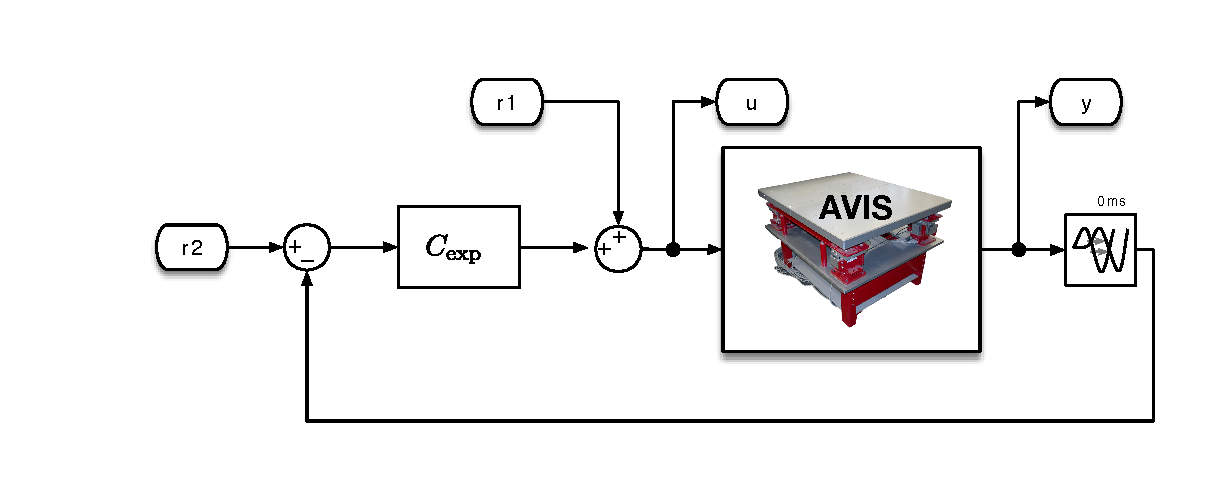
\includegraphics[width=\figurewidth]{\thisDir/figs/simulink-setup.pdf}
  \caption{Simulink model used during the AVIS measurements. All signals are six-dimensional real values.}
  \label{fig:avis:simulink:setup}
\end{figure}

In the top-level model (\figref{fig:avis:simulink:setup}), all signals are six-dimensional and each element corresponds to a mechanical degree-of-freedom of the \gls{AVIS}, i.e. 
\begin{enumerate}
  \item $v_x$: the velocity in $x$ direction (horizontal),
  \item $v_y$: the velocity in $y$ direction (horizontal),
  \item $v_z$: the velocity in $z$ direction (vertical),
  \item $\phi_x$: the angular velocity around the $x$ axis,
  \item $\phi_y$: the angular velocity around the $y$ axis,
  \item $\phi_z$: the angular velocity around the $z$ axis.
\end{enumerate}
The coordinate frame and axes are indicated in \figref{fig:avis:withAxes}.

\begin{figure}
  \centering
  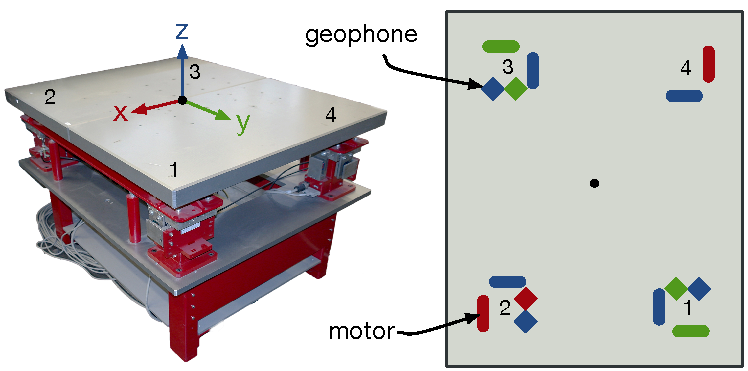
\includegraphics{\thisDir/figs/avis-with-axes.pdf}
  \caption{\glsentrytext{AVIS} with $(x,y,z)$ coordinate frame indicated and bird's eye view of the approximate locations of the actuators and sensors at each of the four corners. For each of the actuators and sensors, the color indicates the principal direction.}
  \label{fig:avis:withAxes}
\end{figure}

In the main text, we have simplified this system to consider only $v_z$, the vertical translation (i.e. the third signal).
For the other directions, the applied signals (\code{r1} and \code{r2}) were set to $0$.
However, inside the feedback loop, all directions are controlled by the experimental controller $\experimental\Controller$.

Specifically, $\experimental\Controller$ is a $6\times6$ transfer function matrix that is implemented as a discrete state-space model.
This controller was constructed by~\citet{Rademakers2005MSc}
 and is given by the state-space matrices below
\begin{align}
  \experimental\Controller & \isdef 
  \begin{cases}
     x[n+1] &= A x[n] + B u_c\\
       y_c    &= C x + D u_c 
  \end{cases}\\
  A       &\approx 828.8 \cdot 10^{-3} \cdot \Identity{6} \\
  B = C &\approx \AvisMatrixDiagonal{93.83}{39.57} \cdot 10^{-3}\\
  D       &= \AvisMatrixDiagonal{4.982}{0.886} \cdot 10^{-3}
\end{align}
with $\Identity{n}$ the $n\times n$ identify matrix.
It can be seen that the controller is diagonal, i.e. the directions are decoupled, and that the dynamics are common among the translational directions and the rotational directions respectively, such that
\begin{equation}
  \experimental\Controller = 
  \AvisMatrixDiagonal{\experimental\Controller_{\mathrm{tran}}}{\experimental\Controller_{\mathrm{rot}}}
\end{equation}
with
\begin{align}
\experimental\Controller_{\mathrm{tran}} &  \approx 
   \frac{4.9821 z + 4.6787}{ z - 0.8282} \cdot 10^{-3} \\
  \experimental\Controller_{\mathrm{rot}} & \approx 
    \frac{0.88595 z + 0.83201}{ z - 0.8282} \cdot 10^{-3}
\end{align}
 as visualized in \figref{fig:avis:bodeplots:controllerAndSensor}.

\begin{figure}[p]
\setlength\figurewidth{0.75\columnwidth}
\setlength\figureheight{0.68\figurewidth}
% This file was created by matlab2tikz.
%
%The latest updates can be retrieved from
%  http://www.mathworks.com/matlabcentral/fileexchange/22022-matlab2tikz-matlab2tikz
%where you can also make suggestions and rate matlab2tikz.
%
\begin{tikzpicture}


\pgfplotsset{amplitudePlot/.append style={%
  height=0.5\figureheight,
  ylabel={Amplitude \axisunit{dB}}}}
\pgfplotsset{phasePlot/.append style={%
  height=0.5\figureheight,
  ylabel={Phase \axisunit{rad}},
  ytick={-3.1416,-1.5708,0,1.5708,3.1416},
  yticklabels={{$-\pi$},$-\pi/2$,$0$,$\pi/2$,$\pi$},
  ymin=-3.142,
  ymax=3.142
  }}
\pgfplotsset{controllerAmpl/.append style={ymin=-80,ymax=-20}}
\pgfplotsset{filterAmpl/.append style={ymin=-20,ymax=20, yticklabel pos=right, ylabel near ticks, ytick={-20,0,20}}}
\pgfplotsset{noXTicks/.append style={xticklabels={}}}
\pgfplotsset{noYTicks/.append style={yticklabels={}}}
\pgfplotsset{noXLabel/.append style={xlabel={}, noXTicks}}
\pgfplotsset{noYLabel/.append style={ylabel={}, noYTicks}}


\begin{groupplot}[%
group style={%
  group name=derivs,
  group size=3 by 2,
  horizontal sep=0.5em,
  vertical sep=1em},
xlabel={Frequency $\omega \axisunit{Hz}$},
scale only axis,
xmode=log,
xmin=0.00016,
xmax=500,
xtick={0.01, 1, 100},
xminorticks=true,
grid=major,
width=0.33\figurewidth]


% ================================================
\nextgroupplot[amplitudePlot, controllerAmpl, noXLabel, title={$\experimental\Controller_{\mathrm{tran}}$}]
\addplot[myDerivs] table[] {\thisDir/data/avis-setup/Ctran-mag.tsv};

% ================================================
\nextgroupplot[amplitudePlot, controllerAmpl, noYLabel, noXLabel, title={$\experimental\Controller_{\mathrm{rot}}$}]
\addplot[myDerivs] table[] {\thisDir/data/avis-setup/Crot-mag.tsv};

% ================================================
\nextgroupplot[amplitudePlot, filterAmpl, noXLabel, title={$F_{\phantom{rot}}$}]
\addplot[myDerivs] table[] {\thisDir/data/avis-setup/sensFilter-mag.tsv};

% ================================================
% ================================================

% ================================================
\nextgroupplot[phasePlot]
\addplot[myDerivs] table[] {\thisDir/data/avis-setup/Ctran-phase.tsv};

% ================================================
\nextgroupplot[phasePlot, noYLabel, noYTicks]
\addplot[myDerivs] table[] {\thisDir/data/avis-setup/Crot-phase.tsv};

% ================================================
\nextgroupplot[phasePlot, noYLabel, noYTicks]
\addplot[myDerivs] table[] {\thisDir/data/avis-setup/sensFilter-phase.tsv};

\end{groupplot}

\end{tikzpicture}%

\caption{Bode plots of the elements of $\experimental\Controller$ and sensor filter $F$ present in the set-up.}
\label{fig:avis:bodeplots:controllerAndSensor}
\end{figure}

For multisine excitations the \code{RepeatingSequence} block was used to load the \code{r2} signal from \MATLAB, for noise excitations, the \code{RandomNumber} block of \Simulink was used instead.
The signals \code{r2}, \code{u} and \code{y} are returned from \Simulink to \MATLAB where further processing of the data is carried out.
This allows to compute the transfer function from \code{r2} to \code{u} and \code{y} respectively, or, the transfer function of the \gls{AVIS} block in the \Simulink model.

\begin{figure}[p]
\setlength\figurewidth{\columnwidth}
  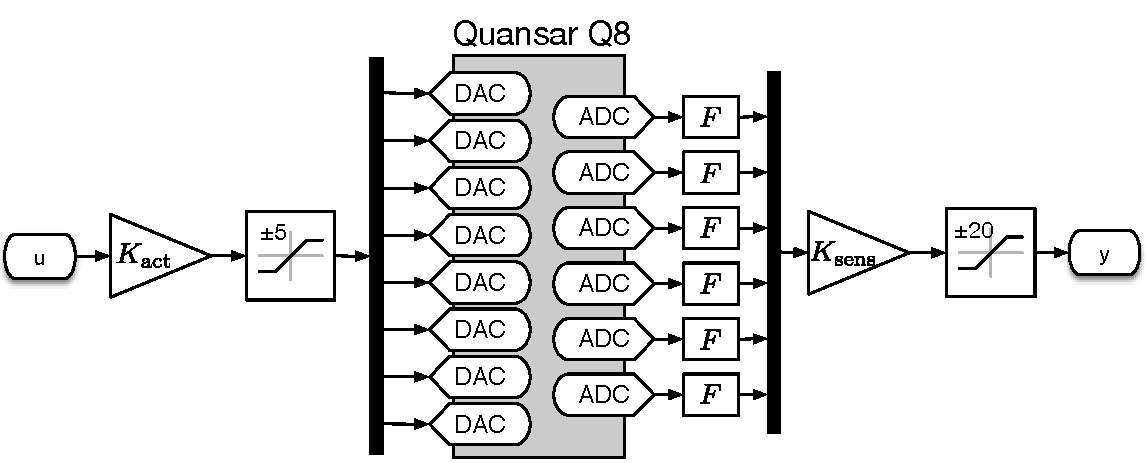
\includegraphics[width=\figurewidth]{\thisDir/figs/simulink-avis.pdf}
  \caption{Simulink model of the AVIS sub-block.}
  \label{fig:avis:simulink:avis}
\end{figure}

The \gls{AVIS} block (\figref{fig:avis:simulink:avis}), conceptually, contains:
\begin{itemize}
  \item static transformations $(K_{\mathrm{act}}, K_{\mathrm{sens}})$, as derived from first principles in~\citep{Rademakers2005MSc}, which translates the sensor and actuator signals to physical velocities at the center of the payload,
  \item logic to communicate with the Quanser Q8 \gls{DAQ} board which is physically connected to the \gls{AVIS}, and
  \item signal conditioning.
\end{itemize}

In \citet[Appendix A.4]{Rademakers2005MSc}, linear static relationships are derived to link the velocities at the center of the payload to the corresponding actuator voltages.
This yields the matrix:
\begin{align}
  K_{\mathrm{act}}    & \approx \begin{bmatrix}
     \deemph{0} &   -0.5 &      \deemph{0} &      \deemph{0} &      \deemph{0} & -0.6485\\
0.0974 & 0.1233 &  -0.25 & -0.6667 & 0.5263 &      \deemph{0}\\
  -0.5 &      \deemph{0} &      \deemph{0} &      \deemph{0} &      \deemph{0} & -0.5119\\
0.0974 & -0.1233 & -0.255 & 0.6667 & 0.5263 &      \deemph{0}\\
     \deemph{0} &    0.5 &      \deemph{0} &      \deemph{0} &      \deemph{0} & -0.6485\\
-0.0974 & -0.1233 &  -0.25 & 0.6667 & -0.5263 &      \deemph{0}\\
   0.5 &      \deemph{0} &      \deemph{0} &      \deemph{0} &      \deemph{0} & -0.5119\\
-0.0974 & 0.1233 &  -0.25 & -0.6667 & -0.5263 &      \deemph{0}\\
\end{bmatrix}
\\
\end{align}
Note that $K_{\mathrm{act}} \in \RR^{8\times6}$ and hence produces signals for the $8$ actuators on the \gls{AVIS}.
These signals are limited to the range $\pm 5\unit{V}$ before they are sent to the \glspl{DAC} on the Q8 \gls{DAQ} board to avoid overdriving the \glspl{DAC}.

The $6$ velocity signals that are digitized by the Q8 \gls{DAQ} are each filtered to transform the voltage induced in the coils of the geophones on the \gls{AVIS} into a velocity using a filter $F$ with transfer function
\begin{equation}
  F(s) \approx \frac{6.51 s^2 + 122 s + 11.3}{6.4 s^2 - 16.6 s - 2.2}

\end{equation}
which is shown in \figref{fig:avis:bodeplots:controllerAndSensor}.
More information regarding this design is given in \citep[Appendix A.3]{Rademakers2005MSc}.
This filter is discretized automatically by \Simulink for the actual implementation.
These velocities are then linked by a linear transformation to the (angular) velocities

The output \code{y} is clipped to $\pm 20$ for easier detection of errors.
However, during normal operation and all the measurements, the signal levels were well within the linear region of this saturation block.

\begin{remark}
It should be noted that while the benchmark paper by \citet{Voorhoeve2015SYSID} deals with the same physical \gls{AVIS}, the experimental data of the benchmark is fundamentally different from the data presented here.
\Citet{Voorhoeve2015SYSID} only consider the `physical' \gls{AVIS} with $8$ inputs and $6$ outputs as indicated by the \code{QuanserQ8} block in \figref{fig:avis:simulink:avis} as the system under test.
The measurements of the benchmark data were carried out in open-loop.
Hence, the experimental controller ($\experimental\Controller_{\mathrm{benchmark}} = 0$),the saturations, the filter $F$ and the static matrices $K$ are different.
Moreover, the sample rate of the benchmark data is much higher ($\fs  = 20 \unit{kHz}$) compared to the data in this work ($\fs = 1\unit{kHz}$) thanks to an upgrade of the real-time computer responsible for acquiring the signals.
\end{remark}


\end{subappendices}

   \chapter{Initialization of Parametric Estimators}
\label{sec:initvals}
\myEpigraph{Everything starts somewhere, though many physicists disagree. But people have always been dimly aware of the problem with the start of things. They wonder how the snowplough driver gets to work, or how the makers of dictionaries look up the spelling of words.}{Terry Pratchett}{Hogfather}
\gdef\thisDir{ch05-initvals}
\tikzsetfigurename{ch05fig}
\researchBasedOn{Geerardyn2015TIM}

\section{Introduction}
\label{sec:initial-values:introd}
The task of interpreting measurement data from dynamic systems often involves the estimation of a transfer function (TF). 
Typical measurement techniques and identification strategies of  \glspl{TF} or \glspl{FRF} are presented in~\citep{Schoukens1998,Schoukens2006LPM,Guillaume1996,Broersen1995,Pintelon2010LPM1,Antoni2007FRF}.
Application of these methods to real devices and systems is well-represented in the literature, e.g. \citep{Lim2010,Robinson1990,Behjat2010}.

Parametric identification of \gls{LTI} systems from either input/output data or non-parametric frequency response data, has been well developed as evidenced by published literature~\citep{Pintelon2012,Ljung1999,Schoukens1999,Pintelon1998}.
Many of such parametric identification algorithms, however, require solving non-linear or non-convex optimization problems.
This often involves an iterative algorithm to produce the optimal model.
 The resulting model, however, depends on which initial estimates are used to start up the optimization process: typically one can end up in local minima, leading to models of sub-optimal quality.
 Hence, good initial estimates are essential to obtain a high quality model estimate.
 In this chapter, the \gls{MLE} is used as a proxy for any parametric transfer function estimator, since the \gls{MLE} is commonly used and has desirable properties such as efficiency and consistency.
 Numerous other parametric identification techniques are devoted to the development of parametric plants $G(q^{-1},\theta)$ and parametric noise models  $H(q^{-1},\theta)$, where  $\theta$ is the model parameters vector  \citep{Ljung1999,Soderstrom1989,Pintelon2012}.
 Since the initial value generation method are not specifically tailored towards the \gls{MLE}, other parametric identification frameworks are likely to benefit from these improved starting values as well.
 Hence, the presented approach is orthogonal to initialization schemes such as the work of~\citet{vanHerpen2014} that focuses on improving the optimization algorithm, rather than the starting values.

 In the perspective of developing identification tools that require minimal user interaction, it is important that good initial estimates are produced for a wide variety of systems and experimental settings; i.e. to increase the probability of the optimization algorithm to produce good estimates, or preferably even the global optimum.
 However, when noisy input-output measurements are to be processed, the presence of noise obstructs a clear view of the actual system behavior, especially for poor \glspl{SNR}.
 Such problems can be mitigated using non-parametric techniques: the presence of noise is typically reduced by averaging multiple measurements or by using more advanced smoothing techniques.

The main aim and contribution of this chapter is to demonstrate that smoothing a measured \gls{FRF} non-parametrically, helps to avoid local optima during the parametric estimation of the \gls{MLE} of a transfer function, using classical (deterministic) optimization algorithms.
Hence, such techniques make it possible to increase the ``success rate'' (i.e. the probability that a good model, or even the global optimum, is obtained) of such a system identification step considerably.

In particular, two different smoothing techniques --- the time-truncated \gls{LPM}~\citep{Lumori2014TIM} and the \gls{RFIR}~\citep{Pillonetto2010,Chen2012} --- are tested for different \glspl{SNR} and different measurement record lengths of the input/output data of a few \gls{SISO} \gls{LTI} systems.
These are compared with the existing initialization schemes, namely: (i) the \gls{GTLS}, and (ii) the \gls{BTLS}.

\paragraph{Outline}
The rest of the chapter is structured as follows. 
\secref{sec:initial-values:ProbForm} covers the problem formulation. 
\secref{sec:initial-values:MethodEg} presents the methodology for obtaining the initial estimates, and their influence on the success rate of the \gls{MLE}. 
This is followed by \secref{sec:initial-values:Demo} and \secref{sec:initial-values:ExpMeas}, which are demonstrations of the improved initial estimates on simulation and experimental data, respectively.
In \secref{sec:initial-values:Generality} the generality of the results is investigated briefly.
The computational effort and recommendations for practical implementations are given in \secref{sec:initvals:computation}.
Ultimately, concluding remarks are presented in \secref{sec:initial-values:Conclusion}.

\section{Problem Formulation}
\label{sec:initial-values:ProbForm}

In this section, the assumptions on the system and the noise are presented, together with the associated MLE (formulated in the frequency domain), which turns out to be a non-convex function in the parameters, requiring initial estimates. The procedure for obtaining the initial estimates is elaborated in the subsequent sections.

\subsection{System Framework and Model}
\figref{fig:oesetup} depicts a schematic of the output error framework for  a generalized (single- or multiple-order) resonating, dynamic \gls{LTI} discrete-time \gls{SISO} system, subjected to a known white random noise input. 
The full model of the system is
\begin{equation}
y(t)=\true{G}(q^{-1})u_0(t)+H_0(q^{-1})e(t)
\label{eq:initial-values:OE:TD}
\end{equation}
where $\true{G}(q^{-1})$ represents the dynamics of the system to be estimated, $u_0(t)$ is the input signal, $v(t)= H_0(q^{-1})e(t)$ is the noise source at the output, $H_0(q^{-1})$ is the noise dynamics, 
$e(t)$ is white Gaussian noise, and $q^{-m}$ is the backwards shift operator ($q^{-m}x(t)$ = $x(t-mT_{\mathrm{s}})$  with $m$ a positive integer and $T_{\mathrm{s}}$ the sampling time).
We only treat the discrete-time case (i.e. $t = n \cdot T_{\mathrm{s}}$ for integer values of $n$) theoretically in this chapter.
However, the generalization to continuous time is straightforward~\citep[Chapter 6]{Pintelon2012} and has been demonstrated in Section~\ref{sec:initial-values:ExpMeas}.

\begin{figure}[tbh]
\centering
\tikzstyle{block}     = [draw,rectangle,minimum height=2em,minimum width=1.5em,inner sep=2mm]
\tikzstyle{sum}       = [draw,circle,inner sep=0mm,minimum size=2mm]
\tikzstyle{input} = []
\tikzstyle{output} = []
\tikzstyle{pinstyle} = [pin edge={<-,black},color=black]

\begin{tikzpicture}[auto, node distance=2cm,>=latex]

    \node [near start] (input) {$\true{u}(t)$};
    \node [block, right of=input] (system) {$\true{G}(q^{-1})$};
    \node [sum, right of=system,
           node distance=2.2cm] (sum) {\footnotesize$+$};
    \node [right of=sum, node distance=1.3cm] (output) {$y(t)$};

    \node [above of=sum, node distance=1.3cm] (noise) {$v(t)$};

    \draw [->] (input)  --   (system);
    \draw [->] (system) -- node[name=y0] {$\true{y}(t)$} (sum);
    \draw [->] (sum)    --    (output);

    \draw [->] (noise) -- (sum);

\end{tikzpicture}

\caption[Output-error set-up.]{SISO LTI discrete-time system in an output error setup.}
\label{fig:oesetup}
\end{figure}

In this chapter we assume that the output signal is disturbed by random noise, resulting in noisy error-prone data.
For the simulations, white noise is used ($\true{H} = 1$ and $e(t) = v(t)$).
It is also possible to apply the estimation procedure in this chapter to a system that is disturbed by colored noise, as will be demonstrated in \secref{sec:initial-values:ExpMeas}. 

With reference to equation \eqref{eq:initial-values:OE:TD}, the relation between the noiseless input and the output signals ($v(t)= 0$) is assumed to be of the form
\begin{equation}
    A(q^{-1}) y_0(t) = B(q^{-1}) u_0(t) \quad \forall t \in n \Ts{}  \text{ with }  n \in \IntegerNumbers
\label{ABpolys}
\end{equation}
where $A$ and $B$ are polynomials in $q^{-1}$. 
Thus, it follows from equation \eqref{eq:initial-values:OE:TD} that
\begin{equation}
    \true{G}(q^{-1})= \frac{B(q^{-1})}{A(q^{-1})}
    \text{.}
\end{equation}

From~\citet[Section 6.3.2.]{Pintelon2012}, in the frequency domain, and for the \glspl{DFT} of the windowed signals, equation \eqref{ABpolys} is of the form
\begin{align}
A(e^{-j\omega_k})\true{Y}(k) = B(e^{-j\omega_k})\true{U}(k) + I(e^{-j\omega_k})
\label{DFTspectra}
\end{align}
with $q^{-1}$ sampled in  $q_k^{-1} = e^{-j\omega_k}$, where $\omega_k = \frac{2\pi k}{N}$ are the \gls{DFT} frequencies, and $I$ is a polynomial of order $\max(N_a,N_b) - 1$, which depends on the difference between the initial and end conditions of the filters $\true{G}$ and $\true{H}$ during the measurement record.

\begin{remark}
The knowledge of the true model orders makes the analysis of the smoothers easier to carry out as we thus avoid extra calculation time required to perform model selection.
However, these smoothers can be used in conjunction with model order selection procedures.
\end{remark}

\begin{assumption}
It is assumed that the orders of the polynomials $A$, $B$ and $I$ are known.
\end{assumption}


\subsection{Parametric Identification Algorithm}\label{sec:initial-values:paramIdentAlgo}

The maximum likelihood estimate of the parameter vector $\theta$  containing the coefficients of the $A$, $B$ and $I$  polynomials is obtained by solving the optimization problem
\begin{equation}
  \hat{\theta} = \arg\min_\theta V(\theta) \text{.}
\end{equation}
Since the noise $v(t)$ is assumed to be Gaussian, $V(\theta)$ accords to the weighted least squares cost function~\citep[Section 9.11]{Pintelon2012}:
\begin{equation}\label{eq:MLEcf}
V(\theta) = \sum_{k=1}^{N/2-1}\frac{|\varepsilon(k,\theta)|^2}{\sigma_\varepsilon^2(k,\theta)}
\end{equation}
for $N$ measurements and when $\varepsilon$ denotes the error in equation \eqref{DFTspectra},  \emph{viz}.:
\begin{align}
\varepsilon(k,\theta) = A(k,\theta)Y(k) - B(k,\theta)U(k) - I(k,\theta)\text{.}
\end{align}
The variance of the error is of the form:
\begin{equation}\label{eq:sigmaEps}
\begin{split}
\sigma_\varepsilon^2(k,\theta) 
  &=  |A(k,\theta)|^2\sigma_Y^2(k) 
   +  |B(k,\theta)|^2\sigma_U^2(k)
  - 2\RealPart \left( A(k,\theta) \overline{B(k,\theta)} \sigma_{YU}(k) \right)
\end{split}
\end{equation}
where $\sigma_Y^2$ is independent of $k$ for white noise, and the input error variance is assumed to be zero, i.e. $\sigma^2_U=0$, and similarly, the covariance $\sigma_{YU} = 0$.
Here, $\overline{B}$ denotes the complex conjugate of $B$.

Consequently, $V(\theta)$ is a non-quadratic function of $\theta$ which, in general, results in a non-convex optimization problem. 
The Levenberg-Marquardt algorithm~\citep{Marquardt1963}, is used to solve this optimization problem deterministically and is shown in~\algoref{alg:initvals:levenberg-marquardt}.
Such an approach requires good initial estimates of $\theta$ to avoid inherent local optima, which is the focus of this chapter.

\begin{algorithm}
\caption{Levenberg-Marquardt~\citep{Marquardt1963},~\citep[Sec. 9.L.4]{Pintelon2012}}
\label{alg:initvals:levenberg-marquardt}
\begin{algorithmic}[1]
  \Require Cost function \eqref{eq:MLEcf} is rewritten as $V(\theta) = \InnerProductSelf{\epsilon(\theta)}$. 
\Function{LevenbergMarquardt}{$\epsilon(\theta),  \theta^{\mathrm{init}}$}
   \State $\atIter[0]{\theta} \gets \theta^{\mathrm{init}}$
   \Comment{$\atIter[i]{X}$ denotes $X$ at iteration $i$.}
   \For{$i$ \textbf{in} $1 \to \infty$}
      \State $U \, \Sigma \, W^{\TT} \gets \code{svd}\left( \frac{\partial \epsilon(\atIter[i-1]{\theta})}{\partial \theta}\right)$ 
        \Comment{Singular value decomposition of Jacobian}
      % \State $
      %                  \text{Denote }\Sigma \equiv 
      %                  \left[ \begin{matrix} 
      %                  \sigma_1         & \deemph{0} & \deemph{\cdots} &           & \deemph{0}      \\
      %                  \deemph{0}      & \sigma_2    &                   &           &                   \\
      %                  \deemph{\vdots} &              & \ddots            &           & \deemph{\vdots} \\
      %                                    &              &                   & \sigma_n &                   \\
      %                   \deemph{0}      &              & \deemph{\cdots} &           & \deemph{0}      
      %                   \end{matrix}\right]
      %                $
      % \State \textbf{if} $i=1$ \textbf{ then} $\lambda \gets \max(\sigma) / 100$
      \If{$\lambda$ is undefined}
        \State $\lambda \gets \max(\Set{\Sigma_{11}, \ldots, \Sigma_{nn}})/100$
      \EndIf
      \State $\Sigma_{kk} \gets \frac{\Sigma_{kk}}{(\Sigma_{kk}^2 + \lambda^2)} \quad \forall k \in \Set{1, \ldots, n}$
      \State $\delta\theta \gets - W  \Sigma^{\TT}  U^{\TT} \epsilon(\atIter[i-1]{\theta})$
      \State $\atIter[i]{\theta} \gets \frac{(\atIter[i-1]{\theta} + \delta\theta) }{ \norm[2]{\atIter[i-1]{\theta} + \delta\theta} }$
      \If{$V(\atIter[i]{\theta}) > V(\atIter[i-1]{\theta})$} \Comment{Current step is a deterioration}
         \State $\atIter[i]{\theta} \gets \atIter[i-1]{\theta}$ \Comment{Restart loop from previous estimate}
          \State $\lambda \gets 10 \lambda$ 
      \Else
          \State $\lambda \gets 0.4 \lambda$
      \EndIf
      \If {$\norm[2]{\delta\theta} < n_{\theta}  \cdot 10^{-6} \norm[2]{\atIter[i]{\theta}}$}
          \State \textbf{return} $\hat{\theta} \gets \atIter[i]{\theta}$
      \EndIf
   \EndFor
\EndFunction
\end{algorithmic}
\end{algorithm}

\begin{remark}
Alternatively, stochastic optimization algorithms~\citep{Spall2012,Press2007} are less likely to get stuck in local optima since such algorithms use randomization either to select initial values or to iterate towards the optimum (or both).
However, due to this random influence, their results are not always exactly reproducible and can incur a huge computational cost compared to `classical' deterministic schemes where only a single or a few initial estimates are used to start the expensive iterative optimization procedure.
Stochastic optimization is not discussed in the remainder of this chapter.
\end{remark}

\section{Methodology}\label{sec:initial-values:MethodEg}
In this section, the considered methods for obtaining the initial estimates of $\theta$ are briefly explained. Then their influence on the success rate of the maximum likelihood estimator is described.
%}

\subsection{Initial Estimates Procedure}\label{sec:init:procedures}
\begin{figure}[p]
  \centering
  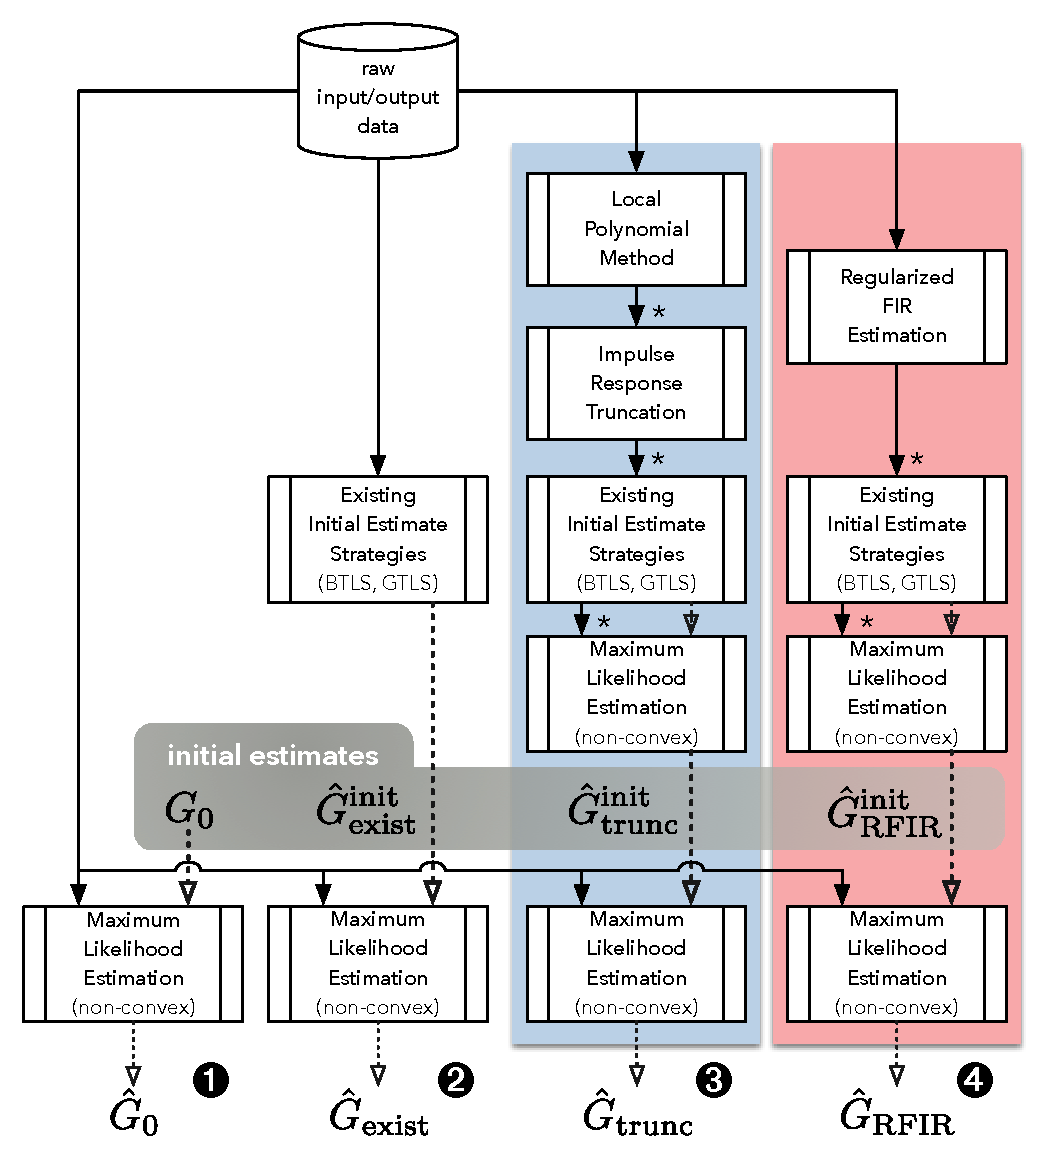
\includegraphics[width=\columnwidth]{\thisDir/figs/flowgraph}
  \caption[Flow chart of different initialization procedures.]{Flow chart depicting the different estimation procedures, from left to right: \circledNum{1} an approach using the true model as initial estimate; \circledNum{2} an existing approach using \gls{BTLS} and \gls{GTLS} starting values, and the novel initialization strategies outlined in this chapter (\circledNum{3}, \circledNum{4}) that make use of smoothers to generate improved starting values for the non-convex optimization problem.
  The flow of non-parametric data is depicted by full arrows, with the \gls{FRF} data marked by asterisks. Parametric models are indicated by dashed, unfilled arrows.} 
  \label{fig:flowgraph}
\end{figure}

The ultimate aim is to find initial estimates that are good enough to steer clear of the local optima during the \gls{MLE} optimization process in the parametric identification of each system. 
The requisite procedures for the estimators are as follows, from left to right of the flowchart in \figref{fig:flowgraph}:

\begin{enumerate}
\item \emph{Using the true model ($\true{G}$) as initial estimate}

The estimates from this procedure are for comparison purposes with those from the other procedures. They will be crucial to the computation of the global optimum of the \gls{MLE}.

\item \emph{Quadratic approximations of the \gls{MLE}}

The \gls{GTLS} and the \gls{BTLS} have been presented in \citep{Pintelon1998}. 
These are modifications of equation \eqref{eq:MLEcf}, which still take into account the noise information while retaining the quadratic nature w.r.t. $\theta$. 
These estimators preserve consistency, such that the estimates converge asymptotically to the true parameters for $N\to\infty$. 
Their finite sample behavior, however, is suitable for improvement by the \gls{FRF} smoothing tools as described below.

\item \emph{Local polynomial method (LPM) with truncation}
\disclaimer{The time-truncated \gls{LPM} has been explained in \secref{sec:nonparametric:truncation} in more detail. The pertinent details are repeated here to aid readability.}
A good estimate of the \gls{FRF} of the chosen system can be obtained via the truncated \gls{LPM}, which is summarized as follows~\citep{Lumori2014TIM} and \secref{sec:nonparametric:truncation} of this thesis.
Here, we repeat the main points briefly.
The \gls{LPM} is first applied to estimate the \gls{FRF} from a full input/output data record of the \gls{SISO} system.
The smooth characteristics of both the exact \gls{FRF} $\true{G}$ and the transient term $T$ allow for application of the \gls{LPM}, leading to a smooth \gls{FRF} estimate with the transient and noise suppressed.

  With reference to a detailed exposition in~\citep{Lumori2014TIM} and \chapref{sec:nonparametric}, the \gls{LPM} utilizes local polynomials to approximate the transfer function and transient contribution (in least squares sense) and, thus, smooth $\true{G}$ and $T$ around a central frequency $\omega_{k}$ in a local frequency band $r\in\mathbb{W}_n$.
  In this chapter, we limit the notations to quadratic polynomials in a window with half-width $N_W=3$, such that
\begin{subequations}\label{lpmImplQuadG}
\begin{align}
\true{G}(\omega_{k+r})&\approx \hat G_k + g_{1,k} r + g_{2,k}r^2
\\
T(\omega_{k+r})&\approx T(\omega_k)+t_{1,k}r + t_{2,k}r^2
\label{lpmImplQuadT}
\end{align}
\end{subequations}
where, in general,$r \in \LocalShifts[]$ with $\LocalShifts[] = \{-N_W,-N_W+1,\dots,N_W\}$ and $N_W$ is a tunable parameter. 

  The \gls{LPM} estimate of the \gls{FRF} at frequency index $k$ is the first estimated local parameter, \emph{viz}:
\begin{equation}
\hat{G}_{\LPM}(\omega_k) = \hat{G}_k
\text{.}
\end{equation}
This procedure is repeated for all $k$ in the frequency band of interest.

\emph{Impulse response truncation}. 
The estimate is smoothed further by truncating its impulse response function $g_{\LPM}(t) = \IDFT \left( \hat{G}_{\LPM}(\omega_k)) \right)$ as originally presented in~\citep{Lumori2014TIM} and \secref{sec:nonparametric:truncation}.

The impulse response is truncated after the time $\truncTime$ where the signal becomes indistinguishable from the noise, i.e.,
\begin{equation}
  g_{\trunc}(t) = 
  \begin{cases}
    g_{\LPM}(t) & t \leq \truncTime \\
    0                              & t \geq \truncTime
  \end{cases}
  \text{.}
\end{equation}

To this end, an estimate of the envelope of impulse response is determined by fitting an exponential function $g_{\mathrm{exp}}(t) = B e^{\beta t}$ to the peaks of $\abs{g_{\LPM}(t)}$ using a linear least-squares approach.
Then, $\truncTime$ is determined as the time instant where this envelope function sinks below the noise level $\sigma_g$ of the impulse response, i.e. 
\begin{equation}
  \truncTime = \min \Set{ t :  g_{\mathrm{exp}}(t) < \gamma \sigma_g  }
  = \beta^{-1} \ln \frac{\gamma \sigma_g}{B}
  \text{,}
\end{equation}
where $\gamma=1$ was used in this chapter for simplicity.
By changing $\gamma$, the user can fine-tune the bias/variance trade-off of the estimated \gls{FRF} $G_{\trunc}(\omega_k) = \DFT \left( g_{\trunc}(t)\right)$ further.
This can lead to a significant improvement over the classical LPM~\citep{Lumori2014TIM}.
 
\item \emph{\Glsfirst{RFIR}}

The \gls{RFIR} method is a special case of the \gls{RARX} method. 

The \gls{RFIR} estimator is formulated in the time domain. 
It estimates the impulse response of a discrete time system as the minimizer of the following regularized least squares objective function:
\begin{align}\label{eq:hRFIRdef}
\hat g_{\mathrm{RFIR}} &= \argmin_{g} \norm{y - g \ast u }^2 + \sigma^2 g^{\TT}P^{-1}g
\end{align}
where $g$ is the vectorized impulse response $g(t)$, with $t = 0,1,\cdots,n_h - 1$, assuming that the impulse response is $n_g$ samples long. 
Furthermore, $g\ast u$ is the convolution of $g$ with the input signal $u$, and $P\in \mathbb{R}^{n_g\times n_g}$ is the kernel matrix~\citep{Chen2012}. 
Note that \eqref{eq:hRFIRdef} is quadratic in $g$, such that $\hat g_{\mathrm{RFIR}}$ can be computed analytically in a single step.
The kernel matrix $P$ embodies prior knowledge on the system to be estimated. 
Here, the \gls{DCkernel}~\citep{Chen2012,Pillonetto2010} is used. 
Specifically, the element at $t_1,t_2$ of $P$ is given by
\begin{equation}
P(\alpha,\beta)_{t_1,t_2} = e^{-\alpha|t_1 - t_2|}e^{-\beta(t_1 + t_2)/2}
\end{equation}
 for $t_1,t_2 \in \left\{0,1,\cdots,n_h - 1\right\}$ which makes the estimated impulse response to be an exponentially decaying function of $t$ with decay rate $\beta^{-1}$, and correlation length $\alpha^{-1}$. 
 The latter \emph{hyperparameters} $\alpha$, $\beta$ and $\sigma$ are determined using Empirical Bayes~\citep{Carlin2000,Gelman2014}, i.e. as the maximizers of the \gls{LML} of the measured output signal~\citep{Chen2012}:
\begin{align}
\mathrm{LML}(y) = -y^{\TT}\Sigma(\alpha,\beta,\sigma)^{-1}y - \log |\Sigma(\alpha,\beta,\sigma)| \text{,}
\end{align}
where $\Sigma(\alpha,\beta, \sigma) = \sigma^2 \I + \phi^{\TT}P(\alpha,\beta)\phi$ and $\phi$ is a Toeplitz matrix constructed with $u$. 
This problem is solved using \mcode{fmincon} in \MATLAB.

An implementation of the \gls{RFIR} estimator is available as the \mcode{arx} function in the System Identification Toolbox since \MATLAB~2013b with $\mathtt{na} = 0$, $\mathtt{nb} = n_g$, $\mathtt{nk}=0$ and regularization enabled in \mcode{arxOptions}. 
The hyperparameters can be determined via \mcode{arxRegul}.
More information about the \gls{RFIR} estimator can be found in
~\citep{Pillonetto2010,Chen2012}. 
The \gls{DFT} of the obtained regularized estimate of the impulse response $\hat g_{\mathrm{RFIR}}$ of the system yields a smoothed estimate of the \gls{FRF}.
\end{enumerate}

\begin{remark} \label{rem:initvals:orders:RFIR}
In this chapter, all results are obtained using $n_g=200$ since this exceeds the length of most impulse responses used.
However, for general use, the model complexity $n_g$ might need to be increased.
One could use $n_g \approx N$ and rely on regularization to reduce the effective model complexity.
Unfortunately, this scales very poorly for long measurement records as explained in \secref{sec:initvals:computation}.
\end{remark}

\begin{remark}
The \gls{LRM} has also been tried to generate better initial values.
However, given the discussion in \chapref{sec:nonparametric}, it is clear that the \gls{LRM} performs poorly in low \gls{SNR} situations.
The same was apparent from the quick trial we ran on \gls{LRM} starting values.
As such, the use of \gls{LRM} over \gls{LPM} offers no advantage for generating initial estimates in the settings used in this chapter.
\end{remark}


\begin{remark}
Note that methods 3) and 4) result in a non-parametric estimate of the transfer function, represented as the \gls{FRF}. 
A corresponding parametric estimate is obtained as follows. 
A parametric estimator (\gls{GTLS}, \gls{BTLS}, and \gls{MLE}) is invoked, where the input spectrum is considered to be $1$ at all frequencies (Dirac in the time domain), and the output spectrum is set equal to the estimated \gls{FRF} $G_{\bullet}(\omega_k)$, with the transient term $I$ set to zero:
\begin{equation}
  U_{\mathrm{FRF}}(\omega_k) \isdef 1 
  \qquad \text{and} \qquad
  Y_{\mathrm{FRF}}(\omega_k)  \isdef G_{\bullet}(\omega_k)
  \text{.}
\end{equation}
It is important to note that invoking the \gls{GTLS}, \gls{BTLS} and \gls{MLE} on the \glspl{FRF} from methods 3) and 4) will yield a different result from applying the \gls{GTLS}, \gls{BTLS} and \gls{MLE} on the raw data. 
This is because the \glspl{FRF} from 3) and 4) have been smoothed and, thus, have a significantly reduced noise variance, but might be biased slightly.
\end{remark}

\subsection{Success Rates of the Initial Estimates}
The initial estimates described above are then fed to the \gls{MLE} together with the raw data to obtain the final estimates.

Formally, let $\model{\bullet}$ be the final parametric estimate of the system, where the subscript $\bullet$ denotes the methods (from left to right in Fig.~\ref{fig:flowgraph}) when an initial estimate $\model[init]{\bullet}$ is used, \emph{viz}:
\begin{itemize}
    \item $\model{\trueSymbol}$ via the true model $\true{G}$ as an initial estimate,
    \item $\model{exist}$ is obtained via \gls{GTLS} and \gls{BTLS},
    \item $\model{trunc}$ by the use of the \gls{LPM} with truncation as an initial estimate,
    \item $\model{RFIR}$, initialized by means of the \gls{RFIR} method. 
\end{itemize} 

A particular initial estimate is deemed \emph{successful} if the optimization of the \gls{MLE} cost with the raw input-output data inserted in equation~\eqref{eq:MLEcf}, approximately reaches the \emph{best local optimum} when iteration is initiated with the selected initial value/estimate.

\begin{conjecture}\label{conj1}
The true model $\true{G}$ as an initial estimate is the best possible initial estimate one can use for the nonlinear optimization algorithm (the leftmost path in \figref{fig:flowgraph}) and will allow the optimization to converge to the \emph{best local optimum}, i.e. $\model{\trueSymbol}$.
\end{conjecture}
\begin{remark}
The use of $\true{G}$ as an initial estimation not necessarily entails in converging to the global optimum since it is not guaranteed that $\true{G}$ lies within the attraction region of the global optimum.
\end{remark}

From this conjecture, use of the true system as an initial estimate would engender the best final estimate or hopefully even the global optimum.
Since the true system is not really known in practice, this chapter compares the capability of different possible initial estimates to emulate the result that would be obtained by using the true model as an initial estimate. 

The capability is quantified by defining the success rate of the initial estimate as the probability that the identification algorithm reaches the \emph{best local optimum} when the selected initial estimate is used. 
Note that probability in this context should be understood with respect to different realizations of the input signal and disturbing noise.

The success rate $\successRate_{\bullet}$ of an initialization scheme $\bullet$ is expressed mathematically as the probability function
\begin{equation}
\successRate_{\bullet} = 
  \Prob{  \model{\bullet}=\model{\trueSymbol}  }
\text{.}
\end{equation}
In practice, and since the iterative algorithm usually does not reach the local optimum precisely, the above definition is relaxed to the form
\begin{equation}\label{eq:successrateTol}
\successRate_{\bullet} \isdef \Prob{ \norm[2]{\model{\bullet} - \model{\trueSymbol}} < \absoluteTolerance}
\end{equation}
with $\absoluteTolerance$ a numerical tolerance that will be specified later on.

\begin{remark}
For an automated approach, it is better to define the success rate in terms of relative errors on the transfer function, i.e.
\begin{equation}
\successRate_{\bullet} = \Prob{ \norm[2]{\model{\bullet}-\model{\trueSymbol}} < \relativeTolerance  \norm[2]{\true{G}}}
\text{.}
\end{equation}
\end{remark}
\begin{remark}
In this chapter, the absolute criterion is used.
However, the results are equivalent for a relative criterion when the separation between successful and failed estimates is large since then observed success rate $\successRate$ is not sensitive towards the tolerance $\absoluteTolerance$ (or $\relativeTolerance$) when the tolerance is chosen with care.
Consequently, one can easily determine the equivalent relative tolerance from the absolute one using $\absoluteTolerance = \relativeTolerance \norm[2]{\true{G}}$.
\end{remark}

The $\mathcal{L}_2$ norm used in equation \eqref{eq:successrateTol} is defined~\citep{Skogestad2005} as
\begin{align}
\norm[2]{G(z)} &\isdef \sqrt{\frac{1}{2\pi}\int_0^{2\pi} |G(e^{-j\omega})|^2\ \mathrm{d}\omega}& \text{ for discrete time,}\\
\norm[2]{G(s)} &\isdef \sqrt{\frac{1}{2\pi}\int_{-\infty}^{+\infty} |G(j\omega)|^2\ \mathrm{d}\omega}& \text{ for continuous time}
\end{align}
 which, in practice, is computed by using the adaptive global quadrature algorithm provided by the \MATLAB function \code{integral}.
The success rate in equation \eqref{eq:successrateTol} is estimated via Monte Carlo simulations in \secref{sec:initial-values:CompuSR}.

\begin{remark}
The specific norm that is used in~\eqref{eq:successrateTol} can be adapted to suit the eventual purpose of the models the user wants to obtain.
E.g. in robust control, it often makes sense to rather have a $\Hinf$ norm as in \chapref{sec:hinf} than an $\mathcal{L}_2$ norm.
In this chapter, the $\mathcal{L}_2$ norm has been chosen since this is more closely related to the cost function~\eqref{eq:MLEcf}.
\end{remark}

\section{Demonstration}\label{sec:initial-values:Demo}

\subsection{The System Under Consideration}

Two systems are considered. 
The first, with a quality factor $Q = 6\unit{dB}$, has the transfer function
  \begin{equation}
     \true{G}(z)
    \approx 
    1.74 \cdot 10^{-3}
    \frac{ z^2 + 2 z + 1 }
         { z^2 - 1.93 z + 0.94}
    \text{ i.e. }
    \timeconst \approx 32 \unit{s}
    \text{ for } Q = 6 \unit{dB}
    \label{eq:systemundertest}
    \text{,}
  \end{equation}
where $\timeconst = (\damping \wn)^{-1}$ denotes the time constant of the system (with $\damping$ the damping and $\wn$ the frequency of the dominant pole).
The second system, with a quality factor $Q = 20\unit{dB}$, has the transfer function
  \begin{equation}
    \true{G}(z)
    \approx
    309 \cdot 10^{-6}
            \frac{z^2 + 2 z + 1}
                 {z^2 - 1.98 z + 0.989}
    \text{ i.e. }
    \timeconst \approx 180 \unit{s}
    \text{ for } Q = 20 \unit{dB}
    \label{eq:systundertest-20dB}
    \text{.}
  \end{equation}

Both systems are low-pass Chebyshev filters which have been generated using the \MATLAB command \mcode[mathescape]{cheby1(2, $\,Q$, 0.05)}.
Their transfer functions are shown in \figref{fig:exampleFRF}.
Their inputs are excited by zero mean white Gaussian noise with unit variance, and the outputs are disturbed by different realizations of white gaussian noise, as in \figref{fig:oesetup}, with a variance $\sigma_v^2$, such that a prescribed \gls{SNR} defined as
\begin{equation}
  \mathrm{SNR} 
    = \frac{\sigma_v}
           {\rms{y_0}}
    \approx \frac{\sigma_{v}}
                 {\left\| \true{G} \right\|_2 \rms{u_0}}
    =  \frac{\sigma_{v}}
            {\left\| \true{G} \right\|_2}
  \label{eq:SNR-definition}
  \text{.}
\end{equation}
is attained.
$\rms{x} = \sqrt{N^{-1} \sum_t x^2(t)}$ denotes the root-mean-squared value of $x$.

\subsection{Comparison of Successful and Failed Estimates}
 \figref{fig:exampleFRF} depicts the Bode plot of the actual system $\true{G}$, in black and different estimates $\model{exist}$ that may or may not approximate $\model{\trueSymbol}$ well, according to the distance defined by equation \eqref{eq:successrateTol}.
 The systems shown here are drawn randomly from the successes and failures observed in the Monte Carlo simulations, which are discussed later on in this chapter.
 
 It is clear from \figref{fig:exampleFRF} that the successful estimates virtually coincide with the true system. 
 This means that their distances from the true system, e.g. as given by $\norm[2]{\model{\bullet} - \true{G}}$, have small values. 
On the other hand, the `failed' estimates are inaccurate descriptions of the true system. 
It is apparent that their associated distances from the true system are larger by, at least, an order of magnitude than for the successful estimates.
 
 Estimation `failures' can be attributed to the optimization procedure getting stuck in local optima, resulting in very poor estimates of $\true{G}(\omega)$ over broad frequency ranges, as seen in \figref{fig:exampleFRF}. 
 Consequently, such estimates are approximations of $\true{G}$ that are practically worthless for most applications.
 %}


\begin{figure}
  \centering
  \setlength{\figurewidth}{0.8\columnwidth}
  \setlength{\figureheight}{0.6\figurewidth}
  % This file was created by matlab2tikz v0.4.7 (commit c12232582f3630004d70f33913f4929fdbccffdd) running on MATLAB 8.3.
% Copyright (c) 2008--2014, Nico Schlömer <nico.schloemer@gmail.com>
% All rights reserved.
% Minimal pgfplots version: 1.3
% 
% The latest updates can be retrieved from
%   http://www.mathworks.com/matlabcentral/fileexchange/22022-matlab2tikz
% where you can also make suggestions and rate matlab2tikz.
% 
\begin{tikzpicture}
\begin{axis}[%
width=0.45\figurewidth,
height=\figureheight,
scale only axis,
xmode=log,
grid=major,
xmin=0.01,
xmax=3.14159265358979,
extra y ticks={3,-6},
extra y tick labels={,$-6$},
xminorticks=true,
ymin=-50,
ymax=3,
name=sys6,
extra x ticks={3.14159265358979},
extra x tick labels={},
xlabel={Frequency \axisunit{rad/s}},
ylabel={Magnitude $\abs{G}$ \axisunit{dB}},
axis x line*=bottom,
axis y line*=left,
% title={$Q=6\unit{dB}$}
]
\addplot [bw]
  table[row sep=crcr]{%
0.0695459816004156  -50\\  
0.0695459816004156  -3.23569840496182\\
0.0773591356316033  -2.54077873681777\\
0.0849143289296425  -1.81553654790763\\
0.0921298190797872  -1.11816002831746\\
0.0989462912004401  -0.52871057336896\\
0.105324752461263   -0.134830655363943\\
0.111243778084011   -1.38867930760656e-05\\
0.117495440276076   -0.173635490071974\\
0.125069651547988   -0.831271091043913\\
0.134323265648525   -2.13034793822928\\
0.13946             -3\\
0.145737219128923   -50\\
0.0695459816004156  -50\\  
};
\label{leg:example-3db-bandwidth}

\addplot [badestimate,forget plot]
  table[row sep=crcr]{%
1e-20   21.9782591178994\\
7.94042926505012e-16    21.9782591178994\\
7.94042926505012e-12    21.9782591178994\\
7.94042926505012e-09    21.9782591161615\\
7.9404292650501e-07 21.9782417462284\\
7.9404292650501e-06 21.9765222945585\\
9.26585390428909e-06    21.9758942484213\\
1.08125197907783e-05    21.975039181067\\
1.26173567416011e-05    21.9738751024811\\
1.47234589369816e-05    21.9722904727581\\
1.7181113882136e-05 21.9701336043346\\
2.00490031244955e-05    21.9671983078602\\
2.33956033958875e-05    21.963204488287\\
2.73008216348132e-05    21.9577719844484\\
3.18579029283296e-05    21.9503854284653\\
3.71756569295581e-05    21.9403472793948\\
4.33810559110981e-05    21.9267154862839\\
5.06222664881953e-05    21.9082215451845\\
5.90721874002674e-05    21.8831642292584\\
6.89325778225682e-05    21.8492743829004\\
8.04388747798919e-05    21.8035475878087\\
9.38658146879394e-05    21.7420453980644\\
0.000109533993248164    21.659673915049\\
0.000127817520327028    21.5499628160924\\
0.000149152952595602    21.4048901640495\\
0.000174049717214562    21.2148273798551\\
0.00020310227545145 20.96870721497\\
0.000237004316661455    20.6545274194401\\
0.000276565321542103    20.2602659862579\\
0.000322729890143501    19.7751758060841\\
0.00037660029612997 19.1912564716577\\
0.000439462805822286    18.5045396465889\\
0.000512818390441587    17.7157860749401\\
0.000598418564872694    16.8303491062439\\
0.000698307208670757    15.8572541439332\\
0.000814869367873441    14.8078092642764\\
0.000950888202861922    13.6941565291411\\
0.00110961144201755 12.5280843349164\\
0.00129482892789138 11.3202456160321\\
0.0015109631074603  10.0797717647173\\
0.00176317462710996 8.81418792239232\\
0.00205748555364119 7.52951652364157\\
0.00240092316345372 6.23047439037121\\
0.00280168773316884 4.92069872018599\\
0.00326934833803568 3.60296464635629\\
0.00381507133320931 2.27937674080068\\
0.00445188697335947 0.95152902551602\\
0.00519500053669911 -0.379365331539551\\
0.00606215538215661 -1.71237041032276\\
0.00707405660842551 -3.04674475853281\\
0.0082548654306195  -4.38187412930866\\
0.0096327760787885  -5.71721477192484\\
0.0112406889929296  -7.05224270717482\\
0.0131169963884036  -8.38640469863179\\
0.0153064989487402  -9.71906671709192\\
0.017861475533752   -11.0494555692706\\
0.0208429314444294  -12.3765890516824\\
0.0243220550494984  -13.6991895872293\\
0.0283819175535854  -15.0155760006658\\
0.0331194564924369  -16.3235282665891\\
0.0386477903152057  -17.6201213939342\\
0.0450989193191982  -18.901528207293\\
0.0526268774274353  -20.1627983020324\\
0.0614114100641721  -21.3976339589931\\
0.0716622659451921  -22.5982050551367\\
0.0836242052581613  -23.7550734726481\\
0.0975828438136105  -24.8573267908223\\
0.113871472707625   -25.8930345956866\\
0.132879016329659   -26.850111345148\\
0.155059318729224   -27.7175710348094\\
0.180941980072474   -28.4869940154641\\
0.211145001931297   -29.1538580170766\\
0.2463895433371 -29.7183260592942\\
0.287517139930301   -30.1852166590516\\
0.335509797348016   -30.5631670408685\\
0.391513438620719   -30.8632791092607\\
0.456865265432541   -31.0976570760412\\
0.53312568655134    -31.2781751998317\\
0.62211557578523    -31.4156426808079\\
0.725959749075638   -31.5193710589221\\
0.847137698831549   -31.5970557456162\\
0.988542796891126   -31.6548573860542\\
1.15355137970273    -31.6975830643055\\
1.34610336527558    -31.7288939961242\\
1.51233425396771    -31.7466290418837\\
1.54633544891096    -31.749526700662\\
1.72816761362946    -31.7619219566801\\
1.76114911540292    -31.7637010545016\\
1.92951778716842    -31.7710038741036\\
1.96193742901404    -31.7721041118213\\
2.11343347193118    -31.776070626636\\
2.14586949308637    -31.7766732674033\\
2.27851870672999    -31.7781832185692\\
2.31156223924553    -31.7782970711387\\
2.42457990915855    -31.7776985209584\\
2.45876300546508    -31.7771474877182\\
2.55227834882998    -31.7743922531901\\
2.58803422991059    -31.7726910064887\\
2.66282840668659    -31.7673556920849\\
2.70047659961172    -31.7633627719598\\
2.75775716891478    -31.7546061086289\\
2.83872566473365    -31.7321514622295\\
2.9074042181334 -31.6917739787383\\
2.96539144508165    -31.6153742206904\\
3.01416632178943    -31.4587585452521\\
3.05506403042146    -31.0974062224372\\
3.08926806257214    -30.1062907999073\\
3.11781283849252    -26.6462929309358\\
3.14159265358979    -10.0779776823275\\
} ;
\label{leg:example-bad-estimate}

\addplot [badestimate,forget plot]
  table[row sep=crcr]{%
1e-20   -35.3344537468254\\
7.04369595145949e-18    -35.3344537468254\\
7.04369595145948e-13    -35.3344537468254\\
7.04369595145948e-09    -35.3344537468254\\
7.0436959514595e-06 -35.3344537449714\\
0.00070436959514595 -35.334435207486\\
0.0070436959514595  -35.3325992383233\\
0.00815208481511204 -35.3319694060822\\
0.00943488862817967 -35.3311255487005\\
0.0109195531505189  -35.3299948421723\\
0.0126378429789703  -35.3284796075159\\
0.0146265211551737  -35.3264487673018\\
0.0169281357157815  -35.3237263174325\\
0.0195919300134163  -35.3200757332342\\
0.022674896284814   -35.3151788073003\\
0.0262429950073827  -35.3086068070824\\
0.0303725661324743  -35.2997809418478\\
0.035151962388897   -35.2879177735729\\
0.0406834396014126  -35.2719531080571\\
0.0470853444678404  -35.2504345563657\\
0.0544946466025505  -35.2213674450857\\
0.0630698690197578  -35.1819893500765\\
0.0729944797547001  -35.1284318567372\\
0.084480817186891   -35.0551973184586\\
0.0977746330482662  -34.954318596653\\
0.113160350314492   -34.8139472998487\\
0.130967148472725   -34.6158483517765\\
0.15157600636095    -34.3306452654859\\
0.167973798548338   -34.0522714952775\\
0.191019153350675   -33.5642098134947\\
0.212854677989709   -32.9654650398389\\
0.233161323884123   -32.2445792321341\\
0.251751583065485   -31.3889880575135\\
0.2685466821325 -30.3842450458288\\
0.283551721057829   -29.2127724619399\\
0.296832197435992   -27.8518007651011\\
0.308493743898435   -26.2700018319872\\
0.318665759468638   -24.4221276371071\\
0.327488897589068   -22.2412033210837\\
0.335105986721603   -19.6321147074096\\
0.341655799062333   -16.5047970729923\\
0.347269061325413   -13.1163290481979\\
0.352066154705692   -11.4004279034841\\
0.356929514009032   -13.4758971636091\\
0.362793717037533   -17.4798432319057\\
0.369884699768814   -21.3621841648008\\
0.378487876083008   -24.8476494459257\\
0.388967354057539   -28.0456924838772\\
0.401792839371356   -31.0699680023249\\
0.417577939185591   -33.9909108685185\\
0.437135690190267   -36.8157234149246\\
0.440546371171951   -37.2375000684063\\
0.462370128016925   -39.5125738036581\\
0.485274988677512   -41.1971352046358\\
0.512720853680671   -42.4301247077615\\
0.545843448837804   -43.1088920433386\\
0.586142763763587   -43.2882760448732\\
0.635628916175986   -43.1384430405995\\
0.697038565240492   -42.8307266521388\\
0.774162169326941   -42.479386857925\\
0.872349172987367   -42.1447355594257\\
0.875482607753855   -42.1358800003179\\
1.01324766454265    -41.8282372213961\\
1.17269129118987    -41.6067650177977\\
1.35722480550033    -41.4477264007403\\
1.5707963267949 -41.3334898434371\\
1.80437115662468    -41.2553476887506\\
2.07267817941887    -41.1993355166117\\
2.38088201513671    -41.1607963452239\\
2.73491525422956    -41.1372400466171\\
3.14159265358979    -41.1287401183315\\
};

\addplot [badestimate,forget plot]
  table[row sep=crcr]{%
1e-20   -39.8838699689947\\
1.25494873076997e-17    -39.8838699689947\\
1.25494873076996e-12    -39.8838699689947\\
1.25494873076996e-08    -39.8838699689947\\
1.25494873076996e-05    -39.8838699680069\\
0.00125494873076996 -39.8838600908428\\
0.0125494873076996  -39.8828817993342\\
0.0144063638968654  -39.8825675871193\\
0.0165379920023961  -39.8821534007176\\
0.018985025050688   -39.8816073845632\\
0.0217941317254857  -39.8808874984915\\
0.0250188860114572  -39.8799382363591\\
0.0287207889324777  -39.8786862688014\\
0.0329704414707427  -39.877034643668\\
0.0378488910360824  -39.8748550428063\\
0.0434491771647171  -39.8719774021784\\
0.0498781059263073  -39.8681759248696\\
0.057258286879968   -39.8631501065943\\
0.0657304714271342  -39.8564987730381\\
0.0754562371572602  -39.8476841649482\\
0.0866210693809554  -39.8359815669781\\
0.0994378986201321  -39.8204074374188\\
0.114151161520544   -39.7996146674148\\
0.131041462634561   -39.7717359441043\\
0.150430925981551   -39.7341420992776\\
0.172689338448353   -39.6830551655825\\
0.198241202193937   -39.6129006853196\\
0.227573830558456   -39.5151645060334\\
0.261246641878127   -39.3762410984036\\
0.299739886201617   -39.1740143421048\\
0.338421981615247   -38.9097520847677\\
0.374899953514871   -38.5838250189013\\
0.40870356513184    -38.1880949784568\\
0.439570460742002   -37.7135029919643\\
0.467407372642824   -37.1499743012257\\
0.492249687495853   -36.4863173772628\\
0.51422417461499    -35.7100400055162\\
0.533517297971517   -34.8069586592356\\
0.550349885429558   -33.7604060112164\\
0.564957922716998   -32.5497209048177\\
0.577578716327419   -31.1474693493045\\
0.588441469960327   -29.5143160463484\\
0.59776131430865    -27.5891371731074\\
0.605735927582304   -25.2682111912805\\
0.612544023974351   -22.3548802942008\\
0.618345133722122   -18.4085544742421\\
0.623280232754262   -12.0924013333541\\
0.627472894099389   0.422692095266531\\
0.63169375850348    -12.5839927302902\\
0.636735394777761   -19.4922133519611\\
0.642765609359613   -24.1360391148694\\
0.64998989642391    -27.8707281139944\\
0.658661280689984   -31.1539477338544\\
0.669093279329902   -34.19450926611\\
0.681677183904867   -37.0919939036128\\
0.696905410116159   -39.8596089292055\\
0.715403497399034   -42.3905967088432\\
0.737974634236664   -44.4138608971605\\
0.747264731275601   -44.9483596821773\\
0.765662627830072   -45.6009411858482\\
0.775106105185704   -45.7741877329859\\
0.808393540553048   -45.8784096924836\\
0.848427177093714   -45.5750639363405\\
0.896900989597376   -45.1226715558277\\
0.956052583285154   -44.6575237071984\\
0.963344258331722   -44.6083508215325\\
1.02888227581772    -44.2350160840834\\
1.11947946164984    -43.8719678881029\\
1.23351857611959    -43.5694063665965\\
1.37902928040561    -43.3227372847522\\
1.5707963267949 -43.1234209841299\\
1.80437115662468    -42.9791508710005\\
2.07267817941887    -42.8814920524747\\
2.38088201513671    -42.8169012307825\\
2.73491525422956    -42.7784181321575\\
3.14159265358979    -42.764712611162\\
};

\addplot [badestimate,forget plot]
  table[row sep=crcr]{%
1e-20   -4.96388991523557\\
1.56474278893509e-18    -4.96388991523557\\
1.56474278893509e-13    -4.96388991523557\\
1.56474278893509e-09    -4.96388991523557\\
1.56474278893509e-06    -4.96388991697432\\
0.000156474278893509    -4.96390730275095\\
0.00156474278893509 -4.96562832290607\\
0.00182451269824627 -4.96625326663137\\
0.00212740816548347 -4.96710278971671\\
0.00248058865631137 -4.96825752654324\\
0.00289240221113011 -4.9698270033962\\
0.00337258276565312 -4.97195994021739\\
0.00393248022955158 -4.97485818290704\\
0.00458532876147795 -4.97879550957508\\
0.00534655958161914 -4.98414294939295\\
0.006234165715653   -4.99140274731951\\
0.00726912729147097 -5.00125370327461\\
0.00847590744130119 -5.0146112855857\\
0.00988303053074852 -5.03270658703049\\
0.011523756382209   -5.05718867649034\\
0.0134368664291119  -5.09025483888706\\
0.0156675803831237  -5.13481193664672\\
0.0182686250813515  -5.1946685862603\\
0.0213014807776237  -5.27475042589384\\
0.0248378343361296  -5.3813174784628\\
0.0289612736761976  -5.52214187841807\\
0.0337692635193859  -5.70657669800896\\
0.0393754491391365  -5.94541868752684\\
0.0459123425661525  -6.2504555884895\\
0.0535344547426785  -6.63361845095104\\
0.0624219476596412  -7.10575591599521\\
0.0727848928013203  -7.67520687487506\\
0.0848682365533569  -8.34650944139775\\
0.0989575899402285  -9.11964040499133\\
0.115385979542791   -9.99005139428043\\
0.134541719165667   -10.9494938896759\\
0.15687758831514    -11.9873564145323\\
0.182921534436991   -13.0921209463063\\
0.213289151880429   -14.2526117233791\\
0.248698232550323   -15.458874873231\\
0.289985732177924   -16.7026857062601\\
0.338127553237642   -17.9777752413006\\
0.394261612113818   -19.279897842694\\
0.459714735750443   -20.606854131313\\
0.536034023533312   -21.9585648204768\\
0.625023415697709   -23.3372800884326\\
0.728786332620085   -24.7480167142955\\
0.849775392848182   -26.1993521157451\\
0.990850385042444   -27.7047892860754\\
1.15534586409725    -29.285078306988\\
1.34714996919483    -30.9722151164288\\
1.48115733804343    -32.0880724268286\\
1.51233425396771    -32.342704065559\\
1.62508336131218    -33.2528807150039\\
1.70455653956782    -33.8877277474202\\
1.72816761362946    -34.0757452658069\\
1.84097037833582    -34.9729672231127\\
1.92413170852548    -35.635930204352\\
1.92951778716842    -35.6789751388916\\
2.04599501283918    -36.6145724292682\\
2.11343347193118    -37.1612816211174\\
2.23730281753708    -38.1758544067695\\
2.27851870672999    -38.5158969106663\\
2.42457990915855    -39.7204937457915\\
2.55227834882998    -40.7377814284692\\
2.66282840668659    -41.5170254021272\\
2.75775716891478    -41.9959580194214\\
2.83872566473365    -42.1012657335544\\
2.9074042181334 -41.745928209769\\
2.96539144508165    -40.8237882975128\\
3.01416632178943    -39.2003971050851\\
3.05506403042146    -36.6816219202571\\
3.08926806257214    -32.8855397054478\\
3.11781283849252    -26.7197281556705\\
3.14159265358979    -17.6564016527941\\
};

\addplot [badestimate,forget plot]
  table[row sep=crcr]{%
1e-20   -3.90062244934303\\
1.15704491996863e-18    -3.90062244934303\\
1.15704491996863e-13    -3.90062244934303\\
1.15704491996863e-09    -3.90062244934303\\
1.15704491996863e-06    -3.90062245107998\\
0.000115704491996863    -3.90063981881165\\
0.00115704491996863 -3.90235905233754\\
0.00135348643681851 -3.90299861072391\\
0.001583279527904   -3.9038736183256\\
0.00185208657825365 -3.90507067736704\\
0.00216653132494448 -3.90670817688689\\
0.00253436207414858 -3.9089479016069\\
0.00296464262894851 -3.91201082978525\\
0.0034679756326181  -3.91619858754722\\
0.00405676383082251 -3.92192250286506\\
0.00474551569056024 -3.92974279830042\\
0.00555120290667438 -3.94042117673628\\
0.00649367860533448 -3.95499085136904\\
0.00759616654953813 -3.97484883803394\\
0.00888583340125898 -4.0018758102405\\
0.0103944581414859  -4.03858851141048\\
0.0121592151434884  -4.08832771969594\\
0.0142235901951983  -4.15547959332036\\
0.016638452042629   -4.24571777351013\\
0.019463305858483   -4.36623546022199\\
0.0227677595229588  -4.52590936647541\\
0.0266332388477239  -4.73530358845442\\
0.0311549940082874  -5.00639251697674\\
0.0364444466257387  -5.35188266499872\\
0.0426319353328396  -5.78407762489323\\
0.0498699274786034  -6.31337895269144\\
0.0583367761117193  -6.94671674709302\\
0.0682411148195271  -7.68635141841063\\
0.07982699871679    -8.52945358575751\\
0.0933799182645673  -9.46861655734012\\
0.109233834107097   -10.4931119441809\\
0.12777940627374    -11.590466313289\\
0.149473620523667   -12.7479258638511\\
0.174851049038291   -13.9535359286588\\
0.204537022938772   -15.1967610852056\\
0.239263041215694   -16.4687111775073\\
0.279884795765897   -17.7620940534145\\
0.327403256695626   -19.0710109821298\\
0.382989337457833   -20.3906789541405\\
0.448012747603037   -21.7171282770257\\
0.524075744111079   -23.0468937345073\\
0.613052612978192   -24.376693866561\\
0.717135853934369   -25.7030718915169\\
0.838890206339387   -27.0219471217164\\
0.981315847522171   -28.3279882931062\\
1.14792232084846    -29.6136558778197\\
1.34281501519556    -30.8676462169799\\
1.51233425396771    -31.7867336084556\\
1.72816761362946    -32.7700359430605\\
1.92951778716842    -33.5274859827463\\
2.11343347193118    -34.1008198663385\\
2.27851870672999    -34.5270065820154\\
2.42457990915855    -34.8380821272795\\
2.55227834882998    -35.0610233246227\\
2.66282840668659    -35.2178527828879\\
2.75775716891478    -35.326003072693\\
2.83872566473365    -35.3988588157733\\
2.9074042181334 -35.4463468986108\\
2.96539144508165    -35.4754084124324\\
3.01416632178943    -35.4900233803361\\
3.05506403042146    -35.4895401204046\\
3.08926806257214    -35.4573469351738\\
3.11781283849252    -35.2346893440236\\
3.14159265358979    -19.5203208260067\\
};

\addplot [badestimate,forget plot]
  table[row sep=crcr]{%
1e-20   -1.74656276540961\\
1.08606504186061e-18    -1.74656276540961\\
1.08606504186061e-13    -1.74656276540961\\
1.08606504186061e-09    -1.74656276540961\\
1.08606504186061e-06    -1.74656276714762\\
0.000108606504186061    -1.7465801454504\\
0.00108606504186061 -1.74830042562001\\
0.00126793063567527 -1.74893093434388\\
0.00148025029341681 -1.74979013778181\\
0.00172812366032436 -1.75096091408714\\
0.00201750433602646 -1.75255611385435\\
0.0023553428723507  -1.7547293461733\\
0.00274975371664356 -1.75768960062711\\
0.00321021011036445 -1.76172103047911\\
0.00374777162416759 -1.76720964675011\\
0.00437534979457193 -1.77467920430488\\
0.0051080182424703  -1.78483919997645\\
0.00596337472212599 -1.79864862014751\\
0.00696196379660796 -1.81739978081892\\
0.00812777029178544 -1.8428270906276\\
0.00948879538101251 -1.87724542587879\\
0.0110777291373162  -1.92372129499826\\
0.012932735706927   -1.98627586854375\\
0.0150983699630107  -2.07011047746469\\
0.0176266476564464  -2.18183018869792\\
0.0205782947672949  -2.32961796727965\\
0.0240242060647765  -2.52328199704858\\
0.0280471479084909  -2.77407006322134\\
0.0327437461899777  -3.09413664383926\\
0.0382268071624173  -3.49558971858757\\
0.0446280269018185  -3.98915949507321\\
0.0521011544774667  -4.58270755995345\\
0.060825684806922   -5.27995543909755\\
0.0710111698931957  -6.07983835443719\\
0.0829022519944807  -6.97671595587164\\
0.0967845396167024  -7.96136647169759\\
0.112991467462677   -9.0224287018784\\
0.13191230510504    -10.1478766049272\\
0.154001506740965   -11.3262147168255\\
0.179789626597781   -12.5472647129778\\
0.209896062163469   -13.802567587964\\
0.245043931318084   -15.0855065672298\\
0.286077440695659   -16.3912722454503\\
0.333982162442308   -17.7167735561191\\
0.389908706392216   -19.0605719898402\\
0.455200356236728   -20.4228967758857\\
0.531425333471806   -21.8057919909393\\
0.620414464062394   -23.2134563833681\\
0.724305152528542   -24.6528692495586\\
0.845592719654314   -26.1348661882592\\
0.987190336885259   -27.6759739992279\\
1.1524989969616 -29.3016255016635\\
1.34548920139185    -31.0520907814872\\
1.47738684153288    -32.1962807139985\\
1.5707963267949 -32.9942627131082\\
1.62528603723528    -33.4580957126978\\
1.64887203468833    -33.6589000187668\\
1.69794004475714    -34.077302583428\\
1.84116239645179    -35.3113699471882\\
1.85632698244072    -35.4438170784291\\
2.04617132558053    -37.1500927938306\\
2.0474140625052 -37.1616315863294\\
2.22016496081471    -38.831146371544\\
2.37394274336942    -40.4598693507647\\
2.50909151850635    -42.0421892694747\\
2.62661820372027    -43.5551963445863\\
2.72793033407542    -44.9513040023409\\
2.81463538870507    -46.1471505114994\\
2.8883967924292 -47.0100303647071\\
2.95083716199519    -47.3472314280759\\
3.00347829659954    -46.9072597457977\\
3.04770821062205    -45.3911807416351\\
3.08476709885174    -42.4296826292785\\
3.11574588855292    -37.5240442339871\\
3.14159265358979    -32.9998421800617\\
};

\addplot [badestimate,forget plot]
  table[row sep=crcr]{%
1e-20   9.36833803721715\\
2.81363557714347e-16    9.36833803721715\\
2.81363557714347e-12    9.36833803721715\\
2.81363557714347e-09    9.36833803548012\\
2.81363557714347e-07    9.36832066934932\\
2.81363557714347e-06    9.3666015939848\\
3.28164582536969e-06    9.36597605285266\\
3.8275032526066e-06 9.36512524842676\\
4.46415668487434e-06    9.36396813209766\\
5.20670881038089e-06    9.36239455456284\\
6.07277444538465e-06    9.36025486818735\\
7.08289839274095e-06    9.35734585767697\\
8.26104280556966e-06    9.35339173903805\\
9.63515561728183e-06    9.34801856594915\\
1.12378335222578e-05    9.34071988041868\\
1.31070952344005e-05    9.33081084094569\\
1.52872833667968e-05    9.3173673812288\\
1.78301163268714e-05    9.29914627736788\\
2.07959151800808e-05    9.27448151847638\\
2.42550345858007e-05    9.24115245581496\\
2.8289531750057e-05 9.19622052300374\\
3.29951129859856e-05    9.13583498511407\\
3.84834040583143e-05    9.05501582604598\\
4.48845981689625e-05    8.94743553649367\\
5.23505443992545e-05    8.80524282911269\\
6.10583498727503e-05    8.61899939375359\\
7.12145810891754e-05    8.37782895451333\\
8.30601640934632e-05    8.0698893095483\\
9.68760997216859e-05    7.68324588622376\\
0.000112990129500895    7.20712485412379\\
0.000131784510331306    6.63336065412248\\
0.00015370508238177 5.95769124646068\\
0.000179271845307108    5.18050434940519\\
0.000209091293676228    4.30677618084962\\
0.000243870804231998    3.34522602056694\\
0.000284435416277321    2.30697840901493\\
0.000331747403251633    1.20413402112957\\
0.000386929099774615    0.048576596435984\\
0.000451289525660084    -1.14882481659808\\
0.000526355438474739    -2.37861501993839\\
0.00061390755127034 -3.63283899078348\\
0.000716022774646094    -4.90492436721447\\
0.00083512348520718 -6.18945305415522\\
0.000974034989165398    -7.4818853220122\\
0.00113605254423311 -8.77827178920293\\
0.00132501952970333 -10.0749680323169\\
0.00154541861906606 -11.3683537912768\\
0.00180247811795711 -12.6545526308219\\
0.00210229598998724 -13.929147452281\\
0.00245198451259178 -15.1868923285878\\
0.00285983899442555 -16.4214326614629\\
0.00333553455661592 -17.6250649016212\\
0.00389035564591767 -18.7885939960404\\
0.00453746372427892 -19.9013768076228\\
0.00529220948494817 -20.9516597135968\\
0.00617249700151074 -21.9273042588938\\
0.00719920844819545 -22.816918299655\\
0.00839669946666375 -23.6112635774005\\
0.00979337693036849 -24.3046379501175\\
0.0114223728122047  -24.8958323759658\\
0.0133223301409358  -25.3883380473579\\
0.0155383196908479  -25.7897279405535\\
0.0181229091503382  -26.1104294040275\\
0.0211374101322464  -26.3622746973685\\
0.0246533326075 -26.557195954494\\
0.0287540812641378  -26.7062805107119\\
0.0335369340327284  -26.8192332251276\\
0.0391153497127498  -26.9041793200301\\
0.0456216594414263  -26.967698659331\\
0.0532102058520281  -27.0149883856668\\
0.0620610043887235  -27.0500776164094\\
0.0723840136316696  -27.0760467114679\\
0.0844241159329633  -27.0952262358915\\
0.0984669265140613  -27.1093656233335\\
0.11484556882804    -27.1197700829566\\
0.133948576911788   -27.1274085083828\\
0.156229112187674   -27.1329967672806\\
0.182215713355599   -27.1370609717752\\
0.212524834384289   -27.13998488931\\
0.24787546802797    -27.1420449609099\\
0.289106201767389   -27.1434356524589\\
0.337195110776088   -27.1442871541327\\
0.393282959812742   -27.1446767663953\\
0.458700264434673   -27.1446346108755\\
0.53499885347848    -27.1441434476964\\
0.623988681532688   -27.1431310875022\\
0.727780764667683   -27.1414515355337\\
0.848837257943968   -27.1388461020134\\
0.990029862637049   -27.134864327589\\
1.15470794871476    -27.1286952850726\\
1.34677800856786    -27.1187752193211\\
1.51233425396771    -27.1069216216647\\
1.62841305787365    -27.0960404670197\\
1.72816761362946    -27.0843917690022\\
1.84412412598764    -27.0672685937466\\
1.92951778716842    -27.0513770539813\\
2.04889009872362    -27.0226505389507\\
2.11343347193118    -27.0028483466195\\
2.23987793763013    -26.9513336447864\\
2.27851870672999    -26.9310474322818\\
2.42457990915855    -26.8239399770509\\
2.55227834882998    -26.6628064506381\\
2.66282840668659    -26.4186038109545\\
2.75775716891478    -26.0468061859121\\
2.83872566473365    -25.4809220987307\\
2.9074042181334 -24.6260186736047\\
2.96539144508165    -23.3544198869096\\
3.01416632178943    -21.5015460023139\\
3.05506403042146    -18.8401370672751\\
3.08926806257214    -14.9525852900461\\
3.11781283849252    -8.66405547518486\\
3.14159265358979    1.32933107087617\\
};

\addplot [badestimate,forget plot]
  table[row sep=crcr]{%
1e-20   -3.12943267845595\\
1.25612930734648e-18    -3.12943267845595\\
1.25612930734649e-13    -3.12943267845595\\
1.25612930734649e-09    -3.12943267845595\\
1.25612930734649e-06    -3.12943268019306\\
0.000125612930734649    -3.12945004944052\\
0.00125612930734649 -3.1311694330449\\
0.00146677093223069 -3.13180057533571\\
0.00171273526941398 -3.1326609915572\\
0.00199994562111571 -3.13383389647318\\
0.00233531857424087 -3.13543264480062\\
0.00272693056531805 -3.13761159393492\\
0.0031842123768844  -3.14058083561773\\
0.00371817624917092 -3.14462613507362\\
0.00434168107638149 -3.15013584535318\\
0.00506974207401071 -3.15763710200225\\
0.00591989237459505 -3.1678442490872\\
0.00691260525983014 -3.18172317222632\\
0.00807178719722924 -3.20057592524074\\
0.00942535355460973 -3.22615052338956\\
0.0110059008567383  -3.26078061841109\\
0.0128514917733892  -3.30755821178775\\
0.015006571742864   -3.37053835903062\\
0.0175230393050577  -3.45496615447155\\
0.0204614959197865  -3.56750098611614\\
0.0238927053684459  -3.71638953533536\\
0.0278992978842439  -3.91150864860978\\
0.032577760049799   -4.16417044144711\\
0.0380407583827281  -4.48657447706085\\
0.0444198525657085  -4.89083529670524\\
0.0518686636608998  -5.3876319690696\\
0.0605665736055248  -5.9847052814635\\
0.070723045079697   -6.68558796974043\\
0.0825826657773589  -7.48897461490947\\
0.0964310385562399  -8.38895585757237\\
0.112601659313164   -9.37603139123199\\
0.13148394821739    -10.4385558825429\\
0.153532627709796   -11.564198483332\\
0.179278673108458   -12.7411056382652\\
0.209342099532624   -13.9586405897559\\
0.244446893079216   -15.2077250504194\\
0.285438445823791   -16.4808851742102\\
0.333303914514873   -17.7721157593914\\
0.389195993238829   -19.0766535179634\\
0.454460672547544   -20.3907170477284\\
0.530669653542983   -21.7112404136885\\
0.619658197513159   -23.0356016685317\\
0.723569322612784   -24.3613239136042\\
0.844905411931076   -25.6856972426007\\
0.986588475769921   -27.0052226427637\\
1.1520305193659 -28.3146914894549\\
1.34521571064851    -29.6055450814674\\
1.51233425396771    -30.5595148726546\\
1.54466459628846    -30.7290770516339\\
1.72816761362946    -31.6094784363795\\
1.76030316203376    -31.7501762435227\\
1.92951778716842    -32.429781390111\\
1.96275476250992    -32.5516113867939\\
2.11343347193118    -33.057875696438\\
2.14907545763302    -33.1667810087395\\
2.27851870672999    -33.5278350418723\\
2.42457990915855    -33.8699860713661\\
2.55227834882998    -34.1100897325005\\
2.66282840668659    -34.2683778798637\\
2.75775716891478    -34.3583727089515\\
2.83872566473365    -34.3848347057096\\
2.9074042181334 -34.3391059694774\\
2.96539144508165    -34.187397408925\\
3.01416632178943    -33.8395117866305\\
3.05506403042146    -33.0599743581426\\
3.08926806257214    -31.2011491928787\\
3.11781283849252    -26.2812763541915\\
3.14159265358979    -3.34597151693139\\
};

\addplot [badestimate,forget plot]
  table[row sep=crcr]{%
1e-20   -34.2206870203061\\
1.72191784125215e-17    -34.2206870203061\\
1.72191784125215e-12    -34.2206870203061\\
1.72191784125215e-08    -34.220687020306\\
1.72191784125215e-05    -34.2206870204091\\
0.00172191784125215 -34.2206880505282\\
0.0172191784125215  -34.2207900695064\\
0.0195891456769389  -34.2208203984202\\
0.0222853041625545  -34.2208596575392\\
0.0253525493050076  -34.2209104789906\\
0.0288419557379362  -34.2209762725093\\
0.0328116277689187  -34.2210614563841\\
0.0373276669109512  -34.2211717578155\\
0.0424652725804354  -34.2213146041011\\
0.0483099942900967  -34.2214996330391\\
0.0549591561878829  -34.2217393604384\\
0.0625234776627432  -34.2220500556875\\
0.0711289170030129  -34.2224528945871\\
0.0809187688073255  -34.222975484528\\
0.0920560500733624  -34.2236538944698\\
0.10472621469671    -34.2245353772132\\
0.119140241580656   -34.2256820542312\\
0.135538147778992   -34.2271759605996\\
0.154192985171373   -34.2291260477367\\
0.175415387222404   -34.2316780636757\\
0.1995587415354 -34.2350287599521\\
0.227025074332284   -34.2394467611968\\
0.258271744845796   -34.2453039390623\\
0.293819061096576   -34.253123680477\\
0.334258943870215   -34.2636565562947\\
0.380264783163633   -34.2779992521969\\
0.418195790673862   -34.2919354497935\\
0.432559077522929   -34.2977534553265\\
0.469697645126492   -34.314263304628\\
0.482855847253784   -34.3206363557412\\
0.518477290688294   -34.3392725686065\\
0.53129389403555    -34.3464524580313\\
0.563945446837827   -34.3656910170975\\
0.577319655926075   -34.3738432700627\\
0.605753830580527   -34.3911424217993\\
0.643754166138929   -34.4114249693066\\
0.677954411861321   -34.4193216360321\\
0.708477392553888   -34.4026702702438\\
0.735524682979956   -34.3413288165755\\
0.759346890023037   -34.2026981240222\\
0.780220380179189   -33.9359438952954\\
0.798429871337971   -33.4665943707741\\
0.81425601587586    -32.6959526536405\\
0.827967026576887   -31.5108577985826\\
0.839813446833114   -29.8009784319014\\
0.850025278837966   -27.460621598567\\
0.858810817770333   -24.3347555509668\\
0.866356672776066   -20.0337051578343\\
0.872828574789383   -13.1511910820461\\
0.878372672003795   20.9919670020163\\
0.883951984625688   -12.7255972211857\\
0.890555328039254   -19.1313287580323\\
0.898380102996577   -22.9350101323919\\
0.907665419054153   -25.5955999195386\\
0.918702306842682   -27.5683324859113\\
0.931846953027711   -29.0625079432021\\
0.947538041942712   -30.2008521383478\\
0.96631974656732    -31.0681360241865\\
0.988872593594505   -31.728226027603\\
1.0160554564195 -32.2306472840794\\
1.04896350697195    -32.6137419141261\\
1.0890094151655 -32.9068298405243\\
1.13803898525393    -33.1320394721655\\
1.19849873057999    -33.3059033748592\\
1.27368332146357    -33.4406940363188\\
1.36810848504812    -33.545489873102\\
1.38366361304963    -33.5585535963869\\
1.48808552424513    -33.6269921750461\\
1.5224668670649 -33.6440655288689\\
1.64262810113793    -33.6901280805344\\
1.69949509145018    -33.7065681593564\\
1.84492184792167    -33.7384691403157\\
2.07267817941887    -33.770183183049\\
2.38088201513671    -33.7942454423816\\
2.73491525422956    -33.8078888449852\\
3.14159265358979    -33.8126292892358\\
};

\addplot [badestimate,forget plot]
  table[row sep=crcr]{%
1e-20   -3.41462493478842\\
1.21240098145021e-18    -3.41462493478842\\
1.21240098145021e-13    -3.41462493478842\\
1.21240098145021e-09    -3.41462493478842\\
1.21240098145021e-06    -3.41462493652506\\
0.000121240098145021    -3.41464230117772\\
0.00121240098145021 -3.41636122985129\\
0.00141680065440488 -3.41699585378342\\
0.00165566023537944 -3.41786234922439\\
0.00193478934844798 -3.41904535994935\\
0.00226097706695833 -3.42066036406203\\
0.0026421570396861  -3.42286485073145\\
0.00308760045574203 -3.42587350021478\\
0.00360814154159095 -3.42997875967133\\
0.00421644107479755 -3.43557865587254\\
0.00492729432377002 -3.44321424771959\\
0.00575799090331696 -3.45361979625675\\
0.00672873529854684 -3.46778948474461\\
0.00786313828523567 -3.48706525582619\\
0.0091887911991562  -3.51325081811847\\
0.0107379370219431  -3.5487566565836\\
0.012548254605873   -3.59677914182456\\
0.014663775111741   -3.66151223361903\\
0.0171359529497494  -3.74838087332995\\
0.0200249172711952  -3.86426867278908\\
0.0234009344501659  -4.0176874008068\\
0.0273461171262195  -4.21880389688118\\
0.0319564213759684  -4.47921106755986\\
0.037343980589453   -4.8113252937728\\
0.0436398328166425  -5.22734446558225\\
0.0509971079195124  -5.73783188345923\\
0.0595947520486967  -6.35018011840209\\
0.0696418800327061  -7.06736495942871\\
0.0813828615400018  -7.88739839438565\\
0.0951032647212949  -8.80367740849789\\
0.11113680189536    -9.80609887229382\\
0.129873446213701   -10.8825600207604\\
0.151768916720352   -12.0204163915241\\
0.177355762505663   -13.2076005144747\\
0.20725631554664    -14.4332959810888\\
0.242197827277234   -15.6882087465402\\
0.283030157045381   -16.964544900512\\
0.330746442681498   -18.2558081863636\\
0.386507255935012   -19.556503090409\\
0.45166883029569    -20.8617946746761\\
0.527816047766457   -22.1671462219149\\
0.616800986903217   -23.4679328660171\\
0.720787969700227   -24.7590118466062\\
0.842306202966722   -26.0342143058828\\
0.984311294556271   -27.2857053083529\\
1.15025714066755    -28.5031323309803\\
1.34417993268393    -29.6724386728549\\
1.46565908240088    -30.2941390379504\\
1.51233425396771    -30.5134797080901\\
1.68403726653081    -31.2376574093858\\
1.72816761362946    -31.4044847452065\\
1.88887367915612    -31.9522489245717\\
1.92951778716842    -32.0768512789195\\
2.07684035305387    -32.4850766957776\\
2.11343347193118    -32.576411942579\\
2.246226587675  -32.8761940127501\\
2.27851870672999    -32.9418411476649\\
2.39659698669868    -33.1587320597336\\
2.42457990915855    -33.2049243468979\\
2.52844132173124    -33.3593875847519\\
2.55227834882998    -33.3911106103677\\
2.64286302104388    -33.4991044659991\\
2.66282840668659    -33.5202331006967\\
2.74132637748046    -33.5938147000619\\
2.75775716891478    -33.6072606948684\\
2.82546554043642    -33.6550830199949\\
2.83872566473365    -33.6629237483655\\
2.89694916332417    -33.6904236161735\\
2.9074042181334 -33.6939729899945\\
2.9573907514971 -33.7027547945651\\
2.96539144508165    -33.7024966205614\\
3.00829413829658    -33.6872296145547\\
3.01416632178943    -33.6823773652385\\
3.05102454721732    -33.6177805926265\\
3.05506403042146    -33.6045529118336\\
3.08679738276027    -33.3768232951746\\
3.08926806257214    -33.3407966778195\\
3.11667866951019    -32.1432257431205\\
3.11781283849252    -32.0146007943166\\
3.14159265358979    -18.9716367846785\\
};


\addplot [goodestimate,forget plot]
  table[row sep=crcr]{%
1e-20   -6.05573568672881\\
2.39581149317389e-18    -6.05573568672881\\
2.3958114931739e-13 -6.05573568672881\\
2.3958114931739e-09 -6.05573568672881\\
2.3958114931739e-06 -6.05573568371111\\
0.000239581149317389    -6.05570550963576\\
0.00239581149317389 -6.05271762319762\\
0.00279586469172182 -6.05162538201638\\
0.00326271887278628 -6.05013777042906\\
0.00380752848102957 -6.0481115976744\\
0.00444331053305584 -6.04535175035917\\
0.00518525563013684 -6.04159231054158\\
0.00605109090391993 -6.03647076110663\\
0.00706150356690057 -6.02949270836717\\
0.00824063518745796 -6.01998356307853\\
0.00961665849905907 -6.00702222427193\\
0.0112224505252068  -5.98934981489284\\
0.0130963781029592  -5.96524362800765\\
0.0152832145733616  -5.93234218656552\\
0.0178352095410742  -5.88740093412234\\
0.0208133372627285  -5.82594829685789\\
0.0242887534914822  -5.74179659014189\\
0.0283444955858392  -5.6263380383666\\
0.033077466503063   -5.46751770791973\\
0.0386007500803039  -5.24831589145547\\
0.0450463129219435  -4.94449303429038\\
0.0525681574487601  -4.52130627315954\\
0.0540761040933044  -4.42724628518966\\
0.06210277473239    -3.87313693260361\\
0.0700948388010492  -3.23140019730731\\
0.077924496202761   -2.52128420639817\\
0.0854870200303166  -1.77935142569577\\
0.0927014347030611  -1.0649143743044\\
0.0995094391892738  -0.46018538931904\\
0.105873185064612   -0.0556548484908861\\
0.111772427968393   0.0831151574694777\\
0.118000376075636   -0.0939191764992833\\
0.125546639150351   -0.764333458017145\\
0.134766799391693   -2.08306314024741\\
0.146140029790711   -4.03342540572806\\
0.160322828670491   -6.45960083706484\\
0.178231034804271   -9.20121104048323\\
0.201167753096123   -12.1672686190629\\
0.231027657473136   -15.3347221816011\\
0.246239550920783   -16.7269544973012\\
0.287356692330087   -19.9631779541457\\
0.33533958423053    -23.0571553260668\\
0.391334671345433   -26.0561778284503\\
0.45667983202293    -28.9953870269482\\
0.532936343870226   -31.9022342521918\\
0.621926187017392   -34.8000284622129\\
0.725775576289424   -37.7108140976551\\
0.846965762391212   -40.657994436497\\
0.988392315887004   -43.6691023175232\\
1.15343431043348    -46.7791035429868\\
1.3460350582463 -50.0345213110495\\
1.47545547465024    -52.0637142753147\\
1.50581054141578    -52.5253508236953\\
1.5707963267949 -53.4979811792884\\
1.70131989646246    -55.3956505727804\\
1.73155326724265    -55.8259632507432\\
1.92802604914377    -58.5518762729061\\
1.95689049984794    -58.9429753052904\\
2.15191037388303    -61.5244427431209\\
2.17820220090104    -61.8637534179022\\
2.36987501596764    -64.256724333096\\
2.39249190174301    -64.5276168494155\\
2.57943268967428    -66.6310192035674\\
2.59741410582228    -66.8174570191696\\
2.77870092266363    -68.4761756007117\\
2.79125176236341    -68.5733367089285\\
2.96636064083709    -69.6220108436871\\
2.97286031742885    -69.6487081303681\\
3.14159265358979    -69.9942884879516\\
};
\label{leg:example-good-estimate}

\addplot [goodestimate,forget plot]
  table[row sep=crcr]{%
1e-20   -5.92480786026191\\
2.40179930518999e-18    -5.92480786026191\\
2.40179930518998e-13    -5.92480786026191\\
2.40179930518998e-09    -5.92480786026191\\
2.40179930518998e-06    -5.92480785724794\\
0.000240179930518999    -5.92477772055954\\
0.00240179930518999 -5.92179354387473\\
0.00280268577447514 -5.92070315060571\\
0.00327048456274907 -5.91921823568173\\
0.00381636406499514 -5.91719598246145\\
0.00445335680298813 -5.91444181291212\\
0.00519667056836358 -5.91069057482377\\
0.006064051498855   -5.90558084649024\\
0.00707620775591039 -5.89861980269031\\
0.00825730391871851 -5.88913510416263\\
0.00963553789798417 -5.87620888732851\\
0.0112438141428974  -5.8585869541732\\
0.0131205292136797  -5.83455340325775\\
0.0153104884747466  -5.80175674131278\\
0.0178659757939448  -5.75696722633966\\
0.0208480017862464  -5.69573559540597\\
0.0243277604029131  -5.61190840626077\\
0.0283883286412603  -5.49693169833672\\
0.0331266499544981  -5.33883761790621\\
0.0386558487142809  -5.12075243317311\\
0.0451079309822718  -4.81869180013657\\
0.0526369360699016  -4.39838131289706\\
0.0539262253976462  -4.31883121438243\\
0.0619593203099953  -3.77191364479242\\
0.0699649935723022  -3.13867788156503\\
0.0778149979422026  -2.43836297004052\\
0.0854038590177142  -1.70725849849022\\
0.0926496606553734  -1.00385527436453\\
0.0994930660930639  -0.408746952560878\\
0.105895177033737   -0.0102587479329406\\
0.11183474639263    0.127615959867801\\
0.118107461085969   -0.0443620076967603\\
0.125707358229418   -0.701786120462504\\
0.1349925127867 -2.00126637084126\\
0.146445496076585   -3.93176572495862\\
0.160727505383905   -6.34140023741718\\
0.17876097548382    -9.06944915114366\\
0.201858419978282   -12.0221904845264\\
0.231928164978701   -15.1729125503982\\
0.246415229175333   -16.4840692543566\\
0.287544615377056   -19.6866725619922\\
0.335538944200191   -22.7368296934983\\
0.39154404935507    -25.6772039704725\\
0.456897016681018   -28.5370523828483\\
0.533158106210179   -31.3359152410901\\
0.62214800237157    -34.0862329301541\\
0.725991281659978   -36.7949419782694\\
0.847167135532351   -39.4642412864142\\
0.988568559508164   -42.0915995935631\\
1.15357142157543    -44.6688847024368\\
1.34611505886617    -47.1802040295506\\
1.5707963267949 -49.5975308028388\\
1.80437115662468    -51.6490166897702\\
2.07267817941887    -53.5263586331624\\
2.38088201513671    -55.1300083962875\\
2.73491525422956    -56.2951669026344\\
3.14159265358979    -56.7610170927578\\
};

\addplot [goodestimate,forget plot]
  table[row sep=crcr]{%
1e-20   -5.98906388620955\\
2.39396618082969e-18    -5.98906388620955\\
2.39396618082969e-13    -5.98906388620956\\
2.39396618082969e-09    -5.98906388620955\\
2.39396618082969e-06    -5.98906388321364\\
0.000239396618082969    -5.98903392700151\\
0.00239396618082969 -5.98606762403344\\
0.00279376250183695 -5.98498312817018\\
0.00326032547125007 -5.98350601572569\\
0.00380480523004112 -5.98149407739794\\
0.00444021401120964 -5.97875353322853\\
0.00518173711223829 -5.97502027884481\\
0.00604709580046409 -5.9699342673289\\
0.00705697082424833 -5.96300447629971\\
0.00823549665121399 -5.95356093022562\\
0.0096108382450881  -5.94068886561276\\
0.0112158641652331  -5.92313815462669\\
0.0130889320749157  -5.89919825153277\\
0.0152748054307589  -5.86652473824306\\
0.0178257232608524  -5.82189728135806\\
0.0208026485975806  -5.76087926341386\\
0.0242767254008032  -5.67733452693805\\
0.0283309787896214  -5.56273336835522\\
0.0330622992156685  -5.40514338601804\\
0.0385837579966296  -5.18774591796958\\
0.0450273095476967  -4.88664997230194\\
0.0525469448901582  -4.46775894853152\\
0.053584306976535   -4.40408005040456\\
0.0615829853851293  -3.86389018587596\\
0.0695585425718533  -3.23848569696895\\
0.077383089601589   -2.5470372939021\\
0.0849512263168922  -1.82559982702451\\
0.0921808848333812  -1.13210704955526\\
0.0990124120254505  -0.546141799864363\\
0.105406485956292   -0.154719138357451\\
0.111341377748286   -0.020878955553536\\
0.117610432474024   -0.193861702067288\\
0.125205538833859   -0.84881097389182\\
0.134484523784885   -2.14369499867294\\
0.145929646178887   -4.07138346791397\\
0.16020169862321    -6.48331288933075\\
0.178222572534218   -9.22017177003665\\
0.201304018006898   -12.1892259995454\\
0.231353228181439   -15.3659990449436\\
0.246185347523058   -16.7222862235819\\
0.287298708694895   -19.9644014668229\\
0.335278069341732   -23.0712980674831\\
0.39127006275861    -26.0909484466057\\
0.456612811901776   -29.0604269312116\\
0.532867908479559   -32.0104682035103\\
0.621857732604447   -34.9694867878566\\
0.725709004888928   -37.9673989078172\\
0.846903611813527   -41.0400043477316\\
0.988337919015591   -44.2351378173881\\
1.1533919899956 -47.6229186852823\\
1.23639755614   -49.2377237605145\\
1.41844249751679    -52.6690887829705\\
1.59061046695011    -55.8839469007008\\
1.75008009055713    -58.9477867381933\\
1.89524208068436    -61.9147408485146\\
2.02547699558843    -64.8328451070775\\
2.14091403164446    -67.7491778224959\\
2.24220650775145    -70.7155956786718\\
2.33034191624556    -73.7959600587092\\
2.40649218732001    -77.0754826791772\\
2.4719025265777 -80.6679457924586\\
2.52781356107492    -84.6764365669188\\
2.57541029045509    -88.7909266863706\\
2.61579147279694    -90.8638525649811\\
2.65680581246264    -89.1491701115924\\
2.70683136387937    -85.8535086424557\\
2.76805616547926    -82.8912194865903\\
2.8432940963657 -80.5517829143965\\
2.9362064774516 -78.8204633076458\\
3.05162125143366    -77.7486742155586\\
3.14159265358979    -77.5131786756184\\
};

\addplot [goodestimate,forget plot]
  table[row sep=crcr]{%
1e-20   -5.99566216831496\\
2.37982076240677e-18    -5.99566216831496\\
2.37982076240677e-13    -5.99566216831496\\
2.37982076240677e-09    -5.99566216831496\\
2.37982076240677e-06    -5.99566216530303\\
0.000237982076240677    -5.9956320489701\\
0.00237982076240677 -5.99264987874574\\
0.00277764668035795 -5.99155841772964\\
0.00324197569950639 -5.99007139371777\\
0.00378392489963321 -5.98804537357947\\
0.00441646976201709 -5.98528485065633\\
0.00515475483160409 -5.98152328472898\\
0.00601645631143413 -5.97639719189322\\
0.00702220527064936 -5.96941069688136\\
0.00819608159863485 -5.95988696338423\\
0.00956619053166311 -5.94690150872569\\
0.0111653355553858  -5.92919039478836\\
0.0130318037939695  -5.90502336714342\\
0.0152102826898559  -5.87202771112308\\
0.0177529299215194  -5.82694213048577\\
0.0207206221754557  -5.76527004755687\\
0.0241844126708095  -5.68078623497845\\
0.0282272323330536  -5.56482610035052\\
0.0329458753466398  -5.40524781192309\\
0.0384533166252119  -5.18489709763165\\
0.0448814166848237  -4.87932364163009\\
0.0523840786809027  -4.45345404017179\\
0.0537455414928205  -4.36788883079923\\
0.0617200457588513  -3.81400844184721\\
0.0696593940844744  -3.17249289063804\\
0.0774366551292828  -2.46256717021058\\
0.0849478548020231  -1.72079436365532\\
0.0921126384735296  -1.00654507952674\\
0.0988731905820809  -0.402177344209951\\
0.105192018264058   0.00160938786372764\\
0.111049114540156   0.139103714048702\\
0.117232334198556   -0.0400093764279437\\
0.124724465424378   -0.713800150442123\\
0.133878543102383   -2.03719054754436\\
0.145170303227704   -3.99314125653151\\
0.159251530422694   -6.42580220264\\
0.177031483007131   -9.17545463757412\\
0.199803899827539   -12.1524263483409\\
0.229449838956409   -15.3358063192588\\
0.245768851785502   -16.844559483151\\
0.286853130320199   -20.1070881738424\\
0.334805317177914   -23.2391799030766\\
0.390773495431195   -26.2920223816597\\
0.456097668993612   -29.3065495389672\\
0.532341845323628   -32.3188774167511\\
0.621331481276513   -35.3654760136848\\
0.725197188642144   -38.4889552755027\\
0.84642574577743    -41.7462514539621\\
0.987919636666453   -45.2229581900648\\
1.01931034276832    -45.9644433850679\\
1.15696529916162    -49.1530728122375\\
1.28701640318232    -52.1587670304654\\
1.40763293500135    -55.047280237594\\
1.51777266573255    -57.878046085398\\
1.61703802439594    -60.7087746690279\\
1.70552314859818    -63.598841889576\\
1.78367170123133    -66.6082734384687\\
1.85215561932091    -69.7776760381296\\
1.91177819543253    -73.0311391346778\\
1.96340075396109    -75.8604989431295\\
2.00789003025731    -77.1304219717893\\
2.05338740217607    -76.3575529041886\\
2.10883374611068    -74.1102100212515\\
2.17671902487594    -71.5464906275\\
2.26029396038718    -69.202537108977\\
2.36386259366835    -67.1868538616373\\
2.49321432939881    -65.5026668979331\\
2.65627551782325    -64.1551051346365\\
2.8641148365876 -63.1937283071624\\
3.1325337918289 -62.7781303727061\\
3.14159265358979    -62.7777025646558\\
};

\addplot [goodestimate,forget plot]
  table[row sep=crcr]{%
1e-20   -6.11926122393241\\
2.3758817843108e-18 -6.11926122393241\\
2.3758817843108e-13 -6.11926122393241\\
2.3758817843108e-09 -6.11926122393241\\
2.37588178431079e-06    -6.11926122090229\\
0.000237588178431079    -6.11923092270842\\
0.00237588178431079 -6.11623075042399\\
0.00277315861216236 -6.11513237803053\\
0.00323686504059003 -6.11363582236154\\
0.00377810892065214 -6.11159665954767\\
0.00440985547352611 -6.1088180188444\\
0.00514723786577107 -6.10503148261751\\
0.00600791971661669 -6.09987098423279\\
0.00701251822095547 -6.09283709743175\\
0.00818509802373411 -6.08324810719336\\
0.00955374767625313 -6.07017283425739\\
0.0111512524830915  -6.05233816005557\\
0.0130158798573611  -6.02800126548471\\
0.0151922959970764  -5.99477227883209\\
0.017732635841153   -5.94936655175593\\
0.0206977519352873  -5.88725587257543\\
0.0241586721236606  -5.80217246802021\\
0.0281983009847313  -5.68539517950527\\
0.0329134057681401  -5.52470844087271\\
0.0384169344048358  -5.30286538548344\\
0.0448407211171711  -4.9953085061571\\
0.0523386444404791  -4.56686624695595\\
0.0535169677141285  -4.49249440610746\\
0.0614716893073587  -3.93893429234503\\
0.0693948821129677  -3.29795637752997\\
0.07715975701053    -2.58885797992932\\
0.0846622693257591  -1.84815796972716\\
0.0918218319622753  -1.13491520676127\\
0.0985802861984733  -0.530775437911073\\
0.104899731395581   -0.125442717053354\\
0.110759726299343   0.0160816432208103\\
0.116947077048684   -0.155524548647156\\
0.124443917166222   -0.816448238131887\\
0.133603487403142   -2.12192161612251\\
0.144901820700107   -4.05690608413255\\
0.158991130159094   -6.46624156965296\\
0.176781292746268   -9.18805085169373\\
0.199566940621505   -12.1280764932922\\
0.229230419694847   -15.2581242575706\\
0.245652558402791   -16.7425402355151\\
0.28672870528869    -19.9097240847151\\
0.334673292112535   -22.9136707312319\\
0.3906348070057 -25.7927434245662\\
0.455953779523793   -28.5705620029778\\
0.532194892348643   -31.2594777336165\\
0.621184462464148   -33.8629098468473\\
0.725054189648418   -36.3767376598839\\
0.84629222025505    -38.7901042852261\\
0.987802749490375   -41.085956932764\\
1.15297558992883    -43.2415928518155\\
1.34576737274478    -45.2293747446845\\
1.5707963267949 -47.0175443309001\\
1.80437115662468    -48.422028043185\\
2.07267817941887    -49.6085755629434\\
2.38088201513671    -50.5416522136469\\
2.73491525422956    -51.1707313777984\\
3.14159265358979    -51.4104250591268\\
};
\addplot [goodestimate,forget plot]
  table[row sep=crcr]{%
1e-20   -5.98800392029366\\
2.39649810495487e-18    -5.98800392029366\\
2.39649810495487e-13    -5.98800392029367\\
2.39649810495487e-09    -5.98800392029366\\
2.39649810495487e-06    -5.98800391729263\\
0.000239649810495487    -5.9879739098734\\
0.00239649810495487 -5.98500254203595\\
0.00279664687376438 -5.98391640304859\\
0.00326360939754774 -5.98243712955758\\
0.00380854172176022 -5.98042235373645\\
0.00444446264227799 -5.97767809119378\\
0.00518656473309558 -5.97393997561972\\
0.00605257730702919 -5.96884762744118\\
0.00706318998079875 -5.96190960709096\\
0.0082425469637401  -5.95245542547654\\
0.00961882387903409 -5.93956970494536\\
0.011224900898095   -5.92200161799852\\
0.0130991482697473  -5.89803989160525\\
0.0152863430110055  -5.86533949983634\\
0.0178387386598094  -5.82067994874978\\
0.0208173136468202  -5.75962559754465\\
0.0242932281107097  -5.67604381780125\\
0.0283495239612304  -5.56141386888715\\
0.0330831088057031  -5.4038236444123\\
0.0386070711362481  -5.18649837703507\\
0.0450533820891214  -4.88564073559353\\
0.0525760483229867  -4.46735523562433\\
0.0534635051782296  -4.41309210589081\\
0.0614616529195092  -3.87613556416491\\
0.0694411386854612  -3.25460559444843\\
0.0772738855103954  -2.56768539790114\\
0.0848541036915544  -1.85128170620575\\
0.0920991993246884  -1.16284665051584\\
0.0989489176786185  -0.581004832221052\\
0.105363311217832   -0.191496423290347\\
0.111320041528013   -0.0564526786077034\\
0.117613536463167   -0.224392472300587\\
0.125237869564655   -0.868858410493228\\
0.134552219092709   -2.14854989010544\\
0.146040687564672   -4.05946721807647\\
0.160366617570065   -6.45506916496295\\
0.178455478703046   -9.17513023988844\\
0.201624119384284   -12.1239633391282\\
0.231787115425508   -15.2726427287421\\
0.246259711542769   -16.5779149753317\\
0.287378258716867   -19.7692339069455\\
0.335362463741031   -22.8082253433007\\
0.391358701206624   -25.7358749075065\\
0.456704758492017   -28.5799050096887\\
0.532961796393353   -31.3581678809008\\
0.621951646294912   -34.0810469922997\\
0.725800334933305   -36.7528561607018\\
0.846988876591075   -39.3724054472931\\
0.988412546179017   -41.9328168394457\\
1.15345004928059    -44.4205378401508\\
1.34604424167683    -46.8133329365705\\
1.5707963267949 -49.0767958079233\\
1.80437115662468    -50.9561444657759\\
2.07267817941887    -52.6330876097807\\
2.38088201513671    -54.024695312672\\
2.73491525422956    -55.0072146090005\\
3.14159265358979    -55.3923773060099\\
};
\addplot [goodestimate,forget plot]
  table[row sep=crcr]{%
1e-20   -5.93951313320182\\
2.39134239872537e-18    -5.93951313320182\\
2.39134239872537e-13    -5.93951313320182\\
2.39134239872537e-09    -5.93951313320182\\
2.39134239872537e-06    -5.9395131301998\\
0.000239134239872537    -5.93948311295387\\
0.00239134239872537 -5.93651076798882\\
0.00279077340852031 -5.9354238503894\\
0.00325692222989709 -5.93394336283748\\
0.00380093288090416 -5.93192672328385\\
0.00443581078863982 -5.92917963418821\\
0.00517673370436703 -5.92543727282046\\
0.00604141455144145 -5.92033859572063\\
0.00705052488050113 -5.91339119873028\\
0.0082281890552776  -5.90392319136427\\
0.00960256098331478 -5.89101715771361\\
0.011206497179247   -5.87341929825336\\
0.0130783422512687  -5.84941398800813\\
0.0152628455890812  -5.81664978807966\\
0.0178122311681771  -5.77189667015571\\
0.0207874460458116  -5.71070464729637\\
0.0242596173959128  -5.62691916234725\\
0.0283117529156331  -5.51198527327562\\
0.0330407252544266  -5.3539361684973\\
0.0385595879065367  -5.13590683910254\\
0.0450002779319359  -4.83394553793439\\
0.0525167701184948  -4.41388137550676\\
0.053492426449447   -4.35384245537477\\
0.0614806734118126  -3.81343169427722\\
0.0694466629711029  -3.18781446238096\\
0.0772626356624344  -2.49618278334831\\
0.0848232541619845  -1.77458643957348\\
0.0920464578865749  -1.08089302010046\\
0.0988725580595661  -0.494529037559486\\
0.105262166472047   -0.102291499574668\\
0.111193468361697   0.0329315504343089\\
0.117458986649179   -0.137812447790475\\
0.125049737247165   -0.789134041329507\\
0.134323337260185   -2.07900126175017\\
0.145761766964194   -4.00066092880184\\
0.160025441797286   -6.40559940352689\\
0.178035730981754   -9.13381261324071\\
0.201103643147934   -12.0911614274333\\
0.231135288244746   -15.2508849214758\\
0.246108226287365   -16.6108919271918\\
0.287216207058835   -19.8230462902292\\
0.335190541339084   -22.8895949774907\\
0.39117813076674    -25.8542809664656\\
0.456517446401817   -28.748343711886\\
0.532770526973834   -31.5943015385315\\
0.621760321865427   -34.4087822531994\\
0.725614271573972   -37.2044380902528\\
0.846815167510454   -39.9911208262032\\
0.988260507018785   -42.7763452159214\\
1.15333176259029    -45.5647872988571\\
1.34597522126253    -48.3560303192984\\
1.50155739071993    -50.3288762026242\\
1.5707963267949 -51.1386382414929\\
1.73138554304585    -52.8731256343118\\
1.96752969237614    -55.0927607842904\\
2.20684140559251    -56.9660748628928\\
2.44637942072001    -58.4602990952471\\
2.68349351206735    -59.5410290644521\\
2.91587712754737    -60.1855017983325\\
3.14159265358979    -60.395070025131\\
};

\addplot [goodestimate,forget plot]
  table[row sep=crcr]{%
1e-20   -6.02124837907327\\
2.38802215836387e-18    -6.02124837907327\\
2.38802215836387e-13    -6.02124837907327\\
2.38802215836387e-09    -6.02124837907326\\
2.38802215836387e-06    -6.0212483760629\\
0.000238802215836387    -6.02121827528791\\
0.00238802215836387 -6.01823765409772\\
0.0027869907765834  -6.01714743620287\\
0.00325261537526212 -6.01566235286734\\
0.00379603221807612 -6.01363931522824\\
0.00443023811246375 -6.01088332057719\\
0.0051704012520404  -6.00712856443207\\
0.00603422399168383 -6.00201263521438\\
0.00704236623172013 -5.99504121955103\\
0.00821893953721673 -5.98553975729637\\
0.00959208381014924 -5.97258708906786\\
0.0111946403066112  -5.95492414581332\\
0.0130649370955043  -5.93082784569618\\
0.0152477057443889  -5.89793612235086\\
0.0177951511567149  -5.85300365630518\\
0.0207682001475445  -5.79155817914003\\
0.0242379586197396  -5.70741212147767\\
0.0282874121916466  -5.59196055884812\\
0.0330134109498994  -5.43315886300984\\
0.0385289857963318  -5.21401651000486\\
0.0449660517886735  -4.9103701789975\\
0.0524785631303634  -4.48767279987164\\
0.0536268859861936  -4.41635893640692\\
0.0616143789275665  -3.86978965711122\\
0.0695743508695174  -3.23693694291415\\
0.0773792944631863  -2.53702631761673\\
0.0849243572561076  -1.80634035768177\\
0.0921281188947755  -1.10338077847144\\
0.0989316143162984  -0.508780052192349\\
0.105296202052172   -0.110922695426856\\
0.11120079053868    0.0261566495772049\\
0.117436484654029   -0.146920086041269\\
0.124991549990206   -0.805986847272057\\
0.134221950526862   -2.10770220508451\\
0.14560741130058    -4.04098542121973\\
0.159805228287658   -6.45404430425191\\
0.177732392208997   -9.18653505484607\\
0.200693669751412   -12.145433072098\\
0.230586124646712   -15.3051768172721\\
0.246010547261719   -16.7103882585768\\
0.287111710316122   -19.9265345440299\\
0.335079674909027   -22.9968610992339\\
0.39106168262352    -25.9657397910811\\
0.456396645537687   -28.8649061163293\\
0.532647168755175   -31.7173944759929\\
0.621636922963486   -34.5404637305578\\
0.72549426085306    -37.3475978116571\\
0.846703120563584   -40.1497804411735\\
0.988162433606502   -42.9560863999643\\
1.15325545811284    -45.7733413024675\\
1.34593069563771    -48.6040388634034\\
1.49427121193602    -50.5241427360538\\
1.50074975873725    -50.603570242895\\
1.5707963267949 -51.4404682930051\\
1.72399450854722    -53.1400147979357\\
1.73056713356769    -53.2091343013859\\
1.96040248807845    -55.4421940661056\\
1.96674126246928    -55.4988383791017\\
2.20037145570243    -57.4042465048642\\
2.20612634123731    -57.4466654029248\\
2.44096687934782    -58.9852344210922\\
2.44578174634132    -59.012735790466\\
2.67952900145371    -60.1397619680263\\
2.6830561016101 -60.1535400761558\\
2.91372807405981    -60.8337478960645\\
2.91564020919248    -60.8375230911495\\
3.14159265358979    -61.0605987194629\\
};

\addplot [goodestimate,forget plot]
  table[row sep=crcr]{%
1e-20   -6.01868845749046\\
2.39246487493679e-18    -6.01868845749046\\
2.39246487493678e-13    -6.01868845749046\\
2.39246487493678e-09    -6.01868845749046\\
2.39246487493678e-06    -6.01868845448861\\
0.000239246487493678    -6.01865843890718\\
0.00239246487493678 -6.01568625423185\\
0.00279205217751542 -6.01459948439631\\
0.00325837818712996 -6.01311922927537\\
0.00380258954179436 -6.01110294783234\\
0.00443769458084306 -6.00835640135309\\
0.00517887428458846 -6.00461485060081\\
0.00604384514683666 -5.99951736918222\\
0.00705328265403989 -5.99257171462879\\
0.00823131549355106 -5.98310621540971\\
0.00960610230409044 -5.97020374399841\\
0.0112105047545496  -5.95261086497992\\
0.0130828730398034  -5.92861238127925\\
0.0152679625693172  -5.89585728869578\\
0.0178180037602485  -5.85111584178781\\
0.0207939505064184  -5.78993780615771\\
0.0242669371654318  -5.70616700036447\\
0.0283199788904587  -5.59124363807397\\
0.0330499559498801  -5.43318884699631\\
0.0385699294661912  -5.21510956497239\\
0.0450118439275063  -4.91299018045612\\
0.0525296810700718  -4.49251343771829\\
0.0536741661075437  -4.42187369881317\\
0.0616739515694924  -3.87789026084801\\
0.0696474994564243  -3.24803434466777\\
0.0774670447730045  -2.55150004833435\\
0.0850274533249215  -1.82448407124048\\
0.0922470196353496  -1.12529922911843\\
0.0990665067636276  -0.534244688299096\\
0.105447026583192   -0.139276354109736\\
0.111367273578815   -0.00411417326655737\\
0.117619908557532   -0.178219981520541\\
0.125195386710984   -0.837414024477149\\
0.134450626951485   -2.13886499833355\\
0.145866648233994   -4.07284676152102\\
0.160102526961255   -6.48879442098822\\
0.17807774465957    -9.22709162662978\\
0.201100615555721   -12.1954924247721\\
0.23107335472205    -15.3699389791789\\
0.246141226799233   -16.7487984896438\\
0.287251510131063   -19.9894460528167\\
0.335227995511207   -23.0932607249628\\
0.39121746974694    -26.1080399720867\\
0.456558254932742   -29.0703692029108\\
0.532812198499376   -32.0101583103121\\
0.621802006211804   -34.9545358562327\\
0.725654810490373   -37.9314140244271\\
0.846853015473309   -40.973378141762\\
0.988293634175188   -44.1228545200642\\
1.15335753608352    -47.4402334874553\\
1.34599026042584    -51.0185009420432\\
1.51268544985161    -53.9875557621433\\
1.70663953252398    -57.4217727192763\\
1.88567666586643    -60.6893491569907\\
2.04783174715971    -63.8420267120215\\
2.19240451812238    -66.9193090793362\\
2.31963486310377    -69.9527080107213\\
2.43040419946494    -72.9696062733584\\
2.52598727837575    -75.9971706548496\\
2.60786082435676    -79.0668901641696\\
2.67756525387974    -82.2207243393185\\
2.73661103526624    -85.5208659871479\\
2.78642000470334    -89.0676949476994\\
2.82829256045722    -93.0372009464982\\
2.86339307950436    -97.7633242647383\\
2.89274752725561    -103.797883294074\\
2.91724874731107    -108.6675215791\\
2.94195748972323    -104.407943525466\\
2.97211735077641    -99.5957629609654\\
3.00900280709016    -96.3118941896315\\
3.05422019628159    -94.1265295731933\\
3.10980995984328    -92.9212021258034\\
3.14159265358979    -92.7510721565299\\
};

\addplot [goodestimate,forget plot]
  table[row sep=crcr]{%
1e-20   -6.53631338114202\\
2.38634133505244e-18    -6.53631338114202\\
2.38634133505244e-13    -6.53631338114202\\
2.38634133505244e-09    -6.53631338114201\\
2.38634133505244e-06    -6.53631337808631\\
0.000238634133505244    -6.53628282401086\\
0.00238634133505244 -6.53325729017269\\
0.00278507582654277 -6.53215049207838\\
0.00325043498415638 -6.53064276161716\\
0.00379355114339664 -6.52858878351947\\
0.00442741674505483 -6.52579050604004\\
0.00516719514076217 -6.52197794424945\\
0.00603058333113512 -6.51678294588389\\
0.00703823531394644 -6.5097032975699\\
0.00821425616966951 -6.50005353637383\\
0.00958677870392486 -6.48689739759064\\
0.0111886364412866  -6.46895477516377\\
0.0130581490698261  -6.4444730842619\\
0.0152400391258217  -6.41104849640496\\
0.0177865018475905  -6.36537584577038\\
0.020758453791521   -6.30289570729721\\
0.0242269900797322  -6.2172908920529\\
0.0282750851396834  -6.0997584413227\\
0.0329995776208773  -5.93794065211611\\
0.038513486971891   -5.71433044330685\\
0.0449487170949609  -5.40386607131636\\
0.0524592117550251  -4.9703347809238\\
0.0547166022077224  -4.82436499341062\\
0.062748952249941   -4.24379461288525\\
0.0707247650404239  -3.57098826671938\\
0.0785173152437002  -2.82526086245916\\
0.0860239132974073  -2.04404231051074\\
0.0931662540103461  -1.28921776972772\\
0.0998890379259958  -0.648123323972439\\
0.106157498594514   -0.218212152876341\\
0.11195436329248    -0.0701887190532154\\
0.118067773131122   -0.255747529807127\\
0.125477026513263   -0.957048262368174\\
0.134531323528717   -2.32246957400713\\
0.145701107747702   -4.31664302037935\\
0.159630769612059   -6.7705180938527\\
0.177219103563803   -9.52246126843445\\
0.199744840524191   -12.4853114980996\\
0.229067210947093   -15.6392633930847\\
0.24596106168967    -17.1953465419388\\
0.287058769472993   -20.4260280814814\\
0.335023505612108   -23.5054420130216\\
0.3910026839406 -26.4805107126794\\
0.456335440014652   -29.3843454459954\\
0.532584665953345   -32.2408677202277\\
0.62157439799006    -35.0680862823892\\
0.725433451121086   -37.8803596279867\\
0.846646344680792   -40.6899848342341\\
0.98811273708648    -43.5083061709971\\
1.15321679155262    -46.3463446102468\\
1.34590813214314    -49.2146036975071\\
1.5707963267949 -52.1208184445265\\
1.65733265034684    -53.1384218805607\\
1.8856395951074 -55.5994390625521\\
2.11296432886252    -57.7600257782717\\
2.33609743832452    -59.6039757001841\\
2.5523705641431 -61.0943722650556\\
2.75967460811875    -62.1821601034763\\
2.95644022654308    -62.8286516508174\\
3.14159265358979    -63.0348306037647\\
};

\addplot [exact,forget plot]
  table[row sep=crcr]{%
1e-20   -6.00000000000001\\
2.39049646141981e-18    -6.00000000000001\\
2.39049646141981e-13    -6\\
2.39049646141981e-09    -6\\
2.39049646141981e-06    -5.9999999969997\\
0.000239049646141981    -5.99996999696805\\
0.00239049646141981 -5.99699935305966\\
0.00278980967406671 -5.99591298688577\\
0.00325582494813382 -5.99443322398562\\
0.00379968432665098 -5.99241753474122\\
0.00443439104134653 -5.98967168867756\\
0.00517512040925408 -5.98593094794573\\
0.00603958266209776 -5.9808343748783\\
0.00704844638340878 -5.97388969413603\\
0.00822583267740762 -5.96442516631657\\
0.00959989188482458 -5.95152354136688\\
0.0112034766344608  -5.93393117855691\\
0.0130749273226012  -5.90993255356801\\
0.0152589888004465  -5.87717616064795\\
0.0178078801868117  -5.83243151260787\\
0.020782543384432   -5.7712473197065\\
0.0242541001508797  -5.68746597373032\\
0.0283055525614619  -5.57252591559441\\
0.0330337675207721  -5.4144464478477\\
0.0385517927709396  -5.19633369484164\\
0.0449915597704349  -4.89417548835103\\
0.0525070380670466  -4.4736718942852\\
0.0535888110947469  -4.40692814433589\\
0.0615799817347451  -3.86414420652394\\
0.0695459816004156  -3.23569840496182\\
0.0773591356316033  -2.54077873681777\\
0.0849143289296425  -1.81553654790763\\
0.0921298190797872  -1.11816002831746\\
0.0989462912004401  -0.52871057336896\\
0.105324752461263   -0.134830655363943\\
0.111243778084011   -1.38867930760656e-05\\
0.117495440276076   -0.173635490071974\\
0.125069651547988   -0.831271091043913\\
0.134323265648525   -2.13034793822928\\
0.145737219128923   -4.06199146159232\\
0.159970481331867   -6.47627657099172\\
0.177942389734432   -9.21364367958746\\
0.200961056073557   -12.1816126870154\\
0.230928395491458   -15.3558658861438\\
0.246083348636087   -16.7425198436118\\
0.287189593346619   -19.9817163469325\\
0.335162305713608   -23.0842247240364\\
0.391148473947949   -26.0976141218159\\
0.456486681418593   -29.0582592888735\\
0.532739111083149   -31.995832838458\\
0.621728896001266   -34.9371544766116\\
0.725583708950968   -37.9096940796639\\
0.846786633339897   -40.9453574735536\\
0.988235531693247   -44.0854577347706\\
1.15331233117024    -47.3884267121888\\
1.34596388266902    -50.9434866538968\\
1.51233425396771    -53.8785153214887\\
1.72816761362946    -57.6505064433873\\
1.92951778716842    -61.2817775180511\\
2.11343347193118    -64.8428337833359\\
2.27851870672999    -68.3907243628351\\
2.42457990915855    -71.9738996217754\\
2.55227834882998    -75.6366043194405\\
2.66282840668659    -79.4233545263263\\
2.75775716891478    -83.3842036238159\\
2.83872566473365    -87.5819482546099\\
2.9074042181334 -92.1035177477038\\
2.96539144508165    -97.0805662138343\\
3.01416632178943    -102.732152737733\\
3.05506403042146    -109.468872199893\\
3.08926806257214    -118.213941705353\\
3.11781283849252    -131.916996538802\\
3.14159254579801    -345.662731161994\\
3.14159265358979    -676.836508895707\\
};
\label{leg:example-exact}

\node[annotation,inner sep=1mm,anchor=north east,align=right] at (rel axis cs:0.98,0.995) {\scriptsize $Q=6\unit{dB}$};

\end{axis}

\begin{axis}[%
width=0.45\figurewidth,
height=\figureheight,
scale only axis,
extra y ticks={-6},
xmode=log,
xmin=0.01,
xmax=3.14159265358979,
xminorticks=true,
yticklabels={},
ymin=-50,
ymax=3,
name=sys20,
anchor=left of north west,
at={(sys6.north east)},
extra y ticks={3},
extra y tick labels={},
extra x ticks={3.14159265358979},
extra x tick labels={},
grid=major,
% title={$Q=20\unit{dB}$},
xlabel={Frequency \axisunit{rad/s}},
%ylabel={Magnitude (dB)}
axis x line*=bottom,
axis y line*=left,
]
\addplot [bw]
  table[row sep=crcr]{%
0.105498938268175   -50\\
0.105498938268175   -2.98302211744192\\
0.108549399236883   -0.857690734492946\\
0.11118806536576    -4.18157229066604e-07\\
0.113890873341471   -0.937990406352481\\
0.117183983864888   -3.46517843409328\\
0.117183983864888   -50\\
0.105498938268175   -50\\
};

\addplot [badestimate,forget plot]
  table[row sep=crcr]{%
1e-20   -37.5314376009049\\
1.93430561819739e-18    -37.5314376009049\\
1.9343056181974e-13 -37.5314376009049\\
1.9343056181974e-09 -37.5314376009049\\
1.9343056181974e-06 -37.5314376025324\\
0.00019343056181974 -37.5314538763035\\
0.0019343056181974  -37.5330647982705\\
0.0022604249287339  -37.5336595621185\\
0.00264152717666369 -37.5344716344772\\
0.00308688235400107 -37.5355803387719\\
0.00360732335128892 -37.5370938892967\\
0.00421550945856027 -37.5391598582338\\
0.00492623429193328 -37.5419793869585\\
0.005756785635895   -37.5458264397664\\
0.00672736595413558 -37.5510738125014\\
0.00786158379750512 -37.5582281237924\\
0.0091870280621796  -37.5679766281347\\
0.0107359390663826  -37.581249359235\\
0.0125459927690407  -37.5993007307336\\
0.0146612172058329  -37.6238150509306\\
0.0171330634341698  -37.657039981748\\
0.0200216570369412  -37.7019499564253\\
0.0233972606268075  -37.7624366081711\\
0.0273419829252249  -37.8435133949305\\
0.0319517759881148  -37.9515045351742\\
0.0373387691590138  -38.0941625671449\\
0.0436339965211548  -38.2806262073196\\
0.0509905841914591  -38.5211004996131\\
0.0595874749846881  -38.8261365341454\\
0.0696337810470814  -39.2054403506582\\
0.0813738703336373  -39.6662738167747\\
0.0950933106533236  -40.2117043472624\\
0.111125815866122   -40.8391265928293\\
0.12986136319232    -41.5394955203617\\
0.151755679080766   -42.2975242422079\\
0.177341324371886   -43.0928057205018\\
0.207240648392713   -43.9015941704641\\
0.242180927081431   -44.6989334781213\\
0.28301205336358    -45.4608900824596\\
0.33072721008347    -46.1666980753773\\
0.386487028342487   -46.800580749659\\
0.451647818875585   -47.3529389626281\\
0.527794563170463   -47.8206309891546\\
0.616779466810702   -48.2062790050236\\
0.720767012820536   -48.5168324672784\\
0.842286610896015   -48.7618192678022\\
0.984294123170898   -48.9517156675924\\
1.1502437630798 -49.0967071716149\\
1.3441721161981 -49.2059151370624\\
1.51233425396771    -49.2695082589563\\
1.72816761362946    -49.3255401373099\\
1.92951778716842    -49.3612389125324\\
2.11343347193118    -49.3845767641255\\
2.27851870672999    -49.4001024055957\\
2.42457990915855    -49.4105332491271\\
2.55227834882998    -49.4175601441644\\
2.66282840668659    -49.4222700222397\\
2.75775716891478    -49.4253755817028\\
2.83872566473365    -49.4273418257401\\
2.9074042181334 -49.4284497397729\\
2.96539144508165    -49.4288036055519\\
3.01416632178943    -49.4282328947167\\
3.05506403042146    -49.425815612806\\
3.08926806257214    -49.4171824543014\\
3.11781283849252    -49.3642983868509\\
3.14159265358979    -18.9238450562372\\
};

\addplot [badestimate,forget plot]
  table[row sep=crcr]{%
1e-20   -17.370169054709\\
1.33942595406763e-18    -17.370169054709\\
1.33942595406763e-13    -17.370169054709\\
1.33942595406763e-09    -17.370169054709\\
1.33942595406763e-06    -17.3701690564459\\
0.000133942595406763    -17.3701864240542\\
0.00133942595406763 -17.371905645361\\
0.00156185414504651 -17.3725301295452\\
0.00182121927904333 -17.3733790974645\\
0.00212365519077349 -17.3745331740448\\
0.00247631431381958 -17.3761018815669\\
0.00288753683152972 -17.3782339464458\\
0.00336704791750769 -17.3811312393578\\
0.00392618773031786 -17.3850675933673\\
0.00457817960164604 -17.3904141404014\\
0.0053384427604105  -17.3976733015418\\
0.00622495698856653 -17.4075241623906\\
0.00725868783250261 -17.420882636246\\
0.00846408242603045 -17.4389804858346\\
0.00986964765089472 -17.4634677568531\\
0.0115086243079624  -17.4965431105925\\
0.0134197732428489  -17.5411152713271\\
0.0156482920173948  -17.6009952410309\\
0.0182468838057414  -17.6811114751571\\
0.0212770037937762  -17.7877268762924\\
0.0248103125585708  -17.9286156358548\\
0.02893037079939    -18.1131303222434\\
0.0337346154996773  -18.3520616344557\\
0.039336664255097   -18.6571811589317\\
0.045869002263655   -19.0403875437838\\
0.0534861155236507  -19.5124735586914\\
0.062368144337774   -20.0816914349288\\
0.0727251435265926  -20.7524553123273\\
0.0848020501030071  -21.5245747970202\\
0.0988844758902859  -22.3932839642201\\
0.115305462075731   -23.3500545975913\\
0.134453355441245   -24.3839132595499\\
0.156780992539075   -25.4828659558\\
0.182816409013154   -26.6351005920248\\
0.213175327335262   -27.8298019271568\\
0.248575718283726   -29.0575700539451\\
0.289854780535147   -30.3105247053949\\
0.337988739926648   -31.5822029255033\\
0.394115936629692   -32.8673423362744\\
0.459563746233704   -34.1616117500832\\
0.535879971407492   -35.4613200143363\\
0.624869446533018   -36.763107459592\\
0.728636720989832   -38.0636004283985\\
0.849635830525057   -39.3589824512561\\
0.990728333772898   -40.6443964554074\\
1.15525098645363    -41.9130261331054\\
1.34709465370758    -43.1545870287478\\
1.51233425396771    -44.0622088075317\\
1.72816761362946    -45.0643430926724\\
1.92951778716842    -45.8397320284394\\
2.11343347193118    -46.4290172299858\\
2.27851870672999    -46.868580065505\\
2.42457990915855    -47.1903229247569\\
2.55227834882998    -47.4214101089624\\
2.66282840668659    -47.5842246718708\\
2.75775716891478    -47.6966117686451\\
2.83872566473365    -47.7723402461355\\
2.9074042181334 -47.8216444558067\\
2.96539144508165    -47.851657351164\\
3.01416632178943    -47.8663571944994\\
3.05506403042146    -47.8646136651839\\
3.08926806257214    -47.8275026714033\\
3.11781283849252    -47.5861843077229\\
3.14159265358979    -43.8103180508395\\
};

\addplot [badestimate,forget plot]
  table[row sep=crcr]{%
1e-20   -55.9970896147682\\
1.75004339360882e-17    -55.9970896147682\\
1.75004339360882e-12    -55.9970896147682\\
1.75004339360882e-08    -55.9970896147682\\
1.75004339360882e-05    -55.9970896146879\\
0.00175004339360882 -55.997088812044\\
0.0175004339360882  -55.9970093086647\\
0.0198998978795366  -55.9969857647537\\
0.022628349506201   -55.9969553134158\\
0.025730895930945   -55.9969159248267\\
0.0292588288521744  -55.9968649704618\\
0.0332704725128238  -55.9967990450182\\
0.0378321479242768  -55.9967137343658\\
0.043019269293897   -55.9966033124967\\
0.0489175907824484  -55.9964603446192\\
0.0556246242029629  -55.9962751654365\\
0.0632512510986336  -55.9960351901799\\
0.0719235558508149  -55.9957239994431\\
0.0817849101223082  -55.9953201145542\\
0.0929983430962172  -55.9947953436485\\
0.10574923669547    -55.994112522204\\
0.120248390340725   -55.9932223824784\\
0.13673550591363    -55.9920591407567\\
0.155483150539308   -55.9905341467858\\
0.176801262701287   -55.98852651489\\
0.201042276184563   -55.9858688899518\\
0.228606946556473   -55.982325059877\\
0.259950976509522   -55.9775532791361\\
0.295592549597179   -55.9710432146073\\
0.336120896911346   -55.9620010942809\\
0.382206038326908   -55.9491251868811\\
0.416600376919404   -55.9372680664209\\
0.449169063288738   -55.9238099125158\\
0.46790575218978    -55.9148774884246\\
0.500281611908929   -55.8969298137456\\
0.516499303775501   -55.8865120848437\\
0.548873556756276   -55.8621333637664\\
0.561793999255825   -55.8507981357262\\
0.594427523461299   -55.8168980522922\\
0.603442884333157   -55.8059194134223\\
0.636622554853211   -55.7574912094703\\
0.641298248900995   -55.7494360648335\\
0.675303713317404   -55.678179771693\\
0.675368020946588   -55.6780195325393\\
0.705774556700421   -55.5870542134152\\
0.732718661919633   -55.4700244786209\\
0.756449987424388   -55.3175494805433\\
0.777243845374666   -55.1158275715189\\
0.795383867463447   -54.8440679379813\\
0.811149635380531   -54.4701402658194\\
0.824808338680221   -53.9429925786392\\
0.836609564933449   -53.1789409312834\\
0.846782438877025   -52.03532819545\\
0.855534461045317   -50.253261894187\\
0.863051528671708   -47.2965180753482\\
0.869498740428165   -41.6078049255194\\
0.875021686953954   -7.46508884606407\\
0.880579714540713   -42.8271024229415\\
0.887157866249479   -49.6406947161285\\
0.89495278974997    -53.2986871223488\\
0.904202682397548   -55.2383859607709\\
0.915197464543273   -56.1568606332104\\
0.928291964003278   -56.5370156773766\\
0.943923191533646   -56.6611069091553\\
0.962633244098241   -56.6709628361726\\
0.985100052185888   -56.6332124512848\\
1.01217921259636    -56.5784706742198\\
1.04496171918673    -56.5206205503308\\
1.05289377908176    -56.5084358827345\\
1.0848548525457 -56.4657577114747\\
1.09985736254384    -56.4488076200869\\
1.13369737519789    -56.4163229943307\\
1.1570982014615 -56.3976411439152\\
1.19392646705628    -56.3730420591221\\
1.2274034373476 -56.3546520797196\\
1.2688242292986 -56.3358539325698\\
1.31452983127339    -56.3189550133738\\
1.36288916160367    -56.3043630231212\\
1.42362972765112    -56.2895799253781\\
1.48240848931046    -56.2780618397728\\
1.56190572173595    -56.2656493527147\\
1.63636148745014    -56.2564431071254\\
1.73964054068777    -56.2464346657544\\
1.83788348513153    -56.239063520526\\
2.07267817941887    -56.2269119747616\\
2.38088201513671    -56.2177984033187\\
2.73491525422956    -56.2125315634022\\
3.14159265358979    -56.2106841851537\\
};

\addplot [badestimate,forget plot]
  table[row sep=crcr]{%
1e-20   0.660490953693926\\
1.42650598265917e-16    0.660490953693926\\
1.42650598265917e-12    0.660490953693924\\
1.42650598265917e-09    0.660490951956905\\
1.42650598265917e-07    0.660473582285534\\
1.42650598265917e-06    0.658754157207976\\
1.66496543816302e-06    0.658125138981902\\
1.94328656449785e-06    0.657268392774712\\
2.26813277032607e-06    0.656101544860784\\
2.6472813417286e-06 0.654512487015361\\
3.08980964163613e-06    0.652348696049665\\
3.60631243497291e-06    0.649402761774777\\
4.20915554258983e-06    0.645392816108007\\
4.91277189682756e-06    0.639936137473161\\
5.73400708670619e-06    0.632513681659958\\
6.69252266559095e-06    0.622422660456061\\
7.8112668771007e-06 0.6087135828743\\
9.117024069115e-06  0.590107476056614\\
1.06410559496431e-05    0.564888517866414\\
1.24198500371433e-05    0.53076743822731\\
1.44959932242723e-05    0.484712507397719\\
1.6919191369438e-05 0.422748914936103\\
1.97474593266467e-05    0.339735598412937\\
2.30485099046741e-05    0.229143220081846\\
2.6901375009241e-05 0.0828796063082095\\
3.13982977806761e-05    -0.108761574516858\\
3.66469410275628e-05    -0.356924554014482\\
4.27729648294567e-05    -0.673674124266555\\
4.99230350201923e-05    -1.07106255208701\\
5.82683345792049e-05    -1.55981733386822\\
6.80086619986329e-05    -2.14785929017973\\
7.93772147470118e-05    -2.83902148853592\\
9.26461723525731e-05    -3.63237264105608\\
0.000108133212773201    -4.52238397688894\\
0.000126209118064332    -5.49987897215306\\
0.000147306651435443    -6.55344095381919\\
0.000171930918224644    -7.67086571081476\\
0.000200671458848034    -8.84034172985004\\
0.000234216363246445    -10.0512189354879\\
0.000273368744749764    -11.294381018627\\
0.00031906596776686 -12.5623183849882\\
0.000372402089639733    -13.8490154653156\\
0.000434654053952176    -15.1497464819545\\
0.000507312262398498    -16.4608432235562\\
0.000592116257146884    -17.7794709549529\\
0.000691096367984565    -19.1034289333282\\
0.000806622321337442    -20.4309798176236\\
0.000941459974934112    -21.7607055608462\\
0.00109883753642387 -23.0913841223887\\
0.0012825228513178  -24.4218799846787\\
0.00149691361063756 -25.7510410088698\\
0.00174714263797296 -27.0775940611722\\
0.00203920077667206 -28.4000318566293\\
0.0023800803192603  -29.7164836435889\\
0.00277794241299526 -31.0245630151391\\
0.00324231244948754 -32.321187968989\\
0.00378430811629636 -33.6023725105192\\
0.00441690557038389 -34.8629973320984\\
0.00515525010600389 -36.0965815282108\\
0.00601701875486173 -37.2950996072281\\
0.00702284349971564 -38.4489173694354\\
0.0081968052337626  -39.5469493302833\\
0.00956701029190787 -40.5771514805988\\
0.0111662633569075  -41.5274280830446\\
0.013032852850726   -42.3869245117744\\
0.0152114676145088  -43.1475075253579\\
0.0177542668238107  -43.805069552765\\
0.0207221287543887  -44.3602498912516\\
0.0241861082958139  -44.8183188920102\\
0.0282291381078766  -45.1882670459582\\
0.0329480141479187  -45.4814122957522\\
0.0384557131054792  -45.7099389094222\\
0.0448840972269747  -45.8856944307258\\
0.0523870712878155  -46.0193944748364\\
0.0611442672944153  -46.1202274572969\\
0.0713653451331694  -46.1957648671754\\
0.0832950121301326  -46.2520628049333\\
0.0972188816968844  -46.293858731844\\
0.113470311327005   -46.3247976775311\\
0.132438383654645   -46.3476498263735\\
0.154577221653224   -46.3645013601537\\
0.180416860993546   -46.3769127716912\\
0.210575939861225   -46.3860455109931\\
0.245776510045946   -46.392760827088\\
0.286861323901363   -46.3976955904344\\
0.334814011050363   -46.4013197463451\\
0.390782627895066   -46.4039794617101\\
0.456107143740776   -46.405929308729\\
0.532351521591259   -46.4073561357664\\
0.621341161675806   -46.408396667837\\
0.725206604160069   -46.4091503671982\\
0.846434537346464   -46.4096886458005\\
0.987927332574026   -46.4100610979662\\
1.15307253116886    -46.4102988698863\\
1.34582394706296    -46.4104141656825\\
1.51233425396771    -46.4104123906441\\
1.57673946762924    -46.4103888531843\\
1.72816761362946    -46.4102801368171\\
1.78910702742244    -46.4102125785904\\
1.92951778716842    -46.4099914787372\\
1.98628062174095    -46.4098699471779\\
2.11343347193118    -46.409504986104\\
2.16574714304246    -46.4093061335287\\
2.27851870672999    -46.4087373179826\\
2.32643277524948    -46.4084172725249\\
2.42457990915855    -46.4075429797639\\
2.46835792363785    -46.4070214100099\\
2.55227834882998    -46.405672654129\\
2.59230856853054    -46.4047991431476\\
2.66282840668659    -46.4026913390815\\
2.69955641484642    -46.4011720927399\\
2.75775716891478    -46.3978123028748\\
2.79163885585564    -46.3950403193093\\
2.83872566473365    -46.3895393139307\\
2.87019703490049    -46.3841674342314\\
2.9074042181334 -46.3748304820096\\
2.93686399716916    -46.363578065103\\
2.96539144508165    -46.3469256836504\\
2.99319279742454    -46.3207352886161\\
3.01416632178943    -46.2888468694945\\
3.04061465586607    -46.2177759199419\\
3.05506403042146    -46.1497461917243\\
3.08041859337875    -45.9026964502441\\
3.08926806257214    -45.7300356153559\\
3.11374567620338    -44.3708193332388\\
3.11781283849252    -43.8048107562879\\
3.14159265358979    -7.90549544553532\\
};

\addplot [badestimate,forget plot]
  table[row sep=crcr]{%
1e-20   -15.6861383414483\\
1.22469606859299e-18    -15.6861383414483\\
1.22469606859299e-13    -15.6861383414483\\
1.22469606859299e-09    -15.6861383414483\\
1.22469606859299e-06    -15.6861383431836\\
0.000122469606859299    -15.6861556944741\\
0.00122469606859299 -15.6878733001617\\
0.00143085469011342 -15.688506396716\\
0.00167171692367045 -15.6893704277606\\
0.00195312458504412 -15.6905495569298\\
0.00228190286925382 -15.6921585570989\\
0.00266602588722786 -15.6943538874183\\
0.00311481006800842 -15.6973487315007\\
0.00363914011722325 -15.7014333724321\\
0.00425173301216769 -15.7070027228198\\
0.00496744643637131 -15.7145933822134\\
0.00580363913434855 -15.7249332598166\\
0.00678059192649224 -15.7390075454002\\
0.00792199959530609 -15.7581455374743\\
0.00925554557306858 -15.7841333213887\\
0.0108135733692674  -15.8193570868841\\
0.0126338710224471  -15.8669801842955\\
0.0147605876023795  -15.9311525291889\\
0.0172453039911845  -16.0172417722868\\
0.020148283913875   -16.1320594997871\\
0.023539935560523   -16.2840310694836\\
0.0275025192498889  -16.4832262319699\\
0.032132142551783   -16.7411387255486\\
0.0375410912573864  -17.0700977089705\\
0.0438605527323359  -17.482243246409\\
0.051243797704136   -17.9881253598724\\
0.0598698976542187  -18.5951721681667\\
0.0699480679754015  -19.3064298352183\\
0.0817227422326588  -20.1199823590834\\
0.0954795005971324  -21.0292555269012\\
0.111551996240217   -22.0240869909742\\
0.130330047678854   -23.0921902502348\\
0.152269093341859   -24.2205847524829\\
0.177901237666115   -25.3966890075492\\
0.207848156632027   -26.6089624843818\\
0.242836175746067   -27.8471304463081\\
0.283713886168227   -29.1020959431222\\
0.331472726241783   -30.3656502594288\\
0.387271027604941   -31.6300694364494\\
0.452462109093069   -32.8876559522677\\
0.528627099814415   -34.1302653965535\\
0.617613287482419   -35.3488534674819\\
0.72157892209604    -36.5330892666697\\
0.84304556162598    -37.6711026174718\\
0.984959229286727   -38.7494543762692\\
1.15076186568848    -39.7534154279254\\
1.34447480885255    -40.6675746864299\\
1.51233425396771    -41.2898816157314\\
1.59608479889316    -41.5531451053044\\
1.72816761362946    -41.9147484047194\\
1.80719663556389    -42.1034830890386\\
1.92951778716842    -42.3600209995401\\
2.00278058693137    -42.4950504558183\\
2.11343347193118    -42.6753387308994\\
2.18047160576549    -42.7718551926321\\
2.27851870672999    -42.8971933079536\\
2.33931605041054    -42.9660726711597\\
2.42457990915855    -43.0519736602739\\
2.47942441684395    -43.1009182083444\\
2.55227834882998    -43.1585794813738\\
2.60164500651626    -43.192976172376\\
2.66282840668659    -43.2303861791963\\
2.70728857242498    -43.2538789100039\\
2.75775716891478    -43.2765820916476\\
2.79791339771912    -43.291355955314\\
2.83872566473365    -43.3029075572547\\
2.87516818601736    -43.3095770474063\\
2.9074042181334 -43.3116493516328\\
2.94068432626048    -43.3082840051846\\
2.96539144508165    -43.3001841629016\\
2.9960072690977 -43.2786381926956\\
3.01416632178943    -43.2553530158753\\
3.04255714458413    -43.1864543635733\\
3.05506403042146    -43.1317325471505\\
3.08161016687242    -42.8865658595836\\
3.08926806257214    -42.7439866108392\\
3.11429409336115    -41.401649316032\\
3.11781283849252    -40.9243574411733\\
3.14159265358979    -1.87333439469309\\
};

\addplot [badestimate,forget plot]
  table[row sep=crcr]{%
1e-20   -58.1981919494106\\
1.84818718065702e-18    -58.1981919494106\\
1.84818718065702e-13    -58.1981919494106\\
1.84818718065702e-09    -58.1981919494106\\
1.84818718065702e-06    -58.1981919474205\\
0.000184818718065702    -58.1981720480274\\
0.00184818718065702 -58.1962021513102\\
0.00216207586357648 -58.1954690516819\\
0.00252927413888791 -58.1944659440913\\
0.00295883589351253 -58.1930934580288\\
0.00346135269013877 -58.191215718197\\
0.00404921491989469 -58.1886469918667\\
0.00473691730814073 -58.1851335023632\\
0.00554141630613837 -58.1803287023826\\
0.00648254818068356 -58.1737597364564\\
0.00758351811040319 -58.1647821040708\\
0.00887147234820071 -58.1525186521892\\
0.0103781675574723  -58.1357779979002\\
0.0121407538256956  -58.1129463961209\\
0.0142026906618996  -58.0818461429978\\
0.0166148185634638  -58.0395532961432\\
0.019436612573515   -57.9821686289784\\
0.0227376487374751  -57.9045396807536\\
0.0265993196166952  -57.7999404540097\\
0.0311168411580307  -57.659730882838\\
0.0364016004020786  -57.47304158332\\
0.042583901916748   -57.2265571232534\\
0.0498161806740693  -56.9044899807841\\
0.0582767605890875  -56.4888198288781\\
0.0681742513938978  -55.9597792769693\\
0.0797526922590935  -55.2963660709485\\
0.0932975689872115  -54.4763614394362\\
0.109142853142127   -53.4749860223449\\
0.127679236675896   -52.260920469029\\
0.149363765091524   -50.7876138214395\\
0.17473110666339    -48.975287795844\\
0.176702780278272   -48.8293081854034\\
0.199692794804366   -47.0541152349028\\
0.221081159582997   -45.2409098106443\\
0.24060937149133    -43.3813119579099\\
0.258162761350609   -41.4610996862133\\
0.273737167449659   -39.4604902360927\\
0.287406953595574   -37.3525891887621\\
0.29929746774966    -35.0999077017599\\
0.309563081777536   -32.6481184945136\\
0.318370754439747   -29.9154515241338\\
0.325888440522211   -26.7773422483269\\
0.332277434851482   -23.0702467156455\\
0.337687731461926   -18.8824633149007\\
0.342255582970518   -16.4238454452687\\
0.346885223124242   -18.7667777564415\\
0.352533370575847   -22.9953682967867\\
0.35944473478956    -26.7584587276732\\
0.367932300442057   -29.9465698442158\\
0.378400691070358   -32.7274399506278\\
0.391379469245852   -35.2300147808906\\
0.407571503086602   -37.5396519737318\\
0.427924659138702   -39.7142073325388\\
0.453740436698398   -41.7953681698608\\
0.486842567055667   -43.8157390066941\\
0.529845620022242   -45.8035595748986\\
0.586595446216511   -47.7862820968902\\
0.662914776383364   -49.7937148120128\\
0.716960124873037   -50.9328667807069\\
0.838725751026856   -52.97827082078\\
0.981171561751968   -54.807149028337\\
1.14780979648253    -56.4898012403617\\
1.34274919928256    -58.0651224274787\\
1.5707963267949 -59.5495721658917\\
1.80437115662468    -60.7814343363668\\
2.07267817941887    -61.9131900287999\\
2.38088201513671    -62.8896757433712\\
2.73491525422956    -63.607721970876\\
3.14159265358979    -63.8972883050755\\
};

\addplot [badestimate,forget plot]
  table[row sep=crcr]{%
1e-20   -56.0124023234741\\
8.72362278194373e-18    -56.0124023234741\\
8.72362278194373e-13    -56.0124023234741\\
8.72362278194373e-09    -56.0124023234741\\
8.72362278194373e-06    -56.0124023236735\\
0.000872362278194372    -56.0124043173292\\
0.00872362278194372 -56.0126017750826\\
0.010077377250641   -56.0126685108557\\
0.0116412108581694  -56.0127575894871\\
0.0134477242315941  -56.0128765016769\\
0.0155345770480651  -56.0130352576032\\
0.0179452731113644  -56.0132472407031\\
0.0207300672586751  -56.0135303557533\\
0.0239470130034994  -56.0139085765782\\
0.0276631727545308  -56.0144140394225\\
0.0319560158394363  -56.0150898867586\\
0.036915033477606   -56.015994152705\\
0.0426436043685729  -56.017205111278\\
0.0492611497872954  -56.0188287095523\\
0.0569056231127294  -56.0210090270604\\
0.0657363856879192  -56.0239432264225\\
0.0759375289635343  -56.0279033488537\\
0.0877217121802815  -56.0332688727004\\
0.101334595592851   -56.0405768203017\\
0.117059961653084   -56.050601691886\\
0.135225630911663   -56.064488573995\\
0.156210295964808   -56.0839864044691\\
0.180451415910593   -56.1118823740161\\
0.208454335887526   -56.152871936399\\
0.216241488795949   -56.1662667678329\\
0.219937027815701   -56.1729679931447\\
0.245551348540207   -56.22635575896\\
0.24823813596637    -56.2327440701524\\
0.273053109593881   -56.3003843286792\\
0.275250929276021   -56.3072189500827\\
0.298368539524333   -56.3892693961862\\
0.321301286516684   -56.4929225996072\\
0.341799518516403   -56.6089519682478\\
0.359918015025433   -56.7299913914554\\
0.37578418887793    -56.8383256953653\\
0.389570057691212   -56.8954843764294\\
0.401470573069435   -56.8239779910573\\
0.41168780272296    -56.4827296584309\\
0.420420042879543   -55.6569494936191\\
0.427854831164158   -54.1082085381182\\
0.434164894172581   -51.675458412094\\
0.43950620601681    -48.2692889798295\\
0.444017497953996   -43.6135641268658\\
0.447820714648122   -36.3830320954984\\
0.45102204609814    5.2659162497478\\
0.454246262874178   -35.5232003763899\\
0.458137093704422   -41.7761231204144\\
0.462839621561049   -45.4109931440721\\
0.468533704122316   -47.8994132017936\\
0.475443704849753   -49.7095644607558\\
0.483851542075116   -51.0613365426236\\
0.494114435067299   -52.0834845372136\\
0.506689405679979   -52.8619173221197\\
0.522167661632229   -53.4579580929593\\
0.541323696119191   -53.9166557661898\\
0.565186730239604   -54.27141636735\\
0.595146789408924   -54.5470585404209\\
0.63311569110692    -54.7620240195973\\
0.681777262411286   -54.9300274167196\\
0.686298869157173   -54.9419238968835\\
0.744986520641007   -55.061291066223\\
0.760980583266169   -55.0854941450443\\
0.828425041344233   -55.1634654318665\\
0.858902220206819   -55.1895967618438\\
0.940711642336622   -55.2423143992963\\
1.01898539754612    -55.2772270535528\\
1.17711420136379    -55.3224453926001\\
1.35978184416484    -55.3527435377508\\
1.5707963267949 -55.3735713935882\\
1.80437115662468    -55.3875797278398\\
2.07267817941887    -55.3974058629715\\
2.38088201513671    -55.4040672605529\\
2.73491525422956    -55.4081002111592\\
3.14159265358979    -55.4095483633601\\
};

\addplot [badestimate,forget plot]
  table[row sep=crcr]{%
1e-20   -9.6537048850866\\
8.62314819736969e-16    -9.6537048850866\\
8.62314819736969e-12    -9.6537048850866\\
8.62314819736969e-09    -9.65370488682291\\
8.62314819736969e-07    -9.65372225571517\\
8.62314819736969e-06    -9.65544160403462\\
1.00718110164411e-05    -9.65607397396425\\
1.17638448080767e-05    -9.65693651525081\\
1.3740135159666e-05 -9.65811293245493\\
1.60484363136338e-05    -9.65971730693466\\
1.8744525080714e-05 -9.66190506628492\\
2.18935486071639e-05    -9.66488786824569\\
2.55715985627943e-05    -9.66895375585231\\
2.98675497878281e-05    -9.67449437635633\\
3.4885207826871e-05 -9.68204160208206\\
4.07458172420937e-05    -9.69231654707278\\
4.75909913154447e-05    -9.70629470823173\\
5.55861339319735e-05    -9.72529167879722\\
6.49244363292039e-05    -9.75107436833701\\
7.58315452883163e-05    -9.78600248614565\\
8.85710155673288e-05    -9.83320342693398\\
0.000103450678326565    -9.89677936309094\\
0.000120830079430343    -9.98203644024977\\
0.000141129167360848    -10.0957102782933\\
0.000164838440675265    -10.2461379333361\\
0.000192530800205025    -10.4432956126495\\
0.000224875392388672    -10.6985925781537\\
0.000262653778242799    -11.0243051862185\\
0.000306778818671192    -11.4325812346051\\
0.000358316732448802    -11.9340674128421\\
0.00041851285988032 -12.5363950413564\\
0.000488821754675469    -13.2429180373919\\
0.000570942331168353    -14.0521109591953\\
0.000666858916163358    -14.9578428330982\\
0.000778889197367009    -15.9504264955148\\
0.000909740227011393    -17.0180857726271\\
0.00106257383391693 -18.1484180038922\\
0.00124108302458387 -19.3295462597252\\
0.00144958121943615 -20.5508422632785\\
0.00169310648048429 -21.8032518345243\\
0.00197754324892051 -23.0793285902004\\
0.00230976453426158 -24.3730913646698\\
0.00269779799083782 -25.6797971844829\\
0.00315101989462979 -26.9956896040445\\
0.00368038170762713 -28.3177546525107\\
0.00429867470431436 -29.6434972988762\\
0.00502083905460609 -30.9707394462917\\
0.0058643248317806  -32.2974338977218\\
0.00684951366865445 -33.6214855320063\\
0.00800021125071938 -34.940569798737\\
0.00934422254663667 -36.2519390408996\\
0.010914023675715   -37.5522092841635\\
0.0127475466470929  -38.8371249364849\\
0.0148890959327302  -40.1013080007514\\
0.0173904190218906  -41.3380140740361\\
0.0203119568255397  -42.5389412631619\\
0.0237243041449002  -43.6941690388107\\
0.0277099154943075  -44.7923339240341\\
0.0323650974971469  -45.8211584086103\\
0.0378023359982826  -46.768408706121\\
0.0441530141243363  -47.6232406578685\\
0.0515705869698743  -48.3777133657744\\
0.0602342896212715  -49.0280851821579\\
0.0703534681173722  -49.5754776288691\\
0.0821726379984428  -50.0256696869005\\
0.095977392676052   -50.3880972466385\\
0.112101304391221   -50.6744009909539\\
0.130933984512676   -50.8969475432802\\
0.152930497940828   -51.0676427329074\\
0.178622359103149   -51.1971701093153\\
0.208630375243528   -51.2946316942528\\
0.24367964734538    -51.3674878214376\\
0.28461709116449    -51.4216790172491\\
0.332431901742372   -51.4618346889337\\
0.388279455896  -51.491505043689\\
0.453509230253511   -51.5133803761548\\
0.529697409435487   -51.5294813290773\\
0.61868497231208    -51.5413154973344\\
0.722622176636145   -51.5500019158014\\
0.84402051696022    -51.5563676200225\\
0.985813411326414   -51.5610211150199\\
1.15142708313668    -51.5644071492921\\
1.34486335096294    -51.5668460046323\\
1.49529334345883    -51.5680840143935\\
1.51233425396771    -51.5681984707721\\
1.7120881565348 -51.5692440280137\\
1.72816761362946    -51.569307795195\\
1.91473400839748    -51.5698658148796\\
1.92951778716842    -51.5698966250546\\
2.10014277367705    -51.5701132488257\\
2.11343347193118    -51.5701189324582\\
2.26680497211693    -51.5700458686733\\
2.27851870672999    -51.5700281819137\\
2.41444036829503    -51.5696484861804\\
2.42457990915855    -51.5696041941567\\
2.54364920173695    -51.5688289806923\\
2.55227834882998    -51.5687491331823\\
2.65560672412755    -51.5673857584976\\
2.66282840668659    -51.5672530116525\\
2.75181821148045    -51.5649268911653\\
2.75775716891478    -51.5647096411171\\
2.83393572972312    -51.5606870564425\\
2.83872566473365    -51.5603271086072\\
2.90362960759141    -51.5530929956601\\
2.9074042181334 -51.5524783483767\\
2.96250431741432    -51.538624414078\\
2.96539144508165    -51.5375235197092\\
3.01204817930764    -51.5083684841041\\
3.01416632178943    -51.5062496686518\\
3.05360749893551    -51.4352263743234\\
3.05506403042146    -51.4306630096288\\
3.08837749363763    -51.2088669993896\\
3.08926806257214    -51.1969880186766\\
3.11740414102058    -50.0692563080784\\
3.11781283849252    -50.0266178938838\\
3.14159265358979    -39.3330672289605\\
};

\addplot [badestimate,forget plot]
  table[row sep=crcr]{%
1e-20   -51.9320977820117\\
7.84187229304587e-18    -51.9320977820117\\
7.84187229304587e-13    -51.9320977820117\\
7.84187229304587e-09    -51.9320977820117\\
7.84187229304587e-06    -51.9320977820857\\
0.000784187229304586    -51.9320985220821\\
0.00784187229304586 -51.9321718103114\\
0.00908564742360556 -51.9321971652536\\
0.0105266938839688  -51.93223120889\\
0.0121963002701256  -51.9322769223276\\
0.0141307177655843  -51.9323383124221\\
0.0163719472420421  -51.9324207670692\\
0.0189686511996601  -51.9325315354438\\
0.0219772103473678  -51.9326803786397\\
0.0254629477641038  -51.9328804538945\\
0.0295015472204884  -51.9331495211757\\
0.0341806964561137  -51.9335115985331\\
0.0396019910919654  -51.9339992491828\\
0.0458831405165121  -51.9346567704763\\
0.053160523640568   -51.9355446931213\\
0.0615921500125384  -51.936746224892\\
0.071361090587002   -51.9383766543291\\
0.0826794526368966  -51.9405973958275\\
0.0957929851142432  -51.9436375625687\\
0.110986414452901   -51.9478282156564\\
0.12858962666651    -51.9536588387993\\
0.148984829969884   -51.9618744123034\\
0.172614853441642   -51.9736492550602\\
0.190561788944273   -51.9844758888583\\
0.205507942385781   -51.9949236590077\\
0.216390964176423   -52.0034433614301\\
0.230589464594189   -52.0158234778737\\
0.240626760991767   -52.0254956920589\\
0.254347265334358   -52.0399911163433\\
0.262935863848493   -52.049790467126\\
0.276498828892407   -52.0662015164296\\
0.283145238638696   -52.0744870321775\\
0.29687691714989    -52.0911693222355\\
0.301209208609542   -52.0959478546725\\
0.315410033216628   -52.1068264524723\\
0.317176047937953   -52.1072913889883\\
0.331158038581228   -52.0957719330565\\
0.343306770250797   -52.0380782043335\\
0.353794043125491   -51.8921671660714\\
0.362797928419063   -51.5842317780235\\
0.37049317374407    -50.9917660231418\\
0.377045045745261   -49.9314626500748\\
0.382605758917981   -48.1678962651743\\
0.387312764710501   -45.4282594915654\\
0.391288319386834   -41.2904177875654\\
0.394639886105186   -34.4019002416023\\
0.397461044299739   -8.05879659558322\\
0.400302370079574   -33.8393319020191\\
0.40373114634087    -40.124533328046\\
0.407875226766457   -43.7157016375701\\
0.412893110084378   -46.0808131204271\\
0.418982515533622   -47.706205198877\\
0.426391882310268   -48.838934558374\\
0.435436008204997   -49.6337426048462\\
0.446517641564149   -50.1954247342232\\
0.460157781393104   -50.5960424353931\\
0.477038946155885   -50.8849467426686\\
0.498068132076425   -51.0957660390935\\
0.524470292475761   -51.2513984123949\\
0.557930207462967   -51.3674951281824\\
0.600812986952844   -51.4548314178888\\
0.601187138274935   -51.4554125328078\\
0.656515846719326   -51.5208954571267\\
0.663127887666173   -51.5266876033521\\
0.730045648334198   -51.5709477502523\\
0.744060316108726   -51.5778006758001\\
0.828997684221135   -51.6087299611847\\
0.871716808548243   -51.6195923924515\\
1.00997711767425    -51.6430993803033\\
1.17016646716309    -51.6584692129355\\
1.35576295433912    -51.6688765183377\\
1.5707963267949 -51.6760704215012\\
1.80437115662468    -51.6808363300786\\
2.07267817941887    -51.6842002686082\\
2.38088201513671    -51.6864906381461\\
2.73491525422956    -51.6878811683791\\
3.14159265358979    -51.6883811983108\\
};

\addplot [badestimate,forget plot]
  table[row sep=crcr]{%
1e-20   -54.4035932417641\\
3.30165404296833e-18    -54.4035932417641\\
3.30165404296833e-13    -54.4035932417641\\
3.30165404296833e-09    -54.4035932417641\\
3.30165404296834e-06    -54.403593240152\\
0.000330165404296834    -54.4035771205498\\
0.00330165404296834 -54.401980622832\\
0.00385182255983038 -54.4013981632998\\
0.00449366797348626 -54.400605204563\\
0.00524246679131173 -54.3995255691635\\
0.00611604110943786 -54.3980554233351\\
0.00713518279492516 -54.39605316077\\
0.00832414835119957 -54.3933255214507\\
0.00971123624500013 -54.3896084892525\\
0.011329460435747   -54.384540901972\\
0.0132173361379445  -54.3776278028823\\
0.0154197965184822  -54.3681891904412\\
0.0179892621470678  -54.355287683303\\
0.020986888653689   -54.3376251777511\\
0.0244840222884922  -54.3133928484563\\
0.0285638980277343  -54.2800489404199\\
0.0333236206422783  -54.2339809401912\\
0.0388764758798769  -54.1699749769267\\
0.0453546267694915  -54.0803481533153\\
0.0529122592221541  -53.9534575033529\\
0.0617292517965489  -53.7709764132145\\
0.0720154569730845  -53.5025265107587\\
0.0794692635222627  -53.2626761115029\\
0.0908107497650397  -52.8045285405789\\
0.101391181940824   -52.2423184225785\\
0.111055476708957   -51.5676055579266\\
0.119730279910328   -50.771773390201\\
0.127405419288889   -49.8456255480201\\
0.134115642856864   -48.7787632608265\\
0.13992476319991    -47.558533919128\\
0.144913024757539   -46.1682454372995\\
0.149167710330091   -44.5841199812158\\
0.152776591134141   -42.7699245881127\\
0.155823670314677   -40.6668433660335\\
0.15838666425612    -38.172257096661\\
0.160535733336721   -35.0880197989223\\
0.162333066986591   -30.9619537164494\\
0.163833021321321   -24.3543925984972\\
0.165082589257456   -5.26097794768936\\
0.166341687751071   -24.7639630687872\\
0.167878681662541   -31.8704460044162\\
0.169758225844863   -36.6010637893267\\
0.172061589932075   -40.4201512795108\\
0.17489166582273    -43.8112066582616\\
0.178379822940399   -47.0137354689174\\
0.182695445385866   -50.1868387231168\\
0.188059433039527   -53.4687445947991\\
0.194763676226564   -57.0063574216387\\
0.203199721489841   -60.9438700656281\\
0.206328077387414   -62.2819327164358\\
0.214431558342886   -65.3086179923302\\
0.221583746493227   -67.1094277101133\\
0.228974489993038   -67.8129946461012\\
0.237967402845435   -67.4799372660326\\
0.248978044328952   -66.4635202750491\\
0.26255791243253    -65.2567045593495\\
0.279450728944567   -64.1212596845542\\
0.300677386900887   -63.1406261220491\\
0.327667032551208   -62.3242130911578\\
0.362464298705511   -61.6579850554022\\
0.408065752543813   -61.1228397343622\\
0.468982342732275   -60.7003641832626\\
0.534043855200448   -60.4300521206556\\
0.62303383171863    -60.2073414625262\\
0.726852582772069   -60.0539961338553\\
0.847971089507418   -59.9464883627093\\
0.989272083065408   -59.8701893498163\\
1.1541186562163 -59.8156132887926\\
1.34643430804107    -59.7764216649672\\
1.5707963267949 -59.7482956727653\\
1.80437115662468    -59.7299817418552\\
2.07267817941887    -59.7167252568544\\
2.38088201513671    -59.7075378842848\\
2.73491525422956    -59.7018946996149\\
3.14159265358979    -59.6998531942646\\
};

\addplot [goodestimate,forget plot]
  table[row sep=crcr]{%
1e-20   -19.8240045110088\\
2.23271536942487e-18    -19.8240045110088\\
2.23271536942487e-13    -19.8240045110088\\
2.23271536942487e-09    -19.8240045110088\\
2.23271536942487e-06    -19.8240045075576\\
0.000223271536942487    -19.8239699995626\\
0.00223271536942487 -19.8205526921464\\
0.00260991220323366 -19.8192875261992\\
0.00305083299101515 -19.817558478784\\
0.00356624331176138 -19.8151953163681\\
0.00416872749053722 -19.8119652049418\\
0.00487299585898911 -19.8075495778407\\
0.00569624392470538 -19.8015123584048\\
0.00665857221895404 -19.7932562218399\\
0.00778347707385436 -19.7819622354748\\
0.00909842431186143 -19.7665062623949\\
0.0106355198548401  -19.7453426212321\\
0.0124322936264067  -19.7163411153657\\
0.0145326158873986  -19.6765567276753\\
0.0169877683778381  -19.6219003154777\\
0.0198576964185306  -19.5466603432011\\
0.0232124725437719  -19.442793823618\\
0.0271340074014101  -19.2988464105351\\
0.0317180496938195  -19.0982492188846\\
0.0370765239906038  -18.8165089285595\\
0.0433402634933662  -18.4162954998653\\
0.0506622044760841  -17.8381851784352\\
0.0542594200691189  -17.5042772552026\\
0.0620033340212558  -16.6527023936761\\
0.0693807120079909  -15.634014565021\\
0.0762747169653134  -14.4394260864564\\
0.0826131635382206  -13.0573144069466\\
0.0883615209384323  -11.4713085936526\\
0.0935148607633863  -9.65953859655221\\
0.098090015688003   -7.59881772166214\\
0.102118662046659   -5.28798262285548\\
0.105641631378062   -2.83841638931593\\
0.108704490916814   -0.721262943711444\\
0.111354282867398   0.1321628138234\\
0.114068666421531   -0.801069704408358\\
0.11737585032682    -3.31979724650559\\
0.121425174051408   -6.41682163929189\\
0.126412216635307   -9.50861865428451\\
0.132596853715975   -12.4681401167747\\
0.14033004616967    -15.3181638608591\\
0.150094437518735   -18.1143427186499\\
0.162567319896465   -20.9166168651788\\
0.178720799398604   -23.7852209891126\\
0.199985638008782   -26.78292328619\\
0.228527623353086   -29.9789628518882\\
0.241328961574783   -31.2065285527307\\
0.282099281633904   -34.5492008115406\\
0.329757374245795   -37.7132072745399\\
0.385466865564723   -40.7651174363408\\
0.450587965737319   -43.7490234698576\\
0.526710679969469   -46.6971203541975\\
0.61569363029911    -49.6357253223108\\
0.719709435952332   -52.5893459061332\\
0.841297760295465   -55.5840763904248\\
0.983427319584348   -58.6511594475954\\
1.14956836752448    -61.8315183170114\\
1.34377742543438    -65.1823309624053\\
1.53114840497174    -68.1748421995854\\
1.65873562144933    -70.126612089461\\
1.75345572310824    -71.5463190411761\\
1.88699888791918    -73.5214363408727\\
1.9702379692807 -74.7437654866224\\
2.11421968223038    -76.8537933054488\\
2.17794018702344    -77.7887128280535\\
2.37394920802797    -80.6757318229475\\
2.55652753863041    -83.364015030184\\
2.72469921172788    -85.7594620700492\\
2.87811442516509    -87.6909775681183\\
3.01691212230231    -88.9296337828786\\
3.14159265358979    -89.332988268698\\
};

\addplot [goodestimate,forget plot]
  table[row sep=crcr]{%
1e-20   -20.0064881259963\\
2.22895558660083e-18    -20.0064881259963\\
2.22895558660083e-13    -20.0064881259963\\
2.22895558660083e-09    -20.0064881259963\\
2.22895558660083e-06    -20.0064881225494\\
0.000222895558660083    -20.0064536571597\\
0.00222895558660083 -20.0030405679179\\
0.00260562179543694 -20.0017765849157\\
0.00304593998268476 -20.0000490149944\\
0.00356066655351332 -19.9976876813684\\
0.0041623756138929  -19.9944598085323\\
0.00486576613977945 -19.9900468834679\\
0.00568802105413098 -19.9840128663272\\
0.00664922698354424 -19.9757604316378\\
0.00777286494862447 -19.9644705739256\\
0.0090863839750212  -19.9490189541805\\
0.0106218716377071  -19.9278594659153\\
0.0124168379190319  -19.8988611106039\\
0.0145151315291916  -19.859077438409\\
0.0169680110736404  -19.8044168178935\\
0.0198353972346827  -19.7291634430156\\
0.0231873365564258  -19.6252670038814\\
0.0271057125914706  -19.4812604821507\\
0.031686246210447   -19.2805526476384\\
0.0370408339393743  -18.9986096112933\\
0.0433002814474106  -18.5980245336247\\
0.0506174989605712  -18.0192194679242\\
0.0542713103717966  -17.6790569930663\\
0.0619980181453701  -16.826056232921\\
0.0693562093728158  -15.8059585025825\\
0.0762299146592498  -14.6099591046882\\
0.0825477154842701  -13.2263831560739\\
0.0882757098581004  -11.6387548392842\\
0.0934094498699888  -9.82500461332241\\
0.0979661080492488  -7.76155761107422\\
0.101977577746914   -5.44649825107492\\
0.105484806749874   -2.99004388751491\\
0.108533400211504   -0.863621853307753\\
0.111170380455787   -0.00549264696252907\\
0.113871430053791   -0.944659465868755\\
0.117162403491811   -3.47376203715099\\
0.121191871426445   -6.57760966922363\\
0.126154378659928   -9.67300920825058\\
0.132308385370923   -12.634635522753\\
0.140002878601041   -15.4862485535219\\
0.149717692587621   -18.2840436818935\\
0.162126030783701   -21.0883821378552\\
0.178193900768868   -23.9600006129802\\
0.199342718693135   -26.9624532639473\\
0.22772351369476    -30.1663784311161\\
0.241212781364066   -31.4686186342055\\
0.281974788658152   -34.8302163355718\\
0.329625076205246   -38.0211783790448\\
0.385327679046645   -41.11086296389\\
0.450443339896334   -44.1475332076858\\
0.526562750329706   -47.169571548542\\
0.615545409326279   -50.2126070847872\\
0.719565048430431   -53.3155553870136\\
0.841162733208257   -56.5277206526726\\
0.983308938200594   -59.9198694271704\\
1.10807585493656    -62.7046940079874\\
1.2549456032858 -65.8774034282416\\
1.39190358876423    -68.8414549802924\\
1.51720582690671    -71.658294244757\\
1.63003804854213    -74.3803859232557\\
1.73030669629321    -77.0560131331352\\
1.81843526902501    -79.7339919863396\\
1.89518712083469    -82.469160739159\\
1.9615229993937 -85.3298908071851\\
2.01849361257461    -88.4093542003911\\
2.0671632794821 -91.8404572044277\\
2.10855902990867    -95.7870230343927\\
2.14363933752617    -100.125561237947\\
2.17327727090714    -102.596192606459\\
2.20332497802184    -100.423691308462\\
2.23998191620282    -96.4903824976475\\
2.28483842719231    -93.0341787978691\\
2.33993016713943    -90.1903363160245\\
2.40789126495151    -87.8187675818389\\
2.49217295976632    -85.8178508161636\\
2.5973616860027 -84.1373501835548\\
2.7296514001592 -82.7726590529498\\
2.89756064311865    -81.7744896066569\\
3.1130476910118 -81.2986948895618\\
3.14159265358979    -81.2923369616387\\
};

\addplot [goodestimate,forget plot]
  table[row sep=crcr]{%
1e-20   -19.9365710996825\\
2.22851153528345e-18    -19.9365710996825\\
2.22851153528346e-13    -19.9365710996825\\
2.22851153528346e-09    -19.9365710996825\\
2.22851153528346e-06    -19.9365710962627\\
0.000222851153528346    -19.9365369015668\\
0.00222851153528346 -19.933150613535\\
0.00260511506297973 -19.9318965088314\\
0.00304536206517803 -19.9301824215721\\
0.00356000786292239 -19.927839490032\\
0.00416162535449732 -19.9246367335001\\
0.00486491217381126 -19.9202580884337\\
0.00568704975649011 -19.9142708578326\\
0.0066481230857363  -19.9060822780532\\
0.00777161137242756 -19.8948795685088\\
0.00908496165686681 -19.8795468835842\\
0.0106202593453871  -19.8585497037578\\
0.0124150120631527  -19.8297728345837\\
0.0145130659728357  -19.7902913757957\\
0.0169656769450124  -19.736043066716\\
0.0198327627491855  -19.6613521050552\\
0.0231843668567031  -19.5582226107246\\
0.0271023696165714  -19.4152615014314\\
0.0316824886085203  -19.2159777046361\\
0.0370366170423442  -18.9359723564396\\
0.0432955573310731  -18.5380189831298\\
0.0506122166197065  -17.9627759058185\\
0.0543948164836001  -17.6119492695376\\
0.0621144898118941  -16.7610129726813\\
0.0694623568674117  -15.7432998435607\\
0.0763233459941718  -14.5498357262389\\
0.0826268920753883  -13.1687398200663\\
0.088339840554499   -11.5832825913212\\
0.0934583562091926  -9.77104381053846\\
0.0980000843587298  -7.70787932860881\\
0.101997260961836   -5.39085326462201\\
0.105491063817962   -2.92863324202233\\
0.108527235991575   -0.792974507810144\\
0.111152865862846   0.0687804162698617\\
0.1138420183343 -0.880810685849327\\
0.117118542010761   -3.42676556809497\\
0.121130307549598   -6.54368128908725\\
0.126070907697369   -9.64913718408467\\
0.132197484426851   -12.620484816179\\
0.139857164241787   -15.4833916458472\\
0.149527100429376   -18.2957212408761\\
0.161876545486715   -21.1199031907536\\
0.177865539649147   -24.0198224616881\\
0.198906239541518   -27.0643381726856\\
0.227134870346493   -30.3336647268004\\
0.241199050593122   -31.7326873200406\\
0.281960075112032   -35.2211708820503\\
0.329609439845156   -38.5907078922255\\
0.385311228165444   -41.934621195866\\
0.450426245741349   -45.3393391650835\\
0.509368565387474   -48.1295632347922\\
0.584217474474809   -51.4452480826133\\
0.655853695445947   -54.5194350819795\\
0.723077948337927   -57.4339872978421\\
0.785121860573635   -60.257502886406\\
0.841586754614619   -63.0516440314277\\
0.892369356812493   -65.8741199805295\\
0.93758734864485    -68.7750735708401\\
0.977512368011759   -71.7723673123241\\
1.01251401824196    -74.7592871657413\\
1.04301572667856    -77.2755293468214\\
1.06946169466757    -78.476655115583\\
1.09657820788901    -78.010198195685\\
1.12961232709365    -76.1176813201441\\
1.17006019953241    -73.7207479611403\\
1.21988454517263    -71.4066036497526\\
1.28169833223169    -69.3381086261126\\
1.35903792459873    -67.5280392713077\\
1.45677807967998    -65.9562286066853\\
1.58177734363254    -64.6018187682162\\
1.74390771036755    -63.4504765835556\\
1.95774410443547    -62.4959013370575\\
2.24542383272354    -61.7424448762525\\
2.38088201513671    -61.5128692066865\\
2.73491525422956    -61.1472602961469\\
3.14159265358979    -61.0185054770133\\
};

\addplot [goodestimate,forget plot]
  table[row sep=crcr]{%
1e-20   -20.0041089183677\\
2.23042858784138e-18    -20.0041089183677\\
2.23042858784139e-13    -20.0041089183677\\
2.23042858784139e-09    -20.0041089183677\\
2.23042858784139e-06    -20.0041089149068\\
0.000223042858784139    -20.0040743089477\\
0.00223042858784139 -20.000647302058\\
0.00260730270452927 -19.9993783151764\\
0.00304785700385269 -19.9976439619775\\
0.00356285148624929 -19.9952734336251\\
0.0041648642626681  -19.9920330984006\\
0.00486859875956004 -19.9876032836149\\
0.00569124283210247 -19.9815463790991\\
0.00665288855655969 -19.9732629336363\\
0.00777702295469476 -19.9619310653065\\
0.00909110163557667 -19.9464225450451\\
0.0106272193652833  -19.9251860097122\\
0.0124228939423455  -19.8960833655369\\
0.0145219825241322  -19.8561586016588\\
0.0169757527843296  -19.8013072345577\\
0.019844135063225   -19.7257962463268\\
0.0231971860930389  -19.6215524092046\\
0.027116800048005   -19.4770784719281\\
0.0316987087095076  -19.2757439458613\\
0.0370548195978656  -18.9929654148955\\
0.0433159491767729  -18.5912771768169\\
0.0506350178855776  -18.0110412998746\\
0.0542385247101064  -17.6751575391376\\
0.061973113894477   -16.8210747649584\\
0.0693406689082469  -15.7997292841936\\
0.0762246975254158  -14.6024044362553\\
0.08255330504142    -13.2175319824924\\
0.0882921877962306  -11.6287670480566\\
0.093436581191608   -9.81422043069205\\
0.0980034245189101  -7.75060902764468\\
0.102024452666233   -5.43653822702605\\
0.105540517668229   -2.98301113165003\\
0.108597178752322   -0.861271205161729\\
0.111241450000098   -0.0049569511230783\\
0.113950107546967   -0.938800084563253\\
0.11725032690312    -3.45928445245955\\
0.121291120655236   -6.55642318815045\\
0.126267630533019   -9.64664783468426\\
0.132439137223439   -12.6032696214877\\
0.140155777164384   -15.4490744632655\\
0.14989902817235    -18.2394095920019\\
0.162344497254296   -21.0335929292654\\
0.178461794398015   -23.8907888102579\\
0.199677883205853   -26.871936421121\\
0.228152595673728   -30.0430425047036\\
0.241258314912408   -31.2889463430604\\
0.282023580754977   -34.5893130503002\\
0.329676927946446   -37.6959855826544\\
0.385382231263257   -40.669743200057\\
0.450500024671343   -43.5468225657249\\
0.52662073070578    -46.3486603211244\\
0.615603504597835   -49.0867582484434\\
0.719621641869743   -51.7651196720863\\
0.841215658422236   -54.3812941080938\\
0.98335533953111    -56.9264754415706\\
1.14951227322373    -59.3848008034646\\
1.34374463957461    -61.731788104915\\
1.5707963267949 -63.9316121457535\\
1.80437115662468    -65.7203305476985\\
2.07267817941887    -67.3010619974119\\
2.38088201513671    -68.6003697714673\\
2.73491525422956    -69.5102422766739\\
3.14159265358979    -69.8651336203824\\
};

\addplot [goodestimate,forget plot]
  table[row sep=crcr]{%
1e-20   -20.0405069003737\\
2.22878027477332e-18    -20.0405069003737\\
2.22878027477333e-13    -20.0405069003737\\
2.22878027477333e-09    -20.0405069003737\\
2.22878027477333e-06    -20.0405068969214\\
0.000222878027477333    -20.0404723771885\\
0.00222878027477333 -20.0370539074043\\
0.00260542173733074 -20.0357879146458\\
0.00304571182102997 -20.0340575918262\\
0.0035604065030429  -20.031692487375\\
0.00416207941256351 -20.0284594493882\\
0.00486542899572844 -20.0240394492469\\
0.00568763758832144 -20.0179957407911\\
0.00664879116815551 -20.0097300309282\\
0.00777237004138813 -19.9984219884665\\
0.00908582244989153 -19.9829454578253\\
0.0106212351125023  -19.961751842891\\
0.0124161170810023  -19.932706732158\\
0.0145143160598803  -19.8928589951513\\
0.0169670895749232  -19.8381105775638\\
0.0198343571585308  -19.7627368521404\\
0.0231861641417629  -19.6586753781079\\
0.0271043928125269  -19.5144424214408\\
0.0316847627422989  -19.3134236457905\\
0.0370391691479541  -19.0310530562571\\
0.0432984164132395  -18.6298788008605\\
0.0506154135478992  -18.0502587714547\\
0.0542795738344117  -17.7086078523285\\
0.0620051648384051  -16.8543564897682\\
0.069361953730226   -15.8329280998471\\
0.0762340617492607  -14.6355566088506\\
0.0825501542973859  -13.2505989049149\\
0.0882764012344232  -11.6615989613967\\
0.0934084121966459  -9.84648844903167\\
0.0979634029243109  -7.78166344721025\\
0.101973296948025   -5.465128249909\\
0.105479061174049   -3.00696358947368\\
0.108526310985874   -0.878630437268149\\
0.111162072130165   -0.0192315647438673\\
0.113861847583491   -0.958389236543717\\
0.117151272894646   -3.48783706802559\\
0.12117884436521    -6.59135568511181\\
0.126139006112511   -9.6857133535967\\
0.132290079551484   -12.6456781743688\\
0.139980856802911   -15.4949576562977\\
0.149690892590656   -18.289552547713\\
0.16209298044377    -21.0894668873976\\
0.178152511798226   -23.9548344319359\\
0.199289951288353   -26.9481794758385\\
0.227654813907881   -30.1383095154123\\
0.241207360677781   -31.4398865171109\\
0.281968979996461   -34.7776773818921\\
0.32961890324091    -37.935854567834\\
0.385321184532794   -40.9802127790747\\
0.450436591439179   -43.9539164665646\\
0.526555847567414   -46.8879240596962\\
0.615538492824413   -49.8068068026178\\
0.71955831066911    -52.7325075017048\\
0.841156432113953   -55.6872136615676\\
0.98330341376884    -58.6959715709171\\
1.14947180645047    -61.789386229183\\
1.34372098715719    -65.0063881057225\\
1.4758566199656 -67.0183297592069\\
1.5707963267949 -68.3958789407445\\
1.63646717987982    -69.320392514151\\
1.70172100256804    -70.2184421867092\\
1.86536466078075    -72.3899012974895\\
1.92841039970254    -73.1980165273824\\
2.09418826813757    -75.2494200621464\\
2.15226167220663    -75.9416911467796\\
2.31969245440074    -77.848769058951\\
2.37017818619297    -78.3936771950262\\
2.53913545225041    -80.0862162975981\\
2.57967445256374    -80.4563061604536\\
2.75030842222015    -81.8158797221109\\
2.77887014955281    -82.0070643969718\\
2.95152646390908    -82.8915455717515\\
2.96644851124873    -82.9440301257993\\
3.14159265358979    -83.2438149219246\\
};

\addplot [goodestimate,forget plot]
  table[row sep=crcr]{%
1e-20   -20.0048606049633\\
2.22934428391834e-18    -20.0048606049633\\
2.22934428391834e-13    -20.0048606049633\\
2.22934428391834e-09    -20.0048606049633\\
2.22934428391834e-06    -20.0048606015136\\
0.000222934428391834    -20.0048261082448\\
0.00222934428391834 -20.0014102586754\\
0.00260606535829344 -20.0001452928574\\
0.00304644585436581 -19.9984163942531\\
0.00356124312617397 -19.9960532645901\\
0.00416303233669699 -19.9928229643058\\
0.00486651363649081 -19.9884067588912\\
0.00568887125026308 -19.9823683095576\\
0.00665019324294067 -19.9741098875146\\
0.00777396221902694 -19.9628119434252\\
0.00908762894176207 -19.9473494054004\\
0.0106232828841158  -19.9261751803118\\
0.012418436091435   -19.8971569431708\\
0.0145169395034793  -19.8573464643317\\
0.016970054119216   -19.8026497312298\\
0.019837703170155   -19.7273477662794\\
0.0231899358895715  -19.6233860642421\\
0.0271086386337051  -19.4792921185709\\
0.0316895351531904  -19.2784676544679\\
0.0370445248761662  -18.9963700512592\\
0.043304416321258   -18.5955824127753\\
0.0506221224106279  -18.0165172895561\\
0.054291053772481   -17.6747558174004\\
0.0620186915085034  -16.821031544128\\
0.0693774904178282  -15.8001675987459\\
0.0762515277400315  -14.6033795483499\\
0.0825694367285519  -13.2190078828878\\
0.0882973662288279  -11.6305839124379\\
0.0934309144710962  -9.81603198512078\\
0.0979872935321336  -7.75174837275352\\
0.101998429138505   -5.43574866137401\\
0.105505294543655   -2.9781366773761\\
0.108553514188673   -0.850367173099104\\
0.111190124439874   0.00860795561024622\\
0.113890774198859   -0.9307561735913\\
0.117181263996559   -3.46039795051846\\
0.121210138993087   -6.5642992651805\\
0.12617190788008    -9.65925795092669\\
0.132324978760424   -12.6200578131199\\
0.140018262163275   -15.4704636813718\\
0.149731477684644   -18.2665839812434\\
0.162137653360933   -21.068600850699\\
0.178202522150869   -23.9369414327769\\
0.1993470592855 -26.93462826642\\
0.227721565780722   -30.1313534413204\\
0.241224798897924   -31.4314253609027\\
0.281987666285559   -34.7809080453966\\
0.329638761439383   -37.9550419133393\\
0.385342077100819   -41.0213448137545\\
0.45045830088668    -44.025401540641\\
0.526578053360692   -47.0016388103793\\
0.615560742770928   -49.9796992817372\\
0.719579985573668   -52.9891248946545\\
0.841176702249336   -56.0638508372083\\
0.983321185403687   -59.2478307723157\\
1.14948565631708    -62.6037252267024\\
1.34372908231023    -66.2285977297268\\
1.37869695133577    -66.8606740061566\\
1.57545821240059    -70.369343693324\\
1.7590160929953 -73.6641209174227\\
1.92668008210353    -76.8043923422001\\
2.07717757254292    -79.834652072859\\
2.21033208780194    -82.7892052269412\\
2.32674646445409    -85.696174256658\\
2.42752777476101    -88.5811838749554\\
2.51406816405306    -91.47112403867\\
2.58788188482733    -94.3985702690347\\
2.65049166302019    -97.4079287763335\\
2.7033548530195 -100.565609239713\\
2.74781974141462    -103.979878265573\\
2.78510352709869    -107.846402253622\\
2.81628512252035    -112.573289838251\\
2.84230754146295    -119.17800349378\\
2.86398605498727    -126.847654476091\\
2.88582991231825    -119.71980895414\\
2.91249492374587    -113.957200304828\\
2.94510277386571    -110.222048532401\\
2.98506339391054    -107.571759428632\\
3.03416183561691    -105.694287029546\\
3.09467720181962    -104.557950438025\\
3.14159265358979    -104.31085602707\\
};

\addplot [goodestimate,forget plot]
  table[row sep=crcr]{%
1e-20   -20.0272909582044\\
2.23174973224908e-18    -20.0272909582044\\
2.23174973224908e-13    -20.0272909582044\\
2.23174973224908e-09    -20.0272909582044\\
2.23174973224908e-06    -20.0272909547751\\
0.000223174973224908    -20.0272566653304\\
0.00223174973224908 -20.0238609967815\\
0.00260881030035919 -20.0226037434314\\
0.0030495763413407  -20.0208854726235\\
0.00356481107897515 -20.018536987302\\
0.00416709621481295 -20.0153268649543\\
0.00487113916524872 -20.0109384610743\\
0.00569413220718857 -20.0049383164834\\
0.00665617230241598 -19.996732670552\\
0.00778075185249775 -19.9855074435245\\
0.00909533236814996 -19.9701451055106\\
0.0106320150617013  -19.9491089690341\\
0.0124283247380915  -19.9202810779681\\
0.0145281261265202  -19.8807330690797\\
0.0169826950289753  -19.8263984477309\\
0.0198519704424031  -19.75159645639\\
0.0232060182305366  -19.6483258893483\\
0.0271267420873115  -19.5051890242526\\
0.0317098835724952  -19.3056935092671\\
0.0370673600591178  -19.0254490089767\\
0.0433299976838787  -18.627262996813\\
0.0506507260374242  -18.051892723729\\
0.0541298607639481  -17.7309020836035\\
0.0618746519058459  -16.8855352982267\\
0.0692557457257754  -15.8734096481704\\
0.0761556677572422  -14.6855757741056\\
0.0825016008040031  -13.3102964145752\\
0.088258441623699   -11.7311642952922\\
0.0934207771427036  -9.92640147938337\\
0.0980050525657725  -7.87313958401674\\
0.102042650869208   -5.57093575394371\\
0.105574194122553   -3.13233460478238\\
0.108645110562048   -1.02815761702094\\
0.111302359851405   -0.182627710599685\\
0.114024600319373   -1.11305287269966\\
0.117341320115701   -3.62522383566539\\
0.121402327389261   -6.72038327440351\\
0.126403843313871   -9.8150595992311\\
0.132606639415643   -12.7809630868591\\
0.140362950904009   -15.6406326966189\\
0.150157271953086   -18.4503362109117\\
0.162669643288809   -21.2714265505713\\
0.178876354281765   -24.166636970981\\
0.200214707104012   -27.2030679662812\\
0.228861022985348   -30.4577363624918\\
0.241299135980314   -31.6753923384391\\
0.282067322476533   -35.1154740797476\\
0.329723411921257   -38.4155818534693\\
0.38543113542704    -41.6588942523345\\
0.450550839841651   -44.9148420549648\\
0.526672706544858   -48.2557969833502\\
0.605436818758077   -51.3857873998494\\
0.692921077784435   -54.6464065687368\\
0.775114046060362   -57.6351265513734\\
0.850741531304687   -60.4283255598922\\
0.919132025598364   -63.0871974098831\\
0.980093535402264   -65.6640469487429\\
1.03378653119102    -68.2072304052352\\
1.08060971316044    -70.765900810047\\
1.12110611331486    -73.3956627478833\\
1.15589106672496    -76.1667164890943\\
1.18560023872961    -79.1771615203918\\
1.21085440449018    -82.5749068352217\\
1.23223733179032    -86.576054453491\\
1.25028338739074    -91.2367955970939\\
1.26547202366974    -94.2043670593141\\
1.28084517385523    -91.531949039221\\
1.299603088931  -87.1170995258419\\
1.32255326218602    -83.413938582931\\
1.35072462907628    -80.3857800629793\\
1.3854414908043 -77.827206202217\\
1.42842807087704    -75.6045874054785\\
1.48195914138803    -73.6383320835865\\
1.54908135710166    -71.8814046800965\\
1.63394552136651    -70.3069025186065\\
1.74231709709849    -68.9013381548781\\
1.88238070408398    -67.6612485093484\\
2.0660436368432 -66.5923323748067\\
2.31111376754655    -65.7121814005966\\
2.64506451057233    -65.0625709882356\\
2.73491525422956    -64.9586307306149\\
3.14159265358979    -64.7589804652601\\
};

\addplot [goodestimate,forget plot]
  table[row sep=crcr]{%
1e-20   -19.9957846128817\\
2.22906162280568e-18    -19.9957846128817\\
2.22906162280568e-13    -19.9957846128818\\
2.22906162280568e-09    -19.9957846128817\\
2.22906162280568e-06    -19.9957846094327\\
0.000222906162280568    -19.9957501225175\\
0.00222906162280568 -19.9923349020477\\
0.00260574279908373 -19.9910701406768\\
0.00304607798434501 -19.9893415110137\\
0.00356082384261946 -19.986978734587\\
0.00416255476824034 -19.9837488974721\\
0.00486597005760727 -19.9793332982408\\
0.00568825298881051 -19.97329564061\\
0.00664949058084054 -19.9650382501242\\
0.00777316428641006 -19.9537416464508\\
0.00908672360520632 -19.9382808445849\\
0.0106222566300019  -19.9171088595045\\
0.0124172739059623  -19.8880934984389\\
0.0145156247515425  -19.8482866892121\\
0.0169685684251857  -19.7935945986425\\
0.0198360263046625  -19.7182984369804\\
0.0231880456677333  -19.6143438600182\\
0.0271065108318848  -19.4702584138953\\
0.0316871434534703  -19.2694435876368\\
0.0370418408502705  -18.9873558380653\\
0.0433014094688455  -18.5865757666537\\
0.0506187602707906  -18.0075097392287\\
0.0542685765988657  -17.6676036235885\\
0.061995867640213   -16.8143261065676\\
0.0693547580717139  -15.7939240614252\\
0.0762292384126926  -14.597606884478\\
0.0825478535307789  -13.2137147681702\\
0.0882766704739003  -11.625787848747\\
0.0934112168517695  -9.81177509165047\\
0.0979686471012577  -7.74812744945701\\
0.101980842217603   -5.43297172473352\\
0.105488742452558   -2.97658727176288\\
0.108537949262032   -0.850387745136\\
0.111175484181255   0.00772526994153487\\
0.113877112723929   -0.9308975930545\\
0.117168789726499   -3.45916820632821\\
0.121199119502889   -6.5622889823025\\
0.12616269233729    -9.65702268435891\\
0.132318030954999   -12.6179175300536\\
0.140014210057808   -15.4686271187315\\
0.149731189295285   -18.2652341399337\\
0.162142355614542   -21.0679451299355\\
0.178213991751743   -23.937254441262\\
0.199367937790088   -26.9363083754843\\
0.227755895908184   -30.1350189441471\\
0.241216059882683   -31.4315096761397\\
0.281978301825281   -34.7835632443645\\
0.329628809702557   -37.9613190178037\\
0.385331607015809   -41.0326756831116\\
0.450447421447683   -44.0437797603908\\
0.526566925200461   -47.0298858773047\\
0.615549592500601   -50.0218772735784\\
0.719569123494435   -53.0512070058885\\
0.841166544166049   -56.1548704923577\\
0.983312279420957   -59.3819830279581\\
1.14947871567889    -62.8045370347594\\
1.28464088286908    -65.4214234087639\\
1.46322256643676    -68.7739858397745\\
1.63078872263717    -71.925283763236\\
1.78492736237358    -74.9364926415982\\
1.9243871381357 -77.8585949257134\\
2.04883755338665    -80.7374594593264\\
2.1586248804848 -83.6188900008522\\
2.25455365382154    -86.554407898114\\
2.33770707514408    -89.6088536739539\\
2.40930889470654    -92.8710795955599\\
2.47062329508662    -96.4658153050117\\
2.52288659868286    -100.530771449881\\
2.56726398059603    -104.846045643825\\
2.60482485028721    -107.136567618477\\
2.64293526180292    -105.191725102132\\
2.68942429049967    -101.636665318555\\
2.74631608718637    -98.5239299602911\\
2.81620696938498    -96.0654033532128\\
2.90246480100831    -94.199437993173\\
3.00951476101392    -92.9327103880047\\
3.14159265358979    -92.4327217549562\\
};

\addplot [goodestimate,forget plot]
  table[row sep=crcr]{%
1e-20   -19.9892170007994\\
2.22947766579853e-18    -19.9892170007994\\
2.22947766579853e-13    -19.9892170007994\\
2.22947766579853e-09    -19.9892170007994\\
2.22947766579853e-06    -19.9892169973474\\
0.000222947766579853    -19.9891824812096\\
0.00222947766579853 -19.9857643674922\\
0.00260621756691483 -19.9844985769339\\
0.00304661944378019 -19.9827685562871\\
0.00356144097601459 -19.98040390017\\
0.00416325768928259 -19.9771715233624\\
0.00486677013717259 -19.972752493309\\
0.00568916299105097 -19.9667102020013\\
0.00665052480936523 -19.9584465547869\\
0.00777433874008445 -19.947141505341\\
0.009088056142647   -19.9316693070615\\
0.0106237671412562  -19.9104819515899\\
0.0124189844891034  -19.881445873939\\
0.0145175598909404  -19.8416111673771\\
0.0169707551669755  -19.7868815569399\\
0.0198384944233746  -19.7115350249393\\
0.023190827816085   -19.6075130057982\\
0.0271096426632872  -19.4633376234781\\
0.0316906637037501  -19.2624036228865\\
0.037045791361324   -18.9801595969606\\
0.0433058351322678  -18.5791783363358\\
0.0506237088637572  -17.9998624580181\\
0.0542309723699029  -17.6640354093208\\
0.0619616364489494  -16.8112444593725\\
0.0693250309427684  -15.7913082684835\\
0.0762048144494492  -14.5954506138811\\
0.0825292202265674  -13.2120419698338\\
0.0882640453084166  -11.6246761229864\\
0.0934045983570195  -9.81139824390652\\
0.0979678669913406  -7.74884149252697\\
0.101985613364256   -5.43548216856236\\
0.105498700014974   -2.98214010086617\\
0.108552684055943   -0.860100500591783\\
0.11119456848845    -0.00405206901315373\\
0.113900749381385   -0.939812116981706\\
0.117197956558495   -3.46313976577645\\
0.121235061039169   -6.56292355364139\\
0.126207015024891   -9.65575715102861\\
0.132372841153633   -12.6153733578081\\
0.140082317982695   -15.4649447108956\\
0.149816416868948   -18.2602618015874\\
0.162250012032173   -21.0612716211201\\
0.178351627012471   -23.9281309553609\\
0.19954657058678    -26.9234442838194\\
0.227992077608303   -30.1161604917031\\
0.241228922381993   -31.3863252852985\\
0.281992084874601   -34.7251834866359\\
0.329643457122453   -37.8846945325684\\
0.385347017353216   -40.9308162951393\\
0.450463434279113   -43.9069184482423\\
0.526583304098952   -46.8442369941623\\
0.615566003929982   -49.7677338914706\\
0.719585110740849   -52.6999178801442\\
0.841181495232179   -55.6638185573349\\
0.983325387586951   -58.6857727975538\\
1.14948893116835    -61.7984317856457\\
1.34373099643144    -65.0440950911623\\
1.46536299290994    -66.9223942017702\\
1.5707963267949 -68.477420787546\\
1.68046249326029    -70.0355842411342\\
1.69121428848051    -70.1854602502496\\
1.90798671190792    -73.1112569687378\\
1.91832990079651    -73.2465900684152\\
2.13354850526327    -75.9765416507926\\
2.14303714582529    -76.0929355973472\\
2.3539914565406 -78.5751742739421\\
2.36220857295996    -78.6671286060123\\
2.5667383189324 -80.7990914362321\\
2.57331244360914    -80.8616849391639\\
2.7697967323368 -82.5013493761889\\
2.77441255180189    -82.5336786818289\\
2.96172811814337    -83.5463176855506\\
2.96413178122401    -83.5551690795095\\
3.14159265358979    -83.8842880564814\\
};

\addplot [goodestimate,forget plot]
  table[row sep=crcr]{%
1e-20   -19.8182102531103\\
2.22612867525626e-18    -19.8182102531103\\
2.22612867525626e-13    -19.8182102531103\\
2.22612867525626e-09    -19.8182102531103\\
2.22612867525627e-06    -19.8182102496131\\
0.000222612867525627    -19.8181752809038\\
0.00222612867525627 -19.8147123589837\\
0.00260239580349429 -19.8134296376971\\
0.00304226076116873 -19.811676355623\\
0.00355647304937997 -19.8092797411194\\
0.00415759908302763 -19.806003458532\\
0.00486032929117956 -19.8015241103574\\
0.00568183712449146 -19.79539895531\\
0.00664219874316675 -19.7870214735931\\
0.00776488364186867 -19.7755600449248\\
0.0090773282015669  -19.7598730217652\\
0.0106116061848845  -19.7383905471035\\
0.0124052125606343  -19.7089490280978\\
0.0145019798127945  -19.6685572745392\\
0.0169531491268495  -19.6130622227313\\
0.0198186226313477  -19.536663673304\\
0.0231684272971862  -19.4311952920345\\
0.0270844262696625  -19.2850303642913\\
0.0316623194551438  -19.0813574598505\\
0.0370139822530593  -18.7953382209146\\
0.0432701995875799  -18.389143006481\\
0.050583862053758   -17.8026028752863\\
0.0537195936275762  -17.5090888235439\\
0.0614555386329772  -16.6573489724601\\
0.0688356742470495  -15.6380195540305\\
0.0757410523197094  -14.4425824742715\\
0.0820973267521324  -13.0598040151476\\
0.0878679610427163  -11.4738694665775\\
0.0930462910600923  -9.66377981845622\\
0.0976477300444808  -7.60787779642373\\
0.101702850966202   -5.30782328500928\\
0.105251670163468   -2.87924294310756\\
0.108339186377362   -0.792025361945581\\
0.111012074575597   0.0478900507529127\\
0.113750906884723   -0.859983157330566\\
0.117087744854194   -3.33596661523738\\
0.121173404526028   -6.40185405066801\\
0.126205501100376   -9.47274722879403\\
0.132446769894556   -12.4147105840088\\
0.140252266643434   -15.2460292756674\\
0.150110621004573   -18.0190486449038\\
0.162708073417816   -20.7901405968932\\
0.179030434965285   -23.6144669313878\\
0.200530025050745   -26.5465596725778\\
0.229407556338099   -29.6413253079146\\
0.241125335382155   -30.7104278458067\\
0.281881082566998   -33.8601866709875\\
0.329525491724927   -36.7672756126632\\
0.385222905729213   -39.477811246837\\
0.450334468273346   -42.0109404941468\\
0.526451387752091   -44.3691634473057\\
0.615433823506214   -46.544636752736\\
0.719456344740108   -48.5240782607843\\
0.841061073045771   -50.293269371637\\
0.983219807239917   -51.8412131274292\\
1.1494066487325 -53.1634038575625\\
1.3436829022588 -54.2634649989818\\
1.5707963267949 -55.1526790144403\\
1.80437115662468    -55.7785613909506\\
2.07267817941887    -56.2635116816053\\
2.38088201513671    -56.6172686991266\\
2.73491525422956    -56.8423593005114\\
3.14159265358979    -56.9253304689392\\
};

\addplot [exact,forget plot]
  table[row sep=crcr]{%
1e-20   -20.0000000000001\\
2.22932099857335e-18    -20.0000000000001\\
2.22932099857335e-13    -20.0000000000001\\
2.22932099857335e-09    -20\\
2.22932099857334e-06    -19.9999999965502\\
0.000222932099857334    -19.9999655017334\\
0.00222932099857334 -19.9965494989405\\
0.00260603878621919 -19.9952844740716\\
0.00304641554967856 -19.9935554939311\\
0.00356120858614986 -19.9911922517053\\
0.0041629929952943  -19.987961796056\\
0.00486646885730611 -19.983545376248\\
0.00568882031891481 -19.9775066311452\\
0.00665013535888786 -19.9692478012019\\
0.00777389648684962 -19.9579492947927\\
0.00908755436195505 -19.9424859819552\\
0.0106231983434803  -19.9213106899418\\
0.0124183403531953  -19.892290984856\\
0.0145168311973056  -19.8524784885591\\
0.016969931731404   -19.7977789869635\\
0.0198375650343005  -19.7224732309002\\
0.0231897801781873  -19.6185063531431\\
0.0271084633513645  -19.4744053735122\\
0.0316893381319546  -19.2735714182509\\
0.0370443037742603  -18.9914611618964\\
0.0433041686262267  -18.5906570275593\\
0.0506218454485212  -18.0115713985005\\
0.0542646853582445  -17.6723623902701\\
0.0619932893082087  -16.8191589114744\\
0.0693537061198484  -15.7988241821399\\
0.0762298464502511  -14.6025718043868\\
0.0825501830793062  -13.2187495012822\\
0.0882807227469802  -11.6309097757582\\
0.0934169459357726  -9.81702285597727\\
0.0979759727587913  -7.75357913929199\\
0.101989661271073   -5.43878048060381\\
0.105498938268175   -2.98302211744192\\
0.108549399236883   -0.857690734492946\\
0.11118806536576    -4.18157229066604e-07\\
0.113890873341471   -0.937990406352481\\
0.117183983864888   -3.46517843409328\\
0.121216069606528   -6.56755382829065\\
0.126181813067748   -9.66184044039627\\
0.132339863564802   -12.6224088203551\\
0.14003947288938    -15.4728049773811\\
0.149760853563506   -18.2690419383827\\
0.16217776180159    -21.0712594049644\\
0.178257032989943   -23.9398610691276\\
0.199421357016841   -26.9378459733468\\
0.22782378259754    -30.134864154475\\
0.241224079016342   -31.4242865611207\\
0.281986894883638   -34.772820586043\\
0.329637941661409   -37.9456663411536\\
0.385341214624919   -41.0101989968353\\
0.450457404691383   -44.0118035082891\\
0.526577136678217   -46.9846181044229\\
0.615559824268406   -49.9578580047943\\
0.719579090812102   -52.9604125249174\\
0.841175865480451   -56.0251817598847\\
0.983320451777204   -59.194394425764\\
1.14948508458579    -62.5276435174065\\
1.34372874813814    -66.1160439369439\\
1.51233425396771    -69.091125797696\\
1.72816761362946    -72.8631269289952\\
1.92951778716842    -76.4944021032891\\
2.11343347193118    -80.0554601231374\\
2.27851870672999    -83.603351473583\\
2.42457990915855    -87.1865270752971\\
2.55227834882998    -90.8492319252951\\
2.66282840668659    -94.6359821991172\\
2.75775716891478    -98.5968313253861\\
2.83872566473365    -102.794575968153\\
2.9074042181334 -107.316145466002\\
2.96539144508165    -112.293193933903\\
3.01416632178943    -117.944780458402\\
3.05506403042146    -124.68149992074\\
3.08926806257214    -133.42656942624\\
3.11781283849252    -147.129624259696\\
3.14159254579801    -360.875358882888\\
3.14159265358979    -692.0491366166\\
};

\node[annotation,inner sep=1mm,anchor=north east,align=right] at (rel axis cs:0.98,0.995) {\scriptsize $Q=20\unit{dB}$};
\end{axis}



\end{tikzpicture}%

 \caption[Bodeplot of successful ad failed estimates.]{Illustrative Bode plots of a few successful~\legref{leg:example-good-estimate} and `failed'~\legref{leg:example-bad-estimate} estimates $\model{\bullet}$ for both systems $\true{G}$~\legref{leg:example-exact} under test.
 The `failed' estimates are caused by local minima in the cost function.
 Success or failure is determined using the criterion in equation~\eqref{eq:successrateTol}. The $3\unit{dB}$ bandwidth of each system is highlighted~\legref{leg:example-3db-bandwidth}.}
\label{fig:exampleFRF}
\end{figure}

\subsection{Computation of  the Success Rates}
\label{sec:initial-values:CompuSR}

\subsubsection{Simulation}
A Monte Carlo simulation was set up to determine the success rate of the estimator with different initial estimates.
In each run, both the realization of the excitation signal $u$ and the disturbing noise realization ($e$) are varied.
Each run is repeated for the following ranges:
\begin{itemize}
\item of \gls{SNR}: 
              $-20   \unit{dB}$, 
              $-16.7 \unit{dB}$, 
              $-13.3 \unit{dB}$, 
              $-10   \unit{dB}$, 
              $- 7.8 \unit{dB}$, 
              $- 5.6 \unit{dB}$, 
              $- 3.3 \unit{dB}$, 
              $- 1.1 \unit{dB}$, 
              $  1.1 \unit{dB}$, 
              $  3.3 \unit{dB}$, 
              $  5.6 \unit{dB}$, 
              $  7.8 \unit{dB}$, 
              $ 10   \unit{dB}$, 
              $ 13.3 \unit{dB}$, 
              $ 16.7 \unit{dB}$ and
              $ 20   \unit{dB}$
\item of number of samples $N$ is $3\,368\approx 104\timeconst$ or $4\,462\approx 138\timeconst$ for the first system whose quality factor $Q= 6 \unit{dB}$,
\item and of number of samples $N$ is $20\,250\approx 113\timeconst$ or $26\,792\approx 149\timeconst$ for the second system whose quality factor $Q = 20\unit{dB}$.
\end{itemize}
One can, equivalently, express the experiment length as the number $N_{3\unit{dB}}$ of frequency bins that lie within the $3\unit{dB}$ bandwidth of the system.
The $3\unit{dB}$ bandwidth is defined as the frequency band where the magnitude of the transfer function is, at most, $3\unit{dB}$ below its maximum as indicated in \figref{fig:exampleFRF}.
For both systems, $N$ was chosen such that $N_{3\unit{dB}}$ is respectively $36$ or $48$.
For each value-pair $(\SNR, N_{3\mathrm{dB}})$ and both systems, $n_{\mathrm{MC}} = 200$  simulations and estimations were performed.
Each individual simulation yields an estimate of the model based on which one can determine whether the estimation was successful or not.
This allows to empirically estimate the success rate $\successRate$ in equation \eqref{eq:successrateTol} as the proportion of the successes from the $N_{\MC} = 200$ runs.

%\ML{
\subsubsection{Illustrative Example}
In particular, the simulation for each pair $(\mathrm{SNR}, N_{3\mathrm{dB}})$ yields 200 estimates per initial value strategy.
This is illustrated graphically in \figref{fig:single-sim} for the value-pair $(-1.1\unit{dB},48)$ of the system with $Q = 6 \unit{dB}$, where the obtained distances $\norm[2]{\model{\bullet} - \model{\trueSymbol}}$ are shown for the different strategies, and sorted by an ascending norm.
This effectively shows an empirical cumulative distribution function of the distance measure $\norm[2]{\model{\bullet} - \model{\trueSymbol}}$ as sampled by the Monte Carlo algorithm.%}
 
%\JL{One observes:}
\subsubsection{Pertinent Observations}
With reference to \figref{fig:single-sim}, the following observations are worth noting: 
%\EG{
\begin{itemize}
\item The actual parametric estimates, based on the different initial estimates, have distinct behaviors with respect to their distance from $\model{\trueSymbol}$.
Two major classifications can be made:
\begin{enumerate}
  \item `good' estimates which have $\norm[2]{\model{\bullet} - \model{\trueSymbol}} < \absoluteTolerance \approx 6 \cdot 10^{-5}$,
  \item `poor' estimates which are much further from $\model{\trueSymbol}$.  This is caused by the local optima.
\end{enumerate}
\item
The obvious jump of the observed distances of the final parametric estimates shows that both classes can be separated reliably.
The index at which this jump occurs is a direct (visual) indication of the success rate $\successRate$ of the corresponding strategy to obtain initial values.
This indicates $\frac{147}{200} \approx 74\%$ success for the existing methods, $\frac{189}{200} \approx 95\%$ for the truncation method and $100\%$ for RFIR in \figref{fig:single-sim}.
\end{itemize}
%}

\begin{figure}
  \centering
  \setlength{\figurewidth}{0.8\columnwidth}
  \setlength{\figureheight}{0.6\figurewidth}
  % This file was created by matlab2tikz v0.4.7 (commit c12232582f3630004d70f33913f4929fdbccffdd) running on MATLAB 8.3.
% Copyright (c) 2008--2014, Nico Schlömer <nico.schloemer@gmail.com>
% All rights reserved.
% Minimal pgfplots version: 1.3
% 
% workdir  : /Users/egon/Dropbox/VUB/PhD/Mikaya/InitialValues
% stack    : /Users/egon/Dropbox/VUB/PhD/Mikaya/InitialValues/testProcessMonteCarloRFIR.m (15)
% git info : commit 51e85601c048ffb0a8919896dcc1c8ee4d7dc2fd
%            Author: Egon Geerardyn <egon.geerardyn@gmail.com>
%            Date:   Wed Aug 6 10:07:39 2014 +0200
%
%                process MC RFIR
%
%             testProcessMonteCarloRFIR.m | 190 ++++++++++++++++++++++++++++++++++++++++++++
%             1 file changed, 190 insertions(+)
%
% 
% 
%
% defining custom colors
\begin{tikzpicture}
\begin{axis}[%
width=\figurewidth,
height=\figureheight,
scale only axis,
xmin=0,
xmax=200,
xlabel={Number of runs (out of $200$ total runs)},
ymajorgrids=true,
xmajorgrids=true,
ymode=log,
ymin=1e-9,
ymax=1,
grid=major,
xtick={50,100,147,189},
ytick={1,1e-1,2e-3,2e-6,1e-9},
yticklabels={$0$,$-20$,$-54$,$-114$,$-180$},
extra y ticks={6e-5},
extra y tick labels={$\absoluteTolerance$},
extra x ticks={200},
extra x tick labels={},
ylabel={Distance $\norm[2]{G_{\bullet}-\model{\trueSymbol}}$ \axisunit{dB}},
%title={SNR = -1 dB, N = 3368 (36 inside 3dB BW), 6 dB ripple},
axis x line*=bottom,
axis y line*=left,
legend style={draw=black,fill=white,legend cell align=left}
]
\addplot [G0Hat]
  table[]{\thisDir/data/MC-SNR1.1dB-NBW36-Q6dB/G0hat.tsv};
% \addlegendentry{$\hat{G}_0$}
\label{leg:dist-G0}


\addplot [existing,forget plot]
  table[]{\thisDir/data/MC-SNR1.1dB-NBW36-Q6dB/Gexist.tsv};
\addplot [existing,existingmark]
  table[]{\thisDir/data/MC-SNR1.1dB-NBW36-Q6dB/Gexist-transition.tsv};
% \addlegendentry{$\hat{G}_{existing}$}
\label{leg:dist-G-exist}

\addplot [LPMTruncInit,forget plot]
  table[]{\thisDir/data/MC-SNR1.1dB-NBW36-Q6dB/Gtrunc-init.tsv};
\addplot [LPMTruncInit,LPMTruncInitmark]
  table[]{\thisDir/data/MC-SNR1.1dB-NBW36-Q6dB/Gtrunc-init-marks.tsv};
% \addlegendentry{$\hat{G}_{trunc}^{init}$}
\label{leg:dist-G-trunc-init}


\addplot [LPMTrunc,forget plot]
  table[]{\thisDir/data/MC-SNR1.1dB-NBW36-Q6dB/Gtrunc.tsv};
\addplot [LPMTrunc,LPMTruncmark]
  table[]{\thisDir/data/MC-SNR1.1dB-NBW36-Q6dB/Gtrunc-transition.tsv};
% \addlegendentry{$\hat{G}_{trunc}$}
\label{leg:dist-G-trunc}

\addplot [RFIRInit,forget plot]
  table[]{\thisDir/data/MC-SNR1.1dB-NBW36-Q6dB/GRFIR-init.tsv};
\addplot [RFIRInit,RFIRInitmark]
  table[]{\thisDir/data/MC-SNR1.1dB-NBW36-Q6dB/GRFIR-init-marks.tsv};
% \addlegendentry{$\hat{G}_{RFIR}^{init}$}
\label{leg:dist-G-RFIR-init}

\addplot [RFIR,forget plot]
  table[]{\thisDir/data/MC-SNR1.1dB-NBW36-Q6dB/GRFIR.tsv};
\addplot [RFIR,RFIRmark]
  table[]{\thisDir/data/MC-SNR1.1dB-NBW36-Q6dB/GRFIR-transition.tsv};
% \addlegendentry{$\hat{G}_{RFIR}$}
\label{leg:dist-G-RFIR}

\node[annotation,inner sep=1mm] at (axis cs:100,0.4) {\scriptsize $Q=6\unit{dB} \;\quad N=4\,462 \;\quad \nBW=48 \;\quad \SNR=-1.1\unit{dB}$};

%\node[annotation,inner sep=1mm] at (axis cs:50,0.001) {\scriptsize {$\begin{array}{cc} Q=6\unit{dB} & N=4\,462 \\ \SNR=-1.1\unit{dB} & N_{3\unit{dB}}=48 \end{array}$}};


\end{axis}
\end{tikzpicture}%

 \caption[Model error for different initialization schemes on simulations.]{The distance $\|\model{\bullet} - \hat{G}_0 \|_2$  between the different estimates ($\model{exist}$~\legref{leg:dist-G-exist}, $\model{trunc}$~\legref{leg:dist-G-trunc} and $\model{RFIR}$~\legref{leg:dist-G-RFIR} ) and the `best theoretical' estimates ($\model{0}$) shows that the smoothers help the estimate to converge to $\model{0}$.
 The same measure is shown for the initial values $\model[init]{RFIR}$ \legref{leg:dist-G-RFIR-init} and $\model[init]{trunc}$ \legref{leg:dist-G-trunc-init}.
 $\|{G}_{0} - \hat{G}_0\|_2$\legref{leg:dist-G0} shows how far the true model and `best theoretical' estimates are apart to put the other distances into perspective. }
  \label{fig:single-sim}
\end{figure}

%\subsection{Improvement w.r.t. existing techniques}%
\subsection{Improvement Over Existing Techniques}

In \figref{fig:successRateVS_SNR36N3dB}, the success rate (and its $95\%$ confidence interval $\mathrm{CI}$) obtained from the Monte Carlo simulations is shown to compare the proposed method with previously existing approaches.
Note that the empirical count of successes $n_{\mathrm{success}}$ out of the $N_{\MC}$ total observations is binomially distributed with success rate $\successRate$.
The computation of confidence bounds of such a variable is not obvious due to the discrete nature of the variable: $n_{\mathrm{success}}$ can only attain a discrete set of values: $\Set{0,1,\ldots, N_{\MC}}$ whereas the true success rate $\successRate$ is real-valued (but limited to the interval $[0,1]$).
The inherent discreteness of $\hat{\successRate} \isdef n_{\mathrm{success}}/N_{\MC}$ and the difficulties this presents has sparked a fair amount of research to compute confidence bounds~\citep{Barnard1947Significance,Mato1997,Ross2003,Clopper1934}.
A simple way to deal with this problem, is to make use of the central limit theorem which states that $n_{\mathrm{success}}/N_{\MC}$ is approximately normally distributed when $N_{\MC} \to \infty$.
In doing so, one e.g. obtains the Wald confidence bounds~\citep{Ross2003}:
\begin{equation}
\mathrm{CI}_{\mathrm{Wald}} \isdef \hat{\successRate} \pm z_{1-\alpha/2} \sqrt{\hat{\successRate} (1-\hat{\successRate}/N_{\MC})}
\end{equation}
with $\alpha = 1 - 0.95$ for $95\%$ confidence bounds and $z_{1-\alpha/2}$ is the $1-\alpha/2$ quantile of a standard normal distribution, i.e. $z_{\beta} \isdef \mathrm{CDF}_{\NormalDistribution}^{-1}(\beta)$
which requires inversion of the \gls{CDF} of a normal distribution.
However, such an approximation is overly optimistic when $n_{\mathrm{success}}$ approaches the boundaries of its domain (i.e. when $\successRate \approx 0$ or $\successRate \approx 1$) since normal confidence regions are always symmetrical whereas the actual success rate is inherently bounded as $0 \leq \successRate \leq 1$~\citep{Ross2003}.
An alternative method that does not approximate the binomial distribution by a normal one, is the Clopper-Pearson method~\citep{Clopper1934}.
In particular, this method relies upon the exact binomial distribution, which is why the method is often quoted as the `exact' method.
In particular, the $(1-\alpha)$  confidence bounds on $\successRate$ are given by~\citep{Clopper1934}
\begin{align}\label{eq:initvals:Binomial:CI}
 \mathrm{CI}_{\mathrm{ClopperPearson}}  & \isdef \left[ \underline{\successRate}, \overline{\successRate} \right]\\
 \underline{\successRate} &\isdef 
  \mathrm{CDF}_B^{-1}(\phantom{1-\;}\alpha/2; n_{\mathrm{success}}, N_{\MC} - n_{\mathrm{success}} + 1)\\
  \overline{\successRate} &\isdef
  \mathrm{CDF}_B^{-1}(1-\alpha/2; n_{\mathrm{success}} + 1, N_{\MC} - n_{\mathrm{success}})
\end{align}
where $\mathrm{CDF}_B^{-1}(\alpha; n,m)$ denotes the inverse \gls{CDF} of a $\mathrm{Beta}(n,m)$ distribution~\citep{EncyclopediaOfMathematics}.
This is known to yield somewhat conservative bounds, especially if only failures or successes are observed~\citep{Ross2003}.

In this chapter, the Clopper-Pearson method---as implemented in \MATLAB's \code{binofit}---is used whenever confidence bounds are shown.
Consequently, the improvements observed in \figref{fig:successRateVS_SNR36N3dB} underestimate the actual improvement slightly due to the conservatism in these bounds.
However, since there is often a clear separation between the different techniques, no efforts have been made to use confidence interval estimators that offer less conservative results.

By aggregating the results for the different simulations and retaining the success rate $\successRate$ only, a clearer view of the performance of the different methods is obtained.

The success rates of $\model{exist}$, $\model{trunc}$ and $\model{RFIR}$ are depicted in  \figref{fig:successRateVS_SNR36N3dB} for two different numbers of sample points within the $3\unit{dB}$ bandwidth, and for a range of SNR values. A close scrutiny of  \figref{fig:successRateVS_SNR36N3dB} reveals the following observations: \begin{itemize}
\item The success rates increase with increasing SNR values, as expected.
\item For very low SNR values (below $0\unit{dB}$), $\model{exist}$ and $\model{trunc}$ are unreliable, whereas $\model{RFIR}$ is reliably successful. 
\item For relatively high SNR ($20\unit{dB}$), all three estimators perform equally well.
\item For moderate SNR values, the success rate of $\model{trunc}$ lies above that of $\model{exist}$.
\item The RFIR-based estimate exhibits a success rate of, at least, $97\%$ for all studied conditions. 
This clearly indicates that regularization makes it possible to obtain far more reliable initial estimates than both the LPM-Truncation-based ones and the existing ones. 
This is an important conclusion.
\end{itemize}
%}

%\JL{An important conclusion can be drawn from the last observation, in the range of the SNR where the success rate almost reaches 100\%. Namely, it tells us to what extent the estimator $\model{trunc}$ allows the SNR to be decreased before the estimator gets a too high fail rate. In other words, it shows that $\model{trunc}$ is more reliable at lower SNRs than $\model{existing}$.}
%\JL{
As far as $\model{trunc}$ and $\model{exist}$ are concerned, the observations on \figref{fig:successRateVS_SNR36N3dB} clearly reveal the extent to which the estimator $\model{trunc}$ allows for the SNR to be decreased before the estimator attains too high a fail rate. 
In other words, it shows that, at low SNR values $\model{trunc}$ is more reliable than $\model{exist}$. 

%\comment{JL: do we have the numerical results to add a remark like: At an SNR of xdB, the respective success rates of $\model{trunc}$ and $\model{existing}$ are $90\%$ and $95\%$. This means that, for that SNR, chances of failure have been reduced by a factor of 2!
%}
%\ML{Yea, shown below!}
%\EG{
  \figref{fig:successRateVS_SNR36N3dB} shows that, typically, for the system with $Q=6\unit{dB}$ when $N_{3\unit{dB}}=48$ and $-1.1 \unit{dB}$ \gls{SNR}, the existing initial values will fail to deliver a good transfer function estimate for one in four trials ($\approx 74\%$ success rate).
However, by using the truncated \gls{LPM}'s initial estimates, the number of failures is reduced fivefold ($\approx 95\%$ success rate) over the existing initial estimates.
Moreover, the \gls{RFIR} initial values lead to poor estimates in less than $2\%$ ($>$ $98\%$ success rate) of the cases, since none were observed in the Monte Carlo simulation.

\paragraph*{Extension of the SNR range for $\model{trunc}$ over $\model{exist}$}
A close inspection of \figref{fig:successRateVS_SNR36N3dB} reveals that the \gls{SNR} range associated with an acceptable success rate (e.g. $\successRate \geqslant 90\%$) is improved for $\model{trunc}$ over $\model{exist}$. The range of improvement is approximately 5 dB where the success rate is above $90\%$. 
This result is very useful for a user working with noisy data.

\begin{figure}
  \centering
  \setlength{\figurewidth}{0.85\columnwidth}
  \setlength{\figureheight}{0.68\figurewidth}
  % This file was created by matlab2tikz v0.4.7 (commit c12232582f3630004d70f33913f4929fdbccffdd) running on MATLAB 8.3.
% Copyright (c) 2008--2014, Nico Schlömer <nico.schloemer@gmail.com>
% All rights reserved.
% Minimal pgfplots version: 1.9
% 
% workdir  : /Users/egon/Dropbox/VUB/PhD/Mikaya/InitialValues
% stack    : /Users/egon/Dropbox/VUB/PhD/Mikaya/InitialValues/testProcessMonteCarloRFIR.m (15)
% git info : commit 51e85601c048ffb0a8919896dcc1c8ee4d7dc2fd
%            Author: Egon Geerardyn <egon.geerardyn@gmail.com>
%            Date:   Wed Aug 6 10:07:39 2014 +0200
%            
%                process MC RFIR
%            
%             testProcessMonteCarloRFIR.m | 190 ++++++++++++++++++++++++++++++++++++++++++++
%             1 file changed, 190 insertions(+)
%            
% 
% 
\begin{tikzpicture}
\begin{axis}[%
width=0.45\figurewidth,
height=0.45\figureheight,
scale only axis,
xmin=-20,
xmax=20,
name=Q6N36,
%xlabel={SNR (dB)},
ytick={100,75,50,25,0},
xticklabels={},
xmajorgrids,
ymin=0,
ymax=100,
ylabel={Success Rate $\eta$ (\%)},
ymajorgrids,
%title={$\text{6 dB resonance, N = 3368, N}_{\text{3dB}}\text{ = 36}$},
axis x line*=top,
axis y line*=left
]

\addplot [existing,existingmark,smallmarkers,forget plot]
 plot [error bars/.cd, y dir = both, y explicit]
 table[row sep=crcr, y error plus index=2, y error minus index=3]{%
-20               	 6    	 4.2461831308324   	 2.86160461065159\\ 
-16.6666666666667 	 6    	 4.2461831308324   	 2.86160461065159\\ 
-13.3333333333333 	 8    	 4.66648560220803  	 3.35823916001762\\ 
-10               	 24   	 6.53062856471393  	 5.74280961075283\\ 
-7.77777777777777 	 37   	 7.09464847847397  	 6.7030175728763\\  
-5.55555555555554 	 47.5 	 7.16319825296763  	 7.0879966575021\\  
-3.33333333333331 	 60   	 6.8453736264359   	 7.14643272029536\\ 
-1.11111111111109 	 73.5 	 5.97609086140778  	 6.68700922086197\\ 
1.11111111111109  	 85   	 4.64504764781368  	 5.71587036685487\\ 
3.33333333333331  	 97   	 1.89125443277452  	 3.41506267050255\\ 
5.55555555555554  	 99.5 	 0.487341897213298 	 2.25418984572057\\ 
7.77777777777777  	 100  	 0                 	 1.82753403551365\\ 
10                	 100  	 0                 	 1.82753403551365\\ 
13.3333333333333  	 100  	 0                 	 1.82753403551365\\ 
16.6666666666667  	 100  	 0                 	 1.82753403551365\\ 
20                	 100  	 0                 	 1.82753403551365\\ 
};
\label{leg:success-existing}

\addplot [LPMTrunc,LPMTruncmark,smallmarkers,forget plot]
 plot [error bars/.cd, y dir = both, y explicit]
 table[row sep=crcr, y error plus index=2, y error minus index=3]{%
-20               	 5.5  	 4.12776444339115  	 2.72277454479936\\ 
-16.6666666666667 	 7.5  	 4.56842253996592  	 3.24171962629064\\ 
-13.3333333333333 	 12.5 	 5.39737500787986  	 4.24476581711836\\ 
-10               	 26.5 	 6.68700922086198  	 5.9760908614078\\  
-7.77777777777777 	 30.5 	 6.88678045337704  	 6.29805629764099\\ 
-5.55555555555554 	 54   	 7.05205699705169  	 7.17238980080437\\ 
-3.33333333333331 	 82   	 5.06310716516032  	 6.03810968840062\\ 
-1.11111111111109 	 94.5 	 2.72277454479929  	 4.12776444339113\\ 
1.11111111111109  	 99   	 0.878665098626399 	 2.56546683972404\\ 
3.33333333333331  	 99.5 	 0.487341897213298 	 2.25418984572057\\ 
5.55555555555554  	 100  	 0                 	 1.82753403551365\\ 
7.77777777777777  	 100  	 0                 	 1.82753403551365\\ 
10                	 100  	 0                 	 1.82753403551365\\ 
13.3333333333333  	 100  	 0                 	 1.82753403551365\\ 
16.6666666666667  	 100  	 0                 	 1.82753403551365\\ 
20                	 100  	 0                 	 1.82753403551365\\ 
};
\label{leg:success-LPMTrunc}

\addplot [RFIR,RFIRmark,smallmarkers,forget plot]
 plot [error bars/.cd, y dir = both, y explicit]
 table[row sep=crcr, y error plus index=2, y error minus index=3]{%
-20               	 97.5 	 1.68338338091571  	 3.23743511268457\\ 
-16.6666666666667 	 99.5 	 0.487341897213298 	 2.25418984572057\\ 
-13.3333333333333 	 100  	 0                 	 1.82753403551365\\ 
-10               	 100  	 0                 	 1.82753403551365\\ 
-7.77777777777777 	 100  	 0                 	 1.82753403551365\\ 
-5.55555555555554 	 100  	 0                 	 1.82753403551365\\ 
-3.33333333333331 	 100  	 0                 	 1.82753403551365\\ 
-1.11111111111109 	 100  	 0                 	 1.82753403551365\\ 
1.11111111111109  	 100  	 0                 	 1.82753403551365\\ 
3.33333333333331  	 100  	 0                 	 1.82753403551365\\ 
5.55555555555554  	 100  	 0                 	 1.82753403551365\\ 
7.77777777777777  	 100  	 0                 	 1.82753403551365\\ 
10                	 100  	 0                 	 1.82753403551365\\ 
13.3333333333333  	 100  	 0                 	 1.82753403551365\\ 
16.6666666666667  	 100  	 0                 	 1.82753403551365\\ 
20                	 100  	 0                 	 1.82753403551365\\ 
};
\label{leg:success-RFIR}

\node[annotation] at (axis cs:10,25) {$Q=6\unit{dB}$\\$N=3\,368$\\$N_{3\unit{dB}}=36$};

\end{axis}

\begin{axis}[%
name=Q20N36,
anchor=above north west,
at={(Q6N36.below south west)},
width=0.45\figurewidth,
height=0.45\figureheight,
ytick={100,75,50,25,0},
scale only axis,
xmin=-20,
xmax=20,
xlabel={SNR (dB)},
xmajorgrids,
ymin=0,
ymax=100,
ylabel={Success Rate $\eta$ (\%)},
ymajorgrids,
%title={$\text{20 dB resonance, N = 20250, N}_{\text{3dB}}\text{ = 36}$},
axis x line*=bottom,
axis y line*=left
]
\addplot [existing,existingmark,smallmarkers,forget plot]
 plot [error bars/.cd, y dir = both, y explicit]
 table[row sep=crcr, y error plus index=2, y error minus index=3]{%
-20 3   3.41506267050254    1.89125443277452\\
-16.6666666666667   6.5 4.35872365038141    2.99392913430207\\
-13.3333333333333   4.5 3.87026880758534    2.42195777729956\\
-10 17  5.93716003938852    4.93043767637822\\
-7.77777777777777   38.5    7.12386927831448    6.7775474637133\\
-5.55555555555554   59.5    6.86651699453829    7.15249752832759\\
-3.33333333333331   80.5    5.25081252209424    6.17856875265575\\
-1.11111111111109   91  3.57857455439029    4.85082084738224\\
1.11111111111109    98  1.45244341204436    3.0413609089895\\
3.33333333333331    100 0   1.82753403551365\\
5.55555555555554    100 0   1.82753403551365\\
7.77777777777777    100 0   1.82753403551365\\
10  100 0   1.82753403551365\\
13.3333333333333    100 0   1.82753403551365\\
16.6666666666667    100 0   1.82753403551365\\
20  100 0   1.82753403551365\\
};

\addplot [LPMTrunc,LPMTruncmark,smallmarkers,forget plot]
 plot [error bars/.cd, y dir = both, y explicit]
 table[row sep=crcr, y error plus index=2, y error minus index=3]{%
-20 4.5 3.87026880758534    2.42195777729956\\
-16.6666666666667   5   4.00275377013516    2.57658345278912\\
-13.3333333333333   10  5.02127878677544    3.78406337459331\\
-10 31  6.90770405203259    6.33419625582752\\
-7.77777777777777   65.5    6.56345240284341    7.03072390103887\\
-5.55555555555554   83.5    4.86168800419445    5.88434677118198\\
-3.33333333333331   92.5    3.24171962629065    4.56842253996595\\
-1.11111111111109   99  0.878665098626399   2.56546683972404\\
1.11111111111109    100 0   1.82753403551365\\
3.33333333333331    100 0   1.82753403551365\\
5.55555555555554    99.5    0.487341897213298   2.25418984572057\\
7.77777777777777    100 0   1.82753403551365\\
10  100 0   1.82753403551365\\
13.3333333333333    100 0   1.82753403551365\\
16.6666666666667    100 0   1.82753403551365\\
20  100 0   1.82753403551365\\
};

\addplot [RFIR,RFIRmark,smallmarkers,forget plot]
 plot [error bars/.cd, y dir = both, y explicit]
 table[row sep=crcr, y error plus index=2, y error minus index=3]{%
-20 100 0   1.82753403551365\\
-16.6666666666667   100 0   1.82753403551365\\
-13.3333333333333   100 0   1.82753403551365\\
-10 100 0   1.82753403551365\\
-7.77777777777777   100 0   1.82753403551365\\
-5.55555555555554   100 0   1.82753403551365\\
-3.33333333333331   100 0   1.82753403551365\\
-1.11111111111109   100 0   1.82753403551365\\
1.11111111111109    100 0   1.82753403551365\\
3.33333333333331    100 0   1.82753403551365\\
5.55555555555554    100 0   1.82753403551365\\
7.77777777777777    100 0   1.82753403551365\\
10  100 0   1.82753403551365\\
13.3333333333333    100 0   1.82753403551365\\
16.6666666666667    100 0   1.82753403551365\\
20  100 0   1.82753403551365\\
};

\node[annotation] at (axis cs:10,25) {$Q=20\unit{dB}$\\$N=20\,250$\\$N_{3\unit{dB}}=36$};

\end{axis}

\begin{axis}[%
name=Q20N48,
anchor=left of north west,
at={(Q20N36.right of north east)},
width=0.45\figurewidth,
height=0.45\figureheight,
scale only axis,
xmin=-20,
xmax=20,
xlabel={SNR (dB)},
ytick={100,75,50,25,0},
yticklabel={\vphantom{$\pgfmathprintnumber{\tick}$}},
xmajorgrids,
ymin=0,
ymax=100,
%ylabel={Success Rate $\eta$ (\%)},
ymajorgrids,
%title={$\text{20 dB resonance, N = 26792, N}_{\text{3dB}}\text{ = 48}$},
axis x line*=bottom,
axis y line*=right
]
\addplot [existing,existingmark,smallmarkers,forget plot]
 plot [error bars/.cd, y dir = both, y explicit]
 table[row sep=crcr, y error plus index=2, y error minus index=3]{%
-20 4   3.72919682260159    2.2575191005519\\
-16.6666666666667   6   4.2461831308324 2.86160461065159\\
-13.3333333333333   11.5    5.25469444822536    4.06866263077032\\
-10 23  6.46063945659786    5.64191371984094\\
-7.77777777777777   46.5    7.17001422116802    7.06472647385422\\
-5.55555555555554   61.5    6.77754746371328    7.1238692783145\\
-3.33333333333331   82.5    4.99755892262863    5.98839706302098\\
-1.11111111111109   94.5    2.72277454479929    4.12776444339113\\
1.11111111111109    100 0   1.82753403551365\\
3.33333333333331    100 0   1.82753403551365\\
5.55555555555554    100 0   1.82753403551365\\
7.77777777777777    100 0   1.82753403551365\\
10  100 0   1.82753403551365\\
13.3333333333333    100 0   1.82753403551365\\
16.6666666666667    100 0   1.82753403551365\\
20  100 0   1.82753403551365\\
};

\addplot [LPMTrunc,LPMTruncmark,smallmarkers,forget plot]
 plot [error bars/.cd, y dir = both, y explicit]
 table[row sep=crcr, y error plus index=2, y error minus index=3]{%
-20 1.5 2.82082819177126    1.18958923784466\\
-16.6666666666667   4.5 3.87026880758534    2.42195777729956\\
-13.3333333333333   12  5.3272351164123 4.15797520036371\\
-10 40.5    7.15249752832759    6.86651699453827\\
-7.77777777777777   79  5.42602432758719    6.30687046138002\\
-5.55555555555554   91.5    3.4704081369742 4.76051658295508\\
-3.33333333333331   96  2.25751910055189    3.72919682260158\\
-1.11111111111109   99.5    0.487341897213298   2.25418984572057\\
1.11111111111109    99  0.878665098626399   2.56546683972404\\
3.33333333333331    99.5    0.487341897213298   2.25418984572057\\
5.55555555555554    100 0   1.82753403551365\\
7.77777777777777    100 0   1.82753403551365\\
10  100 0   1.82753403551365\\
13.3333333333333    100 0   1.82753403551365\\
16.6666666666667    100 0   1.82753403551365\\
20  100 0   1.82753403551365\\
};

\addplot [RFIR,RFIRmark,smallmarkers,forget plot]
 plot [error bars/.cd, y dir = both, y explicit]
 table[row sep=crcr, y error plus index=2, y error minus index=3]{%
-20 100 0   1.82753403551365\\
-16.6666666666667   100 0   1.82753403551365\\
-13.3333333333333   100 0   1.82753403551365\\
-10 100 0   1.82753403551365\\
-7.77777777777777   100 0   1.82753403551365\\
-5.55555555555554   100 0   1.82753403551365\\
-3.33333333333331   100 0   1.82753403551365\\
-1.11111111111109   100 0   1.82753403551365\\
1.11111111111109    100 0   1.82753403551365\\
3.33333333333331    100 0   1.82753403551365\\
5.55555555555554    100 0   1.82753403551365\\
7.77777777777777    100 0   1.82753403551365\\
10  100 0   1.82753403551365\\
13.3333333333333    100 0   1.82753403551365\\
16.6666666666667    100 0   1.82753403551365\\
20  100 0   1.82753403551365\\
};

\node[annotation] at (axis cs:10,25) {$Q=20\unit{dB}$\\$N=26\,792$\\$N_{3\unit{dB}}=48$};

\end{axis}

\begin{axis}[%
name=Q6N48,
anchor=below south east,
at={(Q20N48.above north east)},
width=0.45\figurewidth,
height=0.45\figureheight,
scale only axis,
ytick={100,75,50,25,0},
xmin=-20,
xmax=20,
%xlabel={SNR (dB)},
xmajorgrids,
ymin=0,
ymax=100,
%ylabel={Success Rate $\eta$ (\%)},
yticklabel={\vphantom{$\pgfmathprintnumber{\tick}$}},
xticklabels={},
ymajorgrids,
%title={$\text{6 dB resonance, N = 4462, N}_{\text{3dB}}\text{ = 48}$},
axis x line*=top,
axis y line*=right
]
\addplot [existing,existingmark,smallmarkers,forget plot]
 plot [error bars/.cd, y dir = both, y explicit]
 table[row sep=crcr, y error plus index=2, y error minus index=3]{%
-20 2   3.04136090898952    1.45244341204435\\
-16.6666666666667   5.5 4.12776444339115    2.72277454479936\\
-13.3333333333333   8.5 4.76051658295506    3.47040813697418\\
-10 29  6.81874521622899    6.18430106364896\\
-7.77777777777777   35  7.04506224779926    6.59293296770577\\
-5.55555555555554   54  7.05205699705169    7.17238980080437\\
-3.33333333333331   66  6.53317241692439    7.01559390887149\\
-1.11111111111109   75  5.8392830377413 6.59628333298706\\
1.11111111111109    94  2.86160461065158    4.24618313083238\\
3.33333333333331    99.5    0.487341897213298   2.25418984572057\\
5.55555555555554    100 0   1.82753403551365\\
7.77777777777777    100 0   1.82753403551365\\
10  100 0   1.82753403551365\\
13.3333333333333    100 0   1.82753403551365\\
16.6666666666667    100 0   1.82753403551365\\
20  100 0   1.82753403551365\\
};

\addplot [LPMTrunc,LPMTruncmark,smallmarkers,forget plot]
 plot [error bars/.cd, y dir = both, y explicit]
 table[row sep=crcr, y error plus index=2, y error minus index=3]{%
-20 4   3.72919682260159    2.2575191005519\\
-16.6666666666667   8   4.66648560220803    3.35823916001762\\
-13.3333333333333   12  5.3272351164123 4.15797520036371\\
-10 24  6.53062856471393    5.74280961075283\\
-7.77777777777777   41  7.15784147872186    6.88693543285311\\
-5.55555555555554   76.5    5.69292653993119    6.49618726472491\\
-3.33333333333331   96.5    2.08144741015801    3.57809983509758\\
-1.11111111111109   96.5    2.08144741015801    3.57809983509758\\
1.11111111111109    98.5    1.18958923784464    2.82082819177126\\
3.33333333333331    100 0   1.82753403551365\\
5.55555555555554    100 0   1.82753403551365\\
7.77777777777777    100 0   1.82753403551365\\
10  100 0   1.82753403551365\\
13.3333333333333    100 0   1.82753403551365\\
16.6666666666667    100 0   1.82753403551365\\
20  100 0   1.82753403551365\\
};

\addplot [RFIR,RFIRmark,smallmarkers,forget plot]
 plot [error bars/.cd, y dir = both, y explicit]
 table[row sep=crcr, y error plus index=2, y error minus index=3]{%
-20 99  0.878665098626399   2.56546683972404\\
-16.6666666666667   99.5    0.487341897213298   2.25418984572057\\
-13.3333333333333   100 0   1.82753403551365\\
-10 100 0   1.82753403551365\\
-7.77777777777777   100 0   1.82753403551365\\
-5.55555555555554   100 0   1.82753403551365\\
-3.33333333333331   100 0   1.82753403551365\\
-1.11111111111109   100 0   1.82753403551365\\
1.11111111111109    100 0   1.82753403551365\\
3.33333333333331    100 0   1.82753403551365\\
5.55555555555554    100 0   1.82753403551365\\
7.77777777777777    100 0   1.82753403551365\\
10  100 0   1.82753403551365\\
13.3333333333333    100 0   1.82753403551365\\
16.6666666666667    100 0   1.82753403551365\\
20  100 0   1.82753403551365\\
};

\node[annotation] at (axis cs:10,25) {$Q=6\unit{dB}$\\$N=4\,462$\\$N_{3\unit{dB}}=48$};

\end{axis}

\end{tikzpicture}%

 \caption[Simulated success rate of the different initialization schemes for varying SNR.]{The success rate $\successRate$  obtained using the smoothers, i.e. $\model{RFIR}$~\legref{leg:success-RFIR} and $\model{trunc}$~\legref{leg:success-LPMTrunc}, are significantly higher than for the existing methods $\model{exist}$~\legref{leg:success-existing} in most of the studied range of \glspl{SNR}, number of samples and for both test systems. The $95\%$ confidence intervals~\eqref{eq:initvals:Binomial:CI} are indicated by bars.}
  \label{fig:successRateVS_SNR36N3dB}
\end{figure}

\begin{figure}
  \centering
  \setlength{\figurewidth}{0.66\columnwidth}
  \setlength{\figureheight}{0.68\figurewidth}
  % This file was created by matlab2tikz v0.4.7 (commit c12232582f3630004d70f33913f4929fdbccffdd) running on MATLAB 8.3.
% Copyright (c) 2008--2014, Nico Schlömer <nico.schloemer@gmail.com>
% All rights reserved.
% Minimal pgfplots version: 1.9
% 
% workdir  : /Users/egon/Dropbox/VUB/PhD/Mikaya/InitialValues
% stack    : /Users/egon/Dropbox/VUB/PhD/Mikaya/InitialValues/testProcessMonteCarloRFIR.m (15)
% git info : commit 51e85601c048ffb0a8919896dcc1c8ee4d7dc2fd
%            Author: Egon Geerardyn <egon.geerardyn@gmail.com>
%            Date:   Wed Aug 6 10:07:39 2014 +0200
%            
%                process MC RFIR
%            
%             testProcessMonteCarloRFIR.m | 190 ++++++++++++++++++++++++++++++++++++++++++++
%             1 file changed, 190 insertions(+)
%            
% 
% 
\begin{tikzpicture}
\pgfplotsset{compat=newest}
\pgfplotsset{tick style={black!30},grid style={black!10}}
\pgfplotsset{every axis legend/.append style={font=\footnotesize}}
\pgfplotsset{every axis label/.append style={font=\footnotesize}}
\pgfplotsset{every tick label/.append style={font=\footnotesize}}
\pgfplotsset{every axis title/.append style={font=\footnotesize}}
\pgfplotsset{every axis post/.style={unbounded coords=jump}}
\pgfplotsset{every axis title/.append style={at={(0.5,0.95)}}}

\definecolor{LPMTrunc}{named}{TangoSkyBlue2}
\definecolor{LPMTruncInit}{named}{TangoSkyBlue2}
\definecolor{RFIR}{named}{TangoScarletRed3}
\definecolor{RFIRInit}{named}{TangoScarletRed1}
\definecolor{existing}{named}{TangoChameleon3}
\definecolor{G0Hat}{named}{TangoOrange2}
\definecolor{GVXI}{named}{G0Hat}
\definecolor{reference}{named}{black}

\definecolor{heuristic}{named}{TangoPlum2}
\definecolor{observed}{named}{TangoOrange3}

\definecolor{best}{named}{TangoAluminium6}

\definecolor{G0HatFill}{named}{TangoOrange1}
\definecolor{GVXIFill}{named}{G0HatFill}
\definecolor{LPMTruncFill}{named}{TangoSkyBlue1}
\definecolor{RFIRFill}{named}{TangoScarletRed1}
\definecolor{existingFill}{named}{TangoChameleon1}
\definecolor{bestFill}{named}{TangoAluminium3}

\definecolor{FRFMean}{named}{TangoPlum3}
\definecolor{FRFSingle}{named}{TangoPlum1}
\definecolor{FRFNoise}{named}{TangoChocolate1}

\pgfplotsset{FRFMean/.style={color=FRFMean,mark=*,mark options={solid},only marks,medsmallmarkers}}
\pgfplotsset{FRFSingle/.style={color=FRFSingle,mark=square*,mark options={solid},only marks,smallmarkers}}
\pgfplotsset{FRFNoise/.style={color=FRFNoise,mark=x,mark options={solid},only marks,smallmarkers}}

\pgfset{number format/1000 sep={\,}}

\pgfplotsset{bandwidth/.style={area style,fill=TangoButter1,draw=TangoButter2,fill opacity=0.5}}
\pgfplotsset{goodestimate/.style={color=TangoChameleon2,line join=round}}
\pgfplotsset{badestimate/.style={color=TangoScarletRed2,solid,line join=round}}
\pgfplotsset{exact/.style={color=black,dashed,line width=0.75pt,line join=round}}

\pgfplotsset{LPMTruncmark/.append style={mark=*,mark options={solid}}}
\pgfplotsset{RFIRmark/.append style={mark=square*,mark options={solid}}}
\pgfplotsset{existingmark/.append style={mark=triangle*,mark options={solid}}}
\pgfplotsset{existingInitmark/.append style={mark=triangle,mark options={solid}}}
\pgfplotsset{LPMTruncInitmark/.append style={mark=o,mark options={solid}}}
\pgfplotsset{RFIRInitmark/.append style={mark=square,mark options={solid}}}
\pgfplotsset{bestmark/.append style={mark=diamond*,mark options={solid}}}
\pgfplotsset{G0Hatmark/.append style={mark=asterisk,mark options={solid}}}

\pgfplotsset{GVXI/.style={color=GVXI,line width=1pt}}
\pgfplotsset{G0Hat/.style={color=G0Hat,line width=1.5pt}}
\pgfplotsset{existing/.style={color=existing}}
\pgfplotsset{LPMTruncInit/.style={color=LPMTruncInit,densely dashed}}
\pgfplotsset{LPMTrunc/.style={color=LPMTrunc}}
\pgfplotsset{RFIRInit/.style={color=RFIRInit,densely dashed}}
\pgfplotsset{RFIR/.style={color=RFIR}}
\pgfplotsset{best/.style={color=best}}

\pgfplotsset{smallmarkers/.append style={mark size=0.75pt}}
\pgfplotsset{medsmallmarkers/.append style={mark size=0.5pt}}
\pgfplotsset{tinymarkers/.append style={mark size=0.25pt}}
\pgfplotsset{extremelytinymarkers/.append style={mark size=0.05pt}}


\tikzset{annotation/.style={align=left,draw=black!0.2,font=\scriptsize,fill=white,fill opacity=0.8}}
% http://tex.stackexchange.com/questions/83487/pgfplotstable-converting-zeros-to-in-a-knitr-inline-table
\pgfplotstableset{%
	zerofill=true,
	after row=[3pt],
                  every head row/.style={before row=\toprule, after row={\\\midrule}},
                  every last row/.style={after row=\bottomrule}
	assign column name/.code={%
        \pgfkeyssetvalue{/pgfplots/table/column name}{\multicolumn{1}{c}{\multirow{2}{*}{#1}} }%
    },
	columns/method/.style={string type,column name={\shortstack{\textsc{Method}\\\phantom{0}}}},
	columns/P000/.style={column type=r,column name={\shortstack[r]{\textsc{Min.}\\{$0\%$}}}},
	columns/P025/.style={column type=r,column name={\shortstack[r]{\vphantom{?}\\\textsc{$25\%$}}}},
	columns/P050/.style={column type=r,column name={\shortstack[r]{\textsc{Median}\\{$50\%$}}}},
	columns/P075/.style={column type=r,column name={\shortstack[r]{\vphantom{?}\\\textsc{$75\%$ }}}},
	columns/P100/.style={column type=r,column name={\shortstack[r]{\textsc{Max.}\\{$100\%$}}}},
	columns/contribution/.style={column name={\shortstack[r]{\textsc{Contribution}\\ \vphantom{0}}},
                    	postproc cell content/.append code={\pgfkeysalso{@cell content/.add={}{\%}}},
	}
}

\begin{axis}[%
name=global,
width=\figurewidth,
height=0.4\figureheight,
scale only axis,
xmin=-22,
xmax=22,
%xlabel={SNR (dB)},
xticklabels={},
extra x ticks={22},
extra x tick labels={},
xmajorgrids,
ymin=-65,
ymax=-20,
ytick={-20,-40,-60},
ylabel={$\mathrm{RMSE}(\hat{G}_0)$ (dB)},
ymajorgrids,
%title={$\text{N = 3368 ( N}_{\text{3dB}}\text{ = 36),  ||G||}_\text{2}\text{ = 0.17 (-15 dB)}$},
axis x line*=bottom,
axis y line*=left
]
\addplot [color=observed,solid,mark=*,mark size=0.75pt,line width=0.75pt,mark options={solid},forget plot]
 plot %[error bars/.cd, y dir = both, y explicit]
 table[row sep=crcr, y error plus index=2, y error minus index=3]{%
-20	-23.027538279565	0.458198066122463	0.483721596294231\\
-16.6666666666667	-26.9706940202648	0.459319946984635	0.484972149095768\\
-13.3333333333333	-30.3765425575872	0.394746154378538	0.413543798413912\\
-10	-33.8199792364213	0.416361472114374	0.437329234415301\\
-7.77777777777777	-36.1443743865045	0.394272698687189	0.413024198568905\\
-5.55555555555554	-38.4108252586111	0.408949191684769	0.42915876882131\\
-3.33333333333331	-40.4418929000391	0.365203096872847	0.381234792571661\\
-1.11111111111109	-42.7753631075153	0.381969873667799	0.399543106124611\\
1.11111111111109	-45.1035502628546	0.387781656108217	0.40590650834929\\
3.33333333333331	-47.1109909301073	0.395904303531125	0.414815074058993\\
5.55555555555554	-49.2965889490541	0.403537009575786	0.4232022354403\\
7.77777777777777	-51.4838234462474	0.374381043164703	0.391247399483518\\
10	-54.0200085199734	0.357822767586924	0.373199304963862\\
13.3333333333333	-57.3912974510107	0.385917793560878	0.403864767350541\\
16.6666666666667	-60.5661415505854	0.379381132178736	0.396711526199255\\
20	-63.9644439119932	0.385321357926642	0.40321160450759\\
};
\label{leg:RMSE:observed}
\addplot [color=heuristic,line width=0.75pt,dashed,forget plot]
  table[row sep=crcr]{%
-22	-21.7\\
-20	-23.6816705138052\\
-16.6666666666667	-27.0150038471386\\
-13.3333333333333	-30.3483371804719\\
-10	-33.6816705138052\\
-7.77777777777777	-35.9038927360274\\
-5.55555555555554	-38.1261149582497\\
-3.33333333333331	-40.3483371804719\\
-1.11111111111109	-42.5705594026941\\
1.11111111111109	-44.7927816249164\\
3.33333333333331	-47.0150038471386\\
5.55555555555554	-49.2372260693608\\
7.77777777777777	-51.459448291583\\
10	-53.6816705138052\\
13.3333333333333	-57.0150038471386\\
16.6666666666667	-60.3483371804719\\
20	-63.6816705138052\\
22	-65\\
};
\label{leg:RMSE:rule-of-thumb}
\end{axis}

\begin{axis}[%
name=detail,
anchor=north west,
at=(global.south west),
yshift=-0.25cm,
width=\figurewidth,
height=0.4\figureheight,
extra x ticks={22},
extra x tick labels={},
scale only axis,
xmin=-22,
xmax=22,
ymin=-1,
extra y ticks={1.4},
extra y tick labels={},
ymax=1.4,
xlabel={SNR (dB)},
xmajorgrids,
ylabel={$\Delta \mathrm{RMSE}$ (dB)},
ymajorgrids,
%title={$\text{N = 3368 ( N}_{\text{3dB}}\text{ = 36),  ||G||}_\text{2}\text{ = 0.17 (-15 dB)}$},
axis x line*=bottom,
axis y line*=left]
\addplot [draw=none,fill opacity=0.35,fill=observed] table[row sep=crcr]{%
-20	1.11233030036266\\
-16.6666666666667	0.503629773858435\\
-13.3333333333333	0.366540777263239\\
-10	0.278052749498279\\
-7.77777777777777	0.153791048210088\\
-5.55555555555554	0.124238891323372\\
-3.33333333333331	0.271647377305648\\
-1.11111111111109	0.177166168846604\\
1.11111111111109	0.077013018170021\\
3.33333333333331	0.299917220562427\\
5.55555555555554	0.34417412988249\\
7.77777777777777	0.350005888500305\\
10	0.019484761418724\\
13.3333333333333	0.00962418968877904\\
16.6666666666667	0.161576762065238\\
20	0.102547959738643\\
20	-0.685985002695589\\
16.6666666666667	-0.614515896312753\\
13.3333333333333	-0.78015837122264\\
10	-0.711537311132062\\
7.77777777777777	-0.415622554147916\\
5.55555555555554	-0.482565115133596\\
3.33333333333331	-0.510802157027691\\
1.11111111111109	-0.716675146287486\\
-1.11111111111109	-0.604346810945806\\
-3.33333333333331	-0.47479051213886\\
-5.55555555555554	-0.713869069182707\\
-7.77777777777777	-0.653505849046006\\
-10	-0.575637957031396\\
-13.3333333333333	-0.441749175529211\\
-16.6666666666667	-0.440662322221968\\
-20	0.17041063794597\\
};

\addplot [color=observed,solid,mark=*,mark size=0.75pt,line width=0.75pt,mark options={solid}, forget plot]
 plot
 table[row sep=crcr, y error plus index=2, y error minus index=3]{%
-20	0.654132234240201	0.458198066122463	0.483721596294231\\
-16.6666666666667	0.0443098268737998	0.459319946984635	0.484972149095768\\
-13.3333333333333	-0.0282053771152988	0.394746154378538	0.413543798413912\\
-10	-0.138308722616095	0.416361472114374	0.437329234415301\\
-7.77777777777777	-0.240481650477101	0.394272698687189	0.413024198568905\\
-5.55555555555554	-0.284710300361397	0.408949191684769	0.42915876882131\\
-3.33333333333331	-0.093555719567199	0.365203096872847	0.381234792571661\\
-1.11111111111109	-0.204803704821195	0.381969873667799	0.399543106124611\\
1.11111111111109	-0.310768637938196	0.387781656108217	0.40590650834929\\
3.33333333333331	-0.0959870829686977	0.395904303531125	0.414815074058993\\
5.55555555555554	-0.0593628796932961	0.403537009575786	0.4232022354403\\
7.77777777777777	-0.0243751546643978	0.374381043164703	0.391247399483518\\
10	-0.3383380061682	0.357822767586924	0.373199304963862\\
13.3333333333333	-0.376293603872099	0.385917793560878	0.403864767350541\\
16.6666666666667	-0.217804370113498	0.379381132178736	0.396711526199255\\
20	-0.282773398187999	0.385321357926642	0.40321160450759\\
 };
\label{leg:RMSE:delta:observed}

 \addplot [color=heuristic,dashed,line width=0.75pt,forget plot]
  table[row sep=crcr]{%
-22	0\\
-20	0\\
-16.6666666666667	0\\
-13.3333333333333	0\\
-10	0\\
-7.77777777777777	0\\
-5.55555555555554	0\\
-3.33333333333331	0\\
-1.11111111111109	0\\
1.11111111111109	0\\
3.33333333333331	0\\
5.55555555555554	0\\
7.77777777777777	0\\
10	0\\
13.3333333333333	0\\
16.6666666666667	0\\
20	0\\
22	0\\
};
\label{leg:RMSE:delta:rule-of-thumb}

\end{axis}

\end{tikzpicture}%

 \caption[Simulated model RMSE compared to rule-of-thumb.]{The accordance between the observed \gls{RMSE} of $\hat{G}_0$~\legref{leg:RMSE:delta:observed}(with $\pm2\sigma$ interval) and the rule-of-thumb~\eqref{eq:heur-RMSE}\legref{leg:RMSE:rule-of-thumb} shows how well $\model{\trueSymbol}$ approximates the true system $\true{G}$.
 In the bottom plot, the difference between both is shown.
 Consequently, it makes sense to examine the behavior of the models in terms of $\model{\trueSymbol}$ as long as this RMSE meets the user's requirements.}
  \label{fig:RMSE}
\end{figure}

\paragraph*{Remark about the model quality}
In principle, convergence of the estimate $\model{\bullet}$ to the `best' estimate $\model{\trueSymbol}$ does not imply that $\model{\bullet}$ will be suitable for a specific purpose as the estimate $\model{\trueSymbol}$ itself might be ill-suited.
A straightforward tool to analyze the error associated with $\hat{G}_0$ is to examine its relative RMS error over different realizations of the experiment.
In~\citep{Ljung1999}, a rule-of-thumb is given that describes the relationship between the SNR of the signals and the quality of the estimated parametric model.
In this context this heuristic boils down to: 
\begin{equation}
    \RMSE(\model{\trueSymbol}) \approx \sqrt{\frac{n_\theta}{N}} \frac{\norm{\true{G}}}{\SNR} 
    \label{eq:heur-RMSE}
\end{equation}
where $n_{\theta}=5$ is the number of estimated parameters in this case.
In \figref{fig:RMSE}, the empirical $\RMSE(\model{\trueSymbol})$ over the different Monte Carlo runs is displayed against this rule-of-thumb.
It can be seen that these runs align almost perfectly, which shows that this rule-of-thumb can be used to approximate the RMSE of the parametric estimate.
When the RMSE is then divided by $\norm{\true{G}}$, this graph essentially shows the anticipated relative error on the transfer function and, hence, gives an indication on its usability.

\section{Experimental Results}
\label{sec:initial-values:ExpMeas}
Measurements were performed on an electrical filter to assess the performance of the initial value generating methods in a physical setting.

\subsection{Experimental Setup}
The \BK{} 1613 Octave Filter Set consists of sixth-order Chebyshev band-pass filters~\citep{datasheet_bk1613}, from which we only examined the filter with a center frequency of $4\unit{kHz}$.

\begin{figure}
  \centering
  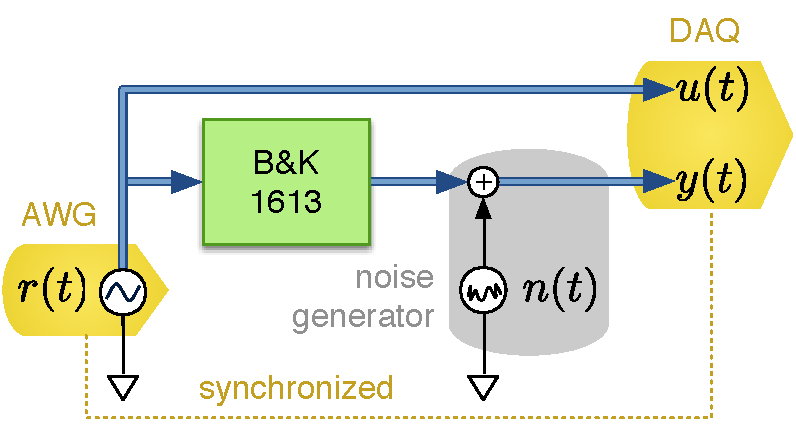
\includegraphics[width=0.6\columnwidth]{\thisDir/figs/measurement.pdf}
  \caption[Measurement schematic of \BK\ 1613 filter.]{Schematic representation of the measurement set-up for the \BK\ 1613 filter. The AWG (Arbitrary Waveform Generator) and DAQ (Data Acquisition) hardware share the same clock and are thus synchronized. 
  Blue arrows indicate coax cables. 
  At the output of the bandpass filter, a noise generator is added that buffers the incoming signal using a TL071 opamp and adds white noise before passing the signal to the DAQ.} 
  \label{fig:measurementSetup}
\end{figure}


To measure the transfer function, the \BK{} 1613 Filter was excited by a signal $r(t)$ and both its input $u(t)$ and output $y(t)$ were measured as shown in \figref{fig:measurementSetup}.
The output $y(t)$, however, was disturbed by a noise generator that added white noise over the frequency range $[\mathrm{DC}, 20\unit{kHz}]$.
The excitation signal $r(t)$ was white random noise with a standard deviation $\sigma_r = 0.25 \unit{V}$, consisting of $N_S = 8\,192$ samples, and sampled at $92 \unit{kHz}$.
The same noise sequence was repeated $N_R = 100$ times in succession, such that a non-parametric estimate of the noise could be obtained and the performance of the methods could be gauged over these different repetitions.
To distinguish the different repetitions, we denote the $r^{\text{th}}$ repetition of the $u$ signal as $u^{[r]}(t)$ (and similarly for $y(t)$).
The signal generation and acquisition was by means of a \gls{NI} Elvis II, using the respective \code{AO} and \code{AI} pins on the breadboard, which were wired to BNC connectors.
Although acquisition and generation were synchronized, there is a small delay $\tau_{\mathrm{MUX}} \approx 9\unit{\mu s}$ between the acquisition of the input $u(t)$ and the output $y(t)$ due to the hardware architecture of the \gls{NI} Elvis II.
Particularly, the involved channels are captured by means of a single \gls{ADC} which is preceded by a multiplexer to select the active channel.
This obviously introduces a slight delay between the acquisition of a sample of input and output channels that is not part of system dynamics of the \BK{} filter, but rather of the experimental set-up.
As such, the output spectrum $Y(\omega)$ was multiplied by $\exp\left(-j\omega\tau_{\mathrm{MUX}} \right)$ such that this inter-channel acquisition delay of the \gls{NI} Elvis is compensated; the time-domain counterpart $y(t)$ is obtained using the \gls{IDFT}.

\begin{figure}
  \centering
  \setlength{\figurewidth}{0.75\columnwidth}
  \setlength{\figureheight}{0.68\figurewidth}
  % This file was created by matlab2tikz.
%
%workdir  : /Users/egon/Dropbox/VUB/PhD/Mikaya/initialvalues
%git info : commit 738172a88e3110ebbaa770c63b1b0198fe9ecd02
%           Author: Egon Geerardyn <egon.geerardyn@gmail.com>
%           Date:   Tue Feb 16 20:07:07 2016 +0100
%           
%               Revert to actual timing mode
%           
%            testRuntimes.m | 4 ++--
%            1 file changed, 2 insertions(+), 2 deletions(-)
%           
%
%
% \definecolor{mycolor1}{rgb}{0.00000,1.00000,1.00000}%
% \definecolor{mycolor2}{rgb}{1.00000,1.00000,0.00000}%
% %
% \begin{tikzpicture}

% \begin{axis}[%
% width=0.951\figurewidth,
% height=\figureheight,
% at={(0\figurewidth,0\figureheight)},
% scale only axis,
% xmode=log,
% xmin=1000,
% xmax=16000,
% ymin=-70,
% ymax=10,
% axis background/.style={fill=white},
% axis x line*=bottom,
% axis y line*=left,
% legend style={legend cell align=left,align=left,draw=white!15!black}
% ]
% \addplot [color=mycolor1,only marks,mark=*,mark options={solid}]
%   table[]{fig/bode-bk1613-1.tsv};
% \addlegendentry{Y/U};

% \addplot [color=blue,only marks,mark=*,mark options={solid}]
%   table[]{fig/bode-bk1613-2.tsv};
% \addlegendentry{mean Y/U};

% \addplot [color=green,only marks,mark=*,mark options={solid}]
%   table[]{fig/bode-bk1613-3.tsv};
% \addlegendentry{$\text{G}_{\text{VXI}}\text{ (normal)}$};

% \addplot [color=mycolor2,only marks,mark=*,mark options={solid}]
%   table[]{fig/bode-bk1613-4.tsv};
% \addlegendentry{$\text{G}_{\text{VXI}}\text{ (extra delay)}$};

% \addplot [color=black,solid]
%   table[]{fig/bode-bk1613-5.tsv};
% \addlegendentry{$\text{G}_{\text{ds}}$};

% \addplot [color=red,solid]
%   table[]{fig/bode-bk1613-6.tsv};
% \addlegendentry{$\text{G}_{\text{VXI}}$};

% \end{axis}
% \end{tikzpicture}%

\begin{tikzpicture}
\begin{axis}[%
width=\figurewidth,
height=\figureheight,
unbounded coords=jump,
xlabel={Frequency \axisunit{Hz}},
ylabel={Amplitude $\left| G \right|$ \axisunit{dB}},
scale only axis,
xmode=log,
grid=both,
yminorticks=true,
extra x ticks={4000},
extra x tick labels={$4000^{\vphantom{1}}$},
extra y ticks={10},
extra y tick labels={},
xmin=400,
xmax=40000,
xminorticks=true,
ymin=-80,
ymax=10,
axis x line*=bottom,
axis y line*=left]

\addplot [FRFSingle,forget plot]
  table[]{\thisDir/fig/bode-bk1613-ETFE-single.tsv};
%\addlegendentry{Y/U};
\label{leg:bk1613:ETFE}

\addplot [FRFMean,forget plot]
  table[]{\thisDir/fig/bode-bk1613-ETFE-mean.tsv};
% %\addlegendentry{mean Y/U};
\label{leg:bk1613:meanETFE}

\addplot [GVXI,mark=*,extremelytinymarkers]
  table[]{\thisDir/fig/bode-bk1613-GVXI.tsv};
%\addlegendentry{$\text{G}_{\text{VXI}}$};
\label{leg:bk1613:vxi}

\end{axis}
\end{tikzpicture}%

  \caption[\BK{} 1613 filter transfer function]{Transfer function of the considered \BK{} 1613 filter.
  The empirical transfer function estimates $Y^{[r]}(\omega)/U^{[r]}(\omega)$~\legref{leg:bk1613:ETFE} and its average $\tilde{Y}(\omega)/\tilde{U}(\omega)$~\legref{leg:bk1613:meanETFE} obtained from the Elvis measurements are shown together with the estimated reference model $G_{\mathrm{VXI}}$~\legref{leg:bk1613:vxi}.} 
  \label{fig:bk1613}
\end{figure}


\subsection{Identification Procedure}
The repeated nature of the experiment makes it possible to estimate the noise level from the signals non-parametrically.
The mean signal from the input $u$ is of the form:
\begin{equation}
  \tilde{u}(t) = \frac{1}{N_R} \sum_{r=1}^{N_R} u^{[r]}(t)
\end{equation}
Thus, the reduced noise influence and the approximate noise co-variances are, respectively:
\begin{align}
  \hat\sigma_{u}^2(t) &= \frac{1}{N_R - 1} 
                    \sum_{r=1}^{N_R} 
                    \left( u^{[r]}(t) - \tilde{u}(t) \right)^2 \\
%and the noise co-variances are approximately
  \hat\sigma_{yu}(t) &= \frac{1}{N_R - 1} 
                    \sum_{r=1}^{N_R} 
                    \left( y^{[r]}(t) - \tilde{y}(t) \right)
                    \overline{\left( u^{[r]}(t) - \tilde{u}(t) \right)}
  \label{eq:variancePeriodic}            
\end{align}
 
Similar calculations apply to $y(t)$ and as such, $\hat\sigma_u(t)$, $\hat\sigma_y(t)$ and $\hat\sigma_{yu}(t)$ can be estimated.
Their frequency domain counterparts $\tilde{U}(\omega)$ and $\tilde{Y}(\omega)$ are obtained by using the DFT.
The resulting empirical transfer function estimate $Y^{[r]}(\omega)/U^{[r]}(\omega)$ and its periodic average $\tilde{Y}/\tilde{U}$ are shown in \figref{fig:bk1613}.
The noise covariances $\hat\sigma^2_{U}(\omega)$, $\hat\sigma^2_{Y}(\omega)$ and  $\hat\sigma_{YU}(\omega)$ are calculated as the sample covariance, akin to equation \eqref{eq:variancePeriodic}, and their values are shown in \figref{fig:SpectraMeasurement}.
Note that the SNR at the output $\mathrm{SNR}_{y} \approx 14 \unit{dB}$ is much smaller than at the input $\mathrm{SNR}_{u} \approx 50 \unit{dB}$.

\begin{figure}
  \centering
  \setlength{\figurewidth}{0.75\columnwidth}
  \setlength{\figureheight}{0.68\figurewidth}
  % This file was created by matlab2tikz v0.4.7 (commit 742c12da8070045a639367962f5a55fd750c0cae) running on MATLAB 8.3.
% Copyright (c) 2008--2014, Nico Schlömer <nico.schloemer@gmail.com>
% All rights reserved.
% Minimal pgfplots version: 1.3
% 
% workdir  : /Users/egon/Dropbox/VUB/PhD/Mikaya/InitialValues
% git info : commit 45c2d89a4e4044db9de2834c5c1c86bec69e4864
%            Author: Egon Geerardyn <egon.geerardyn@gmail.com>
%            Date:   Tue Oct 7 09:18:45 2014 +0200
%            
%                estimParamMeas: duplicate code removed
%            
%             estimateParametricMeas.m | 9 +--------
%             1 file changed, 1 insertion(+), 8 deletions(-)
%            
% 
% 
%
\begin{tikzpicture}
\begin{axis}[%
width=0.5\figurewidth,
height=\figureheight,
scale only axis,
xmin=400,
xmax=40000,
grid=both,
xmode=log,
xlabel={Frequency (Hz)},
ymin=-50,
ymax=40,
ylabel={$\left|U(\omega)\right|$ \axisunit{dB_{V}}},
name=Uspectrum,
axis x line*=bottom,
axis y line*=left
]
% \addplot [FRFSingle,forget plot]
%     table{\thisDir/fig/elvis-spectra-1.tsv};
% \label{leg:SpectraMeasurement:U:single}
\addplot [FRFNoise,forget plot]
  table{\thisDir/fig/elvis-spectra-3.tsv};
\label{leg:SpectraMeasurement:U:noise}
\addplot [FRFMean,forget plot]
  table{\thisDir/fig/elvis-spectra-2.tsv};
\label{leg:SpectraMeasurement:U:mean}
\end{axis}
\begin{axis}[%
anchor=left of north west,
at=(Uspectrum.right of north east),
xshift=0.5em,
width=0.5\figurewidth,
height=\figureheight,
scale only axis,
grid=both,
xmin=400,
xmax=40000,
xmode=log,
xlabel={Frequency \axisunit{Hz}},
ymin=-50,
ymax=40, 
ylabel={$\left|Y(\omega)\right|$ \axisunit{dB_{V}}},
yticklabels={},
axis x line*=bottom,
axis y line*=right
]
% \addplot [FRFSingle,forget plot]
%   table{\thisDir/fig/elvis-spectra-4.tsv};
\addplot [FRFNoise,forget plot]
  table{\thisDir/fig/elvis-spectra-6.tsv};
\addplot [FRFMean,forget plot]
  table{\thisDir/fig/elvis-spectra-5.tsv};
\end{axis}
\end{tikzpicture}%

  \caption[Measured input/output spectra of \BK{} filter.]{Average input $\tilde{U}(\omega)$ and output $\tilde{Y}(\omega)$ spectra \legref[2]{leg:SpectraMeasurement:U:mean} measured using the Elvis and the noise levels $\hat\sigma_U$ and $\hat\sigma_Y$  \legref[2]{leg:SpectraMeasurement:U:noise}.}
  \label{fig:SpectraMeasurement}
\end{figure}

For each measurement repetition, the signals $u^{[r]}(t)$, $y^{[r]}(t)$ and the variances $\sigma_U^2(\omega)$, $\sigma_Y^2(\omega)$ are used in the maximum likelihood cost function given by equation \eqref{eq:MLEcf}.
The model order was chosen according to the specifications of the sixth-order (Chebyshev) bandpass filter \citep{datasheet_bk1613}.
Since such a bandpass filter is of sixth degree and requires a relative degree of 3 to produce a $60 \unit{dB/decade}$ slope at high frequencies, this means that the transfer function has a numerator of third order, a denominator of sixth order and transient contribution of a fifth degree (i.e. model order: $3/6+5$).
This results in a transfer function of the form:
\begin{equation}
  \model{\bullet}(s,\theta) = 
  \frac{\Sum_{i=0}^3 b_i s^i}{\Sum_{i=0}^6 a_i s^i}
\end{equation}
which is typical of a sixth-order band-pass filter.
By processing the different repetitions, a parametric fit per initialization method corresponding to the appropriate branch in \figref{fig:flowgraph}, and per repetition can be obtained. 
\begin{remark}
Fitting the data with models of increased order (e.g. $4/6+5$) has also been attemped, but those models did not yield significant improvements.
\end{remark}


The following equation is constructed from the final estimates for each experiment; it gives an insight into the combined contribution to the `best' estimate from all the different initialization strategies, \emph{viz}:

\begin{equation}\label{eq:selectBest}
  \model{best} = 
    \Arg_{\hat{G}} 
    \min 
    \left\{ 
      V(\model{exist}),
      V(\model{trunc}),
      V(\model{RFIR})
    \right\}
\end{equation}
where $V(\hat{G})$ corresponds to the cost function in equation \eqref{eq:MLEcf} in the parametric estimates of $\hat{G}$.
This is similar to the approach followed in~\citep{FDIDENT} to combine different initial estimates.

Alternatively, one can define the best model ($\model{best}$) and the second best model ($\model{2nd}$) as the models that comply to the inequalty
$
  \costFunc{}\left(\model{best}\right) < 
  \costFunc{}\left( \model{2nd} \right) < 
  \ldots
$
where $\model{best} \neq \model{2nd}$.

\subsection{Reference Model Measurements}

%\JL{
Since the true model $\true{G}$ is not known for real-life systems, a practically viable reference model is needed.
Additional measurements were performed using a \gls{VXI} measurement setup, which allowed for a signal-to-noise ratio of more than $60\unit{dB}$. 
Virtually noiseless, these measurements provided a very high quality model of the system, denoted as $G_\mathrm{VXI}$, and used as a reference model. 
The \gls{VXI} measurement setup is summarized as follows.
\begin{itemize}
  \item Signal Generator card: \gls{VXI} HP E1445A.
  \item Acquisition cards: \gls{VXI} HP E1430A.
  \item Sampling frequency: $f_\mathrm{s} = 156\,250 \unit{Hz}$.
  \item A total of $558$ frequency bins were used for the estimation, in the excited frequency band $[0.1,20] \unit{kHz}$, with a frequency resolution of $35.7\unit{Hz}$, giving a measurement time of $28\unit{ms}$. The excitation signal was band-limited periodic noise with an \gls{RMS} of $100\unit{mV}$.
  \item The input and output signals were buffered and anti-alias filtered.
\end{itemize}
This yielded the model $G_\mathrm{VXI}$ (shown in \figref{fig:bk1613}) with a relative error  of less than $0.3\%$ in the pass-band.  Denote $\model{VXI}$ to be the parametric estimate obtained using $G_{\mathrm{VXI}}$ as an initial estimate. Furthermore, $G_\mathrm{VXI}$ was used to play the role of $\true{G}$ from the previous section.

\subsection{Model Estimation}
  The measurements on the NI Elvis II indicate that the high-quality starting value $G_{\mathrm{VXI}}$ led to low cost function values as shown in \figref{fig:costMeasurements} and \tabref{tbl:costMeasurements}.
  The existing methods exhibit a high spread and a high median cost function, showing that a good estimate is obtained only in about $25\%$ of the cases.
  The truncation method provides better estimates in many cases, but still suffers from a high variability.
  On the other hand, the \gls{RFIR}-based initial values have both a low median cost function and spread, and thus provide better fits in almost all cases.
  Obviously, $\model{best}$ has the lowest cost function values of all methods.
  The similarity of the results for $\model{RFIR}$ and $\model{best}$ suggests that the \gls{RFIR} provides the best estimate in most of the cases.
  This can indeed be confirmed by inspecting the different estimates per repetition of the experiment.

\begin{remark}
  In the simulations (e.g. \figref{fig:single-sim}), a $60\unit{dB}$ difference between `good' and `bad' estimates was observed.
  Such a large gap is not observed in the measurements (\figref{fig:costMeasurements} and \tabref{tbl:costMeasurements}).
  Hence, defining a success rate based on a threshold tolerance would be very sensitive to the specific value of the threshold and hence unreliable.
  Instead, the statistical location and dispersion are inspected to assess the relative performance of each method.
  Practically, the median is used as a measure of location and the \gls{IQR} is used to inspect the spread as these are far more robust to outliers than e.g. the sample mean and variance.
  These measures also have an easy interpretation: the median ($50\%$ percentile) indicates the cost function value that $50\%$ of the repetitions attain.
  On the other hand, the \gls{IQR} ($25\%$ through $75\%$ percentile) contains  exactly half of the observations.
\end{remark}

\begin{figure}[p]
  \centering
  \setlength{\figurewidth}{0.85\columnwidth}
  \setlength{\figureheight}{0.68\figurewidth}
  \setlength{\figurewidth}{0.75\columnwidth}
  % This file was created by matlab2tikz v0.4.7 (commit 531759ea1f2f805c5b2ec975ee93dc15fff84184) running on MATLAB 8.3.
% Copyright (c) 2008--2014, Nico Schlömer <nico.schloemer@gmail.com>
% All rights reserved.
% Minimal pgfplots version: 1.3
% 
% workdir  : /Users/egon/Dropbox/VUB/PhD/Mikaya/InitialValues
% git info : commit f9bbeb38f35d63f56a82a16c2145c8bd72f1e461
%            Author: Egon Geerardyn <egon.geerardyn@gmail.com>
%            Date:   Thu Oct 2 13:07:09 2014 +0200
%            
%                Proc meas with noise
%            
%             processAllMeasurements.m | 37 +++++++++++++++++++++++++------------
%             1 file changed, 25 insertions(+), 12 deletions(-)
%            
% 
% 
%
% defining custom colors
\begin{tikzpicture}

\begin{axis}[%
width=\figurewidth,
height=0.5\figureheight,
scale only axis,
xmin=0.5,
xmax=5.5,
name=global,
xtick={0.5,1.5,2.5,3.5,4.5,5.5},
xticklabels={{$\model{VXI}$},
             {$\model{exist}$},
             {$\model{trunc}$},
             {$\model{RFIR}$},
             {$\model{best}$}},
% extra x ticks={5.5},
% extra x tick labels={},
x tick label as interval,
xticklabels={},
ymode=log,
ymin=4000,
ymax=1e5,
yminorticks=true,
ymajorgrids=true,
yminorgrids=true,
xmajorgrids=true,
ylabel={Cost $V(\theta)$},
axis x line*=bottom,
axis y line*=left
]

\addplot [boxplotBox,fill=G0HatFill,forget plot] table {\thisDir/data/meas-cost/CostFunctionsMLE-measurement-1.tsv};
\addplot [boxplotQuantiles,color=G0Hat,forget plot] table{\thisDir/data/meas-cost/CostFunctionsMLE-measurement-2.tsv};
\addplot [individualSamples,G0Hat,G0Hatmark,forget plot] table{\thisDir/data/meas-cost/CostFunctionsMLE-measurement-3.tsv};

\addplot [boxplotBox,fill=existingFill,forget plot] table {\thisDir/data/meas-cost/CostFunctionsMLE-measurement-4.tsv};
\addplot [boxplotQuantiles,color=existing,forget plot] table{\thisDir/data/meas-cost/CostFunctionsMLE-measurement-5.tsv};
\addplot [individualSamples,existing,existingmark,forget plot] table{\thisDir/data/meas-cost/CostFunctionsMLE-measurement-6.tsv};

\addplot [boxplotBox,fill=LPMTruncFill,forget plot] table {\thisDir/data/meas-cost/CostFunctionsMLE-measurement-7.tsv};
\addplot [boxplotQuantiles,color=LPMTrunc,forget plot] table{\thisDir/data/meas-cost/CostFunctionsMLE-measurement-8.tsv};
\addplot [individualSamples,LPMTrunc,LPMTruncmark,forget plot] table{\thisDir/data/meas-cost/CostFunctionsMLE-measurement-9.tsv};

\addplot [boxplotBox,fill=RFIRFill,forget plot] table {\thisDir/data/meas-cost/CostFunctionsMLE-measurement-10.tsv};
\addplot [boxplotQuantiles,color=RFIR,forget plot] table{\thisDir/data/meas-cost/CostFunctionsMLE-measurement-11.tsv};
\addplot [individualSamples,RFIR,RFIRmark,forget plot] table{\thisDir/data/meas-cost/CostFunctionsMLE-measurement-12.tsv};

\addplot [boxplotBox,fill=bestFill,forget plot] table {\thisDir/data/meas-cost/CostFunctionsMLE-measurement-13.tsv};
\addplot [boxplotQuantiles,color=best,forget plot] table{\thisDir/data/meas-cost/CostFunctionsMLE-measurement-14.tsv};
\addplot [individualSamples,best,bestmark,forget plot] table{\thisDir/data/meas-cost/CostFunctionsMLE-measurement-15.tsv};
\end{axis}

\begin{axis}[%
width=\figurewidth,
height=0.5\figureheight,
name=detail,
anchor=north west,
at={($(global.south west) - (0pt,1.5em)$)},
scale only axis,
xmin=0.5,
xmax=5.5,
xtick={0.5,1.5,2.5,3.5,4.5,5.5},
xticklabels={{$\model{VXI}$},
             {$\model{exist}$},
             {$\model{trunc}$},
             {$\model{RFIR}$},
             {$\model{best}$}},
extra y ticks={9000},
extra y tick labels={},
scaled y ticks=false,
x tick label as interval,
ymin=4000,
ymax=9000,
yminorticks=true,
ymajorgrids=true,
yminorgrids=true,
xmajorgrids=true,
ylabel={Cost $V(\theta)$},
axis x line*=bottom,
axis y line*=left
]

\addplot [boxplotBox,fill=G0HatFill,forget plot] table {\thisDir/data/meas-cost/CostFunctionsMLE-measurement-1.tsv};
\addplot [boxplotQuantiles,color=G0Hat,forget plot] table{\thisDir/data/meas-cost/CostFunctionsMLE-measurement-2.tsv};
\addplot [individualSamples,G0Hat,G0Hatmark,forget plot] table{\thisDir/data/meas-cost/CostFunctionsMLE-measurement-3.tsv};

\addplot [boxplotBox,fill=existingFill,forget plot] table {\thisDir/data/meas-cost/CostFunctionsMLE-measurement-4.tsv};
\addplot [boxplotQuantiles,color=existing,forget plot] table{\thisDir/data/meas-cost/CostFunctionsMLE-measurement-5.tsv};
\addplot [individualSamples,existing,existingmark,forget plot] table{\thisDir/data/meas-cost/CostFunctionsMLE-measurement-6.tsv};

\addplot [boxplotBox,fill=LPMTruncFill,forget plot] table {\thisDir/data/meas-cost/CostFunctionsMLE-measurement-7.tsv};
\addplot [boxplotQuantiles,color=LPMTrunc,forget plot] table{\thisDir/data/meas-cost/CostFunctionsMLE-measurement-8.tsv};
\addplot [individualSamples,LPMTrunc,LPMTruncmark,forget plot] table{\thisDir/data/meas-cost/CostFunctionsMLE-measurement-9.tsv};

\addplot [boxplotBox,fill=RFIRFill,forget plot] table {\thisDir/data/meas-cost/CostFunctionsMLE-measurement-10.tsv};
\addplot [boxplotQuantiles,color=RFIR,forget plot] table{\thisDir/data/meas-cost/CostFunctionsMLE-measurement-11.tsv};
\addplot [individualSamples,RFIR,RFIRmark,forget plot] table{\thisDir/data/meas-cost/CostFunctionsMLE-measurement-12.tsv};

\addplot [boxplotBox,fill=bestFill,forget plot] table {\thisDir/data/meas-cost/CostFunctionsMLE-measurement-13.tsv};
\label{leg:costMeasurements:best:iqr}
\addplot [boxplotQuantiles,color=best,forget plot] table{\thisDir/data/meas-cost/CostFunctionsMLE-measurement-14.tsv};
\label{leg:costMeasurements:best:median}
\addplot [individualSamples,best,bestmark,forget plot] table{\thisDir/data/meas-cost/CostFunctionsMLE-measurement-15.tsv};
\label{leg:costMeasurements:best:data}

\end{axis}
\end{tikzpicture}%

  \caption[Cost function values over the different measurements.]{Cost function values $V(\theta)$ obtained during the different realizations of the measurement.
  The bottom plot shows a linear zoom of the top plot.
  For each method, the inter-quartile range~\legref{leg:costMeasurements:best:iqr}, median~\legref{leg:costMeasurements:best:median} and individual values~\legref{leg:costMeasurements:best:data} are shown.
  This implies that a lower (local) minimum of the cost function can be attained using these smoothing techniques.}
  \label{fig:costMeasurements}
\end{figure}

\begin{table}[p]
  \centering
  \caption{Observed percentiles of the cost function $V(\model{\bullet}$).}
  \pgfplotstabletypeset[precision=0]{
method            P000     P025     P050      P075       P100   
\model{VXI}       4354.83  4442.31  4493.52   4706.61    9633.53
\model{exist}     4345.3   4525.82  8740.54  12413.3    29236.5
\model{trunc}     4335.68  4476.29  4841.74   8130.28   88308.1
\model{RFIR}      4328.93  4422.11  4468.8    4716.46    9606.54
\model{best}      4328.93  4414.87  4457.91   4644.07    8569.93 
}

  \label{tbl:costMeasurements}
\end{table}



\subsection{Model Validation}
\subsubsection{Cost Function Limitations}
In the previous section, the cost function was studied to determine the effectiveness of the starting values.
However, inspecting the cost function $V(\theta)$ only accounts for how well an estimated model fits the measured data, which may be misleading.
For an example, overfitting a model may result in the absorption of both the systematic behavior and the noise into the model. 
Consequently, an arbitrarily small cost function may ensue although the estimated model may be virtually useless to predict the system behavior.

\subsubsection{Validation Criterion}
To objectively assess the quality of an estimated model, a different criterion than the cost function is inspected.
To this end, the model is validated using the 2-norm (or distance) on the model error:
\begin{equation}
  \validationDistance{\bullet} 
  \isdef 
  \norm[2]{\model{\bullet} - G_{\mathrm{VXI}}}
  \text{.}
  \label{eq:measurementCriterion}
\end{equation} 
This criterion indicates how well the obtained estimates $\model{\bullet}$ are able to describe the transfer function of the bandpass filter as observed in the validation measurement on the \gls{VXI}.

\subsubsection{Validation Performance}
The observed median and \gls{IQR} of the distances in \figref{fig:validationMeasurements} and \tabref{tbl:validationMeasurements} have a similar qualitative interpretation as the cost function on the estimation data.
The existing methods provide good estimates in only $25\%$ of the cases.
The truncation method provides a considerable improvement but still suffers from $25\%$ poor estimates.
Compared to the existing \gls{BTLS} and \gls{GTLS} techniques, the \gls{RFIR} and hence also $\model{best}$ entail an overall reduction in the observed distance by a factor $8$, in most cases. 
On the other hand, the reference $\model{VXI}$ shows the best global performance. 
This indicates that the proposed methods do no converge to the same local optimum.
Nevertheless, the proposed methods improve the model quality by almost an order of magnitude.

As the criterion in equation~\eqref{eq:measurementCriterion} no longer depends on the cost function, the initial estimates can also be investigated.
The difference between the distance of $\model[init]{\bullet}$ and $\model{\bullet}$ indicates how much the final ML estimate from the raw data, in each respective branch of \figref{fig:flowgraph}, improves over the initial estimate.
Remarkably, on average, the final ML estimation provides only a marginal improvement for the \gls{RFIR}. 
However, this final step reduces the spread and hence yields a more reliable estimate.
E.g. note in \tabref{tbl:validationMeasurements} that this step reduces the worst-case distance from $18.21$ to $4.55$.


\begin{figure}[p]
  \centering
  \setlength{\figurewidth}{0.85\columnwidth}
  \setlength{\figureheight}{0.68\figurewidth}
  \setlength{\figurewidth}{0.75\columnwidth}
  % This file was created by matlab2tikz v0.4.7 (commit 742c12da8070045a639367962f5a55fd750c0cae) running on MATLAB 8.3.
% Copyright (c) 2008--2014, Nico Schlömer <nico.schloemer@gmail.com>
% All rights reserved.
% Minimal pgfplots version: 1.3
% 
% workdir  : /Users/egon/Dropbox/VUB/PhD/Mikaya/InitialValues
% git info : commit 45c2d89a4e4044db9de2834c5c1c86bec69e4864
%            Author: Egon Geerardyn <egon.geerardyn@gmail.com>
%            Date:   Tue Oct 7 09:18:45 2014 +0200
%            
%                estimParamMeas: duplicate code removed
%            
%             estimateParametricMeas.m | 9 +--------
%             1 file changed, 1 insertion(+), 8 deletions(-)
%            
% 
% 
%
% defining custom colors
\begin{tikzpicture}

\begin{axis}[%
name=global,
width=\figurewidth,
height=0.5\figureheight,
scale only axis,
xmin=0.5,
xmax=7.5,
x tick label as interval,
xtick={0.5,1.5,2.5,3.5,4.5,5.5,6.5,7.5},
xticklabels={{$\model{VXI}$},
             {$\model{exist}$},
             {$\model{trunc}^{\mathrm{init}}$},
             {$\model{trunc}$},
             {$\model{RFIR}^{\mathrm{init}}$},
             {$\model{RFIR}$},
             {$\model{best}$}},
xticklabels={},
ymode=log,
ymin=0.4,
ymax=100,
yminorticks=true,
grid=both,
% extra y ticks={120},
% extra y tick labels={},
ylabel={$\norm[2]{\model{\bullet} - G_{\mathrm{VXI}} }$},
axis x line*=bottom,
axis y line*=left
]
\addplot[dashed, black, forget plot] table[row sep=crcr]{%
0   81.555\\
10  81.555\\
};
\label{leg:validationMeasurements:H2Norm}

\addplot[area legend,solid,fill=G0HatFill,opacity=0.7,draw=none,forget plot]
table {\thisDir/fig/data/meas-validation/meas-validation-1.tsv};

\addplot [color=G0Hat,solid,forget plot]
  table{\thisDir/fig/data/meas-validation/meas-validation-2.tsv};
\addplot [G0Hat,G0Hatmark,tinymarkers,opacity=0.7,only marks,forget plot]
  table{\thisDir/fig/data/meas-validation/meas-validation-3.tsv};

\addplot[area legend,solid,fill=existingFill,opacity=0.7,draw=none,forget plot]
table {\thisDir/fig/data/meas-validation/meas-validation-4.tsv};

\addplot [color=existing,solid,forget plot]
  table{\thisDir/fig/data/meas-validation/meas-validation-5.tsv};
\addplot [existing,existingmark,tinymarkers,opacity=0.7,only marks,forget plot]
  table{\thisDir/fig/data/meas-validation/meas-validation-6.tsv};

\addplot[area legend,opacity=0.15,fill=LPMTruncInit,draw=none,forget plot]
table {\thisDir/fig/data/meas-validation/meas-validation-7.tsv};

\addplot [LPMTruncInit,solid,forget plot]
  table{\thisDir/fig/data/meas-validation/meas-validation-8.tsv};
\addplot [LPMTruncInitmark,color=LPMTruncInit,tinymarkers,opacity=0.7,only marks,forget plot]
  table{\thisDir/fig/data/meas-validation/meas-validation-9.tsv};

\addplot[area legend,solid,fill=LPMTruncFill,opacity=0.7,draw=none,forget plot]
table {\thisDir/fig/data/meas-validation/meas-validation-10.tsv};

\addplot [color=LPMTrunc,solid,forget plot]
  table{\thisDir/fig/data/meas-validation/meas-validation-11.tsv};
\addplot [LPMTrunc,LPMTruncmark,tinymarkers,opacity=0.7,only marks,forget plot]
  table{\thisDir/fig/data/meas-validation/meas-validation-12.tsv};

\addplot[area legend,opacity=0.15,fill=RFIRInit,draw=none,forget plot]
table {\thisDir/fig/data/meas-validation/meas-validation-13.tsv};

\addplot [RFIRInit,solid,forget plot]
  table{\thisDir/fig/data/meas-validation/meas-validation-14.tsv};
\addplot [RFIRInit,RFIRInitmark,tinymarkers,opacity=0.7,only marks,forget plot]
  table{\thisDir/fig/data/meas-validation/meas-validation-15.tsv};

\addplot[area legend,solid,fill=RFIRFill,opacity=0.7,draw=none,forget plot]
table {\thisDir/fig/data/meas-validation/meas-validation-16.tsv};

\addplot [color=RFIR,solid,forget plot]
  table{\thisDir/fig/data/meas-validation/meas-validation-17.tsv};
\addplot [RFIR,RFIRmark,tinymarkers,only marks,opacity=0.7,forget plot]
  table{\thisDir/fig/data/meas-validation/meas-validation-18.tsv};

\addplot[area legend,solid,fill=bestFill,opacity=0.7,draw=none,forget plot]
table {\thisDir/fig/data/meas-validation/meas-validation-19.tsv};
\label{leg:validationMeasurements:best:iqr}

\addplot [color=best,solid,forget plot]
  table{\thisDir/fig/data/meas-validation/meas-validation-20.tsv};
\label{leg:validationMeasurements:best:median}
\addplot [best,bestmark,tinymarkers,only marks,opacity=0.7,forget plot]
  table{\thisDir/fig/data/meas-validation/meas-validation-21.tsv};
\label{leg:validationMeasurements:best:data}
\end{axis}

\begin{axis}[%
name=detail,
anchor=north west,
at={($(global.south west) - (0pt,1.5em)$)},
width=\figurewidth,
height=0.5\figureheight,
scale only axis,
xmin=0.5,
xmax=7.5,
x tick label as interval,
xtick={0.5,1.5,2.5,3.5,4.5,5.5,6.5,7.5},
xticklabels={{$\model{VXI}$},
             {$\model{exist}$},
             {$\model[init]{trunc}$},
             {$\model{trunc}$},
             {$\model[init]{RFIR}$},
             {$\model{RFIR}$},
             {$\model{best}$}},
ymin=0.45,
ymax=3,
yminorticks=true,
grid=major,
%extra y ticks={30},
%extra y tick labels={},
ylabel={$\norm[2]{\model{\bullet} - G_{\mathrm{VXI}} }$},
axis x line*=bottom,
axis y line*=left
]

\addplot[area legend,solid,fill=G0HatFill,opacity=0.7,draw=none,forget plot]
table {\thisDir/fig/data/meas-validation/meas-validation-1.tsv};

\addplot [color=G0Hat,solid,forget plot]
  table{\thisDir/fig/data/meas-validation/meas-validation-2.tsv};
\addplot [G0Hat,G0Hatmark,tinymarkers,opacity=0.7,only marks,forget plot]
  table{\thisDir/fig/data/meas-validation/meas-validation-3.tsv};

\addplot[area legend,solid,fill=existingFill,opacity=0.7,draw=none,forget plot]
table {\thisDir/fig/data/meas-validation/meas-validation-4.tsv};

\addplot [color=existing,solid,forget plot]
  table{\thisDir/fig/data/meas-validation/meas-validation-5.tsv};
\addplot [existing,existingmark,tinymarkers,opacity=0.7,only marks,forget plot]
  table{\thisDir/fig/data/meas-validation/meas-validation-6.tsv};

\addplot[area legend,opacity=0.15,fill=LPMTruncInit,draw=none,forget plot]
table {\thisDir/fig/data/meas-validation/meas-validation-7.tsv};

\addplot [LPMTruncInit,solid,forget plot]
  table{\thisDir/fig/data/meas-validation/meas-validation-8.tsv};
\addplot [LPMTruncInitmark,color=LPMTruncInit,tinymarkers,opacity=0.7,only marks,forget plot]
  table{\thisDir/fig/data/meas-validation/meas-validation-9.tsv};

\addplot[area legend,solid,fill=LPMTruncFill,opacity=0.7,draw=none,forget plot]
table {\thisDir/fig/data/meas-validation/meas-validation-10.tsv};

\addplot [color=LPMTrunc,solid,forget plot]
  table{\thisDir/fig/data/meas-validation/meas-validation-11.tsv};
\addplot [LPMTrunc,LPMTruncmark,tinymarkers,opacity=0.7,only marks,forget plot]
  table{\thisDir/fig/data/meas-validation/meas-validation-12.tsv};

\addplot[area legend,opacity=0.15,fill=RFIRInit,draw=none,forget plot]
table {\thisDir/fig/data/meas-validation/meas-validation-13.tsv};

\addplot [RFIRInit,solid,forget plot]
  table{\thisDir/fig/data/meas-validation/meas-validation-14.tsv};
\addplot [RFIRInit,RFIRInitmark,tinymarkers,opacity=0.7,only marks,forget plot]
  table{\thisDir/fig/data/meas-validation/meas-validation-15.tsv};

\addplot[area legend,solid,fill=RFIRFill,opacity=0.7,draw=none,forget plot]
table {\thisDir/fig/data/meas-validation/meas-validation-16.tsv};

\addplot [color=RFIR,solid,forget plot]
  table{\thisDir/fig/data/meas-validation/meas-validation-17.tsv};
\addplot [RFIR,RFIRmark,tinymarkers,only marks,opacity=0.7,forget plot]
  table{\thisDir/fig/data/meas-validation/meas-validation-18.tsv};

\addplot[area legend,solid,fill=bestFill,opacity=0.7,draw=none,forget plot]
table {\thisDir/fig/data/meas-validation/meas-validation-19.tsv};

\addplot [color=best,solid,forget plot]
  table{\thisDir/fig/data/meas-validation/meas-validation-20.tsv};
\addplot [best,bestmark,tinymarkers,only marks,opacity=0.7,forget plot]
  table{\thisDir/fig/data/meas-validation/meas-validation-21.tsv};
\end{axis}
\end{tikzpicture}%

  \caption[Validation cost of the different measurements.]{Validation of the measured models. 
  For each method, the distance \eqref{eq:measurementCriterion} between the estimates and $\model{VXI}$ is shown~\legref{leg:validationMeasurements:best:data} together with the median~\legref{leg:validationMeasurements:best:median} and inter-quartile range~\legref{leg:validationMeasurements:best:iqr}.
  $\norm{G_{\mathrm{VXI}}}$\legref{leg:validationMeasurements:H2Norm} is shown as a reference.
  The bottom plot shows a linear zoom of the top plot.
  The proposed methods yield models that are closer to $\model{VXI}$ than the existing $\model{exist}$.
  The results are in line with the values of the cost function in \figref{fig:costMeasurements}.}
  \label{fig:validationMeasurements}
\end{figure}
\begin{table}[p]
  \centering
  \caption{Observed percentiles of the validation distance $\norm[2]{\model{\bullet}-G_{\mathrm{VXI}}}$.}
  \pgfplotstabletypeset[zerofill=true,precision=2]{
method              P000      P025      P050        P075     P100   
\model{VXI}         0.47325   0.916589   1.06396   1.29177   2.4089
\model{exist}       1.48252   1.88392   13.7177   19.3113   26.7984
\model[init]{trunc} 1.35399   2.72412   14.9431   24.7154   85.3351
\model{trunc}       1.27344   1.71872    2.34574  13.0301   63.8373
\model[init]{RFIR}  1.10525   1.61051    1.7778    2.00318  18.211
\model{RFIR}        1.20554   1.57398    1.72416   1.84941   4.55004
\model{best}        1.20554   1.55725    1.72059   1.84593  15.0063
}

\label{tbl:validationMeasurements}
\end{table}

\section{Consequences of Selecting the `Best` Model}
To determine how important it is to retain the `best' model based on the cost function values, we shall inspect how much worse (or better) the second best model $\model{2nd}$ performs when $\model{best}$ is \emph{not} selected.
To do so, we inspect the performance by means of the cost function (used during estimation) and by means of the validation distance.
The datasets used in this analysis are those from the measurements, but similar results can be obtained from the other data sets.

In \figref{fig:overview} we can compare $\model{2nd}$ and $\model{best}$.
By inspecting the different estimates for  each of the repeated experiments (\figref{fig:overview}), it can easily be seen that choosing $\model{RFIR}$ while it is not $\model{best}$ only leads to a very modest performance degradation.
In \figref{fig:init:histogramEnhancement}, the different methods are compared by subtracting the performance of the $\model{best}$ from the performance of the respective methods.
As such, each column in the figure indicates the performance of this method when it is not the `best'.
Obviously, when we consider the cost function used during estimation (left subfigure), we can only degrade the performance by construction of $\model{best}$.
For the validation data, however, this is no longer guaranteed as can be seen in the right subplot.
On average, there is very little performance that can be gained from not using $\model{best}$, however, for two or three data points, there is a considerable improvement.
From that figure it can also be seen that there is little performance to lose from choosing $\model{RFIR}$ over $\model{best}$ when RFIR is not the `best' method.
The outcome is less favorable for the alternative methods.
For $\model{exist}$ it can be seen that selecting those instead of $\model{best}$  degrades the validation performance by $10$ or even more in $75\%$ of the cases.
The situation is already less severe for $\model{trunc}$ (in $75\%$ of the cases, the degradation is larger than $0.5$).

\begin{figure}
  \centering
  \setlength{\figurewidth}{0.85\columnwidth}
  \setlength{\figureheight}{0.68\figurewidth}
  % This file was created by matlab2tikz.
%
%workdir  : /Users/egon/Dropbox/VUB/PhD/Mikaya/initialvalues
%stack    : ../../../../../../../../Users/egon/Dropbox/VUB/PhD/Mikaya/initialvalues/processAllMeasurements (10)
%git info : commit 45c2d89a4e4044db9de2834c5c1c86bec69e4864
%           Author: Egon Geerardyn <egon.geerardyn@gmail.com>
%           Date:   Tue Oct 7 09:18:45 2014 +0200
%           
%               estimParamMeas: duplicate code removed
%           
%            estimateParametricMeas.m | 9 +--------
%            1 file changed, 1 insertion(+), 8 deletions(-)
%           
%
%
\begin{tikzpicture}
\begin{axis}[%
name=fit,
width=\figurewidth,
height=0.5\figureheight,
scale only axis,
xmin=1,
xmax=100,
xmajorgrids,
xtick={15,23,41,53,69,88,100},
xticklabels={},
ymode=log,
ymin=4000,
ymax=100000,
yminorticks=true,
ylabel={Cost $V(\model{\bullet})$},
ymajorgrids,
yminorgrids,
axis x line*=bottom,
axis y line*=left,
]
\addplot [best,line width=1pt] table[]{\thisDir/data/overview-cost-val/cost-best.tsv};
\label{leg:best}
% \addlegendentry{$\hat{G}_{best}$};

\addplot [RFIR,RFIRmark,only marks] table[]{\thisDir/data/overview-cost-val/cost-rfir.tsv};
\label{leg:RFIR}
% \addlegendentry{$\hat{G}_{RFIR}$};

\addplot [LPMTrunc,LPMTruncInitmark,only marks] table[]{\thisDir/data/overview-cost-val/cost-trunc.tsv};
\label{leg:trunc}
% \addlegendentry{$\hat{G}_{trunc}$};

\addplot [existing,existingInitmark,only marks] table[]{\thisDir/data/overview-cost-val/cost-exist.tsv};
\label{leg:exist}
% \addlegendentry{$\hat{G}_{existing}$};

\addplot [G0Hat,G0Hatmark,only marks,medsmallmarkers] table[]{\thisDir/data/overview-cost-val/cost-true.tsv};
% \addlegendentry{$\hat{G}_0$};
\label{leg:VXI}

\end{axis}


\begin{axis}[%
name=valid,
width=\figurewidth,
height=0.5\figureheight,
anchor=above north west,
at={(fit.below south west)},
scale only axis,
xmin=1,
xmax=100,
xmajorgrids,
xtick={15,23,41,53,69,88,100},
ymode=log,
ymin=0.4,
ymax=90,
yminorticks=true,
xlabel={Repetition},
ylabel={$\norm[2]{\model{\bullet} - \model{VXI}}$},
ymajorgrids,
yminorgrids,
axis x line*=bottom,
axis y line*=left
]
\addplot [dashed] table[]{\thisDir/data/overview-cost-val/sys-h2norm.tsv};
\label{leg:reference}
\addplot [best,line width=1pt] table[]{\thisDir/data/overview-cost-val/distance-best.tsv};
\addplot [RFIR,RFIRmark,only marks] table[]{\thisDir/data/overview-cost-val/distance-rfir.tsv};
\addplot [LPMTrunc,LPMTruncInitmark,only marks] table[]{\thisDir/data/overview-cost-val/distance-trunc.tsv};
\addplot [existing,existingInitmark,only marks] table[]{\thisDir/data/overview-cost-val/distance-exist.tsv};
\addplot [G0Hat,G0Hatmark,only marks,medsmallmarkers] table[]{\thisDir/data/overview-cost-val/distance-true.tsv};
\end{axis}
\end{tikzpicture}%

  \caption[$\costFunc{\bullet}$ and $\validationDistance{\bullet}$ for each repeated measurement.]{Cost function $V(\model{\bullet})$ and validation distance of the model estimated in each repetition of the measurement.
  Based on the cost function, $\model{RFIR}$~\legref{leg:RFIR} is not always the best estimate $\model{best}$~\legref{leg:best}.
  Especially in the validation plot (bottom), $\model{RFIR}$ performs (almost) as well or even better than $\model{exist}$~\legref{leg:exist} and $\model{trunc}$~\legref{leg:trunc}.
  Both latter methods often produce models that perform poorly compared to $\norm[2]{G_{\mathrm{VXI}} }$~\legref{leg:reference} and $\model{VXI}$~\legref{leg:VXI}.
  This means that in our limited experimental study, the performance degradation of choosing RFIR to produce initial values over the studied alternatives is small.}
  \label{fig:overview}
\end{figure}

\begin{figure}
  \centering
  % \ref{leg:init:secondBest}
  \setlength{\figurewidth}{0.75\columnwidth}
  \setlength{\figureheight}{0.60\figurewidth}
  % This file was created by matlab2tikz.
%
%workdir  : /Users/egon/Dropbox/VUB/PhD/Mikaya/initialvalues
%stack    : ../../../../../../../../Users/egon/Dropbox/VUB/PhD/Mikaya/initialvalues/processAllMeasurements (10)
%git info : commit 45c2d89a4e4044db9de2834c5c1c86bec69e4864
%           Author: Egon Geerardyn <egon.geerardyn@gmail.com>
%           Date:   Tue Oct 7 09:18:45 2014 +0200
%
%               estimParamMeas: duplicate code removed
%
%            estimateParametricMeas.m | 9 +--------
%            1 file changed, 1 insertion(+), 8 deletions(-)
%
%
%
\begin{tikzpicture}
\begin{axis}[%
name=Estim,
width=0.5\figurewidth,
height=\figureheight,
scale only axis,
unbounded coords=jump,
xmin=0.5,
xmax=3.5,
grid=both,
title={\footnotesize{Estimation: $V_{\bullet} = V(\model{\bullet})$}},
x tick label as interval,
xtick={0.5,1.5,2.5,3.5},
xticklabels={{$\model{exist}$},{$\model{trunc}$},{$\model{RFIR}$}},
ymode=log,
ymin=0.001,
ymax=100000,
yminorticks=true,
ylabel={$V_{\bullet} - V_{\mathrm{best}}$},
axis background/.style={fill=white},
axis x line*=bottom,
axis y line*=left
]

\addplot[degradationBox, forget plot] table[row sep=crcr] {%
x	y\\
0.625	9393.62\\
1.375	9393.62\\
1.375	3526.08\\
0.625	3526.08\\
}--cycle;
\addplot [degradationMedian, forget plot] table[row sep=crcr]{%
1.375	5011.06\\
0.625	5011.06\\
};
\addplot [degradationMarks, forget plot] table[row sep=crcr]{%
0.922277	0.033605\\
1.13317	0.190822\\
1.0527	4.06321\\
1.14798	4.82057\\
0.942883	5.48263\\
0.925083	12.455\\
1.02548	12.7229\\
0.967593	13.9686\\
1.11363	16.3418\\
1.0346	21.2306\\
0.908182	22.5912\\
0.857845	216.493\\
0.984566	1553.31\\
1.04435	2534.01\\
1.15773	2562.14\\
1.0265	2627.87\\
1.06589	2871.46\\
1.06832	3181.67\\
0.875817	3526.08\\
1.10459	3553.44\\
1.14669	3580.93\\
0.927736	3860.74\\
0.924988	3867.56\\
0.991749	3886.67\\
0.866629	3964.33\\
0.876369	4061.22\\
1.13007	4143.91\\
0.997072	4249.59\\
0.924052	4305.99\\
0.935867	4314.09\\
0.991615	4318.47\\
1.06812	4352.7\\
0.89015	4395.58\\
1.14381	4476.02\\
0.953398	4529.72\\
0.957848	4939.79\\
0.99829	5006.96\\
1.09277	5015.16\\
1.08029	5243.86\\
0.912788	5324.21\\
1.0032	5538.86\\
0.988741	5805.83\\
1.05155	6032.33\\
1.05756	6141.9\\
1.09436	6317.17\\
0.844383	6475.02\\
0.901184	6514.9\\
1.1361	7628.9\\
1.01268	7780.28\\
1.10057	7837.68\\
1.08409	7868.77\\
1.05339	8678.66\\
1.01529	8862.45\\
1.08974	9064.78\\
0.949984	9141.84\\
0.900703	9393.62\\
1.00464	9506.79\\
1.00903	9575.88\\
1.0529	9652.71\\
1.11381	10254.4\\
1.0029	10385\\
1.15552	10403.7\\
1.03435	10711.7\\
0.940191	10787.2\\
1.00074	11304\\
0.909025	12337.9\\
1.00862	12346.2\\
1.01205	12684.5\\
0.937867	13376.8\\
1.10252	13967.7\\
1.05978	14435.5\\
0.858345	15783\\
0.892796	16345.6\\
0.899061	23972.7\\
};
\addplot[degradationBox, forget plot] table[row sep=crcr] {%
x	y\\
1.625	4985.6\\
2.375	4985.6\\
2.375	36.1076\\
1.625	36.1076\\
}--cycle;
\addplot [degradationMedian, forget plot] table[row sep=crcr]{%
2.375	230.098\\
1.625	230.098\\
};
\addplot [degradationMarks, forget plot] table[row sep=crcr]{%
2.07081	0.00208325\\
2.06555	0.0429928\\
2.08573	0.080705\\
2.06684	0.132026\\
1.83887	3.95937\\
2.10837	4.19375\\
2.0362	5.12476\\
2.14417	7.39222\\
1.90572	9.39305\\
2.09681	11.0485\\
2.12762	12.787\\
2.09265	17.1415\\
2.03467	17.3682\\
2.02207	18.894\\
2.04932	22.024\\
1.87406	22.915\\
1.90604	27.123\\
1.95031	29.5564\\
2.01471	38.2913\\
1.85415	39.4592\\
1.87189	45.6268\\
1.95267	50.4529\\
1.85917	54.2021\\
1.96901	55.0901\\
1.95223	67.0147\\
2.14927	71.4587\\
2.08156	76.2027\\
1.8726	76.8336\\
2.00315	94.798\\
2.02529	97.2349\\
1.94441	129.464\\
1.94249	139.836\\
1.87556	141.836\\
2.0833	147.277\\
1.93196	149.683\\
1.85233	156.424\\
1.93233	230.098\\
2.11591	289.831\\
2.14784	320.596\\
2.01355	938.98\\
1.84854	1131.67\\
2.13748	1187.54\\
2.09318	2499.61\\
1.96814	2933.79\\
2.04595	3224.42\\
2.02493	3426.69\\
2.0904	3605.18\\
1.93503	3618.9\\
1.94672	3848.38\\
2.03591	4136.4\\
1.9253	4220.87\\
1.84069	4462.4\\
2.01157	4627.27\\
1.90929	4891.11\\
2.01638	4910.46\\
1.9732	5211.02\\
2.0156	5534.71\\
2.00222	5982.69\\
1.99062	6832.38\\
2.15292	7025.27\\
1.92599	7082.94\\
1.86105	7552.33\\
1.92043	7758.79\\
2.15554	7771.62\\
2.10393	8062.32\\
1.90238	8521.9\\
1.85906	9205.49\\
1.94386	9959.45\\
2.11268	10043.5\\
2.15744	10385\\
1.88701	10829.7\\
2.03905	14012.5\\
2.0974	83868.8\\
};

\addplot[degradationBox, forget plot] table[row sep=crcr] {%
x	y\\
2.625	76.7968\\
3.375	76.7968\\
3.375	13.4679\\
2.625	13.4679\\
}--cycle;
\addplot [degradationMedian, forget plot] table[row sep=crcr]{%
3.375	27.8619\\
2.625	27.8619\\
};
\addplot [degradationMarks, forget plot] table[row sep=crcr]{%
3.15729	3.25727\\
2.90997	3.28234\\
3.10705	3.68391\\
3.04718	6.20922\\
2.96872	6.22396\\
2.88322	9.0092\\
2.85018	9.03611\\
2.88393	9.34701\\
2.88649	9.68312\\
2.87276	11.0841\\
2.98003	11.9244\\
2.94129	13.1149\\
3.08462	13.1685\\
2.91207	13.5677\\
2.91651	15.0955\\
3.10151	15.1192\\
3.00764	15.2633\\
3.15085	15.3574\\
3.0555	18.3496\\
3.06533	18.7947\\
2.95795	18.9305\\
3.14119	19.4318\\
3.12683	19.8344\\
3.11083	20.1674\\
3.08737	23.413\\
3.0081	27.4831\\
3.13914	27.8619\\
2.87018	28.152\\
3.12764	29.9847\\
2.94934	31.6225\\
3.1446	32.5802\\
3.142	38.8809\\
3.01376	41.6544\\
2.84522	43.8465\\
3.16307	53.9795\\
3.15044	54.1607\\
2.92824	64.9624\\
3.09067	65.7946\\
3.11931	72.972\\
3.1246	73.155\\
2.94859	87.7222\\
3.08119	105.747\\
3.15014	109.139\\
2.99794	119.826\\
2.94498	173.778\\
2.8475	202.868\\
3.10686	207.263\\
2.95689	210.604\\
2.88951	251.989\\
2.89472	386.196\\
3.08223	696.356\\
2.89102	988.211\\
2.9141	3093.3\\
};
\addplot [percentileLines, forget plot] table[row sep=crcr]{%
0	88317.9\\
4	88317.9\\
};
\addplot [percentileLines, forget plot] table[row sep=crcr]{%
0	4538.94\\
4	4538.94\\
};
\addplot [percentileLines, forget plot] table[row sep=crcr]{%
0	4329\\
4	4329\\
};
\end{axis}

\begin{axis}[%
name=Valid,
anchor=north west,
at={(Estim.right of north east)},
xshift=1em,
width=0.5\figurewidth,
height=\figureheight,
scale only axis,
unbounded coords=jump,
xmin=0.5,
xmax=3.5,
grid=both,
x tick label as interval,
xtick={0.5,1.5,2.5,3.5},
xticklabels={{$\model{exist}$},{$\model{trunc}$},{$\model{RFIR}$}},
ymode=log,
ymin=0.0001,
ymax=100,
yminorticks=true,
ylabel={${D_{\bullet} - D}_{\mathrm{best}}$},
title={\footnotesize Validation: $D_{\bullet} = \| \model{\bullet} - G_{\mathrm{VXI}} \|_2$},
axis x line*=bottom,
axis y line*=right,
legend to name=leg:init:secondBest,
legend columns=-1,
legend cell align=center,
legend style={draw=none}
]

\addplot[enhancementBox, forget plot] table[row sep=crcr] {%
x	y\\
0.625	0.104862\\
1.375	0.104862\\
1.375	0.011776\\
0.625	0.011776\\
}--cycle;
\addplot [enhancementMedian, forget plot] table[row sep=crcr]{%
1.375	0.0323978\\
0.625	0.0323978\\
};
\addplot [enhancementMarks, forget plot] table[row sep=crcr]{%
1.0493	0.000948768\\
1.15562	0.0226032\\
0.910995	0.0421923\\
0.937528	0.167532\\
};

\addplot[enhancementBox, forget plot] table[row sep=crcr] {%
x	y\\
1.625	0.154826\\
2.375	0.154826\\
2.375	0.0763623\\
1.625	0.0763623\\
}--cycle;
\addplot [enhancementMedian, forget plot] table[row sep=crcr]{%
2.375	0.111799\\
1.625	0.111799\\
};
\addplot [enhancementMarks, forget plot] table[row sep=crcr]{%
1.91483	0.00159476\\
2.08192	0.0430308\\
1.8504	0.0763623\\
1.93836	0.0813026\\
1.96155	0.0948962\\
1.86118	0.128702\\
2.05686	0.143308\\
2.09727	0.154826\\
2.03958	0.268334\\
2.16016	13.0713\\
};

\addplot[enhancementBox] table[row sep=crcr] {%
x	y\\
2.875	0.361718\\
3.375	0.361718\\
3.375	0.078234\\
2.875	0.078234\\
}--cycle;
%\addlegendentry{boxplot $X_{\bullet} < X_{\mathrm{best}}$}
\addlegendentry{and}

\addplot [enhancementMedian, forget plot] table[row sep=crcr]{%
3.375	0.177147\\
2.875	0.177147\\
};
% \addlegendentry{$X_{\bullet} < X_{\mathrm{best}}$}

\addplot [enhancementMarks] table[row sep=crcr]{%
3.08631	0.000908397\\
2.95689	0.0240998\\
2.89041	0.038931\\
3.01417	0.0500605\\
2.92749	0.052977\\
2.92303	0.0665624\\
3.10365	0.0899057\\
3.01096	0.119278\\
2.97867	0.128891\\
3.14069	0.132046\\
3.11793	0.1615\\
3.09935	0.171268\\
2.9993	0.183025\\
3.14567	0.213321\\
2.9509	0.252252\\
2.86419	0.273097\\
3.05034	0.284965\\
2.95392	0.333224\\
3.0083	0.390213\\
3.05455	0.418286\\
2.97926	0.43449\\
3.07361	0.969427\\
2.90533	1.59776\\
2.95782	13.4128\\
};
\addlegendentry{$X_{\bullet} < X_{\mathrm{best}}$}

\addlegendimage{empty legend}
\addlegendentry{\vspace{2em}}

\addplot[degradationBox, forget plot] table[row sep=crcr] {%
x	y\\
0.625	21.1252\\
1.375	21.1252\\
1.375	11.6063\\
0.625	11.6063\\
}--cycle;
\addplot [degradationMedian, forget plot] table[row sep=crcr]{%
1.375	12.9791\\
0.625	12.9791\\
};
\addplot [degradationMarks, forget plot] table[row sep=crcr]{%
0.887198	0.13575\\
0.883733	0.195773\\
0.880203	0.215907\\
1.11122	0.258142\\
0.936531	0.31366\\
1.00937	0.330849\\
1.11384	0.386375\\
1.02971	2.14982\\
0.957671	7.38296\\
0.953742	9.22212\\
1.06507	9.47533\\
0.860294	9.92974\\
0.949693	10.2786\\
1.03298	10.5201\\
0.885001	10.806\\
1.12473	10.9766\\
0.98867	11.092\\
0.926371	11.6063\\
0.980495	11.6821\\
1.10848	11.7794\\
0.953962	11.805\\
1.00172	11.8383\\
0.987888	11.9813\\
1.14107	12.0191\\
1.06703	12.0845\\
0.88436	12.2874\\
1.1519	12.3576\\
0.906502	12.5381\\
1.10127	12.5504\\
0.862838	12.5799\\
1.09837	12.7479\\
0.989981	12.8807\\
1.11409	12.8833\\
1.09563	12.9343\\
0.955771	12.9448\\
0.963631	13.0135\\
0.987283	13.0217\\
0.848556	13.0522\\
1.00052	13.5716\\
1.15372	13.904\\
1.13831	14.0275\\
1.04045	14.6608\\
0.892037	14.993\\
1.10545	15.1419\\
0.873603	15.7625\\
1.11061	17.4435\\
1.06485	19.2345\\
1.04837	19.3425\\
0.996781	20.1077\\
1.01052	20.117\\
1.01056	20.2522\\
1.03728	20.5913\\
1.13444	21.1252\\
0.849343	21.4307\\
1.02902	22.4413\\
1.16309	22.4416\\
0.968188	22.5387\\
1.14128	23.0535\\
0.865202	23.1932\\
0.904096	23.3183\\
0.854033	23.3395\\
0.838013	23.5941\\
1.14552	23.6036\\
0.910712	23.6388\\
0.949658	23.8141\\
0.992471	23.8201\\
1.02439	23.9607\\
1.04429	24.0795\\
0.999157	24.5959\\
1.05687	24.8603\\
};

\addplot[degradationBox, forget plot] table[row sep=crcr]{%
x	y\\
1.625	14.1311\\
2.375	14.1311\\
2.375	0.530686\\
1.625	0.530686\\
}--cycle;
\addplot [degradationMedian, forget plot] table[row sep=crcr]{%
2.375	6.81802\\
1.625	6.81802\\
};
\addplot [degradationMarks, forget plot] table[row sep=crcr]{%
2.01848	0.000251818\\
2.06215	0.000558771\\
2.05682	0.00161405\\
2.04724	0.0710554\\
1.88924	0.091754\\
1.96946	0.114643\\
1.9221	0.281593\\
1.92777	0.311959\\
1.86084	0.341869\\
2.03453	0.370976\\
2.09148	0.409017\\
2.10186	0.431962\\
2.08185	0.45912\\
1.96165	0.493978\\
1.84934	0.512762\\
1.95035	0.517082\\
1.90033	0.571496\\
2.09091	0.608902\\
2.13221	0.681324\\
2.08043	0.742926\\
2.03626	0.757944\\
1.91526	0.880168\\
1.86727	0.913659\\
2.12971	1.01118\\
1.94887	1.01684\\
1.87384	1.07951\\
1.96749	1.10944\\
2.00882	1.12209\\
2.01012	1.13445\\
2.13439	1.92016\\
1.936	6.50271\\
2.09635	6.81802\\
2.07263	9.69644\\
1.89501	10.3565\\
1.9068	10.6324\\
2.00262	10.9362\\
2.16252	11.2214\\
1.97823	11.3713\\
2.05275	11.8515\\
2.11201	11.9711\\
1.85074	12.4174\\
2.08119	12.4272\\
2.00732	12.628\\
2.095	12.6522\\
1.8855	12.6754\\
1.8647	13.6112\\
1.96105	13.974\\
2.10867	14.1834\\
1.8712	14.6479\\
2.08998	14.7139\\
1.90906	15.4034\\
1.99554	15.7126\\
1.87366	15.819\\
2.03901	16.0831\\
2.00778	16.199\\
1.91965	17.9733\\
2.16176	18.8728\\
1.91335	18.9788\\
1.84056	19.1298\\
1.87118	21.0041\\
1.89027	21.6238\\
1.9057	23.8199\\
2.14712	61.7874\\
};

\addplot[degradationBox] table[row sep=crcr] {%
x	y\\
2.625	0.332278\\
3.125	0.332278\\
3.125	0.107788\\
2.625	0.107788\\
}--cycle;
% \addlegendentry{boxplot $X_{\bullet} > X_{\mathrm{best}}$}
\addlegendentry{and}

\addplot [degradationMedian, forget plot]  table[row sep=crcr]{%
3.125	0.182529\\
2.625	0.182529\\
};
% \addlegendentry{$X_{\bullet} > X_{\mathrm{best}}$}

\addplot [degradationMarks]  table[row sep=crcr]{%
3.04706	0.00149983\\
2.8864	0.0301416\\
2.9612	0.0318119\\
3.12009	0.0336713\\
3.09039	0.0411459\\
3.13232	0.0839664\\
3.02877	0.100556\\
3.04978	0.110198\\
3.04547	0.111012\\
2.95122	0.118648\\
3.12903	0.136062\\
3.15593	0.14847\\
2.86822	0.158895\\
2.90584	0.158988\\
2.9272	0.182529\\
3.14742	0.184652\\
3.04926	0.200623\\
3.08482	0.202014\\
3.15389	0.233636\\
3.06578	0.281606\\
3.06513	0.311427\\
3.12906	0.325348\\
2.95706	0.353069\\
3.09003	0.405457\\
2.89513	0.422351\\
3.07449	0.426608\\
2.8799	0.470346\\
3.01656	0.588477\\
3.12259	0.837442\\
};
\addlegendentry{$X_{\bullet} > X_{\mathrm{best}}$}

\addlegendimage{empty legend}
\addlegendentry{\vspace{2em}}

\addplot [percentileLines, forget plot]  table[row sep=crcr]{%
0	63.8272\\
4	63.8272\\
};
\addplot [percentileLines, forget plot]  table[row sep=crcr]{%
0	1.94482\\
4	1.94482\\
};
\addplot [percentileLines]   table[row sep=crcr]{%
0	1.21778\\
4	1.21778\\
};
\addlegendentry{$\min, \mathrm{median}, \max \; X_{\bullet}$}

\end{axis}
\end{tikzpicture}%

  \caption[Performance degradation/enhancement for selecting the second best model.]{
  Performance degradation/enhancement ($X_{\bullet}-X_{\mathrm{best}}$) for choosing a given method $\bullet$ instead of the `best' method for the measurement example in this chapter.
  The markers show individual observations and the boxes show the \gls{IQR}.
  The dashed lines are the minimum, median and maximum of $X_{\bullet}$ to give a sense of scale.
  On average there is little to gain or lose from using $\model{RFIR}$ instead of $\model{best}$.
  For $\model{exist}$ and $\model{trunc}$, the situation is a lot less favorable.
  }
  \label{fig:init:histogramEnhancement}
\end{figure}

\section{Remark on the Generality}
\label{sec:initial-values:Generality}
In the previous sections, the usability of the smoothers to produce initial values has been studied on very specific examples.
In this section, an attempt will be made to illustrate the usefulness of these smoothers for the generation of starting values for other systems.
However, due to the intricate relationship between the attraction regions in the cost function, the location of the actual system poles, the \gls{SNR} level and the choice of a particular excitation signal, we think it is intractable to construct rigid bounds on where the smoothers produce effective starting values.

\subsection{Limitations of the Smoothers}
On the one hand, an obvious limitation to the presented initialization techniques is that they share the limitations of the smoothing techniques: if the non-parametric estimate is a worse representation than the raw data (e.g. heavily biased), it is very unlikely that the initial estimate will outperform the existing estimates.
However, it is beyond the scope of this chapter to determine formally which particular smoother is optimal in some specific experimental circumstances.

In particular for RFIR, a simulation study in~\citep{Chen2013} suggests that RFIR handles systems with model orders up to at least $30$, even for small datasets $N\leq 500$.
For LPM (with or without time-truncation), no comparable studies are available to our knowledge, but the LPM itself has been used successfully in diverse practical applications.

\subsection{Stress Test of the Smoothers}
To test the effectiveness of the initial estimates obtained from these particular smoothers, an extra set of $n_{\mathrm{MC}} = 100$ Monte Carlo simulations were performed.
In particular, all combinations of
\begin{itemize}
  \item low-pass, high-pass, band-pass and band-stop 
  \item Chebyshev Type I, Chebyshev Type II, Elliptical and Butterworth
\end{itemize}
discrete-time filters~\citep{Zverev1967} of tenth degree generated by the \MATLAB code in \lstref{lst:initvals:stressSystems} are simulated.
Each of these filters $\true{G}$ have been normalized such that $\norm[2]{\true{G}} = 1$.
The low-pass and high-pass filtes have a cross-over frequency of $\frac{\pi}{2} \unit{rad/s}$. 
The band-pass, respectively band-stop, filters have a passband, respectively stopband, in the frequency range$\left[ \frac{2\pi}{5}, \frac{3\pi}{5}\right] \unit{rad/s}$.
Note also that both the band-pass and band-stop filters have a McMillan degree of 20 as per the \MATLAB conventions.
See \tabref{tbl:init:stresstest} for an overview of the filters and  \figref{fig:bodeplots} for the corresponding bode plots.


\lstinputlisting[float,style=matlab,mathescape,basicstyle=\ttfamily\scriptsize,caption={Code to generate the systems of the stress tests.},label={lst:initvals:stressSystems}]{\thisDir/code/systemsForStressTest.m}


The input excitation and the disturbing output noise were $N=1\,024$ samples of white Gaussian noise such that and an \gls{SNR} of $20 \unit{dB}$ was attained at the output.
Note that due to $\norm[2]{\true{G}}=1$, the validation distance $\norm[2]{\model{\bullet} - \true{G}}$ is exactly the relative \gls{RMS} estimation error of the transfer function.

\begin{table}
  \centering
  \caption{Overview of the test cases for the initialization stress test.}
  \begin{tabular}{crlrrrrr}
\toprule
\textsc{Case}   &  \multicolumn{2}{c}{\textsc{Filter}}   &  $\true{\successRate} [\%]$  &  $\successRate_{\mathrm{exist}} [\%]$ &  $\successRate_{\mathrm{trunc}} [\%]$   &  $\successRate_{\mathrm{RFIR}} [\%]$  &  $\successRate_{\mathrm{best}} [\%]$ \\
\midrule
1  &  {Chebyshev I}  &  low-pass   & 100 & 100 & 95  & 100 & 100\\
2  &  {Chebyshev I}  &  band-pass   & 100 & 14  & 7 & 16  & 34\\
3  &  {Chebyshev I}  &  high-pass     & 100 & 100 & 96  & 100 & 100\\
4  &  {Chebyshev I}  &  band-stop     & 100 & 40  & 28  & 74  & 90\\
5  &  {Chebyshev II}   &  low-pass     & 100 & 98  & 73  & 100 & 100\\
6  &  {Chebyshev II}   &  band-pass     & 100 & 23  & 16  & 70  & 79\\
7  &  {Chebyshev II}   &  high-pass     & 100 & 97  & 74  & 100 & 100\\
8  &  {Chebyshev II}   &  band-stop     & 16  & 0 & 0 & 0 & 0\\
9  &  Elliptical   &  low-pass     & 100 & 83  & 34  & 95  & 98\\
10   &  Elliptical   &  band-pass     & 100 & 0 & 0 & 2 & 1\\
11   &  Elliptical   &  high-pass     & 100 & 83  & 33  & 97  & 100\\
12   &  Elliptical   &  band-stop     & 0 & 0 & 0 & 0 & 0\\
13   &  Butterworth  &  low-pass     & 100 & 100 & 100 & 100 & 100\\
14   &  Butterworth  &  band-pass     & 100 & 100 & 100 & 100 & 100\\
15   &  Butterworth  &  high-pass     & 100 & 100 & 100 & 100 & 100\\
16   &  Butterworth  &  band-stop     & 100 & 100 & 100 & 100 & 100\\
\bottomrule
\end{tabular}

\label{tbl:init:stresstest}
\end{table}

\subsection{Observations}
The transfer functions are shown in \figref{fig:bodeplots} while the empirical cumulative validation distance is shown in \figref{fig:distancesStress}.
In \tabref{tbl:init:stresstest}, also the success rates per method are given when a tolerance $\absoluteTolerance = 0.02$ is used when success is determined as $D_{\bullet} = \norm[2]{\model{\bullet} - \true{G}} < \absoluteTolerance$.
This is equivalent to the relative criterion of success since $\norm[2]{\true{G}} = 1$ for all systems.

\begin{figure}[p]
  \setlength{\figurewidth}{0.85\columnwidth}
  \setlength{\figureheight}{0.68\figurewidth}
  \centering
  % This file was created by matlab2tikz.
%
%workdir  : /Users/egon/Dropbox/VUB/PhD/Mikaya/initialvalues
%stack    : ../../../../../../../../Users/egon/Dropbox/VUB/PhD/Mikaya/initialvalues/testMonteCarloSystemsSmall (10)
%git info : commit 7bee89de2a914143a08c391cf0cbb846b1db5777
%           Author: Egon Geerardyn <egon.geerardyn@gmail.com>
%           Date:   Mon Feb 2 18:15:16 2015 +0100
%           
%               lo SNR stress test with Cheby
%           
%            printSummary.m               | 10 +++++----
%            summary.m                    |  2 ++
%            testMonteCarloSystemsSmall.m | 51 ++++++++++++++++++++++----------------------
%            3 files changed, 34 insertions(+), 29 deletions(-)
%           
%
%
%

\tikzset{plotnum/.style={color=black!30,align=left,font=\scriptsize,anchor=north west}}
\pgfplotsset{cheby1/.style={ymin=-80,ymax=10,ytick={0,-60},extra y ticks={10},extra y tick labels={}}}
\pgfplotsset{cheby2/.style={ymin=-60,ymax=5,ytick={0,-40},extra y ticks={5},extra y tick labels={}}}
\pgfplotsset{ellip/.style={ymin=-80,ymax=10,ytick={0,-60},extra y ticks={10},extra y tick labels={}}}
\pgfplotsset{butter/.style={ymin=-80,ymax=15,ytick={0,-60},extra y ticks={15},extra y tick labels={}}}

\begin{tikzpicture}

\pgfplotsset{every axis legend/.style={anchor=west}}

\begin{groupplot}[%
group style={%
  group name=bodes,
  group size=4 by 4,
  horizontal sep=0.2cm,
  vertical sep=0.2cm,
  x descriptions at=edge bottom,
  y descriptions at=edge left},
xlabel={$\omega \axisunit{rad/s}$},
scale only axis,
xmin=0,
xmax=3.1415,
xtick={0,1.2566,1.5708,1.885,3.1416},
xticklabels={{},{$\frac{2\pi}{5}$},{},{$\frac{3\pi}{5}$},{}},
grid=major,
ylabel={$|G| \axisunit{dB}$},
height=0.25\figureheight,
width=0.25\figurewidth,
axis x line*=bottom,
axis y line*=left]

% ================================================
\nextgroupplot[cheby1, legend columns=-1,
  legend cell align=left, legend style={at={(rel axis cs:0.5,1.05)}, anchor=south west}]
\node[plotnum,anchor=south west] at (rel axis cs:0,0) {1};
\addplot [color=G0Hat,solid,forget plot]
  table{\thisDir/fig/data/stress-frf/bodeplots-1.tsv};
\addplot [color=G0Hat,solid]
  table{\thisDir/fig/data/stress-frf/bodeplots-2.tsv};
\addlegendentry{\model{\trueSymbol}};
\label{leg:bode:model0}

\addplot [color=existing,solid,forget plot]
  table{\thisDir/fig/data/stress-frf/bodeplots-3.tsv};
\addplot [color=existing,solid]
  table{\thisDir/fig/data/stress-frf/bodeplots-4.tsv};
\addlegendentry{\model{exist}};
\label{leg:bode:modelExisting}

\addplot [color=LPMTrunc,solid,forget plot]
  table{\thisDir/fig/data/stress-frf/bodeplots-5.tsv};
\addplot [color=LPMTrunc,solid]
  table{\thisDir/fig/data/stress-frf/bodeplots-6.tsv};
  \addlegendentry{\model{trunc}};
\label{leg:bode:modelTrunc}

\addplot [color=RFIR,solid,forget plot]
  table{\thisDir/fig/data/stress-frf/bodeplots-7.tsv};
\addplot [color=RFIR,solid]
  table{\thisDir/fig/data/stress-frf/bodeplots-8.tsv};
\addlegendentry{\model{RFIR}};
\label{leg:bode:model:RFIR}

% \addplot [color=best,dotted]
%   table{\thisDir/fig/data/stress-frf/bodeplots-9.tsv};
% \addplot [color=best,dotted]
%   table{\thisDir/fig/data/stress-frf/bodeplots-10.tsv};
% \addlegendentry{\model{best}};
% \label{leg:bode:best}
\addplot [exact]
  table{\thisDir/fig/data/stress-frf/bodeplots-11.tsv};
\addlegendentry{$\true{G}$};
\label{leg:bode:true}


% ================================================
\nextgroupplot[cheby1]
\node[plotnum,anchor=south] at (rel axis cs:0.5,0) {2};
\addplot [color=G0Hat,solid]
  table{\thisDir/fig/data/stress-frf/bodeplots-12.tsv};
\addplot [color=G0Hat,solid]
  table{\thisDir/fig/data/stress-frf/bodeplots-13.tsv};
\addplot [color=existing,solid]
  table{\thisDir/fig/data/stress-frf/bodeplots-14.tsv};
\addplot [color=existing,solid]
  table{\thisDir/fig/data/stress-frf/bodeplots-15.tsv};
\addplot [color=LPMTrunc,solid]
  table{\thisDir/fig/data/stress-frf/bodeplots-16.tsv};
\addplot [color=LPMTrunc,solid]
  table{\thisDir/fig/data/stress-frf/bodeplots-17.tsv};
\addplot [color=RFIR,solid]
  table{\thisDir/fig/data/stress-frf/bodeplots-18.tsv};
\addplot [color=RFIR,solid]
  table{\thisDir/fig/data/stress-frf/bodeplots-19.tsv};
% \addplot [color=best,dotted]
%   table{\thisDir/fig/data/stress-frf/bodeplots-20.tsv};
% \addplot [color=best,dotted]
%   table{\thisDir/fig/data/stress-frf/bodeplots-21.tsv};
\addplot [exact]
  table{\thisDir/fig/data/stress-frf/bodeplots-22.tsv};

% ================================================
\nextgroupplot[cheby1]
\node[plotnum,anchor=south east] at (rel axis cs:1,0) {3};
\addplot [color=G0Hat,solid]
  table{\thisDir/fig/data/stress-frf/bodeplots-23.tsv};
\addplot [color=G0Hat,solid]
  table{\thisDir/fig/data/stress-frf/bodeplots-24.tsv};
\addplot [color=existing,solid]
  table{\thisDir/fig/data/stress-frf/bodeplots-25.tsv};
\addplot [color=existing,solid]
  table{\thisDir/fig/data/stress-frf/bodeplots-26.tsv};
\addplot [color=LPMTrunc,solid]
  table{\thisDir/fig/data/stress-frf/bodeplots-27.tsv};
\addplot [color=LPMTrunc,solid]
  table{\thisDir/fig/data/stress-frf/bodeplots-28.tsv};
\addplot [color=RFIR,solid]
  table{\thisDir/fig/data/stress-frf/bodeplots-29.tsv};
\addplot [color=RFIR,solid]
  table{\thisDir/fig/data/stress-frf/bodeplots-30.tsv};
% \addplot [color=best,dotted]
%   table{\thisDir/fig/data/stress-frf/bodeplots-31.tsv};
% \addplot [color=best,dotted]
%   table{\thisDir/fig/data/stress-frf/bodeplots-32.tsv};
\addplot [exact]
  table{\thisDir/fig/data/stress-frf/bodeplots-33.tsv};

% ================================================
\nextgroupplot[cheby1]
\node[plotnum,anchor=south east] at (rel axis cs:1,0) {4};
\addplot [color=G0Hat,solid]
  table{\thisDir/fig/data/stress-frf/bodeplots-34.tsv};
\addplot [color=G0Hat,solid]
  table{\thisDir/fig/data/stress-frf/bodeplots-35.tsv};
\addplot [color=existing,solid]
  table{\thisDir/fig/data/stress-frf/bodeplots-36.tsv};
\addplot [color=existing,solid]
  table{\thisDir/fig/data/stress-frf/bodeplots-37.tsv};
\addplot [color=LPMTrunc,solid]
  table{\thisDir/fig/data/stress-frf/bodeplots-38.tsv};
\addplot [color=LPMTrunc,solid]
  table{\thisDir/fig/data/stress-frf/bodeplots-39.tsv};
\addplot [color=RFIR,solid]
  table{\thisDir/fig/data/stress-frf/bodeplots-40.tsv};
\addplot [color=RFIR,solid]
  table{\thisDir/fig/data/stress-frf/bodeplots-41.tsv};
% \addplot [color=best,dotted]
%   table{\thisDir/fig/data/stress-frf/bodeplots-42.tsv};
% \addplot [color=best,dotted]
%   table{\thisDir/fig/data/stress-frf/bodeplots-43.tsv};
\addplot [exact]
  table{\thisDir/fig/data/stress-frf/bodeplots-44.tsv};

% ================================================
% ================================================
\nextgroupplot[cheby2]
\node[plotnum,anchor=south west] at (rel axis cs:0,0) {5};
\addplot [color=G0Hat,solid]
  table{\thisDir/fig/data/stress-frf/bodeplots-45.tsv};
\addplot [color=G0Hat,solid]
  table{\thisDir/fig/data/stress-frf/bodeplots-46.tsv};
\addplot [color=existing,solid]
  table{\thisDir/fig/data/stress-frf/bodeplots-47.tsv};
\addplot [color=existing,solid]
  table{\thisDir/fig/data/stress-frf/bodeplots-48.tsv};
\addplot [color=LPMTrunc,solid]
  table{\thisDir/fig/data/stress-frf/bodeplots-49.tsv};
\addplot [color=LPMTrunc,solid]
  table{\thisDir/fig/data/stress-frf/bodeplots-50.tsv};
\addplot [color=RFIR,solid]
  table{\thisDir/fig/data/stress-frf/bodeplots-51.tsv};
\addplot [color=RFIR,solid]
  table{\thisDir/fig/data/stress-frf/bodeplots-52.tsv};
% \addplot [color=best,dotted]
%   table{\thisDir/fig/data/stress-frf/bodeplots-53.tsv};
% \addplot [color=best,dotted]
%   table{\thisDir/fig/data/stress-frf/bodeplots-54.tsv};
\addplot [exact]
  table{\thisDir/fig/data/stress-frf/bodeplots-55.tsv};

% ================================================
\nextgroupplot[cheby2]
\node[plotnum,anchor=south] at (rel axis cs:0.5,0) {6};
\addplot [color=G0Hat,solid]
  table{\thisDir/fig/data/stress-frf/bodeplots-56.tsv};
\addplot [color=G0Hat,solid]
  table{\thisDir/fig/data/stress-frf/bodeplots-57.tsv};
\addplot [color=existing,solid]
  table{\thisDir/fig/data/stress-frf/bodeplots-58.tsv};
\addplot [color=existing,solid]
  table{\thisDir/fig/data/stress-frf/bodeplots-59.tsv};
\addplot [color=LPMTrunc,solid]
  table{\thisDir/fig/data/stress-frf/bodeplots-60.tsv};
\addplot [color=LPMTrunc,solid]
  table{\thisDir/fig/data/stress-frf/bodeplots-61.tsv};
\addplot [color=RFIR,solid]
  table{\thisDir/fig/data/stress-frf/bodeplots-62.tsv};
\addplot [color=RFIR,solid]
  table{\thisDir/fig/data/stress-frf/bodeplots-63.tsv};
% \addplot [color=best,dotted]
%   table{\thisDir/fig/data/stress-frf/bodeplots-64.tsv};
% \addplot [color=best,dotted]
%   table{\thisDir/fig/data/stress-frf/bodeplots-65.tsv};
\addplot [exact]
  table{\thisDir/fig/data/stress-frf/bodeplots-66.tsv};

% ================================================
\nextgroupplot[cheby2]
\node[plotnum,anchor=south east] at (rel axis cs:1,0) {7};
\addplot [color=G0Hat,solid]
  table{\thisDir/fig/data/stress-frf/bodeplots-67.tsv};
\addplot [color=G0Hat,solid]
  table{\thisDir/fig/data/stress-frf/bodeplots-68.tsv};
\addplot [color=existing,solid]
  table{\thisDir/fig/data/stress-frf/bodeplots-69.tsv};
\addplot [color=existing,solid]
  table{\thisDir/fig/data/stress-frf/bodeplots-70.tsv};
\addplot [color=LPMTrunc,solid]
  table{\thisDir/fig/data/stress-frf/bodeplots-71.tsv};
\addplot [color=LPMTrunc,solid]
  table{\thisDir/fig/data/stress-frf/bodeplots-72.tsv};
\addplot [color=RFIR,solid]
  table{\thisDir/fig/data/stress-frf/bodeplots-73.tsv};
\addplot [color=RFIR,solid]
  table{\thisDir/fig/data/stress-frf/bodeplots-74.tsv};
% \addplot [color=best,dotted]
%   table{\thisDir/fig/data/stress-frf/bodeplots-75.tsv};
% \addplot [color=best,dotted]
%   table{\thisDir/fig/data/stress-frf/bodeplots-76.tsv};
\addplot [exact]
  table{\thisDir/fig/data/stress-frf/bodeplots-77.tsv};

% ================================================
\nextgroupplot[cheby2]
\node[plotnum,anchor=south east] at (rel axis cs:1,0) {8};
\addplot [color=G0Hat,solid]
  table{\thisDir/fig/data/stress-frf/bodeplots-78.tsv};
\addplot [color=G0Hat,solid]
  table{\thisDir/fig/data/stress-frf/bodeplots-79.tsv};
\addplot [color=existing,solid]
  table{\thisDir/fig/data/stress-frf/bodeplots-80.tsv};
\addplot [color=existing,solid]
  table{\thisDir/fig/data/stress-frf/bodeplots-81.tsv};
\addplot [color=LPMTrunc,solid]
  table{\thisDir/fig/data/stress-frf/bodeplots-82.tsv};
\addplot [color=LPMTrunc,solid]
  table{\thisDir/fig/data/stress-frf/bodeplots-83.tsv};
\addplot [color=RFIR,solid]
  table{\thisDir/fig/data/stress-frf/bodeplots-84.tsv};
\addplot [color=RFIR,solid]
  table{\thisDir/fig/data/stress-frf/bodeplots-85.tsv};
% \addplot [color=best,dotted]
%   table{\thisDir/fig/data/stress-frf/bodeplots-86.tsv};
% \addplot [color=best,dotted]
%   table{\thisDir/fig/data/stress-frf/bodeplots-87.tsv};
\addplot [exact]
  table{\thisDir/fig/data/stress-frf/bodeplots-88.tsv};

% ================================================
% ================================================
\nextgroupplot[ellip]
\node[plotnum,anchor=south west] at (rel axis cs:0,0) {9};
\addplot [color=G0Hat,solid]
  table{\thisDir/fig/data/stress-frf/bodeplots-89.tsv};
\addplot [color=G0Hat,solid]
  table{\thisDir/fig/data/stress-frf/bodeplots-90.tsv};
\addplot [color=existing,solid]
  table{\thisDir/fig/data/stress-frf/bodeplots-91.tsv};
\addplot [color=existing,solid]
  table{\thisDir/fig/data/stress-frf/bodeplots-92.tsv};
\addplot [color=LPMTrunc,solid]
  table{\thisDir/fig/data/stress-frf/bodeplots-93.tsv};
\addplot [color=LPMTrunc,solid]
  table{\thisDir/fig/data/stress-frf/bodeplots-94.tsv};
\addplot [color=RFIR,solid]
  table{\thisDir/fig/data/stress-frf/bodeplots-95.tsv};
\addplot [color=RFIR,solid]
  table{\thisDir/fig/data/stress-frf/bodeplots-96.tsv};
% \addplot [color=best,dotted]
%   table{\thisDir/fig/data/stress-frf/bodeplots-97.tsv};
% \addplot [color=best,dotted]
%   table{\thisDir/fig/data/stress-frf/bodeplots-98.tsv};
\addplot [exact]
  table{\thisDir/fig/data/stress-frf/bodeplots-99.tsv};

% ================================================
\nextgroupplot[ellip]
\node[plotnum,anchor=south] at (rel axis cs:0.5,0) {10};
\addplot [color=G0Hat,solid]
  table{\thisDir/fig/data/stress-frf/bodeplots-100.tsv};
\addplot [color=G0Hat,solid]
  table{\thisDir/fig/data/stress-frf/bodeplots-101.tsv};
\addplot [color=existing,solid]
  table{\thisDir/fig/data/stress-frf/bodeplots-102.tsv};
\addplot [color=existing,solid]
  table{\thisDir/fig/data/stress-frf/bodeplots-103.tsv};
\addplot [color=LPMTrunc,solid]
  table{\thisDir/fig/data/stress-frf/bodeplots-104.tsv};
\addplot [color=LPMTrunc,solid]
  table{\thisDir/fig/data/stress-frf/bodeplots-105.tsv};
\addplot [color=RFIR,solid]
  table{\thisDir/fig/data/stress-frf/bodeplots-106.tsv};
\addplot [color=RFIR,solid]
  table{\thisDir/fig/data/stress-frf/bodeplots-107.tsv};
% \addplot [color=best,dotted]
%   table{\thisDir/fig/data/stress-frf/bodeplots-108.tsv};
% \addplot [color=best,dotted]
%   table{\thisDir/fig/data/stress-frf/bodeplots-109.tsv};
\addplot [exact]
  table{\thisDir/fig/data/stress-frf/bodeplots-110.tsv};

% ================================================
\nextgroupplot[ellip]
\node[plotnum,anchor=south east] at (rel axis cs:1,0) {11};
\addplot [color=G0Hat,solid]
  table{\thisDir/fig/data/stress-frf/bodeplots-111.tsv};
\addplot [color=G0Hat,solid]
  table{\thisDir/fig/data/stress-frf/bodeplots-112.tsv};
\addplot [color=existing,solid]
  table{\thisDir/fig/data/stress-frf/bodeplots-113.tsv};
\addplot [color=existing,solid]
  table{\thisDir/fig/data/stress-frf/bodeplots-114.tsv};
\addplot [color=LPMTrunc,solid]
  table{\thisDir/fig/data/stress-frf/bodeplots-115.tsv};
\addplot [color=LPMTrunc,solid]
  table{\thisDir/fig/data/stress-frf/bodeplots-116.tsv};
\addplot [color=RFIR,solid]
  table{\thisDir/fig/data/stress-frf/bodeplots-117.tsv};
\addplot [color=RFIR,solid]
  table{\thisDir/fig/data/stress-frf/bodeplots-118.tsv};
% \addplot [color=best,dotted]
%   table{\thisDir/fig/data/stress-frf/bodeplots-119.tsv};
% \addplot [color=best,dotted]
%   table{\thisDir/fig/data/stress-frf/bodeplots-120.tsv};
\addplot [exact]
  table{\thisDir/fig/data/stress-frf/bodeplots-121.tsv};

% ================================================
\nextgroupplot[ellip]
\node[plotnum,anchor=south east] at (rel axis cs:1,0) {12};
\addplot [color=G0Hat,solid]
  table{\thisDir/fig/data/stress-frf/bodeplots-122.tsv};
\addplot [color=G0Hat,solid]
  table{\thisDir/fig/data/stress-frf/bodeplots-123.tsv};
\addplot [color=existing,solid]
  table{\thisDir/fig/data/stress-frf/bodeplots-124.tsv};
\addplot [color=existing,solid]
  table{\thisDir/fig/data/stress-frf/bodeplots-125.tsv};
\addplot [color=LPMTrunc,solid]
  table{\thisDir/fig/data/stress-frf/bodeplots-126.tsv};
\addplot [color=LPMTrunc,solid]
  table{\thisDir/fig/data/stress-frf/bodeplots-127.tsv};
\addplot [color=RFIR,solid]
  table{\thisDir/fig/data/stress-frf/bodeplots-128.tsv};
\addplot [color=RFIR,solid]
  table{\thisDir/fig/data/stress-frf/bodeplots-129.tsv};
% \addplot [color=best,dotted]
%   table{\thisDir/fig/data/stress-frf/bodeplots-130.tsv};
% \addplot [color=best,dotted]
%   table{\thisDir/fig/data/stress-frf/bodeplots-131.tsv};
\addplot [exact]
  table{\thisDir/fig/data/stress-frf/bodeplots-132.tsv};


% ================================================
% ================================================
\nextgroupplot[butter]
\node[plotnum,anchor=south west] at (rel axis cs:0,0) {13};
\addplot [color=G0Hat,solid]
  table{\thisDir/fig/data/stress-frf/bodeplots-133.tsv};
\addplot [color=G0Hat,solid]
  table{\thisDir/fig/data/stress-frf/bodeplots-134.tsv};
\addplot [color=existing,solid]
  table{\thisDir/fig/data/stress-frf/bodeplots-135.tsv};
\addplot [color=existing,solid]
  table{\thisDir/fig/data/stress-frf/bodeplots-136.tsv};
\addplot [color=LPMTrunc,solid]
  table{\thisDir/fig/data/stress-frf/bodeplots-137.tsv};
\addplot [color=LPMTrunc,solid]
  table{\thisDir/fig/data/stress-frf/bodeplots-138.tsv};
\addplot [color=RFIR,solid]
  table{\thisDir/fig/data/stress-frf/bodeplots-139.tsv};
\addplot [color=RFIR,solid]
  table{\thisDir/fig/data/stress-frf/bodeplots-140.tsv};
% \addplot [color=best,dotted]
%   table{\thisDir/fig/data/stress-frf/bodeplots-141.tsv};
% \addplot [color=best,dotted]
%   table{\thisDir/fig/data/stress-frf/bodeplots-142.tsv};
\addplot [exact]
  table{\thisDir/fig/data/stress-frf/bodeplots-143.tsv};

% ================================================
\nextgroupplot[butter]
\node[plotnum,anchor=south] at (rel axis cs:0.5,0) {14};
\addplot [color=G0Hat,solid]
  table{\thisDir/fig/data/stress-frf/bodeplots-144.tsv};
\addplot [color=G0Hat,solid]
  table{\thisDir/fig/data/stress-frf/bodeplots-145.tsv};
\addplot [color=existing,solid]
  table{\thisDir/fig/data/stress-frf/bodeplots-146.tsv};
\addplot [color=existing,solid]
  table{\thisDir/fig/data/stress-frf/bodeplots-147.tsv};
\addplot [color=LPMTrunc,solid]
  table{\thisDir/fig/data/stress-frf/bodeplots-148.tsv};
\addplot [color=LPMTrunc,solid]
  table{\thisDir/fig/data/stress-frf/bodeplots-149.tsv};
\addplot [color=RFIR,solid]
  table{\thisDir/fig/data/stress-frf/bodeplots-150.tsv};
\addplot [color=RFIR,solid]
  table{\thisDir/fig/data/stress-frf/bodeplots-151.tsv};
% \addplot [color=best,dotted]
%   table{\thisDir/fig/data/stress-frf/bodeplots-152.tsv};
% \addplot [color=best,dotted]
%   table{\thisDir/fig/data/stress-frf/bodeplots-153.tsv};
\addplot [exact]
  table{\thisDir/fig/data/stress-frf/bodeplots-154.tsv};

% ================================================
\nextgroupplot[butter]
\node[plotnum,anchor=south east] at (rel axis cs:1,0) {15};
\addplot [color=G0Hat,solid]
  table{\thisDir/fig/data/stress-frf/bodeplots-155.tsv};
\addplot [color=G0Hat,solid]
  table{\thisDir/fig/data/stress-frf/bodeplots-156.tsv};
\addplot [color=existing,solid]
  table{\thisDir/fig/data/stress-frf/bodeplots-157.tsv};
\addplot [color=existing,solid]
  table{\thisDir/fig/data/stress-frf/bodeplots-158.tsv};
\addplot [color=LPMTrunc,solid]
  table{\thisDir/fig/data/stress-frf/bodeplots-159.tsv};
\addplot [color=LPMTrunc,solid]
  table{\thisDir/fig/data/stress-frf/bodeplots-160.tsv};
\addplot [color=RFIR,solid]
  table{\thisDir/fig/data/stress-frf/bodeplots-161.tsv};
\addplot [color=RFIR,solid]
  table{\thisDir/fig/data/stress-frf/bodeplots-162.tsv};
% \addplot [color=best,dotted]
%   table{\thisDir/fig/data/stress-frf/bodeplots-163.tsv};
% \addplot [color=best,dotted]
%   table{\thisDir/fig/data/stress-frf/bodeplots-164.tsv};
\addplot [exact]
  table{\thisDir/fig/data/stress-frf/bodeplots-165.tsv};

% ================================================
\nextgroupplot[butter]
\node[plotnum,anchor=south east] at (rel axis cs:1,0) {16};
\addplot [color=G0Hat,solid]
  table{\thisDir/fig/data/stress-frf/bodeplots-166.tsv};
\addplot [color=G0Hat,solid]
  table{\thisDir/fig/data/stress-frf/bodeplots-167.tsv};
\addplot [color=existing,solid]
  table{\thisDir/fig/data/stress-frf/bodeplots-168.tsv};
\addplot [color=existing,solid]
  table{\thisDir/fig/data/stress-frf/bodeplots-169.tsv};
\addplot [color=LPMTrunc,solid]
  table{\thisDir/fig/data/stress-frf/bodeplots-170.tsv};
\addplot [color=LPMTrunc,solid]
  table{\thisDir/fig/data/stress-frf/bodeplots-171.tsv};
\addplot [color=RFIR,solid]
  table{\thisDir/fig/data/stress-frf/bodeplots-172.tsv};
\addplot [color=RFIR,solid]
  table{\thisDir/fig/data/stress-frf/bodeplots-173.tsv};
% \addplot [color=best,dotted]
%   table{\thisDir/fig/data/stress-frf/bodeplots-174.tsv};
% \addplot [color=best,dotted]
%   table{\thisDir/fig/data/stress-frf/bodeplots-175.tsv};
\addplot [exact]
  table{\thisDir/fig/data/stress-frf/bodeplots-176.tsv};

\end{groupplot}

% \node at ($(bodes c4r3.north east) + (1.5cm,0pt)$) {\pgfplotslegendfromname{legBodes}};

\end{tikzpicture}

  \caption[Bode plots of the stress test filters.]{Bode plots of the tested filters~\legref{leg:bode:true} in the stress test. 
  For each filter, two (randomly selected) instances of the parametric estimates $\model{\bullet}$ are shown per method.
  }
  \label{fig:bodeplots}
\end{figure}

\begin{figure}[p]
  \setlength{\figurewidth}{0.85\columnwidth}
  \setlength{\figureheight}{0.68\figurewidth}
  \centering
  % This file was created by matlab2tikz.
%
%workdir  : /Users/egon/Dropbox/VUB/PhD/Mikaya/initialvalues
%stack    : ../../../../../../../../Users/egon/Dropbox/VUB/PhD/Mikaya/initialvalues/testMonteCarloSystemsSmall (10)
%git info : commit 7bee89de2a914143a08c391cf0cbb846b1db5777
%           Author: Egon Geerardyn <egon.geerardyn@gmail.com>
%           Date:   Mon Feb 2 18:15:16 2015 +0100
%           
%               lo SNR stress test with Cheby
%           
%            printSummary.m               | 10 +++++----
%            summary.m                    |  2 ++
%            testMonteCarloSystemsSmall.m | 51 ++++++++++++++++++++++----------------------
%            3 files changed, 34 insertions(+), 29 deletions(-)
%           
%
%
%
\usepgfplotslibrary{groupplots}
\tikzset{plotnum/.style={black!30,align=left,font=\scriptsize,anchor=north west}}
\def\dataDir{\thisDir/data/stress-distances}

\begin{tikzpicture}

\pgfplotsset{every axis legend/.style={anchor=west}}



\begin{groupplot}[%
group style={%
  group name=dist,
  group size=4 by 4,
  horizontal sep=0.2cm,
  vertical sep=0.2cm,
  x descriptions at=edge bottom,
  y descriptions at=edge left},
xlabel={Run},
scale only axis,
xmin=1,
grid=major,
ytick={1,0.1,0.01},
xtick={25,50,75},
extra x ticks={100},
extra x tick labels={},
extra y ticks={0.02},
extra y tick labels={},
xmax=100,
ylabel={$D_{\bullet}$},
ymin=0.0009,
ymax=1,
ymode=log,
height=0.25\figureheight,
width=0.25\figurewidth,
axis x line*=bottom,
axis y line*=left]

% ================================================
\nextgroupplot[legend columns=-1, legend cell align=left, legend style={at={(rel axis cs:0.5,1.05)}, anchor=south west}]
\node[plotnum] at (rel axis cs:0,1) {1};

\addplot [G0Hat    , solid] table{\dataDir/distances-1.tsv};
\addlegendentry{\model{\trueSymbol}}
\label{leg:dist:model0}

\addplot [existing , solid] table{\dataDir/distances-2.tsv};
\addlegendentry{\model{exist}}
\label{leg:dist:modelExist}

\addplot [LPMTrunc , solid] table{\dataDir/distances-3.tsv};
\addlegendentry{\model{trunc}}
\label{leg:dist:modelTrunc}

\addplot [RFIR     , solid] table{\dataDir/distances-4.tsv};
\addlegendentry{\model{RFIR}}
\label{leg:dist:modelRFIR}

\addplot [best     , dashed] table{\dataDir/distances-5.tsv};
\addlegendentry{\model{best}}
\label{leg:dist:modelbest}

% ================================================
\nextgroupplot
\node[plotnum] at (rel axis cs:0,1) {2};
\addplot [G0Hat    , solid  , forget plot] table{\dataDir/distances-6.tsv};
\addplot [existing , solid  , forget plot] table{\dataDir/distances-7.tsv};
\addplot [LPMTrunc , solid  , forget plot] table{\dataDir/distances-8.tsv};
\addplot [RFIR     , solid  , forget plot] table{\dataDir/distances-9.tsv};
\addplot [best     , dashed , forget plot] table{\dataDir/distances-10.tsv};

% ================================================
\nextgroupplot
\node[plotnum] at (rel axis cs:0,1) {3};
\addplot [G0Hat    , solid  , forget plot] table{\dataDir/distances-11.tsv};
\addplot [existing , solid  , forget plot] table{\dataDir/distances-12.tsv};
\addplot [LPMTrunc , solid  , forget plot] table{\dataDir/distances-13.tsv};
\addplot [RFIR     , solid  , forget plot] table{\dataDir/distances-14.tsv};
\addplot [best     , dashed , forget plot] table{\dataDir/distances-15.tsv};

% ================================================
\nextgroupplot
\node[plotnum] at (rel axis cs:0,1) {4};
\addplot [G0Hat    , solid  , forget plot] table{\dataDir/distances-16.tsv};
\addplot [existing , solid  , forget plot] table{\dataDir/distances-17.tsv};
\addplot [LPMTrunc , solid  , forget plot] table{\dataDir/distances-18.tsv};
\addplot [RFIR     , solid  , forget plot] table{\dataDir/distances-19.tsv};
\addplot [best     , dashed , forget plot] table{\dataDir/distances-20.tsv};

% ================================================
% ================================================
\nextgroupplot
\node[plotnum] at (rel axis cs:0,1) {5};
\addplot [G0Hat    , solid  , forget plot] table{\dataDir/distances-21.tsv};
\addplot [existing , solid  , forget plot] table{\dataDir/distances-22.tsv};
\addplot [LPMTrunc , solid  , forget plot] table{\dataDir/distances-23.tsv};
\addplot [RFIR     , solid  , forget plot] table{\dataDir/distances-24.tsv};
\addplot [best     , dashed , forget plot] table{\dataDir/distances-25.tsv};

% ================================================
\nextgroupplot
\node[plotnum] at (rel axis cs:0,1) {6};
\addplot [G0Hat    , solid  , forget plot] table{\dataDir/distances-26.tsv};
\addplot [existing , solid  , forget plot] table{\dataDir/distances-27.tsv};
\addplot [LPMTrunc , solid  , forget plot] table{\dataDir/distances-28.tsv};
\addplot [RFIR     , solid  , forget plot] table{\dataDir/distances-29.tsv};
\addplot [best     , dashed , forget plot] table{\dataDir/distances-30.tsv};

% ================================================
\nextgroupplot
\node[plotnum] at (rel axis cs:0,1) {7};
\addplot [G0Hat    , solid  , forget plot] table{\dataDir/distances-31.tsv};
\addplot [existing , solid  , forget plot] table{\dataDir/distances-32.tsv};
\addplot [LPMTrunc , solid  , forget plot] table{\dataDir/distances-33.tsv};
\addplot [RFIR     , solid  , forget plot] table{\dataDir/distances-34.tsv};
\addplot [best     , dashed , forget plot] table{\dataDir/distances-35.tsv};

% ================================================
\nextgroupplot
\node[plotnum] at (rel axis cs:0,1) {8};
\addplot [G0Hat    , solid  , forget plot] table{\dataDir/distances-36.tsv};
\addplot [existing , solid  , forget plot] table{\dataDir/distances-37.tsv};
\addplot [LPMTrunc , solid  , forget plot] table{\dataDir/distances-38.tsv};
\addplot [RFIR     , solid  , forget plot] table{\dataDir/distances-39.tsv};
\addplot [best     , dashed , forget plot] table{\dataDir/distances-40.tsv};

% ================================================
% ================================================
\nextgroupplot
\node[plotnum] at (rel axis cs:0,1) {9};
\addplot [G0Hat    , solid  , forget plot] table{\dataDir/distances-41.tsv};
\addplot [existing , solid  , forget plot] table{\dataDir/distances-42.tsv};
\addplot [LPMTrunc , solid  , forget plot] table{\dataDir/distances-43.tsv};
\addplot [RFIR     , solid  , forget plot] table{\dataDir/distances-44.tsv};
\addplot [best     , dashed , forget plot] table{\dataDir/distances-45.tsv};

% ================================================
\nextgroupplot
\node[plotnum] at (rel axis cs:0,1) {10};
\addplot [G0Hat    , solid  , forget plot] table{\dataDir/distances-46.tsv};
\addplot [existing , solid  , forget plot] table{\dataDir/distances-47.tsv};
\addplot [LPMTrunc , solid  , forget plot] table{\dataDir/distances-48.tsv};
\addplot [RFIR     , solid  , forget plot] table{\dataDir/distances-49.tsv};
\addplot [best     , dashed , forget plot] table{\dataDir/distances-50.tsv};

% ================================================
\nextgroupplot
\node[plotnum] at (rel axis cs:0,1) {11};
\addplot [G0Hat    , solid  , forget plot] table{\dataDir/distances-51.tsv};
\addplot [existing , solid  , forget plot] table{\dataDir/distances-52.tsv};
\addplot [LPMTrunc , solid  , forget plot] table{\dataDir/distances-53.tsv};
\addplot [RFIR     , solid  , forget plot] table{\dataDir/distances-54.tsv};
\addplot [best     , dashed , forget plot] table{\dataDir/distances-55.tsv};

% ================================================
\nextgroupplot
\node[plotnum] at (rel axis cs:0,1) {12};
\addplot [G0Hat    , solid  , forget plot] table{\dataDir/distances-56.tsv};
\addplot [existing , solid  , forget plot] table{\dataDir/distances-57.tsv};
\addplot [LPMTrunc , solid  , forget plot] table{\dataDir/distances-58.tsv};
\addplot [RFIR     , solid  , forget plot] table{\dataDir/distances-59.tsv};
\addplot [best     , dashed , forget plot] table{\dataDir/distances-60.tsv};


% ================================================
% ================================================
\nextgroupplot
\node[plotnum] at (rel axis cs:0,1) {13};
\addplot [G0Hat    , solid  , forget plot] table{\dataDir/distances-61.tsv};
\addplot [existing , solid  , forget plot] table{\dataDir/distances-62.tsv};
\addplot [LPMTrunc , solid  , forget plot] table{\dataDir/distances-63.tsv};
\addplot [RFIR     , solid  , forget plot] table{\dataDir/distances-64.tsv};
\addplot [best     , dashed , forget plot] table{\dataDir/distances-65.tsv};

% ================================================
\nextgroupplot
\node[plotnum] at (rel axis cs:0,1) {14};
\addplot [G0Hat    , solid  , forget plot] table{\dataDir/distances-66.tsv};
\addplot [existing , solid  , forget plot] table{\dataDir/distances-67.tsv};
\addplot [LPMTrunc , solid  , forget plot] table{\dataDir/distances-68.tsv};
\addplot [RFIR     , solid  , forget plot] table{\dataDir/distances-69.tsv};
\addplot [best     , dashed , forget plot] table{\dataDir/distances-70.tsv};

% ================================================
\nextgroupplot
\node[plotnum] at (rel axis cs:0,1) {15};
\addplot [G0Hat    , solid  , forget plot] table{\dataDir/distances-71.tsv};
\addplot [existing , solid  , forget plot] table{\dataDir/distances-72.tsv};
\addplot [LPMTrunc , solid  , forget plot] table{\dataDir/distances-73.tsv};
\addplot [RFIR     , solid  , forget plot] table{\dataDir/distances-74.tsv};
\addplot [best     , dashed , forget plot] table{\dataDir/distances-75.tsv};

% ================================================
\nextgroupplot
\node[plotnum] at (rel axis cs:0,1) {16};
\addplot [G0Hat    , solid  , forget plot] table{\dataDir/distances-76.tsv};
\addplot [existing , solid  , forget plot] table{\dataDir/distances-77.tsv};
\addplot [LPMTrunc , solid  , forget plot] table{\dataDir/distances-78.tsv};
\addplot [RFIR     , solid  , forget plot] table{\dataDir/distances-79.tsv};
\addplot [best     , dashed , forget plot] table{\dataDir/distances-80.tsv};

\end{groupplot}

%\node at ($(dist c4r3.north east) +(1.5cm,0pt)$) {\ref{legDistances}};

\end{tikzpicture}%

  \caption[Empirical \glsentrytext{CDF} of $\validationDistance{\bullet}$ in the stress test.]{Empirical cumulative distribution function of the validation distance $D_{\bullet} = \norm{\model{\bullet} - \true{G}}$ for the different tested systems (different numbered plots) and the different initial values (colors).
  Note that since $\norm{\true{G}}=1$ is chosen, $D_{\bullet}$ immediately indicates the relative RMS error of the estimates.
  }
  \label{fig:distancesStress}
\end{figure}

A few remarks regarding these results are appropriate.
\begin{itemize}
  \item In many of the tested situations (cases 1,3,13--16), all methods yield a good model quality.
  \item In some situations (cases 8, 10, 12), the model quality is generally poor. 
  The fact that for cases 8 and 12, the `ideal' starting value \model{0} also provides poor models means the data is not informative enough to reasonably fit a good model.
  \item In all cases except 8, 10 and 12, the RFIR performed as well or better than the existing methods.
  \item In case 10, the model quality of the RFIR is slightly worse than the already poor existing techniques.
  This is an underlying limitation of the RFIR used: $n_g=200$ taps was used, however the true impulse response has not decayed significantly in that interval.
  Essentially, the particular RFIR used introduces a significant bias in the non-parametric description of the filter and hence the obtained initial value is unreliable.
  \item The RFIR performs (significantly) better than the existing methods in various cases (4--7, 9, 11).
  \item Since the `best' method \legref{leg:dist:modelBest} yields better models more often than a single method, e.g. in cases 2, 4 and 6, this illustrates that combining initialization schemes improves the model quality.
  Particularly, case 2 implies that \model{best} contains initial estimates of all different techniques.
  \item For all of the tested systems (except possibly for case 2), the truncated LPM is not advisable over the existing methods.
\end{itemize}

In general, one can see from these simulations that \gls{RFIR} either performs as well as (or even better than) the existing techniques when a good estimate is obtained.
There are no cases where using the smoothing to obtain initial values worsens the obtained model quality when the candidate model with the lowest cost function value is used (as in \eqref{eq:selectBest}).
On the contrary, significant improvements were often achieved by including the initial values from the smoothed FRF and by combining different strategies.

\section{Computational Effort}\label{sec:initvals:computation}
While improved initial values yield better models of an improved quality, their generation does require some computational effort.
Although the amount of available computing power has been steadily increasing over the last decades, it remains important to keep an eye on the computing effort required to estimate a model or, in this case, to generate the starting values required to estimate a model.
E.g. in the field of embedded processors, which has been attracting a lot of attention over the last few years leading to ``Internet of Things'', it remains an important factor since computing power and physical power consumption are still relatively scarce.

Here, we will discuss two aspects of the computational effort very briefly.
On the one hand, the computation time, as measured on a physical computer with a practical implementation of the algorithms, gives a rough idea of how these methods may perform in practice.
On the other hand, the asymptotic complexity of the different smoothers is investigated. 
While such asymptotics give little insight in practical running times, they are valuable tools to see how well (or poor) such methods scale up towards larger datasets.

\subsection{Practical Runtime}
In practical measurements of the computation time for any piece of software, one typically distinguishes between different kinds of `time'.
\begin{itemize}
  \item The wall-clock time $\wallclocktime$, sometimes called `real time`, is the time difference between the start and end of the program under test.
  \item The \glsentryshort{CPU} time $\cputime$, is the amount of time that the \glspl{CPU} actually spends executing the program under test.
\end{itemize}
This distinction is necessary for multi-tasking environments (such as computer), since during the execution of the program under test, the \gls{CPU} may spend a while to execute other programs in the background.
The latter obviously requires a small amount of wall-clock time, but it does not increase the \gls{CPU} time of the program:
\begin{equation}
  \wallclocktime = \cputime + t_{\mathrm{other\;processes}}
\end{equation}
for a single-core \gls{CPU}.

In summary, the $\cputime$ is an indication of the computational effort required to execute the algorithm, whereas $\wallclocktime$ indicates the amount of time a user has to wait for the program.
In this case $\cputime$ is hence the most relevant of both, since $\wallclocktime$ is also determined by what other programs the user is running at the same time.

Unfortunately, \MATLAB, like many other interpreted languages, does not provide any feature to measure $\cputime$ of a segment of code.
Instead, the typical \mcode{tic} and \mcode{toc} functions measure the wall-clock time.
To reduce the effect of other running programs and one-time actions (e.g. just-in-time compilation, caching, \ldots), it is a common practice~\citep{McKeeman2008} to repeatedly measure $\wallclocktime$ and retain the minimum (as an approximation for $\cputime$) and/or the median (to reduce the effect of other programs claiming the \gls{CPU} for extended amounts of time).

In this case, the \MATLAB function \mcode{timeit}~\citep{matlab:timeit} has been used to measure the timing of the different functions.
This function  reports the median wall-clock time and chooses the number of repetitions automatically.
The timings have been measured on an Early 2013 MacBook Pro Retina 15-inch with $2.7\unit{GHz}$ Intel Core i7 \gls{CPU} and $16 \unit{GB}$ \gls{RAM} running Mac OS X 10.11.3 and \MATLAB R2015b.
The recommendations from the white paper by \citet{McKeeman2008} have been followed during these measurements.

To measure the timing of the different methods, essentially the same settings were used as in \secref{sec:initial-values:Demo}: the systems from equations \eqref{eq:systemundertest} and \eqref{eq:systundertest-20dB} were simulated such that $N_{3\unit{dB}} \in \Set{36,48}$ and $\SNR = 0 \unit{dB}$.
For each of the branches in \figref{fig:flowgraph}, three different timings are recorded (when applicable):
\begin{itemize}
  \item $t_{\mathrm{smooth}}$ is the time it takes to perform the smoothing (all blocks before \gls{GTLS}/\gls{BTLS}),
  \item $t_{\mathrm{init}}$ is the time it takes to fit $\model[init]{\bullet}$, and
  \item $t_{\mathrm{final}}$ is the time it takes to fit $\model{\bullet}$.
\end{itemize}
The median timings as returned by \mcode{timeit} are reported in \tabref{tbl:init:timing}.

\begin{table}
  \centering
  \caption{Observed timing of the different estimation steps.}
  \pgfplotstabletypeset[zerofill=true,string replace={nan}{},precision=0,relative*=0,empty cells with={\deemph{--}}, %round to 1 ms
    columns/method/.style={string type,column type=l,column name={\textsc{Method}}},
    columns/Q/.style={column type=c,column name={$Q\axisunit{dB}$},zerofill=false},
    columns/NBW/.style={column type=c,column name={$\nBW$},zerofill=false},
    columns/tsmooth/.style={column type=r,column name={$t_{\mathrm{smooth}} \axisunit{ms}$},multiply by=1000},
    columns/tinit/.style={column type=r,column name={$t_{\mathrm{init}} \axisunit{ms}$},multiply by=1000},
    columns/tfinal/.style={column type=r,column name={$t_{\mathrm{final}} \axisunit{ms}$},multiply by=1000},
]{%
Q  NBW  method  tsmooth    tinit  tfinal
 % 6  36  \model{\trueSymbol}    nan     nan     0.197034 
 % 6  36  \model{exist}   nan     nan     0.159937 
 6  36  \model{trunc}   0.745073    0.0623485   0.163107 
 6  36  \model{RFIR}    6.79873     0.0774866   0.175263 
 % 6  48  \model{\trueSymbol}    nan     nan     0.209216 
 % 6  48  \model{exist}   nan     nan     0.206823 
 6  48  \model{trunc}   1.00383     0.0902347   0.208173 
 6  48  \model{RFIR}    6.18632     0.0910651   0.221194 
% 20  36  \model{\trueSymbol}    nan     nan     0.445936 
% 20  36  \model{exist}   nan     nan     0.429752 
20  36  \model{trunc}   4.83667     0.225876    0.454757 
20  36  \model{RFIR}    6.92575     0.253981    0.482431 
% 20  48  \model{\trueSymbol}    nan     nan     0.467081 
% 20  48  \model{exist}   nan     nan     0.457577 
20  48  \model{trunc}   6.59726     0.312937    0.461114 
20  48  \model{RFIR}    8.05168     0.312297    0.468905 
}

\label{tbl:init:timing}
\end{table}

From the timings in \tabref{tbl:init:timing}, it can be seen that the smoothers require a considerable amount of time that overshadows the fitting time.
However, it should be noted that all these implementations rely on code that has not been optimized for performance.
As such it is not possible to draw conclusions about the performance one may expect from optimized implementations that one would use in a commercial toolbox.

In particular the \gls{RFIR} smoother takes an exorbitant amount of time.
The fact that for small problem sizes (top of the table) the runtime is only slightly shorter than for the larger problems (bottom of the table), suggests that there is a considerable fixed overhead in the implementation we used.
Particularly, the construction of the \gls{DCkernel} matrix happens to be the culprit for these long execution times.
The truncated \gls{LPM}, on the other hand, requires a more reasonable amount of time for the short data lengths.
For longer datasets, it appears that the \mcode{kron} function is one of the major culprits for the long runtimes of the \gls{LPM}.

\subsection{Asymptotic Runtime}
For the asymptotic runtime, we are mainly interested in how the runtime of the smoothers scale with the size of the dataset, i.e. the number of samples $N$, and the model complexity $n_{\theta}$ of the smoother.

% See http://math.stackexchange.com/questions/84495/computational-complexity-of-least-square-regression-operation

Overall, the time-truncated \gls{LPM} operates in $\bigO{N n_{\theta}^{3}}$.
First, the \gls{LPM} solves $\bigO{N}$ linear regression problems of small dimensions ($2N_W + 1$ data points and a few degrees of freedom, i.e. $n_{\theta} \leq 2 N_W + 1$ or $\bigO{N_W} = \bigO{n_{\theta}}$), hence the runtime will be $\bigO{N n_{\theta}^3}$ since solving a linear regression problem with $C$ parameters and $D$ data points requires $\bigO{C^3  + D C^2}$ operations\footnote{See \url{http://math.stackexchange.com/questions/84495}}.
The truncation of the impulse response relies on linear regression which takes $\bigO{N}$ operations since only $3$ parameters are estimated during this step.
As such, carrying out the first $\bigO{N n_{\theta}^3}$ step and then the $\bigO{N}$ step, the whole procedure remains a $\bigO{N n_{\theta}^3}$ or, equivalently, $\bigO{N N_W^3}$.

The \gls{RFIR} relies on fitting a \gls{FIR} filter with $n_{\theta} = n_g$ taps to $N$ datapoints.
Using the same logic as above, this requires $\bigO{N n_{g}^2 + n_g^3}$ operations.

The computational complexity  of both methods scales linearly in the length of the dataset.
However, since the required length $n_g$ of a \gls{FIR} filter is typically a lot more (e.g. $200$ in this chapter) than the number of local parameters (or bandwidth) of the \gls{LPM} (e.g. $N_W = 3$), it can be seen that eventually the \gls{RFIR} method will scale less favorably for the model complexity of the smoother.
Intuitively, the local modeling methods benefit from their locality since that enables them to be flexible without a huge amount of parameters.

\subsection{Implementation Aspects}
This section presents some implications and recommendations for the implementation of  a system identification toolbox.

Whereas \gls{RFIR} is shown to provide reliable starting values, it remains advisable to have multiple initialization strategies available to improve the likelihood of attaining a good starting value.
This is also the approach that toolboxes such as~\citep{FDIDENT} and~\citep{TDIDENT} employ.
Luckily, trying out multiple initialization strategies is \emph{embarrassingly parallellizable}, i.e. one can easily try out a different strategy in parallel without incurring a lot of overhead in terms of wall-clock time.
As such, computing multiple starting values can happen without a significant increase in wall-clock time and consequently a sluggish user-experience.

\begin{guideline}[Try regularization to improve convergence]
\label{guide:initvals:try-regularization}
Regularized estimators, such as \gls{RFIR}, sometimes provide better initial estimates than the `true' model parameters.
\end{guideline}

\begin{guideline}[Try different initial values for non-convex optimization]
\label{guide:initvals:try-many-initial-values}
Trying different initial values is quite inexpensive, but the quality of the final model may improve by several orders of magnitude if a local minimum can be avoided.
As such, using multiple initial values, especially ones that have been derived with good judgment, pays off.
\end{guideline}

\section{Conclusion}\label{sec:initial-values:Conclusion}
The simulations have demonstrated that use of a smoothed non-parametric estimate of the \gls{FRF} can improve the success rate of minimizing the \gls{ML} cost function for the estimation of the transfer functions of \gls{LTI} systems, subjected to noisy signals. Specifically, two smoothing methods were used and compared: 1) the truncated \gls{LPM} method, and 2) the \gls{RFIR} method. The simulation results clearly show that the \gls{RFIR} method is superior to the truncated \gls{LPM} method and the existing \gls{BTLS} and \gls{GTLS} methods.

The usefulness of the initial values obtained via the proposed smoothing techniques was confirmed on a measurement of a band-pass filter in a noisy environment.
In most cases, the proposed initial values in the example made it possible to reduce the cost function by a factor two compared to existing methods.
Moreover, the obtained models were validated against a high-quality measurement where the \gls{RMS} error on the transfer function could be reduced by a factor of eight for most cases, due to the improved initial values.

Thus, the work in this chapter has demonstrated the effectiveness of the studied \gls{FRF} smoothing techniques in enhancing the initial values.
Consequently, the quality of parametric estimates can be increased considerably by using non-parametric \gls{FRF} models to initialize the non-convex optimization problem of fitting a rational transfer function model.
Hence, the ease-of-use of parametric model fitting can be increased significantly by having high-quality non-parametric \gls{FRF} models.
This comes at a limited cost for the end-user: in principle these smoothers can be tried without any additional intervention by the user.
The only disadvantage is the additional computational effort required and hence also the increase in wall-clock time to obtain a parametric estimate.
However, thanks to the recent trend of parallel computing and the fact that this problem is embarrassingly parallel, we expect that increases in wall-clock time can be kept very modest if performance-tuned implementations are used.


   \chapter{Conclusions}
\myEpigraph{Life can only be understood backwards; but it must be lived forwards.}{Søren Kierkegaard}{}

\section{Conclusions of this research}

  \subsection{Excitation design}
  In this thesis, multisine signals are proposed to measure \gls{SISO} systems within an \gls{LTI} framework.
  Particularly, the proposed multisine signals employ a quasi-logarithmic frequency grid and a power spectrum in $1/f$ akin to pink noise to ensure a good quality of the \gls{FRF} over the whole excited frequency band.
  As such, they are more robust excitation signal than e.g. typical general-use signals such as linear grid multisines or white noise excitation with the same total signal power and duration.
  In this thesis it has been proven that when the user has prior knowledge about the expected minimal damping $\damping_{\min}$ of the poles present in the system, this sets the required logarithmic frequency grid spacing to attain a guaranteed relative uncertainty of the identified \gls{FRF} near the resonance peaks.
  Concretely, the grid spacing $\alpha \isdef \frac{f_{k+1}}{f_k}$ of the (quasi-)logarithmic grid should conform to
  \begin{equation}
    \alpha \leq 1 + \damping_{\min}
  \end{equation}
  to attain a reliable estimate of the resonances present in the system.
  The choice to use the equality $\alpha = 1+ \damping_{\min}$ is the optimal choice within the framework presented in \chapref{sec:excitation}. 
  Decreasing $ \alpha$ further comes at the cost of more excited frequency bins and consequently a lower power per bin, or, a reduced \gls{SNR} per bin if the overall signal power is limited as in many cases.

  In practical terms of a layman user, this means that the design of a quasi-logarithmic multisines discussed in this thesis, requires only limited prior knowledge from the user:
  \begin{itemize}
    \item the allowable measurement time (or equivalently, the minimal relevant frequency),
    \item the allowable total excitation power,
    \item a broad frequency band of interest that could span multiple decades, and,
    \item the minimal expected relative damping $\damping_{\min}$ in the system.
  \end{itemize}
  This last requirement is the only requirement that is often overlooked in initial excitation designs.
  \subsection{Non-parametric estimation}
  \subsection{Initialization of parametric estimation}


\section{Future perspectives}
  \subsection{Excitation design}
  In this thesis, quasi-logarithmic multisines were proposed as a robust excitation signal that provide efficient estimation of sharp resonance peaks in the \gls{SISO} case.
  Obviously, a first important extension of this research is towards the \gls{MIMO} case which is more involved.
  To measure \gls{MIMO} systems using multisines, one of two typical approaches is often followed when measuring all channels at the same time:
  \begin{itemize}
    \item Zippered multisines, where the frequency grids of the different input channels are interspersed. This has the downside that frequency resolution is traded in for computational simplicity and that the different entries in the \gls{FRF} matrix are known on different frequency grids.
    \item Orthogonal multisines, which are computationally more involved to process.
  \end{itemize}
  Due to the intrinsic sparsity of quasi-logarithmic grids, however, zippered quasi-logarithmic multisines might offer a very easy and elegant  approach to measure \gls{MIMO} systems with a moderate number of inputs.

  Also, in the related chapter, it has been assumed that the system is an \gls{LTI} system.
  For weakly nonlinear systems, the proposed approach is likely to 

  \TODO{MIMO extension}
  \TODO{zippered vs. orthogonal}

  \subsection{Non-parametric estimators}
    \TODO{Order selection / BW selection}
    \TODO{MIMO LRM}
    \TODO{Slowly time-varying}
    \TODO{Static LPV measurements}

  \subsection{Non-parametric estimation and interpolation}
  \TODO{Link between local models and weighting function design}

  \subsection{Parametric initialization}
  In \chapref{sec:initvals} it was already illustrated that smoother can provide improved initial estimates of a system. 
  Intrinsically, this stems from the fact that the effective \gls{SNR} of the transfer function is improved by means of the smoothness assumption and, on the other hand by the reduction in the the dimensionality in the parameter space.
  By no means smoothers studied in \chapref{sec:initvals} chosen in an optimal way, such that it remains an open topic to determine which smoother has the best chance to produce good initial values in practical settings.

  On the other hand, the \gls{LRM} and its variants discussed in \chapref{sec:nonparametric} provide some local information regarding the shape of the \gls{FRF} and hence also the transfer function.
  The usefulness has already been illustrated in \chapref{sec:hinf} in connection to the computation of the \Hinf norm of a system.
  Intrinsically, these local rational methods approximate the transfer function by a local model, or, equivalently a set of local poles and zeros.
  Especially for resonant poles, one can expect that these local poles are closely linked to the global (physical) poles of a system.
  As such, those could provide a valuable initialization strategy if the redundant local pole/zero information of neighboring windows can be reduced to a single global pole/zero initial value.
  Probably techniques in model order reduction could provide a good starting point to calculate such initial values.
  \TODO{optimal smoother}


   \backmatter
   \chapterNoNum{Publications}

\begin{refsection}
% http://tex.stackexchange.com/questions/38580/displaying-selected-bibliographic-items-in-the-body-of-the-text
% http://tex.stackexchange.com/questions/18664/underline-my-name-in-the-bibliography

\DeclareNameFormat{author}{%
\ifthenelse{\equal{#1}{Geerardyn}}%
    {\textbf{\ifblank{#4}{}{#4\space}#1}}%
    {\ifblank{#4}{}{#4\space}#1}%
\ifthenelse{\value{listcount}<\value{liststop}}%
    {\addcomma\space}
    {}}

\section*{Journal publications}
\begin{enumerate}
  \item \fullcite{Geerardyn2013TIM}
  \item \fullcite{Lumori2014TIM}
  \item \fullcite{vanBerkel2014Automatica}
  \item \fullcite{Geerardyn2015TIM}
\end{enumerate}

\section*{Conference papers}
\begin{enumerate}
  \item \fullcite{Geerardyn2012IMTC}
  \item \fullcite{Larsson2012SYSID}
  \item \fullcite{Cooman2012SMACD}
  \item \fullcite{Geerardyn2014ISMA}
  \item \fullcite{Geerardyn2014IFAC}
  \item \fullcite{Voorhoeve2015}
\end{enumerate}

\section*{Conference abstracts, posters, and presentations}
\begin{enumerate}
  \item \fullcite{Geerardyn2012Benelux}
  \item \fullcite{Cooman2012DYSCO}
  \item \fullcite{Geerardyn2012ERNSI}
  \item \fullcite{Geerardyn2013Benelux}
  \item \fullcite{Geerardyn2013ERNSI}
  \item \fullcite{Geerardyn2014Benelux}
  \item \fullcite{Geerardyn2014DYSCO}
  \item \fullcite{Geerardyn2014ERNSI}
  \item \fullcite{Geerardyn2015Benelux}
  \item \fullcite{Verbeke2015Benelux}
\end{enumerate}

\end{refsection}


\newpage
\printbibliography


\end{document}
